
% !TEX program = lualatex
% LTeX: language=en-GB

%%%
%%% Usare il compilatore «LuaLaTeX»
%%%

\documentclass{article}


\makeatletter%
\newcommand\controllaClasse[2]{%
    \@ifclassloaded{article}{#1}{#2}%
}%
\makeatother%

% \controllaClasse{% Classe «article»
% }{% Classe «beamer»
% }%

\controllaClasse{% Classe «article»
    \usepackage[%
        % showframe,%
        % showcrop,%
        hmargin=1cm,%
        bottom=2cm,%
        top=2cm,%
        twocolumn%
    ]{geometry}%
    % \usepackage{multicol} % Pacchetto per gestire le colonne, specie quando si ha un documento misto
    \setlength{\columnsep}{0.75cm}%
}{% Classe «beamer»
    % \usepackage{showframe}
    \setlength\parskip{7.5pt} % Impone la distanza tra due capoversi uguale a «7.5pt» ove il valore di base nella classe Beamer è «0pt»
    % \setlength{\parindent}{15pt} % Impone il rientro al valore di base 15pt, poiché la classe Beamer la pone nulla se non altrimenti specificato
}%

\controllaClasse{% Classe «article»
    \usepackage[british]{babel}
    % \usepackage[utf8]{inputenc} % Se si sta lavorando con LuaLaTeX o XeLaTeX allora si può commentare mentre con pdfLaTeX è necessario    
}{% Classe «beamer»
    \usepackage[italian]{babel}
}%

\usepackage[T1]{fontenc}
% \usepackage[T1]{tipa}
\usepackage{microtype} % Migliora la giustificazione del testo

% Cambia il fonte usato nel documento secondo le filze .ttf salvate in «path»
\usepackage{fontspec} % È necessario il compilatore «LuaLaTeX» o «XeLaTeX»
\controllaClasse{%
    \setmainfont{Vollkorn}[%
        Path = ../Riferimenti/,	        % Percorso
        Extension = .ttf,               % Estensione
        UprightFont = *-Regular,        % Fonte tondo
        ItalicFont = *-Italic,          % Fonte corsivo
        BoldFont = *-Bold,              % Fonte grassetto
        BoldItalicFont = *-BoldItalic   % Fonte grassetto corsivato
    ]%
}{%
    \setsansfont{Vollkorn}[%
        Path = ../Riferimenti/,	        % Percorso
        Extension = .ttf,               % Estensione
        UprightFont = *-Regular,        % Fonte tondo
        ItalicFont = *-Italic,          % Fonte corsivo
        BoldFont = *-Bold,              % Fonte grassetto
        BoldItalicFont = *-BoldItalic   % Fonte grassetto corsivato
    ]%
}%
% Le quattro filze per il fonte sono salvati in 
% «./Percorso/della/Filza/Fonte-Regular.ttf»
% «./Percorso/della/Filza/Fonte-Italic.ttf»
% «./Percorso/della/Filza/Fonte-Bold.ttf»
% «./Percorso/della/Filza/Fonte-BoldItalic.ttf»

\usepackage[backend=biber,style=numeric-comp]{biblatex}%
\addbibresource{../Riferimenti/Bibliografia.bib}
\nocite{*} % Cite all entries inside the «.bib» file
\usepackage{csquotes}

% Pacchetti per vari comandi matematici
\usepackage{amsmath,
            amsfonts,
            amsthm,
            amssymb,
            amsthm}

\usepackage{bbold}     % Per es. l'1 con grassetto da lavagna
\usepackage{mathtools} % Per es. \xrightleftharpoons
\usepackage{empheq}
\usepackage{cancel}

\usepackage{nicematrix,
            array}

\usepackage{graphicx} % Pacchetto per le immagini
\usepackage[shortlabels]{enumitem} % Pacchetto per gestire le liste
\setlist[itemize]{label=$\diamond$}

\usepackage{tikz}
\usetikzlibrary{
    tikzmark,
    positioning,
    arrows.meta,
    fit,
    calc,
    decorations.pathreplacing,
    calligraphy,
    spy,
}
\usepackage{pgfplots}
\usepgfplotslibrary{groupplots}
\pgfplotsset{compat=1.18}

\usepackage{caption,    % Pacchetto per le didascalie dentro le minipagine
            subcaption} % Pacchetto per avere due figure affiancate
\usepackage{float,
            stfloats}

\usepackage{xcolor}   % Pacchetto per colorare il testo
\usepackage{hyperref} % Pacchetto per i collegamenti ipertestuali
\newcommand{\teqref}[2]{\hyperref[#1]{#2}} % Riferimenti applicati a un testo

% Il comando da usare per questo pacchetto è \cref{} anziché \eqref{} o \ref{}
\controllaClasse{% Classe «article»    
    \usepackage{cleveref} % Pacchetto per citare multiple equazioni
    %
    \crefrangeformat{equation}{(#3#1#4--#5#2#6)}%
    \crefmultiformat{equation}{(#2#1#3}{, #2#1#3)}{, #2#1#3}{, #2#1#3)}%
    \crefrangemultiformat{equation}{(#3#1#4--#5#2#6}{, #3#1#4--#5#2#6)}{, #3#1#4--#5#2#6}{, #3#1#4--#5#2#6)}%
    %
    \crefrangeformat{enumi}{#3#1#4--#5#2#6}%
    \crefmultiformat{enumi}{#2#1#3}{ and #2#1#3}{, #2#1#3}{ and #2#1#3}%
    %
    \crefrangeformat{figure}{#3#1#4--#5#2#6}%
    \crefmultiformat{figure}{#2#1#3}{ and #2#1#3}{, #2#1#3}{ and #2#1#3}%
    \crefrangemultiformat{figure}{#3#1#4--#5#2#6}{ and #3#1#4--#5#2#6}{, #3#1#4--#5#2#6}{ and #3#1#4--#5#2#6}%
    %
    \crefrangeformat{section}{#3#1#4--#5#2#6}%
    \crefmultiformat{section}{#2#1#3}{ and #2#1#3}{, #2#1#3}{ and #2#1#3}%
}{% Classe «beamer»
    \usepackage{cleveref} % Pacchetto per citare multiple equazioni
    %
    \crefrangeformat{enumi}{#3#1#4--#5#2#6}%
    \crefmultiformat{enumi}{#2#1#3}{ e #2#1#3}{, #2#1#3}{ e #2#1#3}%
}%

\usepackage{siunitx}
\sisetup{
    inter-unit-product=\ensuremath{{}\cdot{}},
    scientific-notation=false,
}

\controllaClasse{}{% Classe «beamer»
    \beamertemplatenavigationsymbolsempty % Elimina la barra di navigazione in fondo alle diapo
    %
    \usepackage{ragged2e} % Pacchetto per giustificare il testo
    \justifying%
    %
    \renewcommand{\implies}{\DOTSB\Longrightarrow} % Nella definizione standarda «\implies» ha forma «\DOTSB \;\Longrightarrow \;», ove «\DOTSB» corrisponde a «\relax» vale a dire che non fa niente; tuttavia beamer [mannaggia non so perché] frigna che i due «\;» sono invalidi (in generale in modalità matematica par essere cosí dato che non li accetta), quindi è necessario ridefinire «\implies» senza i due simboli cosí da non avere errori imprevisti
    %
    % Settaggio delle didascalie
    % \captionsetup{aboveskip=5pt plus 0pt minus 0pt,           % Spazio sopra la didascalia
    %               belowskip=-2.5pt plus 2.5pt minus 2.5pt}    % Spazio sotto la didascalia
}%
    %%% Ridefinizione di \@maketitle
\makeatletter % Serve solo per non far frignare LaTeX per il simbolo «@»
\def\@maketitle{
\newpage

% la macro «\null» aggiunge solo una scatola vuota orizzontale ed è responsabile dello spazio esagerato bianco prima di \maketitle, per cui commentarlo elimina il problema estetico.
% Cosí agendo lo spazio verticale prima dello spazio è interamente determinato dall'impaginazione del documento, perciò se si vuole aggiungere spazio bisogna farlo col pacchetto geometry
% Ho anche notato che senza «\null» il comando «\vskip» non ha alcun effetto
% \null
% \vskip 2em

\begin{center}
    \let\footnote\thanks
    {\LARGE\@title\par}
    \vskip 1em
    {\large 
        \lineskip .5em
        \begin{tabular}[t]{c}
            \@author 
        \end{tabular}\par}%
    % \vskip 0em
    % {\large \@date }
\end{center}%
% \par
\vskip -1em
}
\makeatother % Serve solo per non far frignare LaTeX per il simbolo «@»
\newcommand{\derT}[3][d]{\frac{\mathrm{#1}#2}{\mathrm{#1}#3}} % Derivata totale
\newcommand{\derTiL}[3][d]{\mathrm{#1}#2/\mathrm{#1}#3}       % Derivata totale in linea
\newcommand{\derP}[2]{\frac{\partial#1}{\partial#2}}	      % Derivata parziale

\DeclareMathOperator\VolOp{Vol}
\newcommand{\Vol}[1]{\VolOp\left(#1\right)}

\newcommand\de{\mathrm{d}}
\DeclareMathOperator\diag{diag}
\DeclareMathOperator\trace{tr}

\newcommand{\SpazMate}[3]{% Spaz[iatura] Mate[matica]
    \thinmuskip=#1mu\relax
    \medmuskip=#2mu\relax
    \thickmuskip=#3mu\relax
}
\SpazMate{1}{2}{3} % Seleceting math spacing

\newcommand\DeltaD{\Delta^{\mathbf D}}

\newcommand\RPlus{\mathbb R^+}
\newcommand\RPlusStar{\mathbb R_*^+}
\newcommand\NPlus{\mathbb N^+}


\newcommand\FKdiscrete{\teqref{eqFKDiscrete}{[FK]$_d$}}
\newcommand\HDdiscrete{\teqref{eqHDDiscrete}{[HD]$_d$}}
\newcommand\SMOdiscrete{\teqref{eqSMODiscrete}{[SMO]$_d$}}

\newcommand\FKcontinuous{\teqref{eqFKContinuous}{[FK]$_c$}}
\newcommand\HDcontinuous{\teqref{eqHDContinuous}{[HD]$_c$}}
\newcommand\SMOcontinuous{\teqref{eqSMOContinuous}{[SMO]$_c$}}

\newcommand{\TotM}{M_{\text{tot}}}
\newcommand{\TotP}{P_{\text{tot}}}
\newcommand\bOne{\boldsymbol1}

\newcommand\mInf{m_\infty}
\newcommand\MInf{M_\infty}
\newcommand\PInf{P_\infty}

\newcommand\Mass{\text{M}}
% \newcommand\Year{\text{a}}
\DeclareSIUnit\year{a}
% \newcommand\Molarity{\text{M}}
\DeclareSIUnit\molarity{M}

\newcommand\selezionaLingua[2]{%
  \iflanguage{italian}{#1}% Se la lingua corrente è l'inglese usa #1
  {% Altrimenti se la lingua è in italiano usa #2
    \iflanguage{british}{#2}%
    {%
      Linguaggio non considerato % Se non è né italiano né inglese restituisce inglese
    }%
  }%
}

\newcommand\didascalia[1]{%
    \captionsetup{aboveskip=-.2cm}
    \addcontentsline{lof}{figure}{\protect\numberline{\thefigure}#1}%
    \caption*{\figurename~\thefigure: #1}
}

\newcommand\sottoDidascalia[1]{%
    \refstepcounter{subfigure}%
    (\thesubfigure) #1%
}

\newcommand\dimTesto[1]{%
    \pgfmathparse{#1*1.2}%
    \fontsize{#1 pt}{\pgfmathresult pt}\selectfont%
}

\makeatletter
\newcommand{\includetikzgroupplotfigure}
    {\@ifstar{\includetikzgroupplotfigure@star}
    {\includetikzgroupplotfigure@nostar}}

\newcommand{\includetikzgroupplotfigure@nostar}[5]{%
    \begin{figure}[#1]%
        \centering%
        \refstepcounter{figure}%
        \resizebox{#2}{!}{#3}%
        \didascalia{#4}%
        \label{#5}%
    \end{figure}%
}

\newcommand{\includetikzgroupplotfigure@star}[6]{%
    \begin{figure*}[#1]%
        \vspace{#2}%
        \centering%
        \refstepcounter{figure}%
        \resizebox{#3}{!}{#4}%
        \didascalia{#5}%
        \label{#6}%
    \end{figure*}%
}
\makeatother

\newcommand\ie{\textit{i.e.}}

\newcommand\Brain{\mathcal B}
\newcommand\STCyl{\mathcal Q} % Space-time cylinder

\newcommand\vColla[2]{\vspace{#1 plus #2 minus #2}}
\newcommand\hColla[2]{\hspace{#1 plus #2 minus #2}}

\newcommand\HadProd{\smash{\vcenter{\hbox{\scalebox{0.7}{$\odot$}}}}}

\newcommand\HeII{\mathrm{He}_2}

%%%%%%%%%
%%%%%%%%%
%%%%%%%%%

%     Parte I:  Introduzione
% 1. Introduzione generale al problema (1 pagina)
% 2. Osservazione fenomenologica, esigenza biomedica e relativa domanda (1 pagina)
% 3. Modelli in letteratura (1 pagina)

%     Parte II: Metodi
% 4. Deduzione del modello matematico (3 pagine)
% 5. Analisi qualitativa di alcune caratteristiche basilari del modello matematico (5 pagine)

%     Parte III: Risultati
% 6. Simulazioni numeriche (5 pagine)
% 7. Quadro riassuntivo delle simulazioni numeriche (3 pagine)
% 8. Discussione dei risultati e risposta suggerita dal modello matematico (max 1 pagina)

%%%%%%%%%
%%%%%%%%%
%%%%%%%%%


\begin{document}

    % Selecting font size
    \fontsize{10.95}{13.14}\selectfont

    % Title and abstract

    \title{
        \vspace*{-2cm}
        \huge\textbf{
            Analysis of brain network models for Alzheimer's disease via spreading of prion-like misfolded tau proteins
        }
    }
    \author{Taralli Valerio (s332689) \& Cappadonia Silvia (s329228)}
    % \date{}%23/09/2024}

    \twocolumn[
        \begin{@twocolumnfalse}
            \begin{center}
                \noindent\parbox{\textwidth}{\maketitle}
                \noindent\parbox{0.9\textwidth}{%
                    \begin{abstract}
                        \noindent In this article we study the onset and progression of Alzheimer's disease via three models of increasing complexity and all based on the prion-like hypothesis: Fisher-Kolmogorov (FK), hetorodymer (HD) and Smoluchowski (SMO) models. These are initially defined in a continuous setting, and later discretized both in space, with graph theory, and time, with standard Euler methods; the former also requires a study on timescales to balance the different phenomena at play. Afterwards, an asymptotic analysis is discussed for plot normalization and a function to estimate the convergence time is empirically proposed. Finally, all models are complicated by considering time-varying diffusion, whereas for the SMO one the accumulation and size dependency are studied as well; all results found are in line with our expectations based on the theory developed, although some require additional theory to be fully understood.
                    \end{abstract}
                }
            \end{center}
            % Per qualche motivazione «abstract» richiede «\text{}» per le parentesi quadre
        \end{@twocolumnfalse}
        \vspace{0.5cm}
    ]
    % La sintesi di un articolo scientifico dal mio punto di vista deve dare una panoramica generale dell'aricolo senza andare nel dettaglio su nessun elemento affrontato: è necessario solo segnalare al potenziale lettore che nell'articolo vi sono questi argomenti e che se è interessato se lo deve leggere tutto. Almeno questo è quello che io ricerco nelle sintensi.


%%%
%%%
%%%

    \section{Introduction} \label{secIntroduction}

        Alzheimer's disease (AD) is one of the most ill-famed neurodegenerative disease, whose devastating condition is associated with cognitive decline and eventually death.

        Post-mortem analyses of brain tissue reveal the presence of extracellular amyloid-beta ($A\beta$) plaques and intracellular neurofibrillary tangles of tau ($\tau$) proteins; indeed, these aggregates have been observed and correlated with the evolution of the disease following a predictable spreading pattern through the brain. However, even though these two proteins are known to interact with each other, \cite[§ 3 on p. 3]{Goriely2019} in this paper we only focus on the role of $\tau$ proteins in AD.

        These systematic invasion patterns of protein aggregates are the basis of the prion-like hypothesis for AD:

        \begin{enumerate}[
            label=H\arabic*,  % Cambia l'etichetta degli elementi («item») (quella scritta si traduce in 1., 2. ecc.)
            topsep=7.5pt,     % Spazio superiore tra testo e lista
            itemsep=-1pt,     % Spazio tra gli elementi («item») della lista
            leftmargin=30pt,  % Spazio tra la lista e il bordo destro del testo
            rightmargin=20pt, % Spazio tra la lista e il bordo sinistro del testo
            %itemindent=!,
            labelindent=30pt, % Spazio tra il margine sinistro e l'etichetta della lista
            %labelwidth=!,
            %labelsep=!
            % \leftmargin + \itemindent = \labelindent + \labelwidth + \labelsep
        ] % Per il significato di queste impostazioni si veda p. 3 della documentazione «enumitem»
            \item AD is caused by misfolded proteins;\label{hypPrionHypothesisMisfolded}
            \item misfolded proteins act as a toxic template on which regular $\tau$ proteins can be bound and converted to misfolded ones;\label{hypPrionHypothesisTemplate}
            \item misfolded proteins can form aggregates of increasing size, which may also fragment into smaller aggregates;\label{hypPrionHypothesisAggregate}
            \item misfolded proteins and its aggregates spread primarily across the brain through the network of axonal pathways.\label{hypPrionHypothesisAxons}
        \end{enumerate}

        These mechanisms are based on prion diseases firstly observed in Bovine Spongiform Encephalopathy (BSE), more commonly known as mad cow disease, and can be applied more broadly to other neurodegenerative diseases (for instance Parkinson's).

        Bear in mind this article focuses only on the dynamic of misfolded $\tau$ proteins and not on their damage to the brain, which would require another set of equations to predict brain atrophy using the toxic protein concentrations (see \cite{Bertsch2016} as an example).


%%%
%%%
%%%


    \section{Kinetic models} \label{secKineticModels}

        To predict the concentration of misfolded $\tau$ proteins, Three continuous models are considered, followed by spatial and temporal discretization methods. Afterwards, an asymptotic analysis is discussed for plot normalization and complications are introduced to the base models.

        We assume the brain is contained in the closed region $\mathcal B\subset\mathbb R^3$ and that it's observed in a time interval $\mathcal T\equiv(0,T]$ of duration $T\in\RPlusStar$, where we set
        %
        \begin{equation} % https://en.wikipedia.org/wiki/Positive_real_numbers
            \begin{aligned}
                \RPlus&\equiv\{x\in\mathbb R\;:\;x\ge0\},\\
                \RPlusStar&\equiv\{x\in\mathbb R\;:\;x>0\},
            \end{aligned}
            \label{eqRplusRplusStar}
        \end{equation}
        %
        as the positive real numbers with and without the origin. It's also handy to define
        %
        \begin{equation}
            \begin{alignedat}{2}
                \STCyl&\equiv\Brain\times\mathcal T,
                &\quad&\text{(space-time cylinder)}\\
                \partial\STCyl_x&\equiv\partial\Brain\times\mathcal T,
                &\quad&\text{(space boundary)}\\
                \partial\STCyl_t&\equiv\Brain\times\partial\mathcal T_-,
                &\quad&\text{(time boundary)}
            \end{alignedat}
            % \STCyl\equiv\Brain\times(0,T],\;\;
            % \partial\STCyl_x\equiv\partial\Brain\times(0,T],
            % \text{ and }
            % \partial\STCyl_t\equiv\Brain\times\{0\}.
            \label{eqSpaceTimeCylinderSets}
        \end{equation}
        %
        with $\partial\mathcal T_-\equiv\{0\}$. 


        \subsection{Continuous models}\label{secContinuousModels}

            These models exhibit different levels of complexity depending on which assumptions are adopted and how they are implemented: all three considers \ref{hypPrionHypothesisMisfolded} and \ref{hypPrionHypothesisTemplate} but only the last one takes into account \ref{hypPrionHypothesisAggregate}. \cite{Fornari2019,Goriely2019}

            However, a shared and fundamental feature is the nonlinear nature due to the quadratic reaction term necessary to model \ref{hypPrionHypothesisTemplate}.

            \subsubsection{The heterodimer model (HD)}\label{secContinuousModelsHD}

                As the name suggests, it considers only two possible protein configurations: a natural healthy state with concentration $c_h\in\mathcal C_+^2(\STCyl)$ and a misfolded one with $c_m\in\mathcal C_+^2(\STCyl)$, where
                %
                \begin{equation*}
                    \mathcal C_+^2(\STCyl)\equiv
                    \left\{f\in\mathcal C^2(\Brain)\cap\mathcal C^1(\mathcal T)
                    \ \vert\ f\ge0\text{ in }\STCyl\right\}.
                \end{equation*}
                %
                Thus, the model is described by a system of two ordinary differential equations (ODEs):
                %
                \begin{equation}
                    \newcommand\vspcR{2pt}
                    \refstepcounter{equation}
                    \label{eqHDContinuous}
                    \text{[HD]$_c$}
                    \left\{\begin{alignedat}{2}
                        &\left.\begin{alignedat}{2}
                            \derT{c_h}t&=
                            %\nabla\cdot(\mathbf D\cdot\nabla c_h)
                            \DeltaD c_h+\gamma&&
                            -\mu_hc_h-\kappa c_hc_m\\[\vspcR]
                            \derT{c_m}t&=
                            %\nabla\cdot(\mathbf D\cdot\nablac_m)
                            \DeltaD c_m&&
                            -\mu_mc_m+\kappa c_hc_m
                        \end{alignedat}\right\}
                        &&\text{ in }\STCyl,\\[\vspcR]
                        &\text{BC: }c_h=c_m=0,
                        &&\text{ on }\partial\STCyl_x,\\[\vspcR]
                        &\text{IC: }c_h=c_{h,0},\;\; c_m=c_{m,0}\neq0
                        &&\text{ on }\partial\STCyl_t,
                    \end{alignedat}\right.\notag%\tag*{\!}
                \end{equation}
                %
                where $\DeltaD f\equiv\nabla\cdot(\mathbf D\cdot\nabla f)$ is the tensorial Laplacian operator\footnotemark{}, with the diffusion tensor $\mathbf D$, $\gamma\in\RPlus$ is the production rate of healthy protein, $\mu_h\in\RPlus$ and $\mu_m\in\RPlus$ are the clearance rates of healthy and misfolded proteins respectively, and $\kappa\in\RPlus$ is the misfolding conversion rate.

                \footnotetext{$\DeltaD$ is equal to the classical Laplacian operator iff $\mathbf D$ is isotropic: if $\mathbf D=D\mathbf I$, with $D\in\RPlus$, then $\DeltaD f=D\Delta f$.}

            \subsubsection{The Fisher-Kolmogorov model (FK)}\label{secContinuousModelsFK}

                It can be derived from \HDcontinuous{} by assuming $c_h$ is homogeneous and stationary, and remains so throughout the dynamic (see Appendix \ref{apxFKFromHD} for more details).

                It's the simplest one since it's based only on the misfolded protein concentration $c\in\mathcal C_+^2(\STCyl)$ with one nonlinear reaction-diffusion ODE:
                %
                \begin{equation}
                    \newcommand\vSpcR{2pt}
                    \refstepcounter{equation}
                    \label{eqFKContinuous}
                    \text{[FK]$_c$}
                    \left\{
                    \begin{alignedat}{2}
                        &\derT ct=\DeltaD c+\alpha c\left(1-c\right)
                        &&\text{ in }\STCyl,\\[\vSpcR]
                        % \nabla\cdot(\mathbf D\cdot\nabla c)
                        &\text{BC: }c=0
                        &&\text{ on }\partial\STCyl_x,\\[\vSpcR]
                        &\text{IC: }c=c_0\neq0
                        &&\text{ on }\partial\STCyl_t,
                    \end{alignedat}
                    \right.\notag%\tag*{\!}
                \end{equation}
                %
                where $c$ is a dimensionless concentration and $\alpha\ge0$ represents the misfolding conversion rate.

            \subsubsection{The Smoluchowski model (SMO)}\label{secContinuousModelsSMO}

                It's the most nuanced model as it consider toxic chains: set $c_1\in\mathcal C_+^2(\STCyl)$ as the concentration of healthy monomers and $c_i\in\mathcal C_+^2(\STCyl)$ as the one of misfolded polymers of size $1<i\in\{1,2,\ldots\}\equiv\NPlus$, then \ref{hypPrionHypothesisAggregate} can be expressed with the reaction equation
                %
                \begin{equation*}
                    c_i+c_j\xrightleftharpoons[f_{ij}]{a_{ij}}c_{ij},
                \end{equation*}
                %
                where $a_{ij}\in\RPlus$ and $f_{ij}\in\RPlus$ are respectively the aggregation and fragmentation rates. Hence, the collective effect of aggregation and fragmentation can be summarized by
                %
                \begin{equation}
                    \begin{aligned}
                        A_i&=A^g_i-A^l_i=
                        \frac12\sum_{j=1}^{i-1}a_{j(i-j)}c_jc_{i-j}
                        -\sum_{j=1}^\infty a_{ij}c_ic_j,
                        \\[5pt]
                        F_i&=F^l_i-F^g_i=
                        \frac12\sum_{j=1}^{i-1}f_{j(i-j)}c_i
                        -\sum_{j=1}^\infty f_{ij}c_{i+j},
                    \end{aligned}
                \end{equation}
                %
                in which $A^g_i$ and $F^g_i$ denote the gain terms for the $i$-th polymer $c_i$ due to aggregation and fragmentation, while $A^l_i$ and $F^l_i$ are the corresponding loss terms.

                The full Smoluchowski model is thus a non-linear system of \textit{infinite} reaction-diffusion ODEs:
                %
                \begin{equation}
                    \newcommand\vSpcR{2pt}
                    \left\{
                    \begin{alignedat}{2}
                        &\derT{c_i}t=\DeltaD c_i+\gamma_i-\mu_ic_i+A_i-F_i
                        \;\;\forall i\in\NPlus,
                        &&\text{ in }\STCyl,\\[\vSpcR]
                        &\text{BC: }c_i=0\;\;\forall i\in\NPlus
                        &&\text{ on }\partial\STCyl_x,\\[\vSpcR]
                        &\text{IC: }c_1(0)=c_{1,0},\;\;c_i(0)=0
                        \;\;\forall i\in\NPlus\setminus\{1\},
                        &&\text{ on }\partial\STCyl_t,
                    \end{alignedat}
                    \right.
                    % \nabla\cdot(\mathbf D_i\cdot\nabla c_i)
                    \label{eqSMOContinuousInfinite}
                \end{equation}
                %
                where $\gamma_i\in\RPlus$ and $\mu_i\in\RPlus$ have the usual meaning of production and clearance rate already seen in \HDcontinuous{}.

                Of course, since \eqref{eqSMOContinuousInfinite} is in fact intractable, assumptions are needed to simplify the system of ODEs:

                \begin{enumerate}[
                    label=A\arabic*,  % Cambia l'etichetta degli elementi («item»)
                    topsep=7.5pt,     % Spazio superiore tra testo e lista
                    itemsep=-1pt,	  % Spazio tra gli elementi («item») della lista
                    leftmargin=30pt,  % Spazio tra la lista e il bordo destro del testo
                    rightmargin=20pt, % Spazio tra la lista e il bordo sinistro del testo
                    % \leftmargin + \itemindent = \labelindent + \labelwidth + \labelsep
                    %itemindent=!,
                    % labelindent=30pt, % Spazio tra il margine sinistro e l'etichetta della lista
                    %labelwidth=!,
                    %labelsep=!]
                ]
                    % Per il significato di queste impostazioni si veda p. 3 della documentazione «enumitem»
                    \item\label{hypSMOModelMaxLength} the largest polymer length is $L\in\NPlus$ which can neither aggregate nor fragment: \[a_{ij}=f_{ij}=0\text{ with }i=L\text{ or }j=L;\]
                    \item\label{hypSMOModelDiffusion} the diffusion tensor is size-independent, that is \[\mathbf D_i\equiv\mathbf D\text{, with }1\le i\le L;\]
                    \item\label{hypSMOModelProduction} production is only possible with healthy mo\-no\-mers: \[\gamma_i=0\;\;\forall i\in\NPlus\setminus\{1\}\]while $\gamma_1=\gamma\in\RPlus$;
                    \item\label{hypSMOModelClearance} clearance is size-independent with rate \[\mu_i=\mu\in\RPlus\text{, with }1\le i\le L;\]
                    \item\label{hypSMOModelNucleation} nucleation takes place at a rate $\kappa\equiv a_{11}$ and is irreversible, namely dimers are stable;
                    \item\label{hypSMOModelAggregation} aggregation is size-independent, that is \[a_{ij}=a\in\RPlus\text{, with }1\le i,j<L,\]but can only occur by adding single monomers: \[a_{ij}=0\text{, with }1<i,j<L;\]
                    \item\label{hypSMOModelFragmentation} fragmentation into monomers is impossible, \ie{} \[f_{ij}=0\text{, with }i=1\text{ or }j=1,\]whereas fragmentation into smaller polymers is size-in\-de\-pen\-dent: \[f_{ij}=f\in\RPlus\text{, with }1<i,j<L.\]
                \end{enumerate}

                These assumptions lead from \eqref{eqSMOContinuousInfinite} to
                %
                \newcommand\vspcESMO{-5pt}
                \newcommand\vspcRSMO{-4pt}
                \begin{equation}
                    \SpazMate{1}{1}{1}
                    \refstepcounter{equation}
                    \label{eqSMOContinuous}
                    \vcenter{\hbox{\rotatebox{90}{\hspace{7pt}[SMO]$_c$}}}
                    \left\{\begin{alignedat}{2}
                        &\hspace{-.2cm plus .1cm minus .1cm}
                        \left.\begin{aligned}
                            \derT{c_1}t=&\DeltaD c_1
                            % \nabla\cdot(\mathbf D\cdot\nabla c_1)
                            +\gamma-\mu c_1-2\boldsymbol\kappa c_1^2-
                            ac_1\!\!\sum_{j=2}^{L-1}c_j\\[\vspcESMO]
                            \derT{c_2}t=&\DeltaD c_2
                            % \nabla\cdot(\mathbf D\cdot\nabla c_1)
                            -\mu c_2+\boldsymbol\kappa c_1^2-ac_1c_2+
                            f\!\!\sum_{j=2}^{L-3}c_{2+j}\\[\vspcESMO]
                            \derT{c_i}t=&\DeltaD c_i
                            % \nabla\cdot(\mathbf D\cdot\nabla c_i)
                            -\mu c_i+ac_1c_{i-1}-ac_1c_i\\[\vspcRSMO]
                            &-\frac{(i-3)}2fc_i+
                            f\!\!\!\!\!\!\!\!\sum_{j=2}^{L-i-1}c_{i+j},
                            \;\;2<i<L\\[\vspcESMO]
                            \derT{c_L}t=&\DeltaD c_L-\mu c_L+ac_1c_{L-1}
                            % \nabla\cdot(\mathbf D\cdot\nabla c_n)
                        \end{aligned}\right\}
                        &&\text{in }\STCyl,\\
                        &\text{BC: }c_i=0,\;\;\; 1\le i\le L,
                        &&\text{on }\partial\STCyl_x,\\
                        &\text{IC: }c_1=c_{1,0},\;\; c_i=0,\;\;\;1<i\le L,
                        &&\text{on }\partial\STCyl_t,
                    \end{alignedat}\right.\notag%\tag*{\!}
                \end{equation}
                %
                where the summation $\sum_{j=2}^{L-i-1}$ is valid iff
                \[
                L-i-1\ge2\;\;\implies\;\;i\le L-3,
                \]
                hence it's not present in the $c_{L-2}$ and $c_{L-1}$ equations; more\-over we assume $\boldsymbol\kappa\in L_+^\infty(\Brain)$, with
                %
                \begin{equation*}
                    L_+^\infty(\Brain)\equiv
                    \left\{f\in L^\infty(\Brain)
                    \ \vert\ f\ge0\text{ in }\Brain\right\},
                \end{equation*}
                %
                is the nucleation rate function\footnotemark{} assumed here to have form
                %
                \begin{equation}
                    \boldsymbol\kappa(\mathbf x)\equiv
                    \kappa\mathbb1_{\mathcal K}(\mathbf x)=
                    \left\{
                    \begin{aligned}
                        \kappa&\quad\text{if }\mathbf x\in\mathcal K,\\
                        0&\quad\text{otherwise},
                    \end{aligned}
                    \right.
                    \label{eqNucleationIndicatorFunction}
                \end{equation}
                %
                with $\kappa\in\RPlus$ and $\mathcal K\subseteq\Brain$.

                \footnotetext{In the continuous setting mollification may be necessary to preserve at least continuity of the product $\kappa c_1^2$; in the weak formulation, however, $L^\infty_+(\Brain)$ is more than sufficient. In addition, here, the graph-based spatial discretization makes $c_1$ piecewise continuous, so continuity is not required.}

        \subsection{Discrete models}\label{secDiscreteModels}

            For the spatial discretization graph theory is applied to take full advantage of \ref{hypPrionHypothesisAxons}; in addition, characteristic times have to be considered for a biologically sound dynamic.
            
            Instead, for the temporal discretization Euler methods, both explicit and implict, are used.

            \subsubsection{Spatial discretization}\label{secSpatialDiscretization}

                \begin{figure*}[t]
                    \centering
                    \resizebox{\textwidth}{!}{% This file was created by matlab2tikz.
%
%The latest updates can be retrieved from
%  http://www.mathworks.com/matlabcentral/fileexchange/22022-matlab2tikz-matlab2tikz
%where you can also make suggestions and rate matlab2tikz.
%

% this code was later modified by Valerio Taralli

\begin{tikzpicture}

    \pgfmathsetmacro\fSize{20.74}
    \pgfmathsetmacro\baseline{\fSize*1.2}
    \newcommand\tSize{\fontsize{\fSize pt}{\baseline pt}\selectfont}
    
    \pgfmathsetmacro\fSizeTitle{24.88}
    \pgfmathsetmacro\baseline{\fSizeTitle*1.2}
    \newcommand\tSizeTitle{\fontsize{\fSizeTitle pt}{\baseline pt}\selectfont}

    \pgfmathsetmacro\widthIm{15} %13.82776
    \pgfmathsetmacro\sepIm{1.2}
    \pgfmathsetmacro\distance{{\widthIm+\sepIm}}

    \begin{axis}[%
            width=\widthIm cm, %5.444in
            axis equal image, % Sceglie l'altezza automaticamente preservando il rapporto d'aspetto
            % height=5.602in,
            at={(0*\distance cm,0.294in)},
            scale only axis,
            point meta min=-9.81637255470408,
            point meta max=37.7906395265799,
            axis on top,
            xmin=0.5,
            xmax=83.5,
            ymin=0.5,
            ymax=83.5,
            axis background/.style={fill=white},
            title style={font=\bfseries\tSizeTitle},
            tick label style={font=\tSize},
            label style={font=\tSize},
            title={L},
            colormap/jet,
            colorbar,
            ]
        \addplot [forget plot] graphics [xmin=0.5, xmax=83.5, ymin=0.5, ymax=83.5] {../Figure/Matrici-1.png};
    \end{axis}

    \begin{axis}[%
            width=\widthIm cm, %5.444in
            axis equal image, % Sceglie l'altezza automaticamente preservando il rapporto d'aspetto
            % height=5.602in,
            at={(1*\distance cm,0.294in)},
            scale only axis,
            point meta min=0,
            point meta max=37.7906395265799,
            axis on top,
            xmin=0.5,
            xmax=83.5,
            ymin=0.5,
            ymax=83.5,
            axis background/.style={fill=white},
            title style={font=\bfseries\tSizeTitle},
            tick label style={font=\tSize},
            label style={font=\tSize},
            title={D},
            colormap/jet,
            colorbar,
            ]
        \addplot [forget plot] graphics [xmin=0.5, xmax=83.5, ymin=0.5, ymax=83.5] {../Figure/Matrici-2.png};
    \end{axis}

    \begin{axis}[%
            width=\widthIm cm, %5.444in
            axis equal image, % Sceglie l'altezza automaticamente preservando il rapporto d'aspetto
            % height=5.602in,
            at={(2*\distance cm,0.294in)},
            scale only axis,
            point meta min=0,
            point meta max=9.81637255470408,
            axis on top,
            xmin=0.5,
            xmax=83.5,
            ymin=0.5,
            ymax=83.5,
            axis background/.style={fill=white},
            title style={font=\bfseries\tSizeTitle},
            tick label style={font=\tSize},
            label style={font=\tSize},
            title={A},
            colormap/jet,
            colorbar,
            ]
        \addplot [forget plot] graphics [xmin=0.5, xmax=83.5, ymin=0.5, ymax=83.5] {../Figure/Matrici-3.png};
    \end{axis}
\end{tikzpicture}%


% Alternativa abbandonata al codice precedente, in cui si ragiona mediante
% «\subfigure», poiché è piú difficile gestire gli spazi tra le figure
% \begin{figure*}[bt]
%     \newcommand\lungSF{.31\textwidth}
%     % \newcommand\dimIm{.5\linewidth}

%     \pgfmathsetmacro\fSize{20.74}
%     \pgfmathsetmacro\baseline{\fSize*1.2}
%     \newcommand\tSize{\fontsize{\fSize pt}{\baseline pt}\selectfont}
    
%     \pgfmathsetmacro\fSizeTitle{24.88}
%     \pgfmathsetmacro\baseline{\fSizeTitle*1.2}
%     \newcommand\tSizeTitle{\fontsize{\fSizeTitle pt}{\baseline pt}\selectfont}

%     \makebox[.98\textwidth][c]{%
%         \begin{subfigure}[b]{\lungSF}
%             \centering
%             \resizebox{!}{\linewidth}{%
%             \begin{tikzpicture}
%                 \begin{axis}[%
%                         width=5.444in,
%                         height=5.602in,
%                         scale only axis,
%                         point meta min=-0.214746064164897,
%                         point meta max=0.826719957436668,
%                         axis on top,
%                         xmin=0.5,
%                         xmax=83.5,
%                         ymin=0.5,
%                         ymax=83.5,
%                         axis background/.style={fill=white},
%                         title style={font=\bfseries\tSizeTitle},
%                         tick label style={font=\tSize},
%                         label style={font=\tSize},
%                         title={L},
%                         colormap/jet,
%                         colorbar,
%                         ]
%                     \addplot [forget plot] graphics [xmin=0.5, xmax=83.5, ymin=0.5, ymax=83.5] {../Riferimenti/Matrici-1.png};
%                 \end{axis}
%             \end{tikzpicture}}%
%             % \caption{}
%             % \label{fig}
%         \end{subfigure}
%         \hfill
%         \begin{subfigure}[b]{\lungSF}
%             \centering
%             \resizebox{!}{\linewidth}{%
%             \begin{tikzpicture}
%                 \begin{axis}[%
%                         width=5.444in,
%                         height=5.602in,
%                         scale only axis,
%                         point meta min=0,
%                         point meta max=0.826719957436668,
%                         axis on top,
%                         xmin=0.5,
%                         xmax=83.5,
%                         ymin=0.5,
%                         ymax=83.5,
%                         axis background/.style={fill=white},
%                         title style={font=\bfseries\tSizeTitle},
%                         tick label style={font=\tSize},
%                         label style={font=\tSize},
%                         title={D},
%                         colormap/jet,
%                         colorbar,
%                         ]
%                     \addplot [forget plot] graphics [xmin=0.5, xmax=83.5, ymin=0.5, ymax=83.5] {../Riferimenti/Matrici-2.png};
%                 \end{axis}
%             \end{tikzpicture}}%
%             % \caption{}
%             % \label{fig}
%         \end{subfigure}
%         \hfill
%         \begin{subfigure}[b]{\lungSF}
%             \centering
%             \resizebox{!}{\linewidth}{%
%             \begin{tikzpicture}
%                 \begin{axis}[%
%                         width=5.444in,
%                         height=5.602in,
%                         scale only axis,
%                         point meta min=0,
%                         point meta max=0.214746064164897,
%                         axis on top,
%                         xmin=0.5,
%                         xmax=83.5,
%                         ymin=0.5,
%                         ymax=83.5,
%                         axis background/.style={fill=white},
%                         title style={font=\bfseries\tSizeTitle},
%                         tick label style={font=\tSize},
%                         label style={font=\tSize},
%                         title={A},
%                         colormap/jet,
%                         colorbar,
%                         ]
%                     \addplot [forget plot] graphics [xmin=0.5, xmax=83.5, ymin=0.5, ymax=83.5] {../Riferimenti/Matrici-3.png};
%                 \end{axis}
%             \end{tikzpicture}}%
%             % \caption{}
%             % \label{fig}
%         \end{subfigure}
%     }
%     \caption{Matrices used the spatial discretization.}
%     \label{figMatrici}
% \end{figure*}}
                    % \captionsetup{width=0.5\linewidth}
                    \caption{Matrices used the spatial discretization.}
                    \label{figMatricesLDA}
                \end{figure*}

                One of the most common representation of the brain is with an undirected loopless network, where nodes correspond to neurons and weighted edges to axons; indeed, the same topology is perfect to model its anisotropic diffusion, found in $\DeltaD$.

                Given $V$ vertices, two important matricies can be de\-fi\-ned:

                \begin{itemize}[%
                    topsep=7.5pt,     % Spazio superiore tra testo e lista
                    itemsep=-1pt,	  % Spazio tra gli elementi («item») della lista
                    leftmargin=20pt,  % Spazio tra la lista e il bordo destro del testo
                    rightmargin=0pt,  % Spazio tra la lista e il bordo sinistro del testo
                    % \leftmargin + \itemindent = \labelindent + \labelwidth + \labelsep
                    %itemindent=!,
                    % labelindent=30pt, % Spazio tra il margine sinistro e l'etichetta della lista
                    %labelwidth=!,
                    %labelsep=!,
                ]
                    \item the adjacency matrix $\mathbf A$ whose entries \[A_{ij}\in\mathbb R^+\text{, with }1\le i,j\le V,\]indicate the edge weight connecting the $i$-th no\-de to the $j$-th one: if $A_{ij}=0$ it means the two nodes are unconnected;
                    \item the degree matrix \[\mathbf D\equiv\diag(\mathbf A\bOne),\]where $\bOne$ is the unitary vector in $\mathbb R^V$: it's a diagonal matrix whose en\-tries \[D_{ii}\in\RPlus\text{, with }1\le i\le V,\]are the sum of the rows of $\mathbf A$.
                \end{itemize}

                The difference of the latter with the former is defined as the Laplacian matrix:
                %
                \begin{equation}
                    \mathbf L\equiv
                    \rho(\mathbf D-\mathbf A)=
                    \rho\boldsymbol{\mathcal L},
                    \label{eqLaplacianMatrix}
                \end{equation}
                %
                where $\rho$ is a constant to balance the diffusion and growth phenomena, as is going to be explained shortly in § \ref{secCharacteristicTimes}. The Laplacian matrix is the discretization of the ten\-so\-rial Laplacian operator: $-\mathbf L\longleftrightarrow\DeltaD$; indeed, as an example, remember that \[\DeltaD c=0\ \iff\ c(\mathbf x,t)=c\;\;\forall\mathbf x\in\mathbb R^3,\ t\text{ fixed},\]and this behaviour is perfectly reproduced with $\mathbf L$ if applied to a uniform vector $\mathbf c=c\bOne$:
                %
                \begin{equation*}
                    \mathbf L\mathbf c=
                    c\mathbf L\bOne=
                    c\rho\mathcal L\bOne=
                    c\rho(\mathbf D\bOne-\mathbf A\bOne)=
                    c\rho(\mathbf A\bOne-\mathbf A\bOne)=\boldsymbol0,
                \end{equation*}
                %
                with $c\in\mathbb R^+$.

                The choice of $V$ is quite critical because it's fundamentally arbitrary as it depends on the level of accuracy necessary and computational power available; for our purposes it's sufficient to consider $V=83$ vertices corresponding to the 83 regions of interest (ROIs) in the brain. In each ROI the average concentration is assumed to be homogeneous in space and its value can thus be represented as a node.

                To build the Laplacian one can start from a more fine brain network representation \cite{BRCI,BRCII,BRCIII}; nonetheless, for the sake of simplicity, in this article the Laplacian used in \cite{Goriely2019,Goriely2019_L}, shown in Fig. \ref{figMatricesLDA}, is considered. %(see Appendix \ref{apxBudapestConnectome})

                By collecting all ROI concentrations in the vector
                \[
                    \mathbf c=[c^1,\ \ldots\ ,c^V]^\top,
                \]
                whose reconstructed piecewise continuous function
                %
                \begin{equation}
                    \tilde c(\mathbf x,t)=
                    \sum_{i=k}^Vc^k(t)\mathbb1_{\text{ROI}_k}(\mathbf x)\approx
                    c(\mathbf x,t)
                    \label{eqSpatialDiscretizedSol}
                \end{equation}
                %
                is no longer in $\mathcal C_+^2(\STCyl)$ but now lies in $\tilde c\in L_+^\infty(\Brain)\cap\mathcal C^1(\mathcal T)$, the three models seen before are discretized as follows: for \FKcontinuous{}
                %
                \begin{equation}
                    \refstepcounter{equation}
                    \label{eqFKDiscrete}
                    \text{[FK]$_d$}
                    \left\{
                    \begin{alignedat}{2}
                        \derT{\mathbf c}t&=-\mathbf L\mathbf c+\alpha\mathbf c\HadProd(1-\mathbf c)
                        &&\text{ in }\mathcal T,\\[2pt]
                        \text{IC:}&\;\;\mathbf c=\mathbf c_0=c_0\mathbf q\neq\boldsymbol0
                        &&\text{ in }\partial\mathcal T_-;
                    \end{alignedat}
                    \right.\notag%\tag*{\!}
                \end{equation}
                %
                for \HDcontinuous{}
                %
                \begin{equation}
                    \refstepcounter{equation}
                    \label{eqHDDiscrete}
                    \text{[HD]$_d$}\left\{
                    \begin{alignedat}{2}
                        &\left.\begin{alignedat}{2}
                            \derT{\mathbf c_h}t&=-\mathbf L\mathbf c_h+\gamma\bOne&&
                            -\mu_h\mathbf c_h-\kappa\mathbf c_h\HadProd\mathbf c_m\\
                            \derT{\mathbf c_m}t&=-\mathbf L\mathbf c_m&&
                            -\mu_m\mathbf c_m+\kappa\mathbf c_h\HadProd\mathbf c_m
                        \end{alignedat}\right\}
                        &&\text{ in }\mathcal T,\\
                        &\text{IC: }\mathbf c_h=c_{h,0}\boldsymbol1,\;\;
                        \mathbf c_m=c_{m,0}\mathbf q\neq\boldsymbol0
                        &&\text{ in }\partial\mathcal T_-;
                    \end{alignedat}
                    \right.\notag%\tag*{\!}
                \end{equation}
                %
                finally for \SMOcontinuous{}
                %
                \begin{equation}
                    \refstepcounter{equation}
                    \label{eqSMODiscrete}
                    % \newcommand{\vspcESMO}{-2pt}
                    % \newcommand{\vspcRSMO}{-4pt}
                    \SpazMate{1}{1}{1}
                    \vcenter{\hbox{\rotatebox{90}{\hspace{7.5pt}[SMO]$_d$}}}
                    \left\{
                    \begin{alignedat}{2}
                        &\hspace{-.2cm plus .1cm minus .1cm}
                        \left.\begin{aligned}
                            \derT{\mathbf c_1}t=&-\mathbf L\mathbf c_1
                            +\gamma\bOne-\mu\mathbf c_1%\\[\vspcRSMO]&
                            -2\boldsymbol\kappa\HadProd\mathbf c_1^2
                            -a\mathbf c_1\HadProd\!\!\sum_{j=2}^{L-1}\mathbf c_j\\[\vspcESMO]
                            \derT{\mathbf c_2}t=&-\mathbf L\mathbf c_2
                            -\mu\mathbf c_2+\boldsymbol\kappa\HadProd\mathbf c_1^2%\\[\vspcRSMO]&
                            -a\mathbf c_1\HadProd\mathbf c_2+
                            f\!\!\sum_{j=2}^{L-3}\mathbf c_{2+j}\\[\vspcESMO]
                            \derT{\mathbf c_i}t=&-\mathbf L\mathbf c_i
                            -\mu\mathbf c_i+a\mathbf c_1\HadProd\mathbf c_{i-1}
                            -a\mathbf c_1\HadProd\mathbf c_i\\[\vspcRSMO]&
                            -\frac{(i-3)}2f\mathbf c_i+
                            f\!\!\sum_{j=2}^{L-i-1}\mathbf c_{i+j},
                            \;\;\;2<i<L\\[\vspcESMO]
                            \derT{\mathbf c_n}t=&-\mathbf L\mathbf c_n
                            -\mu\mathbf c_L+a\mathbf c_1\HadProd\mathbf c_{L-1}.
                        \end{aligned}\hColla{-.1}{.05}{cm}\right\}
                        &&\text{in }\mathcal T,\\
                        &\text{IC:}\;\;
                        \mathbf c_1=c_{1,0}\boldsymbol1,\;\;
                        \mathbf c_i=\boldsymbol0,\;\;\;\forall i>2
                        &&\text{in }\partial\mathcal T_-,
                    \end{alignedat}
                    \right.\notag%\tag*{\;}
                \end{equation}
                %
                where $\mathbf c_i^2\equiv\mathbf c_i\HadProd\mathbf c_i$ and $\boldsymbol\kappa=\kappa\mathbf q$ is the infected ROI vector.

                In all previous models the time derivative $\derTiL{}t$ is applied element-wise exactly like the product $\HadProd$ (Hadamard product); in addition, $\mathbf q\in\{0,1\}^V$ is a vector with $q$ unitary entries describing which nodes have the initial toxic mass or where nucleation takes place.

                Observe how the number of unknowns is just the number of concentration values multiplied by the number of vertices: $V$, $2V$ and $LV$ respectively; indeed, thanks to the discretization in space, each function went from having an infinite amount of degrees of freedom to at most $LV$.

                Lastly, the Dirichlet homogeneous boundary conditions are not present in \FKdiscrete{}, \HDdiscrete{ } and \SMOdiscrete{} any more, because their value is averaged in the respective ROI.

            \subsubsection{Characteristic times}\label{secCharacteristicTimes}

                In all models previously seen, for misfolded $\tau$ proteins there are two important phenomena at play:

                \begin{itemize}[%
                    topsep=7.5pt,	  % Spazio superiore tra testo e lista
                    itemsep=-2pt,	  % Spazio tra gli elementi («item») della lista
                    leftmargin=20pt,  % Spazio tra la lista e il bordo destro del testo
                    rightmargin=0pt,  % Spazio tra la lista e il bordo sinistro del testo
                    %itemindent=!,
                    % labelindent=30pt, % Spazio tra il margine sinistro e l'etichetta della lista
                    %labelwidth=!,
                    %labelsep=!
                    % \leftmargin + \itemindent = \labelindent + \labelwidth + \labelsep
                ]
                    \item diffusion depending on the Laplacian and
                    \item growth related to parameter values.
                \end{itemize}

                Both phenomena are characterized by their respective timescales, \ie{} the scale over which the phenomenon is observed in a meaningful way.

                Given $\tau_d$ the diffusion timescale, its form is rather sim\-ple and can be defined as the reciprocal of the Laplacian spectral norm:
                %
                \begin{equation}
                    \tau_d\equiv\Vert\mathbf L\Vert^{-1}_2.
                    \label{eqTauD}
                \end{equation}
                %
                This is reasonable physically: faster diffusion is reflected in a larger Laplacian spectral norm, resulting in a smaller timescale $\tau_d$, and \textit{vice versa} for slower diffusion.

                Conversely, given $\tau_g$ the growth timescale, its form is not unique since each model uses its own set of parameters; moreover the following assumptions are needed to define it:

                \begin{enumerate}[
                    label=G\arabic*, % Cambia l'etichetta degli elementi («item») (quella scritta si traduce in 1., 2. ecc.)
                    topsep=7.5pt,	  % Spazio superiore tra testo e lista
                    itemsep=-1pt,	  % Spazio tra gli elementi («item») della lista
                    leftmargin=30pt,  % Spazio tra la lista e il bordo destro del testo
                    rightmargin=20pt, % Spazio tra la lista e il bordo sinistro del testo
                    % \leftmargin + \itemindent = \labelindent + \labelwidth + \labelsep
                    %itemindent=!,
                    % labelindent=30pt,  % Spazio tra il margine sinistro e l'etichetta della lista
                    %labelwidth=!,
                    %labelsep=!]
                    ] % Per il significato di queste impostazioni si veda p. 3 della documentazione «enumitem»
                    \item\label{hypGrowthTimeHypotesisUniform} diffusion is ignored, that is we consider a uniform concentration in space to focus only on the growth phenomenon;
                    \item\label{hypGrowthTimeHypotesisLinear} the nonlinear terms are neglected, namely low concentrations\footnotemark{} are studied to simplify calculations by linearizing;
                    \item\label{hypGrowthTimeHypotesisLongest} the growth dynamic is dominated by the lon\-gest cha\-rac\-te\-ri\-stic time.
                \end{enumerate}

                \footnotetext{If the initial conditions allow it, this is usually only right initially.}

                These hypotheses give the following $\tau_g$ values:

                \begin{description}[style=unboxed,
                                    topsep=7.5pt,	  % Spazio superiore tra testo e lista
                                    itemsep=0pt,	  % Spazio tra gli elementi («item») della lista
                                    leftmargin=0pt,  % Spazio tra la lista e il bordo destro del testo
                                    rightmargin=0pt, % Spazio tra la lista e il bordo sinistro del testo
                                    % \leftmargin + \itemindent = \labelindent + \labelwidth + \labelsep
                                    itemindent=!,
                                    labelindent=!, % Spazio tra il margine sinistro e l'etichetta della lista
                                    labelwidth=!,
                                    labelsep=!]
                                    % Per il significato di queste impostazioni si veda p. 3 della documentazione «enumitem»
                    \item[\textbf{FK} - ] applying \crefrange{hypGrowthTimeHypotesisUniform}{hypGrowthTimeHypotesisLongest} to \FKcontinuous{}, one has
                    %
                    \begin{equation}
                        \derT ct=\alpha c
                        \implies
                        c=c(0)e^{\alpha t}
                        \implies
                        \tau_g^{\text{FK}}\equiv\alpha^{-1}.
                        \label{eqTauGFK}
                    \end{equation}

                    \item[\textbf{HD} - ] applying \crefrange{hypGrowthTimeHypotesisUniform}{hypGrowthTimeHypotesisLongest} to \HDcontinuous{}, one has
                    %
                    \begin{equation*}
                        \left\{
                        \begin{aligned}
                            \derT{c_h}t&=\gamma-\mu_hc_h,\\[5pt]
                            \derT{c_m}t&=-\mu_mc_m,
                        \end{aligned}
                        \right.
                        \implies
                        \left\{
                        \begin{aligned}
                            \derT{c_h}t&+\mu_hc_h=\gamma,\\[5pt]
                            c_m&=c_m(0)e^{-\mu_mt}.
                        \end{aligned}
                        \right.
                    \end{equation*}
                    %
                    The first equation is a first order nonhomogeneous ODE, whose solution can be found in any basic Analysis book \cite{AnalisiICanutoTabacco2014}:
                    %
                    \begin{equation}
                        c_h(t)=c_h(0)e^{-\mu_ht}+\frac{\gamma}{\mu_h}\left(1-e^{-\mu_ht}\right),
                        \label{eqFirstNonhomogeneousODESolution}
                    \end{equation}
                    %
                    while the second one has the same structure of \eqref{eqTauGFK}; hence it's clear the growth characteristic time is
                    %
                    \begin{equation}
                        \tau_g^{\text{HD}}\equiv
                        \max\{\mu_h^{-1},\mu_m^{-1}\}=
                        \min\{\mu_h,\mu_m\}^{-1}.
                        \label{eqTauGHD}
                    \end{equation}

                    \item[\textbf{SMO} - ] applying \crefrange{hypGrowthTimeHypotesisUniform}{hypGrowthTimeHypotesisLongest} to \SMOcontinuous{} and setting
                    %
                    \begin{equation*}
                        \bar\mu_i=\mu+\frac{(i-3)}2f,
                    \end{equation*}
                    %
                    one has
                    %
                    \begin{equation*}
                        \newcommand{\vspcE}{-2pt}
                        \left\{
                        \begin{aligned}
                            \derT{c_1}t=&\gamma-\mu c_1,\\[\vspcE]
                            \derT{c_2}t=&-\mu c_2+f\sum_{j=2}^{L-3}c_{2+j},\\[\vspcE]
                            \derT{c_i}t=&-\bar\mu_ic_i+f\sum_{j=2}^{L-i-1}c_{i+j},
                            \;\;2<i<L,\\[\vspcE]
                            \derT{c_L}t=&-\mu c_L\implies c_L=c_L(0)e^{-\mu t}.
                            % \nabla\cdot(\mathbf D\cdot\nabla c_n)
                        \end{aligned}
                        \right.
                    \end{equation*}
                    %
                    The ODE associated to $c_1$ has the same solution as \eqref{eqFirstNonhomogeneousODESolution}, hence its characteristic time is $\mu^{-1}$, same as the last equation. The remaining system, excluding $c_1$ and $c_L$, can be expressed as an autonomous linear system
                    %
                    \begin{equation*}
                        \derT{\hat{\mathbf c}}t=\mathbf A\hat{\mathbf c},
                    \end{equation*}
                    %
                    with $\hat{\mathbf c}\equiv[c_2,\ \ldots,\ c_{L-1}]^\top\in\mathbb R^{L-2}$ and $\mathbf A\in\mathbb R^{(L-2)\times(L-2)}$ given by
                    %
                    \begin{equation*}
                        \vspace{-.2cm plus .1cm minus .1cm}
                        \newcommand\halfHeightCol{4pt}
                        \newcommand\widthCol{.75cm}
                        \newcommand\vspcR{\halfHeightCol}
                        \setlength\extrarowheight{\halfHeightCol}
                        %
                        \mathbf A=
                        \begin{bNiceArray}{
                            w{c}{\widthCol}w{c}{\widthCol}w{c}{\widthCol}
                            w{c}{\widthCol}w{c}{\widthCol}w{c}{\widthCol}
                        }[nullify-dots,extra-right-margin=3pt,]
                        % \CodeBefore\chessboardcolors{red!15}{blue!15}\Body
                        -\mu& 0         &     f     & \Cdots         &               & f      \\[\vspcR]
                        0     & -\bar\mu_3&           &                &               & \Vdots \\[\vspcR]
                        \Vdots&           & -\bar\mu_4&                &               &        \\[\vspcR]
                              &           &           & -\bar\mu_{L-3} &               & f      \\[\vspcR]
                              &           &           &                & -\bar\mu_{L-2}& 0      \\[\vspcR]
                        0     & \Cdots    &           &                & 0             & -\bar\mu_{L-1}\\[\vspcR]
                        \CodeAfter
                            \line{3-3}{4-4}
                            \line{2-1}{6-5}
                            \line{1-2}{5-6}
                            \line{1-3}{4-6}
                            % \ShowCellNames
                        \end{bNiceArray},
                        % Vecchia versione con array e senza i pacchetti «nicematrix» e «array» come sopra
                        % \newcommand{\vspcR}{5pt}
                        % \newcommand{\hspcCF}{\hspace{10pt}}
                        % \newcommand{\hspcCS}{\hspace{0pt}}
                        % \mathbf A=\left[
                        % \begin{array}{@{}c@{\hspcCF}c@{\hspcCF}c@{\hspcCF}
                        %               c@{\hspcCF}c@{\hspcCS}c@{\hspcCS}c@{}}
                        %     -\mu&0&f&\cdots&\cdots&\cdots&f\\[\vspcR]
                        %     0&-\bar\mu_3&\ddots&\ddots&\ddots&\ddots&\vdots\\[\vspcR]
                        %     \vdots&\ddots&-\bar\mu_4&\ddots&\ddots&\ddots&\vdots\\[\vspcR]
                        %     \vdots&\ddots&\ddots&\ddots&\ddots&\ddots&\vdots\\[\vspcR]
                        %     \vdots&\ddots&\ddots&\ddots&-\bar\mu_{L-3}&\ddots&f\\[\vspcR]
                        %     \vdots&\ddots&\ddots&\ddots&\ddots&-\bar\mu_{L-2}&0\\[\vspcR]
                        %     0&\cdots&\cdots&\cdots&\cdots&0&-\bar\mu_{L-1}
                        % \end{array}\right]
                    \end{equation*}
                    %
                    whose solution is $\hat{\mathbf c}(t)=e^{t\mathbf A}\hat{\mathbf c}(0)$ \cite{ODEArnold1992} where $e^{t\mathbf A}$ is the matrix exponential; thus the growth characteristic time is
                    %
                    \begin{equation}
                        \tau_g^{\text{SMO}}\equiv
                        \max\{\mu^{-1},\vert\lambda^{\text{min}}_{\mathbf A}\vert^{-1}\}=
                        \min\{\mu,\vert\lambda^{\text{min}}_{\mathbf A}\vert\}^{-1},
                        \label{eqTauGSMO}
                    \end{equation}
                    %
                    where $\vert\lambda^{\text{min}}_{\mathbf A}\vert$ is the minimal absolute eigenvalue of $\mathbf A$.

                \end{description}

                Before continuing, by analysing dimensionally \FKdiscrete{}, \HDdiscrete{} and \SMOdiscrete{}, it's noteworthy that each quantity used in the right-hand sides of \cref{eqTauD,eqTauGFK,eqTauGHD,eqTauGSMO} has dimension \unit{\per\year} (for \unit{\year} see § \ref{secSettings}); thus, $\tau_d$ and $\tau_g$ are dimensionally coherent.

                With these definitions, three cases are described based on the relative value between $\tau_d$ and $\tau_g$:

                \begin{description}[
                    style=unboxed,
                    topsep=7.5pt,	  % Spazio superiore tra testo e lista
                    itemsep=0pt,	  % Spazio tra gli elementi («item») della lista
                    leftmargin=25pt,  % Spazio tra la lista e il bordo destro del testo
                    rightmargin=0pt, % Spazio tra la lista e il bordo sinistro del testo
                    % \leftmargin + \itemindent = \labelindent + \labelwidth + \labelsep
                    itemindent=!,
                    labelindent=10pt, % Spazio tra il margine sinistro e l'etichetta della lista
                    labelwidth=!,
                    labelsep=5pt,
                ] % Per il significato di queste impostazioni si veda p. 3 della documentazione «enumitem»
                    \item[$\tau_d\ll\tau_g$:] the dynamic is dominated by diffusion (Fig. \ref{figTimeScaledllg}) and it's thus uniform in space, \ie{} \[\DeltaD c=0\;\;\forall x\in\mathbb R^3\;\;\text{or}\;\;\mathbf L\mathbf c=0\;\;\text{(see § \ref{secSpatialDiscretization})},\]so the network behaves like a single node.
                    \item[$\tau_d\approx\tau_g$:] the dynamic is non-trivial (Fig. \ref{figTimeScaledppg}), more specifically both diffusion and growth are concurrent phenomena showing biologically sound results.
                    \item[$\tau_d\gg\tau_g$:] the dynamic is dominated by growth (Fig. \ref{figTimeScaledggg}) leading to a hiccup evolution in which groups of vertices are infected at different times.
                \end{description}

                \includetikzgroupplotfigure*{t}{0pt}{\textwidth}
                    {% This file was created by matlab2tikz.
%
%The latest updates can be retrieved from
%  http://www.mathworks.com/matlabcentral/fileexchange/22022-matlab2tikz-matlab2tikz
%where you can also make suggestions and rate matlab2tikz.

% This code was later modified by Valerio Taralli

\begin{tikzpicture} % https://tex.stackexchange.com/questions/150980/create-groupplot-3-x-6
    \definecolor{mycolor1}{rgb}{0.00000,0.74510,0.00000}%
    \definecolor{mycolor2}{rgb}{1.00000,0.54510,0.00000}%
    \definecolor{mycolor3}{rgb}{0.50588,0.00000,0.49804}%
    \definecolor{mycolor4}{rgb}{0.50196,0.50196,0.50196}%

    \newcommand\titleSize{14.4} % Dimensione del titolo
    \newcommand\captionSize{12} % Dimensione della didascalia
    \newcommand\labelSize{12} % Dimensione dell'etichette
    \newcommand\tickSize{12} % Dimensioni delle tacche
    \newcommand\legendSize{9} % Dimensione della legenda

    %
    
    \pgfmathsetmacro\widthPlot{10}
    \pgfmathsetmacro\heightPlot{.6*\widthPlot}
    \pgfmathsetmacro\xPlotSep{.2cm}
    % \pgfmathsetmacro\yPlotSep{.5cm}

    \pgfmathsetmacro\lineWidth{.75}

    %

    %\begingroup Stili
    \pgfplotsset{
        /pgfplots/group/groupStyle/.style={
            group name=FKTimeScale,
            group size=3 by 1,
            vertical sep=\yPlotSep,
            x descriptions at=edge bottom,
            y descriptions at=edge left,
        },
        columnStyle/.style={
            width=\widthPlot cm,% 10.45in
            height=\heightPlot cm,% height=6.328in,
            scale only axis,% Fondamentale per avere coerenza tra i due grafici,altrimenti non scalano correttamente
            xmin=0,
            xlabel={$t$ [\unit{\year}]},
            xlabel style={
                        font=\color{white!15!black}\dimTesto{\labelSize},
                        % at={(ticklabel cs:1.0)},
                        % anchor=east,
                        % yshift=-.3cm,
                        },
            ymin=0,ymax=1,
            ylabel={$c$ [\%]},
            ylabel style={
                        font=\color{white!15!black}\dimTesto{\labelSize},
                        % at={(ticklabel cs:1.0)},
                        % anchor=east,
                        % yshift=.3cm,
                        },
            xticklabel style={font=\dimTesto{\tickSize}},
            yticklabel style={font=\dimTesto{\tickSize}},
            % axis background/.style={fill=white},
            axis x line*=bottom,
            axis y line*=left,
            xmajorgrids,
            ymajorgrids,
            grid style={dashed},
        },
        legendStyle/.style={
            legend cell align=left,
            align=left,
            % legend pos=north west,
            at={(1,.5)},
            anchor=east,
            % xshift=-.25cm,
            draw=white!15!black,
            font=\dimTesto{\legendSize},
            % fill=none,
            % draw=none,
        },
        lineStyle/.style={line width=\lineWidth pt},
        lineStyleFK/.style={lineStyle,color=red},
    }
    %\endgroup

    %\begingroup Dati τ_d<<τ_g
    \pgfplotstableread[row sep=crcr]{
    0	0.00240963855421583\\
    0.760000000000002	0.00344061913253668\\
    1.4	0.00468869787684767\\
    1.96	0.00616827031624467\\
    2.44	0.00781362420002196\\
    2.88	0.00971027812351366\\
    3.28	0.0118333266947026\\
    3.64	0.014137585678057\\
    3.96	0.0165572887861813\\
    4.28	0.0193861776825095\\
    4.56	0.0222487535711338\\
    4.84	0.0255251166594448\\
    5.08	0.0287051913873348\\
    5.32	0.0322696371361175\\
    5.56	0.03626135092901\\
    5.76	0.0399477848653866\\
    5.96	0.0439925088960536\\
    6.16	0.0484266297756619\\
    6.36	0.0532831794177895\\
    6.56	0.0585970667939826\\
    6.72	0.0632020612979609\\
    6.88	0.0681427550646774\\
    7.04	0.0734393058244116\\
    7.2	0.0791123937972777\\
    7.36	0.0851831168811543\\
    7.52	0.091672863336413\\
    7.68	0.0986031600732709\\
    7.84	0.105995494826981\\
    8	0.113871110867485\\
    8.16	0.122250773283639\\
    8.28	0.128878382336868\\
    8.4	0.135808883627476\\
    8.52	0.143049957939617\\
    8.64	0.150608806155198\\
    8.76	0.158492065698123\\
    8.88	0.166705723346453\\
    9	0.175255024980117\\
    9.12	0.18414438315552\\
    9.24	0.193377283369394\\
    9.36	0.202956190097687\\
    9.48	0.212882453835125\\
    9.6	0.223156220529738\\
    9.72	0.233776344840901\\
    9.84	0.244740308746074\\
    9.96	0.256044147231048\\
    10.08	0.267682382628287\\
    10.2	0.279647969491048\\
    10.32	0.291932251414394\\
    10.44	0.304524931571823\\
    10.6	0.321774007177382\\
    10.76	0.339517017451364\\
    10.92	0.357715950877523\\
    11.08	0.376327874912988\\
    11.24	0.395305241070776\\
    11.44	0.419461646646631\\
    11.68	0.448941897520676\\
    12	0.488751434594768\\
    12.48	0.548520092292335\\
    12.72	0.577969195543364\\
    12.92	0.602090854924953\\
    13.08	0.621035921973441\\
    13.24	0.639612670054657\\
    13.4	0.657774677698256\\
    13.56	0.675480182559049\\
    13.72	0.69269234876219\\
    13.84	0.705258429249778\\
    13.96	0.717517554309481\\
    14.08	0.72945986242604\\
    14.2	0.741077100487303\\
    14.32	0.752362589351701\\
    14.44	0.76331117711398\\
    14.56	0.773919181050346\\
    14.68	0.784184320384202\\
    14.8	0.794105641093179\\
    14.92	0.803683434601023\\
    15.04	0.812919152076102\\
    15.16	0.821815315182395\\
    15.28	0.830375425268528\\
    15.4	0.838603872234025\\
    15.52	0.846505843700822\\
    15.64	0.854087235770386\\
    15.76	0.861354566349707\\
    15.88	0.868314891516487\\
    16.04	0.877130805157329\\
    16.2	0.885433169985962\\
    16.36	0.89324173505149\\
    16.52	0.900576891996494\\
    16.68	0.907459432056598\\
    16.84	0.91391033039066\\
    17	0.919950557387391\\
    17.16	0.925600915596924\\
    17.32	0.930881901045133\\
    17.48	0.935813587105805\\
    17.64	0.9404155292053\\
    17.84	0.945733078681243\\
    18.04	0.950600565521707\\
    18.24	0.955051849101565\\
    18.44	0.95911898206548\\
    18.64	0.962832168588374\\
    18.88	0.966860566530652\\
    19.12	0.97046550249021\\
    19.36	0.973688768540732\\
    19.64	0.977017677457049\\
    19.92	0.979933931488731\\
    20.24	0.982824261545463\\
    20.56	0.985304393650853\\
    20.92	0.987674368652279\\
    21.32	0.989866680738437\\
    21.76	0.991834261227467\\
    22.24	0.993550447086648\\
    22.76	0.995007119049077\\
    23.36	0.996285542877871\\
    24.08	0.997396445122504\\
    24.92	0.998280744495119\\
    25	0.998347397126423\\
    }\TimeScaleDatadllgNetwork

    \pgfplotstableread[row sep=crcr]{
    0	0\\
    0.199999999999999	0.000769701295613601\\
    0.719999999999999	0.00217122915766055\\
    1.76	0.00498691838457077\\
    2.32	0.00692060007303752\\
    2.8	0.00898434209892329\\
    3.2	0.0110852619554933\\
    3.56	0.0133462698528533\\
    3.88	0.0157100312236693\\
    4.2	0.0184667334094399\\
    4.48	0.0212525799202012\\
    4.76	0.0244390420002176\\
    5	0.0275310305962222\\
    5.24	0.0309966077067081\\
    5.48	0.0348780015361037\\
    5.68	0.0384632185333551\\
    5.88	0.0423977935834152\\
    6.08	0.0467123521193962\\
    6.28	0.0514394373197788\\
    6.48	0.0566134749794109\\
    6.64	0.0610988004323758\\
    6.8	0.0659126619532771\\
    6.96	0.0710750196093741\\
    7.12	0.0766063855463699\\
    7.28	0.0825277272278697\\
    7.44	0.0888603488698827\\
    7.6	0.0956257491444816\\
    7.76	0.102845453360423\\
    7.92	0.110540818599649\\
    8.08	0.118732810697395\\
    8.24	0.127441752483421\\
    8.36	0.134324420227678\\
    8.48	0.141516554056096\\
    8.6	0.149025430748061\\
    8.72	0.156857776419709\\
    8.84	0.165019679858414\\
    8.96	0.173516502718766\\
    9.08	0.182352787340548\\
    9.2	0.191532163180469\\
    9.32	0.201057252796538\\
    9.44	0.210929578662146\\
    9.56	0.221149472079141\\
    9.68	0.231715985761088\\
    9.8	0.242626811555258\\
    9.92	0.253878204862264\\
    10.04	0.265464917623394\\
    10.16	0.27738014146037\\
    10.28	0.289615462610055\\
    10.4	0.302160830421233\\
    10.56	0.319349814326383\\
    10.72	0.337036684302721\\
    10.88	0.355183995255722\\
    11.04	0.373749354901221\\
    11.2	0.392685717701305\\
    11.4	0.416799376989538\\
    11.6	0.441304014003244\\
    11.88	0.476046213913811\\
    12.52	0.555684477710194\\
    12.72	0.580155802251063\\
    12.92	0.604226752965552\\
    13.08	0.623123573852219\\
    13.24	0.641645929395736\\
    13.4	0.659748085479098\\
    13.56	0.677389006264654\\
    13.72	0.694532605148488\\
    13.84	0.707045101076059\\
    13.96	0.719249142910357\\
    14.08	0.731135179736061\\
    14.2	0.74269526014514\\
    14.32	0.753922995351548\\
    14.44	0.764813509856996\\
    14.56	0.775363382030164\\
    14.68	0.78557057483518\\
    14.8	0.795434359891054\\
    14.92	0.804955235250041\\
    15.04	0.814134839330162\\
    15.16	0.822975861403854\\
    15.28	0.831481950958558\\
    15.4	0.839657627104479\\
    15.52	0.847508188031377\\
    15.64	0.855039622754528\\
    15.76	0.862258525276673\\
    15.88	0.869172011872319\\
    16.04	0.877928023171847\\
    16.2	0.886173461189621\\
    16.36	0.893928107300106\\
    16.52	0.901212352137996\\
    16.68	0.908046957297579\\
    16.84	0.91445284412929\\
    17	0.920450909383955\\
    17.16	0.926061865971811\\
    17.32	0.931306107831801\\
    17.48	0.936203596905226\\
    17.64	0.940773770662073\\
    17.84	0.946054838756499\\
    18.04	0.950889205423085\\
    18.24	0.955310487492294\\
    18.44	0.959350499188197\\
    18.64	0.963039213547422\\
    18.88	0.967041430491324\\
    19.12	0.97062332030335\\
    19.36	0.973826339318489\\
    19.64	0.977134753769157\\
    19.92	0.980033459468345\\
    20.24	0.982906836097492\\
    20.56	0.985372829404032\\
    20.92	0.987729709714149\\
    21.32	0.989910338372496\\
    21.76	0.991867855342488\\
    22.24	0.993575659815384\\
    22.76	0.9950255739972\\
    23.36	0.996298403777736\\
    24.08	0.997404772977781\\
    24.92	0.99828575407949\\
    25	0.998352169734908\\
    }\TimeScaleDatadllgTemporal

    \pgfplotstableread[row sep=crcr]{
    0	0\\
    0.399999999999999	0.0002341718240082\\
    0.960000000000001	0.000961658774119911\\
    1.52	0.00207916925943508\\
    2.04	0.00349382159144795\\
    2.52	0.00518312148782485\\
    2.96	0.00712688384546567\\
    3.36	0.00929451402062398\\
    3.72	0.011638793311576\\
    4.04	0.0140935772855038\\
    4.36	0.0169571848433279\\
    4.64	0.0198501987308326\\
    4.92	0.0231575884608652\\
    5.16	0.026365249816152\\
    5.4	0.029958765959627\\
    5.64	0.0339816678032889\\
    5.84	0.0376962287339637\\
    6.04	0.0417715157225018\\
    6.24	0.0462391396298401\\
    6.44	0.0511326733319315\\
    6.64	0.0564875998762311\\
    6.8	0.0611287492785451\\
    6.96	0.0661088968397863\\
    7.12	0.0714485252033015\\
    7.28	0.07716864263503\\
    7.44	0.0832906745463866\\
    7.6	0.0898363319568816\\
    7.76	0.0968274549407084\\
    7.92	0.10428582943452\\
    8.08	0.112232975969761\\
    8.24	0.120689909489702\\
    8.36	0.127379370292243\\
    8.48	0.134375150423065\\
    8.6	0.141684991667212\\
    8.72	0.149316139160419\\
    8.84	0.157275256106974\\
    8.96	0.165568334812082\\
    9.08	0.174200604751036\\
    9.2	0.183176438595101\\
    9.32	0.192499256999991\\
    9.44	0.202171433368434\\
    9.56	0.212194199878702\\
    9.68	0.222567556054685\\
    9.8	0.233290181499314\\
    9.92	0.244359354287688\\
    10.04	0.255770876713157\\
    10.16	0.267519010203465\\
    10.28	0.279596420930563\\
    10.4	0.291994137966718\\
    10.52	0.30470152540963\\
    10.68	0.32210489507764\\
    10.84	0.340002904402343\\
    11	0.358356578814696\\
    11.16	0.377121984597721\\
    11.32	0.396250548938038\\
    11.52	0.420591170530887\\
    11.76	0.45028284938072\\
    12.08	0.490352602712289\\
    12.52	0.545478302864666\\
    12.76	0.57513851189945\\
    12.96	0.599443219554459\\
    13.12	0.618537811898371\\
    13.28	0.637265591880478\\
    13.44	0.655579006350884\\
    13.6	0.673435194155786\\
    13.76	0.69079627369393\\
    13.88	0.703472288261139\\
    14	0.715839421440638\\
    14.12	0.727887461556264\\
    14.24	0.73960783737164\\
    14.36	0.750993585693209\\
    14.48	0.762039305293417\\
    14.6	0.772741099685497\\
    14.72	0.783096509422272\\
    14.84	0.79310443656464\\
    14.96	0.802765062350311\\
    15.08	0.812079759798877\\
    15.2	0.821051003051583\\
    15.32	0.829682274432493\\
    15.44	0.837977971087298\\
    15.56	0.845943311896345\\
    15.68	0.853584245757599\\
    15.8	0.86090736260067\\
    15.92	0.867919807149423\\
    16.04	0.87462919670714\\
    16.2	0.883117525421941\\
    16.36	0.89110121583904\\
    16.52	0.898600844568922\\
    16.68	0.905637460929103\\
    16.84	0.912232357639297\\
    17	0.918406869608912\\
    17.16	0.92418219944685\\
    17.32	0.929579268742767\\
    17.48	0.934618593069111\\
    17.64	0.939320179018619\\
    17.84	0.944751732022045\\
    18.04	0.949722317885186\\
    18.24	0.954266653764922\\
    18.44	0.958417619512826\\
    18.64	0.962206208635756\\
    18.88	0.966315009657226\\
    19.12	0.969990483918558\\
    19.36	0.973275527171676\\
    19.64	0.976666772117444\\
    19.92	0.979636233477926\\
    20.2	0.982234293774031\\
    20.52	0.984806052194802\\
    20.88	0.987262419374982\\
    21.24	0.989325667122248\\
    21.64	0.991231816313729\\
    22.08	0.992940408430226\\
    22.6	0.994537784970557\\
    23.16	0.995857771049369\\
    23.84	0.997040623718839\\
    24.64	0.99800820039939\\
    25	0.998333407525227\\
    }\TimeScaleDatadllgFrontal

    \pgfplotstableread[row sep=crcr]{
    0	0\\
    0.280000000000001	0.000315465056115016\\
    0.879999999999999	0.00145044498857416\\
    1.52	0.00304211982134106\\
    2.08	0.00482373822301696\\
    2.56	0.00673434130612094\\
    3	0.00888762984906322\\
    3.4	0.0112626831013714\\
    3.76	0.0138151656219563\\
    4.08	0.0164773747166294\\
    4.36	0.0191607467001091\\
    4.64	0.0222234189384949\\
    4.92	0.025717994956203\\
    5.16	0.0291014766054296\\
    5.4	0.0328862007593038\\
    5.64	0.0371167713296536\\
    5.84	0.0410176870817551\\
    6.04	0.0452919830015475\\
    6.24	0.0499717386916032\\
    6.44	0.0550909220526883\\
    6.64	0.0606853197975177\\
    6.8	0.0655281308486444\\
    6.96	0.0707189480320558\\
    7.12	0.0762782268449342\\
    7.28	0.0822268750484199\\
    7.44	0.0885861341844105\\
    7.6	0.0953774374807494\\
    7.76	0.102622242354549\\
    7.92	0.110341835980339\\
    8.08	0.11855711286816\\
    8.24	0.127288323836428\\
    8.36	0.134186983720049\\
    8.48	0.141394468057534\\
    8.6	0.148918024363372\\
    8.72	0.156764350428542\\
    8.84	0.164939507963158\\
    8.96	0.173448833128969\\
    9.08	0.182296844741085\\
    9.2	0.19148715101667\\
    9.32	0.201022355956422\\
    9.44	0.210903966458055\\
    9.56	0.221132301657864\\
    9.68	0.23170640587815\\
    9.8	0.242623966539977\\
    9.92	0.253881238992626\\
    10.04	0.265472979765711\\
    10.16	0.277392389757992\\
    10.28	0.289631069509017\\
    10.4	0.30217898762255\\
    10.56	0.319370157248951\\
    10.72	0.337057891042907\\
    10.88	0.355204830148224\\
    11.04	0.373768682565899\\
    11.2	0.392702515387722\\
    11.4	0.416811762192523\\
    11.6	0.441310839161588\\
    11.88	0.476043840982179\\
    12.52	0.555658551594082\\
    12.72	0.580122747002267\\
    12.92	0.604187028725764\\
    13.08	0.623078949015078\\
    13.24	0.64159685733706\\
    13.4	0.659695065935384\\
    13.56	0.677332570842104\\
    13.72	0.694473303462733\\
    13.84	0.70698401410602\\
    13.96	0.71918658107575\\
    14.08	0.731071448161533\\
    14.2	0.742630655886739\\
    14.32	0.753857804696136\\
    14.44	0.764748006277905\\
    14.56	0.775297824260399\\
    14.68	0.785505205748397\\
    14.8	0.795369405308499\\
    14.92	0.804890903091497\\
    15.04	0.814071319317485\\
    15.16	0.822913324889996\\
    15.28	0.831420551046694\\
    15.4	0.839597498806999\\
    15.52	0.847449448881086\\
    15.64	0.854982373355259\\
    15.76	0.862202850035224\\
    15.88	0.869117979959796\\
    16.04	0.877876265218724\\
    16.2	0.886124043310172\\
    16.36	0.893881067427323\\
    16.52	0.901167703175346\\
    16.68	0.90800469035775\\
    16.84	0.914412931558985\\
    17	0.920413307587886\\
    17.16	0.926026518212925\\
    17.32	0.931272946632756\\
    17.48	0.936172546288365\\
    17.64	0.940744748188425\\
    17.84	0.94602822855629\\
    18.04	0.950864865802522\\
    18.24	0.955288274233858\\
    18.44	0.959330268146008\\
    18.64	0.963020822789066\\
    18.88	0.967025066253168\\
    19.12	0.970608792772932\\
    19.36	0.973813469393164\\
    19.64	0.977123607093045\\
    19.92	0.980023827913076\\
    20.24	0.982898706577881\\
    20.56	0.985365984479547\\
    20.92	0.987724083636735\\
    21.32	0.989905826608098\\
    21.76	0.991864326798318\\
    22.24	0.99357296953497\\
    22.76	0.995023574902113\\
    23.36	0.99629698941056\\
    24.08	0.997403842892371\\
    24.92	0.998285186220109\\
    25	0.998351628055605\\
    }\TimeScaleDatadllgParietal

    \pgfplotstableread[row sep=crcr]{
    0	0\\
    0.280000000000001	0.000279084305603305\\
    0.719999999999999	0.00116410926464638\\
    1.36	0.00284635757171969\\
    2	0.00491376984755121\\
    2.52	0.00698630086966645\\
    2.96	0.00912346622851956\\
    3.36	0.0114623354427223\\
    3.72	0.0139670288869276\\
    4.04	0.0165755276137283\\
    4.36	0.0196079651042282\\
    4.64	0.0226642372890815\\
    4.92	0.0261519263673442\\
    5.16	0.0295293882074859\\
    5.4	0.0333081652759546\\
    5.64	0.0375329900976098\\
    5.84	0.0414293410754105\\
    6.04	0.0456993187822938\\
    6.24	0.0503750314358911\\
    6.44	0.0554904655073543\\
    6.64	0.0610814174422813\\
    6.8	0.0659216918304182\\
    6.96	0.0711101654966591\\
    7.12	0.0766672887942335\\
    7.28	0.082613961720778\\
    7.44	0.0889714155592252\\
    7.6	0.0957610708362751\\
    7.76	0.103004369900063\\
    7.92	0.110722582518264\\
    8.08	0.11893658350354\\
    8.24	0.127666601695747\\
    8.36	0.134564407082909\\
    8.48	0.141771059113239\\
    8.6	0.14929379362356\\
    8.72	0.15713929607023\\
    8.84	0.165313615241359\\
    8.96	0.173822073779945\\
    9.08	0.18266917645801\\
    9.2	0.191858516965858\\
    9.32	0.201392684370518\\
    9.44	0.211273170313348\\
    9.56	0.221500278443976\\
    9.68	0.232073037397512\\
    9.8	0.24298911891697\\
    9.92	0.254244762759427\\
    10.04	0.265834710044988\\
    10.16	0.277752146660362\\
    10.28	0.289988658651328\\
    10.4	0.302534200786276\\
    10.56	0.319721856278907\\
    10.72	0.337405654818294\\
    10.88	0.355548213576672\\
    11.04	0.37410722096724\\
    11.2	0.393035729656699\\
    11.4	0.417137635120277\\
    11.6	0.44162860585276\\
    11.88	0.47634900135078\\
    12.52	0.555929948899919\\
    12.72	0.580382437601095\\
    12.92	0.604434610616693\\
    13.08	0.62331662088388\\
    13.24	0.641824478298709\\
    13.4	0.659912548879046\\
    13.56	0.677539882400918\\
    13.72	0.694670463033106\\
    13.84	0.70717360303172\\
    13.96	0.719368659278562\\
    14.08	0.731246095215507\\
    14.2	0.742797969566929\\
    14.32	0.754017899826071\\
    14.44	0.764901013480621\\
    14.56	0.77544388841433\\
    14.68	0.785644484479292\\
    14.8	0.79550206759534\\
    14.92	0.8050171278636\\
    15.04	0.814191293663985\\
    15.16	0.823027242817254\\
    15.28	0.831528612149661\\
    15.4	0.839699906734147\\
    15.52	0.847546410095266\\
    15.64	0.855074096049044\\
    15.76	0.862289542905671\\
    15.88	0.869199851174706\\
    16.04	0.877952028783827\\
    16.2	0.886194060929352\\
    16.36	0.893945692815425\\
    16.52	0.90122728011093\\
    16.68	0.908059551080129\\
    16.84	0.914463395596254\\
    17	0.920459680795105\\
    17.16	0.926069092132597\\
    17.32	0.931311997995852\\
    17.48	0.936208336973102\\
    17.64	0.940777525108405\\
    17.84	0.946057562944763\\
    18.04	0.950891092060694\\
    18.24	0.955311699458342\\
    18.44	0.95935117338967\\
    18.64	0.963039464407892\\
    18.88	0.967041297316293\\
    19.12	0.970622911903821\\
    19.36	0.973825741237501\\
    19.64	0.977134017347471\\
    19.92	0.980032651281547\\
    20.24	0.982906003613124\\
    20.56	0.985372014144559\\
    20.92	0.987728944510149\\
    21.32	0.989909649209618\\
    21.76	0.99186725900557\\
    22.24	0.99357516339975\\
    22.76	0.995025175956446\\
    23.36	0.996298101785456\\
    24.08	0.997404560949036\\
    24.92	0.998285616855412\\
    25	0.998352038213394\\
    }\TimeScaleDatadllgOccipital

    \pgfplotstableread[row sep=crcr]{
    0	0.0166666666666657\\
    0.32	0.0161417708643015\\
    0.800000000000001	0.0157711894641288\\
    1.28	0.0157795685412374\\
    1.76	0.0161858364969518\\
    2.2	0.0169473104994324\\
    2.6	0.018005451654858\\
    3	0.0194624893915645\\
    3.36	0.0211659546764622\\
    3.68	0.0230384551985665\\
    4	0.0252968040460395\\
    4.28	0.0276323965490555\\
    4.56	0.0303478387502416\\
    4.84	0.033491333521475\\
    5.08	0.0365675176949622\\
    5.32	0.040036184412763\\
    5.56	0.0439392275630688\\
    5.76	0.047556503194631\\
    5.96	0.0515357931107054\\
    6.16	0.0559076701360013\\
    6.36	0.0607046362826296\\
    6.56	0.0659610702727775\\
    6.72	0.0705212766479768\\
    6.88	0.0754179260071233\\
    7.04	0.0806708940244185\\
    7.2	0.0863005732427524\\
    7.36	0.0923277673616099\\
    7.52	0.0987735632038849\\
    7.68	0.105659178462115\\
    7.84	0.113005783592065\\
    8	0.120834296484801\\
    8.16	0.129165149040311\\
    8.28	0.135754826171514\\
    8.4	0.142646098287372\\
    8.52	0.149846498644987\\
    8.64	0.157363079421241\\
    8.76	0.165202328640799\\
    8.88	0.173370083614738\\
    9	0.181871441379812\\
    9.12	0.190710667078037\\
    9.24	0.199891101117625\\
    9.36	0.209415066245082\\
    9.48	0.219283775668995\\
    9.6	0.229497243699832\\
    9.72	0.240054200313953\\
    9.84	0.250952011128089\\
    9.96	0.262186604517936\\
    10.08	0.273752407498506\\
    10.2	0.285642292093897\\
    10.32	0.297847533656324\\
    10.44	0.310357783054052\\
    10.6	0.327491619184872\\
    10.76	0.345113272136334\\
    10.92	0.363184764678007\\
    11.08	0.381663267923642\\
    11.24	0.400501409870913\\
    11.44	0.42447601441571\\
    11.68	0.453727598555126\\
    12	0.493216915483195\\
    12.48	0.552481729804608\\
    12.72	0.5816732554105\\
    12.92	0.605579796374254\\
    13.08	0.624353510618892\\
    13.24	0.64276036026147\\
    13.4	0.660754631433264\\
    13.56	0.678295232990148\\
    13.72	0.695345954260539\\
    13.84	0.707793566125019\\
    13.96	0.719936708527985\\
    14.08	0.731765717918037\\
    14.2	0.743272517676807\\
    14.32	0.754450583257356\\
    14.44	0.765294895188593\\
    14.56	0.775801881157708\\
    14.68	0.785969349002166\\
    14.8	0.795796412185293\\
    14.92	0.805283409320491\\
    15.04	0.814431819325545\\
    15.16	0.823244173472663\\
    15.28	0.831723965771754\\
    15.4	0.839875563044913\\
    15.52	0.847704115755349\\
    15.64	0.855215469970457\\
    15.76	0.862416082196749\\
    15.88	0.869312937126843\\
    16.04	0.878049137260145\\
    16.2	0.886277211221113\\
    16.36	0.894016681384485\\
    16.52	0.901287700013508\\
    16.68	0.908110810304645\\
    16.84	0.914506734933088\\
    17	0.920496190489647\\
    17.16	0.926099727336975\\
    17.32	0.93133759344574\\
    17.48	0.936229620127683\\
    17.64	0.940795128383893\\
    17.84	0.946071328800187\\
    18.04	0.950901735881473\\
    18.24	0.95531981577906\\
    18.44	0.959357254434977\\
    18.64	0.963043916207592\\
    18.88	0.967044228997647\\
    19.12	0.970624701740658\\
    19.36	0.973826684900629\\
    19.64	0.977134260187437\\
    19.92	0.980032424422749\\
    20.24	0.98290544369878\\
    20.56	0.985371272984718\\
    20.92	0.987728119566022\\
    21.32	0.989908823527426\\
    21.76	0.991866494195516\\
    22.24	0.993574497724897\\
    22.76	0.995024626492739\\
    23.36	0.996297676758935\\
    24.08	0.997404258929134\\
    24.92	0.998285420269003\\
    25	0.998351849749156\\
    }\TimeScaleDatadllgLimbic

    \pgfplotstableread[row sep=crcr]{
    0	0\\
    0.960000000000001	0.001750958992357\\
    1.56	0.00316498258017006\\
    2.08	0.00476256160361643\\
    2.56	0.0066310361497095\\
    3	0.00875937550664574\\
    3.4	0.0111193996137686\\
    3.76	0.0136624765332591\\
    4.08	0.0163184705970778\\
    4.36	0.0189974769787256\\
    4.64	0.0220564063858788\\
    4.92	0.02554758843808\\
    5.16	0.0289282810673974\\
    5.4	0.0327102236534849\\
    5.64	0.0369379484798742\\
    5.84	0.0408364068877418\\
    6.04	0.0451081463241678\\
    6.24	0.0497852349224175\\
    6.44	0.0549016361837928\\
    6.64	0.0604931388818741\\
    6.8	0.0653335577965528\\
    6.96	0.0705219223392923\\
    7.12	0.0760786969635276\\
    7.28	0.0820248005095259\\
    7.44	0.0883814876903699\\
    7.6	0.0951702069184499\\
    7.76	0.10241243273131\\
    7.92	0.110129471345829\\
    8.08	0.118342238113588\\
    8.24	0.127071006425563\\
    8.36	0.133967893086247\\
    8.48	0.141173666444601\\
    8.6	0.148695585218743\\
    8.72	0.156540358706604\\
    8.84	0.16471406049693\\
    8.96	0.173222038894639\\
    9.08	0.182068824959849\\
    9.2	0.191258039347616\\
    9.32	0.200792298488874\\
    9.44	0.210673121603715\\
    9.56	0.220900840028516\\
    9.68	0.231474509922201\\
    9.8	0.242391830217827\\
    9.92	0.253649067256163\\
    10.04	0.265240987760208\\
    10.16	0.277160802303197\\
    10.28	0.28940011991925\\
    10.4	0.301948916851398\\
    10.56	0.319141644156538\\
    10.72	0.336831387137003\\
    10.88	0.354980794377479\\
    11.04	0.373547576524\\
    11.2	0.392484798334049\\
    11.4	0.416598914924769\\
    11.6	0.441103540600583\\
    11.88	0.475845374620413\\
    12.52	0.555484129483471\\
    12.72	0.57995665262218\\
    12.92	0.604029506618534\\
    13.08	0.62292840260665\\
    13.24	0.641453344228559\\
    13.4	0.659558600888904\\
    13.56	0.67720312777686\\
    13.72	0.69435081771698\\
    13.84	0.706866682198971\\
    13.96	0.719074332633355\\
    14.08	0.730964199931336\\
    14.2	0.742528312799116\\
    14.32	0.753760261095071\\
    14.44	0.764655147452867\\
    14.56	0.775209527150238\\
    14.68	0.785421340380559\\
    14.8	0.795289835871817\\
    14.92	0.804815489116113\\
    15.04	0.813999916737302\\
    15.16	0.822845787014639\\
    15.28	0.831356729377561\\
    15.4	0.839537244088085\\
    15.52	0.84739261197937\\
    15.64	0.854928805907026\\
    15.76	0.862152405099646\\
    15.88	0.869070512620677\\
    16.04	0.877832547179199\\
    16.2	0.886083828951151\\
    16.36	0.89384411968274\\
    16.52	0.901133794342602\\
    16.68	0.907973602825894\\
    16.84	0.914384458340226\\
    17	0.92038725262594\\
    17.16	0.926002696323465\\
    17.32	0.931251183597325\\
    17.48	0.936152678789554\\
    17.64	0.940726623494719\\
    17.84	0.946012083225664\\
    18.04	0.950850496571789\\
    18.24	0.955275496031938\\
    18.44	0.959318913153258\\
    18.64	0.963010739116804\\
    18.88	0.967016328501767\\
    19.12	0.970601226926615\\
    19.36	0.973806922506707\\
    19.64	0.977118080814488\\
    19.92	0.980019166145592\\
    20.24	0.982894871009574\\
    20.56	0.985362830505295\\
    20.92	0.987721554147956\\
    21.32	0.989903848103943\\
    21.76	0.991862817481941\\
    22.24	0.993571846515607\\
    22.76	0.995022759831564\\
    23.36	0.996296426367376\\
    24.08	0.99740348166231\\
    24.92	0.998284970930374\\
    25	0.998351423115409\\
    }\TimeScaleDatadllgBasalganglia

    \pgfplotstableread[row sep=crcr]{
    0	0\\
    0.239999999999998	0.000306659169943657\\
    1.16	0.00226634372389967\\
    1.76	0.00387620329104621\\
    2.28	0.00565385821228759\\
    2.72	0.00752415903577131\\
    3.12	0.00959002822614252\\
    3.48	0.0118120316719903\\
    3.84	0.0144463794910195\\
    4.16	0.0171970965491823\\
    4.44	0.0199715486139489\\
    4.72	0.0231395283203391\\
    4.96	0.0262090955415104\\
    5.2	0.0296453667245231\\
    5.44	0.0334898037177283\\
    5.68	0.0377876599962761\\
    5.88	0.0417509246295289\\
    6.08	0.0460937107619763\\
    6.28	0.0508485100207139\\
    6.48	0.0560496987525525\\
    6.64	0.0605563070268964\\
    6.8	0.0653910349767095\\
    6.96	0.0705738173688424\\
    7.12	0.0761251405819969\\
    7.28	0.0820659456925874\\
    7.44	0.0884175099310021\\
    7.6	0.0952013045002325\\
    7.76	0.102438826719954\\
    7.92	0.110151405616037\\
    8.08	0.118359979094357\\
    8.24	0.127084842569111\\
    8.36	0.133979002693017\\
    8.48	0.141182232287601\\
    8.6	0.148701798207274\\
    8.72	0.156544417295564\\
    8.84	0.164716170129019\\
    8.96	0.173222411141676\\
    9.08	0.182067676871373\\
    9.2	0.191255592383939\\
    9.32	0.200788777375422\\
    9.44	0.210668753390479\\
    9.56	0.220895852704825\\
    9.68	0.231469131080651\\
    9.8	0.242386285557448\\
    9.92	0.253643579290678\\
    10.04	0.265235774111591\\
    10.16	0.27715607407815\\
    10.28	0.289396080266233\\
    10.4	0.301945759292927\\
    10.56	0.319139944277751\\
    10.72	0.336831438533434\\
    10.88	0.354982855467789\\
    11.04	0.373551867070155\\
    11.2	0.392491496547404\\
    11.4	0.416608805820452\\
    11.6	0.441116743859709\\
    11.88	0.475863246331176\\
    12.52	0.555511671555127\\
    12.72	0.579986660559502\\
    12.92	0.604061627840068\\
    13.08	0.622961940230159\\
    13.24	0.64148804407473\\
    13.4	0.659594205428423\\
    13.56	0.677239380388283\\
    13.72	0.694387466990655\\
    13.84	0.706903470270845\\
    13.96	0.719111129706306\\
    14.08	0.731000882112991\\
    14.2	0.742564763891295\\
    14.32	0.753796372026216\\
    14.44	0.764690817764798\\
    14.56	0.775244664646408\\
    14.68	0.785455862013276\\
    14.8	0.795323667011253\\
    14.92	0.804848564548326\\
    15.04	0.814032179502043\\
    15.16	0.822877188233974\\
    15.28	0.831387228612613\\
    15.4	0.839566808483557\\
    15.52	0.847421216036114\\
    15.64	0.854956430813093\\
    15.76	0.862179038378883\\
    15.88	0.869096148024045\\
    16.04	0.877856850654865\\
    16.2	0.886106809758743\\
    16.36	0.893865796632863\\
    16.52	0.901154194581622\\
    16.68	0.90799276025874\\
    16.84	0.914402412553915\\
    17	0.920404047261606\\
    17.16	0.92601837857384\\
    17.32	0.93126580284175\\
    17.48	0.936166285853602\\
    17.64	0.940739270078389\\
    17.84	0.946023601941572\\
    18.04	0.950860967427527\\
    18.24	0.955284997065263\\
    18.44	0.959327519862349\\
    18.64	0.963018523641615\\
    18.88	0.967023216494308\\
    19.12	0.970607310343013\\
    19.36	0.973812286208339\\
    19.64	0.977122702821948\\
    19.92	0.980023141546614\\
    20.24	0.982898210573211\\
    20.56	0.98536563044458\\
    20.92	0.987723845800222\\
    21.32	0.989905678349292\\
    21.76	0.991864243358997\\
    22.24	0.993572929837544\\
    22.76	0.995023562323883\\
    23.36	0.996296992538575\\
    24.08	0.997403853067876\\
    24.92	0.998285197286982\\
    25	0.998351639011059\\
    }\TimeScaleDatadllgBrainstem
    %\endgroup

    %

    %\begingroup Dati τ_d≈τ_g
    \pgfplotstableread[row sep=crcr]{
    0	0.00240963855421938\\
    0.707999999999998	0.0032907443814878\\
    1.32	0.00426347284934536\\
    1.884	0.00534440777106937\\
    2.416	0.00652366607891963\\
    2.52	0.00678182396035965\\
    3.028	0.00808449516690501\\
    3.536	0.00950222654763877\\
    4.052	0.011022611650418\\
    4.136	0.011281083816904\\
    4.716	0.0130369499217338\\
    4.8	0.0132961571928121\\
    5.616	0.0156849897678271\\
    5.7	0.0159248862743269\\
    7.464	0.0201123041761591\\
    9.108	0.0227595269334628\\
    10.952	0.0251972408357162\\
    11.128	0.0254580212385704\\
    11.78	0.026517216919828\\
    11.92	0.0267797737396336\\
    12.436	0.0278435488209752\\
    12.872	0.0289249212612361\\
    13.252	0.030034213340997\\
    13.328	0.0302873422533452\\
    13.656	0.0314424396132864\\
    13.956	0.0326487662474833\\
    14.236	0.0339169318659458\\
    14.48	0.0351529716131509\\
    14.528	0.0354237432417293\\
    14.752	0.0366944323960539\\
    14.792	0.036954414483489\\
    15.016	0.0383747822244729\\
    15.056	0.0386651948205738\\
    15.252	0.0400377850332561\\
    15.284	0.0403041547701406\\
    15.48	0.0418116189906783\\
    15.508	0.0420451493917966\\
    15.68	0.0435040513755141\\
    15.708	0.043757059634892\\
    15.852	0.045065890239691\\
    15.872	0.0452686348657849\\
    16.016	0.0466644013495383\\
    16.036	0.0468805080716876\\
    16.18	0.0483675040436253\\
    16.2	0.0485976175335168\\
    16.344	0.0501801370224371\\
    16.472	0.0516783003532311\\
    16.58	0.0529819948992483\\
    16.6	0.0532488865760214\\
    16.716	0.0547076201234731\\
    16.736	0.0549878344072354\\
    16.852	0.0565187312582154\\
    16.872	0.0568126821439137\\
    16.98	0.0583157261872387\\
    16.992	0.0585203655664159\\
    17.116	0.0603006766635019\\
    17.128	0.0605149809388195\\
    17.252	0.0623785114784567\\
    17.264	0.0626027298124612\\
    17.372	0.0643182573400338\\
    17.464	0.0658540023302834\\
    17.552	0.0673125740063441\\
    17.564	0.0675595295641926\\
    17.652	0.0690646319134416\\
    17.664	0.0693193977981323\\
    17.752	0.0708716814109067\\
    17.764	0.0711343627950995\\
    17.852	0.0727344385396478\\
    17.864	0.0730051338133038\\
    17.952	0.0746535709433189\\
    17.964	0.0749323714135954\\
    18.052	0.0766296958656838\\
    18.064	0.0769166854901826\\
    18.152	0.0786633783909281\\
    18.164	0.0789586335473658\\
    18.252	0.0807551299479954\\
    18.264	0.0810587192432664\\
    18.352	0.0829054070984085\\
    18.364	0.0832173912195771\\
    18.452	0.0851146106245082\\
    18.464	0.0854350422339607\\
    18.552	0.0873830849326538\\
    18.564	0.0877120086092589\\
    18.652	0.0897111177829188\\
    18.664	0.0900485700106159\\
    18.752	0.0920989403540773\\
    18.764	0.092444949558903\\
    18.852	0.0945467276492451\\
    18.864	0.0949013142852451\\
    18.944	0.0968734712707686\\
    19.016	0.0986985631670265\\
    19.028	0.099067265118002\\
    19.092	0.10074161887799\\
    19.152	0.102250803384145\\
    19.164	0.102631167632239\\
    19.216	0.103972102757517\\
    19.228	0.104357986154113\\
    19.28	0.105718228782109\\
    19.292	0.10610962552213\\
    19.352	0.107687450653195\\
    19.356	0.107886054724389\\
    19.416	0.10948588292576\\
    19.42	0.109687234960212\\
    19.48	0.111309025446999\\
    19.484	0.111513119941677\\
    19.552	0.113363656214354\\
    19.556	0.113570790485639\\
    19.616	0.115238783496181\\
    19.62	0.115448646096063\\
    19.68	0.117138435033731\\
    19.684	0.117351018161713\\
    19.752	0.11927783317627\\
    19.756	0.119493429170575\\
    19.816	0.121229011966193\\
    19.82	0.121447309926772\\
    19.88	0.123204470094166\\
    19.884	0.123425460332136\\
    19.952	0.125427790589519\\
    19.956	0.125651760261732\\
    20.016	0.127454206530778\\
    20.02	0.127680846402178\\
    20.08	0.12950461005677\\
    20.084	0.129733909004237\\
    20.152	0.131810846128438\\
    20.156	0.132043086124639\\
    20.216	0.133911552862756\\
    20.22	0.134146427337257\\
    20.28	0.136035921788086\\
    20.284	0.136273418671109\\
    20.352	0.138423950474547\\
    20.356	0.138664346751234\\
    20.416	0.140597911589417\\
    20.42	0.140840904212077\\
    20.48	0.142795189830998\\
    20.484	0.143040766292216\\
    20.552	0.145263820231868\\
    20.556	0.145512252920163\\
    20.616	0.147509953263913\\
    20.62	0.147760943350882\\
    20.68	0.149779053097134\\
    20.684	0.150032588156321\\
    20.752	0.152327076139301\\
    20.756	0.152583424538463\\
    20.816	0.154644297593315\\
    20.82	0.154903165242551\\
    20.88	0.156984144778193\\
    20.884	0.157245519848253\\
    20.952	0.15961038335228\\
    20.956	0.159874530937842\\
    21.016	0.161997653704802\\
    21.02	0.162264284784612\\
    21.08	0.164407232266583\\
    21.084	0.164676336110844\\
    21.152	0.167110590592699\\
    21.156	0.167382429925048\\
    21.216	0.169566958253043\\
    21.22	0.169841249254397\\
    21.28	0.172045353888628\\
    21.284	0.172322087404808\\
    21.352	0.174824864963682\\
    21.356	0.175104302382046\\
    21.416	0.177349508153064\\
    21.42	0.177631370789612\\
    21.48	0.179895949215151\\
    21.484	0.180180229929064\\
    21.552	0.182750819164333\\
    21.556	0.183037779147504\\
    21.616	0.185343084639229\\
    21.62	0.185632450074841\\
    21.68	0.187956979608877\\
    21.684	0.188248745755743\\
    21.752	0.190886627710874\\
    21.756	0.191181056780437\\
    21.816	0.19354606520394\\
    21.82	0.193842887781393\\
    21.88	0.196227035505906\\
    21.884	0.196526249570724\\
    21.952	0.199231128596416\\
    21.956	0.199532998631618\\
    22.016	0.201957519789481\\
    22.02	0.202261780127472\\
    22.08	0.204705426747637\\
    22.084	0.205012078330149\\
    22.152	0.207783906647428\\
    22.156	0.208093217475472\\
    22.216	0.210577287445567\\
    22.22	0.210888994766712\\
    22.28	0.2133922521393\\
    22.284	0.213706360005439\\
    22.352	0.216545354725966\\
    22.356	0.216862135849659\\
    22.416	0.219406029592136\\
    22.42	0.219725223144565\\
    22.48	0.222288444381689\\
    22.484	0.222610057565504\\
    22.552	0.225516708954238\\
    22.556	0.22584102028334\\
    22.616	0.228445256113176\\
    22.62	0.228772005555001\\
    22.68	0.231395786673886\\
    22.684	0.23172498450328\\
    22.752	0.234700054368503\\
    22.756	0.235031985833714\\
    22.816	0.237697320814213\\
    22.82	0.238031725446135\\
    22.88	0.240716897672847\\
    22.884	0.241053788611353\\
    22.952	0.244098297890829\\
    22.956	0.244437967841712\\
    23.016	0.247165383344885\\
    23.02	0.247507570101156\\
    23.08	0.250255182152102\\
    23.084	0.250599901377313\\
    23.152	0.253715106262142\\
    23.156	0.254062658582058\\
    23.216	0.256853335529357\\
    23.22	0.257203455672673\\
    23.28	0.260014745628631\\
    23.284	0.260367451305719\\
    23.352	0.263554807596684\\
    23.356	0.263910407508718\\
    23.416	0.266765691141593\\
    23.42	0.267123915650387\\
    23.48	0.270000272392132\\
    23.484	0.270361140646408\\
    23.552	0.273622256455816\\
    23.556	0.273986085041031\\
    23.616	0.276907439457112\\
    23.62	0.277273953142853\\
    23.68	0.280216867715481\\
    23.684	0.280586086357985\\
    23.752	0.283922663728006\\
    23.756	0.284294911228848\\
    23.816	0.287283864332899\\
    23.82	0.287658858777007\\
    23.88	0.290669866466274\\
    23.884	0.291047627578806\\
    23.944	0.294080846785192\\
    23.98	0.295986693123709\\
    23.984	0.296368796562945\\
    24.028	0.298667976021179\\
    24.072	0.30097843516392\\
    24.108	0.302912469655354\\
    24.144	0.304854399235097\\
    24.172	0.306413645738346\\
    24.2	0.307977976303448\\
    24.22	0.309154568744098\\
    24.252	0.310727828614169\\
    24.256	0.311121943140009\\
    24.28	0.312306208852924\\
    24.284	0.312701605458912\\
    24.316	0.314286403901285\\
    24.32	0.314683407472508\\
    24.352	0.316274643235694\\
    24.356	0.316673258468171\\
    24.38	0.317871042165365\\
    24.384	0.318270949990911\\
    24.416	0.319873818915134\\
    24.42	0.320275346407584\\
    24.452	0.321884702440698\\
    24.456	0.322287853781042\\
    24.48	0.323499259951674\\
    24.484	0.323903713244306\\
    24.516	0.325524786643932\\
    24.52	0.32593087079082\\
    24.552	0.32755847486979\\
    24.556	0.327966193456724\\
    24.58	0.32919131353318\\
    24.584	0.329600342098409\\
    24.616	0.331239735750664\\
    24.62	0.33165040461914\\
    24.652	0.333296365408366\\
    24.656	0.333708677491067\\
    24.68	0.334947587969474\\
    24.684	0.335361216545017\\
    24.716	0.337019025511566\\
    24.72	0.337434301879\\
    24.752	0.339098706441746\\
    24.756	0.339515632758818\\
    24.78	0.340768393339872\\
    24.784	0.341186640977213\\
    24.816	0.342862937137816\\
    24.82	0.34328283787719\\
    24.852	0.344965749225473\\
    24.856	0.345387304394684\\
    24.88	0.346653956158477\\
    24.884	0.347076835616512\\
    24.916	0.348771665254063\\
    24.92	0.349196200732976\\
    24.952	0.350897655435404\\
    24.956	0.351323847358692\\
    24.98	0.352604410987468\\
    24.984	0.353031928142691\\
    25.016	0.354745309597888\\
    25.02	0.35517448309578\\
    25.052	0.356894488961423\\
    25.056	0.357325318249686\\
    25.08	0.358619792311849\\
    25.084	0.359051945589641\\
    25.116	0.360783867003065\\
    25.12	0.361217674151099\\
    25.152	0.362956208006999\\
    25.156	0.363391667429127\\
    25.18	0.364700026737715\\
    25.184	0.365136806569062\\
    25.216	0.366887223727993\\
    25.22	0.367325651975854\\
    25.252	0.369082657555353\\
    25.256	0.369522731515666\\
    25.28	0.370844925573877\\
    25.284	0.371286313881683\\
    25.316	0.3730551481883\\
    25.32	0.373498176302093\\
    25.352	0.375273562260226\\
    25.356	0.375718226308379\\
    25.38	0.377054177854298\\
    25.384	0.377500147573315\\
    25.416	0.379287284150074\\
    25.42	0.379734881745144\\
    25.452	0.38152851981669\\
    25.456	0.381977740193975\\
    25.48	0.383327343855775\\
    25.484	0.3837778584899\\
    25.516	0.385583144436993\\
    25.52	0.386035271549481\\
    25.552	0.387846994864162\\
    25.556	0.388300728089632\\
    25.58	0.389663849162055\\
    25.584	0.390118862382536\\
    25.616	0.391942105201309\\
    25.62	0.392398711901734\\
    25.652	0.39422831347003\\
    25.656	0.394686505969915\\
    25.68	0.396062979321776\\
    25.684	0.396522434609508\\
    25.716	0.398363400804563\\
    25.72	0.398824426856606\\
    25.752	0.400671658238508\\
    25.756	0.401134246021869\\
    25.78	0.402523875143487\\
    25.784	0.402987705478402\\
    25.816	0.404846119349813\\
    25.82	0.405311493917154\\
    25.852	0.407176064084865\\
    25.856	0.40764297246816\\
    25.88	0.409045528666724\\
    25.884	0.409513656266789\\
    25.916	0.411389198902683\\
    25.92	0.411858840306316\\
    25.952	0.413740414710567\\
    25.956	0.414211558093555\\
    25.98	0.415626779843272\\
    25.984	0.416099115955447\\
    26.016	0.417991424433652\\
    26.02	0.418465239961833\\
    26.052	0.420363439810011\\
    26.056	0.420838721504921\\
    26.08	0.422266313957884\\
    26.084	0.422742758702803\\
    26.116	0.424651425508877\\
    26.12	0.425129311281431\\
    26.152	0.427043713034372\\
    26.156	0.427523025150016\\
    26.18	0.428962659812299\\
    26.184	0.429443102084342\\
    26.216	0.431367674751669\\
    26.22	0.431849515640074\\
    26.252	0.433779650732603\\
    26.256	0.434262874114587\\
    26.28	0.435714188691271\\
    26.284	0.43619850611497\\
    26.316	0.438138487091194\\
    26.32	0.438624156695347\\
    26.352	0.44056951148422\\
    26.356	0.441056515712148\\
    26.38	0.442519114123414\\
    26.384	0.443007173067016\\
    26.416	0.444962019809253\\
    26.42	0.445451380491512\\
    26.452	0.447411396432592\\
    26.456	0.447902039874627\\
    26.48	0.449375492444062\\
    26.484	0.449867148090519\\
    26.516	0.451836273390192\\
    26.52	0.452329176366874\\
    26.552	0.45430325042193\\
    26.556	0.454797380346697\\
    26.58	0.45628122416155\\
    26.584	0.456776320636735\\
    26.616	0.458759093173306\\
    26.62	0.459255378663244\\
    26.652	0.461242863934871\\
    26.656	0.461740316680313\\
    26.68	0.463234056122239\\
    26.684	0.463732426679933\\
    26.716	0.46572817180094\\
    26.72	0.466227669230513\\
    26.752	0.468227875822038\\
    26.756	0.468728477020349\\
    26.78	0.470231584463924\\
    26.784	0.470733051726548\\
    26.816	0.47274105244977\\
    26.82	0.473243580713216\\
    26.852	0.475255776808936\\
    26.856	0.475759341666269\\
    26.88	0.477271258341254\\
    26.884	0.477775634594956\\
    26.916	0.479795132826908\\
    26.92	0.48030050060045\\
    26.952	0.482323913759622\\
    26.956	0.482830247388961\\
    26.98	0.484350384401196\\
    26.984	0.484857471943542\\
    27.016	0.486887669906864\\
    27.02	0.487395676014643\\
    27.052	0.489429494671377\\
    27.056	0.489938392476461\\
    27.08	0.491466131980943\\
    27.084	0.491975723518991\\
    27.116	0.494015785379744\\
    27.12	0.494526219209313\\
    27.152	0.496569594368836\\
    27.156	0.497080842476727\\
    27.18	0.498615538995452\\
    27.184	0.499127418091724\\
    27.216	0.501176471776184\\
    27.22	0.501689113740895\\
    27.252	0.503741160861246\\
    27.256	0.504254536600719\\
    27.28	0.505795518476788\\
    27.284	0.506309460040207\\
    27.316	0.508366599229426\\
    27.32	0.508881221274663\\
    27.352	0.510941022321624\\
    27.356	0.511456294744328\\
    27.38	0.513002865722832\\
    27.384	0.513518636541448\\
    27.416	0.515582922830575\\
    27.42	0.516099288980605\\
    27.452	0.518165894642507\\
    27.456	0.518682825083403\\
    27.48	0.520234266008835\\
    27.484	0.520751625320884\\
    27.516	0.522822090529154\\
    27.52	0.523339957470952\\
    27.552	0.525412389518927\\
    27.556	0.525930732192478\\
    27.58	0.527486302811532\\
    27.584	0.528005002911108\\
    27.616	0.530080651527534\\
    27.62	0.530599769227891\\
    27.652	0.532677023006173\\
    27.656	0.533196525634352\\
    27.68	0.534755466492577\\
    27.684	0.535275253365981\\
    27.716	0.537355065114966\\
    27.72	0.537875177466802\\
    27.752	0.539956224497288\\
    27.756	0.540476628965337\\
    27.78	0.542038163385435\\
    27.784	0.542558777374154\\
    27.816	0.544641709884623\\
    27.82	0.545162555378511\\
    27.852	0.547246346062806\\
    27.856	0.547767389098738\\
    27.88	0.549330725227975\\
    27.884	0.549851901714142\\
    27.916	0.551936893275531\\
    27.92	0.552458205692105\\
    27.952	0.554543672094404\\
    27.956	0.555065085967833\\
    27.98	0.556629418881997\\
    27.984	0.557150888991998\\
    28.016	0.559236861380036\\
    28.02	0.559758370499111\\
    28.052	0.561844429192746\\
    28.056	0.562365942428983\\
    28.08	0.563930456279948\\
    28.084	0.564451947602088\\
    28.116	0.566537808957307\\
    28.12	0.567059241279452\\
    28.152	0.569144796240238\\
    28.156	0.569666134345269\\
    28.18	0.571230004539608\\
    28.184	0.571751241851402\\
    28.216	0.573835889593688\\
    28.22	0.574356969070045\\
    28.252	0.576440914599551\\
    28.256	0.576961800791771\\
    28.28	0.578524196187821\\
    28.284	0.579044902188954\\
    28.316	0.581127225951391\\
    28.32	0.581647674717573\\
    28.352	0.583728898380038\\
    28.356	0.584249054324665\\
    28.38	0.585809139435987\\
    28.384	0.58632903548272\\
    28.416	0.588407920048844\\
    28.42	0.588927459159002\\
    28.452	0.591004844715933\\
    28.456	0.591523991258185\\
    28.48	0.593080928451521\\
    28.484	0.593599735288848\\
    28.516	0.595674063517727\\
    28.52	0.596192413674906\\
    28.552	0.598264844002308\\
    28.556	0.598782701895551\\
    28.58	0.600335653572245\\
    28.584	0.600853092059907\\
    28.616	0.602921747784528\\
    28.62	0.603438630063707\\
    28.652	0.605504990037474\\
    28.656	0.606021280662809\\
    28.68	0.607569411413031\\
    28.684	0.608085203242062\\
    28.716	0.610147074127127\\
    28.72	0.610662210687515\\
    28.752	0.61272139002363\\
    28.756	0.613235836097566\\
    28.78	0.614778314817514\\
    28.784	0.615292183213938\\
    28.816	0.617346163560299\\
    28.82	0.617859278343779\\
    28.852	0.619910174380692\\
    28.856	0.620422500647905\\
    28.88	0.621958502610887\\
    28.884	0.622470173023672\\
    28.916	0.62451516650755\\
    28.92	0.625025985920253\\
    28.952	0.627067506332232\\
    28.956	0.627577440240515\\
    28.98	0.629106149113547\\
    28.984	0.629615349883991\\
    29.016	0.63165027222027\\
    29.02	0.632158525794772\\
    29.052	0.634189591225628\\
    29.056	0.634696863580544\\
    29.08	0.636217473379013\\
    29.084	0.636723936389174\\
    29.116	0.638747717909084\\
    29.12	0.639253138944795\\
    29.152	0.641272685552892\\
    29.156	0.641777031149836\\
    29.18	0.64328874812351\\
    29.184	0.643792209421441\\
    29.216	0.645803797556098\\
    29.22	0.646306123735719\\
    29.252	0.648313105642018\\
    29.256	0.64881426387371\\
    29.28	0.650316308318217\\
    29.284	0.650816508718101\\
    29.316	0.652814870380404\\
    29.32	0.653313844360703\\
    29.352	0.655307235992687\\
    29.356	0.655804951430362\\
    29.38	0.65729655941908\\
    29.384	0.657793245074608\\
    29.416	0.659777368932971\\
    29.42	0.66027273890824\\
    29.452	0.662251537233729\\
    29.456	0.662745560180511\\
    29.48	0.664225985212468\\
    29.484	0.664718908162058\\
    29.516	0.666687806800596\\
    29.52	0.667179327037509\\
    29.552	0.669142553683081\\
    29.556	0.669632640698339\\
    29.58	0.671101155258576\\
    29.584	0.671590073941218\\
    29.616	0.673542785901795\\
    29.62	0.674030217244535\\
    29.652	0.675976920494435\\
    29.656	0.676462834888078\\
    29.68	0.67791873191743\\
    29.684	0.678403411658245\\
    29.716	0.680339003360658\\
    29.72	0.680822113705446\\
    29.752	0.682751370377559\\
    29.756	0.683232882673465\\
    29.78	0.684675476945451\\
    29.784	0.685155690410177\\
    29.816	0.687073257947631\\
    29.82	0.68755182268599\\
    29.852	0.689462739882202\\
    29.856	0.689939628250144\\
    29.88	0.691368257653124\\
    29.884	0.691843785270954\\
    29.916	0.693742456078667\\
    29.92	0.694216258508831\\
    29.952	0.696107975237872\\
    29.956	0.69658002589351\\
    29.98	0.697994052616863\\
    29.984	0.69846468297122\\
    30.016	0.700343617366521\\
    30.02	0.700812449072707\\
    30.052	0.702684137744129\\
    30.056	0.703151145316717\\
    30.08	0.704549956940106\\
    30.084	0.705015487127149\\
    30.116	0.706873879720163\\
    30.12	0.707337540919468\\
    30.152	0.709188408708002\\
    30.156	0.709650176575671\\
    30.18	0.711033187060998\\
    30.184	0.711493423015582\\
    30.216	0.713330503990079\\
    30.22	0.713788803846874\\
    30.252	0.7156180939268\\
    30.256	0.716074434519392\\
    30.28	0.717441085105271\\
    30.284	0.717895841894496\\
    30.316	0.719710878158807\\
    30.32	0.720163635066655\\
    30.352	0.721970627716466\\
    30.356	0.722421362785866\\
    30.38	0.723771122784868\\
    30.384	0.7242202248692\\
    30.416	0.726012521077628\\
    30.42	0.726459562908914\\
    30.452	0.728243576486619\\
    30.456	0.728688537344844\\
    30.48	0.730020904843961\\
    30.484	0.730464186306129\\
    30.516	0.732233085751623\\
    30.52	0.732674250074972\\
    30.552	0.734434641865015\\
    30.556	0.734873669590264\\
    30.58	0.736188172055307\\
    30.584	0.736625476797222\\
    30.616	0.738370362176347\\
    30.62	0.738805496442204\\
    30.652	0.740541663375147\\
    30.656	0.740974608986036\\
    30.68	0.74227080377095\\
    30.684	0.74270198567897\\
    30.716	0.744422279730522\\
    30.72	0.744851241425202\\
    30.752	0.746562620671597\\
    30.756	0.74698934527008\\
    30.78	0.748266820032264\\
    30.784	0.748691743111202\\
    30.816	0.750386909130093\\
    30.82	0.750809565898734\\
    30.852	0.752495635338917\\
    30.856	0.752916010222236\\
    30.88	0.754174383245292\\
    30.884	0.754592921721617\\
    30.916	0.756262463949916\\
    30.92	0.756678693688812\\
    30.952	0.758338972260532\\
    30.956	0.758752879002728\\
    30.98	0.759991799428072\\
    30.984	0.760403837822821\\
    31.016	0.762047301720024\\
    31.02	0.762456992638839\\
    31.052	0.764091040564956\\
    31.056	0.764498371068498\\
    31.08	0.76571751903758\\
    31.084	0.766122952209557\\
    31.152	0.769750394157526\\
    31.156	0.770151050675643\\
    31.216	0.773338979670847\\
    31.22	0.773735298966834\\
    31.28	0.776888394645667\\
    31.284	0.777280343341729\\
    31.352	0.780785897072839\\
    31.356	0.781172953723669\\
    31.416	0.784251697972856\\
    31.42	0.784634322520127\\
    31.48	0.787677508274136\\
    31.484	0.788055675800493\\
    31.552	0.791436802757573\\
    31.556	0.791809992081816\\
    31.616	0.794777516665867\\
    31.62	0.795146205164599\\
    31.68	0.798077654683105\\
    31.684	0.798441825727586\\
    31.752	0.801696717203704\\
    31.756	0.802055852530444\\
    31.816	0.804910766412505\\
    31.82	0.805265357729958\\
    31.88	0.808083883289449\\
    31.884	0.808433922004852\\
    31.952	0.811561480630793\\
    31.956	0.811906453881612\\
    32.016	0.814647991356608\\
    32.02	0.814988402086485\\
    32.08	0.8176934340675\\
    32.084	0.818029281392583\\
    32.152	0.821029095861896\\
    32.156	0.821359874614728\\
    32.216	0.823987870917378\\
    32.22	0.824314092219261\\
    32.28	0.826905652946621\\
    32.284	0.82722732322803\\
    32.352	0.830099636836444\\
    32.356	0.830416260713996\\
    32.416	0.83293112231086\\
    32.42	0.833243216096136\\
    32.48	0.835721888539801\\
    32.484	0.836029465522742\\
    32.552	0.83877513913977\\
    32.556	0.839077715592047\\
    32.616	0.841480385718484\\
    32.62	0.841778480253481\\
    32.68	0.844145372161599\\
    32.684	0.844439004421389\\
    32.752	0.847059474549624\\
    32.756	0.847348174104027\\
    32.816	0.849640094139495\\
    32.82	0.849924379140738\\
    32.88	0.852181083208492\\
    32.884	0.852460979099057\\
    32.952	0.854958211712166\\
    32.956	0.855233262768607\\
    33.016	0.857416330075054\\
    33.02	0.857687051375237\\
    33.08	0.859835602083933\\
    33.084	0.860102024283151\\
    33.152	0.862478465167698\\
    33.156	0.862740148420094\\
    33.216	0.864816671298115\\
    33.22	0.865074125165343\\
    33.28	0.867116952956167\\
    33.284	0.867370212691796\\
    33.352	0.86962873505189\\
    33.356	0.869877377620945\\
    33.416	0.871850028068508\\
    33.42	0.872094555264901\\
    33.48	0.87403443874156\\
    33.484	0.874274889784942\\
    33.552	0.876418739901645\\
    33.556	0.876654709267498\\
    33.616	0.878526474254699\\
    33.62	0.878758453924178\\
    33.68	0.88059847080654\\
    33.684	0.880826503325068\\
    33.752	0.882859245093108\\
    33.756	0.883082942919948\\
    33.816	0.884857074919552\\
    33.82	0.885076918397672\\
    33.88	0.886820395973984\\
    33.884	0.887036430336146\\
    33.98	0.889806827518228\\
    33.984	0.890017028194272\\
    34.08	0.892712323495516\\
    34.084	0.892916804124575\\
    34.18	0.89553848873534\\
    34.184	0.895737365026989\\
    34.28	0.898286954698676\\
    34.292	0.898673346054316\\
    34.38	0.900959374491329\\
    34.392	0.901335038094793\\
    34.48	0.903557418023688\\
    34.492	0.903922593530638\\
    34.58	0.906082767336557\\
    34.592	0.906437695764538\\
    34.68	0.908537112111688\\
    34.692	0.908882035214944\\
    34.78	0.910922145385008\\
    34.792	0.911257305059571\\
    34.88	0.91323955947874\\
    34.892	0.913565197200093\\
    34.98	0.915491042167723\\
    34.992	0.915807398463038\\
    35.08	0.917678273093145\\
    35.092	0.917985587049877\\
    35.18	0.919802920435352\\
    35.192	0.92010142924763\\
    35.28	0.921866637855096\\
    35.292	0.92215657640913\\
    35.416	0.924572866229347\\
    35.428	0.924851544560717\\
    35.552	0.927173913755553\\
    35.564	0.92744175183244\\
    35.68	0.929544625360911\\
    35.692	0.929802573316699\\
    35.816	0.931952116300145\\
    35.828	0.932200016405645\\
    35.952	0.934265828897047\\
    35.964	0.934504073683698\\
    36.08	0.936374603417256\\
    36.092	0.93660405374888\\
    36.252	0.939065784324157\\
    36.264	0.939284026605577\\
    36.416	0.941521508810453\\
    36.428	0.941729547046137\\
    36.58	0.943862562563872\\
    36.592	0.94406090299681\\
    36.78	0.946566035366736\\
    36.8	0.946846532430108\\
    36.98	0.949117931128377\\
    37	0.949382756098274\\
    37.18	0.951527701029605\\
    37.2	0.951777840749735\\
    37.416	0.954197574312488\\
    37.436	0.954431612919151\\
    37.652	0.956696597441024\\
    37.672	0.956915775238912\\
    37.916	0.959311811829949\\
    37.936	0.959515722298718\\
    38.216	0.962062824997723\\
    38.244	0.96231360432121\\
    38.552	0.964895654508489\\
    38.584	0.965183002509249\\
    39.08	0.968902458215439\\
    39.108	0.969105025700365\\
    39.516	0.97185473271098\\
    39.556	0.972130245280233\\
    41.008	0.980230344706257\\
    42.8	0.987881811974326\\
    44.364	0.992809844429146\\
    45.672	0.995680718263266\\
    46.936	0.997496344357899\\
    48.3	0.998664606981222\\
    49.956	0.99939778656347\\
    50	0.999410241996429\\
    }\TimeScaleDatadppgNetwork

    \pgfplotstableread[row sep=crcr]{
    0	0\\
    4.72	0.000221296507426416\\
    6.536	0.000645688802471511\\
    7.708	0.00121986555744513\\
    8.564	0.00191084740963987\\
    9.244	0.00270685360096934\\
    9.8	0.0035897282155446\\
    10.272	0.00454847228242272\\
    10.68	0.00557236525766314\\
    10.772	0.00583545486999526\\
    11.116	0.00691541631319836\\
    11.192	0.00718897697845478\\
    11.5	0.00836276918295908\\
    11.78	0.00958679996931977\\
    11.828	0.00982417457102258\\
    12.08	0.0110991525899209\\
    12.128	0.0113727254770808\\
    12.352	0.0126647510702185\\
    12.392	0.0129307167023214\\
    12.6	0.0142941523671425\\
    12.78	0.0155799583512461\\
    12.808	0.0157957639312372\\
    12.98	0.0171522602335585\\
    13.008	0.0173889636276527\\
    13.164	0.0187479131664219\\
    13.316	0.0201396133417262\\
    13.336	0.020346319228203\\
    13.48	0.0217770359190936\\
    13.5	0.0219997509991501\\
    13.644	0.0235409019806241\\
    13.764	0.0249310513152068\\
    13.88	0.0263102511898055\\
    13.9	0.0265767635428347\\
    14.016	0.0280417831680282\\
    14.036	0.0283248239855851\\
    14.152	0.0298803838604087\\
    14.164	0.0300803841763511\\
    14.28	0.0317262390964999\\
    14.292	0.0319378079392578\\
    14.4	0.0335671716198718\\
    14.492	0.035041750788011\\
    14.58	0.0364562374218025\\
    14.592	0.036697082208704\\
    14.68	0.0381734308614199\\
    14.692	0.0384247746371571\\
    14.78	0.0399652640047208\\
    14.792	0.0402274905226037\\
    14.88	0.0418344462929809\\
    14.892	0.0421079469566408\\
    14.98	0.0437837395286849\\
    14.992	0.0440689129845353\\
    15.08	0.0458159548544685\\
    15.092	0.0461132065275365\\
    15.18	0.0479339493280477\\
    15.192	0.0482436908987651\\
    15.28	0.050140622076789\\
    15.292	0.0504632708963868\\
    15.38	0.0524389100166189\\
    15.392	0.0527748884591972\\
    15.472	0.0546576630903886\\
    15.544	0.0564213990444244\\
    15.608	0.0580521437061918\\
    15.656	0.0593494503522365\\
    15.716	0.0608636352775065\\
    15.728	0.0612475024603825\\
    15.78	0.0626079967264133\\
    15.792	0.0630015914900994\\
    15.852	0.0645979206673601\\
    15.856	0.0647999495362654\\
    15.916	0.0664363088707773\\
    15.92	0.0666433864903837\\
    15.98	0.0683204954032419\\
    15.984	0.0685327116375092\\
    16.052	0.0704687327900544\\
    16.056	0.0706867637364539\\
    16.116	0.0724522553876099\\
    16.12	0.0726756138564255\\
    16.18	0.0744840815633054\\
    16.184	0.0747128564346582\\
    16.252	0.0767992887951934\\
    16.256	0.0770341854781122\\
    16.316	0.0789357028765991\\
    16.32	0.0791762017004487\\
    16.38	0.0811228841973559\\
    16.384	0.0813690719996742\\
    16.452	0.0836135735096875\\
    16.456	0.0838661831482881\\
    16.516	0.0859104746593857\\
    16.52	0.0861689534979746\\
    16.58	0.0882605340445863\\
    16.584	0.0885249657146616\\
    16.652	0.0909349661116963\\
    16.656	0.0912061085475599\\
    16.716	0.0933996886979287\\
    16.72	0.0936769561109827\\
    16.78	0.0959198539671746\\
    16.784	0.096203325524634\\
    16.852	0.0987859208171145\\
    16.856	0.0990763766269538\\
    16.916	0.101425429870623\\
    16.92	0.101722251149084\\
    16.98	0.104122523142159\\
    16.984	0.104425783252651\\
    17.052	0.107187622511212\\
    17.056	0.107498120289613\\
    17.116	0.110008398315522\\
    17.12	0.110325482528737\\
    17.18	0.112888718544092\\
    17.184	0.113212455348091\\
    17.252	0.116159621149976\\
    17.256	0.116490824117029\\
    17.316	0.119167537981234\\
    17.32	0.119505524406144\\
    17.38	0.122236738174038\\
    17.384	0.122581565558292\\
    17.444	0.125367726982084\\
    17.48	0.127134040702096\\
    17.484	0.127489616535698\\
    17.536	0.130000309778154\\
    17.58	0.132182611453231\\
    17.584	0.132549054975698\\
    17.628	0.134764124805834\\
    17.672	0.137007404490319\\
    17.708	0.13889843038033\\
    17.736	0.140425448354542\\
    17.764	0.141965116674797\\
    17.784	0.143128185830399\\
    17.816	0.144690055689374\\
    17.82	0.145082509799323\\
    17.852	0.146660283740367\\
    17.856	0.147056718349035\\
    17.88	0.148250806255795\\
    17.884	0.148650431329486\\
    17.916	0.150256918749456\\
    17.92	0.150660538868969\\
    17.952	0.152283020853474\\
    17.956	0.152690643058527\\
    17.98	0.153918317818366\\
    17.984	0.154329146249374\\
    18.016	0.15598048352529\\
    18.02	0.15639532478626\\
    18.052	0.158062723449142\\
    18.056	0.158481582415376\\
    18.08	0.159742984271169\\
    18.084	0.160165060376244\\
    18.116	0.161861412512046\\
    18.12	0.162287513079377\\
    18.152	0.16399996861508\\
    18.156	0.164430096254812\\
    18.18	0.16572531335283\\
    18.184	0.166158663970705\\
    18.216	0.167900125499898\\
    18.22	0.168337505782205\\
    18.252	0.170095086810392\\
    18.256	0.170536497005756\\
    18.28	0.171865563077056\\
    18.284	0.172310196800439\\
    18.316	0.174096788739753\\
    18.32	0.174545450634213\\
    18.352	0.176348151206078\\
    18.356	0.176800839067404\\
    18.38	0.178163731219868\\
    18.384	0.1786196376652\\
    18.416	0.180451304622672\\
    18.42	0.180911230799538\\
    18.452	0.182758967566393\\
    18.456	0.183222908732198\\
    18.48	0.18461954536955\\
    18.484	0.185086694489819\\
    18.516	0.186963301949348\\
    18.52	0.187434455181517\\
    18.552	0.189327064747673\\
    18.556	0.189802214731628\\
    18.58	0.191232453616053\\
    18.584	0.191710795062278\\
    18.616	0.193632126866646\\
    18.62	0.194114449409831\\
    18.652	0.196051685891881\\
    18.656	0.196537979482457\\
    18.68	0.19800161595731\\
    18.684	0.198491078494186\\
    18.716	0.20045683454876\\
    18.72	0.200950247577843\\
    18.752	0.202931780392582\\
    18.756	0.203429131110781\\
    18.78	0.20492589650015\\
    18.784	0.205426387481431\\
    18.816	0.207436181700757\\
    18.82	0.207940584807837\\
    18.852	0.209965996710942\\
    18.856	0.210474296331697\\
    18.88	0.212003856533372\\
    18.884	0.212515261442491\\
    18.916	0.214568619961781\\
    18.92	0.215083890721445\\
    18.952	0.217152676118843\\
    18.956	0.217671794261655\\
    18.98	0.219233748549804\\
    18.984	0.219755930611228\\
    19.016	0.221852290284524\\
    19.02	0.222378283891722\\
    19.052	0.224489847445383\\
    19.056	0.225019631239398\\
    19.08	0.226613511293259\\
    19.084	0.227146311159835\\
    19.116	0.22928501836622\\
    19.12	0.229821567352083\\
    19.152	0.231975222901241\\
    19.156	0.23251549673018\\
    19.18	0.234140765904279\\
    19.184	0.234684001425954\\
    19.216	0.236864311204407\\
    19.22	0.237411225235192\\
    19.252	0.239606195053547\\
    19.256	0.240156760385517\\
    19.28	0.241812813236713\\
    19.284	0.242366279315462\\
    19.316	0.24458735484852\\
    19.32	0.245144420612561\\
    19.352	0.247379835021071\\
    19.356	0.247940470328139\\
    19.38	0.249626632413921\\
    19.384	0.250190100949823\\
    19.416	0.252451013414856\\
    19.42	0.253017994602267\\
    19.452	0.255292891956159\\
    19.456	0.255863352728234\\
    19.48	0.257578880690005\\
    19.484	0.258152100622887\\
    19.516	0.260451829428902\\
    19.52	0.261028466808412\\
    19.552	0.263341793875711\\
    19.556	0.263921812733081\\
    19.58	0.265665894676971\\
    19.584	0.266248592127873\\
    19.616	0.268586025554178\\
    19.62	0.269172037151137\\
    19.652	0.271522649898557\\
    19.656	0.272111936806922\\
    19.68	0.273883692993707\\
    19.684	0.274475571509832\\
    19.716	0.276849507761405\\
    19.72	0.277444589140551\\
    19.752	0.279831253940841\\
    19.756	0.280429496532292\\
    19.78	0.282227980386523\\
    19.784	0.282828721293065\\
    19.816	0.285237869985352\\
    19.82	0.285841694641491\\
    19.852	0.288263089914359\\
    19.856	0.288869953917221\\
    19.88	0.290694153364079\\
    19.884	0.29130341622561\\
    19.916	0.293746400309509\\
    19.92	0.294358620168644\\
    19.952	0.296813338465043\\
    19.956	0.297428468244973\\
    19.98	0.29927730738158\\
    19.984	0.299894730575289\\
    20.016	0.302370088710447\\
    20.02	0.302990334743264\\
    20.052	0.305476885280314\\
    20.056	0.306099904494246\\
    20.08	0.307972245600318\\
    20.084	0.308597447002391\\
    20.116	0.311103636384324\\
    20.12	0.311731519333307\\
    20.152	0.31424833098415\\
    20.156	0.314878843348147\\
    20.18	0.316773489238365\\
    20.184	0.317406067024478\\
    20.216	0.319941466667728\\
    20.22	0.320576577888325\\
    20.252	0.32312200262816\\
    20.256	0.323759592799256\\
    20.28	0.325675289517527\\
    20.284	0.326314823077134\\
    20.316	0.328877737553569\\
    20.32	0.329519649968994\\
    20.352	0.332091966774982\\
    20.356	0.332736201346279\\
    20.38	0.334671641199272\\
    20.384	0.335317692162796\\
    20.416	0.337906355790324\\
    20.42	0.338554624958633\\
    20.452	0.341152044157568\\
    20.456	0.341802472764918\\
    20.48	0.343756297689275\\
    20.484	0.344408411066226\\
    20.516	0.347020992539214\\
    20.52	0.347675157830352\\
    20.552	0.350295825883912\\
    20.556	0.350951982421449\\
    20.58	0.352922787676157\\
    20.584	0.353580493101106\\
    20.616	0.356215100549626\\
    20.62	0.356874686428966\\
    20.652	0.359516691142233\\
    20.656	0.360178095082915\\
    20.68	0.362164433254797\\
    20.684	0.362827246337069\\
    20.716	0.365481932797699\\
    20.72	0.366146450211588\\
    20.752	0.368807826345602\\
    20.756	0.369473984161871\\
    20.78	0.371474369468935\\
    20.784	0.372141793240765\\
    20.816	0.374814562516768\\
    20.82	0.375483510374295\\
    20.852	0.378162245639196\\
    20.856	0.378832652317477\\
    20.88	0.38084556519108\\
    20.884	0.381517091647709\\
    20.916	0.38420590453191\\
    20.92	0.384878771276085\\
    20.952	0.387572812676012\\
    20.956	0.38824695331791\\
    20.98	0.390270845241218\\
    20.984	0.390945956965233\\
    21.016	0.393648737793875\\
    21.02	0.394325003053922\\
    21.052	0.397032263550479\\
    21.056	0.397709615051873\\
    21.08	0.399742913628323\\
    21.084	0.400421085489342\\
    21.116	0.403135728990335\\
    21.12	0.403814865305897\\
    21.152	0.406533230761809\\
    21.156	0.407213263560237\\
    21.18	0.409254377782169\\
    21.184	0.409935078701729\\
    21.216	0.412659457096012\\
    21.22	0.41334093170267\\
    21.252	0.416068268062624\\
    21.256	0.41675044794188\\
    21.28	0.418797773626068\\
    21.284	0.419480468396451\\
    21.316	0.422212438706588\\
    21.32	0.422895715370977\\
    21.352	0.425629876032268\\
    21.356	0.42631366597228\\
    21.38	0.428365591325594\\
    21.384	0.429049742470212\\
    21.416	0.431787153985987\\
    21.42	0.43247169487789\\
    21.452	0.435210528199207\\
    21.456	0.435895390257983\\
    21.48	0.437950301533689\\
    21.484	0.43863537119573\\
    21.516	0.441376073042747\\
    21.52	0.442061340630367\\
    21.552	0.444802697523393\\
    21.556	0.445488094737179\\
    21.58	0.447544381939458\\
    21.584	0.448229833784509\\
    21.616	0.450971682538359\\
    21.62	0.451657141492397\\
    21.652	0.454398883037811\\
    21.656	0.455084281324616\\
    21.68	0.457140343916848\\
    21.684	0.457825645034639\\
    21.716	0.460566512320483\\
    21.72	0.46125163141182\\
    21.752	0.463991636438706\\
    21.756	0.46467650648993\\
    21.78	0.466730759060589\\
    21.784	0.46741538185033\\
    21.816	0.470153161865809\\
    21.82	0.470837415841167\\
    21.852	0.473573588407177\\
    21.856	0.474257407551633\\
    21.88	0.476308285390466\\
    21.884	0.47699170941403\\
    21.916	0.479724326312102\\
    21.92	0.480407197731893\\
    21.952	0.483137474440703\\
    21.956	0.483819728465065\\
    21.98	0.485865693001877\\
    21.984	0.486547406788937\\
    22.016	0.489272821857149\\
    22.02	0.489953802879612\\
    22.052	0.49267615997217\\
    22.056	0.493356344882095\\
    22.08	0.495395888940728\\
    22.084	0.49607539173001\\
    22.116	0.498791610303343\\
    22.12	0.499470204399252\\
    22.152	0.502182664556493\\
    22.156	0.502860288262859\\
    22.18	0.504891941084054\\
    22.184	0.505568744485451\\
    22.216	0.508273822531507\\
    22.22	0.508949546114358\\
    22.252	0.51165018491109\\
    22.256	0.512324768826417\\
    22.28	0.514347100814987\\
    22.284	0.515020730377636\\
    22.316	0.517712780695902\\
    22.32	0.51838516465304\\
    22.352	0.521072116605914\\
    22.356	0.521743197136836\\
    22.38	0.523754824291167\\
    22.384	0.524424820963802\\
    22.416	0.527102018944333\\
    22.42	0.527770610055676\\
    22.452	0.530442074212154\\
    22.456	0.531109204134928\\
    22.48	0.533108792120331\\
    22.484	0.533774713591136\\
    22.516	0.536435302482865\\
    22.52	0.537099664714901\\
    22.552	0.539753909735438\\
    22.556	0.540416659442727\\
    22.58	0.54240292727404\\
    22.584	0.543064349178742\\
    22.616	0.545706644823341\\
    22.62	0.546366360487745\\
    22.652	0.549001729179324\\
    22.656	0.549659687788157\\
    22.68	0.551631411091826\\
    22.684	0.552287928080332\\
    22.716	0.554910323074118\\
    22.72	0.555564993841848\\
    22.752	0.558179907107871\\
    22.756	0.558832683420299\\
    22.78	0.560788697251482\\
    22.784	0.561439923905198\\
    22.816	0.564040891158839\\
    22.82	0.56469013892255\\
    22.852	0.56728309910168\\
    22.856	0.567930322411648\\
    22.88	0.569869523607636\\
    22.884	0.570515095201465\\
    22.916	0.573093190875213\\
    22.92	0.573736658454791\\
    22.952	0.576306252029298\\
    22.956	0.576947572771246\\
    22.98	0.578868921828743\\
    22.984	0.57950849493394\\
    23.016	0.582062360734412\\
    23.02	0.582699712422439\\
    23.052	0.585244612085219\\
    23.056	0.585879702322089\\
    23.08	0.587782224792157\\
    23.084	0.588415477718343\\
    23.116	0.590943842551496\\
    23.12	0.591574764497793\\
    23.152	0.594093730575793\\
    23.156	0.594722284326245\\
    23.18	0.596605071727453\\
    23.184	0.597231704804152\\
    23.216	0.599733385787843\\
    23.22	0.600357586224249\\
    23.252	0.602849467464779\\
    23.256	0.603471200871653\\
    23.28	0.605333411128271\\
    23.284	0.605953146828682\\
    23.316	0.608427049676827\\
    23.32	0.609044258985655\\
    23.352	0.61150799272059\\
    23.356	0.612122644064726\\
    23.38	0.613963501483333\\
    23.384	0.614576084395004\\
    23.416	0.61702120319363\\
    23.42	0.617631173825202\\
    23.452	0.620065785536354\\
    23.456	0.62067311510193\\
    23.48	0.622491909905648\\
    23.484	0.623097106554816\\
    23.516	0.625512522958338\\
    23.52	0.626115029205003\\
    23.552	0.628519631521542\\
    23.556	0.629119421320986\\
    23.58	0.630915508766435\\
    23.584	0.631513107304521\\
    23.616	0.633897989187659\\
    23.62	0.634492826823532\\
    23.652	0.636866617989412\\
    23.656	0.637458671357692\\
    23.68	0.639231470464537\\
    23.684	0.639821280227132\\
    23.716	0.642174879834592\\
    23.72	0.642761865631705\\
    23.752	0.645104127487201\\
    23.756	0.645688268556732\\
    23.78	0.647437260484367\\
    23.784	0.648019111434309\\
    23.816	0.650340763075761\\
    23.82	0.650919734208806\\
    23.852	0.653229829735579\\
    23.856	0.653805902804372\\
    23.88	0.655530628913823\\
    23.884	0.656104370981232\\
    23.916	0.658393488323831\\
    23.92	0.658964301676761\\
    23.952	0.661241672159989\\
    23.956	0.661809540966473\\
    23.98	0.66350960060857\\
    23.984	0.664075102941695\\
    24.016	0.666331175955847\\
    24.02	0.666893707344272\\
    24.052	0.669137869208555\\
    24.056	0.669697416127512\\
    24.08	0.671372464200381\\
    24.084	0.671929614341607\\
    24.116	0.674152205958009\\
    24.12	0.674706349282069\\
    24.152	0.67691689065969\\
    24.156	0.677468015833853\\
    24.18	0.679117760153993\\
    24.184	0.679666463155854\\
    24.216	0.681855205693076\\
    24.22	0.682400872035629\\
    24.252	0.68457744912655\\
    24.256	0.685120069548866\\
    24.28	0.686744268080318\\
    24.284	0.687284445576289\\
    24.316	0.689439036998131\\
    24.32	0.689976153682991\\
    24.352	0.692118486965668\\
    24.356	0.692652535526769\\
    24.38	0.694250993512426\\
    24.384	0.694782582757199\\
    24.416	0.696902782818093\\
    24.42	0.697431292442808\\
    24.452	0.699539162793286\\
    24.456	0.700064587308624\\
    24.48	0.701637154346244\\
    24.484	0.702160107239536\\
    24.516	0.704245733573948\\
    24.52	0.704765593031055\\
    24.552	0.706838837805414\\
    24.556	0.707355600035577\\
    24.58	0.708902167139129\\
    24.584	0.709416449246447\\
    24.616	0.711467373455292\\
    24.62	0.711978552955053\\
    24.652	0.714017062086832\\
    24.656	0.714525136763825\\
    24.68	0.71604563344782\\
    24.684	0.716551223030613\\
    24.716	0.718567366813645\\
    24.72	0.719069848920363\\
    24.752	0.721073561080367\\
    24.756	0.721572934951439\\
    24.78	0.7230673263727\\
    24.784	0.723564213439211\\
    24.816	0.725545544817578\\
    24.82	0.726039323510314\\
    24.852	0.728008222371159\\
    24.856	0.728498893270626\\
    24.88	0.729967177458008\\
    24.884	0.730455362844772\\
    24.916	0.732401892512861\\
    24.92	0.732886972280028\\
    24.952	0.734821082922437\\
    24.956	0.735303058880412\\
    24.98	0.736745264078863\\
    24.984	0.737224758571429\\
    25.016	0.739136536411074\\
    25.02	0.739612931386993\\
    25.052	0.741512316878932\\
    25.056	0.741985615274515\\
    25.08	0.743401797425243\\
    25.084	0.743872620925238\\
    25.116	0.745749732709527\\
    25.12	0.746217465859438\\
    25.152	0.748082224033084\\
    25.156	0.748546870797938\\
    25.18	0.749937111172031\\
    25.184	0.750399291916032\\
    25.216	0.752241856223748\\
    25.22	0.752700958582224\\
    25.252	0.754531219027484\\
    25.256	0.754987247904289\\
    25.28	0.756351650902289\\
    25.284	0.756805224736496\\
    25.316	0.758613390091952\\
    25.32	0.759063900058194\\
    25.352	0.760859821345527\\
    25.356	0.761307273204082\\
    25.38	0.762645964329614\\
    25.384	0.763090974042825\\
    25.416	0.764864916289909\\
    25.42	0.765306878981839\\
    25.452	0.767068646120904\\
    25.456	0.767507568333436\\
    25.48	0.768820692344462\\
    25.484	0.769257187060283\\
    25.516	0.770997106973695\\
    25.52	0.771430573641318\\
    25.552	0.773158395776669\\
    25.556	0.773588841652241\\
    25.58	0.774876560889453\\
    25.584	0.775304595517454\\
    25.616	0.77701071664881\\
    25.62	0.777435744146082\\
    25.652	0.77912985248561\\
    25.656	0.779551880762433\\
    25.68	0.780814373650458\\
    25.684	0.781234008394634\\
    25.716	0.782906575146171\\
    25.72	0.783323225459327\\
    25.752	0.784983871426668\\
    25.756	0.785397545819897\\
    25.78	0.786635005533697\\
    25.784	0.787046305455512\\
    25.816	0.788685581369847\\
    25.82	0.789093921199111\\
    25.852	0.790721374797016\\
    25.856	0.791126763598626\\
    25.88	0.792339396884394\\
    25.884	0.7927424315168\\
    25.952	0.796343346526548\\
    25.956	0.796740522253039\\
    26.016	0.799896945463175\\
    26.02	0.800288881481798\\
    26.08	0.803403516606018\\
    26.084	0.803790245488351\\
    26.152	0.807244912131232\\
    26.156	0.807625894645867\\
    26.216	0.810653187500641\\
    26.22	0.81102903466968\\
    26.28	0.814015385577122\\
    26.284	0.81438613276034\\
    26.352	0.817697511293098\\
    26.356	0.818062634296112\\
    26.416	0.820963499884392\\
    26.42	0.821323600212224\\
    26.48	0.824184435110276\\
    26.484	0.824539550578066\\
    26.552	0.827710829386895\\
    26.556	0.828060451355796\\
    26.616	0.830837787032472\\
    26.62	0.831182506326321\\
    26.68	0.833920780054086\\
    26.684	0.83426063665673\\
    26.752	0.837295205418236\\
    26.756	0.837629706701719\\
    26.816	0.840286581293398\\
    26.82	0.840616306360587\\
    26.88	0.84323513831977\\
    26.884	0.843560129049642\\
    26.952	0.846461554449398\\
    26.956	0.846781334589139\\
    27.016	0.849320967035013\\
    27.02	0.849636103016273\\
    27.08	0.852138755798336\\
    27.084	0.852449291108826\\
    27.152	0.85522129253922\\
    27.156	0.855526767545634\\
    27.216	0.857952504876486\\
    27.22	0.85825347246157\\
    27.28	0.860643329275312\\
    27.284	0.860939834219245\\
    27.352	0.863586257578653\\
    27.356	0.863877856967278\\
    27.416	0.866193150191151\\
    27.42	0.866480382552183\\
    27.48	0.868760922253095\\
    27.484	0.869043833305611\\
    27.552	0.871568621832765\\
    27.556	0.871846785319512\\
    27.616	0.87405516251939\\
    27.62	0.87432910189014\\
    27.68	0.876503871155968\\
    27.684	0.8767736326798\\
    27.752	0.879180794590653\\
    27.756	0.87944596843618\\
    27.816	0.881551005115199\\
    27.82	0.881812099034683\\
    27.88	0.883884681944025\\
    27.884	0.884141742342649\\
    27.952	0.88643531580864\\
    27.956	0.886687948885708\\
    28.016	0.888693236247939\\
    28.02	0.888941933566194\\
    28.08	0.890915919451501\\
    28.084	0.891160727129865\\
    28.152	0.893344743776737\\
    28.156	0.893585283502382\\
    28.216	0.895494395875055\\
    28.22	0.895731142680241\\
    28.28	0.897610093591915\\
    28.284	0.897843092899222\\
    28.352	0.89992154146146\\
    28.356	0.900150429782329\\
    28.416	0.901966892728176\\
    28.42	0.902192128393423\\
    28.48	0.903979547792474\\
    28.484	0.904201175152643\\
    28.552	0.906177967159742\\
    28.556	0.906395636801349\\
    28.616	0.908122897615804\\
    28.62	0.90833705117825\\
    28.68	0.91003635555672\\
    28.684	0.910247035998296\\
    28.78	0.912951193777964\\
    28.784	0.913156555778627\\
    28.88	0.915792230896642\\
    28.884	0.915992375175954\\
    28.98	0.918560863377103\\
    28.992	0.918950551775914\\
    29.08	0.921258457581686\\
    29.092	0.921638107393669\\
    29.18	0.923886348827892\\
    29.192	0.924256148241376\\
    29.28	0.926445840836919\\
    29.292	0.926805973504209\\
    29.38	0.928938205570766\\
    29.392	0.929288850616082\\
    29.48	0.93136468344769\\
    29.492	0.931706015527922\\
    29.58	0.93372648391891\\
    29.592	0.934058673334206\\
    29.68	0.936024786383058\\
    29.692	0.936347999233369\\
    29.78	0.938260741409017\\
    29.792	0.938575139792036\\
    29.88	0.940435472233013\\
    29.892	0.940741214478237\\
    29.98	0.942550076491514\\
    29.992	0.942847317424679\\
    30.08	0.9446056281487\\
    30.092	0.944894519380476\\
    30.216	0.947302731859935\\
    30.228	0.947580528698801\\
    30.352	0.949895580652232\\
    30.364	0.950162550695204\\
    30.48	0.952258078538406\\
    30.492	0.952515033702461\\
    30.616	0.954655092841101\\
    30.628	0.954901728277093\\
    30.752	0.956955156510134\\
    30.764	0.95719172743609\\
    30.88	0.959046921547227\\
    30.892	0.959274191062732\\
    31.052	0.961707479146341\\
    31.064	0.961922697985237\\
    31.216	0.964123488421912\\
    31.228	0.964327534338899\\
    31.38	0.966412939188352\\
    31.4	0.966702454301206\\
    31.58	0.969035407128828\\
    31.6	0.96930595224439\\
    31.78	0.971484248909249\\
    31.8	0.971736647249742\\
    32.052	0.974543748678101\\
    32.072	0.974772842156845\\
    32.38	0.97786613083818\\
    32.4	0.978069056077707\\
    33.164	0.984312469963534\\
    33.936	0.988936611832784\\
    34.736	0.992366805653937\\
    35.6	0.994926194467745\\
    36.556	0.996792163560336\\
    37.664	0.998122291810176\\
    39.028	0.999033748768134\\
    40.856	0.999604926088111\\
    43.728	0.999903340166547\\
    50	0.99999555034556\\
    }\TimeScaleDatadppgTemporal

    \pgfplotstableread[row sep=crcr]{
    0	0\\
    13.208	0.000197185487373019\\
    15.084	0.000590745611816601\\
    16.236	0.00113747383658591\\
    17.064	0.00181009646921382\\
    17.716	0.00259428442855381\\
    17.9	0.00287309691160686\\
    18.4	0.00377529145915645\\
    18.82	0.00474265072720215\\
    19.192	0.00578928401372991\\
    19.516	0.0068707481748902\\
    19.584	0.00713606430637981\\
    19.88	0.00832975163321237\\
    19.936	0.00858387263405547\\
    20.18	0.00974857647586447\\
    20.228	0.0100063310504197\\
    20.452	0.0112275558853341\\
    20.492	0.0114796804637578\\
    20.708	0.0128226634044637\\
    20.892	0.0141051791740878\\
    21.08	0.015507658495487\\
    21.108	0.0157347017515193\\
    21.272	0.0171017965744156\\
    21.416	0.0183800283729951\\
    21.444	0.0186461376117606\\
    21.58	0.0199598479361356\\
    21.6	0.0201749740384543\\
    21.752	0.0217421459197666\\
    21.772	0.0219750132244201\\
    21.9	0.0234213134509034\\
    22.016	0.0247800782729044\\
    22.036	0.025042780603016\\
    22.152	0.0264875583642237\\
    22.172	0.026766813640954\\
    22.28	0.0282039217542689\\
    22.3	0.0284996645790088\\
    22.416	0.0301252375783392\\
    22.428	0.0303342575943049\\
    22.536	0.0319443556089425\\
    22.636	0.033516520878841\\
    22.72	0.0349193088548674\\
    22.816	0.0364984093856791\\
    22.828	0.0367469548333901\\
    22.916	0.0382703199903602\\
    22.928	0.0385296319663695\\
    23.016	0.0401186882025115\\
    23.028	0.0403891315899116\\
    23.116	0.0420460820724244\\
    23.128	0.0423280262692458\\
    23.216	0.0440550995057976\\
    23.228	0.0443489178318188\\
    23.316	0.0461483639504934\\
    23.328	0.0464544330002354\\
    23.416	0.0483285197044481\\
    23.428	0.0486472186456552\\
    23.516	0.0505982268397247\\
    23.528	0.0509299366566864\\
    23.608	0.0527883311368811\\
    23.68	0.0545284816704594\\
    23.692	0.0548823958651283\\
    23.756	0.0564996190871057\\
    23.816	0.0579713764223797\\
    23.828	0.0583444104227766\\
    23.88	0.059666250515491\\
    23.892	0.060048585605557\\
    23.952	0.0615988844548525\\
    23.964	0.0619917372443339\\
    24.016	0.0633835190106424\\
    24.02	0.0635844906656402\\
    24.08	0.0652117578236613\\
    24.084	0.0654176171803655\\
    24.152	0.0672951158432298\\
    24.156	0.0675064956306173\\
    24.216	0.0692176712591248\\
    24.22	0.0694340993126232\\
    24.28	0.0711859609367949\\
    24.284	0.0714075120568864\\
    24.352	0.073427402394195\\
    24.356	0.0736547323798575\\
    24.416	0.0754944297666356\\
    24.42	0.075727037479254\\
    24.48	0.0776092435499578\\
    24.484	0.0778472004778266\\
    24.552	0.080015858395015\\
    24.556	0.0802598411646258\\
    24.616	0.0822336360541556\\
    24.62	0.0824831145774851\\
    24.68	0.0845011450449391\\
    24.684	0.0847561864138555\\
    24.752	0.0870796523220676\\
    24.756	0.087340951303581\\
    24.816	0.089454092472856\\
    24.82	0.0897210903631915\\
    24.88	0.091880070474005\\
    24.884	0.0921528288262792\\
    24.952	0.0946367106094712\\
    24.956	0.094915939193065\\
    25.016	0.0971732607366818\\
    25.02	0.0974583729089673\\
    25.08	0.0997629842207388\\
    25.084	0.100054034810185\\
    25.152	0.102703406355033\\
    25.156	0.103001116545315\\
    25.216	0.105406946609264\\
    25.22	0.105710702871434\\
    25.28	0.108165091112383\\
    25.284	0.108474940338198\\
    25.352	0.111294237014413\\
    25.356	0.111610907774278\\
    25.416	0.114168975049587\\
    25.42	0.114491828385873\\
    25.48	0.117099509545397\\
    25.484	0.117428583195391\\
    25.552	0.120421495935645\\
    25.556	0.120757521410205\\
    25.616	0.123470860933345\\
    25.62	0.123813175734668\\
    25.68	0.126576942009066\\
    25.684	0.12692557352014\\
    25.744	0.12973997139175\\
    25.78	0.13152189205546\\
    25.784	0.131880395523716\\
    25.836	0.134409726936958\\
    25.88	0.136605349236476\\
    25.884	0.13697376821046\\
    25.928	0.139199187019763\\
    25.972	0.141450176120841\\
    26.008	0.143345548215244\\
    26.044	0.145258699741049\\
    26.072	0.146802025197587\\
    26.092	0.14796698891189\\
    26.116	0.14913835484397\\
    26.12	0.149530232744645\\
    26.152	0.151104856144833\\
    26.156	0.151500289660639\\
    26.18	0.152690855480948\\
    26.184	0.153089132232175\\
    26.216	0.154689344021229\\
    26.22	0.155091172607179\\
    26.252	0.156705585699434\\
    26.256	0.157110962947826\\
    26.28	0.15833134973191\\
    26.284	0.15873956310481\\
    26.316	0.160379500565476\\
    26.32	0.16079125492908\\
    26.352	0.16244534593865\\
    26.356	0.16286063592716\\
    26.38	0.164110743340466\\
    26.384	0.16452885742958\\
    26.416	0.166208364572462\\
    26.42	0.166630002612557\\
    26.452	0.168323590649585\\
    26.456	0.168748745023002\\
    26.48	0.170028420445462\\
    26.484	0.170456381851963\\
    26.516	0.172175232396995\\
    26.52	0.172606694361846\\
    26.552	0.174339527630849\\
    26.556	0.174774480233168\\
    26.58	0.176083517468349\\
    26.584	0.176521254877613\\
    26.616	0.178279150604354\\
    26.62	0.17872035868934\\
    26.652	0.180492112921279\\
    26.656	0.180936779414139\\
    26.68	0.182274917570041\\
    26.684	0.182722341387134\\
    26.716	0.184518910720222\\
    26.72	0.184969768725175\\
    26.752	0.186780045851513\\
    26.756	0.187234323393987\\
    26.78	0.18860124594989\\
    26.784	0.18905824799775\\
    26.816	0.190893044846405\\
    26.82	0.191353437897327\\
    26.852	0.19320176498465\\
    26.856	0.193665531979015\\
    26.88	0.19506086605211\\
    26.884	0.195527319336961\\
    26.916	0.197399822206478\\
    26.92	0.197869616545965\\
    26.952	0.199755445008762\\
    26.956	0.200228560916514\\
    26.98	0.201651876741089\\
    26.984	0.20212763528928\\
    27.016	0.204037246681153\\
    27.02	0.204516289531703\\
    27.052	0.206438994639257\\
    27.056	0.206921299871361\\
    27.08	0.208372110502239\\
    27.084	0.20885700927235\\
    27.116	0.210803055387984\\
    27.12	0.211291174891841\\
    27.152	0.213250055583657\\
    27.156	0.213741371468487\\
    27.18	0.215219132719042\\
    27.184	0.215712987592632\\
    27.216	0.217694718353776\\
    27.22	0.218191723592483\\
    27.252	0.220186002614675\\
    27.256	0.220686131446712\\
    27.28	0.222190242070191\\
    27.284	0.22269284992403\\
    27.316	0.224709439321025\\
    27.32	0.225215120417324\\
    27.352	0.227243944790075\\
    27.356	0.227752669961816\\
    27.38	0.229282472083071\\
    27.384	0.229793610945144\\
    27.416	0.231844157721461\\
    27.42	0.232358286025658\\
    27.452	0.23442072784956\\
    27.456	0.234937814068317\\
    27.48	0.236492593871155\\
    27.484	0.237012023162052\\
    27.516	0.239095551841331\\
    27.52	0.239617880203426\\
    27.552	0.241712937809709\\
    27.556	0.242238131400661\\
    27.58	0.243817120073921\\
    27.584	0.244344580934516\\
    27.616	0.246460043193316\\
    27.62	0.246990306321663\\
    27.652	0.249116905768723\\
    27.656	0.249649935064454\\
    27.68	0.251252310007835\\
    27.684	0.251787525713652\\
    27.716	0.253933802100384\\
    27.72	0.254471717006815\\
    27.752	0.256628713922311\\
    27.756	0.257169289738741\\
    27.78	0.258794176027273\\
    27.784	0.259336852488843\\
    27.816	0.261512754486368\\
    27.82	0.262058021017133\\
    27.852	0.264244202782173\\
    27.856	0.264792018979698\\
    27.88	0.266438491083441\\
    27.884	0.266988317431547\\
    27.916	0.269192589858065\\
    27.92	0.269744891308868\\
    27.952	0.271958979577775\\
    27.956	0.272513713706005\\
    27.98	0.274180797459316\\
    27.984	0.274737446713154\\
    28.016	0.276968770452804\\
    28.02	0.277527774265984\\
    28.052	0.27976842781213\\
    28.056	0.280329741835558\\
    28.08	0.28201641664829\\
    28.084	0.282579546463758\\
    28.116	0.284836541515794\\
    28.12	0.285401900056463\\
    28.152	0.287667717931903\\
    28.156	0.288235259033527\\
    28.18	0.289940460334094\\
    28.184	0.290509713828953\\
    28.216	0.29279094266137\\
    28.22	0.293362294069027\\
    28.252	0.295651819063018\\
    28.256	0.296225220521826\\
    28.28	0.297947842420506\\
    28.284	0.298522849072192\\
    28.316	0.300826820263289\\
    28.32	0.301403789374575\\
    28.352	0.303715511753424\\
    28.356	0.304294393891453\\
    28.38	0.306033292049989\\
    28.384	0.306613668661662\\
    28.416	0.30893884081042\\
    28.42	0.309521040148205\\
    28.452	0.311853401656691\\
    28.456	0.312437372850518\\
    28.48	0.31419136754289\\
    28.484	0.314776719272309\\
    28.516	0.317121505156592\\
    28.52	0.317708535980003\\
    28.552	0.320059934082536\\
    28.556	0.320648591833688\\
    28.58	0.322416471181121\\
    28.584	0.323006392626823\\
    28.616	0.325369163586274\\
    28.62	0.325960616995857\\
    28.652	0.328329409333818\\
    28.656	0.328922341392101\\
    28.68	0.330702864754237\\
    28.684	0.33129694109283\\
    28.716	0.333676031611994\\
    28.72	0.334271489703752\\
    28.752	0.336655998743844\\
    28.756	0.337252784277311\\
    28.78	0.339044685780372\\
    28.784	0.339642493948652\\
    28.816	0.342036206414292\\
    28.82	0.342635243476117\\
    28.852	0.345033761323428\\
    28.856	0.345633972128311\\
    28.88	0.347435964310392\\
    28.884	0.348037074225388\\
    28.916	0.350443683831138\\
    28.92	0.351045867574875\\
    28.952	0.353456660923456\\
    28.956	0.354059862667242\\
    28.98	0.355870640219948\\
    28.984	0.356474616030233\\
    29.016	0.358892375800842\\
    29.02	0.359497268622931\\
    29.052	0.361918583815985\\
    29.056	0.362524337306631\\
    29.08	0.364342580892178\\
    29.084	0.364948982253239\\
    29.116	0.367376128160323\\
    29.12	0.367983288424121\\
    29.152	0.370413356595506\\
    29.156	0.371021219069718\\
    29.18	0.372845599192217\\
    29.184	0.373453982558878\\
    29.216	0.375888738699693\\
    29.22	0.376497722032269\\
    29.252	0.378934764300944\\
    29.256	0.379544290724439\\
    29.28	0.381373471633964\\
    29.284	0.38198339156277\\
    29.316	0.384423975373728\\
    29.32	0.385034335970047\\
    29.352	0.387476568659118\\
    29.356	0.388087313031761\\
    29.38	0.389919956640107\\
    29.384	0.390530967094563\\
    29.416	0.392975594571233\\
    29.42	0.39358688649876\\
    29.452	0.396032526351057\\
    29.456	0.396644043009886\\
    29.48	0.398478812797073\\
    29.484	0.399090468448797\\
    29.516	0.401537359344665\\
    29.52	0.40214913784137\\
    29.552	0.404596407203975\\
    29.556	0.405208252117248\\
    29.58	0.407043817008102\\
    29.584	0.407655674527071\\
    29.616	0.410103057503768\\
    29.62	0.41071488026288\\
    29.652	0.413162012213562\\
    29.656	0.413773744259132\\
    29.68	0.415608782449922\\
    29.684	0.416220401777139\\
    29.716	0.418666519479665\\
    29.72	0.419277947914416\\
    29.752	0.421723191303776\\
    29.756	0.422334373525153\\
    29.78	0.424167576240855\\
    29.784	0.424778521836899\\
    29.816	0.427221635868058\\
    29.82	0.427832236350199\\
    29.852	0.430273860734047\\
    29.856	0.430884061568015\\
    29.88	0.432714136731207\\
    29.884	0.433323978794569\\
    29.916	0.435762374563843\\
    29.92	0.436371719629619\\
    29.952	0.438808020067235\\
    29.956	0.439416814536784\\
    29.98	0.441242490330282\\
    29.984	0.441850805979342\\
    30.016	0.444282797402522\\
    30.02	0.444890466920334\\
    30.052	0.447319768615181\\
    30.056	0.447926739482121\\
    30.08	0.449746767787985\\
    30.084	0.450353142201031\\
    30.116	0.452777076227896\\
    30.12	0.453382658521988\\
    30.152	0.455803321282801\\
    30.156	0.456408060154423\\
    30.18	0.458221219853122\\
    30.184	0.458825247360998\\
    30.216	0.461239508309745\\
    30.22	0.461842601234693\\
    30.252	0.464253023735971\\
    30.256	0.464855132120746\\
    30.28	0.466660232235043\\
    30.284	0.467261517361315\\
    30.316	0.46966453103984\\
    30.32	0.470264743000804\\
    30.352	0.472663366823348\\
    30.356	0.473262457130744\\
    30.38	0.47505833980015\\
    30.384	0.475656498244184\\
    30.416	0.478046735839513\\
    30.42	0.478643686753884\\
    30.452	0.481029000187313\\
    30.456	0.48162469666741\\
    30.48	0.483410239940078\\
    30.484	0.48400489949865\\
    30.516	0.486380881217841\\
    30.52	0.486974203413929\\
    30.552	0.489344745004999\\
    30.556	0.489936684623792\\
    30.58	0.491710805054126\\
    30.584	0.492301606477731\\
    30.616	0.494661904924968\\
    30.62	0.495251243974124\\
    30.652	0.497605605806292\\
    30.656	0.498193439053274\\
    30.68	0.499955094094702\\
    30.684	0.500541691875164\\
    30.716	0.502884935151691\\
    30.72	0.503469950630674\\
    30.752	0.505806781322256\\
    30.756	0.5063901729471\\
    30.78	0.508138363131145\\
    30.784	0.508720426217565\\
    30.816	0.51104530073335\\
    30.82	0.511625666914057\\
    30.852	0.513943674324487\\
    30.856	0.514522304000344\\
    30.88	0.516256074894521\\
    30.884	0.516833287335238\\
    30.916	0.519138540322892\\
    30.92	0.519713946787398\\
    30.952	0.522011900423095\\
    30.956	0.522585463334501\\
    30.98	0.524303907273236\\
    30.984	0.524875968781849\\
    31.016	0.527160410506035\\
    31.02	0.527730562685178\\
    31.052	0.530007295798875\\
    31.056	0.530575503152754\\
    31.08	0.532277760737287\\
    31.084	0.532844387181541\\
    31.116	0.535106892838989\\
    31.12	0.535671512473535\\
    31.152	0.537925923853123\\
    31.156	0.538488503312088\\
    31.18	0.540173764676943\\
    31.184	0.540734688489742\\
    31.216	0.542974199797584\\
    31.22	0.543533025321317\\
    31.252	0.54576408076673\\
    31.256	0.546320776804393\\
    31.28	0.547988282649825\\
    31.284	0.548543253162286\\
    31.316	0.550758779634606\\
    31.32	0.551311566479619\\
    31.352	0.553518299968452\\
    31.356	0.554068874146971\\
    31.38	0.555717916538619\\
    31.384	0.556266700235547\\
    31.416	0.558457320150424\\
    31.42	0.55900384097518\\
    31.452	0.561185355520202\\
    31.456	0.561729586691051\\
    31.48	0.563359509629493\\
    31.484	0.563901890328431\\
    31.516	0.566066751390032\\
    31.52	0.566606796231383\\
    31.552	0.568762264435172\\
    31.556	0.569299948864426\\
    31.58	0.570910148629281\\
    31.584	0.571445927584591\\
    31.616	0.57358424728686\\
    31.62	0.574117623637882\\
    31.652	0.576246287951975\\
    31.656	0.576777239372149\\
    31.68	0.578367164646551\\
    31.684	0.578896160580641\\
    31.716	0.581007226281244\\
    31.72	0.581533759097034\\
    31.752	0.583634931794769\\
    31.756	0.584158981385499\\
    31.78	0.585728133168431\\
    31.784	0.586250182232668\\
    31.816	0.588333350947458\\
    31.82	0.588852882581577\\
    31.852	0.590925945455616\\
    31.856	0.591442941756064\\
    31.88	0.592990873070974\\
    31.884	0.593505828739069\\
    31.916	0.595560526669047\\
    31.92	0.596072916743609\\
    31.952	0.598117320540375\\
    31.956	0.598627129296418\\
    31.98	0.600153444705775\\
    31.984	0.600661177603037\\
    32.016	0.602686899406713\\
    32.02	0.60319202461951\\
    32.052	0.605207288224094\\
    32.056	0.605709792173791\\
    32.08	0.607214147109829\\
    32.084	0.607714544781565\\
    32.116	0.609710852607016\\
    32.12	0.610208606479127\\
    32.152	0.612194315864969\\
    32.156	0.612689414465834\\
    32.18	0.614171514388438\\
    32.184	0.61466448101136\\
    32.216	0.616631003302459\\
    32.22	0.617121295870163\\
    32.252	0.619077102828356\\
    32.256	0.619564711930266\\
    32.28	0.621024311323247\\
    32.284	0.621509767363492\\
    32.316	0.623446197455657\\
    32.32	0.623928954910312\\
    32.352	0.625854575573833\\
    32.356	0.62633462704126\\
    32.38	0.627771528258464\\
    32.384	0.628249410080109\\
    32.416	0.630155504600616\\
    32.42	0.630630668880443\\
    32.452	0.632525882058367\\
    32.456	0.632998323345895\\
    32.48	0.634412375318462\\
    32.484	0.634882634746297\\
    32.516	0.636758211834398\\
    32.52	0.637225740171793\\
    32.552	0.639090385508602\\
    32.556	0.639555179193295\\
    32.58	0.640946276009316\\
    32.584	0.641408879849614\\
    32.616	0.643253817211082\\
    32.62	0.643713681639291\\
    32.652	0.645547657613839\\
    32.656	0.646004780888191\\
    32.68	0.647372860255508\\
    32.684	0.647827789778354\\
    32.716	0.649642022588893\\
    32.72	0.650094209411421\\
    32.752	0.651897471189685\\
    32.756	0.652346915318617\\
    32.78	0.653691956921293\\
    32.784	0.654139207307928\\
    32.816	0.655922725979003\\
    32.82	0.656367235205295\\
    32.852	0.658139792360267\\
    32.856	0.658581562105525\\
    32.88	0.659903585863781\\
    32.884	0.660343165622258\\
    32.916	0.662096013442472\\
    32.92	0.662532858193018\\
    32.952	0.664274772304672\\
    32.956	0.664708885319754\\
    32.98	0.666007949562989\\
    32.984	0.666439879915266\\
    33.016	0.668162150579619\\
    33.02	0.668591356463551\\
    33.052	0.670302738610957\\
    33.056	0.670729224809641\\
    33.08	0.67200542437137\\
    33.084	0.672429738614809\\
    33.116	0.674121573653679\\
    33.12	0.674543178121858\\
    33.152	0.676224186279107\\
    33.156	0.67664308718043\\
    33.18	0.677896551423821\\
    33.184	0.678313294269955\\
    33.216	0.679974880389132\\
    33.22	0.680388932065448\\
    33.252	0.682039768412558\\
    33.256	0.682451136465026\\
    33.28	0.683682027247308\\
    33.284	0.684091254140633\\
    33.316	0.685722820483306\\
    33.32	0.68612937847697\\
    33.38	0.689362694108347\\
    33.384	0.689764470527791\\
    33.452	0.693356681282211\\
    33.456	0.693753181215762\\
    33.516	0.69690630076861\\
    33.52	0.697298087132246\\
    33.58	0.700413639258947\\
    33.584	0.700800747727989\\
    33.652	0.704261494443983\\
    33.656	0.704643449587685\\
    33.716	0.707680676574931\\
    33.72	0.708058035729842\\
    33.78	0.711058660129268\\
    33.784	0.711431464945107\\
    33.852	0.714764120473085\\
    33.856	0.71513191577489\\
    33.916	0.718056399855612\\
    33.92	0.718419734041376\\
    33.98	0.721308713796738\\
    33.984	0.721667633263358\\
    34.052	0.724876037438136\\
    34.056	0.725230107613541\\
    34.116	0.728045381336464\\
    34.12	0.728395138749001\\
    34.18	0.731176109384712\\
    34.184	0.73152160396296\\
    34.252	0.73460995711433\\
    34.256	0.734950774837408\\
    34.316	0.73766065940147\\
    34.32	0.737997322446745\\
    34.38	0.740674178291442\\
    34.384	0.741006738940825\\
    34.452	0.743979497521366\\
    34.456	0.744307561895191\\
    34.516	0.746916075469663\\
    34.52	0.747240149378399\\
    34.58	0.749816953149434\\
    34.584	0.750137090114762\\
    34.652	0.752998866759171\\
    34.656	0.753314692326569\\
    34.716	0.75582596304362\\
    34.72	0.756137965113957\\
    34.78	0.758618862880425\\
    34.784	0.758927095195176\\
    34.852	0.761682565677141\\
    34.856	0.761986672247566\\
    34.916	0.764404858081008\\
    34.92	0.764705307826638\\
    34.98	0.767094451570998\\
    34.984	0.767391297554823\\
    35.052	0.770045117128106\\
    35.056	0.770338020695377\\
    35.116	0.772667238408381\\
    35.12	0.772956648882442\\
    35.18	0.775258128799344\\
    35.184	0.775544097813331\\
    35.252	0.778100829268112\\
    35.256	0.778383034272835\\
    35.316	0.780627299419834\\
    35.32	0.7809061699569\\
    35.38	0.78312395837289\\
    35.384	0.783399544061069\\
    35.452	0.785863599471469\\
    35.456	0.786135592618294\\
    35.516	0.788298772209927\\
    35.52	0.78856758277756\\
    35.58	0.790705491142617\\
    35.584	0.790971166330351\\
    35.652	0.793346763917071\\
    35.656	0.793609009692069\\
    35.716	0.795694788586992\\
    35.72	0.795953995867229\\
    35.78	0.798015645675768\\
    35.784	0.798271859018861\\
    35.852	0.800562995832038\\
    35.856	0.800815933782786\\
    35.916	0.802827795190218\\
    35.92	0.80307783042425\\
    35.98	0.805066638210853\\
    35.984	0.805313812598321\\
    36.052	0.807524252892541\\
    36.056	0.807768296639388\\
    36.116	0.809709516355312\\
    36.12	0.809950784888443\\
    36.18	0.811869960669817\\
    36.184	0.812108493286054\\
    36.252	0.814241771583035\\
    36.256	0.814477309432775\\
    36.316	0.816350962656067\\
    36.32	0.816583845023644\\
    36.38	0.818436402792145\\
    36.384	0.818666666649357\\
    36.452	0.820726103643331\\
    36.456	0.820953500584501\\
    36.516	0.822762479439326\\
    36.52	0.822987333746035\\
    36.58	0.824776111932792\\
    36.584	0.824998458601186\\
    36.652	0.826987187336044\\
    36.656	0.827206788117792\\
    36.716	0.828953827412242\\
    36.72	0.829170992685995\\
    36.78	0.83089868196825\\
    36.784	0.831113445166814\\
    36.852	0.833034444371627\\
    36.856	0.833246577311847\\
    36.916	0.83493428564708\\
    36.92	0.835144085800707\\
    36.98	0.836813261278849\\
    36.984	0.837020760950452\\
    37.08	0.839695320091536\\
    37.084	0.839899304819134\\
    37.18	0.84252866905689\\
    37.184	0.842729215540608\\
    37.28	0.845314377865208\\
    37.292	0.84570850930691\\
    37.38	0.848053509284611\\
    37.392	0.848441073295909\\
    37.48	0.850747121922296\\
    37.492	0.851128269537263\\
    37.58	0.853396272609558\\
    37.592	0.853771154779238\\
    37.68	0.856002018366937\\
    37.692	0.856370786203726\\
    37.78	0.858565417915599\\
    37.792	0.858928222870574\\
    37.88	0.86108753271094\\
    37.892	0.861444526681588\\
    37.98	0.863569427484656\\
    37.992	0.863920762851848\\
    38.08	0.866012170291334\\
    38.092	0.866357999885743\\
    38.18	0.8684168320654\\
    38.192	0.868757309064996\\
    38.28	0.870784485703346\\
    38.292	0.871119763464826\\
    38.38	0.873116204694831\\
    38.392	0.873446436522912\\
    38.48	0.875413061333695\\
    38.492	0.875738400193477\\
    38.58	0.877676124547165\\
    38.592	0.877996722725257\\
    38.68	0.879906457386845\\
    38.692	0.880222466108158\\
    38.78	0.882105114230228\\
    38.792	0.882416683237551\\
    38.88	0.884273137744835\\
    38.892	0.884580414848926\\
    38.98	0.886411555669703\\
    38.992	0.88671468627787\\
    39.08	0.888521377470219\\
    39.092	0.888820504101346\\
    39.18	0.890603590922524\\
    39.192	0.890898852716674\\
    39.28	0.892659158682996\\
    39.292	0.892950690913246\\
    39.38	0.894689014896414\\
    39.392	0.894976948490481\\
    39.48	0.896694061893683\\
    39.492	0.896978522972319\\
    39.58	0.898675167026575\\
    39.592	0.898956276465093\\
    39.68	0.900633159682421\\
    39.692	0.900911032701266\\
    39.78	0.902568828517296\\
    39.792	0.902843574306566\\
    39.916	0.905161427910976\\
    39.928	0.905432092806031\\
    40.052	0.907716005742948\\
    40.064	0.907982762324309\\
    40.18	0.910102480271313\\
    40.192	0.910365677528397\\
    40.316	0.912587355071942\\
    40.328	0.912846929170549\\
    40.452	0.915038331688912\\
    40.464	0.915294401982166\\
    40.58	0.917329998443009\\
    40.592	0.917582842532141\\
    40.716	0.919717828776058\\
    40.728	0.919967347987942\\
    40.852	0.922074361900542\\
    40.864	0.922320620908543\\
    40.98	0.924278486448237\\
    40.992	0.924521700193964\\
    41.116	0.92657546228962\\
    41.128	0.926815490673079\\
    41.252	0.928842247034524\\
    41.264	0.929079103476681\\
    41.38	0.93096193328816\\
    41.392	0.931195782672958\\
    41.516	0.933169960903932\\
    41.528	0.933400619636544\\
    41.652	0.935347557237087\\
    41.664	0.935574994579277\\
    41.78	0.937382158531264\\
    41.792	0.937606503960907\\
    41.916	0.939499389060465\\
    41.928	0.939720417248509\\
    42.052	0.941584835724669\\
    42.064	0.941802481293308\\
    42.18	0.943530604826528\\
    42.192	0.943744977060902\\
    42.316	0.945552182765105\\
    42.328	0.945763019587517\\
    42.48	0.947953839028365\\
    42.492	0.948160276626709\\
    42.652	0.950405179502582\\
    42.664	0.950606877941709\\
    42.816	0.952700227607885\\
    42.836	0.952995584275229\\
    42.98	0.954940559493231\\
    43	0.955228653378363\\
    43.152	0.957218115365066\\
    43.172	0.957498394316701\\
    43.316	0.959341353187774\\
    43.336	0.95961392199866\\
    43.48	0.961404785952254\\
    43.5	0.961669438767856\\
    43.68	0.963833862580849\\
    43.7	0.964088622098814\\
    43.88	0.966169535239615\\
    43.9	0.966414152619784\\
    44.08	0.968409652395223\\
    44.1	0.968643921194385\\
    44.316	0.970924796085519\\
    44.336	0.97114667041923\\
    44.552	0.973302871055971\\
    44.572	0.973512221942322\\
    44.816	0.975805070965272\\
    44.844	0.976065183632507\\
    45.116	0.978435592479428\\
    45.144	0.978674568077089\\
    46.084	0.985475651543844\\
    46.944	0.989995740538276\\
    47.828	0.993315422564962\\
    48.744	0.995651811111607\\
    49.764	0.997340792502548\\
    50	0.997628956241272\\
    }\TimeScaleDatadppgFrontal

    \pgfplotstableread[row sep=crcr]{
    0	0\\
    10.784	0.000197646580986088\\
    12.692	0.000590531144666784\\
    13.852	0.0011322760433643\\
    14.336	0.00148398315747045\\
    15.056	0.00221106367679624\\
    15.644	0.00304783595613145\\
    16.116	0.00393864820747325\\
    16.236	0.00420631778043656\\
    16.628	0.00519885698503231\\
    16.98	0.00627140690238548\\
    17.056	0.00654005662529045\\
    17.356	0.00767164655641039\\
    17.628	0.00885609301347756\\
    17.88	0.0101008672251837\\
    17.928	0.0103691757832394\\
    18.152	0.0116414988850835\\
    18.192	0.0119043918183763\\
    18.392	0.0132078222917542\\
    18.58	0.0145387331526905\\
    18.608	0.0147544523311467\\
    18.78	0.0161137840887662\\
    18.808	0.0163515468126008\\
    18.956	0.0176550932872388\\
    19.116	0.0191253272294389\\
    19.136	0.0193345062327239\\
    19.28	0.0207848355183131\\
    19.3	0.0210109770797615\\
    19.436	0.0224974850207218\\
    19.552	0.0238247863195724\\
    19.572	0.0240816308519456\\
    19.68	0.0254048973576957\\
    19.7	0.0256775187068854\\
    19.816	0.0271778355550936\\
    19.836	0.0274680157882585\\
    19.952	0.029064534075637\\
    19.964	0.0292700026885981\\
    20.08	0.0309624861785096\\
    20.092	0.0311802508004888\\
    20.192	0.0327443420377378\\
    20.28	0.0341417510682973\\
    20.292	0.0343798743237045\\
    20.38	0.0358406683682944\\
    20.392	0.0360895514969357\\
    20.48	0.0376160939949912\\
    20.492	0.0378761349036978\\
    20.58	0.0394708365841154\\
    20.592	0.0397424408640816\\
    20.68	0.0414077572785345\\
    20.692	0.041691337767034\\
    20.78	0.043429766493368\\
    20.792	0.0437257427795075\\
    20.88	0.0455398202840485\\
    20.892	0.0458486181567608\\
    20.98	0.0477409163054148\\
    20.992	0.0480629671422435\\
    21.08	0.0500360893520764\\
    21.092	0.0503718294473856\\
    21.172	0.0522542392368024\\
    21.244	0.0540190610022719\\
    21.3	0.0554684206063243\\
    21.352	0.0567644533834653\\
    21.364	0.0571395797266518\\
    21.416	0.0584696232277153\\
    21.428	0.0588545594666527\\
    21.48	0.0602192618166555\\
    21.492	0.0606141932585658\\
    21.552	0.0622164739710698\\
    21.556	0.0624193153777952\\
    21.616	0.064062730600142\\
    21.62	0.0642707601535832\\
    21.68	0.0659560508956147\\
    21.684	0.0661693611501164\\
    21.752	0.0681159503185071\\
    21.756	0.06833523629669\\
    21.816	0.0701113571202612\\
    21.82	0.0703361183427162\\
    21.88	0.0721564076228276\\
    21.884	0.0723867356251162\\
    21.952	0.0744879093465016\\
    21.956	0.0747245293566934\\
    22.016	0.0766404553180777\\
    22.02	0.076882833447435\\
    22.08	0.0788451829736871\\
    22.084	0.0790934087219668\\
    22.152	0.0813570563422772\\
    22.156	0.0816118833344106\\
    22.216	0.0836745689330343\\
    22.22	0.0839354294428674\\
    22.28	0.086046729523666\\
    22.284	0.0863137099155153\\
    22.352	0.0887474958544416\\
    22.356	0.0890213758779907\\
    22.416	0.0912375464665303\\
    22.42	0.0915177244306591\\
    22.48	0.0937846079451958\\
    22.484	0.0940711659078488\\
    22.552	0.0966824307118799\\
    22.556	0.096976171800172\\
    22.616	0.0993522338180526\\
    22.62	0.0996525225869931\\
    22.68	0.102081273609393\\
    22.684	0.102388186581848\\
    22.752	0.105183842350655\\
    22.756	0.105498202803439\\
    22.816	0.108040149369408\\
    22.82	0.108361288688698\\
    22.88	0.110957746826514\\
    22.884	0.111285734728661\\
    22.952	0.114272156156659\\
    22.956	0.114607832361528\\
    23.016	0.117321145368507\\
    23.02	0.117663809083957\\
    23.08	0.120433270707899\\
    23.084	0.120782983545688\\
    23.144	0.123609075249767\\
    23.18	0.125401118077995\\
    23.184	0.125761911844791\\
    23.236	0.128309810691093\\
    23.28	0.130524960968195\\
    23.284	0.130896966234239\\
    23.32	0.132769086945224\\
    23.356	0.134661418593467\\
    23.384	0.136189883442057\\
    23.416	0.137731363480313\\
    23.42	0.138118771076805\\
    23.452	0.139676567179833\\
    23.456	0.140068060133565\\
    23.48	0.141247452234865\\
    23.484	0.141642222271294\\
    23.516	0.143229511501083\\
    23.52	0.143628388346677\\
    23.552	0.145232127089628\\
    23.556	0.145635121750516\\
    23.58	0.146849056312661\\
    23.584	0.147255352702537\\
    23.616	0.148888806355686\\
    23.62	0.149299238683369\\
    23.652	0.150949254582308\\
    23.656	0.151363831956111\\
    23.68	0.152612545639087\\
    23.684	0.153030445137205\\
    23.716	0.154710359471743\\
    23.72	0.155132418636725\\
    23.752	0.156828986161592\\
    23.756	0.15725521210922\\
    23.78	0.158538895819817\\
    23.784	0.158968459823988\\
    23.816	0.160695069142889\\
    23.82	0.161128810880278\\
    23.852	0.162872141498269\\
    23.856	0.163310065999831\\
    23.88	0.164628862691856\\
    23.884	0.165070136512384\\
    23.916	0.166843610255512\\
    23.92	0.167289073956951\\
    23.952	0.169079313253881\\
    23.956	0.169528969692884\\
    23.98	0.170882972229208\\
    23.984	0.171335984379446\\
    24.016	0.173156424302412\\
    24.02	0.173613632314989\\
    24.052	0.175450857208673\\
    24.056	0.175912261679827\\
    24.08	0.17730151076681\\
    24.084	0.177766272278397\\
    24.116	0.179633709732713\\
    24.12	0.180102666683943\\
    24.152	0.181986882744127\\
    24.156	0.182460033388466\\
    24.18	0.183884515594116\\
    24.184	0.184361019360637\\
    24.216	0.186275412690428\\
    24.22	0.186756104843013\\
    24.252	0.188687243733625\\
    24.256	0.189172120104971\\
    24.28	0.190631765972633\\
    24.284	0.191119986125756\\
    24.316	0.193081218197243\\
    24.32	0.193573612837824\\
    24.352	0.195551529897983\\
    24.356	0.196048092364819\\
    24.38	0.197542774635181\\
    24.384	0.19804266595748\\
    24.416	0.200050541838486\\
    24.42	0.200554586704655\\
    24.452	0.202579058686119\\
    24.456	0.203087247873398\\
    24.48	0.204616779828157\\
    24.484	0.20512827720718\\
    24.516	0.207182522014797\\
    24.52	0.207698144765025\\
    24.552	0.209768867744536\\
    24.556	0.210288604020093\\
    24.58	0.211852737961429\\
    24.584	0.212375755889703\\
    24.616	0.214476012825415\\
    24.62	0.21500312055668\\
    24.652	0.217119708042816\\
    24.656	0.217650891053225\\
    24.68	0.219249316934039\\
    24.684	0.219783749060078\\
    24.716	0.221929577652269\\
    24.72	0.222468056470497\\
    24.752	0.224630037725312\\
    24.756	0.225172545986482\\
    24.78	0.226804890206722\\
    24.784	0.227350608942125\\
    24.816	0.229541483516989\\
    24.82	0.23009119816551\\
    24.852	0.232298016762165\\
    24.856	0.23285170730977\\
    24.88	0.234517531694927\\
    24.884	0.235074387882989\\
    24.916	0.237309696285173\\
    24.92	0.237870489836567\\
    24.952	0.240121502474423\\
    24.956	0.240686210579781\\
    24.98	0.242385011557737\\
    24.984	0.242952834208957\\
    25.016	0.245231876793738\\
    25.02	0.245803570410587\\
    25.052	0.248098046009694\\
    25.056	0.248673584966383\\
    25.08	0.250404792959074\\
    25.084	0.250983389059016\\
    25.116	0.253305377977895\\
    25.12	0.253887770747809\\
    25.152	0.256224889844475\\
    25.156	0.256811050831217\\
    25.18	0.258574029877316\\
    25.184	0.259163184272289\\
    25.216	0.261527243073409\\
    25.22	0.262120111923743\\
    25.252	0.264498966388537\\
    25.256	0.265095518413645\\
    25.28	0.266889566038039\\
    25.284	0.267489041403735\\
    25.316	0.269894204968033\\
    25.32	0.270497304665419\\
    25.352	0.272916897764034\\
    25.356	0.27352358769641\\
    25.38	0.275347935041594\\
    25.384	0.275957471939726\\
    25.416	0.278402686772409\\
    25.42	0.279015750011958\\
    25.452	0.281474996828038\\
    25.456	0.282091549519521\\
    25.48	0.283945361752792\\
    25.484	0.284564678780342\\
    25.516	0.287048803675681\\
    25.52	0.287671541264267\\
    25.552	0.290169269501575\\
    25.556	0.290795388004781\\
    25.58	0.292677765013764\\
    25.584	0.293306559048837\\
    25.616	0.295828366144278\\
    25.62	0.296460467281804\\
    25.652	0.29899541846067\\
    25.656	0.299630784346071\\
    25.68	0.301540761733193\\
    25.684	0.302178708280969\\
    25.716	0.304736884513744\\
    25.72	0.30537801717557\\
    25.752	0.307948848235952\\
    25.756	0.30859312201104\\
    25.78	0.310529672395383\\
    25.784	0.311176426036894\\
    25.816	0.313769575013453\\
    25.82	0.314419386436349\\
    25.852	0.317024671756478\\
    25.856	0.317677493389162\\
    25.88	0.31963952802159\\
    25.884	0.320294722967141\\
    25.916	0.322921367251972\\
    25.92	0.323579484525183\\
    25.952	0.326217718361086\\
    25.956	0.326878707908385\\
    25.98	0.328865078603023\\
    25.984	0.329528329351085\\
    26.016	0.332186913177729\\
    26.02	0.332852943939535\\
    26.052	0.335522543286643\\
    26.056	0.336191301628915\\
    26.08	0.338200803010757\\
    26.084	0.338871705112147\\
    26.116	0.341560597514771\\
    26.12	0.342234130754044\\
    26.152	0.344933438627699\\
    26.156	0.345609548307301\\
    26.18	0.347640920372513\\
    26.184	0.348319051298581\\
    26.216	0.351036549657877\\
    26.22	0.351717156618825\\
    26.252	0.35444444574582\\
    26.256	0.355127471908027\\
    26.28	0.357179402889848\\
    26.284	0.357864323002055\\
    26.316	0.36060865699465\\
    26.32	0.361295892181786\\
    26.352	0.364049369090196\\
    26.356	0.364738860523069\\
    26.38	0.366809990052602\\
    26.384	0.367501243669821\\
    26.416	0.370270579605155\\
    26.42	0.370963981884337\\
    26.452	0.373741791374101\\
    26.456	0.37443728164255\\
    26.48	0.376526204190107\\
    26.484	0.377223320748627\\
    26.516	0.380015766272727\\
    26.52	0.380714860062859\\
    26.552	0.383515090034585\\
    26.556	0.384216098702929\\
    26.58	0.386321367281845\\
    26.584	0.387023862581962\\
    26.616	0.389837471722473\\
    26.62	0.390541768271284\\
    26.652	0.39336245488613\\
    26.656	0.394068488822064\\
    26.68	0.396188618933607\\
    26.684	0.396895996465396\\
    26.716	0.399728774987892\\
    26.72	0.400437773724022\\
    26.752	0.403276906863034\\
    26.756	0.403987461614953\\
    26.78	0.406120935409476\\
    26.784	0.406832687749457\\
    26.816	0.409682598790596\\
    26.82	0.410395788743344\\
    26.852	0.413251317730463\\
    26.856	0.413965878969002\\
    26.88	0.416111149595665\\
    26.884	0.416826759864875\\
    26.916	0.41969172980437\\
    26.92	0.420408591081269\\
    26.952	0.42327843063066\\
    26.956	0.423996475644479\\
    26.98	0.42615197175919\\
    26.984	0.426870915132533\\
    27.016	0.429748839662366\\
    27.02	0.430468844974214\\
    27.052	0.433350881319377\\
    27.056	0.434071880554406\\
    27.08	0.436236010953465\\
    27.084	0.436957756209331\\
    27.116	0.439846506556123\\
    27.12	0.440569122778236\\
    27.152	0.443461219937952\\
    27.156	0.444184638568821\\
    27.18	0.44635579691397\\
    27.184	0.447079808012681\\
    27.216	0.449977237266978\\
    27.22	0.450701927025065\\
    27.252	0.453601933159334\\
    27.256	0.454327232681173\\
    27.28	0.45650380228075\\
    27.284	0.457229539959982\\
    27.316	0.460133489464809\\
    27.32	0.460859712733551\\
    27.352	0.463765466541716\\
    27.356	0.464492106370301\\
    27.38	0.46667246498032\\
    27.384	0.467399388355446\\
    27.416	0.470307694106033\\
    27.42	0.471034909808274\\
    27.452	0.473944246921\\
    27.456	0.474671685989271\\
    27.48	0.47685421059839\\
    27.484	0.477581778755749\\
    27.516	0.480492277762295\\
    27.52	0.481219945356877\\
    27.552	0.484130704674271\\
    27.556	0.484858403013249\\
    27.58	0.487041474575868\\
    27.584	0.487769148147066\\
    27.616	0.490679684713463\\
    27.62	0.491407265759953\\
    27.652	0.494317295689072\\
    27.656	0.495044715981592\\
    27.68	0.497226724064618\\
    27.684	0.497953966770432\\
    27.716	0.500862398643292\\
    27.72	0.501589358332346\\
    27.752	0.504496522879322\\
    27.756	0.505223131975463\\
    27.78	0.507402479285524\\
    27.784	0.508128759438463\\
    27.816	0.511032963783251\\
    27.82	0.511758772421885\\
    27.852	0.514660957096346\\
    27.856	0.515386227480143\\
    27.88	0.517561334240348\\
    27.884	0.518286126195591\\
    27.916	0.521184005359501\\
    27.92	0.52190813980129\\
    27.952	0.524803257293918\\
    27.956	0.525526668491672\\
    27.98	0.527695976639322\\
    27.984	0.528418762184728\\
    28.016	0.531308249209317\\
    28.02	0.532030194220546\\
    28.052	0.534916189818148\\
    28.056	0.535637229739663\\
    28.08	0.537799206919132\\
    28.084	0.538519476595859\\
    28.116	0.541398540446529\\
    28.12	0.542117790000141\\
    28.152	0.544992646706817\\
    28.156	0.545710812911828\\
    28.18	0.547863956240143\\
    28.184	0.54858121058642\\
    28.216	0.551447861070017\\
    28.22	0.552163919560421\\
    28.252	0.55502566289767\\
    28.256	0.555740463780943\\
    28.28	0.557883303366729\\
    28.284	0.558597054078668\\
    28.316	0.561449346425043\\
    28.32	0.562161729798007\\
    28.352	0.565008432261308\\
    28.356	0.565719388150953\\
    28.38	0.567850490351098\\
    28.384	0.568560261355444\\
    28.416	0.571396300443567\\
    28.42	0.572104537236434\\
    28.452	0.574934322390675\\
    28.456	0.575640966555518\\
    28.48	0.577758936957459\\
    28.484	0.578464265392306\\
    28.516	0.581282209606393\\
    28.52	0.581985841895353\\
    28.552	0.58479688809615\\
    28.556	0.585498767659125\\
    28.58	0.587602253780197\\
    28.584	0.588302690881179\\
    28.616	0.591100755586957\\
    28.62	0.59179933983895\\
    28.652	0.594589883571807\\
    28.656	0.595286560327537\\
    28.68	0.597374254026491\\
    28.684	0.598069365916835\\
    28.716	0.600845826552863\\
    28.72	0.601538934381203\\
    28.752	0.604307273214935\\
    28.756	0.604998324350902\\
    28.78	0.607068963949978\\
    28.784	0.607758332334086\\
    28.816	0.610511527117431\\
    28.82	0.611198745941046\\
    28.852	0.613943241096372\\
    28.856	0.614628259817955\\
    28.88	0.616680631937179\\
    28.884	0.617363854698489\\
    28.916	0.620092186948284\\
    28.92	0.620773120555732\\
    28.952	0.623492199093981\\
    28.956	0.624170795154875\\
    28.98	0.626203736263264\\
    28.984	0.626880427967997\\
    29.016	0.629582368054287\\
    29.02	0.630256637074488\\
    29.052	0.632948793715087\\
    29.056	0.633620593855383\\
    29.08	0.635632991546373\\
    29.084	0.636302783855761\\
    29.116	0.638976870784539\\
    29.12	0.639644113067106\\
    29.152	0.642307911645879\\
    29.156	0.642972559940972\\
    29.18	0.644963353941797\\
    29.184	0.645625895936213\\
    29.216	0.648270738584493\\
    29.22	0.648930609493291\\
    29.252	0.65156468407649\\
    29.256	0.652221842200632\\
    29.28	0.654190025127519\\
    29.284	0.65484498354644\\
    29.316	0.657459261564\\
    29.32	0.658111434188207\\
    29.352	0.660714489859615\\
    29.356	0.661363837268595\\
    29.38	0.663308455141305\\
    29.384	0.663955514543744\\
    29.416	0.666537978940262\\
    29.42	0.667182144227532\\
    29.452	0.669752957568107\\
    29.456	0.670394191605951\\
    29.48	0.672314344136602\\
    29.484	0.672953206987074\\
    29.516	0.675502680424991\\
    29.52	0.676138547242168\\
    29.552	0.678675966523038\\
    29.556	0.679308802458003\\
    29.58	0.68120364313026\\
    29.584	0.681834029815604\\
    29.616	0.684349406630531\\
    29.62	0.684976701757101\\
    29.652	0.687479646868084\\
    29.656	0.688103817863585\\
    29.68	0.689972553818784\\
    29.684	0.690594202601496\\
    29.716	0.693074448572652\\
    29.72	0.693692916632791\\
    29.752	0.696160378769115\\
    29.756	0.696775635795177\\
    29.78	0.698617527542773\\
    29.784	0.69923019445659\\
    29.816	0.701674346350273\\
    29.82	0.702283749689187\\
    29.852	0.70471479081953\\
    29.856	0.70532090251065\\
    29.88	0.707135263480176\\
    29.884	0.707738722173609\\
    29.916	0.710145887082888\\
    29.92	0.710746005593201\\
    29.952	0.713139757732158\\
    29.956	0.713736510197236\\
    29.98	0.715522706149088\\
    29.984	0.71611674768279\\
    30.016	0.718486102186176\\
    30.02	0.719076733090134\\
    30.052	0.721432397397713\\
    30.056	0.72201959398781\\
    30.08	0.723777042299766\\
    30.084	0.724361474903183\\
    30.116	0.726692264064823\\
    30.12	0.727273221657775\\
    30.152	0.729590067388223\\
    30.156	0.730167528427572\\
    30.18	0.731895697273423\\
    30.184	0.732470346066336\\
    30.216	0.734761882299161\\
    30.22	0.735332997659775\\
    30.252	0.737610360980902\\
    30.256	0.73817792346648\\
    30.28	0.739876330902575\\
    30.284	0.740441037586614\\
    30.316	0.742692699399193\\
    30.32	0.743253820071523\\
    30.352	0.745491102774778\\
    30.356	0.746048620049464\\
    30.38	0.747716833024015\\
    30.384	0.74827145554913\\
    30.416	0.750482686195717\\
    30.42	0.751033675847822\\
    30.452	0.753230343968283\\
    30.456	0.75377768537227\\
    30.48	0.755415318671417\\
    30.484	0.755959730881905\\
    30.516	0.758130036933871\\
    30.52	0.758670774997626\\
    30.552	0.760826357361431\\
    30.556	0.761363407866305\\
    30.58	0.7629701230099\\
    30.584	0.763504214274271\\
    30.616	0.765633164129689\\
    30.62	0.766163545425798\\
    30.652	0.768277632141498\\
    30.656	0.768804291970916\\
    30.68	0.77037979606984\\
    30.684	0.770903470898375\\
    30.716	0.772990693245077\\
    30.72	0.773510627597162\\
    30.752	0.775582868505538\\
    30.756	0.776099052746211\\
    30.78	0.777643097331918\\
    30.784	0.778156274985477\\
    30.816	0.780201457231328\\
    30.82	0.780710869072323\\
    30.852	0.782740972167993\\
    30.856	0.783246610374114\\
    30.88	0.784758990209887\\
    30.884	0.785261604302995\\
    30.916	0.787264490985493\\
    30.92	0.787763318959399\\
    30.952	0.789751048795637\\
    30.956	0.790246084589612\\
    30.98	0.791726636471772\\
    30.984	0.792218634572748\\
    31.016	0.794179025758403\\
    31.02	0.794667222319944\\
    31.052	0.796612398406651\\
    31.056	0.797096789078509\\
    31.08	0.798545390634587\\
    31.084	0.799026733864956\\
    31.116	0.800944483547305\\
    31.12	0.801422014561531\\
    31.152	0.803324509764572\\
    31.156	0.803798225872022\\
    31.18	0.805214794361696\\
    31.184	0.805685456996777\\
    31.216	0.807560471500167\\
    31.22	0.80802731584383\\
    31.252	0.809887054792313\\
    31.256	0.81035007976309\\
    31.28	0.811734570886415\\
    31.284	0.81219453995849\\
    31.316	0.814026776353224\\
    31.32	0.814482925519172\\
    31.352	0.816299883025692\\
    31.356	0.816752212763262\\
    31.38	0.81810461947957\\
    31.384	0.818553894384756\\
    31.416	0.820343358917519\\
    31.42	0.820788816623086\\
    31.452	0.822563016120284\\
    31.456	0.823004658613797\\
    31.48	0.8243250099734\\
    31.484	0.824763602082903\\
    31.516	0.826510348624979\\
    31.52	0.826945130424839\\
    31.552	0.828676642420298\\
    31.556	0.829107617359128\\
    31.58	0.830395977349049\\
    31.584	0.830823909625032\\
    31.616	0.832528038139316\\
    31.62	0.832952171043083\\
    31.652	0.834641111593001\\
    31.656	0.835061449986014\\
    31.68	0.83631791638971\\
    31.684	0.836735223005881\\
    31.716	0.83839687803232\\
    31.72	0.838810400126704\\
    31.752	0.840456929327679\\
    31.756	0.840866673126946\\
    31.78	0.842091376397221\\
    31.784	0.842498102363734\\
    31.852	0.846124752093942\\
    31.856	0.846523953822377\\
    31.916	0.849690569263579\\
    31.92	0.850083026442832\\
    31.98	0.853195797803323\\
    31.984	0.853581538992849\\
    32.052	0.857019761392003\\
    32.056	0.857398076987238\\
    32.116	0.860397986356432\\
    32.12	0.860769654610195\\
    32.18	0.863716528836868\\
    32.184	0.864081586091757\\
    32.252	0.867334210427835\\
    32.256	0.86769196763683\\
    32.316	0.870527887659506\\
    32.32	0.870879118310036\\
    32.38	0.873662998306479\\
    32.384	0.874007745917922\\
    32.452	0.877078253066117\\
    32.456	0.877415850987489\\
    32.516	0.880091061632115\\
    32.52	0.880422275459367\\
    32.58	0.883046612187023\\
    32.584	0.883371492001132\\
    32.652	0.88626396127016\\
    32.656	0.886581864430006\\
    32.716	0.889100161379332\\
    32.72	0.889411842661595\\
    32.78	0.891880587301273\\
    32.784	0.892186102717538\\
    32.852	0.894905157596924\\
    32.856	0.895203889892791\\
    32.916	0.897569535879356\\
    32.92	0.897862226282164\\
    32.98	0.900179781108399\\
    32.984	0.900466490908556\\
    33.052	0.903017243210613\\
    33.056	0.903297381668985\\
    33.116	0.905515056266729\\
    33.12	0.905789348532863\\
    33.18	0.907960516157416\\
    33.184	0.908229028126051\\
    33.252	0.910617020220414\\
    33.256	0.910879188539241\\
    33.316	0.912953936223758\\
    33.32	0.913210467645904\\
    33.38	0.91524039852419\\
    33.384	0.915491362853061\\
    33.452	0.917722507974702\\
    33.456	0.917967369854956\\
    33.516	0.919904546406904\\
    33.52	0.920143992097834\\
    33.58	0.922038130460422\\
    33.584	0.922272232962221\\
    33.652	0.924352753878964\\
    33.656	0.924581006182926\\
    33.716	0.926386223779261\\
    33.72	0.926609289787706\\
    33.78	0.928373318424377\\
    33.784	0.928591273614423\\
    33.88	0.931373784810056\\
    33.884	0.93158394135191\\
    33.98	0.9342662785212\\
    33.984	0.934468822653287\\
    34.08	0.937053418043064\\
    34.092	0.937443134142931\\
    34.18	0.939737842061128\\
    34.192	0.940113100829578\\
    34.28	0.942322203615255\\
    34.292	0.942683384894607\\
    34.38	0.944809164382875\\
    34.392	0.945156648791404\\
    34.48	0.947201389116337\\
    34.492	0.947535557267578\\
    34.58	0.94950154025814\\
    34.592	0.949822772007487\\
    34.68	0.951712272756097\\
    34.692	0.952020946477596\\
    34.816	0.95457425551654\\
    34.828	0.954866487413327\\
    34.952	0.95728296080744\\
    34.964	0.957559436360171\\
    35.08	0.959713581691524\\
    35.092	0.959975754010713\\
    35.216	0.962142289633903\\
    35.228	0.962390011860776\\
    35.38	0.96490294059317\\
    35.392	0.965134042465181\\
    35.552	0.967585240399551\\
    35.564	0.96779999100017\\
    35.752	0.970474276119951\\
    35.764	0.970671187547694\\
    35.98	0.973481512773603\\
    36	0.973748221339456\\
    36.644	0.980667203134075\\
    37.308	0.985971047641442\\
    38.008	0.99003120097985\\
    38.764	0.993132664947261\\
    39.592	0.995444492136464\\
    40.536	0.997150621935198\\
    41.656	0.998372365663613\\
    43.056	0.99919226069666\\
    44.992	0.999693811250822\\
    48.228	0.999939549674174\\
    50	0.999975130022428\\
    }\TimeScaleDatadppgParietal

    \pgfplotstableread[row sep=crcr]{
    0	0\\
    11.644	0.000197861239797703\\
    13.564	0.00058963501709286\\
    14.736	0.00113473234668504\\
    15.572	0.00180126878057507\\
    16.22	0.00257260565214068\\
    16.756	0.00344379443245657\\
    17.216	0.00440978082093579\\
    17.328	0.00468979387996171\\
    17.7	0.00572441703251059\\
    18.02	0.00679580803726765\\
    18.316	0.00793908125016429\\
    18.372	0.00818285592000478\\
    18.62	0.0093368677949428\\
    18.864	0.0106068717758845\\
    19.08	0.0118637187050794\\
    19.12	0.0121316486826615\\
    19.316	0.0134105489132494\\
    19.356	0.0137117270158527\\
    19.552	0.0151485603983161\\
    19.584	0.0154298914091413\\
    19.752	0.0167890980607126\\
    19.784	0.0170992282684708\\
    19.952	0.018596917022542\\
    19.972	0.0188011595459514\\
    20.116	0.0202177575050442\\
    20.136	0.0204387163300055\\
    20.28	0.0219707502995519\\
    20.3	0.0222096358028594\\
    20.416	0.0235252825001737\\
    20.436	0.0237799359770321\\
    20.552	0.0251820778399434\\
    20.572	0.0254534060734457\\
    20.68	0.0268512946110775\\
    20.7	0.0271392893619549\\
    20.816	0.0287242011548727\\
    20.828	0.028928226310363\\
    20.944	0.0306092408724368\\
    21.044	0.0321534509318511\\
    21.128	0.0335336492733305\\
    21.216	0.034967894973434\\
    21.228	0.0352123128200503\\
    21.316	0.036711825159891\\
    21.328	0.0369673217960198\\
    21.416	0.0385345271518958\\
    21.428	0.0388015107432693\\
    21.516	0.0404388797454232\\
    21.528	0.0407177655622064\\
    21.616	0.0424278097063819\\
    21.628	0.0427190195220959\\
    21.716	0.0445042873388672\\
    21.728	0.0448082487539807\\
    21.816	0.0466713215168681\\
    21.828	0.0469884672040308\\
    21.916	0.0489319541592792\\
    21.928	0.0492627210275316\\
    22.008	0.0511176039911518\\
    22.08	0.0528571439472714\\
    22.092	0.0532112452857803\\
    22.156	0.0548306408891506\\
    22.216	0.0563062255120101\\
    22.228	0.0566805054420385\\
    22.28	0.058007646218357\\
    22.292	0.0583917697942979\\
    22.352	0.0599504781531408\\
    22.364	0.0603457539280328\\
    22.416	0.0617470562468725\\
    22.42	0.061949522326799\\
    22.48	0.0635899868673988\\
    22.484	0.0637976537257998\\
    22.552	0.0656930448868138\\
    22.556	0.0659065964683521\\
    22.616	0.0676365070439218\\
    22.62	0.0678554496652666\\
    22.68	0.0696288452236473\\
    22.684	0.0698532678970381\\
    22.752	0.0719008478777212\\
    22.756	0.0721314627958733\\
    22.816	0.0739989775246315\\
    22.82	0.074235257283938\\
    22.88	0.0761484346740104\\
    22.884	0.0763904650214471\\
    22.952	0.0785978510947203\\
    22.956	0.0788463699053779\\
    23.016	0.0808581676852995\\
    23.02	0.0811126134882727\\
    23.08	0.0831721526835878\\
    23.084	0.0834326065233455\\
    23.152	0.0858070693617776\\
    23.156	0.0860742916145938\\
    23.216	0.0882367050474855\\
    23.22	0.0885101002132487\\
    23.28	0.0907221978519885\\
    23.284	0.0910018407377819\\
    23.352	0.0935501748598284\\
    23.356	0.0938368445379254\\
    23.416	0.096155742326431\\
    23.42	0.0964488097521254\\
    23.48	0.0988191594461441\\
    23.484	0.0991186915852893\\
    23.552	0.101847078517871\\
    23.556	0.102153868718659\\
    23.616	0.104634532373829\\
    23.62	0.104947919037095\\
    23.68	0.107481586794499\\
    23.684	0.107801627407902\\
    23.752	0.110715494374404\\
    23.756	0.111042991555813\\
    23.816	0.113689989096628\\
    23.82	0.114024250241933\\
    23.88	0.11672554785499\\
    23.884	0.117066619345806\\
    23.944	0.119822572573298\\
    23.98	0.121569837493745\\
    23.984	0.121921585788435\\
    24.036	0.124405300455869\\
    24.08	0.126564188061188\\
    24.084	0.126926700419091\\
    24.128	0.129117994049516\\
    24.172	0.131337144397008\\
    24.208	0.133207763214209\\
    24.244	0.135097805980315\\
    24.272	0.136623845321033\\
    24.3	0.138162348019527\\
    24.32	0.139324411064777\\
    24.352	0.140884751110057\\
    24.356	0.141276787491826\\
    24.38	0.142457581776434\\
    24.384	0.142852741917977\\
    24.416	0.144441194968167\\
    24.42	0.144840261694952\\
    24.452	0.146444343990041\\
    24.456	0.146847318577407\\
    24.48	0.148060932248647\\
    24.484	0.148467033446025\\
    24.516	0.150099254369373\\
    24.52	0.150509263477112\\
    24.552	0.152157113930656\\
    24.556	0.152571029710828\\
    24.58	0.153817463302829\\
    24.584	0.154234502914328\\
    24.616	0.15591046696251\\
    24.62	0.156331408703529\\
    24.652	0.158022973993482\\
    24.656	0.158447814038652\\
    24.68	0.159727008089178\\
    24.684	0.160154963391953\\
    24.716	0.161874565091281\\
    24.72	0.1623064094385\\
    24.752	0.164041554745786\\
    24.756	0.164477281661199\\
    24.78	0.165789115091854\\
    24.784	0.16622794275402\\
    24.816	0.167990993855277\\
    24.82	0.168433690005173\\
    24.852	0.170212197088532\\
    24.856	0.170658752547126\\
    24.88	0.17200304130607\\
    24.884	0.17245267694733\\
    24.916	0.174258904734273\\
    24.92	0.174712380700669\\
    24.952	0.176533946339546\\
    24.956	0.176991250709797\\
    24.98	0.178367746696559\\
    24.984	0.178828104543761\\
    25.016	0.18067715052571\\
    25.02	0.181141312830675\\
    25.052	0.183005547660642\\
    25.056	0.183473499733466\\
    25.08	0.184881890023739\\
    25.084	0.185352862667131\\
    25.116	0.187244281678375\\
    25.12	0.18771901514576\\
    25.152	0.189625442908167\\
    25.156	0.190103919728351\\
    25.18	0.191543826114135\\
    25.184	0.192025284369507\\
    25.216	0.19395854409531\\
    25.22	0.194443711751752\\
    25.252	0.196391768976284\\
    25.256	0.19688062578286\\
    25.28	0.198351604641267\\
    25.284	0.198843397522168\\
    25.316	0.200817878467873\\
    25.32	0.201313321555205\\
    25.352	0.203302357690525\\
    25.356	0.203801427969772\\
    25.38	0.205302970470989\\
    25.384	0.205804925274435\\
    25.416	0.207819921190485\\
    25.42	0.208325459292588\\
    25.452	0.210354737296583\\
    25.456	0.210863832950288\\
    25.48	0.212395365612409\\
    25.484	0.212907288120462\\
    25.516	0.214962006892279\\
    25.52	0.215477438178475\\
    25.552	0.217546135575525\\
    25.556	0.218065047206295\\
    25.58	0.219625932801513\\
    25.584	0.220147607600161\\
    25.616	0.222241172607674\\
    25.62	0.222766274193603\\
    25.652	0.224873484602163\\
    25.656	0.225401981916328\\
    25.68	0.226991520729996\\
    25.684	0.227522711645605\\
    25.716	0.229654163592848\\
    25.72	0.2301886920188\\
    25.752	0.232333427148149\\
    25.756	0.23287125947575\\
    25.78	0.234488690916294\\
    25.784	0.235029141568873\\
    25.816	0.237197440779603\\
    25.82	0.237741132605024\\
    25.852	0.239922324715465\\
    25.856	0.240469221645796\\
    25.88	0.242113726200159\\
    25.884	0.242663160671363\\
    25.916	0.244867189842076\\
    25.92	0.245419762353954\\
    25.952	0.247636267170222\\
    25.956	0.248191939300064\\
    25.98	0.249862640825782\\
    25.984	0.250420764438729\\
    26.016	0.252659331835815\\
    26.02	0.253220483867359\\
    26.052	0.255471083930289\\
    26.056	0.2560352237209\\
    26.08	0.257731192062657\\
    26.084	0.25829769226911\\
    26.116	0.260569535352289\\
    26.12	0.261138948207282\\
    26.152	0.263422356644327\\
    26.156	0.263994639382219\\
    26.18	0.265714893297023\\
    26.184	0.266289440666696\\
    26.216	0.268593230116409\\
    26.22	0.269170568593452\\
    26.252	0.271485433284049\\
    26.256	0.272065518139271\\
    26.28	0.273809028511387\\
    26.284	0.274391277816846\\
    26.316	0.276725621938837\\
    26.32	0.277310535448578\\
    26.352	0.279655443556258\\
    26.356	0.280242974730989\\
    26.38	0.282008668054459\\
    26.384	0.282598259444029\\
    26.416	0.284961708920434\\
    26.42	0.285553832687924\\
    26.452	0.287927315526836\\
    26.456	0.288521923486059\\
    26.48	0.290308685589672\\
    26.484	0.290905245839895\\
    26.516	0.293296298791972\\
    26.52	0.293895255135332\\
    26.552	0.296295793335247\\
    26.556	0.296897096110328\\
    26.58	0.298703776097192\\
    26.584	0.299306919935496\\
    26.616	0.30172402725988\\
    26.62	0.30232942693555\\
    26.652	0.304755455865937\\
    26.656	0.305363060421179\\
    26.68	0.307188474792646\\
    26.684	0.307797806279886\\
    26.716	0.310239377217073\\
    26.72	0.31085082082118\\
    26.752	0.313300736232073\\
    26.756	0.313914239883459\\
    26.78	0.315757176815026\\
    26.784	0.316372290777146\\
    26.816	0.31883669866815\\
    26.82	0.319453778082902\\
    26.852	0.321925941917677\\
    26.856	0.322544933792578\\
    26.88	0.324404157527567\\
    26.884	0.325024641024811\\
    26.916	0.327510229209864\\
    26.92	0.328132529083383\\
    26.952	0.330625275416672\\
    26.956	0.331249337942666\\
    26.98	0.33312359326824\\
    26.984	0.333749027090107\\
    27.016	0.336254114901571\\
    27.02	0.336881214149081\\
    27.052	0.33939285520151\\
    27.056	0.340021565612275\\
    27.08	0.341909582381277\\
    27.084	0.342539542555031\\
    27.116	0.345062431355679\\
    27.12	0.345693904669801\\
    27.152	0.348222736850531\\
    27.156	0.348855668696423\\
    27.18	0.350756166358117\\
    27.184	0.351390225658442\\
    27.216	0.353929204875676\\
    27.22	0.354564624233596\\
    27.252	0.357108934161133\\
    27.256	0.357745658812199\\
    27.28	0.359657350914901\\
    27.284	0.360295080362484\\
    27.316	0.36284843346931\\
    27.32	0.363487369624366\\
    27.352	0.366045440076689\\
    27.356	0.366685528205792\\
    27.38	0.368607126834767\\
    27.384	0.369248097171514\\
    27.416	0.371814107565712\\
    27.42	0.372456131511456\\
    27.452	0.375026247257324\\
    27.456	0.375669270291461\\
    27.48	0.377599490406297\\
    27.484	0.37824327353546\\
    27.516	0.380820230269798\\
    27.52	0.381464914664697\\
    27.552	0.384045368129556\\
    27.556	0.384690899657798\\
    27.58	0.386628463294898\\
    27.584	0.387274633674544\\
    27.616	0.389860836992739\\
    27.62	0.390507757534401\\
    27.652	0.393096854256505\\
    27.656	0.393744471383577\\
    27.68	0.395688111690902\\
    27.684	0.396336247670042\\
    27.716	0.398930014305783\\
    27.72	0.399578751044082\\
    27.752	0.402174814879025\\
    27.756	0.40282409951422\\
    27.78	0.404772564587859\\
    27.784	0.405422249675091\\
    27.816	0.408021917874294\\
    27.82	0.408672056453653\\
    27.852	0.411273434488905\\
    27.856	0.411923974560814\\
    27.88	0.413876031055317\\
    27.884	0.414526855110786\\
    27.916	0.417130789341051\\
    27.92	0.417781922162966\\
    27.952	0.420386989307502\\
    27.956	0.421038379896139\\
    27.98	0.422992816383427\\
    27.984	0.423644376725903\\
    28.016	0.426250972040862\\
    28.02	0.426902699338854\\
    28.052	0.429509862557346\\
    28.056	0.430161706936111\\
    28.08	0.432117336991112\\
    28.084	0.432769239412984\\
    28.116	0.435376925443876\\
    28.12	0.436028856264102\\
    28.152	0.438636558429515\\
    28.156	0.439288469010727\\
    28.18	0.441244134005267\\
    28.184	0.441895993689542\\
    28.216	0.444503238240934\\
    28.22	0.445154991322973\\
    28.252	0.44776171466625\\
    28.256	0.448413313845151\\
    28.28	0.450367885435391\\
    28.284	0.451019327769927\\
    28.316	0.453624640001607\\
    28.32	0.454275844555092\\
    28.352	0.456880113695938\\
    28.356	0.457531034589344\\
    28.38	0.459483416885952\\
    28.384	0.4601340781715\\
    28.416	0.46273601135384\\
    28.42	0.463386307727994\\
    28.452	0.465986692275784\\
    28.456	0.466636579352951\\
    28.48	0.468585710767066\\
    28.484	0.46923523881707\\
    28.516	0.471832392652367\\
    28.52	0.47248143289692\\
    28.552	0.47507654961629\\
    28.556	0.475725059220849\\
    28.58	0.477669913983185\\
    28.584	0.478317968614576\\
    28.616	0.480908991122483\\
    28.62	0.481556439439579\\
    28.652	0.484144953980739\\
    28.656	0.484791754743931\\
    28.68	0.486731344098153\\
    28.684	0.48737759751377\\
    28.716	0.489961186484173\\
    28.72	0.490606719572497\\
    28.752	0.493187347771446\\
    28.756	0.493832120918192\\
    28.78	0.495765493993943\\
    28.784	0.496409631058434\\
    28.816	0.498984535080481\\
    28.82	0.499627842373876\\
    28.852	0.502199351133079\\
    28.856	0.502841790683817\\
    28.88	0.504768035058298\\
    28.884	0.505409753470872\\
    28.916	0.507974772551755\\
    28.92	0.508615556356055\\
    28.952	0.511176764121032\\
    28.956	0.511816576993247\\
    28.98	0.513734818954269\\
    28.984	0.514373829322516\\
    29.016	0.516927815114556\\
    29.02	0.51756579064741\\
    29.052	0.520115567499168\\
    29.056	0.520752473513994\\
    29.08	0.522661878040388\\
    29.084	0.523297903860787\\
    29.116	0.525839759519563\\
    29.12	0.526474654859179\\
    29.152	0.529011922246852\\
    29.156	0.529645654046831\\
    29.18	0.531545424525511\\
    29.184	0.532178202077155\\
    29.216	0.53470688177736\\
    29.22	0.535338437726892\\
    29.252	0.537862167868553\\
    29.256	0.538492470753788\\
    29.28	0.540381848455162\\
    29.284	0.541011126613974\\
    29.316	0.543525634753145\\
    29.32	0.544153604628555\\
    29.352	0.546662819611242\\
    29.356	0.547289451301843\\
    29.38	0.549167714637562\\
    29.384	0.54979325461926\\
    29.416	0.552292644742138\\
    29.42	0.552916794091658\\
    29.452	0.55541056470441\\
    29.456	0.5560332950377\\
    29.48	0.557899758626675\\
    29.484	0.558521333666931\\
    29.516	0.561004707145543\\
    29.52	0.561624813409729\\
    29.552	0.564102257745098\\
    29.556	0.564720868316634\\
    29.58	0.566574881886147\\
    29.584	0.567192276867253\\
    29.616	0.569658781372993\\
    29.62	0.570274633494414\\
    29.652	0.572734915355376\\
    29.656	0.573349199112904\\
    29.68	0.575190146262727\\
    29.684	0.575803157295823\\
    29.716	0.578251985100898\\
    29.72	0.578863383092809\\
    29.752	0.581305710242219\\
    29.756	0.58191547104196\\
    29.78	0.583742767899416\\
    29.784	0.584351201871726\\
    29.816	0.58678158801704\\
    29.82	0.58738834250034\\
    29.852	0.589811964790101\\
    29.856	0.590417016924597\\
    29.88	0.592230110718191\\
    29.884	0.592833784814424\\
    29.916	0.59524500518058\\
    29.92	0.595846936898162\\
    29.952	0.598251144314233\\
    29.956	0.598851312020784\\
    29.98	0.600649679599236\\
    29.984	0.601248420806009\\
    30.016	0.603639790122742\\
    30.02	0.604236729439954\\
    30.052	0.606620850097961\\
    30.056	0.607215967056135\\
    30.08	0.60899911337841\\
    30.084	0.609592757980202\\
    30.116	0.611963627807491\\
    30.12	0.612555414206973\\
    30.152	0.614918812330941\\
    30.156	0.615508721157276\\
    30.18	0.617276177777391\\
    30.184	0.617864570851829\\
    30.216	0.620214327563765\\
    30.22	0.62080080914226\\
    30.252	0.623142883056317\\
    30.256	0.623727434803577\\
    30.28	0.625478758371905\\
    30.284	0.626061753291516\\
    30.316	0.628389816090795\\
    30.32	0.6289708490648\\
    30.352	0.631291029224826\\
    30.356	0.631870082892277\\
    30.38	0.633604853692702\\
    30.384	0.634182311639464\\
    30.416	0.636488130627221\\
    30.42	0.637063578853493\\
    30.452	0.639361325941977\\
    30.456	0.639934748002489\\
    30.48	0.641652568542078\\
    30.484	0.642224358040224\\
    30.516	0.644507412362238\\
    30.52	0.645077146878215\\
    30.552	0.647351949982166\\
    30.556	0.647919613930817\\
    30.58	0.649620107595922\\
    30.584	0.650186104067423\\
    30.616	0.652445900154049\\
    30.62	0.653009798742374\\
    30.652	0.655261173630137\\
    30.656	0.655822959558158\\
    30.68	0.657505769347914\\
    30.684	0.658065854694257\\
    30.716	0.66030192460741\\
    30.72	0.660859871387757\\
    30.752	0.663087358896789\\
    30.756	0.663643153093709\\
    30.78	0.665307940439057\\
    30.784	0.665862002651828\\
    30.816	0.668073902548699\\
    30.82	0.668625787599076\\
    30.852	0.670828952142969\\
    30.856	0.671378646728847\\
    30.88	0.673025090402426\\
    30.884	0.673573023204334\\
    30.916	0.675760331923776\\
    30.92	0.676306050932673\\
    30.952	0.678484479132059\\
    30.956	0.679027971720807\\
    30.98	0.680655766840296\\
    30.984	0.681197469357443\\
    31.016	0.683359787131366\\
    31.02	0.6838992410812\\
    31.052	0.686052540519867\\
    31.056	0.686589733913792\\
    31.08	0.688198591038997\\
    31.084	0.688733967504341\\
    31.116	0.690870914793528\\
    31.12	0.691404009675097\\
    31.152	0.693531807779465\\
    31.156	0.694062609694612\\
    31.18	0.69565225401626\\
    31.184	0.696181213503479\\
    31.216	0.698292429954321\\
    31.22	0.698819076511221\\
    31.252	0.700921019548993\\
    31.256	0.701445342369944\\
    31.28	0.70301551298639\\
    31.284	0.703537969172849\\
    31.316	0.705623112689203\\
    31.32	0.706143226190768\\
    31.352	0.708218978382128\\
    31.356	0.708736738944637\\
    31.38	0.710287188221194\\
    31.384	0.71080305917814\\
    31.416	0.712861805100694\\
    31.42	0.713375305141433\\
    31.452	0.715424547874697\\
    31.456	0.715935667274046\\
    31.48	0.717466160278434\\
    31.484	0.717975368286268\\
    31.516	0.720007408670504\\
    31.52	0.720514218993706\\
    31.552	0.722536650136142\\
    31.556	0.723041053558809\\
    31.58	0.724551367565667\\
    31.584	0.725053838951865\\
    31.616	0.727058881934759\\
    31.62	0.727558930277915\\
    31.652	0.729554263571735\\
    31.656	0.730051880147975\\
    31.68	0.731541804204788\\
    31.684	0.732037469201941\\
    31.716	0.734015238447469\\
    31.72	0.734508456406878\\
    31.752	0.736476420940413\\
    31.756	0.73696718361515\\
    31.78	0.738436518162196\\
    31.784	0.738925310783706\\
    31.816	0.740875544997138\\
    31.82	0.741361867909333\\
    31.852	0.743302207653656\\
    31.856	0.743786053073293\\
    31.88	0.745234609610442\\
    31.884	0.745716467541463\\
    31.916	0.747638920043244\\
    31.92	0.748118286880889\\
    31.952	0.750030760282861\\
    31.956	0.750507628695878\\
    31.98	0.751935229489675\\
    31.984	0.752410093991308\\
    32.016	0.754304532342161\\
    32.02	0.754776885622427\\
    32.052	0.756661265246336\\
    32.056	0.757131100415705\\
    32.08	0.758537578241238\\
    32.084	0.759005394065952\\
    32.116	0.760871599736234\\
    32.12	0.76133688543996\\
    32.152	0.76319295765127\\
    32.156	0.763655706777094\\
    32.18	0.76504090469011\\
    32.184	0.76550162000715\\
    32.216	0.767339388084913\\
    32.22	0.767797555585254\\
    32.252	0.769625120271463\\
    32.256	0.770080733922789\\
    32.28	0.771444505058717\\
    32.284	0.771898071388335\\
    32.316	0.773707210322307\\
    32.32	0.774158212321936\\
    32.352	0.775957082647402\\
    32.356	0.776405514702375\\
    32.38	0.777747722100344\\
    32.384	0.778194094256271\\
    32.416	0.779974425631551\\
    32.42	0.780418218108053\\
    32.452	0.782188220301222\\
    32.456	0.782629427895316\\
    32.48	0.783949944346297\\
    32.484	0.784389080386326\\
    32.516	0.786140438732396\\
    32.52	0.786576980891709\\
    32.552	0.788317954064802\\
    32.556	0.788751897547264\\
    32.58	0.790050605466945\\
    32.584	0.79048246665171\\
    32.616	0.792204699283801\\
    32.62	0.79263395352212\\
    32.652	0.794345749525014\\
    32.656	0.79477239242388\\
    32.68	0.796049183751641\\
    32.684	0.79647373451229\\
    32.716	0.798166701408604\\
    32.72	0.798588633283366\\
    32.752	0.800271116594359\\
    32.756	0.800690425590915\\
    32.78	0.801945201717452\\
    32.784	0.802362409632927\\
    32.816	0.804025983351202\\
    32.82	0.80444056156206\\
    32.852	0.806093609219516\\
    32.856	0.806505554133125\\
    32.88	0.807738225859666\\
    32.884	0.808148061644722\\
    32.916	0.809782127282389\\
    32.92	0.810189323663359\\
    32.952	0.811812825242562\\
    32.956	0.812217379027032\\
    32.98	0.813427866559678\\
    32.984	0.813830304064759\\
    33.052	0.817428406431283\\
    33.056	0.817825545183929\\
    33.116	0.820983549413576\\
    33.12	0.821375910209582\\
    33.18	0.824495659268585\\
    33.184	0.824883234386462\\
    33.252	0.828347452499415\\
    33.256	0.828729702183729\\
    33.316	0.831768507094111\\
    33.32	0.832145957625713\\
    33.38	0.835146348574661\\
    33.384	0.835518994932755\\
    33.452	0.838848773374259\\
    33.456	0.839216076960398\\
    33.516	0.842135260336036\\
    33.52	0.842497752101956\\
    33.58	0.845378431466749\\
    33.584	0.845736109223672\\
    33.652	0.848931133345204\\
    33.656	0.849283460788222\\
    33.716	0.852082818106744\\
    33.72	0.852430330053572\\
    33.78	0.855191165959745\\
    33.784	0.855533863235372\\
    33.852	0.858594072813816\\
    33.856	0.858931422657193\\
    33.916	0.861610980521462\\
    33.92	0.861943520796814\\
    33.98	0.86458461756736\\
    33.984	0.864912352337321\\
    34.052	0.867837959289204\\
    34.056	0.868160360704159\\
    34.116	0.870720393635011\\
    34.12	0.871038001743841\\
    34.18	0.873559717570544\\
    34.184	0.873872539924882\\
    34.252	0.876664049075423\\
    34.256	0.876971564213676\\
    34.316	0.879412613747277\\
    34.32	0.879715362969911\\
    34.38	0.882118329453405\\
    34.384	0.882416324059704\\
    34.452	0.885074555446153\\
    34.456	0.885367281928048\\
    34.516	0.887690176532089\\
    34.52	0.887978176410819\\
    34.58	0.890263318370948\\
    34.584	0.890546606935892\\
    34.652	0.893072717732544\\
    34.656	0.8933507910522\\
    34.716	0.895556665078679\\
    34.72	0.895830063746232\\
    34.78	0.897998617462243\\
    34.784	0.89826736095862\\
    34.852	0.900662864908583\\
    34.856	0.90092646051955\\
    34.916	0.903016770297072\\
    34.92	0.903275756409677\\
    34.98	0.905329284398732\\
    34.984	0.90558368482278\\
    35.052	0.907850467080571\\
    35.056	0.908099801931975\\
    35.116	0.910076337185856\\
    35.12	0.910321141238413\\
    35.18	0.91226154182953\\
    35.184	0.912501843275869\\
    35.252	0.914642168805287\\
    35.256	0.91487750212935\\
    35.316	0.916742391192365\\
    35.32	0.916973286030917\\
    35.38	0.91880279632025\\
    35.384	0.919029285205923\\
    35.452	0.92104579930546\\
    35.456	0.921267432507953\\
    35.516	0.923023140211271\\
    35.52	0.923240440613888\\
    35.58	0.924961631851573\\
    35.584	0.925174636180905\\
    35.68	0.927900639142834\\
    35.684	0.928107036744478\\
    35.78	0.930747775759961\\
    35.784	0.930947663390441\\
    35.88	0.933504426124671\\
    35.892	0.933890930289898\\
    35.98	0.936172036945685\\
    35.992	0.936545942757576\\
    36.08	0.938752113906943\\
    36.092	0.939113641069206\\
    36.18	0.941246218030152\\
    36.192	0.941595593837647\\
    36.28	0.943655961749251\\
    36.292	0.943993420506025\\
    36.38	0.945983004737279\\
    36.392	0.946308787142677\\
    36.48	0.948229049528322\\
    36.492	0.948543402037338\\
    36.58	0.950395836978132\\
    36.592	0.950699011142348\\
    36.716	0.953212886725872\\
    36.728	0.953501300444003\\
    36.852	0.955891747897226\\
    36.864	0.956165881604143\\
    36.98	0.958306309227687\\
    36.992	0.958567363822212\\
    37.116	0.960729301654091\\
    37.128	0.960977029145909\\
    37.28	0.963496251026037\\
    37.292	0.963728506564948\\
    37.452	0.966197984425264\\
    37.464	0.966414866859594\\
    37.616	0.968617964390795\\
    37.628	0.968820849264304\\
    37.816	0.971352608639897\\
    37.836	0.971632396971934\\
    38.052	0.974296284124534\\
    38.072	0.974549657969177\\
    38.744	0.981410281430641\\
    39.436	0.986641698335035\\
    40.156	0.990579120755243\\
    40.928	0.993541932572214\\
    41.772	0.995739837688213\\
    42.744	0.99737039157155\\
    43.9	0.998523717915155\\
    45.364	0.999290566188989\\
    47.428	0.999748022111312\\
    50	0.99993068558534\\
    }\TimeScaleDatadppgOccipital

    \pgfplotstableread[row sep=crcr]{
    0	0.0166666666666657\\
    0.18	0.0180506748732157\\
    0.207999999999998	0.0182812717515475\\
    0.380000000000003	0.0197197065856187\\
    0.408000000000001	0.0199687673653273\\
    0.564	0.0213876079560649\\
    0.716000000000001	0.0228213188934703\\
    0.735999999999997	0.0230326134329601\\
    0.880000000000003	0.0244835072510057\\
    0.899999999999999	0.0247075545595905\\
    1.052	0.0263235909977695\\
    1.072	0.0265613390352115\\
    1.216	0.0281909976325139\\
    1.236	0.0284422020946948\\
    1.356	0.0298993587263041\\
    1.48	0.0314142450239032\\
    1.5	0.0316876153108439\\
    1.616	0.033176350260689\\
    1.636	0.033461270654179\\
    1.752	0.0350117754499593\\
    1.772	0.0353083000498842\\
    1.88	0.0368184261611901\\
    1.892	0.0370232374480253\\
    2.016	0.0387969324227413\\
    2.028	0.0390094518428583\\
    2.152	0.0408483983837868\\
    2.164	0.0410685555734531\\
    2.28	0.0428584345576652\\
    2.292	0.0430857251945795\\
    2.416	0.0450491988425483\\
    2.428	0.0452838697861537\\
    2.536	0.0470681636228321\\
    2.628	0.0486486174994383\\
    2.716	0.0501348804973105\\
    2.728	0.0503850984778325\\
    2.816	0.0519011483506375\\
    2.828	0.0521562474715438\\
    2.916	0.0537010492873691\\
    2.928	0.0539608476824043\\
    3.016	0.0555332542389309\\
    3.028	0.0557975514137183\\
    3.116	0.0573963045052892\\
    3.128	0.0576648816199992\\
    3.216	0.0592886141712938\\
    3.228	0.0595612344698679\\
    3.316	0.0612084735573788\\
    3.328	0.0614848829458126\\
    3.416	0.0631540537173549\\
    3.428	0.0634339814918405\\
    3.516	0.0651234119822774\\
    3.528	0.0654065717058643\\
    3.616	0.0671144985347425\\
    3.628	0.0674005890590266\\
    3.716	0.0691251639829318\\
    3.728	0.069413870609182\\
    3.816	0.0711531678884683\\
    3.828	0.0714441636604093\\
    3.916	0.0731961881871399\\
    3.928	0.0734891353054152\\
    4.016	0.0752518314270105\\
    4.028	0.0755463827734459\\
    4.116	0.077317643734709\\
    4.128	0.0776134444926058\\
    4.216	0.0793911224083885\\
    4.228	0.0796878117633852\\
    4.316	0.081469728024878\\
    4.328	0.0817669409295121\\
    4.416	0.0835508969393715\\
    4.428	0.0838482659233719\\
    4.516	0.0856320540491637\\
    4.528	0.0859292110566727\\
    4.616	0.0877106256880751\\
    4.628	0.0880072039224515\\
    4.716	0.089784052515796\\
    4.728	0.0900796882726382\\
    4.816	0.0918498022666014\\
    4.828	0.0921441367356834\\
    4.916	0.0939053822242712\\
    4.928	0.0941980632417483\\
    5.016	0.0959483512950143\\
    5.028	0.0962390350281908\\
    5.116	0.0979763315574829\\
    5.128	0.0982646841054517\\
    5.216	0.099987019177938\\
    5.228	0.100272718073043\\
    5.316	0.10197819458994\\
    5.328	0.102260930186667\\
    5.416	0.103947731850219\\
    5.428	0.10422720858999\\
    5.516	0.105893607096426\\
    5.528	0.106169544638838\\
    5.652	0.108493182687155\\
    5.664	0.108763897781309\\
    5.78	0.110908469921561\\
    5.792	0.111173827652152\\
    5.916	0.113403975208904\\
    5.928	0.113663288499765\\
    6.052	0.115840515951461\\
    6.064	0.116093430565293\\
    6.18	0.118091553571382\\
    6.192	0.118338122459164\\
    6.316	0.120404596996877\\
    6.328	0.120644213568269\\
    6.452	0.122650645067829\\
    6.464	0.122883094819798\\
    6.58	0.124715008398049\\
    6.592	0.124940512680269\\
    6.752	0.127369352904694\\
    6.764	0.127585427730985\\
    6.916	0.129806269405456\\
    6.928	0.13001319973111\\
    7.08	0.132137784289156\\
    7.092	0.132335536868027\\
    7.28	0.134833900708053\\
    7.3	0.135113548942485\\
    7.48	0.13737518568135\\
    7.5	0.13763838714965\\
    7.68	0.139764427186712\\
    7.7	0.1400115559927\\
    7.916	0.142390632013949\\
    7.936	0.142619458302683\\
    8.18	0.145101067421898\\
    8.2	0.145310379585233\\
    9.028	0.152313783603141\\
    9.9	0.157788876146775\\
    11	0.162900434591741\\
    11.88	0.166277716615426\\
    11.944	0.166517500857758\\
    12.38	0.1681570109765\\
    12.444	0.168403477953056\\
    12.816	0.16986987707606\\
    12.872	0.170103569975204\\
    13.208	0.171534408373631\\
    13.516	0.172950323908339\\
    13.564	0.173192331486362\\
    13.844	0.174608596601352\\
    14.08	0.175907744312504\\
    14.12	0.17615494530277\\
    14.352	0.177535631873262\\
    14.392	0.177806795565488\\
    14.616	0.179274450444211\\
    14.656	0.179571999997279\\
    14.852	0.180968639538726\\
    14.884	0.181238009786682\\
    15.08	0.182753734964102\\
    15.108	0.182987335857334\\
    15.28	0.184440253580696\\
    15.308	0.184691176881536\\
    15.464	0.186117766890412\\
    15.616	0.187555437553939\\
    15.636	0.187767064238741\\
    15.78	0.189218941621704\\
    15.8	0.189442975944615\\
    15.952	0.191058059328313\\
    15.972	0.191295576421538\\
    16.116	0.192923398188547\\
    16.136	0.193174311096385\\
    16.256	0.194629961945793\\
    16.38	0.196143965130574\\
    16.4	0.196417284505223\\
    16.516	0.197906488284978\\
    16.536	0.198191660195278\\
    16.652	0.199744596854664\\
    16.672	0.200041808460604\\
    16.78	0.201556665053005\\
    16.792	0.201762285576336\\
    16.916	0.203544811255654\\
    16.928	0.203758618460064\\
    17.052	0.205610915493047\\
    17.064	0.205832946634153\\
    17.18	0.20764038185095\\
    17.192	0.207870207133432\\
    17.3	0.209621431591394\\
    17.4	0.211299588160564\\
    17.484	0.212771348350898\\
    17.58	0.214400177451466\\
    17.592	0.21465392028896\\
    17.68	0.216193883770316\\
    17.692	0.216453445219216\\
    17.78	0.218028039371227\\
    17.792	0.218293322640314\\
    17.88	0.219901917504316\\
    17.892	0.220172809406122\\
    17.98	0.221814676881714\\
    17.992	0.222091047935415\\
    18.08	0.223765362786757\\
    18.092	0.224047067451892\\
    18.18	0.225752909116153\\
    18.192	0.226039786162623\\
    18.28	0.22777614138905\\
    18.292	0.228068014407448\\
    18.38	0.229833780746496\\
    18.392	0.230130458801092\\
    18.48	0.231924448952682\\
    18.492	0.232225727377823\\
    18.58	0.234046674397462\\
    18.592	0.234352335736126\\
    18.68	0.2361988990857\\
    18.692	0.236508714167115\\
    18.78	0.238379486586126\\
    18.792	0.238693215737378\\
    18.88	0.240586730897995\\
    18.892	0.240904125282604\\
    18.98	0.242818866180819\\
    18.992	0.243139669255328\\
    19.08	0.245074077278794\\
    19.092	0.245398026356582\\
    19.18	0.247350510959521\\
    19.192	0.247677338869401\\
    19.28	0.249646287774873\\
    19.292	0.249975724600489\\
    19.38	0.251959514442078\\
    19.392	0.252291289326685\\
    19.48	0.25428829663413\\
    19.492	0.254622139634478\\
    19.58	0.25663075206225\\
    19.592	0.256966396034208\\
    19.68	0.258985023727675\\
    19.692	0.259322206225924\\
    19.78	0.261349293217656\\
    19.792	0.261687758391318\\
    19.88	0.263721793919338\\
    19.892	0.264061294385698\\
    19.98	0.266100824026765\\
    19.992	0.266441122705338\\
    20.08	0.268484759219398\\
    20.092	0.268825631109522\\
    20.18	0.27087206489611\\
    20.192	0.27121329878188\\
    20.28	0.27326130785557\\
    20.292	0.273602707923331\\
    20.38	0.275651167322799\\
    20.392	0.275992554677586\\
    20.48	0.278040445231902\\
    20.492	0.278381659300962\\
    20.58	0.280428075686224\\
    20.592	0.280768975499257\\
    20.68	0.282813133529444\\
    20.692	0.283153598867209\\
    20.78	0.28519484197389\\
    20.792	0.285534774378419\\
    20.88	0.28757257924525\\
    20.892	0.287911902887068\\
    20.98	0.289945884216088\\
    20.992	0.290284546615396\\
    21.08	0.292314461013106\\
    21.092	0.292652433613881\\
    21.18	0.294678182595355\\
    21.192	0.295015461192889\\
    21.28	0.297037093312007\\
    21.292	0.297373698335988\\
    21.38	0.299391410458739\\
    21.392	0.299727387115404\\
    21.48	0.301741524861129\\
    21.492	0.302076943139184\\
    21.58	0.30408800052151\\
    21.592	0.304422955067707\\
    21.68	0.306431573372642\\
    21.692	0.306766183243617\\
    21.78	0.308773149187004\\
    21.792	0.309107557484673\\
    21.88	0.311113800694464\\
    21.892	0.311448174092909\\
    21.98	0.313454763964224\\
    21.992	0.313789292136086\\
    22.08	0.315797434108248\\
    22.092	0.316132329058888\\
    22.18	0.318143360363855\\
    22.192	0.318478855681555\\
    22.28	0.32049424061271\\
    22.292	0.320830590642935\\
    22.38	0.322851915391723\\
    22.392	0.323189394343188\\
    22.48	0.325218361449132\\
    22.492	0.325557262439091\\
    22.58	0.327595684896188\\
    22.592	0.327936318941873\\
    22.68	0.329986114001301\\
    22.692	0.330328808963898\\
    22.78	0.332391991669908\\
    22.792	0.332737091156943\\
    22.88	0.334815767649289\\
    22.892	0.335163629880668\\
    22.98	0.337259990493578\\
    22.992	0.337610987136046\\
    23.08	0.339727299320273\\
    23.092	0.340081814294372\\
    23.18	0.342220415385739\\
    23.192	0.342578843649015\\
    23.28	0.344742133503843\\
    23.292	0.345104879813356\\
    23.38	0.347295313328409\\
    23.392	0.347662790985346\\
    23.48	0.349882870517725\\
    23.492	0.350255500096516\\
    23.572	0.352318973027529\\
    23.636	0.354025627550079\\
    23.692	0.35555722373676\\
    23.752	0.357103123325047\\
    23.764	0.357491899765677\\
    23.816	0.358860065848411\\
    23.828	0.359253135374693\\
    23.88	0.360636643358951\\
    23.884	0.360835288222667\\
    23.952	0.362634636373336\\
    23.956	0.362835867116694\\
    24.016	0.364455336869881\\
    24.02	0.364658990286578\\
    24.08	0.366298202368213\\
    24.084	0.366504368652762\\
    24.152	0.368372812661121\\
    24.156	0.368581876463061\\
    24.216	0.370265129689706\\
    24.22	0.37047689571979\\
    24.28	0.372182123026484\\
    24.284	0.372396680242083\\
    24.352	0.374342027575153\\
    24.356	0.374559789669391\\
    24.416	0.376313729018719\\
    24.42	0.37653446788741\\
    24.48	0.378312568608784\\
    24.484	0.378536370874514\\
    24.552	0.380566273405165\\
    24.556	0.38079357984109\\
    24.616	0.382624940850931\\
    24.62	0.382855490191211\\
    24.68	0.384713128173935\\
    24.684	0.38494700361715\\
    24.752	0.387068862341351\\
    24.756	0.387306529412527\\
    24.816	0.389221796071432\\
    24.82	0.389462960387732\\
    24.88	0.391406521014225\\
    24.884	0.391651261278263\\
    24.952	0.393872132144232\\
    24.956	0.394120935955968\\
    25.016	0.396126257493094\\
    25.02	0.39637879779297\\
    25.08	0.398414305323904\\
    25.084	0.398670655273889\\
    25.152	0.400997156948669\\
    25.156	0.401257823218252\\
    25.216	0.403358932881474\\
    25.22	0.403623556571901\\
    25.28	0.405756593735248\\
    25.284	0.40602524146108\\
    25.352	0.408463465936563\\
    25.356	0.408736660127403\\
    25.416	0.410938796766018\\
    25.42	0.411216147916896\\
    25.48	0.413451778568721\\
    25.484	0.413733345788707\\
    25.552	0.416288772759863\\
    25.556	0.416575090653161\\
    25.616	0.418882923932465\\
    25.62	0.419173574010479\\
    25.68	0.42151626968738\\
    25.684	0.421811302654312\\
    25.752	0.424488718576868\\
    25.756	0.424788677380498\\
    25.816	0.427206237415405\\
    25.82	0.427510676585257\\
    25.88	0.42996424771237\\
    25.884	0.430273208715938\\
    25.952	0.433076631369538\\
    25.956	0.433390661453736\\
    26.016	0.435921273561483\\
    26.02	0.436239902639741\\
    26.08	0.438807435058152\\
    26.084	0.439130694604167\\
    26.152	0.442063303860991\\
    26.156	0.442391741195785\\
    26.216	0.445037966345964\\
    26.22	0.445371089477206\\
    26.28	0.448054886825659\\
    26.284	0.448392716556356\\
    26.352	0.451456791905144\\
    26.356	0.451799871257563\\
    26.416	0.454563452662214\\
    26.42	0.454911270770076\\
    26.48	0.45771280312163\\
    26.484	0.458065369524384\\
    26.552	0.461262234752539\\
    26.556	0.461620083685752\\
    26.616	0.464501899848429\\
    26.62	0.46486450489931\\
    26.68	0.467784363938335\\
    26.684	0.468151722876762\\
    26.736	0.470738011866679\\
    26.78	0.472975393606255\\
    26.784	0.473350133904312\\
    26.828	0.475609622022077\\
    26.872	0.477888019155728\\
    26.908	0.479801096470339\\
    26.944	0.481727245698728\\
    26.972	0.483277555111897\\
    27	0.484836191543053\\
    27.02	0.486010621691946\\
    27.052	0.487583782213584\\
    27.056	0.487978365349377\\
    27.08	0.489165212227007\\
    27.084	0.489561859104612\\
    27.116	0.491153592630809\\
    27.12	0.491552810532681\\
    27.152	0.493154807898605\\
    27.156	0.493556586555613\\
    27.18	0.494764985884267\\
    27.184	0.495168805279178\\
    27.216	0.496789168609851\\
    27.22	0.49719552850258\\
    27.252	0.498826029623828\\
    27.256	0.499234917772746\\
    27.28	0.500464604839692\\
    27.284	0.500875506304524\\
    27.316	0.502524126589428\\
    27.32	0.502937532493206\\
    27.352	0.504596142370239\\
    27.356	0.505012038489326\\
    27.38	0.506262702071758\\
    27.384	0.506680579645376\\
    27.416	0.508357021931793\\
    27.42	0.508777362330214\\
    27.452	0.510463623777994\\
    27.456	0.51088641079027\\
    27.48	0.512157692981063\\
    27.484	0.5125824251353\\
    27.516	0.51428619217905\\
    27.52	0.514713339977853\\
    27.552	0.516426733485638\\
    27.556	0.516856278729961\\
    27.58	0.518147774865945\\
    27.584	0.518579224486679\\
    27.616	0.520309756701707\\
    27.62	0.520743569222596\\
    27.652	0.522483512954636\\
    27.656	0.522919668192394\\
    27.68	0.524230926889963\\
    27.684	0.524668941294244\\
    27.716	0.526425616847654\\
    27.72	0.52686593585868\\
    27.752	0.528631785802908\\
    27.756	0.529074387261936\\
    27.78	0.530404910565366\\
    27.784	0.530849321556396\\
    27.816	0.532631456616059\\
    27.82	0.533078108400581\\
    27.852	0.534869158672606\\
    27.856	0.535318027130337\\
    27.88	0.536667270778466\\
    27.884	0.537117894740248\\
    27.916	0.538924743882809\\
    27.92	0.539377539348799\\
    27.952	0.541193022659037\\
    27.956	0.541647963566753\\
    27.98	0.543015337383885\\
    27.984	0.543471975417617\\
    28.016	0.545302732204583\\
    28.02	0.545761467036399\\
    28.052	0.547600555328145\\
    28.056	0.548061358978352\\
    28.08	0.5494462273953\\
    28.084	0.549908665499402\\
    28.116	0.551762463229338\\
    28.12	0.552226918083804\\
    28.152	0.554088723350191\\
    28.156	0.554555165089027\\
    28.18	0.555956847800111\\
    28.184	0.556424857095863\\
    28.216	0.558300769740285\\
    28.22	0.558770710489078\\
    28.252	0.560654285776359\\
    28.256	0.561126126262913\\
    28.28	0.562543899024512\\
    28.284	0.56301723602909\\
    28.316	0.564914279359321\\
    28.32	0.565389457379354\\
    28.352	0.567293797983567\\
    28.356	0.567770783497842\\
    28.38	0.569203879073505\\
    28.384	0.569682286022164\\
    28.416	0.571599418933651\\
    28.42	0.572079571447127\\
    28.452	0.574003616310357\\
    28.456	0.574485479111395\\
    28.48	0.575933088368068\\
    28.484	0.576416293586803\\
    28.516	0.578352419626505\\
    28.52	0.578837270091974\\
    28.552	0.580779903403467\\
    28.556	0.581266362138884\\
    28.58	0.582727635297729\\
    28.584	0.5832153536277\\
    28.616	0.585169322729101\\
    28.62	0.585658581284555\\
    28.652	0.587618634290621\\
    28.656	0.588109394458471\\
    28.68	0.589583442503191\\
    28.684	0.59007537577768\\
    28.716	0.592045986206394\\
    28.72	0.592539350165126\\
    28.752	0.594515603190509\\
    28.756	0.595010357654118\\
    28.78	0.596496253898096\\
    28.784	0.596992091472494\\
    28.816	0.598978091984186\\
    28.82	0.599475246383747\\
    28.852	0.601466431065376\\
    28.856	0.601964860621251\\
    28.88	0.60346164243407\\
    28.884	0.603961061768935\\
    28.916	0.605961153979365\\
    28.92	0.606461772183529\\
    28.952	0.60846657391599\\
    28.956	0.608968347914583\\
    28.98	0.610475018606799\\
    28.984	0.610977685903642\\
    29.016	0.612990526868991\\
    29.02	0.613494271222137\\
    29.052	0.615511331812321\\
    29.056	0.616016108830941\\
    29.08	0.61753163969491\\
    29.084	0.618037210583744\\
    29.116	0.620061415587585\\
    29.12	0.62056793812053\\
    29.152	0.622595858647095\\
    29.156	0.623103287213773\\
    29.18	0.624626619716679\\
    29.184	0.625134739994209\\
    29.216	0.627168885535447\\
    29.22	0.627677828721232\\
    29.252	0.629715172592675\\
    29.256	0.63022489195933\\
    29.28	0.631754940083411\\
    29.284	0.632265246499941\\
    29.316	0.634307873474391\\
    29.32	0.634818871032103\\
    29.352	0.636864167235338\\
    29.356	0.637375808198215\\
    29.38	0.638911460921655\\
    29.384	0.639423582014537\\
    29.416	0.641473199080963\\
    29.42	0.641985876825196\\
    29.452	0.644037623354912\\
    29.456	0.644550809119714\\
    29.48	0.64609093303045\\
    29.484	0.646604490001486\\
    29.516	0.648659577121187\\
    29.52	0.649173553854411\\
    29.552	0.651230221311721\\
    29.556	0.651744568400503\\
    29.58	0.653288010434089\\
    29.584	0.653802618067758\\
    29.616	0.655861630205344\\
    29.62	0.656376518649935\\
    29.652	0.658436553997447\\
    29.656	0.65895167319399\\
    29.68	0.660497263485347\\
    29.684	0.661012531104554\\
    29.716	0.663073902076079\\
    29.72	0.663589309842543\\
    29.752	0.665651140301499\\
    29.756	0.666166637631591\\
    29.78	0.667713192469719\\
    29.784	0.668228724925292\\
    29.816	0.670290871378647\\
    29.82	0.670806401966239\\
    29.852	0.672868439040315\\
    29.856	0.673383916782917\\
    29.88	0.67493024165671\\
    29.884	0.67544564034668\\
    29.916	0.677506965858171\\
    29.92	0.67802221968379\\
    29.952	0.680082863293094\\
    29.956	0.680597921018325\\
    29.98	0.682142813740924\\
    29.984	0.682657677655349\\
    30.016	0.684716576925446\\
    30.02	0.685231152376559\\
    30.052	0.687288795084491\\
    30.056	0.687803030714043\\
    30.08	0.689345284612564\\
    30.084	0.689859211399551\\
    30.116	0.69191407453004\\
    30.12	0.692427569037115\\
    30.152	0.694480600352222\\
    30.156	0.694993611237678\\
    30.18	0.696532018394741\\
    30.184	0.697044605443033\\
    30.216	0.69909382227727\\
    30.22	0.699605833401215\\
    30.252	0.701652644135429\\
    30.256	0.702164028149916\\
    30.28	0.703697382682996\\
    30.284	0.704208228216523\\
    30.316	0.706250192724092\\
    30.32	0.706760319253895\\
    30.352	0.708799305918468\\
    30.356	0.709308662556772\\
    30.38	0.710835763921168\\
    30.384	0.711344468100791\\
    30.416	0.713377582787466\\
    30.42	0.713885425843337\\
    30.452	0.715914995063187\\
    30.456	0.716421926545721\\
    30.48	0.71794158284672\\
    30.484	0.718447748874318\\
    30.516	0.720470429198123\\
    30.52	0.720975593335282\\
    30.552	0.722994166262495\\
    30.556	0.723498278638104\\
    30.58	0.725009309937867\\
    30.584	0.72551254515799\\
    30.616	0.727523223931868\\
    30.62	0.728025318240128\\
    30.652	0.730031334947164\\
    30.656	0.730532239190055\\
    30.68	0.732033480794485\\
    30.684	0.73253339778865\\
    30.716	0.734530529550327\\
    30.72	0.73502916874456\\
    30.752	0.737021092577614\\
    30.756	0.737518405673384\\
    30.78	0.739008711384464\\
    30.784	0.739504929053226\\
    30.816	0.741486994382562\\
    30.82	0.741981799879241\\
    30.852	0.743958121752129\\
    30.856	0.744451467768116\\
    30.88	0.745929713086909\\
    30.884	0.746421857714772\\
    30.916	0.748387367479125\\
    30.92	0.748877968453925\\
    30.952	0.750837211062958\\
    30.956	0.751326222197918\\
    30.98	0.752791307463539\\
    30.984	0.753279013761848\\
    31.016	0.75522651326974\\
    31.02	0.75571254769136\\
    31.052	0.757653269631504\\
    31.056	0.758137587239709\\
    31.08	0.759588440689541\\
    31.084	0.760071352812432\\
    31.116	0.761999425855869\\
    31.12	0.762480541491136\\
    31.152	0.764401341253802\\
    31.156	0.764880616838767\\
    31.18	0.766316197575193\\
    31.184	0.76679397010362\\
    31.216	0.768701242869469\\
    31.22	0.76917709825485\\
    31.252	0.77107661808779\\
    31.256	0.771550514260532\\
    31.28	0.772969815109484\\
    31.284	0.773442113998563\\
    31.316	0.775327258829442\\
    31.32	0.775797524204044\\
    31.352	0.777674453813724\\
    31.356	0.77814264521087\\
    31.38	0.779544695457588\\
    31.384	0.780011198942262\\
    31.416	0.781872937927439\\
    31.42	0.782337296122662\\
    31.452	0.784190376199824\\
    31.456	0.784652550356597\\
    31.48	0.786036418344146\\
    31.484	0.786496817798444\\
    31.516	0.788333926175596\\
    31.52	0.788792073456634\\
    31.552	0.790620099005892\\
    31.556	0.791075957179281\\
    31.58	0.792440752755496\\
    31.584	0.792894753500605\\
    31.616	0.794706062849521\\
    31.62	0.795157709704014\\
    31.652	0.796959533158741\\
    31.656	0.797408791096181\\
    31.68	0.798753667895205\\
    31.684	0.799200989951707\\
    31.716	0.800985391161504\\
    31.72	0.801430263030802\\
    31.752	0.803204797135159\\
    31.756	0.803647185784172\\
    31.78	0.804971343329029\\
    31.784	0.805411722108914\\
    31.816	0.8071681681011\\
    31.82	0.807606006049667\\
    31.852	0.809352226490283\\
    31.856	0.809787492644809\\
    31.88	0.811090178258198\\
    31.884	0.811523365192336\\
    31.916	0.813250873382806\\
    31.92	0.813681434701671\\
    31.952	0.815398382472594\\
    31.956	0.815826289351911\\
    31.98	0.817106799863105\\
    31.984	0.817532562960196\\
    32.016	0.819230217444549\\
    32.02	0.819653276184894\\
    32.052	0.821340059670462\\
    32.056	0.82176038742697\\
    32.08	0.823018070663792\\
    32.084	0.823436194997178\\
    32.116	0.825103148444924\\
    32.12	0.825518495878313\\
    32.152	0.827174292640294\\
    32.156	0.827586838792755\\
    32.18	0.828821094848635\\
    32.184	0.829231382967706\\
    32.216	0.830866858212779\\
    32.22	0.831274303214933\\
    32.28	0.834513223528852\\
    32.284	0.834915495792274\\
    32.352	0.838509796253383\\
    32.356	0.838906242918782\\
    32.416	0.842056627768443\\
    32.42	0.842447766394599\\
    32.48	0.845555457166348\\
    32.484	0.845941231213651\\
    32.552	0.849386152869087\\
    32.556	0.849765905885548\\
    32.616	0.852782090700828\\
    32.62	0.853156375772777\\
    32.68	0.856128647856508\\
    32.684	0.856497423588969\\
    32.752	0.859788701011801\\
    32.756	0.860151312595953\\
    32.816	0.863029903176489\\
    32.82	0.863386933902639\\
    32.88	0.866220768385013\\
    32.884	0.866572191824915\\
    32.952	0.869706872191301\\
    32.956	0.870052040067215\\
    33.016	0.872790803127387\\
    33.02	0.873130323388068\\
    33.08	0.875823854526715\\
    33.084	0.876157715268711\\
    33.152	0.879134131303125\\
    33.156	0.87946169524205\\
    33.216	0.882059527502008\\
    33.22	0.882381421585777\\
    33.28	0.884933899547562\\
    33.284	0.885250125710748\\
    33.352	0.888067846427624\\
    33.356	0.888377782354965\\
    33.416	0.890834660441158\\
    33.42	0.891138946417904\\
    33.48	0.893550681418823\\
    33.484	0.89384933231409\\
    33.552	0.89650909362463\\
    33.556	0.896801505539173\\
    33.616	0.899118418759471\\
    33.62	0.89940523976135\\
    33.68	0.901677529875634\\
    33.684	0.901958786683743\\
    33.752	0.904462404642672\\
    33.756	0.904737514668689\\
    33.816	0.906916383311199\\
    33.82	0.907185997062641\\
    33.88	0.909321042506306\\
    33.884	0.9095851973264\\
    33.952	0.911935467338687\\
    33.956	0.912193604288447\\
    34.016	0.914237186520744\\
    34.02	0.914489953508706\\
    34.08	0.916490760573531\\
    34.084	0.916738204244446\\
    34.152	0.918938789898462\\
    34.156	0.919180376757133\\
    34.216	0.921092167446659\\
    34.22	0.921328538148941\\
    34.28	0.923198816145195\\
    34.284	0.923430025260878\\
    34.352	0.925485340586924\\
    34.356	0.925710881342084\\
    34.416	0.927495006171462\\
    34.42	0.927715507763835\\
    34.48	0.929459562323622\\
    34.484	0.929675085859472\\
    34.58	0.932427194631394\\
    34.584	0.932635100198603\\
    34.68	0.93528919794435\\
    34.684	0.935489643885752\\
    34.78	0.93804782471652\\
    34.792	0.938433609973309\\
    34.88	0.940705397160301\\
    34.892	0.941076939227763\\
    34.98	0.943264296558361\\
    34.992	0.943621939835971\\
    35.08	0.945726952962239\\
    35.092	0.946071047999979\\
    35.18	0.948095835318298\\
    35.192	0.948426737443036\\
    35.28	0.950373442054918\\
    35.292	0.95069151006502\\
    35.38	0.952562292157886\\
    35.392	0.952867887089432\\
    35.516	0.955395440422336\\
    35.528	0.955684686832434\\
    35.652	0.958076111455078\\
    35.664	0.958349675698948\\
    35.78	0.960480768893781\\
    35.792	0.960740087625311\\
    35.916	0.962882594460481\\
    35.928	0.963127515099949\\
    36.08	0.965611324712199\\
    36.092	0.965839680648486\\
    36.252	0.968260973878849\\
    36.264	0.96847303288942\\
    36.452	0.971112737624146\\
    36.472	0.971403704744944\\
    36.68	0.974078494963365\\
    36.7	0.974341379063489\\
    37.336	0.98108623066129\\
    38	0.9863085817531\\
    38.7	0.990294785720927\\
    39.444	0.993283431753575\\
    40.272	0.995555938236983\\
    41.22	0.997238049007642\\
    42.336	0.998421764359023\\
    43.744	0.999222656006303\\
    45.708	0.999711092826722\\
    49.036	0.99994604607366\\
    50	0.999966816710462\\
    }\TimeScaleDatadppgLimbic

    \pgfplotstableread[row sep=crcr]{
    0	0\\
    7.056	0.000204770521001763\\
    9.064	0.000608117720432233\\
    10.3	0.00116074497527308\\
    11.184	0.00183204051185726\\
    11.88	0.00260905332843464\\
    12.084	0.00289827140723986\\
    12.62	0.00379891215101935\\
    13.08	0.00477819780235222\\
    13.184	0.00504093408803641\\
    13.58	0.00612918983116373\\
    13.664	0.0063951151896191\\
    13.992	0.00752106255713869\\
    14.284	0.00868272109016743\\
    14.556	0.00991055425678411\\
    14.816	0.0112242178949629\\
    14.864	0.0114980419687782\\
    15.08	0.0127442911943092\\
    15.12	0.0130082763695256\\
    15.336	0.0144065284222492\\
    15.516	0.0156771614980329\\
    15.544	0.0158898350648755\\
    15.716	0.0172227449312885\\
    15.744	0.0174546392586237\\
    15.916	0.018907092374512\\
    15.944	0.0191596239746517\\
    16.084	0.0204688892168079\\
    16.252	0.0220742696664544\\
    16.272	0.0222918210868386\\
    16.416	0.0237919809961582\\
    16.436	0.0240246256649357\\
    16.572	0.0255456690286877\\
    16.692	0.0269783392912188\\
    16.816	0.0284813531445351\\
    16.836	0.0287540819733962\\
    16.952	0.0302475262340138\\
    16.972	0.0305349464648117\\
    17.08	0.0320078854254433\\
    17.092	0.0322088486122354\\
    17.216	0.0339614069912457\\
    17.228	0.0341728790413569\\
    17.344	0.0359056035777385\\
    17.452	0.0375974615771142\\
    17.464	0.037828068845954\\
    17.556	0.0393563413654761\\
    17.652	0.0409362478053623\\
    17.664	0.0411839643246878\\
    17.752	0.0426967080145388\\
    17.764	0.0429532770108523\\
    17.852	0.0445197267336397\\
    17.864	0.0447853449855913\\
    17.952	0.0464066769044607\\
    17.964	0.0466815396634388\\
    18.052	0.0483589204233184\\
    18.064	0.0486432213012122\\
    18.152	0.0503778074509995\\
    18.164	0.0506717383400712\\
    18.252	0.0524646759504606\\
    18.264	0.0527684269762219\\
    18.352	0.0546208514569813\\
    18.364	0.0549346109643594\\
    18.452	0.0568476470801187\\
    18.464	0.0571716016523851\\
    18.552	0.0591463637311378\\
    18.564	0.0594806982401082\\
    18.652	0.0615182905631642\\
    18.664	0.0618631882484593\\
    18.744	0.0637874643188354\\
    18.816	0.0655773254589249\\
    18.828	0.065939970759203\\
    18.892	0.0675913096982796\\
    18.952	0.0690860617618512\\
    18.964	0.0694637337902293\\
    19.016	0.0707982165630057\\
    19.028	0.0711831210714351\\
    19.08	0.0725430458483416\\
    19.092	0.0729352561147536\\
    19.152	0.0745204675079734\\
    19.156	0.0747204680222282\\
    19.216	0.076335356565238\\
    19.22	0.0765390849213148\\
    19.28	0.078183941556091\\
    19.284	0.0783914340776093\\
    19.352	0.0802778419996315\\
    19.356	0.0804895594329338\\
    19.416	0.0821986345329648\\
    19.42	0.0824141925665884\\
    19.48	0.0841541369410734\\
    19.484	0.0843735716824341\\
    19.552	0.0863680214721185\\
    19.556	0.0865918059488493\\
    19.616	0.0883978661592764\\
    19.62	0.0886256033967356\\
    19.68	0.0904634295211011\\
    19.684	0.0906951554671025\\
    19.752	0.0928007854364097\\
    19.756	0.0930369853792712\\
    19.816	0.0949428160964771\\
    19.82	0.0951830804629736\\
    19.88	0.0971215696915522\\
    19.884	0.097365934248991\\
    19.952	0.0995858682603981\\
    19.956	0.0998348304386099\\
    20.016	0.101843203232534\\
    20.02	0.102096340831835\\
    20.08	0.104138258944374\\
    20.084	0.104395607428145\\
    20.152	0.106732948700632\\
    20.156	0.10699501736223\\
    20.216	0.109108681685775\\
    20.22	0.109375035591462\\
    20.28	0.111523121694766\\
    20.284	0.111793795758722\\
    20.352	0.114251610870738\\
    20.356	0.114527125753405\\
    20.416	0.116748791467188\\
    20.42	0.117028699340764\\
    20.48	0.119285645206517\\
    20.484	0.119569980058088\\
    20.552	0.122151271828329\\
    20.556	0.122440564916943\\
    20.616	0.124772874689313\\
    20.62	0.125066665122255\\
    20.68	0.127435084259126\\
    20.684	0.127733404585577\\
    20.752	0.13044107334369\\
    20.756	0.130744464338811\\
    20.816	0.13318995577\\
    20.82	0.133497943348075\\
    20.88	0.135980329935663\\
    20.884	0.136292944575757\\
    20.952	0.139129738307012\\
    20.956	0.1394475288782\\
    21.016	0.142008587087048\\
    21.02	0.142331066287632\\
    21.08	0.144929745004859\\
    21.084	0.145256940513228\\
    21.152	0.148225395386824\\
    21.156	0.148557862398825\\
    21.216	0.151236664718866\\
    21.22	0.151573902864776\\
    21.28	0.154290971540597\\
    21.284	0.154633004903182\\
    21.352	0.15773537867419\\
    21.356	0.158082766680614\\
    21.416	0.160881221949332\\
    21.42	0.161233451545023\\
    21.48	0.164070719354548\\
    21.484	0.164427810209446\\
    21.544	0.167304041622899\\
    21.58	0.169119326521013\\
    21.584	0.169484014661691\\
    21.636	0.172052078819995\\
    21.68	0.174274546201765\\
    21.684	0.174646868991466\\
    21.728	0.176892289285242\\
    21.772	0.179157418098271\\
    21.808	0.181060101111441\\
    21.844	0.182976504892345\\
    21.872	0.184519515557582\\
    21.9	0.186071321539643\\
    21.92	0.187240951018637\\
    21.952	0.188808160518747\\
    21.956	0.18920133892567\\
    21.98	0.190384177459606\\
    21.984	0.190779558227668\\
    22.016	0.192366588625852\\
    22.02	0.192764723218993\\
    22.052	0.194362770315159\\
    22.056	0.194763659357562\\
    22.08	0.19596963210023\\
    22.084	0.196372724899312\\
    22.116	0.197990605441646\\
    22.12	0.198396452864721\\
    22.152	0.200025351182752\\
    22.156	0.200433952792821\\
    22.18	0.201663061982146\\
    22.184	0.202073866367883\\
    22.216	0.203722589293726\\
    22.22	0.204136146105057\\
    22.252	0.205795875839428\\
    22.256	0.206212183550889\\
    22.28	0.207464406136452\\
    22.284	0.207882913205033\\
    22.316	0.209562436773432\\
    22.32	0.209983691002115\\
    22.352	0.211674198102713\\
    22.356	0.212098196857703\\
    22.38	0.213373483946015\\
    22.384	0.2137996761575\\
    22.416	0.215509923982268\\
    22.42	0.215938854972421\\
    22.452	0.217660050563701\\
    22.456	0.218091716578144\\
    22.48	0.219389993054371\\
    22.484	0.219823844115162\\
    22.516	0.221564704737631\\
    22.52	0.222001283052357\\
    22.552	0.223753043092273\\
    22.556	0.224192343781446\\
    22.58	0.225513508112016\\
    22.584	0.225954982917706\\
    22.616	0.227726309621545\\
    22.62	0.228170497007426\\
    22.652	0.229952662188865\\
    22.656	0.230399556153507\\
    22.68	0.23174348037044\\
    22.684	0.232192535009226\\
    22.716	0.233994145876814\\
    22.72	0.234445895288729\\
    22.752	0.236258271181086\\
    22.756	0.236712708253435\\
    22.78	0.238079238117543\\
    22.784	0.23853581993297\\
    22.816	0.240367498138049\\
    22.82	0.240826753822631\\
    22.852	0.242669111246656\\
    22.856	0.243131032594249\\
    22.88	0.244519987930715\\
    22.884	0.244984035641522\\
    22.916	0.246845529967885\\
    22.92	0.247312227602954\\
    22.952	0.249184303226791\\
    22.956	0.249653641511003\\
    22.98	0.251064816707348\\
    22.984	0.251536260580856\\
    23.016	0.253427286152267\\
    23.02	0.25390135303828\\
    23.052	0.255802850178348\\
    23.056	0.256279529763226\\
    23.08	0.257712694416185\\
    23.084	0.2581914564906\\
    23.116	0.260111695692572\\
    23.12	0.260593050991048\\
    23.152	0.262523640596918\\
    23.156	0.26300757780303\\
    23.18	0.264462477497794\\
    23.184	0.264948471847731\\
    23.216	0.266897575417865\\
    23.22	0.267386130430857\\
    23.252	0.269345452229388\\
    23.256	0.26983655562627\\
    23.28	0.271312912828641\\
    23.284	0.271806045867365\\
    23.316	0.273783634127227\\
    23.32	0.274279292610849\\
    23.352	0.276266956381477\\
    23.356	0.276765127111524\\
    23.38	0.278262642151205\\
    23.384	0.278762812962078\\
    23.416	0.280768477160571\\
    23.42	0.281271135664987\\
    23.452	0.283286722615138\\
    23.456	0.283791854741125\\
    23.48	0.285310206862192\\
    23.484	0.285817307551376\\
    23.516	0.287850611287041\\
    23.52	0.288360159514731\\
    23.552	0.290403223722102\\
    23.556	0.290915204589794\\
    23.58	0.292454053043073\\
    23.584	0.292967969104964\\
    23.616	0.295028449792916\\
    23.62	0.295544770966494\\
    23.652	0.297614840853321\\
    23.656	0.298133551460637\\
    23.68	0.299692536611509\\
    23.684	0.30021314729801\\
    23.716	0.302300317646029\\
    23.72	0.302823288876738\\
    23.752	0.304919868680486\\
    23.756	0.305445184044068\\
    23.78	0.307023928468929\\
    23.784	0.307551107153678\\
    23.816	0.309664456611628\\
    23.82	0.31019394925962\\
    23.852	0.31231652046425\\
    23.856	0.312848309974591\\
    23.88	0.3144464195192\\
    23.884	0.314980034047863\\
    23.916	0.317119030194966\\
    23.92	0.317654910212447\\
    23.952	0.319802932905098\\
    23.956	0.320341060661534\\
    23.98	0.321958125435152\\
    23.984	0.322498038453027\\
    24.016	0.324662128288672\\
    24.02	0.325204256537454\\
    24.052	0.327377170656774\\
    24.056	0.327921495773907\\
    24.08	0.329557091054305\\
    24.084	0.33010316030316\\
    24.116	0.332291771408677\\
    24.12	0.332840003944071\\
    24.152	0.335037230388487\\
    24.156	0.335587607266213\\
    24.18	0.337241294292433\\
    24.184	0.337793372868795\\
    24.216	0.340005914410149\\
    24.22	0.340560102723835\\
    24.252	0.342781044290746\\
    24.256	0.34333732284086\\
    24.28	0.345008649472632\\
    24.284	0.345566586040761\\
    24.316	0.347802449585338\\
    24.32	0.348362440800621\\
    24.352	0.350606482930935\\
    24.356	0.351168508753943\\
    24.38	0.352857009979594\\
    24.384	0.353420648933124\\
    24.416	0.355679209057328\\
    24.42	0.356244846071206\\
    24.452	0.358511357377445\\
    24.456	0.3590789718845\\
    24.48	0.360784170161949\\
    24.484	0.361353351729271\\
    24.516	0.363633966398119\\
    24.52	0.364205087965608\\
    24.552	0.366493420526346\\
    24.556	0.367066461002054\\
    24.58	0.368787866421165\\
    24.584	0.369362426710786\\
    24.616	0.371664437415241\\
    24.62	0.372240878172583\\
    24.652	0.374550367580753\\
    24.656	0.375128667184015\\
    24.68	0.376865777442113\\
    24.684	0.377445548425449\\
    24.716	0.379768280068241\\
    24.72	0.380349870493013\\
    24.752	0.382679835650698\\
    24.756	0.383263223352024\\
    24.78	0.385015523538385\\
    24.784	0.385600332968806\\
    24.816	0.387943093494918\\
    24.82	0.38852965980228\\
    24.852	0.390879402460108\\
    24.856	0.391467702915122\\
    24.88	0.393234665104345\\
    24.884	0.393824336372589\\
    24.916	0.396186416146087\\
    24.92	0.396777780121774\\
    24.952	0.399146584166623\\
    24.956	0.399739617526926\\
    24.98	0.401520700185237\\
    24.984	0.402115052112812\\
    25.016	0.404495723047198\\
    25.02	0.405091701819401\\
    25.052	0.407478832319526\\
    25.056	0.408076413983501\\
    25.08	0.409871061196341\\
    25.084	0.410469907769823\\
    25.116	0.412868422224776\\
    25.12	0.413468827978342\\
    25.152	0.415873530000894\\
    25.156	0.416475470308391\\
    25.18	0.418283110841649\\
    25.184	0.418886260892258\\
    25.216	0.42130185035515\\
    25.22	0.421906489992907\\
    25.252	0.424327987214028\\
    25.256	0.424934091090257\\
    25.28	0.426754137301678\\
    25.284	0.427361394135794\\
    25.316	0.429793267711624\\
    25.32	0.430401942469004\\
    25.352	0.432839435602027\\
    25.356	0.433449502157217\\
    25.38	0.435281348778375\\
    25.384	0.435892509765971\\
    25.416	0.438339852504392\\
    25.42	0.438952357524727\\
    25.452	0.441405022596896\\
    25.456	0.442018844689571\\
    25.48	0.443861867502235\\
    25.484	0.444476723631333\\
    25.516	0.446938694724139\\
    25.52	0.447554818603194\\
    25.552	0.450021805115767\\
    25.556	0.450639168888536\\
    25.58	0.452492723322663\\
    25.584	0.45311105872905\\
    25.616	0.455586789615644\\
    25.62	0.456206313924909\\
    25.652	0.458686742935591\\
    25.656	0.45930742733335\\
    25.68	0.46117084701676\\
    25.684	0.461792438499096\\
    25.716	0.46428103092115\\
    25.72	0.464903729720312\\
    25.752	0.467396691890308\\
    25.756	0.468020468171538\\
    25.78	0.469893063463729\\
    25.784	0.470517679994977\\
    25.816	0.473018204044394\\
    25.82	0.47364384339425\\
    25.852	0.476148397045066\\
    25.856	0.476775028297688\\
    25.88	0.478656084842179\\
    25.884	0.479283487088857\\
    25.916	0.481794979295685\\
    25.92	0.48242331678307\\
    25.952	0.484938486010222\\
    25.956	0.485567726683762\\
    25.98	0.487456504014752\\
    25.984	0.488086443876043\\
    26.016	0.490607905384287\\
    26.02	0.491238689671221\\
    26.052	0.493763462563301\\
    26.056	0.494395058029639\\
    26.08	0.496290788269405\\
    26.084	0.496923008448285\\
    26.116	0.499453403328509\\
    26.12	0.500086373737716\\
    26.152	0.502619700749733\\
    26.156	0.503253386904539\\
    26.18	0.505155273588365\\
    26.184	0.505789507206927\\
    26.216	0.508327760954515\\
    26.22	0.508962647103466\\
    26.252	0.511503439632968\\
    26.256	0.512138942550045\\
    26.28	0.514046159614743\\
    26.284	0.514682129885777\\
    26.316	0.517227128152449\\
    26.32	0.517863649647893\\
    26.352	0.520410778861184\\
    26.356	0.521047814511313\\
    26.38	0.522959505482376\\
    26.384	0.523596925448793\\
    26.416	0.52614751305358\\
    26.42	0.526785379257845\\
    26.452	0.529337675211323\\
    26.456	0.529975949256894\\
    26.48	0.531891226667469\\
    26.484	0.53252979902048\\
    26.516	0.535084779283267\\
    26.52	0.535723689163113\\
    26.552	0.538279940261894\\
    26.556	0.538919147937612\\
    26.58	0.540837093009955\\
    26.584	0.541476509996187\\
    26.616	0.544034644433601\\
    26.62	0.544674286501312\\
    26.652	0.547233239333345\\
    26.656	0.547873065422451\\
    26.68	0.549792728039563\\
    26.684	0.550432671466041\\
    26.716	0.552992679885072\\
    26.72	0.553632732240416\\
    26.752	0.556193091819743\\
    26.756	0.556833210733821\\
    26.78	0.558753609725152\\
    26.784	0.559393751070125\\
    26.816	0.561954312089632\\
    26.82	0.562594442570003\\
    26.852	0.565154873017349\\
    26.856	0.565794948986628\\
    26.88	0.567715072747767\\
    26.884	0.568355073383536\\
    26.916	0.570914825408181\\
    26.92	0.571554691852803\\
    26.952	0.574113817535817\\
    26.956	0.574753504915186\\
    26.98	0.576672312376516\\
    26.984	0.577311823909298\\
    27.016	0.579869366573931\\
    27.02	0.580508617206306\\
    27.052	0.583065024355058\\
    27.056	0.583703968049463\\
    27.08	0.585620390004046\\
    27.084	0.58625905473388\\
    27.116	0.588812950829727\\
    27.12	0.589451224760808\\
    27.152	0.592003463567423\\
    27.156	0.592641299578446\\
    27.18	0.594554240373924\\
    27.184	0.595191691875968\\
    27.216	0.597740469762627\\
    27.22	0.598377397615529\\
    27.252	0.600923984819289\\
    27.256	0.601560340913025\\
    27.28	0.603468680506857\\
    27.284	0.604104544333673\\
    27.316	0.606646700833743\\
    27.32	0.607281905488676\\
    27.352	0.609821327440805\\
    27.356	0.610455823935162\\
    27.38	0.612358420306947\\
    27.384	0.612992314809333\\
    27.416	0.615526318574872\\
    27.42	0.616159416031451\\
    27.452	0.61869013222605\\
    27.456	0.619322382893849\\
    27.48	0.621218074802954\\
    27.484	0.621849612065169\\
    27.516	0.624373907397924\\
    27.52	0.625004507749871\\
    27.552	0.627524954800471\\
    27.556	0.628154567882802\\
    27.58	0.630042177954032\\
    27.584	0.630670964837421\\
    27.616	0.633183975937563\\
    27.62	0.633811684453264\\
    27.652	0.636320280487176\\
    27.656	0.636946859809804\\
    27.68	0.638825197924668\\
    27.684	0.63945083721196\\
    27.716	0.641950972823281\\
    27.72	0.642575391123835\\
    27.752	0.645070540559963\\
    27.756	0.645693686743918\\
    27.78	0.647561553710254\\
    27.784	0.648183645341206\\
    27.816	0.650669303754448\\
    27.82	0.651290031079419\\
    27.852	0.653770129749077\\
    27.856	0.654389441505039\\
    27.88	0.656245632973267\\
    27.884	0.656863775360883\\
    27.916	0.65933334973117\\
    27.92	0.659949984280736\\
    27.952	0.662413424845624\\
    27.956	0.663028500340424\\
    27.98	0.664871810930784\\
    27.984	0.665485602346124\\
    28.016	0.667937486275491\\
    28.02	0.668549626616588\\
    28.052	0.670994804233338\\
    28.056	0.67160524251571\\
    28.08	0.673434470117641\\
    28.084	0.674043510130041\\
    28.116	0.676476103461972\\
    28.12	0.677083349984976\\
    28.152	0.67950866816183\\
    28.156	0.680114070633778\\
    28.18	0.681928020835777\\
    28.184	0.682531911794548\\
    28.216	0.684943626564063\\
    28.22	0.685545582975791\\
    28.252	0.68794945956418\\
    28.256	0.688549431483331\\
    28.28	0.690346922089809\\
    28.284	0.690945270632795\\
    28.316	0.693334537113479\\
    28.32	0.693930811951709\\
    28.352	0.696311685213303\\
    28.356	0.696905837211538\\
    28.38	0.698685702801782\\
    28.384	0.699278121375805\\
    28.416	0.70164339416354\\
    28.42	0.702233602318074\\
    28.452	0.704589937007007\\
    28.456	0.70517788661013\\
    28.48	0.706938983094055\\
    28.484	0.707525091472164\\
    28.516	0.709864855545185\\
    28.52	0.710448619770226\\
    28.552	0.712778913170062\\
    28.556	0.713360286303505\\
    28.58	0.715101495428989\\
    28.584	0.715680922209387\\
    28.616	0.717993698904579\\
    28.62	0.718570651307616\\
    28.652	0.720873439163498\\
    28.656	0.721447871629181\\
    28.68	0.723168105396702\\
    28.684	0.723740489468732\\
    28.716	0.72602484231578\\
    28.72	0.726594625808275\\
    28.752	0.728868488096502\\
    28.756	0.729435627006531\\
    28.78	0.731133831948313\\
    28.784	0.731698823911287\\
    28.816	0.733953364268359\\
    28.82	0.734515633964456\\
    28.852	0.736759200444254\\
    28.856	0.737318705597815\\
    28.88	0.738993866880818\\
    28.884	0.739551130402255\\
    28.916	0.74177452284021\\
    28.92	0.742328947390256\\
    28.952	0.744540902885994\\
    28.956	0.745092448076612\\
    28.98	0.746743593391486\\
    28.984	0.747292806492275\\
    29.016	0.749483773878026\\
    29.02	0.750030036724816\\
    29.052	0.752209126090818\\
    29.056	0.752752400332241\\
    29.08	0.754378603533411\\
    29.084	0.754919459788489\\
    29.116	0.75707678802268\\
    29.12	0.757614588569375\\
    29.152	0.759759621294165\\
    29.156	0.760294329954334\\
    29.18	0.76189471442008\\
    29.184	0.762426924064336\\
    29.216	0.764549466433365\\
    29.22	0.765078521113374\\
    29.252	0.767188375525329\\
    29.256	0.767714241359116\\
    29.28	0.769287983044293\\
    29.284	0.769811273974874\\
    29.316	0.771897955082693\\
    29.32	0.772417998323071\\
    29.352	0.774491625364782\\
    29.356	0.775008389437581\\
    29.38	0.776554719596007\\
    29.384	0.77706883826351\\
    29.416	0.779118657514175\\
    29.42	0.779629442585552\\
    29.452	0.78166586913003\\
    29.456	0.782173291625817\\
    29.48	0.783691499183419\\
    29.484	0.784196211365888\\
    29.516	0.786208245973796\\
    29.52	0.786709545721401\\
    29.552	0.788707877409138\\
    29.556	0.789205738317882\\
    29.58	0.790695171882383\\
    29.584	0.791190263337626\\
    29.616	0.793163670848173\\
    29.62	0.793655278299802\\
    29.652	0.795614701881618\\
    29.656	0.796102801562668\\
    29.68	0.797562871059931\\
    29.684	0.798048148052963\\
    29.716	0.799982168362511\\
    29.72	0.800463897210982\\
    29.752	0.802383682387465\\
    29.756	0.802861842006791\\
    29.78	0.804292019938295\\
    29.784	0.804767309642422\\
    29.816	0.806661266512002\\
    29.82	0.807132951470926\\
    29.852	0.809012452225154\\
    29.856	0.80948051406596\\
    29.88	0.810880336386333\\
    29.884	0.811345487157617\\
    29.916	0.813198789220692\\
    29.92	0.813660286253977\\
    29.952	0.815498941679685\\
    29.956	0.815956769327045\\
    29.98	0.817325835944565\\
    29.984	0.81778071747086\\
    30.016	0.819592858740805\\
    30.02	0.820044045167393\\
    30.052	0.821841379800134\\
    30.056	0.822288858201873\\
    30.08	0.823626833108818\\
    30.084	0.824071336435836\\
    30.116	0.825841896323858\\
    30.12	0.826282670800737\\
    30.152	0.828038294464442\\
    30.156	0.828475329871587\\
    30.18	0.829781940914891\\
    30.184	0.830215978352953\\
    30.216	0.831944621211903\\
    30.22	0.832374903599337\\
    30.252	0.834088510785378\\
    30.256	0.834515030576526\\
    30.28	0.835790068882545\\
    30.284	0.83621357379883\\
    30.316	0.837900048012592\\
    30.32	0.838319779126785\\
    30.352	0.839991147926625\\
    30.356	0.840407100321791\\
    30.38	0.841650419391989\\
    30.384	0.842063345893891\\
    30.416	0.843707482535955\\
    30.42	0.844116623795102\\
    30.48	0.847362482578497\\
    30.484	0.847764805094769\\
    30.552	0.851351602017203\\
    30.556	0.851746345597213\\
    30.616	0.854877018985484\\
    30.62	0.855264944836726\\
    30.68	0.858341106080019\\
    30.684	0.858722222540628\\
    30.752	0.862118278290318\\
    30.756	0.862491844482953\\
    30.816	0.86545325503451\\
    30.82	0.865820045339014\\
    30.88	0.868727337901056\\
    30.884	0.869087375437189\\
    30.952	0.872294065306164\\
    30.956	0.872646632312339\\
    31.016	0.875440384959326\\
    31.02	0.875786262500966\\
    31.08	0.878526642542646\\
    31.084	0.878865867151909\\
    31.152	0.881885795145294\\
    31.156	0.882217675306954\\
    31.216	0.884846430511786\\
    31.22	0.885171747787069\\
    31.28	0.887748190971571\\
    31.284	0.888066993789131\\
    31.352	0.890903866723889\\
    31.356	0.891215492288168\\
    31.416	0.893682850535818\\
    31.42	0.893988075123573\\
    31.48	0.896404458185536\\
    31.484	0.896703340517305\\
    31.552	0.899361831881066\\
    31.556	0.899653739726212\\
    31.616	0.901964118419386\\
    31.62	0.902249817488809\\
    31.68	0.904510793603365\\
    31.684	0.904790351270144\\
    31.752	0.907275959722099\\
    31.756	0.907548775580743\\
    31.816	0.909707282567112\\
    31.82	0.909974107045414\\
    31.88	0.912084979104982\\
    31.884	0.912345886602687\\
    31.952	0.914664793576208\\
    31.956	0.91491921624138\\
    32.016	0.916931523779091\\
    32.02	0.917180192644693\\
    32.08	0.919146788088554\\
    32.084	0.919389783009834\\
    32.152	0.921548713314252\\
    32.156	0.921785499248855\\
    32.216	0.923657721685245\\
    32.22	0.923889006784393\\
    32.28	0.925717557069667\\
    32.284	0.925943425160938\\
    32.352	0.927949513829603\\
    32.356	0.928169462526689\\
    32.416	0.929908040370201\\
    32.42	0.930122752079654\\
    32.516	0.932861926555724\\
    32.52	0.933068663846868\\
    32.616	0.935705541181775\\
    32.62	0.935904515163102\\
    32.716	0.938441849002395\\
    32.728	0.938824163957293\\
    32.816	0.941073828581068\\
    32.828	0.941441483037025\\
    32.916	0.943604463280842\\
    32.928	0.943957883327343\\
    33.016	0.946036732872791\\
    33.028	0.946376343437244\\
    33.116	0.94837360576296\\
    33.128	0.94869982955057\\
    33.216	0.950618031833187\\
    33.228	0.950931288353807\\
    33.316	0.952772935886379\\
    33.328	0.95307364056675\\
    33.452	0.955559432814958\\
    33.464	0.955843758460098\\
    33.58	0.958058545379515\\
    33.592	0.958328038513351\\
    33.716	0.960554632218667\\
    33.728	0.960809175655747\\
    33.88	0.963390866417242\\
    33.892	0.96362825850381\\
    34.052	0.966145950611008\\
    34.064	0.966366514093437\\
    34.216	0.968602035770687\\
    34.228	0.968807457017057\\
    34.416	0.971364648877113\\
    34.436	0.97164655360033\\
    34.68	0.974662115630103\\
    34.7	0.974912957459956\\
    35.344	0.981420456358698\\
    36.028	0.986555804493292\\
    36.744	0.990427167358817\\
    37.528	0.993426277599553\\
    38.392	0.995660894934929\\
    39.372	0.997293749065854\\
    40.544	0.998464682247509\\
    42.028	0.999253149002506\\
    44.108	0.999728037823765\\
    47.684	0.999952399785862\\
    50	0.999984611209008\\
    }\TimeScaleDatadppgBasalganglia

    \pgfplotstableread[row sep=crcr]{
    0	0\\
    12.044	0.000197741491803072\\
    13.892	0.000589296288417529\\
    15.02	0.0011318886239593\\
    15.836	0.0018015272157399\\
    16.472	0.00257992098316606\\
    16.984	0.00344122377450873\\
    17.42	0.00438463516206156\\
    17.8	0.00540457652039095\\
    18.128	0.00647342792989036\\
    18.42	0.00759659708948135\\
    18.684	0.00877039117580836\\
    18.928	0.0100022446933821\\
    19.152	0.0112697929714045\\
    19.192	0.0115324145655222\\
    19.392	0.0128380091094158\\
    19.58	0.0141769956556104\\
    19.608	0.0143945685704807\\
    19.78	0.0157690013817557\\
    19.808	0.0160100043583427\\
    19.952	0.0172690413758687\\
    19.984	0.0175983425850106\\
    20.152	0.0191922524047854\\
    20.172	0.019410078870699\\
    20.316	0.020923896658509\\
    20.336	0.0211604888014278\\
    20.452	0.0224661171289569\\
    20.472	0.0227193387297149\\
    20.58	0.0240268405557416\\
    20.6	0.0242968133794506\\
    20.716	0.0257861774898629\\
    20.736	0.0260749418281137\\
    20.852	0.0276676959722622\\
    20.864	0.0278731715932352\\
    20.972	0.0294610732149394\\
    21.064	0.0309062936787825\\
    21.152	0.0322997117778883\\
    21.164	0.0325376489220091\\
    21.252	0.0340004225026576\\
    21.264	0.0342501752772364\\
    21.352	0.0357854142624348\\
    21.364	0.0360475099723274\\
    21.452	0.0376584323289322\\
    21.464	0.0379334163430727\\
    21.552	0.0396233486507285\\
    21.564	0.0399117844660566\\
    21.652	0.0416841621016886\\
    21.664	0.0419866313392419\\
    21.752	0.0438449982309947\\
    21.764	0.0441621005562283\\
    21.852	0.0461101084579241\\
    21.864	0.0464424614169019\\
    21.936	0.0481379388360281\\
    22	0.04971289347165\\
    22.056	0.0511528642780092\\
    22.116	0.0526313963042\\
    22.128	0.0530071573896294\\
    22.18	0.0543419340404725\\
    22.192	0.0547289601282941\\
    22.252	0.0563026250767322\\
    22.256	0.0565022380268303\\
    22.316	0.0581227447832759\\
    22.32	0.0583282855083098\\
    22.38	0.0599967998121969\\
    22.384	0.0602084150062225\\
    22.452	0.0621439562589927\\
    22.456	0.0623624952019739\\
    22.516	0.0641362555273162\\
    22.52	0.0643611847080052\\
    22.58	0.0661866747306163\\
    22.584	0.0664181463996485\\
    22.652	0.0685347584793803\\
    22.656	0.0687736800537166\\
    22.716	0.0707124127039194\\
    22.72	0.0709582032005898\\
    22.78	0.0729525132463209\\
    22.784	0.0732053293983768\\
    22.852	0.0755164751653297\\
    22.856	0.0757772828322132\\
    22.916	0.077893066716193\\
    22.92	0.078161234547764\\
    22.98	0.0803365385160006\\
    22.984	0.0806122263401505\\
    23.052	0.0831317000162599\\
    23.056	0.0834159316167487\\
    23.116	0.0857211022283764\\
    23.12	0.0860131931165355\\
    23.18	0.0883818826881537\\
    23.184	0.0886819940504679\\
    23.252	0.0914237852946087\\
    23.256	0.0917329973405501\\
    23.316	0.0942400166325612\\
    23.32	0.0945575891734052\\
    23.38	0.0971321346029654\\
    23.384	0.0974582280673033\\
    23.444	0.100101580224809\\
    23.48	0.101785213317676\\
    23.484	0.102124878550981\\
    23.536	0.104530198751227\\
    23.58	0.106630786214495\\
    23.584	0.106984405304331\\
    23.628	0.109127421627527\\
    23.672	0.11130725286101\\
    23.708	0.11315219664035\\
    23.744	0.115023225099748\\
    23.772	0.11653898515641\\
    23.8	0.118071706259528\\
    23.82	0.119232448205025\\
    23.852	0.12079513208495\\
    23.856	0.121188498627852\\
    23.88	0.122375096261834\\
    23.884	0.122772800738858\\
    23.916	0.124374525472241\\
    23.92	0.124777692151014\\
    23.952	0.126401353210632\\
    23.956	0.126810025725199\\
    23.98	0.128042688202655\\
    23.984	0.128455796369195\\
    24.016	0.130119377643425\\
    24.02	0.130538068532587\\
    24.052	0.132224064447826\\
    24.056	0.132648379788044\\
    24.08	0.133928111325929\\
    24.084	0.1343569557663\\
    24.116	0.136083712825261\\
    24.12	0.136518254902008\\
    24.152	0.138267881880878\\
    24.156	0.138708161112106\\
    24.18	0.140035917540594\\
    24.184	0.140480814367983\\
    24.216	0.142271998845622\\
    24.22	0.14272270175055\\
    24.252	0.144537184902234\\
    24.256	0.144993730874397\\
    24.28	0.146370412311214\\
    24.284	0.146831658710965\\
    24.316	0.148688444731071\\
    24.32	0.149155598275129\\
    24.352	0.151036081567213\\
    24.356	0.151509176386725\\
    24.38	0.152935619612315\\
    24.384	0.153413491286891\\
    24.416	0.155336965177817\\
    24.42	0.155820836754962\\
    24.452	0.157768372602\\
    24.456	0.158258275013743\\
    24.48	0.159735245581757\\
    24.484	0.160229994109365\\
    24.516	0.16222114378273\\
    24.52	0.162721975701011\\
    24.552	0.164737514236933\\
    24.556	0.165244456929742\\
    24.58	0.166772641054585\\
    24.584	0.167284491175664\\
    24.616	0.169344195227666\\
    24.62	0.169862201973864\\
    24.652	0.171946580070291\\
    24.656	0.172470766921968\\
    24.68	0.174050763192355\\
    24.684	0.174579910040563\\
    24.716	0.176708926644409\\
    24.72	0.177244292099743\\
    24.752	0.179398222202387\\
    24.756	0.17993982548267\\
    24.78	0.181572136457632\\
    24.784	0.182118742754611\\
    24.816	0.184317698422667\\
    24.82	0.1848705730497\\
    24.852	0.187094631914874\\
    24.856	0.187653789467433\\
    24.88	0.18933881321891\\
    24.884	0.189903006454415\\
    24.916	0.192172384758699\\
    24.92	0.192742882782049\\
    24.952	0.195037500205736\\
    24.956	0.195614312632593\\
    24.98	0.197352334306224\\
    24.984	0.197934203927979\\
    25.016	0.200274334277672\\
    25.02	0.20086253088364\\
    25.052	0.203227978525113\\
    25.056	0.203822506399597\\
    25.08	0.205613689872543\\
    25.084	0.206213284512373\\
    25.116	0.208624331096679\\
    25.12	0.209230259679238\\
    25.152	0.211666640090925\\
    25.156	0.212278901227307\\
    25.18	0.214123280949096\\
    25.184	0.214740605714326\\
    25.216	0.217222556727833\\
    25.22	0.217846206210773\\
    25.252	0.220353442194551\\
    25.256	0.220983409004937\\
    25.28	0.222880882113373\\
    25.284	0.223515895974479\\
    25.316	0.226068553250556\\
    25.32	0.226709865517336\\
    25.352	0.229287689935404\\
    25.356	0.22993528690612\\
    25.38	0.231885605716094\\
    25.384	0.232538219023418\\
    25.416	0.235161188207975\\
    25.42	0.235820055672825\\
    25.452	0.238468001847664\\
    25.456	0.239133103169088\\
    25.48	0.241135868136539\\
    25.484	0.241805940300338\\
    25.516	0.244498621704047\\
    25.52	0.245174885058837\\
    25.552	0.24789227790194\\
    25.556	0.248574705286842\\
    25.58	0.250629358553425\\
    25.584	0.251316695922625\\
    25.616	0.254078276193297\\
    25.62	0.254771722365973\\
    25.652	0.257557670377977\\
    25.656	0.258257191104114\\
    25.68	0.260363010730174\\
    25.684	0.261067364705688\\
    25.716	0.263896809464669\\
    25.72	0.264607169825013\\
    25.752	0.267460558111182\\
    25.756	0.268176883324166\\
    25.78	0.270332978317761\\
    25.784	0.271054043736228\\
    25.816	0.273950091322028\\
    25.82	0.274677040170637\\
    25.852	0.277596524614211\\
    25.856	0.278329307926114\\
    25.88	0.280534614174293\\
    25.884	0.281272027997609\\
    25.916	0.28423318445725\\
    25.92	0.28497633783256\\
    25.952	0.287960340564787\\
    25.956	0.288709176982948\\
    25.98	0.290962454188076\\
    25.984	0.291715794532635\\
    26.016	0.29474032999557\\
    26.02	0.295499244832335\\
    26.052	0.298545951131281\\
    26.056	0.299310376350036\\
    26.08	0.301610206068155\\
    26.084	0.30237899160592\\
    26.116	0.305464938166878\\
    26.12	0.3062391118373\\
    26.152	0.309346468578219\\
    26.156	0.310125958663647\\
    26.18	0.312470743534249\\
    26.184	0.313254433294929\\
    26.216	0.316399584520823\\
    26.22	0.317188454786468\\
    26.252	0.320354170553955\\
    26.256	0.321148142048678\\
    26.28	0.323536106295059\\
    26.284	0.324334099895296\\
    26.316	0.327536012056946\\
    26.32	0.328338957455927\\
    26.352	0.33156050441287\\
    26.356	0.332368314883787\\
    26.38	0.334797506151126\\
    26.384	0.335609144472421\\
    26.416	0.338865139584584\\
    26.42	0.339681480274102\\
    26.452	0.342956097864082\\
    26.456	0.343777046911455\\
    26.48	0.34624533949529\\
    26.484	0.347069905827468\\
    26.516	0.350377076560903\\
    26.52	0.351206075630017\\
    26.552	0.354530776169177\\
    26.556	0.35536410690991\\
    26.58	0.357869206411522\\
    26.584	0.358705928073121\\
    26.616	0.362061144579769\\
    26.62	0.362902009841761\\
    26.652	0.366273586032555\\
    26.656	0.367118487064843\\
    26.68	0.369657936492075\\
    26.684	0.370505986932898\\
    26.716	0.373905905600758\\
    26.72	0.374757791867907\\
    26.752	0.378172826242206\\
    26.756	0.379028434092127\\
    26.78	0.381599621404646\\
    26.784	0.382458122789266\\
    26.816	0.385899196917045\\
    26.82	0.386761208754272\\
    26.852	0.390216085026026\\
    26.856	0.391081487069947\\
    26.88	0.393681654147606\\
    26.884	0.394549680411572\\
    26.916	0.398028172765592\\
    26.92	0.398899367712204\\
    26.952	0.402390283991991\\
    26.956	0.403264521841621\\
    26.98	0.405890774833196\\
    26.984	0.406767355196841\\
    27.016	0.410279352384059\\
    27.02	0.411158744625915\\
    27.052	0.414681728421179\\
    27.056	0.415563801750828\\
    27.08	0.418213122739154\\
    27.084	0.419097245656523\\
    27.116	0.422638674219129\\
    27.12	0.42352523868621\\
    27.152	0.427076163582441\\
    27.156	0.427965034371226\\
    27.18	0.430634294269318\\
    27.184	0.431524911782859\\
    27.216	0.435091555891923\\
    27.22	0.435984232749476\\
    27.252	0.439558836639982\\
    27.256	0.440453433794531\\
    27.28	0.443139406367102\\
    27.284	0.444035438831897\\
    27.316	0.44762295943044\\
    27.32	0.448520658925233\\
    27.352	0.452114563630971\\
    27.356	0.453013787947924\\
    27.38	0.455713164833277\\
    27.384	0.456613505968306\\
    27.416	0.460217461189714\\
    27.42	0.46111906880666\\
    27.452	0.464727800903368\\
    27.456	0.465630530325029\\
    27.48	0.468339936914909\\
    27.484	0.469243459133111\\
    27.516	0.472859325797863\\
    27.52	0.473763707676994\\
    27.552	0.477382720325693\\
    27.556	0.478287815436872\\
    27.58	0.481003827456647\\
    27.584	0.481909387420536\\
    27.616	0.48553258339539\\
    27.62	0.486438591954318\\
    27.652	0.490063287512953\\
    27.656	0.490969597222836\\
    27.68	0.493688757841625\\
    27.684	0.49459520218717\\
    27.716	0.49822110937491\\
    27.72	0.499127589078292\\
    27.752	0.502753342258266\\
    27.756	0.503659709607611\\
    27.78	0.506378546898297\\
    27.784	0.50728471806665\\
    27.816	0.510908705783208\\
    27.82	0.511814498997943\\
    27.852	0.51543668031902\\
    27.856	0.516341948350821\\
    27.88	0.519056992913441\\
    27.884	0.519961735028133\\
    27.916	0.523579183516397\\
    27.92	0.524483136389733\\
    27.952	0.528097135681357\\
    27.956	0.529000153311785\\
    27.98	0.531707955870615\\
    27.984	0.532610120596971\\
    28.016	0.536216444424234\\
    28.02	0.537117412721514\\
    28.052	0.540718662417603\\
    28.056	0.541618290244053\\
    28.08	0.544315439029276\\
    28.084	0.545213891353029\\
    28.116	0.548804562440964\\
    28.12	0.549701417280403\\
    28.152	0.553285415258337\\
    28.156	0.554180531242636\\
    28.18	0.556863668971204\\
    28.184	0.557757292834886\\
    28.216	0.561327862877626\\
    28.22	0.562219496301438\\
    28.252	0.56578182802437\\
    28.256	0.566671332991298\\
    28.28	0.569337173269034\\
    28.284	0.570224877007234\\
    28.316	0.573770999044235\\
    28.32	0.574656329368452\\
    28.352	0.578192689102551\\
    28.356	0.579075511997317\\
    28.38	0.581720854974691\\
    28.384	0.582601576492898\\
    28.416	0.586119025418505\\
    28.42	0.586997002307683\\
    28.452	0.590503213202624\\
    28.456	0.591378316055213\\
    28.48	0.594000063182577\\
    28.484	0.594872774828858\\
    28.516	0.598357466639541\\
    28.52	0.599227075857485\\
    28.552	0.602699108698658\\
    28.556	0.603565491248077\\
    28.58	0.606160658992074\\
    28.584	0.607024372076403\\
    28.616	0.610472381678477\\
    28.62	0.611332649471848\\
    28.652	0.614766639935802\\
    28.656	0.615623343873303\\
    28.68	0.618189076274\\
    28.684	0.619042845195935\\
    28.716	0.622450422621661\\
    28.72	0.623300419699568\\
    28.752	0.626692683969743\\
    28.756	0.627538796766387\\
    28.78	0.63007237673456\\
    28.784	0.630915302686695\\
    28.816	0.634278887593148\\
    28.82	0.635117732672462\\
    28.852	0.638464781299675\\
    28.856	0.63929943959068\\
    28.88	0.641798298865119\\
    28.884	0.642629533086634\\
    28.916	0.645945767439805\\
    28.92	0.646772630333238\\
    28.952	0.650071180253462\\
    28.956	0.650893572758633\\
    28.98	0.653355300464966\\
    28.984	0.654174047026849\\
    29.016	0.65743978590212\\
    29.02	0.65825389013299\\
    29.052	0.661500874783869\\
    29.056	0.662310244750913\\
    29.08	0.664732594524828\\
    29.084	0.665538112635332\\
    29.116	0.668750433094019\\
    29.12	0.669551058028993\\
    29.152	0.672743635534879\\
    29.156	0.673539282699153\\
    29.18	0.67592017835819\\
    29.184	0.676711784184242\\
    29.216	0.679867992213929\\
    29.22	0.680654474711837\\
    29.252	0.683790034134745\\
    29.256	0.68457131619607\\
    29.28	0.686908855964383\\
    29.284	0.687685923971458\\
    29.316	0.690783559504467\\
    29.32	0.691555295085983\\
    29.352	0.694631460766011\\
    29.356	0.695397794389564\\
    29.38	0.697690253699392\\
    29.384	0.698452217518529\\
    29.416	0.701489057568011\\
    29.42	0.702245501117027\\
    29.452	0.705260135150141\\
    29.456	0.706010996504311\\
    29.48	0.708256829415589\\
    29.484	0.709003182252154\\
    29.516	0.711977242227974\\
    29.52	0.712717908241295\\
    29.552	0.715669111164175\\
    29.556	0.716404036013941\\
    29.58	0.71860187530914\\
    29.584	0.719332169913208\\
    29.616	0.722241703200226\\
    29.62	0.722966165607019\\
    29.652	0.72585227537823\\
    29.656	0.726570858756958\\
    29.68	0.72871951478249\\
    29.684	0.72943336300505\\
    29.716	0.732276858904051\\
    29.72	0.732984750480803\\
    29.752	0.735804339864117\\
    29.756	0.736506235351015\\
    29.78	0.738604693687954\\
    29.784	0.739301765651149\\
    29.816	0.742077945797249\\
    29.82	0.742768957207574\\
    29.852	0.745520829676813\\
    29.856	0.746205748310409\\
    29.88	0.748253166366965\\
    29.884	0.748933189279512\\
    29.916	0.751641002664769\\
    29.92	0.75231488115611\\
    29.952	0.754998065451694\\
    29.956	0.75566577431222\\
    29.98	0.757661476937699\\
    29.984	0.758324233589022\\
    30.016	0.760962850324582\\
    30.02	0.761619398116103\\
    30.052	0.764233141591063\\
    30.056	0.764883462086559\\
    30.08	0.76682693631151\\
    30.084	0.767472263279721\\
    30.116	0.770041067238878\\
    30.12	0.7706801396359\\
    30.152	0.773223900534184\\
    30.156	0.773856706426095\\
    30.18	0.775747595436528\\
    30.184	0.776375381046257\\
    30.216	0.778873961532845\\
    30.22	0.77949546480415\\
    30.252	0.781968903616111\\
    30.256	0.782584118820658\\
    30.28	0.78442221527515\\
    30.284	0.785032397341496\\
    30.316	0.787460539928659\\
    30.32	0.788064428982828\\
    30.352	0.790467399022596\\
    30.356	0.791064995224041\\
    30.38	0.792850234021806\\
    30.384	0.793442797416439\\
    30.416	0.795800474099146\\
    30.42	0.796386749995634\\
    30.452	0.798719287342635\\
    30.456	0.799299281453834\\
    30.48	0.801031732059563\\
    30.484	0.801606706133946\\
    30.516	0.803894064934823\\
    30.52	0.804462772264522\\
    30.552	0.806725085206899\\
    30.556	0.807287536711314\\
    30.58	0.808967395138772\\
    30.584	0.80952485103839\\
    30.616	0.811742205201007\\
    30.62	0.812293429369383\\
    30.652	0.814485887481077\\
    30.656	0.815030895688942\\
    30.68	0.816658476240406\\
    30.684	0.817198524142142\\
    30.716	0.819346341038667\\
    30.72	0.819880205483067\\
    30.752	0.822003328458813\\
    30.756	0.822531029708081\\
    30.78	0.824106756560845\\
    30.784	0.824629542863498\\
    30.816	0.826708432735771\\
    30.82	0.827225096106105\\
    30.852	0.829279542470069\\
    30.856	0.829790107300731\\
    30.88	0.831314506025308\\
    30.884	0.831820210521172\\
    30.916	0.833830915164917\\
    30.92	0.834330568494799\\
    30.952	0.836317124289252\\
    30.956	0.836810754617119\\
    30.98	0.838284443704573\\
    30.984	0.838773276757593\\
    31.016	0.840716658249811\\
    31.02	0.841199522142716\\
    31.052	0.843119089693197\\
    31.056	0.84359601600692\\
    31.08	0.845019698475198\\
    31.084	0.845491898228559\\
    31.116	0.847368927788125\\
    31.12	0.847835249640596\\
    31.152	0.849688836483935\\
    31.156	0.850149315086263\\
    31.18	0.851523770227878\\
    31.184	0.851979599861458\\
    31.216	0.853791346922591\\
    31.22	0.854241398203932\\
    31.252	0.856030106255069\\
    31.256	0.856474416566989\\
    31.28	0.857800491892441\\
    31.284	0.85824023694795\\
    31.316	0.859987858515929\\
    31.32	0.860421932121334\\
    31.352	0.862146947144765\\
    31.356	0.862575389088455\\
    31.38	0.863853992512482\\
    31.384	0.864277958301521\\
    31.416	0.865962688650093\\
    31.42	0.866381096341598\\
    31.48	0.869688661567594\\
    31.484	0.87009717067555\\
    31.552	0.873724852609278\\
    31.556	0.874122527067989\\
    31.616	0.877265415284462\\
    31.62	0.877653489714945\\
    31.68	0.880720161033025\\
    31.684	0.881098781795657\\
    31.752	0.884459734196739\\
    31.756	0.884828025784508\\
    31.816	0.887737700148158\\
    31.82	0.888096855418794\\
    31.88	0.890934052174174\\
    31.884	0.891284224693223\\
    31.952	0.894391524148567\\
    31.956	0.894731897929866\\
    32.016	0.897420157600784\\
    32.02	0.897751877856656\\
    32.08	0.900371539488646\\
    32.084	0.900694763923767\\
    32.152	0.903561979417141\\
    32.156	0.903875949916362\\
    32.216	0.9063549530633\\
    32.22	0.906660762820628\\
    32.28	0.909075116769884\\
    32.284	0.90937292498856\\
    32.352	0.912013869362269\\
    32.356	0.912302973682174\\
    32.416	0.914585027697363\\
    32.42	0.914866466277104\\
    32.48	0.917087828679939\\
    32.484	0.91736175999506\\
    32.552	0.919790278043905\\
    32.556	0.920056053033925\\
    32.616	0.922153436963704\\
    32.62	0.922412036926971\\
    32.68	0.924452645094554\\
    32.684	0.92470422594419\\
    32.752	0.926934017646737\\
    32.756	0.927177980935021\\
    32.816	0.929102798506122\\
    32.82	0.92934006787322\\
    32.88	0.931211942691434\\
    32.884	0.931442670013965\\
    32.952	0.933487146550618\\
    32.956	0.933710781165352\\
    33.016	0.935474842122943\\
    33.02	0.935692250080045\\
    33.116	0.938457077914926\\
    33.12	0.938665090849348\\
    33.216	0.941310052849786\\
    33.22	0.941509018601018\\
    33.316	0.944038588183382\\
    33.328	0.944418496827204\\
    33.416	0.946647397224673\\
    33.428	0.947010580354274\\
    33.516	0.949141080609259\\
    33.528	0.949488186026834\\
    33.616	0.951524122475874\\
    33.628	0.951855781078301\\
    33.716	0.953800887471424\\
    33.728	0.954117712885846\\
    33.852	0.956728368791822\\
    33.864	0.957026013532577\\
    33.98	0.959337690785851\\
    33.992	0.959618136973504\\
    34.116	0.961928182895591\\
    34.128	0.962191459155164\\
    34.28	0.964852201355768\\
    34.292	0.965095982784263\\
    34.452	0.967672137628114\\
    34.464	0.967897003403394\\
    34.652	0.970685955600949\\
    34.664	0.970890480686485\\
    34.88	0.973796991546934\\
    34.9	0.97407161237193\\
    35.508	0.980784459382768\\
    36.144	0.985984959185288\\
    36.828	0.990044143783123\\
    37.564	0.993110635566119\\
    38.372	0.995404811018531\\
    39.3	0.997118710799349\\
    40.4	0.99834374699676\\
    41.784	0.999175957950264\\
    43.692	0.999684860044077\\
    46.856	0.99993604700051\\
    50	0.999986874672828\\
    }\TimeScaleDatadppgBrainstem
    %\endgroup
    
    % 

    %\begingroup Dati τ_d>>τ_g
    \pgfplotstableread[row sep=crcr]{
    0	0.00240963855421228\\
    0.919999999999987	0.00359588297192204\\
    1.75999999999999	0.00506657197487925\\
    2.59999999999999	0.00693810410135143\\
    3.52000000000001	0.00939969326034884\\
    6.64000000000001	0.0181482687875985\\
    7.47999999999999	0.0198353281375887\\
    8.31999999999999	0.0211236790071325\\
    9.24000000000001	0.0221370168549413\\
    10.32	0.0229198098324446\\
    11.68	0.0234893913458052\\
    13.6	0.023862491755068\\
    16.92	0.0240523038813194\\
    27.92	0.0240970968463898\\
    38.88	0.0242965333259235\\
    41.2	0.0247257740613236\\
    42.6	0.0253498597151918\\
    43.64	0.0261823289208394\\
    44.48	0.0272357461215336\\
    45.16	0.0284563633339303\\
    45.76	0.0299072849909408\\
    46.28	0.0315313678917732\\
    46.76	0.0334065723310459\\
    47.2	0.0355078966886424\\
    47.6	0.0377911841300431\\
    48	0.0404836020585719\\
    48.36	0.0433017704831116\\
    48.72	0.0465360301500368\\
    49.04	0.0497921570303959\\
    49.36	0.0534342004740438\\
    49.68	0.0574853737602155\\
    50	0.0619649798309752\\
    50.32	0.0668872500985458\\
    50.6	0.071563873715661\\
    50.92	0.0773323340947059\\
    51.24	0.0835469958400097\\
    51.56	0.090193929967711\\
    51.88	0.0972510243487079\\
    52.2	0.104688306125723\\
    52.56	0.113463192326691\\
    52.96	0.123646266803235\\
    53.4	0.135262998257815\\
    53.96	0.150466067572239\\
    55.52	0.193064614184323\\
    56.04	0.206725510257257\\
    56.52	0.218925624146351\\
    57	0.230700388083335\\
    57.48	0.242056618352393\\
    58	0.253929810299525\\
    58.56	0.266298325531096\\
    59.2	0.280033926764133\\
    60.04	0.297652037996613\\
    63.12	0.361884586490248\\
    64.04	0.381720104676987\\
    66.64	0.438143293915374\\
    67.16	0.448805731248598\\
    67.6	0.457461505873198\\
    68.04	0.465707966523581\\
    68.44	0.472796407235165\\
    68.8	0.478808134427851\\
    69.16	0.48444559911988\\
    69.52	0.489689891035539\\
    69.88	0.494528536534119\\
    70.24	0.498955938284041\\
    70.6	0.502973517833226\\
    70.96	0.506589501041447\\
    71.32	0.509818333637156\\
    71.68	0.512679771459034\\
    72.08	0.515457456317449\\
    72.48	0.517848111222975\\
    72.92	0.520077726547328\\
    73.4	0.522092234992556\\
    73.92	0.523857189442481\\
    74.48	0.525358808806288\\
    75.12	0.526674304732325\\
    75.88	0.527821144382443\\
    76.8	0.528795526998749\\
    78.08	0.529722034033654\\
    81.04	0.531731706863951\\
    81.96	0.53282027094005\\
    82.68	0.534035709525313\\
    83.32	0.535504680342257\\
    83.88	0.53719292558327\\
    84.36	0.539022586606535\\
    84.8	0.541081223965193\\
    85.2	0.543330148267046\\
    85.56	0.545711835648007\\
    85.92	0.548480820781236\\
    86.24	0.551307429032278\\
    86.56	0.554515577338179\\
    86.88	0.558142045161105\\
    87.16	0.561686997277548\\
    87.44	0.565603619691245\\
    87.72	0.569913934585003\\
    88	0.57463779102477\\
    88.28	0.579792144832027\\
    88.56	0.585390334144307\\
    88.84	0.591441385731429\\
    89.12	0.597949391678469\\
    89.4	0.604912998136854\\
    89.68	0.612325046491094\\
    89.96	0.620172401672875\\
    90.24	0.628435992140254\\
    90.52	0.637091071637627\\
    90.8	0.646107695585442\\
    91.12	0.656810711763512\\
    91.48	0.669290537821752\\
    91.88	0.683598148454024\\
    92.36	0.701207176375704\\
    93.16	0.731056385028864\\
    93.88	0.757785613825575\\
    94.36	0.775224028990209\\
    94.76	0.789395449606218\\
    95.16	0.803161047641794\\
    95.52	0.815151826723536\\
    95.88	0.826725827210709\\
    96.2	0.836638400435277\\
    96.52	0.846178818830907\\
    96.84	0.855332913925878\\
    97.16	0.864090218453924\\
    97.48	0.872443920742086\\
    97.8	0.88039081678798\\
    98.12	0.887931226233547\\
    98.44	0.895068838216702\\
    98.76	0.901810461426294\\
    99.08	0.908165667841871\\
    99.4	0.914146338197071\\
    99.72	0.919766135269441\\
    100.08	0.925675615668808\\
    100.44	0.931169404483626\\
    100.8	0.936269929329541\\
    101.16	0.940999237411148\\
    101.56	0.945844532340516\\
    101.96	0.950285844781547\\
    102.36	0.954350151496925\\
    102.8	0.958416875282779\\
    103.24	0.962094019155671\\
    103.72	0.965701812315842\\
    104.24	0.96918502396872\\
    104.76	0.972278778776513\\
    105.32	0.975232256360783\\
    105.96	0.978196401752484\\
    106.64	0.980941556082399\\
    107.4	0.983607823949114\\
    108.28	0.986287865575918\\
    109.36	0.989162289634805\\
    110.64	0.992162797642635\\
    111.8	0.994504953726477\\
    112.84	0.996214456957318\\
    113.84	0.997467229695445\\
    114.92	0.998419673263982\\
    116.16	0.999110851115887\\
    117.76	0.999589863873183\\
    120.16	0.999875491317567\\
    125.2	0.999990156652387\\
    130	0.999999127949735\\
    }\TimeScaleDatadgggNetwork

    \pgfplotstableread[row sep=crcr]{
    36.4	0.000195084871592144\\
    38.72	0.000614687010795478\\
    40.16	0.00125222809683123\\
    41.2	0.00209183828991399\\
    42.04	0.00316345460220191\\
    42.72	0.00441802619923237\\
    43.32	0.00592738508586876\\
    43.84	0.00764033160723443\\
    44.28	0.00946367243864188\\
    44.68	0.0114874536988907\\
    45.04	0.0136661253731347\\
    45.4	0.0162443276692841\\
    45.72	0.0189261004881587\\
    46.04	0.0220308907966285\\
    46.32	0.025141650012614\\
    46.6	0.0286664036436548\\
    46.84	0.0320533884255951\\
    47.08	0.0358120573409053\\
    47.32	0.0399766160515753\\
    47.56	0.0445829724526732\\
    47.76	0.0487860177920538\\
    47.96	0.053344073159252\\
    48.16	0.0582798199397985\\
    48.36	0.063616172618481\\
    48.56	0.0693760701114172\\
    48.76	0.0755822389371872\\
    48.96	0.0822569294116988\\
    49.12	0.087948489103411\\
    49.28	0.0939641938189766\\
    49.44	0.100314016062356\\
    49.6	0.107007269858713\\
    49.76	0.114052496977877\\
    49.92	0.121457351668624\\
    50.08	0.129228485199832\\
    50.24	0.13737143157644\\
    50.4	0.14589049585129\\
    50.56	0.154788646487788\\
    50.72	0.164067413244936\\
    50.88	0.173726792058062\\
    51.04	0.183765158376133\\
    51.2	0.194179190393413\\
    51.36	0.204963803579432\\
    51.52	0.216112097867381\\
    51.68	0.227615318807437\\
    51.84	0.239462833925188\\
    52	0.251642125446551\\
    52.2	0.267310697278646\\
    52.4	0.283442889421252\\
    52.6	0.300002195191666\\
    52.8	0.31694798645907\\
    53.04	0.3377302748695\\
    53.28	0.358921691420676\\
    53.56	0.384042870931637\\
    53.96	0.420388367537839\\
    54.64	0.482239429221181\\
    54.92	0.507309399275414\\
    55.16	0.528452178962823\\
    55.4	0.549191991316093\\
    55.6	0.566116179788082\\
    55.8	0.582675631414929\\
    56	0.598839550657317\\
    56.2	0.614582281389744\\
    56.4	0.629883367403494\\
    56.6	0.644727489180411\\
    56.8	0.659104283476722\\
    57	0.673008056900841\\
    57.2	0.686437408568764\\
    57.4	0.699394779834421\\
    57.6	0.711885950889069\\
    57.8	0.723919504679401\\
    58	0.73550627819327\\
    58.2	0.74665881987471\\
    58.4	0.757390869973875\\
    58.6	0.767716878249445\\
    58.8	0.777651570832234\\
    59	0.787209575394172\\
    59.2	0.796405111150619\\
    59.4	0.805251747697753\\
    59.6	0.813762234249253\\
    59.84	0.82354768603193\\
    60.08	0.832884687339913\\
    60.32	0.841789966958629\\
    60.56	0.850278589795465\\
    60.8	0.858364306787763\\
    61.04	0.866059981238323\\
    61.28	0.873378046812917\\
    61.52	0.880330952821907\\
    61.76	0.886931556431477\\
    62.04	0.894205144398342\\
    62.32	0.901040848724989\\
    62.6	0.907463611598502\\
    62.88	0.913500021412943\\
    63.16	0.91917787257151\\
    63.48	0.925264149161109\\
    63.8	0.930960932021122\\
    64.16	0.936953572318146\\
    64.52	0.942554289101736\\
    64.92	0.948369182106035\\
    65.32	0.953797011453048\\
    65.76	0.959354783450181\\
    66.2	0.964498387158216\\
    66.64	0.969231926481115\\
    67.08	0.973551104146708\\
    67.52	0.977450247271463\\
    67.96	0.980928083533939\\
    68.4	0.983991368686816\\
    68.84	0.986656154991636\\
    69.28	0.98894707683516\\
    69.76	0.99105667744405\\
    70.28	0.992935251063614\\
    70.84	0.994553016094443\\
    71.48	0.99597857399317\\
    72.2	0.997158837897928\\
    73.04	0.998116741346877\\
    74.08	0.998874776749147\\
    75.4	0.999418069545925\\
    77.32	0.999778273515375\\
    80.72	0.999960089200755\\
    92.6	0.999999900937269\\
    130	1\\
    }\TimeScaleDatadgggTemporal

    \pgfplotstableread[row sep=crcr]{
    0	0\\
    75	0.000194077860527386\\
    77.32	0.000611306002866741\\
    78.76	0.00124469567816732\\
    79.8	0.00207784455727733\\
    80.64	0.00313958923706537\\
    81.32	0.00438031778347181\\
    81.92	0.00586980425603656\\
    82.44	0.00755601562102015\\
    82.88	0.00934610980792172\\
    83.28	0.0113273335234965\\
    83.68	0.0137124408250315\\
    84.04	0.0162663243291377\\
    84.36	0.0189124795540465\\
    84.68	0.0219633086983606\\
    84.96	0.025006770237411\\
    85.24	0.0284398480598895\\
    85.52	0.0323039055075753\\
    85.76	0.035992016714971\\
    86	0.0400574456895129\\
    86.24	0.0445296497483696\\
    86.48	0.0494386342575979\\
    86.68	0.0538849178880696\\
    86.88	0.0586729517103208\\
    87.08	0.0638199328374753\\
    87.28	0.0693426386945646\\
    87.48	0.0752572310579183\\
    87.68	0.0815790480700969\\
    87.88	0.0883223861017655\\
    88.08	0.0955002736259019\\
    88.28	0.103124239609514\\
    88.48	0.111204079341547\\
    88.68	0.119747621123736\\
    88.88	0.128760497851573\\
    89.08	0.138245928181959\\
    89.28	0.148204512665274\\
    89.48	0.158634050828198\\
    89.68	0.169529385629119\\
    89.88	0.180882281861813\\
    90.08	0.192681344861796\\
    90.28	0.204911985215432\\
    90.48	0.217556434066438\\
    90.68	0.230593812098448\\
    90.88	0.244000253436241\\
    91.12	0.260537404512377\\
    91.36	0.277516514944608\\
    91.6	0.294881994790614\\
    91.88	0.315550597288848\\
    92.2	0.339589078809382\\
    92.64	0.373096711840475\\
    93.48	0.43718567372386\\
    93.84	0.464177244589138\\
    94.12	0.484797236460906\\
    94.4	0.505007555680606\\
    94.64	0.521954141273568\\
    94.88	0.538514632423869\\
    95.12	0.554657944892568\\
    95.36	0.570358243466728\\
    95.6	0.585594922077604\\
    95.8	0.597926687765693\\
    96	0.6099193570995\\
    96.2	0.621568932728167\\
    96.4	0.632873616459079\\
    96.6	0.643833681916107\\
    96.8	0.654451332499718\\
    97	0.664730547749429\\
    97.2	0.674676921332036\\
    97.44	0.686183223512103\\
    97.68	0.697235000670332\\
    97.92	0.70784903965324\\
    98.16	0.718043934809344\\
    98.4	0.727839676548228\\
    98.64	0.73725724644703\\
    98.88	0.746318217285392\\
    99.16	0.756467680821032\\
    99.44	0.766195561259906\\
    99.72	0.775534826445522\\
    100.04	0.785772031860688\\
    100.36	0.795583856856098\\
    100.68	0.80500639838661\\
    101.04	0.815178091512792\\
    101.4	0.824926586649099\\
    101.76	0.834274108484465\\
    102.12	0.843234667921251\\
    102.48	0.851816505839309\\
    102.84	0.860024800325164\\
    103.2	0.867864136911834\\
    103.56	0.875340330416691\\
    103.96	0.883231112394895\\
    104.36	0.890697755053509\\
    104.76	0.897757091799747\\
    105.16	0.904427246154796\\
    105.56	0.910726655716047\\
    106	0.917249954370931\\
    106.44	0.923372928900051\\
    106.92	0.929629845380617\\
    107.4	0.935488052515353\\
    107.92	0.941442643265475\\
    108.52	0.947893911142671\\
    109.2	0.954777978087378\\
    109.92	0.961669998197294\\
    110.64	0.968168643660334\\
    111.28	0.973550629045121\\
    111.84	0.977877522718984\\
    112.36	0.98151670936241\\
    112.88	0.984752690978382\\
    113.4	0.987568804703784\\
    113.92	0.989970249787007\\
    114.44	0.991980859202187\\
    115	0.993751498242062\\
    115.6	0.995255553416456\\
    116.28	0.996554856237083\\
    117.04	0.997608758151074\\
    117.96	0.998474523530632\\
    119.12	0.999141034994238\\
    120.68	0.999606210263124\\
    123.08	0.999882272232753\\
    128.28	0.999991467477116\\
    130	0.999996420392819\\
    }\TimeScaleDatadgggFrontal

    \pgfplotstableread[row sep=crcr]{
    0	0\\
    45.4	0.00019709141184876\\
    47.72	0.000620083039706287\\
    49.16	0.0012603686869852\\
    50.2	0.0020992086284366\\
    51.04	0.00316269219715082\\
    51.72	0.00439771333162753\\
    52.32	0.00586948282725075\\
    52.84	0.00752155889145456\\
    53.32	0.00943499504415968\\
    53.76	0.0115863996099392\\
    54.16	0.0139324113757482\\
    54.52	0.0164105766324951\\
    54.88	0.0192823703200418\\
    55.2	0.0222027369238447\\
    55.52	0.0255029325543035\\
    55.84	0.0292144928946527\\
    56.16	0.033366943557894\\
    56.44	0.0373827949374572\\
    56.72	0.0417713130109689\\
    57	0.0465442183359812\\
    57.28	0.0517095644848098\\
    57.56	0.0572713836739638\\
    57.84	0.0632295097623228\\
    58.12	0.0695796065822663\\
    58.4	0.0763134120018378\\
    58.68	0.0834191879368689\\
    58.96	0.0908823467560467\\
    59.28	0.0998278206956513\\
    59.6	0.10919142983721\\
    59.92	0.118945828688766\\
    60.24	0.129064648706134\\
    60.6	0.140853956526342\\
    60.96	0.15304430256063\\
    61.32	0.165611602518226\\
    61.72	0.179994856612097\\
    62.12	0.194801431354506\\
    62.52	0.210016752864988\\
    62.92	0.225628560604576\\
    63.32	0.241625510753124\\
    63.72	0.257997134444906\\
    64.12	0.274735072628317\\
    64.52	0.291834879444252\\
    64.92	0.309297223381151\\
    65.32	0.327127202669857\\
    65.72	0.345330806751889\\
    66.12	0.363908247346217\\
    66.56	0.384756919279937\\
    67.04	0.407929394643702\\
    67.72	0.441232465496228\\
    68.4	0.474446914126815\\
    68.76	0.49166924825073\\
    69.08	0.506596742112777\\
    69.36	0.51926944659661\\
    69.6	0.529784299099077\\
    69.84	0.539933497489045\\
    70.08	0.549679354327083\\
    70.32	0.558989811302354\\
    70.56	0.567839098569976\\
    70.76	0.574847236624862\\
    70.96	0.581514271678657\\
    71.16	0.58783595699262\\
    71.36	0.593811126004454\\
    71.56	0.599441493995585\\
    71.76	0.604731408544524\\
    71.96	0.609687563020373\\
    72.2	0.615206800855049\\
    72.44	0.620276372351753\\
    72.68	0.624917335337329\\
    72.92	0.62915276596479\\
    73.16	0.633007066794931\\
    73.4	0.6365053517994\\
    73.68	0.640170456584514\\
    73.96	0.643425075481701\\
    74.24	0.646307655845391\\
    74.56	0.649193417178765\\
    74.88	0.651692323894878\\
    75.24	0.654099710093732\\
    75.64	0.656343679401857\\
    76.08	0.658372216157289\\
    76.56	0.660154513968621\\
    77.08	0.661680217276739\\
    77.68	0.663036234794504\\
    78.4	0.66424386415656\\
    79.28	0.665302313362929\\
    80.56	0.666399755300688\\
    82.88	0.668340095601565\\
    83.8	0.669545033903802\\
    84.52	0.67086786310486\\
    85.12	0.672337746648083\\
    85.68	0.674109584051536\\
    86.16	0.676015157428509\\
    86.6	0.678142679085312\\
    87	0.680447804039261\\
    87.4	0.683158713124612\\
    87.76	0.685988519686418\\
    88.12	0.689226564334717\\
    88.44	0.692475944289043\\
    88.76	0.69609741231892\\
    89.08	0.700108855065764\\
    89.4	0.704523042740277\\
    89.72	0.709346529883447\\
    90.04	0.714578781824315\\
    90.36	0.720211641990403\\
    90.68	0.726229231394058\\
    91.04	0.733429719347242\\
    91.4	0.741044811935922\\
    91.8	0.749930375610063\\
    92.24	0.76013165399678\\
    92.76	0.772626342441924\\
    93.4	0.78843538754532\\
    94.36	0.812595805241642\\
    95.68	0.846210895894529\\
    97.96	0.904489431946502\\
    98.4	0.91519892470626\\
    98.8	0.924539958699455\\
    99.16	0.932540385458623\\
    99.48	0.939274149223593\\
    99.8	0.945613184496182\\
    100.12	0.951529108346108\\
    100.44	0.95700343481775\\
    100.76	0.962027713369935\\
    101.08	0.966603014855309\\
    101.4	0.970738902880271\\
    101.72	0.974452058563116\\
    102.04	0.977764729629882\\
    102.36	0.980703155760864\\
    102.72	0.983597400374151\\
    103.08	0.986097076583064\\
    103.48	0.988463611056716\\
    103.92	0.99063222073309\\
    104.4	0.992557840642064\\
    104.92	0.994216263954399\\
    105.48	0.995602870667966\\
    106.12	0.996793529127672\\
    106.88	0.99780186635266\\
    107.8	0.998611841204223\\
    108.96	0.999224390938622\\
    110.6	0.999660310783668\\
    113.24	0.999910324736561\\
    119.56	0.999996313426863\\
    130	0.999999981092316\\
    }\TimeScaleDatadgggParietal

    \pgfplotstableread[row sep=crcr]{
    0	0\\
    46.28	0.000196871870798532\\
    48.6	0.000619696814823101\\
    50.04	0.00126051969888863\\
    51.08	0.00210150022368794\\
    51.92	0.00317003548261141\\
    52.6	0.00441419505989415\\
    53.2	0.00590143214705563\\
    53.72	0.00757677867363782\\
    54.2	0.00952494288844719\\
    54.64	0.0117253124205945\\
    55.04	0.0141366159903953\\
    55.4	0.0166971470347903\\
    55.76	0.0196814838560044\\
    56.08	0.022734973772657\\
    56.4	0.0262080826221904\\
    56.68	0.0296239196927388\\
    56.96	0.0334205230092834\\
    57.24	0.0376248302834767\\
    57.52	0.0422623659286216\\
    57.76	0.0466000484894664\\
    58	0.0512864779208542\\
    58.24	0.0563331113357037\\
    58.48	0.0617494641192877\\
    58.72	0.0675429738952289\\
    58.96	0.0737189489599075\\
    59.2	0.0802806071008888\\
    59.44	0.0872292013007723\\
    59.68	0.0945642180814161\\
    59.92	0.102283623545617\\
    60.16	0.110384123217301\\
    60.4	0.118861396284018\\
    60.64	0.127710264224817\\
    60.88	0.136924758863472\\
    61.12	0.146498065557097\\
    61.36	0.156422332523562\\
    61.64	0.168431845291423\\
    61.92	0.180888733823338\\
    62.2	0.193770998183794\\
    62.48	0.207051383967837\\
    62.76	0.220696610599788\\
    63.08	0.236686650383064\\
    63.44	0.255095917893811\\
    63.88	0.278039617413015\\
    64.72	0.32239557489774\\
    65.24	0.349631693112485\\
    65.64	0.370191026574958\\
    66	0.388276595269673\\
    66.32	0.403949203974548\\
    66.64	0.419190803001811\\
    66.92	0.432141807732563\\
    67.2	0.444709739884644\\
    67.48	0.456876147186165\\
    67.76	0.468625461948449\\
    68.04	0.479944184358914\\
    68.32	0.49082015205019\\
    68.6	0.501241980778389\\
    68.84	0.509805228189464\\
    69.08	0.518020151988253\\
    69.32	0.525880444789408\\
    69.56	0.5333803398876\\
    69.8	0.540514898223137\\
    70.04	0.547280339709857\\
    70.28	0.553674381730133\\
    70.52	0.559696548059122\\
    70.76	0.565348416376338\\
    71	0.570633780833873\\
    71.24	0.575558716403435\\
    71.48	0.580131542323926\\
    71.76	0.585035505181281\\
    72.04	0.589494289239695\\
    72.32	0.593530625369937\\
    72.6	0.59716948983683\\
    72.88	0.600437390600007\\
    73.2	0.603752986166597\\
    73.52	0.606660861234246\\
    73.88	0.609495083808923\\
    74.24	0.611919431526672\\
    74.64	0.614194984123316\\
    75.08	0.616263858157566\\
    75.56	0.618088342036714\\
    76.08	0.61965093503099\\
    76.68	0.621032602668748\\
    77.36	0.622184949763493\\
    78.16	0.623136459923359\\
    79.16	0.623917118223261\\
    80.52	0.624559234624428\\
    85.36	0.626501098859478\\
    86.32	0.627455095754243\\
    87.08	0.628583999925269\\
    87.72	0.629906718292489\\
    88.28	0.631441439317967\\
    88.8	0.633274580090756\\
    89.24	0.635208286878225\\
    89.64	0.637334283152938\\
    90.04	0.639874428922525\\
    90.4	0.642571402366059\\
    90.72	0.645341129997263\\
    91.04	0.648503584411856\\
    91.36	0.652100670568672\\
    91.64	0.65563782809852\\
    91.92	0.659567689369283\\
    92.2	0.663916407449562\\
    92.48	0.668707680745456\\
    92.72	0.67318213287399\\
    92.96	0.678006650414034\\
    93.2	0.683188229006703\\
    93.44	0.688730340769155\\
    93.68	0.694632500725731\\
    93.92	0.700889920475959\\
    94.16	0.707493277339722\\
    94.44	0.715615556337696\\
    94.72	0.724159559742219\\
    95	0.733087428205209\\
    95.32	0.743702983746743\\
    95.68	0.756079984116553\\
    96.08	0.770233677181182\\
    96.68	0.791903740625344\\
    97.56	0.823656543106011\\
    98.04	0.840534662727009\\
    98.44	0.854205728617302\\
    98.8	0.866139587233675\\
    99.16	0.877677155872419\\
    99.48	0.88756770304451\\
    99.8	0.89708621179085\\
    100.12	0.90620529801717\\
    100.44	0.914897546143749\\
    100.72	0.922132156367468\\
    101	0.929003054930519\\
    101.28	0.935495893629422\\
    101.56	0.941599344856627\\
    101.84	0.947305841045534\\
    102.12	0.952612100570462\\
    102.4	0.957519388212575\\
    102.68	0.962033498298609\\
    102.96	0.966164483581593\\
    103.24	0.969926178250063\\
    103.56	0.97379498490568\\
    103.88	0.977232956004087\\
    104.2	0.980272121545795\\
    104.56	0.983256245320149\\
    104.92	0.985826219078064\\
    105.32	0.988253140140529\\
    105.72	0.990287785188087\\
    106.16	0.992139565289591\\
    106.64	0.993773705841846\\
    107.2	0.995267461715116\\
    107.84	0.996549590151744\\
    108.56	0.99758739315979\\
    109.44	0.998445614221765\\
    110.56	0.999113827311817\\
    112.08	0.999587653559814\\
    114.4	0.99987204250877\\
    119.32	0.999989330161867\\
    130	0.999999951521886\\
    }\TimeScaleDatadgggOccipital

    \pgfplotstableread[row sep=crcr]{
    0	0.0166666666666799\\
    0.360000000000014	0.0195436129776567\\
    0.719999999999999	0.0228428302266934\\
    1.03999999999999	0.0261589098153365\\
    1.36000000000001	0.0298580664383508\\
    1.68000000000001	0.0339559010164692\\
    2	0.0384604421608969\\
    2.31999999999999	0.0433701301324732\\
    2.63999999999999	0.0486719762759833\\
    2.96000000000001	0.0543401360424696\\
    3.31999999999999	0.0611050135370022\\
    3.72	0.0690125924655263\\
    4.28	0.080524594512724\\
    5.19999999999999	0.0994979508834888\\
    5.59999999999999	0.107357896111097\\
    5.96000000000001	0.114064359355751\\
    6.28	0.119669568869426\\
    6.59999999999999	0.124899522094751\\
    6.91999999999999	0.129729944771526\\
    7.24000000000001	0.134149538198926\\
    7.56	0.138158476756274\\
    7.88	0.141766490698103\\
    8.19999999999999	0.144990780711424\\
    8.56	0.148187749546935\\
    8.91999999999999	0.15096520229568\\
    9.28	0.153363372341374\\
    9.68000000000001	0.155632757344421\\
    10.12	0.157711062527227\\
    10.6	0.159555193663266\\
    11.12	0.161142271101113\\
    11.72	0.162550140931955\\
    12.4	0.163725185613401\\
    13.2	0.164691088479856\\
    14.16	0.165444466352454\\
    15.44	0.166024088968726\\
    17.24	0.166407181050914\\
    20.32	0.166611853148538\\
    29.56	0.166668438595281\\
    38.68	0.166875446711373\\
    40.96	0.167310491717274\\
    42.36	0.167949276833696\\
    43.4	0.168801907769165\\
    44.24	0.169881671962145\\
    44.92	0.171133855222564\\
    45.52	0.172623533689659\\
    46.04	0.174292275088106\\
    46.52	0.176220247928256\\
    46.96	0.178381565053911\\
    47.36	0.180730183446968\\
    47.72	0.183201257614314\\
    48.08	0.186051394991495\\
    48.44	0.189318782104692\\
    48.76	0.192601865144781\\
    49.08	0.196263240070067\\
    49.4	0.200318308048054\\
    49.72	0.204775116361702\\
    50.04	0.209632426209225\\
    50.36	0.214877952320165\\
    50.72	0.221211946659764\\
    51.08	0.227950588206596\\
    51.52	0.2366241933411\\
    52.12	0.248921193446307\\
    52.96	0.26612478081401\\
    53.4	0.274702332707591\\
    53.76	0.281334353459869\\
    54.08	0.286874067007773\\
    54.4	0.292041086765039\\
    54.72	0.296812487532549\\
    55.04	0.301177844444169\\
    55.36	0.305137786198799\\
    55.68	0.308702157873796\\
    56	0.311888022532855\\
    56.36	0.315047610350177\\
    56.72	0.31779330406269\\
    57.08	0.320164680920811\\
    57.48	0.322409319089587\\
    57.92	0.324465534572937\\
    58.4	0.326290565394629\\
    58.92	0.327861610514304\\
    59.52	0.329255594269938\\
    60.2	0.330419309091667\\
    61	0.331376096035711\\
    62	0.33214656638242\\
    63.28	0.332709679629261\\
    65.12	0.333087343227504\\
    68.32	0.333288999676739\\
    77.2	0.333720758412852\\
    78.96	0.334258570056306\\
    80.16	0.33500497239126\\
    81.08	0.33596021604626\\
    81.84	0.337143626816896\\
    82.48	0.338537263185771\\
    83.04	0.34015879520004\\
    83.52	0.341932965707144\\
    83.96	0.343946233263267\\
    84.36	0.346163955791837\\
    84.72	0.348532017353904\\
    85.08	0.351308999537565\\
    85.4	0.354169170164511\\
    85.72	0.357445444506141\\
    86	0.360691476815873\\
    86.28	0.364326809288741\\
    86.56	0.368385935850057\\
    86.8	0.372228795621339\\
    87.04	0.376430106195414\\
    87.28	0.381010868082569\\
    87.52	0.38599111638834\\
    87.76	0.391389544613332\\
    88	0.39722313519087\\
    88.24	0.403506814214268\\
    88.48	0.410253148022406\\
    88.68	0.416235778887824\\
    88.88	0.422550959555338\\
    89.08	0.429201601007691\\
    89.28	0.436189215654196\\
    89.48	0.443513928397294\\
    89.68	0.451174510442456\\
    89.88	0.459168431380789\\
    90.12	0.469195756405753\\
    90.36	0.47968888879015\\
    90.6	0.490636865788645\\
    90.84	0.502026619429898\\
    91.08	0.513843073549282\\
    91.32	0.52606918083265\\
    91.56	0.538685894546433\\
    91.8	0.551672078654065\\
    92.08	0.567258294237718\\
    92.36	0.583274251194268\\
    92.64	0.5996738947361\\
    92.96	0.618820303484057\\
    93.32	0.640773095264194\\
    93.8	0.670497706027675\\
    94.8	0.732607958229778\\
    95.16	0.754502726500931\\
    95.48	0.77354140958488\\
    95.76	0.789780997576855\\
    96	0.803332028965258\\
    96.24	0.816498037403676\\
    96.48	0.829239854467204\\
    96.72	0.841521964279139\\
    96.92	0.851383125751283\\
    97.12	0.860887452900414\\
    97.32	0.870021593657668\\
    97.52	0.878774701331281\\
    97.72	0.887138526961195\\
    97.92	0.89510747037977\\
    98.12	0.902678585887969\\
    98.32	0.909851540477547\\
    98.52	0.916628524837762\\
    98.72	0.923014119733068\\
    98.92	0.929015122495116\\
    99.12	0.934640340137207\\
    99.32	0.939900356842344\\
    99.52	0.944807284236163\\
    99.72	0.949374502938298\\
    99.96	0.954427067817903\\
    100.2	0.9590374749082\\
    100.44	0.963232965162092\\
    100.68	0.967041222327083\\
    100.92	0.970489900601081\\
    101.2	0.97409517022308\\
    101.48	0.9772899214841\\
    101.76	0.980114093893832\\
    102.08	0.982936075829031\\
    102.4	0.985375071713548\\
    102.76	0.987719968742624\\
    103.16	0.989900363236217\\
    103.6	0.991865170388621\\
    104.08	0.993583616220207\\
    104.6	0.995044140105989\\
    105.2	0.996325782594653\\
    105.92	0.997437482703049\\
    106.76	0.998319073667602\\
    107.8	0.999003891433375\\
    109.2	0.999508111501484\\
    111.32	0.999831242430616\\
    115.4	0.999978496366936\\
    130	0.999999986508612\\
    }\TimeScaleDatadgggLimbic

    \pgfplotstableread[row sep=crcr]{
    0	0\\
    39.48	0.000194478914380625\\
    41.8	0.000611557165512977\\
    43.24	0.00124209976416978\\
    44.28	0.00206674202954105\\
    45.12	0.00310991049593667\\
    45.84	0.00440191498873332\\
    46.44	0.00586403236468414\\
    46.96	0.00749886294786961\\
    47.44	0.00938402359525981\\
    47.88	0.0114932464520621\\
    48.28	0.0137810662558593\\
    48.68	0.0164732430642687\\
    49.04	0.0192845475741024\\
    49.4	0.0225025163865666\\
    49.72	0.0257332017018257\\
    50.04	0.0293362723000428\\
    50.36	0.0333315995990802\\
    50.68	0.0377352088841008\\
    51	0.042558596825728\\
    51.32	0.0478083007806731\\
    51.64	0.0534857796101846\\
    51.96	0.0595876159642614\\
    52.28	0.0661059854009238\\
    52.6	0.0730292725622235\\
    52.92	0.0803426679574955\\
    53.24	0.0880285692073528\\
    53.6	0.0970950448457302\\
    53.96	0.106573560167305\\
    54.36	0.117540025088942\\
    54.76	0.128900826363861\\
    55.24	0.142943718554108\\
    55.88	0.162102166336609\\
    57.08	0.198081506720257\\
    57.64	0.214433397559873\\
    58.2	0.230391207914749\\
    58.84	0.24822562777058\\
    60.52	0.294803295637507\\
    61	0.30860577998547\\
    61.44	0.321642165768822\\
    61.84	0.333884369493234\\
    62.2	0.345270896412359\\
    62.56	0.357047506318281\\
    62.92	0.369248576957318\\
    63.24	0.380472004996705\\
    63.56	0.39206316238247\\
    63.88	0.404023981717955\\
    64.2	0.416344940927871\\
    64.56	0.43060737746859\\
    64.96	0.44688639054479\\
    65.44	0.466863322053939\\
    66.64	0.517055282857768\\
    67	0.531560804295054\\
    67.28	0.542478499862312\\
    67.56	0.553001478420725\\
    67.8	0.56166038160805\\
    68.04	0.569951262452122\\
    68.28	0.577847128774039\\
    68.52	0.585327316362594\\
    68.76	0.592377621883202\\
    69	0.598990182111123\\
    69.24	0.605163132343563\\
    69.48	0.610900087873262\\
    69.72	0.61620949789625\\
    69.96	0.621103921603407\\
    70.2	0.625599272448113\\
    70.44	0.629714069955895\\
    70.68	0.633468730237155\\
    70.96	0.637422938755662\\
    71.24	0.640951968541998\\
    71.52	0.644091529721464\\
    71.84	0.647247664343467\\
    72.16	0.649991230684378\\
    72.52	0.65264340991726\\
    72.88	0.654895311413327\\
    73.28	0.656995836171774\\
    73.72	0.658896061111307\\
    74.2	0.660566905931802\\
    74.76	0.662094873618344\\
    75.4	0.663417488676345\\
    76.16	0.664567376129156\\
    77.12	0.665598338368795\\
    78.68	0.666811909517776\\
    80.36	0.66822051039037\\
    81.28	0.669373902685777\\
    82	0.670646680546099\\
    82.6	0.672072995624859\\
    83.12	0.673671550174845\\
    83.6	0.675530389846045\\
    84.04	0.67763574455094\\
    84.44	0.679953338309076\\
    84.8	0.682427982755485\\
    85.12	0.684985266827198\\
    85.44	0.687925434747825\\
    85.76	0.691296377527976\\
    86.04	0.694639047936874\\
    86.32	0.698385287668771\\
    86.6	0.70257049822834\\
    86.84	0.706533673729922\\
    87.08	0.710866053343892\\
    87.32	0.715587199949368\\
    87.56	0.720714497521328\\
    87.8	0.726262389962812\\
    88.04	0.732241568723168\\
    88.28	0.738658137189162\\
    88.52	0.745512788321548\\
    88.76	0.752800039667676\\
    89	0.76050757564488\\
    89.24	0.768615749728639\\
    89.48	0.777097297853089\\
    89.76	0.787417349531921\\
    90.04	0.798129710932272\\
    90.36	0.810749108000948\\
    90.84	0.830139702065452\\
    91.56	0.859254144699236\\
    91.88	0.871815385577207\\
    92.16	0.882458620493992\\
    92.44	0.89269405823876\\
    92.68	0.901092050137635\\
    92.92	0.909107727704793\\
    93.16	0.916715059431766\\
    93.4	0.923895653589\\
    93.64	0.930638444483634\\
    93.88	0.936939171500001\\
    94.12	0.942799702009523\\
    94.36	0.948227250414988\\
    94.6	0.953233542855543\\
    94.84	0.957833971416136\\
    95.08	0.962046774123479\\
    95.32	0.96589226859561\\
    95.6	0.969943445699727\\
    95.88	0.973559976191751\\
    96.16	0.976777934576802\\
    96.44	0.979632861734302\\
    96.76	0.982495079608356\\
    97.08	0.98497643900896\\
    97.44	0.987368645929962\\
    97.84	0.989598778199962\\
    98.28	0.991613117877506\\
    98.76	0.993378526635155\\
    99.28	0.994881622394672\\
    99.88	0.996202625797054\\
    100.56	0.99729638925848\\
    101.4	0.99822555691091\\
    102.44	0.998948030450038\\
    103.8	0.999469779858543\\
    105.8	0.999806689973241\\
    109.52	0.999970452579362\\
    124.88	0.999999987370785\\
    130	0.999999999048697\\
    }\TimeScaleDatadgggBasalganglia

    \pgfplotstableread[row sep=crcr]{
    0	0\\
    47.72	0.00019461186963099\\
    50.04	0.000613480688059553\\
    51.48	0.00125064930361418\\
    52.52	0.00209113253504256\\
    53.32	0.00310422022036505\\
    54	0.00434136925193229\\
    54.6	0.00583432188969368\\
    55.12	0.00753466209152975\\
    55.56	0.00935159035691413\\
    55.96	0.0113766898745951\\
    56.32	0.0135666694806105\\
    56.68	0.0161714511344826\\
    57	0.0188959885414306\\
    57.28	0.0216459046820887\\
    57.56	0.0247860969127203\\
    57.8	0.0278278139021495\\
    58.04	0.0312310796584256\\
    58.28	0.0350358400903019\\
    58.52	0.0392856775999917\\
    58.72	0.0432012423663082\\
    58.92	0.0474881380215777\\
    59.12	0.0521776598467341\\
    59.32	0.0573029350515526\\
    59.52	0.0628988589678556\\
    59.68	0.067738977858113\\
    59.84	0.0729230929819664\\
    60	0.0784711625551893\\
    60.16	0.0844035982455864\\
    60.32	0.0907411552443023\\
    60.48	0.0975048002092365\\
    60.64	0.104715555330415\\
    60.8	0.112394316981607\\
    60.96	0.120561647742448\\
    61.12	0.129237541010667\\
    61.24	0.136089771085096\\
    61.36	0.143246552336848\\
    61.48	0.150715139609702\\
    61.6	0.158502280369646\\
    61.72	0.166614132208593\\
    61.84	0.175056176964546\\
    61.96	0.183833132112539\\
    62.08	0.192948860213363\\
    62.2	0.202406277346682\\
    62.32	0.212207261591459\\
    62.44	0.222352562752604\\
    62.56	0.232841714658207\\
    62.68	0.243672951466124\\
    62.8	0.254843129513802\\
    62.92	0.266347656317492\\
    63.04	0.278180428370263\\
    63.16	0.290333779396008\\
    63.28	0.302798440687042\\
    63.44	0.319883178739474\\
    63.6	0.337471433512547\\
    63.76	0.355527703666866\\
    63.92	0.37401148281316\\
    64.08	0.392877497598306\\
    64.28	0.416921438615674\\
    64.48	0.441379023104702\\
    64.72	0.471113662088101\\
    65.52	0.570646046164256\\
    65.72	0.594994600526888\\
    65.92	0.618895994149852\\
    66.08	0.637624741923617\\
    66.24	0.655951505570044\\
    66.4	0.67383196905007\\
    66.56	0.691226694240839\\
    66.68	0.703933123467266\\
    66.8	0.716334349836586\\
    66.92	0.728419482216509\\
    67.04	0.740179285155449\\
    67.16	0.751606154141172\\
    67.28	0.762694076556159\\
    67.4	0.773438579900329\\
    67.52	0.783836668944446\\
    67.64	0.793886753524191\\
    67.76	0.803588568688212\\
    67.88	0.812943088880104\\
    68	0.821952437766583\\
    68.12	0.830619795231286\\
    68.24	0.838949302939028\\
    68.36	0.846945969745434\\
    68.48	0.854615578087106\\
    68.6	0.861964592342986\\
    68.72	0.869000070011197\\
    68.84	0.875729576403529\\
    69	0.884240161241081\\
    69.16	0.892240923339529\\
    69.32	0.899752549345578\\
    69.48	0.906796263718604\\
    69.64	0.913393587027116\\
    69.8	0.919566123048952\\
    69.96	0.925335373831871\\
    70.12	0.930722581402421\\
    70.28	0.935748594468208\\
    70.44	0.940433758230625\\
    70.64	0.945840923181407\\
    70.84	0.950783434188594\\
    71.04	0.955296628770895\\
    71.24	0.959413972085201\\
    71.44	0.963167001618814\\
    71.68	0.967231272963318\\
    71.92	0.97086091568346\\
    72.16	0.974099499017711\\
    72.44	0.977436512018215\\
    72.72	0.980352430501028\\
    73	0.982898245192104\\
    73.32	0.985412481503658\\
    73.68	0.987807524673997\\
    74.04	0.989813486102918\\
    74.44	0.991661023625682\\
    74.88	0.993311380645082\\
    75.4	0.994848181351756\\
    76	0.996189789899091\\
    76.68	0.997294277359856\\
    77.48	0.998191978802538\\
    78.48	0.998908124183743\\
    79.8	0.999439120870278\\
    81.76	0.999791501325831\\
    85.32	0.999965461630921\\
    98.72	0.99999996026969\\
    130	1\\
    }\TimeScaleDatadgggBrainstem
    %\endgroup

    %

    \begin{groupplot}[group style=groupStyle,columnStyle]
        \nextgroupplot[xmax=25,legend style=legendStyle]
        %\begingroup τ_d<<τ_g
        \addplot [color=black,dashed,line width=\lineWidth] table{\TimeScaleDatadllgNetwork};
        \addlegendentry{Network}
        \addplot [color=mycolor1,line width=\lineWidth] table{\TimeScaleDatadllgTemporal};
        \addlegendentry{Temporal}
        \addplot [color=black!20!red,line width=\lineWidth] table{\TimeScaleDatadllgFrontal};
        \addlegendentry{Frontal}
        \addplot [color=mycolor2,line width=\lineWidth] table{\TimeScaleDatadllgParietal};
        \addlegendentry{Parietal}
        \addplot [color=black!20!blue,line width=\lineWidth] table{\TimeScaleDatadllgOccipital};
        \addlegendentry{Occipital}
        \addplot [color=mycolor3,line width=\lineWidth] table{\TimeScaleDatadllgLimbic};
        \addlegendentry{Limbic}
        \addplot [color=mycolor4,line width=\lineWidth] table{\TimeScaleDatadllgBasalganglia};
        \addlegendentry{Basal ganglia}
        \addplot [color=black,line width=\lineWidth] table{\TimeScaleDatadllgBrainstem};
        \addlegendentry{Brainstem}
        %\endgroup
        
        \nextgroupplot[xmax=50]
        %\begingroup τ_d≈τ_g
        \addplot [color=black,dashed,line width=\lineWidth] table{\TimeScaleDatadppgNetwork};
        % \addlegendentry{Network}
        \addplot [color=mycolor1,line width=\lineWidth] table{\TimeScaleDatadppgTemporal};
        % \addlegendentry{Temporal}
        \addplot [color=black!20!red,line width=\lineWidth] table{\TimeScaleDatadppgFrontal};
        % \addlegendentry{Frontal}
        \addplot [color=mycolor2,line width=\lineWidth] table{\TimeScaleDatadppgParietal};
        % \addlegendentry{Parietal}
        \addplot [color=black!20!blue,line width=\lineWidth] table{\TimeScaleDatadppgOccipital};
        % \addlegendentry{Occipital}
        \addplot [color=mycolor3,line width=\lineWidth] table{\TimeScaleDatadppgLimbic};
        % \addlegendentry{Limbic}
        \addplot [color=mycolor4,line width=\lineWidth] table{\TimeScaleDatadppgBasalganglia};
        % \addlegendentry{Basal ganglia}
        \addplot [color=black,line width=\lineWidth] table{\TimeScaleDatadppgBrainstem};
        % \addlegendentry{Brainstem}
        %\endgroup

        \nextgroupplot[xmax=130]
        %\begingroup τ_d>>τ_g
        \addplot [color=black,dashed,line width=\lineWidth] table{\TimeScaleDatadgggNetwork};
        % \addlegendentry{Network}
        \addplot [color=mycolor1,line width=\lineWidth] table{\TimeScaleDatadgggTemporal};
        % \addlegendentry{Temporal}
        \addplot [color=black!20!red,line width=\lineWidth] table{\TimeScaleDatadgggFrontal};
        % \addlegendentry{Frontal}
        \addplot [color=mycolor2,line width=\lineWidth] table{\TimeScaleDatadgggParietal};
        % \addlegendentry{Parietal}
        \addplot [color=black!20!blue,line width=\lineWidth] table{\TimeScaleDatadgggOccipital};
        % \addlegendentry{Occipital}
        \addplot [color=mycolor3,line width=\lineWidth] table{\TimeScaleDatadgggLimbic};
        % \addlegendentry{Limbic}
        \addplot [color=mycolor4,line width=\lineWidth] table{\TimeScaleDatadgggBasalganglia};
        % \addlegendentry{Basal ganglia}
        \addplot [color=black,line width=\lineWidth] table{\TimeScaleDatadgggBrainstem};
        % \addlegendentry{Brainstem}
        %\endgroup
    \end{groupplot}

    %

    \def\widthIm{3cm}
    \node[anchor=north west] at (FKTimeScale c1r1.north west)
        {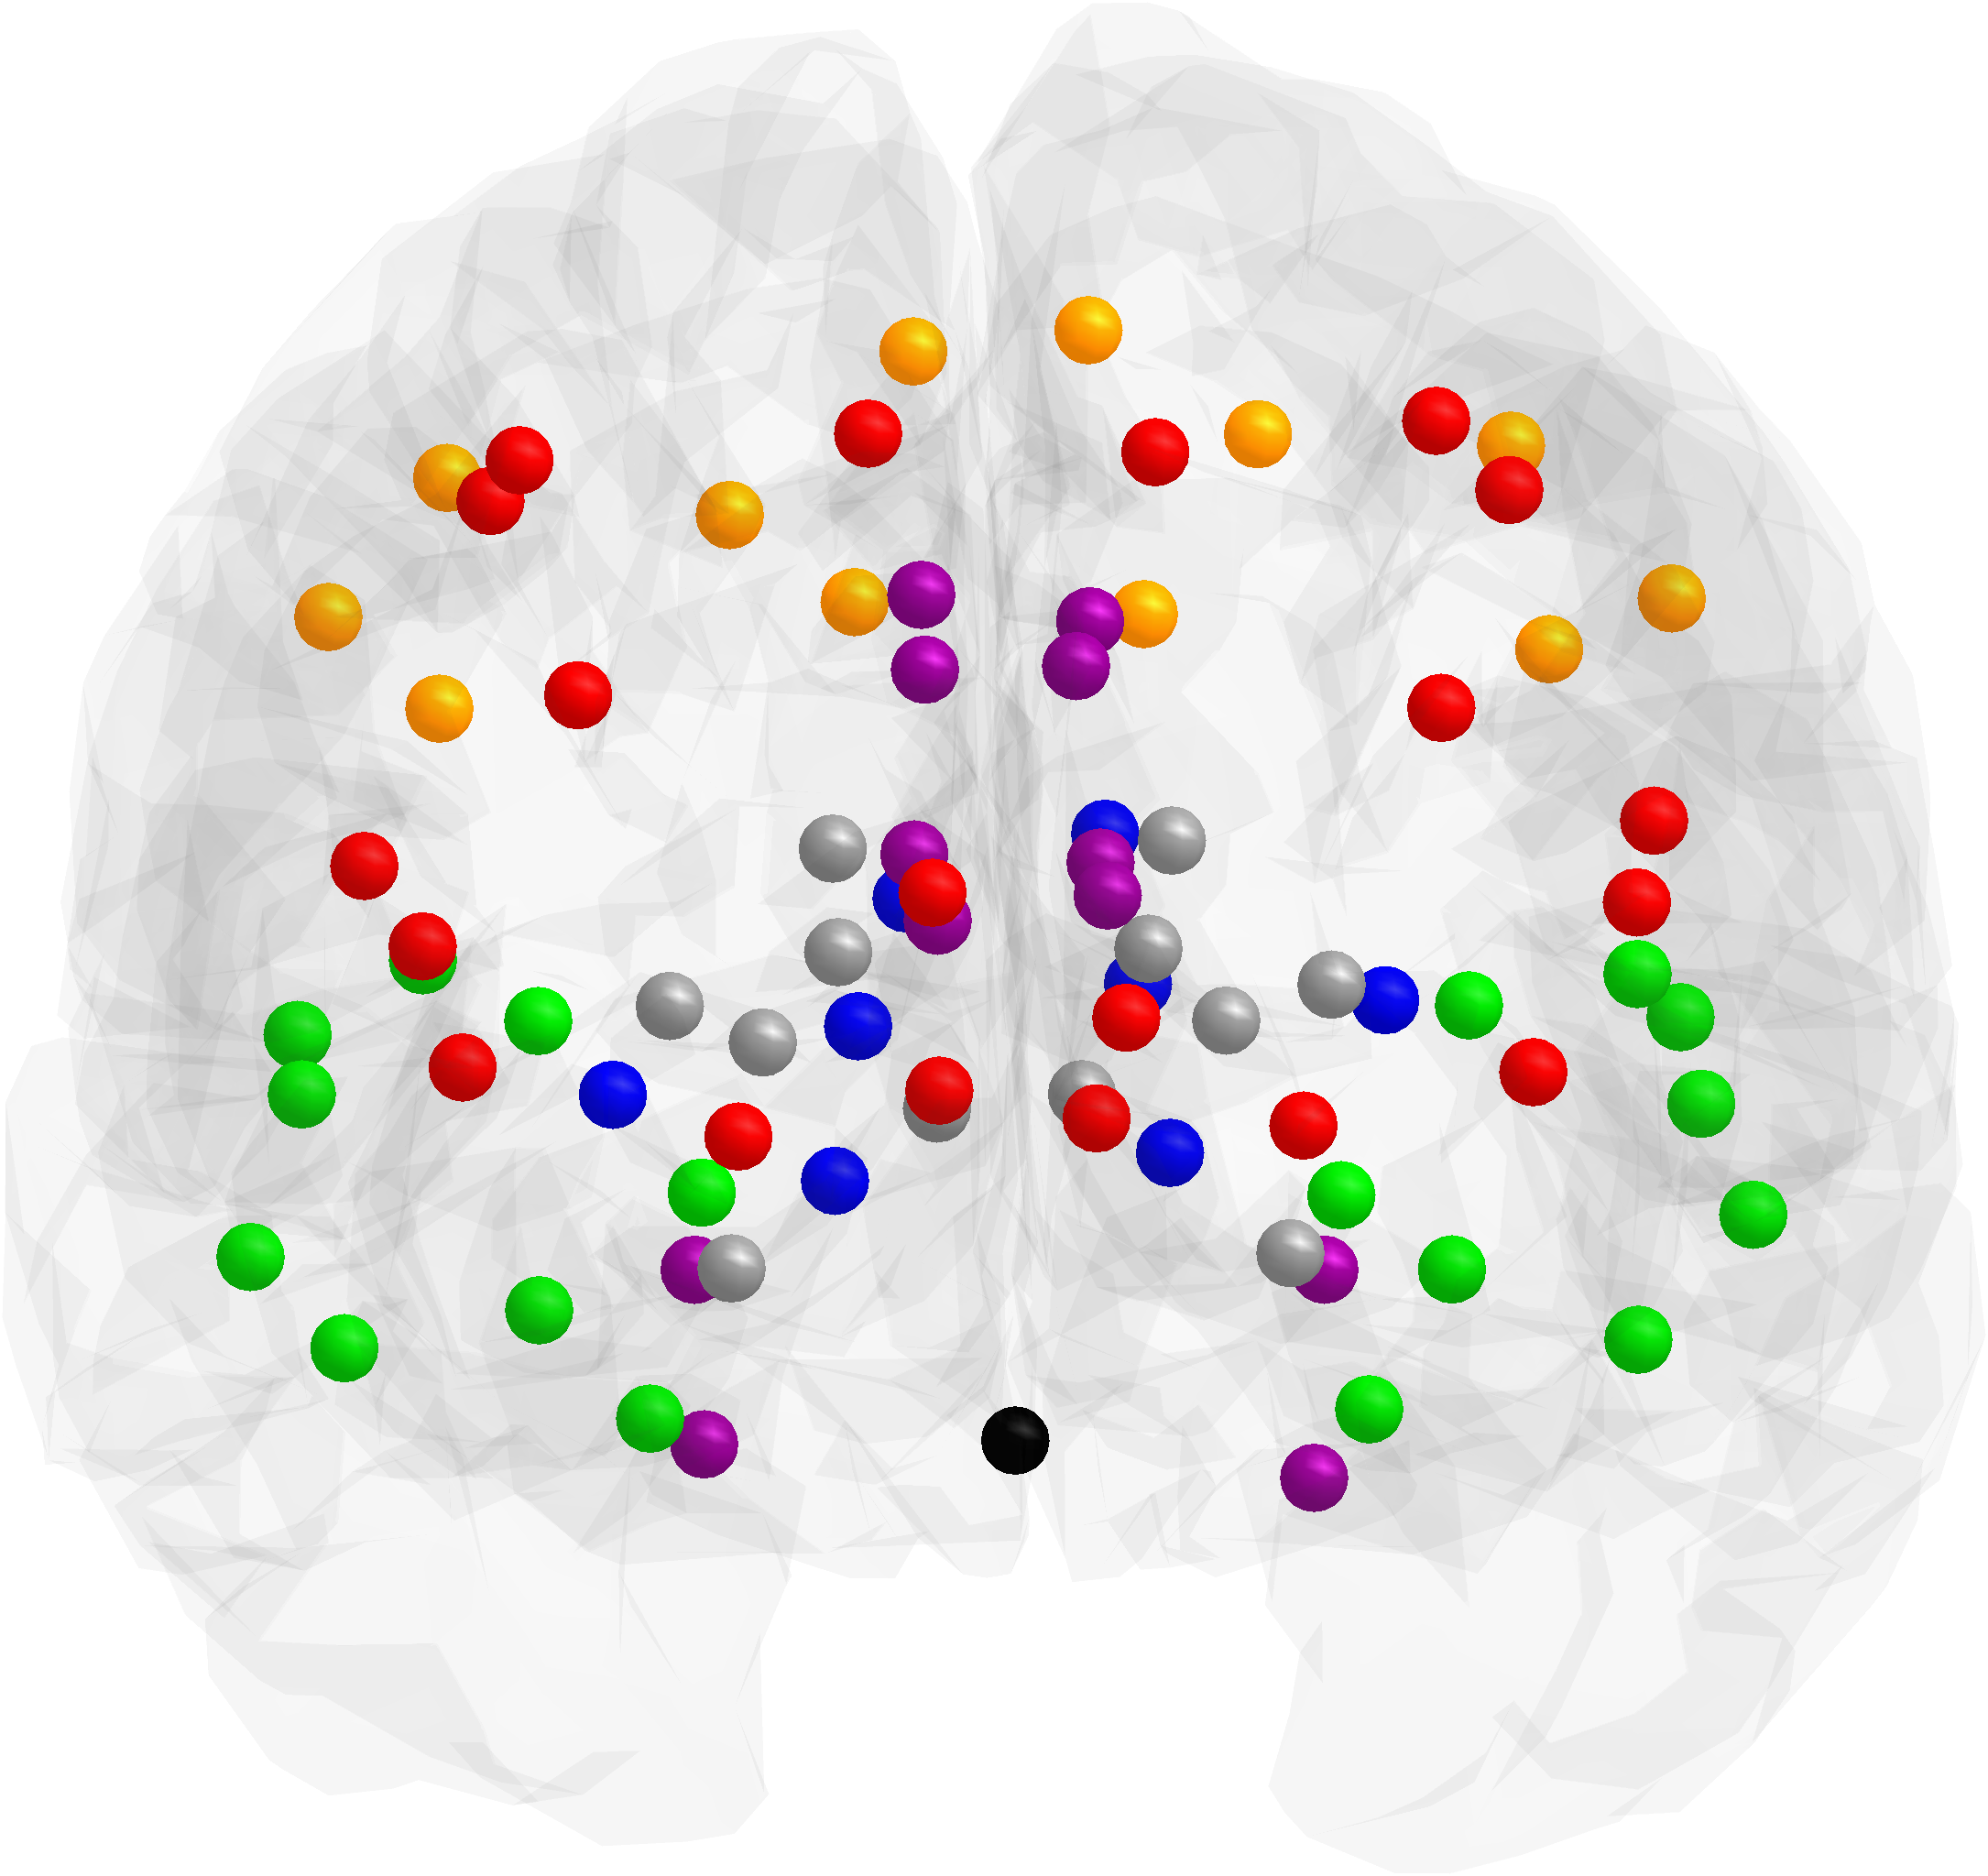
\includegraphics[height=\widthIm]
        {../Figure/regioniCervelloFronte [Trasparente].png}};
        % {../Figure/regioniCervelloFronte [Trasparente].png}};
    \node[anchor=north west] at (FKTimeScale c2r1.north west)
        {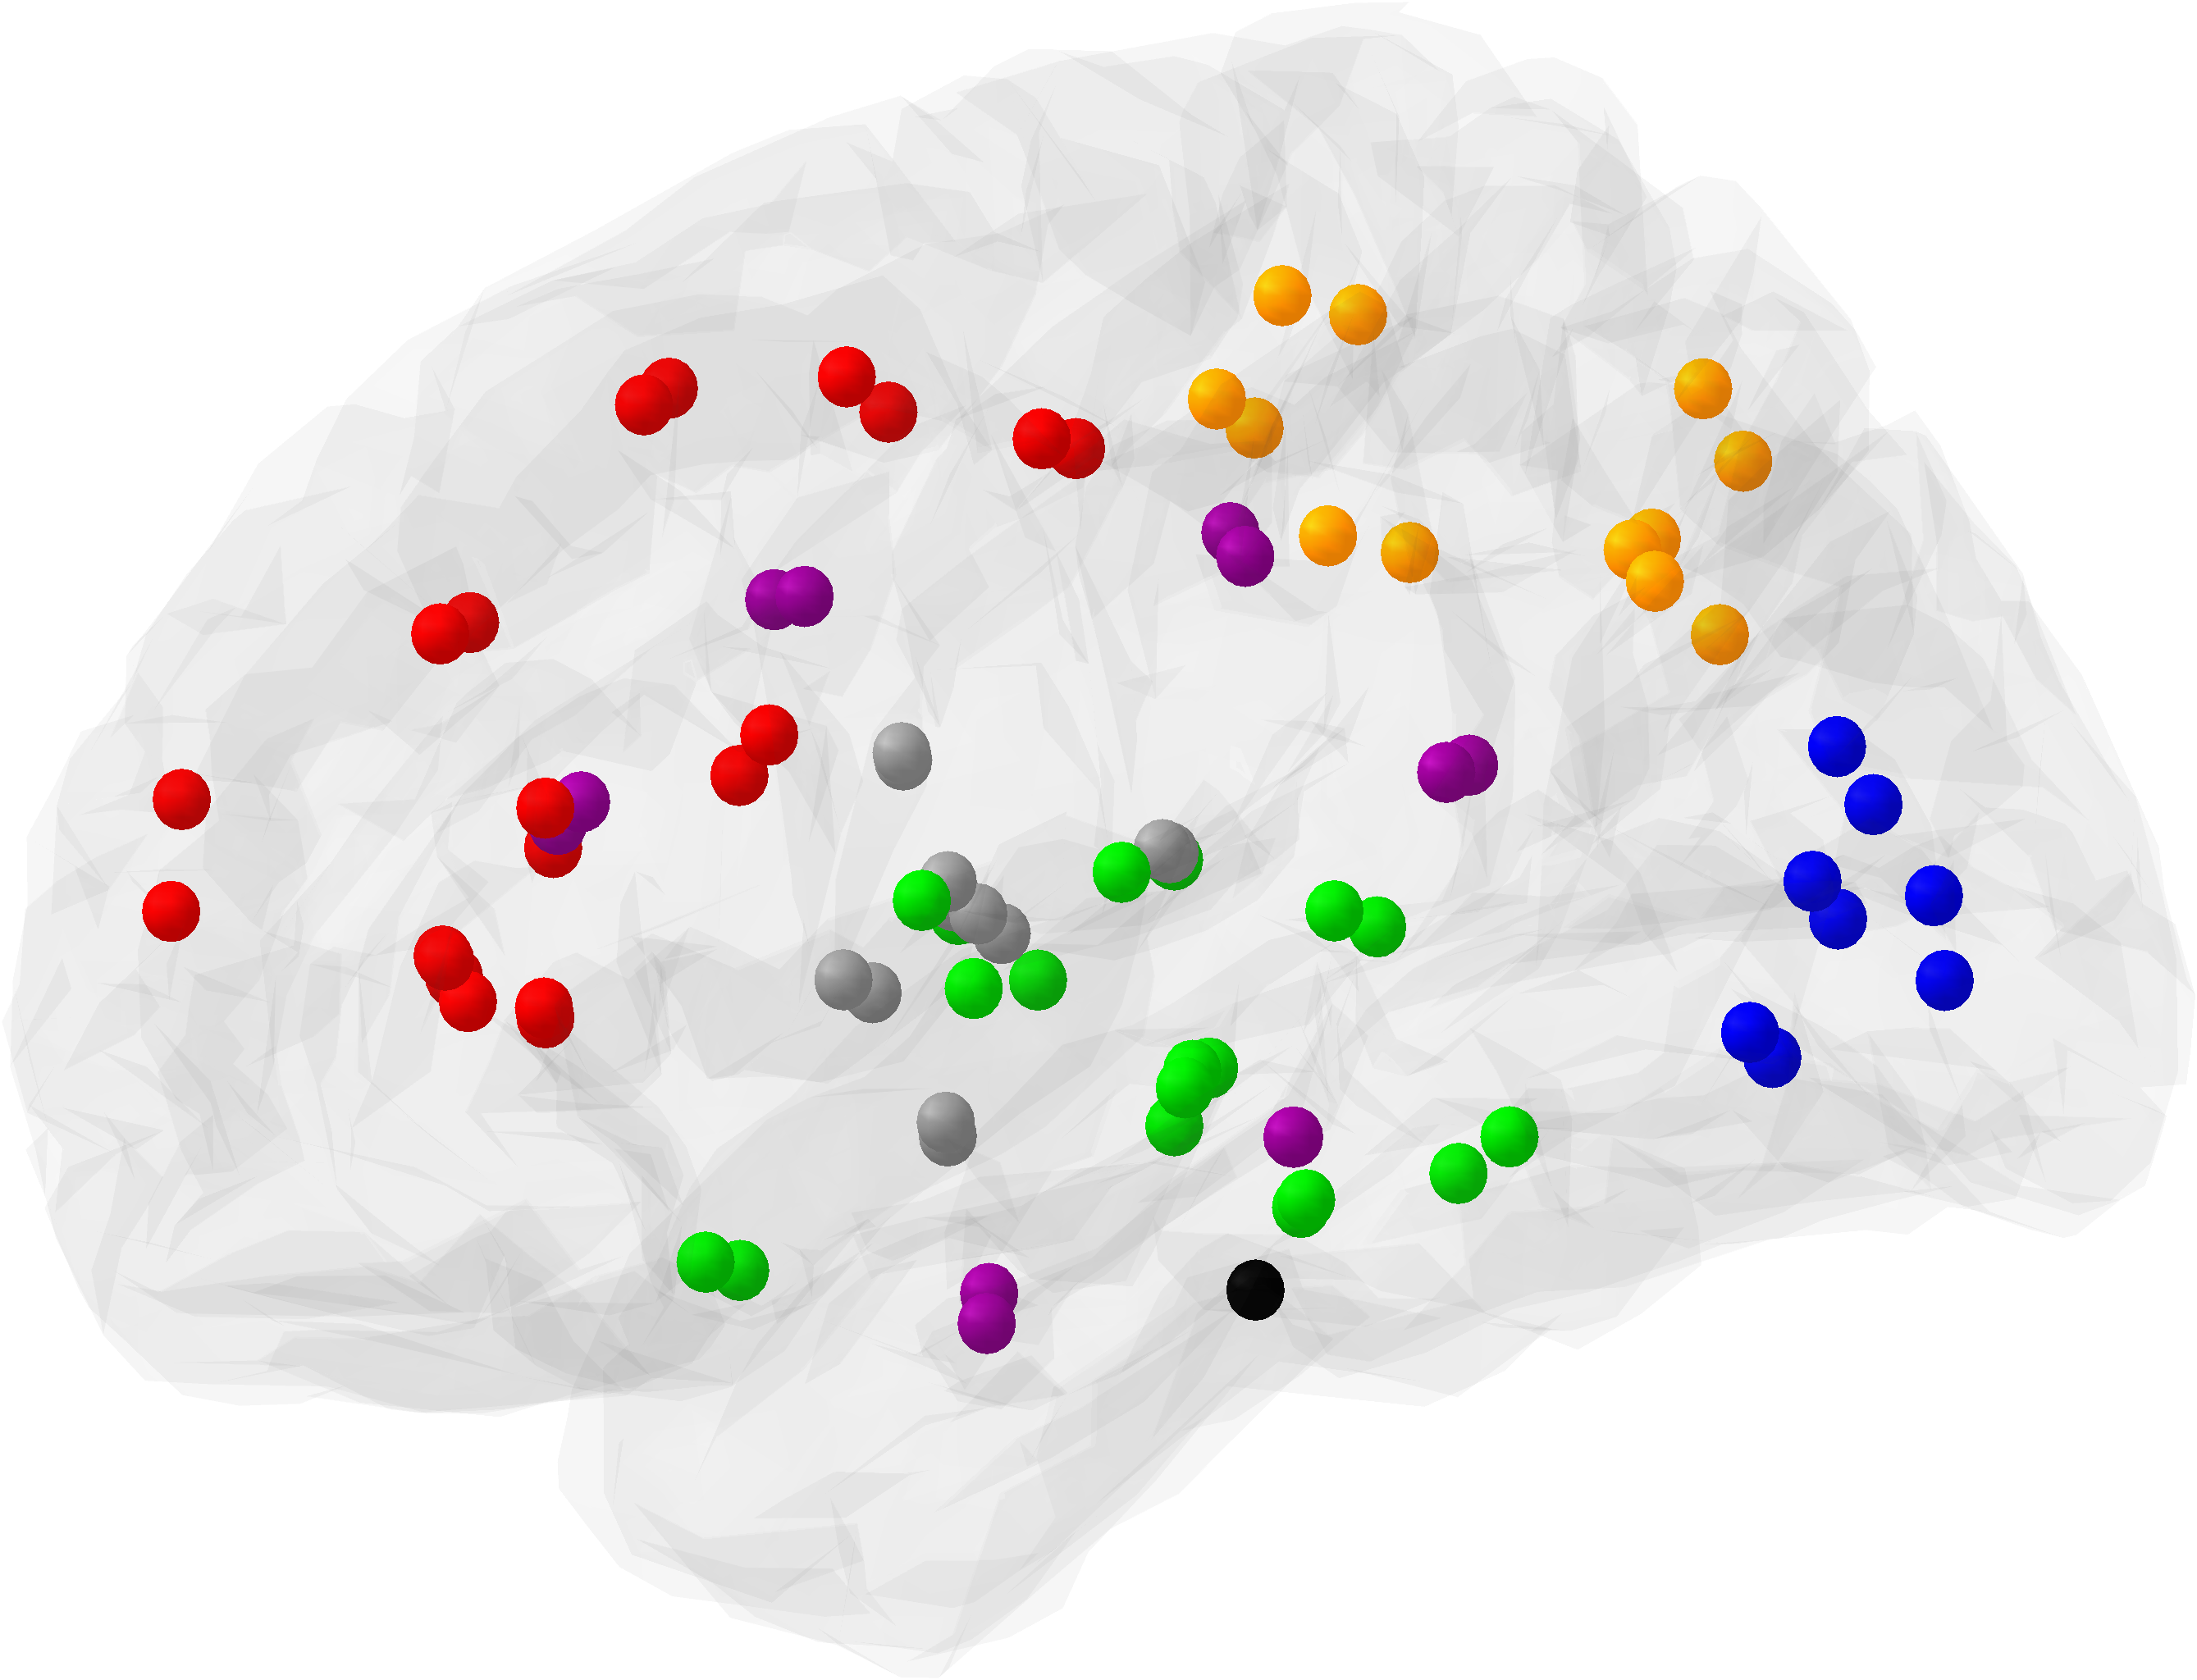
\includegraphics[height=\widthIm]
        {../Figure/regioniCervelloLato [Trasparente].png}};
        % {../Figure/regioniCervelloLato [Trasparente].png}};
    \node[anchor=north west] at (FKTimeScale c3r1.north west)
        {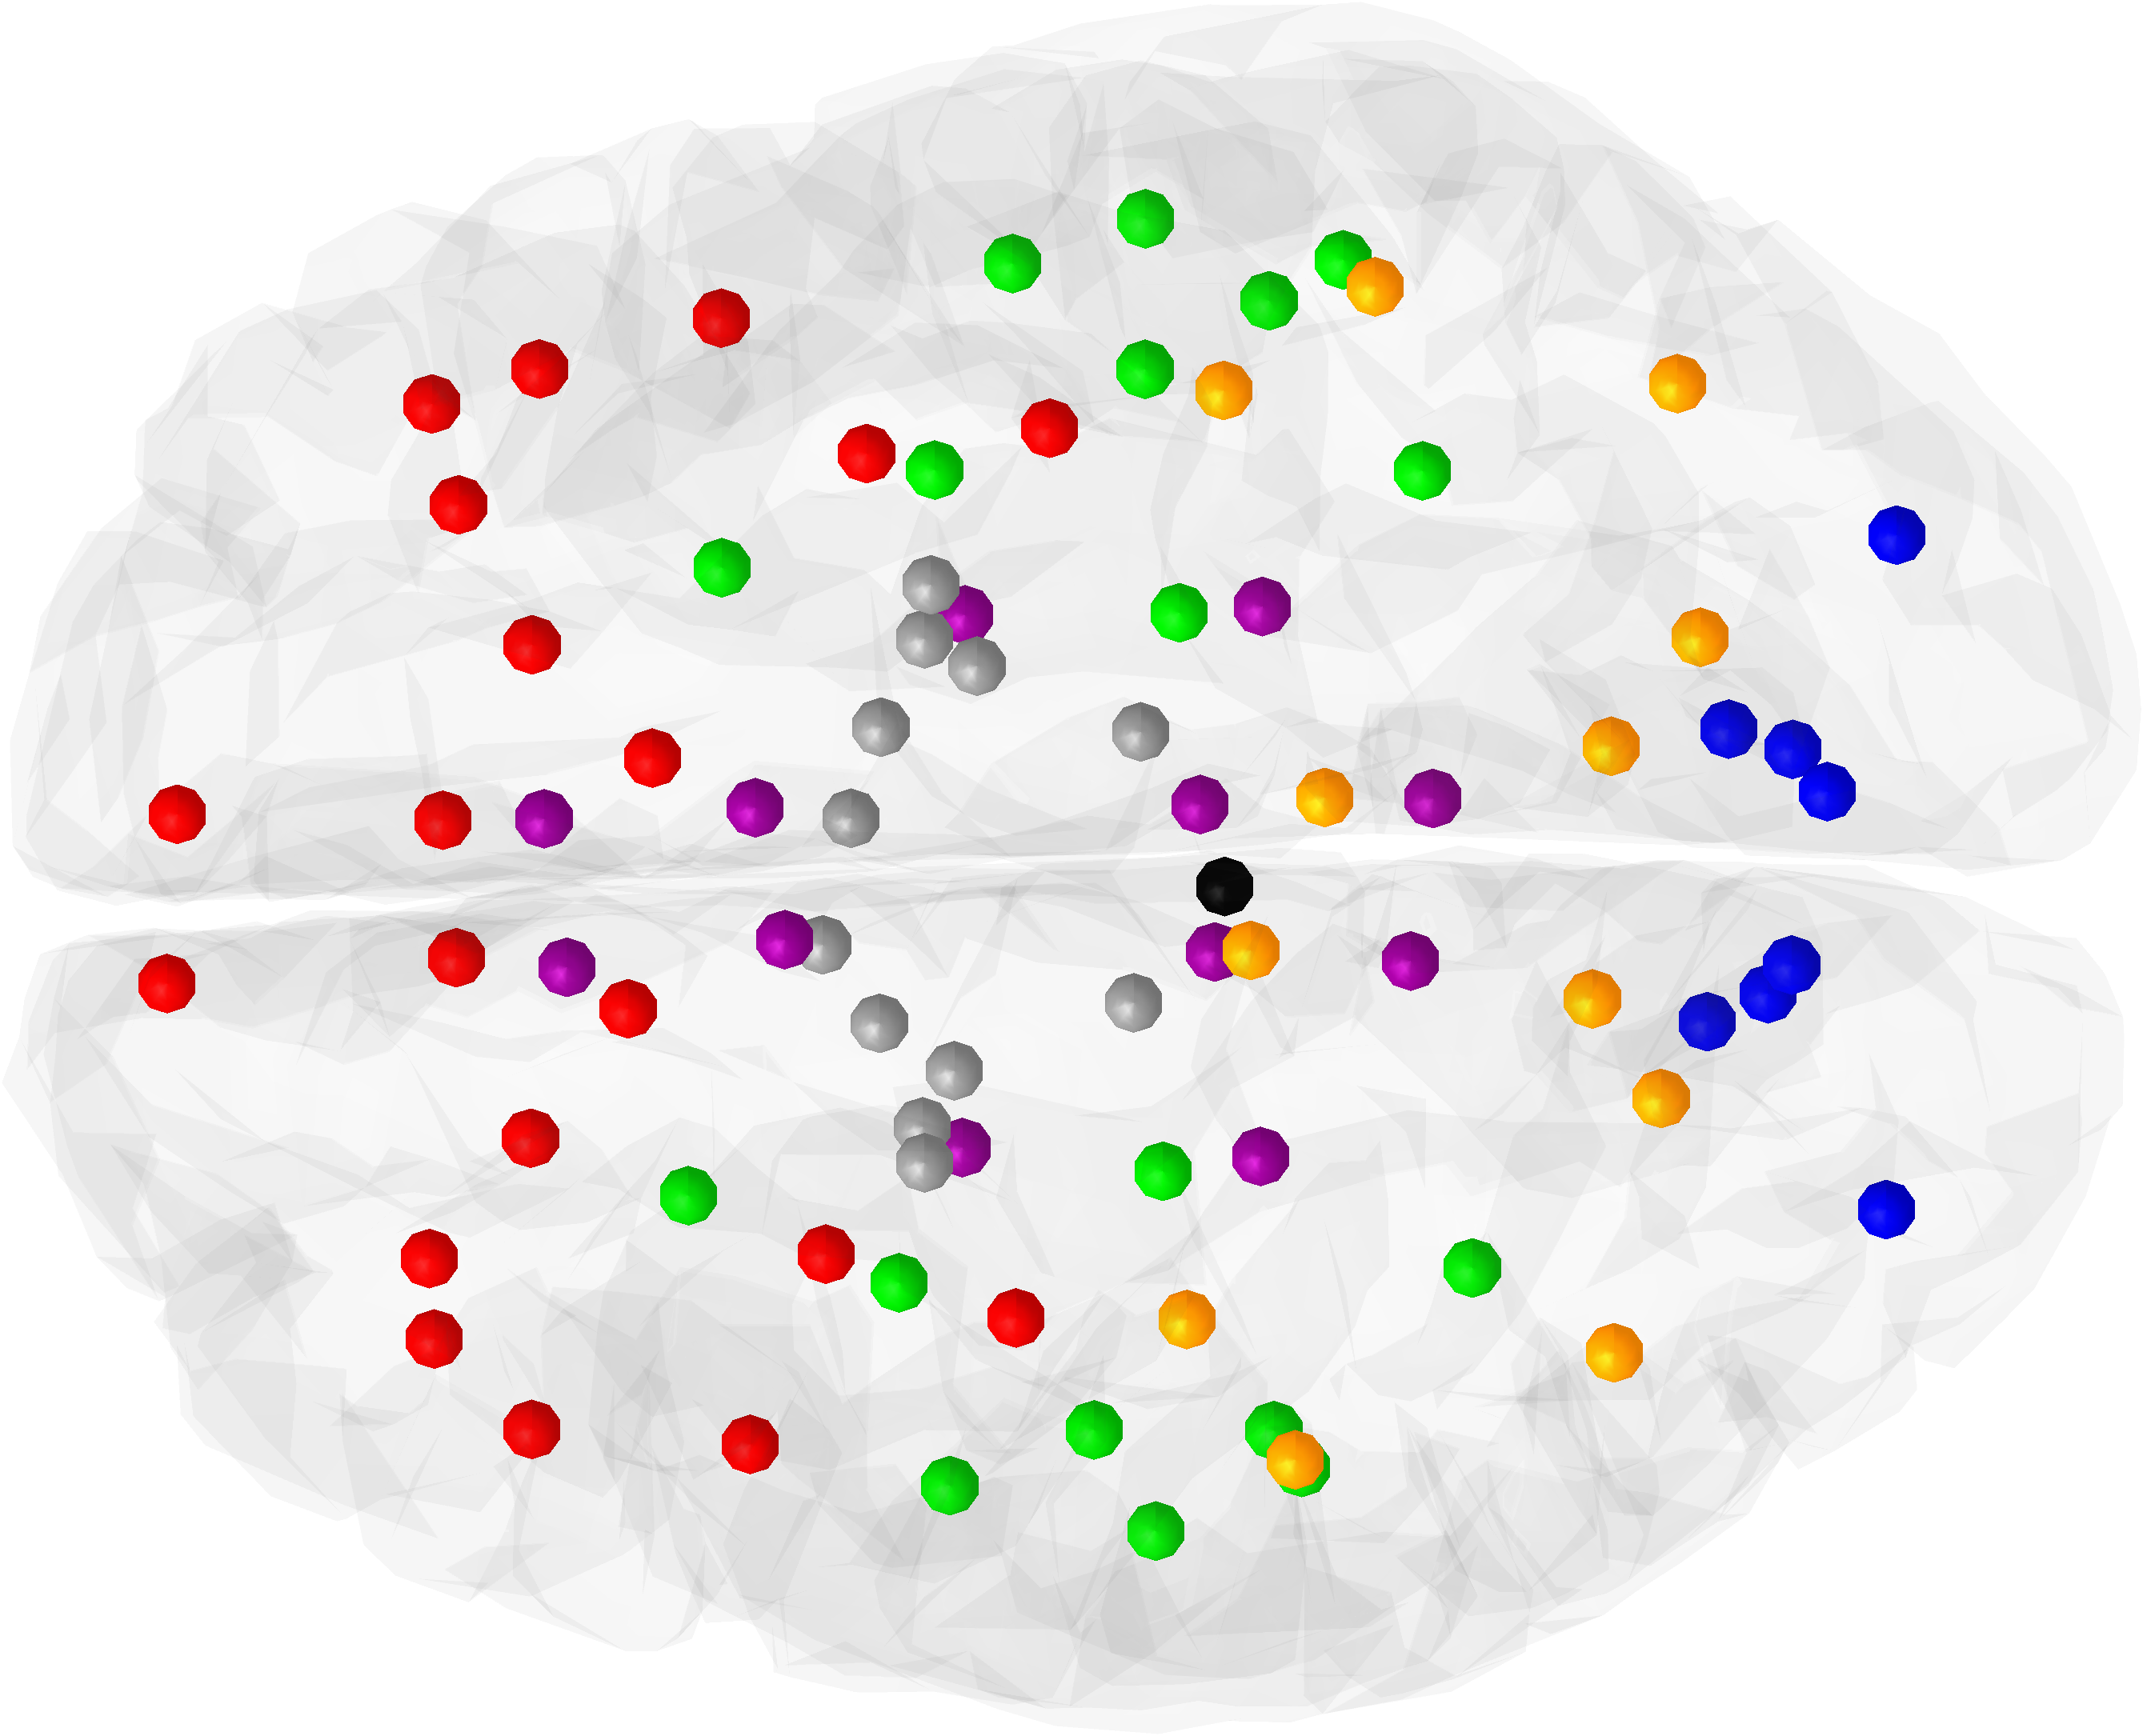
\includegraphics[height=\widthIm]
        {../Figure/regioniCervelloAlto [Trasparente].png}};
        % {../Figure/regioniCervelloAlto [Trasparente].png}};

    %

    \tikzset{SubCaption/.style={text width=4cm,anchor=south east,align=right}}
    \node[SubCaption] at (FKTimeScale c1r1.south east)
        {\dimTesto{\captionSize}\sottoDidascalia{$\tau_d\ll\tau_g$\label{figTimeScaledllg}}};
    \node[SubCaption] at (FKTimeScale c2r1.south east)
        {\dimTesto{\captionSize}\sottoDidascalia{$\tau_d\approx\tau_g$\label{figTimeScaledppg}}};
    \node[SubCaption] at (FKTimeScale c3r1.south east)
        {\dimTesto{\captionSize}\sottoDidascalia{$\tau_d\gg\tau_g$\label{figTimeScaledggg}}};
\end{tikzpicture}
}
                    {Three timescale cases in \FKdiscrete{} (see Tab. \ref{tabTimeScales} for $\rho$, timescale and $T_c$ data values). The plots have been generated using § \ref{secSettingsFK} setting, aside $\Delta t$ and $T$ which are set appropriately in each case, and the same logic found in § \ref{secResultsFKHD} (\ie{} with \eqref{eqFKHDConcentrationCurveFormula}).}
                    {.925\linewidth}
                    {figTimeScales}

                This is the reason why the Laplacian has to be multiplied by $\rho$ in \eqref{eqLaplacianMatrix}: it's necessary in order to have $\tau_d\approx\tau_g$, where $\tau_g$ can have any of the form considered in \cref{eqTauGFK,eqTauGHD,eqTauGSMO}, and thus a biologically sound dynamic.

                A possible choice or $\rho$ could be one such that $\tau_d=\tau_g$, that is
                %
                \begin{equation}
                    \tau_d=\frac1{\Vert\mathbf L\Vert_2}=
                    \frac1{\rho\Vert\boldsymbol{\mathcal L}\Vert_2}=\tau_g
                    \implies
                    \rho=\frac1{\tau_g\Vert\boldsymbol{\mathcal L}\Vert_2}.
                    \label{eqRhoDefinition}
                \end{equation}
                %
                More generally, the cases illustrated before, along with Fig. \ref{figTimeScales} and Tab. \ref{tabTimeScales}, actually imply the presence of a continuum: while $\tau_d\ll\tau_g$ manifests very rapidly with only a difference of two orders of magnitude (OOMs), $\tau_d\gg\tau_g$ is an extreme case needing a difference of eight OOMs; on the contrary $\tau_d\approx\tau_g$ manifests even when there is a difference of one OOM if $\tau_d>\tau_g$, whereas if $\tau_d<\tau_g$, even with the same OOM, the evolution starts to rapidly degenerate.

                Therefore, the true condition for a biologically sound dynamic is $\tau_d\gtrapprox\tau_g$ or, equivalently, for the OOMs\footnotemark{}
                %
                \begin{equation*}
                    \lfloor\log_{10}(\tau_d)\rfloor\ge
                    \lfloor\log_{10}(\tau_g)\rfloor,
                \end{equation*}
                % https://en.wiktionary.org/wiki/order_of_magnitude
                so \eqref{eqRhoDefinition} is only a \textit{sufficient} but not \textit{necessary} value for $\rho$.

                \footnotetext{
                    In scientific notation $a\in\RPlus$ is expressed as $a=b10^c$ with significand $b\in[1,10)$ and exponent $c\in\mathbb N$, \ie{} the order of magnitude; by then applying the logarithm base $10$ and floor function one has, since $\log_{10}(b)\in[0,1)$,
                    %
                    {\setlength\belowdisplayskip{0pt}%
                    \setlength\belowdisplayshortskip{0pt}%
                    \[
                        % \boxed{
                        \lfloor\log_{10}(a)\rfloor=
                        \lfloor\log_{10}(b)+c\rfloor=
                        \lfloor\log_{10}(b)\rfloor+\lfloor c\rfloor
                        =c.%}
                    \]}%
                    %
                    % \begin{equation*}
                    %     \lfloor\log_{10}(\tau_d)\rfloor=
                    %     \lfloor\log_{10}(\tau_g)\rfloor,
                    % \end{equation*}
                    %
                }

                \begin{table}[h]
                    \sisetup{scientific-notation=false}
                    %
                    \newcommand\yearNote{For «\unit{\year}» see § \ref{secSettings}.}
                    \newcommand\convergenceTimeNote{For «$T_c$» see § \ref{secAsymptoticAnalysisNetwork}.}
                    %
                    \newcommand\halfHeight{.1cm}
                    \newcommand\wCol{1cm}
                    \newcommand\hRow{\halfHeight}
                    \setlength\extrarowheight{\halfHeight}
                    \newcommand\sepCol{\hspace{1cm}}
                    %
                    \centering
                    \begin{NiceTabular}{
                        wc{\wCol}|
                        S[
                            table-format=1e2,
                            exponent-mode=scientific,
                            retain-zero-exponent=true,
                            % table-column-width=\wCol,
                        ]
                        S[
                            table-format={$\approx$}1e1,
                            exponent-mode=scientific,
                            % table-column-width=\wCol]
                        ]
                        S[
                            table-format=1e1,
                            exponent-mode=scientific,
                            retain-zero-exponent=true,
                            % table-column-width=\wCol]
                        ]
                        S[
                            table-format=2.2,
                            scientific-notation=false,
                        ]
                    }[
                        % corners,
                        %hvlines-except-borders,
                        % hvlines,
                        rounded-corners,
                        notes/para=true,
                        notes/style=\textit{\arabic{#1}},
                    ]
                    \CodeBefore
                        % \chessboardcolors{red!15}{blue!15}
                        % \chessboardcolors{black!15!white}{}
                        \rowcolors{1}{black!5!white}{black!15!white}
                    \Body
                        &{$\rho$}&{$\tau_d$ [\unit{\year}]\tabularnote{\yearNote}}
                        &{$\tau_g$ [\unit{\year}]\tabularnote{\yearNote}}
                        &{$T_c$ [\unit{\year}]\tabularnote{\yearNote}%
                        \tabularnote{\convergenceTimeNote}}\\[\hRow]\hline
                        $\tau_d\ll\tau_g$    &1e0  &{$\approx$}2e-2&2e0&20.04\\[\hRow]
                        $\tau_d\approx\tau_g$&1e-3 &{$\approx$}2e1 &2e0&29.69\\[\hRow]
                        $\tau_d\gg\tau_g$    &1e-10&{$\approx$}2e8 &2e0&92.35\\[\hRow]
                    \end{NiceTabular}
                    \caption{$\rho$, timescale and $T_c$ data of Fig. \ref{figTimeScales}.}
                    \label{tabTimeScales}
                \end{table}

            \subsubsection{Temporal discretization}\label{secTemporalDiscretization}

                The time discretization considered is the Euler method both implicit and explicit. To define it, first observe that all ODE systems in \FKdiscrete{}, \HDdiscrete{} and \SMOdiscrete{} can be represented as
                %
                \begin{equation}
                    \derT{\mathbf c}t=\mathbf F(\mathbf c(t),t;\mathbf L,\mathcal P),
                    \label{eqGenericSystemODE}
                \end{equation}
                %
                for a fixed Laplacian $\mathbf L$ and a set of parameters $\mathcal P$; of course, due to the quadratic terms, $\mathbf F$ is nonlinear.

                Given a uniform time step size $\Delta t\in\RPlusStar$ such that \[T/\Delta t=N\in\NPlus,\]then $\mathcal T$ is discretized by times steps \[t_n=n\Delta t\text{, with }1\le n\le N.\]

                The logic behind the Euler methods is to approximate the time derivative with a finite difference between two consecutive time steps:
                %
                \begin{equation*}
                    \derT{\mathbf c}t(t_{n+1})\approx
                    \frac{\mathbf c(t_{n+1})-\mathbf c(t_n)}{\Delta t},
                    \quad\forall n\in\{1,\ldots,N-1\}.
                \end{equation*}
                %
                By evaluating $\mathbf F(\mathbf c(t),t;\mathbf L,\mathcal P)$ in $t_n$ the explicit Euler method is obtained, with update rule
                %
                \begin{equation}
                    \mathbf c(t_{n+1})=\mathbf c(t_n)
                    +\Delta t\mathbf F(\mathbf c(t_n),t_n;\mathbf L,\mathcal P),
                    \label{eqUpdateRuleEE}
                \end{equation}
                %
                while in $t_{n+1}$ one has the implicit Euler method, with update rule
                %
                \begin{equation}
                    \mathbf c(t_{n+1})=\mathbf c(t_n)
                    +\Delta t\mathbf F(\mathbf c(t_{n+1}),t_{n+1};\mathbf L,\mathcal P).
                    \label{eqUpdateRuleEI}
                \end{equation}
                %
                Both are first-order methods but only the second one is unconditionally stable (A-stable), which in practice means any choice of $\Delta t>0$ results in a non-exploding solution in time whereas explicit methods need a sufficiently small time step for a non-exploding solution.

                Conversely, explicit methods are less computationally demanding compared to implicit ones as the latter, due to the nonlinearity of $\mathbf F$, have to solve a root-finding problem for the next value. \cite{MACNMonegato2008,NMFEDormand2018}

                Lastly, this procedure fully discretizes the solution that from \eqref{eqSpatialDiscretizedSol} becomes
                %
                \begin{equation}
                    \tilde c(\mathbf x,t_n)=
                    \sum_{i=k}^Vc^k(t_n)\mathbb1_{\text{ROI}_k}(\mathbf x)\approx
                    c(\mathbf x,t_n),
                    \label{eqTimeDiscretizedSol}
                \end{equation}
                %
                with $1\le n\le N$, which now lies in $\tilde c\in L_+^\infty(\STCyl)$.

        \subsection{Asymptotic analyses}\label{secAsymptoticAnalyses}

            To normalize the plots it's necessary to find a reference value and a natural choice is the asymptotic value of the misfolded $\tau$ proteins concentration.

            Each model is studied by searching its stable equilibrium points (EPs), \ie{} such that $\derTiL{}t=0$, when the system is homogeneous, namely $\DeltaD=0$ or $\mathbf L=\boldsymbol0$.

            Afterwards, an empiric formula is proposed to estimate the convergence time to reach it.

            \subsubsection{FK model}\label{secAsymptoticAnalysisFK}

                For \FKcontinuous{} one has
                %
                \begin{equation}
                    0=\alpha c_\infty\left(1-c_\infty\right)=f(c_\infty)
                    \label{eqFKContinuousAsymptoticEquation}
                \end{equation}
                %
                whose EPs are $c_\infty\in\{0,1\}$ as $c$ is, in fact, already dimensionless; however from the derivative
                %
                \begin{equation*}
                    f'(c_\infty)=\alpha-2\alpha c_\infty
                \end{equation*}
                %
                it holds
                %
                \begin{equation}
                    \left\{
                    \begin{alignedat}{2}
                        f'(0)&=\alpha>0&\;\;\implies\;\;&\text{unstable EP},\\
                        f'(1)&=-\alpha<0&\;\;\implies\;\;&\text{LAS EP},
                    \end{alignedat}
                    \right.
                    \label{eqFKEPStability}
                \end{equation}
                %
                where LAS stands for \textit{locally asymptotically stable} with basin of attraction $\mathcal A=\RPlusStar$ (see \cite{NLDCStrogatz2024} for more details): $1$ is the asymptotic value of all \FKcontinuous{} with IC $c_0\neq0$, with $\alpha$ only changing the time required to reach it.

                For \FKdiscrete{} one has
                %
                \begin{equation}
                    \boldsymbol0=\alpha\mathbf c\HadProd(1-\mathbf c),
                    \label{eqFKDiscreteAsymptoticEquation}
                \end{equation}
                %
                where each equation is like \eqref{eqFKContinuousAsymptoticEquation} but with $c^i_\infty$, $1\le i\le V$, in place of $c_\infty$; hence, the asymptotic network value is $Vc_\infty$.
                % moreover, since the system is homogeneous, it holds $\mathbf c_0=c_0\mathbf q=c_0\mathbf I$ with $c_0\neq0$, so every node tends towards $1$ and the asymptotic toxic vector is $\mathbf c_\infty=\mathbf I$.


            \subsubsection{HD model}\label{secAsymptoticAnalysisHD}

                For \HDcontinuous{} one has
                %
                \begin{equation}
                    \left\{
                    \begin{aligned}
                        0&=\gamma-\mu_hc^\infty_h-\kappa c^\infty_hc^\infty_m,\\[5pt]
                        0&=-\mu_mc^\infty_m+\kappa c^\infty_hc^\infty_m,
                    \end{aligned}
                    \right.
                    \label{eqHDContinuousAsymptoticSystem}
                \end{equation}
                %
                for which there are two EPs:
                %
                \begin{equation}
                    \newcommand\vspcR{2pt}
                    \mathbf c_1\left\{
                    \begin{aligned}
                        c_{h,1}^\infty&=\frac\gamma{\mu_h},\\[\vspcR]
                        c_{m,1}^\infty&=0,
                    \end{aligned}
                    \right.
                    \quad\text{and}\quad
                    \mathbf c_2\left\{
                    \begin{aligned}
                        c_{h,2}^\infty&=\frac{\mu_m}\kappa,\\[\vspcR]
                        c_{m,2}^\infty&=\frac{\left(\kappa\gamma-\mu_h\mu_m\right)}{\mu_m\kappa}.
                    \end{aligned}
                    \right.
                    \label{eqHDEP}
                \end{equation}
                %
                From \eqref{eqHDEP} it's clear $\mathbf c_2$ exists iff $k\gamma>\mu_h\mu_m$, otherwise it's either equal to $\mathbf c_1$ ($k\gamma=\mu_h\mu_m$) or $c_{m,2}^\infty$ becomes negative ($k\gamma<\mu_h\mu_m$) and thus biologically illogical.

                Hence, assuming $k\gamma>\mu_h\mu_m$, it's possible, by studying the Jacobian of \eqref{eqHDContinuousAsymptoticSystem}, to show (see Appendix \ref{apxAsymptoticHDCalcs}) that $\mathbf c_2$ in the $(c_h,c_m)$ plane is LAS, with
                %
                \begin{equation*}
                    \mathcal A_2=\RPlus\times\RPlusStar,
                \end{equation*}
                %
                whereas $\mathbf c_1$ is unstable, though it attracts the $x$-axis, \ie{}
                %
                \begin{equation*}
                    \mathcal A_1=\RPlus\times\{0\}.
                \end{equation*}
                %
                For \HDdiscrete{} one has
                %
                \begin{equation}
                    \left\{
                    \begin{aligned}
                        0&=\gamma\bOne
                        -\mu_h\mathbf c_h-\kappa\mathbf c_h\HadProd\mathbf c_m,\\[5pt]
                        0&=-\mu_m\mathbf c_m+\kappa\mathbf c_h\HadProd\mathbf c_m,
                    \end{aligned}
                    \right.
                    \label{eqHDDiscreteAsymptoticSystem}
                \end{equation}
                %
                where for each node is described by a system like \eqref{eqHDContinuousAsymptoticSystem} but with $c^{i,\infty}_h$ and $c^{i,\infty}_m$, $1\le i\le V$, in place of $c^\infty_h$ and $c^\infty_m$; thus, the asymptotic network values is $V$ times $\mathbf c_1$ or $\mathbf c_2$.
                % In addition, since the system is homogeneous, it holds $\mathbf c_{m,0}=c_{m,0}\mathbf q=c_{m,0}\mathbf I$ with $c_{m,0}\neq0$, so every vertex tends towards $\mathbf c_2$ and the asymptotic toxic vector is $\mathbf c_m^\infty=c_{m,2}^\infty\mathbf I$.


            \subsubsection{SMO model}\label{secAsymptoticAnalysisSMO}

                For this case it's very difficult to gain asymptotic information on the concentrations by studying the single equations as they are far too complex to handle.

                However, an equivalent analysis is possible regarding the moments of the toxic aggregates
                %
                \begin{equation}
                    Q_i=\sum_{l=2}^{\infty}l^ic_l,
                    % \implies
                    % \left\{\begin{aligned}
                    %     P\equiv Q_0&\quad\text{total toxic number},\\
                    %     M\equiv Q_1&\quad\text{total toxic mass},
                    % \end{aligned}\right.
                    \label{eqMomentDefinition}
                \end{equation}
                %
                where only the first two are of interests:
                \begin{itemize}[%
                    topsep=7.5pt,	  % Spazio superiore tra testo e lista
                    itemsep=-2pt,	  % Spazio tra gli elementi («item») della lista
                    leftmargin=20pt,  % Spazio tra la lista e il bordo destro del testo
                    rightmargin=0pt,  % Spazio tra la lista e il bordo sinistro del testo
                    %itemindent=!,
                    % labelindent=30pt, % Spazio tra il margine sinistro e l'etichetta della lista
                    %labelwidth=!,
                    %labelsep=!
                    % \leftmargin + \itemindent = \labelindent + \labelwidth + \labelsep
                ]
                    \item the total number of toxic aggregates $P\equiv Q_0$ and
                    \item the total toxic mass $M\equiv Q_1$, expressible also as
                    %
                    \begin{equation}
                        M=\sum_{i=1}^\infty ic_i-c_1\equiv\TotM-m
                        \implies\TotM=m+M
                        \label{eqDecompositionTotalMass}
                    \end{equation}
                    %
                    with $m$ being the healthy monomer concentration while $\TotM$ the total mass.
                \end{itemize}

                To gather the necessary equations the following assumption is made: the number of $\tau$ polymers $L$ is sufficiently large as to not affect the dynamics on intermediate time scales of disease progression. \cite[§ 5.2]{Goriely2019} In essence it means that the sum over all equations in \SMOcontinuous{} is well approximated by the sum in the $L\to\infty$ limit.

                Consequently, a new system of three equations can be derived by considering the first one in \SMOcontinuous{}, with $m\equiv c_1$, the second as the sum over all equations with $i\ge2$ in \SMOcontinuous{} and likewise the third but with the $i$-th equation multiplied by $i$ (see Appendix \ref{apxSystemOfMoments}):
                %
                \begin{subequations}
                    \label{eqContinuousMomentEquations}
                    \newcommand\vspcR{2pt}
                    \begin{empheq}[left=\empheqlbrace]{align}
                        \derT mt&=\DeltaD m+\gamma-\mu m-2\boldsymbol\kappa m^2-amP,
                        \label{eqmContinuousMomentEquation}\\[\vspcR]
                        \derT Pt&=\DeltaD P-\mu P+\kappa m^2+\frac f2(M-3P+c_2),
                        \label{eqPContinuousMomentEquation}\\[\vspcR]
                        \derT Mt&=\DeltaD M-\mu M+2\boldsymbol\kappa m^2+amP.
                        \label{eqMContinuousMomentEquation}
                    \end{empheq}
                \end{subequations}%
                %
                Define now $\mInf, \PInf, \MInf\in\RPlus$ as the asymptotic values of the respective unknowns such that \eqref{eqContinuousMomentEquations} become
                %
                \begin{subequations}
                    \label{eqAsymptoticMomentEquations}
                    \newcommand\vspcR{2pt}
                    \begin{empheq}[left=\empheqlbrace]{align}
                        0&=\gamma-\mu\mInf-2\boldsymbol\kappa\mInf^2-a\mInf\PInf,
                        \label{eqmAsymptoticMomentEquation}\\[\vspcR]
                        0&=-\mu\PInf+\kappa\mInf^2+\frac f2(\MInf-3\PInf),
                        \label{eqPAsymptoticMomentEquation}\\[\vspcR]
                        0&=-\mu\MInf+2\boldsymbol\kappa\mInf^2+a\mInf\PInf,
                        \label{eqMAsymptoticMomentEquation}
                    \end{empheq}
                \end{subequations}%
                %
                where $fc_2$ has been neglected since both terms are expected to be small\footnotemark{}, at least initially.

                \footnotetext{This approximation is actually indistinguishable from the full system solution as can be seen in \cite[Fig. 8]{Goriely2019}.}

                However, the system \eqref{eqAsymptoticMomentEquations} is not yet autonomous as $\boldsymbol\kappa$ is not homogeneous in space due to its assumed definition in \eqref{eqNucleationIndicatorFunction}. The solution is to average \eqref{eqAsymptoticMomentEquations} in space: all the unknowns and parameters will remain unchanged whereas $\boldsymbol\kappa$ becomes
                %
                \begin{equation}
                    \begin{aligned}
                        \bar{\boldsymbol\kappa}&=
                        \frac1{\Vol{\Omega}}\int_\Omega\boldsymbol\kappa\de\mathbf x=
                        \frac\kappa{\Vol{\Omega}}\int_\Omega\mathbb1_{\mathcal K}\de\mathbf x\\
                        &=\frac\kappa{\Vol{\Omega}}\int_{\mathcal K}1\de\mathbf x=
                        \kappa\frac{\Vol{\mathcal K}}{\Vol{\Omega}}\equiv\kappa\varphi.
                    \end{aligned}
                    \label{eqContinuousAverageNucleation}
                \end{equation}
                %
                Using \eqref{eqContinuousAverageNucleation}, $\PInf$ is obtained by isolating it from \eqref{eqmAsymptoticMomentEquation}:
                %
                \begin{equation}
                    \PInf=\frac{\gamma-\mu\mInf-2\kappa\varphi\mInf^2}{a\mInf},
                    \label{eqPInfValue}
                \end{equation}
                %
                which used in \eqref{eqMAsymptoticMomentEquation} gives
                %
                \begin{equation}
                    \MInf=\frac\gamma\mu-\mInf\ \ \implies\ \
                    \TotM^\infty=\MInf+\mInf=\frac\gamma\mu.
                    \label{eqMInfValue}
                \end{equation}
                %
                This last result is also derived by finding the LAS EP of the equation obtained by summing \cref{eqmContinuousMomentEquation,eqMContinuousMomentEquation} and neglecting diffusion:
                %
                \begin{equation}
                    \derT\TotM t=\gamma-\mu\TotM,
                    \label{eqMassConservation}
                \end{equation}
                %
                where if $\TotM(0)=\gamma/\mu$ then the total mass is conserved; for this reason \eqref{eqMInfValue} is known as the mass conservation constrain as well.

                Thereafter, using \cref{eqPInfValue,eqMInfValue} in \eqref{eqPAsymptoticMomentEquation}, one finds a third order polynomial equation
                %
                \begin{equation}
                    q_3\mInf^3+q_2\mInf^2+q_1\mInf+q_0=0
                    % 2\boldsymbol\kappa\mInf^3
                    % +[4\mu\kappa+f(6\kappa-1)]\mInf^2
                    % +[2\mu^2+f(3\mu+1)]\mInf
                    % -\gamma(2\mu+3f)=0
                    \label{eqmInfEstimateEquation}
                \end{equation}
                %
                with
                %
                \begin{equation}
                    \SpazMate{1}{1}{1}
                    \newcommand\vspcR{2pt}
                    \newcommand\hspcC{\hspace{.3cm}}
                    \begin{alignedat}{2}
                        q_3&=2a\kappa\varphi,\hspcC%\\[\vspcR]
                        &q_2&=4\mu\kappa\varphi+f(6\kappa\varphi-a),\\[\vspcR]
                        q_1&=2\mu^2+f[3\mu+a(\gamma/\mu)],\hspcC%\\[\vspcR]
                        &q_0&=-\gamma(2\mu+3f).\\[\vspcR]
                    \end{alignedat}
                    \label{eqmInfCoefficientsEstimateEquation}
                \end{equation}
                %
                The roots of \eqref{eqmInfEstimateEquation} can be found with Cardano's formula \cite{AlgebraVanWaerden2003,HAKurosh1972}, although, due to the solution complexity, their symbolic form is of little use; indeed, one then needs to use them to find $\MInf$ and $\PInf$, with \cref{eqMInfValue,eqPInfValue} respectively, and finally to evaluate the Jacobian of \eqref{eqAsymptoticMomentEquations} to establish their nature as LAS or unstable. Therefore, the analysis of the EPs nature is omitted.
                % https://encyclopediaofmath.org/wiki/Cardano_formula

                Nevertheless, in the cases studied in § \ref{secSettings}, we can at least numerically say the solution satisfying the positivity constraints (see Appendix \ref{apxSMOPositivityAsmptoticConstraint}) is the smallest root of \eqref{eqmInfEstimateEquation}; this result seems to be confirmed [but not proven\footnotemark{}] by \cite{Goriely2019}.

                \footnotetext{Indeed, in \cite[§ 5.5 on p. 10]{Goriely2019} they only give upper and lower bounds for $\mInf$ without studying the EP nature.}

                For \SMOdiscrete{} one has to slightly change the moment definition which becomes vectorial
                %
                \begin{equation*}
                    \mathbf Q_i=\sum_{l=2}^{\infty}l^i\mathbf c_l,
                \end{equation*}
                %
                with $\mathbf P\equiv\mathbf Q_0$ and $\mathbf M\equiv\mathbf Q_1$. Then, applying to \SMOdiscrete{} the same reasoning resulting in \eqref{eqAsymptoticMomentEquations}, leads to
                %
                % \begin{subequations}
                %     \newcommand\vspcR{2pt}
                %     \begin{empheq}[left=\empheqlbrace]{align}
                %         \boldsymbol0&=\gamma\bOne
                %         -\mu\mInf\bOne-2\mInf^2\boldsymbol\kappa-\mInf\PInf\bOne,
                %         \label{eqmDiscreteMomentEquation}\\[\vspcR]
                %         \boldsymbol0&=-\mu\PInf\bOne+\mInf^2\boldsymbol\kappa
                %         +\frac f2(\MInf\bOne-3\PInf\bOne),
                %         \label{eqPDiscreteMomentEquation}\\[\vspcR]
                %         \boldsymbol0&=-\mu\MInf\bOne+2\mInf^2\boldsymbol\kappa+\mInf\PInf\bOne.
                %         \label{eqMDiscreteMomentEquation}
                %     \end{empheq}
                %     \label{eqDiscreteMomentEquations}
                % \end{subequations}
                %
                \begin{equation*}
                    \newcommand\vspcR{2pt}
                    \left\{
                    \begin{aligned}
                        \boldsymbol0&=\gamma\bOne-\mu\mInf\bOne
                        -2\mInf^2\boldsymbol\kappa-\mInf\PInf\bOne,\\[\vspcR]
                        \boldsymbol0&=-\mu\PInf\bOne+\mInf^2\boldsymbol\kappa
                        +\frac f2(\MInf\bOne-3\PInf\bOne),\\[\vspcR]
                        \boldsymbol0&=-\mu\MInf\bOne+2\mInf^2\boldsymbol\kappa+\mInf\PInf\bOne.
                    \end{aligned}
                    \right.
                \end{equation*}
                %
                Once again $\boldsymbol\kappa$ is non-null only in some nodes rendering the system non-autonomous and, like \eqref{eqContinuousAverageNucleation}, we can solve this issue by averaging over all nodes:
                %
                \begin{equation}
                    \begin{aligned}
                        \bar{\boldsymbol\kappa}&=
                        \frac1V\sum_{i=1}^V\kappa_i=
                        \kappa\frac qV\equiv\kappa\varphi.
                    \end{aligned}
                    \label{eqDiscreteAverageNucleation}
                \end{equation}
                %
                Thus the formulas for the discrete asymptotic values are the same as \cref{eqMInfValue,eqPInfValue,eqmInfEstimateEquation}, but with a different $\varphi$ definition and valid at each vertex, so that the asymptotic network values are $V$ times the previous ones.

                In conclusion, it's also possible to estimate the asymptotic size distribution \cite[(87, 88) on p. 12]{Goriely2019} (see Appendix \ref{apxAsymptoticSizeDistribution}):
                %
                \begin{equation}
                    c^\infty(n)=\PInf K(n)
                    \exp\left[\frac{4(f+\mu)^2-(2\mu+nf)^2}{4af\mInf}\right],
                    \label{eqAsymptoticSizeDistribution}
                \end{equation}
                %
                with
                %
                \begin{equation*}
                    K(n)=\frac{(2\mu+nf)^2-2af\mInf}{4a\mInf(f+\mu)},
                \end{equation*}
                %
                where the maximum concentration is reached by the polymer with size closest to
                %
                \begin{equation}
                    n_{\max}=\sqrt{6a\frac\mInf f}-2\frac\mu f.
                    \label{eqAsymptotic}
                \end{equation}

            \subsubsection{Convergence time}\label{secAsymptoticAnalysisNetwork}

                One might find reasonable to estimate the time necessary for the three models to reach their respective asymptotic values, based on their parameters $\mathcal P$.

                Unfortunately this is easier said than done, in part due to the nonlinear nature of the problem at hand; nonetheless, it's natural to assume that if one does exist it must depend on the time scales found in § \ref{secCharacteristicTimes}.

                We here propose one such function based empirically on the cases in § \ref{secSettings}:
                %
                \begin{equation}
                    T_c=10\tau_gf(\tau_d/\tau_g)=10\tau_g\left[\frac9{20}\log_{10}\left(\frac{\tau_d}{\tau_g}+1\right)+1\right],
                    \label{eqConvergenceTimeFunction}
                \end{equation}
                %
                from which the following remarks can be made:

                \begin{enumerate}[
                    label=R\arabic*, % Cambia l'etichetta degli elementi («item») (quella scritta si traduce in 1., 2. ecc.)
                    topsep=7.5pt,	  % Spazio superiore tra testo e lista
                    itemsep=-1pt,	  % Spazio tra gli elementi («item») della lista
                    leftmargin=30pt,  % Spazio tra la lista e il bordo destro del testo
                    rightmargin=20pt, % Spazio tra la lista e il bordo sinistro del testo
                    % \leftmargin + \itemindent = \labelindent + \labelwidth + \labelsep
                    %itemindent=!,
                    % labelindent=30pt,  % Spazio tra il margine sinistro e l'etichetta della lista
                    %labelwidth=!,
                    %labelsep=!
                ]
                    \item if $\tau_d\ll\tau_g$ then the network behaves like one no\-de (§ \ref{secCharacteristicTimes}) and $f(\tau_d)\approx1$;
                    \item\label{rmkDiffusionContributionConvergenceTime} if $\tau_d>\tau_g$ then diffusion is going to slow down convergence but only slightly as only a small quantity is needed to spark growth;
                    \item $9/20$ was chosen as to almost double $f(\tau_d/\tau_g)$ when $\log_{10}(\tau_d/\tau_g+1)$ doubles as well\footnotemark{};
                    \item $10$ comes from the observations that the convergence time of a single node is tenfold the initial estimated time;
                    \item as § \ref{secCharacteristicTimes}, \eqref{eqConvergenceTimeFunction} is \textit{not} a precise estimation of the convergence time, but it must be rather seen as an approximation of the OOM, \ie{} $\lfloor\log_{10}(T_c)\rfloor$, necessary to asymptotically converge.
                \end{enumerate}

                \footnotetext{For instance, if $\tau_d/\tau_g$ goes from $10^{10}$ to $10^{20}$, doub\-ling $\log_{10}(\tau_d/\tau_g+1)$, then  $f(\tau_d/\tau_g)$ almost doubles from $5.5$ to $10$.}

                Assumption \ref{rmkDiffusionContributionConvergenceTime} is motivated with the following reasoning: from § \cref{secAsymptoticAnalysisFK,secAsymptoticAnalysisHD,secAsymptoticAnalysisSMO} it's clear the only LAS EPs are those with a non-null toxic concentration; hence, if \[1\ll\tau_d/\tau_g<+\infty,\]$\mathbf L\mathbf c$ can be seen as the application of small perturbations to healthy nodes until their state changes from the unstable healthy one\footnotemark{}; and since the size of the perturbation is less important than its presence, a slow growth must be considered to account for $\tau_d/\tau_g$ influence to $T_c$.

                \footnotetext{That is to say that, no matter how feeble diffusion may be and as long as all nodes are connected by at least a non-null edge, the network is going to be completely infected, exactly like its continuous counterpart.}

                As a last note, we remark that there definitely exists a better formula for $T_c$ than \eqref{eqConvergenceTimeFunction} (for instance the constant $9/20$ can be ameliorated), though we are quite certain about the logarithmic growth inside $f(\tau_d/\tau_g)$.

                \begin{figure}[tb]
                    \centering
                    \resizebox{\linewidth}{!}{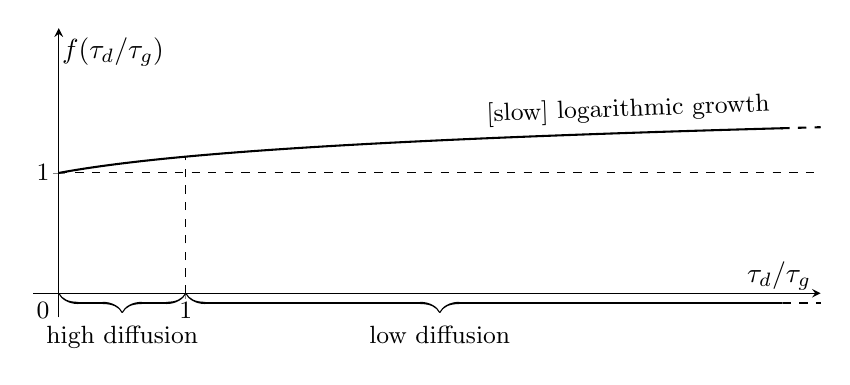
\begin{tikzpicture}[declare function={f(\x)=(9/20)*log10(\x+1)+1;}]

    \pgfmathsetmacro\widthPlot{10}
    \pgfmathsetmacro\heightPlot{10}

    \pgfmathsetmacro\domX{6}
    \pgfmathsetmacro\domY{1.5*f(10)}

    \newcommand\tickSize{8} % Dimensioni delle tacche
    \newcommand\nodeSize{9}
    \pgfmathsetmacro\lineWidth{.75pt}
    
    \pgfmathsetmacro\thresholdDashed{.95}
    \pgfmathsetmacro\yScale{\domY/\domX}

    \def\bracesHeight{7pt}
    \pgfmathsetmacro\tipPos{.4}

    %\begingroup Stili
    \tikzset{
        bracesStyle/.style={
            thick,
            decorate,
            decoration={
                calligraphic brace,
                mirror,
                amplitude=\bracesHeight,
                raise=0pt,
            },
        },
        dashedLine/.style={
            thick,
            dashed,
            yshift=-{.5*\bracesHeight},
        },
        textNodeFont/.style={font=\dimTesto{\nodeSize}},
        textTickFont/.style={font=\dimTesto{\nodeSize}},
        textNodeBraces/.style={textNodeFont,below=8pt},
        textSloped/.style={
            textNodeFont,
            pos=0.75,
            sloped,
            above,
            xshift=10pt,
        },
    }
    \pgfplotsset{
        plotOpt/.style={
            width=\widthPlot cm,
            height=\heightPlot cm,
            clip=false,
            axis lines=middle,
            scale only axis,
            axis x line=center,
            axis y line=center,
            xmin=-.2,xmax=\domX,
            ymin=-.2,ymax=\domY,
            xlabel=$\tau_d/\tau_g$,ylabel=$f(\tau_d/\tau_g)$,
            xtick={1},ytick={1},
            xlabel style={inner ysep=1pt},
            ylabel style={inner xsep=1pt},
            xticklabel style={
                textTickFont,
                inner ysep=1pt,
            },
            yticklabel style={
                textTickFont,
                inner xsep=1pt,
            },
            y post scale=\yScale,
            % axis x line*=bottom,
            % axis y line*=left,
            % xmajorgrids,
            % ymajorgrids,
            % grid style={dashed},
        },
        lineStyleI/.style={
            domain=0:\domX*\thresholdDashed,
            samples=100,
            smooth,
            line width=\lineWidth pt,
        },
        lineStyleF/.style={
            domain={\domX*\thresholdDashed-0.01}:\domX,
            samples=10,
            dashed,
            line width=\lineWidth pt
        },
    }
    %\endgroup

    \begin{axis}[plotOpt]
        \addplot[lineStyleI] {f(x)} node[textSloped] {[slow] logarithmic growth};
        \addplot[lineStyleF] {f(x)};

        \draw[dashed] (0,1) -- (\domX,1);
        \draw[dashed] (1,0) -- (1,{f(1)});

        % Add braces and labels for x-axis segments
        \draw[bracesStyle] (0,0) -- (1,0)
            node[textNodeBraces,midway] {high diffusion};

        \begin{scope}
            \clip(1,0) rectangle ({\thresholdDashed*\domX},-.45);
            \draw[bracesStyle,decoration={aspect=\tipPos}] (1,0) -- (\domX,0)
                node[textNodeBraces,pos=\tipPos] {low diffusion};
        \end{scope}
        \draw[dashedLine] ({\thresholdDashed*\domX},0) -- (\domX,0);

        \node[below left,textTickFont,inner sep=3.2pt] at (axis cs:0,0) {$0$};
    \end{axis}
\end{tikzpicture}

% Vecchio modo, prima che scoprissi «pgfplots», in cui si definita tutto a mano

% \begin{tikzpicture}[declare function={f(\x)=(9/20)*log10(\x+1)+1;},
%                     every node/.style={font=\fontsize{8}{9.6}\selectfont}]
%     % Axes
%     \draw[->] (-0.2,0) -- (6,0) node[above] {$\tau_d$};
%     \draw[->] (0,-0.2) -- (0,2.5) node[right] {$f(\tau_d)$};
    
%     % Logarithmic curve
%     \pgfmathsetmacro{\dashed}{.9}
%     \draw[thick,domain=0:{6*\dashed},smooth,variable=\x] 
%     plot ({\x},{f(\x)});
%     \draw[thick,domain={6*\dashed-0.001}:6,smooth,variable=\x,dashed]
%     plot ({\x},{f(\x)});
    
%     % Constant (low diffusion) line
%     \draw[dashed] (0,1) -- (6,1);
%     \node[left] at (0,1) {$1$};
    
%     % Mark x = 1
%     \pgfmathsetmacro{\x}{1}
%     \draw[dashed] (1,0) -- ({\x},{f(\x)});
%     \node[below] at (1,0) {$1$};
    
%     \pgfmathsetmacro{\x}{5.5}
%     \node[align=center] at
%         ({\x-1.1},{f(\x)+0.3})
%         {[slow] logarithmic growth};
    
%     \pgfmathsetmacro{\bracesHeight}{7pt}
%     % Add braces and labels for x-axis segments
%     \draw[thick,decorate,decoration={calligraphic brace,amplitude=\bracesHeight,mirror,raise=0pt}]
%         (0,0) -- (1,0) node[below=8pt,midway] {high diffusion};

%     \pgfmathsetmacro{\tipPos}{.4}
%     \begin{scope}
%         \clip(1,0) rectangle (5.5,-.7);
%         \draw[thick,
%             decorate,
%             decoration={calligraphic brace,
%                         amplitude=\bracesHeight,
%                         mirror,
%                         raise=0pt,
%                         aspect=\tipPos}
%             ]
%         (1,0) -- (7,0) node[below=8pt,pos=\tipPos] {low diffusion};
%     \end{scope}
%     \pgfmathsetmacro{\bracesHeight}{-{\bracesHeight/2}}
%     \draw[thick,dashed,yshift=\bracesHeight] (5.4,0) -- (6,0);  
% \end{tikzpicture}}
                    \captionsetup{width=0.5\linewidth}
                    \caption{Plot of $f(\tau_d)$ from \eqref{eqConvergenceTimeFunction}.}
                    \label{figftaudForm}
                \end{figure}

        \subsection{Complications}\label{secComplications}

            Modifications are needed to make the models more complex and thus more realistic. In total only three are considered: one for all models and two for the SMO one.

            \subsubsection{Dynamic Laplacian}\label{secComplicationsDynamicLaplacian}

                Ageing is a natural and inevitable process in all our lives, and one crucial way it manifests is in the weakening of the body. Thus, the fact that the Laplacian in \eqref{eqLaplacianMatrix} does not depend on time is in fact a mere simplification.

                But how would the brain depend on time? The answer is not easy and instead of finding it in the literature [if there exists one] we propose two possible behaviours:

                \begin{enumerate}[
                    label=B\arabic*,  % Cambia l'etichetta degli elementi («item») (quella scritta si traduce in 1., 2. ecc.)
                    topsep=7.5pt,	  % Spazio superiore tra testo e lista
                    itemsep=-1pt,	  % Spazio tra gli elementi («item») della lista
                    leftmargin=30pt,  % Spazio tra la lista e il bordo destro del testo
                    rightmargin=20pt, % Spazio tra la lista e il bordo sinistro del testo
                    % \leftmargin + \itemindent = \labelindent + \labelwidth + \labelsep
                    %itemindent=!,
                    % labelindent=30pt,  % Spazio tra il margine sinistro e l'etichetta della lista
                    %labelwidth=!,
                    %labelsep=!
                ]
                    \item\label{bhvUniformDecay} either all edges decay with the same rate in time
                    \item\label{bhvSpecificDecay} or edges decay w.r.t. some quantity: the bigger it is, the faster/slower they decay in time.
                \end{enumerate}

                These reflect how the brain will react in time: if it tries to preserve its form, deeming it optimal, then \ref{bhvUniformDecay} is right; otherwise it will try to maintain certain axons over others based on some quantity like in \ref{bhvSpecificDecay}.

                Between the two \ref{bhvSpecificDecay} is studied simply because it's the most interesting from a theoretical point of view; indeed \ref{bhvUniformDecay} will simply weaken diffusion as \eqref{eqTauD} increases.

                As the control quantity one might propose the distance, but due to the high anisotropy of the brain this is a poor choice. A better one are the entries of the adjacency matrix $\mathbf A$ (Fig. \ref{figMatricesLDA}), which are defined as the ratio of the number of fibres over the average fibre length: $n/l$ \cite{BRCI,BRCII,BRCIII}; therefore, one can arbitrarily assume that the larger $A_{ij}$ is, the greater the brain will try to maintain its associated edge.

                To classify the entries as low/medium/high value the maximum $A_{\max}\approx9.816$, minimum $A_{\min}=0$ and average
                %
                \begin{equation*}
                    \overline A\equiv\frac1{V^2}\sum_{i,j}^VA_{ij}
                    % =\num[scientific-notation=true]{0.1343}
                    \approx0.134
                \end{equation*}
                %
                values of $\mathbf A$ are considered; then the midpoints between $\overline A$-$A_{\max}$ and $\overline A$-$A_{\min}$ defines the thresholds needed to classify the entries:
                %
                \begin{equation}
                    \begin{split}
                        S_{lm}&\equiv\frac{A_{\min}+\overline A}2
                        =\num[scientific-notation=true]{0.0672},\\
                        S_{mh}&\equiv\frac{\overline A+A_{\max}}2
                        \approx4.975,
                    \end{split}
                    \label{eqDecayThresholds}
                \end{equation}
                %
                as illustrated in Fig. \ref{figDecayThresholds}.

                \begin{figure}[htb]
                    \centering
                    \resizebox{\linewidth}{!}{%
                    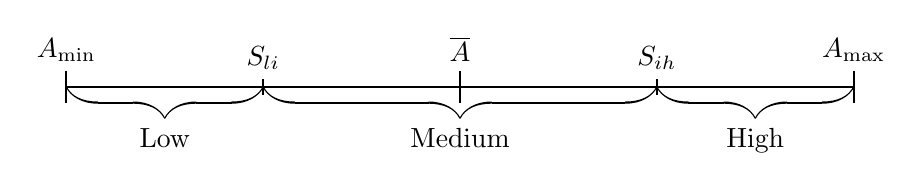
\begin{tikzpicture}
                        \pgfmathsetmacro\LowP{0}
                        \pgfmathsetmacro\MidP{5}
                        \pgfmathsetmacro\HighP{10}
                        \pgfmathsetmacro\Tick{.2}
                        %
                        %
                            % Linea
                        \draw[-,thick] (\LowP,0) -- (\HighP,0);
                        %
                            % Valore minimo
                        \node[above,yshift=\Tick cm] at (\LowP,0) {$A_{\min}$};
                        \draw[-,thick] (\LowP,-\Tick) -- (\LowP,\Tick);
                        %
                            % Valore medio
                        \node[above,yshift=\Tick cm] at (\MidP,0) {$\overline A$};
                        \draw[-,thick] (\MidP,-\Tick) -- (\MidP,\Tick);
                        %
                            % Valore massimo
                        \node[above,yshift=\Tick cm] at (\HighP,0) {$A_{\max}$};
                        \draw[-,thick] (\HighP,-\Tick) -- (\HighP,\Tick);
                        %
                        %
                        \pgfmathsetmacro\Tick{{\Tick/2}}
                        \pgfmathsetmacro\ThresholdLM{{(\LowP+\MidP)/2}}
                        \pgfmathsetmacro\ThresholdMH{{(\MidP+\HighP)/2}}
                        %
                            % Soglia corta-media
                        \node[above,yshift=\Tick cm] at (\ThresholdLM,0) {$S_{li}$};
                        \draw[-,thick] (\ThresholdLM,-\Tick) -- (\ThresholdLM,\Tick);
                        %
                            % Soglia media-lunga
                        \node[above,yshift=\Tick cm] at (\ThresholdMH,0) {$S_{ih}$};
                        \draw[-,thick] (\ThresholdMH,-\Tick) -- (\ThresholdMH,\Tick);
                        %
                        \pgfmathsetmacro\bracesHeight{{\Tick*2+0.2}}
                        %
                        \draw[thick,decorate,
                              decoration={calligraphic brace,
                                          amplitude=\bracesHeight cm,
                                          mirror,raise=0pt}
                        ]
                            (\LowP,0) -- (\ThresholdLM,0)
                            node[below=\bracesHeight cm,midway]
                            {Low};
                        %
                        \draw[thick,decorate,
                              decoration={calligraphic brace,
                                          amplitude=\bracesHeight cm,
                                          mirror,raise=0pt}
                        ]
                            (\ThresholdLM,0) -- (\ThresholdMH,0)
                            node[below=\bracesHeight cm,midway]
                            {Medium};
                        %
                        \draw[thick,decorate,
                              decoration={calligraphic brace,
                                          amplitude=\bracesHeight cm,
                                          mirror,raise=0pt}
                        ]
                            (\ThresholdMH,0) -- (\HighP,0)
                            node[below=\bracesHeight cm,midway]
                            {High};
                    \end{tikzpicture}}
                    \captionsetup{width=\linewidth}
                    \caption{Classifying thresholds.}
                    \label{figDecayThresholds}
                \end{figure}

                \begin{figure}[tb]
                    \centering
                    \resizebox{\linewidth}{!}{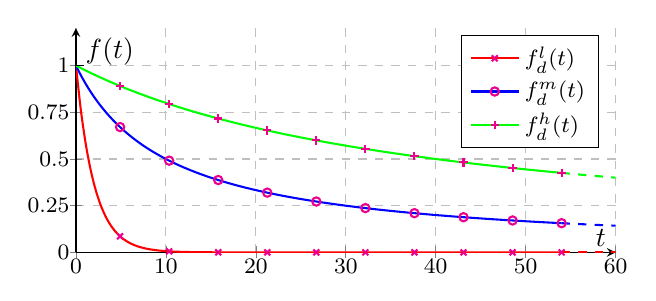
\begin{tikzpicture}[
    declare function={
        f(\x)=exp(-\x/2);
        g(\x)=1/(1+\x/10);
        h(\x)=1/(1+\x/40);
    },
]
    \newcommand\legendSize{8}
    \newcommand\tickSize{8} % Dimensioni delle tacche

    \pgfmathsetmacro\numMarker{10}
    \pgfmathsetmacro\sizeMarker{1.5}
    \pgfmathsetmacro\lineWidth{.75pt}
    
    \pgfmathsetmacro\domainXL{60}
    \pgfmathsetmacro\domainYL{1.2}
    \pgfmathsetmacro\dashed{.9}
    \pgfmathsetmacro\yScale{0.5}

    %\begingroup Stili
    \pgfplotsset{
        plotOpt/.style={
            axis lines=middle,
            xmin=0, xmax=\domainXL,
            ymin=0, ymax=\domainYL,
            xlabel=$t$,
            xlabel style={yshift=-.5mm},
            xtick distance=10,
            xticklabel style={
                font=\dimTesto{\tickSize},
                anchor=north,
                inner sep=0pt,
            },
            ylabel=$f(t)$,
            yticklabel style={
                font=\dimTesto{\tickSize},
                anchor=east,
                inner sep=0pt,
            },
            ytick distance=0.25,
            y post scale=\yScale,
            xmajorgrids,
            ymajorgrids,
            grid style={dashed},
            axis x line*=bottom,
            axis y line*=left,
        },
        legendStyle/.style={
            legend cell align=left,
            align=left,
            legend pos=north east,
            % at={(1,.6)},
            % anchor=east,
            % xshift=-.25cm,
            font=\dimTesto{\legendSize},
            % fill=none,
            % draw=none,
        },
        markOption/.style={
            mark options={solid,magenta},
            mark repeat=\numMarker,
            mark size=\sizeMarker pt,
            mark phase=\numMarker
        },
        markX/.style={markOption,mark=x},
        markO/.style={markOption,mark=o},
        mark+/.style={markOption,mark=+},
        lineOptI/.style={
            domain=0:\domainXL*\dashed,
            samples=100,
            smooth,
            line width=\lineWidth pt,
        },
        lineStyleFfI/.style={lineOptI,color=red,markX},
        lineStyleFgI/.style={lineOptI,color=blue,markO},
        lineStyleFhI/.style={lineOptI,color=green,mark+},
        lineOptF/.style={
            domain={\domainXL*\dashed-0.01}:\domainXL,
            samples=10,
            dashed,
            line width=\lineWidth pt
        },
        lineStyleFfF/.style={lineOptF,color=red},
        lineStyleFgF/.style={lineOptF,color=blue},
        lineStyleFhF/.style={lineOptF,color=green},
    }
    %\endgroup

    \begin{axis}[plotOpt,legend style=legendStyle]
        \addplot[lineStyleFfI] {f(x)};
        \addlegendentry{$f_d^l(t)$}
        \addplot[lineStyleFgI] {g(x)};
        \addlegendentry{$f_d^m(t)$}                    
        \addplot[lineStyleFhI] {h(x)};
        \addlegendentry{$f_d^h(t)$}

        \addplot[lineStyleFfF] {f(x)};
        \addplot[lineStyleFgF] {g(x)};
        \addplot[lineStyleFhF] {h(x)};

        \draw[dashed] (0,1) -- (1,1);

        % node[above] at ({0.2*\domainXL},{f(0.2*\domainXL)}) {$f_d^l(t)$};
        % node[above] at ({0.2*\domainXL},{f(0.2*\domainXL)}) {$f_d^l(t)$};
        % node[above] at ({0.5*\domainXL},{g(0.5*\domainXL)}) {$f_d^m(t)$};
        % node[above] at ({0.5*\domainXL},{g(0.5*\domainXL)}) {$f_d^m(t)$};
        % node[above] at ({0.75*\domainXL},{h(0.75*\domainXL)}) {$f_d^h(t)$};
        % node[above] at ({0.75*\domainXL},{h(0.75*\domainXL)}) {$f_d^h(t)$};
    \end{axis}
\end{tikzpicture}


% Vecchia versione
% \pgfmathsetmacro\xScale{0.1}
% \pgfmathsetmacro\yScale{2}
% \begin{tikzpicture}[xscale=\xScale,
%                     yscale=\yScale,
%                     declare function={
%                         f(\x)=exp(-\x/2);
%                         g(\x)=1/(1+\x/10);
%                         h(\x)=1/(1+\x/40);
%                         },
%                     every node/.style={font=\fontsize{8}{9.6}\selectfont}]

%     \pgfmathsetmacro\dashed{.9}
%     \pgfmathsetmacro\DomainXL{70}
%     \pgfmathsetmacro\DomainYL{1.2}

%     % Axes
%     \draw[->] (-{.2/\xScale},0) -- (\DomainXL,0)
%         node[above] {$t$};
%     \draw[->] (0,-{.2/\yScale}) -- (0,\DomainYL)
%         node[right] {$f(t)$};
%     \draw[dashed] (0,1) -- (\DomainXL,1);
%     \node[left] at (0,1) {$1$};

%     \pgfmathsetmacro\DomainXL{\DomainXL*.98}

%     % First Decay function
%     \draw[thick,
%             domain=0:{\DomainXL*\dashed},
%             smooth,
%             variable=\x
%         ] 
%     plot ({\x},{f(\x)});
%     \draw[thick,
%             domain={\DomainXL*\dashed-0.001}:\DomainXL,
%             smooth,
%             variable=\x,
%             dashed
%         ]
%     plot ({\x},{f(\x)});
%     \node[above]
%         at ({\DomainXL*0.2},{f(\DomainXL*0.2)})
%         {$f^l_d(t)$};

%     % Second Decay function
%     \draw[thick,
%             domain=0:{\DomainXL*\dashed},
%             smooth,
%             variable=\x] 
%     plot ({\x},{g(\x)});
%     \draw[thick,
%             domain={\DomainXL*\dashed-0.001}:\DomainXL,
%             smooth,
%             variable=\x,
%             dashed]
%     plot ({\x},{g(\x)});
%     \node[above]
%         at ({\DomainXL*0.5},{g(\DomainXL*0.5)})
%         {$f^m_d(t)$};

%     % Third Decay function
%     \draw[thick,
%             domain=0:{\DomainXL*\dashed},
%             smooth,
%             variable=\x] 
%     plot ({\x},{h(\x)});
%     \draw[thick,
%             domain={\DomainXL*\dashed-0.001}:\DomainXL,
%             smooth,
%             variable=\x,
%             dashed]
%     plot ({\x},{h(\x)});
%     \node[above]
%         at ({\DomainXL*0.75},{h(\DomainXL*0.75)})
%         {$f^h_d(t)$};
% \end{tikzpicture}}
                    \captionsetup{width=0.5\linewidth}
                    \caption{Decay functions.}
                    \label{figDecayFunctions}
                \end{figure}

                In total the number of low/medium/high value edges are \num{5785}, \num{1094} and \num{10} respectively, which sum to $83^2$ as expected. With all this, $\mathbf A(t)$ is defined as follows
                %
                \begin{equation}
                    \newcommand\vspcR{2pt}
                    A_{ij}(t)\equiv
                    \left\{
                    \begin{alignedat}{2}
                        &A_{ij}f_d^l(t)\quad&\text{if }&A_{\min}\le A_{ij}<S_{lm}\\[\vspcR]
                        &A_{ij}f_d^m(t)\quad&\text{if }&S_{lm}  \le A_{ij}<S_{mh}\\[\vspcR]
                        &A_{ij}f_d^h(t)\quad&\text{if }&S_{mh}  \le A_{ij}<A_{\max}
                    \end{alignedat}
                    \right.
                    \label{eqTimeDependentA}
                \end{equation}
                %
                where the three decaying functions are
                %
                \begin{equation}
                    f_d^l(t)\equiv\exp\left[-\frac t2\right],\;\;\;
                    f_d^m(t)\equiv\frac1{1+\frac t{10}},\;\;\;
                    f_d^h(t)\equiv\frac1{1+\frac t{40}},
                    % \begin{gathered}
                    %     f_{dl}(t)=\exp\left[-\frac t2\right],\quad
                    %     f_{dm}(t)=\frac1{1+\frac t{10}},\\
                    %     f_{dh}(t)=\frac1{1+\frac t{40}}.
                    % \end{gathered}
                    \label{eqDecayingFunctions}
                \end{equation}
                %
                shown in Fig. \ref{figDecayFunctions}.

                Afterwards, $\mathbf L$ is defined exactly as \eqref{eqLaplacianMatrix}:
                %
                \begin{equation}
                    \mathbf L(t)\equiv\rho(\mathbf D(t)-\mathbf A(t))=\rho\boldsymbol{\mathcal L}(t),
                    \label{eqDynamicLaplacianMatrix}
                \end{equation}
                %
                but with $\mathbf D(t)\equiv\diag(\mathbf A(t)\boldsymbol1)$.

                It's noteworthy to emphasize that the kinematics described by \eqref{eqTimeDependentA} is purely theoretical and based on the assumption that the low value edges decay very rapidly (exponential decay), whereas those medium and high value are more resistant (hyperbolic decay).

            \subsubsection{Accumulation}\label{secComplicationsAccumulation}

                In \SMOcontinuous{} it's possible to assume the last $L$-th polymer cannot be cleared and accumulate in time, leading to brain damages; this can be taken into account by setting $\mu_L=0$ instead of $\mu_L=\mu$ in \ref{hypSMOModelClearance}.

            \subsubsection{Size-dependency}\label{secComplicationsSizeDependency}

                Still within \SMOcontinuous{}, it's possible to assume that both diffusion and clearance rate depend on the polymer size; this is sensible as the larger a polymer is, the less is able to diffuse and the longer it takes to break it down.

                For diffusion, \ref{hypSMOModelDiffusion} can be changed so that the diffusion coefficient $\mathbf D_i$ of the $i$-th polymer scales approximately as a power of its molecular weight which is proportional to the polymer size: \cite[(23) on p. 5]{Goriely2019}
                %
                \begin{equation}
                    \mathbf D_i\equiv i^{-\eta}\mathbf D
                    \quad\implies\quad
                    \mathbf L_i\equiv i^{-\eta}\mathbf L,
                    \label{eqSizeDependentDiffusion}
                \end{equation}
                %
                where $\eta=0.5$.

                For clearance, \ref{hypSMOModelClearance} can be modified by setting $\mu_i=\mu/i$; in this way, the larger the polymer is, the slower it's clear\-ed. This last change actually breaks mass conservation in \eqref{eqMassConservation} which becomes \cite[(47) on p. 8]{Goriely2019}
                %
                \begin{equation}
                    \derT\TotM t=\gamma-\mu\TotP,
                    \label{eqPTotEquation}
                \end{equation}
                %
                where $\TotP\equiv\sum_{i=1}^Lc_i=c_1+P=m+P$, so mass is expected to grow even if $\TotM(0)=\gamma/\mu$. The same result [but not \eqref{eqPTotEquation}] is true, to a lesser extent, with the previous complication in which only $\mu_L=0$ is different.

%%%
%%%
%%%

    \section{Settings and results}\label{secResultsComparisons}

        In this section the parameters and initial conditions of the models are set, then the results are discussed by comparing the base models with and without complications.

        \subsection{Settings}\label{secSettings}

            In few words, all parameters come from \cite{Fornari2019}; \SMOdiscrete{} has been tested with those taken from \cite{Goriely2019} as well. In particular, two settings are shared between all models:

            \begin{itemize}[%
                topsep=7.5pt,	  % Spazio superiore tra testo e lista
                itemsep=-2pt,	  % Spazio tra gli elementi («item») della lista
                leftmargin=30pt,  % Spazio tra la lista e il bordo destro del testo
                rightmargin=0pt,  % Spazio tra la lista e il bordo sinistro del testo
                %itemindent=!,
                % labelindent=30pt, % Spazio tra il margine sinistro e l'etichetta della lista
                %labelwidth=!,
                %labelsep=!
                % \leftmargin + \itemindent = \labelindent + \labelwidth + \labelsep
            ]
                \item the infected nodes, \ie{} where the initial toxic conditions are set (§ \ref{secDiscreteModels}), are those in the entorhinal cortex ($q=2$) in the Limbic system, shown in Fig. \ref{figInfectedNodes};
                \item $\rho$ is chosen such that
                %
                \begin{equation}
                    \rho\equiv\Vert\mathbf L\Vert_2^{-1}=0.0219
                    \ \ \implies\ \ \tau_d=1.
                    \label{eqRhoValueCaseStudies}
                \end{equation}
            \end{itemize}

            \begin{figure}[tb]
                \newcommand\dimImm{.75\linewidth}
                \centering
                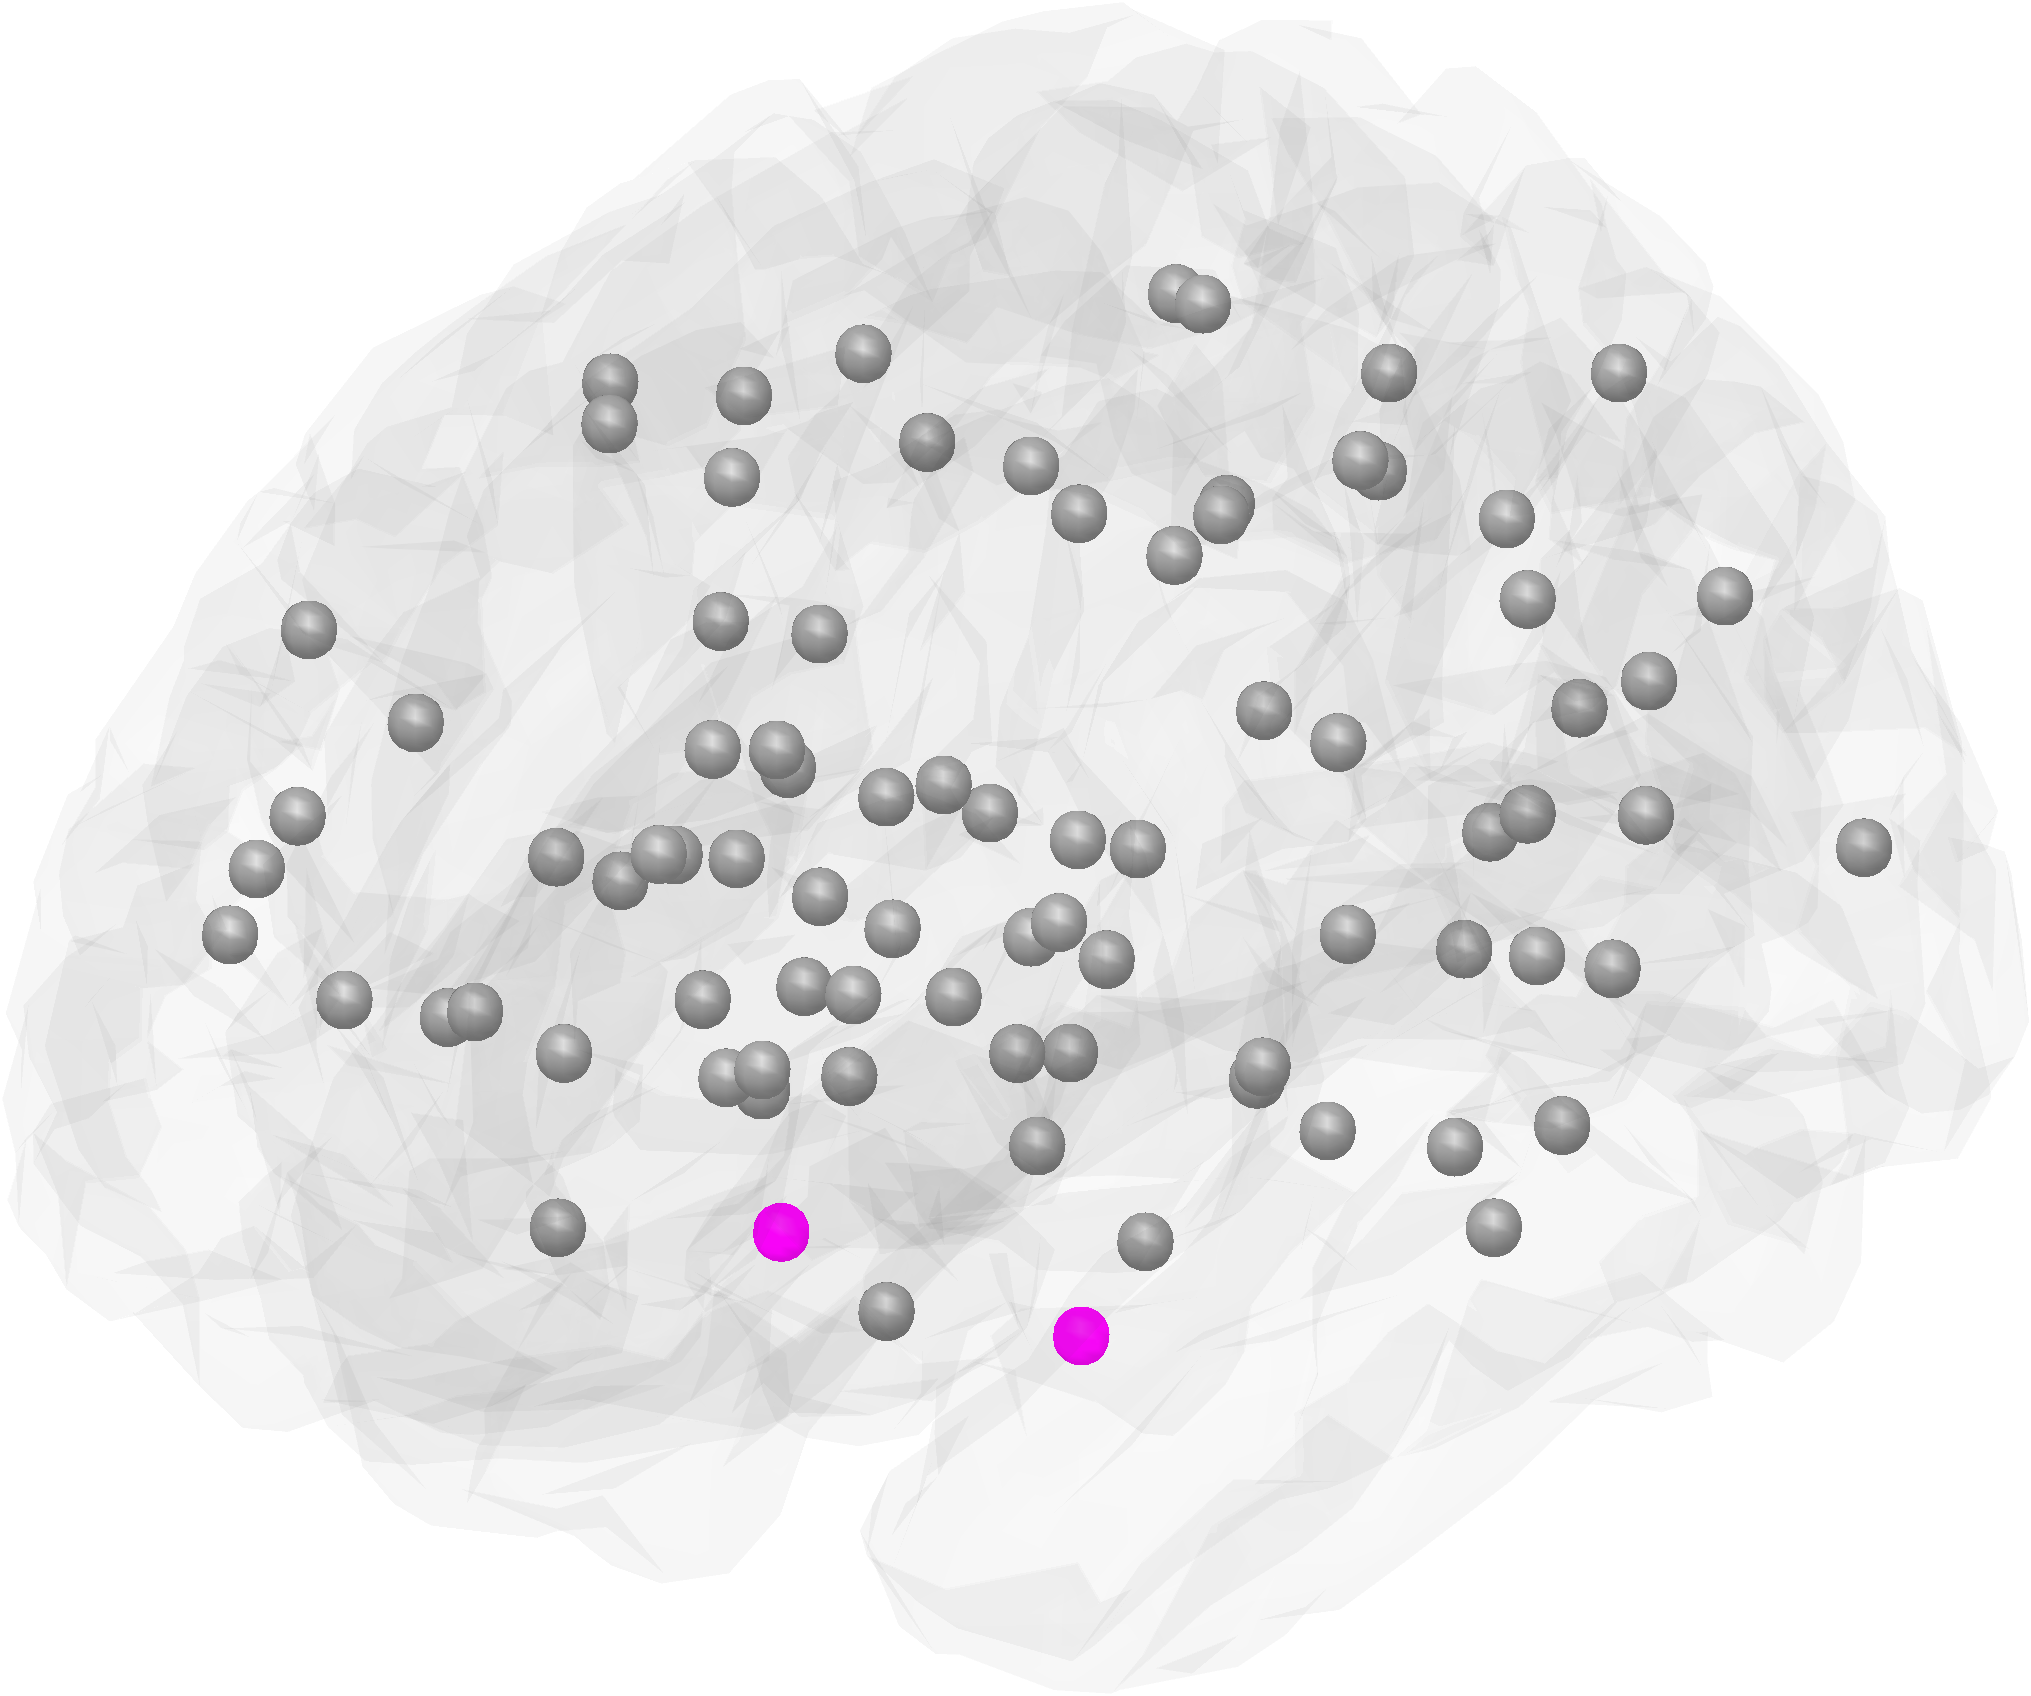
\includegraphics[width=\dimImm]{../Figure/nodiInfettiCervello.png}
                \caption{Entorhinal infected nodes coloured magenta.}
                \label{figInfectedNodes}
            \end{figure}

            In conclusion to this section, some remarks are necessary in regard to all parameters.

            \subsubsection{FK model}\label{secSettingsFK}

                The \FKdiscrete{} settings are the following:

                \begin{itemize}[%
                    topsep=7.5pt,	  % Spazio superiore tra testo e lista
                    itemsep=-2pt,	  % Spazio tra gli elementi («item») della lista
                    leftmargin=20pt,  % Spazio tra la lista e il bordo destro del testo
                    rightmargin=0pt,  % Spazio tra la lista e il bordo sinistro del testo
                    %itemindent=!,
                    % labelindent=30pt, % Spazio tra il margine sinistro e l'etichetta della lista
                    %labelwidth=!,
                    %labelsep=!
                    % \leftmargin + \itemindent = \labelindent + \labelwidth + \labelsep
                ]
                    \item the parameter takes value
                    %
                    \begin{equation}
                        \alpha=\qty{0.5}{\per\year},
                        \label{eqFKParameters}
                    \end{equation}
                    %
                    where $\unit{\year}$ stands for \textit{annus}, meaning year in Latin. Of course, [tropical] years aren't a fundamental dimension, although they can be converted in seconds, as suggested by the SI \cite{ISO80k3,GUISUThompson2008}, with
                    %
                    \begin{equation}
                        \qty{1}{\year}\approx
                        \qty{365.24220}{d}\approx
                        \qty[scientific-notation=true]{31556926}{\second};
                        % 1\ \Year\approx 365.24220\ \text{d}\approx 31\ 556\ 926\ \text{s}.
                        \label{eqConversionYearsSeconds}
                    \end{equation}
                    %
                    \item $\tau_g$ and $T_c$ values, from \cref{eqTauGFK,eqConvergenceTimeFunction} respectively, can be found in Tab. \ref{tabTimeDataSettings};

                    \item the initial toxic concentration is $c_0=\num{0.1}$;

                    \item the Euler implicit method in \eqref{eqUpdateRuleEI} is considered with $\Delta t=\qty{0.4}{\year}$ and $T=\qty{30}{\year}$.
                \end{itemize}

            \subsubsection{HD model}\label{secSettingsHD}

                The \HDdiscrete{} settings are the following:

                \begin{itemize}[%
                    topsep=7.5pt,	  % Spazio superiore tra testo e lista
                    itemsep=-2pt,	  % Spazio tra gli elementi («item») della lista
                    leftmargin=20pt,  % Spazio tra la lista e il bordo destro del testo
                    rightmargin=0pt,  % Spazio tra la lista e il bordo sinistro del testo
                    %itemindent=!,
                    % labelindent=30pt, % Spazio tra il margine sinistro e l'etichetta della lista
                    %labelwidth=!,
                    %labelsep=!
                    % \leftmargin + \itemindent = \labelindent + \labelwidth + \labelsep
                ]
                    \item the parameters are
                    %
                    \begin{equation}
                        \newcommand\hspcC{\qquad}
                        \begin{alignedat}{2}
                            \gamma&=\qty{1}{\molarity\per\year},&\hspcC
                            \kappa&=\qty{0.5}{\per\molarity\per\year},\\
                            \mu_h&=\qty{0.5}{\per\year},&\hspcC
                            \mu_m&=\qty{0.5}{\per\year},
                            % \gamma&=1\ \Molarity\cdot\Year\PowerMinOne,&\hspcC
                            % \kappa&=0.5\ \Molarity\PowerMinOne\cdot\Year\PowerMinOne,\\
                            % \mu_h&=0.5\ \Year\PowerMinOne,&\hspcC
                            % \mu_m&=0.5\ \Year\PowerMinOne.
                        \end{alignedat}
                        \label{eqHDParameters}
                    \end{equation}
                    %
                    where $\unit{\molarity}$ is molar concentration defined in SI units as \cite{PMCOxtoby2016} \[\unit{\molarity}=\unit{\mole/\metre\cubed};\]

                    \item $\tau_g$ and $T_c$ values, from \cref{eqTauGHD,eqConvergenceTimeFunction} respectively, can be found in Tab. \ref{tabTimeDataSettings};

                    \item the asymptotic values from \eqref{eqHDEP} are
                    %
                    \[
                        c_{h,2}^\infty=\qty1{\molarity},
                        \quad\text{and}\quad
                        c_{m,2}^\infty=\qty1{\molarity};
                    \]
                    %
                    \item the initial healthy concentration is $c_{h,0}=\qty{2}{\molarity}$ while the initial toxic one is $c_{m,0}=\qty{0.1}{\molarity}$;

                    \item the Euler implicit method in \eqref{eqUpdateRuleEI} is considered with $\Delta t=\qty{0.4}{\year}$ and $T=\qty{30}{\year}$.
                \end{itemize}

            \subsubsection{SMO model}\label{secSettingsSMO}

                \begin{table}[tb]
                    \sisetup{scientific-notation=false}
                    %
                    \newcommand\halfHeight{.1cm}
                    \newcommand\wCol{1cm}
                    \newcommand\hRow{\halfHeight}
                    \setlength\extrarowheight{\halfHeight}
                    \newcommand\sepCol{\hspace{1cm}}
                    %
                    \centering
                    \begin{NiceTabular}{
                        wc{\wCol}|
                        S[
                            table-format=1.2e2,
                            exponent-mode=scientific,
                            retain-zero-exponent=true,
                        ]
                        S[
                            table-format=1e1,
                            exponent-mode=scientific,
                            retain-zero-exponent=true,
                        ]
                        S[
                            table-format=1e1,
                            exponent-mode=scientific,
                            retain-zero-exponent=true,
                        ]
                        S
                    }[
                        % corners,
                        %hvlines-except-borders,
                        % hvlines,
                        rounded-corners,
                        notes/para=true,
                    ]
                        \CodeBefore
                            % \chessboardcolors{red!15}{blue!15}
                            % \chessboardcolors{black!15!white}{}
                            \rowcolors{1}{black!5!white}{black!15!white}
                        \Body
                        &{$\rho$}&{$\tau_d$ [\unit{\year}]}
                        &{$\tau_g$ [\unit{\year}]}&{$T_c$[\unit{\year}]}\\[\hRow]\hline
                        {\FKdiscrete} &0.0219&1&2&21.58\\[\hRow]
                        {\HDdiscrete} &0.0219&1&2&21.58\\[\hRow]
                        {\SMOdiscrete}&0.0219&1&2&21.58\\[\hRow]
                    \end{NiceTabular}
                    \caption{Constant $\rho$, timescales and convergence time of the case studies.}
                    \label{tabTimeDataSettings}
                \end{table}

                The \SMOdiscrete{} settings are the following:

                \begin{itemize}[%
                    topsep=7.5pt,	  % Spazio superiore tra testo e lista
                    itemsep=-2pt,	  % Spazio tra gli elementi («item») della lista
                    leftmargin=20pt,  % Spazio tra la lista e il bordo destro del testo
                    rightmargin=0pt,  % Spazio tra la lista e il bordo sinistro del testo
                    %itemindent=!,
                    % labelindent=30pt, % Spazio tra il margine sinistro e l'etichetta della lista
                    %labelwidth=!,
                    %labelsep=!
                    % \leftmargin + \itemindent = \labelindent + \labelwidth + \labelsep
                ]
                    \item the parameters are
                        %
                        \begin{equation}
                            \newcommand\hspcC{\quad}
                            \begin{alignedat}{2}
                                \gamma&=\qty{1}{\molarity\per\year},&\hspcC
                                \mu&=\qty{0.5}{\per\year},\\
                                a&=\qty{10}{\per\molarity\per\year},&\hspcC
                                f&=\qty{0.096}{\per\year},\\
                                \kappa&=\qty{1.6e-4}{\per\molarity\per\year},&\hspcC
                                L&=50;
                                % \kappa=1.6\times10^{-4}\
                                % \Molarity\PowerMinOne\cdot\Year\PowerMinOne.
                                % \gamma&=1\ \Molarity\cdot\Year\PowerMinOne,&\hspcC
                                % \mu&=0.5\ \Year\PowerMinOne,\\
                                % a&=10\ \Molarity\PowerMinOne\cdot\Year\PowerMinOne,&\hspcC
                                % f&=0.048\ \Year\PowerMinOne.
                            \end{alignedat}
                            \label{eqSMOParameters}
                        \end{equation}
                        %
                    \item $\tau_g$ and $T_c$ values, from \cref{eqTauGSMO,eqConvergenceTimeFunction} respectively, can be found in Tab. \ref{tabTimeDataSettings};

                    \item numerically the asymptotic values from \cref{eqMInfValue,eqPInfValue,eqmInfEstimateEquation} (with $\varphi$ from \eqref{eqDiscreteAverageNucleation}) are
                    %
                    %
                    \begin{equation*}
                        \begin{split}
                            \mInf&=\qty{0.6708}{\molarity},\\
                            \MInf&=\qty{1.3292}{\molarity},\\
                            \PInf&=\qty{0.0991}{\molarity};
                        \end{split}
                    \end{equation*}
                    %
                    %
                    \item the initial healthy concentration is $c_{1,0}=\qty2{\molarity}=\gamma/\mu$;
                    \item the Euler explicit method in \eqref{eqUpdateRuleEE} is considered with $\Delta t=\qty{0.04}{\year}$, to ensure its stability, and $T=\qty{60}{\year}$.
                \end{itemize}

            \subsubsection{Disclaimer}\label{secDisclaimer}

                The data in \cite{Fornari2019} have three majors problems:

                \begin{enumerate}[
                    label=P\arabic*,  % Cambia l'etichetta degli elementi («item») (quella scritta si traduce in 1., 2. ecc.)
                    topsep=7.5pt,       % Spazio superiore tra testo e lista
                    itemsep=-1pt,	    % Spazio tra gli elementi («item») della lista
                    leftmargin=30pt,    % Spazio tra la lista e il bordo destro del testo
                    rightmargin=20pt,	% Spazio tra la lista e il bordo sinistro del testo
                    % \leftmargin + \itemindent = \labelindent + \labelwidth + \labelsep
                    %itemindent=!,
                    % labelindent=30pt, 	% Spazio tra il margine sinistro e l'etichetta della lista
                    %labelwidth=!,
                    %labelsep=!
                ] % Per il significato di queste impostazioni si veda p. 3 della documentazione «enumitem»
                    \item\label{problemDimension} the authors don't mention their dimensions which from the plots we assumed to be in $\unit{\year}$;
                    \item\label{problemReference} the authors don't reference any studies from which their parameters are taken;
                    \item\label{problemLaplacian} the authors do not provide the Laplacian used.
                \end{enumerate}

                To solve \ref{problemLaplacian} we could build the Laplacian or take another already built; as written in § \ref{secSpatialDiscretization}, we have chosen to follow the latter by considering the one in \cite{Goriely2019}, which is, however, not provided directly in the publication but in its preprint \cite{Goriely2019_L}.

                Instead, \ref{problemReference} suggests the parameters are purely theoretical which seems to be the case even in \cite{Goriely2019}; in both papers, however, this is only implied by context and not explicitly written. For this reason we advise considering all previous parameters as merely theoretical.

                It's then to no-one's surprise the results in \cite{Fornari2019} have unfortunately not been reproduced correctly:

                \begin{itemize}[%
                    topsep=7.5pt,     % Spazio superiore tra testo e lista
                    itemsep=-2pt,	  % Spazio tra gli elementi («item») della lista
                    leftmargin=20pt,  % Spazio tra la lista e il bordo destro del testo
                    rightmargin=0pt,  % Spazio tra la lista e il bordo sinistro del testo
                    % \leftmargin + \itemindent = \labelindent + \labelwidth + \labelsep
                    %itemindent=!,
                    % labelindent=30pt, 	% Spazio tra il margine sinistro e l'etichetta della lista
                    %labelwidth=!,
                    %labelsep=!
                ] % Per il significato di queste impostazioni si veda p. 3 della documentazione «enumitem»
                    \item the FK and HD simulations have the same convergence time but they manifest a different dynamic in which their spreading is clockwise:
                    %
                    \begin{subequations}
                        \newcommand\verso{$\;\to\;$}
                        \begin{align}
                            \text{temporal\verso frontal\verso parietal\verso occipital},
                            \tag{cw}\label{eqClockwiseSpreading}\\
                    \intertext{starting from the entorhinal cortex, whereas ours is anticlockwise, \ie{} it reverses the last three regions:}
                            \text{temporal\verso occipital\verso parietal\verso frontal}.
                            \tag{acw}\label{eqAntiClockwiseSpreading}
                        \end{align}
                    \end{subequations}
                    %
                    \item the SMO simulation has both a different spreading and convergence time about \qty{30}{\year} slower.
                \end{itemize}
                    %
                    %   Discarded code as the two equations are not aligned
                    %
                    % With clockwise we mean the spreading, in order of time,
                    %
                    % \begin{equation}
                    %     \text{temporal$\to$frontal$\to$parietal$\to$                    occipital},
                    %     \tag{cw}\label{eqClockwiseSpreading}
                    % \end{equation}
                    %
                    % starting from the entorhinal nodes; meanwhile anticlockwise reverses the last three regions:
                    %
                    % \begin{equation}
                    %     \text{temporal$\to$occipital$\to$parietal$\to$frontal}.
                    %     \tag{acw}\label{eqAntiClockwiseSpreading}
                    % \end{equation}
                Nevertheless, these discrepancies are not crucial in this paper as we are only interested in comparing the base and modified models, which is possible even only on theoretical grounds.

        \subsection{Results}\label{secResults}

            The simulation results using the parameters of the previous section are discussed first for \FKdiscrete{} and \HDdiscrete{} at once, and then for \SMOdiscrete{}.

            All simulations have been carried out with MATLAB software version «24.2.0.2923080 (R2024b) Update 6», alongside Optimization Toolbox version 24.2.

            % \begin{figure*}[t]
            %     \centering
            %     \resizebox{\textwidth}{!}{% This file was created by matlab2tikz.
%
%The latest updates can be retrieved from
%  http://www.mathworks.com/matlabcentral/fileexchange/22022-matlab2tikz-matlab2tikz
%where you can also make suggestions and rate matlab2tikz.

% This code was later modified by Valerio Taralli

\begin{tikzpicture}

    \definecolor{mycolor1}{rgb}{1.00000,0.54510,0.00000}%
    \definecolor{mycolor2}{rgb}{0.50588,0.00000,0.49804}%
    \definecolor{mycolor3}{rgb}{0.00000,0.74510,0.00000}%
    \definecolor{mycolor4}{rgb}{0.50196,0.50196,0.50196}%

    %

    \pgfmathsetmacro\fSizeTitle{14.4}
    \pgfmathsetmacro\baseline{\fSizeTitle*1.2}
    \newcommand\tSizeTitle{\fontsize{\fSizeTitle pt}{\baseline pt}\selectfont}

    \pgfmathsetmacro\fSizeLabel{10.95}
    \pgfmathsetmacro\baseline{\fSizeLabel*1.2}
    \newcommand\tSizeLabel{\fontsize{\fSizeLabel pt}{\baseline pt}\selectfont}
    
    \pgfmathsetmacro\fSizeLegend{8}
    \pgfmathsetmacro\baseline{\fSizeLegend*1.2}
    \newcommand\tSizeLegend{\fontsize{\fSizeLegend pt}{\baseline pt}\selectfont}

    \pgfmathsetmacro\widthCurves{10}
    \pgfmathsetmacro\heightCurves{.6*\widthCurves}
    \pgfmathsetmacro\lineWidth{.75pt}

    \begin{groupplot}[
                    group style={
                                group name=FKHD,
                                group size=2 by 4,
                                horizontal sep=.5cm,
                                vertical sep=.5cm,
                                xlabels at=edge bottom,
                                ylabels at=edge left,
                                xticklabels at=edge bottom,
                                yticklabels at=edge left,
                                },
                    width=\widthCurves cm,% 10.45in
                    height=\heightCurves cm,% height=6.328in,
                    xmin=0,xmax=30,
                    xlabel={\selezionaLingua{Tempo [anni]}{Time [years]}},
                    xlabel style={
                                font=\color{white!15!black}\tSizeLabel,
                                % at={(ticklabel cs:1.0)},
                                % anchor=east,
                                % yshift=-.3cm,
                                },
                    ymin=0,ymax=1,
                    ylabel={\selezionaLingua{Concentrazione}{Concentration} [\%]},
                    ylabel style={
                                font=\color{white!15!black}\tSizeLabel,
                                % at={(ticklabel cs:1.0)},
                                % anchor=east,
                                % yshift=.3cm,
                                },
                    ytick distance=0.1,
                    % axis background/.style={fill=white},
                    axis x line*=bottom,
                    axis y line*=left,
                    xmajorgrids,
                    ymajorgrids,
                    grid style={dashed},
    ]
        % FKS
        \nextgroupplot[
                        title style={font=\bfseries\tSizeTitle},
                        title={\selezionaLingua{Modello \FKdiscrete{}}{\FKdiscrete{} model}},
                        legend style={legend cell align=left,
                                    align=left,
                                    legend pos=north west,
                                    draw=white!15!black,
                                    font=\tSizeLegend,
                                    fill=none,
                                    draw=none,
                                    },
                    ]
        %\begingroup
        \addplot [color=black,dashed,line width=\lineWidth]
        table[row sep=crcr]{%
        0	0.00240963855421687\\
        0.4	0.00292466694502703\\
        0.8	0.00353051798613887\\
        1.2	0.00423575301794363\\
        1.6	0.00504723498398421\\
        2	0.00596943575665791\\
        2.4	0.00700393571996942\\
        2.8	0.00814928980826412\\
        3.2	0.00940141280649278\\
        3.6	0.0107545683067739\\
        4	0.0122029430445444\\
        4.4	0.013742681545431\\
        4.8	0.0153741809372758\\
        5.2	0.0171044273808024\\
        5.6	0.018949196354367\\
        6	0.0209350192977247\\
        6.4	0.0231009077937727\\
        6.8	0.0254998949309883\\
        7.2	0.0282004848774382\\
        7.6	0.0312880926644489\\
        8	0.0348665130872544\\
        8.4	0.0390593910331643\\
        8.8	0.0440115859207532\\
        9.2	0.0498902386294065\\
        9.6	0.0568852662403863\\
        10	0.0652089321886856\\
        10.4	0.075094070495834\\
        10.8	0.0867904876309496\\
        11.2	0.100559034469464\\
        11.6	0.11666285391722\\
        12	0.135355400497225\\
        12.4	0.156865041896579\\
        12.8	0.181376436304854\\
        13.2	0.209009461484802\\
        13.6	0.239797230658633\\
        14	0.273665563845014\\
        14.4	0.31041699072444\\
        14.8	0.349722666287717\\
        15.2	0.391125208621918\\
        15.6	0.434054267035927\\
        16	0.477854688439047\\
        16.4	0.521824851858232\\
        16.8	0.565260681986777\\
        17.2	0.607499646098651\\
        17.6	0.647959070337275\\
        18	0.686164370106723\\
        18.4	0.721764866881444\\
        18.8	0.754537130166669\\
        19.2	0.78437764431403\\
        19.6	0.811287703588204\\
        20	0.835353742070593\\
        20.4	0.856725998021404\\
        20.8	0.875597777062596\\
        21.2	0.892186863129925\\
        21.6	0.906719983869656\\
        22	0.919420726659844\\
        22.4	0.93050092051795\\
        22.8	0.940155222610056\\
        23.2	0.948558453341951\\
        23.6	0.95586510062275\\
        24	0.962210360831135\\
        24.4	0.967712101522667\\
        24.8	0.972473212389165\\
        25.2	0.976583938997425\\
        25.6	0.980123942011573\\
        26	0.983163964488453\\
        26.4	0.985767099239845\\
        26.8	0.987989716732996\\
        27.2	0.989882143198024\\
        27.6	0.991489178331879\\
        28	0.992850524801953\\
        28.4	0.99400117867426\\
        28.8	0.994971808297807\\
        29.2	0.995789132675063\\
        29.6	0.996476299730123\\
        30	0.997053259343476\\
        };
        \addlegendentry{\selezionaLingua{Rete}{Network}}

        \addplot [color=mycolor3,line width=\lineWidth]
        table[row sep=crcr]{%
        0	0\\
        0.4	7.04171308035969e-05\\
        0.8	0.000167204870158116\\
        1.2	0.000297593640187517\\
        1.6	0.000470390013802762\\
        2	0.000696245355284452\\
        2.4	0.000987971062313396\\
        2.8	0.0013609184425676\\
        3.2	0.00183344759533764\\
        3.6	0.00242751517133566\\
        4	0.00316941440823425\\
        4.4	0.00409070162786215\\
        4.8	0.00522934121508573\\
        5.2	0.0066310960862461\\
        5.6	0.00835118270409855\\
        6	0.0104561978995399\\
        6.4	0.0130263069503896\\
        6.8	0.0161576549880046\\
        7.2	0.0199649221440306\\
        7.6	0.0245838816770031\\
        8	0.0301737350345202\\
        8.4	0.0369188864319309\\
        8.8	0.0450296858239076\\
        9.2	0.0547415269702302\\
        9.6	0.0663115655831689\\
        10	0.0800122689302961\\
        10.4	0.0961210876435003\\
        10.8	0.114905823369987\\
        11.2	0.136605802613272\\
        11.6	0.161409749715755\\
        12	0.189432177122903\\
        12.4	0.220690968896398\\
        12.8	0.255089347297504\\
        13.2	0.292405334190111\\
        13.6	0.332291046146569\\
        14	0.374282810572877\\
        14.4	0.41782147487804\\
        14.8	0.462280801851337\\
        15.2	0.507000837513125\\
        15.6	0.551322761370546\\
        16	0.594621937573151\\
        16.4	0.636336489355429\\
        16.8	0.675989495718517\\
        17.2	0.713203702148864\\
        17.6	0.747708388248447\\
        18	0.779338741331604\\
        18.4	0.808028728216808\\
        18.8	0.833798971667276\\
        19.2	0.856741436627096\\
        19.6	0.877002761951682\\
        20	0.894767852410365\\
        20.4	0.910244952626059\\
        20.8	0.923652965639442\\
        21.2	0.935211348638105\\
        21.6	0.945132577493601\\
        22	0.953616942421616\\
        22.4	0.960849312865438\\
        22.8	0.966997468289605\\
        23.2	0.972211606252418\\
        23.6	0.976624685770879\\
        24	0.980353324229183\\
        24.4	0.983499027729342\\
        24.8	0.986149590853921\\
        25.2	0.988380549116344\\
        25.6	0.990256605153449\\
        26	0.991832978589798\\
        26.4	0.993156650736144\\
        26.8	0.994267490329762\\
        27.2	0.995199256770219\\
        27.6	0.995980483956158\\
        28	0.996635251872164\\
        28.4	0.99718385528054\\
        28.8	0.997643379824385\\
        29.2	0.99802819597514\\
        29.6	0.998350380868111\\
        30	0.998620077379601\\
        };
        \addlegendentry{\selezionaLingua{Temporale}{Temporal}}

        \addplot [color=black!20!red,line width=\lineWidth]
        table[row sep=crcr]{%
        0	0\\
        0.4	7.45220646300966e-07\\
        0.8	2.66053818596208e-06\\
        1.2	6.33256066900085e-06\\
        1.6	1.25599498691129e-05\\
        2	2.241734705516e-05\\
        2.4	3.73363879315073e-05\\
        2.8	5.92082605309713e-05\\
        3.2	9.05135077117992e-05\\
        3.6	0.000134486352877924\\
        4	0.000195322780129857\\
        4.4	0.000278443973293889\\
        4.8	0.000390829557993454\\
        5.2	0.00054143844202212\\
        5.6	0.00074173894457773\\
        6	0.00100637433954359\\
        6.4	0.00135399482479097\\
        6.8	0.00180829203008187\\
        7.2	0.00239927699995421\\
        7.6	0.00316484624780853\\
        8	0.00415268148980439\\
        8.4	0.00542252468862328\\
        8.8	0.00704885754264415\\
        9.2	0.00912398850054974\\
        9.6	0.0117615039533301\\
        10	0.0150999649500393\\
        10.4	0.0193066172028648\\
        10.8	0.0245807221693847\\
        11.2	0.0311559081354826\\
        11.6	0.0393006929190065\\
        12	0.0493160776800665\\
        12.4	0.0615289222558616\\
        12.8	0.0762797949966692\\
        13.2	0.0939042850402617\\
        13.6	0.114707509671646\\
        14	0.138932808211116\\
        14.4	0.166727286533402\\
        14.8	0.19810862665779\\
        15.2	0.232938846193422\\
        15.6	0.270910855936081\\
        16	0.311552298421052\\
        16.4	0.354248315256106\\
        16.8	0.398281235288992\\
        17.2	0.442881758741721\\
        17.6	0.487284085239131\\
        18	0.530777186563423\\
        18.4	0.572745950289678\\
        18.8	0.612698521217241\\
        19.2	0.650278930263997\\
        19.6	0.685266305411508\\
        20	0.717563301993666\\
        20.4	0.747176945500301\\
        20.8	0.774195108169195\\
        21.2	0.798761585883031\\
        21.6	0.821052339376459\\
        22	0.841254948590856\\
        22.4	0.859552699222201\\
        22.8	0.876113995914675\\
        23.2	0.891087044727256\\
        23.6	0.904599073641675\\
        24	0.91675887415578\\
        24.4	0.927661227032313\\
        24.8	0.937391838417236\\
        25.2	0.946031708063282\\
        25.6	0.953660276502649\\
        26	0.960357132827813\\
        26.4	0.966202411348837\\
        26.8	0.971276213283063\\
        27.2	0.975657458642253\\
        27.6	0.979422538204629\\
        28	0.982644043067448\\
        28.4	0.985389741598484\\
        28.8	0.987721878330469\\
        29.2	0.989696799295266\\
        29.6	0.991364865235621\\
        30	0.992770593646708\\
        };
        \addlegendentry{\selezionaLingua{Frontale}{Frontal}}

        \addplot [color=mycolor1,line width=\lineWidth]
        table[row sep=crcr]{%
        0	0\\
        0.4	2.92265476511246e-06\\
        0.8	9.40518562876442e-06\\
        1.2	2.1104874934221e-05\\
        1.6	4.02366709361745e-05\\
        2	6.97272979877064e-05\\
        2.4	0.000113406548683649\\
        2.8	0.000176244567594473\\
        3.2	0.000264646276215875\\
        3.6	0.000386816955090104\\
        4	0.000553216384794846\\
        4.4	0.00077712280831913\\
        4.8	0.00107533222978494\\
        5.2	0.00146902306663324\\
        5.6	0.00198482067286371\\
        6	0.00265610029766132\\
        6.4	0.00352456984877898\\
        6.8	0.00464217408983256\\
        7.2	0.00607335757215882\\
        7.6	0.00789771164358039\\
        8	0.0102130069863918\\
        8.4	0.0131385715675173\\
        8.8	0.0168189074970212\\
        9.2	0.0214273411411894\\
        9.6	0.0271693617230503\\
        10	0.034285121216271\\
        10.4	0.0430503483346543\\
        10.8	0.0537746942084826\\
        11.2	0.0667963248251199\\
        11.6	0.0824714860410682\\
        12	0.101157903195292\\
        12.4	0.123191365209137\\
        12.8	0.148855779982265\\
        13.2	0.178348375906261\\
        13.6	0.211743397962046\\
        14	0.248959235885559\\
        14.4	0.289734896840568\\
        14.8	0.333621560856513\\
        15.2	0.379993320328902\\
        15.6	0.428078218720781\\
        16	0.477006975098947\\
        16.4	0.525873271922735\\
        16.8	0.573797192504654\\
        17.2	0.619982987431953\\
        17.6	0.663763898076259\\
        18	0.704629727625241\\
        18.4	0.742236302679383\\
        18.8	0.776398977177477\\
        19.2	0.807074272812733\\
        19.6	0.834334449765346\\
        20	0.858339462782932\\
        20.4	0.879309781315215\\
        20.8	0.897502351364318\\
        21.2	0.913190857610115\\
        21.6	0.926650572754294\\
        22	0.93814750224563\\
        22.4	0.94793121600546\\
        22.8	0.956230640131781\\
        23.2	0.963252092054869\\
        23.6	0.969178924592125\\
        24	0.974172256203463\\
        24.4	0.978372380181864\\
        24.8	0.981900550126303\\
        25.2	0.984860926612823\\
        25.6	0.987342539274895\\
        26	0.98942117097036\\
        26.4	0.99116110895274\\
        26.8	0.992616734850643\\
        27.2	0.993833943457759\\
        27.6	0.994851392113816\\
        28	0.995701589630964\\
        28.4	0.996411837687894\\
        28.8	0.997005039416993\\
        29.2	0.997500390303335\\
        29.6	0.99791396603275\\
        30	0.998259220939444\\
        };
        \addlegendentry{\selezionaLingua{Parietale}{Parietal}}

        \addplot [color=black!20!blue,line width=\lineWidth]
        table[row sep=crcr]{%
        0	0\\
        0.4	1.82060656035219e-06\\
        0.8	5.93546786074805e-06\\
        1.2	1.35351497142175e-05\\
        1.6	2.62564063765037e-05\\
        2	4.63198496736759e-05\\
        2.4	7.67048465576021e-05\\
        2.8	0.000121371193016582\\
        3.2	0.000185539621371945\\
        3.6	0.000276046287662828\\
        4	0.00040179009783212\\
        4.4	0.00057429607811972\\
        4.8	0.000808422946490247\\
        5.2	0.00112324849503181\\
        5.6	0.00154317211057589\\
        6	0.00209927926737817\\
        6.4	0.00283101725450338\\
        6.8	0.00378823327742031\\
        7.2	0.00503362303461754\\
        7.6	0.00664562631835361\\
        8	0.00872178092272865\\
        8.4	0.0113825000627665\\
        8.8	0.0147751626203496\\
        9.2	0.019078289644927\\
        9.6	0.0245054152992387\\
        10	0.0313080415767264\\
        10.4	0.0397768016856432\\
        10.8	0.0502396778242263\\
        11.2	0.0630558905818281\\
        11.6	0.0786040071999099\\
        12	0.0972630483996104\\
        12.4	0.119386055925335\\
        12.8	0.145266799818201\\
        13.2	0.175101987892219\\
        13.6	0.208953196818254\\
        14	0.246714259974159\\
        14.4	0.288090411383867\\
        14.8	0.332594625073826\\
        15.2	0.379564217670446\\
        15.6	0.428197327020663\\
        16	0.477605201204776\\
        16.4	0.526873332871975\\
        16.8	0.575123121280996\\
        17.2	0.621566192579499\\
        17.6	0.665545454650225\\
        18	0.706559740243492\\
        18.4	0.744271758454113\\
        18.8	0.778501438923011\\
        19.2	0.809208277325879\\
        19.6	0.836466892850385\\
        20	0.860439811808843\\
        20.4	0.881350747549608\\
        20.8	0.899460645938441\\
        21.2	0.915047760765474\\
        21.6	0.928392183109885\\
        22	0.93976464855263\\
        22.4	0.949419087564854\\
        22.8	0.957588224803374\\
        23.2	0.9644815136983\\
        23.6	0.97028475762078\\
        24	0.975160874011668\\
        24.4	0.979251373183774\\
        24.8	0.982678231460473\\
        25.2	0.985545930404855\\
        25.6	0.987943507575933\\
        26	0.989946520350978\\
        26.4	0.991618865306762\\
        26.8	0.993014424388812\\
        27.2	0.994178528446192\\
        27.6	0.995149241116129\\
        28	0.995958473487697\\
        28.4	0.996632943983268\\
        28.8	0.997194999607051\\
        29.2	0.997663314942787\\
        29.6	0.99805348461454\\
        30	0.998378523751173\\
        };
        \addlegendentry{\selezionaLingua{Occipitale}{Occipital}}

        \addplot [color=mycolor2,line width=\lineWidth]
        table[row sep=crcr]{%
        0	0.0166666666666667\\
        0.4	0.0200992326918299\\
        0.8	0.0241027202126695\\
        1.2	0.0287184684026006\\
        1.6	0.0339715450849803\\
        2	0.0398649948263615\\
        2.4	0.0463752166314689\\
        2.8	0.0534496166861802\\
        3.2	0.0610075150679463\\
        3.6	0.0689447932395919\\
        4	0.0771420416528467\\
        4.4	0.0854752137947074\\
        4.8	0.0938272629742382\\
        5.2	0.102099103874781\\
        5.6	0.110218520470747\\
        6	0.118146201696556\\
        6.4	0.125878716821024\\
        6.8	0.133448755101637\\
        7.2	0.140923245352997\\
        7.6	0.148400033961324\\
        8	0.156003697567484\\
        8.4	0.163880891080927\\
        8.8	0.172195469932957\\
        9.2	0.181123538472244\\
        9.6	0.190848587099173\\
        10	0.201556967076065\\
        10.4	0.213434045793719\\
        10.8	0.226661384727149\\
        11.2	0.241415085731449\\
        11.6	0.257865011182176\\
        12	0.276173960662669\\
        12.4	0.296495272771936\\
        12.8	0.318966999628359\\
        13.2	0.343701054291667\\
        13.6	0.370766709517829\\
        14	0.400169449881374\\
        14.4	0.431828097941301\\
        14.8	0.465554780716429\\
        15.2	0.501043039477444\\
        15.6	0.537868735248558\\
        16	0.575506276359213\\
        16.4	0.613359527368757\\
        16.8	0.650803433456102\\
        17.2	0.687229941402174\\
        17.6	0.722090985214337\\
        18	0.754932316317563\\
        18.4	0.785414343888123\\
        18.8	0.813319057210153\\
        19.2	0.838544656331837\\
        19.6	0.861091148224767\\
        20	0.88104072514078\\
        20.4	0.898536426744558\\
        20.8	0.913761759229566\\
        21.2	0.926922958869747\\
        21.6	0.938234695975606\\
        22	0.947909343445865\\
        22.4	0.956149506685048\\
        22.8	0.963143293819441\\
        23.2	0.969061739133736\\
        23.6	0.974057821077516\\
        24	0.978266593257419\\
        24.4	0.981806041001591\\
        24.8	0.984778368415837\\
        25.2	0.9872715017291\\
        25.6	0.989360660627582\\
        26	0.991109900202996\\
        26.4	0.99257356383777\\
        26.8	0.993797614199399\\
        27.2	0.994820827923581\\
        27.6	0.99567585165889\\
        28	0.996390124672075\\
        28.4	0.996986677539259\\
        28.8	0.997484818597548\\
        29.2	0.997900720553733\\
        29.6	0.99824791947219\\
        30	0.998537737660785\\
        };
        \addlegendentry{\selezionaLingua{Limbico}{Limbic}}

        \addplot [color=mycolor4,line width=\lineWidth]
        table[row sep=crcr]{%
        0	0\\
        0.4	1.85701263021203e-05\\
        0.8	4.7583937669899e-05\\
        1.2	9.04937342308993e-05\\
        1.6	0.00015164402782878\\
        2	0.000236459234873285\\
        2.4	0.000351666710831065\\
        2.8	0.000505563925257762\\
        3.2	0.000708341314593663\\
        3.6	0.000972475203934879\\
        4	0.00131320781815544\\
        4.4	0.0017491334949915\\
        4.8	0.00230291154020361\\
        5.2	0.00300212656224813\\
        5.6	0.00388031638403485\\
        6	0.0049781853658182\\
        6.4	0.00634501650836823\\
        6.8	0.00804028803642506\\
        7.2	0.0101354880207717\\
        7.6	0.0127161026007343\\
        8	0.0158837282397216\\
        8.4	0.0197582252528462\\
        8.8	0.0244797881655102\\
        9.2	0.0302107583053129\\
        9.6	0.0371369453574326\\
        10	0.0454681564729742\\
        10.4	0.0554375513868799\\
        10.8	0.0672993468181004\\
        11.2	0.0813242845410382\\
        11.6	0.0977921712639161\\
        12	0.116980740658439\\
        12.4	0.139150164672244\\
        12.8	0.16452287196807\\
        13.2	0.193259029886559\\
        13.6	0.225429148854302\\
        14	0.260986649555533\\
        14.4	0.299744559541911\\
        14.8	0.341361276644008\\
        15.2	0.385340042393625\\
        15.6	0.431045127854367\\
        16	0.477734904529683\\
        16.4	0.524608605341166\\
        16.8	0.570860641887136\\
        17.2	0.615734750598733\\
        17.6	0.658570477182169\\
        18	0.698836431073164\\
        18.4	0.736147665786536\\
        18.8	0.770267559821757\\
        19.2	0.801096918829901\\
        19.6	0.828654296477781\\
        20	0.853051743646\\
        20.4	0.87446962311347\\
        20.8	0.893133147365423\\
        21.2	0.909292243234683\\
        21.6	0.923205437301385\\
        22	0.935127788709282\\
        22.4	0.945302479993981\\
        22.8	0.953955470070189\\
        23.2	0.961292557168762\\
        23.6	0.967498236250402\\
        24	0.972735820111998\\
        24.4	0.977148394953567\\
        24.8	0.980860280650155\\
        25.2	0.983978753638613\\
        25.6	0.986595862420315\\
        26	0.988790222051887\\
        26.4	0.990628716290233\\
        26.8	0.992168066651958\\
        27.2	0.993456248997251\\
        27.6	0.994533752571464\\
        28	0.995434685593531\\
        28.4	0.996187736946919\\
        28.8	0.996817006436351\\
        29.2	0.997342717264563\\
        29.6	0.997781824464797\\
        30	0.998148532427422\\
        };
        \addlegendentry{\selezionaLingua{Ganglia basale}{Basal ganglia}}

        \addplot [color=black,line width=\lineWidth]
        table[row sep=crcr]{%
        0	0\\
        0.4	1.67314260489751e-06\\
        0.8	6.09864845697023e-06\\
        1.2	1.50784136640462e-05\\
        1.6	3.11237689017431e-05\\
        2	5.76693583240359e-05\\
        2.4	9.93404129266404e-05\\
        2.8	0.000162285216564158\\
        3.2	0.000254587192541944\\
        3.6	0.000386774235926291\\
        4	0.000572446694154103\\
        4.4	0.000829049702201999\\
        4.8	0.00117882025983877\\
        5.2	0.00164994420952352\\
        5.6	0.00227796263077843\\
        6	0.00310747026910931\\
        6.4	0.00419414910622058\\
        6.8	0.00560717593221266\\
        7.2	0.00743203060766446\\
        7.6	0.00977370699253514\\
        8	0.012760284919661\\
        8.4	0.0165467508877955\\
        8.8	0.0213188476306358\\
        9.2	0.0272965785812348\\
        9.6	0.0347367858386367\\
        10	0.0439339621172544\\
        10.4	0.0552181698457438\\
        10.8	0.0689486776827674\\
        11.2	0.0855017853910897\\
        11.6	0.105251442420307\\
        12	0.128541858062425\\
        12.4	0.155652512921203\\
        12.8	0.186757844524447\\
        13.2	0.221886162859706\\
        13.6	0.260884470039204\\
        14	0.303396940939208\\
        14.4	0.348864008699504\\
        14.8	0.396545916206659\\
        15.2	0.445569748751284\\
        15.6	0.494993742540729\\
        16	0.543878814210849\\
        16.4	0.591356072145686\\
        16.8	0.63668079176671\\
        17.2	0.679267118843734\\
        17.6	0.718702181864157\\
        18	0.754742021481116\\
        18.4	0.787294021582292\\
        18.8	0.816391247581\\
        19.2	0.842163619196125\\
        19.6	0.864809698042677\\
        20	0.884571535292027\\
        20.4	0.901713824025692\\
        20.8	0.916507688282375\\
        21.2	0.929218843938952\\
        21.6	0.940099541512987\\
        22	0.949383576130526\\
        22.4	0.957283654235198\\
        22.8	0.963990482444332\\
        23.2	0.969673050418444\\
        23.6	0.974479690972158\\
        24	0.978539602775448\\
        24.4	0.981964607492476\\
        24.8	0.984850982594029\\
        25.2	0.987281264421187\\
        25.6	0.98932595566447\\
        26	0.991045099858214\\
        26.4	0.992489705256797\\
        26.8	0.993703013707172\\
        27.2	0.994721618614383\\
        27.6	0.995576441183431\\
        28	0.996293576853752\\
        28.4	0.996895024989219\\
        28.8	0.997399315002532\\
        29.2	0.997822041570551\\
        29.6	0.998176320708591\\
        30	0.998473177400279\\
        };
        \addlegendentry{\selezionaLingua{Tronco encefalico}{Brainstem}}
        %\endgroup

        % HDS
        \nextgroupplot[
                        title style={font=\bfseries\tSizeTitle},
                        title={\selezionaLingua{Modello \HDdiscrete{}}{\HDdiscrete{} model}},
                    ]
        %\begingroup
        \addplot [color=black,dashed,line width=\lineWidth]
        table[row sep=crcr]{%
        0	0.00240963855421583\\
        0.800000000000001	0.00365559905064572\\
        1.6	0.0053302690961381\\
        2.4	0.00746056295242425\\
        3.2	0.0100206736283504\\
        4	0.0129488074756452\\
        4.8	0.0162005498694349\\
        5.6	0.0198214963026899\\
        6.4	0.024014128861289\\
        6.8	0.0264437766243937\\
        7.2	0.0291887980579695\\
        7.6	0.0323399162209235\\
        8	0.0360062231309541\\
        8.4	0.0403166222208391\\
        8.8	0.0454211588489564\\
        9.2	0.0514920175962956\\
        9.6	0.0587238865525244\\
        10	0.0673333167063745\\
        10.4	0.077556641599859\\
        10.8	0.089645973825256\\
        11.2	0.103862772383234\\
        11.6	0.120468500991169\\
        12	0.139712008404803\\
        12.4	0.16181350465223\\
        12.8	0.186945427289128\\
        13.2	0.215211110453303\\
        13.6	0.24662295179402\\
        14	0.281082597070078\\
        14.4	0.318366311116669\\
        14.8	0.358118893993286\\
        15.2	0.399858972168332\\
        15.6	0.442997134286603\\
        16.4	0.530761702384698\\
        16.8	0.573984923981925\\
        17.2	0.615887467096034\\
        17.6	0.655907103559873\\
        18	0.693593729783863\\
        18.4	0.728622607273806\\
        18.8	0.76079538149834\\
        19.2	0.790030961727869\\
        19.6	0.816349281329128\\
        20	0.83985111826231\\
        20.4	0.860696759798323\\
        20.8	0.87908562729006\\
        21.2	0.895238268300545\\
        21.6	0.909381507243946\\
        22	0.921737064880535\\
        22.4	0.932513601404779\\
        22.8	0.941901880732598\\
        23.2	0.950072574142435\\
        23.6	0.957176111490618\\
        24	0.96334394800153\\
        24.4	0.968690643997196\\
        24.8	0.973316245785409\\
        25.2	0.977308589146986\\
        25.6	0.980745295211626\\
        26	0.983695364088518\\
        26.4	0.986220374025933\\
        26.8	0.988375354888689\\
        27.2	0.990209427786858\\
        27.6	0.991766298426505\\
        28	0.993084672729513\\
        28.8	0.995138047587961\\
        29.6	0.996593617913327\\
        30	0.997151638872857\\
        };
        %\addlegendentry{Network}

        \addplot [color=mycolor3,line width=\lineWidth]
        table[row sep=crcr]{%
        0	0\\
        1.2	0.000307841605931003\\
        2.4	0.00103528275003839\\
        3.2	0.00192918389992869\\
        4	0.00334021371326187\\
        4.4	0.00431168843040552\\
        4.8	0.00551080909081492\\
        5.2	0.00698512186247768\\
        5.6	0.00879202633517906\\
        6	0.0110007707768638\\
        6.4	0.0136946983183357\\
        6.8	0.0169736981788695\\
        7.2	0.0209567711172909\\
        7.6	0.0257845524586848\\
        8	0.0316215451653115\\
        8.4	0.0386576985968858\\
        8.8	0.0471088315467689\\
        9.2	0.0572152577054901\\
        9.6	0.0692378607811257\\
        10	0.0834508368910143\\
        10.4	0.100130440957454\\
        10.8	0.119539410194779\\
        11.2	0.141907331975148\\
        11.6	0.167408048733414\\
        12	0.196136121519856\\
        12.4	0.228085176205731\\
        12.8	0.263131352789205\\
        13.2	0.301024844413242\\
        13.6	0.341391591994011\\
        14	0.383745759752685\\
        14.4	0.42751200304637\\
        15.2	0.516714060367018\\
        15.6	0.560836180029884\\
        16	0.603809665199091\\
        16.4	0.645090565724974\\
        16.8	0.684223375511376\\
        17.2	0.720854014758764\\
        17.6	0.75473504216577\\
        18	0.785723579451066\\
        18.4	0.813773047031024\\
        18.8	0.838920283976417\\
        19.2	0.861269872336322\\
        19.6	0.880977464259054\\
        20	0.898233649770464\\
        20.4	0.913249491073646\\
        20.8	0.926244391839994\\
        21.2	0.937436556156143\\
        21.6	0.947035973925384\\
        22	0.955239663325933\\
        22.4	0.962228795744959\\
        22.8	0.968167300676296\\
        23.2	0.973201570816418\\
        23.6	0.977460938036501\\
        24	0.981058651983787\\
        24.4	0.984093153790276\\
        24.8	0.98664949163992\\
        25.2	0.98880077018352\\
        25.6	0.990609561579337\\
        26	0.992129233072472\\
        26.4	0.99340516583414\\
        27.2	0.995373879939233\\
        28	0.996757769721576\\
        28.8	0.997729243660402\\
        30	0.998670376789384\\
        };
        %\addlegendentry{Temporal}

        \addplot [color=black!20!red,line width=\lineWidth]
        table[row sep=crcr]{%
        0	0\\
        4	0.000204613204527249\\
        5.2	0.000568373699337599\\
        6	0.00105695383345861\\
        6.8	0.00189926506656235\\
        7.6	0.00332326110211056\\
        8	0.00435965946802597\\
        8.4	0.00569137182022672\\
        8.8	0.00739614429920366\\
        9.2	0.00957020879886983\\
        9.6	0.0123317951645987\\
        10	0.0158248528341467\\
        10.4	0.0202227217158182\\
        10.8	0.0257313223810662\\
        11.2	0.032591217863736\\
        11.6	0.0410776476753973\\
        12	0.0514973886356991\\
        12.4	0.0641811324982982\\
        12.8	0.0794701033509035\\
        13.2	0.0976960122209718\\
        13.6	0.119154291498479\\
        14	0.144071906719596\\
        14.4	0.172572764973665\\
        14.8	0.204645442810598\\
        15.2	0.240119054196921\\
        15.6	0.278652960837064\\
        16	0.319744347044875\\
        16.4	0.362754615336133\\
        16.8	0.406951860428659\\
        17.2	0.451563444590111\\
        17.6	0.495830918685066\\
        18	0.539059671289543\\
        18.4	0.580657498700404\\
        18.8	0.620158995316004\\
        19.2	0.657235360723917\\
        19.6	0.691691259417055\\
        20	0.72345153317962\\
        20.4	0.752540987296026\\
        20.8	0.779060422382255\\
        21.2	0.80316179265008\\
        21.6	0.825024950735084\\
        22	0.844837909399203\\
        22.4	0.862781907283647\\
        22.8	0.879021835443336\\
        23.2	0.89370183865822\\
        23.6	0.906945259246534\\
        24	0.918857648656928\\
        24.4	0.929531402546477\\
        24.8	0.939050684148757\\
        25.2	0.947495627113909\\
        25.6	0.954945244157898\\
        26	0.961478893135759\\
        26.4	0.967176476634311\\
        26.8	0.972117733531743\\
        27.2	0.976381028554165\\
        27.6	0.980041997052783\\
        28	0.983172304338012\\
        28.4	0.985838671694854\\
        28.8	0.988102229648554\\
        29.2	0.990018193715834\\
        29.6	0.991635819102587\\
        30	0.992998573552622\\
        };
        %\addlegendentry{Frontal}

        \addplot [color=mycolor1,line width=\lineWidth]
        table[row sep=crcr]{%
        0	0\\
        2.8	0.00018393821281748\\
        4	0.000579995191987592\\
        4.8	0.00112904777232714\\
        5.6	0.00208530563253717\\
        6	0.00279083637316901\\
        6.4	0.00370328853477631\\
        6.8	0.00487700284285708\\
        7.2	0.00637933743112384\\
        7.6	0.00829339609846969\\
        8	0.0107211374904246\\
        8.4	0.0137868134362797\\
        8.8	0.0176406121568142\\
        9.2	0.0224622751887438\\
        9.6	0.0284643089630414\\
        10	0.0358942210854707\\
        10.4	0.045034986018095\\
        10.8	0.0562027119710073\\
        11.2	0.0697402945425978\\
        11.6	0.0860057904419484\\
        12	0.105354443528423\\
        12.4	0.128113869677914\\
        12.8	0.154552940125907\\
        13.2	0.184846367823027\\
        13.6	0.219038691603068\\
        14	0.257012859173713\\
        14.4	0.298469386788728\\
        14.8	0.342921612899787\\
        15.2	0.389710626079648\\
        15.6	0.438040249120039\\
        16	0.487028698058754\\
        16.4	0.535770203991653\\
        16.8	0.583397944816333\\
        17.2	0.629139642009292\\
        17.6	0.672359073589003\\
        18	0.712579893953706\\
        18.4	0.749491579301498\\
        18.8	0.782940142783055\\
        19.2	0.812907951306713\\
        19.6	0.839487438234134\\
        20	0.862853002849896\\
        20.4	0.883234335218528\\
        20.8	0.900893201149483\\
        21.2	0.916104645021377\\
        21.6	0.92914275606411\\
        22	0.940270622670702\\
        22.4	0.949733828818502\\
        22.8	0.957756759683054\\
        23.2	0.964541012713386\\
        23.6	0.97026530126271\\
        24	0.97508635208829\\
        24.4	0.979140412055667\\
        24.8	0.982545080788714\\
        25.2	0.985401269804761\\
        25.6	0.987795154349651\\
        26	0.98980003347144\\
        26.4	0.991478049559284\\
        26.8	0.992881743479845\\
        27.6	0.995036454189023\\
        28.4	0.996540921716054\\
        29.2	0.997590356163062\\
        30	0.998321887977088\\
        };
        %\addlegendentry{Parietal}

        \addplot [color=black!20!blue,line width=\lineWidth]
        table[row sep=crcr]{%
        0	0\\
        3.2	0.000193850934159912\\
        4.4	0.00060208994298705\\
        5.2	0.00117889568903706\\
        6	0.00220430690719198\\
        6.4	0.00297283724378516\\
        6.8	0.00397788896158247\\
        7.2	0.00528505500664878\\
        7.6	0.00697631852171199\\
        8	0.00915350021103833\\
        8.4	0.0119421145579857\\
        8.8	0.0154955042152807\\
        9.2	0.0199989965841567\\
        9.6	0.0256736504605968\\
        10	0.0327789311992248\\
        10.4	0.0416133818989977\\
        10.8	0.0525120826064622\\
        11.2	0.0658394831786389\\
        11.6	0.0819761746242413\\
        12	0.101298476838856\\
        12.4	0.124150508704069\\
        12.8	0.150809730314453\\
        13.2	0.181448697074678\\
        13.6	0.216097599469965\\
        14	0.254613532030778\\
        14.4	0.296662737613236\\
        14.8	0.341720896944416\\
        15.2	0.389093892221723\\
        15.6	0.437957897065647\\
        16	0.487414050134472\\
        16.4	0.536550339314925\\
        16.8	0.584502336475868\\
        17.2	0.630505213780307\\
        17.6	0.673931643500165\\
        18	0.714313030424169\\
        18.4	0.751344324582153\\
        18.8	0.78487487060908\\
        19.2	0.814889085984554\\
        19.6	0.841481188338108\\
        20	0.864827866410547\\
        20.4	0.885161974554055\\
        20.8	0.902749313849508\\
        21.2	0.917869581911397\\
        21.6	0.930801778140086\\
        22	0.941813800571332\\
        22.4	0.951155655184557\\
        22.8	0.959055571043869\\
        23.2	0.965718315758206\\
        23.6	0.971325081407034\\
        24	0.976034420001973\\
        24.4	0.979983822428878\\
        24.8	0.983291640054158\\
        25.2	0.986059136706476\\
        25.6	0.988372528831444\\
        26	0.990304924524171\\
        26.4	0.991918110463896\\
        26.8	0.993264162453141\\
        27.6	0.995323001221312\\
        28.4	0.996753723303513\\
        29.2	0.997747215747498\\
        30	0.998436784497557\\
        };
        %\addlegendentry{Occipital}

        \addplot [color=mycolor2,line width=\lineWidth]
        table[row sep=crcr]{%
        0	0.0166666666666657\\
        0.399999999999999	0.0204967841290156\\
        0.800000000000001	0.0249591571910734\\
        1.2	0.0300872291003671\\
        1.6	0.0358924132575922\\
        2	0.0423583151026961\\
        2.4	0.0494370775122235\\
        2.8	0.0570490768910688\\
        3.2	0.065086738409228\\
        4	0.0819196674664262\\
        4.8	0.0988832896472509\\
        5.2	0.10714234948793\\
        5.6	0.115165660800447\\
        6	0.122933345923798\\
        6.8	0.137809562837525\\
        8	0.1597478588398\\
        8.4	0.167483966667955\\
        8.8	0.17570491504468\\
        9.2	0.184591524862647\\
        9.6	0.194329504242372\\
        10	0.205105354770311\\
        10.4	0.217103026494183\\
        10.8	0.230501631905522\\
        11.2	0.245474287344116\\
        11.6	0.262187662593568\\
        12	0.280801176969419\\
        12.4	0.301464201627631\\
        12.8	0.324309407463435\\
        13.2	0.34944079917608\\
        13.6	0.376916107560294\\
        14	0.406724936644231\\
        14.4	0.438765976986552\\
        14.8	0.472828105277991\\
        15.2	0.508580672216759\\
        15.6	0.545577320326707\\
        16.4	0.621068842931294\\
        16.8	0.658332371638807\\
        17.2	0.694466252528642\\
        17.6	0.728938483485795\\
        18	0.761316145975432\\
        18.4	0.791283465554805\\
        18.8	0.818646095974\\
        19.2	0.843323661681833\\
        19.6	0.865334010473841\\
        20	0.884772990307905\\
        20.4	0.901793116525564\\
        20.8	0.916583610022691\\
        21.2	0.929353303738004\\
        21.6	0.940317060549237\\
        22	0.949685722780615\\
        22.4	0.957659231650123\\
        22.8	0.964422372123469\\
        23.2	0.970142555727978\\
        23.6	0.974969095205289\\
        24	0.979033507467161\\
        24.4	0.982450476320146\\
        24.8	0.985319197040738\\
        25.2	0.987724902931564\\
        25.6	0.989740436852301\\
        26	0.99142777884315\\
        26.4	0.992839476304354\\
        27.2	0.995006651568037\\
        28	0.996519811673487\\
        28.8	0.997575249793559\\
        30	0.998590342537831\\
        };
        %\addlegendentry{Limbic}

        \addplot [color=mycolor4,line width=\lineWidth]
        table[row sep=crcr]{%
        0	0\\
        2	0.000246424226389763\\
        3.2	0.00074345599151826\\
        4	0.00138107583882174\\
        4.8	0.0024233990387863\\
        5.6	0.00408221860163849\\
        6	0.00523539393738659\\
        6.4	0.00666988536529445\\
        6.8	0.00844758007145074\\
        7.2	0.0106427712603363\\
        7.6	0.0133441689502298\\
        8	0.0166570170558309\\
        8.4	0.0207052259656493\\
        8.8	0.0256333868365672\\
        9.2	0.0316084826517375\\
        9.6	0.0388210515550185\\
        10	0.0474854887043108\\
        10.4	0.0578390908019486\\
        10.8	0.0701393494817601\\
        11.2	0.0846588889287823\\
        11.6	0.101677340532742\\
        12	0.121469406822374\\
        12.4	0.144288483163269\\
        12.8	0.170345601698255\\
        13.2	0.199784242432933\\
        13.6	0.232652730441647\\
        14	0.268877339536061\\
        14.4	0.308240477001853\\
        14.8	0.350368914424052\\
        15.2	0.394736474835884\\
        15.6	0.44068368171742\\
        16.4	0.534241982679454\\
        16.8	0.580249284320843\\
        17.2	0.624736514757359\\
        17.6	0.667067942469782\\
        18	0.706741495479271\\
        18.4	0.743402888087871\\
        18.8	0.776844666686763\\
        19.2	0.806993233804064\\
        19.6	0.833887960140206\\
        20	0.857656522327968\\
        20.4	0.878489921920547\\
        20.8	0.896619625662822\\
        21.2	0.912298230687952\\
        21.6	0.925784194145127\\
        22	0.937330552044294\\
        22.4	0.9471771827453\\
        22.8	0.955545999057186\\
        23.2	0.96263841936025\\
        23.6	0.968634517458298\\
        24	0.973693340802622\\
        24.4	0.977953988850594\\
        24.8	0.981537140830948\\
        25.2	0.98454680677024\\
        25.6	0.987072144428797\\
        26	0.98918923811804\\
        26.4	0.990962775083556\\
        26.8	0.992447583662017\\
        27.2	0.993690017181514\\
        28	0.99559800612964\\
        28.8	0.996930976882442\\
        29.6	0.997861290640611\\
        30	0.998214872259723\\
        };
        %\addlegendentry{Basal ganglia}

        \addplot [color=black,line width=\lineWidth]
        table[row sep=crcr]{%
        0	0\\
        2.8	0.00016901357565402\\
        4	0.000599075299817287\\
        4.8	0.0012359890762319\\
        5.6	0.00239104736028395\\
        6	0.00326274009007932\\
        6.4	0.00440449140689125\\
        6.8	0.00588873055902539\\
        7.2	0.007804857517133\\
        7.6	0.010262540019788\\
        8	0.0133953552120367\\
        8.4	0.017364643878512\\
        8.8	0.0223633284585674\\
        9.2	0.0286192807055237\\
        9.6	0.0363976056972781\\
        10	0.0460009415928404\\
        10.4	0.0577665862751466\\
        10.8	0.0720590152178211\\
        11.2	0.0892562597660493\\
        11.6	0.109728831744636\\
        12	0.133810594973994\\
        12.4	0.161762341207663\\
        12.8	0.193730813806951\\
        13.2	0.229708233984471\\
        13.6	0.269499362022085\\
        14	0.31270386638187\\
        14.4	0.358720478143983\\
        14.8	0.406775867126893\\
        15.6	0.505373498013594\\
        16	0.554038239238768\\
        16.4	0.601123738409523\\
        16.8	0.645916821603098\\
        17.2	0.687867989724857\\
        17.6	0.726601320247976\\
        18	0.761907047856276\\
        18.4	0.793721791172082\\
        18.8	0.82210181626834\\
        19.2	0.847194057493333\\
        19.6	0.869208392430526\\
        20	0.888393339197229\\
        20.4	0.905016197606454\\
        20.8	0.919347811493967\\
        21.2	0.931651596473991\\
        21.6	0.942176201666566\\
        22	0.951151082715516\\
        22.4	0.958784287471016\\
        22.8	0.965261841050097\\
        23.2	0.970748226277156\\
        23.6	0.975387565761729\\
        24	0.979305210967556\\
        24.4	0.982609526464728\\
        24.8	0.985393723337065\\
        25.2	0.987737645887719\\
        25.6	0.989709452758401\\
        26	0.991367159942353\\
        26.4	0.992760031374207\\
        27.2	0.994911828826972\\
        28	0.996427232105088\\
        28.8	0.997493130955903\\
        30	0.998528263909559\\
        };
        %\addlegendentry{Brainstem}
        %\endgroup

        %

        % FKD
        \nextgroupplot
        %\begingroup
        \addplot [color=black,dashed,line width=\lineWidth]
        table[row sep=crcr]{%
        0	0.00240963855421583\\
        0.800000000000001	0.00353037670879175\\
        1.6	0.00504486962177708\\
        2.4	0.00699069130203256\\
        3.2	0.00935313412456296\\
        4	0.0120664078520072\\
        5.2	0.0166291728604335\\
        6	0.0199903163475135\\
        6.8	0.0237678314840721\\
        7.2	0.0259096139850392\\
        7.6	0.0282967241716392\\
        8	0.0310037317816594\\
        8.4	0.0341199330334341\\
        8.8	0.0377502408297481\\
        9.2	0.0420159845340358\\
        9.6	0.0470554822790774\\
        10	0.0530242199689184\\
        10.4	0.060094456114328\\
        10.8	0.0684540627005354\\
        11.2	0.0783043969133352\\
        11.6	0.089856965248142\\
        12	0.103328589913762\\
        12.4	0.118934738495994\\
        12.8	0.136880677176187\\
        13.2	0.157350216107627\\
        13.6	0.18049208597364\\
        14	0.206404433689364\\
        14.4	0.235118507677846\\
        14.8	0.266583204847656\\
        15.2	0.300652607133863\\
        15.6	0.337078775099492\\
        16	0.375511774084156\\
        16.4	0.415508170995285\\
        16.8	0.456548157501427\\
        17.6	0.539451102087678\\
        18	0.580138009244447\\
        18.4	0.619579526677978\\
        18.8	0.657302064498666\\
        19.2	0.692919274370251\\
        19.6	0.726143061529836\\
        20	0.756786063801989\\
        20.4	0.784756609835956\\
        20.8	0.810047969789707\\
        21.2	0.832724068666\\
        21.6	0.852903760890442\\
        22	0.870745377224232\\
        22.4	0.886432712196221\\
        22.8	0.900163076037352\\
        23.2	0.912137598233439\\
        23.6	0.922553687808428\\
        24	0.931599421829734\\
        24.4	0.939449608001269\\
        24.8	0.946263297349166\\
        25.2	0.952182561808559\\
        25.6	0.95733236752503\\
        26	0.961821357287402\\
        26.4	0.96574331476495\\
        26.8	0.969179042995375\\
        27.2	0.97219837511582\\
        27.6	0.97486206084708\\
        28	0.977223335217605\\
        28.4	0.979329061008237\\
        29.2	0.982933240901932\\
        30	0.98593970019666\\
        };
        %\addlegendentry{Network}

        \addplot [color=mycolor3,line width=\lineWidth]
        table[row sep=crcr]{%
        0	0\\
        1.6	0.000418381070080187\\
        2.8	0.00111039086316467\\
        3.6	0.0018985230320574\\
        4.4	0.00309976770522624\\
        5.2	0.00491449911267949\\
        5.6	0.00613986352225382\\
        6	0.00763984310680499\\
        6.4	0.00947406724922573\\
        6.8	0.0117146191088153\\
        7.2	0.0144482116800866\\
        7.6	0.0177785087049749\\
        8	0.021828479600341\\
        8.4	0.0267426067031273\\
        8.8	0.0326886713040047\\
        9.2	0.0398587350616246\\
        9.6	0.0484688155709456\\
        10	0.0587566497176546\\
        10.4	0.0709768795087058\\
        10.8	0.0853930280250346\\
        11.2	0.102265809186111\\
        11.6	0.121837675999235\\
        12	0.144314068043563\\
        12.4	0.169842524665441\\
        12.8	0.198491570999789\\
        13.2	0.230231885554069\\
        13.6	0.264922527830763\\
        14	0.302304791355347\\
        14.4	0.342005499594212\\
        14.8	0.383550355568914\\
        15.2	0.426386487991632\\
        16	0.513508376927369\\
        16.4	0.556574131419158\\
        16.8	0.598552401166547\\
        17.2	0.638953692827226\\
        17.6	0.677370391185569\\
        18	0.713483994678846\\
        18.4	0.747066121817909\\
        18.8	0.777974805250985\\
        19.2	0.80614748550882\\
        19.6	0.831591792853708\\
        20	0.854374903888285\\
        20.4	0.874612097511601\\
        20.8	0.892455096760379\\
        21.2	0.908080783620345\\
        21.6	0.921680834273204\\
        22	0.933452711425261\\
        22.4	0.943592284511482\\
        22.8	0.952288167008614\\
        23.2	0.959717700773094\\
        23.6	0.966044403105609\\
        24	0.971416628952579\\
        24.4	0.975967181781243\\
        24.8	0.979813619876047\\
        25.2	0.983059037060148\\
        25.6	0.985793137333964\\
        26	0.988093464064789\\
        26.4	0.990026681654189\\
        26.8	0.991649838940976\\
        27.2	0.993011568454751\\
        28	0.995109736205769\\
        28.8	0.99658138105012\\
        29.6	0.997611944562674\\
        30	0.998004531541113\\
        };
        %\addlegendentry{Temporal}

        \addplot [color=black!20!red,line width=\lineWidth]
        table[row sep=crcr]{%
        0	0\\
        4.4	0.000185792347092928\\
        6	0.000620640856272558\\
        7.2	0.00142026987133193\\
        8	0.00240745645613316\\
        8.8	0.00401929630607256\\
        9.2	0.00516727337835832\\
        9.6	0.00662227296798079\\
        10	0.00846092807169185\\
        10.4	0.0107769657440429\\
        10.8	0.0136840889953014\\
        11.2	0.017318881914175\\
        11.6	0.0218434658074855\\
        12	0.0274474960007325\\
        12.4	0.0343489276912159\\
        12.8	0.0427928156033595\\
        13.2	0.0530472857978026\\
        13.6	0.0653957898058088\\
        14	0.0801248983356331\\
        14.4	0.0975072891827828\\
        14.8	0.117780272142269\\
        15.2	0.141121137474421\\
        15.6	0.167621670467483\\
        16	0.197265091574781\\
        16.4	0.229909151904799\\
        16.8	0.265278872896257\\
        17.2	0.302971358578329\\
        17.6	0.342473352781344\\
        18	0.383190114575282\\
        18.8	0.465705689614115\\
        19.2	0.506250086750562\\
        19.6	0.545570670592955\\
        20	0.583211175790364\\
        20.4	0.61881642032666\\
        20.8	0.652135294092606\\
        21.2	0.683016027896279\\
        21.6	0.711396168583541\\
        22	0.737289579540409\\
        22.4	0.76077226167142\\
        22.8	0.781968139811095\\
        23.2	0.801035424335797\\
        23.6	0.818153859110556\\
        24	0.833513101063605\\
        24.4	0.847302553757252\\
        24.8	0.859703075293808\\
        25.2	0.870880991393285\\
        25.6	0.880984704698207\\
        26	0.890143903264043\\
        26.4	0.898471003544138\\
        26.8	0.90606412787519\\
        27.2	0.913010721898125\\
        27.6	0.919390920612134\\
        28	0.92527995801245\\
        28.4	0.93074921518895\\
        28.8	0.935865831732464\\
        29.2	0.940691101945816\\
        30	0.949669187819694\\
        };
        %\addlegendentry{Frontal}

        \addplot [color=mycolor1,line width=\lineWidth]
        table[row sep=crcr]{%
        0	0\\
        3.2	0.000197550196631369\\
        4.4	0.000540367553018228\\
        5.6	0.00131330668908802\\
        6.4	0.00227801070650813\\
        7.2	0.00385895733049679\\
        7.6	0.00498614755329641\\
        8	0.00641518747836045\\
        8.4	0.00822125535159657\\
        8.8	0.0104965420644412\\
        9.2	0.0133533523075933\\
        9.6	0.01692739990294\\
        10	0.021381101097468\\
        10.4	0.0269065451157111\\
        10.8	0.0337276620890208\\
        11.2	0.0421009225314002\\
        11.6	0.0523137127277487\\
        12	0.0646793810761395\\
        12.4	0.0795279108726064\\
        12.8	0.0971913347436058\\
        13.2	0.117983455397301\\
        13.6	0.142174230616629\\
        14	0.169960285193703\\
        14.4	0.201434267160231\\
        14.8	0.236556875490997\\
        15.2	0.275135985833568\\
        15.6	0.316817079369827\\
        16	0.361088021098052\\
        16.4	0.407299290391073\\
        16.8	0.454698424583128\\
        17.2	0.502475187828693\\
        17.6	0.549812281635596\\
        18	0.595935598532897\\
        18.4	0.640158237916843\\
        18.8	0.681913701324234\\
        19.2	0.720775601814577\\
        19.6	0.756463428817465\\
        20	0.788835918438469\\
        20.4	0.817874994074597\\
        20.8	0.843663874329966\\
        21.2	0.866362839204378\\
        21.6	0.88618551493964\\
        22	0.903377658046892\\
        22.4	0.918199531581337\\
        22.8	0.930912228554142\\
        23.2	0.941767774942459\\
        23.6	0.951002535992739\\
        24	0.95883331423218\\
        24.4	0.965455513164631\\
        24.8	0.971042798095137\\
        25.2	0.975747777036602\\
        25.6	0.979703324707344\\
        26	0.98302426631944\\
        26.4	0.985809217998195\\
        26.8	0.988142445078015\\
        27.2	0.990095648847078\\
        27.6	0.991729628583787\\
        28	0.993095791404873\\
        28.8	0.995191259069937\\
        29.6	0.996652726172769\\
        30	0.997207776779852\\
        };
        %\addlegendentry{Parietal}

        \addplot [color=black!20!blue,line width=\lineWidth]
        table[row sep=crcr]{%
        0	0\\
        3.6	0.000176252983862923\\
        5.2	0.000636336436784291\\
        6	0.00114055454974249\\
        6.8	0.00199305572096975\\
        7.6	0.0034142440286935\\
        8	0.00444059339087488\\
        8.4	0.00575354620661628\\
        8.8	0.00742785598867712\\
        9.2	0.00955598778233124\\
        9.6	0.0122515160540146\\
        10	0.0156527689746646\\
        10.4	0.0199265018617325\\
        10.8	0.0252712341449808\\
        11.2	0.031919691876741\\
        11.6	0.0401395721318387\\
        12	0.0502316184349709\\
        12.4	0.0625238295998543\\
        12.8	0.0773606136931093\\
        13.2	0.0950859625307992\\
        13.6	0.116020366416272\\
        14	0.140432248467285\\
        14.4	0.168506068564856\\
        14.8	0.200310649488497\\
        15.2	0.235772297969469\\
        15.6	0.274657512809487\\
        16	0.316569242138769\\
        16.4	0.36095882111151\\
        16.8	0.407153245717044\\
        17.2	0.45439487905103\\
        17.6	0.501888650496014\\
        18	0.548850783785035\\
        18.4	0.594553295426152\\
        18.8	0.638359798575951\\
        19.2	0.679750068593098\\
        19.6	0.718332790323661\\
        20	0.753847456693901\\
        20.4	0.786157341230389\\
        20.8	0.815235886160067\\
        21.2	0.841148898061487\\
        21.6	0.864034767477207\\
        22	0.884084608325896\\
        22.4	0.901523793393732\\
        22.8	0.916595889965336\\
        23.2	0.929549532370849\\
        23.6	0.940628362188541\\
        24	0.950063860377846\\
        24.4	0.958070701309111\\
        24.8	0.964844166495325\\
        25.2	0.970559142476525\\
        25.6	0.975370265616309\\
        26	0.979412842269181\\
        26.4	0.982804247597905\\
        26.8	0.985645578450871\\
        27.2	0.988023398768242\\
        27.6	0.990011467486266\\
        28	0.991672378803123\\
        28.4	0.993059074209704\\
        29.2	0.995181351468489\\
        30	0.996656819975026\\
        };
        %\addlegendentry{Occipital}

        \addplot [color=mycolor2,line width=\lineWidth]
        table[row sep=crcr]{%
        0	0.0166666666666657\\
        0.399999999999999	0.0200992326918303\\
        0.800000000000001	0.0241150490706765\\
        1.2	0.0287591289527498\\
        1.6	0.0340599581689176\\
        2	0.0400231559833841\\
        2.4	0.0466261761900739\\
        2.8	0.0538153070485237\\
        3.2	0.0615060897789874\\
        3.6	0.0695877680723882\\
        4.4	0.0864019362742638\\
        5.2	0.103218603076542\\
        5.6	0.111365367677173\\
        6	0.119255387496299\\
        6.4	0.126871108348961\\
        6.8	0.134231018832025\\
        7.6	0.148422681892693\\
        8.4	0.162580956722749\\
        8.8	0.169974629744111\\
        9.2	0.177777278952092\\
        9.6	0.186143780009349\\
        10	0.195226367141323\\
        10.4	0.205169375962306\\
        10.8	0.216105231913613\\
        11.2	0.228152483810458\\
        11.6	0.241416494692192\\
        12	0.255992869551861\\
        12.4	0.271972891867328\\
        12.8	0.289449375205781\\
        13.2	0.308520714170829\\
        13.6	0.329290811453905\\
        14	0.351863094582065\\
        14.4	0.376327956415082\\
        14.8	0.402744431880024\\
        15.2	0.431118440162056\\
        15.6	0.461381136804125\\
        16	0.49337153165893\\
        16.4	0.526827324492004\\
        16.8	0.561386831342677\\
        18	0.666950223254222\\
        18.4	0.701022246806204\\
        18.8	0.733704577225865\\
        19.2	0.764589819295853\\
        19.6	0.793363060914526\\
        20	0.819810776465587\\
        20.4	0.843819699552292\\
        20.8	0.865367595323558\\
        21.2	0.884508620521778\\
        21.6	0.901356059892468\\
        22	0.916064829594372\\
        22.4	0.928815474520455\\
        22.8	0.939800673391154\\
        23.2	0.949214650784054\\
        23.6	0.957245447757003\\
        24	0.964069729246887\\
        24.4	0.969849677955853\\
        24.8	0.974731498875961\\
        25.2	0.978845095523926\\
        25.6	0.982304546560741\\
        26	0.985209088098589\\
        26.4	0.987644379829398\\
        26.8	0.989683895840265\\
        27.2	0.991390331538394\\
        27.6	0.992816956849293\\
        28.4	0.995004160755823\\
        29.2	0.996528002627482\\
        30	0.997588238067202\\
        };
        %\addlegendentry{Limbic}

        \addplot [color=mycolor4,line width=\lineWidth]
        table[row sep=crcr]{%
        0	0\\
        2.4	0.000303229278500794\\
        3.6	0.000793636340056025\\
        4.4	0.00139161808071719\\
        5.2	0.00234628593499764\\
        6	0.00384644654775812\\
        6.4	0.00488448066620251\\
        6.8	0.00617378806527569\\
        7.2	0.00777053297187891\\
        7.6	0.00974210085354343\\
        8	0.0121687511868274\\
        8.4	0.0151452635754517\\
        8.8	0.018782467843149\\
        9.2	0.0232085206005195\\
        9.6	0.0285697719619797\\
        10	0.0350310630286721\\
        10.4	0.0427753092451084\\
        10.8	0.0520022481980824\\
        11.2	0.0629262400662043\\
        11.6	0.0757729713031488\\
        12	0.0907747990670522\\
        12.4	0.108164289615573\\
        12.8	0.128165311380044\\
        13.2	0.150980969485229\\
        13.6	0.176777870626378\\
        14	0.20566680430267\\
        14.4	0.237680918896505\\
        14.8	0.272753689123419\\
        15.2	0.310700083237577\\
        15.6	0.351204930958964\\
        16	0.393822209945\\
        16.4	0.437987663880161\\
        17.6	0.572982074357586\\
        18	0.616455090732465\\
        18.4	0.658092360768837\\
        18.8	0.697390148534701\\
        19.2	0.733969557854557\\
        19.6	0.767582122047568\\
        20	0.798104058768406\\
        20.4	0.825521993583347\\
        20.8	0.849913468795428\\
        21.2	0.871425385742512\\
        21.6	0.890252914566371\\
        22	0.90662060335524\\
        22.4	0.920766635468123\\
        22.8	0.932930544320953\\
        23.2	0.943344246222647\\
        23.6	0.952225986496284\\
        24	0.959776675838384\\
        24.4	0.966178077931712\\
        24.8	0.971592354881793\\
        25.2	0.976162552554136\\
        25.6	0.980013691923538\\
        26	0.983254212350328\\
        26.4	0.985977581869552\\
        26.8	0.988263945922839\\
        27.2	0.990181729723574\\
        27.6	0.991789142114019\\
        28	0.993135552287789\\
        28.8	0.995205927296048\\
        29.6	0.996654557079733\\
        30	0.997206008092679\\
        };
        %\addlegendentry{Basal ganglia}

        \addplot [color=black,line width=\lineWidth]
        table[row sep=crcr]{%
        0	0\\
        3.2	0.000193900853766138\\
        4.4	0.000590636714793646\\
        5.2	0.00113828450067288\\
        6	0.00209420511167835\\
        6.4	0.00280203371816157\\
        6.8	0.00372050927111545\\
        7.2	0.00490646099426684\\
        7.6	0.0064307808309465\\
        8	0.00838148915128656\\
        8.4	0.0108672723927974\\
        8.8	0.0140214555457661\\
        9.2	0.0180062930674332\\
        9.6	0.0230173386034416\\
        10	0.0292874740618707\\
        10.4	0.0370899326804306\\
        10.8	0.0467393402192009\\
        11.2	0.0585894482625235\\
        11.6	0.073025909728063\\
        12	0.0904522742229794\\
        12.4	0.111267552300514\\
        12.8	0.135834450062131\\
        13.2	0.164438912117177\\
        13.6	0.197243955049085\\
        14	0.234243588428779\\
        14.4	0.275225102729092\\
        14.8	0.319749005428474\\
        15.2	0.367154364218695\\
        15.6	0.416592976171255\\
        16.4	0.51761887491665\\
        16.8	0.567187250411575\\
        17.2	0.614904785690722\\
        17.6	0.660038801834471\\
        18	0.702043351048953\\
        18.4	0.740565333106812\\
        18.8	0.775431552964104\\
        19.2	0.806623002236122\\
        19.6	0.834242759806497\\
        20	0.858482812147841\\
        20.4	0.879593478276483\\
        20.8	0.897857518338785\\
        21.2	0.913569706070266\\
        21.6	0.927021752718701\\
        22	0.938491954583178\\
        22.4	0.948238711662441\\
        22.8	0.956497033805558\\
        23.2	0.96347723038711\\
        23.6	0.969365109526766\\
        24	0.97432315461738\\
        24.4	0.97849227779863\\
        24.8	0.981993862138545\\
        25.2	0.984931893973854\\
        25.6	0.987395055372115\\
        26	0.989458697033605\\
        26.4	0.991186647683591\\
        26.8	0.99263284047435\\
        27.2	0.993842753010707\\
        28	0.9957007646825\\
        28.8	0.996999228518419\\
        29.6	0.997906058969598\\
        30	0.998250957111662\\
        };
        %\addlegendentry{Brainstem}
        %\endgroup

        % HDD
        \nextgroupplot
        %\begingroup
		\addplot [color=black,dashed,line width=\lineWidth]
		  table[row sep=crcr]{%
		0	0.00240963855421583\\
		0.800000000000001	0.00365550445893348\\
		1.6	0.00532821666280725\\
		2.4	0.00744760766041708\\
		3.2	0.00997069637581305\\
		4.4	0.0143058119888799\\
		5.6	0.0190969484552639\\
		6.4	0.0226397965573817\\
		7.2	0.0267588495025244\\
		7.6	0.0291734558858927\\
		8	0.0319253437277887\\
		8.4	0.0351079189208079\\
		8.8	0.0388300472943719\\
		9.2	0.0432168507691273\\
		9.6	0.0484102498262935\\
		10	0.0545690772290932\\
		10.4	0.0618685786314472\\
		10.8	0.0704991090664429\\
		11.2	0.0806638171586407\\
		11.6	0.0925750711734032\\
		12	0.106449326312013\\
		12.4	0.122500087629273\\
		12.8	0.140928638070303\\
		13.2	0.161912338053334\\
		13.6	0.185590609769338\\
		14	0.212049201152194\\
		14.4	0.2413039218238\\
		14.8	0.273285629147498\\
		15.2	0.3078286466042\\
		15.6	0.344664855825588\\
		16	0.383425320611451\\
		16.4	0.42365048597545\\
		16.8	0.464808868783443\\
		17.2	0.506322920263582\\
		17.6	0.547599629602644\\
		18	0.588062672143039\\
		18.4	0.627182647255704\\
		18.8	0.664502264389014\\
		19.2	0.699654163989802\\
		19.6	0.732370227739214\\
		20	0.762482488393783\\
		20.4	0.789916834025671\\
		20.8	0.814681419923811\\
		21.2	0.836851971030022\\
		21.6	0.856556015209083\\
		22	0.873957658451129\\
		22.4	0.889243959920137\\
		22.8	0.902613435090156\\
		23.2	0.914266806398036\\
		23.6	0.92439986920742\\
		24	0.933198231890568\\
		24.4	0.940833678380297\\
		24.8	0.947461937273594\\
		25.2	0.953221678639935\\
		25.6	0.95823457019052\\
		26	0.962606201710472\\
		26.4	0.966427643891969\\
		26.8	0.969777370094583\\
		27.2	0.972723261254352\\
		27.6	0.975324446625301\\
		28	0.977632801003601\\
		28.4	0.979694005779162\\
		29.2	0.983230065753133\\
		30	0.986189411674122\\
		};
		%\addlegendentry{Network}
		
		\addplot [color=mycolor3,line width=\lineWidth]
		  table[row sep=crcr]{%
		0	0\\
		1.6	0.000434561172216519\\
		2.8	0.00116361306798751\\
		3.6	0.00199432961505508\\
		4.4	0.00325840704804037\\
		5.2	0.00516429197548618\\
		5.6	0.00644948591990513\\
		6	0.0080213979668855\\
		6.4	0.0099421076444699\\
		6.8	0.0122865985523894\\
		7.2	0.0151449638495009\\
		7.6	0.0186247355296274\\
		8	0.0228532135743649\\
		8.4	0.0279795958762712\\
		8.8	0.0341766140280839\\
		9.2	0.0416412679127696\\
		9.6	0.0505941355766204\\
		10	0.0612766372563414\\
		10.4	0.073945589749286\\
		10.8	0.0888644468396613\\
		11.2	0.106290833447908\\
		11.6	0.126460382264359\\
		12	0.149567471938976\\
		12.4	0.175744186278376\\
		12.8	0.205039536371967\\
		13.2	0.23740153152475\\
		13.6	0.272664862418587\\
		14	0.310546637608287\\
		14.4	0.350651765572902\\
		14.8	0.392488300602736\\
		15.2	0.435491588916726\\
		16	0.522561310326914\\
		16.4	0.565418064695876\\
		16.8	0.607081570787908\\
		17.2	0.647079224716656\\
		17.6	0.685022152609619\\
		18	0.720611014559672\\
		18.4	0.753635904737191\\
		18.8	0.783971874246127\\
		19.2	0.811571427919269\\
		19.6	0.836455007174035\\
		20	0.858700191171202\\
		20.4	0.878430216624107\\
		20.8	0.895802396008481\\
		21.2	0.910997014352034\\
		21.6	0.924207234285422\\
		22	0.935630416718443\\
		22.4	0.945461093233991\\
		22.8	0.953885646904428\\
		23.2	0.961078606587371\\
		23.6	0.967200355402447\\
		24	0.972396000054584\\
		24.4	0.976795135884778\\
		24.8	0.980512260229734\\
		25.2	0.983647621109334\\
		25.6	0.986288329223004\\
		26	0.98850960178315\\
		26.4	0.990376042867162\\
		26.8	0.991942894981072\\
		27.2	0.99325722011044\\
		28	0.995282047934818\\
		28.8	0.996702037580331\\
		29.6	0.997696323585902\\
		30	0.998075068524599\\
		};
		%\addlegendentry{Temporal}
		
		\addplot [color=black!20!red,line width=\lineWidth]
		  table[row sep=crcr]{%
		0	0\\
		4.4	0.000194126208487688\\
		6	0.000649721434093919\\
		6.8	0.00113480852272474\\
		7.6	0.00194071262279749\\
		8.4	0.00326346104800734\\
		8.8	0.00420893280147894\\
		9.2	0.00541028843686675\\
		9.6	0.00693238825653708\\
		10	0.00885500143404627\\
		10.4	0.0112755444041142\\
		10.8	0.0143119808016543\\
		11.2	0.018105699642625\\
		11.6	0.0228240746749044\\
		12	0.028662264436818\\
		12.4	0.0358436490150638\\
		12.8	0.0446181398371266\\
		13.2	0.0552574868118221\\
		13.6	0.0680467074963644\\
		14	0.0832709540307377\\
		14.4	0.101197586275489\\
		14.8	0.122053962581276\\
		15.2	0.14600243828561\\
		15.6	0.173115110757671\\
		16	0.203351701203509\\
		16.4	0.236544310484781\\
		16.8	0.272392387275769\\
		17.2	0.310470035561639\\
		17.6	0.350245935994437\\
		18	0.391114049571755\\
		18.8	0.473558183056017\\
		19.2	0.513894930678052\\
		19.6	0.55291301170967\\
		20	0.590175427385812\\
		20.4	0.625347439690856\\
		20.8	0.658197880005492\\
		21.2	0.688593196413581\\
		21.6	0.716486690362139\\
		22	0.741905185180251\\
		22.4	0.764934797011058\\
		22.8	0.785706833042504\\
		23.2	0.80438434446874\\
		23.6	0.821149609773208\\
		24	0.83619279407284\\
		24.4	0.849702122568146\\
		24.8	0.861855997748666\\
		25.2	0.872817478571463\\
		25.6	0.882731372929968\\
		26	0.891723886574535\\
		26.4	0.899904401094691\\
		26.8	0.907368635796367\\
		27.2	0.914202285820959\\
		27.6	0.920484266728899\\
		28	0.926288907505178\\
		28.4	0.931686744663395\\
		28.8	0.936743897796521\\
		29.2	0.941520293523848\\
		30	0.950424840353431\\
		};
		%\addlegendentry{Frontal}
		
		\addplot [color=mycolor1,line width=\lineWidth]
		  table[row sep=crcr]{%
		0	0\\
		3.2	0.000205966995132201\\
		4.4	0.000565183212543729\\
		5.2	0.00103259964991054\\
		6	0.00181817025124431\\
		6.8	0.00311490736997655\\
		7.2	0.00404359221080597\\
		7.6	0.00522435284535305\\
		8	0.00672082260135554\\
		8.4	0.0086113872853808\\
		8.8	0.0109920515608444\\
		9.2	0.0139795887784828\\
		9.6	0.0177148527169564\\
		10	0.0223660325427488\\
		10.4	0.0281315007971941\\
		10.8	0.0352417388516031\\
		11.2	0.043959635473211\\
		11.6	0.0545782686683829\\
		12	0.0674151480138647\\
		12.4	0.0828018882386203\\
		12.8	0.101068496456357\\
		13.2	0.122521971575914\\
		13.6	0.147419775589839\\
		14	0.175939886908868\\
		14.4	0.20815039598611\\
		14.8	0.243982637290763\\
		15.2	0.28321230433971\\
		15.6	0.325452585223189\\
		16	0.370162020573034\\
		16.4	0.416667730450289\\
		16.8	0.464202299279034\\
		17.2	0.511950443204491\\
		17.6	0.55910004838498\\
		18	0.604891555719888\\
		18.4	0.648660089237577\\
		18.8	0.68986608865016\\
		19.2	0.728112212742641\\
		19.6	0.763146479932878\\
		20	0.794853525821473\\
		20.4	0.82323712396208\\
		20.8	0.848397593197067\\
		21.2	0.87050748690941\\
		21.6	0.889788260018811\\
		22	0.906489713039193\\
		22.4	0.920873146051726\\
		22.8	0.933198457634479\\
		23.2	0.94371494531309\\
		23.6	0.952655293301966\\
		24	0.960232125847927\\
		24.4	0.966636507616602\\
		24.8	0.972037839172788\\
		25.2	0.976584690326543\\
		25.6	0.980406213739116\\
		26	0.983613872523424\\
		26.4	0.986303292642901\\
		26.8	0.988556112216695\\
		27.2	0.990441746400553\\
		27.6	0.992019020495047\\
		28	0.993337647810094\\
		28.8	0.995359987437695\\
		29.6	0.996770300563245\\
		30	0.997305891887791\\
		};
		%\addlegendentry{Parietal}
		
		\addplot [color=black!20!blue,line width=\lineWidth]
		  table[row sep=crcr]{%
		0	0\\
		3.6	0.000183568794479783\\
		5.2	0.000664598213685252\\
		6	0.00119205273315259\\
		6.8	0.00208391820187259\\
		7.6	0.00357057995453403\\
		8	0.00464401160587968\\
		8.4	0.00601691511102942\\
		8.8	0.00776720504231321\\
		9.2	0.00999114503899179\\
		9.6	0.012806806351481\\
		10	0.016357740106546\\
		10.4	0.0208166205637141\\
		10.8	0.0263884595167205\\
		11.2	0.0333127918095109\\
		11.6	0.0418640026917494\\
		12	0.0523487464969818\\
		12.4	0.0650992614783945\\
		12.8	0.0804614191007715\\
		13.2	0.0987766770907328\\
		13.6	0.120357831577405\\
		14	0.145459597154652\\
		14.4	0.174246447155983\\
		14.8	0.206761508184581\\
		15.2	0.242901195515874\\
		15.6	0.282400300989242\\
		16	0.324831205442187\\
		16.4	0.369618896191465\\
		16.8	0.41607093329544\\
		17.6	0.510866873821744\\
		18	0.557638624719281\\
		18.4	0.603021765745023\\
		18.8	0.64640093962749\\
		19.2	0.687280177141389\\
		19.6	0.725293432704778\\
		20	0.760204607382967\\
		20.4	0.791899096245725\\
		20.8	0.820369227981018\\
		21.2	0.845695960414872\\
		21.6	0.868028988199111\\
		22	0.887567078881776\\
		22.4	0.904540023242038\\
		22.8	0.9191931127645\\
		23.2	0.931774599355403\\
		23.6	0.942526203869054\\
		24	0.951676454634729\\
		24.4	0.959436463107139\\
		24.8	0.965997667979426\\
		25.2	0.971531077064604\\
		25.6	0.976187581043572\\
		26	0.980098981537171\\
		26.4	0.983379450839188\\
		26.8	0.986127211340289\\
		27.2	0.988426283622676\\
		27.6	0.990348201468834\\
		28	0.991953629863406\\
		28.4	0.993293849866088\\
		29.2	0.99534472749016\\
		30	0.996770361587394\\
		};
		%\addlegendentry{Occipital}
		
		\addplot [color=mycolor2,line width=\lineWidth]
		  table[row sep=crcr]{%
		0	0.0166666666666657\\
		0.399999999999999	0.0204967841289907\\
		0.800000000000001	0.0249722803914736\\
		1.2	0.0301309712578437\\
		1.6	0.0359881529715729\\
		2	0.0425301005621428\\
		2.4	0.049709644000167\\
		2.8	0.0574452042651892\\
		3.2	0.0656242207378241\\
		4	0.0827585218576203\\
		4.8	0.0999683655434183\\
		5.2	0.1082954524725\\
		5.6	0.116331216900985\\
		6	0.124041920507437\\
		6.4	0.131431804734053\\
		6.8	0.138540982793444\\
		7.6	0.152233094444647\\
		8.4	0.165991588890289\\
		8.8	0.173246713510114\\
		9.2	0.18095809003734\\
		9.6	0.189281860856301\\
		10	0.19836916143403\\
		10.4	0.208361361032903\\
		10.8	0.219386687018872\\
		11.2	0.231559018599103\\
		11.6	0.244979379364452\\
		12	0.259740055546754\\
		12.4	0.275930423645644\\
		12.8	0.293642731282329\\
		13.2	0.312975544476227\\
		13.6	0.33403260061332\\
		14	0.356915478382778\\
		14.4	0.381709713102342\\
		14.8	0.408465496488748\\
		15.2	0.43717557662811\\
		15.6	0.467754083049783\\
		16	0.500020457572425\\
		16.4	0.533692289081213\\
		16.8	0.568389609345701\\
		17.6	0.638962099160047\\
		18	0.673786713705812\\
		18.4	0.707606375254549\\
		18.8	0.739952791077457\\
		19.2	0.770435240527824\\
		19.6	0.798758017977114\\
		20	0.824727296905145\\
		20.4	0.848248253712207\\
		20.8	0.869314578436722\\
		21.2	0.887993124933992\\
		21.6	0.904406441950751\\
		22	0.918715459471542\\
		22.4	0.931103917210596\\
		22.8	0.941765419563726\\
		23.2	0.950893416121183\\
		23.6	0.958673993926865\\
		24	0.965281125112099\\
		24.4	0.970873908236211\\
		24.8	0.975595331044016\\
		25.2	0.979572127296073\\
		25.6	0.982915371021452\\
		26	0.98572152817156\\
		26.4	0.988073756850444\\
		26.8	0.990043307730229\\
		27.2	0.991690924450101\\
		27.6	0.993068180408368\\
		28.4	0.995179351388174\\
		29.2	0.996649976900773\\
		30	0.997673069670427\\
		};
		%\addlegendentry{Limbic}
		
		\addplot [color=mycolor4,line width=\lineWidth]
		  table[row sep=crcr]{%
		0	0\\
		2	0.000217244120239712\\
		3.2	0.000615225713811896\\
		4.4	0.00146097518428334\\
		5.2	0.0024638806408781\\
		6	0.00403806414815833\\
		6.4	0.00512637143877015\\
		6.8	0.00647726322757691\\
		7.2	0.00814915084745493\\
		7.6	0.0102120016093927\\
		8	0.012748989131147\\
		8.4	0.0158581138429597\\
		8.8	0.0196536780149685\\
		9.2	0.0242674734027979\\
		9.6	0.0298495244260408\\
		10	0.0365682315256706\\
		10.4	0.0446097778779304\\
		10.8	0.0541766862368291\\
		11.2	0.0654854152714748\\
		11.6	0.0787628319968299\\
		12	0.0942412649698134\\
		12.4	0.112151647051551\\
		12.8	0.132714074341713\\
		13.2	0.156125077080311\\
		13.6	0.182541174690755\\
		14	0.212058970500266\\
		14.4	0.244693099270375\\
		14.8	0.280354566576353\\
		15.2	0.318833057389014\\
		15.6	0.359787229626683\\
		16	0.402746523322847\\
		16.4	0.447126519367032\\
		17.2	0.537424232132896\\
		17.6	0.581909809923332\\
		18	0.625041492908213\\
		18.4	0.666228930958358\\
		18.8	0.704992717950383\\
		19.2	0.740980218426952\\
		19.6	0.773968738131504\\
		20	0.803857855011131\\
		20.4	0.830653871078788\\
		20.8	0.854449709400495\\
		21.2	0.875403304297183\\
		21.6	0.893716863663638\\
		22	0.909618571719797\\
		22.4	0.923347540093044\\
		22.8	0.935142212648437\\
		23.2	0.945232019436535\\
		23.6	0.953831842404668\\
		24	0.96113876099416\\
		24.4	0.96733054478322\\
		24.8	0.972565413802052\\
		25.2	0.976982665544121\\
		25.6	0.980703851514026\\
		26	0.983834264075877\\
		26.4	0.986464560988484\\
		26.8	0.988672408732054\\
		27.2	0.990524067119388\\
		27.6	0.992075868358597\\
		28	0.993375565661424\\
		28.8	0.995373876339716\\
		29.6	0.996771914637723\\
		30	0.997304070561835\\
		};
		%\addlegendentry{Basal ganglia}
		
		\addplot [color=black,line width=\lineWidth]
		  table[row sep=crcr]{%
		0	0\\
		3.2	0.000201908273695039\\
		4.4	0.000617219587500273\\
		5.2	0.0011911850132087\\
		6	0.00219341169347942\\
		6.4	0.00293556259554251\\
		6.8	0.00389851175414435\\
		7.2	0.0051417232019233\\
		7.6	0.0067393201109951\\
		8	0.00878325049357898\\
		8.4	0.0113869225823251\\
		8.8	0.0146892595281862\\
		9.2	0.0188590357350087\\
		9.6	0.0240992232690651\\
		10	0.0306508838380708\\
		10.4	0.0387958818346803\\
		10.8	0.0488573719463155\\
		11.2	0.0611966626508149\\
		11.6	0.0762047512460597\\
		12	0.094286705918222\\
		12.4	0.115837340860541\\
		12.8	0.141207530626236\\
		13.2	0.170662220429499\\
		13.6	0.204333674046946\\
		14	0.242176331327936\\
		14.4	0.283931927999706\\
		14.8	0.329114087020699\\
		15.2	0.377019477526169\\
		15.6	0.426767787108183\\
		16.4	0.527789325426831\\
		16.8	0.577058393279845\\
		17.2	0.624311835305242\\
		17.6	0.668853309963158\\
		18	0.710176388601894\\
		18.4	0.747966309305177\\
		18.8	0.78208385758159\\
		19.2	0.812537817545412\\
		19.6	0.839452244892573\\
		20	0.863033555969249\\
		20.4	0.883540776077094\\
		20.8	0.901260729154146\\
		21.2	0.916488731877742\\
		21.6	0.929514544782144\\
		22	0.940612885086061\\
		22.4	0.950037628737579\\
		22.8	0.958018827077577\\
		23.2	0.96476175779652\\
		23.6	0.970447364953273\\
		24	0.975233583949905\\
		24.4	0.979257175786199\\
		24.8	0.982635802538109\\
		25.2	0.985470161199569\\
		25.6	0.987846057555956\\
		26	0.989836348834015\\
		26.4	0.991502717035157\\
		26.8	0.992897257393693\\
		27.6	0.995039540336617\\
		28.4	0.99653719640154\\
		29.2	0.997583396219014\\
		30	0.998313850300811\\
		};
		%\addlegendentry{Brainstem}
        %\endgroup

        %
        
        % FKD c<->l
        \nextgroupplot
        %\begingroup
		\addplot [color=black,dashed,line width=\lineWidth]
		  table[row sep=crcr]{%
		0	0.00240963855421583\\
		0.800000000000001	0.0035304634922646\\
		1.6	0.00504629048463201\\
		2.4	0.00699847343070203\\
		3.2	0.00938089729500646\\
		4	0.012143323985903\\
		4.8	0.015229146803307\\
		5.6	0.0186396349312297\\
		6.4	0.0225017738468409\\
		6.8	0.0246900281354172\\
		7.2	0.0271229386729459\\
		7.6	0.0298739565557504\\
		8	0.0330327687272884\\
		8.4	0.0367064496787819\\
		8.8	0.0410205075685646\\
		9.2	0.0461196539776196\\
		9.6	0.0521680599080447\\
		10	0.0593488138428384\\
		10.4	0.0678622788868601\\
		10.8	0.077923059937973\\
		11.2	0.0897553377226075\\
		11.6	0.103586397728836\\
		12	0.1196382689891\\
		12.4	0.138117484001928\\
		12.8	0.159203081449824\\
		13.2	0.183033118349858\\
		13.6	0.209690171414877\\
		14	0.239186619227631\\
		14.4	0.27145090581925\\
		14.8	0.306316428124365\\
		15.2	0.343515026126596\\
		15.6	0.382677099480969\\
		16	0.423339961473786\\
		16.4	0.464965106875901\\
		16.8	0.506963718165942\\
		17.2	0.548728242647304\\
		17.6	0.58966662640028\\
		18	0.629235154917097\\
		18.4	0.666966032072736\\
		18.8	0.702486793406973\\
		19.2	0.73553012889214\\
		19.6	0.765934285008193\\
		20	0.793635537249749\\
		20.4	0.818655017361973\\
		20.8	0.84108238198051\\
		21.2	0.861058532112335\\
		21.6	0.878759045744761\\
		22	0.894379384467371\\
		22.4	0.908122430491705\\
		22.8	0.92018856262316\\
		23.2	0.930768271829002\\
		23.6	0.940037193791515\\
		24	0.948153342602048\\
		24.4	0.95525623749581\\
		24.8	0.961467525318472\\
		25.2	0.966892637900092\\
		25.6	0.971623010779016\\
		26	0.975738439182589\\
		26.4	0.979309249577678\\
		26.8	0.982398094537778\\
		27.2	0.985061303926134\\
		27.6	0.987349821898423\\
		28	0.989309815831994\\
		28.4	0.990983062124347\\
		28.8	0.992407205377418\\
		29.6	0.994639333998126\\
		30	0.995503801313756\\
		};
		%\addlegendentry{Network}

		\addplot [color=mycolor3,line width=\lineWidth]
		  table[row sep=crcr]{%
		0	0\\
		1.6	0.000455512345183706\\
		2.8	0.0012912369724809\\
		3.6	0.00228392346532047\\
		4.4	0.00383030582800004\\
		4.8	0.00489071856074119\\
		5.2	0.00619901346036045\\
		5.6	0.00780891632894765\\
		6	0.00978557902577748\\
		6.4	0.0122078031061719\\
		6.8	0.0151705074827291\\
		7.2	0.0187873716722891\\
		7.6	0.0231935257355573\\
		8	0.0285480715089577\\
		8.4	0.0350361036791185\\
		8.8	0.0428697552532959\\
		9.2	0.0522876314077543\\
		9.6	0.0635518457372797\\
		10	0.0769417823189684\\
		10.4	0.0927437477081732\\
		10.8	0.111235935713943\\
		11.2	0.132668680659229\\
		11.6	0.157240842849426\\
		12	0.185074265491334\\
		12.4	0.216189333826517\\
		12.8	0.25048540205929\\
		13.2	0.287729863910879\\
		13.6	0.32755871391382\\
		14	0.369489668815962\\
		14.4	0.412946716986106\\
		14.8	0.457292961800427\\
		15.2	0.501867392500476\\
		15.6	0.546021037140452\\
		16	0.589148734209147\\
		16.4	0.63071411581339\\
		16.8	0.670266840205603\\
		17.2	0.707452260043151\\
		17.6	0.742014396418927\\
		18	0.773793354822626\\
		18.4	0.802718338748242\\
		18.8	0.828797363310812\\
		19.2	0.852104738423687\\
		19.6	0.872767378915956\\
		20	0.89095095679362\\
		20.4	0.906846793328707\\
		20.8	0.920660188322802\\
		21.2	0.932600631070063\\
		21.6	0.942874079729357\\
		22	0.951677275370415\\
		22.4	0.959193898375126\\
		22.8	0.965592283203566\\
		23.2	0.971024373838635\\
		23.6	0.975625610841277\\
		24	0.979515475445673\\
		24.4	0.982798462762691\\
		24.8	0.985565305142831\\
		25.2	0.987894312095758\\
		25.6	0.989852731890377\\
		26	0.991498071142367\\
		26.4	0.992879332644037\\
		27.2	0.995009804758144\\
		28	0.996506343595701\\
		28.8	0.997555951859063\\
		30	0.998571489818342\\
		};
		%\addlegendentry{Temporal}

		\addplot [color=black!20!red,line width=\lineWidth]
		  table[row sep=crcr]{%
		0	0\\
		4	0.000154402306783652\\
		5.6	0.000553917444090501\\
		6.8	0.00130895091380268\\
		7.6	0.00225337254270741\\
		8.4	0.00380865424274646\\
		8.8	0.00492238350851792\\
		9.2	0.00633895759414926\\
		9.6	0.00813517649433848\\
		10	0.010405381703297\\
		10.4	0.0132645766543611\\
		10.8	0.0168516524170244\\
		11.2	0.0213324560381949\\
		11.6	0.0269022883119376\\
		12	0.0337872326975663\\
		12.4	0.0422435149734781\\
		12.8	0.0525539132620878\\
		13.2	0.065020147758954\\
		13.6	0.079950273727718\\
		14	0.0976404865891993\\
		14.4	0.11835150520799\\
		14.8	0.142280827225555\\
		15.2	0.169533505348749\\
		15.6	0.20009536441647\\
		16	0.233813331100116\\
		16.4	0.270387356653469\\
		16.8	0.309377054001637\\
		17.2	0.350223781625125\\
		17.6	0.392286023694094\\
		18.4	0.477342517966775\\
		18.8	0.519039863889315\\
		19.2	0.559434201010177\\
		19.6	0.598088298594824\\
		20	0.634678131847057\\
		20.4	0.668991618045677\\
		20.8	0.70091937768257\\
		21.2	0.730440239202238\\
		21.6	0.75760382049069\\
		22	0.782511980050284\\
		22.4	0.805300514093624\\
		22.8	0.826122262264285\\
		23.2	0.845132683564206\\
		23.6	0.862478815740609\\
		24	0.878292216825795\\
		24.4	0.892685994423022\\
		24.8	0.905755454069944\\
		25.2	0.917581399583078\\
		25.6	0.928234838832775\\
		26	0.93778185566023\\
		26.4	0.946287671852879\\
		26.8	0.953819334667685\\
		27.2	0.960446891804644\\
		27.6	0.966243249463037\\
		28	0.971283098170748\\
		28.4	0.97564133917367\\
		28.8	0.979391390634248\\
		29.2	0.982603647668569\\
		29.6	0.9853442555548\\
		30	0.987674257757021\\
		};
		%\addlegendentry{Frontal}

		\addplot [color=mycolor1,line width=\lineWidth]
		  table[row sep=crcr]{%
		0	0\\
		2.8	0.000152394598512018\\
		4.4	0.000628478613855066\\
		5.2	0.0011593169356594\\
		6	0.00205643435981173\\
		6.8	0.00354313305276577\\
		7.2	0.00461010809454265\\
		7.6	0.00596822560837396\\
		8	0.00769100448322391\\
		8.4	0.00986889995193607\\
		8.8	0.0126125069771632\\
		9.2	0.0160560199648714\\
		9.6	0.0203607734020785\\
		10	0.025718564447498\\
		10.4	0.0323542955846179\\
		10.8	0.0405272773742702\\
		11.2	0.0505303162663076\\
		11.6	0.0626855199103389\\
		12	0.0773356495407427\\
		12.4	0.094829930310496\\
		12.8	0.115503604655096\\
		13.2	0.13965127119473\\
		13.6	0.167495211474449\\
		14	0.199151356822771\\
		14.4	0.234597005956715\\
		14.8	0.273645441679157\\
		15.2	0.315932746223865\\
		15.6	0.360921056314982\\
		16	0.407920229574284\\
		16.4	0.456126814957802\\
		16.8	0.504676054715304\\
		17.2	0.552700215359629\\
		17.6	0.599385491714099\\
		18	0.644020296182884\\
		18.4	0.68602971312427\\
		18.8	0.724993673302315\\
		19.2	0.760649242003584\\
		19.6	0.792879669966752\\
		20	0.821694157681414\\
		20.4	0.847202587306366\\
		20.8	0.869588995110679\\
		21.2	0.889086624347094\\
		21.6	0.905956338302783\\
		22	0.920469220075805\\
		22.4	0.932893461032364\\
		22.8	0.943485171193565\\
		23.2	0.952482500008788\\
		23.6	0.960102377552044\\
		24	0.966539214461804\\
		24.4	0.971964984500758\\
		24.8	0.976530221173714\\
		25.2	0.980365567377387\\
		25.6	0.983583612794924\\
		26	0.986280832906594\\
		26.4	0.988539505499812\\
		26.8	0.990429527075634\\
		27.2	0.992010085123038\\
		27.6	0.993331165577136\\
		28.4	0.995356689807185\\
		29.2	0.996768742975519\\
		30	0.997752218160812\\
		};
		%\addlegendentry{Parietal}

		\addplot [color=black!20!blue,line width=\lineWidth]
		  table[row sep=crcr]{%
		0	0\\
		3.2	0.000157981266504237\\
		4.8	0.000642031790885511\\
		5.6	0.00119162755883195\\
		6.4	0.00213466211235058\\
		6.8	0.00282697829138101\\
		7.2	0.00372134718965\\
		7.6	0.00487212155719163\\
		8	0.00634711844887192\\
		8.4	0.00823050478179965\\
		8.8	0.0106260776568448\\
		9.2	0.013660869298306\\
		9.6	0.0174889190134948\\
		10	0.02229492728992\\
		10.4	0.0282973343321267\\
		10.8	0.0357501492151542\\
		11.2	0.0449426144243859\\
		11.6	0.0561955675781967\\
		12	0.0698532356803803\\
		12.4	0.0862692802517095\\
		12.8	0.105786333946003\\
		13.2	0.128709131597205\\
		13.6	0.155272640954649\\
		14	0.185608165425663\\
		14.4	0.219711845047609\\
		14.8	0.257420812808739\\
		15.2	0.29840200970466\\
		15.6	0.342157134703641\\
		16	0.388044637214556\\
		16.4	0.435316671074041\\
		16.8	0.483166320178679\\
		17.2	0.5307788587202\\
		17.6	0.577380648774909\\
		18	0.622280382747736\\
		18.4	0.664899271293137\\
		18.8	0.704788852726548\\
		19.2	0.741636867318768\\
		19.6	0.77526286270621\\
		20	0.805605872674072\\
		20.4	0.832706754494307\\
		20.8	0.856687699906868\\
		21.2	0.877731138253335\\
		21.6	0.896059795901252\\
		22	0.911919137526347\\
		22.4	0.925562872960999\\
		22.8	0.937241740092606\\
		23.2	0.947195415845982\\
		23.6	0.95564717795693\\
		24	0.962800828078031\\
		24.4	0.968839364805739\\
		24.8	0.973924932525524\\
		25.2	0.978199641038067\\
		25.6	0.981786931115064\\
		26	0.984793239094149\\
		26.4	0.987309782107012\\
		26.8	0.989414341655383\\
		27.2	0.991172966846445\\
		27.6	0.992641550974916\\
		28	0.993867258198421\\
		28.8	0.995742513634916\\
		29.6	0.997045901342666\\
		30	0.99753962319706\\
		};
		%\addlegendentry{Occipital}

		\addplot [color=mycolor2,line width=\lineWidth]
		  table[row sep=crcr]{%
		0	0.0166666666666657\\
		0.399999999999999	0.0200992326918303\\
		0.800000000000001	0.0241067363845922\\
		1.2	0.0287319452586914\\
		1.6	0.0340012704096999\\
		2	0.0399187406871313\\
		2.4	0.0464610388312323\\
		2.8	0.0535747885681843\\
		3.2	0.0611771343239589\\
		3.6	0.0691601655726757\\
		4.4	0.0857624712841947\\
		5.2	0.102378043166059\\
		5.6	0.110438642097776\\
		6	0.118256275838679\\
		6.4	0.125815596994176\\
		7.2	0.140273430354227\\
		8.4	0.161541120662221\\
		8.8	0.169015340632402\\
		9.2	0.176936517112715\\
		9.6	0.185469348197135\\
		10	0.194779131076256\\
		10.4	0.205026858590553\\
		10.8	0.216365303218574\\
		11.2	0.228936756991281\\
		11.6	0.242872911504179\\
		12	0.258296851260621\\
		12.4	0.275326360733974\\
		12.8	0.294076924671892\\
		13.2	0.314662242880626\\
		13.6	0.337190079541831\\
		14	0.361751978949734\\
		14.4	0.388406745620056\\
		14.8	0.417159331090954\\
		15.2	0.447938461316898\\
		15.6	0.480577493999409\\
		16	0.514803204225569\\
		16.4	0.550236255058174\\
		16.8	0.586405122565953\\
		17.2	0.622772646745769\\
		17.6	0.658771830100203\\
		18	0.693845679754627\\
		18.4	0.727485253943865\\
		18.8	0.759260737338941\\
		19.2	0.788842063921035\\
		19.6	0.816007799121646\\
		20	0.840643085197048\\
		20.4	0.862728976458158\\
		20.8	0.88232622842564\\
		21.2	0.899556602216062\\
		21.6	0.914584222134398\\
		22	0.927598755007452\\
		22.4	0.938801397795917\\
		22.8	0.94839401209514\\
		23.2	0.956571289291659\\
		23.6	0.963515564064767\\
		24	0.969393778814343\\
		24.4	0.974356089904674\\
		24.8	0.978535655283526\\
		25.2	0.982049219457647\\
		25.6	0.984998194500434\\
		26	0.987470012470837\\
		26.4	0.989539589644028\\
		26.8	0.991270794746448\\
		27.2	0.992717852700927\\
		27.6	0.993926644024278\\
		28.4	0.995778147920301\\
		29.2	0.997066885256306\\
		30	0.997962971293902\\
		};
		%\addlegendentry{Limbic}

		\addplot [color=mycolor4,line width=\lineWidth]
		  table[row sep=crcr]{%
		0	0\\
		2	0.000221594891506527\\
		3.2	0.000639634087544749\\
		4	0.00116433153784357\\
		4.8	0.00201495564835241\\
		5.6	0.00336628630049418\\
		6	0.00430731241881332\\
		6.4	0.00548080651122973\\
		6.8	0.00693979537416212\\
		7.2	0.0087483967873716\\
		7.6	0.0109836703222186\\
		8	0.0137375571328597\\
		8.4	0.0171188114924732\\
		8.8	0.0212547831138679\\
		9.2	0.026292863098039\\
		9.6	0.0324013641677112\\
		10	0.0397695750572851\\
		10.4	0.048606714547315\\
		10.8	0.0591395109176887\\
		11.2	0.0716081365803021\\
		11.6	0.0862602191849895\\
		12	0.103342622235584\\
		12.4	0.123090662547117\\
		12.8	0.145714475026875\\
		13.2	0.171382446962415\\
		13.6	0.200202112419465\\
		14	0.232199635022649\\
		14.4	0.267299903125778\\
		14.8	0.305310082347646\\
		15.2	0.345909921068166\\
		15.6	0.388651918169998\\
		16	0.432973496309636\\
		16.4	0.47822163270957\\
		16.8	0.523688270198551\\
		17.2	0.568652750087377\\
		17.6	0.612426037610593\\
		18	0.65439109390741\\
		18.4	0.69403452901566\\
		18.8	0.730966418837895\\
		19.2	0.764927372176096\\
		19.6	0.795783999037628\\
		20	0.823515400694049\\
		20.4	0.848193977112842\\
		20.8	0.869963787930036\\
		21.2	0.889019134562403\\
		21.6	0.905585225752457\\
		22	0.919901975924663\\
		22.4	0.932211308958703\\
		22.8	0.942747858433588\\
		23.2	0.951732666454078\\
		23.6	0.959369350800863\\
		24	0.965842187645229\\
		24.4	0.971315601052495\\
		24.8	0.975934627224014\\
		25.2	0.979826007907501\\
		25.6	0.983099649914298\\
		26	0.985850259324572\\
		26.4	0.988159017339413\\
		26.8	0.990095210068631\\
		27.2	0.991717758359307\\
		27.6	0.993076618093003\\
		28.4	0.995165675152293\\
		29.2	0.996626989974473\\
		30	0.997647937155453\\
		};
		%\addlegendentry{Basal ganglia}

		\addplot [color=black,line width=\lineWidth]
		  table[row sep=crcr]{%
		0	0\\
		3.2	0.000204578007970468\\
		4.4	0.000626928792364367\\
		5.2	0.00121134275493517\\
		6	0.00223280491069033\\
		6.4	0.00298971532269121\\
		6.8	0.0039722726450897\\
		7.2	0.00524137455909468\\
		7.6	0.00687295237782948\\
		8	0.00896121219371082\\
		8.4	0.011622348725993\\
		8.8	0.0149986735251311\\
		9.2	0.0192630064258807\\
		9.6	0.0246230378987953\\
		10	0.0313251678563233\\
		10.4	0.0396570564483127\\
		10.8	0.0499477918127873\\
		11.2	0.0625642248967786\\
		11.6	0.0779017261452779\\
		12	0.0963675314135841\\
		12.4	0.11835517870033\\
		12.8	0.144209534212003\\
		13.2	0.17418373223234\\
		13.6	0.208391933565633\\
		14	0.246764652474898\\
		14.4	0.289015556276599\\
		14.8	0.334628913520589\\
		15.2	0.382874375579359\\
		15.6	0.43285060062097\\
		16	0.483552705526986\\
		16.4	0.533952851690586\\
		16.8	0.583080472852437\\
		17.2	0.630089610371943\\
		17.6	0.674304878502518\\
		18	0.715243030164675\\
		18.4	0.752612081882511\\
		18.8	0.786293259835563\\
		19.2	0.81631231045915\\
		19.6	0.842806344134413\\
		20	0.865991028240188\\
		20.4	0.886131273730776\\
		20.8	0.903517024069185\\
		21.2	0.918444582484447\\
		21.6	0.931203150387237\\
		22	0.942065840812866\\
		22.4	0.951284281055049\\
		22.8	0.959085933364058\\
		23.2	0.965673365605483\\
		23.6	0.971224842073145\\
		24	0.975895745751107\\
		24.4	0.979820470022453\\
		24.8	0.983114523084183\\
		25.2	0.985876671107508\\
		25.6	0.988191008539523\\
		26	0.990128889210396\\
		26.4	0.991750683641818\\
		26.8	0.99310734939364\\
		27.6	0.995190187786715\\
		28.4	0.996645087826391\\
		29.2	0.997660589354034\\
		30	0.998369032272837\\
		};
		%\addlegendentry{Brainstem}
        %\endgroup

        % HDD c<->l
        \nextgroupplot
        %\begingroup
		\addplot [color=black,dashed,line width=\lineWidth]
		  table[row sep=crcr]{%
		0	0.00240963855421583\\
		0.800000000000001	0.00365556259340494\\
		1.6	0.00532944910395727\\
		2.4	0.00745521405688265\\
		3.2	0.00999940989585824\\
		4	0.0128854950582387\\
		4.8	0.016045371504088\\
		5.6	0.019490470336244\\
		6.4	0.0233759062915873\\
		6.8	0.0255830772369485\\
		7.2	0.0280463201090271\\
		7.6	0.0308440168593194\\
		8	0.0340707087167651\\
		8.4	0.0378382209702615\\
		8.8	0.0422766802447327\\
		9.2	0.0475352254161443\\
		9.6	0.0537821537755718\\
		10	0.0612042066902845\\
		10.4	0.0700046906118139\\
		10.8	0.0804001530747982\\
		11.2	0.0926153869589008\\
		11.6	0.106876611978269\\
		12	0.123402770586004\\
		12.4	0.142394971758275\\
		12.8	0.164024228449918\\
		13.2	0.188417787283868\\
		13.6	0.215644577591508\\
		14	0.245700638603939\\
		14.4	0.27849580686005\\
		14.8	0.313843381649392\\
		15.2	0.351454782685103\\
		15.6	0.390941182425962\\
		16	0.431823582121648\\
		16.4	0.473551771326836\\
		16.8	0.515531204883015\\
		17.2	0.557155356151309\\
		17.6	0.597839953246879\\
		18	0.637055020540011\\
		18.4	0.674350994175253\\
		18.8	0.709376272663061\\
		19.2	0.741885097976397\\
		19.6	0.771736230281697\\
		20	0.798884110155338\\
		20.4	0.823364876870009\\
		20.8	0.845279705257198\\
		21.2	0.864777574523348\\
		21.6	0.882039008121353\\
		22	0.897261731975536\\
		22.4	0.910648722953376\\
		22.8	0.922398803186113\\
		23.2	0.932699750816365\\
		23.6	0.941723785797368\\
		24	0.949625199027956\\
		24.4	0.956539801217779\\
		24.8	0.96258578153768\\
		25.2	0.967865510030851\\
		25.6	0.972467815734358\\
		26	0.976470332493857\\
		26.4	0.979941613757514\\
		26.8	0.982942848414538\\
		27.2	0.985529131178545\\
		27.6	0.987750330644118\\
		28	0.98965164738744\\
		28.4	0.991273967414486\\
		28.8	0.992654104240053\\
		29.6	0.994815918822393\\
		30	0.995652681453073\\
		};
		%\addlegendentry{Network}
		
		\addplot [color=mycolor3,line width=\lineWidth]
		  table[row sep=crcr]{%
		0	0\\
		1.6	0.000473532991097869\\
		2.4	0.000987205462397611\\
		3.2	0.0018202845782298\\
		4	0.00313101351965628\\
		4.4	0.00403385528166922\\
		4.8	0.00515003402524528\\
		5.2	0.00652562095275755\\
		5.6	0.00821657242980223\\
		6	0.0102907469223013\\
		6.4	0.01283018662755\\
		6.8	0.0159336280892823\\
		7.2	0.0197191625453179\\
		7.6	0.024326901182036\\
		8	0.0299214077193213\\
		8.4	0.036693538254724\\
		8.8	0.0448611794421154\\
		9.2	0.0546682152303397\\
		9.6	0.0663809110224705\\
		10	0.0802808360691607\\
		10.4	0.0966535263848201\\
		10.8	0.115772408389244\\
		11.2	0.137878125888015\\
		11.6	0.163154341353277\\
		12	0.191702199183609\\
		12.4	0.22351668144352\\
		12.8	0.258468688247412\\
		13.2	0.2962964868927\\
		13.6	0.336609038872307\\
		14	0.378901799005316\\
		14.4	0.422583371872033\\
		15.2	0.511520184509635\\
		15.6	0.555474630689506\\
		16	0.598281992631943\\
		16.4	0.639424393154432\\
		16.8	0.678472429706535\\
		17.2	0.715093259185711\\
		17.6	0.749052263574665\\
		18	0.780209446706255\\
		18.4	0.80851169833884\\
		18.8	0.833982005755072\\
		19.2	0.856706667152569\\
		19.6	0.876821549461226\\
		20	0.894498381174401\\
		20.4	0.909931938510709\\
		20.8	0.923328771247927\\
		21.2	0.934897858704399\\
		21.6	0.944843334353461\\
		22	0.953359209042951\\
		22.4	0.960625878156723\\
		22.8	0.966808119175909\\
		23.2	0.972054262150952\\
		23.6	0.976496230503336\\
		24	0.980250187271363\\
		24.4	0.983417569471339\\
		24.8	0.986086341677044\\
		25.2	0.988332343944954\\
		25.6	0.990220646326961\\
		26	0.991806851798732\\
		26.4	0.993138311963705\\
		27.2	0.995191687702928\\
		28	0.996633867544922\\
		28.8	0.997645252179812\\
		30	0.998623731674392\\
		};
		%\addlegendentry{Temporal}
		
		\addplot [color=black!20!red,line width=\lineWidth]
		  table[row sep=crcr]{%
		0	0\\
		4	0.000161488849553137\\
		5.6	0.000580739016168508\\
		6.8	0.0013729834149494\\
		7.6	0.00236355648523201\\
		8	0.00307893854758134\\
		8.4	0.00399406277642456\\
		8.8	0.00516115501644876\\
		9.2	0.00664506142113552\\
		9.6	0.0085258557312855\\
		10	0.0109017633362889\\
		10.4	0.0138923174169037\\
		10.8	0.0176415774822729\\
		11.2	0.0223211205170948\\
		11.6	0.0281323569155987\\
		12	0.0353075330563115\\
		12.4	0.0441085808939548\\
		12.8	0.0548228068053689\\
		13.2	0.0677543504435434\\
		13.6	0.0832104885134335\\
		14	0.101482313171605\\
		14.4	0.122820149547408\\
		14.8	0.14740526615499\\
		15.2	0.175320799504188\\
		15.6	0.206526017833756\\
		16	0.240838642892921\\
		16.4	0.277929532830381\\
		16.8	0.317332440917323\\
		17.2	0.358469023639998\\
		17.6	0.400686380386972\\
		18	0.443301973178251\\
		18.4	0.485649512092863\\
		18.8	0.527119638259293\\
		19.2	0.5671908246321\\
		19.6	0.605448259044053\\
		20	0.64159082049888\\
		20.4	0.675427986011805\\
		20.8	0.706869328427349\\
		21.2	0.735909280629876\\
		21.6	0.762609389924567\\
		22	0.787079749203521\\
		22.4	0.809460912466079\\
		22.8	0.82990742313925\\
		23.2	0.848573990389628\\
		23.6	0.865605180375379\\
		24	0.881129142672684\\
		24.4	0.895255376007153\\
		24.8	0.908075965160691\\
		25.2	0.919669252905777\\
		25.6	0.930104680635338\\
		26	0.939447589580858\\
		26.4	0.947763073872\\
		26.8	0.955118400742851\\
		27.2	0.961583929587988\\
		27.6	0.967232771415535\\
		28	0.972139592300604\\
		28.4	0.976378990659811\\
		28.8	0.980023811575759\\
		29.2	0.983143651641118\\
		29.6	0.985803694570542\\
		30	0.988063924665067\\
		};
		%\addlegendentry{Frontal}
		
		\addplot [color=mycolor1,line width=\lineWidth]
		  table[row sep=crcr]{%
		0	0\\
		2.8	0.000158879570641091\\
		4.4	0.000658484398321946\\
		5.2	0.00121588372712367\\
		6	0.00215769798406384\\
		6.8	0.00371778590770688\\
		7.2	0.0048369660406884\\
		7.6	0.00626104196761545\\
		8	0.00806677432353098\\
		8.4	0.0103484958581923\\
		8.8	0.0132213764814786\\
		9.2	0.0168249160392406\\
		9.6	0.0213264669380564\\
		10	0.0269244572707628\\
		10.4	0.0338508144465202\\
		10.8	0.0423718860215523\\
		11.2	0.0527869403971302\\
		11.6	0.0654231500865734\\
		12	0.0806258872467147\\
		12.4	0.098743293950875\\
		12.8	0.120104536241197\\
		13.2	0.144991991609778\\
		13.6	0.173608851114757\\
		14	0.20604509498849\\
		14.4	0.242246208603337\\
		14.8	0.281989896947426\\
		15.2	0.324875978243551\\
		15.6	0.370333321559237\\
		16	0.417645217574744\\
		16.8	0.514501969908338\\
		17.2	0.562315896223733\\
		17.6	0.608636815110486\\
		18	0.652778760321304\\
		18.4	0.694197419772969\\
		18.8	0.732504969774638\\
		19.2	0.767469412975256\\
		19.6	0.799001412754535\\
		20	0.827132709765454\\
		20.4	0.851990328701934\\
		20.8	0.873770183112956\\
		21.2	0.89271270412981\\
		21.6	0.909082065714241\\
		22	0.923149666037251\\
		22.4	0.935181852140374\\
		22.8	0.94543145547765\\
		23.2	0.954132499733568\\
		23.6	0.961497390030715\\
		24	0.967715936014326\\
		24.4	0.972955653650168\\
		24.8	0.977362899507629\\
		25.2	0.981064497103613\\
		25.6	0.984169607468107\\
		26	0.986771671725176\\
		26.4	0.988950312171376\\
		26.8	0.990773122007081\\
		27.2	0.992297305162634\\
		27.6	0.993571149244026\\
		28.4	0.995524045883734\\
		29.2	0.996885325662777\\
		30	0.997833371071767\\
		};
		%\addlegendentry{Parietal}
		
		\addplot [color=black!20!blue,line width=\lineWidth]
		  table[row sep=crcr]{%
		0	0\\
		3.2	0.000164907098412215\\
		4.4	0.000485164160018314\\
		5.2	0.000921573610455084\\
		6	0.00167913389589813\\
		6.8	0.00296528263216089\\
		7.2	0.00390327377046162\\
		7.6	0.00510983610365301\\
		8	0.00665582049926172\\
		8.4	0.00862906365053462\\
		8.8	0.0111377432806883\\
		9.2	0.0143140342495727\\
		9.6	0.0183178855383233\\
		10	0.0233406018596547\\
		10.4	0.0296077315068715\\
		10.8	0.0373805387343253\\
		11.2	0.0469550968770598\\
		11.6	0.0586578276924214\\
		12	0.072836218569762\\
		12.4	0.0898435908481723\\
		12.8	0.110017298029128\\
		13.2	0.133650688816815\\
		13.6	0.160960546249107\\
		14	0.192053293982674\\
		14.4	0.226894629877638\\
		14.8	0.265287888093358\\
		15.2	0.306865920479854\\
		15.6	0.351099516219485\\
		16	0.397322666369124\\
		16.4	0.444772006769437\\
		16.8	0.492635337502996\\
		17.2	0.540102843718266\\
		17.6	0.586414764635247\\
		18	0.630900568030686\\
		18.4	0.673006662490746\\
		18.8	0.712311720233661\\
		19.2	0.748530345432268\\
		19.6	0.781506925008451\\
		20	0.811202074056744\\
		20.4	0.837674258867427\\
		20.8	0.861059060878812\\
		21.2	0.881548214690202\\
		21.6	0.899370079333693\\
		22	0.914772659075652\\
		22.4	0.92800975827258\\
		22.8	0.939330402232823\\
		23.2	0.948971322826615\\
		23.6	0.957152102540885\\
		24	0.964072478155689\\
		24.4	0.969911296918266\\
		24.8	0.974826663276634\\
		25.2	0.97895688666657\\
		25.6	0.982421921300322\\
		26	0.98532506535128\\
		26.4	0.987754753080939\\
		26.8	0.989786327066472\\
		27.2	0.991483718957504\\
		27.6	0.99290099759213\\
		28.4	0.995070393609005\\
		29.2	0.996578951005393\\
		30	0.997626821157258\\
		};
		%\addlegendentry{Occipital}
		
		\addplot [color=mycolor2,line width=\lineWidth]
		  table[row sep=crcr]{%
		0	0.0166666666666657\\
		0.399999999999999	0.0204967841289907\\
		0.800000000000001	0.0249634534685477\\
		1.2	0.0301018091882312\\
		1.6	0.0359247930657389\\
		2	0.0424170363342071\\
		2.4	0.0495308101414729\\
		2.8	0.0571853350271958\\
		3.2	0.0652702945991273\\
		4	0.0821925113066904\\
		4.8	0.0991897149114926\\
		5.2	0.107421755620408\\
		5.6	0.115374857108318\\
		6	0.123017860665524\\
		6.4	0.130356836529284\\
		7.2	0.1443204307568\\
		8	0.157953765735769\\
		8.4	0.164965564938583\\
		8.8	0.172309827659426\\
		9.2	0.180149935603179\\
		9.6	0.188652543007347\\
		10	0.197982635355576\\
		10.4	0.208299075441616\\
		10.8	0.219751251261339\\
		11.2	0.232477479547811\\
		11.6	0.246605569267597\\
		12	0.26225537143754\\
		12.4	0.279542334571069\\
		12.8	0.298580291893504\\
		13.2	0.319481245372707\\
		13.6	0.342350056132286\\
		14	0.367272814049173\\
		14.4	0.394299133651185\\
		14.8	0.423420394235741\\
		15.2	0.454547560021428\\
		15.6	0.487493204295834\\
		16	0.521962342836513\\
		16.4	0.557555508707615\\
		17.2	0.630105354101904\\
		17.6	0.665946963135795\\
		18	0.700759497666958\\
		18.4	0.734047224424106\\
		18.8	0.765398572755078\\
		19.2	0.794504462424825\\
		19.6	0.82116489204035\\
		20	0.845284951513079\\
		20.4	0.866862797339412\\
		20.8	0.88597270917893\\
		21.2	0.902746219017626\\
		21.6	0.917353709975401\\
		22	0.929988093396755\\
		22.4	0.940851408477357\\
		22.8	0.950144576648363\\
		23.2	0.95806012728065\\
		23.6	0.964777478768109\\
		24	0.970460268276558\\
		24.4	0.975255226938476\\
		24.8	0.979292153730128\\
		25.2	0.982684620367614\\
		25.6	0.98553112181925\\
		26	0.987916461738642\\
		26.4	0.989913224550328\\
		26.8	0.991583235141022\\
		27.2	0.992978944141285\\
		28	0.995117916063087\\
		28.8	0.996607550527941\\
		29.6	0.997643692899892\\
		30	0.998036443225082\\
		};
		%\addlegendentry{Limbic}
		
		\addplot [color=mycolor4,line width=\lineWidth]
		  table[row sep=crcr]{%
		0	0\\
		2	0.000230785408597001\\
		3.2	0.000670615739959857\\
		4	0.00122300819397836\\
		4.8	0.00211779794437916\\
		5.6	0.00353760627141853\\
		6	0.00452541612384749\\
		6.4	0.00575645991032658\\
		6.8	0.00728599427483445\\
		7.2	0.00918074843491468\\
		7.6	0.0115207943946949\\
		8	0.0144014863546786\\
		8.4	0.0179353630347983\\
		8.8	0.0222538621800474\\
		9.2	0.027508651026281\\
		9.6	0.0338723368619931\\
		10	0.0415382952038428\\
		10.4	0.0507193432805266\\
		10.8	0.061644989575278\\
		11.2	0.0745569930507095\\
		11.6	0.0897029523265402\\
		12	0.107327612632758\\
		12.4	0.127661558098669\\
		12.8	0.150907024534487\\
		13.2	0.1772208254331\\
		13.6	0.206694908846554\\
		14	0.239335844044149\\
		14.4	0.275045436094835\\
		14.8	0.313605433129119\\
		15.2	0.354669629652452\\
		15.6	0.397766333554962\\
		16	0.442313046539365\\
		16.8	0.533044282223038\\
		17.2	0.577798922291283\\
		17.6	0.621230754727751\\
		18	0.662742278935468\\
		18.4	0.701844472062994\\
		18.8	0.738174022410906\\
		19.2	0.771497916484378\\
		19.6	0.801706878168201\\
		20	0.828800474244652\\
		20.4	0.852867216566477\\
		20.8	0.874062809978597\\
		21.2	0.892589059115366\\
		21.6	0.908675126242485\\
		22	0.922562039370995\\
		22.4	0.934490710719363\\
		22.8	0.944693284857454\\
		23.2	0.953387381960425\\
		23.6	0.960772695020104\\
		24	0.967029393793535\\
		24.4	0.972317841004777\\
		24.8	0.976779206350198\\
		25.2	0.980536650248339\\
		25.6	0.983696829867174\\
		26	0.986351548950562\\
		26.4	0.988579428583336\\
		26.8	0.990447518871576\\
		27.2	0.992012803229166\\
		27.6	0.99332356961397\\
		28.4	0.995338448730433\\
		29.2	0.996747701750898\\
		30	0.997732191191634\\
		};
		%\addlegendentry{Basal ganglia}
		
		\addplot [color=black,line width=\lineWidth]
		  table[row sep=crcr]{%
		0	0\\
		2.8	0.000139051502365817\\
		4	0.000460382245986324\\
		4.8	0.000918094029756844\\
		5.6	0.00173136138487706\\
		6.4	0.00313348243028955\\
		6.8	0.00416395120691959\\
		7.2	0.00549473094351427\\
		7.6	0.00720522081868324\\
		8	0.00939383263033733\\
		8.4	0.0121818012349699\\
		8.8	0.0157173879287846\\
		9.2	0.0201803009502157\\
		9.6	0.0257860043469407\\
		10	0.0327893704835169\\
		10.4	0.0414868474366479\\
		10.8	0.052215972383884\\
		11.2	0.065350710298155\\
		11.6	0.0812908298174619\\
		12	0.100443507844975\\
		12.4	0.12319580584154\\
		12.8	0.149877820519269\\
		13.2	0.180718312099959\\
		13.6	0.215797307008977\\
		14	0.255002969755814\\
		14.4	0.298001905525926\\
		14.8	0.344231807965841\\
		15.2	0.392922272758419\\
		15.6	0.443143989592162\\
		16	0.493879976503088\\
		16.4	0.544107287381863\\
		16.8	0.592875576423548\\
		17.2	0.63937060126667\\
		17.6	0.682955254637342\\
		18	0.723186213213069\\
		18.4	0.759809009542941\\
		18.8	0.792737221100253\\
		19.2	0.822022364580853\\
		19.6	0.84782044657301\\
		20	0.870359653044012\\
		20.4	0.889911984548817\\
		20.8	0.906770171061392\\
		21.2	0.921230111485908\\
		21.6	0.933578399363643\\
		22	0.944084148860863\\
		22.4	0.952994226761842\\
		22.8	0.960531034831785\\
		23.2	0.966892100939994\\
		23.6	0.972250878459747\\
		24	0.976758292723705\\
		24.4	0.980544695981415\\
		24.8	0.983721992958429\\
		25.2	0.986385777468481\\
		25.6	0.98861737910261\\
		26	0.990485761213076\\
		26.4	0.99204924077894\\
		26.8	0.993357020410045\\
		27.6	0.995364625906486\\
		28.4	0.996766851139782\\
		29.2	0.997745530927201\\
		30	0.998428262044992\\
		};
		%\addlegendentry{Brainstem}
        %\endgroup

        %

        % FKD c<->m
        \nextgroupplot
        %\begingroup
		\addplot [color=black,dashed,line width=\lineWidth]
		  table[row sep=crcr]{%
		0	0.00240963855421583\\
		0.800000000000001	0.00353026489321806\\
		1.6	0.00504306804186072\\
		2.4	0.0069809594711856\\
		3.2	0.00931884899732083\\
		4.4	0.0133833858236478\\
		5.6	0.0178330860014064\\
		6.8	0.0226941078857195\\
		7.6	0.0264886229404837\\
		8	0.0286961640986227\\
		8.4	0.0312015403042913\\
		8.8	0.0340882403747145\\
		9.2	0.0374521469472739\\
		9.6	0.0414011665828262\\
		10	0.0460540881739462\\
		10.4	0.0515383821148276\\
		10.8	0.0579867241631433\\
		11.2	0.0655321961519917\\
		11.6	0.0743023849268987\\
		12	0.0844129387602983\\
		12.4	0.0959614664586041\\
		12.8	0.109022857269661\\
		13.2	0.123647033963096\\
		13.6	0.1398597564176\\
		14	0.157666409927629\\
		14.4	0.177057912225212\\
		14.8	0.198017210408125\\
		15.2	0.220524551919333\\
		15.6	0.244559919656115\\
		16	0.270101664905134\\
		16.4	0.297121255934055\\
		16.8	0.325574936357643\\
		17.2	0.355393751178756\\
		17.6	0.386473740068833\\
		18	0.418668100359564\\
		18.4	0.451782832104794\\
		18.8	0.485576872474802\\
		20	0.588054635434283\\
		20.4	0.621479062523825\\
		20.8	0.653986084032702\\
		21.2	0.68527912761655\\
		21.6	0.715103204753419\\
		22	0.743254283246468\\
		22.4	0.769584376249618\\
		22.8	0.794002324398697\\
		23.2	0.816470786459096\\
		23.6	0.837000327848781\\
		24	0.855641656747828\\
		24.4	0.872477016418603\\
		24.8	0.887611558914315\\
		25.2	0.901165280833762\\
		25.6	0.913265872748781\\
		26	0.924042669027767\\
		26.4	0.933621792470383\\
		26.8	0.942122541919243\\
		27.2	0.94965503029238\\
		27.6	0.956319016173389\\
		28	0.962203782030173\\
		28.4	0.967388819402565\\
		28.8	0.971945018902634\\
		29.2	0.975936054509248\\
		29.6	0.979419700531672\\
		30	0.982448908214977\\
		};
		%\addlegendentry{Network}
		
		\addplot [color=mycolor3,line width=\lineWidth]
		  table[row sep=crcr]{%
		0	0\\
		1.6	0.000404786386884126\\
		2.8	0.00107066178658144\\
		3.6	0.00184639206742787\\
		4.4	0.00306036616762029\\
		4.8	0.00390152279883438\\
		5.2	0.00494960751290918\\
		5.6	0.00625394033220061\\
		6	0.00787513878654522\\
		6.4	0.00988742402568121\\
		6.8	0.0123812311866338\\
		7.2	0.0154660739403738\\
		7.6	0.0192735495984557\\
		8	0.0239602774466299\\
		8.4	0.029710433502121\\
		8.8	0.0367373788294074\\
		9.2	0.0452836853024401\\
		9.6	0.0556186693981964\\
		10	0.0680324040244606\\
		10.4	0.0828251733747862\\
		10.8	0.100291573379643\\
		11.2	0.120699047024775\\
		11.6	0.144261636834894\\
		12	0.171111076359711\\
		12.4	0.201268789795051\\
		12.8	0.23462349506514\\
		13.2	0.270919380225084\\
		13.6	0.309758817009666\\
		14	0.350621219830394\\
		14.4	0.392896418130324\\
		15.2	0.479057780381829\\
		15.6	0.521670136036594\\
		16	0.563220947452894\\
		16.4	0.6032582572903\\
		16.8	0.641429074816674\\
		17.2	0.67747673625675\\
		17.6	0.711231913407349\\
		18	0.742600430196937\\
		18.4	0.771550196176726\\
		18.8	0.798098624099985\\
		19.2	0.822301217624901\\
		19.6	0.84424166577865\\
		20	0.864023634757299\\
		20.4	0.881764334478245\\
		20.8	0.897589769463849\\
		21.2	0.911631386728708\\
		21.6	0.924023692072641\\
		22	0.934902385626632\\
		22.4	0.944402668544242\\
		22.8	0.952657540511154\\
		23.2	0.95979607116919\\
		23.6	0.965941737318616\\
		24	0.971210956819796\\
		24.4	0.975711932835026\\
		24.8	0.979543874229076\\
		25.2	0.982796603939398\\
		25.6	0.985550522792128\\
		26	0.987876868165525\\
		26.4	0.989838194918576\\
		26.8	0.991489006438929\\
		27.2	0.992876471914162\\
		28	0.995017875257364\\
		28.8	0.996521306893833\\
		29.6	0.99757390853901\\
		30	0.997974606418339\\
		};
		%\addlegendentry{Temporal}
		
		\addplot [color=black!20!red,line width=\lineWidth]
		  table[row sep=crcr]{%
		0	0\\
		5.2	0.000176674624608353\\
		7.2	0.000626108816067728\\
		8.4	0.00128747207623903\\
		9.2	0.00206089229514816\\
		10	0.00327639494622645\\
		10.4	0.0041208850932648\\
		10.8	0.00517427337060994\\
		11.2	0.0064853742165063\\
		11.6	0.00811315672545376\\
		12	0.0101282870842851\\
		12.4	0.0126146533500489\\
		12.8	0.0156707517036772\\
		13.2	0.0194107786041329\\
		13.6	0.0239652477695209\\
		14	0.0294809424378428\\
		14.4	0.0361200249528011\\
		14.8	0.0440581501540969\\
		15.2	0.0534814472814098\\
		15.6	0.06458222462728\\
		16	0.0775532059935706\\
		16.4	0.0925800607806373\\
		16.8	0.109832015803846\\
		17.2	0.129450525170277\\
		17.6	0.151536369100842\\
		18	0.176136104791762\\
		18.4	0.203229357440392\\
		18.8	0.232718827118791\\
		19.2	0.264424935124911\\
		19.6	0.298086664584101\\
		20	0.333369392784672\\
		20.4	0.369879492632229\\
		20.8	0.407184396606183\\
		21.6	0.482393990005217\\
		22	0.519448379868283\\
		22.4	0.555635685038023\\
		22.8	0.590650808367272\\
		23.2	0.62425236460286\\
		23.6	0.656262760923486\\
		24	0.68656414807143\\
		24.4	0.715091616182505\\
		24.8	0.741824837766345\\
		25.2	0.766779022710246\\
		25.6	0.789995745377333\\
		26	0.811534067647372\\
		26.4	0.831462422210205\\
		26.8	0.849851823816056\\
		27.2	0.866770984265379\\
		27.6	0.882283717188084\\
		28	0.896448645229867\\
		28.4	0.909320785427461\\
		28.8	0.920954247364307\\
		29.2	0.931405150613756\\
		29.6	0.940733978984266\\
		30	0.949006874331797\\
		};
		%\addlegendentry{Frontal}
		
		\addplot [color=mycolor1,line width=\lineWidth]
		  table[row sep=crcr]{%
		0	0\\
		4	0.000223421810929381\\
		5.6	0.000634153584275765\\
		6.8	0.00131163877901486\\
		7.6	0.00209940785508778\\
		8.4	0.0033349480260938\\
		8.8	0.00419360180415751\\
		9.2	0.00526607864433615\\
		9.6	0.00660402700728824\\
		10	0.00827080857397888\\
		10.4	0.0103437637891552\\
		10.8	0.012916717058161\\
		11.2	0.0161026401815541\\
		11.6	0.0200363245632182\\
		12	0.0248768214782409\\
		12.4	0.0308092966485418\\
		12.8	0.0380458191049726\\
		13.2	0.0468244839396661\\
		13.6	0.0574061856751946\\
		14	0.0700683557713724\\
		14.4	0.0850950991367831\\
		14.8	0.102763444497548\\
		15.2	0.123325870346953\\
		15.6	0.146989853870004\\
		16	0.173895848262649\\
		16.4	0.204095723370678\\
		16.8	0.237534175503118\\
		17.2	0.27403577728905\\
		17.6	0.313300065146997\\
		18	0.35490629139802\\
		18.4	0.398328275312501\\
		18.8	0.442958393900398\\
		19.6	0.533194400018957\\
		20	0.577471097245773\\
		20.4	0.62036439394905\\
		20.8	0.661347371019364\\
		21.2	0.699989316094793\\
		21.6	0.735966527959864\\
		22	0.769065047025268\\
		22.4	0.7991761443452\\
		22.8	0.826285971868433\\
		23.2	0.850461129384644\\
		23.6	0.871832014082031\\
		24	0.890575693007733\\
		24.4	0.906899724463646\\
		24.8	0.921027931409608\\
		25.2	0.933188687005241\\
		25.6	0.943605882327311\\
		26	0.952492451912772\\
		26.4	0.960046145955737\\
		26.8	0.966447147640221\\
		27.2	0.9718571171998\\
		27.6	0.976419275221989\\
		28	0.980259194104381\\
		28.4	0.983486031822292\\
		28.8	0.98619400559739\\
		29.2	0.988463958864809\\
		29.6	0.990364920790281\\
		30	0.99195559333581\\
		};
		%\addlegendentry{Parietal}
		
		\addplot [color=black!20!blue,line width=\lineWidth]
		  table[row sep=crcr]{%
		0	0\\
		4.4	0.000213346801988479\\
		6	0.000602608306166985\\
		7.2	0.00124799287834065\\
		8	0.00200095942985712\\
		8.8	0.0031849496161982\\
		9.2	0.00400919044983183\\
		9.6	0.005039816449667\\
		10	0.00632686744924627\\
		10.4	0.00793173833375249\\
		10.8	0.0099293580209121\\
		11.2	0.0124105827976244\\
		11.6	0.015484712412384\\
		12	0.0192819638864279\\
		12.4	0.0239556387730921\\
		12.8	0.0296835958919637\\
		13.2	0.0366685036150223\\
		13.6	0.0451362180673058\\
		14	0.0553315591139132\\
		14.4	0.0675107955486212\\
		14.8	0.0819303720541704\\
		15.2	0.0988318628070957\\
		15.6	0.11842381558133\\
		16	0.140861964133556\\
		16.4	0.16623004829162\\
		16.8	0.194523944286512\\
		17.2	0.225641748246524\\
		17.6	0.25938176863713\\
		18	0.295449152655365\\
		18.4	0.333470372243266\\
		18.8	0.373013421325933\\
		19.2	0.413610713433535\\
		20.4	0.536968827334857\\
		20.8	0.577113097375385\\
		21.2	0.616104777830319\\
		21.6	0.653608768609985\\
		22	0.689337880608683\\
		22.4	0.723055293777776\\
		22.8	0.754576498684436\\
		23.2	0.783770603886996\\
		23.6	0.810560628496706\\
		24	0.834922300178899\\
		24.4	0.856880969610039\\
		24.8	0.876506512169378\\
		25.2	0.893906434244574\\
		25.6	0.909217718395478\\
		26	0.922598130822262\\
		26.4	0.934217736381939\\
		26.8	0.944251243639702\\
		27.2	0.95287159585228\\
		27.6	0.960244999736169\\
		28	0.966527391699621\\
		28.4	0.971862205453075\\
		28.8	0.976379228783781\\
		29.2	0.980194310927093\\
		29.6	0.983409690427838\\
		30	0.986114742053832\\
		};
		%\addlegendentry{Occipital}
		
		\addplot [color=mycolor2,line width=\lineWidth]
		  table[row sep=crcr]{%
		0	0.0166666666666657\\
		0.399999999999999	0.0200992326918303\\
		0.800000000000001	0.0241212764999688\\
		1.2	0.0287785871880679\\
		1.6	0.0340997028012069\\
		2	0.0400891007383102\\
		2.4	0.0467214003681597\\
		2.8	0.0539379190451896\\
		3.2	0.0616467907216318\\
		3.6	0.0697273236182809\\
		5.2	0.102884422324998\\
		5.6	0.110710515855999\\
		6	0.118159394863696\\
		6.4	0.125190526311286\\
		6.8	0.131797045904339\\
		7.2	0.13800321349142\\
		7.6	0.143860565875702\\
		8.4	0.154845086655708\\
		9.2	0.165543376082901\\
		9.6	0.171081704234275\\
		10	0.176913420756417\\
		10.4	0.183161569662232\\
		10.8	0.189940775346685\\
		11.2	0.197351362850384\\
		11.6	0.205473771047846\\
		12	0.214364290749259\\
		12.4	0.224053356145863\\
		12.8	0.234547481997865\\
		13.2	0.24583539723135\\
		13.6	0.257898053310907\\
		14	0.270721211573704\\
		14.4	0.284308539422859\\
		14.8	0.298692815434215\\
		15.2	0.3139430418572\\
		15.6	0.330165896889405\\
		16	0.347500829709983\\
		16.4	0.366109004002482\\
		16.8	0.386157087576027\\
		17.2	0.407797495318867\\
		17.6	0.431147096389395\\
		18	0.456266594630957\\
		18.4	0.483142800368569\\
		18.8	0.5116758582061\\
		19.2	0.541673192148952\\
		19.6	0.572851448578078\\
		20	0.604846999062353\\
		20.8	0.669552482288115\\
		21.2	0.701331609716121\\
		21.6	0.732124991682682\\
		22	0.761534254796771\\
		22.4	0.789230135025896\\
		22.8	0.814965229142871\\
		23.2	0.83857851359792\\
		23.6	0.859992385496742\\
		24	0.879203860415071\\
		24.4	0.896271988488603\\
		24.8	0.911303547717143\\
		25.2	0.924438755913215\\
		25.6	0.935838259572858\\
		26	0.945672145661806\\
		26.4	0.954111276429135\\
		26.8	0.961320915550342\\
		27.2	0.967456404214637\\
		27.6	0.972660541359318\\
		28	0.977062295525908\\
		28.4	0.980776498558185\\
		28.8	0.983904220201428\\
		29.2	0.986533580853859\\
		29.6	0.988740816780549\\
		30	0.990591462442143\\
		};
		%\addlegendentry{Limbic}
		
		\addplot [color=mycolor4,line width=\lineWidth]
		  table[row sep=crcr]{%
		0	0\\
		2.8	0.000321288769843164\\
		4.4	0.000923226121681608\\
		5.2	0.00149195291916371\\
		6	0.00237240371671277\\
		6.8	0.00373178675727459\\
		7.2	0.00466563710602586\\
		7.6	0.00582229280503554\\
		8	0.00725250604394745\\
		8.4	0.0090173055620717\\
		8.8	0.0111894407769952\\
		9.2	0.0138547319676157\\
		9.6	0.0171131713502675\\
		10	0.0210795797096033\\
		10.4	0.0258836000231497\\
		10.8	0.0316688198181403\\
		11.2	0.0385908722156927\\
		11.6	0.0468144743940968\\
		12	0.0565095023618127\\
		12.4	0.0678463289460964\\
		12.8	0.0809907138196486\\
		13.2	0.0960984968175573\\
		13.6	0.113310227529976\\
		14	0.132745740089597\\
		14.4	0.154498641982009\\
		14.8	0.17863076647572\\
		15.2	0.205166780745536\\
		15.6	0.234089217942568\\
		16	0.265334108230746\\
		16.4	0.298787144891275\\
		16.8	0.334280118044401\\
		17.2	0.371587432470289\\
		17.6	0.410423045757998\\
		18	0.450439003669249\\
		18.4	0.491227513497062\\
		19.2	0.573245297049443\\
		19.6	0.613464589825607\\
		20	0.652484874673178\\
		20.4	0.689843712644528\\
		20.8	0.725143473196372\\
		21.2	0.758070745421882\\
		21.6	0.78840734058641\\
		22	0.816032307493693\\
		22.4	0.840915919826465\\
		22.8	0.863107645945256\\
		23.2	0.882720551018302\\
		23.6	0.899914478453091\\
		24	0.914879894888564\\
		24.4	0.927823666539499\\
		24.8	0.938957431065344\\
		25.2	0.94848873903867\\
		25.6	0.956614800353766\\
		26	0.963518477005852\\
		26.4	0.969366084748309\\
		26.8	0.974306565853158\\
		27.2	0.978471640715629\\
		27.6	0.981976612361418\\
		28	0.984921568417061\\
		28.4	0.987392790206243\\
		28.8	0.98946423384697\\
		29.2	0.991198992315478\\
		29.6	0.992650681025591\\
		30	0.993864714026419\\
		};
		%\addlegendentry{Basal ganglia}
		
		\addplot [color=black,line width=\lineWidth]
		  table[row sep=crcr]{%
		0	0\\
		4	0.000165427041064703\\
		6	0.000617668164323959\\
		7.2	0.00128306057660055\\
		8	0.00206375029844352\\
		8.8	0.00329771962860193\\
		9.2	0.00416025134002496\\
		9.6	0.0052420582793431\\
		10	0.00659749899876871\\
		10.4	0.00829378455478746\\
		10.8	0.0104137064519314\\
		11.2	0.0130587844866952\\
		11.6	0.0163528120343521\\
		12	0.0204457147809229\\
		12.4	0.025517541681559\\
		12.8	0.0317822619301005\\
		13.2	0.0394908380197947\\
		13.6	0.0489327783651277\\
		14	0.060435056161797\\
		14.4	0.0743569584020385\\
		14.8	0.0910791939992528\\
		15.2	0.110985598950503\\
		15.6	0.134436241178769\\
		16	0.161731865593634\\
		16.4	0.193071542182231\\
		16.8	0.228507927132668\\
		17.2	0.26790714489902\\
		17.6	0.310921965734277\\
		18	0.35698659284202\\
		18.4	0.405338336625391\\
		18.8	0.455066099634802\\
		19.2	0.505179431106267\\
		19.6	0.554687048640947\\
		20	0.602671892010953\\
		20.4	0.648351460852215\\
		20.8	0.691116495192006\\
		21.2	0.730546273284553\\
		21.6	0.766403265494631\\
		22	0.79861261415353\\
		22.4	0.827232753568556\\
		22.8	0.852422875591564\\
		23.2	0.874411543896038\\
		23.6	0.893469156887939\\
		24	0.909885544717188\\
		24.4	0.923952937282049\\
		24.8	0.935953878777749\\
		25.2	0.946153326646066\\
		25.6	0.954794066132887\\
		26	0.962094607834359\\
		26.4	0.968248845649562\\
		26.8	0.9734268894331\\
		27.2	0.977776622125976\\
		27.6	0.981425650772913\\
		28	0.984483419109125\\
		28.4	0.987043326025294\\
		28.8	0.989184751523734\\
		29.2	0.990974933091245\\
		29.6	0.992470664161431\\
		30	0.99371980559383\\
		};
		%\addlegendentry{Brainstem}
        %\endgroup

        % HDD c<->m
        \nextgroupplot
        %\begingroup
		\addplot [color=black,dashed,line width=\lineWidth]
		  table[row sep=crcr]{%
		0	0.00240963855421583\\
		0.800000000000001	0.00365542969979771\\
		1.6	0.00532665678804634\\
		2.4	0.00743810995939498\\
		3.2	0.00993528176638492\\
		4.4	0.0141515015549558\\
		6	0.0201765062914241\\
		6.8	0.0234627236838953\\
		7.6	0.0272614461089518\\
		8	0.0294897414094599\\
		8.4	0.0320330374331661\\
		8.8	0.0349780417486514\\
		9.2	0.0384235497567396\\
		9.6	0.0424799838382768\\
		10	0.0472680967678833\\
		10.4	0.052916555844277\\
		10.8	0.0595582168523734\\
		11.2	0.067325088716526\\
		11.6	0.0763422787478447\\
		12	0.0867215529903582\\
		12.4	0.0985554558175288\\
		12.8	0.111913081503072\\
		13.2	0.126838458419758\\
		13.6	0.143352042440462\\
		14	0.161455088889909\\
		14.4	0.181135876784356\\
		14.8	0.202376155979834\\
		15.2	0.225155998291424\\
		15.6	0.249455540526537\\
		16	0.275252820368515\\
		16.4	0.302517808434295\\
		16.8	0.331203585576844\\
		17.2	0.361236217041739\\
		17.6	0.392505146721447\\
		18	0.424855875294391\\
		18.4	0.458086349641444\\
		18.8	0.491947958438807\\
		19.6	0.560376981422451\\
		20	0.594288542553272\\
		20.4	0.627549340826334\\
		20.8	0.659838503326288\\
		21.2	0.690866197700569\\
		21.6	0.720386081134425\\
		22	0.748203939793346\\
		22.4	0.774181999772402\\
		22.8	0.798238989949336\\
		23.2	0.820346552387896\\
		23.6	0.840522933187003\\
		24	0.858825008490903\\
		24.4	0.875339628727769\\
		24.8	0.890175064033169\\
		25.2	0.903453087376338\\
		25.6	0.915302012156392\\
		26	0.925850849828237\\
		26.4	0.9352246718733\\
		26.8	0.943541218280657\\
		27.2	0.950908751432522\\
		27.6	0.957425084793115\\
		28	0.963177622946148\\
		28.4	0.968244159511858\\
		28.8	0.972694124968775\\
		29.2	0.97658997828465\\
		29.6	0.979988493747456\\
		30	0.982941787145695\\
		};
		%\addlegendentry{Network}
		
		\addplot [color=mycolor3,line width=\lineWidth]
		  table[row sep=crcr]{%
		0	0\\
		1.6	0.000420136484983402\\
		2.8	0.00112029504123967\\
		3.6	0.00193624689293515\\
		4.4	0.00321172710052053\\
		4.8	0.00409468361576515\\
		5.2	0.00519418465380994\\
		5.6	0.00656173060744081\\
		6	0.00826059114226041\\
		6.4	0.010368176649358\\
		6.8	0.0129787066050007\\
		7.2	0.0162061137197611\\
		7.6	0.0201870533201358\\
		8	0.0250837863983477\\
		8.4	0.031086567294409\\
		8.8	0.0384149938650928\\
		9.2	0.0473175817532194\\
		9.6	0.0580686369537631\\
		10	0.0709613812939622\\
		10.4	0.086296322655194\\
		10.8	0.104364165456904\\
		11.2	0.125423227970433\\
		11.6	0.149672409670966\\
		12	0.177222140454877\\
		12.4	0.208067163355647\\
		12.8	0.242065991763262\\
		13.2	0.27893191214849\\
		13.6	0.318239100420453\\
		14	0.359444820016801\\
		14.4	0.401925351772416\\
		15.2	0.488077951324687\\
		15.6	0.530495415065648\\
		16	0.571747509862952\\
		16.4	0.611403462767377\\
		16.8	0.649131616577041\\
		17.2	0.684695122718605\\
		17.6	0.71794200267021\\
		18	0.748792596437049\\
		18.4	0.777226501812063\\
		18.8	0.803270197822176\\
		19.2	0.826985935015067\\
		19.6	0.848462183218476\\
		20	0.867805803281694\\
		20.4	0.885135990841921\\
		20.8	0.900579862737452\\
		21.2	0.914269363585927\\
		21.6	0.926339048516425\\
		22	0.936924302949464\\
		22.4	0.946159679740504\\
		22.8	0.954177206763127\\
		23.2	0.961104674269794\\
		23.6	0.967064007328247\\
		24	0.972169855503857\\
		24.4	0.976528506765391\\
		24.8	0.980237181864613\\
		25.2	0.983383712193394\\
		25.6	0.986046562478894\\
		26	0.988295134670487\\
		26.4	0.990190279966626\\
		26.8	0.991784948109775\\
		27.2	0.993124912249403\\
		28	0.995192433703963\\
		28.8	0.996643579499356\\
		29.6	0.997659370201415\\
		30	0.998046011227988\\
		};
		%\addlegendentry{Temporal}
		
		\addplot [color=black!20!red,line width=\lineWidth]
		  table[row sep=crcr]{%
		0	0\\
		5.2	0.000184171162576519\\
		7.2	0.000653295620235639\\
		8.4	0.00134348366065495\\
		9.2	0.00215036897624188\\
		10	0.00341796186614474\\
		10.4	0.00429829726480691\\
		10.8	0.00539601781783361\\
		11.2	0.00676173010053205\\
		11.6	0.00845647668270999\\
		12	0.010553279283215\\
		12.4	0.0131386431375589\\
		12.8	0.0163138948448918\\
		13.2	0.0201961926384122\\
		13.6	0.0249190256685843\\
		14	0.0306320148105712\\
		14.4	0.0374998430581392\\
		14.8	0.0457001689401793\\
		15.2	0.0554203905869102\\
		15.6	0.0668531097000269\\
		16	0.080190093594382\\
		16.4	0.0956144913418377\\
		16.8	0.11329110870744\\
		17.2	0.133354771314814\\
		17.6	0.155897236177477\\
		18	0.180953680271688\\
		18.4	0.208490342844112\\
		18.8	0.23839523509179\\
		19.2	0.270473806718968\\
		19.6	0.304451014868686\\
		20	0.339980423782357\\
		20.4	0.376659914571942\\
		20.8	0.414052512841938\\
		21.6	0.489196424884181\\
		22	0.526109147530885\\
		22.4	0.562094846888478\\
		22.8	0.59685989958875\\
		23.2	0.630174749925803\\
		23.6	0.661873147855424\\
		24	0.691847507976529\\
		24.4	0.720041751279478\\
		24.8	0.746442775776931\\
		25.2	0.771071356912838\\
		25.6	0.793972997690148\\
		26	0.815209147713222\\
		26.4	0.834849273656026\\
		26.8	0.852964362234822\\
		27.2	0.86962241523457\\
		27.6	0.884886269751103\\
		28	0.898813680996501\\
		28.4	0.911459172813199\\
		28.8	0.922876849922726\\
		29.2	0.933123279930253\\
		29.6	0.942259701075631\\
		30	0.950353116469604\\
		};
		%\addlegendentry{Frontal}
		
		\addplot [color=mycolor1,line width=\lineWidth]
		  table[row sep=crcr]{%
		0	0\\
		3.6	0.000174971101689181\\
		5.2	0.00051462908564659\\
		6.4	0.00107720134773714\\
		7.2	0.00173247172480373\\
		8	0.00276156241118386\\
		8.8	0.00437251231801383\\
		9.2	0.00549017884740621\\
		9.6	0.00688417874252423\\
		10	0.00862029651188934\\
		10.4	0.0107787415970861\\
		10.8	0.0134566884263627\\
		11.2	0.0167709517074854\\
		11.6	0.0208606321034459\\
		12	0.0258894719629588\\
		12.4	0.0320475445988109\\
		12.8	0.0395517740629181\\
		13.2	0.048644666881966\\
		13.6	0.0595905666270191\\
		14	0.0726687597734283\\
		14.4	0.0881629106770205\\
		14.8	0.106346614444394\\
		15.2	0.127465330455024\\
		15.6	0.151715560881687\\
		16	0.179222795173111\\
		16.4	0.21002034801899\\
		16.8	0.244031642435608\\
		17.2	0.281058584920917\\
		17.6	0.320778322040741\\
		18	0.362749817026284\\
		18.4	0.406430440703598\\
		18.8	0.451201374958085\\
		19.2	0.496399391863655\\
		19.6	0.541351767316172\\
		20	0.585410850771517\\
		20.4	0.627985117121522\\
		20.8	0.668564226697786\\
		21.2	0.70673652352836\\
		21.6	0.742198340964336\\
		22	0.774755345041243\\
		22.4	0.804316863871584\\
		22.8	0.830884682867808\\
		23.2	0.854538095131517\\
		23.6	0.8754170631533\\
		24	0.893705184886155\\
		24.4	0.909613818283063\\
		24.8	0.923368286537027\\
		25.2	0.935196648916186\\
		25.6	0.945321147289047\\
		26	0.953952163354067\\
		26.4	0.961284353317151\\
		26.8	0.967494551321806\\
		27.2	0.972741026343819\\
		27.6	0.977163714123083\\
		28	0.980885104634407\\
		28.4	0.984011531088239\\
		28.8	0.986634668773888\\
		29.2	0.988833106152722\\
		29.6	0.990673894591151\\
		30	0.992214017140007\\
		};
		%\addlegendentry{Parietal}
		
		\addplot [color=black!20!blue,line width=\lineWidth]
		  table[row sep=crcr]{%
		0	0\\
		4	0.000167980671879064\\
		6	0.000628950460253463\\
		7.2	0.0013026820730957\\
		8	0.00208854799974034\\
		8.8	0.00332397646892701\\
		9.2	0.0041838310194855\\
		9.6	0.00525877167573796\\
		10	0.00660083386664212\\
		10.4	0.00827380059434546\\
		10.8	0.0103554253132501\\
		11.2	0.0129398558305667\\
		11.6	0.0161401554318026\\
		12	0.0200907392604464\\
		12.4	0.0249494398358223\\
		12.8	0.0308987881370228\\
		13.2	0.038145958460035\\
		13.6	0.0469207040555766\\
		14	0.0574705530499848\\
		14.4	0.0700526036252676\\
		14.8	0.0849215202231228\\
		15.2	0.102313830612587\\
		15.6	0.122429337832891\\
		16	0.145411280728002\\
		16.4	0.171327599454926\\
		16.8	0.200156039155971\\
		17.2	0.231775647796081\\
		17.6	0.265966420962723\\
		18	0.302417539478565\\
		18.4	0.340743139997819\\
		18.8	0.380503256586707\\
		19.2	0.42122684091974\\
		20	0.503653830090961\\
		20.4	0.544440720023264\\
		20.8	0.584382535031434\\
		21.2	0.623108191746272\\
		21.6	0.660291790723765\\
		22	0.695655641763821\\
		22.4	0.728972612062886\\
		22.8	0.760067982660001\\
		23.2	0.788820632210196\\
		23.6	0.815163130088386\\
		24	0.839080255528046\\
		24.4	0.860605585075263\\
		24.8	0.879816075150771\\
		25.2	0.896824917991577\\
		25.6	0.911773250299142\\
		26	0.924821454949022\\
		26.4	0.936140789299387\\
		26.8	0.945905930991941\\
		27.2	0.954288817753227\\
		27.6	0.961453936231795\\
		28	0.967555031491116\\
		28.4	0.97273308370794\\
		28.8	0.977115332188159\\
		29.2	0.980815107688038\\
		29.6	0.983932247022711\\
		30	0.986553894845358\\
		};
		%\addlegendentry{Occipital}
		
		\addplot [color=mycolor2,line width=\lineWidth]
		  table[row sep=crcr]{%
		0	0.0166666666666657\\
		0.399999999999999	0.0204967841289907\\
		0.800000000000001	0.0249790113127482\\
		1.2	0.0301523013263179\\
		1.6	0.0360321334791109\\
		2	0.0426034632289891\\
		2.4	0.0498157610443961\\
		2.8	0.0575816299408807\\
		3.2	0.0657800300701474\\
		4	0.0828736767481821\\
		4.8	0.0998384405439339\\
		5.2	0.107923439278043\\
		5.6	0.115611811819047\\
		6	0.122848656020452\\
		6.4	0.129615011793089\\
		6.8	0.135925310741705\\
		7.2	0.1418232303817\\
		7.6	0.147376902457751\\
		8.4	0.157818129988307\\
		9.2	0.168112144232641\\
		9.6	0.173510740366105\\
		10	0.179245384573978\\
		10.4	0.185437513148106\\
		10.8	0.192198401415787\\
		11.2	0.199623473138853\\
		11.6	0.207787034670485\\
		12	0.2167385327914\\
		12.4	0.226501576830522\\
		12.8	0.237076749924359\\
		13.2	0.248448614071275\\
		13.6	0.26059639769948\\
		14	0.273506895250481\\
		14.4	0.287187406838747\\
		14.8	0.301676320481381\\
		15.2	0.317049235700036\\
		15.6	0.33341922350548\\
		16	0.350930706258836\\
		16.4	0.369747326454664\\
		16.8	0.39003492939263\\
		17.2	0.411941352574715\\
		17.6	0.435575077629284\\
		18	0.460984962204439\\
		18.4	0.48814324820124\\
		18.8	0.516933864351198\\
		19.2	0.547147711950622\\
		19.6	0.578486106595005\\
		20	0.610572784121196\\
		20.8	0.675223893311799\\
		21.2	0.706855375074593\\
		21.6	0.737427882009914\\
		22	0.766553730450859\\
		22.4	0.793917211079631\\
		22.8	0.819285886963204\\
		23.2	0.842513708268115\\
		23.6	0.863536884513195\\
		24	0.882364258900303\\
		24.4	0.899064274851895\\
		24.8	0.913750556594202\\
		25.2	0.926567767747958\\
		25.6	0.9376789146507\\
		26	0.947254755008252\\
		26.4	0.955465544613304\\
		26.8	0.962475044899012\\
		27.2	0.968436524668054\\
		27.6	0.973490400713221\\
		28	0.977763145973185\\
		28.4	0.981367122708182\\
		28.8	0.984401049682344\\
		29.2	0.986950870922815\\
		29.6	0.989090849795929\\
		30	0.990884760994724\\
		};
		%\addlegendentry{Limbic}
		
		\addplot [color=mycolor4,line width=\lineWidth]
		  table[row sep=crcr]{%
		0	0\\
		2.4	0.000247426928886796\\
		4	0.000752448512830739\\
		5.2	0.00156006373517315\\
		6	0.0024802120884253\\
		6.8	0.00389995468149706\\
		7.2	0.00487478129101859\\
		7.6	0.00608171296105908\\
		8	0.00757341570292525\\
		8.4	0.00941311365795272\\
		8.8	0.0116760215089009\\
		9.2	0.0144506546059624\\
		9.6	0.017839852764272\\
		10	0.0219613157398584\\
		10.4	0.0269474306294235\\
		10.8	0.0329441906302002\\
		11.2	0.0401090736897025\\
		11.6	0.0486078675881885\\
		12	0.0586105706470654\\
		12.4	0.0702866170703942\\
		12.8	0.0837997199537774\\
		13.2	0.0993025677600272\\
		13.6	0.116931482143105\\
		14	0.136801028680836\\
		14.4	0.158998552350301\\
		14.8	0.183578707004873\\
		15.2	0.210558186787438\\
		15.6	0.239910916597221\\
		16	0.271563833222014\\
		16.4	0.305393141989846\\
		16.8	0.341220768466908\\
		17.2	0.378810886132204\\
		17.6	0.417866997379104\\
		18	0.458030906248993\\
		18.4	0.498885613759899\\
		18.8	0.539964199194692\\
		19.2	0.580765864927809\\
		19.6	0.62077868682471\\
		20	0.659506779789879\\
		20.4	0.696498234288931\\
		20.8	0.731369785983283\\
		21.2	0.763824835322893\\
		21.6	0.7936628491146\\
		22	0.82077985810951\\
		22.4	0.845161233260651\\
		22.8	0.866868868476313\\
		23.2	0.886025232398701\\
		23.6	0.902796571352994\\
		24	0.917377042609534\\
		24.4	0.929974933637595\\
		24.8	0.94080153489336\\
		25.2	0.950062769561182\\
		25.6	0.95795337212374\\
		26	0.96465323662591\\
		26.4	0.970325493027154\\
		26.8	0.975115879940425\\
		27.2	0.979153032706499\\
		27.6	0.982549373685764\\
		28	0.985402361636247\\
		28.4	0.987795920538009\\
		28.8	0.989801921447469\\
		29.2	0.991481633069249\\
		29.6	0.992887088580904\\
		30	0.994062339359999\\
		};
		%\addlegendentry{Basal ganglia}
		
		\addplot [color=black,line width=\lineWidth]
		  table[row sep=crcr]{%
		0	0\\
		4	0.00017162876713428\\
		6	0.000641748581326596\\
		7.2	0.00133350357759809\\
		8	0.00214511196149658\\
		8.8	0.0034278591070489\\
		9.2	0.00432439833856435\\
		9.6	0.00544874477265722\\
		10	0.0068572982782733\\
		10.4	0.00861975273527449\\
		10.8	0.0108218959919668\\
		11.2	0.0135688289162914\\
		11.6	0.0169885725397307\\
		12	0.0212359654470191\\
		12.4	0.0264966490185827\\
		12.8	0.0329907837295416\\
		13.2	0.0409759251592696\\
		13.6	0.0507482115386182\\
		14	0.0626406924916694\\
		14.4	0.0770173126402511\\
		14.8	0.0942608577624284\\
		15.2	0.114753242395015\\
		15.6	0.138847084044578\\
		16	0.166828779494313\\
		16.4	0.198875350195593\\
		16.8	0.235009933552803\\
		17.2	0.275063313330485\\
		17.6	0.3186502739755\\
		18	0.365168766548749\\
		18.4	0.413826378781057\\
		18.8	0.463692973044623\\
		19.2	0.513772261747885\\
		19.6	0.563080653131802\\
		20	0.610720480285128\\
		20.4	0.655936961869706\\
		20.8	0.698152837803264\\
		21.2	0.736979815314186\\
		21.6	0.772210172321749\\
		22	0.803794261809706\\
		22.4	0.831810212965216\\
		22.8	0.856431331315655\\
		23.2	0.877895225561627\\
		23.6	0.896477096563448\\
		24	0.912468265168624\\
		24.4	0.926160035165498\\
		24.8	0.937832388150177\\
		25.2	0.947746715861726\\
		25.6	0.956141719402584\\
		26	0.963231657959554\\
		26.4	0.969206247077771\\
		26.8	0.974231644751566\\
		27.2	0.978452097072498\\
		27.6	0.981991931348638\\
		28	0.984957679073908\\
		28.4	0.987440184219359\\
		28.8	0.989516606615794\\
		29.2	0.991252269112628\\
		29.6	0.992702324103149\\
		30	0.993913232897196\\
		};
		%\addlegendentry{Brainstem}
        %\endgroup

    \end{groupplot}

    \pgfmathsetmacro\labelShift{.3}
    \tikzset{rightLabel/.style={xshift=\labelShift cm,style={font=\color{white!15!black}\tSizeLabel}}}
    \node[rightLabel] at (FKHD c2r1.east)
        {\rotatebox{90}{\selezionaLingua{$\mathbf L$ statica}{Static $\mathbf L$}}};
    \node[rightLabel] at (FKHD c2r2.east)
        {\rotatebox{90}{\selezionaLingua{$\mathbf L$ dinamic}{Dynamic $\mathbf L$}}};
    \node[rightLabel] at (FKHD c2r3.east)
        {\rotatebox{90}{\selezionaLingua{Variante}{Variant} $f_d^l\leftrightarrow f_d^h$}};
    \node[rightLabel] at (FKHD c2r4.east)
        {\rotatebox{90}{\selezionaLingua{Variante}{Variant} $f_d^l\leftrightarrow f_d^m$}};

    \pgfmathsetmacro\widthIm{3}
    \node[anchor=north west] at (FKHD c2r1.north west)
        {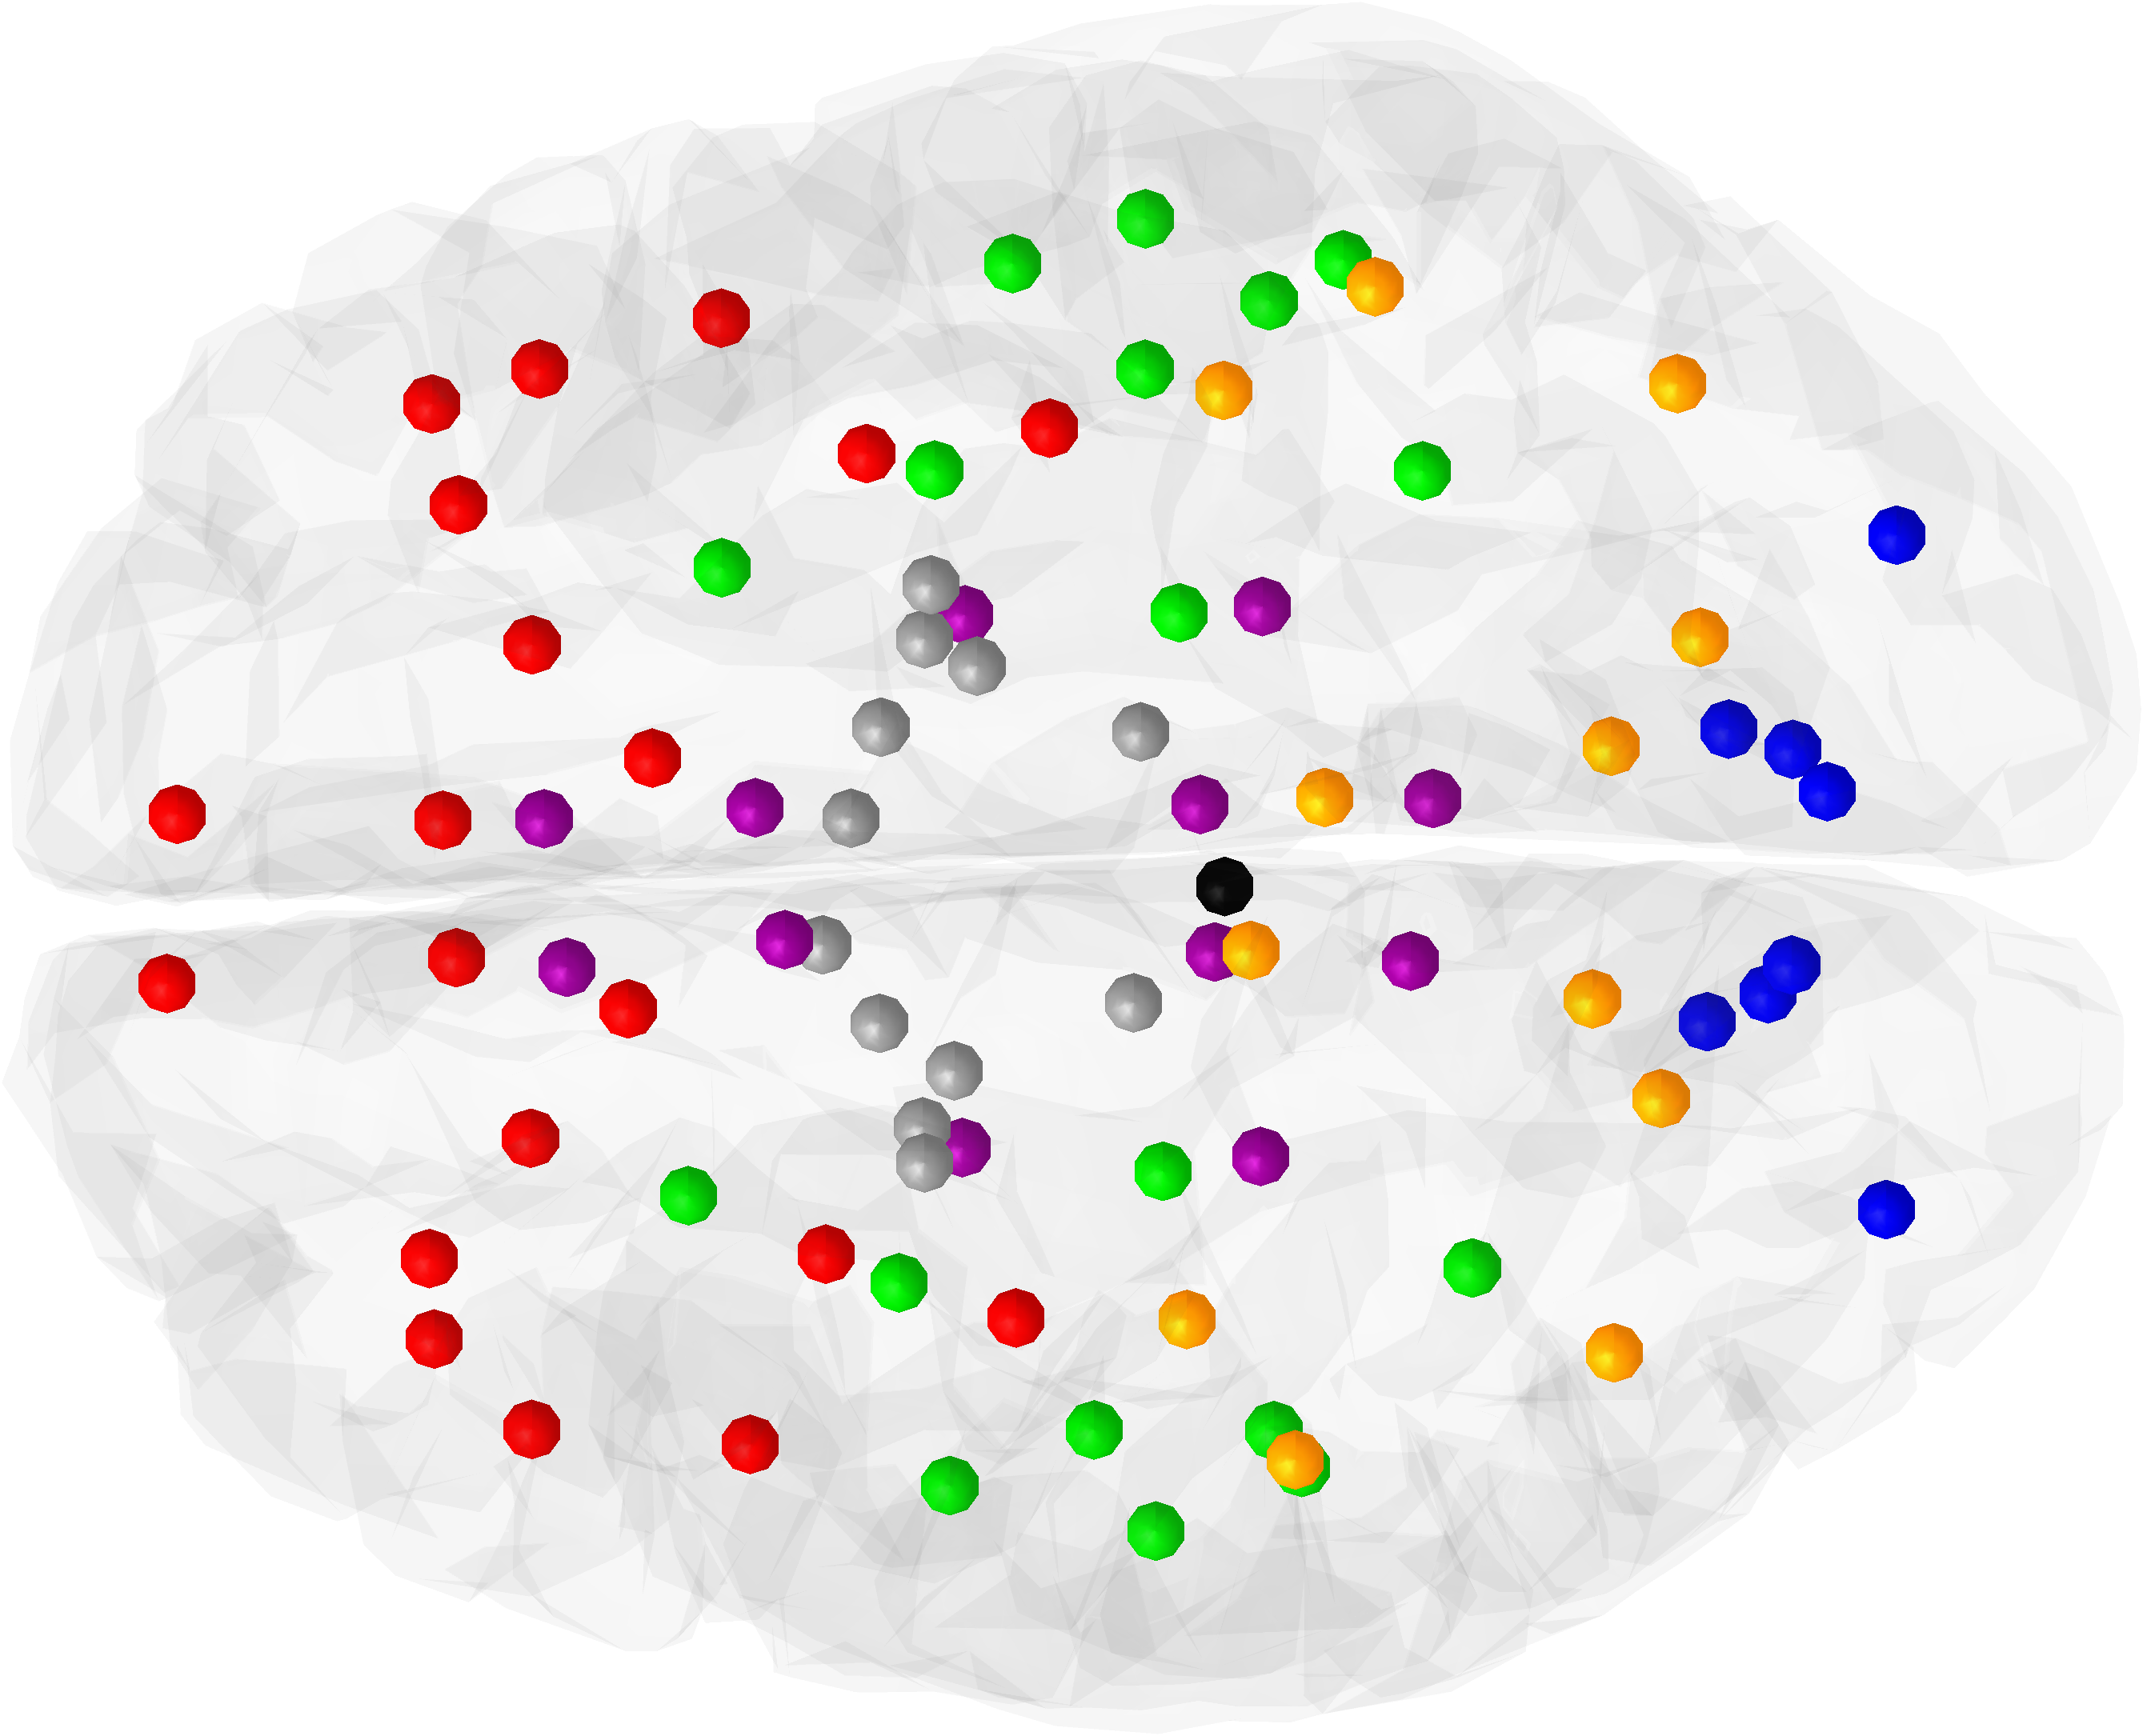
\includegraphics[width=\widthIm cm]{../Figure/regioniCervelloAlto [Trasparente].png}};
    \node[anchor=north west] at (FKHD c2r2.north west)
        {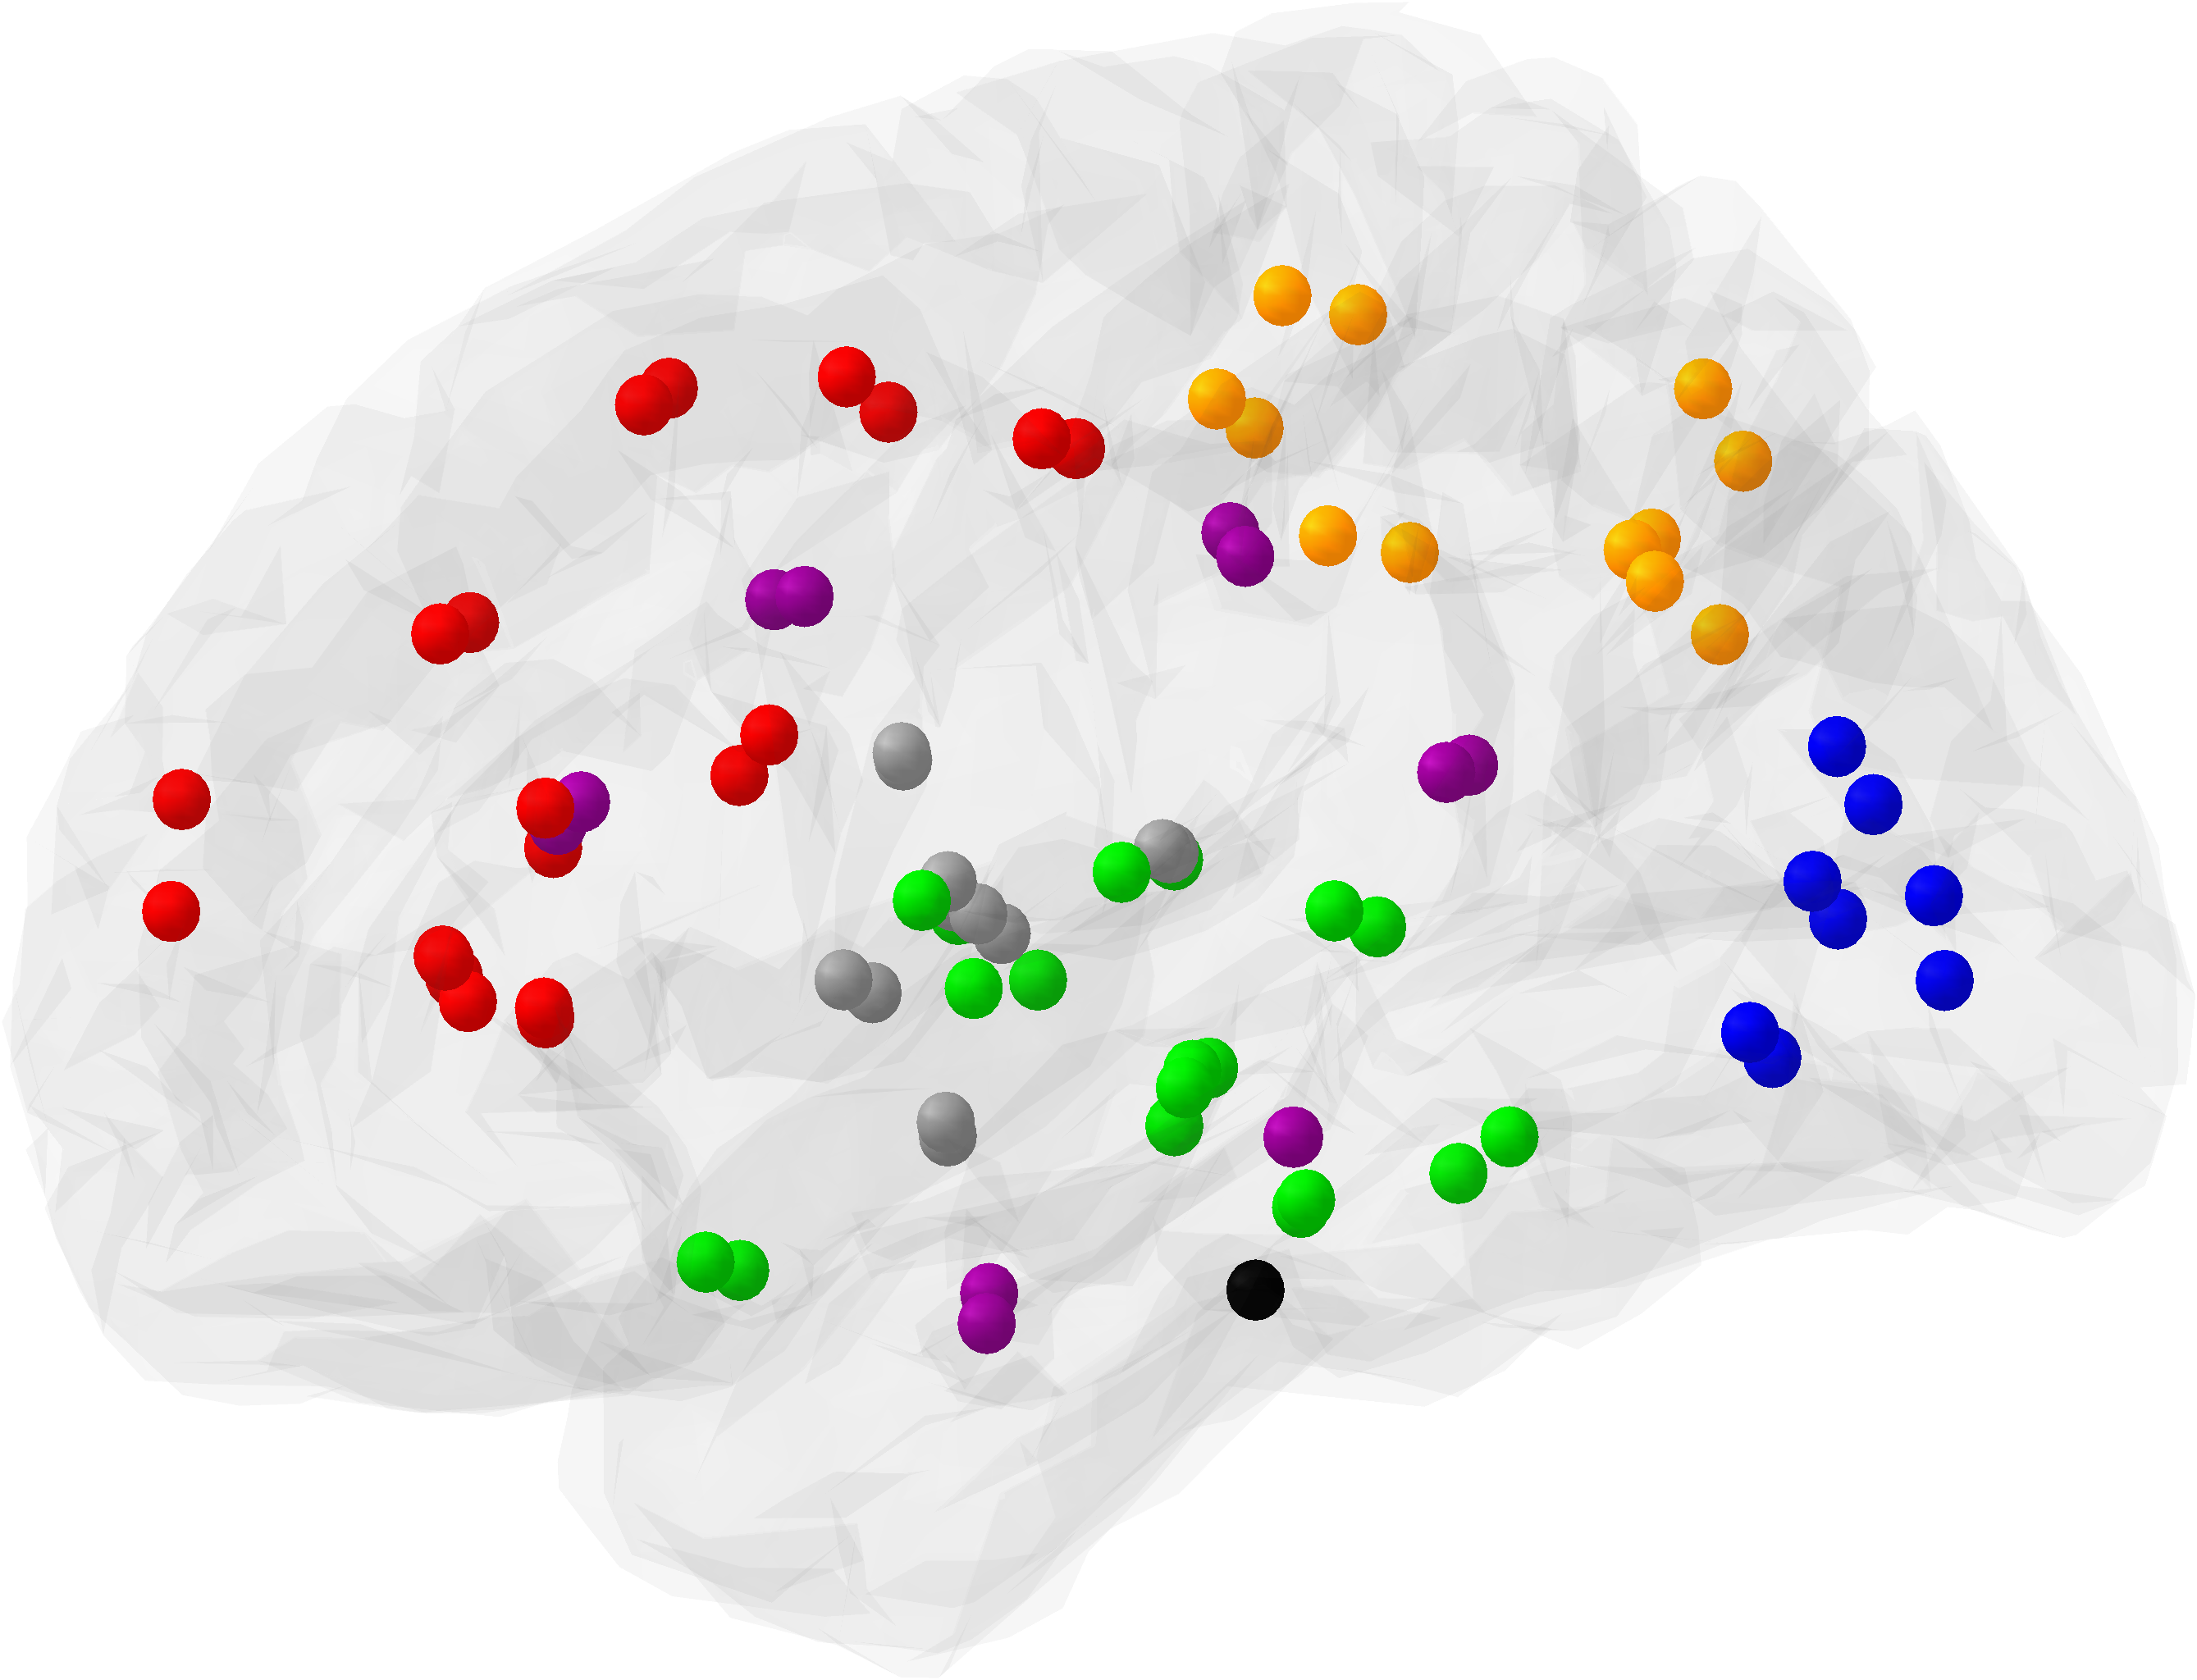
\includegraphics[width=\widthIm cm]{../Figure/regioniCervelloLato [Trasparente].png}};
    \newlength\heightIm
    \settoheight{\heightIm}{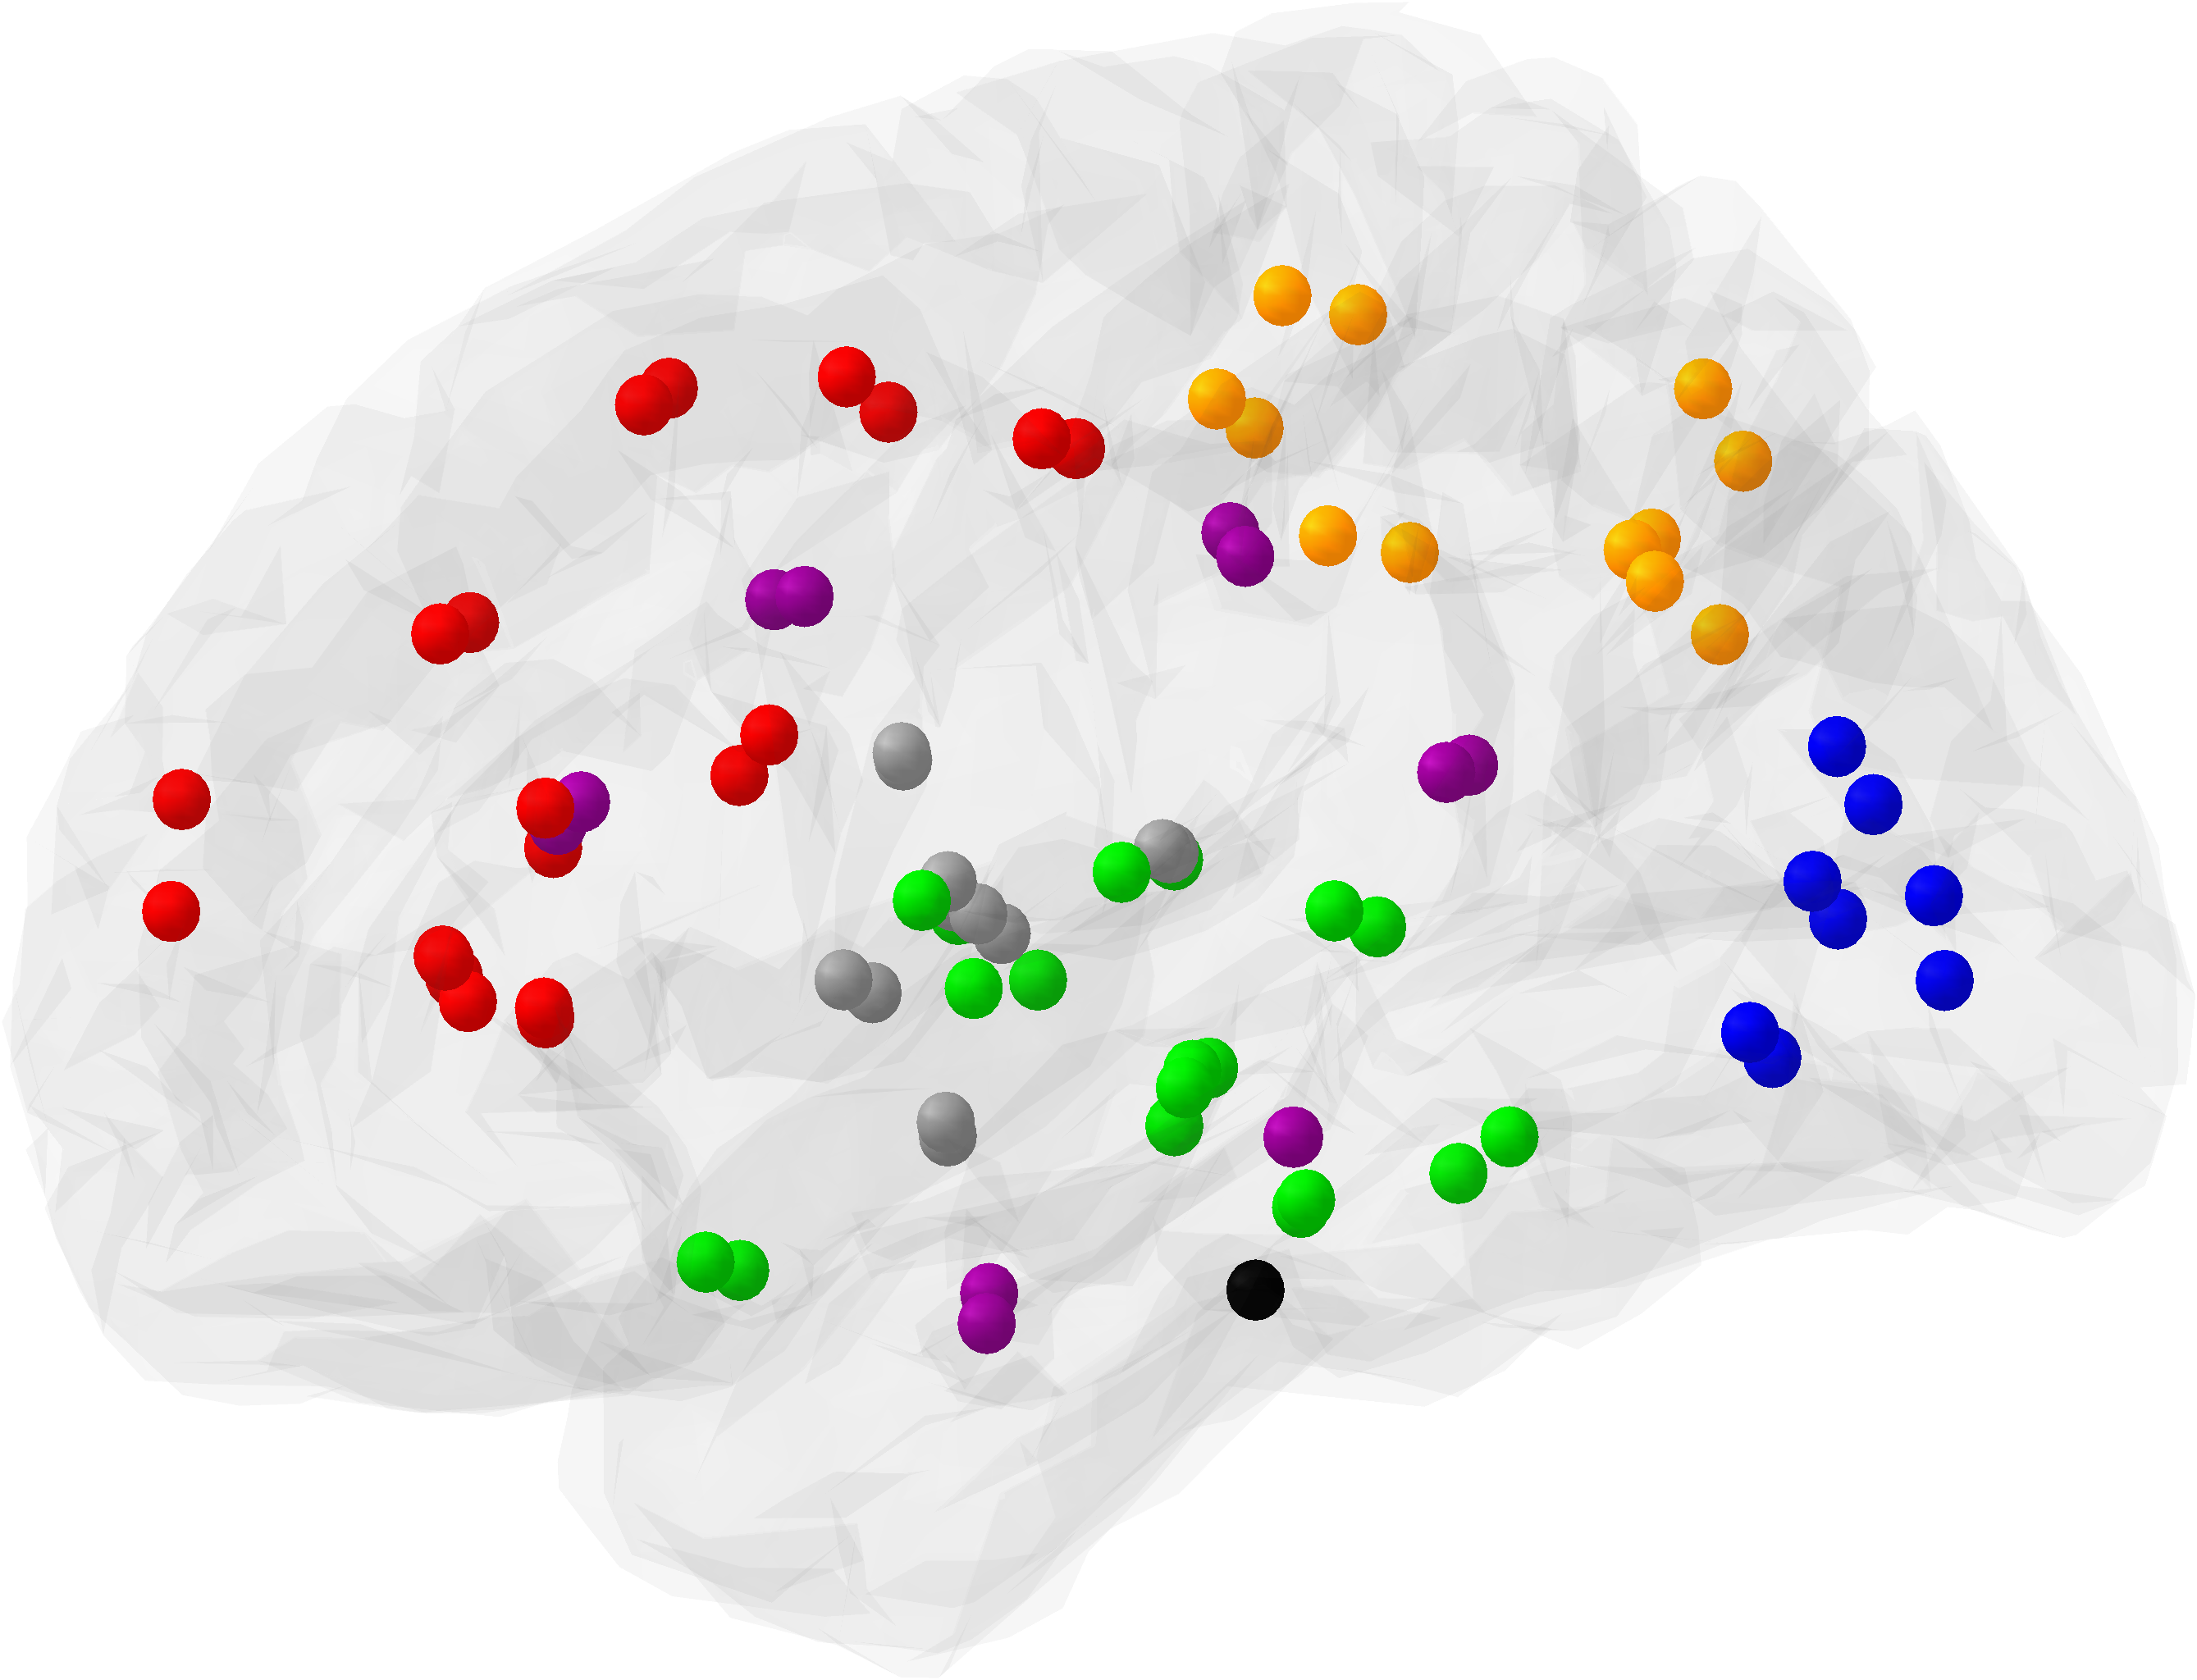
\includegraphics[width=\widthIm cm]{../Figure/regioniCervelloLato [Trasparente].png}}
    \node[anchor=north west] at (FKHD c1r2.north west)
        {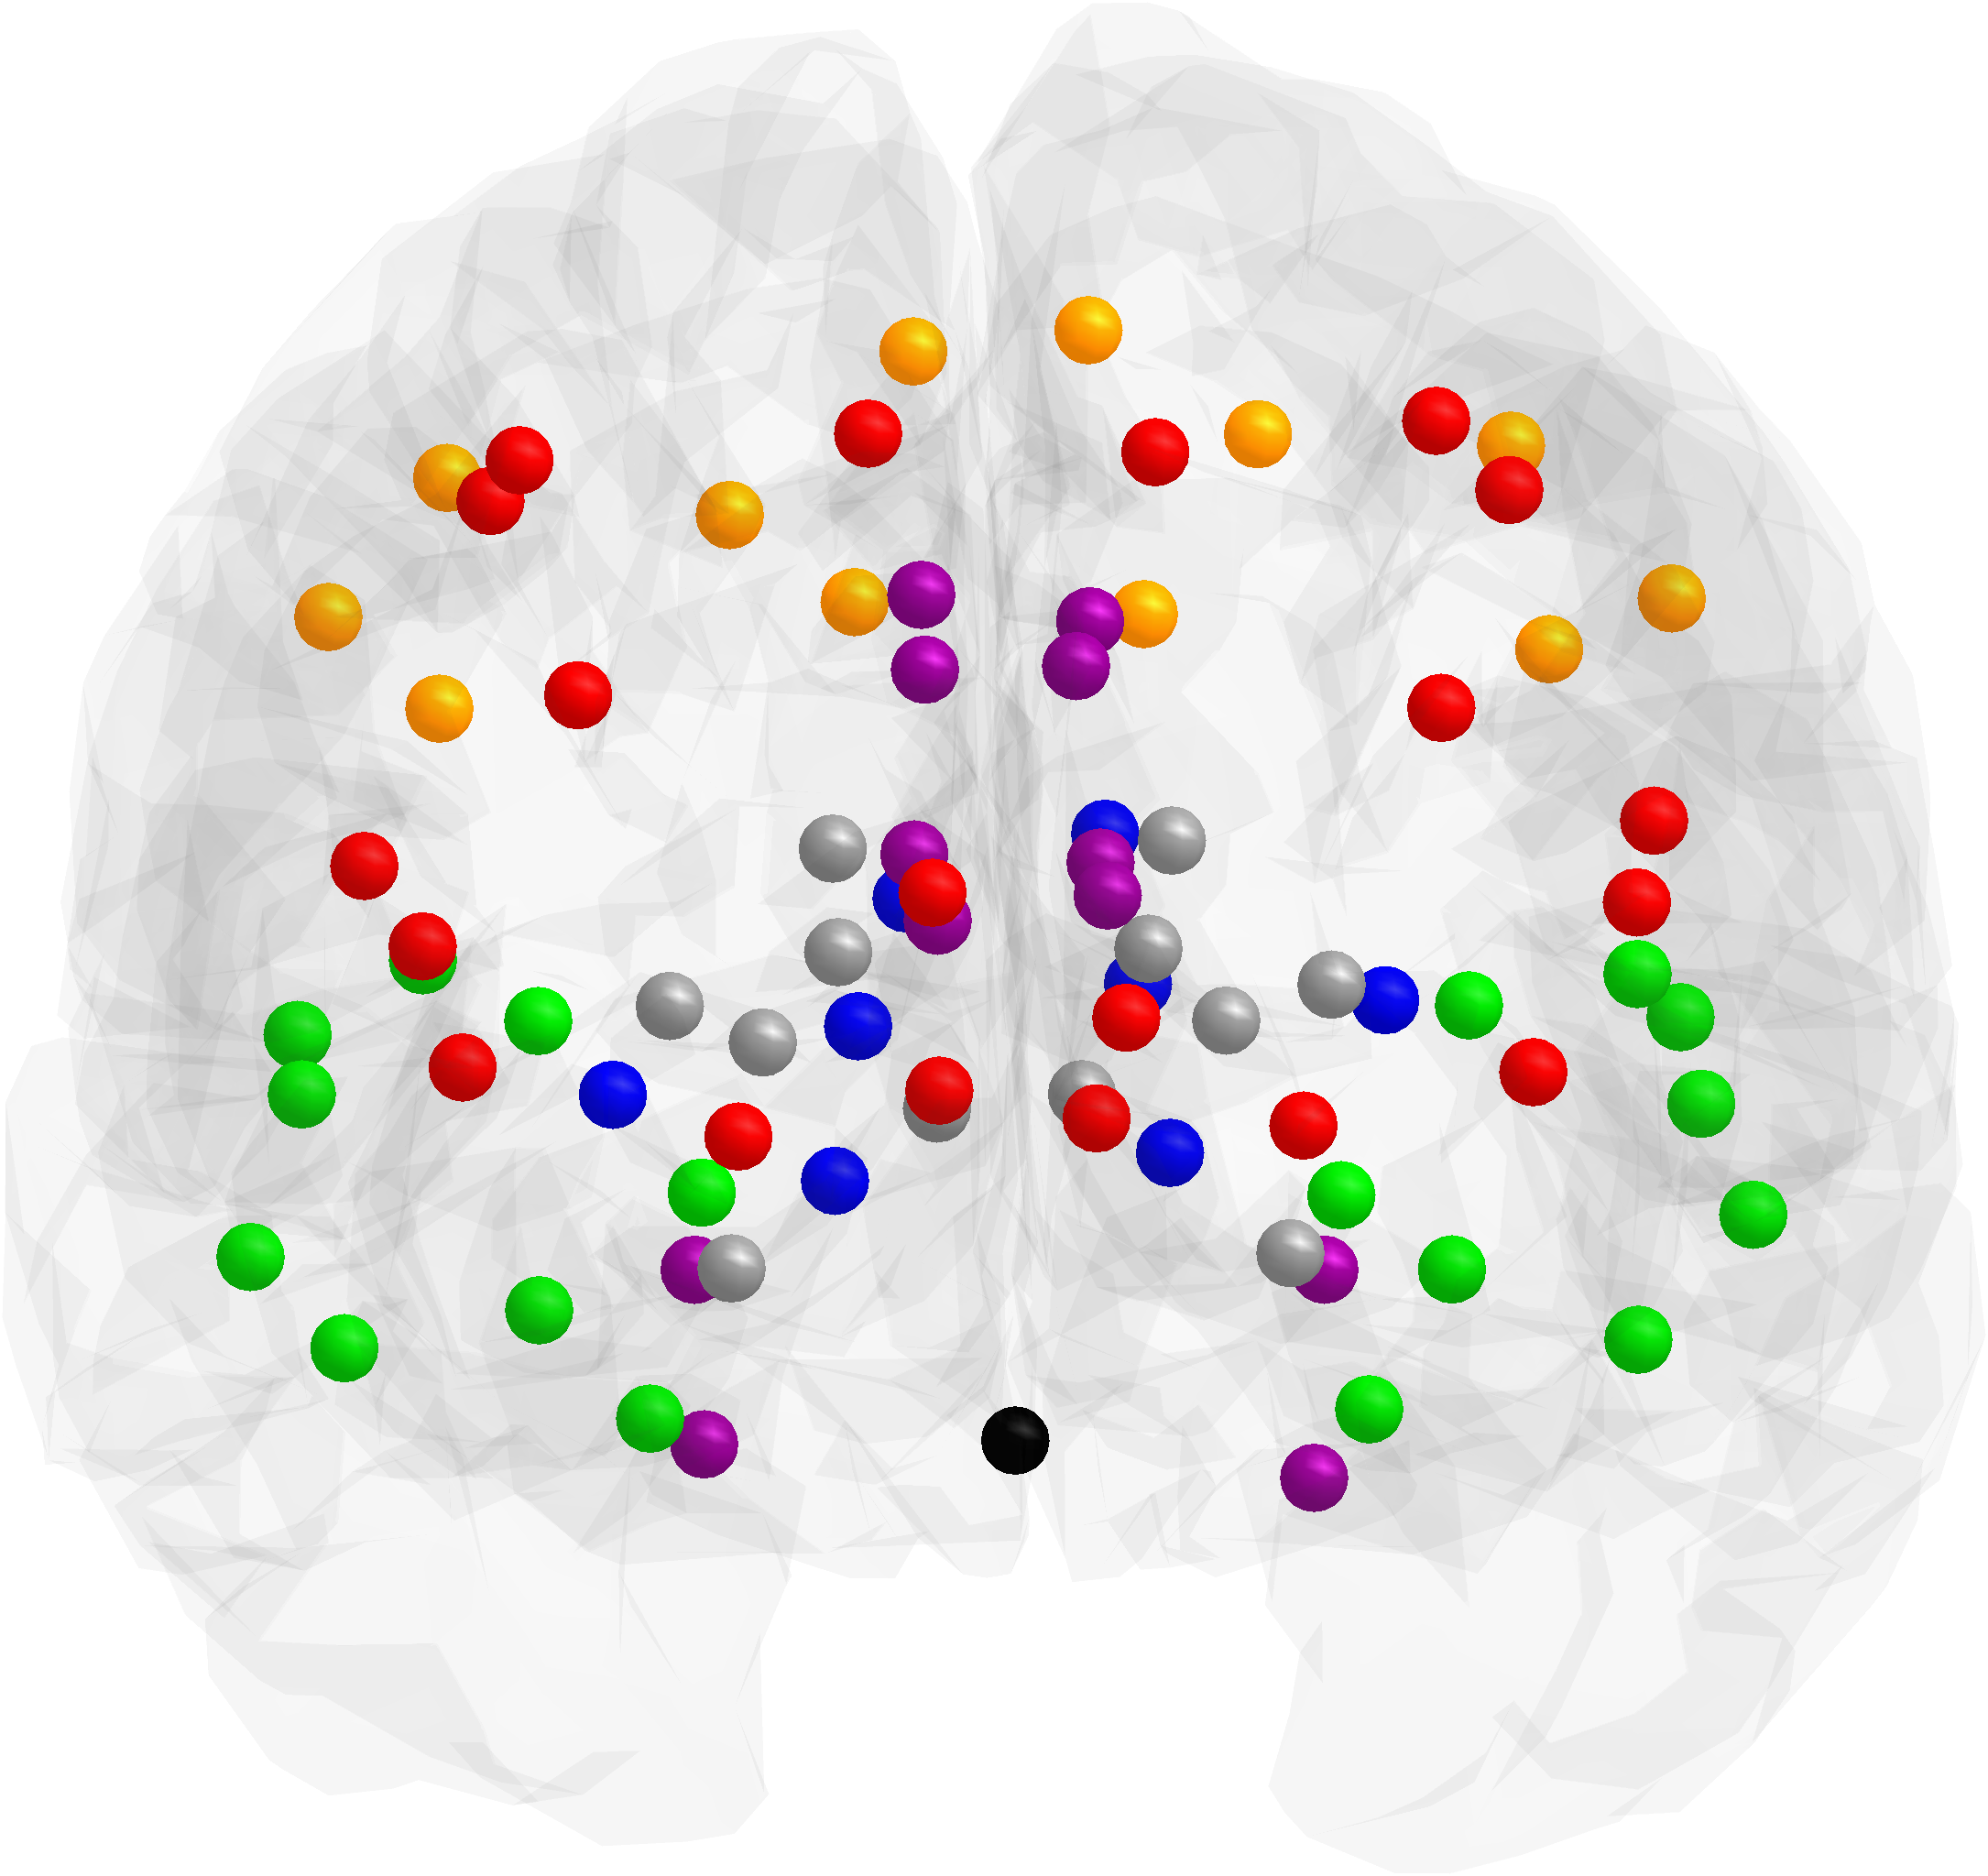
\includegraphics[height=\heightIm]{../Figure/regioniCervelloFronte [Trasparente].png}};

    \tikzset{SubCaption/.style={text width=14mm,anchor=south east,align=right}}
    \node[SubCaption] at (FKHD c1r1.south east) {\subcaption{FKS\label{figFKStaticL}}};
    \node[SubCaption] at (FKHD c1r2.south east) {\subcaption{FKD\label{figFKDynamicL}}};
    \node[SubCaption] at (FKHD c1r3.south east) {\subcaption{FKV$_1$\label{figFKDynamicLVariant1}}};
    \node[SubCaption] at (FKHD c1r4.south east) {\subcaption{FKV$_2$\label{figFKDynamicLVariant2}}};

    \node[SubCaption] at (FKHD c2r1.south east) {\subcaption{HDS\label{figHDStaticL}}};
    \node[SubCaption] at (FKHD c2r2.south east) {\subcaption{HDD\label{figHDDynamicL}}};
    \node[SubCaption] at (FKHD c2r3.south east) {\subcaption{HDV$_1$\label{figHDDynamicLVariant1}}};
    \node[SubCaption] at (FKHD c2r4.south east) {\subcaption{HDV$_2$\label{figHDDynamicLVariant2}}};
    % https://tex.stackexchange.com/questions/632045/get-subcaption-for-every-plot-using-groupplot-pgf-tikz-after-2020-update

    % Alternativa per imporre i titoli alle singole colonne
    % \pgfmathsetmacro\titleShift{0.2}
    % \node[above,yshift=\titleShift cm,style={font=\bfseries\tSizeTitle}]
    %     at (FKHD c1r1.north) {\selezionaLingua{Modello \FKdiscrete{}}{\FKdiscrete{} model}};
    % \node[above,yshift=\titleShift cm,style={font=\bfseries\tSizeTitle}]
    %     at (FKHD c2r1.north) {\selezionaLingua{Modello \HDdiscrete{}}{\HDdiscrete{} model}};
\end{tikzpicture}%

    % \pgfmathsetmacro\widthBrain{0}
    % \pgfmathsetmacro\sepxBrain{0}
    % \pgfmathsetmacro\distancexBrain{\widthBrain+\sepxBrain}
    % \pgfmathsetmacro\heightBrain{10}
    % \pgfmathsetmacro\sepyBrain{\sepxBrain}
    % \pgfmathsetmacro\distanceyBrain{\heightBrain+\sepyBrain}

    % \pgfmathsetmacro\sepxCurves{1}
    % \pgfmathsetmacro\distancexCurves{\widthCurves+\sepxCurves}
    % \pgfmathsetmacro\sepyCurves{\sepxCurves}
    % \pgfmathsetmacro\distanceyCurves{\heightCurves+\sepyCurves}

    % \coordinate (FKS) at (0,\distanceyCurves cm);
    % \begin{axis}[%
    %             width=\widthCurves cm,% 10.45in
    %             height=\heightCurves cm,% height=6.328in,
    %             at={(FKS)},
    %             scale only axis,
    %             title style={font=\bfseries\tSizeTitle},
    %             title={\selezionaLingua{Modello \FKdiscrete}{\FKdiscrete model}},
    %             xmin=0,xmax=30,
    %             xlabel style={font=\color{white!15!black}\tSizeLabel,
    %                         at={(ticklabel cs:1.0)},
    %                         anchor=east,
    %                         yshift=-.3cm,
    %                         },
    %             xlabel={\selezionaLingua{Tempo [anni]}{Time [years]}},
    %             ymin=0,ymax=1,
    %             ylabel style={font=\color{white!15!black}\tSizeLabel,
    %                         at={(ticklabel cs:1.0)},
    %                         anchor=east,
    %                         yshift=.3cm,
    %                         },
    %             ylabel={\selezionaLingua{Concentrazione}{Concentration} [M]},
    %             axis background/.style={fill=white},
    %             axis x line*=bottom,
    %             axis y line*=left,
    %             xmajorgrids,
    %             ymajorgrids,
    %             grid style={dashed},
    %             legend style={legend cell align=left,
    %                         align=left,
    %                         legend pos=north west,
    %                         draw=white!15!black,
    %                         font=\tSizeLegend,
    %                         fill=none,
    %                         draw=none,
    %                         },
    %             ]
    %     \addplot [color=black,dashed,line width=\lineWidth]
    %     table[row sep=crcr]{%
    %     0	0.00240963855421687\\
    %     0.4	0.00292466694502703\\
    %     0.8	0.00353051798613887\\
    %     1.2	0.00423575301794363\\
    %     1.6	0.00504723498398421\\
    %     2	0.00596943575665791\\
    %     2.4	0.00700393571996942\\
    %     2.8	0.00814928980826412\\
    %     3.2	0.00940141280649278\\
    %     3.6	0.0107545683067739\\
    %     4	0.0122029430445444\\
    %     4.4	0.013742681545431\\
    %     4.8	0.0153741809372758\\
    %     5.2	0.0171044273808024\\
    %     5.6	0.018949196354367\\
    %     6	0.0209350192977247\\
    %     6.4	0.0231009077937727\\
    %     6.8	0.0254998949309883\\
    %     7.2	0.0282004848774382\\
    %     7.6	0.0312880926644489\\
    %     8	0.0348665130872544\\
    %     8.4	0.0390593910331643\\
    %     8.8	0.0440115859207532\\
    %     9.2	0.0498902386294065\\
    %     9.6	0.0568852662403863\\
    %     10	0.0652089321886856\\
    %     10.4	0.075094070495834\\
    %     10.8	0.0867904876309496\\
    %     11.2	0.100559034469464\\
    %     11.6	0.11666285391722\\
    %     12	0.135355400497225\\
    %     12.4	0.156865041896579\\
    %     12.8	0.181376436304854\\
    %     13.2	0.209009461484802\\
    %     13.6	0.239797230658633\\
    %     14	0.273665563845014\\
    %     14.4	0.31041699072444\\
    %     14.8	0.349722666287717\\
    %     15.2	0.391125208621918\\
    %     15.6	0.434054267035927\\
    %     16	0.477854688439047\\
    %     16.4	0.521824851858232\\
    %     16.8	0.565260681986777\\
    %     17.2	0.607499646098651\\
    %     17.6	0.647959070337275\\
    %     18	0.686164370106723\\
    %     18.4	0.721764866881444\\
    %     18.8	0.754537130166669\\
    %     19.2	0.78437764431403\\
    %     19.6	0.811287703588204\\
    %     20	0.835353742070593\\
    %     20.4	0.856725998021404\\
    %     20.8	0.875597777062596\\
    %     21.2	0.892186863129925\\
    %     21.6	0.906719983869656\\
    %     22	0.919420726659844\\
    %     22.4	0.93050092051795\\
    %     22.8	0.940155222610056\\
    %     23.2	0.948558453341951\\
    %     23.6	0.95586510062275\\
    %     24	0.962210360831135\\
    %     24.4	0.967712101522667\\
    %     24.8	0.972473212389165\\
    %     25.2	0.976583938997425\\
    %     25.6	0.980123942011573\\
    %     26	0.983163964488453\\
    %     26.4	0.985767099239845\\
    %     26.8	0.987989716732996\\
    %     27.2	0.989882143198024\\
    %     27.6	0.991489178331879\\
    %     28	0.992850524801953\\
    %     28.4	0.99400117867426\\
    %     28.8	0.994971808297807\\
    %     29.2	0.995789132675063\\
    %     29.6	0.996476299730123\\
    %     30	0.997053259343476\\
    %     };
    %     \addlegendentry{\selezionaLingua{Rete}{Network}}

    %     \addplot [color=mycolor3,line width=\lineWidth]
    %     table[row sep=crcr]{%
    %     0	0\\
    %     0.4	7.04171308035969e-05\\
    %     0.8	0.000167204870158116\\
    %     1.2	0.000297593640187517\\
    %     1.6	0.000470390013802762\\
    %     2	0.000696245355284452\\
    %     2.4	0.000987971062313396\\
    %     2.8	0.0013609184425676\\
    %     3.2	0.00183344759533764\\
    %     3.6	0.00242751517133566\\
    %     4	0.00316941440823425\\
    %     4.4	0.00409070162786215\\
    %     4.8	0.00522934121508573\\
    %     5.2	0.0066310960862461\\
    %     5.6	0.00835118270409855\\
    %     6	0.0104561978995399\\
    %     6.4	0.0130263069503896\\
    %     6.8	0.0161576549880046\\
    %     7.2	0.0199649221440306\\
    %     7.6	0.0245838816770031\\
    %     8	0.0301737350345202\\
    %     8.4	0.0369188864319309\\
    %     8.8	0.0450296858239076\\
    %     9.2	0.0547415269702302\\
    %     9.6	0.0663115655831689\\
    %     10	0.0800122689302961\\
    %     10.4	0.0961210876435003\\
    %     10.8	0.114905823369987\\
    %     11.2	0.136605802613272\\
    %     11.6	0.161409749715755\\
    %     12	0.189432177122903\\
    %     12.4	0.220690968896398\\
    %     12.8	0.255089347297504\\
    %     13.2	0.292405334190111\\
    %     13.6	0.332291046146569\\
    %     14	0.374282810572877\\
    %     14.4	0.41782147487804\\
    %     14.8	0.462280801851337\\
    %     15.2	0.507000837513125\\
    %     15.6	0.551322761370546\\
    %     16	0.594621937573151\\
    %     16.4	0.636336489355429\\
    %     16.8	0.675989495718517\\
    %     17.2	0.713203702148864\\
    %     17.6	0.747708388248447\\
    %     18	0.779338741331604\\
    %     18.4	0.808028728216808\\
    %     18.8	0.833798971667276\\
    %     19.2	0.856741436627096\\
    %     19.6	0.877002761951682\\
    %     20	0.894767852410365\\
    %     20.4	0.910244952626059\\
    %     20.8	0.923652965639442\\
    %     21.2	0.935211348638105\\
    %     21.6	0.945132577493601\\
    %     22	0.953616942421616\\
    %     22.4	0.960849312865438\\
    %     22.8	0.966997468289605\\
    %     23.2	0.972211606252418\\
    %     23.6	0.976624685770879\\
    %     24	0.980353324229183\\
    %     24.4	0.983499027729342\\
    %     24.8	0.986149590853921\\
    %     25.2	0.988380549116344\\
    %     25.6	0.990256605153449\\
    %     26	0.991832978589798\\
    %     26.4	0.993156650736144\\
    %     26.8	0.994267490329762\\
    %     27.2	0.995199256770219\\
    %     27.6	0.995980483956158\\
    %     28	0.996635251872164\\
    %     28.4	0.99718385528054\\
    %     28.8	0.997643379824385\\
    %     29.2	0.99802819597514\\
    %     29.6	0.998350380868111\\
    %     30	0.998620077379601\\
    %     };
    %     \addlegendentry{\selezionaLingua{Temporale}{Temporal}}

    %     \addplot [color=black!20!red,line width=\lineWidth]
    %     table[row sep=crcr]{%
    %     0	0\\
    %     0.4	7.45220646300966e-07\\
    %     0.8	2.66053818596208e-06\\
    %     1.2	6.33256066900085e-06\\
    %     1.6	1.25599498691129e-05\\
    %     2	2.241734705516e-05\\
    %     2.4	3.73363879315073e-05\\
    %     2.8	5.92082605309713e-05\\
    %     3.2	9.05135077117992e-05\\
    %     3.6	0.000134486352877924\\
    %     4	0.000195322780129857\\
    %     4.4	0.000278443973293889\\
    %     4.8	0.000390829557993454\\
    %     5.2	0.00054143844202212\\
    %     5.6	0.00074173894457773\\
    %     6	0.00100637433954359\\
    %     6.4	0.00135399482479097\\
    %     6.8	0.00180829203008187\\
    %     7.2	0.00239927699995421\\
    %     7.6	0.00316484624780853\\
    %     8	0.00415268148980439\\
    %     8.4	0.00542252468862328\\
    %     8.8	0.00704885754264415\\
    %     9.2	0.00912398850054974\\
    %     9.6	0.0117615039533301\\
    %     10	0.0150999649500393\\
    %     10.4	0.0193066172028648\\
    %     10.8	0.0245807221693847\\
    %     11.2	0.0311559081354826\\
    %     11.6	0.0393006929190065\\
    %     12	0.0493160776800665\\
    %     12.4	0.0615289222558616\\
    %     12.8	0.0762797949966692\\
    %     13.2	0.0939042850402617\\
    %     13.6	0.114707509671646\\
    %     14	0.138932808211116\\
    %     14.4	0.166727286533402\\
    %     14.8	0.19810862665779\\
    %     15.2	0.232938846193422\\
    %     15.6	0.270910855936081\\
    %     16	0.311552298421052\\
    %     16.4	0.354248315256106\\
    %     16.8	0.398281235288992\\
    %     17.2	0.442881758741721\\
    %     17.6	0.487284085239131\\
    %     18	0.530777186563423\\
    %     18.4	0.572745950289678\\
    %     18.8	0.612698521217241\\
    %     19.2	0.650278930263997\\
    %     19.6	0.685266305411508\\
    %     20	0.717563301993666\\
    %     20.4	0.747176945500301\\
    %     20.8	0.774195108169195\\
    %     21.2	0.798761585883031\\
    %     21.6	0.821052339376459\\
    %     22	0.841254948590856\\
    %     22.4	0.859552699222201\\
    %     22.8	0.876113995914675\\
    %     23.2	0.891087044727256\\
    %     23.6	0.904599073641675\\
    %     24	0.91675887415578\\
    %     24.4	0.927661227032313\\
    %     24.8	0.937391838417236\\
    %     25.2	0.946031708063282\\
    %     25.6	0.953660276502649\\
    %     26	0.960357132827813\\
    %     26.4	0.966202411348837\\
    %     26.8	0.971276213283063\\
    %     27.2	0.975657458642253\\
    %     27.6	0.979422538204629\\
    %     28	0.982644043067448\\
    %     28.4	0.985389741598484\\
    %     28.8	0.987721878330469\\
    %     29.2	0.989696799295266\\
    %     29.6	0.991364865235621\\
    %     30	0.992770593646708\\
    %     };
    %     \addlegendentry{\selezionaLingua{Frontale}{Frontal}}

    %     \addplot [color=mycolor1,line width=\lineWidth]
    %     table[row sep=crcr]{%
    %     0	0\\
    %     0.4	2.92265476511246e-06\\
    %     0.8	9.40518562876442e-06\\
    %     1.2	2.1104874934221e-05\\
    %     1.6	4.02366709361745e-05\\
    %     2	6.97272979877064e-05\\
    %     2.4	0.000113406548683649\\
    %     2.8	0.000176244567594473\\
    %     3.2	0.000264646276215875\\
    %     3.6	0.000386816955090104\\
    %     4	0.000553216384794846\\
    %     4.4	0.00077712280831913\\
    %     4.8	0.00107533222978494\\
    %     5.2	0.00146902306663324\\
    %     5.6	0.00198482067286371\\
    %     6	0.00265610029766132\\
    %     6.4	0.00352456984877898\\
    %     6.8	0.00464217408983256\\
    %     7.2	0.00607335757215882\\
    %     7.6	0.00789771164358039\\
    %     8	0.0102130069863918\\
    %     8.4	0.0131385715675173\\
    %     8.8	0.0168189074970212\\
    %     9.2	0.0214273411411894\\
    %     9.6	0.0271693617230503\\
    %     10	0.034285121216271\\
    %     10.4	0.0430503483346543\\
    %     10.8	0.0537746942084826\\
    %     11.2	0.0667963248251199\\
    %     11.6	0.0824714860410682\\
    %     12	0.101157903195292\\
    %     12.4	0.123191365209137\\
    %     12.8	0.148855779982265\\
    %     13.2	0.178348375906261\\
    %     13.6	0.211743397962046\\
    %     14	0.248959235885559\\
    %     14.4	0.289734896840568\\
    %     14.8	0.333621560856513\\
    %     15.2	0.379993320328902\\
    %     15.6	0.428078218720781\\
    %     16	0.477006975098947\\
    %     16.4	0.525873271922735\\
    %     16.8	0.573797192504654\\
    %     17.2	0.619982987431953\\
    %     17.6	0.663763898076259\\
    %     18	0.704629727625241\\
    %     18.4	0.742236302679383\\
    %     18.8	0.776398977177477\\
    %     19.2	0.807074272812733\\
    %     19.6	0.834334449765346\\
    %     20	0.858339462782932\\
    %     20.4	0.879309781315215\\
    %     20.8	0.897502351364318\\
    %     21.2	0.913190857610115\\
    %     21.6	0.926650572754294\\
    %     22	0.93814750224563\\
    %     22.4	0.94793121600546\\
    %     22.8	0.956230640131781\\
    %     23.2	0.963252092054869\\
    %     23.6	0.969178924592125\\
    %     24	0.974172256203463\\
    %     24.4	0.978372380181864\\
    %     24.8	0.981900550126303\\
    %     25.2	0.984860926612823\\
    %     25.6	0.987342539274895\\
    %     26	0.98942117097036\\
    %     26.4	0.99116110895274\\
    %     26.8	0.992616734850643\\
    %     27.2	0.993833943457759\\
    %     27.6	0.994851392113816\\
    %     28	0.995701589630964\\
    %     28.4	0.996411837687894\\
    %     28.8	0.997005039416993\\
    %     29.2	0.997500390303335\\
    %     29.6	0.99791396603275\\
    %     30	0.998259220939444\\
    %     };
    %     \addlegendentry{\selezionaLingua{Parietale}{Parietal}}

    %     \addplot [color=black!20!blue,line width=\lineWidth]
    %     table[row sep=crcr]{%
    %     0	0\\
    %     0.4	1.82060656035219e-06\\
    %     0.8	5.93546786074805e-06\\
    %     1.2	1.35351497142175e-05\\
    %     1.6	2.62564063765037e-05\\
    %     2	4.63198496736759e-05\\
    %     2.4	7.67048465576021e-05\\
    %     2.8	0.000121371193016582\\
    %     3.2	0.000185539621371945\\
    %     3.6	0.000276046287662828\\
    %     4	0.00040179009783212\\
    %     4.4	0.00057429607811972\\
    %     4.8	0.000808422946490247\\
    %     5.2	0.00112324849503181\\
    %     5.6	0.00154317211057589\\
    %     6	0.00209927926737817\\
    %     6.4	0.00283101725450338\\
    %     6.8	0.00378823327742031\\
    %     7.2	0.00503362303461754\\
    %     7.6	0.00664562631835361\\
    %     8	0.00872178092272865\\
    %     8.4	0.0113825000627665\\
    %     8.8	0.0147751626203496\\
    %     9.2	0.019078289644927\\
    %     9.6	0.0245054152992387\\
    %     10	0.0313080415767264\\
    %     10.4	0.0397768016856432\\
    %     10.8	0.0502396778242263\\
    %     11.2	0.0630558905818281\\
    %     11.6	0.0786040071999099\\
    %     12	0.0972630483996104\\
    %     12.4	0.119386055925335\\
    %     12.8	0.145266799818201\\
    %     13.2	0.175101987892219\\
    %     13.6	0.208953196818254\\
    %     14	0.246714259974159\\
    %     14.4	0.288090411383867\\
    %     14.8	0.332594625073826\\
    %     15.2	0.379564217670446\\
    %     15.6	0.428197327020663\\
    %     16	0.477605201204776\\
    %     16.4	0.526873332871975\\
    %     16.8	0.575123121280996\\
    %     17.2	0.621566192579499\\
    %     17.6	0.665545454650225\\
    %     18	0.706559740243492\\
    %     18.4	0.744271758454113\\
    %     18.8	0.778501438923011\\
    %     19.2	0.809208277325879\\
    %     19.6	0.836466892850385\\
    %     20	0.860439811808843\\
    %     20.4	0.881350747549608\\
    %     20.8	0.899460645938441\\
    %     21.2	0.915047760765474\\
    %     21.6	0.928392183109885\\
    %     22	0.93976464855263\\
    %     22.4	0.949419087564854\\
    %     22.8	0.957588224803374\\
    %     23.2	0.9644815136983\\
    %     23.6	0.97028475762078\\
    %     24	0.975160874011668\\
    %     24.4	0.979251373183774\\
    %     24.8	0.982678231460473\\
    %     25.2	0.985545930404855\\
    %     25.6	0.987943507575933\\
    %     26	0.989946520350978\\
    %     26.4	0.991618865306762\\
    %     26.8	0.993014424388812\\
    %     27.2	0.994178528446192\\
    %     27.6	0.995149241116129\\
    %     28	0.995958473487697\\
    %     28.4	0.996632943983268\\
    %     28.8	0.997194999607051\\
    %     29.2	0.997663314942787\\
    %     29.6	0.99805348461454\\
    %     30	0.998378523751173\\
    %     };
    %     \addlegendentry{\selezionaLingua{Occipitale}{Occipital}}

    %     \addplot [color=mycolor2,line width=\lineWidth]
    %     table[row sep=crcr]{%
    %     0	0.0166666666666667\\
    %     0.4	0.0200992326918299\\
    %     0.8	0.0241027202126695\\
    %     1.2	0.0287184684026006\\
    %     1.6	0.0339715450849803\\
    %     2	0.0398649948263615\\
    %     2.4	0.0463752166314689\\
    %     2.8	0.0534496166861802\\
    %     3.2	0.0610075150679463\\
    %     3.6	0.0689447932395919\\
    %     4	0.0771420416528467\\
    %     4.4	0.0854752137947074\\
    %     4.8	0.0938272629742382\\
    %     5.2	0.102099103874781\\
    %     5.6	0.110218520470747\\
    %     6	0.118146201696556\\
    %     6.4	0.125878716821024\\
    %     6.8	0.133448755101637\\
    %     7.2	0.140923245352997\\
    %     7.6	0.148400033961324\\
    %     8	0.156003697567484\\
    %     8.4	0.163880891080927\\
    %     8.8	0.172195469932957\\
    %     9.2	0.181123538472244\\
    %     9.6	0.190848587099173\\
    %     10	0.201556967076065\\
    %     10.4	0.213434045793719\\
    %     10.8	0.226661384727149\\
    %     11.2	0.241415085731449\\
    %     11.6	0.257865011182176\\
    %     12	0.276173960662669\\
    %     12.4	0.296495272771936\\
    %     12.8	0.318966999628359\\
    %     13.2	0.343701054291667\\
    %     13.6	0.370766709517829\\
    %     14	0.400169449881374\\
    %     14.4	0.431828097941301\\
    %     14.8	0.465554780716429\\
    %     15.2	0.501043039477444\\
    %     15.6	0.537868735248558\\
    %     16	0.575506276359213\\
    %     16.4	0.613359527368757\\
    %     16.8	0.650803433456102\\
    %     17.2	0.687229941402174\\
    %     17.6	0.722090985214337\\
    %     18	0.754932316317563\\
    %     18.4	0.785414343888123\\
    %     18.8	0.813319057210153\\
    %     19.2	0.838544656331837\\
    %     19.6	0.861091148224767\\
    %     20	0.88104072514078\\
    %     20.4	0.898536426744558\\
    %     20.8	0.913761759229566\\
    %     21.2	0.926922958869747\\
    %     21.6	0.938234695975606\\
    %     22	0.947909343445865\\
    %     22.4	0.956149506685048\\
    %     22.8	0.963143293819441\\
    %     23.2	0.969061739133736\\
    %     23.6	0.974057821077516\\
    %     24	0.978266593257419\\
    %     24.4	0.981806041001591\\
    %     24.8	0.984778368415837\\
    %     25.2	0.9872715017291\\
    %     25.6	0.989360660627582\\
    %     26	0.991109900202996\\
    %     26.4	0.99257356383777\\
    %     26.8	0.993797614199399\\
    %     27.2	0.994820827923581\\
    %     27.6	0.99567585165889\\
    %     28	0.996390124672075\\
    %     28.4	0.996986677539259\\
    %     28.8	0.997484818597548\\
    %     29.2	0.997900720553733\\
    %     29.6	0.99824791947219\\
    %     30	0.998537737660785\\
    %     };
    %     \addlegendentry{\selezionaLingua{Limbico}{Limbic}}

    %     \addplot [color=mycolor4,line width=\lineWidth]
    %     table[row sep=crcr]{%
    %     0	0\\
    %     0.4	1.85701263021203e-05\\
    %     0.8	4.7583937669899e-05\\
    %     1.2	9.04937342308993e-05\\
    %     1.6	0.00015164402782878\\
    %     2	0.000236459234873285\\
    %     2.4	0.000351666710831065\\
    %     2.8	0.000505563925257762\\
    %     3.2	0.000708341314593663\\
    %     3.6	0.000972475203934879\\
    %     4	0.00131320781815544\\
    %     4.4	0.0017491334949915\\
    %     4.8	0.00230291154020361\\
    %     5.2	0.00300212656224813\\
    %     5.6	0.00388031638403485\\
    %     6	0.0049781853658182\\
    %     6.4	0.00634501650836823\\
    %     6.8	0.00804028803642506\\
    %     7.2	0.0101354880207717\\
    %     7.6	0.0127161026007343\\
    %     8	0.0158837282397216\\
    %     8.4	0.0197582252528462\\
    %     8.8	0.0244797881655102\\
    %     9.2	0.0302107583053129\\
    %     9.6	0.0371369453574326\\
    %     10	0.0454681564729742\\
    %     10.4	0.0554375513868799\\
    %     10.8	0.0672993468181004\\
    %     11.2	0.0813242845410382\\
    %     11.6	0.0977921712639161\\
    %     12	0.116980740658439\\
    %     12.4	0.139150164672244\\
    %     12.8	0.16452287196807\\
    %     13.2	0.193259029886559\\
    %     13.6	0.225429148854302\\
    %     14	0.260986649555533\\
    %     14.4	0.299744559541911\\
    %     14.8	0.341361276644008\\
    %     15.2	0.385340042393625\\
    %     15.6	0.431045127854367\\
    %     16	0.477734904529683\\
    %     16.4	0.524608605341166\\
    %     16.8	0.570860641887136\\
    %     17.2	0.615734750598733\\
    %     17.6	0.658570477182169\\
    %     18	0.698836431073164\\
    %     18.4	0.736147665786536\\
    %     18.8	0.770267559821757\\
    %     19.2	0.801096918829901\\
    %     19.6	0.828654296477781\\
    %     20	0.853051743646\\
    %     20.4	0.87446962311347\\
    %     20.8	0.893133147365423\\
    %     21.2	0.909292243234683\\
    %     21.6	0.923205437301385\\
    %     22	0.935127788709282\\
    %     22.4	0.945302479993981\\
    %     22.8	0.953955470070189\\
    %     23.2	0.961292557168762\\
    %     23.6	0.967498236250402\\
    %     24	0.972735820111998\\
    %     24.4	0.977148394953567\\
    %     24.8	0.980860280650155\\
    %     25.2	0.983978753638613\\
    %     25.6	0.986595862420315\\
    %     26	0.988790222051887\\
    %     26.4	0.990628716290233\\
    %     26.8	0.992168066651958\\
    %     27.2	0.993456248997251\\
    %     27.6	0.994533752571464\\
    %     28	0.995434685593531\\
    %     28.4	0.996187736946919\\
    %     28.8	0.996817006436351\\
    %     29.2	0.997342717264563\\
    %     29.6	0.997781824464797\\
    %     30	0.998148532427422\\
    %     };
    %     \addlegendentry{\selezionaLingua{Ganglia basale}{Basal ganglia}}

    %     \addplot [color=black,line width=\lineWidth]
    %     table[row sep=crcr]{%
    %     0	0\\
    %     0.4	1.67314260489751e-06\\
    %     0.8	6.09864845697023e-06\\
    %     1.2	1.50784136640462e-05\\
    %     1.6	3.11237689017431e-05\\
    %     2	5.76693583240359e-05\\
    %     2.4	9.93404129266404e-05\\
    %     2.8	0.000162285216564158\\
    %     3.2	0.000254587192541944\\
    %     3.6	0.000386774235926291\\
    %     4	0.000572446694154103\\
    %     4.4	0.000829049702201999\\
    %     4.8	0.00117882025983877\\
    %     5.2	0.00164994420952352\\
    %     5.6	0.00227796263077843\\
    %     6	0.00310747026910931\\
    %     6.4	0.00419414910622058\\
    %     6.8	0.00560717593221266\\
    %     7.2	0.00743203060766446\\
    %     7.6	0.00977370699253514\\
    %     8	0.012760284919661\\
    %     8.4	0.0165467508877955\\
    %     8.8	0.0213188476306358\\
    %     9.2	0.0272965785812348\\
    %     9.6	0.0347367858386367\\
    %     10	0.0439339621172544\\
    %     10.4	0.0552181698457438\\
    %     10.8	0.0689486776827674\\
    %     11.2	0.0855017853910897\\
    %     11.6	0.105251442420307\\
    %     12	0.128541858062425\\
    %     12.4	0.155652512921203\\
    %     12.8	0.186757844524447\\
    %     13.2	0.221886162859706\\
    %     13.6	0.260884470039204\\
    %     14	0.303396940939208\\
    %     14.4	0.348864008699504\\
    %     14.8	0.396545916206659\\
    %     15.2	0.445569748751284\\
    %     15.6	0.494993742540729\\
    %     16	0.543878814210849\\
    %     16.4	0.591356072145686\\
    %     16.8	0.63668079176671\\
    %     17.2	0.679267118843734\\
    %     17.6	0.718702181864157\\
    %     18	0.754742021481116\\
    %     18.4	0.787294021582292\\
    %     18.8	0.816391247581\\
    %     19.2	0.842163619196125\\
    %     19.6	0.864809698042677\\
    %     20	0.884571535292027\\
    %     20.4	0.901713824025692\\
    %     20.8	0.916507688282375\\
    %     21.2	0.929218843938952\\
    %     21.6	0.940099541512987\\
    %     22	0.949383576130526\\
    %     22.4	0.957283654235198\\
    %     22.8	0.963990482444332\\
    %     23.2	0.969673050418444\\
    %     23.6	0.974479690972158\\
    %     24	0.978539602775448\\
    %     24.4	0.981964607492476\\
    %     24.8	0.984850982594029\\
    %     25.2	0.987281264421187\\
    %     25.6	0.98932595566447\\
    %     26	0.991045099858214\\
    %     26.4	0.992489705256797\\
    %     26.8	0.993703013707172\\
    %     27.2	0.994721618614383\\
    %     27.6	0.995576441183431\\
    %     28	0.996293576853752\\
    %     28.4	0.996895024989219\\
    %     28.8	0.997399315002532\\
    %     29.2	0.997822041570551\\
    %     29.6	0.998176320708591\\
    %     30	0.998473177400279\\
    %     };
    %     \addlegendentry{\selezionaLingua{Tronco encefalico}{Brainstem}}

    % \end{axis}

    % \coordinate (FKD) at (0,0);
    % \begin{axis}[%
    %             width=\widthCurves cm,% 10.45in
    %             height=\heightCurves cm,% height=6.328in,
    %             at={(FKD)},
    %             scale only axis,
    %             title style={font=\bfseries\tSizeTitle},
    %             title={\selezionaLingua{Modello \FKdiscrete}{\FKdiscrete model}},
    %             xmin=0,xmax=30,
    %             xlabel style={font=\color{white!15!black}\tSizeLabel,
    %                         at={(ticklabel cs:1.0)},
    %                         anchor=east,
    %                         yshift=-.3cm,
    %                         },
    %             xlabel={\selezionaLingua{Tempo [anni]}{Time [years]}},
    %             ymin=0,ymax=1,
    %             ylabel style={font=\color{white!15!black}\tSizeLabel,
    %                         at={(ticklabel cs:1.0)},
    %                         anchor=east,
    %                         yshift=.3cm,
    %                         },
    %             ylabel={\selezionaLingua{Concentrazione}{Concentration} [M]},
    %             axis background/.style={fill=white},
    %             axis x line*=bottom,
    %             axis y line*=left,
    %             xmajorgrids,
    %             ymajorgrids,
    %             grid style={dashed},
    %             legend style={legend cell align=left,
    %                         align=left,
    %                         legend pos=north west,
    %                         draw=white!15!black,
    %                         font=\tSizeLegend,
    %                         fill=none,
    %                         draw=none,
    %                         },
    %             ]
    %     \addplot [color=black,dashed,line width=\lineWidth]
    %     table[row sep=crcr]{%
    %     0	0.00240963855421687\\
    %     0.4	0.00292466694502703\\
    %     0.8	0.00353051798613887\\
    %     1.2	0.00423575301794363\\
    %     1.6	0.00504723498398421\\
    %     2	0.00596943575665791\\
    %     2.4	0.00700393571996942\\
    %     2.8	0.00814928980826412\\
    %     3.2	0.00940141280649278\\
    %     3.6	0.0107545683067739\\
    %     4	0.0122029430445444\\
    %     4.4	0.013742681545431\\
    %     4.8	0.0153741809372758\\
    %     5.2	0.0171044273808024\\
    %     5.6	0.018949196354367\\
    %     6	0.0209350192977247\\
    %     6.4	0.0231009077937727\\
    %     6.8	0.0254998949309883\\
    %     7.2	0.0282004848774382\\
    %     7.6	0.0312880926644489\\
    %     8	0.0348665130872544\\
    %     8.4	0.0390593910331643\\
    %     8.8	0.0440115859207532\\
    %     9.2	0.0498902386294065\\
    %     9.6	0.0568852662403863\\
    %     10	0.0652089321886856\\
    %     10.4	0.075094070495834\\
    %     10.8	0.0867904876309496\\
    %     11.2	0.100559034469464\\
    %     11.6	0.11666285391722\\
    %     12	0.135355400497225\\
    %     12.4	0.156865041896579\\
    %     12.8	0.181376436304854\\
    %     13.2	0.209009461484802\\
    %     13.6	0.239797230658633\\
    %     14	0.273665563845014\\
    %     14.4	0.31041699072444\\
    %     14.8	0.349722666287717\\
    %     15.2	0.391125208621918\\
    %     15.6	0.434054267035927\\
    %     16	0.477854688439047\\
    %     16.4	0.521824851858232\\
    %     16.8	0.565260681986777\\
    %     17.2	0.607499646098651\\
    %     17.6	0.647959070337275\\
    %     18	0.686164370106723\\
    %     18.4	0.721764866881444\\
    %     18.8	0.754537130166669\\
    %     19.2	0.78437764431403\\
    %     19.6	0.811287703588204\\
    %     20	0.835353742070593\\
    %     20.4	0.856725998021404\\
    %     20.8	0.875597777062596\\
    %     21.2	0.892186863129925\\
    %     21.6	0.906719983869656\\
    %     22	0.919420726659844\\
    %     22.4	0.93050092051795\\
    %     22.8	0.940155222610056\\
    %     23.2	0.948558453341951\\
    %     23.6	0.95586510062275\\
    %     24	0.962210360831135\\
    %     24.4	0.967712101522667\\
    %     24.8	0.972473212389165\\
    %     25.2	0.976583938997425\\
    %     25.6	0.980123942011573\\
    %     26	0.983163964488453\\
    %     26.4	0.985767099239845\\
    %     26.8	0.987989716732996\\
    %     27.2	0.989882143198024\\
    %     27.6	0.991489178331879\\
    %     28	0.992850524801953\\
    %     28.4	0.99400117867426\\
    %     28.8	0.994971808297807\\
    %     29.2	0.995789132675063\\
    %     29.6	0.996476299730123\\
    %     30	0.997053259343476\\
    %     };
    %     \addlegendentry{\selezionaLingua{Rete}{Network}}

    %     \addplot [color=mycolor3,line width=\lineWidth]
    %     table[row sep=crcr]{%
    %     0	0\\
    %     0.4	7.04171308035969e-05\\
    %     0.8	0.000167204870158116\\
    %     1.2	0.000297593640187517\\
    %     1.6	0.000470390013802762\\
    %     2	0.000696245355284452\\
    %     2.4	0.000987971062313396\\
    %     2.8	0.0013609184425676\\
    %     3.2	0.00183344759533764\\
    %     3.6	0.00242751517133566\\
    %     4	0.00316941440823425\\
    %     4.4	0.00409070162786215\\
    %     4.8	0.00522934121508573\\
    %     5.2	0.0066310960862461\\
    %     5.6	0.00835118270409855\\
    %     6	0.0104561978995399\\
    %     6.4	0.0130263069503896\\
    %     6.8	0.0161576549880046\\
    %     7.2	0.0199649221440306\\
    %     7.6	0.0245838816770031\\
    %     8	0.0301737350345202\\
    %     8.4	0.0369188864319309\\
    %     8.8	0.0450296858239076\\
    %     9.2	0.0547415269702302\\
    %     9.6	0.0663115655831689\\
    %     10	0.0800122689302961\\
    %     10.4	0.0961210876435003\\
    %     10.8	0.114905823369987\\
    %     11.2	0.136605802613272\\
    %     11.6	0.161409749715755\\
    %     12	0.189432177122903\\
    %     12.4	0.220690968896398\\
    %     12.8	0.255089347297504\\
    %     13.2	0.292405334190111\\
    %     13.6	0.332291046146569\\
    %     14	0.374282810572877\\
    %     14.4	0.41782147487804\\
    %     14.8	0.462280801851337\\
    %     15.2	0.507000837513125\\
    %     15.6	0.551322761370546\\
    %     16	0.594621937573151\\
    %     16.4	0.636336489355429\\
    %     16.8	0.675989495718517\\
    %     17.2	0.713203702148864\\
    %     17.6	0.747708388248447\\
    %     18	0.779338741331604\\
    %     18.4	0.808028728216808\\
    %     18.8	0.833798971667276\\
    %     19.2	0.856741436627096\\
    %     19.6	0.877002761951682\\
    %     20	0.894767852410365\\
    %     20.4	0.910244952626059\\
    %     20.8	0.923652965639442\\
    %     21.2	0.935211348638105\\
    %     21.6	0.945132577493601\\
    %     22	0.953616942421616\\
    %     22.4	0.960849312865438\\
    %     22.8	0.966997468289605\\
    %     23.2	0.972211606252418\\
    %     23.6	0.976624685770879\\
    %     24	0.980353324229183\\
    %     24.4	0.983499027729342\\
    %     24.8	0.986149590853921\\
    %     25.2	0.988380549116344\\
    %     25.6	0.990256605153449\\
    %     26	0.991832978589798\\
    %     26.4	0.993156650736144\\
    %     26.8	0.994267490329762\\
    %     27.2	0.995199256770219\\
    %     27.6	0.995980483956158\\
    %     28	0.996635251872164\\
    %     28.4	0.99718385528054\\
    %     28.8	0.997643379824385\\
    %     29.2	0.99802819597514\\
    %     29.6	0.998350380868111\\
    %     30	0.998620077379601\\
    %     };
    %     \addlegendentry{\selezionaLingua{Temporale}{Temporal}}

    %     \addplot [color=black!20!red,line width=\lineWidth]
    %     table[row sep=crcr]{%
    %     0	0\\
    %     0.4	7.45220646300966e-07\\
    %     0.8	2.66053818596208e-06\\
    %     1.2	6.33256066900085e-06\\
    %     1.6	1.25599498691129e-05\\
    %     2	2.241734705516e-05\\
    %     2.4	3.73363879315073e-05\\
    %     2.8	5.92082605309713e-05\\
    %     3.2	9.05135077117992e-05\\
    %     3.6	0.000134486352877924\\
    %     4	0.000195322780129857\\
    %     4.4	0.000278443973293889\\
    %     4.8	0.000390829557993454\\
    %     5.2	0.00054143844202212\\
    %     5.6	0.00074173894457773\\
    %     6	0.00100637433954359\\
    %     6.4	0.00135399482479097\\
    %     6.8	0.00180829203008187\\
    %     7.2	0.00239927699995421\\
    %     7.6	0.00316484624780853\\
    %     8	0.00415268148980439\\
    %     8.4	0.00542252468862328\\
    %     8.8	0.00704885754264415\\
    %     9.2	0.00912398850054974\\
    %     9.6	0.0117615039533301\\
    %     10	0.0150999649500393\\
    %     10.4	0.0193066172028648\\
    %     10.8	0.0245807221693847\\
    %     11.2	0.0311559081354826\\
    %     11.6	0.0393006929190065\\
    %     12	0.0493160776800665\\
    %     12.4	0.0615289222558616\\
    %     12.8	0.0762797949966692\\
    %     13.2	0.0939042850402617\\
    %     13.6	0.114707509671646\\
    %     14	0.138932808211116\\
    %     14.4	0.166727286533402\\
    %     14.8	0.19810862665779\\
    %     15.2	0.232938846193422\\
    %     15.6	0.270910855936081\\
    %     16	0.311552298421052\\
    %     16.4	0.354248315256106\\
    %     16.8	0.398281235288992\\
    %     17.2	0.442881758741721\\
    %     17.6	0.487284085239131\\
    %     18	0.530777186563423\\
    %     18.4	0.572745950289678\\
    %     18.8	0.612698521217241\\
    %     19.2	0.650278930263997\\
    %     19.6	0.685266305411508\\
    %     20	0.717563301993666\\
    %     20.4	0.747176945500301\\
    %     20.8	0.774195108169195\\
    %     21.2	0.798761585883031\\
    %     21.6	0.821052339376459\\
    %     22	0.841254948590856\\
    %     22.4	0.859552699222201\\
    %     22.8	0.876113995914675\\
    %     23.2	0.891087044727256\\
    %     23.6	0.904599073641675\\
    %     24	0.91675887415578\\
    %     24.4	0.927661227032313\\
    %     24.8	0.937391838417236\\
    %     25.2	0.946031708063282\\
    %     25.6	0.953660276502649\\
    %     26	0.960357132827813\\
    %     26.4	0.966202411348837\\
    %     26.8	0.971276213283063\\
    %     27.2	0.975657458642253\\
    %     27.6	0.979422538204629\\
    %     28	0.982644043067448\\
    %     28.4	0.985389741598484\\
    %     28.8	0.987721878330469\\
    %     29.2	0.989696799295266\\
    %     29.6	0.991364865235621\\
    %     30	0.992770593646708\\
    %     };
    %     \addlegendentry{\selezionaLingua{Frontale}{Frontal}}

    %     \addplot [color=mycolor1,line width=\lineWidth]
    %     table[row sep=crcr]{%
    %     0	0\\
    %     0.4	2.92265476511246e-06\\
    %     0.8	9.40518562876442e-06\\
    %     1.2	2.1104874934221e-05\\
    %     1.6	4.02366709361745e-05\\
    %     2	6.97272979877064e-05\\
    %     2.4	0.000113406548683649\\
    %     2.8	0.000176244567594473\\
    %     3.2	0.000264646276215875\\
    %     3.6	0.000386816955090104\\
    %     4	0.000553216384794846\\
    %     4.4	0.00077712280831913\\
    %     4.8	0.00107533222978494\\
    %     5.2	0.00146902306663324\\
    %     5.6	0.00198482067286371\\
    %     6	0.00265610029766132\\
    %     6.4	0.00352456984877898\\
    %     6.8	0.00464217408983256\\
    %     7.2	0.00607335757215882\\
    %     7.6	0.00789771164358039\\
    %     8	0.0102130069863918\\
    %     8.4	0.0131385715675173\\
    %     8.8	0.0168189074970212\\
    %     9.2	0.0214273411411894\\
    %     9.6	0.0271693617230503\\
    %     10	0.034285121216271\\
    %     10.4	0.0430503483346543\\
    %     10.8	0.0537746942084826\\
    %     11.2	0.0667963248251199\\
    %     11.6	0.0824714860410682\\
    %     12	0.101157903195292\\
    %     12.4	0.123191365209137\\
    %     12.8	0.148855779982265\\
    %     13.2	0.178348375906261\\
    %     13.6	0.211743397962046\\
    %     14	0.248959235885559\\
    %     14.4	0.289734896840568\\
    %     14.8	0.333621560856513\\
    %     15.2	0.379993320328902\\
    %     15.6	0.428078218720781\\
    %     16	0.477006975098947\\
    %     16.4	0.525873271922735\\
    %     16.8	0.573797192504654\\
    %     17.2	0.619982987431953\\
    %     17.6	0.663763898076259\\
    %     18	0.704629727625241\\
    %     18.4	0.742236302679383\\
    %     18.8	0.776398977177477\\
    %     19.2	0.807074272812733\\
    %     19.6	0.834334449765346\\
    %     20	0.858339462782932\\
    %     20.4	0.879309781315215\\
    %     20.8	0.897502351364318\\
    %     21.2	0.913190857610115\\
    %     21.6	0.926650572754294\\
    %     22	0.93814750224563\\
    %     22.4	0.94793121600546\\
    %     22.8	0.956230640131781\\
    %     23.2	0.963252092054869\\
    %     23.6	0.969178924592125\\
    %     24	0.974172256203463\\
    %     24.4	0.978372380181864\\
    %     24.8	0.981900550126303\\
    %     25.2	0.984860926612823\\
    %     25.6	0.987342539274895\\
    %     26	0.98942117097036\\
    %     26.4	0.99116110895274\\
    %     26.8	0.992616734850643\\
    %     27.2	0.993833943457759\\
    %     27.6	0.994851392113816\\
    %     28	0.995701589630964\\
    %     28.4	0.996411837687894\\
    %     28.8	0.997005039416993\\
    %     29.2	0.997500390303335\\
    %     29.6	0.99791396603275\\
    %     30	0.998259220939444\\
    %     };
    %     \addlegendentry{\selezionaLingua{Parietale}{Parietal}}

    %     \addplot [color=black!20!blue,line width=\lineWidth]
    %     table[row sep=crcr]{%
    %     0	0\\
    %     0.4	1.82060656035219e-06\\
    %     0.8	5.93546786074805e-06\\
    %     1.2	1.35351497142175e-05\\
    %     1.6	2.62564063765037e-05\\
    %     2	4.63198496736759e-05\\
    %     2.4	7.67048465576021e-05\\
    %     2.8	0.000121371193016582\\
    %     3.2	0.000185539621371945\\
    %     3.6	0.000276046287662828\\
    %     4	0.00040179009783212\\
    %     4.4	0.00057429607811972\\
    %     4.8	0.000808422946490247\\
    %     5.2	0.00112324849503181\\
    %     5.6	0.00154317211057589\\
    %     6	0.00209927926737817\\
    %     6.4	0.00283101725450338\\
    %     6.8	0.00378823327742031\\
    %     7.2	0.00503362303461754\\
    %     7.6	0.00664562631835361\\
    %     8	0.00872178092272865\\
    %     8.4	0.0113825000627665\\
    %     8.8	0.0147751626203496\\
    %     9.2	0.019078289644927\\
    %     9.6	0.0245054152992387\\
    %     10	0.0313080415767264\\
    %     10.4	0.0397768016856432\\
    %     10.8	0.0502396778242263\\
    %     11.2	0.0630558905818281\\
    %     11.6	0.0786040071999099\\
    %     12	0.0972630483996104\\
    %     12.4	0.119386055925335\\
    %     12.8	0.145266799818201\\
    %     13.2	0.175101987892219\\
    %     13.6	0.208953196818254\\
    %     14	0.246714259974159\\
    %     14.4	0.288090411383867\\
    %     14.8	0.332594625073826\\
    %     15.2	0.379564217670446\\
    %     15.6	0.428197327020663\\
    %     16	0.477605201204776\\
    %     16.4	0.526873332871975\\
    %     16.8	0.575123121280996\\
    %     17.2	0.621566192579499\\
    %     17.6	0.665545454650225\\
    %     18	0.706559740243492\\
    %     18.4	0.744271758454113\\
    %     18.8	0.778501438923011\\
    %     19.2	0.809208277325879\\
    %     19.6	0.836466892850385\\
    %     20	0.860439811808843\\
    %     20.4	0.881350747549608\\
    %     20.8	0.899460645938441\\
    %     21.2	0.915047760765474\\
    %     21.6	0.928392183109885\\
    %     22	0.93976464855263\\
    %     22.4	0.949419087564854\\
    %     22.8	0.957588224803374\\
    %     23.2	0.9644815136983\\
    %     23.6	0.97028475762078\\
    %     24	0.975160874011668\\
    %     24.4	0.979251373183774\\
    %     24.8	0.982678231460473\\
    %     25.2	0.985545930404855\\
    %     25.6	0.987943507575933\\
    %     26	0.989946520350978\\
    %     26.4	0.991618865306762\\
    %     26.8	0.993014424388812\\
    %     27.2	0.994178528446192\\
    %     27.6	0.995149241116129\\
    %     28	0.995958473487697\\
    %     28.4	0.996632943983268\\
    %     28.8	0.997194999607051\\
    %     29.2	0.997663314942787\\
    %     29.6	0.99805348461454\\
    %     30	0.998378523751173\\
    %     };
    %     \addlegendentry{\selezionaLingua{Occipitale}{Occipital}}

    %     \addplot [color=mycolor2,line width=\lineWidth]
    %     table[row sep=crcr]{%
    %     0	0.0166666666666667\\
    %     0.4	0.0200992326918299\\
    %     0.8	0.0241027202126695\\
    %     1.2	0.0287184684026006\\
    %     1.6	0.0339715450849803\\
    %     2	0.0398649948263615\\
    %     2.4	0.0463752166314689\\
    %     2.8	0.0534496166861802\\
    %     3.2	0.0610075150679463\\
    %     3.6	0.0689447932395919\\
    %     4	0.0771420416528467\\
    %     4.4	0.0854752137947074\\
    %     4.8	0.0938272629742382\\
    %     5.2	0.102099103874781\\
    %     5.6	0.110218520470747\\
    %     6	0.118146201696556\\
    %     6.4	0.125878716821024\\
    %     6.8	0.133448755101637\\
    %     7.2	0.140923245352997\\
    %     7.6	0.148400033961324\\
    %     8	0.156003697567484\\
    %     8.4	0.163880891080927\\
    %     8.8	0.172195469932957\\
    %     9.2	0.181123538472244\\
    %     9.6	0.190848587099173\\
    %     10	0.201556967076065\\
    %     10.4	0.213434045793719\\
    %     10.8	0.226661384727149\\
    %     11.2	0.241415085731449\\
    %     11.6	0.257865011182176\\
    %     12	0.276173960662669\\
    %     12.4	0.296495272771936\\
    %     12.8	0.318966999628359\\
    %     13.2	0.343701054291667\\
    %     13.6	0.370766709517829\\
    %     14	0.400169449881374\\
    %     14.4	0.431828097941301\\
    %     14.8	0.465554780716429\\
    %     15.2	0.501043039477444\\
    %     15.6	0.537868735248558\\
    %     16	0.575506276359213\\
    %     16.4	0.613359527368757\\
    %     16.8	0.650803433456102\\
    %     17.2	0.687229941402174\\
    %     17.6	0.722090985214337\\
    %     18	0.754932316317563\\
    %     18.4	0.785414343888123\\
    %     18.8	0.813319057210153\\
    %     19.2	0.838544656331837\\
    %     19.6	0.861091148224767\\
    %     20	0.88104072514078\\
    %     20.4	0.898536426744558\\
    %     20.8	0.913761759229566\\
    %     21.2	0.926922958869747\\
    %     21.6	0.938234695975606\\
    %     22	0.947909343445865\\
    %     22.4	0.956149506685048\\
    %     22.8	0.963143293819441\\
    %     23.2	0.969061739133736\\
    %     23.6	0.974057821077516\\
    %     24	0.978266593257419\\
    %     24.4	0.981806041001591\\
    %     24.8	0.984778368415837\\
    %     25.2	0.9872715017291\\
    %     25.6	0.989360660627582\\
    %     26	0.991109900202996\\
    %     26.4	0.99257356383777\\
    %     26.8	0.993797614199399\\
    %     27.2	0.994820827923581\\
    %     27.6	0.99567585165889\\
    %     28	0.996390124672075\\
    %     28.4	0.996986677539259\\
    %     28.8	0.997484818597548\\
    %     29.2	0.997900720553733\\
    %     29.6	0.99824791947219\\
    %     30	0.998537737660785\\
    %     };
    %     \addlegendentry{\selezionaLingua{Limbico}{Limbic}}

    %     \addplot [color=mycolor4,line width=\lineWidth]
    %     table[row sep=crcr]{%
    %     0	0\\
    %     0.4	1.85701263021203e-05\\
    %     0.8	4.7583937669899e-05\\
    %     1.2	9.04937342308993e-05\\
    %     1.6	0.00015164402782878\\
    %     2	0.000236459234873285\\
    %     2.4	0.000351666710831065\\
    %     2.8	0.000505563925257762\\
    %     3.2	0.000708341314593663\\
    %     3.6	0.000972475203934879\\
    %     4	0.00131320781815544\\
    %     4.4	0.0017491334949915\\
    %     4.8	0.00230291154020361\\
    %     5.2	0.00300212656224813\\
    %     5.6	0.00388031638403485\\
    %     6	0.0049781853658182\\
    %     6.4	0.00634501650836823\\
    %     6.8	0.00804028803642506\\
    %     7.2	0.0101354880207717\\
    %     7.6	0.0127161026007343\\
    %     8	0.0158837282397216\\
    %     8.4	0.0197582252528462\\
    %     8.8	0.0244797881655102\\
    %     9.2	0.0302107583053129\\
    %     9.6	0.0371369453574326\\
    %     10	0.0454681564729742\\
    %     10.4	0.0554375513868799\\
    %     10.8	0.0672993468181004\\
    %     11.2	0.0813242845410382\\
    %     11.6	0.0977921712639161\\
    %     12	0.116980740658439\\
    %     12.4	0.139150164672244\\
    %     12.8	0.16452287196807\\
    %     13.2	0.193259029886559\\
    %     13.6	0.225429148854302\\
    %     14	0.260986649555533\\
    %     14.4	0.299744559541911\\
    %     14.8	0.341361276644008\\
    %     15.2	0.385340042393625\\
    %     15.6	0.431045127854367\\
    %     16	0.477734904529683\\
    %     16.4	0.524608605341166\\
    %     16.8	0.570860641887136\\
    %     17.2	0.615734750598733\\
    %     17.6	0.658570477182169\\
    %     18	0.698836431073164\\
    %     18.4	0.736147665786536\\
    %     18.8	0.770267559821757\\
    %     19.2	0.801096918829901\\
    %     19.6	0.828654296477781\\
    %     20	0.853051743646\\
    %     20.4	0.87446962311347\\
    %     20.8	0.893133147365423\\
    %     21.2	0.909292243234683\\
    %     21.6	0.923205437301385\\
    %     22	0.935127788709282\\
    %     22.4	0.945302479993981\\
    %     22.8	0.953955470070189\\
    %     23.2	0.961292557168762\\
    %     23.6	0.967498236250402\\
    %     24	0.972735820111998\\
    %     24.4	0.977148394953567\\
    %     24.8	0.980860280650155\\
    %     25.2	0.983978753638613\\
    %     25.6	0.986595862420315\\
    %     26	0.988790222051887\\
    %     26.4	0.990628716290233\\
    %     26.8	0.992168066651958\\
    %     27.2	0.993456248997251\\
    %     27.6	0.994533752571464\\
    %     28	0.995434685593531\\
    %     28.4	0.996187736946919\\
    %     28.8	0.996817006436351\\
    %     29.2	0.997342717264563\\
    %     29.6	0.997781824464797\\
    %     30	0.998148532427422\\
    %     };
    %     \addlegendentry{\selezionaLingua{Ganglia basale}{Basal ganglia}}

    %     \addplot [color=black,line width=\lineWidth]
    %     table[row sep=crcr]{%
    %     0	0\\
    %     0.4	1.67314260489751e-06\\
    %     0.8	6.09864845697023e-06\\
    %     1.2	1.50784136640462e-05\\
    %     1.6	3.11237689017431e-05\\
    %     2	5.76693583240359e-05\\
    %     2.4	9.93404129266404e-05\\
    %     2.8	0.000162285216564158\\
    %     3.2	0.000254587192541944\\
    %     3.6	0.000386774235926291\\
    %     4	0.000572446694154103\\
    %     4.4	0.000829049702201999\\
    %     4.8	0.00117882025983877\\
    %     5.2	0.00164994420952352\\
    %     5.6	0.00227796263077843\\
    %     6	0.00310747026910931\\
    %     6.4	0.00419414910622058\\
    %     6.8	0.00560717593221266\\
    %     7.2	0.00743203060766446\\
    %     7.6	0.00977370699253514\\
    %     8	0.012760284919661\\
    %     8.4	0.0165467508877955\\
    %     8.8	0.0213188476306358\\
    %     9.2	0.0272965785812348\\
    %     9.6	0.0347367858386367\\
    %     10	0.0439339621172544\\
    %     10.4	0.0552181698457438\\
    %     10.8	0.0689486776827674\\
    %     11.2	0.0855017853910897\\
    %     11.6	0.105251442420307\\
    %     12	0.128541858062425\\
    %     12.4	0.155652512921203\\
    %     12.8	0.186757844524447\\
    %     13.2	0.221886162859706\\
    %     13.6	0.260884470039204\\
    %     14	0.303396940939208\\
    %     14.4	0.348864008699504\\
    %     14.8	0.396545916206659\\
    %     15.2	0.445569748751284\\
    %     15.6	0.494993742540729\\
    %     16	0.543878814210849\\
    %     16.4	0.591356072145686\\
    %     16.8	0.63668079176671\\
    %     17.2	0.679267118843734\\
    %     17.6	0.718702181864157\\
    %     18	0.754742021481116\\
    %     18.4	0.787294021582292\\
    %     18.8	0.816391247581\\
    %     19.2	0.842163619196125\\
    %     19.6	0.864809698042677\\
    %     20	0.884571535292027\\
    %     20.4	0.901713824025692\\
    %     20.8	0.916507688282375\\
    %     21.2	0.929218843938952\\
    %     21.6	0.940099541512987\\
    %     22	0.949383576130526\\
    %     22.4	0.957283654235198\\
    %     22.8	0.963990482444332\\
    %     23.2	0.969673050418444\\
    %     23.6	0.974479690972158\\
    %     24	0.978539602775448\\
    %     24.4	0.981964607492476\\
    %     24.8	0.984850982594029\\
    %     25.2	0.987281264421187\\
    %     25.6	0.98932595566447\\
    %     26	0.991045099858214\\
    %     26.4	0.992489705256797\\
    %     26.8	0.993703013707172\\
    %     27.2	0.994721618614383\\
    %     27.6	0.995576441183431\\
    %     28	0.996293576853752\\
    %     28.4	0.996895024989219\\
    %     28.8	0.997399315002532\\
    %     29.2	0.997822041570551\\
    %     29.6	0.998176320708591\\
    %     30	0.998473177400279\\
    %     };
    %     \addlegendentry{\selezionaLingua{Tronco encefalico}{Brainstem}}

    % \end{axis}

    % \coordinate (EDS) at (\distancexCurves cm,\distanceyCurves cm);
    % \begin{axis}[%
    %             width=\widthCurves cm,% 10.45in
    %             height=\heightCurves cm,% height=6.328in,
    %             at={(EDS)},
    %             scale only axis,
    %             title style={font=\bfseries\tSizeTitle},
    %             title={\selezionaLingua{Modello \FKdiscrete}{\FKdiscrete model}},
    %             xmin=0,xmax=30,
    %             xlabel style={font=\color{white!15!black}\tSizeLabel,
    %                         at={(ticklabel cs:1.0)},
    %                         anchor=east,
    %                         yshift=-.3cm,
    %                         },
    %             xlabel={\selezionaLingua{Tempo [anni]}{Time [years]}},
    %             ymin=0,ymax=1,
    %             ylabel style={font=\color{white!15!black}\tSizeLabel,
    %                         at={(ticklabel cs:1.0)},
    %                         anchor=east,
    %                         yshift=.3cm,
    %                         },
    %             ylabel={\selezionaLingua{Concentrazione}{Concentration} [M]},
    %             axis background/.style={fill=white},
    %             axis x line*=bottom,
    %             axis y line*=left,
    %             xmajorgrids,
    %             ymajorgrids,
    %             grid style={dashed},
    %             legend style={legend cell align=left,
    %                         align=left,
    %                         legend pos=north west,
    %                         draw=white!15!black,
    %                         font=\tSizeLegend,
    %                         fill=none,
    %                         draw=none,
    %                         },
    %             ]
    %     \addplot [color=black,dashed,line width=\lineWidth]
    %     table[row sep=crcr]{%
    %     0	0.00240963855421687\\
    %     0.4	0.00292466694502703\\
    %     0.8	0.00353051798613887\\
    %     1.2	0.00423575301794363\\
    %     1.6	0.00504723498398421\\
    %     2	0.00596943575665791\\
    %     2.4	0.00700393571996942\\
    %     2.8	0.00814928980826412\\
    %     3.2	0.00940141280649278\\
    %     3.6	0.0107545683067739\\
    %     4	0.0122029430445444\\
    %     4.4	0.013742681545431\\
    %     4.8	0.0153741809372758\\
    %     5.2	0.0171044273808024\\
    %     5.6	0.018949196354367\\
    %     6	0.0209350192977247\\
    %     6.4	0.0231009077937727\\
    %     6.8	0.0254998949309883\\
    %     7.2	0.0282004848774382\\
    %     7.6	0.0312880926644489\\
    %     8	0.0348665130872544\\
    %     8.4	0.0390593910331643\\
    %     8.8	0.0440115859207532\\
    %     9.2	0.0498902386294065\\
    %     9.6	0.0568852662403863\\
    %     10	0.0652089321886856\\
    %     10.4	0.075094070495834\\
    %     10.8	0.0867904876309496\\
    %     11.2	0.100559034469464\\
    %     11.6	0.11666285391722\\
    %     12	0.135355400497225\\
    %     12.4	0.156865041896579\\
    %     12.8	0.181376436304854\\
    %     13.2	0.209009461484802\\
    %     13.6	0.239797230658633\\
    %     14	0.273665563845014\\
    %     14.4	0.31041699072444\\
    %     14.8	0.349722666287717\\
    %     15.2	0.391125208621918\\
    %     15.6	0.434054267035927\\
    %     16	0.477854688439047\\
    %     16.4	0.521824851858232\\
    %     16.8	0.565260681986777\\
    %     17.2	0.607499646098651\\
    %     17.6	0.647959070337275\\
    %     18	0.686164370106723\\
    %     18.4	0.721764866881444\\
    %     18.8	0.754537130166669\\
    %     19.2	0.78437764431403\\
    %     19.6	0.811287703588204\\
    %     20	0.835353742070593\\
    %     20.4	0.856725998021404\\
    %     20.8	0.875597777062596\\
    %     21.2	0.892186863129925\\
    %     21.6	0.906719983869656\\
    %     22	0.919420726659844\\
    %     22.4	0.93050092051795\\
    %     22.8	0.940155222610056\\
    %     23.2	0.948558453341951\\
    %     23.6	0.95586510062275\\
    %     24	0.962210360831135\\
    %     24.4	0.967712101522667\\
    %     24.8	0.972473212389165\\
    %     25.2	0.976583938997425\\
    %     25.6	0.980123942011573\\
    %     26	0.983163964488453\\
    %     26.4	0.985767099239845\\
    %     26.8	0.987989716732996\\
    %     27.2	0.989882143198024\\
    %     27.6	0.991489178331879\\
    %     28	0.992850524801953\\
    %     28.4	0.99400117867426\\
    %     28.8	0.994971808297807\\
    %     29.2	0.995789132675063\\
    %     29.6	0.996476299730123\\
    %     30	0.997053259343476\\
    %     };
    %     \addlegendentry{\selezionaLingua{Rete}{Network}}

    %     \addplot [color=mycolor3,line width=\lineWidth]
    %     table[row sep=crcr]{%
    %     0	0\\
    %     0.4	7.04171308035969e-05\\
    %     0.8	0.000167204870158116\\
    %     1.2	0.000297593640187517\\
    %     1.6	0.000470390013802762\\
    %     2	0.000696245355284452\\
    %     2.4	0.000987971062313396\\
    %     2.8	0.0013609184425676\\
    %     3.2	0.00183344759533764\\
    %     3.6	0.00242751517133566\\
    %     4	0.00316941440823425\\
    %     4.4	0.00409070162786215\\
    %     4.8	0.00522934121508573\\
    %     5.2	0.0066310960862461\\
    %     5.6	0.00835118270409855\\
    %     6	0.0104561978995399\\
    %     6.4	0.0130263069503896\\
    %     6.8	0.0161576549880046\\
    %     7.2	0.0199649221440306\\
    %     7.6	0.0245838816770031\\
    %     8	0.0301737350345202\\
    %     8.4	0.0369188864319309\\
    %     8.8	0.0450296858239076\\
    %     9.2	0.0547415269702302\\
    %     9.6	0.0663115655831689\\
    %     10	0.0800122689302961\\
    %     10.4	0.0961210876435003\\
    %     10.8	0.114905823369987\\
    %     11.2	0.136605802613272\\
    %     11.6	0.161409749715755\\
    %     12	0.189432177122903\\
    %     12.4	0.220690968896398\\
    %     12.8	0.255089347297504\\
    %     13.2	0.292405334190111\\
    %     13.6	0.332291046146569\\
    %     14	0.374282810572877\\
    %     14.4	0.41782147487804\\
    %     14.8	0.462280801851337\\
    %     15.2	0.507000837513125\\
    %     15.6	0.551322761370546\\
    %     16	0.594621937573151\\
    %     16.4	0.636336489355429\\
    %     16.8	0.675989495718517\\
    %     17.2	0.713203702148864\\
    %     17.6	0.747708388248447\\
    %     18	0.779338741331604\\
    %     18.4	0.808028728216808\\
    %     18.8	0.833798971667276\\
    %     19.2	0.856741436627096\\
    %     19.6	0.877002761951682\\
    %     20	0.894767852410365\\
    %     20.4	0.910244952626059\\
    %     20.8	0.923652965639442\\
    %     21.2	0.935211348638105\\
    %     21.6	0.945132577493601\\
    %     22	0.953616942421616\\
    %     22.4	0.960849312865438\\
    %     22.8	0.966997468289605\\
    %     23.2	0.972211606252418\\
    %     23.6	0.976624685770879\\
    %     24	0.980353324229183\\
    %     24.4	0.983499027729342\\
    %     24.8	0.986149590853921\\
    %     25.2	0.988380549116344\\
    %     25.6	0.990256605153449\\
    %     26	0.991832978589798\\
    %     26.4	0.993156650736144\\
    %     26.8	0.994267490329762\\
    %     27.2	0.995199256770219\\
    %     27.6	0.995980483956158\\
    %     28	0.996635251872164\\
    %     28.4	0.99718385528054\\
    %     28.8	0.997643379824385\\
    %     29.2	0.99802819597514\\
    %     29.6	0.998350380868111\\
    %     30	0.998620077379601\\
    %     };
    %     \addlegendentry{\selezionaLingua{Temporale}{Temporal}}

    %     \addplot [color=black!20!red,line width=\lineWidth]
    %     table[row sep=crcr]{%
    %     0	0\\
    %     0.4	7.45220646300966e-07\\
    %     0.8	2.66053818596208e-06\\
    %     1.2	6.33256066900085e-06\\
    %     1.6	1.25599498691129e-05\\
    %     2	2.241734705516e-05\\
    %     2.4	3.73363879315073e-05\\
    %     2.8	5.92082605309713e-05\\
    %     3.2	9.05135077117992e-05\\
    %     3.6	0.000134486352877924\\
    %     4	0.000195322780129857\\
    %     4.4	0.000278443973293889\\
    %     4.8	0.000390829557993454\\
    %     5.2	0.00054143844202212\\
    %     5.6	0.00074173894457773\\
    %     6	0.00100637433954359\\
    %     6.4	0.00135399482479097\\
    %     6.8	0.00180829203008187\\
    %     7.2	0.00239927699995421\\
    %     7.6	0.00316484624780853\\
    %     8	0.00415268148980439\\
    %     8.4	0.00542252468862328\\
    %     8.8	0.00704885754264415\\
    %     9.2	0.00912398850054974\\
    %     9.6	0.0117615039533301\\
    %     10	0.0150999649500393\\
    %     10.4	0.0193066172028648\\
    %     10.8	0.0245807221693847\\
    %     11.2	0.0311559081354826\\
    %     11.6	0.0393006929190065\\
    %     12	0.0493160776800665\\
    %     12.4	0.0615289222558616\\
    %     12.8	0.0762797949966692\\
    %     13.2	0.0939042850402617\\
    %     13.6	0.114707509671646\\
    %     14	0.138932808211116\\
    %     14.4	0.166727286533402\\
    %     14.8	0.19810862665779\\
    %     15.2	0.232938846193422\\
    %     15.6	0.270910855936081\\
    %     16	0.311552298421052\\
    %     16.4	0.354248315256106\\
    %     16.8	0.398281235288992\\
    %     17.2	0.442881758741721\\
    %     17.6	0.487284085239131\\
    %     18	0.530777186563423\\
    %     18.4	0.572745950289678\\
    %     18.8	0.612698521217241\\
    %     19.2	0.650278930263997\\
    %     19.6	0.685266305411508\\
    %     20	0.717563301993666\\
    %     20.4	0.747176945500301\\
    %     20.8	0.774195108169195\\
    %     21.2	0.798761585883031\\
    %     21.6	0.821052339376459\\
    %     22	0.841254948590856\\
    %     22.4	0.859552699222201\\
    %     22.8	0.876113995914675\\
    %     23.2	0.891087044727256\\
    %     23.6	0.904599073641675\\
    %     24	0.91675887415578\\
    %     24.4	0.927661227032313\\
    %     24.8	0.937391838417236\\
    %     25.2	0.946031708063282\\
    %     25.6	0.953660276502649\\
    %     26	0.960357132827813\\
    %     26.4	0.966202411348837\\
    %     26.8	0.971276213283063\\
    %     27.2	0.975657458642253\\
    %     27.6	0.979422538204629\\
    %     28	0.982644043067448\\
    %     28.4	0.985389741598484\\
    %     28.8	0.987721878330469\\
    %     29.2	0.989696799295266\\
    %     29.6	0.991364865235621\\
    %     30	0.992770593646708\\
    %     };
    %     \addlegendentry{\selezionaLingua{Frontale}{Frontal}}

    %     \addplot [color=mycolor1,line width=\lineWidth]
    %     table[row sep=crcr]{%
    %     0	0\\
    %     0.4	2.92265476511246e-06\\
    %     0.8	9.40518562876442e-06\\
    %     1.2	2.1104874934221e-05\\
    %     1.6	4.02366709361745e-05\\
    %     2	6.97272979877064e-05\\
    %     2.4	0.000113406548683649\\
    %     2.8	0.000176244567594473\\
    %     3.2	0.000264646276215875\\
    %     3.6	0.000386816955090104\\
    %     4	0.000553216384794846\\
    %     4.4	0.00077712280831913\\
    %     4.8	0.00107533222978494\\
    %     5.2	0.00146902306663324\\
    %     5.6	0.00198482067286371\\
    %     6	0.00265610029766132\\
    %     6.4	0.00352456984877898\\
    %     6.8	0.00464217408983256\\
    %     7.2	0.00607335757215882\\
    %     7.6	0.00789771164358039\\
    %     8	0.0102130069863918\\
    %     8.4	0.0131385715675173\\
    %     8.8	0.0168189074970212\\
    %     9.2	0.0214273411411894\\
    %     9.6	0.0271693617230503\\
    %     10	0.034285121216271\\
    %     10.4	0.0430503483346543\\
    %     10.8	0.0537746942084826\\
    %     11.2	0.0667963248251199\\
    %     11.6	0.0824714860410682\\
    %     12	0.101157903195292\\
    %     12.4	0.123191365209137\\
    %     12.8	0.148855779982265\\
    %     13.2	0.178348375906261\\
    %     13.6	0.211743397962046\\
    %     14	0.248959235885559\\
    %     14.4	0.289734896840568\\
    %     14.8	0.333621560856513\\
    %     15.2	0.379993320328902\\
    %     15.6	0.428078218720781\\
    %     16	0.477006975098947\\
    %     16.4	0.525873271922735\\
    %     16.8	0.573797192504654\\
    %     17.2	0.619982987431953\\
    %     17.6	0.663763898076259\\
    %     18	0.704629727625241\\
    %     18.4	0.742236302679383\\
    %     18.8	0.776398977177477\\
    %     19.2	0.807074272812733\\
    %     19.6	0.834334449765346\\
    %     20	0.858339462782932\\
    %     20.4	0.879309781315215\\
    %     20.8	0.897502351364318\\
    %     21.2	0.913190857610115\\
    %     21.6	0.926650572754294\\
    %     22	0.93814750224563\\
    %     22.4	0.94793121600546\\
    %     22.8	0.956230640131781\\
    %     23.2	0.963252092054869\\
    %     23.6	0.969178924592125\\
    %     24	0.974172256203463\\
    %     24.4	0.978372380181864\\
    %     24.8	0.981900550126303\\
    %     25.2	0.984860926612823\\
    %     25.6	0.987342539274895\\
    %     26	0.98942117097036\\
    %     26.4	0.99116110895274\\
    %     26.8	0.992616734850643\\
    %     27.2	0.993833943457759\\
    %     27.6	0.994851392113816\\
    %     28	0.995701589630964\\
    %     28.4	0.996411837687894\\
    %     28.8	0.997005039416993\\
    %     29.2	0.997500390303335\\
    %     29.6	0.99791396603275\\
    %     30	0.998259220939444\\
    %     };
    %     \addlegendentry{\selezionaLingua{Parietale}{Parietal}}

    %     \addplot [color=black!20!blue,line width=\lineWidth]
    %     table[row sep=crcr]{%
    %     0	0\\
    %     0.4	1.82060656035219e-06\\
    %     0.8	5.93546786074805e-06\\
    %     1.2	1.35351497142175e-05\\
    %     1.6	2.62564063765037e-05\\
    %     2	4.63198496736759e-05\\
    %     2.4	7.67048465576021e-05\\
    %     2.8	0.000121371193016582\\
    %     3.2	0.000185539621371945\\
    %     3.6	0.000276046287662828\\
    %     4	0.00040179009783212\\
    %     4.4	0.00057429607811972\\
    %     4.8	0.000808422946490247\\
    %     5.2	0.00112324849503181\\
    %     5.6	0.00154317211057589\\
    %     6	0.00209927926737817\\
    %     6.4	0.00283101725450338\\
    %     6.8	0.00378823327742031\\
    %     7.2	0.00503362303461754\\
    %     7.6	0.00664562631835361\\
    %     8	0.00872178092272865\\
    %     8.4	0.0113825000627665\\
    %     8.8	0.0147751626203496\\
    %     9.2	0.019078289644927\\
    %     9.6	0.0245054152992387\\
    %     10	0.0313080415767264\\
    %     10.4	0.0397768016856432\\
    %     10.8	0.0502396778242263\\
    %     11.2	0.0630558905818281\\
    %     11.6	0.0786040071999099\\
    %     12	0.0972630483996104\\
    %     12.4	0.119386055925335\\
    %     12.8	0.145266799818201\\
    %     13.2	0.175101987892219\\
    %     13.6	0.208953196818254\\
    %     14	0.246714259974159\\
    %     14.4	0.288090411383867\\
    %     14.8	0.332594625073826\\
    %     15.2	0.379564217670446\\
    %     15.6	0.428197327020663\\
    %     16	0.477605201204776\\
    %     16.4	0.526873332871975\\
    %     16.8	0.575123121280996\\
    %     17.2	0.621566192579499\\
    %     17.6	0.665545454650225\\
    %     18	0.706559740243492\\
    %     18.4	0.744271758454113\\
    %     18.8	0.778501438923011\\
    %     19.2	0.809208277325879\\
    %     19.6	0.836466892850385\\
    %     20	0.860439811808843\\
    %     20.4	0.881350747549608\\
    %     20.8	0.899460645938441\\
    %     21.2	0.915047760765474\\
    %     21.6	0.928392183109885\\
    %     22	0.93976464855263\\
    %     22.4	0.949419087564854\\
    %     22.8	0.957588224803374\\
    %     23.2	0.9644815136983\\
    %     23.6	0.97028475762078\\
    %     24	0.975160874011668\\
    %     24.4	0.979251373183774\\
    %     24.8	0.982678231460473\\
    %     25.2	0.985545930404855\\
    %     25.6	0.987943507575933\\
    %     26	0.989946520350978\\
    %     26.4	0.991618865306762\\
    %     26.8	0.993014424388812\\
    %     27.2	0.994178528446192\\
    %     27.6	0.995149241116129\\
    %     28	0.995958473487697\\
    %     28.4	0.996632943983268\\
    %     28.8	0.997194999607051\\
    %     29.2	0.997663314942787\\
    %     29.6	0.99805348461454\\
    %     30	0.998378523751173\\
    %     };
    %     \addlegendentry{\selezionaLingua{Occipitale}{Occipital}}

    %     \addplot [color=mycolor2,line width=\lineWidth]
    %     table[row sep=crcr]{%
    %     0	0.0166666666666667\\
    %     0.4	0.0200992326918299\\
    %     0.8	0.0241027202126695\\
    %     1.2	0.0287184684026006\\
    %     1.6	0.0339715450849803\\
    %     2	0.0398649948263615\\
    %     2.4	0.0463752166314689\\
    %     2.8	0.0534496166861802\\
    %     3.2	0.0610075150679463\\
    %     3.6	0.0689447932395919\\
    %     4	0.0771420416528467\\
    %     4.4	0.0854752137947074\\
    %     4.8	0.0938272629742382\\
    %     5.2	0.102099103874781\\
    %     5.6	0.110218520470747\\
    %     6	0.118146201696556\\
    %     6.4	0.125878716821024\\
    %     6.8	0.133448755101637\\
    %     7.2	0.140923245352997\\
    %     7.6	0.148400033961324\\
    %     8	0.156003697567484\\
    %     8.4	0.163880891080927\\
    %     8.8	0.172195469932957\\
    %     9.2	0.181123538472244\\
    %     9.6	0.190848587099173\\
    %     10	0.201556967076065\\
    %     10.4	0.213434045793719\\
    %     10.8	0.226661384727149\\
    %     11.2	0.241415085731449\\
    %     11.6	0.257865011182176\\
    %     12	0.276173960662669\\
    %     12.4	0.296495272771936\\
    %     12.8	0.318966999628359\\
    %     13.2	0.343701054291667\\
    %     13.6	0.370766709517829\\
    %     14	0.400169449881374\\
    %     14.4	0.431828097941301\\
    %     14.8	0.465554780716429\\
    %     15.2	0.501043039477444\\
    %     15.6	0.537868735248558\\
    %     16	0.575506276359213\\
    %     16.4	0.613359527368757\\
    %     16.8	0.650803433456102\\
    %     17.2	0.687229941402174\\
    %     17.6	0.722090985214337\\
    %     18	0.754932316317563\\
    %     18.4	0.785414343888123\\
    %     18.8	0.813319057210153\\
    %     19.2	0.838544656331837\\
    %     19.6	0.861091148224767\\
    %     20	0.88104072514078\\
    %     20.4	0.898536426744558\\
    %     20.8	0.913761759229566\\
    %     21.2	0.926922958869747\\
    %     21.6	0.938234695975606\\
    %     22	0.947909343445865\\
    %     22.4	0.956149506685048\\
    %     22.8	0.963143293819441\\
    %     23.2	0.969061739133736\\
    %     23.6	0.974057821077516\\
    %     24	0.978266593257419\\
    %     24.4	0.981806041001591\\
    %     24.8	0.984778368415837\\
    %     25.2	0.9872715017291\\
    %     25.6	0.989360660627582\\
    %     26	0.991109900202996\\
    %     26.4	0.99257356383777\\
    %     26.8	0.993797614199399\\
    %     27.2	0.994820827923581\\
    %     27.6	0.99567585165889\\
    %     28	0.996390124672075\\
    %     28.4	0.996986677539259\\
    %     28.8	0.997484818597548\\
    %     29.2	0.997900720553733\\
    %     29.6	0.99824791947219\\
    %     30	0.998537737660785\\
    %     };
    %     \addlegendentry{\selezionaLingua{Limbico}{Limbic}}

    %     \addplot [color=mycolor4,line width=\lineWidth]
    %     table[row sep=crcr]{%
    %     0	0\\
    %     0.4	1.85701263021203e-05\\
    %     0.8	4.7583937669899e-05\\
    %     1.2	9.04937342308993e-05\\
    %     1.6	0.00015164402782878\\
    %     2	0.000236459234873285\\
    %     2.4	0.000351666710831065\\
    %     2.8	0.000505563925257762\\
    %     3.2	0.000708341314593663\\
    %     3.6	0.000972475203934879\\
    %     4	0.00131320781815544\\
    %     4.4	0.0017491334949915\\
    %     4.8	0.00230291154020361\\
    %     5.2	0.00300212656224813\\
    %     5.6	0.00388031638403485\\
    %     6	0.0049781853658182\\
    %     6.4	0.00634501650836823\\
    %     6.8	0.00804028803642506\\
    %     7.2	0.0101354880207717\\
    %     7.6	0.0127161026007343\\
    %     8	0.0158837282397216\\
    %     8.4	0.0197582252528462\\
    %     8.8	0.0244797881655102\\
    %     9.2	0.0302107583053129\\
    %     9.6	0.0371369453574326\\
    %     10	0.0454681564729742\\
    %     10.4	0.0554375513868799\\
    %     10.8	0.0672993468181004\\
    %     11.2	0.0813242845410382\\
    %     11.6	0.0977921712639161\\
    %     12	0.116980740658439\\
    %     12.4	0.139150164672244\\
    %     12.8	0.16452287196807\\
    %     13.2	0.193259029886559\\
    %     13.6	0.225429148854302\\
    %     14	0.260986649555533\\
    %     14.4	0.299744559541911\\
    %     14.8	0.341361276644008\\
    %     15.2	0.385340042393625\\
    %     15.6	0.431045127854367\\
    %     16	0.477734904529683\\
    %     16.4	0.524608605341166\\
    %     16.8	0.570860641887136\\
    %     17.2	0.615734750598733\\
    %     17.6	0.658570477182169\\
    %     18	0.698836431073164\\
    %     18.4	0.736147665786536\\
    %     18.8	0.770267559821757\\
    %     19.2	0.801096918829901\\
    %     19.6	0.828654296477781\\
    %     20	0.853051743646\\
    %     20.4	0.87446962311347\\
    %     20.8	0.893133147365423\\
    %     21.2	0.909292243234683\\
    %     21.6	0.923205437301385\\
    %     22	0.935127788709282\\
    %     22.4	0.945302479993981\\
    %     22.8	0.953955470070189\\
    %     23.2	0.961292557168762\\
    %     23.6	0.967498236250402\\
    %     24	0.972735820111998\\
    %     24.4	0.977148394953567\\
    %     24.8	0.980860280650155\\
    %     25.2	0.983978753638613\\
    %     25.6	0.986595862420315\\
    %     26	0.988790222051887\\
    %     26.4	0.990628716290233\\
    %     26.8	0.992168066651958\\
    %     27.2	0.993456248997251\\
    %     27.6	0.994533752571464\\
    %     28	0.995434685593531\\
    %     28.4	0.996187736946919\\
    %     28.8	0.996817006436351\\
    %     29.2	0.997342717264563\\
    %     29.6	0.997781824464797\\
    %     30	0.998148532427422\\
    %     };
    %     \addlegendentry{\selezionaLingua{Ganglia basale}{Basal ganglia}}

    %     \addplot [color=black,line width=\lineWidth]
    %     table[row sep=crcr]{%
    %     0	0\\
    %     0.4	1.67314260489751e-06\\
    %     0.8	6.09864845697023e-06\\
    %     1.2	1.50784136640462e-05\\
    %     1.6	3.11237689017431e-05\\
    %     2	5.76693583240359e-05\\
    %     2.4	9.93404129266404e-05\\
    %     2.8	0.000162285216564158\\
    %     3.2	0.000254587192541944\\
    %     3.6	0.000386774235926291\\
    %     4	0.000572446694154103\\
    %     4.4	0.000829049702201999\\
    %     4.8	0.00117882025983877\\
    %     5.2	0.00164994420952352\\
    %     5.6	0.00227796263077843\\
    %     6	0.00310747026910931\\
    %     6.4	0.00419414910622058\\
    %     6.8	0.00560717593221266\\
    %     7.2	0.00743203060766446\\
    %     7.6	0.00977370699253514\\
    %     8	0.012760284919661\\
    %     8.4	0.0165467508877955\\
    %     8.8	0.0213188476306358\\
    %     9.2	0.0272965785812348\\
    %     9.6	0.0347367858386367\\
    %     10	0.0439339621172544\\
    %     10.4	0.0552181698457438\\
    %     10.8	0.0689486776827674\\
    %     11.2	0.0855017853910897\\
    %     11.6	0.105251442420307\\
    %     12	0.128541858062425\\
    %     12.4	0.155652512921203\\
    %     12.8	0.186757844524447\\
    %     13.2	0.221886162859706\\
    %     13.6	0.260884470039204\\
    %     14	0.303396940939208\\
    %     14.4	0.348864008699504\\
    %     14.8	0.396545916206659\\
    %     15.2	0.445569748751284\\
    %     15.6	0.494993742540729\\
    %     16	0.543878814210849\\
    %     16.4	0.591356072145686\\
    %     16.8	0.63668079176671\\
    %     17.2	0.679267118843734\\
    %     17.6	0.718702181864157\\
    %     18	0.754742021481116\\
    %     18.4	0.787294021582292\\
    %     18.8	0.816391247581\\
    %     19.2	0.842163619196125\\
    %     19.6	0.864809698042677\\
    %     20	0.884571535292027\\
    %     20.4	0.901713824025692\\
    %     20.8	0.916507688282375\\
    %     21.2	0.929218843938952\\
    %     21.6	0.940099541512987\\
    %     22	0.949383576130526\\
    %     22.4	0.957283654235198\\
    %     22.8	0.963990482444332\\
    %     23.2	0.969673050418444\\
    %     23.6	0.974479690972158\\
    %     24	0.978539602775448\\
    %     24.4	0.981964607492476\\
    %     24.8	0.984850982594029\\
    %     25.2	0.987281264421187\\
    %     25.6	0.98932595566447\\
    %     26	0.991045099858214\\
    %     26.4	0.992489705256797\\
    %     26.8	0.993703013707172\\
    %     27.2	0.994721618614383\\
    %     27.6	0.995576441183431\\
    %     28	0.996293576853752\\
    %     28.4	0.996895024989219\\
    %     28.8	0.997399315002532\\
    %     29.2	0.997822041570551\\
    %     29.6	0.998176320708591\\
    %     30	0.998473177400279\\
    %     };
    %     \addlegendentry{\selezionaLingua{Tronco encefalico}{Brainstem}}

    % \end{axis}

    % \coordinate (EDD) at (\distancexCurves cm,0);
    % \begin{axis}[%
    %             width=\widthCurves cm,% 10.45in
    %             height=\heightCurves cm,% height=6.328in,
    %             at={(EDD)},
    %             scale only axis,
    %             title style={font=\bfseries\tSizeTitle},
    %             title={\selezionaLingua{Modello \FKdiscrete}{\FKdiscrete model}},
    %             xmin=0,xmax=30,
    %             xlabel style={font=\color{white!15!black}\tSizeLabel,
    %                         at={(ticklabel cs:1.0)},
    %                         anchor=east,
    %                         yshift=-.3cm,
    %                         },
    %             xlabel={\selezionaLingua{Tempo [anni]}{Time [years]}},
    %             ymin=0,ymax=1,
    %             ylabel style={font=\color{white!15!black}\tSizeLabel,
    %                         at={(ticklabel cs:1.0)},
    %                         anchor=east,
    %                         yshift=.3cm,
    %                         },
    %             ylabel={\selezionaLingua{Concentrazione}{Concentration} [M]},
    %             axis background/.style={fill=white},
    %             axis x line*=bottom,
    %             axis y line*=left,
    %             xmajorgrids,
    %             ymajorgrids,
    %             grid style={dashed},
    %             legend style={legend cell align=left,
    %                         align=left,
    %                         legend pos=north west,
    %                         draw=white!15!black,
    %                         font=\tSizeLegend,
    %                         fill=none,
    %                         draw=none,
    %                         },
    %             ]
    %     \addplot [color=black,dashed,line width=\lineWidth]
    %     table[row sep=crcr]{%
    %     0	0.00240963855421687\\
    %     0.4	0.00292466694502703\\
    %     0.8	0.00353051798613887\\
    %     1.2	0.00423575301794363\\
    %     1.6	0.00504723498398421\\
    %     2	0.00596943575665791\\
    %     2.4	0.00700393571996942\\
    %     2.8	0.00814928980826412\\
    %     3.2	0.00940141280649278\\
    %     3.6	0.0107545683067739\\
    %     4	0.0122029430445444\\
    %     4.4	0.013742681545431\\
    %     4.8	0.0153741809372758\\
    %     5.2	0.0171044273808024\\
    %     5.6	0.018949196354367\\
    %     6	0.0209350192977247\\
    %     6.4	0.0231009077937727\\
    %     6.8	0.0254998949309883\\
    %     7.2	0.0282004848774382\\
    %     7.6	0.0312880926644489\\
    %     8	0.0348665130872544\\
    %     8.4	0.0390593910331643\\
    %     8.8	0.0440115859207532\\
    %     9.2	0.0498902386294065\\
    %     9.6	0.0568852662403863\\
    %     10	0.0652089321886856\\
    %     10.4	0.075094070495834\\
    %     10.8	0.0867904876309496\\
    %     11.2	0.100559034469464\\
    %     11.6	0.11666285391722\\
    %     12	0.135355400497225\\
    %     12.4	0.156865041896579\\
    %     12.8	0.181376436304854\\
    %     13.2	0.209009461484802\\
    %     13.6	0.239797230658633\\
    %     14	0.273665563845014\\
    %     14.4	0.31041699072444\\
    %     14.8	0.349722666287717\\
    %     15.2	0.391125208621918\\
    %     15.6	0.434054267035927\\
    %     16	0.477854688439047\\
    %     16.4	0.521824851858232\\
    %     16.8	0.565260681986777\\
    %     17.2	0.607499646098651\\
    %     17.6	0.647959070337275\\
    %     18	0.686164370106723\\
    %     18.4	0.721764866881444\\
    %     18.8	0.754537130166669\\
    %     19.2	0.78437764431403\\
    %     19.6	0.811287703588204\\
    %     20	0.835353742070593\\
    %     20.4	0.856725998021404\\
    %     20.8	0.875597777062596\\
    %     21.2	0.892186863129925\\
    %     21.6	0.906719983869656\\
    %     22	0.919420726659844\\
    %     22.4	0.93050092051795\\
    %     22.8	0.940155222610056\\
    %     23.2	0.948558453341951\\
    %     23.6	0.95586510062275\\
    %     24	0.962210360831135\\
    %     24.4	0.967712101522667\\
    %     24.8	0.972473212389165\\
    %     25.2	0.976583938997425\\
    %     25.6	0.980123942011573\\
    %     26	0.983163964488453\\
    %     26.4	0.985767099239845\\
    %     26.8	0.987989716732996\\
    %     27.2	0.989882143198024\\
    %     27.6	0.991489178331879\\
    %     28	0.992850524801953\\
    %     28.4	0.99400117867426\\
    %     28.8	0.994971808297807\\
    %     29.2	0.995789132675063\\
    %     29.6	0.996476299730123\\
    %     30	0.997053259343476\\
    %     };
    %     \addlegendentry{\selezionaLingua{Rete}{Network}}

    %     \addplot [color=mycolor3,line width=\lineWidth]
    %     table[row sep=crcr]{%
    %     0	0\\
    %     0.4	7.04171308035969e-05\\
    %     0.8	0.000167204870158116\\
    %     1.2	0.000297593640187517\\
    %     1.6	0.000470390013802762\\
    %     2	0.000696245355284452\\
    %     2.4	0.000987971062313396\\
    %     2.8	0.0013609184425676\\
    %     3.2	0.00183344759533764\\
    %     3.6	0.00242751517133566\\
    %     4	0.00316941440823425\\
    %     4.4	0.00409070162786215\\
    %     4.8	0.00522934121508573\\
    %     5.2	0.0066310960862461\\
    %     5.6	0.00835118270409855\\
    %     6	0.0104561978995399\\
    %     6.4	0.0130263069503896\\
    %     6.8	0.0161576549880046\\
    %     7.2	0.0199649221440306\\
    %     7.6	0.0245838816770031\\
    %     8	0.0301737350345202\\
    %     8.4	0.0369188864319309\\
    %     8.8	0.0450296858239076\\
    %     9.2	0.0547415269702302\\
    %     9.6	0.0663115655831689\\
    %     10	0.0800122689302961\\
    %     10.4	0.0961210876435003\\
    %     10.8	0.114905823369987\\
    %     11.2	0.136605802613272\\
    %     11.6	0.161409749715755\\
    %     12	0.189432177122903\\
    %     12.4	0.220690968896398\\
    %     12.8	0.255089347297504\\
    %     13.2	0.292405334190111\\
    %     13.6	0.332291046146569\\
    %     14	0.374282810572877\\
    %     14.4	0.41782147487804\\
    %     14.8	0.462280801851337\\
    %     15.2	0.507000837513125\\
    %     15.6	0.551322761370546\\
    %     16	0.594621937573151\\
    %     16.4	0.636336489355429\\
    %     16.8	0.675989495718517\\
    %     17.2	0.713203702148864\\
    %     17.6	0.747708388248447\\
    %     18	0.779338741331604\\
    %     18.4	0.808028728216808\\
    %     18.8	0.833798971667276\\
    %     19.2	0.856741436627096\\
    %     19.6	0.877002761951682\\
    %     20	0.894767852410365\\
    %     20.4	0.910244952626059\\
    %     20.8	0.923652965639442\\
    %     21.2	0.935211348638105\\
    %     21.6	0.945132577493601\\
    %     22	0.953616942421616\\
    %     22.4	0.960849312865438\\
    %     22.8	0.966997468289605\\
    %     23.2	0.972211606252418\\
    %     23.6	0.976624685770879\\
    %     24	0.980353324229183\\
    %     24.4	0.983499027729342\\
    %     24.8	0.986149590853921\\
    %     25.2	0.988380549116344\\
    %     25.6	0.990256605153449\\
    %     26	0.991832978589798\\
    %     26.4	0.993156650736144\\
    %     26.8	0.994267490329762\\
    %     27.2	0.995199256770219\\
    %     27.6	0.995980483956158\\
    %     28	0.996635251872164\\
    %     28.4	0.99718385528054\\
    %     28.8	0.997643379824385\\
    %     29.2	0.99802819597514\\
    %     29.6	0.998350380868111\\
    %     30	0.998620077379601\\
    %     };
    %     \addlegendentry{\selezionaLingua{Temporale}{Temporal}}

    %     \addplot [color=black!20!red,line width=\lineWidth]
    %     table[row sep=crcr]{%
    %     0	0\\
    %     0.4	7.45220646300966e-07\\
    %     0.8	2.66053818596208e-06\\
    %     1.2	6.33256066900085e-06\\
    %     1.6	1.25599498691129e-05\\
    %     2	2.241734705516e-05\\
    %     2.4	3.73363879315073e-05\\
    %     2.8	5.92082605309713e-05\\
    %     3.2	9.05135077117992e-05\\
    %     3.6	0.000134486352877924\\
    %     4	0.000195322780129857\\
    %     4.4	0.000278443973293889\\
    %     4.8	0.000390829557993454\\
    %     5.2	0.00054143844202212\\
    %     5.6	0.00074173894457773\\
    %     6	0.00100637433954359\\
    %     6.4	0.00135399482479097\\
    %     6.8	0.00180829203008187\\
    %     7.2	0.00239927699995421\\
    %     7.6	0.00316484624780853\\
    %     8	0.00415268148980439\\
    %     8.4	0.00542252468862328\\
    %     8.8	0.00704885754264415\\
    %     9.2	0.00912398850054974\\
    %     9.6	0.0117615039533301\\
    %     10	0.0150999649500393\\
    %     10.4	0.0193066172028648\\
    %     10.8	0.0245807221693847\\
    %     11.2	0.0311559081354826\\
    %     11.6	0.0393006929190065\\
    %     12	0.0493160776800665\\
    %     12.4	0.0615289222558616\\
    %     12.8	0.0762797949966692\\
    %     13.2	0.0939042850402617\\
    %     13.6	0.114707509671646\\
    %     14	0.138932808211116\\
    %     14.4	0.166727286533402\\
    %     14.8	0.19810862665779\\
    %     15.2	0.232938846193422\\
    %     15.6	0.270910855936081\\
    %     16	0.311552298421052\\
    %     16.4	0.354248315256106\\
    %     16.8	0.398281235288992\\
    %     17.2	0.442881758741721\\
    %     17.6	0.487284085239131\\
    %     18	0.530777186563423\\
    %     18.4	0.572745950289678\\
    %     18.8	0.612698521217241\\
    %     19.2	0.650278930263997\\
    %     19.6	0.685266305411508\\
    %     20	0.717563301993666\\
    %     20.4	0.747176945500301\\
    %     20.8	0.774195108169195\\
    %     21.2	0.798761585883031\\
    %     21.6	0.821052339376459\\
    %     22	0.841254948590856\\
    %     22.4	0.859552699222201\\
    %     22.8	0.876113995914675\\
    %     23.2	0.891087044727256\\
    %     23.6	0.904599073641675\\
    %     24	0.91675887415578\\
    %     24.4	0.927661227032313\\
    %     24.8	0.937391838417236\\
    %     25.2	0.946031708063282\\
    %     25.6	0.953660276502649\\
    %     26	0.960357132827813\\
    %     26.4	0.966202411348837\\
    %     26.8	0.971276213283063\\
    %     27.2	0.975657458642253\\
    %     27.6	0.979422538204629\\
    %     28	0.982644043067448\\
    %     28.4	0.985389741598484\\
    %     28.8	0.987721878330469\\
    %     29.2	0.989696799295266\\
    %     29.6	0.991364865235621\\
    %     30	0.992770593646708\\
    %     };
    %     \addlegendentry{\selezionaLingua{Frontale}{Frontal}}

    %     \addplot [color=mycolor1,line width=\lineWidth]
    %     table[row sep=crcr]{%
    %     0	0\\
    %     0.4	2.92265476511246e-06\\
    %     0.8	9.40518562876442e-06\\
    %     1.2	2.1104874934221e-05\\
    %     1.6	4.02366709361745e-05\\
    %     2	6.97272979877064e-05\\
    %     2.4	0.000113406548683649\\
    %     2.8	0.000176244567594473\\
    %     3.2	0.000264646276215875\\
    %     3.6	0.000386816955090104\\
    %     4	0.000553216384794846\\
    %     4.4	0.00077712280831913\\
    %     4.8	0.00107533222978494\\
    %     5.2	0.00146902306663324\\
    %     5.6	0.00198482067286371\\
    %     6	0.00265610029766132\\
    %     6.4	0.00352456984877898\\
    %     6.8	0.00464217408983256\\
    %     7.2	0.00607335757215882\\
    %     7.6	0.00789771164358039\\
    %     8	0.0102130069863918\\
    %     8.4	0.0131385715675173\\
    %     8.8	0.0168189074970212\\
    %     9.2	0.0214273411411894\\
    %     9.6	0.0271693617230503\\
    %     10	0.034285121216271\\
    %     10.4	0.0430503483346543\\
    %     10.8	0.0537746942084826\\
    %     11.2	0.0667963248251199\\
    %     11.6	0.0824714860410682\\
    %     12	0.101157903195292\\
    %     12.4	0.123191365209137\\
    %     12.8	0.148855779982265\\
    %     13.2	0.178348375906261\\
    %     13.6	0.211743397962046\\
    %     14	0.248959235885559\\
    %     14.4	0.289734896840568\\
    %     14.8	0.333621560856513\\
    %     15.2	0.379993320328902\\
    %     15.6	0.428078218720781\\
    %     16	0.477006975098947\\
    %     16.4	0.525873271922735\\
    %     16.8	0.573797192504654\\
    %     17.2	0.619982987431953\\
    %     17.6	0.663763898076259\\
    %     18	0.704629727625241\\
    %     18.4	0.742236302679383\\
    %     18.8	0.776398977177477\\
    %     19.2	0.807074272812733\\
    %     19.6	0.834334449765346\\
    %     20	0.858339462782932\\
    %     20.4	0.879309781315215\\
    %     20.8	0.897502351364318\\
    %     21.2	0.913190857610115\\
    %     21.6	0.926650572754294\\
    %     22	0.93814750224563\\
    %     22.4	0.94793121600546\\
    %     22.8	0.956230640131781\\
    %     23.2	0.963252092054869\\
    %     23.6	0.969178924592125\\
    %     24	0.974172256203463\\
    %     24.4	0.978372380181864\\
    %     24.8	0.981900550126303\\
    %     25.2	0.984860926612823\\
    %     25.6	0.987342539274895\\
    %     26	0.98942117097036\\
    %     26.4	0.99116110895274\\
    %     26.8	0.992616734850643\\
    %     27.2	0.993833943457759\\
    %     27.6	0.994851392113816\\
    %     28	0.995701589630964\\
    %     28.4	0.996411837687894\\
    %     28.8	0.997005039416993\\
    %     29.2	0.997500390303335\\
    %     29.6	0.99791396603275\\
    %     30	0.998259220939444\\
    %     };
    %     \addlegendentry{\selezionaLingua{Parietale}{Parietal}}

    %     \addplot [color=black!20!blue,line width=\lineWidth]
    %     table[row sep=crcr]{%
    %     0	0\\
    %     0.4	1.82060656035219e-06\\
    %     0.8	5.93546786074805e-06\\
    %     1.2	1.35351497142175e-05\\
    %     1.6	2.62564063765037e-05\\
    %     2	4.63198496736759e-05\\
    %     2.4	7.67048465576021e-05\\
    %     2.8	0.000121371193016582\\
    %     3.2	0.000185539621371945\\
    %     3.6	0.000276046287662828\\
    %     4	0.00040179009783212\\
    %     4.4	0.00057429607811972\\
    %     4.8	0.000808422946490247\\
    %     5.2	0.00112324849503181\\
    %     5.6	0.00154317211057589\\
    %     6	0.00209927926737817\\
    %     6.4	0.00283101725450338\\
    %     6.8	0.00378823327742031\\
    %     7.2	0.00503362303461754\\
    %     7.6	0.00664562631835361\\
    %     8	0.00872178092272865\\
    %     8.4	0.0113825000627665\\
    %     8.8	0.0147751626203496\\
    %     9.2	0.019078289644927\\
    %     9.6	0.0245054152992387\\
    %     10	0.0313080415767264\\
    %     10.4	0.0397768016856432\\
    %     10.8	0.0502396778242263\\
    %     11.2	0.0630558905818281\\
    %     11.6	0.0786040071999099\\
    %     12	0.0972630483996104\\
    %     12.4	0.119386055925335\\
    %     12.8	0.145266799818201\\
    %     13.2	0.175101987892219\\
    %     13.6	0.208953196818254\\
    %     14	0.246714259974159\\
    %     14.4	0.288090411383867\\
    %     14.8	0.332594625073826\\
    %     15.2	0.379564217670446\\
    %     15.6	0.428197327020663\\
    %     16	0.477605201204776\\
    %     16.4	0.526873332871975\\
    %     16.8	0.575123121280996\\
    %     17.2	0.621566192579499\\
    %     17.6	0.665545454650225\\
    %     18	0.706559740243492\\
    %     18.4	0.744271758454113\\
    %     18.8	0.778501438923011\\
    %     19.2	0.809208277325879\\
    %     19.6	0.836466892850385\\
    %     20	0.860439811808843\\
    %     20.4	0.881350747549608\\
    %     20.8	0.899460645938441\\
    %     21.2	0.915047760765474\\
    %     21.6	0.928392183109885\\
    %     22	0.93976464855263\\
    %     22.4	0.949419087564854\\
    %     22.8	0.957588224803374\\
    %     23.2	0.9644815136983\\
    %     23.6	0.97028475762078\\
    %     24	0.975160874011668\\
    %     24.4	0.979251373183774\\
    %     24.8	0.982678231460473\\
    %     25.2	0.985545930404855\\
    %     25.6	0.987943507575933\\
    %     26	0.989946520350978\\
    %     26.4	0.991618865306762\\
    %     26.8	0.993014424388812\\
    %     27.2	0.994178528446192\\
    %     27.6	0.995149241116129\\
    %     28	0.995958473487697\\
    %     28.4	0.996632943983268\\
    %     28.8	0.997194999607051\\
    %     29.2	0.997663314942787\\
    %     29.6	0.99805348461454\\
    %     30	0.998378523751173\\
    %     };
    %     \addlegendentry{\selezionaLingua{Occipitale}{Occipital}}

    %     \addplot [color=mycolor2,line width=\lineWidth]
    %     table[row sep=crcr]{%
    %     0	0.0166666666666667\\
    %     0.4	0.0200992326918299\\
    %     0.8	0.0241027202126695\\
    %     1.2	0.0287184684026006\\
    %     1.6	0.0339715450849803\\
    %     2	0.0398649948263615\\
    %     2.4	0.0463752166314689\\
    %     2.8	0.0534496166861802\\
    %     3.2	0.0610075150679463\\
    %     3.6	0.0689447932395919\\
    %     4	0.0771420416528467\\
    %     4.4	0.0854752137947074\\
    %     4.8	0.0938272629742382\\
    %     5.2	0.102099103874781\\
    %     5.6	0.110218520470747\\
    %     6	0.118146201696556\\
    %     6.4	0.125878716821024\\
    %     6.8	0.133448755101637\\
    %     7.2	0.140923245352997\\
    %     7.6	0.148400033961324\\
    %     8	0.156003697567484\\
    %     8.4	0.163880891080927\\
    %     8.8	0.172195469932957\\
    %     9.2	0.181123538472244\\
    %     9.6	0.190848587099173\\
    %     10	0.201556967076065\\
    %     10.4	0.213434045793719\\
    %     10.8	0.226661384727149\\
    %     11.2	0.241415085731449\\
    %     11.6	0.257865011182176\\
    %     12	0.276173960662669\\
    %     12.4	0.296495272771936\\
    %     12.8	0.318966999628359\\
    %     13.2	0.343701054291667\\
    %     13.6	0.370766709517829\\
    %     14	0.400169449881374\\
    %     14.4	0.431828097941301\\
    %     14.8	0.465554780716429\\
    %     15.2	0.501043039477444\\
    %     15.6	0.537868735248558\\
    %     16	0.575506276359213\\
    %     16.4	0.613359527368757\\
    %     16.8	0.650803433456102\\
    %     17.2	0.687229941402174\\
    %     17.6	0.722090985214337\\
    %     18	0.754932316317563\\
    %     18.4	0.785414343888123\\
    %     18.8	0.813319057210153\\
    %     19.2	0.838544656331837\\
    %     19.6	0.861091148224767\\
    %     20	0.88104072514078\\
    %     20.4	0.898536426744558\\
    %     20.8	0.913761759229566\\
    %     21.2	0.926922958869747\\
    %     21.6	0.938234695975606\\
    %     22	0.947909343445865\\
    %     22.4	0.956149506685048\\
    %     22.8	0.963143293819441\\
    %     23.2	0.969061739133736\\
    %     23.6	0.974057821077516\\
    %     24	0.978266593257419\\
    %     24.4	0.981806041001591\\
    %     24.8	0.984778368415837\\
    %     25.2	0.9872715017291\\
    %     25.6	0.989360660627582\\
    %     26	0.991109900202996\\
    %     26.4	0.99257356383777\\
    %     26.8	0.993797614199399\\
    %     27.2	0.994820827923581\\
    %     27.6	0.99567585165889\\
    %     28	0.996390124672075\\
    %     28.4	0.996986677539259\\
    %     28.8	0.997484818597548\\
    %     29.2	0.997900720553733\\
    %     29.6	0.99824791947219\\
    %     30	0.998537737660785\\
    %     };
    %     \addlegendentry{\selezionaLingua{Limbico}{Limbic}}

    %     \addplot [color=mycolor4,line width=\lineWidth]
    %     table[row sep=crcr]{%
    %     0	0\\
    %     0.4	1.85701263021203e-05\\
    %     0.8	4.7583937669899e-05\\
    %     1.2	9.04937342308993e-05\\
    %     1.6	0.00015164402782878\\
    %     2	0.000236459234873285\\
    %     2.4	0.000351666710831065\\
    %     2.8	0.000505563925257762\\
    %     3.2	0.000708341314593663\\
    %     3.6	0.000972475203934879\\
    %     4	0.00131320781815544\\
    %     4.4	0.0017491334949915\\
    %     4.8	0.00230291154020361\\
    %     5.2	0.00300212656224813\\
    %     5.6	0.00388031638403485\\
    %     6	0.0049781853658182\\
    %     6.4	0.00634501650836823\\
    %     6.8	0.00804028803642506\\
    %     7.2	0.0101354880207717\\
    %     7.6	0.0127161026007343\\
    %     8	0.0158837282397216\\
    %     8.4	0.0197582252528462\\
    %     8.8	0.0244797881655102\\
    %     9.2	0.0302107583053129\\
    %     9.6	0.0371369453574326\\
    %     10	0.0454681564729742\\
    %     10.4	0.0554375513868799\\
    %     10.8	0.0672993468181004\\
    %     11.2	0.0813242845410382\\
    %     11.6	0.0977921712639161\\
    %     12	0.116980740658439\\
    %     12.4	0.139150164672244\\
    %     12.8	0.16452287196807\\
    %     13.2	0.193259029886559\\
    %     13.6	0.225429148854302\\
    %     14	0.260986649555533\\
    %     14.4	0.299744559541911\\
    %     14.8	0.341361276644008\\
    %     15.2	0.385340042393625\\
    %     15.6	0.431045127854367\\
    %     16	0.477734904529683\\
    %     16.4	0.524608605341166\\
    %     16.8	0.570860641887136\\
    %     17.2	0.615734750598733\\
    %     17.6	0.658570477182169\\
    %     18	0.698836431073164\\
    %     18.4	0.736147665786536\\
    %     18.8	0.770267559821757\\
    %     19.2	0.801096918829901\\
    %     19.6	0.828654296477781\\
    %     20	0.853051743646\\
    %     20.4	0.87446962311347\\
    %     20.8	0.893133147365423\\
    %     21.2	0.909292243234683\\
    %     21.6	0.923205437301385\\
    %     22	0.935127788709282\\
    %     22.4	0.945302479993981\\
    %     22.8	0.953955470070189\\
    %     23.2	0.961292557168762\\
    %     23.6	0.967498236250402\\
    %     24	0.972735820111998\\
    %     24.4	0.977148394953567\\
    %     24.8	0.980860280650155\\
    %     25.2	0.983978753638613\\
    %     25.6	0.986595862420315\\
    %     26	0.988790222051887\\
    %     26.4	0.990628716290233\\
    %     26.8	0.992168066651958\\
    %     27.2	0.993456248997251\\
    %     27.6	0.994533752571464\\
    %     28	0.995434685593531\\
    %     28.4	0.996187736946919\\
    %     28.8	0.996817006436351\\
    %     29.2	0.997342717264563\\
    %     29.6	0.997781824464797\\
    %     30	0.998148532427422\\
    %     };
    %     \addlegendentry{\selezionaLingua{Ganglia basale}{Basal ganglia}}

    %     \addplot [color=black,line width=\lineWidth]
    %     table[row sep=crcr]{%
    %     0	0\\
    %     0.4	1.67314260489751e-06\\
    %     0.8	6.09864845697023e-06\\
    %     1.2	1.50784136640462e-05\\
    %     1.6	3.11237689017431e-05\\
    %     2	5.76693583240359e-05\\
    %     2.4	9.93404129266404e-05\\
    %     2.8	0.000162285216564158\\
    %     3.2	0.000254587192541944\\
    %     3.6	0.000386774235926291\\
    %     4	0.000572446694154103\\
    %     4.4	0.000829049702201999\\
    %     4.8	0.00117882025983877\\
    %     5.2	0.00164994420952352\\
    %     5.6	0.00227796263077843\\
    %     6	0.00310747026910931\\
    %     6.4	0.00419414910622058\\
    %     6.8	0.00560717593221266\\
    %     7.2	0.00743203060766446\\
    %     7.6	0.00977370699253514\\
    %     8	0.012760284919661\\
    %     8.4	0.0165467508877955\\
    %     8.8	0.0213188476306358\\
    %     9.2	0.0272965785812348\\
    %     9.6	0.0347367858386367\\
    %     10	0.0439339621172544\\
    %     10.4	0.0552181698457438\\
    %     10.8	0.0689486776827674\\
    %     11.2	0.0855017853910897\\
    %     11.6	0.105251442420307\\
    %     12	0.128541858062425\\
    %     12.4	0.155652512921203\\
    %     12.8	0.186757844524447\\
    %     13.2	0.221886162859706\\
    %     13.6	0.260884470039204\\
    %     14	0.303396940939208\\
    %     14.4	0.348864008699504\\
    %     14.8	0.396545916206659\\
    %     15.2	0.445569748751284\\
    %     15.6	0.494993742540729\\
    %     16	0.543878814210849\\
    %     16.4	0.591356072145686\\
    %     16.8	0.63668079176671\\
    %     17.2	0.679267118843734\\
    %     17.6	0.718702181864157\\
    %     18	0.754742021481116\\
    %     18.4	0.787294021582292\\
    %     18.8	0.816391247581\\
    %     19.2	0.842163619196125\\
    %     19.6	0.864809698042677\\
    %     20	0.884571535292027\\
    %     20.4	0.901713824025692\\
    %     20.8	0.916507688282375\\
    %     21.2	0.929218843938952\\
    %     21.6	0.940099541512987\\
    %     22	0.949383576130526\\
    %     22.4	0.957283654235198\\
    %     22.8	0.963990482444332\\
    %     23.2	0.969673050418444\\
    %     23.6	0.974479690972158\\
    %     24	0.978539602775448\\
    %     24.4	0.981964607492476\\
    %     24.8	0.984850982594029\\
    %     25.2	0.987281264421187\\
    %     25.6	0.98932595566447\\
    %     26	0.991045099858214\\
    %     26.4	0.992489705256797\\
    %     26.8	0.993703013707172\\
    %     27.2	0.994721618614383\\
    %     27.6	0.995576441183431\\
    %     28	0.996293576853752\\
    %     28.4	0.996895024989219\\
    %     28.8	0.997399315002532\\
    %     29.2	0.997822041570551\\
    %     29.6	0.998176320708591\\
    %     30	0.998473177400279\\
    %     };
    %     \addlegendentry{\selezionaLingua{Tronco encefalico}{Brainstem}}

    % \end{axis}}
            %     % \captionsetup{width=0.5\linewidth}
            %     \caption{\selezionaLingua
            %             {Casi studio di \FKdiscrete{} ed \HDdiscrete{}}
            %             {\FKdiscrete{} and \HDdiscrete{} case studies}.}
            %     \label{figFKHDCurves}
            % \end{figure*}

            \subsubsection{FK and HD model}\label{secResultsFKHD}

                Instead of showing the concentration of all nodes, it's better to visually pool some together and in both models the group of ROIs considered form

                \begin{itemize}[%
                    topsep=7.5pt,     % Spazio superiore tra testo e lista
                    itemsep=-2pt,	  % Spazio tra gli elementi («item») della lista
                    leftmargin=20pt,  % Spazio tra la lista e il bordo destro del testo
                    rightmargin=0pt,  % Spazio tra la lista e il bordo sinistro del testo
                    % \leftmargin + \itemindent = \labelindent + \labelwidth + \labelsep
                    %itemindent=!,
                    % labelindent=30pt, 	% Spazio tra il margine sinistro e l'etichetta della lista
                    %labelwidth=!,
                    %labelsep=!
                ] % Per il significato di queste impostazioni si veda p. 3 della documentazione «enumitem»
                    \item either a system (limbic, basal ganglia),
                    \item a lobe (temporal, occipital, parietal or frontal),
                    \item a single node (brainstem) or
                    \item the whole network.
                \end{itemize}

                Given $\mcl G$ the set of $\vert\mcl G\vert$ nodes in one of the previous groups, then its normalized concentration is defined as
                %
                \begin{equation}
                    \label{eqFKHDConcentrationCurveFormula}
                    c_{\mcl G}\equiv\frac1{\mcl N\vert\mcl G\vert}\sum_{v\in\mcl G}c^v,
                \end{equation}
                %
                where $\mcl N$ is the normalization constant: \num1 for \FKdiscrete{} (§ \ref{secAsymptoticAnalysisFK}) and $c_{m,2}^\infty$ in \eqref{eqHDEP} for \HDdiscrete{} (§ \ref{secAsymptoticAnalysisHD}). The resulting concentrations are shown in Fig. \ref{figFKCurves} for \FKdiscrete{} and Fig. \ref{figHDCurves} for \HDdiscrete{}.

                As can be seen qualitatively in Fig. \ref{figFKHDNetComparison} for the network, \FKdiscrete{} and \HDdiscrete{} are very similar with the former slightly underestimating the latter by an OOM of \num{e-3}. This is the reason why they are discussed together in this section.

                This result is actually quite interesting: if one were to transform \HDdiscrete{} in \FKdiscrete{} (see Appendix \ref{apxFKFromHD}) then the $\alpha$ from \eqref{eqFKFromHDParameters} with \eqref{eqHDParameters} is exactly $0.5$, the same as \eqref{eqFKParameters}; it is, however, not true that $c_m^{\max}$ from \eqref{eqFKFromHDParameters} is the maximum concentration of Fig. \ref{figFKCurves} as the condition $\kappa/\mu_h\ll1$ is not satisfied. In addition, a more rigorous analytical proof\footnotemark{} is needed to truly prove this equivalence, but, since it's beyond the scope of the present paper, it is ignored; at any rate, if true, it would mean that the normalized [w.r.t. $c^\infty_{m,2}$ in \eqref{eqHDEP}] curves of \HDdiscrete{} can be calculated with the simpler \FKdiscrete{}, discarding $V$ unknowns.

                \includetikzgroupplotfigure{thb}{\linewidth}
                    {\begin{tikzpicture}
    \newcommand\setZoomRegion[3]{

        \pgfmathsetmacro\epsilon{.2}
        \pgfmathsetmacro\xepsilon{\epsilon}
        \pgfmathsetmacro\yepsilon{\epsilon*\aspectRatio}

        \coordinate (rect#1SW)
            at ($(#2,#3)-(\xepsilon cm,\yepsilon cm)$);
        \coordinate (rect#1SE)
            at ($(#2,#3)+(\xepsilon cm,-\yepsilon cm)$);
        \coordinate (rect#1NE)
            at ($(#2,#3)+(\xepsilon cm,\yepsilon cm)$);
        \coordinate (rect#1NW)
            at ($(#2,#3)+(-\xepsilon cm,+\yepsilon cm)$);
    }

    \newcommand\setZoomAxis[6]{
        \pgfmathsetmacro\widthSpyPlot{2}
        \pgfmathsetmacro\heightSpyPlot{\widthSpyPlot*\aspectRatio}
        \def\tickSize{6} % Dimensioni delle tacche

        \pgfmathsetmacro\xDomInf{#2-2*.4}
        \pgfmathsetmacro\xDomSup{#2+2*.4}
        \pgfmathsetmacro\yDomInf{#3-2*.4}
        \pgfmathsetmacro\yDomSup{#3+2*.4}

        \pgfmathsetmacro\epsilon{.02}
        \pgfmathsetmacro\xepsilon{\epsilon}
        \pgfmathsetmacro\yepsilon{\epsilon*\aspectRatio}

        \pgfmathsetmacro\xMin{#2-\xepsilon}
        \pgfmathsetmacro\xMax{#2+\xepsilon}
        \pgfmathsetmacro\yMin{#3-\yepsilon}
        \pgfmathsetmacro\yMax{#3+\yepsilon}

        \pgfplotsset{
            magnifyingGlassOption/.style={
                name=magnifyingGlass,
                width=\widthSpyPlot cm,
                height=\heightSpyPlot cm,
                scale only axis,
                restrict x to domain=\xDomInf:\xDomSup,
                xmin=\xMin,
                xmax=\xMax,
                xticklabel style={font=\dimTesto{\tickSize}},
                xtick={\xMin,#2,\xMax},
                % xtick distance=\xepsilon,
                restrict y to domain=\yDomInf:\yDomSup,
                ymin=\yMin,
                ymax=\yMax,
                yticklabel style={font=\dimTesto{\tickSize}},
                ytick={\yMin,#3,\yMax},
                at={($(FKHDComp c1r#4.west)+(.75cm,.25cm)$)},
                anchor=west,
                axis background/.style={fill=white},
            }
        }

        \pgfmathsetmacro\numMarker{1}
        \pgfplotsset{
            markOption/.style={
                            mark options={solid,magenta},
                            mark repeat=\numMarker,
                            mark size=\sizeMarker pt,
                            mark phase=\numMarker
            },
            markX/.style={markOption,mark=x},
            markO/.style={markOption,mark=o},
            lineStyle/.style={line width=\lineWidth pt},
            lineStyleFK/.style={lineStyle,color=red,markX},
            lineStyleHD/.style={lineStyle,color=blue,markO},
        }

        \begin{axis}[magnifyingGlassOption]
            \coordinate (axisSW) at (rel axis cs:0,0);
            \coordinate (axisNW) at (rel axis cs:0,1);
            \coordinate (axisSE) at (rel axis cs:1,0);
            \coordinate (axisNE) at (rel axis cs:1,1);

            \addplot[lineStyleFK] table{#5};%
            \addplot[lineStyleHD] table{#6};%
        \end{axis}

        \begin{scope}[even odd rule]
            \clip
            (current bounding box.south west) rectangle (current bounding box.north east)
            (axisSW) rectangle (axisNE);
            \draw[nodeOption] (axisSW) -- (rect#1SW);
            \draw[nodeOption] (axisSE) -- (rect#1SE);
            \draw[nodeOption] (axisNE) -- (rect#1NE);
            \draw[nodeOption] (axisNW) -- (rect#1NW);
        \end{scope}
    }


    \def\titleSize{14.4} % Dimensione del titolo
    \def\captionSize{12} % Dimensione dell'etichette
    \def\labelSize{12} % Dimensione dell'etichette
    \def\tickSize{12} % Dimensioni delle tacche
    \def\legendSize{9} % Dimensione della legenda

    %
    
    \pgfmathsetmacro\widthPlot{10}
    \pgfmathsetmacro\heightPlot{2}
    \pgfmathsetmacro\xPlotSep{.5cm}
    \pgfmathsetmacro\yPlotSep{.5cm}

    %

    \pgfmathsetmacro\lineWidth{.75}
    \pgfmathsetmacro\numMarker{10}
    \pgfmathsetmacro\sizeMarker{1.5}

    \pgfmathsetmacro\aspectRatio{.625} % \heightSpyPlot/\widthSpyPlot, ossia la tangente dell'angolo del triangolo rettangolo con cateti \widthSpyPlot e \heightSpyPlot

    %\begingroup Stili
    \pgfplotsset{
        /pgfplots/group/groupStyle/.style={
            group name=FKHDComp,
            group size=1 by 4,
            vertical sep=\yPlotSep,
            x descriptions at=edge bottom,
            y descriptions at=edge left,
        },
        columnStyle/.style={
            width=\widthPlot cm,% 10.45in
            height=\heightPlot cm,% height=6.328in,
            scale only axis,% Fondamentale per avere coerenza tra i due grafici,altrimenti non scalano correttamente
            xmin=0,xmax=30,
            xlabel={$t$ [\unit{\year}]},
            xlabel style={
                        font=\color{white!15!black}\dimTesto{\labelSize},
                        % at={(ticklabel cs:1.0)},
                        % anchor=east,
                        % yshift=-.3cm,
                        },
            ymin=0,ymax=1,
            ylabel={$c$ [\%]},
            ylabel style={
                        font=\color{white!15!black}\dimTesto{\labelSize},
                        % at={(ticklabel cs:1.0)},
                        % anchor=east,
                        % yshift=.3cm,
                        },
            xticklabel style={font=\dimTesto{\tickSize}},
            yticklabel style={font=\dimTesto{\tickSize}},
            % axis background/.style={fill=white},
            axis x line*=bottom,
            axis y line*=left,
            xmajorgrids,
            ymajorgrids,
            grid style={dashed},
        },
        legendStyle/.style={
            legend cell align=left,
            align=left,
            % legend pos=north west,
            at={(1,.6)},
            anchor=east,
            % xshift=-.25cm,
            draw=white!15!black,
            font=\dimTesto{\legendSize},
            % fill=none,
            % draw=none,
        },
        markOption/.style={
                        mark options={solid,magenta},
                        mark repeat=\numMarker,
                        mark size=\sizeMarker pt,
                        mark phase=\numMarker
        },
        markX/.style={markOption,mark=x},
        markO/.style={markOption,mark=o},
        lineStyle/.style={line width=\lineWidth pt},
        lineStyleFK/.style={lineStyle,color=red,markX},
        lineStyleHD/.style={lineStyle,color=blue,markO},
    }

    \tikzset{
        nodeOption/.style={
            densely dashed,
            line width=.25pt
        },
    }
    %\endgroup

    %\begingroup Dati
    \pgfplotstableread[row sep=crcr]{
    0	0.00240963855421687\\
    0.4	0.00292466694502703\\
    0.8	0.0035305179861389\\
    1.2	0.00423575301794201\\
    1.6	0.00504723498398097\\
    2	0.00596943575665603\\
    2.4	0.0070039357199673\\
    2.8	0.00814928980826181\\
    3.2	0.00940141280649762\\
    3.6	0.0107545683067735\\
    4	0.0122029430445418\\
    4.4	0.0137426815454279\\
    4.8	0.0153741809372719\\
    5.2	0.0171044273807985\\
    5.6	0.0189491963543618\\
    6	0.0209350192977185\\
    6.4	0.0231009077937645\\
    6.8	0.0254998949309808\\
    7.2	0.0282004848774309\\
    7.6	0.0312880926644432\\
    8	0.0348665130872463\\
    8.4	0.0390593910331553\\
    8.8	0.0440115859207475\\
    9.2	0.0498902386293929\\
    9.6	0.0568852662403692\\
    10	0.0652089321886681\\
    10.4	0.0750940704958346\\
    10.8	0.0867904876309486\\
    11.2	0.10055903446945\\
    11.6	0.116662853917144\\
    12	0.135355400497112\\
    12.4	0.156865041896279\\
    12.8	0.181376436304291\\
    13.2	0.209009461483885\\
    13.6	0.239797230657553\\
    14	0.27366556384345\\
    14.4	0.310416990722958\\
    14.8	0.349722666286264\\
    15.2	0.391125208620723\\
    15.6	0.434054267034464\\
    16	0.477854688437143\\
    16.4	0.521824851855364\\
    16.8	0.565260681983756\\
    17.2	0.607499646096211\\
    17.6	0.64795907033437\\
    18	0.686164370104303\\
    18.4	0.721764866878947\\
    18.8	0.754537130164705\\
    19.2	0.784377644312435\\
    19.6	0.811287703587221\\
    20	0.835353742069713\\
    20.4	0.856725998020483\\
    20.8	0.875597777061739\\
    21.2	0.892186863129063\\
    21.6	0.906719983868784\\
    22	0.919420726658972\\
    22.4	0.930500920517231\\
    22.8	0.940155222609388\\
    23.2	0.948558453341346\\
    23.6	0.955865100622207\\
    24	0.962210360830602\\
    24.4	0.967712101522178\\
    24.8	0.972473212388698\\
    25.2	0.976583938997016\\
    25.6	0.980123942011195\\
    26	0.983163964488135\\
    26.4	0.985767099239553\\
    26.8	0.987989716732732\\
    27.2	0.989882143197788\\
    27.6	0.991489178331673\\
    28	0.992850524801783\\
    28.4	0.994001178674119\\
    28.8	0.994971808297686\\
    29.2	0.99578913267496\\
    29.6	0.996476299730036\\
    30	0.997053259343402\\
    }\FKNetworkDataLS

    \pgfplotstableread[row sep=crcr]{
    0	0.00240963855421687\\
    0.4	0.00298251490944768\\
    0.8	0.00365559905064284\\
    1.2	0.00443648587538655\\
    1.6	0.00533026909613869\\
    2	0.00633884659571453\\
    2.4	0.00746056295242237\\
    2.8	0.00869037636294547\\
    3.2	0.0100206736283569\\
    3.6	0.011442745579504\\
    4	0.0129488074756741\\
    4.4	0.0145343478018317\\
    4.8	0.0162005498694709\\
    5.2	0.0179565640574452\\
    5.6	0.0198214963027189\\
    6	0.0218260850700596\\
    6.4	0.0240141288613208\\
    6.8	0.0264437766244207\\
    7.2	0.0291887980580009\\
    7.6	0.0323399162209585\\
    8	0.0360062231309944\\
    8.4	0.0403166222208806\\
    8.8	0.0454211588490012\\
    9.2	0.0514920175963511\\
    9.6	0.0587238865525825\\
    10	0.067333316706464\\
    10.4	0.0775566415999621\\
    10.8	0.0896459738254076\\
    11.2	0.103862772383383\\
    11.6	0.120468500991396\\
    12	0.139712008405163\\
    12.4	0.161813504652438\\
    12.8	0.186945427289353\\
    13.2	0.215211110453506\\
    13.6	0.246622951794047\\
    14	0.281082597070143\\
    14.4	0.318366311116557\\
    14.8	0.358118893992311\\
    15.2	0.399858972167855\\
    15.6	0.442997134285621\\
    16	0.48686633605945\\
    16.4	0.530761702383544\\
    16.8	0.573984923980378\\
    17.2	0.615887467096076\\
    17.6	0.655907103559768\\
    18	0.693593729783967\\
    18.4	0.728622607274416\\
    18.8	0.760795381499726\\
    19.2	0.790030961729217\\
    19.6	0.816349281330388\\
    20	0.839851118263484\\
    20.4	0.860696759799784\\
    20.8	0.879085627291411\\
    21.2	0.895238268301566\\
    21.6	0.909381507244966\\
    22	0.921737064881503\\
    22.4	0.932513601405606\\
    22.8	0.94190188073334\\
    23.2	0.950072574143202\\
    23.6	0.957176111491399\\
    24	0.963343948002201\\
    24.4	0.968690643997807\\
    24.8	0.973316245785948\\
    25.2	0.977308589147488\\
    25.6	0.980745295212062\\
    26	0.983695364088912\\
    26.4	0.986220374026269\\
    26.8	0.988375354888979\\
    27.2	0.990209427787112\\
    27.6	0.991766298426732\\
    28	0.993084672729708\\
    28.4	0.994198639950753\\
    28.8	0.995138047588101\\
    29.2	0.995928876868733\\
    29.6	0.996593617913423\\
    30	0.997151638872939\\
    }\HDNetworkDataLS

    \pgfplotstableread[row sep=crcr]{
    0	0.00240963855421687\\
    0.4	0.00292466694502704\\
    0.8	0.00353037670879158\\
    1.2	0.00423501803627785\\
    1.6	0.00504486962177752\\
    2	0.00596341503897998\\
    2.4	0.00699069130203136\\
    2.8	0.00812299766545468\\
    3.2	0.00935313412456172\\
    3.6	0.0106712672262949\\
    4	0.0120664078520084\\
    4.4	0.013528364491765\\
    4.8	0.0150499472863316\\
    5.2	0.0166291728604336\\
    5.6	0.0182712625796095\\
    6	0.0199903163475126\\
    6.4	0.0218106457016816\\
    6.8	0.0237678314840737\\
    7.2	0.0259096139850376\\
    7.6	0.0282967241716398\\
    8	0.0310037317816587\\
    8.4	0.0341199330334353\\
    8.8	0.0377502408297489\\
    9.2	0.0420159845340354\\
    9.6	0.0470554822790771\\
    10	0.0530242199689198\\
    10.4	0.0600944561143297\\
    10.8	0.0684540627005338\\
    11.2	0.0783043969133344\\
    11.6	0.0898569652481416\\
    12	0.103328589913761\\
    12.4	0.118934738495996\\
    12.8	0.136880677176187\\
    13.2	0.157350216107628\\
    13.6	0.180492085973639\\
    14	0.206404433689365\\
    14.4	0.235118507677846\\
    14.8	0.266583204847658\\
    15.2	0.300652607133863\\
    15.6	0.337078775099491\\
    16	0.375511774084155\\
    16.4	0.415508170995283\\
    16.8	0.456548157501425\\
    17.2	0.498060218007879\\
    17.6	0.53945110208768\\
    18	0.580138009244447\\
    18.4	0.619579526677978\\
    18.8	0.657302064498667\\
    19.2	0.692919274370251\\
    19.6	0.726143061529836\\
    20	0.756786063801989\\
    20.4	0.784756609835957\\
    20.8	0.810047969789708\\
    21.2	0.832724068666\\
    21.6	0.852903760890441\\
    22	0.870745377224232\\
    22.4	0.88643271219622\\
    22.8	0.900163076037351\\
    23.2	0.912137598233439\\
    23.6	0.922553687808428\\
    24	0.931599421829736\\
    24.4	0.939449608001268\\
    24.8	0.946263297349167\\
    25.2	0.952182561808558\\
    25.6	0.957332367525031\\
    26	0.961821357287403\\
    26.4	0.965743314764949\\
    26.8	0.969179042995374\\
    27.2	0.972198375115821\\
    27.6	0.974862060847082\\
    28	0.977223335217604\\
    28.4	0.979329061008235\\
    28.8	0.98122042447923\\
    29.2	0.982933240901932\\
    29.6	0.984497985165164\\
    30	0.985939700196658\\
    }\FKNetworkDataLD

    \pgfplotstableread[row sep=crcr]{
    0	0.00240963855421687\\
    0.4	0.00298251490944606\\
    0.8	0.00365550445893234\\
    1.2	0.00443591082818163\\
    1.6	0.00532821666280631\\
    2	0.00633323891660161\\
    2.4	0.00744760766041572\\
    2.8	0.00866377492842838\\
    3.2	0.00997069637581251\\
    3.6	0.0113552086668699\\
    4	0.01280398232743\\
    4.4	0.0143058119888806\\
    4.8	0.0158539555143411\\
    5.2	0.0174482650610996\\
    5.6	0.0190969484552655\\
    6	0.0208179190906819\\
    6.4	0.0226397965573831\\
    6.8	0.0246026824392605\\
    7.2	0.0267588495025247\\
    7.6	0.0291734558858942\\
    8	0.0319253437277878\\
    8.4	0.0351079189208087\\
    8.8	0.0388300472943732\\
    9.2	0.0432168507691276\\
    9.6	0.0484102498262945\\
    10	0.0545690772290943\\
    10.4	0.0618685786314481\\
    10.8	0.0704991090664427\\
    11.2	0.0806638171586401\\
    11.6	0.0925750711734046\\
    12	0.106449326312015\\
    12.4	0.122500087629271\\
    12.8	0.140928638070302\\
    13.2	0.161912338053333\\
    13.6	0.185590609769337\\
    14	0.212049201152192\\
    14.4	0.241303921823802\\
    14.8	0.273285629147499\\
    15.2	0.307828646604199\\
    15.6	0.344664855825587\\
    16	0.383425320611452\\
    16.4	0.42365048597545\\
    16.8	0.464808868783442\\
    17.2	0.506322920263582\\
    17.6	0.547599629602643\\
    18	0.588062672143041\\
    18.4	0.627182647255704\\
    18.8	0.664502264389013\\
    19.2	0.6996541639898\\
    19.6	0.732370227739214\\
    20	0.762482488393782\\
    20.4	0.789916834025672\\
    20.8	0.81468141992381\\
    21.2	0.836851971030024\\
    21.6	0.856556015209082\\
    22	0.873957658451128\\
    22.4	0.889243959920136\\
    22.8	0.902613435090157\\
    23.2	0.914266806398035\\
    23.6	0.92439986920742\\
    24	0.933198231890569\\
    24.4	0.940833678380296\\
    24.8	0.947461937273595\\
    25.2	0.953221678639934\\
    25.6	0.958234570190519\\
    26	0.962606201710472\\
    26.4	0.966427643891969\\
    26.8	0.969777370094583\\
    27.2	0.97272326125435\\
    27.6	0.975324446625299\\
    28	0.977632801003601\\
    28.4	0.979694005779163\\
    28.8	0.981548168008918\\
    29.2	0.983230065753133\\
    29.6	0.98476914309013\\
    30	0.986189411674121\\
    }\HDNetworkDataLD

    \pgfplotstableread[row sep=crcr]{
    0	0.00240963855421687\\
    0.4	0.00292466694502704\\
    0.8	0.00353046349226502\\
    1.2	0.00423546449003536\\
    1.6	0.00504629048463143\\
    2	0.00596699177611491\\
    2.4	0.00699847343070221\\
    2.8	0.0081382795393668\\
    3.2	0.00938089729500536\\
    3.6	0.0107186727604209\\
    4	0.0121433239859037\\
    4.4	0.0136479242730715\\
    4.8	0.0152291468033068\\
    5.2	0.0168895389957385\\
    5.6	0.0186396349312296\\
    6	0.0204997972693338\\
    6.4	0.0225017738468403\\
    6.8	0.0246900281354168\\
    7.2	0.0271229386729473\\
    7.6	0.0298739565557521\\
    8	0.0330327687272884\\
    8.4	0.0367064496787836\\
    8.8	0.0410205075685641\\
    9.2	0.0461196539776193\\
    9.6	0.0521680599080449\\
    10	0.0593488138428377\\
    10.4	0.0678622788868612\\
    10.8	0.0779230599379738\\
    11.2	0.0897553377226089\\
    11.6	0.103586397728836\\
    12	0.1196382689891\\
    12.4	0.138117484001926\\
    12.8	0.159203081449824\\
    13.2	0.183033118349857\\
    13.6	0.209690171414879\\
    14	0.239186619227631\\
    14.4	0.271450905819251\\
    14.8	0.306316428124365\\
    15.2	0.343515026126595\\
    15.6	0.382677099480968\\
    16	0.423339961473786\\
    16.4	0.464965106875902\\
    16.8	0.506963718165942\\
    17.2	0.548728242647303\\
    17.6	0.589666626400279\\
    18	0.629235154917097\\
    18.4	0.666966032072736\\
    18.8	0.702486793406972\\
    19.2	0.735530128892141\\
    19.6	0.765934285008194\\
    20	0.793635537249749\\
    20.4	0.818655017361974\\
    20.8	0.841082381980509\\
    21.2	0.861058532112334\\
    21.6	0.878759045744761\\
    22	0.894379384467372\\
    22.4	0.908122430491706\\
    22.8	0.920188562623161\\
    23.2	0.930768271829002\\
    23.6	0.940037193791516\\
    24	0.948153342602046\\
    24.4	0.955256237495812\\
    24.8	0.961467525318474\\
    25.2	0.966892637900092\\
    25.6	0.971623010779015\\
    26	0.975738439182589\\
    26.4	0.979309249577677\\
    26.8	0.982398094537777\\
    27.2	0.985061303926134\\
    27.6	0.987349821898424\\
    28	0.989309815831995\\
    28.4	0.990983062124348\\
    28.8	0.992407205377417\\
    29.2	0.993615964649047\\
    29.6	0.994639333998127\\
    30	0.995503801313757\\
    }\FKNetworkDataVI

    \pgfplotstableread[row sep=crcr]{
    0	0.00240963855421687\\
    0.4	0.00298251490944606\\
    0.8	0.0036555625934067\\
    1.2	0.00443626012884875\\
    1.6	0.00532944910395584\\
    2	0.00633656826110605\\
    2.4	0.00745521405688302\\
    2.8	0.0086792231414309\\
    3.2	0.00999940989585698\\
    3.6	0.0114049784820913\\
    4	0.0128854950582374\\
    4.4	0.0144331971073388\\
    4.8	0.0160453715040891\\
    5.2	0.0177265637550346\\
    5.6	0.0194904703362446\\
    6	0.0213614775663604\\
    6.4	0.0233759062915888\\
    6.8	0.0255830772369487\\
    7.2	0.0280463201090269\\
    7.6	0.0308440168593211\\
    8	0.0340707087167657\\
    8.4	0.0378382209702613\\
    8.8	0.0422766802447321\\
    9.2	0.0475352254161448\\
    9.6	0.0537821537755719\\
    10	0.0612042066902837\\
    10.4	0.0700046906118124\\
    10.8	0.0804001530747989\\
    11.2	0.0926153869588991\\
    11.6	0.10687661197827\\
    12	0.123402770586005\\
    12.4	0.142394971758274\\
    12.8	0.16402422844992\\
    13.2	0.188417787283867\\
    13.6	0.215644577591508\\
    14	0.245700638603937\\
    14.4	0.278495806860049\\
    14.8	0.31384338164939\\
    15.2	0.351454782685104\\
    15.6	0.39094118242596\\
    16	0.43182358212165\\
    16.4	0.473551771326836\\
    16.8	0.515531204883016\\
    17.2	0.557155356151308\\
    17.6	0.597839953246881\\
    18	0.637055020540012\\
    18.4	0.674350994175254\\
    18.8	0.709376272663062\\
    19.2	0.741885097976395\\
    19.6	0.771736230281696\\
    20	0.798884110155337\\
    20.4	0.82336487687001\\
    20.8	0.845279705257198\\
    21.2	0.864777574523348\\
    21.6	0.882039008121353\\
    22	0.897261731975538\\
    22.4	0.910648722953376\\
    22.8	0.922398803186113\\
    23.2	0.932699750816365\\
    23.6	0.941723785797368\\
    24	0.949625199027957\\
    24.4	0.95653980121778\\
    24.8	0.962585781537681\\
    25.2	0.96786551003085\\
    25.6	0.972467815734357\\
    26	0.976470332493857\\
    26.4	0.979941613757513\\
    26.8	0.982942848414539\\
    27.2	0.985529131178544\\
    27.6	0.987750330644119\\
    28	0.98965164738744\\
    28.4	0.991273967414486\\
    28.8	0.992654104240052\\
    29.2	0.993824998641158\\
    29.6	0.994815918822392\\
    30	0.995652681453075\\
    }\HDNetworkDataVI

    \pgfplotstableread[row sep=crcr]{
    0	0.00240963855421687\\
    0.4	0.00292466694502704\\
    0.8	0.00353026489321835\\
    1.2	0.00423444759451843\\
    1.6	0.00504306804185975\\
    2	0.005958912128902\\
    2.4	0.00698095947118606\\
    2.8	0.00810400883446393\\
    3.2	0.0093188489973197\\
    3.6	0.0106130799252713\\
    4	0.0119725677525981\\
    4.4	0.0133833858236493\\
    4.8	0.014833998029241\\
    5.2	0.0163174132053975\\
    5.6	0.0178330860014076\\
    6	0.0193884373308861\\
    6.4	0.0209999780967762\\
    6.8	0.0226941078857197\\
    7.2	0.0245077051145078\\
    7.6	0.0264886229404851\\
    8	0.028696164098624\\
    8.4	0.0312015403042915\\
    8.8	0.0340882403747136\\
    9.2	0.0374521469472745\\
    9.6	0.0414011665828274\\
    10	0.0460540881739466\\
    10.4	0.0515383821148277\\
    10.8	0.057986724163143\\
    11.2	0.0655321961519918\\
    11.6	0.074302384926898\\
    12	0.084412938760297\\
    12.4	0.0959614664586054\\
    12.8	0.109022857269659\\
    13.2	0.123647033963097\\
    13.6	0.139859756417601\\
    14	0.157666409927629\\
    14.4	0.177057912225213\\
    14.8	0.198017210408126\\
    15.2	0.220524551919333\\
    15.6	0.244559919656114\\
    16	0.270101664905134\\
    16.4	0.297121255934055\\
    16.8	0.325574936357643\\
    17.2	0.355393751178756\\
    17.6	0.386473740068834\\
    18	0.418668100359564\\
    18.4	0.451782832104795\\
    18.8	0.485576872474803\\
    19.2	0.519767099241957\\
    19.6	0.554037928390108\\
    20	0.588054635434282\\
    20.4	0.621479062523825\\
    20.8	0.653986084032703\\
    21.2	0.685279127616549\\
    21.6	0.71510320475342\\
    22	0.743254283246468\\
    22.4	0.769584376249619\\
    22.8	0.794002324398698\\
    23.2	0.816470786459096\\
    23.6	0.837000327848781\\
    24	0.855641656747828\\
    24.4	0.872477016418602\\
    24.8	0.887611558914315\\
    25.2	0.901165280833763\\
    25.6	0.913265872748781\\
    26	0.924042669027765\\
    26.4	0.933621792470381\\
    26.8	0.942122541919244\\
    27.2	0.949655030292379\\
    27.6	0.95631901617339\\
    28	0.962203782030172\\
    28.4	0.967388819402564\\
    28.8	0.971945018902633\\
    29.2	0.975936054509248\\
    29.6	0.979419700531671\\
    30	0.982448908214976\\
    }\FKNetworkDataVII

    \pgfplotstableread[row sep=crcr]{
    0	0.00240963855421687\\
    0.4	0.00298251490944606\\
    0.8	0.00365542969979713\\
    1.2	0.00443546536428957\\
    1.6	0.00532665678804703\\
    2	0.00632905439902836\\
    2.4	0.00743810995939411\\
    2.8	0.00864460570783529\\
    3.2	0.00993528176638601\\
    3.6	0.0112941890500934\\
    4	0.0127046401088298\\
    4.4	0.0141515015549567\\
    4.8	0.0156235156097918\\
    5.2	0.0171153716612256\\
    5.6	0.0186293520176493\\
    6	0.0201765062914253\\
    6.4	0.0217774217129853\\
    6.8	0.0234627236838953\\
    7.2	0.0252734544613608\\
    7.6	0.0272614461089517\\
    8	0.0294897414094595\\
    8.4	0.0320330374331662\\
    8.8	0.0349780417486523\\
    9.2	0.0384235497567399\\
    9.6	0.0424799838382766\\
    10	0.0472680967678837\\
    10.4	0.0529165558442778\\
    10.8	0.0595582168523746\\
    11.2	0.0673250887165271\\
    11.6	0.0763422787478455\\
    12	0.0867215529903583\\
    12.4	0.0985554558175273\\
    12.8	0.111913081503071\\
    13.2	0.126838458419757\\
    13.6	0.143352042440461\\
    14	0.161455088889908\\
    14.4	0.181135876784355\\
    14.8	0.202376155979834\\
    15.2	0.225155998291425\\
    15.6	0.249455540526537\\
    16	0.275252820368514\\
    16.4	0.302517808434296\\
    16.8	0.331203585576843\\
    17.2	0.361236217041739\\
    17.6	0.392505146721448\\
    18	0.424855875294392\\
    18.4	0.458086349641444\\
    18.8	0.491947958438807\\
    19.2	0.526151392513993\\
    19.6	0.560376981422452\\
    20	0.594288542553272\\
    20.4	0.627549340826334\\
    20.8	0.659838503326289\\
    21.2	0.69086619770057\\
    21.6	0.720386081134426\\
    22	0.748203939793346\\
    22.4	0.774181999772401\\
    22.8	0.798238989949336\\
    23.2	0.820346552387898\\
    23.6	0.840522933187004\\
    24	0.858825008490902\\
    24.4	0.875339628727769\\
    24.8	0.890175064033169\\
    25.2	0.903453087376338\\
    25.6	0.915302012156392\\
    26	0.925850849828237\\
    26.4	0.9352246718733\\
    26.8	0.943541218280656\\
    27.2	0.950908751432523\\
    27.6	0.957425084793115\\
    28	0.963177622946148\\
    28.4	0.968244159511859\\
    28.8	0.972694124968775\\
    29.2	0.976589978284651\\
    29.6	0.979988493747454\\
    30	0.982941787145695\\
    }\HDNetworkDataVII
    %\endgroup

    \newcommand\riga{39}%
    \pgfplotstablegetelem{\riga}{0}\of{\FKNetworkDataLS}%
    \pgfmathsetmacro\xPLS{\pgfplotsretval}%
    \pgfmathsetmacro\xPLD{\pgfplotsretval}%
    \pgfmathsetmacro\xPVI{\pgfplotsretval}%
    \pgfmathsetmacro\xPVII{\pgfplotsretval}%

    \pgfplotstablegetelem{\riga}{1}\of{\FKNetworkDataLS}%
    \pgfmathsetmacro\valFK{\pgfplotsretval}%
    \pgfplotstablegetelem{\riga}{1}\of{\HDNetworkDataLS}%
    \pgfmathsetmacro\valHD{\pgfplotsretval}%
    \pgfmathsetmacro\yPLS{(\valFK+\valHD)/2}%
    
    \pgfplotstablegetelem{\riga}{1}\of{\FKNetworkDataLD}%
    \pgfmathsetmacro\valFK{\pgfplotsretval}%
    \pgfplotstablegetelem{\riga}{1}\of{\HDNetworkDataLD}%
    \pgfmathsetmacro\valHD{\pgfplotsretval}%
    \pgfmathsetmacro\yPLD{(\valFK+\valHD)/2}

    \pgfplotstablegetelem{\riga}{1}\of{\FKNetworkDataVI}%
    \pgfmathsetmacro\valFK{\pgfplotsretval}%
    \pgfplotstablegetelem{\riga}{1}\of{\HDNetworkDataVI}%
    \pgfmathsetmacro\valHD{\pgfplotsretval}%
    \pgfmathsetmacro\yPVI{(\valFK+\valHD)/2}%

    \pgfplotstablegetelem{\riga}{1}\of{\FKNetworkDataVII}%
    \pgfmathsetmacro\valFK{\pgfplotsretval}%
    \pgfplotstablegetelem{\riga}{1}\of{\HDNetworkDataVII}%
    \pgfmathsetmacro\valHD{\pgfplotsretval}%
    \pgfmathsetmacro\yPVII{(\valFK+\valHD)/2}%

    \begin{groupplot}[group style=groupStyle,columnStyle]
        \nextgroupplot[legend style=legendStyle]
        %\begingroup L statica
        \addplot [lineStyleFK] table{\FKNetworkDataLS};
        \addlegendentry{[FK]$_d$}

        \addplot [lineStyleHD] table{\HDNetworkDataLS};
        \addlegendentry{[HD]$_d$}

        \setZoomRegion{LS}{\xPLS}{\yPLS}
        \draw[nodeOption,solid] (rectLSSW) rectangle (rectLSNE);
        %\endgroup

        %

        \nextgroupplot
        %\begingroup L dinamica
        \addplot [lineStyleFK] table{\FKNetworkDataLD};
        % \addlegendentry{FK}

        \addplot [lineStyleHD] table{\HDNetworkDataLD};
        % \addlegendentry{HD}

        \setZoomRegion{LD}{\xPLD}{\yPLD}
        \draw[nodeOption,solid] (rectLDSW) rectangle (rectLDNE);
        %\endgroup

        %

        \nextgroupplot
        %\begingroup Variante c<->l
        \addplot [lineStyleFK] table{\FKNetworkDataVI};
        % \addlegendentry{FK}

        \addplot [lineStyleHD] table{\HDNetworkDataVI};
        % \addlegendentry{HD}

        \setZoomRegion{VI}{\xPVI}{\yPVI}
        \draw[nodeOption,solid] (rectVISW) rectangle (rectVINE);
        %\endgroup

        %

        \nextgroupplot
        %\begingroup Variante c<->m
        \addplot [lineStyleFK] table{\FKNetworkDataVII};
        % \addlegendentry{FK}

        \addplot [lineStyleHD] table{\HDNetworkDataVII};
        % \addlegendentry{HD}

        \setZoomRegion{VII}{\xPVII}{\yPVII}
        \draw[nodeOption,solid] (rectVIISW) rectangle (rectVIINE);
        %\endgroup
    \end{groupplot}

    \setZoomAxis{LS}{\xPLS}{\yPLS}{1}{\FKNetworkDataLS}{\HDNetworkDataLS}
    \setZoomAxis{LD}{\xPLD}{\yPLD}{2}{\FKNetworkDataLD}{\HDNetworkDataLD}
    \setZoomAxis{VI}{\xPVI}{\yPVI}{3}{\FKNetworkDataVI}{\HDNetworkDataVI}
    \setZoomAxis{VII}{\xPVII}{\yPVII}{4}{\FKNetworkDataVII}{\HDNetworkDataVII}

    \tikzset{SubCaption/.style={text width=4cm,anchor=south east,align=right}}
    \node[SubCaption] at (FKHDComp c1r1.south east)
        {\dimTesto{\captionSize}\sottoDidascalia{\selezionaLingua{$\mathbf L$ statica}{Static $\mathbf L$}\label{figFKHDCompStaticL}}};
    \node[SubCaption] at (FKHDComp c1r2.south east)
        {\dimTesto{\captionSize}\sottoDidascalia{\selezionaLingua{$\mathbf L$ dinamica}{Dynamic $\mathbf L$}\label{figFKHDCompDynamicL}}};
    \node[SubCaption] at (FKHDComp c1r3.south east)
        {\dimTesto{\captionSize}\sottoDidascalia{\selezionaLingua{Variante }{}$f_d^l\leftrightarrow f_d^h$\selezionaLingua{}{ variant}\label{figFKHDCompVariant1}}};
    \node[SubCaption] at (FKHDComp c1r4.south east)
        {\dimTesto{\captionSize}\sottoDidascalia{\selezionaLingua{Variante }{}$f_d^l\leftrightarrow f_d^m$\selezionaLingua{}{ variant}\label{figFKHDCompVariant2}}};
\end{tikzpicture}
}
                    {\selezionaLingua
                        {Confronti retali tra \FKdiscrete{} e \HDdiscrete{}.}
                        {\FKdiscrete{} and \HDdiscrete{} network comparison.}}
                    {\linewidth}
                    {figFKHDNetComparison}

                %%%%%%%%%%%%%%%%%%%%%%%%
                %%% Infopagine FK/HD %%%
                %%%%%%%%%%%%%%%%%%%%%%%%

                \includetikzgroupplotfigure*{tbp}{-.75cm}{\textwidth}
                    {% This file was created by matlab2tikz.
%
%The latest updates can be retrieved from
%  http://www.mathworks.com/matlabcentral/fileexchange/22022-matlab2tikz-matlab2tikz
%where you can also make suggestions and rate matlab2tikz.

% This code was later modified by Valerio Taralli

\definecolor{mycolor1}{rgb}{0.00000,0.74510,0.00000}%
\definecolor{mycolor2}{rgb}{1.00000,0.54510,0.00000}%
\definecolor{mycolor3}{rgb}{0.50588,0.00000,0.49804}%
\definecolor{mycolor4}{rgb}{0.50196,0.50196,0.50196}%

% \definecolor{pink}{rgb}{1.0,0.753,0.796}%

\controllaClasse{% Classe «article»
    \begin{tikzpicture} % https://tex.stackexchange.com/questions/150980/create-groupplot-3-x-6
        \newcommand\titleSize{14.4} % Dimensione del titolo
        \newcommand\captionSize{12} % Dimensione dell'etichette
        \newcommand\labelSize{12} % Dimensione dell'etichette
        \newcommand\tickSize{12} % Dimensioni delle tacche
        \newcommand\legendSize{9} % Dimensione della legenda

        %
        
        \pgfmathsetmacro\widthPlot{10}
        \pgfmathsetmacro\heightPlot{.6*\widthPlot}
        \pgfmathsetmacro\xSep{.5}
        \pgfmathsetmacro\ySep{.5}

        %

        \pgfmathsetmacro\lineWidth{.75}

        \begin{groupplot}[
            group style={
                group name=FKR, % FK Regioni
                group size=1 by 4,
                vertical sep=\ySep cm,
                xlabels at=edge bottom,
                ylabels at=edge left,
                xticklabels at=edge bottom,
                yticklabels at=edge left,
                % x descriptions at=edge bottom
            },
            width=\widthPlot cm,
            height=\heightPlot cm,
            scale only axis,% Fondamentale per avere coerenza tra i due grafici,altrimenti non scalano correttamente
            xmin=0,xmax=30,
            xlabel={$t$ [\unit{\year}]},
            xlabel style={
                font=\color{white!15!black}\dimTesto{\labelSize},
                yshift=.15cm,
                % at={(ticklabel cs:1.0)},
                % anchor=east,
            },
            ymin=0,ymax=1,
            ylabel={$c$ [\%]},
            ylabel style={
                font=\color{white!15!black}\dimTesto{\labelSize},
                yshift=-.15cm,
                % at={(ticklabel cs:1.0)},
                % anchor=east,
            },
            xticklabel style={
                font=\dimTesto{\tickSize},
                anchor=north
            },
            yticklabel style={
                font=\dimTesto{\tickSize},
                anchor=east
            },
            ytick distance=0.1,
            axis x line*=bottom,
            axis y line*=left,
            xmajorgrids,
            ymajorgrids,
            grid style={dashed},
        ]
            \nextgroupplot[ % 1
                            % title style={font=\bfseries\tSizeTitle},
                            % title={\selezionaLingua{Modello \FKdiscrete{}}{\FKdiscrete{} model}},
                            legend style={legend cell align=left,
                                        align=left,
                                        legend pos=north west,
                                        draw=white!15!black,
                                        font=\dimTesto{\legendSize},
                                        % fill=none,
                                        % draw=none,
                                        },
                        ]
            %\begingroup % Statico
            \addplot [color=black,dashed,line width=\lineWidth pt]
                table[row sep=crcr]{%
            0	0.00240963855421687\\
            0.4	0.00292466694502703\\
            0.8	0.0035305179861389\\
            1.2	0.00423575301794201\\
            1.6	0.00504723498398097\\
            2	0.00596943575665603\\
            2.4	0.0070039357199673\\
            2.8	0.00814928980826181\\
            3.2	0.00940141280649762\\
            3.6	0.0107545683067735\\
            4	0.0122029430445418\\
            4.4	0.0137426815454279\\
            4.8	0.0153741809372719\\
            5.2	0.0171044273807985\\
            5.6	0.0189491963543618\\
            6	0.0209350192977185\\
            6.4	0.0231009077937645\\
            6.8	0.0254998949309808\\
            7.2	0.0282004848774309\\
            7.6	0.0312880926644432\\
            8	0.0348665130872463\\
            8.4	0.0390593910331553\\
            8.8	0.0440115859207475\\
            9.2	0.0498902386293929\\
            9.6	0.0568852662403692\\
            10	0.0652089321886681\\
            10.4	0.0750940704958346\\
            10.8	0.0867904876309486\\
            11.2	0.10055903446945\\
            11.6	0.116662853917144\\
            12	0.135355400497112\\
            12.4	0.156865041896279\\
            12.8	0.181376436304291\\
            13.2	0.209009461483885\\
            13.6	0.239797230657553\\
            14	0.27366556384345\\
            14.4	0.310416990722958\\
            14.8	0.349722666286264\\
            15.2	0.391125208620723\\
            15.6	0.434054267034464\\
            16	0.477854688437143\\
            16.4	0.521824851855364\\
            16.8	0.565260681983756\\
            17.2	0.607499646096211\\
            17.6	0.64795907033437\\
            18	0.686164370104303\\
            18.4	0.721764866878947\\
            18.8	0.754537130164705\\
            19.2	0.784377644312435\\
            19.6	0.811287703587221\\
            20	0.835353742069713\\
            20.4	0.856725998020483\\
            20.8	0.875597777061739\\
            21.2	0.892186863129063\\
            21.6	0.906719983868784\\
            22	0.919420726658972\\
            22.4	0.930500920517231\\
            22.8	0.940155222609388\\
            23.2	0.948558453341346\\
            23.6	0.955865100622207\\
            24	0.962210360830602\\
            24.4	0.967712101522178\\
            24.8	0.972473212388698\\
            25.2	0.976583938997016\\
            25.6	0.980123942011195\\
            26	0.983163964488135\\
            26.4	0.985767099239553\\
            26.8	0.987989716732732\\
            27.2	0.989882143197788\\
            27.6	0.991489178331673\\
            28	0.992850524801783\\
            28.4	0.994001178674119\\
            28.8	0.994971808297686\\
            29.2	0.99578913267496\\
            29.6	0.996476299730036\\
            30	0.997053259343402\\
            };
            \addlegendentry{\selezionaLingua{Rete}{Network}}
            
            \addplot [color=mycolor1,line width=\lineWidth pt]
                table[row sep=crcr]{%
            0	0\\
            0.4	7.04171308036035e-05\\
            0.8	0.0001672048701582\\
            1.2	0.000297593640187364\\
            1.6	0.00047039001380224\\
            2	0.000696245355283955\\
            2.4	0.000987971062312688\\
            2.8	0.00136091844256661\\
            3.2	0.00183344759533614\\
            3.6	0.00242751517133344\\
            4	0.00316941440823133\\
            4.4	0.00409070162785883\\
            4.8	0.0052293412150801\\
            5.2	0.00663109608624231\\
            5.6	0.00835118270409559\\
            6	0.0104561978995357\\
            6.4	0.0130263069503838\\
            6.8	0.0161576549879967\\
            7.2	0.0199649221440234\\
            7.6	0.0245838816769949\\
            8	0.0301737350345084\\
            8.4	0.0369188864319131\\
            8.8	0.0450296858238938\\
            9.2	0.0547415269701936\\
            9.6	0.0663115655831579\\
            10	0.0800122689302831\\
            10.4	0.0961210876435254\\
            10.8	0.114905823369919\\
            11.2	0.136605802613332\\
            11.6	0.161409749715729\\
            12	0.189432177122574\\
            12.4	0.220690968895706\\
            12.8	0.255089347296453\\
            13.2	0.292405334188646\\
            13.6	0.332291046145129\\
            14	0.374282810570177\\
            14.4	0.417821474873627\\
            14.8	0.462280801846695\\
            15.2	0.507000837509718\\
            15.6	0.551322761367464\\
            16	0.594621937569825\\
            16.4	0.636336489351372\\
            16.8	0.67598949571434\\
            17.2	0.7132037021458\\
            17.6	0.747708388245802\\
            18	0.779338741329222\\
            18.4	0.808028728214549\\
            18.8	0.833798971665503\\
            19.2	0.856741436625102\\
            19.6	0.877002761950399\\
            20	0.894767852409514\\
            20.4	0.910244952625648\\
            20.8	0.923652965638926\\
            21.2	0.935211348637565\\
            21.6	0.945132577492984\\
            22	0.953616942421088\\
            22.4	0.960849312865095\\
            22.8	0.966997468289305\\
            23.2	0.972211606252168\\
            23.6	0.976624685770624\\
            24	0.980353324228943\\
            24.4	0.983499027729118\\
            24.8	0.986149590853747\\
            25.2	0.988380549116205\\
            25.6	0.990256605153319\\
            26	0.991832978589689\\
            26.4	0.993156650736052\\
            26.8	0.994267490329683\\
            27.2	0.995199256770151\\
            27.6	0.995980483956098\\
            28	0.996635251872115\\
            28.4	0.9971838552805\\
            28.8	0.997643379824352\\
            29.2	0.998028195975112\\
            29.6	0.998350380868087\\
            30	0.998620077379581\\
            };
            \addlegendentry{\selezionaLingua{Temporale}{Temporal}}
            
            \addplot [color=black!20!red,line width=\lineWidth pt]
                table[row sep=crcr]{%
            0	0\\
            0.4	7.45220646300236e-07\\
            0.8	2.66053818596183e-06\\
            1.2	6.33256066900219e-06\\
            1.6	1.25599498691122e-05\\
            2	2.24173470551563e-05\\
            2.4	3.73363879315031e-05\\
            2.8	5.92082605309682e-05\\
            3.2	9.0513507711793e-05\\
            3.6	0.000134486352877914\\
            4	0.000195322780129838\\
            4.4	0.000278443973293844\\
            4.8	0.000390829557993377\\
            5.2	0.000541438442021968\\
            5.6	0.000741738944577451\\
            6	0.00100637433954323\\
            6.4	0.00135399482479046\\
            6.8	0.00180829203008117\\
            7.2	0.00239927699995348\\
            7.6	0.00316484624780737\\
            8	0.00415268148980219\\
            8.4	0.00542252468862067\\
            8.8	0.00704885754264351\\
            9.2	0.00912398850054889\\
            9.6	0.0117615039533295\\
            10	0.0150999649500406\\
            10.4	0.0193066172028745\\
            10.8	0.0245807221693896\\
            11.2	0.0311559081354635\\
            11.6	0.039300692918927\\
            12	0.049316077679901\\
            12.4	0.0615289222557084\\
            12.8	0.0762797949966285\\
            13.2	0.0939042850401585\\
            13.6	0.114707509671452\\
            14	0.138932808211049\\
            14.4	0.166727286534176\\
            14.8	0.198108626659432\\
            15.2	0.232938846196642\\
            15.6	0.270910855937973\\
            16	0.311552298422199\\
            16.4	0.35424831525503\\
            16.8	0.398281235287812\\
            17.2	0.442881758740523\\
            17.6	0.487284085238452\\
            18	0.530777186562522\\
            18.4	0.572745950288165\\
            18.8	0.61269852121596\\
            19.2	0.650278930262996\\
            19.6	0.685266305410928\\
            20	0.717563301992899\\
            20.4	0.747176945499526\\
            20.8	0.7741951081684\\
            21.2	0.798761585881849\\
            21.6	0.821052339375135\\
            22	0.841254948589519\\
            22.4	0.859552699220945\\
            22.8	0.876113995913308\\
            23.2	0.891087044725842\\
            23.6	0.904599073640304\\
            24	0.916758874154351\\
            24.4	0.927661227030982\\
            24.8	0.937391838416012\\
            25.2	0.946031708062134\\
            25.6	0.953660276501559\\
            26	0.960357132826855\\
            26.4	0.966202411347959\\
            26.8	0.971276213282269\\
            27.2	0.975657458641542\\
            27.6	0.979422538204022\\
            28	0.982644043066933\\
            28.4	0.985389741598044\\
            28.8	0.98772187833009\\
            29.2	0.989696799294941\\
            29.6	0.991364865235348\\
            30	0.992770593646474\\
            };
            \addlegendentry{\selezionaLingua{Frontale}{Frontal}}
            
            \addplot [color=mycolor2,line width=\lineWidth pt]
                table[row sep=crcr]{%
            0	0\\
            0.4	2.92265476511174e-06\\
            0.8	9.40518562876677e-06\\
            1.2	2.11048749342142e-05\\
            1.6	4.02366709361726e-05\\
            2	6.97272979876758e-05\\
            2.4	0.000113406548683666\\
            2.8	0.000176244567594364\\
            3.2	0.000264646276215627\\
            3.6	0.000386816955089738\\
            4	0.00055321638479435\\
            4.4	0.000777122808317764\\
            4.8	0.00107533222978286\\
            5.2	0.00146902306663044\\
            5.6	0.00198482067286097\\
            6	0.00265610029765942\\
            6.4	0.00352456984877615\\
            6.8	0.0046421740898302\\
            7.2	0.00607335757215646\\
            7.6	0.00789771164357652\\
            8	0.0102130069863852\\
            8.4	0.0131385715675113\\
            8.8	0.0168189074970138\\
            9.2	0.0214273411411663\\
            9.6	0.0271693617230256\\
            10	0.0342851212162599\\
            10.4	0.0430503483346461\\
            10.8	0.053774694208459\\
            11.2	0.0667963248249777\\
            11.6	0.0824714860411251\\
            12	0.101157903195761\\
            12.4	0.123191365209491\\
            12.8	0.148855779982422\\
            13.2	0.178348375905374\\
            13.6	0.211743397961176\\
            14	0.248959235883844\\
            14.4	0.289734896840175\\
            14.8	0.333621560856095\\
            15.2	0.379993320328419\\
            15.6	0.42807821871976\\
            16	0.477006975096589\\
            16.4	0.525873271920579\\
            16.8	0.573797192503298\\
            17.2	0.619982987431876\\
            17.6	0.66376389807393\\
            18	0.704629727622626\\
            18.4	0.742236302676278\\
            18.8	0.776398977174573\\
            19.2	0.80707427281026\\
            19.6	0.834334449763388\\
            20	0.858339462781084\\
            20.4	0.879309781313148\\
            20.8	0.897502351362459\\
            21.2	0.913190857608473\\
            21.6	0.926650572753019\\
            22	0.93814750224454\\
            22.4	0.947931216004537\\
            22.8	0.956230640130978\\
            23.2	0.963252092054258\\
            23.6	0.969178924591652\\
            24	0.974172256203058\\
            24.4	0.978372380181509\\
            24.8	0.981900550126023\\
            25.2	0.984860926612604\\
            25.6	0.987342539274719\\
            26	0.989421170970223\\
            26.4	0.991161108952617\\
            26.8	0.99261673485053\\
            27.2	0.993833943457655\\
            27.6	0.994851392113722\\
            28	0.995701589630883\\
            28.4	0.996411837687823\\
            28.8	0.997005039416934\\
            29.2	0.997500390303285\\
            29.6	0.997913966032709\\
            30	0.998259220939409\\
            };
            \addlegendentry{\selezionaLingua{Parietale}{Parietal}}
            
            \addplot [color=black!20!blue,line width=\lineWidth pt]
                table[row sep=crcr]{%
            0	0\\
            0.4	1.82060656035207e-06\\
            0.8	5.93546786075404e-06\\
            1.2	1.3535149714226e-05\\
            1.6	2.62564063765374e-05\\
            2	4.63198496737192e-05\\
            2.4	7.67048465576088e-05\\
            2.8	0.000121371193016474\\
            3.2	0.000185539621371701\\
            3.6	0.000276046287662253\\
            4	0.000401790097831203\\
            4.4	0.000574296078118148\\
            4.8	0.000808422946487718\\
            5.2	0.0011232484950284\\
            5.6	0.00154317211057173\\
            6	0.00209927926737387\\
            6.4	0.00283101725449778\\
            6.8	0.0037882332774128\\
            7.2	0.00503362303460818\\
            7.6	0.00664562631834375\\
            8	0.00872178092271543\\
            8.4	0.0113825000627452\\
            8.8	0.0147751626203263\\
            9.2	0.0190782896449038\\
            9.6	0.0245054152992107\\
            10	0.0313080415766974\\
            10.4	0.0397768016856234\\
            10.8	0.0502396778240764\\
            11.2	0.0630558905817705\\
            11.6	0.0786040071998352\\
            12	0.0972630483997523\\
            12.4	0.119386055925107\\
            12.8	0.145266799817094\\
            13.2	0.175101987890487\\
            13.6	0.208953196817163\\
            14	0.246714259973845\\
            14.4	0.288090411383484\\
            14.8	0.332594625075345\\
            15.2	0.379564217671357\\
            15.6	0.428197327019633\\
            16	0.477605201203054\\
            16.4	0.526873332869037\\
            16.8	0.575123121278995\\
            17.2	0.621566192577696\\
            17.6	0.665545454648151\\
            18	0.706559740242626\\
            18.4	0.744271758454216\\
            18.8	0.778501438923304\\
            19.2	0.809208277327268\\
            19.6	0.836466892851927\\
            20	0.86043981181043\\
            20.4	0.881350747551064\\
            20.8	0.899460645939794\\
            21.2	0.915047760766625\\
            21.6	0.928392183110779\\
            22	0.939764648553332\\
            22.4	0.949419087565458\\
            22.8	0.957588224803861\\
            23.2	0.964481513698706\\
            23.6	0.970284757621117\\
            24	0.97516087401194\\
            24.4	0.979251373183994\\
            24.8	0.982678231460651\\
            25.2	0.985545930404999\\
            25.6	0.987943507576051\\
            26	0.98994652035108\\
            26.4	0.991618865306845\\
            26.8	0.993014424388878\\
            27.2	0.994178528446246\\
            27.6	0.995149241116172\\
            28	0.995958473487732\\
            28.4	0.996632943983296\\
            28.8	0.997194999607074\\
            29.2	0.997663314942805\\
            29.6	0.998053484614555\\
            30	0.998378523751185\\
            };
            \addlegendentry{\selezionaLingua{Occipitale}{Occipital}}
            
            \addplot [color=mycolor3,line width=\lineWidth pt]
                table[row sep=crcr]{%
            0	0.0166666666666667\\
            0.4	0.0200992326918299\\
            0.8	0.0241027202126695\\
            1.2	0.0287184684025896\\
            1.6	0.0339715450849588\\
            2	0.0398649948263497\\
            2.4	0.0463752166314561\\
            2.8	0.0534496166861671\\
            3.2	0.0610075150679834\\
            3.6	0.0689447932395947\\
            4	0.0771420416528328\\
            4.4	0.0854752137946924\\
            4.8	0.0938272629742232\\
            5.2	0.102099103874768\\
            5.6	0.110218520470722\\
            6	0.118146201696525\\
            6.4	0.125878716820982\\
            6.8	0.133448755101604\\
            7.2	0.140923245352964\\
            7.6	0.148400033961302\\
            8	0.156003697567462\\
            8.4	0.163880891080909\\
            8.8	0.172195469932947\\
            9.2	0.181123538472239\\
            9.6	0.190848587099109\\
            10	0.201556967075997\\
            10.4	0.213434045793758\\
            10.8	0.226661384727412\\
            11.2	0.24141508573155\\
            11.6	0.257865011181999\\
            12	0.276173960662504\\
            12.4	0.296495272771533\\
            12.8	0.318966999627551\\
            13.2	0.343701054290659\\
            13.6	0.370766709516075\\
            14	0.400169449878699\\
            14.4	0.431828097938791\\
            14.8	0.465554780712995\\
            15.2	0.501043039472702\\
            15.6	0.537868735246314\\
            16	0.575506276357419\\
            16.4	0.61335952736467\\
            16.8	0.650803433451528\\
            17.2	0.687229941397194\\
            17.6	0.722090985208115\\
            18	0.754932316312689\\
            18.4	0.785414343883835\\
            18.8	0.813319057206106\\
            19.2	0.838544656328377\\
            19.6	0.861091148221635\\
            20	0.881040725138432\\
            20.4	0.898536426742242\\
            20.8	0.913761759227485\\
            21.2	0.926922958868122\\
            21.6	0.938234695974152\\
            22	0.947909343444594\\
            22.4	0.956149506683956\\
            22.8	0.963143293818586\\
            23.2	0.969061739133001\\
            23.6	0.97405782107693\\
            24	0.97826659325691\\
            24.4	0.981806041001166\\
            24.8	0.984778368415458\\
            25.2	0.98727150172881\\
            25.6	0.989360660627346\\
            26	0.9911099002028\\
            26.4	0.99257356383761\\
            26.8	0.993797614199252\\
            27.2	0.994820827923464\\
            27.6	0.995675851658788\\
            28	0.996390124671989\\
            28.4	0.99698667753919\\
            28.8	0.997484818597489\\
            29.2	0.997900720553684\\
            29.6	0.998247919472148\\
            30	0.998537737660752\\
            };
            \addlegendentry{\selezionaLingua{Limbico}{Limbic}}
            
            \addplot [color=mycolor4,line width=\lineWidth pt]
                table[row sep=crcr]{%
            0	0\\
            0.4	1.85701263021213e-05\\
            0.8	4.75839376698943e-05\\
            1.2	9.04937342308951e-05\\
            1.6	0.000151644027828696\\
            2	0.000236459234872841\\
            2.4	0.000351666710830223\\
            2.8	0.000505563925256571\\
            3.2	0.000708341314592617\\
            3.6	0.000972475203933601\\
            4	0.00131320781815637\\
            4.4	0.00174913349499254\\
            4.8	0.00230291154020386\\
            5.2	0.00300212656224559\\
            5.6	0.00388031638403464\\
            6	0.004978185365818\\
            6.4	0.00634501650837022\\
            6.8	0.00804028803642693\\
            7.2	0.0101354880207756\\
            7.6	0.0127161026007422\\
            8	0.0158837282397257\\
            8.4	0.0197582252528537\\
            8.8	0.0244797881655262\\
            9.2	0.0302107583053126\\
            9.6	0.0371369453574391\\
            10	0.0454681564729687\\
            10.4	0.0554375513868101\\
            10.8	0.0672993468180232\\
            11.2	0.0813242845409535\\
            11.6	0.0977921712637682\\
            12	0.116980740658031\\
            12.4	0.139150164671595\\
            12.8	0.164522871967095\\
            13.2	0.193259029885787\\
            13.6	0.225429148852701\\
            14	0.260986649553823\\
            14.4	0.299744559540509\\
            14.8	0.341361276641304\\
            15.2	0.385340042390141\\
            15.6	0.431045127850892\\
            16	0.477734904526574\\
            16.4	0.524608605338574\\
            16.8	0.570860641882129\\
            17.2	0.615734750594936\\
            17.6	0.658570477177487\\
            18	0.698836431069594\\
            18.4	0.736147665782349\\
            18.8	0.770267559819609\\
            19.2	0.801096918828311\\
            19.6	0.82865429647765\\
            20	0.85305174364547\\
            20.4	0.874469623112303\\
            20.8	0.893133147364529\\
            21.2	0.909292243233905\\
            21.6	0.923205437300551\\
            22	0.935127788708095\\
            22.4	0.945302479993174\\
            22.8	0.953955470069579\\
            23.2	0.961292557168354\\
            23.6	0.967498236250118\\
            24	0.972735820111755\\
            24.4	0.977148394953355\\
            24.8	0.980860280649753\\
            25.2	0.983978753638307\\
            25.6	0.986595862420041\\
            26	0.988790222051705\\
            26.4	0.990628716290039\\
            26.8	0.992168066651788\\
            27.2	0.993456248997084\\
            27.6	0.99453375257131\\
            28	0.995434685593431\\
            28.4	0.996187736946852\\
            28.8	0.996817006436297\\
            29.2	0.997342717264516\\
            29.6	0.997781824464764\\
            30	0.998148532427392\\
            };
            \addlegendentry{\selezionaLingua{Ganglia basale}{Basal ganglia}}
            
            \addplot [color=black,line width=\lineWidth pt]
                table[row sep=crcr]{%
            0	0\\
            0.4	1.67314260489531e-06\\
            0.8	6.0986484569721e-06\\
            1.2	1.50784136640532e-05\\
            1.6	3.11237689017505e-05\\
            2	5.76693583239417e-05\\
            2.4	9.93404129266556e-05\\
            2.8	0.000162285216563665\\
            3.2	0.000254587192542397\\
            3.6	0.000386774235925593\\
            4	0.000572446694152876\\
            4.4	0.000829049702202057\\
            4.8	0.00117882025983837\\
            5.2	0.00164994420952393\\
            5.6	0.00227796263077473\\
            6	0.0031074702691043\\
            6.4	0.00419414910621801\\
            6.8	0.00560717593220798\\
            7.2	0.00743203060765554\\
            7.6	0.00977370699252542\\
            8	0.0127602849196479\\
            8.4	0.0165467508877907\\
            8.8	0.0213188476306342\\
            9.2	0.0272965785813046\\
            9.6	0.0347367858386494\\
            10	0.0439339621172637\\
            10.4	0.0552181698457653\\
            10.8	0.0689486776830608\\
            11.2	0.0855017853911556\\
            11.6	0.105251442419915\\
            12	0.12854185806236\\
            12.4	0.155652512921988\\
            12.8	0.186757844525866\\
            13.2	0.221886162857937\\
            13.6	0.260884470038826\\
            14	0.303396940935009\\
            14.4	0.34886400869518\\
            14.8	0.396545916203286\\
            15.2	0.445569748746228\\
            15.6	0.494993742526078\\
            16	0.543878814190625\\
            16.4	0.591356072131754\\
            16.8	0.636680791762002\\
            17.2	0.679267118840991\\
            17.6	0.718702181859663\\
            18	0.754742021480824\\
            18.4	0.787294021584126\\
            18.8	0.81639124758237\\
            19.2	0.842163619198857\\
            19.6	0.864809698046086\\
            20	0.884571535293646\\
            20.4	0.901713824027072\\
            20.8	0.916507688283622\\
            21.2	0.929218843940039\\
            21.6	0.940099541513728\\
            22	0.949383576131316\\
            22.4	0.957283654235864\\
            22.8	0.963990482444938\\
            23.2	0.96967305041883\\
            23.6	0.97447969097258\\
            24	0.978539602775794\\
            24.4	0.981964607492694\\
            24.8	0.984850982594199\\
            25.2	0.987281264421322\\
            25.6	0.989325955664582\\
            26	0.991045099858319\\
            26.4	0.992489705256878\\
            26.8	0.993703013707234\\
            27.2	0.994721618614432\\
            27.6	0.995576441183468\\
            28	0.996293576853779\\
            28.4	0.996895024989239\\
            28.8	0.997399315002546\\
            29.2	0.997822041570561\\
            29.6	0.998176320708598\\
            30	0.998473177400283\\
            };
            \addlegendentry{\selezionaLingua{Tronco encefalico}{Brainstem}}
            %\endgroup
            
            \nextgroupplot
            %\begingroup % Dinamico
            \addplot [color=black,dashed,line width=\lineWidth pt]
                table[row sep=crcr]{%
            0	0.00240963855421687\\
            0.4	0.00292466694502704\\
            0.8	0.00353037670879158\\
            1.2	0.00423501803627785\\
            1.6	0.00504486962177752\\
            2	0.00596341503897998\\
            2.4	0.00699069130203136\\
            2.8	0.00812299766545468\\
            3.2	0.00935313412456172\\
            3.6	0.0106712672262949\\
            4	0.0120664078520084\\
            4.4	0.013528364491765\\
            4.8	0.0150499472863316\\
            5.2	0.0166291728604336\\
            5.6	0.0182712625796095\\
            6	0.0199903163475126\\
            6.4	0.0218106457016816\\
            6.8	0.0237678314840737\\
            7.2	0.0259096139850376\\
            7.6	0.0282967241716398\\
            8	0.0310037317816587\\
            8.4	0.0341199330334353\\
            8.8	0.0377502408297489\\
            9.2	0.0420159845340354\\
            9.6	0.0470554822790771\\
            10	0.0530242199689198\\
            10.4	0.0600944561143297\\
            10.8	0.0684540627005338\\
            11.2	0.0783043969133344\\
            11.6	0.0898569652481416\\
            12	0.103328589913761\\
            12.4	0.118934738495996\\
            12.8	0.136880677176187\\
            13.2	0.157350216107628\\
            13.6	0.180492085973639\\
            14	0.206404433689365\\
            14.4	0.235118507677846\\
            14.8	0.266583204847658\\
            15.2	0.300652607133863\\
            15.6	0.337078775099491\\
            16	0.375511774084155\\
            16.4	0.415508170995283\\
            16.8	0.456548157501425\\
            17.2	0.498060218007879\\
            17.6	0.53945110208768\\
            18	0.580138009244447\\
            18.4	0.619579526677978\\
            18.8	0.657302064498667\\
            19.2	0.692919274370251\\
            19.6	0.726143061529836\\
            20	0.756786063801989\\
            20.4	0.784756609835957\\
            20.8	0.810047969789708\\
            21.2	0.832724068666\\
            21.6	0.852903760890441\\
            22	0.870745377224232\\
            22.4	0.88643271219622\\
            22.8	0.900163076037351\\
            23.2	0.912137598233439\\
            23.6	0.922553687808428\\
            24	0.931599421829736\\
            24.4	0.939449608001268\\
            24.8	0.946263297349167\\
            25.2	0.952182561808558\\
            25.6	0.957332367525031\\
            26	0.961821357287403\\
            26.4	0.965743314764949\\
            26.8	0.969179042995374\\
            27.2	0.972198375115821\\
            27.6	0.974862060847082\\
            28	0.977223335217604\\
            28.4	0.979329061008235\\
            28.8	0.98122042447923\\
            29.2	0.982933240901932\\
            29.6	0.984497985165164\\
            30	0.985939700196658\\
            };
            %\addlegendentry{Network}
            
            \addplot [color=mycolor1,line width=\lineWidth pt]
                table[row sep=crcr]{%
            0	0\\
            0.4	7.04171308036133e-05\\
            0.8	0.000160204478730234\\
            1.2	0.000274229751227403\\
            1.6	0.00041838107007992\\
            2	0.000599771146948772\\
            2.4	0.000826985818206162\\
            2.8	0.00111039086316631\\
            3.2	0.00146251417226236\\
            3.6	0.00189852303205726\\
            4	0.00243681822712462\\
            4.4	0.0030997677052262\\
            4.8	0.00391460276276395\\
            5.2	0.0049144991126796\\
            5.6	0.00613986352225551\\
            6	0.00763984310680477\\
            6.4	0.00947406724922501\\
            6.8	0.0117146191088141\\
            7.2	0.0144482116800851\\
            7.6	0.0177785087049756\\
            8	0.0218284796003422\\
            8.4	0.0267426067031272\\
            8.8	0.0326886713040044\\
            9.2	0.0398587350616237\\
            9.6	0.0484688155709467\\
            10	0.0587566497176559\\
            10.4	0.0709768795087045\\
            10.8	0.0853930280250344\\
            11.2	0.102265809186112\\
            11.6	0.121837675999235\\
            12	0.144314068043564\\
            12.4	0.16984252466544\\
            12.8	0.19849157099979\\
            13.2	0.23023188555407\\
            13.6	0.264922527830761\\
            14	0.302304791355348\\
            14.4	0.342005499594211\\
            14.8	0.383550355568915\\
            15.2	0.426386487991631\\
            15.6	0.469911893314772\\
            16	0.513508376927369\\
            16.4	0.556574131419159\\
            16.8	0.598552401166547\\
            17.2	0.638953692827227\\
            17.6	0.677370391185569\\
            18	0.713483994678844\\
            18.4	0.747066121817909\\
            18.8	0.777974805250985\\
            19.2	0.806147485508821\\
            19.6	0.831591792853709\\
            20	0.854374903888285\\
            20.4	0.874612097511601\\
            20.8	0.89245509676038\\
            21.2	0.908080783620345\\
            21.6	0.921680834273205\\
            22	0.933452711425259\\
            22.4	0.94359228451148\\
            22.8	0.952288167008613\\
            23.2	0.959717700773094\\
            23.6	0.966044403105609\\
            24	0.971416628952578\\
            24.4	0.975967181781242\\
            24.8	0.979813619876049\\
            25.2	0.983059037060147\\
            25.6	0.985793137333963\\
            26	0.988093464064791\\
            26.4	0.990026681654189\\
            26.8	0.991649838940975\\
            27.2	0.99301156845475\\
            27.6	0.994153194441266\\
            28	0.995109736205768\\
            28.4	0.995910802767694\\
            28.8	0.996581381050122\\
            29.2	0.9971425236734\\
            29.6	0.997611944562676\\
            30	0.998004531541114\\
            };
            %\addlegendentry{Temporal}
            
            \addplot [color=black!20!red,line width=\lineWidth pt]
                table[row sep=crcr]{%
            0	0\\
            0.4	7.45220646300334e-07\\
            0.8	2.50679278954728e-06\\
            1.2	5.65142289330294e-06\\
            1.6	1.06678866297409e-05\\
            2	1.82009662273744e-05\\
            2.4	2.90947218676351e-05\\
            2.8	4.44475154788143e-05\\
            3.2	6.56818596222808e-05\\
            3.6	9.46329718363549e-05\\
            4	0.000133660906452178\\
            4.4	0.000185792347093542\\
            4.8	0.000254899614780255\\
            5.2	0.000345926223822681\\
            5.6	0.000465170445608714\\
            6	0.000620640856273798\\
            6.4	0.000822500764773039\\
            6.8	0.00108362171881381\\
            7.2	0.00142026987133137\\
            7.6	0.0018529526450829\\
            8	0.00240745645613401\\
            8.4	0.00311610856377635\\
            8.8	0.00401929630607221\\
            9.2	0.00516727337835825\\
            9.6	0.0066222729679803\\
            10	0.00846092807169094\\
            10.4	0.0107769657440445\\
            10.8	0.0136840889953019\\
            11.2	0.0173188819141756\\
            11.6	0.0218434658074856\\
            12	0.0274474960007322\\
            12.4	0.0343489276912153\\
            12.8	0.0427928156033585\\
            13.2	0.0530472857978012\\
            13.6	0.0653957898058071\\
            14	0.0801248983356336\\
            14.4	0.0975072891827826\\
            14.8	0.11778027214227\\
            15.2	0.141121137474421\\
            15.6	0.167621670467483\\
            16	0.197265091574782\\
            16.4	0.2299091519048\\
            16.8	0.265278872896257\\
            17.2	0.30297135857833\\
            17.6	0.342473352781343\\
            18	0.383190114575283\\
            18.4	0.42448223395656\\
            18.8	0.465705689614116\\
            19.2	0.506250086750563\\
            19.6	0.545570670592956\\
            20	0.583211175790366\\
            20.4	0.61881642032666\\
            20.8	0.652135294092607\\
            21.2	0.683016027896279\\
            21.6	0.711396168583539\\
            22	0.73728957954041\\
            22.4	0.760772261671418\\
            22.8	0.781968139811095\\
            23.2	0.801035424335798\\
            23.6	0.818153859110557\\
            24	0.833513101063604\\
            24.4	0.847302553757251\\
            24.8	0.859703075293808\\
            25.2	0.870880991393284\\
            25.6	0.880984704698206\\
            26	0.890143903264043\\
            26.4	0.898471003544139\\
            26.8	0.906064127875191\\
            27.2	0.913010721898124\\
            27.6	0.919390920612136\\
            28	0.925279958012448\\
            28.4	0.930749215188949\\
            28.8	0.935865831732462\\
            29.2	0.940691101945817\\
            29.6	0.945278107652467\\
            30	0.949669187819695\\
            };
            %\addlegendentry{Frontal}
            
            \addplot [color=mycolor2,line width=\lineWidth pt]
                table[row sep=crcr]{%
            0	0\\
            0.4	2.92265476511474e-06\\
            0.8	8.86896595013301e-06\\
            1.2	1.89193825748324e-05\\
            1.6	3.44880980008292e-05\\
            2	5.74115877268885e-05\\
            2.4	9.00597966278808e-05\\
            2.8	0.000135475670715263\\
            3.2	0.000197550196629864\\
            3.6	0.000281241890182991\\
            4	0.000392851795867159\\
            4.4	0.000540367553017771\\
            4.8	0.000733892976452141\\
            5.2	0.000986182898158689\\
            5.6	0.00131330668908796\\
            6	0.00173546781310786\\
            6.4	0.00227801070650867\\
            6.8	0.002972649753061\\
            7.2	0.0038589573304968\\
            7.6	0.00498614755329574\\
            8	0.00641518747836027\\
            8.4	0.00822125535159497\\
            8.8	0.010496542064442\\
            9.2	0.0133533523075947\\
            9.6	0.0169273999029403\\
            10	0.0213811010974671\\
            10.4	0.0269065451157097\\
            10.8	0.0337276620890219\\
            11.2	0.0421009225313985\\
            11.6	0.0523137127277474\\
            12	0.0646793810761392\\
            12.4	0.0795279108726068\\
            12.8	0.0971913347436044\\
            13.2	0.117983455397301\\
            13.6	0.142174230616627\\
            14	0.169960285193704\\
            14.4	0.20143426716023\\
            14.8	0.236556875490997\\
            15.2	0.275135985833567\\
            15.6	0.316817079369828\\
            16	0.36108802109805\\
            16.4	0.407299290391075\\
            16.8	0.454698424583129\\
            17.2	0.502475187828692\\
            17.6	0.549812281635598\\
            18	0.595935598532897\\
            18.4	0.640158237916843\\
            18.8	0.681913701324234\\
            19.2	0.720775601814577\\
            19.6	0.756463428817466\\
            20	0.788835918438468\\
            20.4	0.817874994074595\\
            20.8	0.843663874329966\\
            21.2	0.866362839204378\\
            21.6	0.88618551493964\\
            22	0.903377658046892\\
            22.4	0.918199531581337\\
            22.8	0.93091222855414\\
            23.2	0.941767774942458\\
            23.6	0.951002535992739\\
            24	0.95883331423218\\
            24.4	0.965455513164631\\
            24.8	0.971042798095136\\
            25.2	0.975747777036603\\
            25.6	0.979703324707346\\
            26	0.983024266319441\\
            26.4	0.985809217998196\\
            26.8	0.988142445078014\\
            27.2	0.990095648847079\\
            27.6	0.991729628583787\\
            28	0.993095791404874\\
            28.4	0.99423749992214\\
            28.8	0.995191259069938\\
            29.2	0.995987750420445\\
            29.6	0.996652726172771\\
            30	0.997207776779851\\
            };
            %\addlegendentry{Parietal}
            
            \addplot [color=black!20!blue,line width=\lineWidth pt]
                table[row sep=crcr]{%
            0	0\\
            0.4	1.82060656035367e-06\\
            0.8	5.49587364823505e-06\\
            1.2	1.16919021066923e-05\\
            1.6	2.1293361419761e-05\\
            2	3.54665527647674e-05\\
            2.4	5.57401241592529e-05\\
            2.8	8.41080975960087e-05\\
            3.2	0.000123161075249615\\
            3.6	0.000176252983861239\\
            4	0.000247712551024457\\
            4.4	0.000343110946222663\\
            4.8	0.000469599724714287\\
            5.2	0.000636336436783448\\
            5.6	0.000855019038809445\\
            6	0.00114055454974094\\
            6.4	0.00151189213497975\\
            6.8	0.00199305572096811\\
            7.2	0.00261441586110831\\
            7.6	0.00341424402869335\\
            8	0.00444059339087507\\
            8.4	0.0057535462066178\\
            8.8	0.00742785598867595\\
            9.2	0.00955598778233004\\
            9.6	0.0122515160540134\\
            10	0.0156527689746633\\
            10.4	0.019926501861734\\
            10.8	0.0252712341449808\\
            11.2	0.0319196918767425\\
            11.6	0.0401395721318371\\
            12	0.0502316184349712\\
            12.4	0.0625238295998556\\
            12.8	0.0773606136931082\\
            13.2	0.095085962530799\\
            13.6	0.116020366416272\\
            14	0.140432248467285\\
            14.4	0.168506068564854\\
            14.8	0.200310649488495\\
            15.2	0.235772297969468\\
            15.6	0.274657512809486\\
            16	0.316569242138771\\
            16.4	0.360958821111511\\
            16.8	0.407153245717045\\
            17.2	0.45439487905103\\
            17.6	0.501888650496013\\
            18	0.548850783785036\\
            18.4	0.594553295426151\\
            18.8	0.638359798575951\\
            19.2	0.679750068593099\\
            19.6	0.718332790323661\\
            20	0.7538474566939\\
            20.4	0.786157341230389\\
            20.8	0.815235886160066\\
            21.2	0.841148898061488\\
            21.6	0.864034767477206\\
            22	0.884084608325897\\
            22.4	0.901523793393732\\
            22.8	0.916595889965336\\
            23.2	0.929549532370851\\
            23.6	0.94062836218854\\
            24	0.950063860377846\\
            24.4	0.958070701309111\\
            24.8	0.964844166495324\\
            25.2	0.970559142476525\\
            25.6	0.975370265616308\\
            26	0.97941284226918\\
            26.4	0.982804247597903\\
            26.8	0.98564557845087\\
            27.2	0.988023398768242\\
            27.6	0.990011467486266\\
            28	0.991672378803124\\
            28.4	0.993059074209705\\
            28.8	0.994216206656406\\
            29.2	0.995181351468488\\
            29.6	0.995986067805407\\
            30	0.996656819975026\\
            };
            %\addlegendentry{Occipital}
            
            \addplot [color=mycolor3,line width=\lineWidth pt]
                table[row sep=crcr]{%
            0	0.0166666666666667\\
            0.4	0.0200992326918299\\
            0.8	0.024115049070675\\
            1.2	0.0287591289527486\\
            1.6	0.0340599581689167\\
            2	0.0400231559833854\\
            2.4	0.0466261761900741\\
            2.8	0.0538153070485239\\
            3.2	0.061506089778986\\
            3.6	0.069587768072389\\
            4	0.0779315899678892\\
            4.4	0.0864019362742621\\
            4.8	0.0948686305927302\\
            5.2	0.10321860307654\\
            5.6	0.111365367677173\\
            6	0.119255387496299\\
            6.4	0.12687110834896\\
            6.8	0.134231018832024\\
            7.2	0.141387423464859\\
            7.6	0.148422681892694\\
            8	0.155444539640692\\
            8.4	0.16258095672275\\
            8.8	0.169974629744112\\
            9.2	0.177777278952092\\
            9.6	0.186143780009348\\
            10	0.195226367141324\\
            10.4	0.205169375962305\\
            10.8	0.216105231913613\\
            11.2	0.228152483810459\\
            11.6	0.241416494692194\\
            12	0.255992869551861\\
            12.4	0.271972891867328\\
            12.8	0.289449375205779\\
            13.2	0.308520714170829\\
            13.6	0.329290811453907\\
            14	0.351863094582064\\
            14.4	0.376327956415084\\
            14.8	0.402744431880023\\
            15.2	0.431118440162055\\
            15.6	0.461381136804125\\
            16	0.49337153165893\\
            16.4	0.526827324492005\\
            16.8	0.561386831342675\\
            17.2	0.59660307200957\\
            17.6	0.631968924882462\\
            18	0.666950223254223\\
            18.4	0.701022246806203\\
            18.8	0.733704577225864\\
            19.2	0.764589819295855\\
            19.6	0.793363060914526\\
            20	0.819810776465589\\
            20.4	0.84381969955229\\
            20.8	0.865367595323558\\
            21.2	0.884508620521779\\
            21.6	0.901356059892469\\
            22	0.916064829594373\\
            22.4	0.928815474520453\\
            22.8	0.939800673391155\\
            23.2	0.949214650784054\\
            23.6	0.957245447757003\\
            24	0.964069729246888\\
            24.4	0.969849677955852\\
            24.8	0.974731498875962\\
            25.2	0.978845095523925\\
            25.6	0.982304546560742\\
            26	0.98520908809859\\
            26.4	0.987644379829397\\
            26.8	0.989683895840264\\
            27.2	0.991390331538392\\
            27.6	0.992816956849293\\
            28	0.994008874307412\\
            28.4	0.995004160755823\\
            28.8	0.995834885005263\\
            29.2	0.996528002627482\\
            29.6	0.997106134424017\\
            30	0.997588238067201\\
            };
            %\addlegendentry{Limbic}
            
            \addplot [color=mycolor4,line width=\lineWidth pt]
                table[row sep=crcr]{%
            0	0\\
            0.4	1.8570126302126e-05\\
            0.8	4.58903209831641e-05\\
            1.2	8.4464238908905e-05\\
            1.6	0.000137437067716286\\
            2	0.00020873386850659\\
            2.4	0.000303229278499692\\
            2.8	0.000426956351188209\\
            3.2	0.000587364240191629\\
            3.6	0.000793636340057353\\
            4	0.00105708221959455\\
            4.4	0.00139161808071826\\
            4.8	0.00181435142378449\\
            5.2	0.00234628593499809\\
            5.6	0.0030131620374611\\
            6	0.003846446547758\\
            6.4	0.00488448066620372\\
            6.8	0.0061737880652753\\
            7.2	0.00777053297187961\\
            7.6	0.00974210085354281\\
            8	0.0121687511868261\\
            8.4	0.0151452635754528\\
            8.8	0.0187824678431506\\
            9.2	0.0232085206005197\\
            9.6	0.0285697719619792\\
            10	0.0350310630286707\\
            10.4	0.0427753092451094\\
            10.8	0.0520022481980814\\
            11.2	0.0629262400662058\\
            11.6	0.0757729713031472\\
            12	0.0907747990670531\\
            12.4	0.108164289615572\\
            12.8	0.128165311380045\\
            13.2	0.150980969485227\\
            13.6	0.176777870626378\\
            14	0.205666804302671\\
            14.4	0.237680918896505\\
            14.8	0.272753689123421\\
            15.2	0.310700083237577\\
            15.6	0.351204930958965\\
            16	0.393822209945001\\
            16.4	0.437987663880162\\
            16.8	0.483045008869809\\
            17.2	0.528283459669933\\
            17.6	0.572982074357585\\
            18	0.616455090732464\\
            18.4	0.658092360768837\\
            18.8	0.697390148534703\\
            19.2	0.733969557854557\\
            19.6	0.767582122047569\\
            20	0.798104058768406\\
            20.4	0.825521993583346\\
            20.8	0.849913468795428\\
            21.2	0.871425385742511\\
            21.6	0.89025291456637\\
            22	0.906620603355238\\
            22.4	0.920766635468122\\
            22.8	0.932930544320953\\
            23.2	0.943344246222647\\
            23.6	0.952225986496285\\
            24	0.959776675838384\\
            24.4	0.966178077931711\\
            24.8	0.971592354881791\\
            25.2	0.976162552554135\\
            25.6	0.98001369192354\\
            26	0.983254212350327\\
            26.4	0.985977581869553\\
            26.8	0.988263945922838\\
            27.2	0.990181729723573\\
            27.6	0.991789142114019\\
            28	0.993135552287788\\
            28.4	0.994262727067797\\
            28.8	0.995205927296048\\
            29.2	0.995994868757684\\
            29.6	0.996654557079733\\
            30	0.99720600809268\\
            };
            %\addlegendentry{Basal ganglia}
            
            \addplot [color=black,line width=\lineWidth pt]
                table[row sep=crcr]{%
            0	0\\
            0.4	1.67314260489719e-06\\
            0.8	5.78307628102061e-06\\
            1.2	1.36469234611493e-05\\
            1.6	2.70147065359861e-05\\
            2	4.81985681682571e-05\\
            2.4	8.02347278449714e-05\\
            2.8	0.000127086760271762\\
            3.2	0.000193900853767347\\
            3.6	0.00028732626628091\\
            4	0.000415917291004621\\
            4.4	0.000590636714793646\\
            4.8	0.000825485026851362\\
            5.2	0.00113828450067355\\
            5.6	0.0015516526396717\\
            6	0.00209420511167986\\
            6.4	0.00280203371816051\\
            6.8	0.00372050927111413\\
            7.2	0.00490646099426508\\
            7.6	0.00643078083094764\\
            8	0.00838148915128636\\
            8.4	0.0108672723927988\\
            8.8	0.0140214555457669\\
            9.2	0.0180062930674347\\
            9.6	0.0230173386034402\\
            10	0.0292874740618718\\
            10.4	0.0370899326804289\\
            10.8	0.046739340219201\\
            11.2	0.0585894482625239\\
            11.6	0.0730259097280646\\
            12	0.0904522742229797\\
            12.4	0.111267552300513\\
            12.8	0.13583445006213\\
            13.2	0.164438912117176\\
            13.6	0.197243955049084\\
            14	0.23424358842878\\
            14.4	0.275225102729091\\
            14.8	0.319749005428473\\
            15.2	0.367154364218695\\
            15.6	0.416592976171256\\
            16	0.467089543262657\\
            16.4	0.51761887491665\\
            16.8	0.567187250411575\\
            17.2	0.614904785690722\\
            17.6	0.660038801834469\\
            18	0.702043351048953\\
            18.4	0.740565333106813\\
            18.8	0.775431552964102\\
            19.2	0.806623002236121\\
            19.6	0.834242759806498\\
            20	0.858482812147841\\
            20.4	0.879593478276485\\
            20.8	0.897857518338785\\
            21.2	0.913569706070266\\
            21.6	0.927021752718701\\
            22	0.938491954583177\\
            22.4	0.948238711662439\\
            22.8	0.956497033805559\\
            23.2	0.96347723038711\\
            23.6	0.969365109526768\\
            24	0.974323154617382\\
            24.4	0.978492277798629\\
            24.8	0.981993862138544\\
            25.2	0.984931893973855\\
            25.6	0.987395055372114\\
            26	0.989458697033606\\
            26.4	0.99118664768359\\
            26.8	0.992632840474351\\
            27.2	0.993842753010707\\
            27.6	0.994854667666938\\
            28	0.995700764682501\\
            28.4	0.996408063459313\\
            28.8	0.996999228518419\\
            29.2	0.997493256407621\\
            29.6	0.997906058969598\\
            30	0.998250957111662\\
            };
            %\addlegendentry{Brainstem}
            %\endgroup

            \nextgroupplot
            %\begingroup % Variante c<->l 
            \addplot [color=black,dashed,line width=\lineWidth pt]
                table[row sep=crcr]{%
            0	0.00240963855421687\\
            0.4	0.00292466694502704\\
            0.8	0.00353046349226502\\
            1.2	0.00423546449003536\\
            1.6	0.00504629048463143\\
            2	0.00596699177611491\\
            2.4	0.00699847343070221\\
            2.8	0.0081382795393668\\
            3.2	0.00938089729500536\\
            3.6	0.0107186727604209\\
            4	0.0121433239859037\\
            4.4	0.0136479242730715\\
            4.8	0.0152291468033068\\
            5.2	0.0168895389957385\\
            5.6	0.0186396349312296\\
            6	0.0204997972693338\\
            6.4	0.0225017738468403\\
            6.8	0.0246900281354168\\
            7.2	0.0271229386729473\\
            7.6	0.0298739565557521\\
            8	0.0330327687272884\\
            8.4	0.0367064496787836\\
            8.8	0.0410205075685641\\
            9.2	0.0461196539776193\\
            9.6	0.0521680599080449\\
            10	0.0593488138428377\\
            10.4	0.0678622788868612\\
            10.8	0.0779230599379738\\
            11.2	0.0897553377226089\\
            11.6	0.103586397728836\\
            12	0.1196382689891\\
            12.4	0.138117484001926\\
            12.8	0.159203081449824\\
            13.2	0.183033118349857\\
            13.6	0.209690171414879\\
            14	0.239186619227631\\
            14.4	0.271450905819251\\
            14.8	0.306316428124365\\
            15.2	0.343515026126595\\
            15.6	0.382677099480968\\
            16	0.423339961473786\\
            16.4	0.464965106875902\\
            16.8	0.506963718165942\\
            17.2	0.548728242647303\\
            17.6	0.589666626400279\\
            18	0.629235154917097\\
            18.4	0.666966032072736\\
            18.8	0.702486793406972\\
            19.2	0.735530128892141\\
            19.6	0.765934285008194\\
            20	0.793635537249749\\
            20.4	0.818655017361974\\
            20.8	0.841082381980509\\
            21.2	0.861058532112334\\
            21.6	0.878759045744761\\
            22	0.894379384467372\\
            22.4	0.908122430491706\\
            22.8	0.920188562623161\\
            23.2	0.930768271829002\\
            23.6	0.940037193791516\\
            24	0.948153342602046\\
            24.4	0.955256237495812\\
            24.8	0.961467525318474\\
            25.2	0.966892637900092\\
            25.6	0.971623010779015\\
            26	0.975738439182589\\
            26.4	0.979309249577677\\
            26.8	0.982398094537777\\
            27.2	0.985061303926134\\
            27.6	0.987349821898424\\
            28	0.989309815831995\\
            28.4	0.990983062124348\\
            28.8	0.992407205377417\\
            29.2	0.993615964649047\\
            29.6	0.994639333998127\\
            30	0.995503801313757\\
            };
            %\addlegendentry{Network}
            
            \addplot [color=mycolor1,line width=\lineWidth pt]
                table[row sep=crcr]{%
            0	0\\
            0.4	7.04171308036133e-05\\
            0.8	0.000165166156409918\\
            1.2	0.000290851380546929\\
            1.6	0.000455512345184376\\
            2	0.000668889176693133\\
            2.4	0.000942741128352748\\
            2.8	0.00129123697248231\\
            3.2	0.00173144109237988\\
            3.6	0.00228392346531872\\
            4	0.00297352443472908\\
            4.4	0.00383030582799967\\
            4.8	0.00489071856074137\\
            5.2	0.00619901346036018\\
            5.6	0.00780891632894931\\
            6	0.00978557902577754\\
            6.4	0.0122078031061734\\
            6.8	0.0151705074827281\\
            7.2	0.018787371672288\\
            7.6	0.0231935257355591\\
            8	0.0285480715089564\\
            8.4	0.0350361036791183\\
            8.8	0.0428697552532974\\
            9.2	0.0522876314077549\\
            9.6	0.0635518457372808\\
            10	0.0769417823189689\\
            10.4	0.0927437477081728\\
            10.8	0.111235935713941\\
            11.2	0.132668680659229\\
            11.6	0.157240842849424\\
            12	0.185074265491333\\
            12.4	0.216189333826515\\
            12.8	0.250485402059289\\
            13.2	0.28772986391088\\
            13.6	0.327558713913822\\
            14	0.369489668815964\\
            14.4	0.412946716986107\\
            14.8	0.457292961800427\\
            15.2	0.501867392500477\\
            15.6	0.546021037140453\\
            16	0.589148734209148\\
            16.4	0.630714115813389\\
            16.8	0.670266840205603\\
            17.2	0.707452260043153\\
            17.6	0.742014396418928\\
            18	0.773793354822625\\
            18.4	0.802718338748243\\
            18.8	0.828797363310813\\
            19.2	0.852104738423687\\
            19.6	0.872767378915955\\
            20	0.89095095679362\\
            20.4	0.906846793328707\\
            20.8	0.920660188322803\\
            21.2	0.932600631070063\\
            21.6	0.942874079729357\\
            22	0.951677275370415\\
            22.4	0.959193898375128\\
            22.8	0.965592283203566\\
            23.2	0.971024373838635\\
            23.6	0.975625610841277\\
            24	0.979515475445674\\
            24.4	0.982798462762692\\
            24.8	0.985565305142832\\
            25.2	0.987894312095757\\
            25.6	0.989852731890377\\
            26	0.991498071142368\\
            26.4	0.992879332644037\\
            26.8	0.994038149330916\\
            27.2	0.995009804758143\\
            27.6	0.995824138910521\\
            28	0.996506343595703\\
            28.4	0.997077654898535\\
            28.8	0.997555951859063\\
            29.2	0.997956271172666\\
            29.6	0.998291247663961\\
            30	0.998571489818344\\
            };
            %\addlegendentry{Temporal}
            
            \addplot [color=black!20!red,line width=\lineWidth pt]
                table[row sep=crcr]{%
            0	0\\
            0.4	7.45220646300334e-07\\
            0.8	2.56318233821684e-06\\
            1.2	5.89934817277606e-06\\
            1.6	1.13502763466143e-05\\
            2	1.97060166819355e-05\\
            2.4	3.20039995684702e-05\\
            2.8	4.95973653180441e-05\\
            3.2	7.42415309180588e-05\\
            3.6	0.000108203828025785\\
            4	0.000154402306783394\\
            4.4	0.000216581323794741\\
            4.8	0.00029953336500901\\
            5.2	0.000409378746919266\\
            5.6	0.000553917444091609\\
            6	0.00074307034679737\\
            6.4	0.00098943076570679\\
            6.8	0.00130895091380414\\
            7.2	0.00172179224217078\\
            7.6	0.00225337254270601\\
            8	0.00293564603954958\\
            8.4	0.00380865424274561\\
            8.8	0.00492238350851836\\
            9.2	0.00633895759414814\\
            9.6	0.00813517649433983\\
            10	0.0104053817032985\\
            10.4	0.0132645766543602\\
            10.8	0.0168516524170231\\
            11.2	0.0213324560381939\\
            11.6	0.0269022883119393\\
            12	0.0337872326975667\\
            12.4	0.0422435149734787\\
            12.8	0.0525539132620895\\
            13.2	0.0650201477589541\\
            13.6	0.0799502737277195\\
            14	0.0976404865892006\\
            14.4	0.11835150520799\\
            14.8	0.142280827225554\\
            15.2	0.169533505348751\\
            15.6	0.200095364416471\\
            16	0.233813331100114\\
            16.4	0.270387356653469\\
            16.8	0.309377054001637\\
            17.2	0.350223781625125\\
            17.6	0.392286023694096\\
            18	0.43488332705131\\
            18.4	0.477342517966777\\
            18.8	0.519039863889315\\
            19.2	0.559434201010175\\
            19.6	0.598088298594823\\
            20	0.634678131847057\\
            20.4	0.668991618045676\\
            20.8	0.700919377682572\\
            21.2	0.730440239202238\\
            21.6	0.757603820490692\\
            22	0.782511980050284\\
            22.4	0.805300514093623\\
            22.8	0.826122262264286\\
            23.2	0.845132683564204\\
            23.6	0.862478815740608\\
            24	0.878292216825793\\
            24.4	0.892685994423021\\
            24.8	0.905755454069944\\
            25.2	0.917581399583077\\
            25.6	0.928234838832776\\
            26	0.937781855660231\\
            26.4	0.946287671852877\\
            26.8	0.953819334667686\\
            27.2	0.960446891804643\\
            27.6	0.966243249463038\\
            28	0.971283098170749\\
            28.4	0.975641339173669\\
            28.8	0.979391390634248\\
            29.2	0.982603647668567\\
            29.6	0.985344255554799\\
            30	0.98767425775702\\
            };
            %\addlegendentry{Frontal}
            
            \addplot [color=mycolor2,line width=\lineWidth pt]
                table[row sep=crcr]{%
            0	0\\
            0.4	2.92265476511474e-06\\
            0.8	9.16106017634393e-06\\
            1.2	2.00195327980786e-05\\
            1.6	3.72078549640022e-05\\
            2	6.29492387298322e-05\\
            2.4	0.000100115245192835\\
            2.8	0.000152394598510299\\
            3.2	0.000224504677180994\\
            3.6	0.000322456676148823\\
            4	0.000453888023220782\\
            4.4	0.000628478613854407\\
            4.8	0.000858470811052766\\
            5.2	0.00115931693565945\\
            5.6	0.00155048208299637\\
            6	0.00205643435981042\\
            6.4	0.00270785864800957\\
            6.8	0.00354313305276558\\
            7.2	0.00461010809454433\\
            7.6	0.00596822560837223\\
            8	0.00769100448322443\\
            8.4	0.00986889995193728\\
            8.8	0.0126125069771633\\
            9.2	0.0160560199648714\\
            9.6	0.0203607734020797\\
            10	0.0257185644474969\\
            10.4	0.0323542955846165\\
            10.8	0.0405272773742702\\
            11.2	0.050530316266307\\
            11.6	0.0626855199103393\\
            12	0.077335649540744\\
            12.4	0.0948299303104946\\
            12.8	0.115503604655095\\
            13.2	0.139651271194729\\
            13.6	0.167495211474449\\
            14	0.199151356822772\\
            14.4	0.234597005956713\\
            14.8	0.273645441679157\\
            15.2	0.315932746223867\\
            15.6	0.360921056314982\\
            16	0.407920229574285\\
            16.4	0.456126814957803\\
            16.8	0.504676054715304\\
            17.2	0.55270021535963\\
            17.6	0.599385491714097\\
            18	0.644020296182885\\
            18.4	0.686029713124269\\
            18.8	0.724993673302313\\
            19.2	0.760649242003586\\
            19.6	0.792879669966752\\
            20	0.821694157681413\\
            20.4	0.847202587306366\\
            20.8	0.869588995110678\\
            21.2	0.889086624347094\\
            21.6	0.905956338302783\\
            22	0.920469220075806\\
            22.4	0.932893461032365\\
            22.8	0.943485171193566\\
            23.2	0.952482500008788\\
            23.6	0.960102377552045\\
            24	0.966539214461802\\
            24.4	0.971964984500759\\
            24.8	0.976530221173716\\
            25.2	0.980365567377388\\
            25.6	0.983583612794925\\
            26	0.986280832906593\\
            26.4	0.988539505499813\\
            26.8	0.990429527075635\\
            27.2	0.992010085123039\\
            27.6	0.993331165577137\\
            28	0.994434890361137\\
            28.4	0.995356689807183\\
            28.8	0.996126320602994\\
            29.2	0.99676874297552\\
            29.6	0.99730487202794\\
            30	0.997752218160811\\
            };
            %\addlegendentry{Parietal}
            
            \addplot [color=black!20!blue,line width=\lineWidth pt]
                table[row sep=crcr]{%
            0	0\\
            0.4	1.82060656035367e-06\\
            0.8	5.79571449638923e-06\\
            1.2	1.28939748037857e-05\\
            1.6	2.44104012346144e-05\\
            2	4.20601648555896e-05\\
            2.4	6.80971680954466e-05\\
            2.8	0.000105463953527762\\
            3.2	0.000157981266503783\\
            3.6	0.000230587744601777\\
            4	0.000329642787548362\\
            4.4	0.000463308705938262\\
            4.8	0.000642031790885006\\
            5.2	0.000879146007449728\\
            5.6	0.00119162755883195\\
            6	0.001601033454557\\
            6.4	0.00213466211234968\\
            6.8	0.00282697829138077\\
            7.2	0.00372134718965045\\
            7.6	0.00487212155719335\\
            8	0.00634711844887365\\
            8.4	0.00823050478179994\\
            8.8	0.0106260776568449\\
            9.2	0.0136608692983074\\
            9.6	0.0174889190134956\\
            10	0.0222949272899184\\
            10.4	0.0282973343321265\\
            10.8	0.035750149215155\\
            11.2	0.0449426144243868\\
            11.6	0.0561955675781956\\
            12	0.0698532356803792\\
            12.4	0.0862692802517089\\
            12.8	0.105786333946003\\
            13.2	0.128709131597205\\
            13.6	0.155272640954649\\
            14	0.185608165425663\\
            14.4	0.21971184504761\\
            14.8	0.25742081280874\\
            15.2	0.298402009704659\\
            15.6	0.342157134703642\\
            16	0.388044637214556\\
            16.4	0.435316671074041\\
            16.8	0.483166320178679\\
            17.2	0.530778858720201\\
            17.6	0.57738064877491\\
            18	0.622280382747734\\
            18.4	0.664899271293137\\
            18.8	0.704788852726548\\
            19.2	0.741636867318767\\
            19.6	0.77526286270621\\
            20	0.80560587267407\\
            20.4	0.832706754494306\\
            20.8	0.856687699906867\\
            21.2	0.877731138253334\\
            21.6	0.896059795901253\\
            22	0.911919137526346\\
            22.4	0.925562872961\\
            22.8	0.937241740092605\\
            23.2	0.947195415845984\\
            23.6	0.955647177956931\\
            24	0.96280082807803\\
            24.4	0.968839364805738\\
            24.8	0.973924932525523\\
            25.2	0.978199641038067\\
            25.6	0.981786931115062\\
            26	0.984793239094149\\
            26.4	0.987309782107013\\
            26.8	0.989414341655384\\
            27.2	0.991172966846446\\
            27.6	0.992641550974917\\
            28	0.99386725819842\\
            28.4	0.994889792786275\\
            28.8	0.995742513634917\\
            29.2	0.996453402945236\\
            29.6	0.997045901342668\\
            30	0.997539623197059\\
            };
            %\addlegendentry{Occipital}
            
            \addplot [color=mycolor3,line width=\lineWidth pt]
                table[row sep=crcr]{%
            0	0.0166666666666667\\
            0.4	0.0200992326918299\\
            0.8	0.0241067363845905\\
            1.2	0.028731945258691\\
            1.6	0.0340012704097004\\
            2	0.0399187406871303\\
            2.4	0.0464610388312317\\
            2.8	0.0535747885681849\\
            3.2	0.0611771343239595\\
            3.6	0.0691601655726747\\
            4	0.0773989903468065\\
            4.4	0.0857624712841961\\
            4.8	0.0941250651884377\\
            5.2	0.102378043166059\\
            5.6	0.110438642097776\\
            6	0.118256275838677\\
            6.4	0.125815596994177\\
            6.8	0.13313674518126\\
            7.2	0.140273430354229\\
            7.6	0.147309567002565\\
            8	0.154355058102918\\
            8.4	0.161541120662223\\
            8.8	0.169015340632402\\
            9.2	0.176936517112716\\
            9.6	0.185469348197135\\
            10	0.194779131076257\\
            10.4	0.205026858590555\\
            10.8	0.216365303218574\\
            11.2	0.228936756991281\\
            11.6	0.242872911504179\\
            12	0.258296851260619\\
            12.4	0.275326360733974\\
            12.8	0.294076924671892\\
            13.2	0.314662242880628\\
            13.6	0.33719007954183\\
            14	0.361751978949734\\
            14.4	0.388406745620057\\
            14.8	0.417159331090954\\
            15.2	0.447938461316898\\
            15.6	0.480577493999408\\
            16	0.514803204225567\\
            16.4	0.550236255058172\\
            16.8	0.586405122565952\\
            17.2	0.622772646745769\\
            17.6	0.658771830100202\\
            18	0.693845679754627\\
            18.4	0.727485253943866\\
            18.8	0.759260737338943\\
            19.2	0.788842063921033\\
            19.6	0.816007799121647\\
            20	0.840643085197049\\
            20.4	0.862728976458157\\
            20.8	0.882326228425639\\
            21.2	0.899556602216061\\
            21.6	0.914584222134398\\
            22	0.927598755007451\\
            22.4	0.938801397795915\\
            22.8	0.948394012095138\\
            23.2	0.95657128929166\\
            23.6	0.963515564064768\\
            24	0.969393778814342\\
            24.4	0.974356089904674\\
            24.8	0.978535655283526\\
            25.2	0.982049219457645\\
            25.6	0.984998194500434\\
            26	0.987470012470837\\
            26.4	0.989539589644027\\
            26.8	0.991270794746448\\
            27.2	0.992717852700927\\
            27.6	0.993926644024279\\
            28	0.994935880084472\\
            28.4	0.995778147920301\\
            28.8	0.996480826972372\\
            29.2	0.997066885256307\\
            29.6	0.997555565293405\\
            30	0.997962971293902\\
            };
            %\addlegendentry{Limbic}
            
            \addplot [color=mycolor4,line width=\lineWidth pt]
                table[row sep=crcr]{%
            0	0\\
            0.4	1.8570126302126e-05\\
            0.8	4.67661556963327e-05\\
            1.2	8.74554241870435e-05\\
            1.6	0.000144236334644281\\
            2	0.000221594891506028\\
            2.4	0.000325095532738043\\
            2.8	0.000461615466072806\\
            3.2	0.00063963408754651\\
            3.6	0.000869591411571289\\
            4	0.00116433153784199\\
            4.4	0.0015396488390471\\
            4.8	0.0020149556483529\\
            5.2	0.00261409061552251\\
            5.6	0.00336628630049451\\
            6	0.00430731241881418\\
            6.4	0.00548080651122975\\
            6.8	0.0069397953741636\\
            7.2	0.00874839678737088\\
            7.6	0.0109836703222178\\
            8	0.0137375571328605\\
            8.4	0.0171188114924737\\
            8.8	0.0212547831138693\\
            9.2	0.026292863098039\\
            9.6	0.0324013641677116\\
            10	0.0397695750572833\\
            10.4	0.0486067145473152\\
            10.8	0.0591395109176881\\
            11.2	0.0716081365803009\\
            11.6	0.0862602191849896\\
            12	0.103342622235584\\
            12.4	0.123090662547116\\
            12.8	0.145714475026874\\
            13.2	0.171382446962416\\
            13.6	0.200202112419465\\
            14	0.232199635022648\\
            14.4	0.267299903125779\\
            14.8	0.305310082347644\\
            15.2	0.345909921068168\\
            15.6	0.388651918169998\\
            16	0.432973496309635\\
            16.4	0.47822163270957\\
            16.8	0.523688270198552\\
            17.2	0.568652750087379\\
            17.6	0.612426037610593\\
            18	0.65439109390741\\
            18.4	0.694034529015661\\
            18.8	0.730966418837895\\
            19.2	0.764927372176095\\
            19.6	0.795783999037628\\
            20	0.823515400694049\\
            20.4	0.848193977112844\\
            20.8	0.869963787930036\\
            21.2	0.889019134562403\\
            21.6	0.905585225752457\\
            22	0.919901975924665\\
            22.4	0.932211308958703\\
            22.8	0.942747858433588\\
            23.2	0.951732666454078\\
            23.6	0.959369350800862\\
            24	0.96584218764523\\
            24.4	0.971315601052494\\
            24.8	0.975934627224015\\
            25.2	0.9798260079075\\
            25.6	0.983099649914298\\
            26	0.985850259324572\\
            26.4	0.988159017339413\\
            26.8	0.990095210068631\\
            27.2	0.991717758359307\\
            27.6	0.993076618093003\\
            28	0.994214038237555\\
            28.4	0.995165675152291\\
            28.8	0.995961568716073\\
            29.2	0.996626989974474\\
            29.6	0.997183172095099\\
            30	0.997647937155453\\
            };
            %\addlegendentry{Basal ganglia}
            
            \addplot [color=black,line width=\lineWidth pt]
                table[row sep=crcr]{%
            0	0\\
            0.4	1.67314260489719e-06\\
            0.8	5.88647432492071e-06\\
            1.2	1.4046473091162e-05\\
            1.6	2.80240825769303e-05\\
            2	5.02927761837097e-05\\
            2.4	8.41017918506223e-05\\
            2.8	0.000133693734963987\\
            3.2	0.000204578007971748\\
            3.6	0.000303874297131704\\
            4	0.000440743674394846\\
            4.4	0.000626928792364475\\
            4.8	0.000877429179738219\\
            5.2	0.00121134275493476\\
            5.6	0.00165291024328026\\
            6	0.00223280491069009\\
            6.4	0.00298971532269282\\
            6.8	0.00397227264508938\\
            7.2	0.0052413745590937\\
            7.6	0.00687295237783122\\
            8	0.00896121219370941\\
            8.4	0.0116223487259915\\
            8.8	0.0149986735251302\\
            9.2	0.0192630064258803\\
            9.6	0.0246230378987969\\
            10	0.0313251678563219\\
            10.4	0.0396570564483124\\
            10.8	0.0499477918127889\\
            11.2	0.0625642248967785\\
            11.6	0.0779017261452773\\
            12	0.0963675314135829\\
            12.4	0.118355178700332\\
            12.8	0.144209534212004\\
            13.2	0.174183732232339\\
            13.6	0.208391933565631\\
            14	0.246764652474898\\
            14.4	0.289015556276599\\
            14.8	0.33462891352059\\
            15.2	0.382874375579357\\
            15.6	0.43285060062097\\
            16	0.483552705526985\\
            16.4	0.533952851690587\\
            16.8	0.583080472852436\\
            17.2	0.630089610371943\\
            17.6	0.674304878502518\\
            18	0.715243030164674\\
            18.4	0.75261208188251\\
            18.8	0.786293259835563\\
            19.2	0.81631231045915\\
            19.6	0.842806344134411\\
            20	0.865991028240189\\
            20.4	0.886131273730775\\
            20.8	0.903517024069184\\
            21.2	0.918444582484446\\
            21.6	0.931203150387236\\
            22	0.942065840812866\\
            22.4	0.951284281055047\\
            22.8	0.959085933364057\\
            23.2	0.965673365605483\\
            23.6	0.971224842073145\\
            24	0.975895745751108\\
            24.4	0.979820470022452\\
            24.8	0.983114523084183\\
            25.2	0.98587667110751\\
            25.6	0.988191008539524\\
            26	0.990128889210397\\
            26.4	0.991750683641819\\
            26.8	0.993107349393638\\
            27.2	0.994241815158855\\
            27.6	0.995190187786714\\
            28	0.995982796132617\\
            28.4	0.996645087826391\\
            28.8	0.997198395600884\\
            29.2	0.997660589354032\\
            29.6	0.998046629058582\\
            30	0.998369032272837\\
            };
            %\addlegendentry{Brainstem}
            %\endgroup

            \nextgroupplot
            %\begingroup %Variante c<->m
            \addplot [color=black,dashed,line width=\lineWidth pt]
                table[row sep=crcr]{%
            0	0.00240963855421687\\
            0.4	0.00292466694502704\\
            0.8	0.00353026489321835\\
            1.2	0.00423444759451843\\
            1.6	0.00504306804185975\\
            2	0.005958912128902\\
            2.4	0.00698095947118606\\
            2.8	0.00810400883446393\\
            3.2	0.0093188489973197\\
            3.6	0.0106130799252713\\
            4	0.0119725677525981\\
            4.4	0.0133833858236493\\
            4.8	0.014833998029241\\
            5.2	0.0163174132053975\\
            5.6	0.0178330860014076\\
            6	0.0193884373308861\\
            6.4	0.0209999780967762\\
            6.8	0.0226941078857197\\
            7.2	0.0245077051145078\\
            7.6	0.0264886229404851\\
            8	0.028696164098624\\
            8.4	0.0312015403042915\\
            8.8	0.0340882403747136\\
            9.2	0.0374521469472745\\
            9.6	0.0414011665828274\\
            10	0.0460540881739466\\
            10.4	0.0515383821148277\\
            10.8	0.057986724163143\\
            11.2	0.0655321961519918\\
            11.6	0.074302384926898\\
            12	0.084412938760297\\
            12.4	0.0959614664586054\\
            12.8	0.109022857269659\\
            13.2	0.123647033963097\\
            13.6	0.139859756417601\\
            14	0.157666409927629\\
            14.4	0.177057912225213\\
            14.8	0.198017210408126\\
            15.2	0.220524551919333\\
            15.6	0.244559919656114\\
            16	0.270101664905134\\
            16.4	0.297121255934055\\
            16.8	0.325574936357643\\
            17.2	0.355393751178756\\
            17.6	0.386473740068834\\
            18	0.418668100359564\\
            18.4	0.451782832104795\\
            18.8	0.485576872474803\\
            19.2	0.519767099241957\\
            19.6	0.554037928390108\\
            20	0.588054635434282\\
            20.4	0.621479062523825\\
            20.8	0.653986084032703\\
            21.2	0.685279127616549\\
            21.6	0.71510320475342\\
            22	0.743254283246468\\
            22.4	0.769584376249619\\
            22.8	0.794002324398698\\
            23.2	0.816470786459096\\
            23.6	0.837000327848781\\
            24	0.855641656747828\\
            24.4	0.872477016418602\\
            24.8	0.887611558914315\\
            25.2	0.901165280833763\\
            25.6	0.913265872748781\\
            26	0.924042669027765\\
            26.4	0.933621792470381\\
            26.8	0.942122541919244\\
            27.2	0.949655030292379\\
            27.6	0.95631901617339\\
            28	0.962203782030172\\
            28.4	0.967388819402564\\
            28.8	0.971945018902633\\
            29.2	0.975936054509248\\
            29.6	0.979419700531671\\
            30	0.982448908214976\\
            };
            %\addlegendentry{Network}
            
            \addplot [color=mycolor1,line width=\lineWidth pt]
                table[row sep=crcr]{%
            0	0\\
            0.4	7.04171308036133e-05\\
            0.8	0.000157749107881152\\
            1.2	0.000267151437266578\\
            1.6	0.000404786386885858\\
            2	0.00057813248222222\\
            2.4	0.000796340761190278\\
            2.8	0.0010706617865807\\
            3.2	0.00141496732225662\\
            3.6	0.00184639206742639\\
            4	0.00238612299840047\\
            4.4	0.00306036616762194\\
            4.8	0.00390152279883559\\
            5.2	0.00494960751290817\\
            5.6	0.00625394033220117\\
            6	0.00787513878654531\\
            6.4	0.00988742402568133\\
            6.8	0.0123812311866352\\
            7.2	0.0154660739403725\\
            7.6	0.019273549598455\\
            8	0.02396027744663\\
            8.4	0.0297104335021204\\
            8.8	0.0367373788294063\\
            9.2	0.0452836853024394\\
            9.6	0.0556186693981976\\
            10	0.0680324040244606\\
            10.4	0.0828251733747851\\
            10.8	0.100291573379644\\
            11.2	0.120699047024776\\
            11.6	0.144261636834894\\
            12	0.171111076359712\\
            12.4	0.201268789795052\\
            12.8	0.234623495065142\\
            13.2	0.270919380225084\\
            13.6	0.309758817009664\\
            14	0.350621219830394\\
            14.4	0.392896418130325\\
            14.8	0.435927720748344\\
            15.2	0.479057780381828\\
            15.6	0.521670136036593\\
            16	0.563220947452894\\
            16.4	0.603258257290301\\
            16.8	0.641429074816672\\
            17.2	0.677476736256751\\
            17.6	0.71123191340735\\
            18	0.742600430196937\\
            18.4	0.771550196176724\\
            18.8	0.798098624099987\\
            19.2	0.822301217624899\\
            19.6	0.844241665778649\\
            20	0.864023634757299\\
            20.4	0.881764334478245\\
            20.8	0.897589769463849\\
            21.2	0.911631386728708\\
            21.6	0.924023692072642\\
            22	0.934902385626632\\
            22.4	0.944402668544242\\
            22.8	0.952657540511153\\
            23.2	0.95979607116919\\
            23.6	0.965941737318616\\
            24	0.971210956819797\\
            24.4	0.975711932835026\\
            24.8	0.979543874229075\\
            25.2	0.982796603939399\\
            25.6	0.985550522792126\\
            26	0.987876868165527\\
            26.4	0.989838194918575\\
            26.8	0.99148900643893\\
            27.2	0.992876471914162\\
            27.6	0.994041177925264\\
            28	0.995017875257365\\
            28.4	0.995836193620725\\
            28.8	0.996521306893831\\
            29.2	0.997094539281931\\
            29.6	0.99757390853901\\
            30	0.997974606418337\\
            };
            %\addlegendentry{Temporal}
            
            \addplot [color=black!20!red,line width=\lineWidth pt]
                table[row sep=crcr]{%
            0	0\\
            0.4	7.45220646300334e-07\\
            0.8	2.31709465233067e-06\\
            1.2	4.8512564918643e-06\\
            1.6	8.54316936520972e-06\\
            2	1.36577430275517e-05\\
            2.4	2.05431902871435e-05\\
            2.8	2.96496350569145e-05\\
            3.2	4.15532830965348e-05\\
            3.6	5.69872910963718e-05\\
            4	7.68808345836021e-05\\
            4.4	0.000102408299237014\\
            4.8	0.000135051023611215\\
            5.2	0.000176674624609012\\
            5.6	0.00022962566154198\\
            6	0.000296852261643324\\
            6.4	0.000382054359317846\\
            6.8	0.000489870408388604\\
            7.2	0.000626108816069474\\
            7.6	0.00079803390537555\\
            8	0.00101471789311946\\
            8.4	0.00128747207623771\\
            8.8	0.00163037197464421\\
            9.2	0.00206089229514975\\
            9.6	0.00260066781142402\\
            10	0.00327639494622702\\
            10.4	0.00412088509326546\\
            10.8	0.00517427337061041\\
            11.2	0.00648537421650485\\
            11.6	0.00811315672545423\\
            12	0.0101282870842861\\
            12.4	0.0126146533500498\\
            12.8	0.0156707517036765\\
            13.2	0.0194107786041321\\
            13.6	0.0239652477695204\\
            14	0.0294809424378431\\
            14.4	0.0361200249528012\\
            14.8	0.0440581501540952\\
            15.2	0.0534814472814085\\
            15.6	0.0645822246272815\\
            16	0.0775532059935717\\
            16.4	0.0925800607806356\\
            16.8	0.109832015803846\\
            17.2	0.129450525170276\\
            17.6	0.151536369100844\\
            18	0.176136104791764\\
            18.4	0.203229357440392\\
            18.8	0.232718827118793\\
            19.2	0.26442493512491\\
            19.6	0.298086664584103\\
            20	0.333369392784671\\
            20.4	0.36987949263223\\
            20.8	0.407184396606184\\
            21.2	0.444835904016809\\
            21.6	0.482393990005216\\
            22	0.519448379868283\\
            22.4	0.555635685038024\\
            22.8	0.59065080836727\\
            23.2	0.624252364602859\\
            23.6	0.656262760923487\\
            24	0.686564148071431\\
            24.4	0.715091616182506\\
            24.8	0.741824837766344\\
            25.2	0.766779022710247\\
            25.6	0.789995745377333\\
            26	0.811534067647372\\
            26.4	0.831462422210204\\
            26.8	0.849851823816057\\
            27.2	0.86677098426538\\
            27.6	0.882283717188083\\
            28	0.896448645229868\\
            28.4	0.909320785427461\\
            28.8	0.920954247364306\\
            29.2	0.931405150613754\\
            29.6	0.940733978984266\\
            30	0.949006874331798\\
            };
            %\addlegendentry{Frontal}
            
            \addplot [color=mycolor2,line width=\lineWidth pt]
                table[row sep=crcr]{%
            0	0\\
            0.4	2.92265476511474e-06\\
            0.8	8.31683085749209e-06\\
            1.2	1.65165873236855e-05\\
            1.6	2.80285425592233e-05\\
            2	4.35466291396792e-05\\
            2.4	6.39807380100948e-05\\
            2.8	9.04988390545421e-05\\
            3.2	0.000124583725344962\\
            3.6	0.000168106726722456\\
            4	0.000223421810927828\\
            4.4	0.000293484577867249\\
            4.8	0.000382001853537098\\
            5.2	0.000493618984131665\\
            5.6	0.000634153584276089\\
            6	0.000810886457857004\\
            6.4	0.00103292271717953\\
            6.8	0.00131163877901426\\
            7.2	0.00166123387361413\\
            7.6	0.00209940785508887\\
            8	0.00264819022901921\\
            8.4	0.00333494802609264\\
            8.8	0.00419360180415594\\
            9.2	0.00526607864433489\\
            9.6	0.00660402700728662\\
            10	0.00827080857398043\\
            10.4	0.0103437637891568\\
            10.8	0.0129167170581622\\
            11.2	0.016102640181555\\
            11.6	0.0200363245632187\\
            12	0.0248768214782423\\
            12.4	0.0308092966485421\\
            12.8	0.0380458191049726\\
            13.2	0.0468244839396672\\
            13.6	0.0574061856751935\\
            14	0.0700683557713728\\
            14.4	0.0850950991367829\\
            14.8	0.102763444497546\\
            15.2	0.123325870346954\\
            15.6	0.146989853870005\\
            16	0.173895848262648\\
            16.4	0.204095723370678\\
            16.8	0.237534175503117\\
            17.2	0.274035777289051\\
            17.6	0.313300065146998\\
            18	0.354906291398019\\
            18.4	0.3983282753125\\
            18.8	0.442958393900399\\
            19.2	0.488138467365063\\
            19.6	0.533194400018956\\
            20	0.577471097245774\\
            20.4	0.62036439394905\\
            20.8	0.661347371019365\\
            21.2	0.699989316094792\\
            21.6	0.735966527959865\\
            22	0.769065047025269\\
            22.4	0.799176144345202\\
            22.8	0.826285971868435\\
            23.2	0.850461129384644\\
            23.6	0.871832014082032\\
            24	0.890575693007734\\
            24.4	0.906899724463646\\
            24.8	0.921027931409609\\
            25.2	0.933188687005243\\
            25.6	0.943605882327311\\
            26	0.952492451912773\\
            26.4	0.960046145955735\\
            26.8	0.966447147640222\\
            27.2	0.971857117199801\\
            27.6	0.976419275221989\\
            28	0.980259194104379\\
            28.4	0.983486031822293\\
            28.8	0.986194005597392\\
            29.2	0.988463958864808\\
            29.6	0.990364920790282\\
            30	0.991955593335811\\
            };
            %\addlegendentry{Parietal}
            
            \addplot [color=black!20!blue,line width=\lineWidth pt]
                table[row sep=crcr]{%
            0	0\\
            0.4	1.82060656035367e-06\\
            0.8	5.30532812171691e-06\\
            1.2	1.07810060104439e-05\\
            1.6	1.86791007552995e-05\\
            2	2.95567449483282e-05\\
            2.4	4.41243633063934e-05\\
            2.8	6.32814121088326e-05\\
            3.2	8.81621681968809e-05\\
            3.6	0.000120193976274238\\
            4	0.000161170946157962\\
            4.4	0.000213346801989352\\
            4.8	0.000279551458237893\\
            5.2	0.000363336973819824\\
            5.6	0.000469159857813232\\
            6	0.000602608306166581\\
            6.4	0.000770684868487733\\
            6.8	0.000982157293889944\\
            7.2	0.00124799287834168\\
            7.6	0.00158189448615986\\
            8	0.0020009594298581\\
            8.4	0.00252648533790219\\
            8.8	0.00318494961619728\\
            9.2	0.00400919044983317\\
            9.6	0.00503981644966635\\
            10	0.00632686744924649\\
            10.4	0.00793173833375191\\
            10.8	0.00992935802091057\\
            11.2	0.0124105827976261\\
            11.6	0.0154847124123834\\
            12	0.0192819638864271\\
            12.4	0.0239556387730939\\
            12.8	0.0296835958919639\\
            13.2	0.0366685036150238\\
            13.6	0.0451362180673053\\
            14	0.0553315591139146\\
            14.4	0.0675107955486227\\
            14.8	0.0819303720541722\\
            15.2	0.0988318628070943\\
            15.6	0.118423815581331\\
            16	0.140861964133557\\
            16.4	0.16623004829162\\
            16.8	0.194523944286514\\
            17.2	0.225641748246525\\
            17.6	0.259381768637131\\
            18	0.295449152655366\\
            18.4	0.333470372243265\\
            18.8	0.373013421325931\\
            19.2	0.413610713433535\\
            19.6	0.454781558871076\\
            20	0.496051739491751\\
            20.4	0.536968827334856\\
            20.8	0.577113097375386\\
            21.2	0.616104777830318\\
            21.6	0.653608768609984\\
            22	0.689337880608685\\
            22.4	0.723055293777777\\
            22.8	0.754576498684435\\
            23.2	0.783770603886995\\
            23.6	0.810560628496705\\
            24	0.834922300178898\\
            24.4	0.85688096961004\\
            24.8	0.876506512169376\\
            25.2	0.893906434244573\\
            25.6	0.909217718395479\\
            26	0.922598130822262\\
            26.4	0.934217736381939\\
            26.8	0.9442512436397\\
            27.2	0.952871595852278\\
            27.6	0.960244999736168\\
            28	0.966527391699623\\
            28.4	0.971862205453073\\
            28.8	0.976379228783779\\
            29.2	0.980194310927094\\
            29.6	0.983409690427836\\
            30	0.986114742053833\\
            };
            %\addlegendentry{Occipital}
            
            \addplot [color=mycolor3,line width=\lineWidth pt]
                table[row sep=crcr]{%
            0	0.0166666666666667\\
            0.4	0.0200992326918299\\
            0.8	0.0241212764999686\\
            1.2	0.0287785871880666\\
            1.6	0.0340997028012061\\
            2	0.0400891007383114\\
            2.4	0.0467214003681584\\
            2.8	0.053937919045189\\
            3.2	0.0616467907216324\\
            3.6	0.0697273236182812\\
            4	0.078038426206783\\
            4.4	0.0864300152052481\\
            4.8	0.0947556476123481\\
            5.2	0.102884422324997\\
            5.6	0.110710515855998\\
            6	0.118159394863696\\
            6.4	0.125190526311287\\
            6.8	0.131797045904338\\
            7.2	0.138003213491421\\
            7.6	0.143860565875703\\
            8	0.14944354060593\\
            8.4	0.154845086655709\\
            8.8	0.160172488762252\\
            9.2	0.165543376082901\\
            9.6	0.171081704234275\\
            10	0.176913420756418\\
            10.4	0.183161569662231\\
            10.8	0.189940775346685\\
            11.2	0.197351362850382\\
            11.6	0.205473771047844\\
            12	0.214364290749259\\
            12.4	0.224053356145862\\
            12.8	0.234547481997866\\
            13.2	0.245835397231348\\
            13.6	0.257898053310907\\
            14	0.270721211573706\\
            14.4	0.284308539422859\\
            14.8	0.298692815434215\\
            15.2	0.3139430418572\\
            15.6	0.330165896889406\\
            16	0.347500829709984\\
            16.4	0.36610900400248\\
            16.8	0.386157087576028\\
            17.2	0.407797495318869\\
            17.6	0.431147096389397\\
            18	0.456266594630957\\
            18.4	0.483142800368568\\
            18.8	0.511675858206101\\
            19.2	0.541673192148954\\
            19.6	0.572851448578078\\
            20	0.604846999062352\\
            20.4	0.637234579797538\\
            20.8	0.669552482288116\\
            21.2	0.70133160971612\\
            21.6	0.732124991682681\\
            22	0.761534254796771\\
            22.4	0.789230135025896\\
            22.8	0.814965229142869\\
            23.2	0.838578513597919\\
            23.6	0.859992385496741\\
            24	0.87920386041507\\
            24.4	0.896271988488604\\
            24.8	0.911303547717141\\
            25.2	0.924438755913216\\
            25.6	0.935838259572857\\
            26	0.945672145661805\\
            26.4	0.954111276429137\\
            26.8	0.961320915550342\\
            27.2	0.967456404214636\\
            27.6	0.972660541359316\\
            28	0.977062295525909\\
            28.4	0.980776498558186\\
            28.8	0.983904220201429\\
            29.2	0.986533580853858\\
            29.6	0.988740816780548\\
            30	0.990591462442145\\
            };
            %\addlegendentry{Limbic}
            
            \addplot [color=mycolor4,line width=\lineWidth pt]
                table[row sep=crcr]{%
            0	0\\
            0.4	1.8570126302126e-05\\
            0.8	4.36202753791524e-05\\
            1.2	7.62601754032641e-05\\
            1.6	0.000118036940933291\\
            2	0.000170973163398174\\
            2.4	0.000237643876574325\\
            2.8	0.000321288769844824\\
            3.2	0.00042596113694279\\
            3.6	0.000556718245005751\\
            4	0.000719860164992135\\
            4.4	0.00092322612167999\\
            4.8	0.00117655931120866\\
            5.2	0.00149195291916199\\
            5.6	0.0018843916089746\\
            6	0.00237240371671428\\
            6.4	0.00297883925021829\\
            6.8	0.00373178675727467\\
            7.2	0.00466563710602462\\
            7.6	0.00582229280503583\\
            8	0.00725250604394698\\
            8.4	0.00901730556207157\\
            8.8	0.0111894407769961\\
            9.2	0.0138547319676141\\
            9.6	0.0171131713502689\\
            10	0.0210795797096017\\
            10.4	0.0258836000231499\\
            10.8	0.03166881981814\\
            11.2	0.0385908722156914\\
            11.6	0.0468144743940982\\
            12	0.056509502361813\\
            12.4	0.0678463289460964\\
            12.8	0.0809907138196472\\
            13.2	0.0960984968175564\\
            13.6	0.113310227529976\\
            14	0.132745740089597\\
            14.4	0.154498641982009\\
            14.8	0.178630766475719\\
            15.2	0.205166780745536\\
            15.6	0.234089217942567\\
            16	0.265334108230746\\
            16.4	0.298787144891275\\
            16.8	0.334280118044399\\
            17.2	0.371587432470287\\
            17.6	0.410423045757998\\
            18	0.450439003669247\\
            18.4	0.491227513497063\\
            18.8	0.532328678642733\\
            19.2	0.573245297049444\\
            19.6	0.613464589825606\\
            20	0.652484874673179\\
            20.4	0.68984371264453\\
            20.8	0.725143473196372\\
            21.2	0.758070745421882\\
            21.6	0.788407340586411\\
            22	0.816032307493692\\
            22.4	0.840915919826466\\
            22.8	0.863107645945255\\
            23.2	0.882720551018301\\
            23.6	0.899914478453091\\
            24	0.914879894888564\\
            24.4	0.927823666539497\\
            24.8	0.938957431065344\\
            25.2	0.948488739038671\\
            25.6	0.956614800353764\\
            26	0.963518477005851\\
            26.4	0.969366084748309\\
            26.8	0.974306565853158\\
            27.2	0.978471640715629\\
            27.6	0.981976612361419\\
            28	0.984921568417062\\
            28.4	0.987392790206243\\
            28.8	0.98946423384697\\
            29.2	0.991198992315477\\
            29.6	0.99265068102559\\
            30	0.99386471402642\\
            };
            %\addlegendentry{Basal ganglia}
            
            \addplot [color=black,line width=\lineWidth pt]
                table[row sep=crcr]{%
            0	0\\
            0.4	1.67314260489719e-06\\
            0.8	5.15440277878014e-06\\
            1.2	1.07838867884652e-05\\
            1.6	1.89769006838196e-05\\
            2	3.02668285378938e-05\\
            2.4	4.5343901909384e-05\\
            2.8	6.50972549841752e-05\\
            3.2	9.0664962369332e-05\\
            3.6	0.000123495871606633\\
            4	0.000165427041065582\\
            4.4	0.000218781087497303\\
            4.8	0.000286488584710765\\
            5.2	0.000372241793412049\\
            5.6	0.000480687452881068\\
            6	0.000617668164325097\\
            6.4	0.000790524091688415\\
            6.8	0.00100846934887837\\
            7.2	0.00128306057659907\\
            7.6	0.00162877886135291\\
            8	0.0020637502984444\\
            8.4	0.00261063506356801\\
            8.8	0.00329771962860278\\
            9.2	0.00416025134002367\\
            9.6	0.00524205827934148\\
            10	0.00659749899876817\\
            10.4	0.00829378455478694\\
            10.8	0.0104137064519327\\
            11.2	0.0130587844866938\\
            11.6	0.0163528120343517\\
            12	0.0204457147809244\\
            12.4	0.0255175416815578\\
            12.8	0.0317822619300996\\
            13.2	0.0394908380197952\\
            13.6	0.0489327783651267\\
            14	0.0604350561617977\\
            14.4	0.0743569584020374\\
            14.8	0.0910791939992525\\
            15.2	0.110985598950503\\
            15.6	0.134436241178768\\
            16	0.161731865593634\\
            16.4	0.19307154218223\\
            16.8	0.228507927132668\\
            17.2	0.267907144899018\\
            17.6	0.310921965734276\\
            18	0.35698659284202\\
            18.4	0.405338336625391\\
            18.8	0.455066099634802\\
            19.2	0.505179431106268\\
            19.6	0.554687048640948\\
            20	0.602671892010952\\
            20.4	0.648351460852215\\
            20.8	0.691116495192006\\
            21.2	0.730546273284553\\
            21.6	0.766403265494631\\
            22	0.79861261415353\\
            22.4	0.827232753568555\\
            22.8	0.852422875591565\\
            23.2	0.874411543896036\\
            23.6	0.893469156887937\\
            24	0.909885544717188\\
            24.4	0.92395293728205\\
            24.8	0.935953878777749\\
            25.2	0.946153326646065\\
            25.6	0.954794066132889\\
            26	0.962094607834359\\
            26.4	0.968248845649563\\
            26.8	0.9734268894331\\
            27.2	0.977776622125977\\
            27.6	0.981425650772913\\
            28	0.984483419109124\\
            28.4	0.987043326025294\\
            28.8	0.989184751523735\\
            29.2	0.990974933091246\\
            29.6	0.99247066416143\\
            30	0.99371980559383\\
            };
            %\addlegendentry{Brainstem}
            %\endgroup
        \end{groupplot}

        \pgfmathsetmacro\heightPlot{(\heightPlot-\ySep)/2}

        \pgfmathsetmacro\numMarker{10}
        \pgfmathsetmacro\sizeMarker{2}

        \pgfplotsset{
            markOption/.style={
                mark options={solid,magenta},
                mark repeat=\numMarker,
                mark size=\sizeMarker pt,
                mark phase=\numMarker
            }
        }
        \pgfplotsset{markX/.style={markOption,mark=x}}
        \pgfplotsset{markO/.style={markOption,mark=o}}
        \pgfplotsset{markT/.style={markOption,mark=triangle}}
        \pgfplotsset{markD/.style={markOption,mark=diamond,}}
        
        \begin{groupplot}[
            group style={
                group name=FKN, % FK Nodi
                group size=1 by 8,
                vertical sep=\ySep cm,
                xlabels at=edge bottom,
                ylabels at=edge right,
                xticklabels at=edge bottom,
                yticklabels at=edge right,
                % x descriptions at=edge bottom
            },
            width=\widthPlot cm,
            height=\heightPlot cm,
            scale only axis,% Fondamentale per avere coerenza tra i due grafici,altrimenti non scalano correttamente
            xmin=0,xmax=30,
            xlabel={$t$ [\unit{\year}]},
            xlabel style={
                font=\color{white!15!black}\dimTesto{\labelSize},
                yshift=.15cm,
                % at={(ticklabel cs:1.0)},
                % anchor=east,
            },
            ymin=0,ymax=1,
            ylabel={$c$ [\%]},
            ylabel style={
                font=\color{white!15!black}\dimTesto{\labelSize},
                yshift=.05cm,
                % at={(ticklabel cs:1.0)},
                % anchor=east,
            },
            xticklabel style={
                font=\dimTesto{\tickSize},
                anchor=north
            },
            yticklabel style={
                font=\dimTesto{\tickSize},
                anchor=west,
            },
            ytick distance=0.2,
            % ytick pos=right,
            axis x line*=bottom,
            axis y line*=right,
            xmajorgrids,
            ymajorgrids,
            grid style={dashed},
        ]
            \nextgroupplot[
                            anchor=north west,
                            at={($(FKR c1r1.north east)+(\xSep cm,0)$)},
                            legend style={legend cell align=left,
                                        align=left,
                                        legend pos=north west,
                                        draw=white!15!black,
                                        font=\dimTesto{\legendSize},
                                        only marks,
                                        % fill=none,
                                        % draw=none,
                                        },
                        ]
            %\begingroup Rete
            \addplot [color=black,dashed,line width=\lineWidth pt,markX]
                table[row sep=crcr]{%
            0	0.00240963855421687\\
            0.4	0.00292466694502703\\
            0.8	0.0035305179861389\\
            1.2	0.00423575301794201\\
            1.6	0.00504723498398097\\
            2	0.00596943575665603\\
            2.4	0.0070039357199673\\
            2.8	0.00814928980826181\\
            3.2	0.00940141280649762\\
            3.6	0.0107545683067735\\
            4	0.0122029430445418\\
            4.4	0.0137426815454279\\
            4.8	0.0153741809372719\\
            5.2	0.0171044273807985\\
            5.6	0.0189491963543618\\
            6	0.0209350192977185\\
            6.4	0.0231009077937645\\
            6.8	0.0254998949309808\\
            7.2	0.0282004848774309\\
            7.6	0.0312880926644432\\
            8	0.0348665130872463\\
            8.4	0.0390593910331553\\
            8.8	0.0440115859207475\\
            9.2	0.0498902386293929\\
            9.6	0.0568852662403692\\
            10	0.0652089321886681\\
            10.4	0.0750940704958346\\
            10.8	0.0867904876309486\\
            11.2	0.10055903446945\\
            11.6	0.116662853917144\\
            12	0.135355400497112\\
            12.4	0.156865041896279\\
            12.8	0.181376436304291\\
            13.2	0.209009461483885\\
            13.6	0.239797230657553\\
            14	0.27366556384345\\
            14.4	0.310416990722958\\
            14.8	0.349722666286264\\
            15.2	0.391125208620723\\
            15.6	0.434054267034464\\
            16	0.477854688437143\\
            16.4	0.521824851855364\\
            16.8	0.565260681983756\\
            17.2	0.607499646096211\\
            17.6	0.64795907033437\\
            18	0.686164370104303\\
            18.4	0.721764866878947\\
            18.8	0.754537130164705\\
            19.2	0.784377644312435\\
            19.6	0.811287703587221\\
            20	0.835353742069713\\
            20.4	0.856725998020483\\
            20.8	0.875597777061739\\
            21.2	0.892186863129063\\
            21.6	0.906719983868784\\
            22	0.919420726658972\\
            22.4	0.930500920517231\\
            22.8	0.940155222609388\\
            23.2	0.948558453341346\\
            23.6	0.955865100622207\\
            24	0.962210360830602\\
            24.4	0.967712101522178\\
            24.8	0.972473212388698\\
            25.2	0.976583938997016\\
            25.6	0.980123942011195\\
            26	0.983163964488135\\
            26.4	0.985767099239553\\
            26.8	0.987989716732732\\
            27.2	0.989882143197788\\
            27.6	0.991489178331673\\
            28	0.992850524801783\\
            28.4	0.994001178674119\\
            28.8	0.994971808297686\\
            29.2	0.99578913267496\\
            29.6	0.996476299730036\\
            30	0.997053259343402\\
            };
            \addlegendentry{\selezionaLingua{$\mathbf L$ statica}{Static $\mathbf L$}}

            \addplot [color=black,dashed,line width=\lineWidth pt,markO]
                table[row sep=crcr]{%
            0	0.00240963855421687\\
            0.4	0.00292466694502704\\
            0.8	0.00353037670879158\\
            1.2	0.00423501803627785\\
            1.6	0.00504486962177752\\
            2	0.00596341503897998\\
            2.4	0.00699069130203136\\
            2.8	0.00812299766545468\\
            3.2	0.00935313412456172\\
            3.6	0.0106712672262949\\
            4	0.0120664078520084\\
            4.4	0.013528364491765\\
            4.8	0.0150499472863316\\
            5.2	0.0166291728604336\\
            5.6	0.0182712625796095\\
            6	0.0199903163475126\\
            6.4	0.0218106457016816\\
            6.8	0.0237678314840737\\
            7.2	0.0259096139850376\\
            7.6	0.0282967241716398\\
            8	0.0310037317816587\\
            8.4	0.0341199330334353\\
            8.8	0.0377502408297489\\
            9.2	0.0420159845340354\\
            9.6	0.0470554822790771\\
            10	0.0530242199689198\\
            10.4	0.0600944561143297\\
            10.8	0.0684540627005338\\
            11.2	0.0783043969133344\\
            11.6	0.0898569652481416\\
            12	0.103328589913761\\
            12.4	0.118934738495996\\
            12.8	0.136880677176187\\
            13.2	0.157350216107628\\
            13.6	0.180492085973639\\
            14	0.206404433689365\\
            14.4	0.235118507677846\\
            14.8	0.266583204847658\\
            15.2	0.300652607133863\\
            15.6	0.337078775099491\\
            16	0.375511774084155\\
            16.4	0.415508170995283\\
            16.8	0.456548157501425\\
            17.2	0.498060218007879\\
            17.6	0.53945110208768\\
            18	0.580138009244447\\
            18.4	0.619579526677978\\
            18.8	0.657302064498667\\
            19.2	0.692919274370251\\
            19.6	0.726143061529836\\
            20	0.756786063801989\\
            20.4	0.784756609835957\\
            20.8	0.810047969789708\\
            21.2	0.832724068666\\
            21.6	0.852903760890441\\
            22	0.870745377224232\\
            22.4	0.88643271219622\\
            22.8	0.900163076037351\\
            23.2	0.912137598233439\\
            23.6	0.922553687808428\\
            24	0.931599421829736\\
            24.4	0.939449608001268\\
            24.8	0.946263297349167\\
            25.2	0.952182561808558\\
            25.6	0.957332367525031\\
            26	0.961821357287403\\
            26.4	0.965743314764949\\
            26.8	0.969179042995374\\
            27.2	0.972198375115821\\
            27.6	0.974862060847082\\
            28	0.977223335217604\\
            28.4	0.979329061008235\\
            28.8	0.98122042447923\\
            29.2	0.982933240901932\\
            29.6	0.984497985165164\\
            30	0.985939700196658\\
            };
            \addlegendentry{\selezionaLingua{$\mathbf L$ dinamica}{Dynamic $\mathbf L$}}

            \addplot [color=black,dashed,line width=\lineWidth pt,markT]
                table[row sep=crcr]{%
            0	0.00240963855421687\\
            0.4	0.00292466694502704\\
            0.8	0.00353046349226502\\
            1.2	0.00423546449003536\\
            1.6	0.00504629048463143\\
            2	0.00596699177611491\\
            2.4	0.00699847343070221\\
            2.8	0.0081382795393668\\
            3.2	0.00938089729500536\\
            3.6	0.0107186727604209\\
            4	0.0121433239859037\\
            4.4	0.0136479242730715\\
            4.8	0.0152291468033068\\
            5.2	0.0168895389957385\\
            5.6	0.0186396349312296\\
            6	0.0204997972693338\\
            6.4	0.0225017738468403\\
            6.8	0.0246900281354168\\
            7.2	0.0271229386729473\\
            7.6	0.0298739565557521\\
            8	0.0330327687272884\\
            8.4	0.0367064496787836\\
            8.8	0.0410205075685641\\
            9.2	0.0461196539776193\\
            9.6	0.0521680599080449\\
            10	0.0593488138428377\\
            10.4	0.0678622788868612\\
            10.8	0.0779230599379738\\
            11.2	0.0897553377226089\\
            11.6	0.103586397728836\\
            12	0.1196382689891\\
            12.4	0.138117484001926\\
            12.8	0.159203081449824\\
            13.2	0.183033118349857\\
            13.6	0.209690171414879\\
            14	0.239186619227631\\
            14.4	0.271450905819251\\
            14.8	0.306316428124365\\
            15.2	0.343515026126595\\
            15.6	0.382677099480968\\
            16	0.423339961473786\\
            16.4	0.464965106875902\\
            16.8	0.506963718165942\\
            17.2	0.548728242647303\\
            17.6	0.589666626400279\\
            18	0.629235154917097\\
            18.4	0.666966032072736\\
            18.8	0.702486793406972\\
            19.2	0.735530128892141\\
            19.6	0.765934285008194\\
            20	0.793635537249749\\
            20.4	0.818655017361974\\
            20.8	0.841082381980509\\
            21.2	0.861058532112334\\
            21.6	0.878759045744761\\
            22	0.894379384467372\\
            22.4	0.908122430491706\\
            22.8	0.920188562623161\\
            23.2	0.930768271829002\\
            23.6	0.940037193791516\\
            24	0.948153342602046\\
            24.4	0.955256237495812\\
            24.8	0.961467525318474\\
            25.2	0.966892637900092\\
            25.6	0.971623010779015\\
            26	0.975738439182589\\
            26.4	0.979309249577677\\
            26.8	0.982398094537777\\
            27.2	0.985061303926134\\
            27.6	0.987349821898424\\
            28	0.989309815831995\\
            28.4	0.990983062124348\\
            28.8	0.992407205377417\\
            29.2	0.993615964649047\\
            29.6	0.994639333998127\\
            30	0.995503801313757\\
            };
            \addlegendentry{\selezionaLingua{Variante}{Variant} $f_d^l\leftrightarrow f_d^h$}

            \addplot [color=black,dashed,line width=\lineWidth pt,markD]
                table[row sep=crcr]{%
            0	0.00240963855421687\\
            0.4	0.00292466694502704\\
            0.8	0.00353026489321835\\
            1.2	0.00423444759451843\\
            1.6	0.00504306804185975\\
            2	0.005958912128902\\
            2.4	0.00698095947118606\\
            2.8	0.00810400883446393\\
            3.2	0.0093188489973197\\
            3.6	0.0106130799252713\\
            4	0.0119725677525981\\
            4.4	0.0133833858236493\\
            4.8	0.014833998029241\\
            5.2	0.0163174132053975\\
            5.6	0.0178330860014076\\
            6	0.0193884373308861\\
            6.4	0.0209999780967762\\
            6.8	0.0226941078857197\\
            7.2	0.0245077051145078\\
            7.6	0.0264886229404851\\
            8	0.028696164098624\\
            8.4	0.0312015403042915\\
            8.8	0.0340882403747136\\
            9.2	0.0374521469472745\\
            9.6	0.0414011665828274\\
            10	0.0460540881739466\\
            10.4	0.0515383821148277\\
            10.8	0.057986724163143\\
            11.2	0.0655321961519918\\
            11.6	0.074302384926898\\
            12	0.084412938760297\\
            12.4	0.0959614664586054\\
            12.8	0.109022857269659\\
            13.2	0.123647033963097\\
            13.6	0.139859756417601\\
            14	0.157666409927629\\
            14.4	0.177057912225213\\
            14.8	0.198017210408126\\
            15.2	0.220524551919333\\
            15.6	0.244559919656114\\
            16	0.270101664905134\\
            16.4	0.297121255934055\\
            16.8	0.325574936357643\\
            17.2	0.355393751178756\\
            17.6	0.386473740068834\\
            18	0.418668100359564\\
            18.4	0.451782832104795\\
            18.8	0.485576872474803\\
            19.2	0.519767099241957\\
            19.6	0.554037928390108\\
            20	0.588054635434282\\
            20.4	0.621479062523825\\
            20.8	0.653986084032703\\
            21.2	0.685279127616549\\
            21.6	0.71510320475342\\
            22	0.743254283246468\\
            22.4	0.769584376249619\\
            22.8	0.794002324398698\\
            23.2	0.816470786459096\\
            23.6	0.837000327848781\\
            24	0.855641656747828\\
            24.4	0.872477016418602\\
            24.8	0.887611558914315\\
            25.2	0.901165280833763\\
            25.6	0.913265872748781\\
            26	0.924042669027765\\
            26.4	0.933621792470381\\
            26.8	0.942122541919244\\
            27.2	0.949655030292379\\
            27.6	0.95631901617339\\
            28	0.962203782030172\\
            28.4	0.967388819402564\\
            28.8	0.971945018902633\\
            29.2	0.975936054509248\\
            29.6	0.979419700531671\\
            30	0.982448908214976\\
            };
            \addlegendentry{\selezionaLingua{Variante}{Variant} $f_d^l\leftrightarrow f_d^m$}
            %\endgroup
            
            \nextgroupplot
            %\begingroup Temporale
            \addplot [color=mycolor1,line width=\lineWidth pt,markX]
                table[row sep=crcr]{%
            0	0\\
            0.4	7.04171308036035e-05\\
            0.8	0.0001672048701582\\
            1.2	0.000297593640187364\\
            1.6	0.00047039001380224\\
            2	0.000696245355283955\\
            2.4	0.000987971062312688\\
            2.8	0.00136091844256661\\
            3.2	0.00183344759533614\\
            3.6	0.00242751517133344\\
            4	0.00316941440823133\\
            4.4	0.00409070162785883\\
            4.8	0.0052293412150801\\
            5.2	0.00663109608624231\\
            5.6	0.00835118270409559\\
            6	0.0104561978995357\\
            6.4	0.0130263069503838\\
            6.8	0.0161576549879967\\
            7.2	0.0199649221440234\\
            7.6	0.0245838816769949\\
            8	0.0301737350345084\\
            8.4	0.0369188864319131\\
            8.8	0.0450296858238938\\
            9.2	0.0547415269701936\\
            9.6	0.0663115655831579\\
            10	0.0800122689302831\\
            10.4	0.0961210876435254\\
            10.8	0.114905823369919\\
            11.2	0.136605802613332\\
            11.6	0.161409749715729\\
            12	0.189432177122574\\
            12.4	0.220690968895706\\
            12.8	0.255089347296453\\
            13.2	0.292405334188646\\
            13.6	0.332291046145129\\
            14	0.374282810570177\\
            14.4	0.417821474873627\\
            14.8	0.462280801846695\\
            15.2	0.507000837509718\\
            15.6	0.551322761367464\\
            16	0.594621937569825\\
            16.4	0.636336489351372\\
            16.8	0.67598949571434\\
            17.2	0.7132037021458\\
            17.6	0.747708388245802\\
            18	0.779338741329222\\
            18.4	0.808028728214549\\
            18.8	0.833798971665503\\
            19.2	0.856741436625102\\
            19.6	0.877002761950399\\
            20	0.894767852409514\\
            20.4	0.910244952625648\\
            20.8	0.923652965638926\\
            21.2	0.935211348637565\\
            21.6	0.945132577492984\\
            22	0.953616942421088\\
            22.4	0.960849312865095\\
            22.8	0.966997468289305\\
            23.2	0.972211606252168\\
            23.6	0.976624685770624\\
            24	0.980353324228943\\
            24.4	0.983499027729118\\
            24.8	0.986149590853747\\
            25.2	0.988380549116205\\
            25.6	0.990256605153319\\
            26	0.991832978589689\\
            26.4	0.993156650736052\\
            26.8	0.994267490329683\\
            27.2	0.995199256770151\\
            27.6	0.995980483956098\\
            28	0.996635251872115\\
            28.4	0.9971838552805\\
            28.8	0.997643379824352\\
            29.2	0.998028195975112\\
            29.6	0.998350380868087\\
            30	0.998620077379581\\
            };
            % \addlegendentry{\selezionaLingua{Temporale}{Temporal}}

            \addplot [color=mycolor1,line width=\lineWidth pt,markO]
                table[row sep=crcr]{%
            0	0\\
            0.4	7.04171308036133e-05\\
            0.8	0.000160204478730234\\
            1.2	0.000274229751227403\\
            1.6	0.00041838107007992\\
            2	0.000599771146948772\\
            2.4	0.000826985818206162\\
            2.8	0.00111039086316631\\
            3.2	0.00146251417226236\\
            3.6	0.00189852303205726\\
            4	0.00243681822712462\\
            4.4	0.0030997677052262\\
            4.8	0.00391460276276395\\
            5.2	0.0049144991126796\\
            5.6	0.00613986352225551\\
            6	0.00763984310680477\\
            6.4	0.00947406724922501\\
            6.8	0.0117146191088141\\
            7.2	0.0144482116800851\\
            7.6	0.0177785087049756\\
            8	0.0218284796003422\\
            8.4	0.0267426067031272\\
            8.8	0.0326886713040044\\
            9.2	0.0398587350616237\\
            9.6	0.0484688155709467\\
            10	0.0587566497176559\\
            10.4	0.0709768795087045\\
            10.8	0.0853930280250344\\
            11.2	0.102265809186112\\
            11.6	0.121837675999235\\
            12	0.144314068043564\\
            12.4	0.16984252466544\\
            12.8	0.19849157099979\\
            13.2	0.23023188555407\\
            13.6	0.264922527830761\\
            14	0.302304791355348\\
            14.4	0.342005499594211\\
            14.8	0.383550355568915\\
            15.2	0.426386487991631\\
            15.6	0.469911893314772\\
            16	0.513508376927369\\
            16.4	0.556574131419159\\
            16.8	0.598552401166547\\
            17.2	0.638953692827227\\
            17.6	0.677370391185569\\
            18	0.713483994678844\\
            18.4	0.747066121817909\\
            18.8	0.777974805250985\\
            19.2	0.806147485508821\\
            19.6	0.831591792853709\\
            20	0.854374903888285\\
            20.4	0.874612097511601\\
            20.8	0.89245509676038\\
            21.2	0.908080783620345\\
            21.6	0.921680834273205\\
            22	0.933452711425259\\
            22.4	0.94359228451148\\
            22.8	0.952288167008613\\
            23.2	0.959717700773094\\
            23.6	0.966044403105609\\
            24	0.971416628952578\\
            24.4	0.975967181781242\\
            24.8	0.979813619876049\\
            25.2	0.983059037060147\\
            25.6	0.985793137333963\\
            26	0.988093464064791\\
            26.4	0.990026681654189\\
            26.8	0.991649838940975\\
            27.2	0.99301156845475\\
            27.6	0.994153194441266\\
            28	0.995109736205768\\
            28.4	0.995910802767694\\
            28.8	0.996581381050122\\
            29.2	0.9971425236734\\
            29.6	0.997611944562676\\
            30	0.998004531541114\\
            };
            %\addlegendentry{Temporal}

            \addplot [color=mycolor1,line width=\lineWidth pt,markT]
                table[row sep=crcr]{%
            0	0\\
            0.4	7.04171308036133e-05\\
            0.8	0.000165166156409918\\
            1.2	0.000290851380546929\\
            1.6	0.000455512345184376\\
            2	0.000668889176693133\\
            2.4	0.000942741128352748\\
            2.8	0.00129123697248231\\
            3.2	0.00173144109237988\\
            3.6	0.00228392346531872\\
            4	0.00297352443472908\\
            4.4	0.00383030582799967\\
            4.8	0.00489071856074137\\
            5.2	0.00619901346036018\\
            5.6	0.00780891632894931\\
            6	0.00978557902577754\\
            6.4	0.0122078031061734\\
            6.8	0.0151705074827281\\
            7.2	0.018787371672288\\
            7.6	0.0231935257355591\\
            8	0.0285480715089564\\
            8.4	0.0350361036791183\\
            8.8	0.0428697552532974\\
            9.2	0.0522876314077549\\
            9.6	0.0635518457372808\\
            10	0.0769417823189689\\
            10.4	0.0927437477081728\\
            10.8	0.111235935713941\\
            11.2	0.132668680659229\\
            11.6	0.157240842849424\\
            12	0.185074265491333\\
            12.4	0.216189333826515\\
            12.8	0.250485402059289\\
            13.2	0.28772986391088\\
            13.6	0.327558713913822\\
            14	0.369489668815964\\
            14.4	0.412946716986107\\
            14.8	0.457292961800427\\
            15.2	0.501867392500477\\
            15.6	0.546021037140453\\
            16	0.589148734209148\\
            16.4	0.630714115813389\\
            16.8	0.670266840205603\\
            17.2	0.707452260043153\\
            17.6	0.742014396418928\\
            18	0.773793354822625\\
            18.4	0.802718338748243\\
            18.8	0.828797363310813\\
            19.2	0.852104738423687\\
            19.6	0.872767378915955\\
            20	0.89095095679362\\
            20.4	0.906846793328707\\
            20.8	0.920660188322803\\
            21.2	0.932600631070063\\
            21.6	0.942874079729357\\
            22	0.951677275370415\\
            22.4	0.959193898375128\\
            22.8	0.965592283203566\\
            23.2	0.971024373838635\\
            23.6	0.975625610841277\\
            24	0.979515475445674\\
            24.4	0.982798462762692\\
            24.8	0.985565305142832\\
            25.2	0.987894312095757\\
            25.6	0.989852731890377\\
            26	0.991498071142368\\
            26.4	0.992879332644037\\
            26.8	0.994038149330916\\
            27.2	0.995009804758143\\
            27.6	0.995824138910521\\
            28	0.996506343595703\\
            28.4	0.997077654898535\\
            28.8	0.997555951859063\\
            29.2	0.997956271172666\\
            29.6	0.998291247663961\\
            30	0.998571489818344\\
            };
            %\addlegendentry{Temporal}
            
            \addplot [color=mycolor1,line width=\lineWidth pt,markD]
                table[row sep=crcr]{%
            0	0\\
            0.4	7.04171308036133e-05\\
            0.8	0.000157749107881152\\
            1.2	0.000267151437266578\\
            1.6	0.000404786386885858\\
            2	0.00057813248222222\\
            2.4	0.000796340761190278\\
            2.8	0.0010706617865807\\
            3.2	0.00141496732225662\\
            3.6	0.00184639206742639\\
            4	0.00238612299840047\\
            4.4	0.00306036616762194\\
            4.8	0.00390152279883559\\
            5.2	0.00494960751290817\\
            5.6	0.00625394033220117\\
            6	0.00787513878654531\\
            6.4	0.00988742402568133\\
            6.8	0.0123812311866352\\
            7.2	0.0154660739403725\\
            7.6	0.019273549598455\\
            8	0.02396027744663\\
            8.4	0.0297104335021204\\
            8.8	0.0367373788294063\\
            9.2	0.0452836853024394\\
            9.6	0.0556186693981976\\
            10	0.0680324040244606\\
            10.4	0.0828251733747851\\
            10.8	0.100291573379644\\
            11.2	0.120699047024776\\
            11.6	0.144261636834894\\
            12	0.171111076359712\\
            12.4	0.201268789795052\\
            12.8	0.234623495065142\\
            13.2	0.270919380225084\\
            13.6	0.309758817009664\\
            14	0.350621219830394\\
            14.4	0.392896418130325\\
            14.8	0.435927720748344\\
            15.2	0.479057780381828\\
            15.6	0.521670136036593\\
            16	0.563220947452894\\
            16.4	0.603258257290301\\
            16.8	0.641429074816672\\
            17.2	0.677476736256751\\
            17.6	0.71123191340735\\
            18	0.742600430196937\\
            18.4	0.771550196176724\\
            18.8	0.798098624099987\\
            19.2	0.822301217624899\\
            19.6	0.844241665778649\\
            20	0.864023634757299\\
            20.4	0.881764334478245\\
            20.8	0.897589769463849\\
            21.2	0.911631386728708\\
            21.6	0.924023692072642\\
            22	0.934902385626632\\
            22.4	0.944402668544242\\
            22.8	0.952657540511153\\
            23.2	0.95979607116919\\
            23.6	0.965941737318616\\
            24	0.971210956819797\\
            24.4	0.975711932835026\\
            24.8	0.979543874229075\\
            25.2	0.982796603939399\\
            25.6	0.985550522792126\\
            26	0.987876868165527\\
            26.4	0.989838194918575\\
            26.8	0.99148900643893\\
            27.2	0.992876471914162\\
            27.6	0.994041177925264\\
            28	0.995017875257365\\
            28.4	0.995836193620725\\
            28.8	0.996521306893831\\
            29.2	0.997094539281931\\
            29.6	0.99757390853901\\
            30	0.997974606418337\\
            };
            %\addlegendentry{Temporal}
            %\endgroup
            
            \nextgroupplot
            %\begingroup Frontale
            \addplot [color=black!20!red,line width=\lineWidth pt,markX]
                table[row sep=crcr]{%
            0	0\\
            0.4	7.45220646300236e-07\\
            0.8	2.66053818596183e-06\\
            1.2	6.33256066900219e-06\\
            1.6	1.25599498691122e-05\\
            2	2.24173470551563e-05\\
            2.4	3.73363879315031e-05\\
            2.8	5.92082605309682e-05\\
            3.2	9.0513507711793e-05\\
            3.6	0.000134486352877914\\
            4	0.000195322780129838\\
            4.4	0.000278443973293844\\
            4.8	0.000390829557993377\\
            5.2	0.000541438442021968\\
            5.6	0.000741738944577451\\
            6	0.00100637433954323\\
            6.4	0.00135399482479046\\
            6.8	0.00180829203008117\\
            7.2	0.00239927699995348\\
            7.6	0.00316484624780737\\
            8	0.00415268148980219\\
            8.4	0.00542252468862067\\
            8.8	0.00704885754264351\\
            9.2	0.00912398850054889\\
            9.6	0.0117615039533295\\
            10	0.0150999649500406\\
            10.4	0.0193066172028745\\
            10.8	0.0245807221693896\\
            11.2	0.0311559081354635\\
            11.6	0.039300692918927\\
            12	0.049316077679901\\
            12.4	0.0615289222557084\\
            12.8	0.0762797949966285\\
            13.2	0.0939042850401585\\
            13.6	0.114707509671452\\
            14	0.138932808211049\\
            14.4	0.166727286534176\\
            14.8	0.198108626659432\\
            15.2	0.232938846196642\\
            15.6	0.270910855937973\\
            16	0.311552298422199\\
            16.4	0.35424831525503\\
            16.8	0.398281235287812\\
            17.2	0.442881758740523\\
            17.6	0.487284085238452\\
            18	0.530777186562522\\
            18.4	0.572745950288165\\
            18.8	0.61269852121596\\
            19.2	0.650278930262996\\
            19.6	0.685266305410928\\
            20	0.717563301992899\\
            20.4	0.747176945499526\\
            20.8	0.7741951081684\\
            21.2	0.798761585881849\\
            21.6	0.821052339375135\\
            22	0.841254948589519\\
            22.4	0.859552699220945\\
            22.8	0.876113995913308\\
            23.2	0.891087044725842\\
            23.6	0.904599073640304\\
            24	0.916758874154351\\
            24.4	0.927661227030982\\
            24.8	0.937391838416012\\
            25.2	0.946031708062134\\
            25.6	0.953660276501559\\
            26	0.960357132826855\\
            26.4	0.966202411347959\\
            26.8	0.971276213282269\\
            27.2	0.975657458641542\\
            27.6	0.979422538204022\\
            28	0.982644043066933\\
            28.4	0.985389741598044\\
            28.8	0.98772187833009\\
            29.2	0.989696799294941\\
            29.6	0.991364865235348\\
            30	0.992770593646474\\
            };
            % \addlegendentry{\selezionaLingua{Frontale}{Frontal}}

            \addplot [color=black!20!red,line width=\lineWidth pt,markO]
                table[row sep=crcr]{%
            0	0\\
            0.4	7.45220646300334e-07\\
            0.8	2.50679278954728e-06\\
            1.2	5.65142289330294e-06\\
            1.6	1.06678866297409e-05\\
            2	1.82009662273744e-05\\
            2.4	2.90947218676351e-05\\
            2.8	4.44475154788143e-05\\
            3.2	6.56818596222808e-05\\
            3.6	9.46329718363549e-05\\
            4	0.000133660906452178\\
            4.4	0.000185792347093542\\
            4.8	0.000254899614780255\\
            5.2	0.000345926223822681\\
            5.6	0.000465170445608714\\
            6	0.000620640856273798\\
            6.4	0.000822500764773039\\
            6.8	0.00108362171881381\\
            7.2	0.00142026987133137\\
            7.6	0.0018529526450829\\
            8	0.00240745645613401\\
            8.4	0.00311610856377635\\
            8.8	0.00401929630607221\\
            9.2	0.00516727337835825\\
            9.6	0.0066222729679803\\
            10	0.00846092807169094\\
            10.4	0.0107769657440445\\
            10.8	0.0136840889953019\\
            11.2	0.0173188819141756\\
            11.6	0.0218434658074856\\
            12	0.0274474960007322\\
            12.4	0.0343489276912153\\
            12.8	0.0427928156033585\\
            13.2	0.0530472857978012\\
            13.6	0.0653957898058071\\
            14	0.0801248983356336\\
            14.4	0.0975072891827826\\
            14.8	0.11778027214227\\
            15.2	0.141121137474421\\
            15.6	0.167621670467483\\
            16	0.197265091574782\\
            16.4	0.2299091519048\\
            16.8	0.265278872896257\\
            17.2	0.30297135857833\\
            17.6	0.342473352781343\\
            18	0.383190114575283\\
            18.4	0.42448223395656\\
            18.8	0.465705689614116\\
            19.2	0.506250086750563\\
            19.6	0.545570670592956\\
            20	0.583211175790366\\
            20.4	0.61881642032666\\
            20.8	0.652135294092607\\
            21.2	0.683016027896279\\
            21.6	0.711396168583539\\
            22	0.73728957954041\\
            22.4	0.760772261671418\\
            22.8	0.781968139811095\\
            23.2	0.801035424335798\\
            23.6	0.818153859110557\\
            24	0.833513101063604\\
            24.4	0.847302553757251\\
            24.8	0.859703075293808\\
            25.2	0.870880991393284\\
            25.6	0.880984704698206\\
            26	0.890143903264043\\
            26.4	0.898471003544139\\
            26.8	0.906064127875191\\
            27.2	0.913010721898124\\
            27.6	0.919390920612136\\
            28	0.925279958012448\\
            28.4	0.930749215188949\\
            28.8	0.935865831732462\\
            29.2	0.940691101945817\\
            29.6	0.945278107652467\\
            30	0.949669187819695\\
            };
            %\addlegendentry{Frontal}

            \addplot [color=black!20!red,line width=\lineWidth pt,markT]
                table[row sep=crcr]{%
            0	0\\
            0.4	7.45220646300334e-07\\
            0.8	2.56318233821684e-06\\
            1.2	5.89934817277606e-06\\
            1.6	1.13502763466143e-05\\
            2	1.97060166819355e-05\\
            2.4	3.20039995684702e-05\\
            2.8	4.95973653180441e-05\\
            3.2	7.42415309180588e-05\\
            3.6	0.000108203828025785\\
            4	0.000154402306783394\\
            4.4	0.000216581323794741\\
            4.8	0.00029953336500901\\
            5.2	0.000409378746919266\\
            5.6	0.000553917444091609\\
            6	0.00074307034679737\\
            6.4	0.00098943076570679\\
            6.8	0.00130895091380414\\
            7.2	0.00172179224217078\\
            7.6	0.00225337254270601\\
            8	0.00293564603954958\\
            8.4	0.00380865424274561\\
            8.8	0.00492238350851836\\
            9.2	0.00633895759414814\\
            9.6	0.00813517649433983\\
            10	0.0104053817032985\\
            10.4	0.0132645766543602\\
            10.8	0.0168516524170231\\
            11.2	0.0213324560381939\\
            11.6	0.0269022883119393\\
            12	0.0337872326975667\\
            12.4	0.0422435149734787\\
            12.8	0.0525539132620895\\
            13.2	0.0650201477589541\\
            13.6	0.0799502737277195\\
            14	0.0976404865892006\\
            14.4	0.11835150520799\\
            14.8	0.142280827225554\\
            15.2	0.169533505348751\\
            15.6	0.200095364416471\\
            16	0.233813331100114\\
            16.4	0.270387356653469\\
            16.8	0.309377054001637\\
            17.2	0.350223781625125\\
            17.6	0.392286023694096\\
            18	0.43488332705131\\
            18.4	0.477342517966777\\
            18.8	0.519039863889315\\
            19.2	0.559434201010175\\
            19.6	0.598088298594823\\
            20	0.634678131847057\\
            20.4	0.668991618045676\\
            20.8	0.700919377682572\\
            21.2	0.730440239202238\\
            21.6	0.757603820490692\\
            22	0.782511980050284\\
            22.4	0.805300514093623\\
            22.8	0.826122262264286\\
            23.2	0.845132683564204\\
            23.6	0.862478815740608\\
            24	0.878292216825793\\
            24.4	0.892685994423021\\
            24.8	0.905755454069944\\
            25.2	0.917581399583077\\
            25.6	0.928234838832776\\
            26	0.937781855660231\\
            26.4	0.946287671852877\\
            26.8	0.953819334667686\\
            27.2	0.960446891804643\\
            27.6	0.966243249463038\\
            28	0.971283098170749\\
            28.4	0.975641339173669\\
            28.8	0.979391390634248\\
            29.2	0.982603647668567\\
            29.6	0.985344255554799\\
            30	0.98767425775702\\
            };
            %\addlegendentry{Frontal}

            \addplot [color=black!20!red,line width=\lineWidth pt,markD]
                table[row sep=crcr]{%
            0	0\\
            0.4	7.45220646300334e-07\\
            0.8	2.31709465233067e-06\\
            1.2	4.8512564918643e-06\\
            1.6	8.54316936520972e-06\\
            2	1.36577430275517e-05\\
            2.4	2.05431902871435e-05\\
            2.8	2.96496350569145e-05\\
            3.2	4.15532830965348e-05\\
            3.6	5.69872910963718e-05\\
            4	7.68808345836021e-05\\
            4.4	0.000102408299237014\\
            4.8	0.000135051023611215\\
            5.2	0.000176674624609012\\
            5.6	0.00022962566154198\\
            6	0.000296852261643324\\
            6.4	0.000382054359317846\\
            6.8	0.000489870408388604\\
            7.2	0.000626108816069474\\
            7.6	0.00079803390537555\\
            8	0.00101471789311946\\
            8.4	0.00128747207623771\\
            8.8	0.00163037197464421\\
            9.2	0.00206089229514975\\
            9.6	0.00260066781142402\\
            10	0.00327639494622702\\
            10.4	0.00412088509326546\\
            10.8	0.00517427337061041\\
            11.2	0.00648537421650485\\
            11.6	0.00811315672545423\\
            12	0.0101282870842861\\
            12.4	0.0126146533500498\\
            12.8	0.0156707517036765\\
            13.2	0.0194107786041321\\
            13.6	0.0239652477695204\\
            14	0.0294809424378431\\
            14.4	0.0361200249528012\\
            14.8	0.0440581501540952\\
            15.2	0.0534814472814085\\
            15.6	0.0645822246272815\\
            16	0.0775532059935717\\
            16.4	0.0925800607806356\\
            16.8	0.109832015803846\\
            17.2	0.129450525170276\\
            17.6	0.151536369100844\\
            18	0.176136104791764\\
            18.4	0.203229357440392\\
            18.8	0.232718827118793\\
            19.2	0.26442493512491\\
            19.6	0.298086664584103\\
            20	0.333369392784671\\
            20.4	0.36987949263223\\
            20.8	0.407184396606184\\
            21.2	0.444835904016809\\
            21.6	0.482393990005216\\
            22	0.519448379868283\\
            22.4	0.555635685038024\\
            22.8	0.59065080836727\\
            23.2	0.624252364602859\\
            23.6	0.656262760923487\\
            24	0.686564148071431\\
            24.4	0.715091616182506\\
            24.8	0.741824837766344\\
            25.2	0.766779022710247\\
            25.6	0.789995745377333\\
            26	0.811534067647372\\
            26.4	0.831462422210204\\
            26.8	0.849851823816057\\
            27.2	0.86677098426538\\
            27.6	0.882283717188083\\
            28	0.896448645229868\\
            28.4	0.909320785427461\\
            28.8	0.920954247364306\\
            29.2	0.931405150613754\\
            29.6	0.940733978984266\\
            30	0.949006874331798\\
            };
            %\addlegendentry{Frontal}
            %\endgroup
            
            \nextgroupplot
            %\begingroup Parietale
            \addplot [color=mycolor2,line width=\lineWidth pt,markX]
                table[row sep=crcr]{%
            0	0\\
            0.4	2.92265476511174e-06\\
            0.8	9.40518562876677e-06\\
            1.2	2.11048749342142e-05\\
            1.6	4.02366709361726e-05\\
            2	6.97272979876758e-05\\
            2.4	0.000113406548683666\\
            2.8	0.000176244567594364\\
            3.2	0.000264646276215627\\
            3.6	0.000386816955089738\\
            4	0.00055321638479435\\
            4.4	0.000777122808317764\\
            4.8	0.00107533222978286\\
            5.2	0.00146902306663044\\
            5.6	0.00198482067286097\\
            6	0.00265610029765942\\
            6.4	0.00352456984877615\\
            6.8	0.0046421740898302\\
            7.2	0.00607335757215646\\
            7.6	0.00789771164357652\\
            8	0.0102130069863852\\
            8.4	0.0131385715675113\\
            8.8	0.0168189074970138\\
            9.2	0.0214273411411663\\
            9.6	0.0271693617230256\\
            10	0.0342851212162599\\
            10.4	0.0430503483346461\\
            10.8	0.053774694208459\\
            11.2	0.0667963248249777\\
            11.6	0.0824714860411251\\
            12	0.101157903195761\\
            12.4	0.123191365209491\\
            12.8	0.148855779982422\\
            13.2	0.178348375905374\\
            13.6	0.211743397961176\\
            14	0.248959235883844\\
            14.4	0.289734896840175\\
            14.8	0.333621560856095\\
            15.2	0.379993320328419\\
            15.6	0.42807821871976\\
            16	0.477006975096589\\
            16.4	0.525873271920579\\
            16.8	0.573797192503298\\
            17.2	0.619982987431876\\
            17.6	0.66376389807393\\
            18	0.704629727622626\\
            18.4	0.742236302676278\\
            18.8	0.776398977174573\\
            19.2	0.80707427281026\\
            19.6	0.834334449763388\\
            20	0.858339462781084\\
            20.4	0.879309781313148\\
            20.8	0.897502351362459\\
            21.2	0.913190857608473\\
            21.6	0.926650572753019\\
            22	0.93814750224454\\
            22.4	0.947931216004537\\
            22.8	0.956230640130978\\
            23.2	0.963252092054258\\
            23.6	0.969178924591652\\
            24	0.974172256203058\\
            24.4	0.978372380181509\\
            24.8	0.981900550126023\\
            25.2	0.984860926612604\\
            25.6	0.987342539274719\\
            26	0.989421170970223\\
            26.4	0.991161108952617\\
            26.8	0.99261673485053\\
            27.2	0.993833943457655\\
            27.6	0.994851392113722\\
            28	0.995701589630883\\
            28.4	0.996411837687823\\
            28.8	0.997005039416934\\
            29.2	0.997500390303285\\
            29.6	0.997913966032709\\
            30	0.998259220939409\\
            };
            % \addlegendentry{\selezionaLingua{Parietale}{Parietal}}

            \addplot [color=mycolor2,line width=\lineWidth pt,markO]
                table[row sep=crcr]{%
            0	0\\
            0.4	2.92265476511474e-06\\
            0.8	8.86896595013301e-06\\
            1.2	1.89193825748324e-05\\
            1.6	3.44880980008292e-05\\
            2	5.74115877268885e-05\\
            2.4	9.00597966278808e-05\\
            2.8	0.000135475670715263\\
            3.2	0.000197550196629864\\
            3.6	0.000281241890182991\\
            4	0.000392851795867159\\
            4.4	0.000540367553017771\\
            4.8	0.000733892976452141\\
            5.2	0.000986182898158689\\
            5.6	0.00131330668908796\\
            6	0.00173546781310786\\
            6.4	0.00227801070650867\\
            6.8	0.002972649753061\\
            7.2	0.0038589573304968\\
            7.6	0.00498614755329574\\
            8	0.00641518747836027\\
            8.4	0.00822125535159497\\
            8.8	0.010496542064442\\
            9.2	0.0133533523075947\\
            9.6	0.0169273999029403\\
            10	0.0213811010974671\\
            10.4	0.0269065451157097\\
            10.8	0.0337276620890219\\
            11.2	0.0421009225313985\\
            11.6	0.0523137127277474\\
            12	0.0646793810761392\\
            12.4	0.0795279108726068\\
            12.8	0.0971913347436044\\
            13.2	0.117983455397301\\
            13.6	0.142174230616627\\
            14	0.169960285193704\\
            14.4	0.20143426716023\\
            14.8	0.236556875490997\\
            15.2	0.275135985833567\\
            15.6	0.316817079369828\\
            16	0.36108802109805\\
            16.4	0.407299290391075\\
            16.8	0.454698424583129\\
            17.2	0.502475187828692\\
            17.6	0.549812281635598\\
            18	0.595935598532897\\
            18.4	0.640158237916843\\
            18.8	0.681913701324234\\
            19.2	0.720775601814577\\
            19.6	0.756463428817466\\
            20	0.788835918438468\\
            20.4	0.817874994074595\\
            20.8	0.843663874329966\\
            21.2	0.866362839204378\\
            21.6	0.88618551493964\\
            22	0.903377658046892\\
            22.4	0.918199531581337\\
            22.8	0.93091222855414\\
            23.2	0.941767774942458\\
            23.6	0.951002535992739\\
            24	0.95883331423218\\
            24.4	0.965455513164631\\
            24.8	0.971042798095136\\
            25.2	0.975747777036603\\
            25.6	0.979703324707346\\
            26	0.983024266319441\\
            26.4	0.985809217998196\\
            26.8	0.988142445078014\\
            27.2	0.990095648847079\\
            27.6	0.991729628583787\\
            28	0.993095791404874\\
            28.4	0.99423749992214\\
            28.8	0.995191259069938\\
            29.2	0.995987750420445\\
            29.6	0.996652726172771\\
            30	0.997207776779851\\
            };
            %\addlegendentry{Parietal}

            \addplot [color=mycolor2,line width=\lineWidth pt,markT]
                table[row sep=crcr]{%
            0	0\\
            0.4	2.92265476511474e-06\\
            0.8	9.16106017634393e-06\\
            1.2	2.00195327980786e-05\\
            1.6	3.72078549640022e-05\\
            2	6.29492387298322e-05\\
            2.4	0.000100115245192835\\
            2.8	0.000152394598510299\\
            3.2	0.000224504677180994\\
            3.6	0.000322456676148823\\
            4	0.000453888023220782\\
            4.4	0.000628478613854407\\
            4.8	0.000858470811052766\\
            5.2	0.00115931693565945\\
            5.6	0.00155048208299637\\
            6	0.00205643435981042\\
            6.4	0.00270785864800957\\
            6.8	0.00354313305276558\\
            7.2	0.00461010809454433\\
            7.6	0.00596822560837223\\
            8	0.00769100448322443\\
            8.4	0.00986889995193728\\
            8.8	0.0126125069771633\\
            9.2	0.0160560199648714\\
            9.6	0.0203607734020797\\
            10	0.0257185644474969\\
            10.4	0.0323542955846165\\
            10.8	0.0405272773742702\\
            11.2	0.050530316266307\\
            11.6	0.0626855199103393\\
            12	0.077335649540744\\
            12.4	0.0948299303104946\\
            12.8	0.115503604655095\\
            13.2	0.139651271194729\\
            13.6	0.167495211474449\\
            14	0.199151356822772\\
            14.4	0.234597005956713\\
            14.8	0.273645441679157\\
            15.2	0.315932746223867\\
            15.6	0.360921056314982\\
            16	0.407920229574285\\
            16.4	0.456126814957803\\
            16.8	0.504676054715304\\
            17.2	0.55270021535963\\
            17.6	0.599385491714097\\
            18	0.644020296182885\\
            18.4	0.686029713124269\\
            18.8	0.724993673302313\\
            19.2	0.760649242003586\\
            19.6	0.792879669966752\\
            20	0.821694157681413\\
            20.4	0.847202587306366\\
            20.8	0.869588995110678\\
            21.2	0.889086624347094\\
            21.6	0.905956338302783\\
            22	0.920469220075806\\
            22.4	0.932893461032365\\
            22.8	0.943485171193566\\
            23.2	0.952482500008788\\
            23.6	0.960102377552045\\
            24	0.966539214461802\\
            24.4	0.971964984500759\\
            24.8	0.976530221173716\\
            25.2	0.980365567377388\\
            25.6	0.983583612794925\\
            26	0.986280832906593\\
            26.4	0.988539505499813\\
            26.8	0.990429527075635\\
            27.2	0.992010085123039\\
            27.6	0.993331165577137\\
            28	0.994434890361137\\
            28.4	0.995356689807183\\
            28.8	0.996126320602994\\
            29.2	0.99676874297552\\
            29.6	0.99730487202794\\
            30	0.997752218160811\\
            };
            %\addlegendentry{Parietal}
            \addplot [color=mycolor2,line width=\lineWidth pt,markD]
                table[row sep=crcr]{%
            0	0\\
            0.4	2.92265476511474e-06\\
            0.8	8.31683085749209e-06\\
            1.2	1.65165873236855e-05\\
            1.6	2.80285425592233e-05\\
            2	4.35466291396792e-05\\
            2.4	6.39807380100948e-05\\
            2.8	9.04988390545421e-05\\
            3.2	0.000124583725344962\\
            3.6	0.000168106726722456\\
            4	0.000223421810927828\\
            4.4	0.000293484577867249\\
            4.8	0.000382001853537098\\
            5.2	0.000493618984131665\\
            5.6	0.000634153584276089\\
            6	0.000810886457857004\\
            6.4	0.00103292271717953\\
            6.8	0.00131163877901426\\
            7.2	0.00166123387361413\\
            7.6	0.00209940785508887\\
            8	0.00264819022901921\\
            8.4	0.00333494802609264\\
            8.8	0.00419360180415594\\
            9.2	0.00526607864433489\\
            9.6	0.00660402700728662\\
            10	0.00827080857398043\\
            10.4	0.0103437637891568\\
            10.8	0.0129167170581622\\
            11.2	0.016102640181555\\
            11.6	0.0200363245632187\\
            12	0.0248768214782423\\
            12.4	0.0308092966485421\\
            12.8	0.0380458191049726\\
            13.2	0.0468244839396672\\
            13.6	0.0574061856751935\\
            14	0.0700683557713728\\
            14.4	0.0850950991367829\\
            14.8	0.102763444497546\\
            15.2	0.123325870346954\\
            15.6	0.146989853870005\\
            16	0.173895848262648\\
            16.4	0.204095723370678\\
            16.8	0.237534175503117\\
            17.2	0.274035777289051\\
            17.6	0.313300065146998\\
            18	0.354906291398019\\
            18.4	0.3983282753125\\
            18.8	0.442958393900399\\
            19.2	0.488138467365063\\
            19.6	0.533194400018956\\
            20	0.577471097245774\\
            20.4	0.62036439394905\\
            20.8	0.661347371019365\\
            21.2	0.699989316094792\\
            21.6	0.735966527959865\\
            22	0.769065047025269\\
            22.4	0.799176144345202\\
            22.8	0.826285971868435\\
            23.2	0.850461129384644\\
            23.6	0.871832014082032\\
            24	0.890575693007734\\
            24.4	0.906899724463646\\
            24.8	0.921027931409609\\
            25.2	0.933188687005243\\
            25.6	0.943605882327311\\
            26	0.952492451912773\\
            26.4	0.960046145955735\\
            26.8	0.966447147640222\\
            27.2	0.971857117199801\\
            27.6	0.976419275221989\\
            28	0.980259194104379\\
            28.4	0.983486031822293\\
            28.8	0.986194005597392\\
            29.2	0.988463958864808\\
            29.6	0.990364920790282\\
            30	0.991955593335811\\
            };
            %\addlegendentry{Parietal}
            %\endgroup
            
            \nextgroupplot
            %\begingroup Occipitale
            \addplot [color=black!20!blue,line width=\lineWidth pt,markX]
                table[row sep=crcr]{%
            0	0\\
            0.4	1.82060656035207e-06\\
            0.8	5.93546786075404e-06\\
            1.2	1.3535149714226e-05\\
            1.6	2.62564063765374e-05\\
            2	4.63198496737192e-05\\
            2.4	7.67048465576088e-05\\
            2.8	0.000121371193016474\\
            3.2	0.000185539621371701\\
            3.6	0.000276046287662253\\
            4	0.000401790097831203\\
            4.4	0.000574296078118148\\
            4.8	0.000808422946487718\\
            5.2	0.0011232484950284\\
            5.6	0.00154317211057173\\
            6	0.00209927926737387\\
            6.4	0.00283101725449778\\
            6.8	0.0037882332774128\\
            7.2	0.00503362303460818\\
            7.6	0.00664562631834375\\
            8	0.00872178092271543\\
            8.4	0.0113825000627452\\
            8.8	0.0147751626203263\\
            9.2	0.0190782896449038\\
            9.6	0.0245054152992107\\
            10	0.0313080415766974\\
            10.4	0.0397768016856234\\
            10.8	0.0502396778240764\\
            11.2	0.0630558905817705\\
            11.6	0.0786040071998352\\
            12	0.0972630483997523\\
            12.4	0.119386055925107\\
            12.8	0.145266799817094\\
            13.2	0.175101987890487\\
            13.6	0.208953196817163\\
            14	0.246714259973845\\
            14.4	0.288090411383484\\
            14.8	0.332594625075345\\
            15.2	0.379564217671357\\
            15.6	0.428197327019633\\
            16	0.477605201203054\\
            16.4	0.526873332869037\\
            16.8	0.575123121278995\\
            17.2	0.621566192577696\\
            17.6	0.665545454648151\\
            18	0.706559740242626\\
            18.4	0.744271758454216\\
            18.8	0.778501438923304\\
            19.2	0.809208277327268\\
            19.6	0.836466892851927\\
            20	0.86043981181043\\
            20.4	0.881350747551064\\
            20.8	0.899460645939794\\
            21.2	0.915047760766625\\
            21.6	0.928392183110779\\
            22	0.939764648553332\\
            22.4	0.949419087565458\\
            22.8	0.957588224803861\\
            23.2	0.964481513698706\\
            23.6	0.970284757621117\\
            24	0.97516087401194\\
            24.4	0.979251373183994\\
            24.8	0.982678231460651\\
            25.2	0.985545930404999\\
            25.6	0.987943507576051\\
            26	0.98994652035108\\
            26.4	0.991618865306845\\
            26.8	0.993014424388878\\
            27.2	0.994178528446246\\
            27.6	0.995149241116172\\
            28	0.995958473487732\\
            28.4	0.996632943983296\\
            28.8	0.997194999607074\\
            29.2	0.997663314942805\\
            29.6	0.998053484614555\\
            30	0.998378523751185\\
            };
            % \addlegendentry{\selezionaLingua{Occipitale}{Occipital}}

            \addplot [color=black!20!blue,line width=\lineWidth pt,markO]
                table[row sep=crcr]{%
            0	0\\
            0.4	1.82060656035367e-06\\
            0.8	5.49587364823505e-06\\
            1.2	1.16919021066923e-05\\
            1.6	2.1293361419761e-05\\
            2	3.54665527647674e-05\\
            2.4	5.57401241592529e-05\\
            2.8	8.41080975960087e-05\\
            3.2	0.000123161075249615\\
            3.6	0.000176252983861239\\
            4	0.000247712551024457\\
            4.4	0.000343110946222663\\
            4.8	0.000469599724714287\\
            5.2	0.000636336436783448\\
            5.6	0.000855019038809445\\
            6	0.00114055454974094\\
            6.4	0.00151189213497975\\
            6.8	0.00199305572096811\\
            7.2	0.00261441586110831\\
            7.6	0.00341424402869335\\
            8	0.00444059339087507\\
            8.4	0.0057535462066178\\
            8.8	0.00742785598867595\\
            9.2	0.00955598778233004\\
            9.6	0.0122515160540134\\
            10	0.0156527689746633\\
            10.4	0.019926501861734\\
            10.8	0.0252712341449808\\
            11.2	0.0319196918767425\\
            11.6	0.0401395721318371\\
            12	0.0502316184349712\\
            12.4	0.0625238295998556\\
            12.8	0.0773606136931082\\
            13.2	0.095085962530799\\
            13.6	0.116020366416272\\
            14	0.140432248467285\\
            14.4	0.168506068564854\\
            14.8	0.200310649488495\\
            15.2	0.235772297969468\\
            15.6	0.274657512809486\\
            16	0.316569242138771\\
            16.4	0.360958821111511\\
            16.8	0.407153245717045\\
            17.2	0.45439487905103\\
            17.6	0.501888650496013\\
            18	0.548850783785036\\
            18.4	0.594553295426151\\
            18.8	0.638359798575951\\
            19.2	0.679750068593099\\
            19.6	0.718332790323661\\
            20	0.7538474566939\\
            20.4	0.786157341230389\\
            20.8	0.815235886160066\\
            21.2	0.841148898061488\\
            21.6	0.864034767477206\\
            22	0.884084608325897\\
            22.4	0.901523793393732\\
            22.8	0.916595889965336\\
            23.2	0.929549532370851\\
            23.6	0.94062836218854\\
            24	0.950063860377846\\
            24.4	0.958070701309111\\
            24.8	0.964844166495324\\
            25.2	0.970559142476525\\
            25.6	0.975370265616308\\
            26	0.97941284226918\\
            26.4	0.982804247597903\\
            26.8	0.98564557845087\\
            27.2	0.988023398768242\\
            27.6	0.990011467486266\\
            28	0.991672378803124\\
            28.4	0.993059074209705\\
            28.8	0.994216206656406\\
            29.2	0.995181351468488\\
            29.6	0.995986067805407\\
            30	0.996656819975026\\
            };
            %\addlegendentry{Occipital}

            \addplot [color=black!20!blue,line width=\lineWidth pt,markT]
                table[row sep=crcr]{%
            0	0\\
            0.4	1.82060656035367e-06\\
            0.8	5.79571449638923e-06\\
            1.2	1.28939748037857e-05\\
            1.6	2.44104012346144e-05\\
            2	4.20601648555896e-05\\
            2.4	6.80971680954466e-05\\
            2.8	0.000105463953527762\\
            3.2	0.000157981266503783\\
            3.6	0.000230587744601777\\
            4	0.000329642787548362\\
            4.4	0.000463308705938262\\
            4.8	0.000642031790885006\\
            5.2	0.000879146007449728\\
            5.6	0.00119162755883195\\
            6	0.001601033454557\\
            6.4	0.00213466211234968\\
            6.8	0.00282697829138077\\
            7.2	0.00372134718965045\\
            7.6	0.00487212155719335\\
            8	0.00634711844887365\\
            8.4	0.00823050478179994\\
            8.8	0.0106260776568449\\
            9.2	0.0136608692983074\\
            9.6	0.0174889190134956\\
            10	0.0222949272899184\\
            10.4	0.0282973343321265\\
            10.8	0.035750149215155\\
            11.2	0.0449426144243868\\
            11.6	0.0561955675781956\\
            12	0.0698532356803792\\
            12.4	0.0862692802517089\\
            12.8	0.105786333946003\\
            13.2	0.128709131597205\\
            13.6	0.155272640954649\\
            14	0.185608165425663\\
            14.4	0.21971184504761\\
            14.8	0.25742081280874\\
            15.2	0.298402009704659\\
            15.6	0.342157134703642\\
            16	0.388044637214556\\
            16.4	0.435316671074041\\
            16.8	0.483166320178679\\
            17.2	0.530778858720201\\
            17.6	0.57738064877491\\
            18	0.622280382747734\\
            18.4	0.664899271293137\\
            18.8	0.704788852726548\\
            19.2	0.741636867318767\\
            19.6	0.77526286270621\\
            20	0.80560587267407\\
            20.4	0.832706754494306\\
            20.8	0.856687699906867\\
            21.2	0.877731138253334\\
            21.6	0.896059795901253\\
            22	0.911919137526346\\
            22.4	0.925562872961\\
            22.8	0.937241740092605\\
            23.2	0.947195415845984\\
            23.6	0.955647177956931\\
            24	0.96280082807803\\
            24.4	0.968839364805738\\
            24.8	0.973924932525523\\
            25.2	0.978199641038067\\
            25.6	0.981786931115062\\
            26	0.984793239094149\\
            26.4	0.987309782107013\\
            26.8	0.989414341655384\\
            27.2	0.991172966846446\\
            27.6	0.992641550974917\\
            28	0.99386725819842\\
            28.4	0.994889792786275\\
            28.8	0.995742513634917\\
            29.2	0.996453402945236\\
            29.6	0.997045901342668\\
            30	0.997539623197059\\
            };
            %\addlegendentry{Occipital}

            \addplot [color=black!20!blue,line width=\lineWidth pt,markD]
                table[row sep=crcr]{%
            0	0\\
            0.4	1.82060656035367e-06\\
            0.8	5.30532812171691e-06\\
            1.2	1.07810060104439e-05\\
            1.6	1.86791007552995e-05\\
            2	2.95567449483282e-05\\
            2.4	4.41243633063934e-05\\
            2.8	6.32814121088326e-05\\
            3.2	8.81621681968809e-05\\
            3.6	0.000120193976274238\\
            4	0.000161170946157962\\
            4.4	0.000213346801989352\\
            4.8	0.000279551458237893\\
            5.2	0.000363336973819824\\
            5.6	0.000469159857813232\\
            6	0.000602608306166581\\
            6.4	0.000770684868487733\\
            6.8	0.000982157293889944\\
            7.2	0.00124799287834168\\
            7.6	0.00158189448615986\\
            8	0.0020009594298581\\
            8.4	0.00252648533790219\\
            8.8	0.00318494961619728\\
            9.2	0.00400919044983317\\
            9.6	0.00503981644966635\\
            10	0.00632686744924649\\
            10.4	0.00793173833375191\\
            10.8	0.00992935802091057\\
            11.2	0.0124105827976261\\
            11.6	0.0154847124123834\\
            12	0.0192819638864271\\
            12.4	0.0239556387730939\\
            12.8	0.0296835958919639\\
            13.2	0.0366685036150238\\
            13.6	0.0451362180673053\\
            14	0.0553315591139146\\
            14.4	0.0675107955486227\\
            14.8	0.0819303720541722\\
            15.2	0.0988318628070943\\
            15.6	0.118423815581331\\
            16	0.140861964133557\\
            16.4	0.16623004829162\\
            16.8	0.194523944286514\\
            17.2	0.225641748246525\\
            17.6	0.259381768637131\\
            18	0.295449152655366\\
            18.4	0.333470372243265\\
            18.8	0.373013421325931\\
            19.2	0.413610713433535\\
            19.6	0.454781558871076\\
            20	0.496051739491751\\
            20.4	0.536968827334856\\
            20.8	0.577113097375386\\
            21.2	0.616104777830318\\
            21.6	0.653608768609984\\
            22	0.689337880608685\\
            22.4	0.723055293777777\\
            22.8	0.754576498684435\\
            23.2	0.783770603886995\\
            23.6	0.810560628496705\\
            24	0.834922300178898\\
            24.4	0.85688096961004\\
            24.8	0.876506512169376\\
            25.2	0.893906434244573\\
            25.6	0.909217718395479\\
            26	0.922598130822262\\
            26.4	0.934217736381939\\
            26.8	0.9442512436397\\
            27.2	0.952871595852278\\
            27.6	0.960244999736168\\
            28	0.966527391699623\\
            28.4	0.971862205453073\\
            28.8	0.976379228783779\\
            29.2	0.980194310927094\\
            29.6	0.983409690427836\\
            30	0.986114742053833\\
            };
            %\addlegendentry{Occipital}
            %\endgroup
            
            \nextgroupplot
            %\begingroup Limbico
            \addplot [color=mycolor3,line width=\lineWidth pt,markX]
                table[row sep=crcr]{%
            0	0.0166666666666667\\
            0.4	0.0200992326918299\\
            0.8	0.0241027202126695\\
            1.2	0.0287184684025896\\
            1.6	0.0339715450849588\\
            2	0.0398649948263497\\
            2.4	0.0463752166314561\\
            2.8	0.0534496166861671\\
            3.2	0.0610075150679834\\
            3.6	0.0689447932395947\\
            4	0.0771420416528328\\
            4.4	0.0854752137946924\\
            4.8	0.0938272629742232\\
            5.2	0.102099103874768\\
            5.6	0.110218520470722\\
            6	0.118146201696525\\
            6.4	0.125878716820982\\
            6.8	0.133448755101604\\
            7.2	0.140923245352964\\
            7.6	0.148400033961302\\
            8	0.156003697567462\\
            8.4	0.163880891080909\\
            8.8	0.172195469932947\\
            9.2	0.181123538472239\\
            9.6	0.190848587099109\\
            10	0.201556967075997\\
            10.4	0.213434045793758\\
            10.8	0.226661384727412\\
            11.2	0.24141508573155\\
            11.6	0.257865011181999\\
            12	0.276173960662504\\
            12.4	0.296495272771533\\
            12.8	0.318966999627551\\
            13.2	0.343701054290659\\
            13.6	0.370766709516075\\
            14	0.400169449878699\\
            14.4	0.431828097938791\\
            14.8	0.465554780712995\\
            15.2	0.501043039472702\\
            15.6	0.537868735246314\\
            16	0.575506276357419\\
            16.4	0.61335952736467\\
            16.8	0.650803433451528\\
            17.2	0.687229941397194\\
            17.6	0.722090985208115\\
            18	0.754932316312689\\
            18.4	0.785414343883835\\
            18.8	0.813319057206106\\
            19.2	0.838544656328377\\
            19.6	0.861091148221635\\
            20	0.881040725138432\\
            20.4	0.898536426742242\\
            20.8	0.913761759227485\\
            21.2	0.926922958868122\\
            21.6	0.938234695974152\\
            22	0.947909343444594\\
            22.4	0.956149506683956\\
            22.8	0.963143293818586\\
            23.2	0.969061739133001\\
            23.6	0.97405782107693\\
            24	0.97826659325691\\
            24.4	0.981806041001166\\
            24.8	0.984778368415458\\
            25.2	0.98727150172881\\
            25.6	0.989360660627346\\
            26	0.9911099002028\\
            26.4	0.99257356383761\\
            26.8	0.993797614199252\\
            27.2	0.994820827923464\\
            27.6	0.995675851658788\\
            28	0.996390124671989\\
            28.4	0.99698667753919\\
            28.8	0.997484818597489\\
            29.2	0.997900720553684\\
            29.6	0.998247919472148\\
            30	0.998537737660752\\
            };
            % \addlegendentry{\selezionaLingua{Limbico}{Limbic}}

            \addplot [color=mycolor3,line width=\lineWidth pt,markO]
                table[row sep=crcr]{%
            0	0.0166666666666667\\
            0.4	0.0200992326918299\\
            0.8	0.024115049070675\\
            1.2	0.0287591289527486\\
            1.6	0.0340599581689167\\
            2	0.0400231559833854\\
            2.4	0.0466261761900741\\
            2.8	0.0538153070485239\\
            3.2	0.061506089778986\\
            3.6	0.069587768072389\\
            4	0.0779315899678892\\
            4.4	0.0864019362742621\\
            4.8	0.0948686305927302\\
            5.2	0.10321860307654\\
            5.6	0.111365367677173\\
            6	0.119255387496299\\
            6.4	0.12687110834896\\
            6.8	0.134231018832024\\
            7.2	0.141387423464859\\
            7.6	0.148422681892694\\
            8	0.155444539640692\\
            8.4	0.16258095672275\\
            8.8	0.169974629744112\\
            9.2	0.177777278952092\\
            9.6	0.186143780009348\\
            10	0.195226367141324\\
            10.4	0.205169375962305\\
            10.8	0.216105231913613\\
            11.2	0.228152483810459\\
            11.6	0.241416494692194\\
            12	0.255992869551861\\
            12.4	0.271972891867328\\
            12.8	0.289449375205779\\
            13.2	0.308520714170829\\
            13.6	0.329290811453907\\
            14	0.351863094582064\\
            14.4	0.376327956415084\\
            14.8	0.402744431880023\\
            15.2	0.431118440162055\\
            15.6	0.461381136804125\\
            16	0.49337153165893\\
            16.4	0.526827324492005\\
            16.8	0.561386831342675\\
            17.2	0.59660307200957\\
            17.6	0.631968924882462\\
            18	0.666950223254223\\
            18.4	0.701022246806203\\
            18.8	0.733704577225864\\
            19.2	0.764589819295855\\
            19.6	0.793363060914526\\
            20	0.819810776465589\\
            20.4	0.84381969955229\\
            20.8	0.865367595323558\\
            21.2	0.884508620521779\\
            21.6	0.901356059892469\\
            22	0.916064829594373\\
            22.4	0.928815474520453\\
            22.8	0.939800673391155\\
            23.2	0.949214650784054\\
            23.6	0.957245447757003\\
            24	0.964069729246888\\
            24.4	0.969849677955852\\
            24.8	0.974731498875962\\
            25.2	0.978845095523925\\
            25.6	0.982304546560742\\
            26	0.98520908809859\\
            26.4	0.987644379829397\\
            26.8	0.989683895840264\\
            27.2	0.991390331538392\\
            27.6	0.992816956849293\\
            28	0.994008874307412\\
            28.4	0.995004160755823\\
            28.8	0.995834885005263\\
            29.2	0.996528002627482\\
            29.6	0.997106134424017\\
            30	0.997588238067201\\
            };
            %\addlegendentry{Limbic}

            \addplot [color=mycolor3,line width=\lineWidth pt,markT]
                table[row sep=crcr]{%
            0	0.0166666666666667\\
            0.4	0.0200992326918299\\
            0.8	0.0241067363845905\\
            1.2	0.028731945258691\\
            1.6	0.0340012704097004\\
            2	0.0399187406871303\\
            2.4	0.0464610388312317\\
            2.8	0.0535747885681849\\
            3.2	0.0611771343239595\\
            3.6	0.0691601655726747\\
            4	0.0773989903468065\\
            4.4	0.0857624712841961\\
            4.8	0.0941250651884377\\
            5.2	0.102378043166059\\
            5.6	0.110438642097776\\
            6	0.118256275838677\\
            6.4	0.125815596994177\\
            6.8	0.13313674518126\\
            7.2	0.140273430354229\\
            7.6	0.147309567002565\\
            8	0.154355058102918\\
            8.4	0.161541120662223\\
            8.8	0.169015340632402\\
            9.2	0.176936517112716\\
            9.6	0.185469348197135\\
            10	0.194779131076257\\
            10.4	0.205026858590555\\
            10.8	0.216365303218574\\
            11.2	0.228936756991281\\
            11.6	0.242872911504179\\
            12	0.258296851260619\\
            12.4	0.275326360733974\\
            12.8	0.294076924671892\\
            13.2	0.314662242880628\\
            13.6	0.33719007954183\\
            14	0.361751978949734\\
            14.4	0.388406745620057\\
            14.8	0.417159331090954\\
            15.2	0.447938461316898\\
            15.6	0.480577493999408\\
            16	0.514803204225567\\
            16.4	0.550236255058172\\
            16.8	0.586405122565952\\
            17.2	0.622772646745769\\
            17.6	0.658771830100202\\
            18	0.693845679754627\\
            18.4	0.727485253943866\\
            18.8	0.759260737338943\\
            19.2	0.788842063921033\\
            19.6	0.816007799121647\\
            20	0.840643085197049\\
            20.4	0.862728976458157\\
            20.8	0.882326228425639\\
            21.2	0.899556602216061\\
            21.6	0.914584222134398\\
            22	0.927598755007451\\
            22.4	0.938801397795915\\
            22.8	0.948394012095138\\
            23.2	0.95657128929166\\
            23.6	0.963515564064768\\
            24	0.969393778814342\\
            24.4	0.974356089904674\\
            24.8	0.978535655283526\\
            25.2	0.982049219457645\\
            25.6	0.984998194500434\\
            26	0.987470012470837\\
            26.4	0.989539589644027\\
            26.8	0.991270794746448\\
            27.2	0.992717852700927\\
            27.6	0.993926644024279\\
            28	0.994935880084472\\
            28.4	0.995778147920301\\
            28.8	0.996480826972372\\
            29.2	0.997066885256307\\
            29.6	0.997555565293405\\
            30	0.997962971293902\\
            };
            %\addlegendentry{Limbic}

            \addplot [color=mycolor3,line width=\lineWidth pt,markD]
                table[row sep=crcr]{%
            0	0.0166666666666667\\
            0.4	0.0200992326918299\\
            0.8	0.0241212764999686\\
            1.2	0.0287785871880666\\
            1.6	0.0340997028012061\\
            2	0.0400891007383114\\
            2.4	0.0467214003681584\\
            2.8	0.053937919045189\\
            3.2	0.0616467907216324\\
            3.6	0.0697273236182812\\
            4	0.078038426206783\\
            4.4	0.0864300152052481\\
            4.8	0.0947556476123481\\
            5.2	0.102884422324997\\
            5.6	0.110710515855998\\
            6	0.118159394863696\\
            6.4	0.125190526311287\\
            6.8	0.131797045904338\\
            7.2	0.138003213491421\\
            7.6	0.143860565875703\\
            8	0.14944354060593\\
            8.4	0.154845086655709\\
            8.8	0.160172488762252\\
            9.2	0.165543376082901\\
            9.6	0.171081704234275\\
            10	0.176913420756418\\
            10.4	0.183161569662231\\
            10.8	0.189940775346685\\
            11.2	0.197351362850382\\
            11.6	0.205473771047844\\
            12	0.214364290749259\\
            12.4	0.224053356145862\\
            12.8	0.234547481997866\\
            13.2	0.245835397231348\\
            13.6	0.257898053310907\\
            14	0.270721211573706\\
            14.4	0.284308539422859\\
            14.8	0.298692815434215\\
            15.2	0.3139430418572\\
            15.6	0.330165896889406\\
            16	0.347500829709984\\
            16.4	0.36610900400248\\
            16.8	0.386157087576028\\
            17.2	0.407797495318869\\
            17.6	0.431147096389397\\
            18	0.456266594630957\\
            18.4	0.483142800368568\\
            18.8	0.511675858206101\\
            19.2	0.541673192148954\\
            19.6	0.572851448578078\\
            20	0.604846999062352\\
            20.4	0.637234579797538\\
            20.8	0.669552482288116\\
            21.2	0.70133160971612\\
            21.6	0.732124991682681\\
            22	0.761534254796771\\
            22.4	0.789230135025896\\
            22.8	0.814965229142869\\
            23.2	0.838578513597919\\
            23.6	0.859992385496741\\
            24	0.87920386041507\\
            24.4	0.896271988488604\\
            24.8	0.911303547717141\\
            25.2	0.924438755913216\\
            25.6	0.935838259572857\\
            26	0.945672145661805\\
            26.4	0.954111276429137\\
            26.8	0.961320915550342\\
            27.2	0.967456404214636\\
            27.6	0.972660541359316\\
            28	0.977062295525909\\
            28.4	0.980776498558186\\
            28.8	0.983904220201429\\
            29.2	0.986533580853858\\
            29.6	0.988740816780548\\
            30	0.990591462442145\\
            };
            %\addlegendentry{Limbic}
            %\endgroup
            
            \nextgroupplot
            %\begingroup Ganglia basale
            \addplot [color=mycolor4,line width=\lineWidth pt,markX]
                table[row sep=crcr]{%
            0	0\\
            0.4	1.85701263021213e-05\\
            0.8	4.75839376698943e-05\\
            1.2	9.04937342308951e-05\\
            1.6	0.000151644027828696\\
            2	0.000236459234872841\\
            2.4	0.000351666710830223\\
            2.8	0.000505563925256571\\
            3.2	0.000708341314592617\\
            3.6	0.000972475203933601\\
            4	0.00131320781815637\\
            4.4	0.00174913349499254\\
            4.8	0.00230291154020386\\
            5.2	0.00300212656224559\\
            5.6	0.00388031638403464\\
            6	0.004978185365818\\
            6.4	0.00634501650837022\\
            6.8	0.00804028803642693\\
            7.2	0.0101354880207756\\
            7.6	0.0127161026007422\\
            8	0.0158837282397257\\
            8.4	0.0197582252528537\\
            8.8	0.0244797881655262\\
            9.2	0.0302107583053126\\
            9.6	0.0371369453574391\\
            10	0.0454681564729687\\
            10.4	0.0554375513868101\\
            10.8	0.0672993468180232\\
            11.2	0.0813242845409535\\
            11.6	0.0977921712637682\\
            12	0.116980740658031\\
            12.4	0.139150164671595\\
            12.8	0.164522871967095\\
            13.2	0.193259029885787\\
            13.6	0.225429148852701\\
            14	0.260986649553823\\
            14.4	0.299744559540509\\
            14.8	0.341361276641304\\
            15.2	0.385340042390141\\
            15.6	0.431045127850892\\
            16	0.477734904526574\\
            16.4	0.524608605338574\\
            16.8	0.570860641882129\\
            17.2	0.615734750594936\\
            17.6	0.658570477177487\\
            18	0.698836431069594\\
            18.4	0.736147665782349\\
            18.8	0.770267559819609\\
            19.2	0.801096918828311\\
            19.6	0.82865429647765\\
            20	0.85305174364547\\
            20.4	0.874469623112303\\
            20.8	0.893133147364529\\
            21.2	0.909292243233905\\
            21.6	0.923205437300551\\
            22	0.935127788708095\\
            22.4	0.945302479993174\\
            22.8	0.953955470069579\\
            23.2	0.961292557168354\\
            23.6	0.967498236250118\\
            24	0.972735820111755\\
            24.4	0.977148394953355\\
            24.8	0.980860280649753\\
            25.2	0.983978753638307\\
            25.6	0.986595862420041\\
            26	0.988790222051705\\
            26.4	0.990628716290039\\
            26.8	0.992168066651788\\
            27.2	0.993456248997084\\
            27.6	0.99453375257131\\
            28	0.995434685593431\\
            28.4	0.996187736946852\\
            28.8	0.996817006436297\\
            29.2	0.997342717264516\\
            29.6	0.997781824464764\\
            30	0.998148532427392\\
            };
            % \addlegendentry{\selezionaLingua{Ganglia basale}{Basal ganglia}}

            \addplot [color=mycolor4,line width=\lineWidth pt,markO]
                table[row sep=crcr]{%
            0	0\\
            0.4	1.8570126302126e-05\\
            0.8	4.58903209831641e-05\\
            1.2	8.4464238908905e-05\\
            1.6	0.000137437067716286\\
            2	0.00020873386850659\\
            2.4	0.000303229278499692\\
            2.8	0.000426956351188209\\
            3.2	0.000587364240191629\\
            3.6	0.000793636340057353\\
            4	0.00105708221959455\\
            4.4	0.00139161808071826\\
            4.8	0.00181435142378449\\
            5.2	0.00234628593499809\\
            5.6	0.0030131620374611\\
            6	0.003846446547758\\
            6.4	0.00488448066620372\\
            6.8	0.0061737880652753\\
            7.2	0.00777053297187961\\
            7.6	0.00974210085354281\\
            8	0.0121687511868261\\
            8.4	0.0151452635754528\\
            8.8	0.0187824678431506\\
            9.2	0.0232085206005197\\
            9.6	0.0285697719619792\\
            10	0.0350310630286707\\
            10.4	0.0427753092451094\\
            10.8	0.0520022481980814\\
            11.2	0.0629262400662058\\
            11.6	0.0757729713031472\\
            12	0.0907747990670531\\
            12.4	0.108164289615572\\
            12.8	0.128165311380045\\
            13.2	0.150980969485227\\
            13.6	0.176777870626378\\
            14	0.205666804302671\\
            14.4	0.237680918896505\\
            14.8	0.272753689123421\\
            15.2	0.310700083237577\\
            15.6	0.351204930958965\\
            16	0.393822209945001\\
            16.4	0.437987663880162\\
            16.8	0.483045008869809\\
            17.2	0.528283459669933\\
            17.6	0.572982074357585\\
            18	0.616455090732464\\
            18.4	0.658092360768837\\
            18.8	0.697390148534703\\
            19.2	0.733969557854557\\
            19.6	0.767582122047569\\
            20	0.798104058768406\\
            20.4	0.825521993583346\\
            20.8	0.849913468795428\\
            21.2	0.871425385742511\\
            21.6	0.89025291456637\\
            22	0.906620603355238\\
            22.4	0.920766635468122\\
            22.8	0.932930544320953\\
            23.2	0.943344246222647\\
            23.6	0.952225986496285\\
            24	0.959776675838384\\
            24.4	0.966178077931711\\
            24.8	0.971592354881791\\
            25.2	0.976162552554135\\
            25.6	0.98001369192354\\
            26	0.983254212350327\\
            26.4	0.985977581869553\\
            26.8	0.988263945922838\\
            27.2	0.990181729723573\\
            27.6	0.991789142114019\\
            28	0.993135552287788\\
            28.4	0.994262727067797\\
            28.8	0.995205927296048\\
            29.2	0.995994868757684\\
            29.6	0.996654557079733\\
            30	0.99720600809268\\
            };
            %\addlegendentry{Basal ganglia}

            \addplot [color=mycolor4,line width=\lineWidth pt,markT]
                table[row sep=crcr]{%
            0	0\\
            0.4	1.8570126302126e-05\\
            0.8	4.67661556963327e-05\\
            1.2	8.74554241870435e-05\\
            1.6	0.000144236334644281\\
            2	0.000221594891506028\\
            2.4	0.000325095532738043\\
            2.8	0.000461615466072806\\
            3.2	0.00063963408754651\\
            3.6	0.000869591411571289\\
            4	0.00116433153784199\\
            4.4	0.0015396488390471\\
            4.8	0.0020149556483529\\
            5.2	0.00261409061552251\\
            5.6	0.00336628630049451\\
            6	0.00430731241881418\\
            6.4	0.00548080651122975\\
            6.8	0.0069397953741636\\
            7.2	0.00874839678737088\\
            7.6	0.0109836703222178\\
            8	0.0137375571328605\\
            8.4	0.0171188114924737\\
            8.8	0.0212547831138693\\
            9.2	0.026292863098039\\
            9.6	0.0324013641677116\\
            10	0.0397695750572833\\
            10.4	0.0486067145473152\\
            10.8	0.0591395109176881\\
            11.2	0.0716081365803009\\
            11.6	0.0862602191849896\\
            12	0.103342622235584\\
            12.4	0.123090662547116\\
            12.8	0.145714475026874\\
            13.2	0.171382446962416\\
            13.6	0.200202112419465\\
            14	0.232199635022648\\
            14.4	0.267299903125779\\
            14.8	0.305310082347644\\
            15.2	0.345909921068168\\
            15.6	0.388651918169998\\
            16	0.432973496309635\\
            16.4	0.47822163270957\\
            16.8	0.523688270198552\\
            17.2	0.568652750087379\\
            17.6	0.612426037610593\\
            18	0.65439109390741\\
            18.4	0.694034529015661\\
            18.8	0.730966418837895\\
            19.2	0.764927372176095\\
            19.6	0.795783999037628\\
            20	0.823515400694049\\
            20.4	0.848193977112844\\
            20.8	0.869963787930036\\
            21.2	0.889019134562403\\
            21.6	0.905585225752457\\
            22	0.919901975924665\\
            22.4	0.932211308958703\\
            22.8	0.942747858433588\\
            23.2	0.951732666454078\\
            23.6	0.959369350800862\\
            24	0.96584218764523\\
            24.4	0.971315601052494\\
            24.8	0.975934627224015\\
            25.2	0.9798260079075\\
            25.6	0.983099649914298\\
            26	0.985850259324572\\
            26.4	0.988159017339413\\
            26.8	0.990095210068631\\
            27.2	0.991717758359307\\
            27.6	0.993076618093003\\
            28	0.994214038237555\\
            28.4	0.995165675152291\\
            28.8	0.995961568716073\\
            29.2	0.996626989974474\\
            29.6	0.997183172095099\\
            30	0.997647937155453\\
            };
            %\addlegendentry{Basal ganglia}

            \addplot [color=mycolor4,line width=\lineWidth pt,markD]
                table[row sep=crcr]{%
            0	0\\
            0.4	1.8570126302126e-05\\
            0.8	4.36202753791524e-05\\
            1.2	7.62601754032641e-05\\
            1.6	0.000118036940933291\\
            2	0.000170973163398174\\
            2.4	0.000237643876574325\\
            2.8	0.000321288769844824\\
            3.2	0.00042596113694279\\
            3.6	0.000556718245005751\\
            4	0.000719860164992135\\
            4.4	0.00092322612167999\\
            4.8	0.00117655931120866\\
            5.2	0.00149195291916199\\
            5.6	0.0018843916089746\\
            6	0.00237240371671428\\
            6.4	0.00297883925021829\\
            6.8	0.00373178675727467\\
            7.2	0.00466563710602462\\
            7.6	0.00582229280503583\\
            8	0.00725250604394698\\
            8.4	0.00901730556207157\\
            8.8	0.0111894407769961\\
            9.2	0.0138547319676141\\
            9.6	0.0171131713502689\\
            10	0.0210795797096017\\
            10.4	0.0258836000231499\\
            10.8	0.03166881981814\\
            11.2	0.0385908722156914\\
            11.6	0.0468144743940982\\
            12	0.056509502361813\\
            12.4	0.0678463289460964\\
            12.8	0.0809907138196472\\
            13.2	0.0960984968175564\\
            13.6	0.113310227529976\\
            14	0.132745740089597\\
            14.4	0.154498641982009\\
            14.8	0.178630766475719\\
            15.2	0.205166780745536\\
            15.6	0.234089217942567\\
            16	0.265334108230746\\
            16.4	0.298787144891275\\
            16.8	0.334280118044399\\
            17.2	0.371587432470287\\
            17.6	0.410423045757998\\
            18	0.450439003669247\\
            18.4	0.491227513497063\\
            18.8	0.532328678642733\\
            19.2	0.573245297049444\\
            19.6	0.613464589825606\\
            20	0.652484874673179\\
            20.4	0.68984371264453\\
            20.8	0.725143473196372\\
            21.2	0.758070745421882\\
            21.6	0.788407340586411\\
            22	0.816032307493692\\
            22.4	0.840915919826466\\
            22.8	0.863107645945255\\
            23.2	0.882720551018301\\
            23.6	0.899914478453091\\
            24	0.914879894888564\\
            24.4	0.927823666539497\\
            24.8	0.938957431065344\\
            25.2	0.948488739038671\\
            25.6	0.956614800353764\\
            26	0.963518477005851\\
            26.4	0.969366084748309\\
            26.8	0.974306565853158\\
            27.2	0.978471640715629\\
            27.6	0.981976612361419\\
            28	0.984921568417062\\
            28.4	0.987392790206243\\
            28.8	0.98946423384697\\
            29.2	0.991198992315477\\
            29.6	0.99265068102559\\
            30	0.99386471402642\\
            };
            %\addlegendentry{Basal ganglia}
            %\endgroup
            
            \nextgroupplot
            %\begingroup Tronco encefalico
            \addplot [color=black,line width=\lineWidth pt,markX]
                table[row sep=crcr]{%
            0	0\\
            0.4	1.67314260489531e-06\\
            0.8	6.0986484569721e-06\\
            1.2	1.50784136640532e-05\\
            1.6	3.11237689017505e-05\\
            2	5.76693583239417e-05\\
            2.4	9.93404129266556e-05\\
            2.8	0.000162285216563665\\
            3.2	0.000254587192542397\\
            3.6	0.000386774235925593\\
            4	0.000572446694152876\\
            4.4	0.000829049702202057\\
            4.8	0.00117882025983837\\
            5.2	0.00164994420952393\\
            5.6	0.00227796263077473\\
            6	0.0031074702691043\\
            6.4	0.00419414910621801\\
            6.8	0.00560717593220798\\
            7.2	0.00743203060765554\\
            7.6	0.00977370699252542\\
            8	0.0127602849196479\\
            8.4	0.0165467508877907\\
            8.8	0.0213188476306342\\
            9.2	0.0272965785813046\\
            9.6	0.0347367858386494\\
            10	0.0439339621172637\\
            10.4	0.0552181698457653\\
            10.8	0.0689486776830608\\
            11.2	0.0855017853911556\\
            11.6	0.105251442419915\\
            12	0.12854185806236\\
            12.4	0.155652512921988\\
            12.8	0.186757844525866\\
            13.2	0.221886162857937\\
            13.6	0.260884470038826\\
            14	0.303396940935009\\
            14.4	0.34886400869518\\
            14.8	0.396545916203286\\
            15.2	0.445569748746228\\
            15.6	0.494993742526078\\
            16	0.543878814190625\\
            16.4	0.591356072131754\\
            16.8	0.636680791762002\\
            17.2	0.679267118840991\\
            17.6	0.718702181859663\\
            18	0.754742021480824\\
            18.4	0.787294021584126\\
            18.8	0.81639124758237\\
            19.2	0.842163619198857\\
            19.6	0.864809698046086\\
            20	0.884571535293646\\
            20.4	0.901713824027072\\
            20.8	0.916507688283622\\
            21.2	0.929218843940039\\
            21.6	0.940099541513728\\
            22	0.949383576131316\\
            22.4	0.957283654235864\\
            22.8	0.963990482444938\\
            23.2	0.96967305041883\\
            23.6	0.97447969097258\\
            24	0.978539602775794\\
            24.4	0.981964607492694\\
            24.8	0.984850982594199\\
            25.2	0.987281264421322\\
            25.6	0.989325955664582\\
            26	0.991045099858319\\
            26.4	0.992489705256878\\
            26.8	0.993703013707234\\
            27.2	0.994721618614432\\
            27.6	0.995576441183468\\
            28	0.996293576853779\\
            28.4	0.996895024989239\\
            28.8	0.997399315002546\\
            29.2	0.997822041570561\\
            29.6	0.998176320708598\\
            30	0.998473177400283\\
            };
            % \addlegendentry{\selezionaLingua{Tronco encefalico}{Brainstem}}

            \addplot [color=black,line width=\lineWidth pt,markO]
                table[row sep=crcr]{%
            0	0\\
            0.4	1.67314260489719e-06\\
            0.8	5.78307628102061e-06\\
            1.2	1.36469234611493e-05\\
            1.6	2.70147065359861e-05\\
            2	4.81985681682571e-05\\
            2.4	8.02347278449714e-05\\
            2.8	0.000127086760271762\\
            3.2	0.000193900853767347\\
            3.6	0.00028732626628091\\
            4	0.000415917291004621\\
            4.4	0.000590636714793646\\
            4.8	0.000825485026851362\\
            5.2	0.00113828450067355\\
            5.6	0.0015516526396717\\
            6	0.00209420511167986\\
            6.4	0.00280203371816051\\
            6.8	0.00372050927111413\\
            7.2	0.00490646099426508\\
            7.6	0.00643078083094764\\
            8	0.00838148915128636\\
            8.4	0.0108672723927988\\
            8.8	0.0140214555457669\\
            9.2	0.0180062930674347\\
            9.6	0.0230173386034402\\
            10	0.0292874740618718\\
            10.4	0.0370899326804289\\
            10.8	0.046739340219201\\
            11.2	0.0585894482625239\\
            11.6	0.0730259097280646\\
            12	0.0904522742229797\\
            12.4	0.111267552300513\\
            12.8	0.13583445006213\\
            13.2	0.164438912117176\\
            13.6	0.197243955049084\\
            14	0.23424358842878\\
            14.4	0.275225102729091\\
            14.8	0.319749005428473\\
            15.2	0.367154364218695\\
            15.6	0.416592976171256\\
            16	0.467089543262657\\
            16.4	0.51761887491665\\
            16.8	0.567187250411575\\
            17.2	0.614904785690722\\
            17.6	0.660038801834469\\
            18	0.702043351048953\\
            18.4	0.740565333106813\\
            18.8	0.775431552964102\\
            19.2	0.806623002236121\\
            19.6	0.834242759806498\\
            20	0.858482812147841\\
            20.4	0.879593478276485\\
            20.8	0.897857518338785\\
            21.2	0.913569706070266\\
            21.6	0.927021752718701\\
            22	0.938491954583177\\
            22.4	0.948238711662439\\
            22.8	0.956497033805559\\
            23.2	0.96347723038711\\
            23.6	0.969365109526768\\
            24	0.974323154617382\\
            24.4	0.978492277798629\\
            24.8	0.981993862138544\\
            25.2	0.984931893973855\\
            25.6	0.987395055372114\\
            26	0.989458697033606\\
            26.4	0.99118664768359\\
            26.8	0.992632840474351\\
            27.2	0.993842753010707\\
            27.6	0.994854667666938\\
            28	0.995700764682501\\
            28.4	0.996408063459313\\
            28.8	0.996999228518419\\
            29.2	0.997493256407621\\
            29.6	0.997906058969598\\
            30	0.998250957111662\\
            };
            %\addlegendentry{Brainstem}

            \addplot [color=black,line width=\lineWidth pt,markT]
                table[row sep=crcr]{%
            0	0\\
            0.4	1.67314260489719e-06\\
            0.8	5.88647432492071e-06\\
            1.2	1.4046473091162e-05\\
            1.6	2.80240825769303e-05\\
            2	5.02927761837097e-05\\
            2.4	8.41017918506223e-05\\
            2.8	0.000133693734963987\\
            3.2	0.000204578007971748\\
            3.6	0.000303874297131704\\
            4	0.000440743674394846\\
            4.4	0.000626928792364475\\
            4.8	0.000877429179738219\\
            5.2	0.00121134275493476\\
            5.6	0.00165291024328026\\
            6	0.00223280491069009\\
            6.4	0.00298971532269282\\
            6.8	0.00397227264508938\\
            7.2	0.0052413745590937\\
            7.6	0.00687295237783122\\
            8	0.00896121219370941\\
            8.4	0.0116223487259915\\
            8.8	0.0149986735251302\\
            9.2	0.0192630064258803\\
            9.6	0.0246230378987969\\
            10	0.0313251678563219\\
            10.4	0.0396570564483124\\
            10.8	0.0499477918127889\\
            11.2	0.0625642248967785\\
            11.6	0.0779017261452773\\
            12	0.0963675314135829\\
            12.4	0.118355178700332\\
            12.8	0.144209534212004\\
            13.2	0.174183732232339\\
            13.6	0.208391933565631\\
            14	0.246764652474898\\
            14.4	0.289015556276599\\
            14.8	0.33462891352059\\
            15.2	0.382874375579357\\
            15.6	0.43285060062097\\
            16	0.483552705526985\\
            16.4	0.533952851690587\\
            16.8	0.583080472852436\\
            17.2	0.630089610371943\\
            17.6	0.674304878502518\\
            18	0.715243030164674\\
            18.4	0.75261208188251\\
            18.8	0.786293259835563\\
            19.2	0.81631231045915\\
            19.6	0.842806344134411\\
            20	0.865991028240189\\
            20.4	0.886131273730775\\
            20.8	0.903517024069184\\
            21.2	0.918444582484446\\
            21.6	0.931203150387236\\
            22	0.942065840812866\\
            22.4	0.951284281055047\\
            22.8	0.959085933364057\\
            23.2	0.965673365605483\\
            23.6	0.971224842073145\\
            24	0.975895745751108\\
            24.4	0.979820470022452\\
            24.8	0.983114523084183\\
            25.2	0.98587667110751\\
            25.6	0.988191008539524\\
            26	0.990128889210397\\
            26.4	0.991750683641819\\
            26.8	0.993107349393638\\
            27.2	0.994241815158855\\
            27.6	0.995190187786714\\
            28	0.995982796132617\\
            28.4	0.996645087826391\\
            28.8	0.997198395600884\\
            29.2	0.997660589354032\\
            29.6	0.998046629058582\\
            30	0.998369032272837\\
            };
            %\addlegendentry{Brainstem}

            \addplot [color=black,line width=\lineWidth pt,markD]
                table[row sep=crcr]{%
            0	0\\
            0.4	1.67314260489719e-06\\
            0.8	5.15440277878014e-06\\
            1.2	1.07838867884652e-05\\
            1.6	1.89769006838196e-05\\
            2	3.02668285378938e-05\\
            2.4	4.5343901909384e-05\\
            2.8	6.50972549841752e-05\\
            3.2	9.0664962369332e-05\\
            3.6	0.000123495871606633\\
            4	0.000165427041065582\\
            4.4	0.000218781087497303\\
            4.8	0.000286488584710765\\
            5.2	0.000372241793412049\\
            5.6	0.000480687452881068\\
            6	0.000617668164325097\\
            6.4	0.000790524091688415\\
            6.8	0.00100846934887837\\
            7.2	0.00128306057659907\\
            7.6	0.00162877886135291\\
            8	0.0020637502984444\\
            8.4	0.00261063506356801\\
            8.8	0.00329771962860278\\
            9.2	0.00416025134002367\\
            9.6	0.00524205827934148\\
            10	0.00659749899876817\\
            10.4	0.00829378455478694\\
            10.8	0.0104137064519327\\
            11.2	0.0130587844866938\\
            11.6	0.0163528120343517\\
            12	0.0204457147809244\\
            12.4	0.0255175416815578\\
            12.8	0.0317822619300996\\
            13.2	0.0394908380197952\\
            13.6	0.0489327783651267\\
            14	0.0604350561617977\\
            14.4	0.0743569584020374\\
            14.8	0.0910791939992525\\
            15.2	0.110985598950503\\
            15.6	0.134436241178768\\
            16	0.161731865593634\\
            16.4	0.19307154218223\\
            16.8	0.228507927132668\\
            17.2	0.267907144899018\\
            17.6	0.310921965734276\\
            18	0.35698659284202\\
            18.4	0.405338336625391\\
            18.8	0.455066099634802\\
            19.2	0.505179431106268\\
            19.6	0.554687048640948\\
            20	0.602671892010952\\
            20.4	0.648351460852215\\
            20.8	0.691116495192006\\
            21.2	0.730546273284553\\
            21.6	0.766403265494631\\
            22	0.79861261415353\\
            22.4	0.827232753568555\\
            22.8	0.852422875591565\\
            23.2	0.874411543896036\\
            23.6	0.893469156887937\\
            24	0.909885544717188\\
            24.4	0.92395293728205\\
            24.8	0.935953878777749\\
            25.2	0.946153326646065\\
            25.6	0.954794066132889\\
            26	0.962094607834359\\
            26.4	0.968248845649563\\
            26.8	0.9734268894331\\
            27.2	0.977776622125977\\
            27.6	0.981425650772913\\
            28	0.984483419109124\\
            28.4	0.987043326025294\\
            28.8	0.989184751523735\\
            29.2	0.990974933091246\\
            29.6	0.99247066416143\\
            30	0.99371980559383\\
            };
            %\addlegendentry{Brainstem}
            %\endgroup
        \end{groupplot}

        % \tikzset{Title/.style={above,font=\bfseries\dimTesto{14.4},xshift={\xSep/2},yshift=.5cm}}
        % \node[Title] at (FKR c1r1.north east) {\selezionaLingua{Modello \FKdiscrete{}}{\FKdiscrete{} model}};

        %

        \pgfmathsetmacro\widthIm{3}
        \node[anchor=north west] at (FKR c1r2.north west)
            {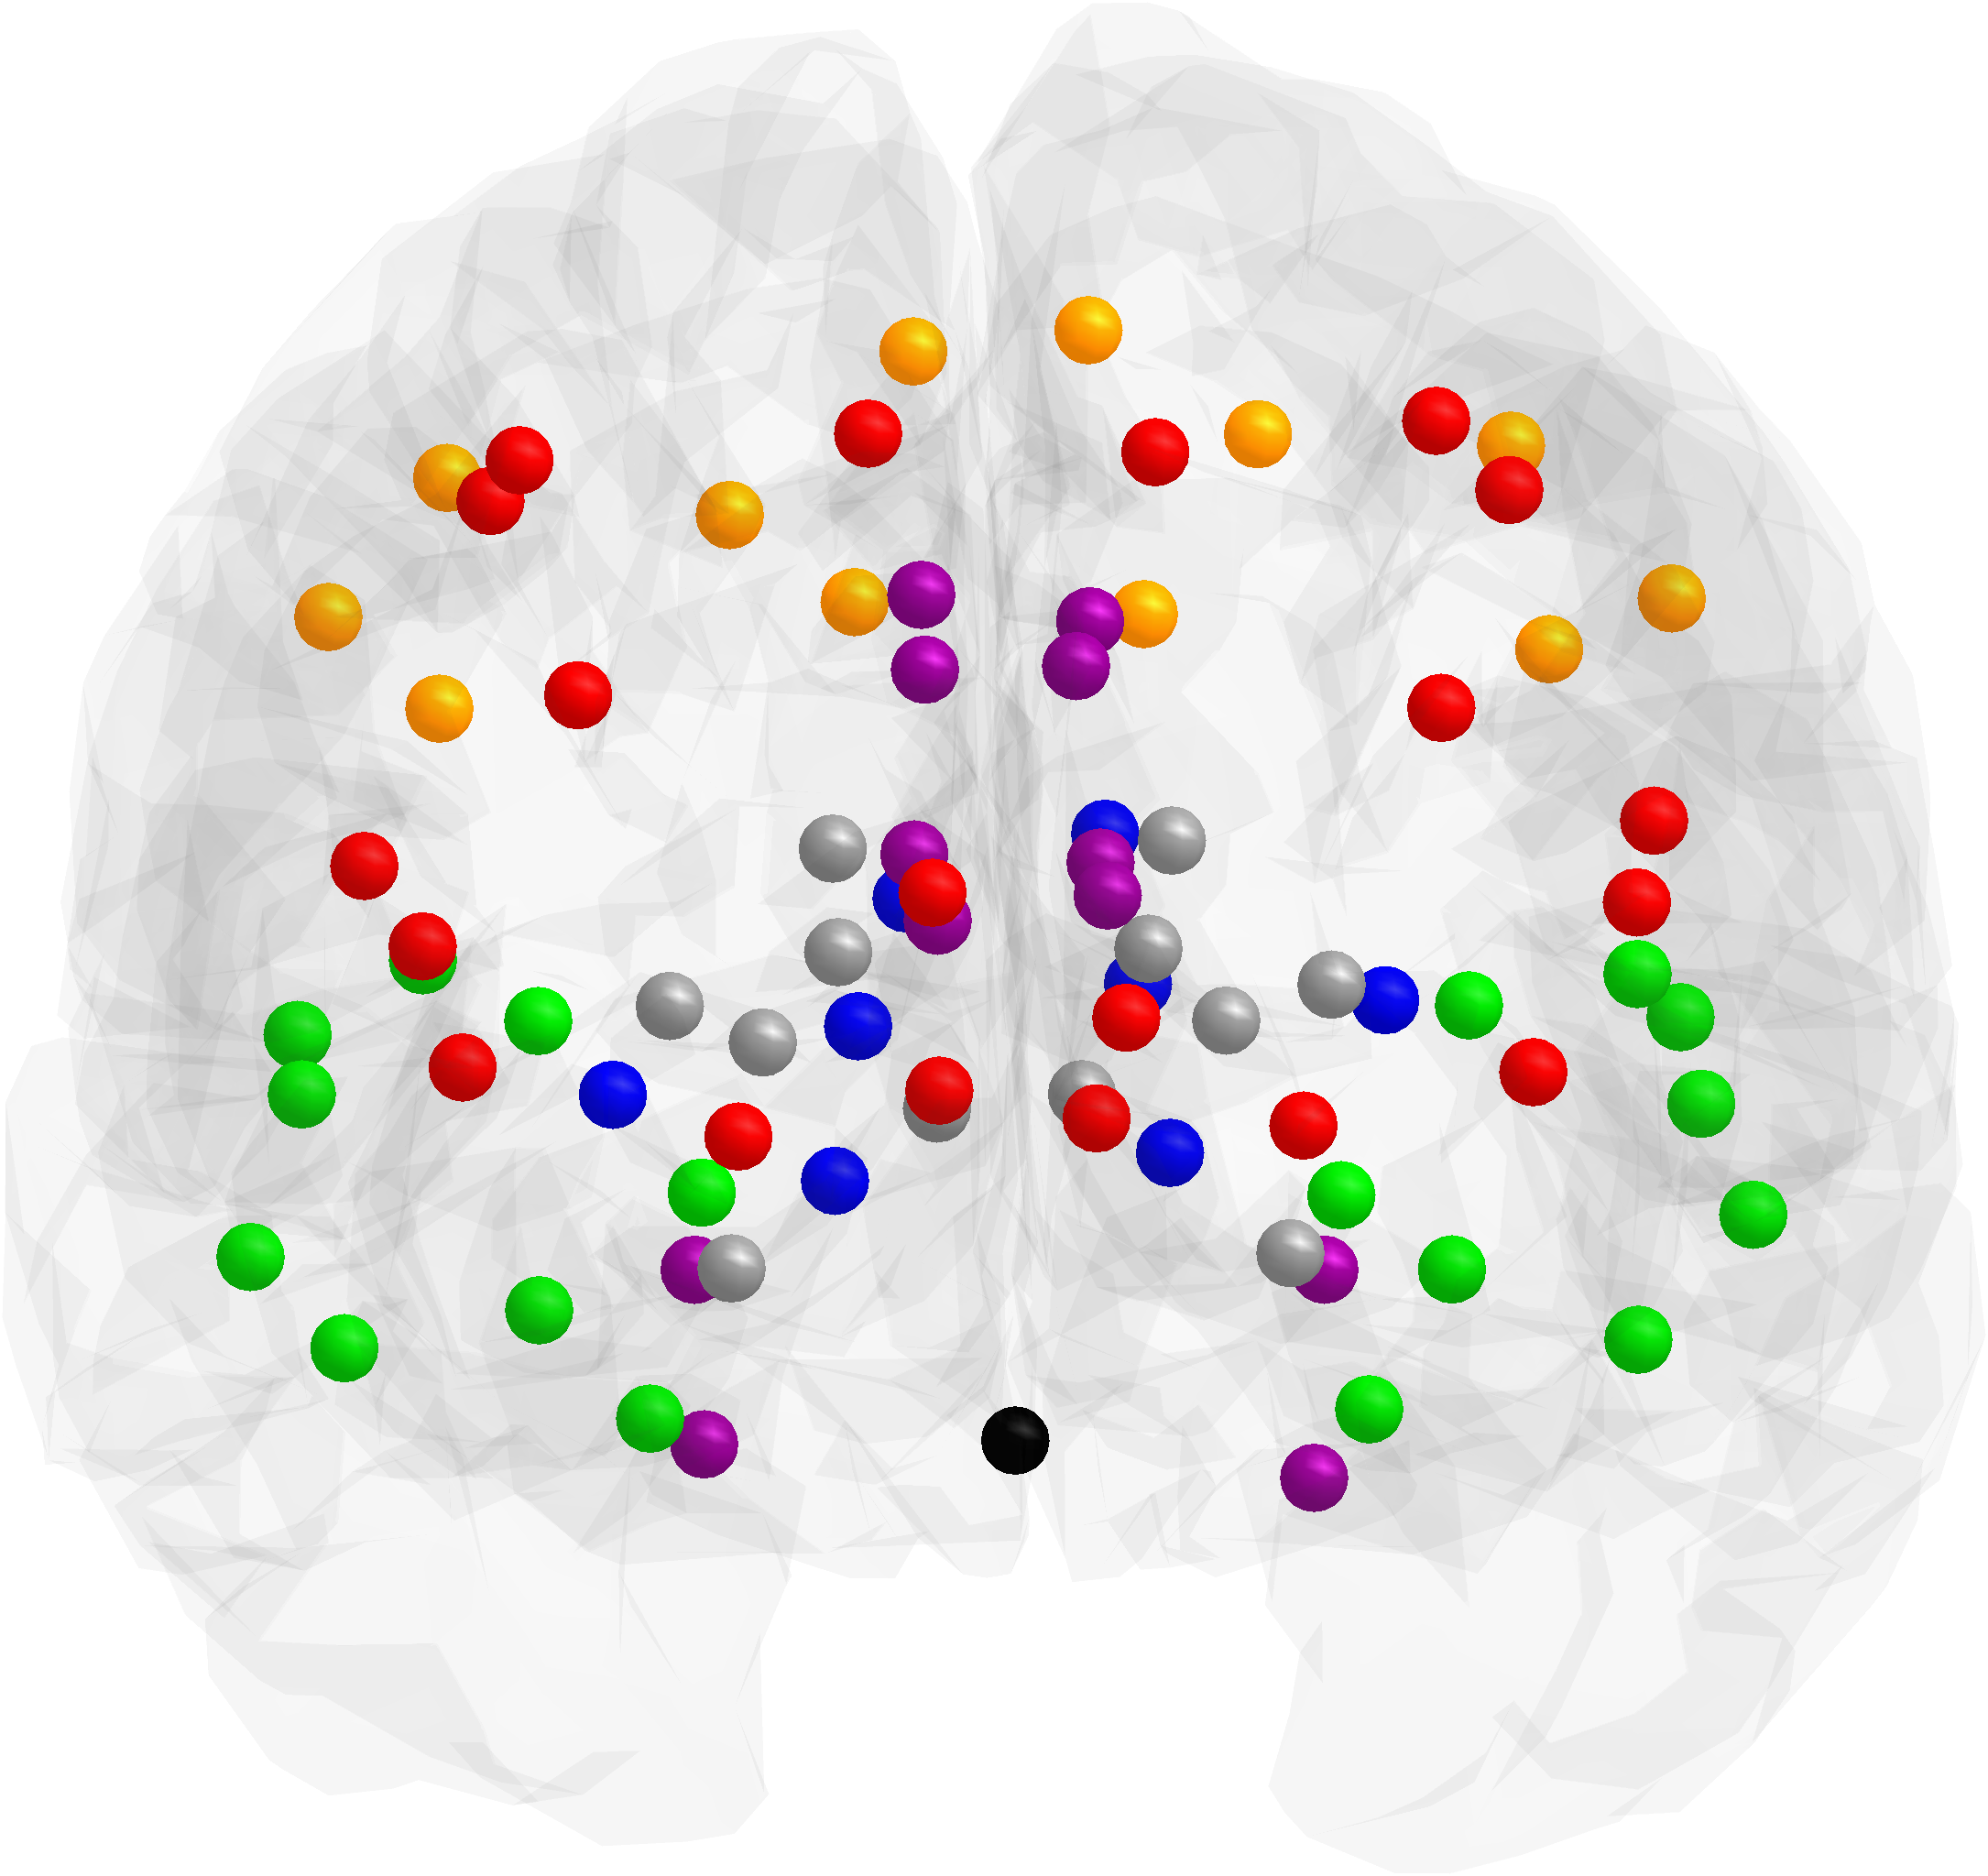
\includegraphics[width=\widthIm cm]
            {../Figure/regioniCervelloFronte [Trasparente].png}};
            % {../Figure/regioniCervelloFronte [Trasparente].png}};
        \node[anchor=north west] at (FKR c1r3.north west)
            {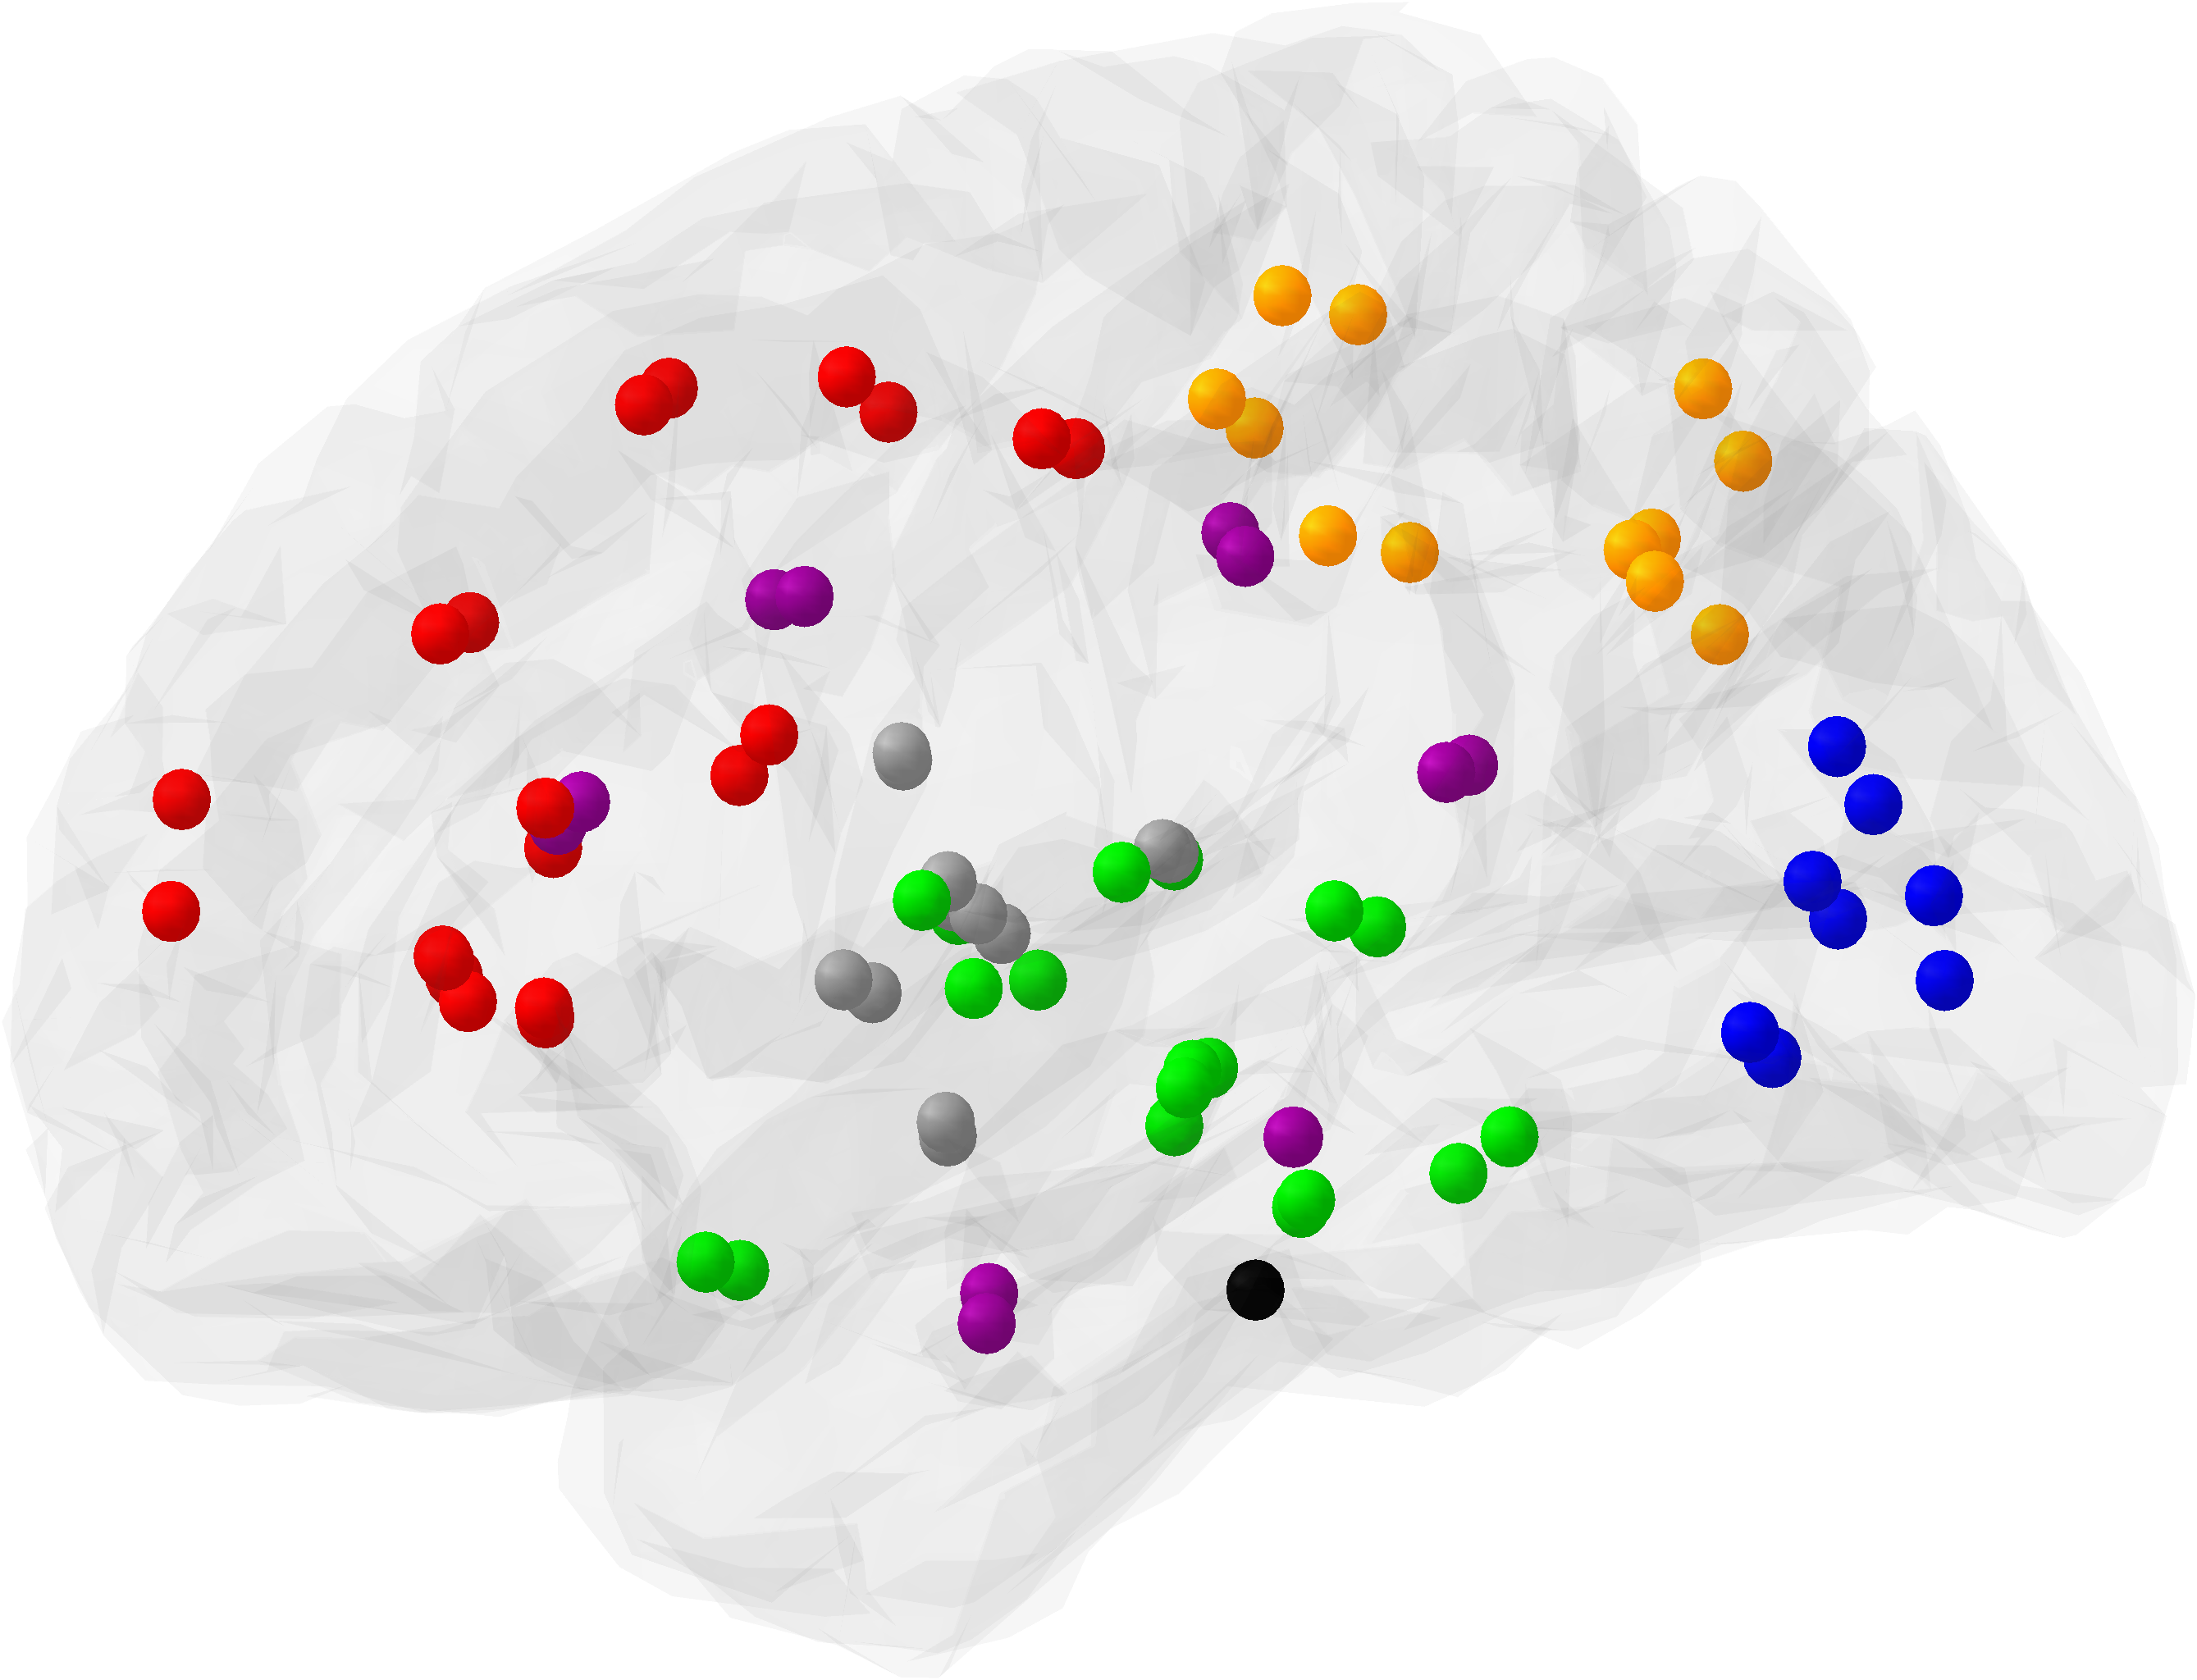
\includegraphics[width=\widthIm cm]
            {../Figure/regioniCervelloLato [Trasparente].png}};
            % {../Figure/regioniCervelloLato [Trasparente].png}};
        \node[anchor=north west] at (FKR c1r4.north west)
            {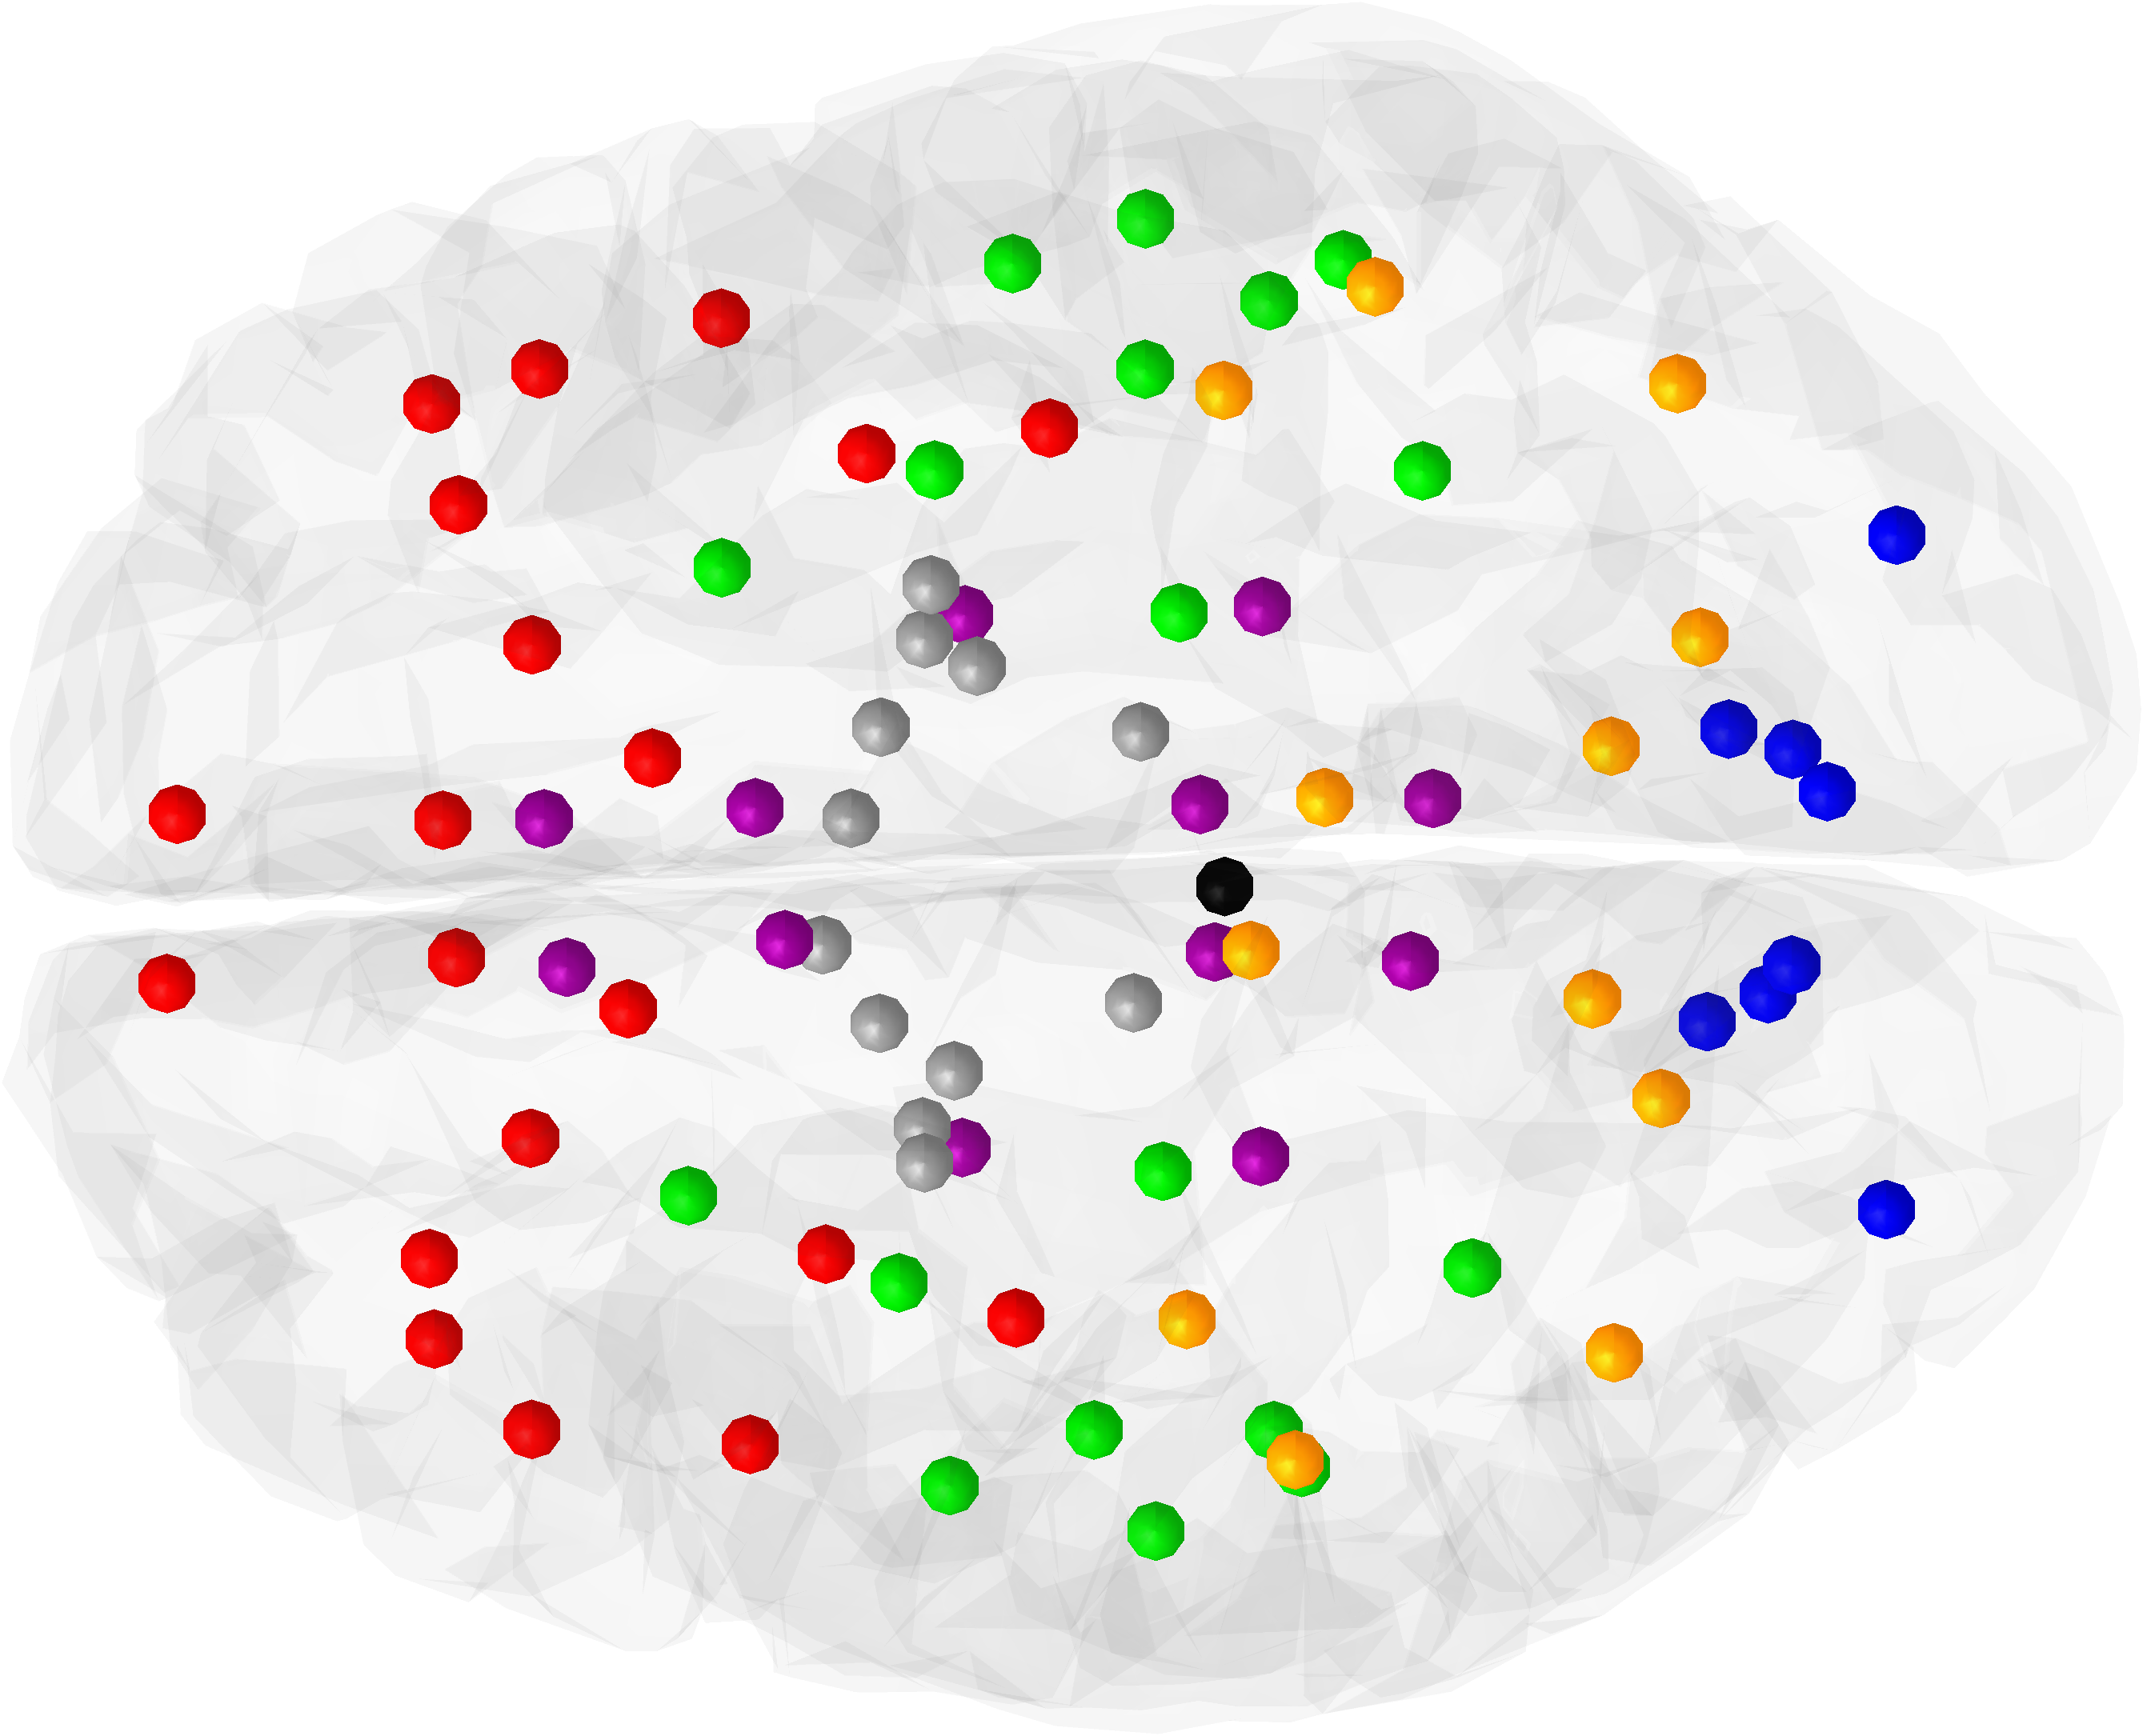
\includegraphics[width=\widthIm cm]
            {../Figure/regioniCervelloAlto [Trasparente].png}};
            % {../Figure/regioniCervelloAlto [Trasparente].png}};

        %
        \tikzset{SubCaption/.style={text width=4cm,anchor=south east,align=right}} %,inner sep=0pt,draw
        \node[SubCaption] at (FKR c1r1.south east)
            {\dimTesto{\captionSize}\sottoDidascalia{\selezionaLingua{$\mathbf L$ statica}{Static $\mathbf L$}\label{figFKStaticL}}};
        \node[SubCaption] at (FKR c1r2.south east)
            {\dimTesto{\captionSize}\sottoDidascalia{\selezionaLingua{$\mathbf L$ dinamica}{Dynamic $\mathbf L$}\label{figFKDynamicL}}};
        \node[SubCaption] at (FKR c1r3.south east)
            {\dimTesto{\captionSize}\sottoDidascalia{\selezionaLingua{Variante}{Variant} $f_d^l\leftrightarrow f_d^h$\label{figFKDynamicLVariant1}}};
        \node[SubCaption] at (FKR c1r4.south east)
            {\dimTesto{\captionSize}\sottoDidascalia{\selezionaLingua{Variante}{Variant} $f_d^l\leftrightarrow f_d^m$\label{figFKDynamicLVariant2}}};

        \node[SubCaption] at (FKN c1r1.south east)
            {\dimTesto{\captionSize}\sottoDidascalia{\selezionaLingua{Rete}{Network}\label{figFKNetwork}}};
        \node[SubCaption] at (FKN c1r2.south east)
            {\dimTesto{\captionSize}\sottoDidascalia{\selezionaLingua{Temporale}{Temporal}\label{figFKTemporal}}};
        \node[SubCaption] at (FKN c1r3.south east)
            {\dimTesto{\captionSize}\sottoDidascalia{\selezionaLingua{Frontale}{Frontal}\label{figFKFrontal}}};
        \node[SubCaption] at (FKN c1r4.south east)
            {\dimTesto{\captionSize}\sottoDidascalia{\selezionaLingua{Parietale}{Parietal}\label{figFKParietal}}};
        \node[SubCaption] at (FKN c1r5.south east)
            {\dimTesto{\captionSize}\sottoDidascalia{\selezionaLingua{Occipitale}{Occipital}\label{figFKOccipital}}};
        \node[SubCaption] at (FKN c1r6.south east)
            {\dimTesto{\captionSize}\sottoDidascalia{\selezionaLingua{Limbico}{Limbic}\label{figFKLimbic}}};
        \node[SubCaption] at (FKN c1r7.south east)
            {\dimTesto{\captionSize}\sottoDidascalia{\selezionaLingua{Ganglia basale}{Basal ganglia}\label{figFKBasalGanglia}}};
        \node[SubCaption] at (FKN c1r8.south east)
            {\dimTesto{\captionSize}\sottoDidascalia{\selezionaLingua{Ceppo enfalico}{Brainstem}\label{figFKBrainstem}}};

        % Un'alternativa a quella di aumentare il contantore delle figure prima di «tikzpicture», usare la funzione «\sottoDidascalia{}» e di decrementare il contatore dopo «tikzpicture» è quella di usare «\subcaptionbox{}»
        % https://tex.stackexchange.com/questions/632045/get-subcaption-for-every-plot-using-groupplot-pgf-tikz-after-2020-update
        % Tuttavia il problema è che a volte LaTeX si lamenta con «nullfont», seppure vi sia testo all'interno della didascalia, e che essa non è rigida: non si possono controllare l'allineamento e la dimensione del nodo perfettamente
        % Un'altra possibilità è di scrivere «\caption» o «\captionof» prima della figure flottante e trattare la didascalia come un titolo della figura
    \end{tikzpicture}
}{% Classe «beamer»
    \pgfmathsetmacro\titleSize{14.4} % Dimensione del titolo
    \pgfmathsetmacro\captionSize{12} % Dimensione dell'etichette
    \pgfmathsetmacro\labelSize{12} % Dimensione dell'etichette
    \pgfmathsetmacro\tickSize{12} % Dimensioni delle tacche
    \pgfmathsetmacro\legendSize{9} % Dimensione della legenda

    %
    
    \pgfmathsetmacro\widthPlot{10}
    \pgfmathsetmacro\heightPlot{.6*\widthPlot}
    \pgfmathsetmacro\xSep{.5}
    \pgfmathsetmacro\ySep{.5}

    %

    \pgfmathsetmacro\lineWidth{.75}

    \tikzset{SubCaption/.style={text width=4cm,anchor=south east,align=right}} %,inner sep=0pt,draw

    \begin{frame}\frametitle{\insertsection{} - \insertsubsection{}}
        \begin{figure}[h!]
            \centering
            % \fbox{
            \makebox[\textwidth][c]{
            \resizebox{1.15\textwidth}{!}{
                \begin{tikzpicture}
                    \pgfmathsetmacro\xSep{.3}
                    \begin{groupplot}[
                        group style={
                            group name=FKR, % FK Regioni
                            group size=2 by 2,
                            vertical sep=\ySep cm,
                            horizontal sep=\xSep cm,
                            xlabels at=edge bottom,
                            ylabels at=edge left,
                            xticklabels at=edge bottom,
                            yticklabels at=edge left,
                            % x descriptions at=edge bottom
                        },
                        width=\widthPlot cm,
                        height=\heightPlot cm,
                        scale only axis,% Fondamentale per avere coerenza tra i due grafici,altrimenti non scalano correttamente
                        xmin=0,xmax=30,
                        xlabel={$t$ [\unit{\year}]},
                        xlabel style={
                            font=\color{white!15!black}\dimTesto{\labelSize},
                            yshift=.15cm,
                            % at={(ticklabel cs:1.0)},
                            % anchor=east,
                        },
                        ymin=0,ymax=1,
                        ylabel={$c$ [\%]},
                        ylabel style={
                            font=\color{white!15!black}\dimTesto{\labelSize},
                            yshift=-.15cm,
                            % at={(ticklabel cs:1.0)},
                            % anchor=east,
                        },
                        xticklabel style={
                            font=\dimTesto{\tickSize},
                            anchor=north
                        },
                        yticklabel style={
                            font=\dimTesto{\tickSize},
                            anchor=east
                        },
                        ytick distance=0.1,
                        axis x line*=bottom,
                        axis y line*=left,
                        xmajorgrids,
                        ymajorgrids,
                        grid style={dashed},
                    ]
                        \nextgroupplot[ % 1
                                        % title style={font=\bfseries\tSizeTitle},
                                        % title={\selezionaLingua{Modello \FKdiscrete{}}{\FKdiscrete{} model}},
                                        legend style={legend cell align=left,
                                                    align=left,
                                                    legend pos=north west,
                                                    draw=white!15!black,
                                                    font=\dimTesto{\legendSize},
                                                    % fill=none,
                                                    % draw=none,
                                                    },
                                    ]
                        %\begingroup % Statico
                        \addplot [color=black,dashed,line width=\lineWidth pt]
                            table[row sep=crcr]{%
                        0	0.00240963855421687\\
                        0.4	0.00292466694502703\\
                        0.8	0.0035305179861389\\
                        1.2	0.00423575301794201\\
                        1.6	0.00504723498398097\\
                        2	0.00596943575665603\\
                        2.4	0.0070039357199673\\
                        2.8	0.00814928980826181\\
                        3.2	0.00940141280649762\\
                        3.6	0.0107545683067735\\
                        4	0.0122029430445418\\
                        4.4	0.0137426815454279\\
                        4.8	0.0153741809372719\\
                        5.2	0.0171044273807985\\
                        5.6	0.0189491963543618\\
                        6	0.0209350192977185\\
                        6.4	0.0231009077937645\\
                        6.8	0.0254998949309808\\
                        7.2	0.0282004848774309\\
                        7.6	0.0312880926644432\\
                        8	0.0348665130872463\\
                        8.4	0.0390593910331553\\
                        8.8	0.0440115859207475\\
                        9.2	0.0498902386293929\\
                        9.6	0.0568852662403692\\
                        10	0.0652089321886681\\
                        10.4	0.0750940704958346\\
                        10.8	0.0867904876309486\\
                        11.2	0.10055903446945\\
                        11.6	0.116662853917144\\
                        12	0.135355400497112\\
                        12.4	0.156865041896279\\
                        12.8	0.181376436304291\\
                        13.2	0.209009461483885\\
                        13.6	0.239797230657553\\
                        14	0.27366556384345\\
                        14.4	0.310416990722958\\
                        14.8	0.349722666286264\\
                        15.2	0.391125208620723\\
                        15.6	0.434054267034464\\
                        16	0.477854688437143\\
                        16.4	0.521824851855364\\
                        16.8	0.565260681983756\\
                        17.2	0.607499646096211\\
                        17.6	0.64795907033437\\
                        18	0.686164370104303\\
                        18.4	0.721764866878947\\
                        18.8	0.754537130164705\\
                        19.2	0.784377644312435\\
                        19.6	0.811287703587221\\
                        20	0.835353742069713\\
                        20.4	0.856725998020483\\
                        20.8	0.875597777061739\\
                        21.2	0.892186863129063\\
                        21.6	0.906719983868784\\
                        22	0.919420726658972\\
                        22.4	0.930500920517231\\
                        22.8	0.940155222609388\\
                        23.2	0.948558453341346\\
                        23.6	0.955865100622207\\
                        24	0.962210360830602\\
                        24.4	0.967712101522178\\
                        24.8	0.972473212388698\\
                        25.2	0.976583938997016\\
                        25.6	0.980123942011195\\
                        26	0.983163964488135\\
                        26.4	0.985767099239553\\
                        26.8	0.987989716732732\\
                        27.2	0.989882143197788\\
                        27.6	0.991489178331673\\
                        28	0.992850524801783\\
                        28.4	0.994001178674119\\
                        28.8	0.994971808297686\\
                        29.2	0.99578913267496\\
                        29.6	0.996476299730036\\
                        30	0.997053259343402\\
                        };
                        \addlegendentry{\selezionaLingua{Rete}{Network}}
                        
                        \addplot [color=mycolor1,line width=\lineWidth pt]
                            table[row sep=crcr]{%
                        0	0\\
                        0.4	7.04171308036035e-05\\
                        0.8	0.0001672048701582\\
                        1.2	0.000297593640187364\\
                        1.6	0.00047039001380224\\
                        2	0.000696245355283955\\
                        2.4	0.000987971062312688\\
                        2.8	0.00136091844256661\\
                        3.2	0.00183344759533614\\
                        3.6	0.00242751517133344\\
                        4	0.00316941440823133\\
                        4.4	0.00409070162785883\\
                        4.8	0.0052293412150801\\
                        5.2	0.00663109608624231\\
                        5.6	0.00835118270409559\\
                        6	0.0104561978995357\\
                        6.4	0.0130263069503838\\
                        6.8	0.0161576549879967\\
                        7.2	0.0199649221440234\\
                        7.6	0.0245838816769949\\
                        8	0.0301737350345084\\
                        8.4	0.0369188864319131\\
                        8.8	0.0450296858238938\\
                        9.2	0.0547415269701936\\
                        9.6	0.0663115655831579\\
                        10	0.0800122689302831\\
                        10.4	0.0961210876435254\\
                        10.8	0.114905823369919\\
                        11.2	0.136605802613332\\
                        11.6	0.161409749715729\\
                        12	0.189432177122574\\
                        12.4	0.220690968895706\\
                        12.8	0.255089347296453\\
                        13.2	0.292405334188646\\
                        13.6	0.332291046145129\\
                        14	0.374282810570177\\
                        14.4	0.417821474873627\\
                        14.8	0.462280801846695\\
                        15.2	0.507000837509718\\
                        15.6	0.551322761367464\\
                        16	0.594621937569825\\
                        16.4	0.636336489351372\\
                        16.8	0.67598949571434\\
                        17.2	0.7132037021458\\
                        17.6	0.747708388245802\\
                        18	0.779338741329222\\
                        18.4	0.808028728214549\\
                        18.8	0.833798971665503\\
                        19.2	0.856741436625102\\
                        19.6	0.877002761950399\\
                        20	0.894767852409514\\
                        20.4	0.910244952625648\\
                        20.8	0.923652965638926\\
                        21.2	0.935211348637565\\
                        21.6	0.945132577492984\\
                        22	0.953616942421088\\
                        22.4	0.960849312865095\\
                        22.8	0.966997468289305\\
                        23.2	0.972211606252168\\
                        23.6	0.976624685770624\\
                        24	0.980353324228943\\
                        24.4	0.983499027729118\\
                        24.8	0.986149590853747\\
                        25.2	0.988380549116205\\
                        25.6	0.990256605153319\\
                        26	0.991832978589689\\
                        26.4	0.993156650736052\\
                        26.8	0.994267490329683\\
                        27.2	0.995199256770151\\
                        27.6	0.995980483956098\\
                        28	0.996635251872115\\
                        28.4	0.9971838552805\\
                        28.8	0.997643379824352\\
                        29.2	0.998028195975112\\
                        29.6	0.998350380868087\\
                        30	0.998620077379581\\
                        };
                        \addlegendentry{\selezionaLingua{Temporale}{Temporal}}
                        
                        \addplot [color=black!20!red,line width=\lineWidth pt]
                            table[row sep=crcr]{%
                        0	0\\
                        0.4	7.45220646300236e-07\\
                        0.8	2.66053818596183e-06\\
                        1.2	6.33256066900219e-06\\
                        1.6	1.25599498691122e-05\\
                        2	2.24173470551563e-05\\
                        2.4	3.73363879315031e-05\\
                        2.8	5.92082605309682e-05\\
                        3.2	9.0513507711793e-05\\
                        3.6	0.000134486352877914\\
                        4	0.000195322780129838\\
                        4.4	0.000278443973293844\\
                        4.8	0.000390829557993377\\
                        5.2	0.000541438442021968\\
                        5.6	0.000741738944577451\\
                        6	0.00100637433954323\\
                        6.4	0.00135399482479046\\
                        6.8	0.00180829203008117\\
                        7.2	0.00239927699995348\\
                        7.6	0.00316484624780737\\
                        8	0.00415268148980219\\
                        8.4	0.00542252468862067\\
                        8.8	0.00704885754264351\\
                        9.2	0.00912398850054889\\
                        9.6	0.0117615039533295\\
                        10	0.0150999649500406\\
                        10.4	0.0193066172028745\\
                        10.8	0.0245807221693896\\
                        11.2	0.0311559081354635\\
                        11.6	0.039300692918927\\
                        12	0.049316077679901\\
                        12.4	0.0615289222557084\\
                        12.8	0.0762797949966285\\
                        13.2	0.0939042850401585\\
                        13.6	0.114707509671452\\
                        14	0.138932808211049\\
                        14.4	0.166727286534176\\
                        14.8	0.198108626659432\\
                        15.2	0.232938846196642\\
                        15.6	0.270910855937973\\
                        16	0.311552298422199\\
                        16.4	0.35424831525503\\
                        16.8	0.398281235287812\\
                        17.2	0.442881758740523\\
                        17.6	0.487284085238452\\
                        18	0.530777186562522\\
                        18.4	0.572745950288165\\
                        18.8	0.61269852121596\\
                        19.2	0.650278930262996\\
                        19.6	0.685266305410928\\
                        20	0.717563301992899\\
                        20.4	0.747176945499526\\
                        20.8	0.7741951081684\\
                        21.2	0.798761585881849\\
                        21.6	0.821052339375135\\
                        22	0.841254948589519\\
                        22.4	0.859552699220945\\
                        22.8	0.876113995913308\\
                        23.2	0.891087044725842\\
                        23.6	0.904599073640304\\
                        24	0.916758874154351\\
                        24.4	0.927661227030982\\
                        24.8	0.937391838416012\\
                        25.2	0.946031708062134\\
                        25.6	0.953660276501559\\
                        26	0.960357132826855\\
                        26.4	0.966202411347959\\
                        26.8	0.971276213282269\\
                        27.2	0.975657458641542\\
                        27.6	0.979422538204022\\
                        28	0.982644043066933\\
                        28.4	0.985389741598044\\
                        28.8	0.98772187833009\\
                        29.2	0.989696799294941\\
                        29.6	0.991364865235348\\
                        30	0.992770593646474\\
                        };
                        \addlegendentry{\selezionaLingua{Frontale}{Frontal}}
                        
                        \addplot [color=mycolor2,line width=\lineWidth pt]
                            table[row sep=crcr]{%
                        0	0\\
                        0.4	2.92265476511174e-06\\
                        0.8	9.40518562876677e-06\\
                        1.2	2.11048749342142e-05\\
                        1.6	4.02366709361726e-05\\
                        2	6.97272979876758e-05\\
                        2.4	0.000113406548683666\\
                        2.8	0.000176244567594364\\
                        3.2	0.000264646276215627\\
                        3.6	0.000386816955089738\\
                        4	0.00055321638479435\\
                        4.4	0.000777122808317764\\
                        4.8	0.00107533222978286\\
                        5.2	0.00146902306663044\\
                        5.6	0.00198482067286097\\
                        6	0.00265610029765942\\
                        6.4	0.00352456984877615\\
                        6.8	0.0046421740898302\\
                        7.2	0.00607335757215646\\
                        7.6	0.00789771164357652\\
                        8	0.0102130069863852\\
                        8.4	0.0131385715675113\\
                        8.8	0.0168189074970138\\
                        9.2	0.0214273411411663\\
                        9.6	0.0271693617230256\\
                        10	0.0342851212162599\\
                        10.4	0.0430503483346461\\
                        10.8	0.053774694208459\\
                        11.2	0.0667963248249777\\
                        11.6	0.0824714860411251\\
                        12	0.101157903195761\\
                        12.4	0.123191365209491\\
                        12.8	0.148855779982422\\
                        13.2	0.178348375905374\\
                        13.6	0.211743397961176\\
                        14	0.248959235883844\\
                        14.4	0.289734896840175\\
                        14.8	0.333621560856095\\
                        15.2	0.379993320328419\\
                        15.6	0.42807821871976\\
                        16	0.477006975096589\\
                        16.4	0.525873271920579\\
                        16.8	0.573797192503298\\
                        17.2	0.619982987431876\\
                        17.6	0.66376389807393\\
                        18	0.704629727622626\\
                        18.4	0.742236302676278\\
                        18.8	0.776398977174573\\
                        19.2	0.80707427281026\\
                        19.6	0.834334449763388\\
                        20	0.858339462781084\\
                        20.4	0.879309781313148\\
                        20.8	0.897502351362459\\
                        21.2	0.913190857608473\\
                        21.6	0.926650572753019\\
                        22	0.93814750224454\\
                        22.4	0.947931216004537\\
                        22.8	0.956230640130978\\
                        23.2	0.963252092054258\\
                        23.6	0.969178924591652\\
                        24	0.974172256203058\\
                        24.4	0.978372380181509\\
                        24.8	0.981900550126023\\
                        25.2	0.984860926612604\\
                        25.6	0.987342539274719\\
                        26	0.989421170970223\\
                        26.4	0.991161108952617\\
                        26.8	0.99261673485053\\
                        27.2	0.993833943457655\\
                        27.6	0.994851392113722\\
                        28	0.995701589630883\\
                        28.4	0.996411837687823\\
                        28.8	0.997005039416934\\
                        29.2	0.997500390303285\\
                        29.6	0.997913966032709\\
                        30	0.998259220939409\\
                        };
                        \addlegendentry{\selezionaLingua{Parietale}{Parietal}}
                        
                        \addplot [color=black!20!blue,line width=\lineWidth pt]
                            table[row sep=crcr]{%
                        0	0\\
                        0.4	1.82060656035207e-06\\
                        0.8	5.93546786075404e-06\\
                        1.2	1.3535149714226e-05\\
                        1.6	2.62564063765374e-05\\
                        2	4.63198496737192e-05\\
                        2.4	7.67048465576088e-05\\
                        2.8	0.000121371193016474\\
                        3.2	0.000185539621371701\\
                        3.6	0.000276046287662253\\
                        4	0.000401790097831203\\
                        4.4	0.000574296078118148\\
                        4.8	0.000808422946487718\\
                        5.2	0.0011232484950284\\
                        5.6	0.00154317211057173\\
                        6	0.00209927926737387\\
                        6.4	0.00283101725449778\\
                        6.8	0.0037882332774128\\
                        7.2	0.00503362303460818\\
                        7.6	0.00664562631834375\\
                        8	0.00872178092271543\\
                        8.4	0.0113825000627452\\
                        8.8	0.0147751626203263\\
                        9.2	0.0190782896449038\\
                        9.6	0.0245054152992107\\
                        10	0.0313080415766974\\
                        10.4	0.0397768016856234\\
                        10.8	0.0502396778240764\\
                        11.2	0.0630558905817705\\
                        11.6	0.0786040071998352\\
                        12	0.0972630483997523\\
                        12.4	0.119386055925107\\
                        12.8	0.145266799817094\\
                        13.2	0.175101987890487\\
                        13.6	0.208953196817163\\
                        14	0.246714259973845\\
                        14.4	0.288090411383484\\
                        14.8	0.332594625075345\\
                        15.2	0.379564217671357\\
                        15.6	0.428197327019633\\
                        16	0.477605201203054\\
                        16.4	0.526873332869037\\
                        16.8	0.575123121278995\\
                        17.2	0.621566192577696\\
                        17.6	0.665545454648151\\
                        18	0.706559740242626\\
                        18.4	0.744271758454216\\
                        18.8	0.778501438923304\\
                        19.2	0.809208277327268\\
                        19.6	0.836466892851927\\
                        20	0.86043981181043\\
                        20.4	0.881350747551064\\
                        20.8	0.899460645939794\\
                        21.2	0.915047760766625\\
                        21.6	0.928392183110779\\
                        22	0.939764648553332\\
                        22.4	0.949419087565458\\
                        22.8	0.957588224803861\\
                        23.2	0.964481513698706\\
                        23.6	0.970284757621117\\
                        24	0.97516087401194\\
                        24.4	0.979251373183994\\
                        24.8	0.982678231460651\\
                        25.2	0.985545930404999\\
                        25.6	0.987943507576051\\
                        26	0.98994652035108\\
                        26.4	0.991618865306845\\
                        26.8	0.993014424388878\\
                        27.2	0.994178528446246\\
                        27.6	0.995149241116172\\
                        28	0.995958473487732\\
                        28.4	0.996632943983296\\
                        28.8	0.997194999607074\\
                        29.2	0.997663314942805\\
                        29.6	0.998053484614555\\
                        30	0.998378523751185\\
                        };
                        \addlegendentry{\selezionaLingua{Occipitale}{Occipital}}
                        
                        \addplot [color=mycolor3,line width=\lineWidth pt]
                            table[row sep=crcr]{%
                        0	0.0166666666666667\\
                        0.4	0.0200992326918299\\
                        0.8	0.0241027202126695\\
                        1.2	0.0287184684025896\\
                        1.6	0.0339715450849588\\
                        2	0.0398649948263497\\
                        2.4	0.0463752166314561\\
                        2.8	0.0534496166861671\\
                        3.2	0.0610075150679834\\
                        3.6	0.0689447932395947\\
                        4	0.0771420416528328\\
                        4.4	0.0854752137946924\\
                        4.8	0.0938272629742232\\
                        5.2	0.102099103874768\\
                        5.6	0.110218520470722\\
                        6	0.118146201696525\\
                        6.4	0.125878716820982\\
                        6.8	0.133448755101604\\
                        7.2	0.140923245352964\\
                        7.6	0.148400033961302\\
                        8	0.156003697567462\\
                        8.4	0.163880891080909\\
                        8.8	0.172195469932947\\
                        9.2	0.181123538472239\\
                        9.6	0.190848587099109\\
                        10	0.201556967075997\\
                        10.4	0.213434045793758\\
                        10.8	0.226661384727412\\
                        11.2	0.24141508573155\\
                        11.6	0.257865011181999\\
                        12	0.276173960662504\\
                        12.4	0.296495272771533\\
                        12.8	0.318966999627551\\
                        13.2	0.343701054290659\\
                        13.6	0.370766709516075\\
                        14	0.400169449878699\\
                        14.4	0.431828097938791\\
                        14.8	0.465554780712995\\
                        15.2	0.501043039472702\\
                        15.6	0.537868735246314\\
                        16	0.575506276357419\\
                        16.4	0.61335952736467\\
                        16.8	0.650803433451528\\
                        17.2	0.687229941397194\\
                        17.6	0.722090985208115\\
                        18	0.754932316312689\\
                        18.4	0.785414343883835\\
                        18.8	0.813319057206106\\
                        19.2	0.838544656328377\\
                        19.6	0.861091148221635\\
                        20	0.881040725138432\\
                        20.4	0.898536426742242\\
                        20.8	0.913761759227485\\
                        21.2	0.926922958868122\\
                        21.6	0.938234695974152\\
                        22	0.947909343444594\\
                        22.4	0.956149506683956\\
                        22.8	0.963143293818586\\
                        23.2	0.969061739133001\\
                        23.6	0.97405782107693\\
                        24	0.97826659325691\\
                        24.4	0.981806041001166\\
                        24.8	0.984778368415458\\
                        25.2	0.98727150172881\\
                        25.6	0.989360660627346\\
                        26	0.9911099002028\\
                        26.4	0.99257356383761\\
                        26.8	0.993797614199252\\
                        27.2	0.994820827923464\\
                        27.6	0.995675851658788\\
                        28	0.996390124671989\\
                        28.4	0.99698667753919\\
                        28.8	0.997484818597489\\
                        29.2	0.997900720553684\\
                        29.6	0.998247919472148\\
                        30	0.998537737660752\\
                        };
                        \addlegendentry{\selezionaLingua{Limbico}{Limbic}}
                        
                        \addplot [color=mycolor4,line width=\lineWidth pt]
                            table[row sep=crcr]{%
                        0	0\\
                        0.4	1.85701263021213e-05\\
                        0.8	4.75839376698943e-05\\
                        1.2	9.04937342308951e-05\\
                        1.6	0.000151644027828696\\
                        2	0.000236459234872841\\
                        2.4	0.000351666710830223\\
                        2.8	0.000505563925256571\\
                        3.2	0.000708341314592617\\
                        3.6	0.000972475203933601\\
                        4	0.00131320781815637\\
                        4.4	0.00174913349499254\\
                        4.8	0.00230291154020386\\
                        5.2	0.00300212656224559\\
                        5.6	0.00388031638403464\\
                        6	0.004978185365818\\
                        6.4	0.00634501650837022\\
                        6.8	0.00804028803642693\\
                        7.2	0.0101354880207756\\
                        7.6	0.0127161026007422\\
                        8	0.0158837282397257\\
                        8.4	0.0197582252528537\\
                        8.8	0.0244797881655262\\
                        9.2	0.0302107583053126\\
                        9.6	0.0371369453574391\\
                        10	0.0454681564729687\\
                        10.4	0.0554375513868101\\
                        10.8	0.0672993468180232\\
                        11.2	0.0813242845409535\\
                        11.6	0.0977921712637682\\
                        12	0.116980740658031\\
                        12.4	0.139150164671595\\
                        12.8	0.164522871967095\\
                        13.2	0.193259029885787\\
                        13.6	0.225429148852701\\
                        14	0.260986649553823\\
                        14.4	0.299744559540509\\
                        14.8	0.341361276641304\\
                        15.2	0.385340042390141\\
                        15.6	0.431045127850892\\
                        16	0.477734904526574\\
                        16.4	0.524608605338574\\
                        16.8	0.570860641882129\\
                        17.2	0.615734750594936\\
                        17.6	0.658570477177487\\
                        18	0.698836431069594\\
                        18.4	0.736147665782349\\
                        18.8	0.770267559819609\\
                        19.2	0.801096918828311\\
                        19.6	0.82865429647765\\
                        20	0.85305174364547\\
                        20.4	0.874469623112303\\
                        20.8	0.893133147364529\\
                        21.2	0.909292243233905\\
                        21.6	0.923205437300551\\
                        22	0.935127788708095\\
                        22.4	0.945302479993174\\
                        22.8	0.953955470069579\\
                        23.2	0.961292557168354\\
                        23.6	0.967498236250118\\
                        24	0.972735820111755\\
                        24.4	0.977148394953355\\
                        24.8	0.980860280649753\\
                        25.2	0.983978753638307\\
                        25.6	0.986595862420041\\
                        26	0.988790222051705\\
                        26.4	0.990628716290039\\
                        26.8	0.992168066651788\\
                        27.2	0.993456248997084\\
                        27.6	0.99453375257131\\
                        28	0.995434685593431\\
                        28.4	0.996187736946852\\
                        28.8	0.996817006436297\\
                        29.2	0.997342717264516\\
                        29.6	0.997781824464764\\
                        30	0.998148532427392\\
                        };
                        \addlegendentry{\selezionaLingua{Gangli basali}{Basal ganglia}}
                        
                        \addplot [color=black,line width=\lineWidth pt]
                            table[row sep=crcr]{%
                        0	0\\
                        0.4	1.67314260489531e-06\\
                        0.8	6.0986484569721e-06\\
                        1.2	1.50784136640532e-05\\
                        1.6	3.11237689017505e-05\\
                        2	5.76693583239417e-05\\
                        2.4	9.93404129266556e-05\\
                        2.8	0.000162285216563665\\
                        3.2	0.000254587192542397\\
                        3.6	0.000386774235925593\\
                        4	0.000572446694152876\\
                        4.4	0.000829049702202057\\
                        4.8	0.00117882025983837\\
                        5.2	0.00164994420952393\\
                        5.6	0.00227796263077473\\
                        6	0.0031074702691043\\
                        6.4	0.00419414910621801\\
                        6.8	0.00560717593220798\\
                        7.2	0.00743203060765554\\
                        7.6	0.00977370699252542\\
                        8	0.0127602849196479\\
                        8.4	0.0165467508877907\\
                        8.8	0.0213188476306342\\
                        9.2	0.0272965785813046\\
                        9.6	0.0347367858386494\\
                        10	0.0439339621172637\\
                        10.4	0.0552181698457653\\
                        10.8	0.0689486776830608\\
                        11.2	0.0855017853911556\\
                        11.6	0.105251442419915\\
                        12	0.12854185806236\\
                        12.4	0.155652512921988\\
                        12.8	0.186757844525866\\
                        13.2	0.221886162857937\\
                        13.6	0.260884470038826\\
                        14	0.303396940935009\\
                        14.4	0.34886400869518\\
                        14.8	0.396545916203286\\
                        15.2	0.445569748746228\\
                        15.6	0.494993742526078\\
                        16	0.543878814190625\\
                        16.4	0.591356072131754\\
                        16.8	0.636680791762002\\
                        17.2	0.679267118840991\\
                        17.6	0.718702181859663\\
                        18	0.754742021480824\\
                        18.4	0.787294021584126\\
                        18.8	0.81639124758237\\
                        19.2	0.842163619198857\\
                        19.6	0.864809698046086\\
                        20	0.884571535293646\\
                        20.4	0.901713824027072\\
                        20.8	0.916507688283622\\
                        21.2	0.929218843940039\\
                        21.6	0.940099541513728\\
                        22	0.949383576131316\\
                        22.4	0.957283654235864\\
                        22.8	0.963990482444938\\
                        23.2	0.96967305041883\\
                        23.6	0.97447969097258\\
                        24	0.978539602775794\\
                        24.4	0.981964607492694\\
                        24.8	0.984850982594199\\
                        25.2	0.987281264421322\\
                        25.6	0.989325955664582\\
                        26	0.991045099858319\\
                        26.4	0.992489705256878\\
                        26.8	0.993703013707234\\
                        27.2	0.994721618614432\\
                        27.6	0.995576441183468\\
                        28	0.996293576853779\\
                        28.4	0.996895024989239\\
                        28.8	0.997399315002546\\
                        29.2	0.997822041570561\\
                        29.6	0.998176320708598\\
                        30	0.998473177400283\\
                        };
                        \addlegendentry{\selezionaLingua{Tronco encefalico}{Brainstem}}
                        %\endgroup
                        
                        \nextgroupplot
                        %\begingroup % Dinamico
                        \addplot [color=black,dashed,line width=\lineWidth pt]
                            table[row sep=crcr]{%
                        0	0.00240963855421687\\
                        0.4	0.00292466694502704\\
                        0.8	0.00353037670879158\\
                        1.2	0.00423501803627785\\
                        1.6	0.00504486962177752\\
                        2	0.00596341503897998\\
                        2.4	0.00699069130203136\\
                        2.8	0.00812299766545468\\
                        3.2	0.00935313412456172\\
                        3.6	0.0106712672262949\\
                        4	0.0120664078520084\\
                        4.4	0.013528364491765\\
                        4.8	0.0150499472863316\\
                        5.2	0.0166291728604336\\
                        5.6	0.0182712625796095\\
                        6	0.0199903163475126\\
                        6.4	0.0218106457016816\\
                        6.8	0.0237678314840737\\
                        7.2	0.0259096139850376\\
                        7.6	0.0282967241716398\\
                        8	0.0310037317816587\\
                        8.4	0.0341199330334353\\
                        8.8	0.0377502408297489\\
                        9.2	0.0420159845340354\\
                        9.6	0.0470554822790771\\
                        10	0.0530242199689198\\
                        10.4	0.0600944561143297\\
                        10.8	0.0684540627005338\\
                        11.2	0.0783043969133344\\
                        11.6	0.0898569652481416\\
                        12	0.103328589913761\\
                        12.4	0.118934738495996\\
                        12.8	0.136880677176187\\
                        13.2	0.157350216107628\\
                        13.6	0.180492085973639\\
                        14	0.206404433689365\\
                        14.4	0.235118507677846\\
                        14.8	0.266583204847658\\
                        15.2	0.300652607133863\\
                        15.6	0.337078775099491\\
                        16	0.375511774084155\\
                        16.4	0.415508170995283\\
                        16.8	0.456548157501425\\
                        17.2	0.498060218007879\\
                        17.6	0.53945110208768\\
                        18	0.580138009244447\\
                        18.4	0.619579526677978\\
                        18.8	0.657302064498667\\
                        19.2	0.692919274370251\\
                        19.6	0.726143061529836\\
                        20	0.756786063801989\\
                        20.4	0.784756609835957\\
                        20.8	0.810047969789708\\
                        21.2	0.832724068666\\
                        21.6	0.852903760890441\\
                        22	0.870745377224232\\
                        22.4	0.88643271219622\\
                        22.8	0.900163076037351\\
                        23.2	0.912137598233439\\
                        23.6	0.922553687808428\\
                        24	0.931599421829736\\
                        24.4	0.939449608001268\\
                        24.8	0.946263297349167\\
                        25.2	0.952182561808558\\
                        25.6	0.957332367525031\\
                        26	0.961821357287403\\
                        26.4	0.965743314764949\\
                        26.8	0.969179042995374\\
                        27.2	0.972198375115821\\
                        27.6	0.974862060847082\\
                        28	0.977223335217604\\
                        28.4	0.979329061008235\\
                        28.8	0.98122042447923\\
                        29.2	0.982933240901932\\
                        29.6	0.984497985165164\\
                        30	0.985939700196658\\
                        };
                        %\addlegendentry{Network}
                        
                        \addplot [color=mycolor1,line width=\lineWidth pt]
                            table[row sep=crcr]{%
                        0	0\\
                        0.4	7.04171308036133e-05\\
                        0.8	0.000160204478730234\\
                        1.2	0.000274229751227403\\
                        1.6	0.00041838107007992\\
                        2	0.000599771146948772\\
                        2.4	0.000826985818206162\\
                        2.8	0.00111039086316631\\
                        3.2	0.00146251417226236\\
                        3.6	0.00189852303205726\\
                        4	0.00243681822712462\\
                        4.4	0.0030997677052262\\
                        4.8	0.00391460276276395\\
                        5.2	0.0049144991126796\\
                        5.6	0.00613986352225551\\
                        6	0.00763984310680477\\
                        6.4	0.00947406724922501\\
                        6.8	0.0117146191088141\\
                        7.2	0.0144482116800851\\
                        7.6	0.0177785087049756\\
                        8	0.0218284796003422\\
                        8.4	0.0267426067031272\\
                        8.8	0.0326886713040044\\
                        9.2	0.0398587350616237\\
                        9.6	0.0484688155709467\\
                        10	0.0587566497176559\\
                        10.4	0.0709768795087045\\
                        10.8	0.0853930280250344\\
                        11.2	0.102265809186112\\
                        11.6	0.121837675999235\\
                        12	0.144314068043564\\
                        12.4	0.16984252466544\\
                        12.8	0.19849157099979\\
                        13.2	0.23023188555407\\
                        13.6	0.264922527830761\\
                        14	0.302304791355348\\
                        14.4	0.342005499594211\\
                        14.8	0.383550355568915\\
                        15.2	0.426386487991631\\
                        15.6	0.469911893314772\\
                        16	0.513508376927369\\
                        16.4	0.556574131419159\\
                        16.8	0.598552401166547\\
                        17.2	0.638953692827227\\
                        17.6	0.677370391185569\\
                        18	0.713483994678844\\
                        18.4	0.747066121817909\\
                        18.8	0.777974805250985\\
                        19.2	0.806147485508821\\
                        19.6	0.831591792853709\\
                        20	0.854374903888285\\
                        20.4	0.874612097511601\\
                        20.8	0.89245509676038\\
                        21.2	0.908080783620345\\
                        21.6	0.921680834273205\\
                        22	0.933452711425259\\
                        22.4	0.94359228451148\\
                        22.8	0.952288167008613\\
                        23.2	0.959717700773094\\
                        23.6	0.966044403105609\\
                        24	0.971416628952578\\
                        24.4	0.975967181781242\\
                        24.8	0.979813619876049\\
                        25.2	0.983059037060147\\
                        25.6	0.985793137333963\\
                        26	0.988093464064791\\
                        26.4	0.990026681654189\\
                        26.8	0.991649838940975\\
                        27.2	0.99301156845475\\
                        27.6	0.994153194441266\\
                        28	0.995109736205768\\
                        28.4	0.995910802767694\\
                        28.8	0.996581381050122\\
                        29.2	0.9971425236734\\
                        29.6	0.997611944562676\\
                        30	0.998004531541114\\
                        };
                        %\addlegendentry{Temporal}
                        
                        \addplot [color=black!20!red,line width=\lineWidth pt]
                            table[row sep=crcr]{%
                        0	0\\
                        0.4	7.45220646300334e-07\\
                        0.8	2.50679278954728e-06\\
                        1.2	5.65142289330294e-06\\
                        1.6	1.06678866297409e-05\\
                        2	1.82009662273744e-05\\
                        2.4	2.90947218676351e-05\\
                        2.8	4.44475154788143e-05\\
                        3.2	6.56818596222808e-05\\
                        3.6	9.46329718363549e-05\\
                        4	0.000133660906452178\\
                        4.4	0.000185792347093542\\
                        4.8	0.000254899614780255\\
                        5.2	0.000345926223822681\\
                        5.6	0.000465170445608714\\
                        6	0.000620640856273798\\
                        6.4	0.000822500764773039\\
                        6.8	0.00108362171881381\\
                        7.2	0.00142026987133137\\
                        7.6	0.0018529526450829\\
                        8	0.00240745645613401\\
                        8.4	0.00311610856377635\\
                        8.8	0.00401929630607221\\
                        9.2	0.00516727337835825\\
                        9.6	0.0066222729679803\\
                        10	0.00846092807169094\\
                        10.4	0.0107769657440445\\
                        10.8	0.0136840889953019\\
                        11.2	0.0173188819141756\\
                        11.6	0.0218434658074856\\
                        12	0.0274474960007322\\
                        12.4	0.0343489276912153\\
                        12.8	0.0427928156033585\\
                        13.2	0.0530472857978012\\
                        13.6	0.0653957898058071\\
                        14	0.0801248983356336\\
                        14.4	0.0975072891827826\\
                        14.8	0.11778027214227\\
                        15.2	0.141121137474421\\
                        15.6	0.167621670467483\\
                        16	0.197265091574782\\
                        16.4	0.2299091519048\\
                        16.8	0.265278872896257\\
                        17.2	0.30297135857833\\
                        17.6	0.342473352781343\\
                        18	0.383190114575283\\
                        18.4	0.42448223395656\\
                        18.8	0.465705689614116\\
                        19.2	0.506250086750563\\
                        19.6	0.545570670592956\\
                        20	0.583211175790366\\
                        20.4	0.61881642032666\\
                        20.8	0.652135294092607\\
                        21.2	0.683016027896279\\
                        21.6	0.711396168583539\\
                        22	0.73728957954041\\
                        22.4	0.760772261671418\\
                        22.8	0.781968139811095\\
                        23.2	0.801035424335798\\
                        23.6	0.818153859110557\\
                        24	0.833513101063604\\
                        24.4	0.847302553757251\\
                        24.8	0.859703075293808\\
                        25.2	0.870880991393284\\
                        25.6	0.880984704698206\\
                        26	0.890143903264043\\
                        26.4	0.898471003544139\\
                        26.8	0.906064127875191\\
                        27.2	0.913010721898124\\
                        27.6	0.919390920612136\\
                        28	0.925279958012448\\
                        28.4	0.930749215188949\\
                        28.8	0.935865831732462\\
                        29.2	0.940691101945817\\
                        29.6	0.945278107652467\\
                        30	0.949669187819695\\
                        };
                        %\addlegendentry{Frontal}
                        
                        \addplot [color=mycolor2,line width=\lineWidth pt]
                            table[row sep=crcr]{%
                        0	0\\
                        0.4	2.92265476511474e-06\\
                        0.8	8.86896595013301e-06\\
                        1.2	1.89193825748324e-05\\
                        1.6	3.44880980008292e-05\\
                        2	5.74115877268885e-05\\
                        2.4	9.00597966278808e-05\\
                        2.8	0.000135475670715263\\
                        3.2	0.000197550196629864\\
                        3.6	0.000281241890182991\\
                        4	0.000392851795867159\\
                        4.4	0.000540367553017771\\
                        4.8	0.000733892976452141\\
                        5.2	0.000986182898158689\\
                        5.6	0.00131330668908796\\
                        6	0.00173546781310786\\
                        6.4	0.00227801070650867\\
                        6.8	0.002972649753061\\
                        7.2	0.0038589573304968\\
                        7.6	0.00498614755329574\\
                        8	0.00641518747836027\\
                        8.4	0.00822125535159497\\
                        8.8	0.010496542064442\\
                        9.2	0.0133533523075947\\
                        9.6	0.0169273999029403\\
                        10	0.0213811010974671\\
                        10.4	0.0269065451157097\\
                        10.8	0.0337276620890219\\
                        11.2	0.0421009225313985\\
                        11.6	0.0523137127277474\\
                        12	0.0646793810761392\\
                        12.4	0.0795279108726068\\
                        12.8	0.0971913347436044\\
                        13.2	0.117983455397301\\
                        13.6	0.142174230616627\\
                        14	0.169960285193704\\
                        14.4	0.20143426716023\\
                        14.8	0.236556875490997\\
                        15.2	0.275135985833567\\
                        15.6	0.316817079369828\\
                        16	0.36108802109805\\
                        16.4	0.407299290391075\\
                        16.8	0.454698424583129\\
                        17.2	0.502475187828692\\
                        17.6	0.549812281635598\\
                        18	0.595935598532897\\
                        18.4	0.640158237916843\\
                        18.8	0.681913701324234\\
                        19.2	0.720775601814577\\
                        19.6	0.756463428817466\\
                        20	0.788835918438468\\
                        20.4	0.817874994074595\\
                        20.8	0.843663874329966\\
                        21.2	0.866362839204378\\
                        21.6	0.88618551493964\\
                        22	0.903377658046892\\
                        22.4	0.918199531581337\\
                        22.8	0.93091222855414\\
                        23.2	0.941767774942458\\
                        23.6	0.951002535992739\\
                        24	0.95883331423218\\
                        24.4	0.965455513164631\\
                        24.8	0.971042798095136\\
                        25.2	0.975747777036603\\
                        25.6	0.979703324707346\\
                        26	0.983024266319441\\
                        26.4	0.985809217998196\\
                        26.8	0.988142445078014\\
                        27.2	0.990095648847079\\
                        27.6	0.991729628583787\\
                        28	0.993095791404874\\
                        28.4	0.99423749992214\\
                        28.8	0.995191259069938\\
                        29.2	0.995987750420445\\
                        29.6	0.996652726172771\\
                        30	0.997207776779851\\
                        };
                        %\addlegendentry{Parietal}
                        
                        \addplot [color=black!20!blue,line width=\lineWidth pt]
                            table[row sep=crcr]{%
                        0	0\\
                        0.4	1.82060656035367e-06\\
                        0.8	5.49587364823505e-06\\
                        1.2	1.16919021066923e-05\\
                        1.6	2.1293361419761e-05\\
                        2	3.54665527647674e-05\\
                        2.4	5.57401241592529e-05\\
                        2.8	8.41080975960087e-05\\
                        3.2	0.000123161075249615\\
                        3.6	0.000176252983861239\\
                        4	0.000247712551024457\\
                        4.4	0.000343110946222663\\
                        4.8	0.000469599724714287\\
                        5.2	0.000636336436783448\\
                        5.6	0.000855019038809445\\
                        6	0.00114055454974094\\
                        6.4	0.00151189213497975\\
                        6.8	0.00199305572096811\\
                        7.2	0.00261441586110831\\
                        7.6	0.00341424402869335\\
                        8	0.00444059339087507\\
                        8.4	0.0057535462066178\\
                        8.8	0.00742785598867595\\
                        9.2	0.00955598778233004\\
                        9.6	0.0122515160540134\\
                        10	0.0156527689746633\\
                        10.4	0.019926501861734\\
                        10.8	0.0252712341449808\\
                        11.2	0.0319196918767425\\
                        11.6	0.0401395721318371\\
                        12	0.0502316184349712\\
                        12.4	0.0625238295998556\\
                        12.8	0.0773606136931082\\
                        13.2	0.095085962530799\\
                        13.6	0.116020366416272\\
                        14	0.140432248467285\\
                        14.4	0.168506068564854\\
                        14.8	0.200310649488495\\
                        15.2	0.235772297969468\\
                        15.6	0.274657512809486\\
                        16	0.316569242138771\\
                        16.4	0.360958821111511\\
                        16.8	0.407153245717045\\
                        17.2	0.45439487905103\\
                        17.6	0.501888650496013\\
                        18	0.548850783785036\\
                        18.4	0.594553295426151\\
                        18.8	0.638359798575951\\
                        19.2	0.679750068593099\\
                        19.6	0.718332790323661\\
                        20	0.7538474566939\\
                        20.4	0.786157341230389\\
                        20.8	0.815235886160066\\
                        21.2	0.841148898061488\\
                        21.6	0.864034767477206\\
                        22	0.884084608325897\\
                        22.4	0.901523793393732\\
                        22.8	0.916595889965336\\
                        23.2	0.929549532370851\\
                        23.6	0.94062836218854\\
                        24	0.950063860377846\\
                        24.4	0.958070701309111\\
                        24.8	0.964844166495324\\
                        25.2	0.970559142476525\\
                        25.6	0.975370265616308\\
                        26	0.97941284226918\\
                        26.4	0.982804247597903\\
                        26.8	0.98564557845087\\
                        27.2	0.988023398768242\\
                        27.6	0.990011467486266\\
                        28	0.991672378803124\\
                        28.4	0.993059074209705\\
                        28.8	0.994216206656406\\
                        29.2	0.995181351468488\\
                        29.6	0.995986067805407\\
                        30	0.996656819975026\\
                        };
                        %\addlegendentry{Occipital}
                        
                        \addplot [color=mycolor3,line width=\lineWidth pt]
                            table[row sep=crcr]{%
                        0	0.0166666666666667\\
                        0.4	0.0200992326918299\\
                        0.8	0.024115049070675\\
                        1.2	0.0287591289527486\\
                        1.6	0.0340599581689167\\
                        2	0.0400231559833854\\
                        2.4	0.0466261761900741\\
                        2.8	0.0538153070485239\\
                        3.2	0.061506089778986\\
                        3.6	0.069587768072389\\
                        4	0.0779315899678892\\
                        4.4	0.0864019362742621\\
                        4.8	0.0948686305927302\\
                        5.2	0.10321860307654\\
                        5.6	0.111365367677173\\
                        6	0.119255387496299\\
                        6.4	0.12687110834896\\
                        6.8	0.134231018832024\\
                        7.2	0.141387423464859\\
                        7.6	0.148422681892694\\
                        8	0.155444539640692\\
                        8.4	0.16258095672275\\
                        8.8	0.169974629744112\\
                        9.2	0.177777278952092\\
                        9.6	0.186143780009348\\
                        10	0.195226367141324\\
                        10.4	0.205169375962305\\
                        10.8	0.216105231913613\\
                        11.2	0.228152483810459\\
                        11.6	0.241416494692194\\
                        12	0.255992869551861\\
                        12.4	0.271972891867328\\
                        12.8	0.289449375205779\\
                        13.2	0.308520714170829\\
                        13.6	0.329290811453907\\
                        14	0.351863094582064\\
                        14.4	0.376327956415084\\
                        14.8	0.402744431880023\\
                        15.2	0.431118440162055\\
                        15.6	0.461381136804125\\
                        16	0.49337153165893\\
                        16.4	0.526827324492005\\
                        16.8	0.561386831342675\\
                        17.2	0.59660307200957\\
                        17.6	0.631968924882462\\
                        18	0.666950223254223\\
                        18.4	0.701022246806203\\
                        18.8	0.733704577225864\\
                        19.2	0.764589819295855\\
                        19.6	0.793363060914526\\
                        20	0.819810776465589\\
                        20.4	0.84381969955229\\
                        20.8	0.865367595323558\\
                        21.2	0.884508620521779\\
                        21.6	0.901356059892469\\
                        22	0.916064829594373\\
                        22.4	0.928815474520453\\
                        22.8	0.939800673391155\\
                        23.2	0.949214650784054\\
                        23.6	0.957245447757003\\
                        24	0.964069729246888\\
                        24.4	0.969849677955852\\
                        24.8	0.974731498875962\\
                        25.2	0.978845095523925\\
                        25.6	0.982304546560742\\
                        26	0.98520908809859\\
                        26.4	0.987644379829397\\
                        26.8	0.989683895840264\\
                        27.2	0.991390331538392\\
                        27.6	0.992816956849293\\
                        28	0.994008874307412\\
                        28.4	0.995004160755823\\
                        28.8	0.995834885005263\\
                        29.2	0.996528002627482\\
                        29.6	0.997106134424017\\
                        30	0.997588238067201\\
                        };
                        %\addlegendentry{Limbic}
                        
                        \addplot [color=mycolor4,line width=\lineWidth pt]
                            table[row sep=crcr]{%
                        0	0\\
                        0.4	1.8570126302126e-05\\
                        0.8	4.58903209831641e-05\\
                        1.2	8.4464238908905e-05\\
                        1.6	0.000137437067716286\\
                        2	0.00020873386850659\\
                        2.4	0.000303229278499692\\
                        2.8	0.000426956351188209\\
                        3.2	0.000587364240191629\\
                        3.6	0.000793636340057353\\
                        4	0.00105708221959455\\
                        4.4	0.00139161808071826\\
                        4.8	0.00181435142378449\\
                        5.2	0.00234628593499809\\
                        5.6	0.0030131620374611\\
                        6	0.003846446547758\\
                        6.4	0.00488448066620372\\
                        6.8	0.0061737880652753\\
                        7.2	0.00777053297187961\\
                        7.6	0.00974210085354281\\
                        8	0.0121687511868261\\
                        8.4	0.0151452635754528\\
                        8.8	0.0187824678431506\\
                        9.2	0.0232085206005197\\
                        9.6	0.0285697719619792\\
                        10	0.0350310630286707\\
                        10.4	0.0427753092451094\\
                        10.8	0.0520022481980814\\
                        11.2	0.0629262400662058\\
                        11.6	0.0757729713031472\\
                        12	0.0907747990670531\\
                        12.4	0.108164289615572\\
                        12.8	0.128165311380045\\
                        13.2	0.150980969485227\\
                        13.6	0.176777870626378\\
                        14	0.205666804302671\\
                        14.4	0.237680918896505\\
                        14.8	0.272753689123421\\
                        15.2	0.310700083237577\\
                        15.6	0.351204930958965\\
                        16	0.393822209945001\\
                        16.4	0.437987663880162\\
                        16.8	0.483045008869809\\
                        17.2	0.528283459669933\\
                        17.6	0.572982074357585\\
                        18	0.616455090732464\\
                        18.4	0.658092360768837\\
                        18.8	0.697390148534703\\
                        19.2	0.733969557854557\\
                        19.6	0.767582122047569\\
                        20	0.798104058768406\\
                        20.4	0.825521993583346\\
                        20.8	0.849913468795428\\
                        21.2	0.871425385742511\\
                        21.6	0.89025291456637\\
                        22	0.906620603355238\\
                        22.4	0.920766635468122\\
                        22.8	0.932930544320953\\
                        23.2	0.943344246222647\\
                        23.6	0.952225986496285\\
                        24	0.959776675838384\\
                        24.4	0.966178077931711\\
                        24.8	0.971592354881791\\
                        25.2	0.976162552554135\\
                        25.6	0.98001369192354\\
                        26	0.983254212350327\\
                        26.4	0.985977581869553\\
                        26.8	0.988263945922838\\
                        27.2	0.990181729723573\\
                        27.6	0.991789142114019\\
                        28	0.993135552287788\\
                        28.4	0.994262727067797\\
                        28.8	0.995205927296048\\
                        29.2	0.995994868757684\\
                        29.6	0.996654557079733\\
                        30	0.99720600809268\\
                        };
                        %\addlegendentry{Basal ganglia}
                        
                        \addplot [color=black,line width=\lineWidth pt]
                            table[row sep=crcr]{%
                        0	0\\
                        0.4	1.67314260489719e-06\\
                        0.8	5.78307628102061e-06\\
                        1.2	1.36469234611493e-05\\
                        1.6	2.70147065359861e-05\\
                        2	4.81985681682571e-05\\
                        2.4	8.02347278449714e-05\\
                        2.8	0.000127086760271762\\
                        3.2	0.000193900853767347\\
                        3.6	0.00028732626628091\\
                        4	0.000415917291004621\\
                        4.4	0.000590636714793646\\
                        4.8	0.000825485026851362\\
                        5.2	0.00113828450067355\\
                        5.6	0.0015516526396717\\
                        6	0.00209420511167986\\
                        6.4	0.00280203371816051\\
                        6.8	0.00372050927111413\\
                        7.2	0.00490646099426508\\
                        7.6	0.00643078083094764\\
                        8	0.00838148915128636\\
                        8.4	0.0108672723927988\\
                        8.8	0.0140214555457669\\
                        9.2	0.0180062930674347\\
                        9.6	0.0230173386034402\\
                        10	0.0292874740618718\\
                        10.4	0.0370899326804289\\
                        10.8	0.046739340219201\\
                        11.2	0.0585894482625239\\
                        11.6	0.0730259097280646\\
                        12	0.0904522742229797\\
                        12.4	0.111267552300513\\
                        12.8	0.13583445006213\\
                        13.2	0.164438912117176\\
                        13.6	0.197243955049084\\
                        14	0.23424358842878\\
                        14.4	0.275225102729091\\
                        14.8	0.319749005428473\\
                        15.2	0.367154364218695\\
                        15.6	0.416592976171256\\
                        16	0.467089543262657\\
                        16.4	0.51761887491665\\
                        16.8	0.567187250411575\\
                        17.2	0.614904785690722\\
                        17.6	0.660038801834469\\
                        18	0.702043351048953\\
                        18.4	0.740565333106813\\
                        18.8	0.775431552964102\\
                        19.2	0.806623002236121\\
                        19.6	0.834242759806498\\
                        20	0.858482812147841\\
                        20.4	0.879593478276485\\
                        20.8	0.897857518338785\\
                        21.2	0.913569706070266\\
                        21.6	0.927021752718701\\
                        22	0.938491954583177\\
                        22.4	0.948238711662439\\
                        22.8	0.956497033805559\\
                        23.2	0.96347723038711\\
                        23.6	0.969365109526768\\
                        24	0.974323154617382\\
                        24.4	0.978492277798629\\
                        24.8	0.981993862138544\\
                        25.2	0.984931893973855\\
                        25.6	0.987395055372114\\
                        26	0.989458697033606\\
                        26.4	0.99118664768359\\
                        26.8	0.992632840474351\\
                        27.2	0.993842753010707\\
                        27.6	0.994854667666938\\
                        28	0.995700764682501\\
                        28.4	0.996408063459313\\
                        28.8	0.996999228518419\\
                        29.2	0.997493256407621\\
                        29.6	0.997906058969598\\
                        30	0.998250957111662\\
                        };
                        %\addlegendentry{Brainstem}
                        %\endgroup

                        \nextgroupplot
                        %\begingroup % Variante c<->l 
                        \addplot [color=black,dashed,line width=\lineWidth pt]
                            table[row sep=crcr]{%
                        0	0.00240963855421687\\
                        0.4	0.00292466694502704\\
                        0.8	0.00353046349226502\\
                        1.2	0.00423546449003536\\
                        1.6	0.00504629048463143\\
                        2	0.00596699177611491\\
                        2.4	0.00699847343070221\\
                        2.8	0.0081382795393668\\
                        3.2	0.00938089729500536\\
                        3.6	0.0107186727604209\\
                        4	0.0121433239859037\\
                        4.4	0.0136479242730715\\
                        4.8	0.0152291468033068\\
                        5.2	0.0168895389957385\\
                        5.6	0.0186396349312296\\
                        6	0.0204997972693338\\
                        6.4	0.0225017738468403\\
                        6.8	0.0246900281354168\\
                        7.2	0.0271229386729473\\
                        7.6	0.0298739565557521\\
                        8	0.0330327687272884\\
                        8.4	0.0367064496787836\\
                        8.8	0.0410205075685641\\
                        9.2	0.0461196539776193\\
                        9.6	0.0521680599080449\\
                        10	0.0593488138428377\\
                        10.4	0.0678622788868612\\
                        10.8	0.0779230599379738\\
                        11.2	0.0897553377226089\\
                        11.6	0.103586397728836\\
                        12	0.1196382689891\\
                        12.4	0.138117484001926\\
                        12.8	0.159203081449824\\
                        13.2	0.183033118349857\\
                        13.6	0.209690171414879\\
                        14	0.239186619227631\\
                        14.4	0.271450905819251\\
                        14.8	0.306316428124365\\
                        15.2	0.343515026126595\\
                        15.6	0.382677099480968\\
                        16	0.423339961473786\\
                        16.4	0.464965106875902\\
                        16.8	0.506963718165942\\
                        17.2	0.548728242647303\\
                        17.6	0.589666626400279\\
                        18	0.629235154917097\\
                        18.4	0.666966032072736\\
                        18.8	0.702486793406972\\
                        19.2	0.735530128892141\\
                        19.6	0.765934285008194\\
                        20	0.793635537249749\\
                        20.4	0.818655017361974\\
                        20.8	0.841082381980509\\
                        21.2	0.861058532112334\\
                        21.6	0.878759045744761\\
                        22	0.894379384467372\\
                        22.4	0.908122430491706\\
                        22.8	0.920188562623161\\
                        23.2	0.930768271829002\\
                        23.6	0.940037193791516\\
                        24	0.948153342602046\\
                        24.4	0.955256237495812\\
                        24.8	0.961467525318474\\
                        25.2	0.966892637900092\\
                        25.6	0.971623010779015\\
                        26	0.975738439182589\\
                        26.4	0.979309249577677\\
                        26.8	0.982398094537777\\
                        27.2	0.985061303926134\\
                        27.6	0.987349821898424\\
                        28	0.989309815831995\\
                        28.4	0.990983062124348\\
                        28.8	0.992407205377417\\
                        29.2	0.993615964649047\\
                        29.6	0.994639333998127\\
                        30	0.995503801313757\\
                        };
                        %\addlegendentry{Network}
                        
                        \addplot [color=mycolor1,line width=\lineWidth pt]
                            table[row sep=crcr]{%
                        0	0\\
                        0.4	7.04171308036133e-05\\
                        0.8	0.000165166156409918\\
                        1.2	0.000290851380546929\\
                        1.6	0.000455512345184376\\
                        2	0.000668889176693133\\
                        2.4	0.000942741128352748\\
                        2.8	0.00129123697248231\\
                        3.2	0.00173144109237988\\
                        3.6	0.00228392346531872\\
                        4	0.00297352443472908\\
                        4.4	0.00383030582799967\\
                        4.8	0.00489071856074137\\
                        5.2	0.00619901346036018\\
                        5.6	0.00780891632894931\\
                        6	0.00978557902577754\\
                        6.4	0.0122078031061734\\
                        6.8	0.0151705074827281\\
                        7.2	0.018787371672288\\
                        7.6	0.0231935257355591\\
                        8	0.0285480715089564\\
                        8.4	0.0350361036791183\\
                        8.8	0.0428697552532974\\
                        9.2	0.0522876314077549\\
                        9.6	0.0635518457372808\\
                        10	0.0769417823189689\\
                        10.4	0.0927437477081728\\
                        10.8	0.111235935713941\\
                        11.2	0.132668680659229\\
                        11.6	0.157240842849424\\
                        12	0.185074265491333\\
                        12.4	0.216189333826515\\
                        12.8	0.250485402059289\\
                        13.2	0.28772986391088\\
                        13.6	0.327558713913822\\
                        14	0.369489668815964\\
                        14.4	0.412946716986107\\
                        14.8	0.457292961800427\\
                        15.2	0.501867392500477\\
                        15.6	0.546021037140453\\
                        16	0.589148734209148\\
                        16.4	0.630714115813389\\
                        16.8	0.670266840205603\\
                        17.2	0.707452260043153\\
                        17.6	0.742014396418928\\
                        18	0.773793354822625\\
                        18.4	0.802718338748243\\
                        18.8	0.828797363310813\\
                        19.2	0.852104738423687\\
                        19.6	0.872767378915955\\
                        20	0.89095095679362\\
                        20.4	0.906846793328707\\
                        20.8	0.920660188322803\\
                        21.2	0.932600631070063\\
                        21.6	0.942874079729357\\
                        22	0.951677275370415\\
                        22.4	0.959193898375128\\
                        22.8	0.965592283203566\\
                        23.2	0.971024373838635\\
                        23.6	0.975625610841277\\
                        24	0.979515475445674\\
                        24.4	0.982798462762692\\
                        24.8	0.985565305142832\\
                        25.2	0.987894312095757\\
                        25.6	0.989852731890377\\
                        26	0.991498071142368\\
                        26.4	0.992879332644037\\
                        26.8	0.994038149330916\\
                        27.2	0.995009804758143\\
                        27.6	0.995824138910521\\
                        28	0.996506343595703\\
                        28.4	0.997077654898535\\
                        28.8	0.997555951859063\\
                        29.2	0.997956271172666\\
                        29.6	0.998291247663961\\
                        30	0.998571489818344\\
                        };
                        %\addlegendentry{Temporal}
                        
                        \addplot [color=black!20!red,line width=\lineWidth pt]
                            table[row sep=crcr]{%
                        0	0\\
                        0.4	7.45220646300334e-07\\
                        0.8	2.56318233821684e-06\\
                        1.2	5.89934817277606e-06\\
                        1.6	1.13502763466143e-05\\
                        2	1.97060166819355e-05\\
                        2.4	3.20039995684702e-05\\
                        2.8	4.95973653180441e-05\\
                        3.2	7.42415309180588e-05\\
                        3.6	0.000108203828025785\\
                        4	0.000154402306783394\\
                        4.4	0.000216581323794741\\
                        4.8	0.00029953336500901\\
                        5.2	0.000409378746919266\\
                        5.6	0.000553917444091609\\
                        6	0.00074307034679737\\
                        6.4	0.00098943076570679\\
                        6.8	0.00130895091380414\\
                        7.2	0.00172179224217078\\
                        7.6	0.00225337254270601\\
                        8	0.00293564603954958\\
                        8.4	0.00380865424274561\\
                        8.8	0.00492238350851836\\
                        9.2	0.00633895759414814\\
                        9.6	0.00813517649433983\\
                        10	0.0104053817032985\\
                        10.4	0.0132645766543602\\
                        10.8	0.0168516524170231\\
                        11.2	0.0213324560381939\\
                        11.6	0.0269022883119393\\
                        12	0.0337872326975667\\
                        12.4	0.0422435149734787\\
                        12.8	0.0525539132620895\\
                        13.2	0.0650201477589541\\
                        13.6	0.0799502737277195\\
                        14	0.0976404865892006\\
                        14.4	0.11835150520799\\
                        14.8	0.142280827225554\\
                        15.2	0.169533505348751\\
                        15.6	0.200095364416471\\
                        16	0.233813331100114\\
                        16.4	0.270387356653469\\
                        16.8	0.309377054001637\\
                        17.2	0.350223781625125\\
                        17.6	0.392286023694096\\
                        18	0.43488332705131\\
                        18.4	0.477342517966777\\
                        18.8	0.519039863889315\\
                        19.2	0.559434201010175\\
                        19.6	0.598088298594823\\
                        20	0.634678131847057\\
                        20.4	0.668991618045676\\
                        20.8	0.700919377682572\\
                        21.2	0.730440239202238\\
                        21.6	0.757603820490692\\
                        22	0.782511980050284\\
                        22.4	0.805300514093623\\
                        22.8	0.826122262264286\\
                        23.2	0.845132683564204\\
                        23.6	0.862478815740608\\
                        24	0.878292216825793\\
                        24.4	0.892685994423021\\
                        24.8	0.905755454069944\\
                        25.2	0.917581399583077\\
                        25.6	0.928234838832776\\
                        26	0.937781855660231\\
                        26.4	0.946287671852877\\
                        26.8	0.953819334667686\\
                        27.2	0.960446891804643\\
                        27.6	0.966243249463038\\
                        28	0.971283098170749\\
                        28.4	0.975641339173669\\
                        28.8	0.979391390634248\\
                        29.2	0.982603647668567\\
                        29.6	0.985344255554799\\
                        30	0.98767425775702\\
                        };
                        %\addlegendentry{Frontal}
                        
                        \addplot [color=mycolor2,line width=\lineWidth pt]
                            table[row sep=crcr]{%
                        0	0\\
                        0.4	2.92265476511474e-06\\
                        0.8	9.16106017634393e-06\\
                        1.2	2.00195327980786e-05\\
                        1.6	3.72078549640022e-05\\
                        2	6.29492387298322e-05\\
                        2.4	0.000100115245192835\\
                        2.8	0.000152394598510299\\
                        3.2	0.000224504677180994\\
                        3.6	0.000322456676148823\\
                        4	0.000453888023220782\\
                        4.4	0.000628478613854407\\
                        4.8	0.000858470811052766\\
                        5.2	0.00115931693565945\\
                        5.6	0.00155048208299637\\
                        6	0.00205643435981042\\
                        6.4	0.00270785864800957\\
                        6.8	0.00354313305276558\\
                        7.2	0.00461010809454433\\
                        7.6	0.00596822560837223\\
                        8	0.00769100448322443\\
                        8.4	0.00986889995193728\\
                        8.8	0.0126125069771633\\
                        9.2	0.0160560199648714\\
                        9.6	0.0203607734020797\\
                        10	0.0257185644474969\\
                        10.4	0.0323542955846165\\
                        10.8	0.0405272773742702\\
                        11.2	0.050530316266307\\
                        11.6	0.0626855199103393\\
                        12	0.077335649540744\\
                        12.4	0.0948299303104946\\
                        12.8	0.115503604655095\\
                        13.2	0.139651271194729\\
                        13.6	0.167495211474449\\
                        14	0.199151356822772\\
                        14.4	0.234597005956713\\
                        14.8	0.273645441679157\\
                        15.2	0.315932746223867\\
                        15.6	0.360921056314982\\
                        16	0.407920229574285\\
                        16.4	0.456126814957803\\
                        16.8	0.504676054715304\\
                        17.2	0.55270021535963\\
                        17.6	0.599385491714097\\
                        18	0.644020296182885\\
                        18.4	0.686029713124269\\
                        18.8	0.724993673302313\\
                        19.2	0.760649242003586\\
                        19.6	0.792879669966752\\
                        20	0.821694157681413\\
                        20.4	0.847202587306366\\
                        20.8	0.869588995110678\\
                        21.2	0.889086624347094\\
                        21.6	0.905956338302783\\
                        22	0.920469220075806\\
                        22.4	0.932893461032365\\
                        22.8	0.943485171193566\\
                        23.2	0.952482500008788\\
                        23.6	0.960102377552045\\
                        24	0.966539214461802\\
                        24.4	0.971964984500759\\
                        24.8	0.976530221173716\\
                        25.2	0.980365567377388\\
                        25.6	0.983583612794925\\
                        26	0.986280832906593\\
                        26.4	0.988539505499813\\
                        26.8	0.990429527075635\\
                        27.2	0.992010085123039\\
                        27.6	0.993331165577137\\
                        28	0.994434890361137\\
                        28.4	0.995356689807183\\
                        28.8	0.996126320602994\\
                        29.2	0.99676874297552\\
                        29.6	0.99730487202794\\
                        30	0.997752218160811\\
                        };
                        %\addlegendentry{Parietal}
                        
                        \addplot [color=black!20!blue,line width=\lineWidth pt]
                            table[row sep=crcr]{%
                        0	0\\
                        0.4	1.82060656035367e-06\\
                        0.8	5.79571449638923e-06\\
                        1.2	1.28939748037857e-05\\
                        1.6	2.44104012346144e-05\\
                        2	4.20601648555896e-05\\
                        2.4	6.80971680954466e-05\\
                        2.8	0.000105463953527762\\
                        3.2	0.000157981266503783\\
                        3.6	0.000230587744601777\\
                        4	0.000329642787548362\\
                        4.4	0.000463308705938262\\
                        4.8	0.000642031790885006\\
                        5.2	0.000879146007449728\\
                        5.6	0.00119162755883195\\
                        6	0.001601033454557\\
                        6.4	0.00213466211234968\\
                        6.8	0.00282697829138077\\
                        7.2	0.00372134718965045\\
                        7.6	0.00487212155719335\\
                        8	0.00634711844887365\\
                        8.4	0.00823050478179994\\
                        8.8	0.0106260776568449\\
                        9.2	0.0136608692983074\\
                        9.6	0.0174889190134956\\
                        10	0.0222949272899184\\
                        10.4	0.0282973343321265\\
                        10.8	0.035750149215155\\
                        11.2	0.0449426144243868\\
                        11.6	0.0561955675781956\\
                        12	0.0698532356803792\\
                        12.4	0.0862692802517089\\
                        12.8	0.105786333946003\\
                        13.2	0.128709131597205\\
                        13.6	0.155272640954649\\
                        14	0.185608165425663\\
                        14.4	0.21971184504761\\
                        14.8	0.25742081280874\\
                        15.2	0.298402009704659\\
                        15.6	0.342157134703642\\
                        16	0.388044637214556\\
                        16.4	0.435316671074041\\
                        16.8	0.483166320178679\\
                        17.2	0.530778858720201\\
                        17.6	0.57738064877491\\
                        18	0.622280382747734\\
                        18.4	0.664899271293137\\
                        18.8	0.704788852726548\\
                        19.2	0.741636867318767\\
                        19.6	0.77526286270621\\
                        20	0.80560587267407\\
                        20.4	0.832706754494306\\
                        20.8	0.856687699906867\\
                        21.2	0.877731138253334\\
                        21.6	0.896059795901253\\
                        22	0.911919137526346\\
                        22.4	0.925562872961\\
                        22.8	0.937241740092605\\
                        23.2	0.947195415845984\\
                        23.6	0.955647177956931\\
                        24	0.96280082807803\\
                        24.4	0.968839364805738\\
                        24.8	0.973924932525523\\
                        25.2	0.978199641038067\\
                        25.6	0.981786931115062\\
                        26	0.984793239094149\\
                        26.4	0.987309782107013\\
                        26.8	0.989414341655384\\
                        27.2	0.991172966846446\\
                        27.6	0.992641550974917\\
                        28	0.99386725819842\\
                        28.4	0.994889792786275\\
                        28.8	0.995742513634917\\
                        29.2	0.996453402945236\\
                        29.6	0.997045901342668\\
                        30	0.997539623197059\\
                        };
                        %\addlegendentry{Occipital}
                        
                        \addplot [color=mycolor3,line width=\lineWidth pt]
                            table[row sep=crcr]{%
                        0	0.0166666666666667\\
                        0.4	0.0200992326918299\\
                        0.8	0.0241067363845905\\
                        1.2	0.028731945258691\\
                        1.6	0.0340012704097004\\
                        2	0.0399187406871303\\
                        2.4	0.0464610388312317\\
                        2.8	0.0535747885681849\\
                        3.2	0.0611771343239595\\
                        3.6	0.0691601655726747\\
                        4	0.0773989903468065\\
                        4.4	0.0857624712841961\\
                        4.8	0.0941250651884377\\
                        5.2	0.102378043166059\\
                        5.6	0.110438642097776\\
                        6	0.118256275838677\\
                        6.4	0.125815596994177\\
                        6.8	0.13313674518126\\
                        7.2	0.140273430354229\\
                        7.6	0.147309567002565\\
                        8	0.154355058102918\\
                        8.4	0.161541120662223\\
                        8.8	0.169015340632402\\
                        9.2	0.176936517112716\\
                        9.6	0.185469348197135\\
                        10	0.194779131076257\\
                        10.4	0.205026858590555\\
                        10.8	0.216365303218574\\
                        11.2	0.228936756991281\\
                        11.6	0.242872911504179\\
                        12	0.258296851260619\\
                        12.4	0.275326360733974\\
                        12.8	0.294076924671892\\
                        13.2	0.314662242880628\\
                        13.6	0.33719007954183\\
                        14	0.361751978949734\\
                        14.4	0.388406745620057\\
                        14.8	0.417159331090954\\
                        15.2	0.447938461316898\\
                        15.6	0.480577493999408\\
                        16	0.514803204225567\\
                        16.4	0.550236255058172\\
                        16.8	0.586405122565952\\
                        17.2	0.622772646745769\\
                        17.6	0.658771830100202\\
                        18	0.693845679754627\\
                        18.4	0.727485253943866\\
                        18.8	0.759260737338943\\
                        19.2	0.788842063921033\\
                        19.6	0.816007799121647\\
                        20	0.840643085197049\\
                        20.4	0.862728976458157\\
                        20.8	0.882326228425639\\
                        21.2	0.899556602216061\\
                        21.6	0.914584222134398\\
                        22	0.927598755007451\\
                        22.4	0.938801397795915\\
                        22.8	0.948394012095138\\
                        23.2	0.95657128929166\\
                        23.6	0.963515564064768\\
                        24	0.969393778814342\\
                        24.4	0.974356089904674\\
                        24.8	0.978535655283526\\
                        25.2	0.982049219457645\\
                        25.6	0.984998194500434\\
                        26	0.987470012470837\\
                        26.4	0.989539589644027\\
                        26.8	0.991270794746448\\
                        27.2	0.992717852700927\\
                        27.6	0.993926644024279\\
                        28	0.994935880084472\\
                        28.4	0.995778147920301\\
                        28.8	0.996480826972372\\
                        29.2	0.997066885256307\\
                        29.6	0.997555565293405\\
                        30	0.997962971293902\\
                        };
                        %\addlegendentry{Limbic}
                        
                        \addplot [color=mycolor4,line width=\lineWidth pt]
                            table[row sep=crcr]{%
                        0	0\\
                        0.4	1.8570126302126e-05\\
                        0.8	4.67661556963327e-05\\
                        1.2	8.74554241870435e-05\\
                        1.6	0.000144236334644281\\
                        2	0.000221594891506028\\
                        2.4	0.000325095532738043\\
                        2.8	0.000461615466072806\\
                        3.2	0.00063963408754651\\
                        3.6	0.000869591411571289\\
                        4	0.00116433153784199\\
                        4.4	0.0015396488390471\\
                        4.8	0.0020149556483529\\
                        5.2	0.00261409061552251\\
                        5.6	0.00336628630049451\\
                        6	0.00430731241881418\\
                        6.4	0.00548080651122975\\
                        6.8	0.0069397953741636\\
                        7.2	0.00874839678737088\\
                        7.6	0.0109836703222178\\
                        8	0.0137375571328605\\
                        8.4	0.0171188114924737\\
                        8.8	0.0212547831138693\\
                        9.2	0.026292863098039\\
                        9.6	0.0324013641677116\\
                        10	0.0397695750572833\\
                        10.4	0.0486067145473152\\
                        10.8	0.0591395109176881\\
                        11.2	0.0716081365803009\\
                        11.6	0.0862602191849896\\
                        12	0.103342622235584\\
                        12.4	0.123090662547116\\
                        12.8	0.145714475026874\\
                        13.2	0.171382446962416\\
                        13.6	0.200202112419465\\
                        14	0.232199635022648\\
                        14.4	0.267299903125779\\
                        14.8	0.305310082347644\\
                        15.2	0.345909921068168\\
                        15.6	0.388651918169998\\
                        16	0.432973496309635\\
                        16.4	0.47822163270957\\
                        16.8	0.523688270198552\\
                        17.2	0.568652750087379\\
                        17.6	0.612426037610593\\
                        18	0.65439109390741\\
                        18.4	0.694034529015661\\
                        18.8	0.730966418837895\\
                        19.2	0.764927372176095\\
                        19.6	0.795783999037628\\
                        20	0.823515400694049\\
                        20.4	0.848193977112844\\
                        20.8	0.869963787930036\\
                        21.2	0.889019134562403\\
                        21.6	0.905585225752457\\
                        22	0.919901975924665\\
                        22.4	0.932211308958703\\
                        22.8	0.942747858433588\\
                        23.2	0.951732666454078\\
                        23.6	0.959369350800862\\
                        24	0.96584218764523\\
                        24.4	0.971315601052494\\
                        24.8	0.975934627224015\\
                        25.2	0.9798260079075\\
                        25.6	0.983099649914298\\
                        26	0.985850259324572\\
                        26.4	0.988159017339413\\
                        26.8	0.990095210068631\\
                        27.2	0.991717758359307\\
                        27.6	0.993076618093003\\
                        28	0.994214038237555\\
                        28.4	0.995165675152291\\
                        28.8	0.995961568716073\\
                        29.2	0.996626989974474\\
                        29.6	0.997183172095099\\
                        30	0.997647937155453\\
                        };
                        %\addlegendentry{Basal ganglia}
                        
                        \addplot [color=black,line width=\lineWidth pt]
                            table[row sep=crcr]{%
                        0	0\\
                        0.4	1.67314260489719e-06\\
                        0.8	5.88647432492071e-06\\
                        1.2	1.4046473091162e-05\\
                        1.6	2.80240825769303e-05\\
                        2	5.02927761837097e-05\\
                        2.4	8.41017918506223e-05\\
                        2.8	0.000133693734963987\\
                        3.2	0.000204578007971748\\
                        3.6	0.000303874297131704\\
                        4	0.000440743674394846\\
                        4.4	0.000626928792364475\\
                        4.8	0.000877429179738219\\
                        5.2	0.00121134275493476\\
                        5.6	0.00165291024328026\\
                        6	0.00223280491069009\\
                        6.4	0.00298971532269282\\
                        6.8	0.00397227264508938\\
                        7.2	0.0052413745590937\\
                        7.6	0.00687295237783122\\
                        8	0.00896121219370941\\
                        8.4	0.0116223487259915\\
                        8.8	0.0149986735251302\\
                        9.2	0.0192630064258803\\
                        9.6	0.0246230378987969\\
                        10	0.0313251678563219\\
                        10.4	0.0396570564483124\\
                        10.8	0.0499477918127889\\
                        11.2	0.0625642248967785\\
                        11.6	0.0779017261452773\\
                        12	0.0963675314135829\\
                        12.4	0.118355178700332\\
                        12.8	0.144209534212004\\
                        13.2	0.174183732232339\\
                        13.6	0.208391933565631\\
                        14	0.246764652474898\\
                        14.4	0.289015556276599\\
                        14.8	0.33462891352059\\
                        15.2	0.382874375579357\\
                        15.6	0.43285060062097\\
                        16	0.483552705526985\\
                        16.4	0.533952851690587\\
                        16.8	0.583080472852436\\
                        17.2	0.630089610371943\\
                        17.6	0.674304878502518\\
                        18	0.715243030164674\\
                        18.4	0.75261208188251\\
                        18.8	0.786293259835563\\
                        19.2	0.81631231045915\\
                        19.6	0.842806344134411\\
                        20	0.865991028240189\\
                        20.4	0.886131273730775\\
                        20.8	0.903517024069184\\
                        21.2	0.918444582484446\\
                        21.6	0.931203150387236\\
                        22	0.942065840812866\\
                        22.4	0.951284281055047\\
                        22.8	0.959085933364057\\
                        23.2	0.965673365605483\\
                        23.6	0.971224842073145\\
                        24	0.975895745751108\\
                        24.4	0.979820470022452\\
                        24.8	0.983114523084183\\
                        25.2	0.98587667110751\\
                        25.6	0.988191008539524\\
                        26	0.990128889210397\\
                        26.4	0.991750683641819\\
                        26.8	0.993107349393638\\
                        27.2	0.994241815158855\\
                        27.6	0.995190187786714\\
                        28	0.995982796132617\\
                        28.4	0.996645087826391\\
                        28.8	0.997198395600884\\
                        29.2	0.997660589354032\\
                        29.6	0.998046629058582\\
                        30	0.998369032272837\\
                        };
                        %\addlegendentry{Brainstem}
                        %\endgroup

                        \nextgroupplot
                        %\begingroup %Variante c<->m
                        \addplot [color=black,dashed,line width=\lineWidth pt]
                            table[row sep=crcr]{%
                        0	0.00240963855421687\\
                        0.4	0.00292466694502704\\
                        0.8	0.00353026489321835\\
                        1.2	0.00423444759451843\\
                        1.6	0.00504306804185975\\
                        2	0.005958912128902\\
                        2.4	0.00698095947118606\\
                        2.8	0.00810400883446393\\
                        3.2	0.0093188489973197\\
                        3.6	0.0106130799252713\\
                        4	0.0119725677525981\\
                        4.4	0.0133833858236493\\
                        4.8	0.014833998029241\\
                        5.2	0.0163174132053975\\
                        5.6	0.0178330860014076\\
                        6	0.0193884373308861\\
                        6.4	0.0209999780967762\\
                        6.8	0.0226941078857197\\
                        7.2	0.0245077051145078\\
                        7.6	0.0264886229404851\\
                        8	0.028696164098624\\
                        8.4	0.0312015403042915\\
                        8.8	0.0340882403747136\\
                        9.2	0.0374521469472745\\
                        9.6	0.0414011665828274\\
                        10	0.0460540881739466\\
                        10.4	0.0515383821148277\\
                        10.8	0.057986724163143\\
                        11.2	0.0655321961519918\\
                        11.6	0.074302384926898\\
                        12	0.084412938760297\\
                        12.4	0.0959614664586054\\
                        12.8	0.109022857269659\\
                        13.2	0.123647033963097\\
                        13.6	0.139859756417601\\
                        14	0.157666409927629\\
                        14.4	0.177057912225213\\
                        14.8	0.198017210408126\\
                        15.2	0.220524551919333\\
                        15.6	0.244559919656114\\
                        16	0.270101664905134\\
                        16.4	0.297121255934055\\
                        16.8	0.325574936357643\\
                        17.2	0.355393751178756\\
                        17.6	0.386473740068834\\
                        18	0.418668100359564\\
                        18.4	0.451782832104795\\
                        18.8	0.485576872474803\\
                        19.2	0.519767099241957\\
                        19.6	0.554037928390108\\
                        20	0.588054635434282\\
                        20.4	0.621479062523825\\
                        20.8	0.653986084032703\\
                        21.2	0.685279127616549\\
                        21.6	0.71510320475342\\
                        22	0.743254283246468\\
                        22.4	0.769584376249619\\
                        22.8	0.794002324398698\\
                        23.2	0.816470786459096\\
                        23.6	0.837000327848781\\
                        24	0.855641656747828\\
                        24.4	0.872477016418602\\
                        24.8	0.887611558914315\\
                        25.2	0.901165280833763\\
                        25.6	0.913265872748781\\
                        26	0.924042669027765\\
                        26.4	0.933621792470381\\
                        26.8	0.942122541919244\\
                        27.2	0.949655030292379\\
                        27.6	0.95631901617339\\
                        28	0.962203782030172\\
                        28.4	0.967388819402564\\
                        28.8	0.971945018902633\\
                        29.2	0.975936054509248\\
                        29.6	0.979419700531671\\
                        30	0.982448908214976\\
                        };
                        %\addlegendentry{Network}
                        
                        \addplot [color=mycolor1,line width=\lineWidth pt]
                            table[row sep=crcr]{%
                        0	0\\
                        0.4	7.04171308036133e-05\\
                        0.8	0.000157749107881152\\
                        1.2	0.000267151437266578\\
                        1.6	0.000404786386885858\\
                        2	0.00057813248222222\\
                        2.4	0.000796340761190278\\
                        2.8	0.0010706617865807\\
                        3.2	0.00141496732225662\\
                        3.6	0.00184639206742639\\
                        4	0.00238612299840047\\
                        4.4	0.00306036616762194\\
                        4.8	0.00390152279883559\\
                        5.2	0.00494960751290817\\
                        5.6	0.00625394033220117\\
                        6	0.00787513878654531\\
                        6.4	0.00988742402568133\\
                        6.8	0.0123812311866352\\
                        7.2	0.0154660739403725\\
                        7.6	0.019273549598455\\
                        8	0.02396027744663\\
                        8.4	0.0297104335021204\\
                        8.8	0.0367373788294063\\
                        9.2	0.0452836853024394\\
                        9.6	0.0556186693981976\\
                        10	0.0680324040244606\\
                        10.4	0.0828251733747851\\
                        10.8	0.100291573379644\\
                        11.2	0.120699047024776\\
                        11.6	0.144261636834894\\
                        12	0.171111076359712\\
                        12.4	0.201268789795052\\
                        12.8	0.234623495065142\\
                        13.2	0.270919380225084\\
                        13.6	0.309758817009664\\
                        14	0.350621219830394\\
                        14.4	0.392896418130325\\
                        14.8	0.435927720748344\\
                        15.2	0.479057780381828\\
                        15.6	0.521670136036593\\
                        16	0.563220947452894\\
                        16.4	0.603258257290301\\
                        16.8	0.641429074816672\\
                        17.2	0.677476736256751\\
                        17.6	0.71123191340735\\
                        18	0.742600430196937\\
                        18.4	0.771550196176724\\
                        18.8	0.798098624099987\\
                        19.2	0.822301217624899\\
                        19.6	0.844241665778649\\
                        20	0.864023634757299\\
                        20.4	0.881764334478245\\
                        20.8	0.897589769463849\\
                        21.2	0.911631386728708\\
                        21.6	0.924023692072642\\
                        22	0.934902385626632\\
                        22.4	0.944402668544242\\
                        22.8	0.952657540511153\\
                        23.2	0.95979607116919\\
                        23.6	0.965941737318616\\
                        24	0.971210956819797\\
                        24.4	0.975711932835026\\
                        24.8	0.979543874229075\\
                        25.2	0.982796603939399\\
                        25.6	0.985550522792126\\
                        26	0.987876868165527\\
                        26.4	0.989838194918575\\
                        26.8	0.99148900643893\\
                        27.2	0.992876471914162\\
                        27.6	0.994041177925264\\
                        28	0.995017875257365\\
                        28.4	0.995836193620725\\
                        28.8	0.996521306893831\\
                        29.2	0.997094539281931\\
                        29.6	0.99757390853901\\
                        30	0.997974606418337\\
                        };
                        %\addlegendentry{Temporal}
                        
                        \addplot [color=black!20!red,line width=\lineWidth pt]
                            table[row sep=crcr]{%
                        0	0\\
                        0.4	7.45220646300334e-07\\
                        0.8	2.31709465233067e-06\\
                        1.2	4.8512564918643e-06\\
                        1.6	8.54316936520972e-06\\
                        2	1.36577430275517e-05\\
                        2.4	2.05431902871435e-05\\
                        2.8	2.96496350569145e-05\\
                        3.2	4.15532830965348e-05\\
                        3.6	5.69872910963718e-05\\
                        4	7.68808345836021e-05\\
                        4.4	0.000102408299237014\\
                        4.8	0.000135051023611215\\
                        5.2	0.000176674624609012\\
                        5.6	0.00022962566154198\\
                        6	0.000296852261643324\\
                        6.4	0.000382054359317846\\
                        6.8	0.000489870408388604\\
                        7.2	0.000626108816069474\\
                        7.6	0.00079803390537555\\
                        8	0.00101471789311946\\
                        8.4	0.00128747207623771\\
                        8.8	0.00163037197464421\\
                        9.2	0.00206089229514975\\
                        9.6	0.00260066781142402\\
                        10	0.00327639494622702\\
                        10.4	0.00412088509326546\\
                        10.8	0.00517427337061041\\
                        11.2	0.00648537421650485\\
                        11.6	0.00811315672545423\\
                        12	0.0101282870842861\\
                        12.4	0.0126146533500498\\
                        12.8	0.0156707517036765\\
                        13.2	0.0194107786041321\\
                        13.6	0.0239652477695204\\
                        14	0.0294809424378431\\
                        14.4	0.0361200249528012\\
                        14.8	0.0440581501540952\\
                        15.2	0.0534814472814085\\
                        15.6	0.0645822246272815\\
                        16	0.0775532059935717\\
                        16.4	0.0925800607806356\\
                        16.8	0.109832015803846\\
                        17.2	0.129450525170276\\
                        17.6	0.151536369100844\\
                        18	0.176136104791764\\
                        18.4	0.203229357440392\\
                        18.8	0.232718827118793\\
                        19.2	0.26442493512491\\
                        19.6	0.298086664584103\\
                        20	0.333369392784671\\
                        20.4	0.36987949263223\\
                        20.8	0.407184396606184\\
                        21.2	0.444835904016809\\
                        21.6	0.482393990005216\\
                        22	0.519448379868283\\
                        22.4	0.555635685038024\\
                        22.8	0.59065080836727\\
                        23.2	0.624252364602859\\
                        23.6	0.656262760923487\\
                        24	0.686564148071431\\
                        24.4	0.715091616182506\\
                        24.8	0.741824837766344\\
                        25.2	0.766779022710247\\
                        25.6	0.789995745377333\\
                        26	0.811534067647372\\
                        26.4	0.831462422210204\\
                        26.8	0.849851823816057\\
                        27.2	0.86677098426538\\
                        27.6	0.882283717188083\\
                        28	0.896448645229868\\
                        28.4	0.909320785427461\\
                        28.8	0.920954247364306\\
                        29.2	0.931405150613754\\
                        29.6	0.940733978984266\\
                        30	0.949006874331798\\
                        };
                        %\addlegendentry{Frontal}
                        
                        \addplot [color=mycolor2,line width=\lineWidth pt]
                            table[row sep=crcr]{%
                        0	0\\
                        0.4	2.92265476511474e-06\\
                        0.8	8.31683085749209e-06\\
                        1.2	1.65165873236855e-05\\
                        1.6	2.80285425592233e-05\\
                        2	4.35466291396792e-05\\
                        2.4	6.39807380100948e-05\\
                        2.8	9.04988390545421e-05\\
                        3.2	0.000124583725344962\\
                        3.6	0.000168106726722456\\
                        4	0.000223421810927828\\
                        4.4	0.000293484577867249\\
                        4.8	0.000382001853537098\\
                        5.2	0.000493618984131665\\
                        5.6	0.000634153584276089\\
                        6	0.000810886457857004\\
                        6.4	0.00103292271717953\\
                        6.8	0.00131163877901426\\
                        7.2	0.00166123387361413\\
                        7.6	0.00209940785508887\\
                        8	0.00264819022901921\\
                        8.4	0.00333494802609264\\
                        8.8	0.00419360180415594\\
                        9.2	0.00526607864433489\\
                        9.6	0.00660402700728662\\
                        10	0.00827080857398043\\
                        10.4	0.0103437637891568\\
                        10.8	0.0129167170581622\\
                        11.2	0.016102640181555\\
                        11.6	0.0200363245632187\\
                        12	0.0248768214782423\\
                        12.4	0.0308092966485421\\
                        12.8	0.0380458191049726\\
                        13.2	0.0468244839396672\\
                        13.6	0.0574061856751935\\
                        14	0.0700683557713728\\
                        14.4	0.0850950991367829\\
                        14.8	0.102763444497546\\
                        15.2	0.123325870346954\\
                        15.6	0.146989853870005\\
                        16	0.173895848262648\\
                        16.4	0.204095723370678\\
                        16.8	0.237534175503117\\
                        17.2	0.274035777289051\\
                        17.6	0.313300065146998\\
                        18	0.354906291398019\\
                        18.4	0.3983282753125\\
                        18.8	0.442958393900399\\
                        19.2	0.488138467365063\\
                        19.6	0.533194400018956\\
                        20	0.577471097245774\\
                        20.4	0.62036439394905\\
                        20.8	0.661347371019365\\
                        21.2	0.699989316094792\\
                        21.6	0.735966527959865\\
                        22	0.769065047025269\\
                        22.4	0.799176144345202\\
                        22.8	0.826285971868435\\
                        23.2	0.850461129384644\\
                        23.6	0.871832014082032\\
                        24	0.890575693007734\\
                        24.4	0.906899724463646\\
                        24.8	0.921027931409609\\
                        25.2	0.933188687005243\\
                        25.6	0.943605882327311\\
                        26	0.952492451912773\\
                        26.4	0.960046145955735\\
                        26.8	0.966447147640222\\
                        27.2	0.971857117199801\\
                        27.6	0.976419275221989\\
                        28	0.980259194104379\\
                        28.4	0.983486031822293\\
                        28.8	0.986194005597392\\
                        29.2	0.988463958864808\\
                        29.6	0.990364920790282\\
                        30	0.991955593335811\\
                        };
                        %\addlegendentry{Parietal}
                        
                        \addplot [color=black!20!blue,line width=\lineWidth pt]
                            table[row sep=crcr]{%
                        0	0\\
                        0.4	1.82060656035367e-06\\
                        0.8	5.30532812171691e-06\\
                        1.2	1.07810060104439e-05\\
                        1.6	1.86791007552995e-05\\
                        2	2.95567449483282e-05\\
                        2.4	4.41243633063934e-05\\
                        2.8	6.32814121088326e-05\\
                        3.2	8.81621681968809e-05\\
                        3.6	0.000120193976274238\\
                        4	0.000161170946157962\\
                        4.4	0.000213346801989352\\
                        4.8	0.000279551458237893\\
                        5.2	0.000363336973819824\\
                        5.6	0.000469159857813232\\
                        6	0.000602608306166581\\
                        6.4	0.000770684868487733\\
                        6.8	0.000982157293889944\\
                        7.2	0.00124799287834168\\
                        7.6	0.00158189448615986\\
                        8	0.0020009594298581\\
                        8.4	0.00252648533790219\\
                        8.8	0.00318494961619728\\
                        9.2	0.00400919044983317\\
                        9.6	0.00503981644966635\\
                        10	0.00632686744924649\\
                        10.4	0.00793173833375191\\
                        10.8	0.00992935802091057\\
                        11.2	0.0124105827976261\\
                        11.6	0.0154847124123834\\
                        12	0.0192819638864271\\
                        12.4	0.0239556387730939\\
                        12.8	0.0296835958919639\\
                        13.2	0.0366685036150238\\
                        13.6	0.0451362180673053\\
                        14	0.0553315591139146\\
                        14.4	0.0675107955486227\\
                        14.8	0.0819303720541722\\
                        15.2	0.0988318628070943\\
                        15.6	0.118423815581331\\
                        16	0.140861964133557\\
                        16.4	0.16623004829162\\
                        16.8	0.194523944286514\\
                        17.2	0.225641748246525\\
                        17.6	0.259381768637131\\
                        18	0.295449152655366\\
                        18.4	0.333470372243265\\
                        18.8	0.373013421325931\\
                        19.2	0.413610713433535\\
                        19.6	0.454781558871076\\
                        20	0.496051739491751\\
                        20.4	0.536968827334856\\
                        20.8	0.577113097375386\\
                        21.2	0.616104777830318\\
                        21.6	0.653608768609984\\
                        22	0.689337880608685\\
                        22.4	0.723055293777777\\
                        22.8	0.754576498684435\\
                        23.2	0.783770603886995\\
                        23.6	0.810560628496705\\
                        24	0.834922300178898\\
                        24.4	0.85688096961004\\
                        24.8	0.876506512169376\\
                        25.2	0.893906434244573\\
                        25.6	0.909217718395479\\
                        26	0.922598130822262\\
                        26.4	0.934217736381939\\
                        26.8	0.9442512436397\\
                        27.2	0.952871595852278\\
                        27.6	0.960244999736168\\
                        28	0.966527391699623\\
                        28.4	0.971862205453073\\
                        28.8	0.976379228783779\\
                        29.2	0.980194310927094\\
                        29.6	0.983409690427836\\
                        30	0.986114742053833\\
                        };
                        %\addlegendentry{Occipital}
                        
                        \addplot [color=mycolor3,line width=\lineWidth pt]
                            table[row sep=crcr]{%
                        0	0.0166666666666667\\
                        0.4	0.0200992326918299\\
                        0.8	0.0241212764999686\\
                        1.2	0.0287785871880666\\
                        1.6	0.0340997028012061\\
                        2	0.0400891007383114\\
                        2.4	0.0467214003681584\\
                        2.8	0.053937919045189\\
                        3.2	0.0616467907216324\\
                        3.6	0.0697273236182812\\
                        4	0.078038426206783\\
                        4.4	0.0864300152052481\\
                        4.8	0.0947556476123481\\
                        5.2	0.102884422324997\\
                        5.6	0.110710515855998\\
                        6	0.118159394863696\\
                        6.4	0.125190526311287\\
                        6.8	0.131797045904338\\
                        7.2	0.138003213491421\\
                        7.6	0.143860565875703\\
                        8	0.14944354060593\\
                        8.4	0.154845086655709\\
                        8.8	0.160172488762252\\
                        9.2	0.165543376082901\\
                        9.6	0.171081704234275\\
                        10	0.176913420756418\\
                        10.4	0.183161569662231\\
                        10.8	0.189940775346685\\
                        11.2	0.197351362850382\\
                        11.6	0.205473771047844\\
                        12	0.214364290749259\\
                        12.4	0.224053356145862\\
                        12.8	0.234547481997866\\
                        13.2	0.245835397231348\\
                        13.6	0.257898053310907\\
                        14	0.270721211573706\\
                        14.4	0.284308539422859\\
                        14.8	0.298692815434215\\
                        15.2	0.3139430418572\\
                        15.6	0.330165896889406\\
                        16	0.347500829709984\\
                        16.4	0.36610900400248\\
                        16.8	0.386157087576028\\
                        17.2	0.407797495318869\\
                        17.6	0.431147096389397\\
                        18	0.456266594630957\\
                        18.4	0.483142800368568\\
                        18.8	0.511675858206101\\
                        19.2	0.541673192148954\\
                        19.6	0.572851448578078\\
                        20	0.604846999062352\\
                        20.4	0.637234579797538\\
                        20.8	0.669552482288116\\
                        21.2	0.70133160971612\\
                        21.6	0.732124991682681\\
                        22	0.761534254796771\\
                        22.4	0.789230135025896\\
                        22.8	0.814965229142869\\
                        23.2	0.838578513597919\\
                        23.6	0.859992385496741\\
                        24	0.87920386041507\\
                        24.4	0.896271988488604\\
                        24.8	0.911303547717141\\
                        25.2	0.924438755913216\\
                        25.6	0.935838259572857\\
                        26	0.945672145661805\\
                        26.4	0.954111276429137\\
                        26.8	0.961320915550342\\
                        27.2	0.967456404214636\\
                        27.6	0.972660541359316\\
                        28	0.977062295525909\\
                        28.4	0.980776498558186\\
                        28.8	0.983904220201429\\
                        29.2	0.986533580853858\\
                        29.6	0.988740816780548\\
                        30	0.990591462442145\\
                        };
                        %\addlegendentry{Limbic}
                        
                        \addplot [color=mycolor4,line width=\lineWidth pt]
                            table[row sep=crcr]{%
                        0	0\\
                        0.4	1.8570126302126e-05\\
                        0.8	4.36202753791524e-05\\
                        1.2	7.62601754032641e-05\\
                        1.6	0.000118036940933291\\
                        2	0.000170973163398174\\
                        2.4	0.000237643876574325\\
                        2.8	0.000321288769844824\\
                        3.2	0.00042596113694279\\
                        3.6	0.000556718245005751\\
                        4	0.000719860164992135\\
                        4.4	0.00092322612167999\\
                        4.8	0.00117655931120866\\
                        5.2	0.00149195291916199\\
                        5.6	0.0018843916089746\\
                        6	0.00237240371671428\\
                        6.4	0.00297883925021829\\
                        6.8	0.00373178675727467\\
                        7.2	0.00466563710602462\\
                        7.6	0.00582229280503583\\
                        8	0.00725250604394698\\
                        8.4	0.00901730556207157\\
                        8.8	0.0111894407769961\\
                        9.2	0.0138547319676141\\
                        9.6	0.0171131713502689\\
                        10	0.0210795797096017\\
                        10.4	0.0258836000231499\\
                        10.8	0.03166881981814\\
                        11.2	0.0385908722156914\\
                        11.6	0.0468144743940982\\
                        12	0.056509502361813\\
                        12.4	0.0678463289460964\\
                        12.8	0.0809907138196472\\
                        13.2	0.0960984968175564\\
                        13.6	0.113310227529976\\
                        14	0.132745740089597\\
                        14.4	0.154498641982009\\
                        14.8	0.178630766475719\\
                        15.2	0.205166780745536\\
                        15.6	0.234089217942567\\
                        16	0.265334108230746\\
                        16.4	0.298787144891275\\
                        16.8	0.334280118044399\\
                        17.2	0.371587432470287\\
                        17.6	0.410423045757998\\
                        18	0.450439003669247\\
                        18.4	0.491227513497063\\
                        18.8	0.532328678642733\\
                        19.2	0.573245297049444\\
                        19.6	0.613464589825606\\
                        20	0.652484874673179\\
                        20.4	0.68984371264453\\
                        20.8	0.725143473196372\\
                        21.2	0.758070745421882\\
                        21.6	0.788407340586411\\
                        22	0.816032307493692\\
                        22.4	0.840915919826466\\
                        22.8	0.863107645945255\\
                        23.2	0.882720551018301\\
                        23.6	0.899914478453091\\
                        24	0.914879894888564\\
                        24.4	0.927823666539497\\
                        24.8	0.938957431065344\\
                        25.2	0.948488739038671\\
                        25.6	0.956614800353764\\
                        26	0.963518477005851\\
                        26.4	0.969366084748309\\
                        26.8	0.974306565853158\\
                        27.2	0.978471640715629\\
                        27.6	0.981976612361419\\
                        28	0.984921568417062\\
                        28.4	0.987392790206243\\
                        28.8	0.98946423384697\\
                        29.2	0.991198992315477\\
                        29.6	0.99265068102559\\
                        30	0.99386471402642\\
                        };
                        %\addlegendentry{Basal ganglia}
                        
                        \addplot [color=black,line width=\lineWidth pt]
                            table[row sep=crcr]{%
                        0	0\\
                        0.4	1.67314260489719e-06\\
                        0.8	5.15440277878014e-06\\
                        1.2	1.07838867884652e-05\\
                        1.6	1.89769006838196e-05\\
                        2	3.02668285378938e-05\\
                        2.4	4.5343901909384e-05\\
                        2.8	6.50972549841752e-05\\
                        3.2	9.0664962369332e-05\\
                        3.6	0.000123495871606633\\
                        4	0.000165427041065582\\
                        4.4	0.000218781087497303\\
                        4.8	0.000286488584710765\\
                        5.2	0.000372241793412049\\
                        5.6	0.000480687452881068\\
                        6	0.000617668164325097\\
                        6.4	0.000790524091688415\\
                        6.8	0.00100846934887837\\
                        7.2	0.00128306057659907\\
                        7.6	0.00162877886135291\\
                        8	0.0020637502984444\\
                        8.4	0.00261063506356801\\
                        8.8	0.00329771962860278\\
                        9.2	0.00416025134002367\\
                        9.6	0.00524205827934148\\
                        10	0.00659749899876817\\
                        10.4	0.00829378455478694\\
                        10.8	0.0104137064519327\\
                        11.2	0.0130587844866938\\
                        11.6	0.0163528120343517\\
                        12	0.0204457147809244\\
                        12.4	0.0255175416815578\\
                        12.8	0.0317822619300996\\
                        13.2	0.0394908380197952\\
                        13.6	0.0489327783651267\\
                        14	0.0604350561617977\\
                        14.4	0.0743569584020374\\
                        14.8	0.0910791939992525\\
                        15.2	0.110985598950503\\
                        15.6	0.134436241178768\\
                        16	0.161731865593634\\
                        16.4	0.19307154218223\\
                        16.8	0.228507927132668\\
                        17.2	0.267907144899018\\
                        17.6	0.310921965734276\\
                        18	0.35698659284202\\
                        18.4	0.405338336625391\\
                        18.8	0.455066099634802\\
                        19.2	0.505179431106268\\
                        19.6	0.554687048640948\\
                        20	0.602671892010952\\
                        20.4	0.648351460852215\\
                        20.8	0.691116495192006\\
                        21.2	0.730546273284553\\
                        21.6	0.766403265494631\\
                        22	0.79861261415353\\
                        22.4	0.827232753568555\\
                        22.8	0.852422875591565\\
                        23.2	0.874411543896036\\
                        23.6	0.893469156887937\\
                        24	0.909885544717188\\
                        24.4	0.92395293728205\\
                        24.8	0.935953878777749\\
                        25.2	0.946153326646065\\
                        25.6	0.954794066132889\\
                        26	0.962094607834359\\
                        26.4	0.968248845649563\\
                        26.8	0.9734268894331\\
                        27.2	0.977776622125977\\
                        27.6	0.981425650772913\\
                        28	0.984483419109124\\
                        28.4	0.987043326025294\\
                        28.8	0.989184751523735\\
                        29.2	0.990974933091246\\
                        29.6	0.99247066416143\\
                        30	0.99371980559383\\
                        };
                        %\addlegendentry{Brainstem}
                        %\endgroup
                    \end{groupplot}

                    \pgfmathsetmacro\widthIm{3}
                    \node[anchor=north west] at (FKR c2r1.north west)
                        {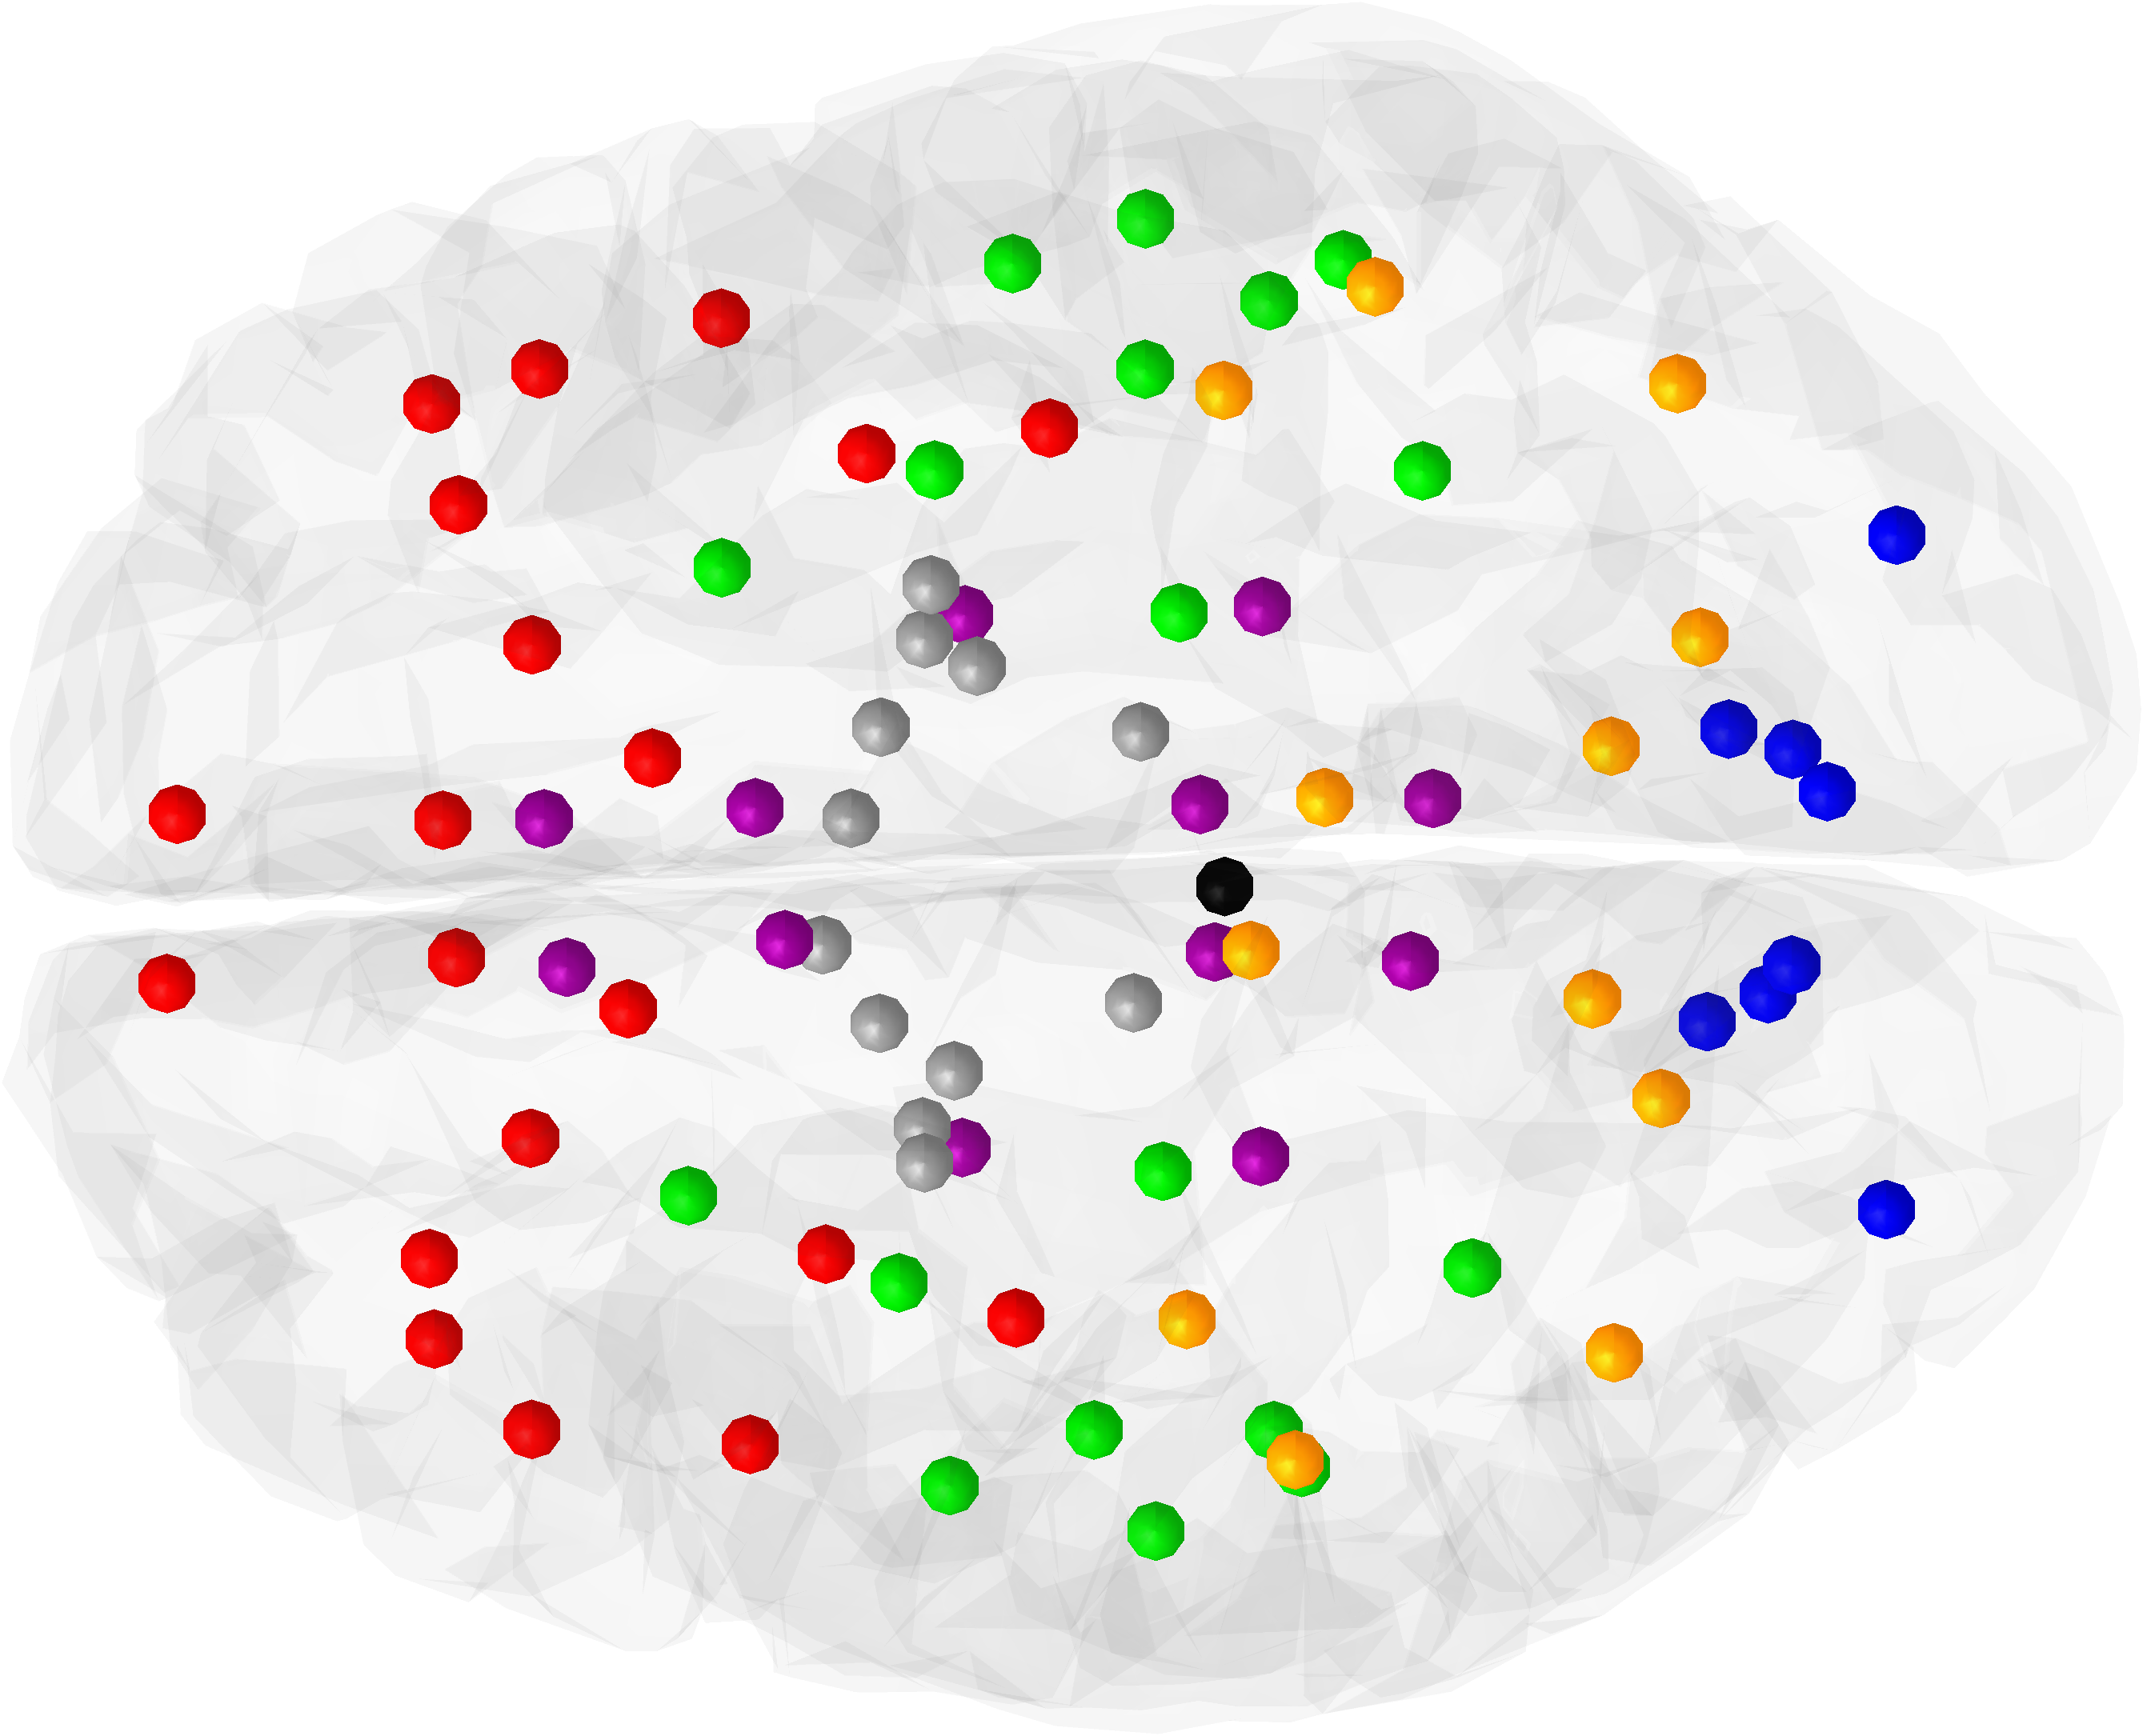
\includegraphics[width=\widthIm cm]
                        {../Figure/regioniCervelloAlto [Trasparente].png}};
                    \node[anchor=north west] at (FKR c2r2.north west)
                        {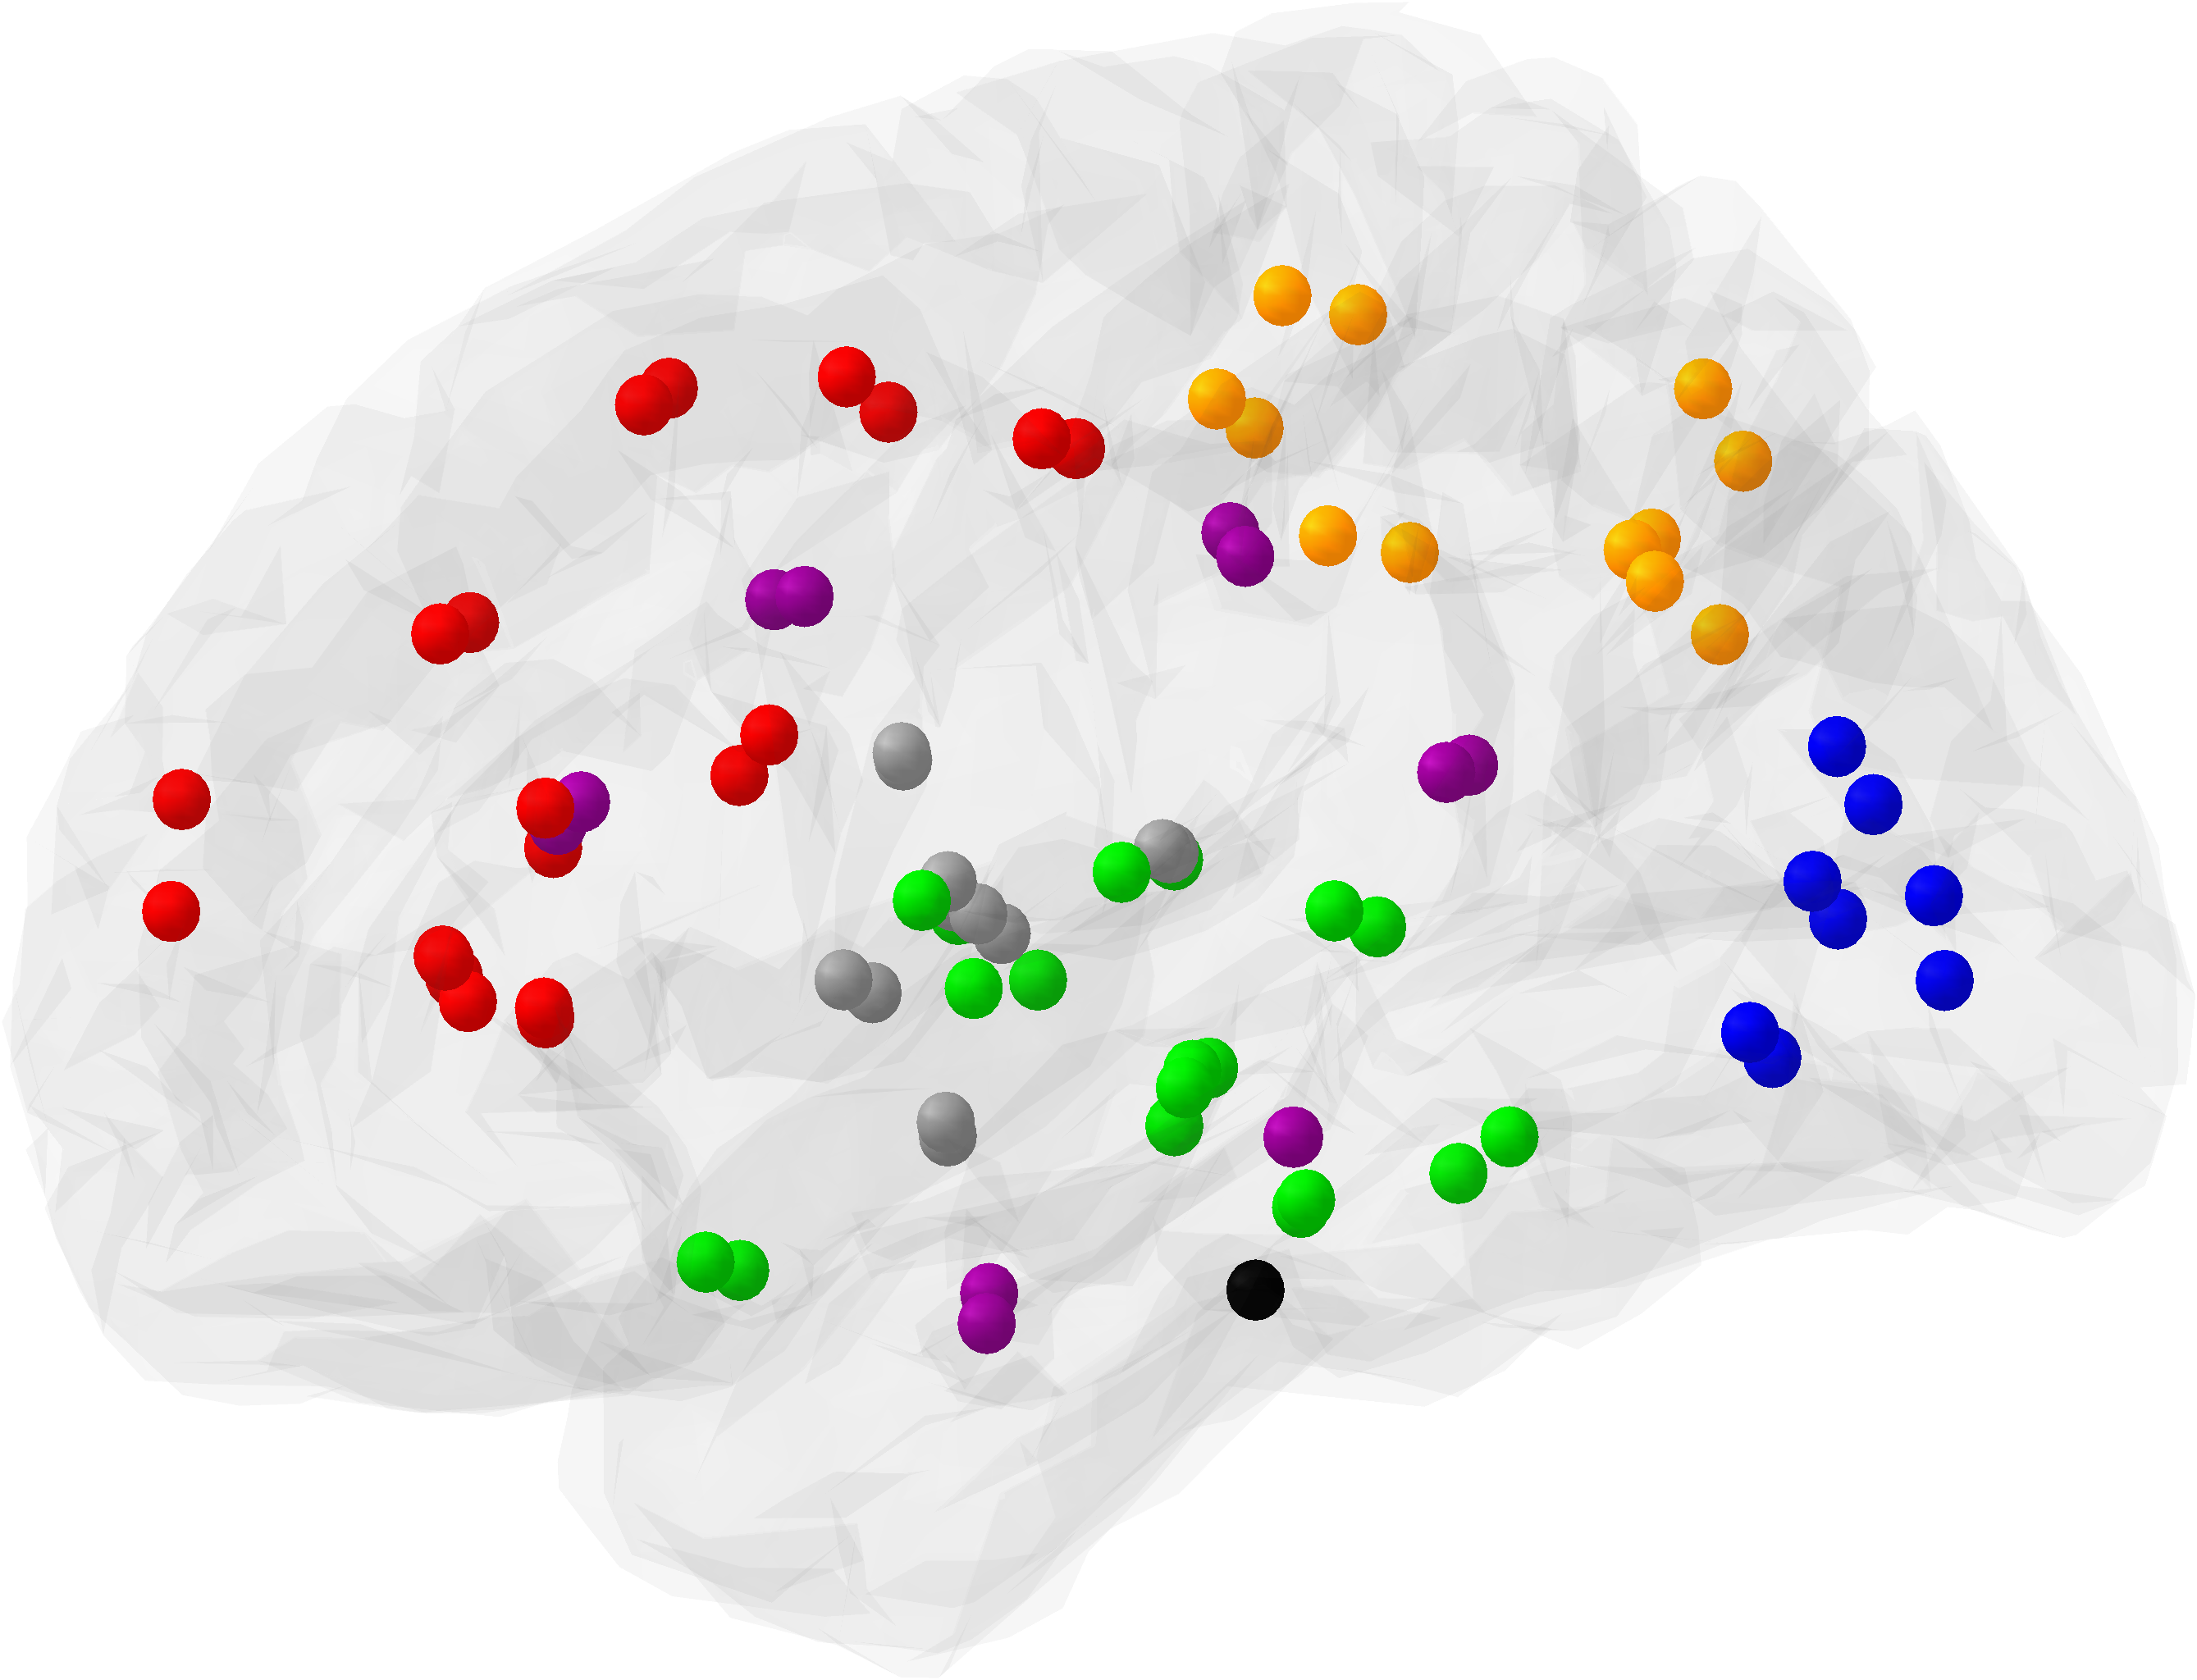
\includegraphics[width=\widthIm cm]
                        {../Figure/regioniCervelloLato [Trasparente].png}};
                    \newlength\heightIm
                    \settoheight{\heightIm}{
                        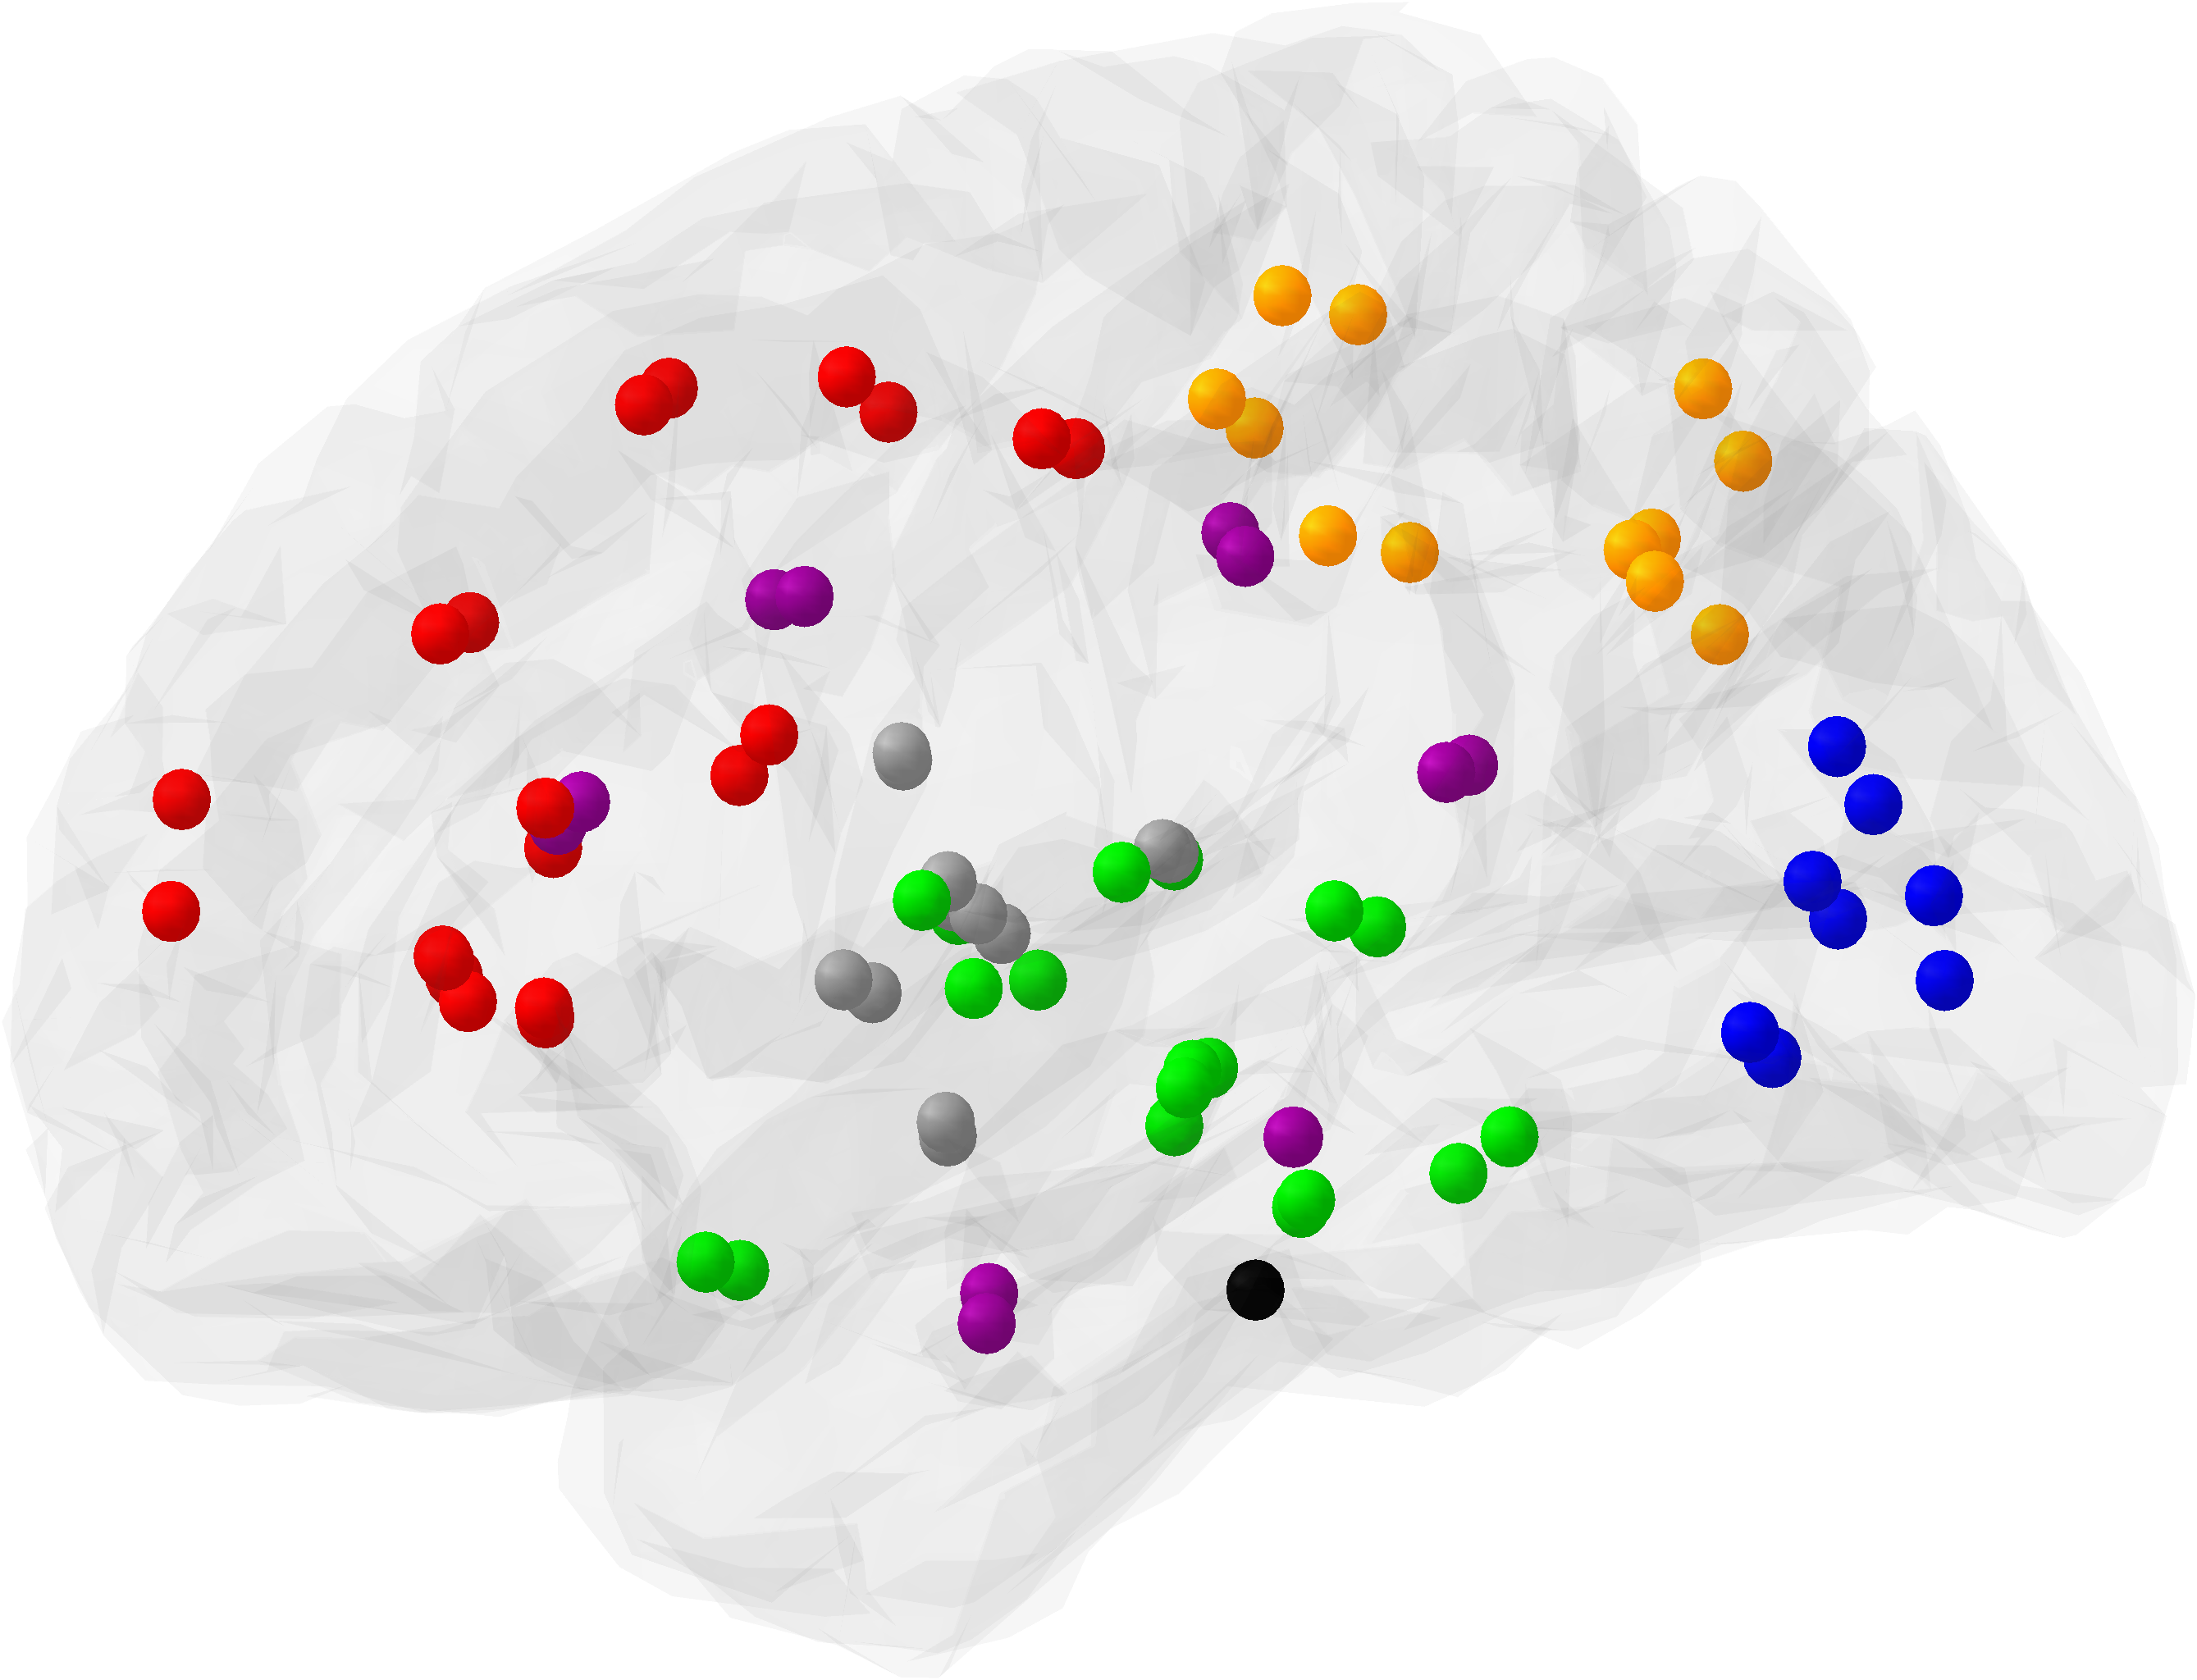
\includegraphics[width=\widthIm cm]
                        {../Figure/regioniCervelloLato [Trasparente].png}}
                    \node[anchor=north west] at (FKR c1r2.north west)
                        {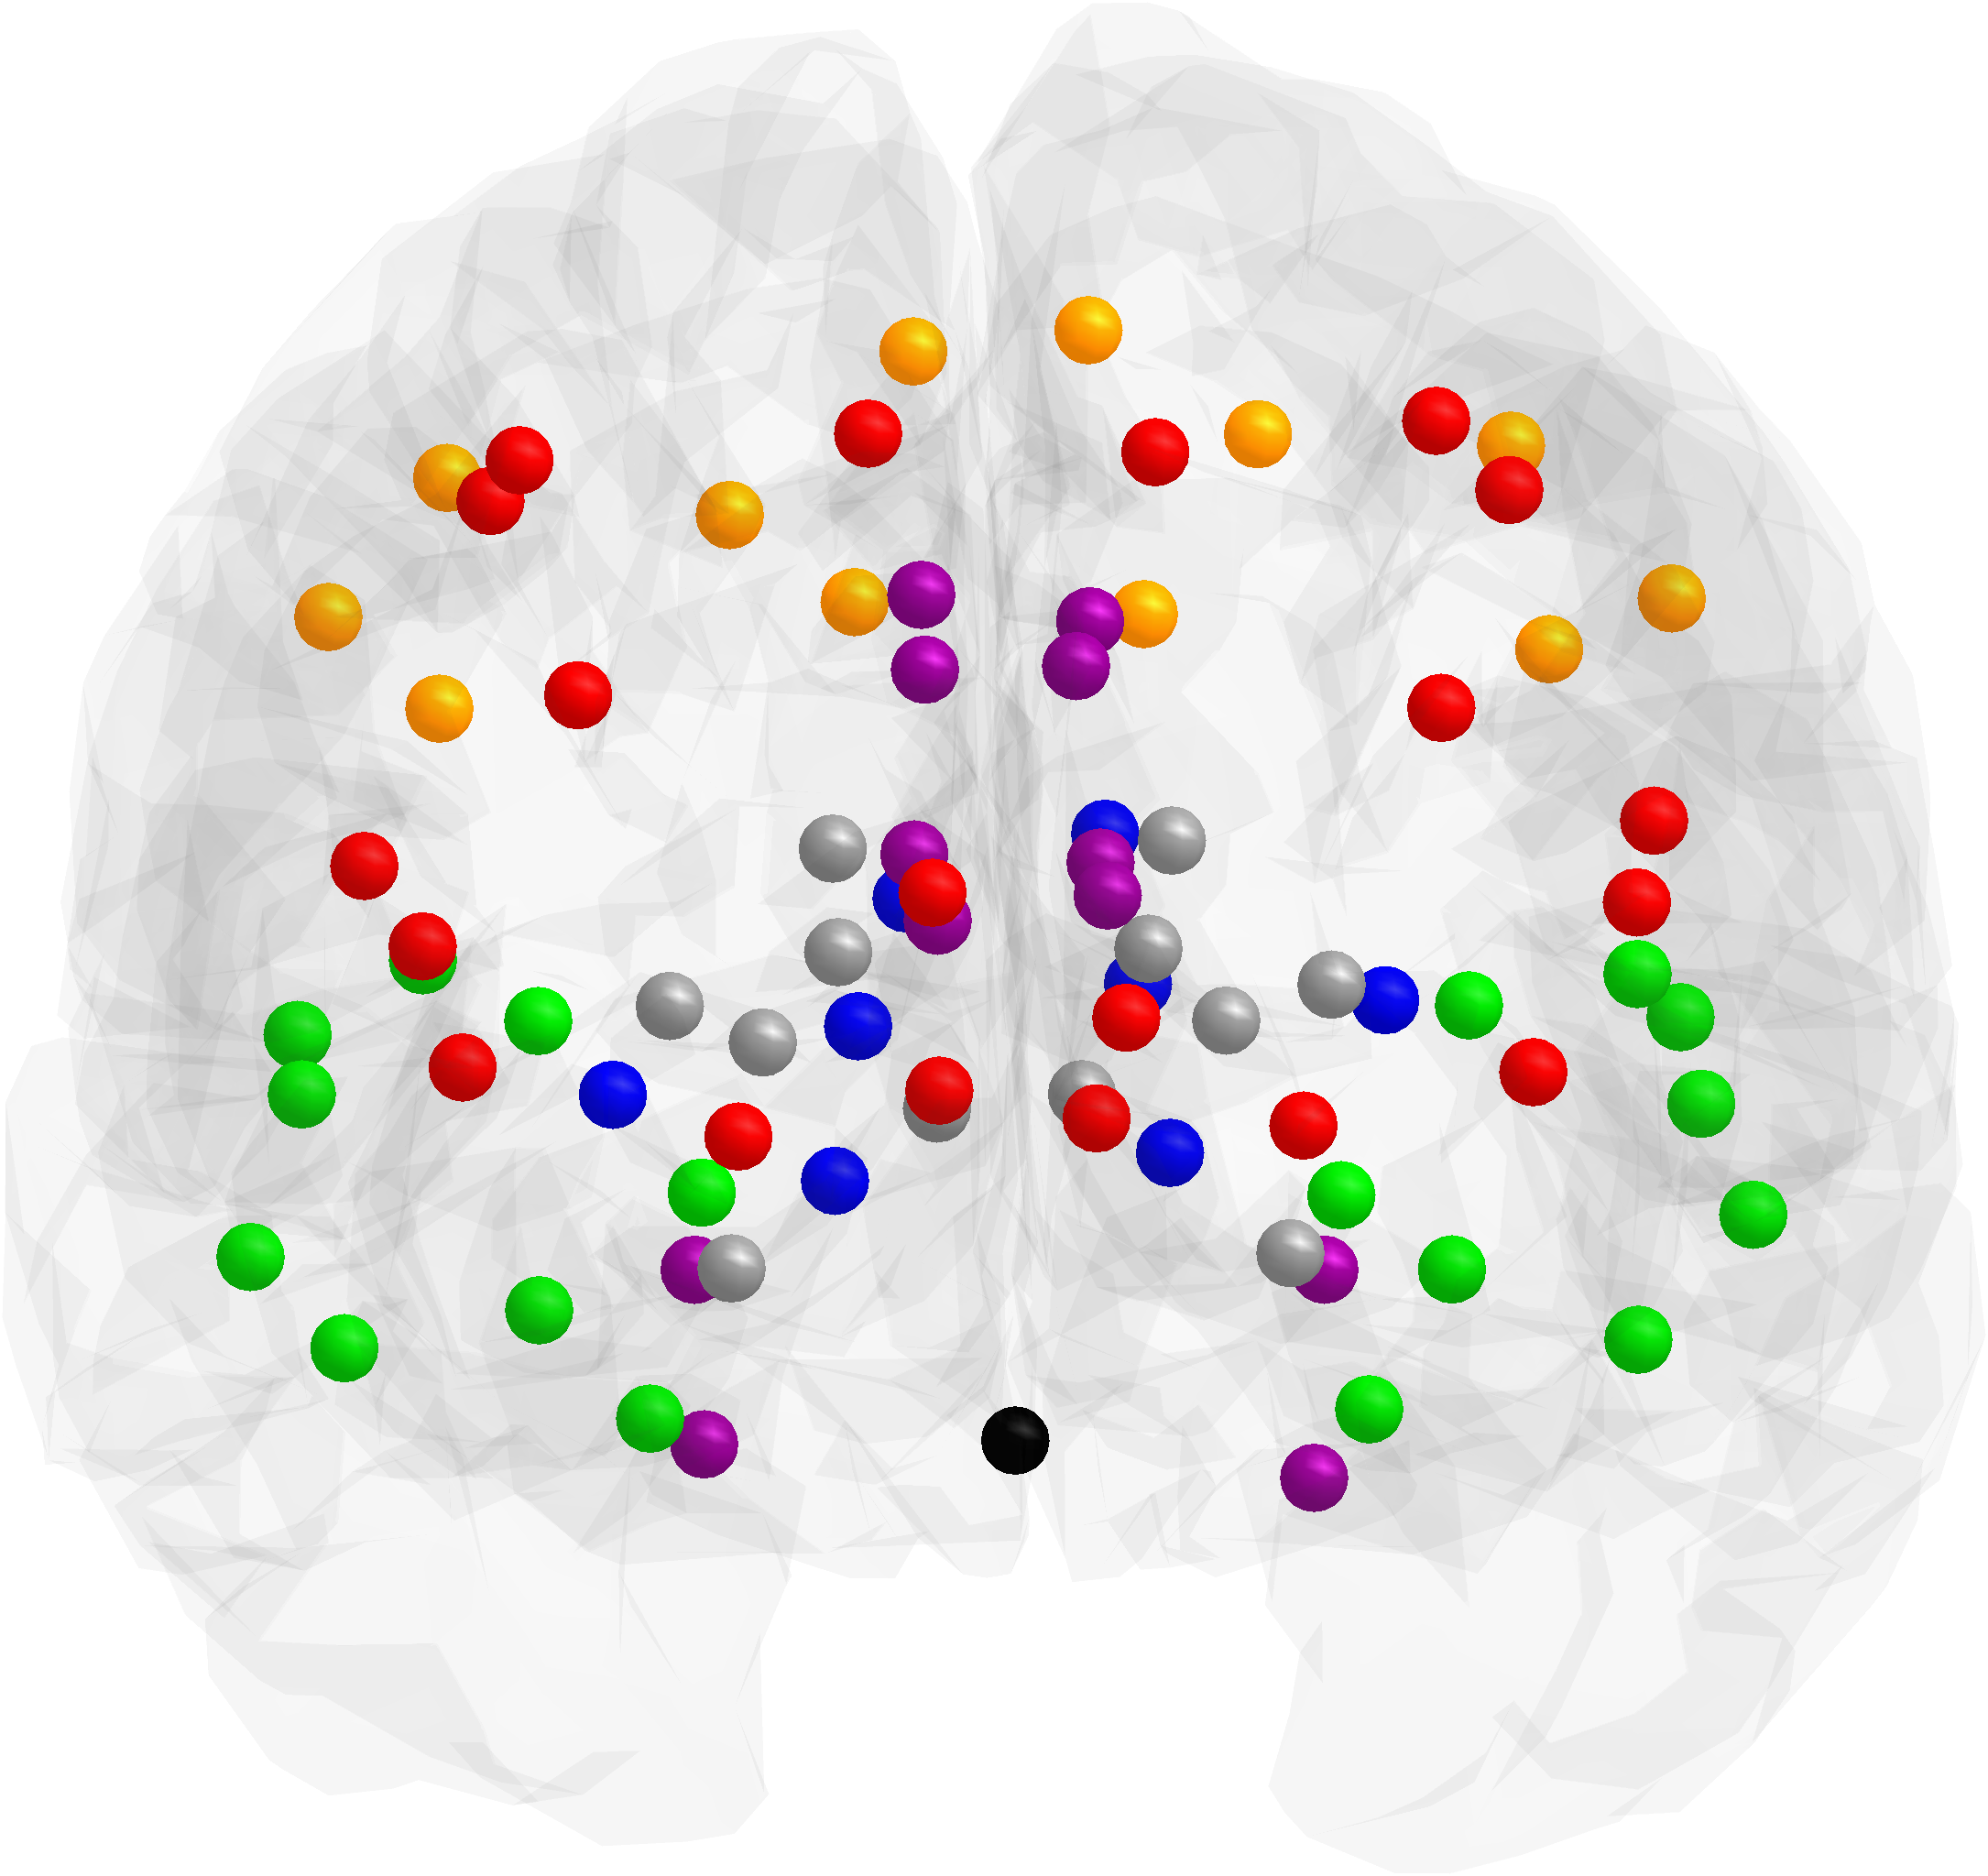
\includegraphics[height=\heightIm]
                        {../Figure/regioniCervelloFronte [Trasparente].png}};

                    % \pgfmathsetmacro\widthIm{3}
                    % \node[anchor=north west] at (FKR c2r1.north west)
                    %     {\includegraphics[width=\widthIm cm]
                    %     {../Figure/regioniCervelloFronte [Trasparente].png}};
                    %     % {../Figure/regioniCervelloFronte [Trasparente].png}};
                    % \node[anchor=north west] at (FKR c1r3.north west)
                    %     {\includegraphics[width=\widthIm cm]
                    %     {../Figure/regioniCervelloLato [Trasparente].png}};
                    %     % {../Figure/regioniCervelloLato [Trasparente].png}};
                    % \node[anchor=north west] at (FKR c1r4.north west)
                    %     {\includegraphics[width=\widthIm cm]
                    %     {../Figure/regioniCervelloAlto [Trasparente].png}};
                    %     % {../Figure/regioniCervelloAlto [Trasparente].png}};

                    %
                    \tikzset{SubCaption/.style={text width=4cm,anchor=south east,align=right}} %,inner sep=0pt,draw
                    \node[SubCaption] at (FKR c1r1.south east)
                        {\dimTesto{\captionSize}\sottoDidascalia{\selezionaLingua{$\mathbf L$ statica}{Static $\mathbf L$}\label{figFKStaticL}}};
                    \node[SubCaption] at (FKR c2r1.south east)
                        {\dimTesto{\captionSize}\sottoDidascalia{\selezionaLingua{$\mathbf L$ dinamica}{Dynamic $\mathbf L$}\label{figFKDynamicL}}};
                    \node[SubCaption] at (FKR c1r2.south east)
                        {\dimTesto{\captionSize}\sottoDidascalia{\selezionaLingua{Variante}{Variant} $f_d^l\leftrightarrow f_d^h$\label{figFKDynamicLVariant1}}};
                    \node[SubCaption] at (FKR c2r2.south east)
                        {\dimTesto{\captionSize}\sottoDidascalia{\selezionaLingua{Variante}{Variant} $f_d^l\leftrightarrow f_d^m$\label{figFKDynamicLVariant2}}};
                \end{tikzpicture}
            }}
            % }
            \caption{Confronti tra i gruppi.}
        \end{figure}
    \end{frame}

    \begin{frame}\frametitle{\insertsection{} - \insertsubsection{}}
        \begin{figure}[h!]
            \centering
            % \fbox{
            \makebox[\textwidth][c]{
            \resizebox{1.15\textwidth}{!}{
                \begin{tikzpicture}
                    \pgfmathsetmacro\heightPlot{(\heightPlot-\ySep)/2}

                    \pgfmathsetmacro\numMarker{10}
                    \pgfmathsetmacro\sizeMarker{2}

                    \pgfplotsset{
                        markOption/.style={
                            mark options={solid,magenta},
                            mark repeat=\numMarker,
                            mark size=\sizeMarker pt,
                            mark phase=\numMarker
                        }
                    }
                    \pgfplotsset{markX/.style={markOption,mark=x}}
                    \pgfplotsset{markO/.style={markOption,mark=o}}
                    \pgfplotsset{markT/.style={markOption,mark=triangle}}
                    \pgfplotsset{markD/.style={markOption,mark=diamond,}}
                    
                    \begin{groupplot}[
                        group style={
                            group name=FKN, % FK Nodi
                            group size=2 by 4,
                            horizontal sep=\xSep cm,
                            vertical sep=\ySep cm,
                            xlabels at=edge bottom,
                            ylabels at=edge left,
                            xticklabels at=edge bottom,
                            yticklabels at=edge left,
                            % x descriptions at=edge bottom
                        },
                        width=\widthPlot cm,
                        height=\heightPlot cm,
                        scale only axis,% Fondamentale per avere coerenza tra i due grafici,altrimenti non scalano correttamente
                        xmin=0,xmax=30,
                        xlabel={$t$ [\unit{\year}]},
                        xlabel style={
                            font=\color{white!15!black}\dimTesto{\labelSize},
                            yshift=.15cm,
                            % at={(ticklabel cs:1.0)},
                            % anchor=east,
                        },
                        ymin=0,ymax=1,
                        ylabel={$c$ [\%]},
                        ylabel style={
                            font=\color{white!15!black}\dimTesto{\labelSize},
                            yshift=-.15cm,
                            % at={(ticklabel cs:1.0)},
                            % anchor=east,
                        },
                        xticklabel style={
                            font=\dimTesto{\tickSize},
                            anchor=north
                        },
                        yticklabel style={
                            font=\dimTesto{\tickSize},
                            anchor=east,
                        },
                        ytick distance=0.2,
                        % ytick pos=right,
                        axis x line*=bottom,
                        axis y line*=left,
                        xmajorgrids,
                        ymajorgrids,
                        grid style={dashed},
                    ]
                        \nextgroupplot[
                            legend style={
                                legend cell align=left,
                                align=left,
                                legend pos=north west,
                                draw=white!15!black,
                                font=\dimTesto{\legendSize},
                                only marks,
                                % fill=none,
                                % draw=none,
                            },
                        ]
                        %\begingroup Rete
                        \addplot [color=black,dashed,line width=\lineWidth pt,markX]
                            table[row sep=crcr]{%
                        0	0.00240963855421687\\
                        0.4	0.00292466694502703\\
                        0.8	0.0035305179861389\\
                        1.2	0.00423575301794201\\
                        1.6	0.00504723498398097\\
                        2	0.00596943575665603\\
                        2.4	0.0070039357199673\\
                        2.8	0.00814928980826181\\
                        3.2	0.00940141280649762\\
                        3.6	0.0107545683067735\\
                        4	0.0122029430445418\\
                        4.4	0.0137426815454279\\
                        4.8	0.0153741809372719\\
                        5.2	0.0171044273807985\\
                        5.6	0.0189491963543618\\
                        6	0.0209350192977185\\
                        6.4	0.0231009077937645\\
                        6.8	0.0254998949309808\\
                        7.2	0.0282004848774309\\
                        7.6	0.0312880926644432\\
                        8	0.0348665130872463\\
                        8.4	0.0390593910331553\\
                        8.8	0.0440115859207475\\
                        9.2	0.0498902386293929\\
                        9.6	0.0568852662403692\\
                        10	0.0652089321886681\\
                        10.4	0.0750940704958346\\
                        10.8	0.0867904876309486\\
                        11.2	0.10055903446945\\
                        11.6	0.116662853917144\\
                        12	0.135355400497112\\
                        12.4	0.156865041896279\\
                        12.8	0.181376436304291\\
                        13.2	0.209009461483885\\
                        13.6	0.239797230657553\\
                        14	0.27366556384345\\
                        14.4	0.310416990722958\\
                        14.8	0.349722666286264\\
                        15.2	0.391125208620723\\
                        15.6	0.434054267034464\\
                        16	0.477854688437143\\
                        16.4	0.521824851855364\\
                        16.8	0.565260681983756\\
                        17.2	0.607499646096211\\
                        17.6	0.64795907033437\\
                        18	0.686164370104303\\
                        18.4	0.721764866878947\\
                        18.8	0.754537130164705\\
                        19.2	0.784377644312435\\
                        19.6	0.811287703587221\\
                        20	0.835353742069713\\
                        20.4	0.856725998020483\\
                        20.8	0.875597777061739\\
                        21.2	0.892186863129063\\
                        21.6	0.906719983868784\\
                        22	0.919420726658972\\
                        22.4	0.930500920517231\\
                        22.8	0.940155222609388\\
                        23.2	0.948558453341346\\
                        23.6	0.955865100622207\\
                        24	0.962210360830602\\
                        24.4	0.967712101522178\\
                        24.8	0.972473212388698\\
                        25.2	0.976583938997016\\
                        25.6	0.980123942011195\\
                        26	0.983163964488135\\
                        26.4	0.985767099239553\\
                        26.8	0.987989716732732\\
                        27.2	0.989882143197788\\
                        27.6	0.991489178331673\\
                        28	0.992850524801783\\
                        28.4	0.994001178674119\\
                        28.8	0.994971808297686\\
                        29.2	0.99578913267496\\
                        29.6	0.996476299730036\\
                        30	0.997053259343402\\
                        };
                        \addlegendentry{\selezionaLingua{$\mathbf L$ statica}{Static $\mathbf L$}}

                        \addplot [color=black,dashed,line width=\lineWidth pt,markO]
                            table[row sep=crcr]{%
                        0	0.00240963855421687\\
                        0.4	0.00292466694502704\\
                        0.8	0.00353037670879158\\
                        1.2	0.00423501803627785\\
                        1.6	0.00504486962177752\\
                        2	0.00596341503897998\\
                        2.4	0.00699069130203136\\
                        2.8	0.00812299766545468\\
                        3.2	0.00935313412456172\\
                        3.6	0.0106712672262949\\
                        4	0.0120664078520084\\
                        4.4	0.013528364491765\\
                        4.8	0.0150499472863316\\
                        5.2	0.0166291728604336\\
                        5.6	0.0182712625796095\\
                        6	0.0199903163475126\\
                        6.4	0.0218106457016816\\
                        6.8	0.0237678314840737\\
                        7.2	0.0259096139850376\\
                        7.6	0.0282967241716398\\
                        8	0.0310037317816587\\
                        8.4	0.0341199330334353\\
                        8.8	0.0377502408297489\\
                        9.2	0.0420159845340354\\
                        9.6	0.0470554822790771\\
                        10	0.0530242199689198\\
                        10.4	0.0600944561143297\\
                        10.8	0.0684540627005338\\
                        11.2	0.0783043969133344\\
                        11.6	0.0898569652481416\\
                        12	0.103328589913761\\
                        12.4	0.118934738495996\\
                        12.8	0.136880677176187\\
                        13.2	0.157350216107628\\
                        13.6	0.180492085973639\\
                        14	0.206404433689365\\
                        14.4	0.235118507677846\\
                        14.8	0.266583204847658\\
                        15.2	0.300652607133863\\
                        15.6	0.337078775099491\\
                        16	0.375511774084155\\
                        16.4	0.415508170995283\\
                        16.8	0.456548157501425\\
                        17.2	0.498060218007879\\
                        17.6	0.53945110208768\\
                        18	0.580138009244447\\
                        18.4	0.619579526677978\\
                        18.8	0.657302064498667\\
                        19.2	0.692919274370251\\
                        19.6	0.726143061529836\\
                        20	0.756786063801989\\
                        20.4	0.784756609835957\\
                        20.8	0.810047969789708\\
                        21.2	0.832724068666\\
                        21.6	0.852903760890441\\
                        22	0.870745377224232\\
                        22.4	0.88643271219622\\
                        22.8	0.900163076037351\\
                        23.2	0.912137598233439\\
                        23.6	0.922553687808428\\
                        24	0.931599421829736\\
                        24.4	0.939449608001268\\
                        24.8	0.946263297349167\\
                        25.2	0.952182561808558\\
                        25.6	0.957332367525031\\
                        26	0.961821357287403\\
                        26.4	0.965743314764949\\
                        26.8	0.969179042995374\\
                        27.2	0.972198375115821\\
                        27.6	0.974862060847082\\
                        28	0.977223335217604\\
                        28.4	0.979329061008235\\
                        28.8	0.98122042447923\\
                        29.2	0.982933240901932\\
                        29.6	0.984497985165164\\
                        30	0.985939700196658\\
                        };
                        \addlegendentry{\selezionaLingua{$\mathbf L$ dinamica}{Dynamic $\mathbf L$}}

                        \addplot [color=black,dashed,line width=\lineWidth pt,markT]
                            table[row sep=crcr]{%
                        0	0.00240963855421687\\
                        0.4	0.00292466694502704\\
                        0.8	0.00353046349226502\\
                        1.2	0.00423546449003536\\
                        1.6	0.00504629048463143\\
                        2	0.00596699177611491\\
                        2.4	0.00699847343070221\\
                        2.8	0.0081382795393668\\
                        3.2	0.00938089729500536\\
                        3.6	0.0107186727604209\\
                        4	0.0121433239859037\\
                        4.4	0.0136479242730715\\
                        4.8	0.0152291468033068\\
                        5.2	0.0168895389957385\\
                        5.6	0.0186396349312296\\
                        6	0.0204997972693338\\
                        6.4	0.0225017738468403\\
                        6.8	0.0246900281354168\\
                        7.2	0.0271229386729473\\
                        7.6	0.0298739565557521\\
                        8	0.0330327687272884\\
                        8.4	0.0367064496787836\\
                        8.8	0.0410205075685641\\
                        9.2	0.0461196539776193\\
                        9.6	0.0521680599080449\\
                        10	0.0593488138428377\\
                        10.4	0.0678622788868612\\
                        10.8	0.0779230599379738\\
                        11.2	0.0897553377226089\\
                        11.6	0.103586397728836\\
                        12	0.1196382689891\\
                        12.4	0.138117484001926\\
                        12.8	0.159203081449824\\
                        13.2	0.183033118349857\\
                        13.6	0.209690171414879\\
                        14	0.239186619227631\\
                        14.4	0.271450905819251\\
                        14.8	0.306316428124365\\
                        15.2	0.343515026126595\\
                        15.6	0.382677099480968\\
                        16	0.423339961473786\\
                        16.4	0.464965106875902\\
                        16.8	0.506963718165942\\
                        17.2	0.548728242647303\\
                        17.6	0.589666626400279\\
                        18	0.629235154917097\\
                        18.4	0.666966032072736\\
                        18.8	0.702486793406972\\
                        19.2	0.735530128892141\\
                        19.6	0.765934285008194\\
                        20	0.793635537249749\\
                        20.4	0.818655017361974\\
                        20.8	0.841082381980509\\
                        21.2	0.861058532112334\\
                        21.6	0.878759045744761\\
                        22	0.894379384467372\\
                        22.4	0.908122430491706\\
                        22.8	0.920188562623161\\
                        23.2	0.930768271829002\\
                        23.6	0.940037193791516\\
                        24	0.948153342602046\\
                        24.4	0.955256237495812\\
                        24.8	0.961467525318474\\
                        25.2	0.966892637900092\\
                        25.6	0.971623010779015\\
                        26	0.975738439182589\\
                        26.4	0.979309249577677\\
                        26.8	0.982398094537777\\
                        27.2	0.985061303926134\\
                        27.6	0.987349821898424\\
                        28	0.989309815831995\\
                        28.4	0.990983062124348\\
                        28.8	0.992407205377417\\
                        29.2	0.993615964649047\\
                        29.6	0.994639333998127\\
                        30	0.995503801313757\\
                        };
                        \addlegendentry{\selezionaLingua{Variante}{Variant} $f_d^l\leftrightarrow f_d^h$}

                        \addplot [color=black,dashed,line width=\lineWidth pt,markD]
                            table[row sep=crcr]{%
                        0	0.00240963855421687\\
                        0.4	0.00292466694502704\\
                        0.8	0.00353026489321835\\
                        1.2	0.00423444759451843\\
                        1.6	0.00504306804185975\\
                        2	0.005958912128902\\
                        2.4	0.00698095947118606\\
                        2.8	0.00810400883446393\\
                        3.2	0.0093188489973197\\
                        3.6	0.0106130799252713\\
                        4	0.0119725677525981\\
                        4.4	0.0133833858236493\\
                        4.8	0.014833998029241\\
                        5.2	0.0163174132053975\\
                        5.6	0.0178330860014076\\
                        6	0.0193884373308861\\
                        6.4	0.0209999780967762\\
                        6.8	0.0226941078857197\\
                        7.2	0.0245077051145078\\
                        7.6	0.0264886229404851\\
                        8	0.028696164098624\\
                        8.4	0.0312015403042915\\
                        8.8	0.0340882403747136\\
                        9.2	0.0374521469472745\\
                        9.6	0.0414011665828274\\
                        10	0.0460540881739466\\
                        10.4	0.0515383821148277\\
                        10.8	0.057986724163143\\
                        11.2	0.0655321961519918\\
                        11.6	0.074302384926898\\
                        12	0.084412938760297\\
                        12.4	0.0959614664586054\\
                        12.8	0.109022857269659\\
                        13.2	0.123647033963097\\
                        13.6	0.139859756417601\\
                        14	0.157666409927629\\
                        14.4	0.177057912225213\\
                        14.8	0.198017210408126\\
                        15.2	0.220524551919333\\
                        15.6	0.244559919656114\\
                        16	0.270101664905134\\
                        16.4	0.297121255934055\\
                        16.8	0.325574936357643\\
                        17.2	0.355393751178756\\
                        17.6	0.386473740068834\\
                        18	0.418668100359564\\
                        18.4	0.451782832104795\\
                        18.8	0.485576872474803\\
                        19.2	0.519767099241957\\
                        19.6	0.554037928390108\\
                        20	0.588054635434282\\
                        20.4	0.621479062523825\\
                        20.8	0.653986084032703\\
                        21.2	0.685279127616549\\
                        21.6	0.71510320475342\\
                        22	0.743254283246468\\
                        22.4	0.769584376249619\\
                        22.8	0.794002324398698\\
                        23.2	0.816470786459096\\
                        23.6	0.837000327848781\\
                        24	0.855641656747828\\
                        24.4	0.872477016418602\\
                        24.8	0.887611558914315\\
                        25.2	0.901165280833763\\
                        25.6	0.913265872748781\\
                        26	0.924042669027765\\
                        26.4	0.933621792470381\\
                        26.8	0.942122541919244\\
                        27.2	0.949655030292379\\
                        27.6	0.95631901617339\\
                        28	0.962203782030172\\
                        28.4	0.967388819402564\\
                        28.8	0.971945018902633\\
                        29.2	0.975936054509248\\
                        29.6	0.979419700531671\\
                        30	0.982448908214976\\
                        };
                        \addlegendentry{\selezionaLingua{Variante}{Variant} $f_d^l\leftrightarrow f_d^m$}
                        %\endgroup
                        
                        \nextgroupplot
                        %\begingroup Temporale
                        \addplot [color=mycolor1,line width=\lineWidth pt,markX]
                            table[row sep=crcr]{%
                        0	0\\
                        0.4	7.04171308036035e-05\\
                        0.8	0.0001672048701582\\
                        1.2	0.000297593640187364\\
                        1.6	0.00047039001380224\\
                        2	0.000696245355283955\\
                        2.4	0.000987971062312688\\
                        2.8	0.00136091844256661\\
                        3.2	0.00183344759533614\\
                        3.6	0.00242751517133344\\
                        4	0.00316941440823133\\
                        4.4	0.00409070162785883\\
                        4.8	0.0052293412150801\\
                        5.2	0.00663109608624231\\
                        5.6	0.00835118270409559\\
                        6	0.0104561978995357\\
                        6.4	0.0130263069503838\\
                        6.8	0.0161576549879967\\
                        7.2	0.0199649221440234\\
                        7.6	0.0245838816769949\\
                        8	0.0301737350345084\\
                        8.4	0.0369188864319131\\
                        8.8	0.0450296858238938\\
                        9.2	0.0547415269701936\\
                        9.6	0.0663115655831579\\
                        10	0.0800122689302831\\
                        10.4	0.0961210876435254\\
                        10.8	0.114905823369919\\
                        11.2	0.136605802613332\\
                        11.6	0.161409749715729\\
                        12	0.189432177122574\\
                        12.4	0.220690968895706\\
                        12.8	0.255089347296453\\
                        13.2	0.292405334188646\\
                        13.6	0.332291046145129\\
                        14	0.374282810570177\\
                        14.4	0.417821474873627\\
                        14.8	0.462280801846695\\
                        15.2	0.507000837509718\\
                        15.6	0.551322761367464\\
                        16	0.594621937569825\\
                        16.4	0.636336489351372\\
                        16.8	0.67598949571434\\
                        17.2	0.7132037021458\\
                        17.6	0.747708388245802\\
                        18	0.779338741329222\\
                        18.4	0.808028728214549\\
                        18.8	0.833798971665503\\
                        19.2	0.856741436625102\\
                        19.6	0.877002761950399\\
                        20	0.894767852409514\\
                        20.4	0.910244952625648\\
                        20.8	0.923652965638926\\
                        21.2	0.935211348637565\\
                        21.6	0.945132577492984\\
                        22	0.953616942421088\\
                        22.4	0.960849312865095\\
                        22.8	0.966997468289305\\
                        23.2	0.972211606252168\\
                        23.6	0.976624685770624\\
                        24	0.980353324228943\\
                        24.4	0.983499027729118\\
                        24.8	0.986149590853747\\
                        25.2	0.988380549116205\\
                        25.6	0.990256605153319\\
                        26	0.991832978589689\\
                        26.4	0.993156650736052\\
                        26.8	0.994267490329683\\
                        27.2	0.995199256770151\\
                        27.6	0.995980483956098\\
                        28	0.996635251872115\\
                        28.4	0.9971838552805\\
                        28.8	0.997643379824352\\
                        29.2	0.998028195975112\\
                        29.6	0.998350380868087\\
                        30	0.998620077379581\\
                        };
                        % \addlegendentry{\selezionaLingua{Temporale}{Temporal}}

                        \addplot [color=mycolor1,line width=\lineWidth pt,markO]
                            table[row sep=crcr]{%
                        0	0\\
                        0.4	7.04171308036133e-05\\
                        0.8	0.000160204478730234\\
                        1.2	0.000274229751227403\\
                        1.6	0.00041838107007992\\
                        2	0.000599771146948772\\
                        2.4	0.000826985818206162\\
                        2.8	0.00111039086316631\\
                        3.2	0.00146251417226236\\
                        3.6	0.00189852303205726\\
                        4	0.00243681822712462\\
                        4.4	0.0030997677052262\\
                        4.8	0.00391460276276395\\
                        5.2	0.0049144991126796\\
                        5.6	0.00613986352225551\\
                        6	0.00763984310680477\\
                        6.4	0.00947406724922501\\
                        6.8	0.0117146191088141\\
                        7.2	0.0144482116800851\\
                        7.6	0.0177785087049756\\
                        8	0.0218284796003422\\
                        8.4	0.0267426067031272\\
                        8.8	0.0326886713040044\\
                        9.2	0.0398587350616237\\
                        9.6	0.0484688155709467\\
                        10	0.0587566497176559\\
                        10.4	0.0709768795087045\\
                        10.8	0.0853930280250344\\
                        11.2	0.102265809186112\\
                        11.6	0.121837675999235\\
                        12	0.144314068043564\\
                        12.4	0.16984252466544\\
                        12.8	0.19849157099979\\
                        13.2	0.23023188555407\\
                        13.6	0.264922527830761\\
                        14	0.302304791355348\\
                        14.4	0.342005499594211\\
                        14.8	0.383550355568915\\
                        15.2	0.426386487991631\\
                        15.6	0.469911893314772\\
                        16	0.513508376927369\\
                        16.4	0.556574131419159\\
                        16.8	0.598552401166547\\
                        17.2	0.638953692827227\\
                        17.6	0.677370391185569\\
                        18	0.713483994678844\\
                        18.4	0.747066121817909\\
                        18.8	0.777974805250985\\
                        19.2	0.806147485508821\\
                        19.6	0.831591792853709\\
                        20	0.854374903888285\\
                        20.4	0.874612097511601\\
                        20.8	0.89245509676038\\
                        21.2	0.908080783620345\\
                        21.6	0.921680834273205\\
                        22	0.933452711425259\\
                        22.4	0.94359228451148\\
                        22.8	0.952288167008613\\
                        23.2	0.959717700773094\\
                        23.6	0.966044403105609\\
                        24	0.971416628952578\\
                        24.4	0.975967181781242\\
                        24.8	0.979813619876049\\
                        25.2	0.983059037060147\\
                        25.6	0.985793137333963\\
                        26	0.988093464064791\\
                        26.4	0.990026681654189\\
                        26.8	0.991649838940975\\
                        27.2	0.99301156845475\\
                        27.6	0.994153194441266\\
                        28	0.995109736205768\\
                        28.4	0.995910802767694\\
                        28.8	0.996581381050122\\
                        29.2	0.9971425236734\\
                        29.6	0.997611944562676\\
                        30	0.998004531541114\\
                        };
                        %\addlegendentry{Temporal}

                        \addplot [color=mycolor1,line width=\lineWidth pt,markT]
                            table[row sep=crcr]{%
                        0	0\\
                        0.4	7.04171308036133e-05\\
                        0.8	0.000165166156409918\\
                        1.2	0.000290851380546929\\
                        1.6	0.000455512345184376\\
                        2	0.000668889176693133\\
                        2.4	0.000942741128352748\\
                        2.8	0.00129123697248231\\
                        3.2	0.00173144109237988\\
                        3.6	0.00228392346531872\\
                        4	0.00297352443472908\\
                        4.4	0.00383030582799967\\
                        4.8	0.00489071856074137\\
                        5.2	0.00619901346036018\\
                        5.6	0.00780891632894931\\
                        6	0.00978557902577754\\
                        6.4	0.0122078031061734\\
                        6.8	0.0151705074827281\\
                        7.2	0.018787371672288\\
                        7.6	0.0231935257355591\\
                        8	0.0285480715089564\\
                        8.4	0.0350361036791183\\
                        8.8	0.0428697552532974\\
                        9.2	0.0522876314077549\\
                        9.6	0.0635518457372808\\
                        10	0.0769417823189689\\
                        10.4	0.0927437477081728\\
                        10.8	0.111235935713941\\
                        11.2	0.132668680659229\\
                        11.6	0.157240842849424\\
                        12	0.185074265491333\\
                        12.4	0.216189333826515\\
                        12.8	0.250485402059289\\
                        13.2	0.28772986391088\\
                        13.6	0.327558713913822\\
                        14	0.369489668815964\\
                        14.4	0.412946716986107\\
                        14.8	0.457292961800427\\
                        15.2	0.501867392500477\\
                        15.6	0.546021037140453\\
                        16	0.589148734209148\\
                        16.4	0.630714115813389\\
                        16.8	0.670266840205603\\
                        17.2	0.707452260043153\\
                        17.6	0.742014396418928\\
                        18	0.773793354822625\\
                        18.4	0.802718338748243\\
                        18.8	0.828797363310813\\
                        19.2	0.852104738423687\\
                        19.6	0.872767378915955\\
                        20	0.89095095679362\\
                        20.4	0.906846793328707\\
                        20.8	0.920660188322803\\
                        21.2	0.932600631070063\\
                        21.6	0.942874079729357\\
                        22	0.951677275370415\\
                        22.4	0.959193898375128\\
                        22.8	0.965592283203566\\
                        23.2	0.971024373838635\\
                        23.6	0.975625610841277\\
                        24	0.979515475445674\\
                        24.4	0.982798462762692\\
                        24.8	0.985565305142832\\
                        25.2	0.987894312095757\\
                        25.6	0.989852731890377\\
                        26	0.991498071142368\\
                        26.4	0.992879332644037\\
                        26.8	0.994038149330916\\
                        27.2	0.995009804758143\\
                        27.6	0.995824138910521\\
                        28	0.996506343595703\\
                        28.4	0.997077654898535\\
                        28.8	0.997555951859063\\
                        29.2	0.997956271172666\\
                        29.6	0.998291247663961\\
                        30	0.998571489818344\\
                        };
                        %\addlegendentry{Temporal}
                        
                        \addplot [color=mycolor1,line width=\lineWidth pt,markD]
                            table[row sep=crcr]{%
                        0	0\\
                        0.4	7.04171308036133e-05\\
                        0.8	0.000157749107881152\\
                        1.2	0.000267151437266578\\
                        1.6	0.000404786386885858\\
                        2	0.00057813248222222\\
                        2.4	0.000796340761190278\\
                        2.8	0.0010706617865807\\
                        3.2	0.00141496732225662\\
                        3.6	0.00184639206742639\\
                        4	0.00238612299840047\\
                        4.4	0.00306036616762194\\
                        4.8	0.00390152279883559\\
                        5.2	0.00494960751290817\\
                        5.6	0.00625394033220117\\
                        6	0.00787513878654531\\
                        6.4	0.00988742402568133\\
                        6.8	0.0123812311866352\\
                        7.2	0.0154660739403725\\
                        7.6	0.019273549598455\\
                        8	0.02396027744663\\
                        8.4	0.0297104335021204\\
                        8.8	0.0367373788294063\\
                        9.2	0.0452836853024394\\
                        9.6	0.0556186693981976\\
                        10	0.0680324040244606\\
                        10.4	0.0828251733747851\\
                        10.8	0.100291573379644\\
                        11.2	0.120699047024776\\
                        11.6	0.144261636834894\\
                        12	0.171111076359712\\
                        12.4	0.201268789795052\\
                        12.8	0.234623495065142\\
                        13.2	0.270919380225084\\
                        13.6	0.309758817009664\\
                        14	0.350621219830394\\
                        14.4	0.392896418130325\\
                        14.8	0.435927720748344\\
                        15.2	0.479057780381828\\
                        15.6	0.521670136036593\\
                        16	0.563220947452894\\
                        16.4	0.603258257290301\\
                        16.8	0.641429074816672\\
                        17.2	0.677476736256751\\
                        17.6	0.71123191340735\\
                        18	0.742600430196937\\
                        18.4	0.771550196176724\\
                        18.8	0.798098624099987\\
                        19.2	0.822301217624899\\
                        19.6	0.844241665778649\\
                        20	0.864023634757299\\
                        20.4	0.881764334478245\\
                        20.8	0.897589769463849\\
                        21.2	0.911631386728708\\
                        21.6	0.924023692072642\\
                        22	0.934902385626632\\
                        22.4	0.944402668544242\\
                        22.8	0.952657540511153\\
                        23.2	0.95979607116919\\
                        23.6	0.965941737318616\\
                        24	0.971210956819797\\
                        24.4	0.975711932835026\\
                        24.8	0.979543874229075\\
                        25.2	0.982796603939399\\
                        25.6	0.985550522792126\\
                        26	0.987876868165527\\
                        26.4	0.989838194918575\\
                        26.8	0.99148900643893\\
                        27.2	0.992876471914162\\
                        27.6	0.994041177925264\\
                        28	0.995017875257365\\
                        28.4	0.995836193620725\\
                        28.8	0.996521306893831\\
                        29.2	0.997094539281931\\
                        29.6	0.99757390853901\\
                        30	0.997974606418337\\
                        };
                        %\addlegendentry{Temporal}
                        %\endgroup
                        
                        \nextgroupplot
                        %\begingroup Frontale
                        \addplot [color=black!20!red,line width=\lineWidth pt,markX]
                            table[row sep=crcr]{%
                        0	0\\
                        0.4	7.45220646300236e-07\\
                        0.8	2.66053818596183e-06\\
                        1.2	6.33256066900219e-06\\
                        1.6	1.25599498691122e-05\\
                        2	2.24173470551563e-05\\
                        2.4	3.73363879315031e-05\\
                        2.8	5.92082605309682e-05\\
                        3.2	9.0513507711793e-05\\
                        3.6	0.000134486352877914\\
                        4	0.000195322780129838\\
                        4.4	0.000278443973293844\\
                        4.8	0.000390829557993377\\
                        5.2	0.000541438442021968\\
                        5.6	0.000741738944577451\\
                        6	0.00100637433954323\\
                        6.4	0.00135399482479046\\
                        6.8	0.00180829203008117\\
                        7.2	0.00239927699995348\\
                        7.6	0.00316484624780737\\
                        8	0.00415268148980219\\
                        8.4	0.00542252468862067\\
                        8.8	0.00704885754264351\\
                        9.2	0.00912398850054889\\
                        9.6	0.0117615039533295\\
                        10	0.0150999649500406\\
                        10.4	0.0193066172028745\\
                        10.8	0.0245807221693896\\
                        11.2	0.0311559081354635\\
                        11.6	0.039300692918927\\
                        12	0.049316077679901\\
                        12.4	0.0615289222557084\\
                        12.8	0.0762797949966285\\
                        13.2	0.0939042850401585\\
                        13.6	0.114707509671452\\
                        14	0.138932808211049\\
                        14.4	0.166727286534176\\
                        14.8	0.198108626659432\\
                        15.2	0.232938846196642\\
                        15.6	0.270910855937973\\
                        16	0.311552298422199\\
                        16.4	0.35424831525503\\
                        16.8	0.398281235287812\\
                        17.2	0.442881758740523\\
                        17.6	0.487284085238452\\
                        18	0.530777186562522\\
                        18.4	0.572745950288165\\
                        18.8	0.61269852121596\\
                        19.2	0.650278930262996\\
                        19.6	0.685266305410928\\
                        20	0.717563301992899\\
                        20.4	0.747176945499526\\
                        20.8	0.7741951081684\\
                        21.2	0.798761585881849\\
                        21.6	0.821052339375135\\
                        22	0.841254948589519\\
                        22.4	0.859552699220945\\
                        22.8	0.876113995913308\\
                        23.2	0.891087044725842\\
                        23.6	0.904599073640304\\
                        24	0.916758874154351\\
                        24.4	0.927661227030982\\
                        24.8	0.937391838416012\\
                        25.2	0.946031708062134\\
                        25.6	0.953660276501559\\
                        26	0.960357132826855\\
                        26.4	0.966202411347959\\
                        26.8	0.971276213282269\\
                        27.2	0.975657458641542\\
                        27.6	0.979422538204022\\
                        28	0.982644043066933\\
                        28.4	0.985389741598044\\
                        28.8	0.98772187833009\\
                        29.2	0.989696799294941\\
                        29.6	0.991364865235348\\
                        30	0.992770593646474\\
                        };
                        % \addlegendentry{\selezionaLingua{Frontale}{Frontal}}

                        \addplot [color=black!20!red,line width=\lineWidth pt,markO]
                            table[row sep=crcr]{%
                        0	0\\
                        0.4	7.45220646300334e-07\\
                        0.8	2.50679278954728e-06\\
                        1.2	5.65142289330294e-06\\
                        1.6	1.06678866297409e-05\\
                        2	1.82009662273744e-05\\
                        2.4	2.90947218676351e-05\\
                        2.8	4.44475154788143e-05\\
                        3.2	6.56818596222808e-05\\
                        3.6	9.46329718363549e-05\\
                        4	0.000133660906452178\\
                        4.4	0.000185792347093542\\
                        4.8	0.000254899614780255\\
                        5.2	0.000345926223822681\\
                        5.6	0.000465170445608714\\
                        6	0.000620640856273798\\
                        6.4	0.000822500764773039\\
                        6.8	0.00108362171881381\\
                        7.2	0.00142026987133137\\
                        7.6	0.0018529526450829\\
                        8	0.00240745645613401\\
                        8.4	0.00311610856377635\\
                        8.8	0.00401929630607221\\
                        9.2	0.00516727337835825\\
                        9.6	0.0066222729679803\\
                        10	0.00846092807169094\\
                        10.4	0.0107769657440445\\
                        10.8	0.0136840889953019\\
                        11.2	0.0173188819141756\\
                        11.6	0.0218434658074856\\
                        12	0.0274474960007322\\
                        12.4	0.0343489276912153\\
                        12.8	0.0427928156033585\\
                        13.2	0.0530472857978012\\
                        13.6	0.0653957898058071\\
                        14	0.0801248983356336\\
                        14.4	0.0975072891827826\\
                        14.8	0.11778027214227\\
                        15.2	0.141121137474421\\
                        15.6	0.167621670467483\\
                        16	0.197265091574782\\
                        16.4	0.2299091519048\\
                        16.8	0.265278872896257\\
                        17.2	0.30297135857833\\
                        17.6	0.342473352781343\\
                        18	0.383190114575283\\
                        18.4	0.42448223395656\\
                        18.8	0.465705689614116\\
                        19.2	0.506250086750563\\
                        19.6	0.545570670592956\\
                        20	0.583211175790366\\
                        20.4	0.61881642032666\\
                        20.8	0.652135294092607\\
                        21.2	0.683016027896279\\
                        21.6	0.711396168583539\\
                        22	0.73728957954041\\
                        22.4	0.760772261671418\\
                        22.8	0.781968139811095\\
                        23.2	0.801035424335798\\
                        23.6	0.818153859110557\\
                        24	0.833513101063604\\
                        24.4	0.847302553757251\\
                        24.8	0.859703075293808\\
                        25.2	0.870880991393284\\
                        25.6	0.880984704698206\\
                        26	0.890143903264043\\
                        26.4	0.898471003544139\\
                        26.8	0.906064127875191\\
                        27.2	0.913010721898124\\
                        27.6	0.919390920612136\\
                        28	0.925279958012448\\
                        28.4	0.930749215188949\\
                        28.8	0.935865831732462\\
                        29.2	0.940691101945817\\
                        29.6	0.945278107652467\\
                        30	0.949669187819695\\
                        };
                        %\addlegendentry{Frontal}

                        \addplot [color=black!20!red,line width=\lineWidth pt,markT]
                            table[row sep=crcr]{%
                        0	0\\
                        0.4	7.45220646300334e-07\\
                        0.8	2.56318233821684e-06\\
                        1.2	5.89934817277606e-06\\
                        1.6	1.13502763466143e-05\\
                        2	1.97060166819355e-05\\
                        2.4	3.20039995684702e-05\\
                        2.8	4.95973653180441e-05\\
                        3.2	7.42415309180588e-05\\
                        3.6	0.000108203828025785\\
                        4	0.000154402306783394\\
                        4.4	0.000216581323794741\\
                        4.8	0.00029953336500901\\
                        5.2	0.000409378746919266\\
                        5.6	0.000553917444091609\\
                        6	0.00074307034679737\\
                        6.4	0.00098943076570679\\
                        6.8	0.00130895091380414\\
                        7.2	0.00172179224217078\\
                        7.6	0.00225337254270601\\
                        8	0.00293564603954958\\
                        8.4	0.00380865424274561\\
                        8.8	0.00492238350851836\\
                        9.2	0.00633895759414814\\
                        9.6	0.00813517649433983\\
                        10	0.0104053817032985\\
                        10.4	0.0132645766543602\\
                        10.8	0.0168516524170231\\
                        11.2	0.0213324560381939\\
                        11.6	0.0269022883119393\\
                        12	0.0337872326975667\\
                        12.4	0.0422435149734787\\
                        12.8	0.0525539132620895\\
                        13.2	0.0650201477589541\\
                        13.6	0.0799502737277195\\
                        14	0.0976404865892006\\
                        14.4	0.11835150520799\\
                        14.8	0.142280827225554\\
                        15.2	0.169533505348751\\
                        15.6	0.200095364416471\\
                        16	0.233813331100114\\
                        16.4	0.270387356653469\\
                        16.8	0.309377054001637\\
                        17.2	0.350223781625125\\
                        17.6	0.392286023694096\\
                        18	0.43488332705131\\
                        18.4	0.477342517966777\\
                        18.8	0.519039863889315\\
                        19.2	0.559434201010175\\
                        19.6	0.598088298594823\\
                        20	0.634678131847057\\
                        20.4	0.668991618045676\\
                        20.8	0.700919377682572\\
                        21.2	0.730440239202238\\
                        21.6	0.757603820490692\\
                        22	0.782511980050284\\
                        22.4	0.805300514093623\\
                        22.8	0.826122262264286\\
                        23.2	0.845132683564204\\
                        23.6	0.862478815740608\\
                        24	0.878292216825793\\
                        24.4	0.892685994423021\\
                        24.8	0.905755454069944\\
                        25.2	0.917581399583077\\
                        25.6	0.928234838832776\\
                        26	0.937781855660231\\
                        26.4	0.946287671852877\\
                        26.8	0.953819334667686\\
                        27.2	0.960446891804643\\
                        27.6	0.966243249463038\\
                        28	0.971283098170749\\
                        28.4	0.975641339173669\\
                        28.8	0.979391390634248\\
                        29.2	0.982603647668567\\
                        29.6	0.985344255554799\\
                        30	0.98767425775702\\
                        };
                        %\addlegendentry{Frontal}

                        \addplot [color=black!20!red,line width=\lineWidth pt,markD]
                            table[row sep=crcr]{%
                        0	0\\
                        0.4	7.45220646300334e-07\\
                        0.8	2.31709465233067e-06\\
                        1.2	4.8512564918643e-06\\
                        1.6	8.54316936520972e-06\\
                        2	1.36577430275517e-05\\
                        2.4	2.05431902871435e-05\\
                        2.8	2.96496350569145e-05\\
                        3.2	4.15532830965348e-05\\
                        3.6	5.69872910963718e-05\\
                        4	7.68808345836021e-05\\
                        4.4	0.000102408299237014\\
                        4.8	0.000135051023611215\\
                        5.2	0.000176674624609012\\
                        5.6	0.00022962566154198\\
                        6	0.000296852261643324\\
                        6.4	0.000382054359317846\\
                        6.8	0.000489870408388604\\
                        7.2	0.000626108816069474\\
                        7.6	0.00079803390537555\\
                        8	0.00101471789311946\\
                        8.4	0.00128747207623771\\
                        8.8	0.00163037197464421\\
                        9.2	0.00206089229514975\\
                        9.6	0.00260066781142402\\
                        10	0.00327639494622702\\
                        10.4	0.00412088509326546\\
                        10.8	0.00517427337061041\\
                        11.2	0.00648537421650485\\
                        11.6	0.00811315672545423\\
                        12	0.0101282870842861\\
                        12.4	0.0126146533500498\\
                        12.8	0.0156707517036765\\
                        13.2	0.0194107786041321\\
                        13.6	0.0239652477695204\\
                        14	0.0294809424378431\\
                        14.4	0.0361200249528012\\
                        14.8	0.0440581501540952\\
                        15.2	0.0534814472814085\\
                        15.6	0.0645822246272815\\
                        16	0.0775532059935717\\
                        16.4	0.0925800607806356\\
                        16.8	0.109832015803846\\
                        17.2	0.129450525170276\\
                        17.6	0.151536369100844\\
                        18	0.176136104791764\\
                        18.4	0.203229357440392\\
                        18.8	0.232718827118793\\
                        19.2	0.26442493512491\\
                        19.6	0.298086664584103\\
                        20	0.333369392784671\\
                        20.4	0.36987949263223\\
                        20.8	0.407184396606184\\
                        21.2	0.444835904016809\\
                        21.6	0.482393990005216\\
                        22	0.519448379868283\\
                        22.4	0.555635685038024\\
                        22.8	0.59065080836727\\
                        23.2	0.624252364602859\\
                        23.6	0.656262760923487\\
                        24	0.686564148071431\\
                        24.4	0.715091616182506\\
                        24.8	0.741824837766344\\
                        25.2	0.766779022710247\\
                        25.6	0.789995745377333\\
                        26	0.811534067647372\\
                        26.4	0.831462422210204\\
                        26.8	0.849851823816057\\
                        27.2	0.86677098426538\\
                        27.6	0.882283717188083\\
                        28	0.896448645229868\\
                        28.4	0.909320785427461\\
                        28.8	0.920954247364306\\
                        29.2	0.931405150613754\\
                        29.6	0.940733978984266\\
                        30	0.949006874331798\\
                        };
                        %\addlegendentry{Frontal}
                        %\endgroup
                        
                        \nextgroupplot
                        %\begingroup Parietale
                        \addplot [color=mycolor2,line width=\lineWidth pt,markX]
                            table[row sep=crcr]{%
                        0	0\\
                        0.4	2.92265476511174e-06\\
                        0.8	9.40518562876677e-06\\
                        1.2	2.11048749342142e-05\\
                        1.6	4.02366709361726e-05\\
                        2	6.97272979876758e-05\\
                        2.4	0.000113406548683666\\
                        2.8	0.000176244567594364\\
                        3.2	0.000264646276215627\\
                        3.6	0.000386816955089738\\
                        4	0.00055321638479435\\
                        4.4	0.000777122808317764\\
                        4.8	0.00107533222978286\\
                        5.2	0.00146902306663044\\
                        5.6	0.00198482067286097\\
                        6	0.00265610029765942\\
                        6.4	0.00352456984877615\\
                        6.8	0.0046421740898302\\
                        7.2	0.00607335757215646\\
                        7.6	0.00789771164357652\\
                        8	0.0102130069863852\\
                        8.4	0.0131385715675113\\
                        8.8	0.0168189074970138\\
                        9.2	0.0214273411411663\\
                        9.6	0.0271693617230256\\
                        10	0.0342851212162599\\
                        10.4	0.0430503483346461\\
                        10.8	0.053774694208459\\
                        11.2	0.0667963248249777\\
                        11.6	0.0824714860411251\\
                        12	0.101157903195761\\
                        12.4	0.123191365209491\\
                        12.8	0.148855779982422\\
                        13.2	0.178348375905374\\
                        13.6	0.211743397961176\\
                        14	0.248959235883844\\
                        14.4	0.289734896840175\\
                        14.8	0.333621560856095\\
                        15.2	0.379993320328419\\
                        15.6	0.42807821871976\\
                        16	0.477006975096589\\
                        16.4	0.525873271920579\\
                        16.8	0.573797192503298\\
                        17.2	0.619982987431876\\
                        17.6	0.66376389807393\\
                        18	0.704629727622626\\
                        18.4	0.742236302676278\\
                        18.8	0.776398977174573\\
                        19.2	0.80707427281026\\
                        19.6	0.834334449763388\\
                        20	0.858339462781084\\
                        20.4	0.879309781313148\\
                        20.8	0.897502351362459\\
                        21.2	0.913190857608473\\
                        21.6	0.926650572753019\\
                        22	0.93814750224454\\
                        22.4	0.947931216004537\\
                        22.8	0.956230640130978\\
                        23.2	0.963252092054258\\
                        23.6	0.969178924591652\\
                        24	0.974172256203058\\
                        24.4	0.978372380181509\\
                        24.8	0.981900550126023\\
                        25.2	0.984860926612604\\
                        25.6	0.987342539274719\\
                        26	0.989421170970223\\
                        26.4	0.991161108952617\\
                        26.8	0.99261673485053\\
                        27.2	0.993833943457655\\
                        27.6	0.994851392113722\\
                        28	0.995701589630883\\
                        28.4	0.996411837687823\\
                        28.8	0.997005039416934\\
                        29.2	0.997500390303285\\
                        29.6	0.997913966032709\\
                        30	0.998259220939409\\
                        };
                        % \addlegendentry{\selezionaLingua{Parietale}{Parietal}}

                        \addplot [color=mycolor2,line width=\lineWidth pt,markO]
                            table[row sep=crcr]{%
                        0	0\\
                        0.4	2.92265476511474e-06\\
                        0.8	8.86896595013301e-06\\
                        1.2	1.89193825748324e-05\\
                        1.6	3.44880980008292e-05\\
                        2	5.74115877268885e-05\\
                        2.4	9.00597966278808e-05\\
                        2.8	0.000135475670715263\\
                        3.2	0.000197550196629864\\
                        3.6	0.000281241890182991\\
                        4	0.000392851795867159\\
                        4.4	0.000540367553017771\\
                        4.8	0.000733892976452141\\
                        5.2	0.000986182898158689\\
                        5.6	0.00131330668908796\\
                        6	0.00173546781310786\\
                        6.4	0.00227801070650867\\
                        6.8	0.002972649753061\\
                        7.2	0.0038589573304968\\
                        7.6	0.00498614755329574\\
                        8	0.00641518747836027\\
                        8.4	0.00822125535159497\\
                        8.8	0.010496542064442\\
                        9.2	0.0133533523075947\\
                        9.6	0.0169273999029403\\
                        10	0.0213811010974671\\
                        10.4	0.0269065451157097\\
                        10.8	0.0337276620890219\\
                        11.2	0.0421009225313985\\
                        11.6	0.0523137127277474\\
                        12	0.0646793810761392\\
                        12.4	0.0795279108726068\\
                        12.8	0.0971913347436044\\
                        13.2	0.117983455397301\\
                        13.6	0.142174230616627\\
                        14	0.169960285193704\\
                        14.4	0.20143426716023\\
                        14.8	0.236556875490997\\
                        15.2	0.275135985833567\\
                        15.6	0.316817079369828\\
                        16	0.36108802109805\\
                        16.4	0.407299290391075\\
                        16.8	0.454698424583129\\
                        17.2	0.502475187828692\\
                        17.6	0.549812281635598\\
                        18	0.595935598532897\\
                        18.4	0.640158237916843\\
                        18.8	0.681913701324234\\
                        19.2	0.720775601814577\\
                        19.6	0.756463428817466\\
                        20	0.788835918438468\\
                        20.4	0.817874994074595\\
                        20.8	0.843663874329966\\
                        21.2	0.866362839204378\\
                        21.6	0.88618551493964\\
                        22	0.903377658046892\\
                        22.4	0.918199531581337\\
                        22.8	0.93091222855414\\
                        23.2	0.941767774942458\\
                        23.6	0.951002535992739\\
                        24	0.95883331423218\\
                        24.4	0.965455513164631\\
                        24.8	0.971042798095136\\
                        25.2	0.975747777036603\\
                        25.6	0.979703324707346\\
                        26	0.983024266319441\\
                        26.4	0.985809217998196\\
                        26.8	0.988142445078014\\
                        27.2	0.990095648847079\\
                        27.6	0.991729628583787\\
                        28	0.993095791404874\\
                        28.4	0.99423749992214\\
                        28.8	0.995191259069938\\
                        29.2	0.995987750420445\\
                        29.6	0.996652726172771\\
                        30	0.997207776779851\\
                        };
                        %\addlegendentry{Parietal}

                        \addplot [color=mycolor2,line width=\lineWidth pt,markT]
                            table[row sep=crcr]{%
                        0	0\\
                        0.4	2.92265476511474e-06\\
                        0.8	9.16106017634393e-06\\
                        1.2	2.00195327980786e-05\\
                        1.6	3.72078549640022e-05\\
                        2	6.29492387298322e-05\\
                        2.4	0.000100115245192835\\
                        2.8	0.000152394598510299\\
                        3.2	0.000224504677180994\\
                        3.6	0.000322456676148823\\
                        4	0.000453888023220782\\
                        4.4	0.000628478613854407\\
                        4.8	0.000858470811052766\\
                        5.2	0.00115931693565945\\
                        5.6	0.00155048208299637\\
                        6	0.00205643435981042\\
                        6.4	0.00270785864800957\\
                        6.8	0.00354313305276558\\
                        7.2	0.00461010809454433\\
                        7.6	0.00596822560837223\\
                        8	0.00769100448322443\\
                        8.4	0.00986889995193728\\
                        8.8	0.0126125069771633\\
                        9.2	0.0160560199648714\\
                        9.6	0.0203607734020797\\
                        10	0.0257185644474969\\
                        10.4	0.0323542955846165\\
                        10.8	0.0405272773742702\\
                        11.2	0.050530316266307\\
                        11.6	0.0626855199103393\\
                        12	0.077335649540744\\
                        12.4	0.0948299303104946\\
                        12.8	0.115503604655095\\
                        13.2	0.139651271194729\\
                        13.6	0.167495211474449\\
                        14	0.199151356822772\\
                        14.4	0.234597005956713\\
                        14.8	0.273645441679157\\
                        15.2	0.315932746223867\\
                        15.6	0.360921056314982\\
                        16	0.407920229574285\\
                        16.4	0.456126814957803\\
                        16.8	0.504676054715304\\
                        17.2	0.55270021535963\\
                        17.6	0.599385491714097\\
                        18	0.644020296182885\\
                        18.4	0.686029713124269\\
                        18.8	0.724993673302313\\
                        19.2	0.760649242003586\\
                        19.6	0.792879669966752\\
                        20	0.821694157681413\\
                        20.4	0.847202587306366\\
                        20.8	0.869588995110678\\
                        21.2	0.889086624347094\\
                        21.6	0.905956338302783\\
                        22	0.920469220075806\\
                        22.4	0.932893461032365\\
                        22.8	0.943485171193566\\
                        23.2	0.952482500008788\\
                        23.6	0.960102377552045\\
                        24	0.966539214461802\\
                        24.4	0.971964984500759\\
                        24.8	0.976530221173716\\
                        25.2	0.980365567377388\\
                        25.6	0.983583612794925\\
                        26	0.986280832906593\\
                        26.4	0.988539505499813\\
                        26.8	0.990429527075635\\
                        27.2	0.992010085123039\\
                        27.6	0.993331165577137\\
                        28	0.994434890361137\\
                        28.4	0.995356689807183\\
                        28.8	0.996126320602994\\
                        29.2	0.99676874297552\\
                        29.6	0.99730487202794\\
                        30	0.997752218160811\\
                        };
                        %\addlegendentry{Parietal}
                        \addplot [color=mycolor2,line width=\lineWidth pt,markD]
                            table[row sep=crcr]{%
                        0	0\\
                        0.4	2.92265476511474e-06\\
                        0.8	8.31683085749209e-06\\
                        1.2	1.65165873236855e-05\\
                        1.6	2.80285425592233e-05\\
                        2	4.35466291396792e-05\\
                        2.4	6.39807380100948e-05\\
                        2.8	9.04988390545421e-05\\
                        3.2	0.000124583725344962\\
                        3.6	0.000168106726722456\\
                        4	0.000223421810927828\\
                        4.4	0.000293484577867249\\
                        4.8	0.000382001853537098\\
                        5.2	0.000493618984131665\\
                        5.6	0.000634153584276089\\
                        6	0.000810886457857004\\
                        6.4	0.00103292271717953\\
                        6.8	0.00131163877901426\\
                        7.2	0.00166123387361413\\
                        7.6	0.00209940785508887\\
                        8	0.00264819022901921\\
                        8.4	0.00333494802609264\\
                        8.8	0.00419360180415594\\
                        9.2	0.00526607864433489\\
                        9.6	0.00660402700728662\\
                        10	0.00827080857398043\\
                        10.4	0.0103437637891568\\
                        10.8	0.0129167170581622\\
                        11.2	0.016102640181555\\
                        11.6	0.0200363245632187\\
                        12	0.0248768214782423\\
                        12.4	0.0308092966485421\\
                        12.8	0.0380458191049726\\
                        13.2	0.0468244839396672\\
                        13.6	0.0574061856751935\\
                        14	0.0700683557713728\\
                        14.4	0.0850950991367829\\
                        14.8	0.102763444497546\\
                        15.2	0.123325870346954\\
                        15.6	0.146989853870005\\
                        16	0.173895848262648\\
                        16.4	0.204095723370678\\
                        16.8	0.237534175503117\\
                        17.2	0.274035777289051\\
                        17.6	0.313300065146998\\
                        18	0.354906291398019\\
                        18.4	0.3983282753125\\
                        18.8	0.442958393900399\\
                        19.2	0.488138467365063\\
                        19.6	0.533194400018956\\
                        20	0.577471097245774\\
                        20.4	0.62036439394905\\
                        20.8	0.661347371019365\\
                        21.2	0.699989316094792\\
                        21.6	0.735966527959865\\
                        22	0.769065047025269\\
                        22.4	0.799176144345202\\
                        22.8	0.826285971868435\\
                        23.2	0.850461129384644\\
                        23.6	0.871832014082032\\
                        24	0.890575693007734\\
                        24.4	0.906899724463646\\
                        24.8	0.921027931409609\\
                        25.2	0.933188687005243\\
                        25.6	0.943605882327311\\
                        26	0.952492451912773\\
                        26.4	0.960046145955735\\
                        26.8	0.966447147640222\\
                        27.2	0.971857117199801\\
                        27.6	0.976419275221989\\
                        28	0.980259194104379\\
                        28.4	0.983486031822293\\
                        28.8	0.986194005597392\\
                        29.2	0.988463958864808\\
                        29.6	0.990364920790282\\
                        30	0.991955593335811\\
                        };
                        %\addlegendentry{Parietal}
                        %\endgroup
                        
                        \nextgroupplot
                        %\begingroup Occipitale
                        \addplot [color=black!20!blue,line width=\lineWidth pt,markX]
                            table[row sep=crcr]{%
                        0	0\\
                        0.4	1.82060656035207e-06\\
                        0.8	5.93546786075404e-06\\
                        1.2	1.3535149714226e-05\\
                        1.6	2.62564063765374e-05\\
                        2	4.63198496737192e-05\\
                        2.4	7.67048465576088e-05\\
                        2.8	0.000121371193016474\\
                        3.2	0.000185539621371701\\
                        3.6	0.000276046287662253\\
                        4	0.000401790097831203\\
                        4.4	0.000574296078118148\\
                        4.8	0.000808422946487718\\
                        5.2	0.0011232484950284\\
                        5.6	0.00154317211057173\\
                        6	0.00209927926737387\\
                        6.4	0.00283101725449778\\
                        6.8	0.0037882332774128\\
                        7.2	0.00503362303460818\\
                        7.6	0.00664562631834375\\
                        8	0.00872178092271543\\
                        8.4	0.0113825000627452\\
                        8.8	0.0147751626203263\\
                        9.2	0.0190782896449038\\
                        9.6	0.0245054152992107\\
                        10	0.0313080415766974\\
                        10.4	0.0397768016856234\\
                        10.8	0.0502396778240764\\
                        11.2	0.0630558905817705\\
                        11.6	0.0786040071998352\\
                        12	0.0972630483997523\\
                        12.4	0.119386055925107\\
                        12.8	0.145266799817094\\
                        13.2	0.175101987890487\\
                        13.6	0.208953196817163\\
                        14	0.246714259973845\\
                        14.4	0.288090411383484\\
                        14.8	0.332594625075345\\
                        15.2	0.379564217671357\\
                        15.6	0.428197327019633\\
                        16	0.477605201203054\\
                        16.4	0.526873332869037\\
                        16.8	0.575123121278995\\
                        17.2	0.621566192577696\\
                        17.6	0.665545454648151\\
                        18	0.706559740242626\\
                        18.4	0.744271758454216\\
                        18.8	0.778501438923304\\
                        19.2	0.809208277327268\\
                        19.6	0.836466892851927\\
                        20	0.86043981181043\\
                        20.4	0.881350747551064\\
                        20.8	0.899460645939794\\
                        21.2	0.915047760766625\\
                        21.6	0.928392183110779\\
                        22	0.939764648553332\\
                        22.4	0.949419087565458\\
                        22.8	0.957588224803861\\
                        23.2	0.964481513698706\\
                        23.6	0.970284757621117\\
                        24	0.97516087401194\\
                        24.4	0.979251373183994\\
                        24.8	0.982678231460651\\
                        25.2	0.985545930404999\\
                        25.6	0.987943507576051\\
                        26	0.98994652035108\\
                        26.4	0.991618865306845\\
                        26.8	0.993014424388878\\
                        27.2	0.994178528446246\\
                        27.6	0.995149241116172\\
                        28	0.995958473487732\\
                        28.4	0.996632943983296\\
                        28.8	0.997194999607074\\
                        29.2	0.997663314942805\\
                        29.6	0.998053484614555\\
                        30	0.998378523751185\\
                        };
                        % \addlegendentry{\selezionaLingua{Occipitale}{Occipital}}

                        \addplot [color=black!20!blue,line width=\lineWidth pt,markO]
                            table[row sep=crcr]{%
                        0	0\\
                        0.4	1.82060656035367e-06\\
                        0.8	5.49587364823505e-06\\
                        1.2	1.16919021066923e-05\\
                        1.6	2.1293361419761e-05\\
                        2	3.54665527647674e-05\\
                        2.4	5.57401241592529e-05\\
                        2.8	8.41080975960087e-05\\
                        3.2	0.000123161075249615\\
                        3.6	0.000176252983861239\\
                        4	0.000247712551024457\\
                        4.4	0.000343110946222663\\
                        4.8	0.000469599724714287\\
                        5.2	0.000636336436783448\\
                        5.6	0.000855019038809445\\
                        6	0.00114055454974094\\
                        6.4	0.00151189213497975\\
                        6.8	0.00199305572096811\\
                        7.2	0.00261441586110831\\
                        7.6	0.00341424402869335\\
                        8	0.00444059339087507\\
                        8.4	0.0057535462066178\\
                        8.8	0.00742785598867595\\
                        9.2	0.00955598778233004\\
                        9.6	0.0122515160540134\\
                        10	0.0156527689746633\\
                        10.4	0.019926501861734\\
                        10.8	0.0252712341449808\\
                        11.2	0.0319196918767425\\
                        11.6	0.0401395721318371\\
                        12	0.0502316184349712\\
                        12.4	0.0625238295998556\\
                        12.8	0.0773606136931082\\
                        13.2	0.095085962530799\\
                        13.6	0.116020366416272\\
                        14	0.140432248467285\\
                        14.4	0.168506068564854\\
                        14.8	0.200310649488495\\
                        15.2	0.235772297969468\\
                        15.6	0.274657512809486\\
                        16	0.316569242138771\\
                        16.4	0.360958821111511\\
                        16.8	0.407153245717045\\
                        17.2	0.45439487905103\\
                        17.6	0.501888650496013\\
                        18	0.548850783785036\\
                        18.4	0.594553295426151\\
                        18.8	0.638359798575951\\
                        19.2	0.679750068593099\\
                        19.6	0.718332790323661\\
                        20	0.7538474566939\\
                        20.4	0.786157341230389\\
                        20.8	0.815235886160066\\
                        21.2	0.841148898061488\\
                        21.6	0.864034767477206\\
                        22	0.884084608325897\\
                        22.4	0.901523793393732\\
                        22.8	0.916595889965336\\
                        23.2	0.929549532370851\\
                        23.6	0.94062836218854\\
                        24	0.950063860377846\\
                        24.4	0.958070701309111\\
                        24.8	0.964844166495324\\
                        25.2	0.970559142476525\\
                        25.6	0.975370265616308\\
                        26	0.97941284226918\\
                        26.4	0.982804247597903\\
                        26.8	0.98564557845087\\
                        27.2	0.988023398768242\\
                        27.6	0.990011467486266\\
                        28	0.991672378803124\\
                        28.4	0.993059074209705\\
                        28.8	0.994216206656406\\
                        29.2	0.995181351468488\\
                        29.6	0.995986067805407\\
                        30	0.996656819975026\\
                        };
                        %\addlegendentry{Occipital}

                        \addplot [color=black!20!blue,line width=\lineWidth pt,markT]
                            table[row sep=crcr]{%
                        0	0\\
                        0.4	1.82060656035367e-06\\
                        0.8	5.79571449638923e-06\\
                        1.2	1.28939748037857e-05\\
                        1.6	2.44104012346144e-05\\
                        2	4.20601648555896e-05\\
                        2.4	6.80971680954466e-05\\
                        2.8	0.000105463953527762\\
                        3.2	0.000157981266503783\\
                        3.6	0.000230587744601777\\
                        4	0.000329642787548362\\
                        4.4	0.000463308705938262\\
                        4.8	0.000642031790885006\\
                        5.2	0.000879146007449728\\
                        5.6	0.00119162755883195\\
                        6	0.001601033454557\\
                        6.4	0.00213466211234968\\
                        6.8	0.00282697829138077\\
                        7.2	0.00372134718965045\\
                        7.6	0.00487212155719335\\
                        8	0.00634711844887365\\
                        8.4	0.00823050478179994\\
                        8.8	0.0106260776568449\\
                        9.2	0.0136608692983074\\
                        9.6	0.0174889190134956\\
                        10	0.0222949272899184\\
                        10.4	0.0282973343321265\\
                        10.8	0.035750149215155\\
                        11.2	0.0449426144243868\\
                        11.6	0.0561955675781956\\
                        12	0.0698532356803792\\
                        12.4	0.0862692802517089\\
                        12.8	0.105786333946003\\
                        13.2	0.128709131597205\\
                        13.6	0.155272640954649\\
                        14	0.185608165425663\\
                        14.4	0.21971184504761\\
                        14.8	0.25742081280874\\
                        15.2	0.298402009704659\\
                        15.6	0.342157134703642\\
                        16	0.388044637214556\\
                        16.4	0.435316671074041\\
                        16.8	0.483166320178679\\
                        17.2	0.530778858720201\\
                        17.6	0.57738064877491\\
                        18	0.622280382747734\\
                        18.4	0.664899271293137\\
                        18.8	0.704788852726548\\
                        19.2	0.741636867318767\\
                        19.6	0.77526286270621\\
                        20	0.80560587267407\\
                        20.4	0.832706754494306\\
                        20.8	0.856687699906867\\
                        21.2	0.877731138253334\\
                        21.6	0.896059795901253\\
                        22	0.911919137526346\\
                        22.4	0.925562872961\\
                        22.8	0.937241740092605\\
                        23.2	0.947195415845984\\
                        23.6	0.955647177956931\\
                        24	0.96280082807803\\
                        24.4	0.968839364805738\\
                        24.8	0.973924932525523\\
                        25.2	0.978199641038067\\
                        25.6	0.981786931115062\\
                        26	0.984793239094149\\
                        26.4	0.987309782107013\\
                        26.8	0.989414341655384\\
                        27.2	0.991172966846446\\
                        27.6	0.992641550974917\\
                        28	0.99386725819842\\
                        28.4	0.994889792786275\\
                        28.8	0.995742513634917\\
                        29.2	0.996453402945236\\
                        29.6	0.997045901342668\\
                        30	0.997539623197059\\
                        };
                        %\addlegendentry{Occipital}

                        \addplot [color=black!20!blue,line width=\lineWidth pt,markD]
                            table[row sep=crcr]{%
                        0	0\\
                        0.4	1.82060656035367e-06\\
                        0.8	5.30532812171691e-06\\
                        1.2	1.07810060104439e-05\\
                        1.6	1.86791007552995e-05\\
                        2	2.95567449483282e-05\\
                        2.4	4.41243633063934e-05\\
                        2.8	6.32814121088326e-05\\
                        3.2	8.81621681968809e-05\\
                        3.6	0.000120193976274238\\
                        4	0.000161170946157962\\
                        4.4	0.000213346801989352\\
                        4.8	0.000279551458237893\\
                        5.2	0.000363336973819824\\
                        5.6	0.000469159857813232\\
                        6	0.000602608306166581\\
                        6.4	0.000770684868487733\\
                        6.8	0.000982157293889944\\
                        7.2	0.00124799287834168\\
                        7.6	0.00158189448615986\\
                        8	0.0020009594298581\\
                        8.4	0.00252648533790219\\
                        8.8	0.00318494961619728\\
                        9.2	0.00400919044983317\\
                        9.6	0.00503981644966635\\
                        10	0.00632686744924649\\
                        10.4	0.00793173833375191\\
                        10.8	0.00992935802091057\\
                        11.2	0.0124105827976261\\
                        11.6	0.0154847124123834\\
                        12	0.0192819638864271\\
                        12.4	0.0239556387730939\\
                        12.8	0.0296835958919639\\
                        13.2	0.0366685036150238\\
                        13.6	0.0451362180673053\\
                        14	0.0553315591139146\\
                        14.4	0.0675107955486227\\
                        14.8	0.0819303720541722\\
                        15.2	0.0988318628070943\\
                        15.6	0.118423815581331\\
                        16	0.140861964133557\\
                        16.4	0.16623004829162\\
                        16.8	0.194523944286514\\
                        17.2	0.225641748246525\\
                        17.6	0.259381768637131\\
                        18	0.295449152655366\\
                        18.4	0.333470372243265\\
                        18.8	0.373013421325931\\
                        19.2	0.413610713433535\\
                        19.6	0.454781558871076\\
                        20	0.496051739491751\\
                        20.4	0.536968827334856\\
                        20.8	0.577113097375386\\
                        21.2	0.616104777830318\\
                        21.6	0.653608768609984\\
                        22	0.689337880608685\\
                        22.4	0.723055293777777\\
                        22.8	0.754576498684435\\
                        23.2	0.783770603886995\\
                        23.6	0.810560628496705\\
                        24	0.834922300178898\\
                        24.4	0.85688096961004\\
                        24.8	0.876506512169376\\
                        25.2	0.893906434244573\\
                        25.6	0.909217718395479\\
                        26	0.922598130822262\\
                        26.4	0.934217736381939\\
                        26.8	0.9442512436397\\
                        27.2	0.952871595852278\\
                        27.6	0.960244999736168\\
                        28	0.966527391699623\\
                        28.4	0.971862205453073\\
                        28.8	0.976379228783779\\
                        29.2	0.980194310927094\\
                        29.6	0.983409690427836\\
                        30	0.986114742053833\\
                        };
                        %\addlegendentry{Occipital}
                        %\endgroup
                        
                        \nextgroupplot
                        %\begingroup Limbico
                        \addplot [color=mycolor3,line width=\lineWidth pt,markX]
                            table[row sep=crcr]{%
                        0	0.0166666666666667\\
                        0.4	0.0200992326918299\\
                        0.8	0.0241027202126695\\
                        1.2	0.0287184684025896\\
                        1.6	0.0339715450849588\\
                        2	0.0398649948263497\\
                        2.4	0.0463752166314561\\
                        2.8	0.0534496166861671\\
                        3.2	0.0610075150679834\\
                        3.6	0.0689447932395947\\
                        4	0.0771420416528328\\
                        4.4	0.0854752137946924\\
                        4.8	0.0938272629742232\\
                        5.2	0.102099103874768\\
                        5.6	0.110218520470722\\
                        6	0.118146201696525\\
                        6.4	0.125878716820982\\
                        6.8	0.133448755101604\\
                        7.2	0.140923245352964\\
                        7.6	0.148400033961302\\
                        8	0.156003697567462\\
                        8.4	0.163880891080909\\
                        8.8	0.172195469932947\\
                        9.2	0.181123538472239\\
                        9.6	0.190848587099109\\
                        10	0.201556967075997\\
                        10.4	0.213434045793758\\
                        10.8	0.226661384727412\\
                        11.2	0.24141508573155\\
                        11.6	0.257865011181999\\
                        12	0.276173960662504\\
                        12.4	0.296495272771533\\
                        12.8	0.318966999627551\\
                        13.2	0.343701054290659\\
                        13.6	0.370766709516075\\
                        14	0.400169449878699\\
                        14.4	0.431828097938791\\
                        14.8	0.465554780712995\\
                        15.2	0.501043039472702\\
                        15.6	0.537868735246314\\
                        16	0.575506276357419\\
                        16.4	0.61335952736467\\
                        16.8	0.650803433451528\\
                        17.2	0.687229941397194\\
                        17.6	0.722090985208115\\
                        18	0.754932316312689\\
                        18.4	0.785414343883835\\
                        18.8	0.813319057206106\\
                        19.2	0.838544656328377\\
                        19.6	0.861091148221635\\
                        20	0.881040725138432\\
                        20.4	0.898536426742242\\
                        20.8	0.913761759227485\\
                        21.2	0.926922958868122\\
                        21.6	0.938234695974152\\
                        22	0.947909343444594\\
                        22.4	0.956149506683956\\
                        22.8	0.963143293818586\\
                        23.2	0.969061739133001\\
                        23.6	0.97405782107693\\
                        24	0.97826659325691\\
                        24.4	0.981806041001166\\
                        24.8	0.984778368415458\\
                        25.2	0.98727150172881\\
                        25.6	0.989360660627346\\
                        26	0.9911099002028\\
                        26.4	0.99257356383761\\
                        26.8	0.993797614199252\\
                        27.2	0.994820827923464\\
                        27.6	0.995675851658788\\
                        28	0.996390124671989\\
                        28.4	0.99698667753919\\
                        28.8	0.997484818597489\\
                        29.2	0.997900720553684\\
                        29.6	0.998247919472148\\
                        30	0.998537737660752\\
                        };
                        % \addlegendentry{\selezionaLingua{Limbico}{Limbic}}

                        \addplot [color=mycolor3,line width=\lineWidth pt,markO]
                            table[row sep=crcr]{%
                        0	0.0166666666666667\\
                        0.4	0.0200992326918299\\
                        0.8	0.024115049070675\\
                        1.2	0.0287591289527486\\
                        1.6	0.0340599581689167\\
                        2	0.0400231559833854\\
                        2.4	0.0466261761900741\\
                        2.8	0.0538153070485239\\
                        3.2	0.061506089778986\\
                        3.6	0.069587768072389\\
                        4	0.0779315899678892\\
                        4.4	0.0864019362742621\\
                        4.8	0.0948686305927302\\
                        5.2	0.10321860307654\\
                        5.6	0.111365367677173\\
                        6	0.119255387496299\\
                        6.4	0.12687110834896\\
                        6.8	0.134231018832024\\
                        7.2	0.141387423464859\\
                        7.6	0.148422681892694\\
                        8	0.155444539640692\\
                        8.4	0.16258095672275\\
                        8.8	0.169974629744112\\
                        9.2	0.177777278952092\\
                        9.6	0.186143780009348\\
                        10	0.195226367141324\\
                        10.4	0.205169375962305\\
                        10.8	0.216105231913613\\
                        11.2	0.228152483810459\\
                        11.6	0.241416494692194\\
                        12	0.255992869551861\\
                        12.4	0.271972891867328\\
                        12.8	0.289449375205779\\
                        13.2	0.308520714170829\\
                        13.6	0.329290811453907\\
                        14	0.351863094582064\\
                        14.4	0.376327956415084\\
                        14.8	0.402744431880023\\
                        15.2	0.431118440162055\\
                        15.6	0.461381136804125\\
                        16	0.49337153165893\\
                        16.4	0.526827324492005\\
                        16.8	0.561386831342675\\
                        17.2	0.59660307200957\\
                        17.6	0.631968924882462\\
                        18	0.666950223254223\\
                        18.4	0.701022246806203\\
                        18.8	0.733704577225864\\
                        19.2	0.764589819295855\\
                        19.6	0.793363060914526\\
                        20	0.819810776465589\\
                        20.4	0.84381969955229\\
                        20.8	0.865367595323558\\
                        21.2	0.884508620521779\\
                        21.6	0.901356059892469\\
                        22	0.916064829594373\\
                        22.4	0.928815474520453\\
                        22.8	0.939800673391155\\
                        23.2	0.949214650784054\\
                        23.6	0.957245447757003\\
                        24	0.964069729246888\\
                        24.4	0.969849677955852\\
                        24.8	0.974731498875962\\
                        25.2	0.978845095523925\\
                        25.6	0.982304546560742\\
                        26	0.98520908809859\\
                        26.4	0.987644379829397\\
                        26.8	0.989683895840264\\
                        27.2	0.991390331538392\\
                        27.6	0.992816956849293\\
                        28	0.994008874307412\\
                        28.4	0.995004160755823\\
                        28.8	0.995834885005263\\
                        29.2	0.996528002627482\\
                        29.6	0.997106134424017\\
                        30	0.997588238067201\\
                        };
                        %\addlegendentry{Limbic}

                        \addplot [color=mycolor3,line width=\lineWidth pt,markT]
                            table[row sep=crcr]{%
                        0	0.0166666666666667\\
                        0.4	0.0200992326918299\\
                        0.8	0.0241067363845905\\
                        1.2	0.028731945258691\\
                        1.6	0.0340012704097004\\
                        2	0.0399187406871303\\
                        2.4	0.0464610388312317\\
                        2.8	0.0535747885681849\\
                        3.2	0.0611771343239595\\
                        3.6	0.0691601655726747\\
                        4	0.0773989903468065\\
                        4.4	0.0857624712841961\\
                        4.8	0.0941250651884377\\
                        5.2	0.102378043166059\\
                        5.6	0.110438642097776\\
                        6	0.118256275838677\\
                        6.4	0.125815596994177\\
                        6.8	0.13313674518126\\
                        7.2	0.140273430354229\\
                        7.6	0.147309567002565\\
                        8	0.154355058102918\\
                        8.4	0.161541120662223\\
                        8.8	0.169015340632402\\
                        9.2	0.176936517112716\\
                        9.6	0.185469348197135\\
                        10	0.194779131076257\\
                        10.4	0.205026858590555\\
                        10.8	0.216365303218574\\
                        11.2	0.228936756991281\\
                        11.6	0.242872911504179\\
                        12	0.258296851260619\\
                        12.4	0.275326360733974\\
                        12.8	0.294076924671892\\
                        13.2	0.314662242880628\\
                        13.6	0.33719007954183\\
                        14	0.361751978949734\\
                        14.4	0.388406745620057\\
                        14.8	0.417159331090954\\
                        15.2	0.447938461316898\\
                        15.6	0.480577493999408\\
                        16	0.514803204225567\\
                        16.4	0.550236255058172\\
                        16.8	0.586405122565952\\
                        17.2	0.622772646745769\\
                        17.6	0.658771830100202\\
                        18	0.693845679754627\\
                        18.4	0.727485253943866\\
                        18.8	0.759260737338943\\
                        19.2	0.788842063921033\\
                        19.6	0.816007799121647\\
                        20	0.840643085197049\\
                        20.4	0.862728976458157\\
                        20.8	0.882326228425639\\
                        21.2	0.899556602216061\\
                        21.6	0.914584222134398\\
                        22	0.927598755007451\\
                        22.4	0.938801397795915\\
                        22.8	0.948394012095138\\
                        23.2	0.95657128929166\\
                        23.6	0.963515564064768\\
                        24	0.969393778814342\\
                        24.4	0.974356089904674\\
                        24.8	0.978535655283526\\
                        25.2	0.982049219457645\\
                        25.6	0.984998194500434\\
                        26	0.987470012470837\\
                        26.4	0.989539589644027\\
                        26.8	0.991270794746448\\
                        27.2	0.992717852700927\\
                        27.6	0.993926644024279\\
                        28	0.994935880084472\\
                        28.4	0.995778147920301\\
                        28.8	0.996480826972372\\
                        29.2	0.997066885256307\\
                        29.6	0.997555565293405\\
                        30	0.997962971293902\\
                        };
                        %\addlegendentry{Limbic}

                        \addplot [color=mycolor3,line width=\lineWidth pt,markD]
                            table[row sep=crcr]{%
                        0	0.0166666666666667\\
                        0.4	0.0200992326918299\\
                        0.8	0.0241212764999686\\
                        1.2	0.0287785871880666\\
                        1.6	0.0340997028012061\\
                        2	0.0400891007383114\\
                        2.4	0.0467214003681584\\
                        2.8	0.053937919045189\\
                        3.2	0.0616467907216324\\
                        3.6	0.0697273236182812\\
                        4	0.078038426206783\\
                        4.4	0.0864300152052481\\
                        4.8	0.0947556476123481\\
                        5.2	0.102884422324997\\
                        5.6	0.110710515855998\\
                        6	0.118159394863696\\
                        6.4	0.125190526311287\\
                        6.8	0.131797045904338\\
                        7.2	0.138003213491421\\
                        7.6	0.143860565875703\\
                        8	0.14944354060593\\
                        8.4	0.154845086655709\\
                        8.8	0.160172488762252\\
                        9.2	0.165543376082901\\
                        9.6	0.171081704234275\\
                        10	0.176913420756418\\
                        10.4	0.183161569662231\\
                        10.8	0.189940775346685\\
                        11.2	0.197351362850382\\
                        11.6	0.205473771047844\\
                        12	0.214364290749259\\
                        12.4	0.224053356145862\\
                        12.8	0.234547481997866\\
                        13.2	0.245835397231348\\
                        13.6	0.257898053310907\\
                        14	0.270721211573706\\
                        14.4	0.284308539422859\\
                        14.8	0.298692815434215\\
                        15.2	0.3139430418572\\
                        15.6	0.330165896889406\\
                        16	0.347500829709984\\
                        16.4	0.36610900400248\\
                        16.8	0.386157087576028\\
                        17.2	0.407797495318869\\
                        17.6	0.431147096389397\\
                        18	0.456266594630957\\
                        18.4	0.483142800368568\\
                        18.8	0.511675858206101\\
                        19.2	0.541673192148954\\
                        19.6	0.572851448578078\\
                        20	0.604846999062352\\
                        20.4	0.637234579797538\\
                        20.8	0.669552482288116\\
                        21.2	0.70133160971612\\
                        21.6	0.732124991682681\\
                        22	0.761534254796771\\
                        22.4	0.789230135025896\\
                        22.8	0.814965229142869\\
                        23.2	0.838578513597919\\
                        23.6	0.859992385496741\\
                        24	0.87920386041507\\
                        24.4	0.896271988488604\\
                        24.8	0.911303547717141\\
                        25.2	0.924438755913216\\
                        25.6	0.935838259572857\\
                        26	0.945672145661805\\
                        26.4	0.954111276429137\\
                        26.8	0.961320915550342\\
                        27.2	0.967456404214636\\
                        27.6	0.972660541359316\\
                        28	0.977062295525909\\
                        28.4	0.980776498558186\\
                        28.8	0.983904220201429\\
                        29.2	0.986533580853858\\
                        29.6	0.988740816780548\\
                        30	0.990591462442145\\
                        };
                        %\addlegendentry{Limbic}
                        %\endgroup
                        
                        \nextgroupplot
                        % \begingroup Ganglia basale
                        \addplot [color=mycolor4,line width=\lineWidth pt,markX]
                            table[row sep=crcr]{%
                        0	0\\
                        0.4	1.85701263021213e-05\\
                        0.8	4.75839376698943e-05\\
                        1.2	9.04937342308951e-05\\
                        1.6	0.000151644027828696\\
                        2	0.000236459234872841\\
                        2.4	0.000351666710830223\\
                        2.8	0.000505563925256571\\
                        3.2	0.000708341314592617\\
                        3.6	0.000972475203933601\\
                        4	0.00131320781815637\\
                        4.4	0.00174913349499254\\
                        4.8	0.00230291154020386\\
                        5.2	0.00300212656224559\\
                        5.6	0.00388031638403464\\
                        6	0.004978185365818\\
                        6.4	0.00634501650837022\\
                        6.8	0.00804028803642693\\
                        7.2	0.0101354880207756\\
                        7.6	0.0127161026007422\\
                        8	0.0158837282397257\\
                        8.4	0.0197582252528537\\
                        8.8	0.0244797881655262\\
                        9.2	0.0302107583053126\\
                        9.6	0.0371369453574391\\
                        10	0.0454681564729687\\
                        10.4	0.0554375513868101\\
                        10.8	0.0672993468180232\\
                        11.2	0.0813242845409535\\
                        11.6	0.0977921712637682\\
                        12	0.116980740658031\\
                        12.4	0.139150164671595\\
                        12.8	0.164522871967095\\
                        13.2	0.193259029885787\\
                        13.6	0.225429148852701\\
                        14	0.260986649553823\\
                        14.4	0.299744559540509\\
                        14.8	0.341361276641304\\
                        15.2	0.385340042390141\\
                        15.6	0.431045127850892\\
                        16	0.477734904526574\\
                        16.4	0.524608605338574\\
                        16.8	0.570860641882129\\
                        17.2	0.615734750594936\\
                        17.6	0.658570477177487\\
                        18	0.698836431069594\\
                        18.4	0.736147665782349\\
                        18.8	0.770267559819609\\
                        19.2	0.801096918828311\\
                        19.6	0.82865429647765\\
                        20	0.85305174364547\\
                        20.4	0.874469623112303\\
                        20.8	0.893133147364529\\
                        21.2	0.909292243233905\\
                        21.6	0.923205437300551\\
                        22	0.935127788708095\\
                        22.4	0.945302479993174\\
                        22.8	0.953955470069579\\
                        23.2	0.961292557168354\\
                        23.6	0.967498236250118\\
                        24	0.972735820111755\\
                        24.4	0.977148394953355\\
                        24.8	0.980860280649753\\
                        25.2	0.983978753638307\\
                        25.6	0.986595862420041\\
                        26	0.988790222051705\\
                        26.4	0.990628716290039\\
                        26.8	0.992168066651788\\
                        27.2	0.993456248997084\\
                        27.6	0.99453375257131\\
                        28	0.995434685593431\\
                        28.4	0.996187736946852\\
                        28.8	0.996817006436297\\
                        29.2	0.997342717264516\\
                        29.6	0.997781824464764\\
                        30	0.998148532427392\\
                        };
                        % \addlegendentry{\selezionaLingua{Ganglia basale}{Basal ganglia}}

                        \addplot [color=mycolor4,line width=\lineWidth pt,markO]
                            table[row sep=crcr]{%
                        0	0\\
                        0.4	1.8570126302126e-05\\
                        0.8	4.58903209831641e-05\\
                        1.2	8.4464238908905e-05\\
                        1.6	0.000137437067716286\\
                        2	0.00020873386850659\\
                        2.4	0.000303229278499692\\
                        2.8	0.000426956351188209\\
                        3.2	0.000587364240191629\\
                        3.6	0.000793636340057353\\
                        4	0.00105708221959455\\
                        4.4	0.00139161808071826\\
                        4.8	0.00181435142378449\\
                        5.2	0.00234628593499809\\
                        5.6	0.0030131620374611\\
                        6	0.003846446547758\\
                        6.4	0.00488448066620372\\
                        6.8	0.0061737880652753\\
                        7.2	0.00777053297187961\\
                        7.6	0.00974210085354281\\
                        8	0.0121687511868261\\
                        8.4	0.0151452635754528\\
                        8.8	0.0187824678431506\\
                        9.2	0.0232085206005197\\
                        9.6	0.0285697719619792\\
                        10	0.0350310630286707\\
                        10.4	0.0427753092451094\\
                        10.8	0.0520022481980814\\
                        11.2	0.0629262400662058\\
                        11.6	0.0757729713031472\\
                        12	0.0907747990670531\\
                        12.4	0.108164289615572\\
                        12.8	0.128165311380045\\
                        13.2	0.150980969485227\\
                        13.6	0.176777870626378\\
                        14	0.205666804302671\\
                        14.4	0.237680918896505\\
                        14.8	0.272753689123421\\
                        15.2	0.310700083237577\\
                        15.6	0.351204930958965\\
                        16	0.393822209945001\\
                        16.4	0.437987663880162\\
                        16.8	0.483045008869809\\
                        17.2	0.528283459669933\\
                        17.6	0.572982074357585\\
                        18	0.616455090732464\\
                        18.4	0.658092360768837\\
                        18.8	0.697390148534703\\
                        19.2	0.733969557854557\\
                        19.6	0.767582122047569\\
                        20	0.798104058768406\\
                        20.4	0.825521993583346\\
                        20.8	0.849913468795428\\
                        21.2	0.871425385742511\\
                        21.6	0.89025291456637\\
                        22	0.906620603355238\\
                        22.4	0.920766635468122\\
                        22.8	0.932930544320953\\
                        23.2	0.943344246222647\\
                        23.6	0.952225986496285\\
                        24	0.959776675838384\\
                        24.4	0.966178077931711\\
                        24.8	0.971592354881791\\
                        25.2	0.976162552554135\\
                        25.6	0.98001369192354\\
                        26	0.983254212350327\\
                        26.4	0.985977581869553\\
                        26.8	0.988263945922838\\
                        27.2	0.990181729723573\\
                        27.6	0.991789142114019\\
                        28	0.993135552287788\\
                        28.4	0.994262727067797\\
                        28.8	0.995205927296048\\
                        29.2	0.995994868757684\\
                        29.6	0.996654557079733\\
                        30	0.99720600809268\\
                        };
                        %\addlegendentry{Basal ganglia}

                        \addplot [color=mycolor4,line width=\lineWidth pt,markT]
                            table[row sep=crcr]{%
                        0	0\\
                        0.4	1.8570126302126e-05\\
                        0.8	4.67661556963327e-05\\
                        1.2	8.74554241870435e-05\\
                        1.6	0.000144236334644281\\
                        2	0.000221594891506028\\
                        2.4	0.000325095532738043\\
                        2.8	0.000461615466072806\\
                        3.2	0.00063963408754651\\
                        3.6	0.000869591411571289\\
                        4	0.00116433153784199\\
                        4.4	0.0015396488390471\\
                        4.8	0.0020149556483529\\
                        5.2	0.00261409061552251\\
                        5.6	0.00336628630049451\\
                        6	0.00430731241881418\\
                        6.4	0.00548080651122975\\
                        6.8	0.0069397953741636\\
                        7.2	0.00874839678737088\\
                        7.6	0.0109836703222178\\
                        8	0.0137375571328605\\
                        8.4	0.0171188114924737\\
                        8.8	0.0212547831138693\\
                        9.2	0.026292863098039\\
                        9.6	0.0324013641677116\\
                        10	0.0397695750572833\\
                        10.4	0.0486067145473152\\
                        10.8	0.0591395109176881\\
                        11.2	0.0716081365803009\\
                        11.6	0.0862602191849896\\
                        12	0.103342622235584\\
                        12.4	0.123090662547116\\
                        12.8	0.145714475026874\\
                        13.2	0.171382446962416\\
                        13.6	0.200202112419465\\
                        14	0.232199635022648\\
                        14.4	0.267299903125779\\
                        14.8	0.305310082347644\\
                        15.2	0.345909921068168\\
                        15.6	0.388651918169998\\
                        16	0.432973496309635\\
                        16.4	0.47822163270957\\
                        16.8	0.523688270198552\\
                        17.2	0.568652750087379\\
                        17.6	0.612426037610593\\
                        18	0.65439109390741\\
                        18.4	0.694034529015661\\
                        18.8	0.730966418837895\\
                        19.2	0.764927372176095\\
                        19.6	0.795783999037628\\
                        20	0.823515400694049\\
                        20.4	0.848193977112844\\
                        20.8	0.869963787930036\\
                        21.2	0.889019134562403\\
                        21.6	0.905585225752457\\
                        22	0.919901975924665\\
                        22.4	0.932211308958703\\
                        22.8	0.942747858433588\\
                        23.2	0.951732666454078\\
                        23.6	0.959369350800862\\
                        24	0.96584218764523\\
                        24.4	0.971315601052494\\
                        24.8	0.975934627224015\\
                        25.2	0.9798260079075\\
                        25.6	0.983099649914298\\
                        26	0.985850259324572\\
                        26.4	0.988159017339413\\
                        26.8	0.990095210068631\\
                        27.2	0.991717758359307\\
                        27.6	0.993076618093003\\
                        28	0.994214038237555\\
                        28.4	0.995165675152291\\
                        28.8	0.995961568716073\\
                        29.2	0.996626989974474\\
                        29.6	0.997183172095099\\
                        30	0.997647937155453\\
                        };
                        %\addlegendentry{Basal ganglia}

                        \addplot [color=mycolor4,line width=\lineWidth pt,markD]
                            table[row sep=crcr]{%
                        0	0\\
                        0.4	1.8570126302126e-05\\
                        0.8	4.36202753791524e-05\\
                        1.2	7.62601754032641e-05\\
                        1.6	0.000118036940933291\\
                        2	0.000170973163398174\\
                        2.4	0.000237643876574325\\
                        2.8	0.000321288769844824\\
                        3.2	0.00042596113694279\\
                        3.6	0.000556718245005751\\
                        4	0.000719860164992135\\
                        4.4	0.00092322612167999\\
                        4.8	0.00117655931120866\\
                        5.2	0.00149195291916199\\
                        5.6	0.0018843916089746\\
                        6	0.00237240371671428\\
                        6.4	0.00297883925021829\\
                        6.8	0.00373178675727467\\
                        7.2	0.00466563710602462\\
                        7.6	0.00582229280503583\\
                        8	0.00725250604394698\\
                        8.4	0.00901730556207157\\
                        8.8	0.0111894407769961\\
                        9.2	0.0138547319676141\\
                        9.6	0.0171131713502689\\
                        10	0.0210795797096017\\
                        10.4	0.0258836000231499\\
                        10.8	0.03166881981814\\
                        11.2	0.0385908722156914\\
                        11.6	0.0468144743940982\\
                        12	0.056509502361813\\
                        12.4	0.0678463289460964\\
                        12.8	0.0809907138196472\\
                        13.2	0.0960984968175564\\
                        13.6	0.113310227529976\\
                        14	0.132745740089597\\
                        14.4	0.154498641982009\\
                        14.8	0.178630766475719\\
                        15.2	0.205166780745536\\
                        15.6	0.234089217942567\\
                        16	0.265334108230746\\
                        16.4	0.298787144891275\\
                        16.8	0.334280118044399\\
                        17.2	0.371587432470287\\
                        17.6	0.410423045757998\\
                        18	0.450439003669247\\
                        18.4	0.491227513497063\\
                        18.8	0.532328678642733\\
                        19.2	0.573245297049444\\
                        19.6	0.613464589825606\\
                        20	0.652484874673179\\
                        20.4	0.68984371264453\\
                        20.8	0.725143473196372\\
                        21.2	0.758070745421882\\
                        21.6	0.788407340586411\\
                        22	0.816032307493692\\
                        22.4	0.840915919826466\\
                        22.8	0.863107645945255\\
                        23.2	0.882720551018301\\
                        23.6	0.899914478453091\\
                        24	0.914879894888564\\
                        24.4	0.927823666539497\\
                        24.8	0.938957431065344\\
                        25.2	0.948488739038671\\
                        25.6	0.956614800353764\\
                        26	0.963518477005851\\
                        26.4	0.969366084748309\\
                        26.8	0.974306565853158\\
                        27.2	0.978471640715629\\
                        27.6	0.981976612361419\\
                        28	0.984921568417062\\
                        28.4	0.987392790206243\\
                        28.8	0.98946423384697\\
                        29.2	0.991198992315477\\
                        29.6	0.99265068102559\\
                        30	0.99386471402642\\
                        };
                        %\addlegendentry{Basal ganglia}
                        %\endgroup
                        
                        \nextgroupplot
                        %\begingroup Tronco encefalico
                        \addplot [color=black,line width=\lineWidth pt,markX]
                            table[row sep=crcr]{%
                        0	0\\
                        0.4	1.67314260489531e-06\\
                        0.8	6.0986484569721e-06\\
                        1.2	1.50784136640532e-05\\
                        1.6	3.11237689017505e-05\\
                        2	5.76693583239417e-05\\
                        2.4	9.93404129266556e-05\\
                        2.8	0.000162285216563665\\
                        3.2	0.000254587192542397\\
                        3.6	0.000386774235925593\\
                        4	0.000572446694152876\\
                        4.4	0.000829049702202057\\
                        4.8	0.00117882025983837\\
                        5.2	0.00164994420952393\\
                        5.6	0.00227796263077473\\
                        6	0.0031074702691043\\
                        6.4	0.00419414910621801\\
                        6.8	0.00560717593220798\\
                        7.2	0.00743203060765554\\
                        7.6	0.00977370699252542\\
                        8	0.0127602849196479\\
                        8.4	0.0165467508877907\\
                        8.8	0.0213188476306342\\
                        9.2	0.0272965785813046\\
                        9.6	0.0347367858386494\\
                        10	0.0439339621172637\\
                        10.4	0.0552181698457653\\
                        10.8	0.0689486776830608\\
                        11.2	0.0855017853911556\\
                        11.6	0.105251442419915\\
                        12	0.12854185806236\\
                        12.4	0.155652512921988\\
                        12.8	0.186757844525866\\
                        13.2	0.221886162857937\\
                        13.6	0.260884470038826\\
                        14	0.303396940935009\\
                        14.4	0.34886400869518\\
                        14.8	0.396545916203286\\
                        15.2	0.445569748746228\\
                        15.6	0.494993742526078\\
                        16	0.543878814190625\\
                        16.4	0.591356072131754\\
                        16.8	0.636680791762002\\
                        17.2	0.679267118840991\\
                        17.6	0.718702181859663\\
                        18	0.754742021480824\\
                        18.4	0.787294021584126\\
                        18.8	0.81639124758237\\
                        19.2	0.842163619198857\\
                        19.6	0.864809698046086\\
                        20	0.884571535293646\\
                        20.4	0.901713824027072\\
                        20.8	0.916507688283622\\
                        21.2	0.929218843940039\\
                        21.6	0.940099541513728\\
                        22	0.949383576131316\\
                        22.4	0.957283654235864\\
                        22.8	0.963990482444938\\
                        23.2	0.96967305041883\\
                        23.6	0.97447969097258\\
                        24	0.978539602775794\\
                        24.4	0.981964607492694\\
                        24.8	0.984850982594199\\
                        25.2	0.987281264421322\\
                        25.6	0.989325955664582\\
                        26	0.991045099858319\\
                        26.4	0.992489705256878\\
                        26.8	0.993703013707234\\
                        27.2	0.994721618614432\\
                        27.6	0.995576441183468\\
                        28	0.996293576853779\\
                        28.4	0.996895024989239\\
                        28.8	0.997399315002546\\
                        29.2	0.997822041570561\\
                        29.6	0.998176320708598\\
                        30	0.998473177400283\\
                        };
                        % \addlegendentry{\selezionaLingua{Tronco encefalico}{Brainstem}}

                        \addplot [color=black,line width=\lineWidth pt,markO]
                            table[row sep=crcr]{%
                        0	0\\
                        0.4	1.67314260489719e-06\\
                        0.8	5.78307628102061e-06\\
                        1.2	1.36469234611493e-05\\
                        1.6	2.70147065359861e-05\\
                        2	4.81985681682571e-05\\
                        2.4	8.02347278449714e-05\\
                        2.8	0.000127086760271762\\
                        3.2	0.000193900853767347\\
                        3.6	0.00028732626628091\\
                        4	0.000415917291004621\\
                        4.4	0.000590636714793646\\
                        4.8	0.000825485026851362\\
                        5.2	0.00113828450067355\\
                        5.6	0.0015516526396717\\
                        6	0.00209420511167986\\
                        6.4	0.00280203371816051\\
                        6.8	0.00372050927111413\\
                        7.2	0.00490646099426508\\
                        7.6	0.00643078083094764\\
                        8	0.00838148915128636\\
                        8.4	0.0108672723927988\\
                        8.8	0.0140214555457669\\
                        9.2	0.0180062930674347\\
                        9.6	0.0230173386034402\\
                        10	0.0292874740618718\\
                        10.4	0.0370899326804289\\
                        10.8	0.046739340219201\\
                        11.2	0.0585894482625239\\
                        11.6	0.0730259097280646\\
                        12	0.0904522742229797\\
                        12.4	0.111267552300513\\
                        12.8	0.13583445006213\\
                        13.2	0.164438912117176\\
                        13.6	0.197243955049084\\
                        14	0.23424358842878\\
                        14.4	0.275225102729091\\
                        14.8	0.319749005428473\\
                        15.2	0.367154364218695\\
                        15.6	0.416592976171256\\
                        16	0.467089543262657\\
                        16.4	0.51761887491665\\
                        16.8	0.567187250411575\\
                        17.2	0.614904785690722\\
                        17.6	0.660038801834469\\
                        18	0.702043351048953\\
                        18.4	0.740565333106813\\
                        18.8	0.775431552964102\\
                        19.2	0.806623002236121\\
                        19.6	0.834242759806498\\
                        20	0.858482812147841\\
                        20.4	0.879593478276485\\
                        20.8	0.897857518338785\\
                        21.2	0.913569706070266\\
                        21.6	0.927021752718701\\
                        22	0.938491954583177\\
                        22.4	0.948238711662439\\
                        22.8	0.956497033805559\\
                        23.2	0.96347723038711\\
                        23.6	0.969365109526768\\
                        24	0.974323154617382\\
                        24.4	0.978492277798629\\
                        24.8	0.981993862138544\\
                        25.2	0.984931893973855\\
                        25.6	0.987395055372114\\
                        26	0.989458697033606\\
                        26.4	0.99118664768359\\
                        26.8	0.992632840474351\\
                        27.2	0.993842753010707\\
                        27.6	0.994854667666938\\
                        28	0.995700764682501\\
                        28.4	0.996408063459313\\
                        28.8	0.996999228518419\\
                        29.2	0.997493256407621\\
                        29.6	0.997906058969598\\
                        30	0.998250957111662\\
                        };
                        %\addlegendentry{Brainstem}

                        \addplot [color=black,line width=\lineWidth pt,markT]
                            table[row sep=crcr]{%
                        0	0\\
                        0.4	1.67314260489719e-06\\
                        0.8	5.88647432492071e-06\\
                        1.2	1.4046473091162e-05\\
                        1.6	2.80240825769303e-05\\
                        2	5.02927761837097e-05\\
                        2.4	8.41017918506223e-05\\
                        2.8	0.000133693734963987\\
                        3.2	0.000204578007971748\\
                        3.6	0.000303874297131704\\
                        4	0.000440743674394846\\
                        4.4	0.000626928792364475\\
                        4.8	0.000877429179738219\\
                        5.2	0.00121134275493476\\
                        5.6	0.00165291024328026\\
                        6	0.00223280491069009\\
                        6.4	0.00298971532269282\\
                        6.8	0.00397227264508938\\
                        7.2	0.0052413745590937\\
                        7.6	0.00687295237783122\\
                        8	0.00896121219370941\\
                        8.4	0.0116223487259915\\
                        8.8	0.0149986735251302\\
                        9.2	0.0192630064258803\\
                        9.6	0.0246230378987969\\
                        10	0.0313251678563219\\
                        10.4	0.0396570564483124\\
                        10.8	0.0499477918127889\\
                        11.2	0.0625642248967785\\
                        11.6	0.0779017261452773\\
                        12	0.0963675314135829\\
                        12.4	0.118355178700332\\
                        12.8	0.144209534212004\\
                        13.2	0.174183732232339\\
                        13.6	0.208391933565631\\
                        14	0.246764652474898\\
                        14.4	0.289015556276599\\
                        14.8	0.33462891352059\\
                        15.2	0.382874375579357\\
                        15.6	0.43285060062097\\
                        16	0.483552705526985\\
                        16.4	0.533952851690587\\
                        16.8	0.583080472852436\\
                        17.2	0.630089610371943\\
                        17.6	0.674304878502518\\
                        18	0.715243030164674\\
                        18.4	0.75261208188251\\
                        18.8	0.786293259835563\\
                        19.2	0.81631231045915\\
                        19.6	0.842806344134411\\
                        20	0.865991028240189\\
                        20.4	0.886131273730775\\
                        20.8	0.903517024069184\\
                        21.2	0.918444582484446\\
                        21.6	0.931203150387236\\
                        22	0.942065840812866\\
                        22.4	0.951284281055047\\
                        22.8	0.959085933364057\\
                        23.2	0.965673365605483\\
                        23.6	0.971224842073145\\
                        24	0.975895745751108\\
                        24.4	0.979820470022452\\
                        24.8	0.983114523084183\\
                        25.2	0.98587667110751\\
                        25.6	0.988191008539524\\
                        26	0.990128889210397\\
                        26.4	0.991750683641819\\
                        26.8	0.993107349393638\\
                        27.2	0.994241815158855\\
                        27.6	0.995190187786714\\
                        28	0.995982796132617\\
                        28.4	0.996645087826391\\
                        28.8	0.997198395600884\\
                        29.2	0.997660589354032\\
                        29.6	0.998046629058582\\
                        30	0.998369032272837\\
                        };
                        %\addlegendentry{Brainstem}

                        \addplot [color=black,line width=\lineWidth pt,markD]
                            table[row sep=crcr]{%
                        0	0\\
                        0.4	1.67314260489719e-06\\
                        0.8	5.15440277878014e-06\\
                        1.2	1.07838867884652e-05\\
                        1.6	1.89769006838196e-05\\
                        2	3.02668285378938e-05\\
                        2.4	4.5343901909384e-05\\
                        2.8	6.50972549841752e-05\\
                        3.2	9.0664962369332e-05\\
                        3.6	0.000123495871606633\\
                        4	0.000165427041065582\\
                        4.4	0.000218781087497303\\
                        4.8	0.000286488584710765\\
                        5.2	0.000372241793412049\\
                        5.6	0.000480687452881068\\
                        6	0.000617668164325097\\
                        6.4	0.000790524091688415\\
                        6.8	0.00100846934887837\\
                        7.2	0.00128306057659907\\
                        7.6	0.00162877886135291\\
                        8	0.0020637502984444\\
                        8.4	0.00261063506356801\\
                        8.8	0.00329771962860278\\
                        9.2	0.00416025134002367\\
                        9.6	0.00524205827934148\\
                        10	0.00659749899876817\\
                        10.4	0.00829378455478694\\
                        10.8	0.0104137064519327\\
                        11.2	0.0130587844866938\\
                        11.6	0.0163528120343517\\
                        12	0.0204457147809244\\
                        12.4	0.0255175416815578\\
                        12.8	0.0317822619300996\\
                        13.2	0.0394908380197952\\
                        13.6	0.0489327783651267\\
                        14	0.0604350561617977\\
                        14.4	0.0743569584020374\\
                        14.8	0.0910791939992525\\
                        15.2	0.110985598950503\\
                        15.6	0.134436241178768\\
                        16	0.161731865593634\\
                        16.4	0.19307154218223\\
                        16.8	0.228507927132668\\
                        17.2	0.267907144899018\\
                        17.6	0.310921965734276\\
                        18	0.35698659284202\\
                        18.4	0.405338336625391\\
                        18.8	0.455066099634802\\
                        19.2	0.505179431106268\\
                        19.6	0.554687048640948\\
                        20	0.602671892010952\\
                        20.4	0.648351460852215\\
                        20.8	0.691116495192006\\
                        21.2	0.730546273284553\\
                        21.6	0.766403265494631\\
                        22	0.79861261415353\\
                        22.4	0.827232753568555\\
                        22.8	0.852422875591565\\
                        23.2	0.874411543896036\\
                        23.6	0.893469156887937\\
                        24	0.909885544717188\\
                        24.4	0.92395293728205\\
                        24.8	0.935953878777749\\
                        25.2	0.946153326646065\\
                        25.6	0.954794066132889\\
                        26	0.962094607834359\\
                        26.4	0.968248845649563\\
                        26.8	0.9734268894331\\
                        27.2	0.977776622125977\\
                        27.6	0.981425650772913\\
                        28	0.984483419109124\\
                        28.4	0.987043326025294\\
                        28.8	0.989184751523735\\
                        29.2	0.990974933091246\\
                        29.6	0.99247066416143\\
                        30	0.99371980559383\\
                        };
                        %\addlegendentry{Brainstem}
                        %\endgroup
                    \end{groupplot}

                    \node[SubCaption] at (FKN c1r1.south east)
                        {\dimTesto{\captionSize}\sottoDidascalia{\selezionaLingua{Rete}{Network}\label{figFKNetwork}}};
                    \node[SubCaption] at (FKN c2r1.south east)
                        {\dimTesto{\captionSize}\sottoDidascalia{\selezionaLingua{Temporale}{Temporal}\label{figFKTemporal}}};
                    \node[SubCaption] at (FKN c1r2.south east)
                        {\dimTesto{\captionSize}\sottoDidascalia{\selezionaLingua{Frontale}{Frontal}\label{figFKFrontal}}};
                    \node[SubCaption] at (FKN c2r2.south east)
                        {\dimTesto{\captionSize}\sottoDidascalia{\selezionaLingua{Parietale}{Parietal}\label{figFKParietal}}};
                    \node[SubCaption] at (FKN c1r3.south east)
                        {\dimTesto{\captionSize}\sottoDidascalia{\selezionaLingua{Occipitale}{Occipital}\label{figFKOccipital}}};
                    \node[SubCaption] at (FKN c2r3.south east)
                        {\dimTesto{\captionSize}\sottoDidascalia{\selezionaLingua{Limbico}{Limbic}\label{figFKLimbic}}};
                    \node[SubCaption] at (FKN c1r4.south east)
                        {\dimTesto{\captionSize}\sottoDidascalia{\selezionaLingua{Gangli basali}{Basal ganglia}\label{figFKBasalGanglia}}};
                    \node[SubCaption] at (FKN c2r4.south east)
                        {\dimTesto{\captionSize}\sottoDidascalia{\selezionaLingua{Ceppo enfalico}{Brainstem}\label{figFKBrainstem}}};
                \end{tikzpicture}
            }}
            % }
            \vColla{-.3}{.2}{cm}
            \caption{Confronti tra i casi studio.}
        \end{figure}
    \end{frame}
}%}
                    {\selezionaLingua
                        {Casi studio di \FKdiscrete{}}
                        {\FKdiscrete{} case studies}.}
                    {\linewidth}
                    {figFKCurves}

                \includetikzgroupplotfigure*{tbp}{-.75cm}{\textwidth}
                    {% This file was created by matlab2tikz.
%
%The latest updates can be retrieved from
%  http://www.mathworks.com/matlabcentral/fileexchange/22022-matlab2tikz-matlab2tikz
%where you can also make suggestions and rate matlab2tikz.

% This code was later modified by Valerio Taralli

\begin{tikzpicture} % https://tex.stackexchange.com/questions/150980/create-groupplot-3-x-6
    \definecolor{mycolor1}{rgb}{0.00000,0.74510,0.00000}%
    \definecolor{mycolor2}{rgb}{1.00000,0.54510,0.00000}%
    \definecolor{mycolor3}{rgb}{0.50588,0.00000,0.49804}%
    \definecolor{mycolor4}{rgb}{0.50196,0.50196,0.50196}%
    % \definecolor{pink}{rgb}{1.0,0.753,0.796}%

    %

    \newcommand\titleSize{14.4} % Dimensione del titolo
    \newcommand\captionSize{12} % Dimensione dell'etichette
    \newcommand\labelSize{12} % Dimensione dell'etichette
    \newcommand\tickSize{12} % Dimensioni delle tacche
    \newcommand\legendSize{9} % Dimensione della legenda

    %
    
    \pgfmathsetmacro\widthPlot{10}
    \pgfmathsetmacro\heightPlot{.6*\widthPlot}
    \pgfmathsetmacro\xSep{.5}
    \pgfmathsetmacro\ySep{.5}

    \pgfmathsetmacro\lineWidth{.75}

    \begin{groupplot}[
                    group style={
                                group name=FKR, % FK Regioni
                                group size=1 by 4,
                                vertical sep=\ySep cm,
                                xlabels at=edge bottom,
                                ylabels at=edge left,
                                xticklabels at=edge bottom,
                                yticklabels at=edge left,
                                % x descriptions at=edge bottom
                            },
                    width=\widthPlot cm,
                    height=\heightPlot cm,
                    scale only axis,% Fondamentale per avere coerenza tra i due grafici,altrimenti non scalano correttamente
                    xmin=0,xmax=30,
                    xlabel={$t$ [\unit{\year}]},
                    xlabel style={
                                font=\color{white!15!black}\dimTesto{\labelSize},
                                yshift=.15cm,
                                % at={(ticklabel cs:1.0)},
                                % anchor=east,
                                },
                    ymin=0,ymax=1,
                    ylabel={$c$ [\%]},
                    ylabel style={
                                font=\color{white!15!black}\dimTesto{\labelSize},
                                yshift=-.15cm,
                                % at={(ticklabel cs:1.0)},
                                % anchor=east,
                                },
                    xticklabel style={
                                    font=\dimTesto{\tickSize},
                                    anchor=north
                                },
                    yticklabel style={
                                    font=\dimTesto{\tickSize},
                                    anchor=east
                                },
                    ytick distance=0.1,
                    axis x line*=bottom,
                    axis y line*=left,
                    xmajorgrids,
                    ymajorgrids,
                    grid style={dashed},
                ]
        \nextgroupplot[
                        % title style={font=\bfseries\tSizeTitle},
                        % title={\selezionaLingua{Modello \FKdiscrete{}}{\FKdiscrete{} model}},
                        legend style={legend cell align=left,
                                    align=left,
                                    legend pos=north west,
                                    draw=white!15!black,
                                    font=\dimTesto{\legendSize},
                                    % fill=none,
                                    % draw=none,
                                    },
                    ]
        %\begingroup Statico
        \addplot [color=black,dashed,line width=\lineWidth pt]
            table[row sep=crcr]{%
        0	0.00240963855421687\\
        0.4	0.00298251490944768\\
        0.8	0.00365559905064284\\
        1.2	0.00443648587538655\\
        1.6	0.00533026909613869\\
        2	0.00633884659571453\\
        2.4	0.00746056295242237\\
        2.8	0.00869037636294547\\
        3.2	0.0100206736283569\\
        3.6	0.011442745579504\\
        4	0.0129488074756741\\
        4.4	0.0145343478018317\\
        4.8	0.0162005498694709\\
        5.2	0.0179565640574452\\
        5.6	0.0198214963027189\\
        6	0.0218260850700596\\
        6.4	0.0240141288613208\\
        6.8	0.0264437766244207\\
        7.2	0.0291887980580009\\
        7.6	0.0323399162209585\\
        8	0.0360062231309944\\
        8.4	0.0403166222208806\\
        8.8	0.0454211588490012\\
        9.2	0.0514920175963511\\
        9.6	0.0587238865525825\\
        10	0.067333316706464\\
        10.4	0.0775566415999621\\
        10.8	0.0896459738254076\\
        11.2	0.103862772383383\\
        11.6	0.120468500991396\\
        12	0.139712008405163\\
        12.4	0.161813504652438\\
        12.8	0.186945427289353\\
        13.2	0.215211110453506\\
        13.6	0.246622951794047\\
        14	0.281082597070143\\
        14.4	0.318366311116557\\
        14.8	0.358118893992311\\
        15.2	0.399858972167855\\
        15.6	0.442997134285621\\
        16	0.48686633605945\\
        16.4	0.530761702383544\\
        16.8	0.573984923980378\\
        17.2	0.615887467096076\\
        17.6	0.655907103559768\\
        18	0.693593729783967\\
        18.4	0.728622607274416\\
        18.8	0.760795381499726\\
        19.2	0.790030961729217\\
        19.6	0.816349281330388\\
        20	0.839851118263484\\
        20.4	0.860696759799784\\
        20.8	0.879085627291411\\
        21.2	0.895238268301566\\
        21.6	0.909381507244966\\
        22	0.921737064881503\\
        22.4	0.932513601405606\\
        22.8	0.94190188073334\\
        23.2	0.950072574143202\\
        23.6	0.957176111491399\\
        24	0.963343948002201\\
        24.4	0.968690643997807\\
        24.8	0.973316245785948\\
        25.2	0.977308589147488\\
        25.6	0.980745295212062\\
        26	0.983695364088912\\
        26.4	0.986220374026269\\
        26.8	0.988375354888979\\
        27.2	0.990209427787112\\
        27.6	0.991766298426732\\
        28	0.993084672729708\\
        28.4	0.994198639950753\\
        28.8	0.995138047588101\\
        29.2	0.995928876868733\\
        29.6	0.996593617913423\\
        30	0.997151638872939\\
        };
        \addlegendentry{\selezionaLingua{Rete}{Network}}
        
        \addplot [color=mycolor1,line width=\lineWidth pt]
            table[row sep=crcr]{%
        0	0\\
        0.4	7.18091505146944e-05\\
        0.8	0.000171839582033482\\
        1.2	0.000307841605932047\\
        1.6	0.000489197372422463\\
        2	0.000727183452366782\\
        2.4	0.00103528275003854\\
        2.8	0.00142956781570952\\
        3.2	0.00192918389992797\\
        3.6	0.00255696449519385\\
        4	0.00334021371326018\\
        4.4	0.00431168843040687\\
        4.8	0.00551080909081418\\
        5.2	0.00698512186247356\\
        5.6	0.00879202633517616\\
        6	0.0110007707768554\\
        6.4	0.0136946983183277\\
        6.8	0.0169736981788647\\
        7.2	0.0209567711172882\\
        7.6	0.025784552458677\\
        8	0.0316215451653039\\
        8.4	0.0386576985968735\\
        8.8	0.0471088315467559\\
        9.2	0.0572152577054995\\
        9.6	0.0692378607811382\\
        10	0.0834508368911349\\
        10.4	0.100130440957572\\
        10.8	0.119539410195006\\
        11.2	0.141907331975458\\
        11.6	0.167408048733837\\
        12	0.196136121520189\\
        12.4	0.228085176205866\\
        12.8	0.263131352790048\\
        13.2	0.301024844414154\\
        13.6	0.341391591994447\\
        14	0.383745759752987\\
        14.4	0.427512003046425\\
        14.8	0.472055150629045\\
        15.2	0.51671406036817\\
        15.6	0.560836180030907\\
        16	0.603809665196988\\
        16.4	0.64509056572352\\
        16.8	0.684223375508063\\
        17.2	0.720854014757277\\
        17.6	0.754735042164195\\
        18	0.785723579450582\\
        18.4	0.813773047028616\\
        18.8	0.838920283973691\\
        19.2	0.861269872334074\\
        19.6	0.880977464256964\\
        20	0.898233649768354\\
        20.4	0.913249491071773\\
        20.8	0.926244391838456\\
        21.2	0.937436556154428\\
        21.6	0.947035973924081\\
        22	0.955239663325006\\
        22.4	0.962228795744142\\
        22.8	0.968167300675445\\
        23.2	0.973201570815732\\
        23.6	0.977460938035927\\
        24	0.9810586519833\\
        24.4	0.984093153789862\\
        24.8	0.98664949163956\\
        25.2	0.988800770183216\\
        25.6	0.990609561579085\\
        26	0.992129233072264\\
        26.4	0.993405165833962\\
        26.8	0.994475853710857\\
        27.2	0.995373879939115\\
        27.6	0.996126775914924\\
        28	0.996757769721506\\
        28.4	0.997286434019387\\
        28.8	0.99772924366036\\
        29.2	0.998100053387336\\
        29.6	0.998410505518966\\
        30	0.998670376789366\\
        };
        \addlegendentry{\selezionaLingua{Temporale}{Temporal}}
        
        \addplot [color=black!20!red,line width=\lineWidth pt]
            table[row sep=crcr]{%
        0	0\\
        0.4	7.59940755076858e-07\\
        0.8	2.72714059171431e-06\\
        1.2	6.52057689535631e-06\\
        1.6	1.29838254141858e-05\\
        2	2.32521052832046e-05\\
        2.4	3.8837059803762e-05\\
        2.8	6.17339460950886e-05\\
        3.2	9.45572438491655e-05\\
        3.6	0.00014071236633595\\
        4	0.000204613204528102\\
        4.4	0.00029195769896066\\
        4.8	0.000410076560524572\\
        5.2	0.000568373699337373\\
        5.6	0.000778880904330828\\
        6	0.00105695383345946\\
        6.4	0.001422141317181\\
        6.8	0.00189926506656412\\
        7.2	0.00251975155339794\\
        7.6	0.00332326110211474\\
        8	0.00435965946803047\\
        8.4	0.00569137182022734\\
        8.8	0.00739614429920889\\
        9.2	0.00957020879887659\\
        9.6	0.012331795164603\\
        10	0.0158248528341492\\
        10.4	0.0202227217158184\\
        10.8	0.025731322381035\\
        11.2	0.032591217863681\\
        11.6	0.0410776476753873\\
        12	0.0514973886356137\\
        12.4	0.0641811324980205\\
        12.8	0.0794701033500878\\
        13.2	0.0976960122199051\\
        13.6	0.119154291496569\\
        14	0.144071906718244\\
        14.4	0.172572764973038\\
        14.8	0.204645442809211\\
        15.2	0.240119054196971\\
        15.6	0.278652960833567\\
        16	0.319744347040758\\
        16.4	0.362754615332673\\
        16.8	0.406951860425005\\
        17.2	0.451563444587626\\
        17.6	0.495830918685764\\
        18	0.539059671291931\\
        18.4	0.580657498706326\\
        18.8	0.620158995320998\\
        19.2	0.657235360727366\\
        19.6	0.691691259420819\\
        20	0.72345153318283\\
        20.4	0.752540987298788\\
        20.8	0.779060422385056\\
        21.2	0.803161792652267\\
        21.6	0.825024950737157\\
        22	0.84483790940087\\
        22.4	0.862781907285047\\
        22.8	0.879021835444713\\
        23.2	0.893701838659539\\
        23.6	0.906945259247915\\
        24	0.918857648658023\\
        24.4	0.929531402547325\\
        24.8	0.939050684149404\\
        25.2	0.947495627114489\\
        25.6	0.95494524415832\\
        26	0.961478893136161\\
        26.4	0.967176476634643\\
        26.8	0.972117733532019\\
        27.2	0.976381028554386\\
        27.6	0.980041997052956\\
        28	0.983172304338148\\
        28.4	0.985838671694936\\
        28.8	0.988102229648614\\
        29.2	0.990018193715861\\
        29.6	0.9916358191026\\
        30	0.992998573552628\\
        };
        \addlegendentry{\selezionaLingua{Frontale}{Frontal}}
        
        \addplot [color=mycolor2,line width=\lineWidth pt]
            table[row sep=crcr]{%
        0	0\\
        0.4	2.98041008792629e-06\\
        0.8	9.64620040657935e-06\\
        1.2	2.17495925066742e-05\\
        1.6	4.16339204967778e-05\\
        2	7.2394939533915e-05\\
        2.4	0.000118080550172277\\
        2.8	0.000183938212816725\\
        3.2	0.000276721853475981\\
        3.6	0.000405073098819557\\
        4	0.000579995191986201\\
        4.4	0.000815441872801008\\
        4.8	0.00112904777232678\\
        5.2	0.00154303133060578\\
        5.6	0.00208530563253769\\
        6	0.00279083637316762\\
        6.4	0.00370328853477444\\
        6.8	0.0048770028428566\\
        7.2	0.00637933743112564\\
        7.6	0.00829339609847174\\
        8	0.0107211374904264\\
        8.4	0.0137868134362898\\
        8.8	0.0176406121568259\\
        9.2	0.0224622751887461\\
        9.6	0.0284643089630569\\
        10	0.0358942210854633\\
        10.4	0.0450349860181877\\
        10.8	0.0562027119710706\\
        11.2	0.0697402945425395\\
        11.6	0.086005790441774\\
        12	0.105354443528267\\
        12.4	0.128113869677653\\
        12.8	0.154552940125046\\
        13.2	0.184846367822377\\
        13.6	0.21903869160184\\
        14	0.257012859174769\\
        14.4	0.298469386791027\\
        14.8	0.342921612901663\\
        15.2	0.38971062608309\\
        15.6	0.43804024912467\\
        16	0.487028698063239\\
        16.4	0.535770203997766\\
        16.8	0.583397944817727\\
        17.2	0.629139642013722\\
        17.6	0.672359073591988\\
        18	0.712579893952812\\
        18.4	0.749491579299408\\
        18.8	0.782940142781761\\
        19.2	0.812907951306509\\
        19.6	0.839487438235027\\
        20	0.862853002852618\\
        20.4	0.883234335221804\\
        20.8	0.900893201153296\\
        21.2	0.916104645024513\\
        21.6	0.929142756067109\\
        22	0.940270622673607\\
        22.4	0.949733828821099\\
        22.8	0.957756759685331\\
        23.2	0.964541012715465\\
        23.6	0.970265301264738\\
        24	0.975086352090194\\
        24.4	0.97914041205743\\
        24.8	0.982545080790281\\
        25.2	0.985401269806122\\
        25.6	0.987795154350823\\
        26	0.989800033472457\\
        26.4	0.991478049560146\\
        26.8	0.992881743480586\\
        27.2	0.994055438162993\\
        27.6	0.995036454189551\\
        28	0.995856167368025\\
        28.4	0.996540921716429\\
        28.8	0.997112812752987\\
        29.2	0.997590356163327\\
        29.6	0.997989056307909\\
        30	0.998321887977272\\
        };
        \addlegendentry{\selezionaLingua{Parietale}{Parietal}}
        
        \addplot [color=black!20!blue,line width=\lineWidth pt]
            table[row sep=crcr]{%
        0	0\\
        0.4	1.85657610807547e-06\\
        0.8	6.08708439351408e-06\\
        1.2	1.39457985033135e-05\\
        1.6	2.71588346359588e-05\\
        2	4.80686592476827e-05\\
        2.4	7.9817335890849e-05\\
        2.8	0.000126578526640415\\
        3.2	0.00019385093416035\\
        3.6	0.000288829124669124\\
        4	0.000420871535326609\\
        4.4	0.000602089942987071\\
        4.8	0.000848089717648963\\
        5.2	0.00117889568903733\\
        5.6	0.00162010415344511\\
        6	0.00220430690719004\\
        6.4	0.00297283724378506\\
        6.8	0.0039778889615826\\
        7.2	0.0052850550066481\\
        7.6	0.00697631852170911\\
        8	0.00915350021104005\\
        8.4	0.0119421145579913\\
        8.8	0.0154955042152911\\
        9.2	0.0199989965841755\\
        9.6	0.0256736504606066\\
        10	0.0327789311992147\\
        10.4	0.0416133818989899\\
        10.8	0.0525120826064278\\
        11.2	0.0658394831786011\\
        11.6	0.0819761746242445\\
        12	0.101298476839284\\
        12.4	0.124150508704874\\
        12.8	0.150809730315211\\
        13.2	0.181448697075025\\
        13.6	0.216097599468584\\
        14	0.254613532028229\\
        14.4	0.296662737609071\\
        14.8	0.341720896940191\\
        15.2	0.389093892212043\\
        15.6	0.437957897058604\\
        16	0.487414050131005\\
        16.4	0.536550339310727\\
        16.8	0.584502336474886\\
        17.2	0.630505213781766\\
        17.6	0.673931643504746\\
        18	0.71431303042996\\
        18.4	0.75134432458802\\
        18.8	0.784874870614482\\
        19.2	0.814889085989527\\
        19.6	0.84148118834299\\
        20	0.864827866413937\\
        20.4	0.885161974557295\\
        20.8	0.902749313852545\\
        21.2	0.917869581914731\\
        21.6	0.930801778143366\\
        22	0.941813800574483\\
        22.4	0.951155655187695\\
        22.8	0.959055571047006\\
        23.2	0.965718315761292\\
        23.6	0.971325081409853\\
        24	0.976034420004583\\
        24.4	0.979983822431254\\
        24.8	0.983291640056303\\
        25.2	0.986059136708416\\
        25.6	0.988372528833174\\
        26	0.990304924525705\\
        26.4	0.991918110465244\\
        26.8	0.99326416245433\\
        27.2	0.994386873069776\\
        27.6	0.995323001222223\\
        28	0.996103355081723\\
        28.4	0.996753723304198\\
        28.8	0.9972956708559\\
        29.2	0.997747215748011\\
        29.6	0.998123402198385\\
        30	0.998436784497935\\
        };
        \addlegendentry{\selezionaLingua{Occipitale}{Occipital}}
        
        \addplot [color=mycolor3,line width=\lineWidth pt]
            table[row sep=crcr]{%
        0	0.0166666666666667\\
        0.4	0.0204967841290023\\
        0.8	0.0249591571910605\\
        1.2	0.0300872291003522\\
        1.6	0.0358924132575928\\
        2	0.0423583151026795\\
        2.4	0.0494370775122065\\
        2.8	0.0570490768911089\\
        3.2	0.06508673840928\\
        3.6	0.0734224514359057\\
        4	0.0819196674666334\\
        4.4	0.090445552665852\\
        4.8	0.09888328964751\\
        5.2	0.10714234948811\\
        5.6	0.115165660800654\\
        6	0.122933345924004\\
        6.4	0.130463335271502\\
        6.8	0.137809562837717\\
        7.2	0.145058560480581\\
        7.6	0.152325167605256\\
        8	0.159747858840071\\
        8.4	0.167483966668236\\
        8.8	0.175704915044926\\
        9.2	0.18459152486295\\
        9.6	0.194329504242683\\
        10	0.205105354770711\\
        10.4	0.217103026494528\\
        10.8	0.230501631906043\\
        11.2	0.245474287345028\\
        11.6	0.262187662594568\\
        12	0.280801176971027\\
        12.4	0.301464201628662\\
        12.8	0.324309407464712\\
        13.2	0.349440799177268\\
        13.6	0.376916107562301\\
        14	0.406724936646628\\
        14.4	0.438765976990178\\
        14.8	0.472828105276486\\
        15.2	0.508580672214982\\
        15.6	0.545577320329913\\
        16	0.583275283922643\\
        16.4	0.62106884293165\\
        16.8	0.658332371641436\\
        17.2	0.694466252536277\\
        17.6	0.728938483490825\\
        18	0.761316145982332\\
        18.4	0.791283465563022\\
        18.8	0.818646095984706\\
        19.2	0.843323661691446\\
        19.6	0.865334010481405\\
        20	0.884772990316197\\
        20.4	0.901793116534095\\
        20.8	0.916583610029657\\
        21.2	0.929353303743151\\
        21.6	0.940317060553073\\
        22	0.949685722783813\\
        22.4	0.957659231652774\\
        22.8	0.964422372125635\\
        23.2	0.9701425557298\\
        23.6	0.974969095206911\\
        24	0.979033507468409\\
        24.4	0.982450476321378\\
        24.8	0.985319197041855\\
        25.2	0.987724902932559\\
        25.6	0.989740436853175\\
        26	0.991427778843907\\
        26.4	0.992839476304986\\
        26.8	0.994019948178238\\
        27.2	0.995006651568462\\
        27.6	0.995831110297473\\
        28	0.996519811673809\\
        28.4	0.997094981580372\\
        28.8	0.997575249793795\\
        29.2	0.997976217955489\\
        29.6	0.998310942308469\\
        30	0.998590342537971\\
        };
        \addlegendentry{\selezionaLingua{Limbico}{Limbic}}
        
        \addplot [color=mycolor4,line width=\lineWidth pt]
            table[row sep=crcr]{%
        0	0\\
        0.4	1.89367225526e-05\\
        0.8	4.88731463410043e-05\\
        1.2	9.34946788158145e-05\\
        1.6	0.000157426348624943\\
        2	0.000246424226389964\\
        2.4	0.000367602995699362\\
        2.8	0.00052970962365966\\
        3.2	0.000743455991518525\\
        3.6	0.00102192611186998\\
        4	0.00138107583882008\\
        4.4	0.00184034454888197\\
        4.8	0.00242339903879001\\
        5.2	0.0031590297899946\\
        5.6	0.00408221860164549\\
        6	0.00523539393739281\\
        6.4	0.00666988536530219\\
        6.8	0.00844758007145997\\
        7.2	0.0106427712603447\\
        7.6	0.0133441689502412\\
        8	0.0166570170558445\\
        8.4	0.0207052259656708\\
        8.8	0.02563338683661\\
        9.2	0.0316084826517837\\
        9.6	0.0388210515550765\\
        10	0.0474854887043772\\
        10.4	0.0578390908020337\\
        10.8	0.0701393494819379\\
        11.2	0.084658888928562\\
        11.6	0.101677340532743\\
        12	0.121469406822629\\
        12.4	0.144288483163425\\
        12.8	0.17034560169866\\
        13.2	0.19978424243382\\
        13.6	0.232652730444647\\
        14	0.268877339536593\\
        14.4	0.308240476998886\\
        14.8	0.350368914422965\\
        15.2	0.394736474836059\\
        15.6	0.440683681712111\\
        16	0.487453879539099\\
        16.4	0.534241982676346\\
        16.8	0.580249284318596\\
        17.2	0.624736514752715\\
        17.6	0.667067942459239\\
        18	0.706741495467606\\
        18.4	0.743402888076125\\
        18.8	0.776844666680607\\
        19.2	0.806993233799927\\
        19.6	0.833887960135828\\
        20	0.857656522322275\\
        20.4	0.878489921916396\\
        20.8	0.896619625658383\\
        21.2	0.912298230684773\\
        21.6	0.925784194142906\\
        22	0.937330552042572\\
        22.4	0.94717718274359\\
        22.8	0.955545999055664\\
        23.2	0.962638419359203\\
        23.6	0.968634517457426\\
        24	0.973693340801883\\
        24.4	0.977953988849964\\
        24.8	0.981537140830472\\
        25.2	0.984546806769928\\
        25.6	0.987072144428611\\
        26	0.989189238117887\\
        26.4	0.990962775083434\\
        26.8	0.992447583661931\\
        27.2	0.993690017181483\\
        27.6	0.994729180718364\\
        28	0.99559800612968\\
        28.4	0.996324185654773\\
        28.8	0.996930976882505\\
        29.2	0.997437892810622\\
        29.6	0.997861290640662\\
        30	0.99821487225978\\
        };
        \addlegendentry{\selezionaLingua{Ganglia basale}{Basal ganglia}}
        
        \addplot [color=black,line width=\lineWidth pt]
            table[row sep=crcr]{%
        0	0\\
        0.4	1.70621121341284e-06\\
        0.8	6.25078607369246e-06\\
        1.2	1.55203642766189e-05\\
        1.6	3.21527699613304e-05\\
        2	5.97626988183153e-05\\
        2.4	0.000103222970223438\\
        2.8	0.000169013575654254\\
        3.2	0.00026565355335739\\
        3.6	0.000404234102130973\\
        4	0.00059907529981799\\
        4.4	0.000868533231180304\\
        4.8	0.00123598907622652\\
        5.2	0.00173105643985685\\
        5.6	0.0023910473602739\\
        6	0.00326274009006941\\
        6.4	0.00440449140687261\\
        6.8	0.00588873055900782\\
        7.2	0.00780485751712357\\
        7.6	0.0102625400197766\\
        8	0.0133953552120271\\
        8.4	0.017364643878531\\
        8.8	0.0223633284586457\\
        9.2	0.0286192807054593\\
        9.6	0.0363976056971525\\
        10	0.0460009415927639\\
        10.4	0.0577665862752738\\
        10.8	0.0720590152179883\\
        11.2	0.0892562597665581\\
        11.6	0.109728831746057\\
        12	0.133810594975516\\
        12.4	0.161762341210504\\
        12.8	0.193730813810975\\
        13.2	0.229708233986366\\
        13.6	0.269499362020362\\
        14	0.312703866381492\\
        14.4	0.358720478144195\\
        14.8	0.406775867119848\\
        15.2	0.455976104059551\\
        15.6	0.505373498009749\\
        16	0.554038239225604\\
        16.4	0.601123738402346\\
        16.8	0.645916821593992\\
        17.2	0.687867989704085\\
        17.6	0.726601320247341\\
        18	0.761907047847493\\
        18.4	0.793721791168101\\
        18.8	0.822101816250117\\
        19.2	0.847194057473559\\
        19.6	0.86920839240944\\
        20	0.888393339177601\\
        20.4	0.905016197588495\\
        20.8	0.91934781147739\\
        21.2	0.931651596457835\\
        21.6	0.94217620165158\\
        22	0.95115108270145\\
        22.4	0.958784287458681\\
        22.8	0.965261841039298\\
        23.2	0.97074822626789\\
        23.6	0.97538756575344\\
        24	0.979305210960377\\
        24.4	0.982609526458676\\
        24.8	0.985393723331803\\
        25.2	0.9877376458832\\
        25.6	0.98970945275451\\
        26	0.99136715993906\\
        26.4	0.992760031371427\\
        26.8	0.993929814865791\\
        27.2	0.994911828825026\\
        27.6	0.995735909648541\\
        28	0.996427232103732\\
        28.4	0.997007015812328\\
        28.8	0.997493130954968\\
        29.2	0.997900615678269\\
        29.6	0.998242116749168\\
        30	0.998528263909033\\
        };
        \addlegendentry{\selezionaLingua{Tronco encefalico}{Brainstem}}
        %\endgroup
        
        \nextgroupplot
        %\begingroup Dinamico
        \addplot [color=black,dashed,line width=\lineWidth pt]
            table[row sep=crcr]{%
        0	0.00240963855421687\\
        0.4	0.00298251490944606\\
        0.8	0.00365550445893234\\
        1.2	0.00443591082818163\\
        1.6	0.00532821666280631\\
        2	0.00633323891660161\\
        2.4	0.00744760766041572\\
        2.8	0.00866377492842838\\
        3.2	0.00997069637581251\\
        3.6	0.0113552086668699\\
        4	0.01280398232743\\
        4.4	0.0143058119888806\\
        4.8	0.0158539555143411\\
        5.2	0.0174482650610996\\
        5.6	0.0190969484552655\\
        6	0.0208179190906819\\
        6.4	0.0226397965573831\\
        6.8	0.0246026824392605\\
        7.2	0.0267588495025247\\
        7.6	0.0291734558858942\\
        8	0.0319253437277878\\
        8.4	0.0351079189208087\\
        8.8	0.0388300472943732\\
        9.2	0.0432168507691276\\
        9.6	0.0484102498262945\\
        10	0.0545690772290943\\
        10.4	0.0618685786314481\\
        10.8	0.0704991090664427\\
        11.2	0.0806638171586401\\
        11.6	0.0925750711734046\\
        12	0.106449326312015\\
        12.4	0.122500087629271\\
        12.8	0.140928638070302\\
        13.2	0.161912338053333\\
        13.6	0.185590609769337\\
        14	0.212049201152192\\
        14.4	0.241303921823802\\
        14.8	0.273285629147499\\
        15.2	0.307828646604199\\
        15.6	0.344664855825587\\
        16	0.383425320611452\\
        16.4	0.42365048597545\\
        16.8	0.464808868783442\\
        17.2	0.506322920263582\\
        17.6	0.547599629602643\\
        18	0.588062672143041\\
        18.4	0.627182647255704\\
        18.8	0.664502264389013\\
        19.2	0.6996541639898\\
        19.6	0.732370227739214\\
        20	0.762482488393782\\
        20.4	0.789916834025672\\
        20.8	0.81468141992381\\
        21.2	0.836851971030024\\
        21.6	0.856556015209082\\
        22	0.873957658451128\\
        22.4	0.889243959920136\\
        22.8	0.902613435090157\\
        23.2	0.914266806398035\\
        23.6	0.92439986920742\\
        24	0.933198231890569\\
        24.4	0.940833678380296\\
        24.8	0.947461937273595\\
        25.2	0.953221678639934\\
        25.6	0.958234570190519\\
        26	0.962606201710472\\
        26.4	0.966427643891969\\
        26.8	0.969777370094583\\
        27.2	0.97272326125435\\
        27.6	0.975324446625299\\
        28	0.977632801003601\\
        28.4	0.979694005779163\\
        28.8	0.981548168008918\\
        29.2	0.983230065753133\\
        29.6	0.98476914309013\\
        30	0.986189411674121\\
        };
        %\addlegendentry{Network}
        
        \addplot [color=mycolor1,line width=\lineWidth pt]
            table[row sep=crcr]{%
        0	0\\
        0.4	7.18091505146043e-05\\
        0.8	0.000164588331839309\\
        1.2	0.0002834494900113\\
        1.6	0.000434561172217406\\
        2	0.000625354554852727\\
        2.4	0.000864777611559951\\
        2.8	0.00116361306798723\\
        3.2	0.00153487858583108\\
        3.6	0.00199432961505649\\
        4	0.00256108641804991\\
        4.4	0.00325840704804013\\
        4.8	0.00411462780763538\\
        5.2	0.00516429197548665\\
        5.6	0.00644948591990553\\
        6	0.00802139796688472\\
        6.4	0.00994210764447083\\
        6.8	0.0122865985523903\\
        7.2	0.015144963849502\\
        7.6	0.0186247355296275\\
        8	0.0228532135743666\\
        8.4	0.0279795958762706\\
        8.8	0.0341766140280851\\
        9.2	0.0416412679127701\\
        9.6	0.0505941355766221\\
        10	0.0612766372563397\\
        10.4	0.0739455897492849\\
        10.8	0.0888644468396604\\
        11.2	0.106290833447907\\
        11.6	0.126460382264358\\
        12	0.149567471938977\\
        12.4	0.175744186278376\\
        12.8	0.205039536371965\\
        13.2	0.237401531524748\\
        13.6	0.272664862418587\\
        14	0.310546637608287\\
        14.4	0.350651765572903\\
        14.8	0.392488300602735\\
        15.2	0.435491588916726\\
        15.6	0.479054658252909\\
        16	0.522561310326913\\
        16.4	0.565418064695875\\
        16.8	0.60708157078791\\
        17.2	0.647079224716655\\
        17.6	0.685022152609619\\
        18	0.720611014559674\\
        18.4	0.753635904737192\\
        18.8	0.783971874246127\\
        19.2	0.811571427919269\\
        19.6	0.836455007174033\\
        20	0.858700191171204\\
        20.4	0.878430216624106\\
        20.8	0.895802396008481\\
        21.2	0.910997014352033\\
        21.6	0.924207234285421\\
        22	0.935630416718443\\
        22.4	0.945461093233993\\
        22.8	0.953885646904428\\
        23.2	0.96107860658737\\
        23.6	0.967200355402449\\
        24	0.972396000054585\\
        24.4	0.976795135884776\\
        24.8	0.980512260229735\\
        25.2	0.983647621109335\\
        25.6	0.986288329223004\\
        26	0.988509601783149\\
        26.4	0.990376042867162\\
        26.8	0.991942894981072\\
        27.2	0.99325722011044\\
        27.6	0.994358986227247\\
        28	0.995282047934818\\
        28.4	0.996055018669928\\
        28.8	0.996702037580329\\
        29.2	0.997243437658518\\
        29.6	0.997696323585903\\
        30	0.9980750685246\\
        };
        %\addlegendentry{Temporal}
        
        \addplot [color=black!20!red,line width=\lineWidth pt]
            table[row sep=crcr]{%
        0	0\\
        0.4	7.59940755076103e-07\\
        0.8	2.56846424420834e-06\\
        1.2	5.81385726452138e-06\\
        1.6	1.10119959284882e-05\\
        2	1.88419997117535e-05\\
        2.4	3.01915962904849e-05\\
        2.8	4.62147507254111e-05\\
        3.2	6.84047960587252e-05\\
        3.6	9.86871433407817e-05\\
        4	0.000139536678511402\\
        4.4	0.000194126208489196\\
        4.8	0.000266513842279656\\
        5.2	0.000361879031516407\\
        5.6	0.000486819193612124\\
        6	0.000649721434093248\\
        6.4	0.000861226882585021\\
        6.8	0.00113480852272555\\
        7.2	0.00148748701361215\\
        7.6	0.00194071262279749\\
        8	0.00252144456871261\\
        8.4	0.00326346104800597\\
        8.8	0.00420893280148059\\
        9.2	0.00541028843686762\\
        9.6	0.00693238825653552\\
        10	0.00885500143404472\\
        10.4	0.0112755444041159\\
        10.8	0.0143119808016548\\
        11.2	0.0181056996426236\\
        11.6	0.0228240746749053\\
        12	0.0286622644368165\\
        12.4	0.0358436490150643\\
        12.8	0.0446181398371261\\
        13.2	0.0552574868118221\\
        13.6	0.0680467074963647\\
        14	0.083270954030737\\
        14.4	0.101197586275489\\
        14.8	0.122053962581274\\
        15.2	0.146002438285611\\
        15.6	0.173115110757669\\
        16	0.20335170120351\\
        16.4	0.236544310484783\\
        16.8	0.272392387275767\\
        17.2	0.310470035561638\\
        17.6	0.350245935994438\\
        18	0.391114049571755\\
        18.4	0.432431412814141\\
        18.8	0.473558183056016\\
        19.2	0.513894930678052\\
        19.6	0.552913011709671\\
        20	0.590175427385814\\
        20.4	0.625347439690854\\
        20.8	0.658197880005493\\
        21.2	0.688593196413581\\
        21.6	0.716486690362139\\
        22	0.741905185180251\\
        22.4	0.764934797011058\\
        22.8	0.785706833042504\\
        23.2	0.804384344468739\\
        23.6	0.821149609773206\\
        24	0.836192794072839\\
        24.4	0.849702122568146\\
        24.8	0.861855997748667\\
        25.2	0.872817478571464\\
        25.6	0.882731372929967\\
        26	0.891723886574535\\
        26.4	0.899904401094692\\
        26.8	0.907368635796368\\
        27.2	0.91420228582096\\
        27.6	0.920484266728898\\
        28	0.926288907505178\\
        28.4	0.931686744663395\\
        28.8	0.936743897796522\\
        29.2	0.941520293523847\\
        29.6	0.9460672216859\\
        30	0.950424840353431\\
        };
        %\addlegendentry{Frontal}
        
        \addplot [color=mycolor2,line width=\lineWidth pt]
            table[row sep=crcr]{%
        0	0\\
        0.4	2.98041008792257e-06\\
        0.8	9.0923630154861e-06\\
        1.2	1.94793227246716e-05\\
        1.6	3.56348595861153e-05\\
        2	5.94953238643575e-05\\
        2.4	9.35560795783837e-05\\
        2.8	0.000141017316102286\\
        3.2	0.000205966995130987\\
        3.6	0.000293610338690043\\
        4	0.000410557449760062\\
        4.4	0.000565183212543566\\
        4.8	0.000768076572030112\\
        5.2	0.00103259964991\\
        5.6	0.00137558087449384\\
        6	0.00181817025124579\\
        6.4	0.00238688878688486\\
        6.8	0.0031149073699749\\
        7.2	0.00404359221080421\\
        7.6	0.00522435284535308\\
        8	0.00672082260135532\\
        8.4	0.0086113872853799\\
        8.8	0.010992051560846\\
        9.2	0.0139795887784827\\
        9.6	0.017714852716958\\
        10	0.0223660325427473\\
        10.4	0.0281315007971944\\
        10.8	0.0352417388516036\\
        11.2	0.0439596354732103\\
        11.6	0.0545782686683842\\
        12	0.0674151480138648\\
        12.4	0.0828018882386207\\
        12.8	0.101068496456357\\
        13.2	0.122521971575915\\
        13.6	0.14741977558984\\
        14	0.175939886908867\\
        14.4	0.20815039598611\\
        14.8	0.243982637290763\\
        15.2	0.283212304339711\\
        15.6	0.32545258522319\\
        16	0.370162020573034\\
        16.4	0.416667730450289\\
        16.8	0.464202299279033\\
        17.2	0.511950443204489\\
        17.6	0.559100048384982\\
        18	0.604891555719889\\
        18.4	0.648660089237576\\
        18.8	0.689866088650159\\
        19.2	0.72811221274264\\
        19.6	0.763146479932879\\
        20	0.794853525821474\\
        20.4	0.823237123962079\\
        20.8	0.848397593197066\\
        21.2	0.870507486909409\\
        21.6	0.889788260018811\\
        22	0.906489713039192\\
        22.4	0.920873146051727\\
        22.8	0.933198457634478\\
        23.2	0.94371494531309\\
        23.6	0.952655293301967\\
        24	0.960232125847925\\
        24.4	0.966636507616603\\
        24.8	0.972037839172789\\
        25.2	0.976584690326543\\
        25.6	0.980406213739117\\
        26	0.983613872523426\\
        26.4	0.986303292642903\\
        26.8	0.988556112216696\\
        27.2	0.990441746400551\\
        27.6	0.992019020495048\\
        28	0.993337647810093\\
        28.4	0.994439544934947\\
        28.8	0.995359987437693\\
        29.2	0.996128615272653\\
        29.6	0.996770300563246\\
        30	0.997305891887789\\
        };
        %\addlegendentry{Parietal}
        
        \addplot [color=black!20!blue,line width=\lineWidth pt]
            table[row sep=crcr]{%
        0	0\\
        0.4	1.85657610807412e-06\\
        0.8	5.6329453609806e-06\\
        1.2	1.20310461795279e-05\\
        1.6	2.19806420284436e-05\\
        2	3.6705537227864e-05\\
        2.4	5.78082133199785e-05\\
        2.8	8.73777797925919e-05\\
        3.2	0.000128127386427025\\
        3.6	0.000183568794480513\\
        4	0.000258233709791939\\
        4.4	0.000357953805440052\\
        4.8	0.000490214165448076\\
        5.2	0.000664598213686581\\
        5.6	0.000893346076443378\\
        6	0.00119205273315163\\
        6.4	0.00158053711232306\\
        6.8	0.00208391820187125\\
        7.2	0.00273393871709167\\
        7.6	0.0035705799545334\\
        8	0.00464401160588069\\
        8.4	0.00601691511102849\\
        8.8	0.00776720504231343\\
        9.2	0.00999114503899309\\
        9.6	0.0128068063514827\\
        10	0.0163577401065455\\
        10.4	0.0208166205637126\\
        10.8	0.0263884595167215\\
        11.2	0.0333127918095098\\
        11.6	0.0418640026917503\\
        12	0.0523487464969828\\
        12.4	0.0650992614783936\\
        12.8	0.0804614191007701\\
        13.2	0.0987766770907317\\
        13.6	0.120357831577405\\
        14	0.145459597154652\\
        14.4	0.174246447155983\\
        14.8	0.20676150818458\\
        15.2	0.242901195515874\\
        15.6	0.282400300989242\\
        16	0.324831205442186\\
        16.4	0.369618896191464\\
        16.8	0.41607093329544\\
        17.2	0.463419008565326\\
        17.6	0.510866873821743\\
        18	0.557638624719283\\
        18.4	0.603021765745024\\
        18.8	0.64640093962749\\
        19.2	0.68728017714139\\
        19.6	0.725293432704778\\
        20	0.760204607382965\\
        20.4	0.791899096245724\\
        20.8	0.82036922798102\\
        21.2	0.845695960414874\\
        21.6	0.868028988199111\\
        22	0.887567078881776\\
        22.4	0.904540023242039\\
        22.8	0.919193112764501\\
        23.2	0.931774599355405\\
        23.6	0.942526203869053\\
        24	0.951676454634728\\
        24.4	0.959436463107138\\
        24.8	0.965997667979427\\
        25.2	0.971531077064602\\
        25.6	0.976187581043571\\
        26	0.980098981537171\\
        26.4	0.983379450839187\\
        26.8	0.98612721134029\\
        27.2	0.988426283622677\\
        27.6	0.990348201468833\\
        28	0.991953629863406\\
        28.4	0.993293849866087\\
        28.8	0.994412093813328\\
        29.2	0.99534472749016\\
        29.6	0.99612228432021\\
        30	0.996770361587393\\
        };
        %\addlegendentry{Occipital}
        
        \addplot [color=mycolor3,line width=\lineWidth pt]
            table[row sep=crcr]{%
        0	0.0166666666666667\\
        0.4	0.0204967841289912\\
        0.8	0.0249722803914724\\
        1.2	0.0301309712578421\\
        1.6	0.0359881529715732\\
        2	0.0425301005621428\\
        2.4	0.0497096440001658\\
        2.8	0.0574452042651881\\
        3.2	0.0656242207378234\\
        3.6	0.0741110630750535\\
        4	0.0827585218576205\\
        4.4	0.0914211494374719\\
        4.8	0.0999683655434176\\
        5.2	0.1082954524725\\
        5.6	0.116331216900986\\
        6	0.124041920507439\\
        6.4	0.131431804734052\\
        6.8	0.138540982793445\\
        7.2	0.145441605792375\\
        7.6	0.152233094444648\\
        8	0.159036975796906\\
        8.4	0.165991588890291\\
        8.8	0.173246713510113\\
        9.2	0.180958090037338\\
        9.6	0.189281860856302\\
        10	0.19836916143403\\
        10.4	0.208361361032904\\
        10.8	0.219386687018872\\
        11.2	0.231559018599103\\
        11.6	0.24497937936445\\
        12	0.259740055546755\\
        12.4	0.275930423645645\\
        12.8	0.293642731282328\\
        13.2	0.312975544476226\\
        13.6	0.334032600613319\\
        14	0.356915478382776\\
        14.4	0.381709713102343\\
        14.8	0.408465496488748\\
        15.2	0.437175576628111\\
        15.6	0.467754083049782\\
        16	0.500020457572427\\
        16.4	0.533692289081213\\
        16.8	0.568389609345701\\
        17.2	0.603651301489023\\
        17.6	0.638962099160048\\
        18	0.673786713705813\\
        18.4	0.707606375254549\\
        18.8	0.739952791077458\\
        19.2	0.770435240527826\\
        19.6	0.798758017977115\\
        20	0.824727296905144\\
        20.4	0.848248253712208\\
        20.8	0.869314578436723\\
        21.2	0.887993124933993\\
        21.6	0.90440644195075\\
        22	0.918715459471542\\
        22.4	0.931103917210595\\
        22.8	0.941765419563727\\
        23.2	0.950893416121182\\
        23.6	0.958673993926865\\
        24	0.9652811251121\\
        24.4	0.970873908236209\\
        24.8	0.975595331044016\\
        25.2	0.979572127296072\\
        25.6	0.982915371021453\\
        26	0.985721528171561\\
        26.4	0.988073756850445\\
        26.8	0.990043307730228\\
        27.2	0.991690924450099\\
        27.6	0.993068180408367\\
        28	0.994218715041367\\
        28.4	0.995179351388173\\
        28.8	0.995981089323422\\
        29.2	0.996649976900772\\
        29.6	0.997207867076539\\
        30	0.997673069670427\\
        };
        %\addlegendentry{Limbic}
        
        \addplot [color=mycolor4,line width=\lineWidth pt]
            table[row sep=crcr]{%
        0	0\\
        0.4	1.89367225526057e-05\\
        0.8	4.7120718854506e-05\\
        1.2	8.72114454712703e-05\\
        1.6	0.000142538497744596\\
        2	0.000217244120240896\\
        2.4	0.000316458506626173\\
        2.8	0.000446516436915567\\
        3.2	0.000615225713811762\\
        3.6	0.000832199615220151\\
        4	0.00110926704720271\\
        4.4	0.00146097518428169\\
        4.8	0.00190520005690698\\
        5.2	0.00246388064087902\\
        5.6	0.00316389118229866\\
        6	0.00403806414815815\\
        6.4	0.00512637143877058\\
        6.8	0.00647726322757763\\
        7.2	0.00814915084745536\\
        7.6	0.0102120016093914\\
        8	0.0127489891311485\\
        8.4	0.015858113842961\\
        8.8	0.0196536780149692\\
        9.2	0.0242674734027979\\
        9.6	0.0298495244260401\\
        10	0.0365682315256712\\
        10.4	0.044609777877932\\
        10.8	0.0541766862368309\\
        11.2	0.0654854152714734\\
        11.6	0.0787628319968304\\
        12	0.0942412649698143\\
        12.4	0.11215164705155\\
        12.8	0.132714074341714\\
        13.2	0.15612507708031\\
        13.6	0.182541174690754\\
        14	0.212058970500264\\
        14.4	0.244693099270374\\
        14.8	0.280354566576352\\
        15.2	0.318833057389015\\
        15.6	0.359787229626682\\
        16	0.402746523322846\\
        16.4	0.447126519367032\\
        16.8	0.492257610515648\\
        17.2	0.537424232132896\\
        17.6	0.581909809923333\\
        18	0.625041492908212\\
        18.4	0.666228930958358\\
        18.8	0.704992717950382\\
        19.2	0.740980218426953\\
        19.6	0.773968738131504\\
        20	0.803857855011131\\
        20.4	0.830653871078789\\
        20.8	0.854449709400494\\
        21.2	0.875403304297184\\
        21.6	0.893716863663637\\
        22	0.909618571719797\\
        22.4	0.923347540093045\\
        22.8	0.935142212648437\\
        23.2	0.945232019436535\\
        23.6	0.953831842404668\\
        24	0.961138760994159\\
        24.4	0.96733054478322\\
        24.8	0.972565413802053\\
        25.2	0.976982665544122\\
        25.6	0.980703851514027\\
        26	0.983834264075878\\
        26.4	0.986464560988484\\
        26.8	0.988672408732054\\
        27.2	0.990524067119389\\
        27.6	0.992075868358596\\
        28	0.993375565661425\\
        28.4	0.994463541594688\\
        28.8	0.995373876339715\\
        29.2	0.996135282246532\\
        29.6	0.996771914637722\\
        30	0.997304070561837\\
        };
        %\addlegendentry{Basal ganglia}
        
        \addplot [color=black,line width=\lineWidth pt]
            table[row sep=crcr]{%
        0	0\\
        0.4	1.70621121341105e-06\\
        0.8	5.92559039632189e-06\\
        1.2	1.40380916882863e-05\\
        1.6	2.78809113664915e-05\\
        2	4.98837235499176e-05\\
        2.4	8.32381376116973e-05\\
        2.8	0.000132110364464534\\
        3.2	0.000201908273694309\\
        3.6	0.000299616708959426\\
        4	0.000434218148224992\\
        4.4	0.000617219587500434\\
        4.8	0.000863310915438723\\
        5.2	0.00119118501320928\\
        5.6	0.00162455525161202\\
        6	0.00219341169347865\\
        6.4	0.00293556259554266\\
        6.8	0.00389851175414427\\
        7.2	0.00514172320192329\\
        7.6	0.00673932011099655\\
        8	0.00878325049357752\\
        8.4	0.0113869225823255\\
        8.8	0.014689259528187\\
        9.2	0.0188590357350072\\
        9.6	0.0240992232690662\\
        10	0.0306508838380701\\
        10.4	0.0387958818346785\\
        10.8	0.048857371946316\\
        11.2	0.0611966626508144\\
        11.6	0.0762047512460611\\
        12	0.094286705918222\\
        12.4	0.115837340860542\\
        12.8	0.141207530626236\\
        13.2	0.170662220429498\\
        13.6	0.204333674046946\\
        14	0.242176331327936\\
        14.4	0.283931927999706\\
        14.8	0.329114087020697\\
        15.2	0.37701947752617\\
        15.6	0.426767787108184\\
        16	0.477366339638665\\
        16.4	0.527789325426831\\
        16.8	0.577058393279846\\
        17.2	0.624311835305243\\
        17.6	0.668853309963158\\
        18	0.710176388601894\\
        18.4	0.747966309305175\\
        18.8	0.782083857581588\\
        19.2	0.812537817545411\\
        19.6	0.839452244892572\\
        20	0.86303355596925\\
        20.4	0.883540776077092\\
        20.8	0.901260729154147\\
        21.2	0.916488731877741\\
        21.6	0.929514544782144\\
        22	0.940612885086061\\
        22.4	0.950037628737578\\
        22.8	0.958018827077576\\
        23.2	0.964761757796521\\
        23.6	0.970447364953274\\
        24	0.975233583949904\\
        24.4	0.979257175786198\\
        24.8	0.982635802538108\\
        25.2	0.985470161199569\\
        25.6	0.987846057555956\\
        26	0.989836348834015\\
        26.4	0.991502717035156\\
        26.8	0.992897257393693\\
        27.2	0.994063881082029\\
        27.6	0.995039540336616\\
        28	0.995855289306758\\
        28.4	0.996537196401539\\
        28.8	0.99710712464725\\
        29.2	0.997583396219014\\
        29.6	0.9979813563248\\
        30	0.99831385030081\\
        };
        %\addlegendentry{Brainstem}
        %\endgroup

        \nextgroupplot
        %\begingroup Variante c<->l
        \addplot [color=black,dashed,line width=\lineWidth pt]
            table[row sep=crcr]{%
        0	0.00240963855421687\\
        0.4	0.00298251490944606\\
        0.8	0.0036555625934067\\
        1.2	0.00443626012884875\\
        1.6	0.00532944910395584\\
        2	0.00633656826110605\\
        2.4	0.00745521405688302\\
        2.8	0.0086792231414309\\
        3.2	0.00999940989585698\\
        3.6	0.0114049784820913\\
        4	0.0128854950582374\\
        4.4	0.0144331971073388\\
        4.8	0.0160453715040891\\
        5.2	0.0177265637550346\\
        5.6	0.0194904703362446\\
        6	0.0213614775663604\\
        6.4	0.0233759062915888\\
        6.8	0.0255830772369487\\
        7.2	0.0280463201090269\\
        7.6	0.0308440168593211\\
        8	0.0340707087167657\\
        8.4	0.0378382209702613\\
        8.8	0.0422766802447321\\
        9.2	0.0475352254161448\\
        9.6	0.0537821537755719\\
        10	0.0612042066902837\\
        10.4	0.0700046906118124\\
        10.8	0.0804001530747989\\
        11.2	0.0926153869588991\\
        11.6	0.10687661197827\\
        12	0.123402770586005\\
        12.4	0.142394971758274\\
        12.8	0.16402422844992\\
        13.2	0.188417787283867\\
        13.6	0.215644577591508\\
        14	0.245700638603937\\
        14.4	0.278495806860049\\
        14.8	0.31384338164939\\
        15.2	0.351454782685104\\
        15.6	0.39094118242596\\
        16	0.43182358212165\\
        16.4	0.473551771326836\\
        16.8	0.515531204883016\\
        17.2	0.557155356151308\\
        17.6	0.597839953246881\\
        18	0.637055020540012\\
        18.4	0.674350994175254\\
        18.8	0.709376272663062\\
        19.2	0.741885097976395\\
        19.6	0.771736230281696\\
        20	0.798884110155337\\
        20.4	0.82336487687001\\
        20.8	0.845279705257198\\
        21.2	0.864777574523348\\
        21.6	0.882039008121353\\
        22	0.897261731975538\\
        22.4	0.910648722953376\\
        22.8	0.922398803186113\\
        23.2	0.932699750816365\\
        23.6	0.941723785797368\\
        24	0.949625199027957\\
        24.4	0.95653980121778\\
        24.8	0.962585781537681\\
        25.2	0.96786551003085\\
        25.6	0.972467815734357\\
        26	0.976470332493857\\
        26.4	0.979941613757513\\
        26.8	0.982942848414539\\
        27.2	0.985529131178544\\
        27.6	0.987750330644119\\
        28	0.98965164738744\\
        28.4	0.991273967414486\\
        28.8	0.992654104240052\\
        29.2	0.993824998641158\\
        29.6	0.994815918822392\\
        30	0.995652681453075\\
        };
        %\addlegendentry{Network}
        
        \addplot [color=mycolor1,line width=\lineWidth pt]
            table[row sep=crcr]{%
        0	0\\
        0.4	7.18091505146043e-05\\
        0.8	0.000169726384076995\\
        1.2	0.000300792438920995\\
        1.6	0.000473532991098732\\
        2	0.000698222543634428\\
        2.4	0.000987205462398368\\
        2.8	0.00135529606882385\\
        3.2	0.00182028457822972\\
        3.6	0.00240357891429496\\
        4	0.00313101351965683\\
        4.4	0.0040338552816675\\
        4.8	0.00515003402524536\\
        5.2	0.00652562095275924\\
        5.6	0.00821657242980076\\
        6	0.0102907469223025\\
        6.4	0.0128301866275511\\
        6.8	0.0159336280892814\\
        7.2	0.0197191625453183\\
        7.6	0.0243269011820362\\
        8	0.0299214077193224\\
        8.4	0.0366935382547242\\
        8.8	0.0448611794421155\\
        9.2	0.0546682152303407\\
        9.6	0.066380911022471\\
        10	0.0802808360691603\\
        10.4	0.0966535263848209\\
        10.8	0.115772408389242\\
        11.2	0.137878125888014\\
        11.6	0.163154341353278\\
        12	0.19170219918361\\
        12.4	0.223516681443521\\
        12.8	0.258468688247411\\
        13.2	0.296296486892701\\
        13.6	0.336609038872307\\
        14	0.378901799005317\\
        14.4	0.422583371872035\\
        14.8	0.467009541629969\\
        15.2	0.511520184509634\\
        15.6	0.555474630689508\\
        16	0.598281992631942\\
        16.4	0.639424393154432\\
        16.8	0.678472429706534\\
        17.2	0.71509325918571\\
        17.6	0.749052263574664\\
        18	0.780209446706256\\
        18.4	0.808511698338841\\
        18.8	0.833982005755071\\
        19.2	0.85670666715257\\
        19.6	0.876821549461225\\
        20	0.8944983811744\\
        20.4	0.909931938510708\\
        20.8	0.923328771247928\\
        21.2	0.934897858704399\\
        21.6	0.94484333435346\\
        22	0.953359209042952\\
        22.4	0.960625878156721\\
        22.8	0.966808119175908\\
        23.2	0.972054262150951\\
        23.6	0.976496230503335\\
        24	0.980250187271362\\
        24.4	0.983417569471339\\
        24.8	0.986086341677043\\
        25.2	0.988332343944954\\
        25.6	0.99022064632696\\
        26	0.991806851798731\\
        26.4	0.993138311963705\\
        26.8	0.994255236353985\\
        27.2	0.995191687702929\\
        27.6	0.99597646331167\\
        28	0.996633867544921\\
        28.4	0.997184383356296\\
        28.8	0.997645252179813\\
        29.2	0.99803097199711\\
        29.6	0.998353723241578\\
        30	0.998623731674391\\
        };
        %\addlegendentry{Temporal}
        
        \addplot [color=black!20!red,line width=\lineWidth pt]
            table[row sep=crcr]{%
        0	0\\
        0.4	7.59940755076103e-07\\
        0.8	2.62690954844398e-06\\
        1.2	6.07222013842186e-06\\
        1.6	1.17262357392988e-05\\
        2	2.04227677092746e-05\\
        2.4	3.32554272738377e-05\\
        2.8	5.16490491708933e-05\\
        3.2	7.74502025741005e-05\\
        3.6	0.000113041890592202\\
        4	0.000161488849553329\\
        4.4	0.00022672143401283\\
        4.8	0.000313767962727781\\
        5.2	0.000429047660689703\\
        5.6	0.000580739016167478\\
        6	0.000779241515531291\\
        6.4	0.00103775231842597\\
        6.8	0.00137298341494966\\
        7.2	0.001806048966872\\
        7.6	0.00236355648523304\\
        8	0.00307893854758056\\
        8.4	0.0039940627764241\\
        8.8	0.00516115501644759\\
        9.2	0.00664506142113419\\
        9.6	0.0085258557312859\\
        10	0.0109017633362879\\
        10.4	0.0138923174169037\\
        10.8	0.0176415774822726\\
        11.2	0.0223211205170956\\
        11.6	0.0281323569156003\\
        12	0.0353075330563108\\
        12.4	0.0441085808939537\\
        12.8	0.0548228068053701\\
        13.2	0.0677543504435444\\
        13.6	0.0832104885134348\\
        14	0.101482313171606\\
        14.4	0.122820149547407\\
        14.8	0.147405266154991\\
        15.2	0.175320799504189\\
        15.6	0.206526017833756\\
        16	0.240838642892922\\
        16.4	0.277929532830382\\
        16.8	0.317332440917322\\
        17.2	0.358469023639998\\
        17.6	0.400686380386972\\
        18	0.443301973178252\\
        18.4	0.485649512092862\\
        18.8	0.527119638259294\\
        19.2	0.5671908246321\\
        19.6	0.605448259044054\\
        20	0.641590820498879\\
        20.4	0.675427986011803\\
        20.8	0.70686932842735\\
        21.2	0.735909280629876\\
        21.6	0.762609389924565\\
        22	0.787079749203522\\
        22.4	0.80946091246608\\
        22.8	0.829907423139251\\
        23.2	0.848573990389629\\
        23.6	0.865605180375378\\
        24	0.881129142672682\\
        24.4	0.895255376007154\\
        24.8	0.908075965160692\\
        25.2	0.919669252905779\\
        25.6	0.930104680635339\\
        26	0.939447589580858\\
        26.4	0.947763073871999\\
        26.8	0.955118400742851\\
        27.2	0.961583929587989\\
        27.6	0.967232771415535\\
        28	0.972139592300603\\
        28.4	0.97637899065981\\
        28.8	0.980023811575757\\
        29.2	0.983143651641117\\
        29.6	0.985803694570543\\
        30	0.988063924665066\\
        };
        %\addlegendentry{Frontal}
        
        \addplot [color=mycolor2,line width=\lineWidth pt]
            table[row sep=crcr]{%
        0	0\\
        0.4	2.98041008792257e-06\\
        0.8	9.39462219924438e-06\\
        1.2	2.0625095929877e-05\\
        1.6	3.84814954938891e-05\\
        2	6.53133075440721e-05\\
        2.4	0.000104150496183408\\
        2.8	0.000158879570640093\\
        3.2	0.000234464391604539\\
        3.6	0.000337223337629852\\
        4	0.000475177100603156\\
        4.4	0.000658484398322099\\
        4.8	0.000899986306925794\\
        5.2	0.00121588372712486\\
        5.6	0.00162657663221974\\
        6	0.00215769798406393\\
        6.4	0.00284137909066842\\
        6.8	0.00371778590770532\\
        7.2	0.00483696604068876\\
        7.6	0.00626104196761441\\
        8	0.00806677432353176\\
        8.4	0.0103484958581937\\
        8.8	0.0132213764814794\\
        9.2	0.0168249160392418\\
        9.6	0.0213264669380562\\
        10	0.0269244572707628\\
        10.4	0.0338508144465188\\
        10.8	0.0423718860215509\\
        11.2	0.0527869403971311\\
        11.6	0.0654231500865749\\
        12	0.0806258872467143\\
        12.4	0.098743293950874\\
        12.8	0.120104536241196\\
        13.2	0.144991991609779\\
        13.6	0.173608851114756\\
        14	0.20604509498849\\
        14.4	0.242246208603338\\
        14.8	0.281989896947424\\
        15.2	0.324875978243552\\
        15.6	0.370333321559236\\
        16	0.417645217574744\\
        16.4	0.465991413901553\\
        16.8	0.514501969908338\\
        17.2	0.562315896223734\\
        17.6	0.608636815110487\\
        18	0.652778760321304\\
        18.4	0.694197419772971\\
        18.8	0.732504969774639\\
        19.2	0.767469412975257\\
        19.6	0.799001412754534\\
        20	0.827132709765453\\
        20.4	0.851990328701933\\
        20.8	0.873770183112956\\
        21.2	0.892712704129811\\
        21.6	0.90908206571424\\
        22	0.923149666037252\\
        22.4	0.935181852140374\\
        22.8	0.94543145547765\\
        23.2	0.954132499733569\\
        23.6	0.961497390030715\\
        24	0.967715936014327\\
        24.4	0.972955653650167\\
        24.8	0.977362899507628\\
        25.2	0.981064497103615\\
        25.6	0.984169607468107\\
        26	0.986771671725175\\
        26.4	0.988950312171376\\
        26.8	0.990773122007082\\
        27.2	0.992297305162633\\
        27.6	0.993571149244025\\
        28	0.994635328901933\\
        28.4	0.995524045883734\\
        28.8	0.996266017225451\\
        29.2	0.996885325662776\\
        29.6	0.997402147257526\\
        30	0.997833371071767\\
        };
        %\addlegendentry{Parietal}
        
        \addplot [color=black!20!blue,line width=\lineWidth pt]
            table[row sep=crcr]{%
        0	0\\
        0.4	1.85657610807412e-06\\
        0.8	5.94319293252746e-06\\
        1.2	1.32823015010382e-05\\
        1.6	2.52404298379339e-05\\
        2	4.36262282335114e-05\\
        2.4	7.08143318969675e-05\\
        2.8	0.000109901967731994\\
        3.2	0.00016490709841054\\
        3.6	0.000241019146125249\\
        4	0.00034491600344534\\
        4.4	0.000485164160019719\\
        4.8	0.000672722393388975\\
        5.2	0.000921573610453498\\
        5.6	0.00124951404002225\\
        6	0.00167913389589874\\
        6.4	0.00223902846797196\\
        6.8	0.0029652826321615\\
        7.2	0.00390327377046321\\
        7.6	0.00510983610365395\\
        8	0.0066558204992606\\
        8.4	0.00862906365053422\\
        8.8	0.0111377432806887\\
        9.2	0.0143140342495717\\
        9.6	0.0183178855383226\\
        10	0.023340601859654\\
        10.4	0.0296077315068722\\
        10.8	0.0373805387343247\\
        11.2	0.0469550968770594\\
        11.6	0.0586578276924225\\
        12	0.0728362185697627\\
        12.4	0.0898435908481724\\
        12.8	0.110017298029126\\
        13.2	0.133650688816815\\
        13.6	0.160960546249108\\
        14	0.192053293982673\\
        14.4	0.226894629877637\\
        14.8	0.265287888093356\\
        15.2	0.306865920479856\\
        15.6	0.351099516219485\\
        16	0.397322666369123\\
        16.4	0.444772006769438\\
        16.8	0.492635337502997\\
        17.2	0.540102843718267\\
        17.6	0.586414764635245\\
        18	0.630900568030685\\
        18.4	0.673006662490744\\
        18.8	0.712311720233659\\
        19.2	0.748530345432269\\
        19.6	0.781506925008449\\
        20	0.811202074056745\\
        20.4	0.837674258867425\\
        20.8	0.861059060878814\\
        21.2	0.881548214690203\\
        21.6	0.899370079333692\\
        22	0.914772659075652\\
        22.4	0.928009758272578\\
        22.8	0.939330402232821\\
        23.2	0.948971322826614\\
        23.6	0.957152102540885\\
        24	0.964072478155691\\
        24.4	0.969911296918264\\
        24.8	0.974826663276633\\
        25.2	0.978956886666569\\
        25.6	0.982421921300323\\
        26	0.985325065351279\\
        26.4	0.987754753080937\\
        26.8	0.989786327066474\\
        27.2	0.991483718957504\\
        27.6	0.992900997592132\\
        28	0.994083764782763\\
        28.4	0.995070393609005\\
        28.8	0.995893113380669\\
        29.2	0.996578951005394\\
        29.6	0.997150541447849\\
        30	0.997626821157257\\
        };
        %\addlegendentry{Occipital}
        
        \addplot [color=mycolor3,line width=\lineWidth pt]
            table[row sep=crcr]{%
        0	0.0166666666666667\\
        0.4	0.0204967841289912\\
        0.8	0.024963453468546\\
        1.2	0.0301018091882314\\
        1.6	0.0359247930657392\\
        2	0.0424170363342085\\
        2.4	0.0495308101414718\\
        2.8	0.0571853350271969\\
        3.2	0.0652702945991277\\
        3.6	0.0736535994095628\\
        4	0.0821925113066896\\
        4.4	0.0907464788616053\\
        4.8	0.0991897149114914\\
        5.2	0.107421755620408\\
        5.6	0.115374857108319\\
        6	0.123017860665522\\
        6.4	0.130356836529286\\
        6.8	0.1374332385255\\
        7.2	0.144320430756801\\
        7.6	0.151119341862226\\
        8	0.157953765735767\\
        8.4	0.164965564938584\\
        8.8	0.172309827659426\\
        9.2	0.18014993560318\\
        9.6	0.188652543007347\\
        10	0.197982635355574\\
        10.4	0.208299075441617\\
        10.8	0.21975125126134\\
        11.2	0.232477479547811\\
        11.6	0.246605569267597\\
        12	0.26225537143754\\
        12.4	0.279542334571068\\
        12.8	0.298580291893504\\
        13.2	0.319481245372708\\
        13.6	0.342350056132286\\
        14	0.367272814049174\\
        14.4	0.394299133651184\\
        14.8	0.423420394235742\\
        15.2	0.454547560021428\\
        15.6	0.487493204295834\\
        16	0.521962342836513\\
        16.4	0.557555508707617\\
        16.8	0.593785345850184\\
        17.2	0.630105354101904\\
        17.6	0.665946963135795\\
        18	0.700759497666957\\
        18.4	0.734047224424105\\
        18.8	0.765398572755077\\
        19.2	0.794504462424826\\
        19.6	0.821164892040351\\
        20	0.845284951513079\\
        20.4	0.866862797339411\\
        20.8	0.88597270917893\\
        21.2	0.902746219017625\\
        21.6	0.917353709975402\\
        22	0.929988093396754\\
        22.4	0.940851408477357\\
        22.8	0.950144576648364\\
        23.2	0.958060127280649\\
        23.6	0.964777478768109\\
        24	0.970460268276559\\
        24.4	0.975255226938474\\
        24.8	0.979292153730128\\
        25.2	0.982684620367614\\
        25.6	0.985531121819249\\
        26	0.987916461738641\\
        26.4	0.989913224550328\\
        26.8	0.99158323514102\\
        27.2	0.992978944141284\\
        27.6	0.994144703550139\\
        28	0.995117916063088\\
        28.4	0.995930053867582\\
        28.8	0.996607550527941\\
        29.2	0.99717257420928\\
        29.6	0.997643692899891\\
        30	0.998036443225082\\
        };
        %\addlegendentry{Limbic}
        
        \addplot [color=mycolor4,line width=\lineWidth pt]
            table[row sep=crcr]{%
        0	0\\
        0.4	1.89367225526057e-05\\
        0.8	4.80272658171375e-05\\
        1.2	9.03299778659212e-05\\
        1.6	0.000149667144916101\\
        2	0.000230785408596476\\
        2.4	0.000339552043069303\\
        2.8	0.000483197341521022\\
        3.2	0.000670615739959007\\
        3.6	0.000912740460505282\\
        4	0.0012230081939792\\
        4.4	0.00161793157880525\\
        4.8	0.00211779794437887\\
        5.2	0.00274751287355133\\
        5.6	0.00353760627141861\\
        6	0.00452541612384768\\
        6.4	0.00575645991032644\\
        6.8	0.00728599427483414\\
        7.2	0.00918074843491411\\
        7.6	0.0115207943946951\\
        8	0.0144014863546769\\
        8.4	0.0179353630347994\\
        8.8	0.0222538621800478\\
        9.2	0.0275086510262795\\
        9.6	0.0338723368619924\\
        10	0.0415382952038424\\
        10.4	0.0507193432805271\\
        10.8	0.0616449895752767\\
        11.2	0.0745569930507112\\
        11.6	0.0897029523265411\\
        12	0.107327612632758\\
        12.4	0.12766155809867\\
        12.8	0.150907024534487\\
        13.2	0.177220825433099\\
        13.6	0.206694908846553\\
        14	0.23933584404415\\
        14.4	0.275045436094836\\
        14.8	0.31360543312912\\
        15.2	0.354669629652453\\
        15.6	0.397766333554963\\
        16	0.442313046539365\\
        16.4	0.487643406157713\\
        16.8	0.533044282223037\\
        17.2	0.577798922291282\\
        17.6	0.62123075472775\\
        18	0.66274227893547\\
        18.4	0.701844472062994\\
        18.8	0.738174022410905\\
        19.2	0.771497916484377\\
        19.6	0.801706878168201\\
        20	0.828800474244653\\
        20.4	0.852867216566476\\
        20.8	0.874062809978596\\
        21.2	0.892589059115366\\
        21.6	0.908675126242485\\
        22	0.922562039370994\\
        22.4	0.934490710719364\\
        22.8	0.944693284857456\\
        23.2	0.953387381960426\\
        23.6	0.960772695020104\\
        24	0.967029393793536\\
        24.4	0.972317841004775\\
        24.8	0.976779206350198\\
        25.2	0.98053665024834\\
        25.6	0.983696829867173\\
        26	0.986351548950561\\
        26.4	0.988579428583334\\
        26.8	0.990447518871577\\
        27.2	0.992012803229167\\
        27.6	0.993323569613971\\
        28	0.994420638636527\\
        28.4	0.995338448730433\\
        28.8	0.996106004967079\\
        29.2	0.996747701750897\\
        29.6	0.997284031405731\\
        30	0.997732191191635\\
        };
        %\addlegendentry{Basal ganglia}
        
        \addplot [color=black,line width=\lineWidth pt]
            table[row sep=crcr]{%
        0	0\\
        0.4	1.70621121341105e-06\\
        0.8	6.03232619206923e-06\\
        1.2	1.44528347655498e-05\\
        1.6	2.8933161277815e-05\\
        2	5.20741021405426e-05\\
        2.4	8.72930287732342e-05\\
        2.8	0.000139051502364832\\
        3.2	0.00021314134093331\\
        3.6	0.000317044083048514\\
        4	0.00046038224598746\\
        4.4	0.0006554848138964\\
        4.8	0.00091809402975611\\
        5.2	0.00126824576777082\\
        5.6	0.00173136138487635\\
        6	0.00233959464744543\\
        6.4	0.00313348243028894\\
        6.8	0.00416395120691958\\
        7.2	0.00549473094351424\\
        7.6	0.0072052208186846\\
        8	0.00939383263033746\\
        8.4	0.0121818012349691\\
        8.8	0.0157173879287859\\
        9.2	0.0201803009502162\\
        9.6	0.0257860043469392\\
        10	0.032789370483516\\
        10.4	0.0414868474366481\\
        10.8	0.0522159723838832\\
        11.2	0.0653507102981548\\
        11.6	0.0812908298174609\\
        12	0.100443507844977\\
        12.4	0.123195805841541\\
        12.8	0.149877820519268\\
        13.2	0.180718312099959\\
        13.6	0.215797307008976\\
        14	0.255002969755815\\
        14.4	0.298001905525926\\
        14.8	0.344231807965842\\
        15.2	0.392922272758419\\
        15.6	0.443143989592162\\
        16	0.493879976503089\\
        16.4	0.544107287381864\\
        16.8	0.592875576423549\\
        17.2	0.639370601266671\\
        17.6	0.682955254637341\\
        18	0.723186213213067\\
        18.4	0.759809009542942\\
        18.8	0.792737221100252\\
        19.2	0.822022364580852\\
        19.6	0.84782044657301\\
        20	0.870359653044012\\
        20.4	0.889911984548818\\
        20.8	0.906770171061391\\
        21.2	0.921230111485909\\
        21.6	0.933578399363644\\
        22	0.944084148860862\\
        22.4	0.952994226761843\\
        22.8	0.960531034831784\\
        23.2	0.966892100939992\\
        23.6	0.972250878459748\\
        24	0.976758292723706\\
        24.4	0.980544695981415\\
        24.8	0.983721992958428\\
        25.2	0.986385777468482\\
        25.6	0.988617379102611\\
        26	0.990485761213078\\
        26.4	0.992049240778939\\
        26.8	0.993357020410045\\
        27.2	0.994450535349637\\
        27.6	0.995364625906487\\
        28	0.996128549856232\\
        28.4	0.996766851139781\\
        28.8	0.997300101481533\\
        29.2	0.9977455309272\\
        29.6	0.998117562158679\\
        30	0.998428262044993\\
        };
        %\addlegendentry{Brainstem}
        %\endgroup

        \nextgroupplot
        %\begingroup Variante c<->m
        \addplot [color=black,dashed,line width=\lineWidth pt]
            table[row sep=crcr]{%
        0	0.00240963855421687\\
        0.4	0.00298251490944606\\
        0.8	0.00365542969979713\\
        1.2	0.00443546536428957\\
        1.6	0.00532665678804703\\
        2	0.00632905439902836\\
        2.4	0.00743810995939411\\
        2.8	0.00864460570783529\\
        3.2	0.00993528176638601\\
        3.6	0.0112941890500934\\
        4	0.0127046401088298\\
        4.4	0.0141515015549567\\
        4.8	0.0156235156097918\\
        5.2	0.0171153716612256\\
        5.6	0.0186293520176493\\
        6	0.0201765062914253\\
        6.4	0.0217774217129853\\
        6.8	0.0234627236838953\\
        7.2	0.0252734544613608\\
        7.6	0.0272614461089517\\
        8	0.0294897414094595\\
        8.4	0.0320330374331662\\
        8.8	0.0349780417486523\\
        9.2	0.0384235497567399\\
        9.6	0.0424799838382766\\
        10	0.0472680967678837\\
        10.4	0.0529165558442778\\
        10.8	0.0595582168523746\\
        11.2	0.0673250887165271\\
        11.6	0.0763422787478455\\
        12	0.0867215529903583\\
        12.4	0.0985554558175273\\
        12.8	0.111913081503071\\
        13.2	0.126838458419757\\
        13.6	0.143352042440461\\
        14	0.161455088889908\\
        14.4	0.181135876784355\\
        14.8	0.202376155979834\\
        15.2	0.225155998291425\\
        15.6	0.249455540526537\\
        16	0.275252820368514\\
        16.4	0.302517808434296\\
        16.8	0.331203585576843\\
        17.2	0.361236217041739\\
        17.6	0.392505146721448\\
        18	0.424855875294392\\
        18.4	0.458086349641444\\
        18.8	0.491947958438807\\
        19.2	0.526151392513993\\
        19.6	0.560376981422452\\
        20	0.594288542553272\\
        20.4	0.627549340826334\\
        20.8	0.659838503326289\\
        21.2	0.69086619770057\\
        21.6	0.720386081134426\\
        22	0.748203939793346\\
        22.4	0.774181999772401\\
        22.8	0.798238989949336\\
        23.2	0.820346552387898\\
        23.6	0.840522933187004\\
        24	0.858825008490902\\
        24.4	0.875339628727769\\
        24.8	0.890175064033169\\
        25.2	0.903453087376338\\
        25.6	0.915302012156392\\
        26	0.925850849828237\\
        26.4	0.9352246718733\\
        26.8	0.943541218280656\\
        27.2	0.950908751432523\\
        27.6	0.957425084793115\\
        28	0.963177622946148\\
        28.4	0.968244159511859\\
        28.8	0.972694124968775\\
        29.2	0.976589978284651\\
        29.6	0.979988493747454\\
        30	0.982941787145695\\
        };
        %\addlegendentry{Network}
        
        \addplot [color=mycolor1,line width=\lineWidth pt]
            table[row sep=crcr]{%
        0	0\\
        0.4	7.18091505146043e-05\\
        0.8	0.000162037738343169\\
        1.2	0.000276015100912511\\
        1.6	0.000420136484983787\\
        2	0.000602177004806517\\
        2.4	0.000831658704730133\\
        2.8	0.00112029504124125\\
        3.2	0.00148253706768295\\
        3.6	0.00193624689293481\\
        4	0.00250352587366419\\
        4.4	0.00321172710052134\\
        4.8	0.00409468361576396\\
        5.2	0.00519418465380818\\
        5.6	0.00656173060744144\\
        6	0.00826059114226217\\
        6.4	0.0103681766493572\\
        6.8	0.0129787066050004\\
        7.2	0.0162061137197598\\
        7.6	0.0201870533201343\\
        8	0.0250837863983478\\
        8.4	0.0310865672944082\\
        8.8	0.0384149938650927\\
        9.2	0.047317581753221\\
        9.6	0.0580686369537621\\
        10	0.0709613812939639\\
        10.4	0.086296322655193\\
        10.8	0.104364165456903\\
        11.2	0.125423227970432\\
        11.6	0.149672409670966\\
        12	0.177222140454876\\
        12.4	0.208067163355647\\
        12.8	0.242065991763261\\
        13.2	0.278931912148489\\
        13.6	0.318239100420452\\
        14	0.359444820016801\\
        14.4	0.401925351772416\\
        14.8	0.445020269155968\\
        15.2	0.488077951324685\\
        15.6	0.530495415065648\\
        16	0.571747509862951\\
        16.4	0.611403462767377\\
        16.8	0.649131616577042\\
        17.2	0.684695122718605\\
        17.6	0.717942002670211\\
        18	0.748792596437048\\
        18.4	0.777226501812063\\
        18.8	0.803270197822175\\
        19.2	0.826985935015067\\
        19.6	0.848462183218477\\
        20	0.867805803281693\\
        20.4	0.885135990841921\\
        20.8	0.90057986273745\\
        21.2	0.914269363585927\\
        21.6	0.926339048516427\\
        22	0.936924302949466\\
        22.4	0.946159679740502\\
        22.8	0.954177206763128\\
        23.2	0.961104674269793\\
        23.6	0.967064007328248\\
        24	0.972169855503857\\
        24.4	0.976528506765392\\
        24.8	0.980237181864612\\
        25.2	0.983383712193393\\
        25.6	0.986046562478892\\
        26	0.988295134670487\\
        26.4	0.990190279966626\\
        26.8	0.991784948109775\\
        27.2	0.993124912249403\\
        27.6	0.994249519963258\\
        28	0.995192433703963\\
        28.4	0.995982335406904\\
        28.8	0.996643579499355\\
        29.2	0.997196785925922\\
        29.6	0.997659370201414\\
        30	0.998046011227989\\
        };
        %\addlegendentry{Temporal}
        
        \addplot [color=black!20!red,line width=\lineWidth pt]
            table[row sep=crcr]{%
        0	0\\
        0.4	7.59940755076103e-07\\
        0.8	2.3734695962862e-06\\
        1.2	4.98766735016449e-06\\
        1.6	8.81000858301384e-06\\
        2	1.41191112999097e-05\\
        2.4	2.12796673856956e-05\\
        2.8	3.07621745359178e-05\\
        3.2	4.31683703153099e-05\\
        3.6	5.92635873149312e-05\\
        4	8.00176158755006e-05\\
        4.4	0.000106656094424049\\
        4.8	0.000140724965961998\\
        5.2	0.000184171162577969\\
        5.6	0.000239443428855356\\
        6	0.000309618090622232\\
        6.4	0.000398555636717045\\
        6.8	0.000511095221858193\\
        7.2	0.00065329562023392\\
        7.6	0.000832732742893912\\
        8	0.00105886552294583\\
        8.4	0.0013434836606567\\
        8.8	0.00170125221133218\\
        9.2	0.00215036897624342\\
        9.6	0.00271335063779344\\
        10	0.00341796186614396\\
        10.4	0.00429829726480759\\
        10.8	0.00539601781783512\\
        11.2	0.00676173010053353\\
        11.6	0.00845647668270894\\
        12	0.010553279283216\\
        12.4	0.0131386431375592\\
        12.8	0.0163138948448923\\
        13.2	0.0201961926384136\\
        13.6	0.0249190256685854\\
        14	0.0306320148105699\\
        14.4	0.0374998430581405\\
        14.8	0.045700168940181\\
        15.2	0.055420390586911\\
        15.6	0.0668531097000253\\
        16	0.0801900935943834\\
        16.4	0.0956144913418389\\
        16.8	0.113291108707441\\
        17.2	0.133354771314815\\
        17.6	0.155897236177476\\
        18	0.18095368027169\\
        18.4	0.208490342844113\\
        18.8	0.238395235091791\\
        19.2	0.270473806718968\\
        19.6	0.304451014868688\\
        20	0.339980423782357\\
        20.4	0.376659914571943\\
        20.8	0.414052512841937\\
        21.2	0.451709985410305\\
        21.6	0.489196424884181\\
        22	0.526109147530886\\
        22.4	0.562094846888477\\
        22.8	0.59685989958875\\
        23.2	0.630174749925802\\
        23.6	0.661873147855424\\
        24	0.691847507976528\\
        24.4	0.720041751279478\\
        24.8	0.746442775776932\\
        25.2	0.771071356912838\\
        25.6	0.793972997690148\\
        26	0.815209147713222\\
        26.4	0.834849273656026\\
        26.8	0.852964362234822\\
        27.2	0.869622415234569\\
        27.6	0.884886269751103\\
        28	0.898813680996501\\
        28.4	0.911459172813198\\
        28.8	0.922876849922725\\
        29.2	0.933123279930253\\
        29.6	0.942259701075632\\
        30	0.950353116469602\\
        };
        %\addlegendentry{Frontal}
        
        \addplot [color=mycolor2,line width=\lineWidth pt]
            table[row sep=crcr]{%
        0	0\\
        0.4	2.98041008792257e-06\\
        0.8	8.52487396407073e-06\\
        1.2	1.69983443152097e-05\\
        1.6	2.89386506761096e-05\\
        2	4.5074410913632e-05\\
        2.4	6.6356434329229e-05\\
        2.8	9.40026204182699e-05\\
        3.2	0.000129557799834518\\
        3.6	0.000174971101689543\\
        4	0.000232694476259031\\
        4.4	0.000305807086847556\\
        4.8	0.000398171505835426\\
        5.2	0.000514629085646905\\
        5.6	0.000661243587778648\\
        6	0.000845604187105866\\
        6.4	0.00107720134773606\\
        6.8	0.00136789178416456\\
        7.2	0.00173247172480322\\
        7.6	0.00218938085734376\\
        8	0.00276156241118265\\
        8.4	0.00347750739144293\\
        8.8	0.00437251231801317\\
        9.2	0.0054901788474053\\
        9.6	0.0068841787425233\\
        10	0.00862029651188889\\
        10.4	0.0107787415970877\\
        10.8	0.013456688426361\\
        11.2	0.0167709517074869\\
        11.6	0.0208606321034462\\
        12	0.0258894719629595\\
        12.4	0.0320475445988117\\
        12.8	0.0395517740629196\\
        13.2	0.0486446668819665\\
        13.6	0.0595905666270179\\
        14	0.0726687597734296\\
        14.4	0.0881629106770189\\
        14.8	0.106346614444393\\
        15.2	0.127465330455026\\
        15.6	0.151715560881688\\
        16	0.179222795173112\\
        16.4	0.210020348018991\\
        16.8	0.244031642435609\\
        17.2	0.281058584920917\\
        17.6	0.320778322040742\\
        18	0.362749817026285\\
        18.4	0.406430440703598\\
        18.8	0.451201374958085\\
        19.2	0.496399391863655\\
        19.6	0.541351767316172\\
        20	0.585410850771517\\
        20.4	0.627985117121522\\
        20.8	0.668564226697787\\
        21.2	0.70673652352836\\
        21.6	0.742198340964337\\
        22	0.774755345041243\\
        22.4	0.804316863871585\\
        22.8	0.830884682867809\\
        23.2	0.854538095131516\\
        23.6	0.875417063153298\\
        24	0.893705184886154\\
        24.4	0.909613818283062\\
        24.8	0.923368286537028\\
        25.2	0.935196648916185\\
        25.6	0.945321147289046\\
        26	0.953952163354069\\
        26.4	0.961284353317149\\
        26.8	0.967494551321808\\
        27.2	0.972741026343818\\
        27.6	0.977163714123084\\
        28	0.980885104634408\\
        28.4	0.98401153108824\\
        28.8	0.986634668773889\\
        29.2	0.988833106152721\\
        29.6	0.990673894591149\\
        30	0.992214017140006\\
        };
        %\addlegendentry{Parietal}
        
        \addplot [color=black!20!blue,line width=\lineWidth pt]
            table[row sep=crcr]{%
        0	0\\
        0.4	1.85657610807412e-06\\
        0.8	5.4384638280992e-06\\
        1.2	1.10972790375954e-05\\
        1.6	1.92905542071574e-05\\
        2	3.06044367529741e-05\\
        2.4	4.57830356373889e-05\\
        2.8	6.57661338296543e-05\\
        3.2	9.17373443492018e-05\\
        3.6	0.000125185253238913\\
        4	0.000167980671880237\\
        4.4	0.000222473841383229\\
        4.8	0.000291616331564436\\
        5.2	0.000379113497475664\\
        5.6	0.00048961473636075\\
        6	0.000628950460254116\\
        6.4	0.000804426688647725\\
        6.8	0.00102519048259167\\
        7.2	0.00130268207309656\\
        7.6	0.0016511924259185\\
        8	0.00208854799973927\\
        8.4	0.00263694734078397\\
        8.8	0.0033239764689281\\
        9.2	0.00418383101948631\\
        9.6	0.00525877167573924\\
        10	0.00660083386664191\\
        10.4	0.00827380059434451\\
        10.8	0.0103554253132487\\
        11.2	0.012939855830565\\
        11.6	0.0161401554318041\\
        12	0.0200907392604451\\
        12.4	0.0249494398358227\\
        12.8	0.0308987881370233\\
        13.2	0.0381459584600337\\
        13.6	0.0469207040555771\\
        14	0.0574705530499834\\
        14.4	0.0700526036252691\\
        14.8	0.0849215202231221\\
        15.2	0.102313830612588\\
        15.6	0.122429337832891\\
        16	0.145411280728001\\
        16.4	0.171327599454925\\
        16.8	0.200156039155971\\
        17.2	0.231775647796079\\
        17.6	0.265966420962724\\
        18	0.302417539478566\\
        18.4	0.340743139997819\\
        18.8	0.380503256586706\\
        19.2	0.421226840919739\\
        19.6	0.462433810099348\\
        20	0.503653830090962\\
        20.4	0.544440720023265\\
        20.8	0.584382535031435\\
        21.2	0.623108191746274\\
        21.6	0.660291790723764\\
        22	0.695655641763821\\
        22.4	0.728972612062887\\
        22.8	0.76006798266\\
        23.2	0.788820632210195\\
        23.6	0.815163130088387\\
        24	0.839080255528045\\
        24.4	0.860605585075262\\
        24.8	0.879816075150769\\
        25.2	0.896824917991575\\
        25.6	0.911773250299141\\
        26	0.924821454949022\\
        26.4	0.936140789299386\\
        26.8	0.945905930991942\\
        27.2	0.954288817753225\\
        27.6	0.961453936231795\\
        28	0.967555031491117\\
        28.4	0.972733083707939\\
        28.8	0.977115332188159\\
        29.2	0.980815107688038\\
        29.6	0.983932247022712\\
        30	0.986553894845357\\
        };
        %\addlegendentry{Occipital}
        
        \addplot [color=mycolor3,line width=\lineWidth pt]
            table[row sep=crcr]{%
        0	0.0166666666666667\\
        0.4	0.0204967841289912\\
        0.8	0.0249790113127464\\
        1.2	0.0301523013263188\\
        1.6	0.0360321334791092\\
        2	0.0426034632289889\\
        2.4	0.0498157610443977\\
        2.8	0.05758162994088\\
        3.2	0.0657800300701459\\
        3.6	0.074264248793216\\
        4	0.0828736767481811\\
        4.4	0.0914475522312748\\
        4.8	0.0998384405439328\\
        5.2	0.107923439278042\\
        5.6	0.115611811819046\\
        6	0.122848656020451\\
        6.4	0.129615011793088\\
        6.8	0.135925310741706\\
        7.2	0.141823230381698\\
        7.6	0.147376902457752\\
        8	0.15267415316894\\
        8.4	0.157818129988307\\
        8.8	0.162923371213198\\
        9.2	0.16811214423264\\
        9.6	0.173510740366104\\
        10	0.179245384573978\\
        10.4	0.185437513148104\\
        10.8	0.192198401415787\\
        11.2	0.199623473138852\\
        11.6	0.207787034670486\\
        12	0.216738532791399\\
        12.4	0.226501576830523\\
        12.8	0.237076749924358\\
        13.2	0.248448614071275\\
        13.6	0.260596397699478\\
        14	0.273506895250482\\
        14.4	0.287187406838746\\
        14.8	0.301676320481382\\
        15.2	0.317049235700036\\
        15.6	0.333419223505481\\
        16	0.350930706258837\\
        16.4	0.369747326454666\\
        16.8	0.39003492939263\\
        17.2	0.411941352574716\\
        17.6	0.435575077629283\\
        18	0.460984962204439\\
        18.4	0.48814324820124\\
        18.8	0.516933864351198\\
        19.2	0.547147711950623\\
        19.6	0.578486106595003\\
        20	0.610572784121194\\
        20.4	0.642973851917586\\
        20.8	0.675223893311798\\
        21.2	0.706855375074594\\
        21.6	0.737427882009914\\
        22	0.766553730450858\\
        22.4	0.793917211079632\\
        22.8	0.819285886963205\\
        23.2	0.842513708268116\\
        23.6	0.863536884513194\\
        24	0.882364258900304\\
        24.4	0.899064274851894\\
        24.8	0.913750556594201\\
        25.2	0.926567767747957\\
        25.6	0.937678914650699\\
        26	0.947254755008252\\
        26.4	0.955465544613303\\
        26.8	0.962475044899013\\
        27.2	0.968436524668055\\
        27.6	0.973490400713222\\
        28	0.977763145973185\\
        28.4	0.981367122708181\\
        28.8	0.984401049682342\\
        29.2	0.986950870922814\\
        29.6	0.989090849795928\\
        30	0.990884760994726\\
        };
        %\addlegendentry{Limbic}
        
        \addplot [color=mycolor4,line width=\lineWidth pt]
            table[row sep=crcr]{%
        0	0\\
        0.4	1.89367225526057e-05\\
        0.8	4.47746342803411e-05\\
        1.2	7.86787615856318e-05\\
        1.6	0.000122259767215094\\
        2	0.000177618088223049\\
        2.4	0.000247426928885634\\
        2.8	0.000335051277150339\\
        3.2	0.000444704890644181\\
        3.6	0.000581650219294122\\
        4	0.000752448512829324\\
        4.4	0.000965269374528348\\
        4.8	0.0012302709474242\\
        5.2	0.00156006373517459\\
        5.6	0.00197027257199023\\
        6	0.00248021208842479\\
        6.4	0.00311369058534922\\
        6.8	0.00389995468149529\\
        7.2	0.00487478129101708\\
        7.6	0.00608171296106064\\
        8	0.00757341570292351\\
        8.4	0.00941311365795272\\
        8.8	0.0116760215089014\\
        9.2	0.0144506546059633\\
        9.6	0.0178398527642725\\
        10	0.0219613157398585\\
        10.4	0.0269474306294242\\
        10.8	0.0329441906302002\\
        11.2	0.0401090736897013\\
        11.6	0.0486078675881886\\
        12	0.0586105706470641\\
        12.4	0.0702866170703959\\
        12.8	0.0837997199537773\\
        13.2	0.0993025677600257\\
        13.6	0.116931482143106\\
        14	0.136801028680837\\
        14.4	0.158998552350302\\
        14.8	0.183578707004871\\
        15.2	0.210558186787438\\
        15.6	0.239910916597221\\
        16	0.271563833222015\\
        16.4	0.305393141989847\\
        16.8	0.341220768466909\\
        17.2	0.378810886132205\\
        17.6	0.417866997379106\\
        18	0.458030906248995\\
        18.4	0.498885613759898\\
        18.8	0.539964199194694\\
        19.2	0.58076586492781\\
        19.6	0.620778686824709\\
        20	0.65950677978988\\
        20.4	0.69649823428893\\
        20.8	0.731369785983284\\
        21.2	0.763824835322892\\
        21.6	0.793662849114601\\
        22	0.820779858109511\\
        22.4	0.845161233260651\\
        22.8	0.866868868476314\\
        23.2	0.886025232398702\\
        23.6	0.902796571352994\\
        24	0.917377042609533\\
        24.4	0.929974933637594\\
        24.8	0.940801534893361\\
        25.2	0.950062769561182\\
        25.6	0.95795337212374\\
        26	0.96465323662591\\
        26.4	0.970325493027155\\
        26.8	0.975115879940424\\
        27.2	0.9791530327065\\
        27.6	0.982549373685765\\
        28	0.985402361636246\\
        28.4	0.98779592053801\\
        28.8	0.989801921447469\\
        29.2	0.991481633069249\\
        29.6	0.992887088580903\\
        30	0.994062339360001\\
        };
        %\addlegendentry{Basal ganglia}
        
        \addplot [color=black,line width=\lineWidth pt]
            table[row sep=crcr]{%
        0	0\\
        0.4	1.70621121341105e-06\\
        0.8	5.27883854414847e-06\\
        1.2	1.1080653669688e-05\\
        1.6	1.95493088722829e-05\\
        2	3.1242575306876e-05\\
        2.4	4.68794204051999e-05\\
        2.8	6.73843852479776e-05\\
        3.2	9.3940103151053e-05\\
        3.6	0.000128051942322553\\
        4	0.000171628767135889\\
        4.4	0.000227084320671249\\
        4.8	0.000297464590903049\\
        5.2	0.000386607695454577\\
        5.6	0.000499344317179004\\
        6	0.000641748581325325\\
        6.4	0.000821451531752441\\
        6.8	0.00104803208701843\\
        7.2	0.0013335035775989\\
        7.6	0.00169291770146903\\
        8	0.00214511196149596\\
        8.4	0.00271363126160758\\
        8.8	0.00342785910704819\\
        9.2	0.00432439833856609\\
        9.6	0.00544874477265616\\
        10	0.00685729827827476\\
        10.4	0.0086197527352757\\
        10.8	0.0108218959919659\\
        11.2	0.0135688289162909\\
        11.6	0.0169885725397294\\
        12	0.0212359654470209\\
        12.4	0.0264966490185842\\
        12.8	0.0329907837295403\\
        13.2	0.0409759251592698\\
        13.6	0.0507482115386191\\
        14	0.062640692491668\\
        14.4	0.0770173126402499\\
        14.8	0.0942608577624289\\
        15.2	0.114753242395014\\
        15.6	0.138847084044576\\
        16	0.166828779494315\\
        16.4	0.198875350195593\\
        16.8	0.235009933552802\\
        17.2	0.275063313330483\\
        17.6	0.318650273975501\\
        18	0.365168766548747\\
        18.4	0.413826378781057\\
        18.8	0.463692973044621\\
        19.2	0.513772261747887\\
        19.6	0.563080653131802\\
        20	0.610720480285129\\
        20.4	0.655936961869707\\
        20.8	0.698152837803264\\
        21.2	0.736979815314186\\
        21.6	0.772210172321748\\
        22	0.803794261809705\\
        22.4	0.831810212965217\\
        22.8	0.856431331315653\\
        23.2	0.877895225561626\\
        23.6	0.896477096563447\\
        24	0.912468265168624\\
        24.4	0.926160035165498\\
        24.8	0.937832388150178\\
        25.2	0.947746715861725\\
        25.6	0.956141719402583\\
        26	0.963231657959554\\
        26.4	0.969206247077772\\
        26.8	0.974231644751565\\
        27.2	0.978452097072497\\
        27.6	0.981991931348637\\
        28	0.984957679073908\\
        28.4	0.987440184219358\\
        28.8	0.989516606615793\\
        29.2	0.99125226911263\\
        29.6	0.992702324103148\\
        30	0.993913232897196\\
        };
        %\addlegendentry{Brainstem}
        %\endgroup
    \end{groupplot}

    \pgfmathsetmacro\heightPlot{(\heightPlot-\ySep)/2}

    \pgfmathsetmacro\numMarker{10}
    \pgfmathsetmacro\sizeMarker{2}

    \pgfplotsset{markOption/.style={
                                mark options={solid,magenta},
                                mark repeat=\numMarker,
                                mark size=\sizeMarker pt,
                                mark phase=\numMarker
                            }
            }
    \pgfplotsset{markX/.style={markOption,mark=x}}
    \pgfplotsset{markO/.style={markOption,mark=o}}
    \pgfplotsset{markT/.style={markOption,mark=triangle}}
    \pgfplotsset{markD/.style={markOption,mark=diamond,}}
    
    \begin{groupplot}[
                    group style={
                                group name=FKN, % FK Nodi
                                group size=1 by 8,
                                vertical sep=\ySep cm,
                                xlabels at=edge bottom,
                                ylabels at=edge right,
                                xticklabels at=edge bottom,
                                yticklabels at=edge right,
                                % x descriptions at=edge bottom
                            },
                    width=\widthPlot cm,
                    height=\heightPlot cm,
                    scale only axis,% Fondamentale per avere coerenza tra i due grafici,altrimenti non scalano correttamente
                    xmin=0,xmax=30,
                    xlabel={$t$ [\unit{\year}]},
                    xlabel style={
                                font=\color{white!15!black}\dimTesto{\labelSize},
                                yshift=.15cm,
                                % at={(ticklabel cs:1.0)},
                                % anchor=east,
                                },
                    ymin=0,ymax=1,
                    ylabel={$c$ [\%]},
                    ylabel style={
                                font=\color{white!15!black}\dimTesto{\labelSize},
                                yshift=.05cm,
                                % at={(ticklabel cs:1.0)},
                                % anchor=east,
                                },
                    xticklabel style={
                                    font=\dimTesto{\tickSize},
                                    anchor=north
                                },
                    yticklabel style={
                                    font=\dimTesto{\tickSize},
                                    anchor=west,
                                },
                    ytick distance=0.2,
                    % ytick pos=right,
                    axis x line*=bottom,
                    axis y line*=right,
                    xmajorgrids,
                    ymajorgrids,
                    grid style={dashed},
                ]
        \nextgroupplot[
                        anchor=north west,
                        at={($(FKR c1r1.north east)+(\xSep cm,0)$)},
                        legend style={legend cell align=left,
                                    align=left,
                                    legend pos=north west,
                                    draw=white!15!black,
                                    font=\dimTesto{\legendSize},
                                    only marks,
                                    % fill=none,
                                    % draw=none,
                                    },
                    ]
        %\begingroup Rete
        \addplot [color=black,dashed,line width=\lineWidth pt,markX]
            table[row sep=crcr]{%
        0	0.00240963855421687\\
        0.4	0.00298251490944768\\
        0.8	0.00365559905064284\\
        1.2	0.00443648587538655\\
        1.6	0.00533026909613869\\
        2	0.00633884659571453\\
        2.4	0.00746056295242237\\
        2.8	0.00869037636294547\\
        3.2	0.0100206736283569\\
        3.6	0.011442745579504\\
        4	0.0129488074756741\\
        4.4	0.0145343478018317\\
        4.8	0.0162005498694709\\
        5.2	0.0179565640574452\\
        5.6	0.0198214963027189\\
        6	0.0218260850700596\\
        6.4	0.0240141288613208\\
        6.8	0.0264437766244207\\
        7.2	0.0291887980580009\\
        7.6	0.0323399162209585\\
        8	0.0360062231309944\\
        8.4	0.0403166222208806\\
        8.8	0.0454211588490012\\
        9.2	0.0514920175963511\\
        9.6	0.0587238865525825\\
        10	0.067333316706464\\
        10.4	0.0775566415999621\\
        10.8	0.0896459738254076\\
        11.2	0.103862772383383\\
        11.6	0.120468500991396\\
        12	0.139712008405163\\
        12.4	0.161813504652438\\
        12.8	0.186945427289353\\
        13.2	0.215211110453506\\
        13.6	0.246622951794047\\
        14	0.281082597070143\\
        14.4	0.318366311116557\\
        14.8	0.358118893992311\\
        15.2	0.399858972167855\\
        15.6	0.442997134285621\\
        16	0.48686633605945\\
        16.4	0.530761702383544\\
        16.8	0.573984923980378\\
        17.2	0.615887467096076\\
        17.6	0.655907103559768\\
        18	0.693593729783967\\
        18.4	0.728622607274416\\
        18.8	0.760795381499726\\
        19.2	0.790030961729217\\
        19.6	0.816349281330388\\
        20	0.839851118263484\\
        20.4	0.860696759799784\\
        20.8	0.879085627291411\\
        21.2	0.895238268301566\\
        21.6	0.909381507244966\\
        22	0.921737064881503\\
        22.4	0.932513601405606\\
        22.8	0.94190188073334\\
        23.2	0.950072574143202\\
        23.6	0.957176111491399\\
        24	0.963343948002201\\
        24.4	0.968690643997807\\
        24.8	0.973316245785948\\
        25.2	0.977308589147488\\
        25.6	0.980745295212062\\
        26	0.983695364088912\\
        26.4	0.986220374026269\\
        26.8	0.988375354888979\\
        27.2	0.990209427787112\\
        27.6	0.991766298426732\\
        28	0.993084672729708\\
        28.4	0.994198639950753\\
        28.8	0.995138047588101\\
        29.2	0.995928876868733\\
        29.6	0.996593617913423\\
        30	0.997151638872939\\
        };
        \addlegendentry{\selezionaLingua{$\mathbf L$ statica}{Static $\mathbf L$}}

        \addplot [color=black,dashed,line width=\lineWidth pt,markO]
            table[row sep=crcr]{%
        0	0.00240963855421687\\
        0.4	0.00298251490944606\\
        0.8	0.00365550445893234\\
        1.2	0.00443591082818163\\
        1.6	0.00532821666280631\\
        2	0.00633323891660161\\
        2.4	0.00744760766041572\\
        2.8	0.00866377492842838\\
        3.2	0.00997069637581251\\
        3.6	0.0113552086668699\\
        4	0.01280398232743\\
        4.4	0.0143058119888806\\
        4.8	0.0158539555143411\\
        5.2	0.0174482650610996\\
        5.6	0.0190969484552655\\
        6	0.0208179190906819\\
        6.4	0.0226397965573831\\
        6.8	0.0246026824392605\\
        7.2	0.0267588495025247\\
        7.6	0.0291734558858942\\
        8	0.0319253437277878\\
        8.4	0.0351079189208087\\
        8.8	0.0388300472943732\\
        9.2	0.0432168507691276\\
        9.6	0.0484102498262945\\
        10	0.0545690772290943\\
        10.4	0.0618685786314481\\
        10.8	0.0704991090664427\\
        11.2	0.0806638171586401\\
        11.6	0.0925750711734046\\
        12	0.106449326312015\\
        12.4	0.122500087629271\\
        12.8	0.140928638070302\\
        13.2	0.161912338053333\\
        13.6	0.185590609769337\\
        14	0.212049201152192\\
        14.4	0.241303921823802\\
        14.8	0.273285629147499\\
        15.2	0.307828646604199\\
        15.6	0.344664855825587\\
        16	0.383425320611452\\
        16.4	0.42365048597545\\
        16.8	0.464808868783442\\
        17.2	0.506322920263582\\
        17.6	0.547599629602643\\
        18	0.588062672143041\\
        18.4	0.627182647255704\\
        18.8	0.664502264389013\\
        19.2	0.6996541639898\\
        19.6	0.732370227739214\\
        20	0.762482488393782\\
        20.4	0.789916834025672\\
        20.8	0.81468141992381\\
        21.2	0.836851971030024\\
        21.6	0.856556015209082\\
        22	0.873957658451128\\
        22.4	0.889243959920136\\
        22.8	0.902613435090157\\
        23.2	0.914266806398035\\
        23.6	0.92439986920742\\
        24	0.933198231890569\\
        24.4	0.940833678380296\\
        24.8	0.947461937273595\\
        25.2	0.953221678639934\\
        25.6	0.958234570190519\\
        26	0.962606201710472\\
        26.4	0.966427643891969\\
        26.8	0.969777370094583\\
        27.2	0.97272326125435\\
        27.6	0.975324446625299\\
        28	0.977632801003601\\
        28.4	0.979694005779163\\
        28.8	0.981548168008918\\
        29.2	0.983230065753133\\
        29.6	0.98476914309013\\
        30	0.986189411674121\\
        };
        \addlegendentry{\selezionaLingua{$\mathbf L$ dinamica}{Dynamic $\mathbf L$}}

        \addplot [color=black,dashed,line width=\lineWidth pt,markT]
            table[row sep=crcr]{%
        0	0.00240963855421687\\
        0.4	0.00298251490944606\\
        0.8	0.0036555625934067\\
        1.2	0.00443626012884875\\
        1.6	0.00532944910395584\\
        2	0.00633656826110605\\
        2.4	0.00745521405688302\\
        2.8	0.0086792231414309\\
        3.2	0.00999940989585698\\
        3.6	0.0114049784820913\\
        4	0.0128854950582374\\
        4.4	0.0144331971073388\\
        4.8	0.0160453715040891\\
        5.2	0.0177265637550346\\
        5.6	0.0194904703362446\\
        6	0.0213614775663604\\
        6.4	0.0233759062915888\\
        6.8	0.0255830772369487\\
        7.2	0.0280463201090269\\
        7.6	0.0308440168593211\\
        8	0.0340707087167657\\
        8.4	0.0378382209702613\\
        8.8	0.0422766802447321\\
        9.2	0.0475352254161448\\
        9.6	0.0537821537755719\\
        10	0.0612042066902837\\
        10.4	0.0700046906118124\\
        10.8	0.0804001530747989\\
        11.2	0.0926153869588991\\
        11.6	0.10687661197827\\
        12	0.123402770586005\\
        12.4	0.142394971758274\\
        12.8	0.16402422844992\\
        13.2	0.188417787283867\\
        13.6	0.215644577591508\\
        14	0.245700638603937\\
        14.4	0.278495806860049\\
        14.8	0.31384338164939\\
        15.2	0.351454782685104\\
        15.6	0.39094118242596\\
        16	0.43182358212165\\
        16.4	0.473551771326836\\
        16.8	0.515531204883016\\
        17.2	0.557155356151308\\
        17.6	0.597839953246881\\
        18	0.637055020540012\\
        18.4	0.674350994175254\\
        18.8	0.709376272663062\\
        19.2	0.741885097976395\\
        19.6	0.771736230281696\\
        20	0.798884110155337\\
        20.4	0.82336487687001\\
        20.8	0.845279705257198\\
        21.2	0.864777574523348\\
        21.6	0.882039008121353\\
        22	0.897261731975538\\
        22.4	0.910648722953376\\
        22.8	0.922398803186113\\
        23.2	0.932699750816365\\
        23.6	0.941723785797368\\
        24	0.949625199027957\\
        24.4	0.95653980121778\\
        24.8	0.962585781537681\\
        25.2	0.96786551003085\\
        25.6	0.972467815734357\\
        26	0.976470332493857\\
        26.4	0.979941613757513\\
        26.8	0.982942848414539\\
        27.2	0.985529131178544\\
        27.6	0.987750330644119\\
        28	0.98965164738744\\
        28.4	0.991273967414486\\
        28.8	0.992654104240052\\
        29.2	0.993824998641158\\
        29.6	0.994815918822392\\
        30	0.995652681453075\\
        };
        \addlegendentry{\selezionaLingua{Variante }{}$f_d^l\leftrightarrow f_d^h$\selezionaLingua{}{ variant}}

        \addplot [color=black,dashed,line width=\lineWidth pt,markD]
            table[row sep=crcr]{%
        0	0.00240963855421687\\
        0.4	0.00298251490944606\\
        0.8	0.00365542969979713\\
        1.2	0.00443546536428957\\
        1.6	0.00532665678804703\\
        2	0.00632905439902836\\
        2.4	0.00743810995939411\\
        2.8	0.00864460570783529\\
        3.2	0.00993528176638601\\
        3.6	0.0112941890500934\\
        4	0.0127046401088298\\
        4.4	0.0141515015549567\\
        4.8	0.0156235156097918\\
        5.2	0.0171153716612256\\
        5.6	0.0186293520176493\\
        6	0.0201765062914253\\
        6.4	0.0217774217129853\\
        6.8	0.0234627236838953\\
        7.2	0.0252734544613608\\
        7.6	0.0272614461089517\\
        8	0.0294897414094595\\
        8.4	0.0320330374331662\\
        8.8	0.0349780417486523\\
        9.2	0.0384235497567399\\
        9.6	0.0424799838382766\\
        10	0.0472680967678837\\
        10.4	0.0529165558442778\\
        10.8	0.0595582168523746\\
        11.2	0.0673250887165271\\
        11.6	0.0763422787478455\\
        12	0.0867215529903583\\
        12.4	0.0985554558175273\\
        12.8	0.111913081503071\\
        13.2	0.126838458419757\\
        13.6	0.143352042440461\\
        14	0.161455088889908\\
        14.4	0.181135876784355\\
        14.8	0.202376155979834\\
        15.2	0.225155998291425\\
        15.6	0.249455540526537\\
        16	0.275252820368514\\
        16.4	0.302517808434296\\
        16.8	0.331203585576843\\
        17.2	0.361236217041739\\
        17.6	0.392505146721448\\
        18	0.424855875294392\\
        18.4	0.458086349641444\\
        18.8	0.491947958438807\\
        19.2	0.526151392513993\\
        19.6	0.560376981422452\\
        20	0.594288542553272\\
        20.4	0.627549340826334\\
        20.8	0.659838503326289\\
        21.2	0.69086619770057\\
        21.6	0.720386081134426\\
        22	0.748203939793346\\
        22.4	0.774181999772401\\
        22.8	0.798238989949336\\
        23.2	0.820346552387898\\
        23.6	0.840522933187004\\
        24	0.858825008490902\\
        24.4	0.875339628727769\\
        24.8	0.890175064033169\\
        25.2	0.903453087376338\\
        25.6	0.915302012156392\\
        26	0.925850849828237\\
        26.4	0.9352246718733\\
        26.8	0.943541218280656\\
        27.2	0.950908751432523\\
        27.6	0.957425084793115\\
        28	0.963177622946148\\
        28.4	0.968244159511859\\
        28.8	0.972694124968775\\
        29.2	0.976589978284651\\
        29.6	0.979988493747454\\
        30	0.982941787145695\\
        };
        \addlegendentry{\selezionaLingua{Variante }{}$f_d^l\leftrightarrow f_d^m$\selezionaLingua{}{ variant}}
        %\endgroup
        
        \nextgroupplot
        %\begingroup Temporale
        \addplot [color=mycolor1,line width=\lineWidth pt,markX]
            table[row sep=crcr]{%
        0	0\\
        0.4	7.18091505146944e-05\\
        0.8	0.000171839582033482\\
        1.2	0.000307841605932047\\
        1.6	0.000489197372422463\\
        2	0.000727183452366782\\
        2.4	0.00103528275003854\\
        2.8	0.00142956781570952\\
        3.2	0.00192918389992797\\
        3.6	0.00255696449519385\\
        4	0.00334021371326018\\
        4.4	0.00431168843040687\\
        4.8	0.00551080909081418\\
        5.2	0.00698512186247356\\
        5.6	0.00879202633517616\\
        6	0.0110007707768554\\
        6.4	0.0136946983183277\\
        6.8	0.0169736981788647\\
        7.2	0.0209567711172882\\
        7.6	0.025784552458677\\
        8	0.0316215451653039\\
        8.4	0.0386576985968735\\
        8.8	0.0471088315467559\\
        9.2	0.0572152577054995\\
        9.6	0.0692378607811382\\
        10	0.0834508368911349\\
        10.4	0.100130440957572\\
        10.8	0.119539410195006\\
        11.2	0.141907331975458\\
        11.6	0.167408048733837\\
        12	0.196136121520189\\
        12.4	0.228085176205866\\
        12.8	0.263131352790048\\
        13.2	0.301024844414154\\
        13.6	0.341391591994447\\
        14	0.383745759752987\\
        14.4	0.427512003046425\\
        14.8	0.472055150629045\\
        15.2	0.51671406036817\\
        15.6	0.560836180030907\\
        16	0.603809665196988\\
        16.4	0.64509056572352\\
        16.8	0.684223375508063\\
        17.2	0.720854014757277\\
        17.6	0.754735042164195\\
        18	0.785723579450582\\
        18.4	0.813773047028616\\
        18.8	0.838920283973691\\
        19.2	0.861269872334074\\
        19.6	0.880977464256964\\
        20	0.898233649768354\\
        20.4	0.913249491071773\\
        20.8	0.926244391838456\\
        21.2	0.937436556154428\\
        21.6	0.947035973924081\\
        22	0.955239663325006\\
        22.4	0.962228795744142\\
        22.8	0.968167300675445\\
        23.2	0.973201570815732\\
        23.6	0.977460938035927\\
        24	0.9810586519833\\
        24.4	0.984093153789862\\
        24.8	0.98664949163956\\
        25.2	0.988800770183216\\
        25.6	0.990609561579085\\
        26	0.992129233072264\\
        26.4	0.993405165833962\\
        26.8	0.994475853710857\\
        27.2	0.995373879939115\\
        27.6	0.996126775914924\\
        28	0.996757769721506\\
        28.4	0.997286434019387\\
        28.8	0.99772924366036\\
        29.2	0.998100053387336\\
        29.6	0.998410505518966\\
        30	0.998670376789366\\
        };
        % \addlegendentry{\selezionaLingua{Temporale}{Temporal}}

        \addplot [color=mycolor1,line width=\lineWidth pt,markO]
            table[row sep=crcr]{%
        0	0\\
        0.4	7.18091505146043e-05\\
        0.8	0.000164588331839309\\
        1.2	0.0002834494900113\\
        1.6	0.000434561172217406\\
        2	0.000625354554852727\\
        2.4	0.000864777611559951\\
        2.8	0.00116361306798723\\
        3.2	0.00153487858583108\\
        3.6	0.00199432961505649\\
        4	0.00256108641804991\\
        4.4	0.00325840704804013\\
        4.8	0.00411462780763538\\
        5.2	0.00516429197548665\\
        5.6	0.00644948591990553\\
        6	0.00802139796688472\\
        6.4	0.00994210764447083\\
        6.8	0.0122865985523903\\
        7.2	0.015144963849502\\
        7.6	0.0186247355296275\\
        8	0.0228532135743666\\
        8.4	0.0279795958762706\\
        8.8	0.0341766140280851\\
        9.2	0.0416412679127701\\
        9.6	0.0505941355766221\\
        10	0.0612766372563397\\
        10.4	0.0739455897492849\\
        10.8	0.0888644468396604\\
        11.2	0.106290833447907\\
        11.6	0.126460382264358\\
        12	0.149567471938977\\
        12.4	0.175744186278376\\
        12.8	0.205039536371965\\
        13.2	0.237401531524748\\
        13.6	0.272664862418587\\
        14	0.310546637608287\\
        14.4	0.350651765572903\\
        14.8	0.392488300602735\\
        15.2	0.435491588916726\\
        15.6	0.479054658252909\\
        16	0.522561310326913\\
        16.4	0.565418064695875\\
        16.8	0.60708157078791\\
        17.2	0.647079224716655\\
        17.6	0.685022152609619\\
        18	0.720611014559674\\
        18.4	0.753635904737192\\
        18.8	0.783971874246127\\
        19.2	0.811571427919269\\
        19.6	0.836455007174033\\
        20	0.858700191171204\\
        20.4	0.878430216624106\\
        20.8	0.895802396008481\\
        21.2	0.910997014352033\\
        21.6	0.924207234285421\\
        22	0.935630416718443\\
        22.4	0.945461093233993\\
        22.8	0.953885646904428\\
        23.2	0.96107860658737\\
        23.6	0.967200355402449\\
        24	0.972396000054585\\
        24.4	0.976795135884776\\
        24.8	0.980512260229735\\
        25.2	0.983647621109335\\
        25.6	0.986288329223004\\
        26	0.988509601783149\\
        26.4	0.990376042867162\\
        26.8	0.991942894981072\\
        27.2	0.99325722011044\\
        27.6	0.994358986227247\\
        28	0.995282047934818\\
        28.4	0.996055018669928\\
        28.8	0.996702037580329\\
        29.2	0.997243437658518\\
        29.6	0.997696323585903\\
        30	0.9980750685246\\
        };
        % \addlegendentry{Temporal}

        \addplot [color=mycolor1,line width=\lineWidth pt,markT]
            table[row sep=crcr]{%
        0	0\\
        0.4	7.18091505146043e-05\\
        0.8	0.000169726384076995\\
        1.2	0.000300792438920995\\
        1.6	0.000473532991098732\\
        2	0.000698222543634428\\
        2.4	0.000987205462398368\\
        2.8	0.00135529606882385\\
        3.2	0.00182028457822972\\
        3.6	0.00240357891429496\\
        4	0.00313101351965683\\
        4.4	0.0040338552816675\\
        4.8	0.00515003402524536\\
        5.2	0.00652562095275924\\
        5.6	0.00821657242980076\\
        6	0.0102907469223025\\
        6.4	0.0128301866275511\\
        6.8	0.0159336280892814\\
        7.2	0.0197191625453183\\
        7.6	0.0243269011820362\\
        8	0.0299214077193224\\
        8.4	0.0366935382547242\\
        8.8	0.0448611794421155\\
        9.2	0.0546682152303407\\
        9.6	0.066380911022471\\
        10	0.0802808360691603\\
        10.4	0.0966535263848209\\
        10.8	0.115772408389242\\
        11.2	0.137878125888014\\
        11.6	0.163154341353278\\
        12	0.19170219918361\\
        12.4	0.223516681443521\\
        12.8	0.258468688247411\\
        13.2	0.296296486892701\\
        13.6	0.336609038872307\\
        14	0.378901799005317\\
        14.4	0.422583371872035\\
        14.8	0.467009541629969\\
        15.2	0.511520184509634\\
        15.6	0.555474630689508\\
        16	0.598281992631942\\
        16.4	0.639424393154432\\
        16.8	0.678472429706534\\
        17.2	0.71509325918571\\
        17.6	0.749052263574664\\
        18	0.780209446706256\\
        18.4	0.808511698338841\\
        18.8	0.833982005755071\\
        19.2	0.85670666715257\\
        19.6	0.876821549461225\\
        20	0.8944983811744\\
        20.4	0.909931938510708\\
        20.8	0.923328771247928\\
        21.2	0.934897858704399\\
        21.6	0.94484333435346\\
        22	0.953359209042952\\
        22.4	0.960625878156721\\
        22.8	0.966808119175908\\
        23.2	0.972054262150951\\
        23.6	0.976496230503335\\
        24	0.980250187271362\\
        24.4	0.983417569471339\\
        24.8	0.986086341677043\\
        25.2	0.988332343944954\\
        25.6	0.99022064632696\\
        26	0.991806851798731\\
        26.4	0.993138311963705\\
        26.8	0.994255236353985\\
        27.2	0.995191687702929\\
        27.6	0.99597646331167\\
        28	0.996633867544921\\
        28.4	0.997184383356296\\
        28.8	0.997645252179813\\
        29.2	0.99803097199711\\
        29.6	0.998353723241578\\
        30	0.998623731674391\\
        };
        %\addlegendentry{Temporal}
        
        \addplot [color=mycolor1,line width=\lineWidth pt,markD]
            table[row sep=crcr]{%
        0	0\\
        0.4	7.18091505146043e-05\\
        0.8	0.000162037738343169\\
        1.2	0.000276015100912511\\
        1.6	0.000420136484983787\\
        2	0.000602177004806517\\
        2.4	0.000831658704730133\\
        2.8	0.00112029504124125\\
        3.2	0.00148253706768295\\
        3.6	0.00193624689293481\\
        4	0.00250352587366419\\
        4.4	0.00321172710052134\\
        4.8	0.00409468361576396\\
        5.2	0.00519418465380818\\
        5.6	0.00656173060744144\\
        6	0.00826059114226217\\
        6.4	0.0103681766493572\\
        6.8	0.0129787066050004\\
        7.2	0.0162061137197598\\
        7.6	0.0201870533201343\\
        8	0.0250837863983478\\
        8.4	0.0310865672944082\\
        8.8	0.0384149938650927\\
        9.2	0.047317581753221\\
        9.6	0.0580686369537621\\
        10	0.0709613812939639\\
        10.4	0.086296322655193\\
        10.8	0.104364165456903\\
        11.2	0.125423227970432\\
        11.6	0.149672409670966\\
        12	0.177222140454876\\
        12.4	0.208067163355647\\
        12.8	0.242065991763261\\
        13.2	0.278931912148489\\
        13.6	0.318239100420452\\
        14	0.359444820016801\\
        14.4	0.401925351772416\\
        14.8	0.445020269155968\\
        15.2	0.488077951324685\\
        15.6	0.530495415065648\\
        16	0.571747509862951\\
        16.4	0.611403462767377\\
        16.8	0.649131616577042\\
        17.2	0.684695122718605\\
        17.6	0.717942002670211\\
        18	0.748792596437048\\
        18.4	0.777226501812063\\
        18.8	0.803270197822175\\
        19.2	0.826985935015067\\
        19.6	0.848462183218477\\
        20	0.867805803281693\\
        20.4	0.885135990841921\\
        20.8	0.90057986273745\\
        21.2	0.914269363585927\\
        21.6	0.926339048516427\\
        22	0.936924302949466\\
        22.4	0.946159679740502\\
        22.8	0.954177206763128\\
        23.2	0.961104674269793\\
        23.6	0.967064007328248\\
        24	0.972169855503857\\
        24.4	0.976528506765392\\
        24.8	0.980237181864612\\
        25.2	0.983383712193393\\
        25.6	0.986046562478892\\
        26	0.988295134670487\\
        26.4	0.990190279966626\\
        26.8	0.991784948109775\\
        27.2	0.993124912249403\\
        27.6	0.994249519963258\\
        28	0.995192433703963\\
        28.4	0.995982335406904\\
        28.8	0.996643579499355\\
        29.2	0.997196785925922\\
        29.6	0.997659370201414\\
        30	0.998046011227989\\
        };
        %\addlegendentry{Temporal}
        %\endgroup
        
        \nextgroupplot
        %\begingroup Frontale
        \addplot [color=black!20!red,line width=\lineWidth pt,markX]
            table[row sep=crcr]{%
        0	0\\
        0.4	7.59940755076858e-07\\
        0.8	2.72714059171431e-06\\
        1.2	6.52057689535631e-06\\
        1.6	1.29838254141858e-05\\
        2	2.32521052832046e-05\\
        2.4	3.8837059803762e-05\\
        2.8	6.17339460950886e-05\\
        3.2	9.45572438491655e-05\\
        3.6	0.00014071236633595\\
        4	0.000204613204528102\\
        4.4	0.00029195769896066\\
        4.8	0.000410076560524572\\
        5.2	0.000568373699337373\\
        5.6	0.000778880904330828\\
        6	0.00105695383345946\\
        6.4	0.001422141317181\\
        6.8	0.00189926506656412\\
        7.2	0.00251975155339794\\
        7.6	0.00332326110211474\\
        8	0.00435965946803047\\
        8.4	0.00569137182022734\\
        8.8	0.00739614429920889\\
        9.2	0.00957020879887659\\
        9.6	0.012331795164603\\
        10	0.0158248528341492\\
        10.4	0.0202227217158184\\
        10.8	0.025731322381035\\
        11.2	0.032591217863681\\
        11.6	0.0410776476753873\\
        12	0.0514973886356137\\
        12.4	0.0641811324980205\\
        12.8	0.0794701033500878\\
        13.2	0.0976960122199051\\
        13.6	0.119154291496569\\
        14	0.144071906718244\\
        14.4	0.172572764973038\\
        14.8	0.204645442809211\\
        15.2	0.240119054196971\\
        15.6	0.278652960833567\\
        16	0.319744347040758\\
        16.4	0.362754615332673\\
        16.8	0.406951860425005\\
        17.2	0.451563444587626\\
        17.6	0.495830918685764\\
        18	0.539059671291931\\
        18.4	0.580657498706326\\
        18.8	0.620158995320998\\
        19.2	0.657235360727366\\
        19.6	0.691691259420819\\
        20	0.72345153318283\\
        20.4	0.752540987298788\\
        20.8	0.779060422385056\\
        21.2	0.803161792652267\\
        21.6	0.825024950737157\\
        22	0.84483790940087\\
        22.4	0.862781907285047\\
        22.8	0.879021835444713\\
        23.2	0.893701838659539\\
        23.6	0.906945259247915\\
        24	0.918857648658023\\
        24.4	0.929531402547325\\
        24.8	0.939050684149404\\
        25.2	0.947495627114489\\
        25.6	0.95494524415832\\
        26	0.961478893136161\\
        26.4	0.967176476634643\\
        26.8	0.972117733532019\\
        27.2	0.976381028554386\\
        27.6	0.980041997052956\\
        28	0.983172304338148\\
        28.4	0.985838671694936\\
        28.8	0.988102229648614\\
        29.2	0.990018193715861\\
        29.6	0.9916358191026\\
        30	0.992998573552628\\
        };
        % \addlegendentry{\selezionaLingua{Frontale}{Frontal}}

        \addplot [color=black!20!red,line width=\lineWidth pt,markO]
            table[row sep=crcr]{%
        0	0\\
        0.4	7.59940755076103e-07\\
        0.8	2.56846424420834e-06\\
        1.2	5.81385726452138e-06\\
        1.6	1.10119959284882e-05\\
        2	1.88419997117535e-05\\
        2.4	3.01915962904849e-05\\
        2.8	4.62147507254111e-05\\
        3.2	6.84047960587252e-05\\
        3.6	9.86871433407817e-05\\
        4	0.000139536678511402\\
        4.4	0.000194126208489196\\
        4.8	0.000266513842279656\\
        5.2	0.000361879031516407\\
        5.6	0.000486819193612124\\
        6	0.000649721434093248\\
        6.4	0.000861226882585021\\
        6.8	0.00113480852272555\\
        7.2	0.00148748701361215\\
        7.6	0.00194071262279749\\
        8	0.00252144456871261\\
        8.4	0.00326346104800597\\
        8.8	0.00420893280148059\\
        9.2	0.00541028843686762\\
        9.6	0.00693238825653552\\
        10	0.00885500143404472\\
        10.4	0.0112755444041159\\
        10.8	0.0143119808016548\\
        11.2	0.0181056996426236\\
        11.6	0.0228240746749053\\
        12	0.0286622644368165\\
        12.4	0.0358436490150643\\
        12.8	0.0446181398371261\\
        13.2	0.0552574868118221\\
        13.6	0.0680467074963647\\
        14	0.083270954030737\\
        14.4	0.101197586275489\\
        14.8	0.122053962581274\\
        15.2	0.146002438285611\\
        15.6	0.173115110757669\\
        16	0.20335170120351\\
        16.4	0.236544310484783\\
        16.8	0.272392387275767\\
        17.2	0.310470035561638\\
        17.6	0.350245935994438\\
        18	0.391114049571755\\
        18.4	0.432431412814141\\
        18.8	0.473558183056016\\
        19.2	0.513894930678052\\
        19.6	0.552913011709671\\
        20	0.590175427385814\\
        20.4	0.625347439690854\\
        20.8	0.658197880005493\\
        21.2	0.688593196413581\\
        21.6	0.716486690362139\\
        22	0.741905185180251\\
        22.4	0.764934797011058\\
        22.8	0.785706833042504\\
        23.2	0.804384344468739\\
        23.6	0.821149609773206\\
        24	0.836192794072839\\
        24.4	0.849702122568146\\
        24.8	0.861855997748667\\
        25.2	0.872817478571464\\
        25.6	0.882731372929967\\
        26	0.891723886574535\\
        26.4	0.899904401094692\\
        26.8	0.907368635796368\\
        27.2	0.91420228582096\\
        27.6	0.920484266728898\\
        28	0.926288907505178\\
        28.4	0.931686744663395\\
        28.8	0.936743897796522\\
        29.2	0.941520293523847\\
        29.6	0.9460672216859\\
        30	0.950424840353431\\
        };
        %\addlegendentry{Frontal}

        \addplot [color=black!20!red,line width=\lineWidth pt,markT]
            table[row sep=crcr]{%
        0	0\\
        0.4	7.59940755076103e-07\\
        0.8	2.62690954844398e-06\\
        1.2	6.07222013842186e-06\\
        1.6	1.17262357392988e-05\\
        2	2.04227677092746e-05\\
        2.4	3.32554272738377e-05\\
        2.8	5.16490491708933e-05\\
        3.2	7.74502025741005e-05\\
        3.6	0.000113041890592202\\
        4	0.000161488849553329\\
        4.4	0.00022672143401283\\
        4.8	0.000313767962727781\\
        5.2	0.000429047660689703\\
        5.6	0.000580739016167478\\
        6	0.000779241515531291\\
        6.4	0.00103775231842597\\
        6.8	0.00137298341494966\\
        7.2	0.001806048966872\\
        7.6	0.00236355648523304\\
        8	0.00307893854758056\\
        8.4	0.0039940627764241\\
        8.8	0.00516115501644759\\
        9.2	0.00664506142113419\\
        9.6	0.0085258557312859\\
        10	0.0109017633362879\\
        10.4	0.0138923174169037\\
        10.8	0.0176415774822726\\
        11.2	0.0223211205170956\\
        11.6	0.0281323569156003\\
        12	0.0353075330563108\\
        12.4	0.0441085808939537\\
        12.8	0.0548228068053701\\
        13.2	0.0677543504435444\\
        13.6	0.0832104885134348\\
        14	0.101482313171606\\
        14.4	0.122820149547407\\
        14.8	0.147405266154991\\
        15.2	0.175320799504189\\
        15.6	0.206526017833756\\
        16	0.240838642892922\\
        16.4	0.277929532830382\\
        16.8	0.317332440917322\\
        17.2	0.358469023639998\\
        17.6	0.400686380386972\\
        18	0.443301973178252\\
        18.4	0.485649512092862\\
        18.8	0.527119638259294\\
        19.2	0.5671908246321\\
        19.6	0.605448259044054\\
        20	0.641590820498879\\
        20.4	0.675427986011803\\
        20.8	0.70686932842735\\
        21.2	0.735909280629876\\
        21.6	0.762609389924565\\
        22	0.787079749203522\\
        22.4	0.80946091246608\\
        22.8	0.829907423139251\\
        23.2	0.848573990389629\\
        23.6	0.865605180375378\\
        24	0.881129142672682\\
        24.4	0.895255376007154\\
        24.8	0.908075965160692\\
        25.2	0.919669252905779\\
        25.6	0.930104680635339\\
        26	0.939447589580858\\
        26.4	0.947763073871999\\
        26.8	0.955118400742851\\
        27.2	0.961583929587989\\
        27.6	0.967232771415535\\
        28	0.972139592300603\\
        28.4	0.97637899065981\\
        28.8	0.980023811575757\\
        29.2	0.983143651641117\\
        29.6	0.985803694570543\\
        30	0.988063924665066\\
        };
        %\addlegendentry{Frontal}

        \addplot [color=black!20!red,line width=\lineWidth pt,markD]
            table[row sep=crcr]{%
        0	0\\
        0.4	7.59940755076103e-07\\
        0.8	2.3734695962862e-06\\
        1.2	4.98766735016449e-06\\
        1.6	8.81000858301384e-06\\
        2	1.41191112999097e-05\\
        2.4	2.12796673856956e-05\\
        2.8	3.07621745359178e-05\\
        3.2	4.31683703153099e-05\\
        3.6	5.92635873149312e-05\\
        4	8.00176158755006e-05\\
        4.4	0.000106656094424049\\
        4.8	0.000140724965961998\\
        5.2	0.000184171162577969\\
        5.6	0.000239443428855356\\
        6	0.000309618090622232\\
        6.4	0.000398555636717045\\
        6.8	0.000511095221858193\\
        7.2	0.00065329562023392\\
        7.6	0.000832732742893912\\
        8	0.00105886552294583\\
        8.4	0.0013434836606567\\
        8.8	0.00170125221133218\\
        9.2	0.00215036897624342\\
        9.6	0.00271335063779344\\
        10	0.00341796186614396\\
        10.4	0.00429829726480759\\
        10.8	0.00539601781783512\\
        11.2	0.00676173010053353\\
        11.6	0.00845647668270894\\
        12	0.010553279283216\\
        12.4	0.0131386431375592\\
        12.8	0.0163138948448923\\
        13.2	0.0201961926384136\\
        13.6	0.0249190256685854\\
        14	0.0306320148105699\\
        14.4	0.0374998430581405\\
        14.8	0.045700168940181\\
        15.2	0.055420390586911\\
        15.6	0.0668531097000253\\
        16	0.0801900935943834\\
        16.4	0.0956144913418389\\
        16.8	0.113291108707441\\
        17.2	0.133354771314815\\
        17.6	0.155897236177476\\
        18	0.18095368027169\\
        18.4	0.208490342844113\\
        18.8	0.238395235091791\\
        19.2	0.270473806718968\\
        19.6	0.304451014868688\\
        20	0.339980423782357\\
        20.4	0.376659914571943\\
        20.8	0.414052512841937\\
        21.2	0.451709985410305\\
        21.6	0.489196424884181\\
        22	0.526109147530886\\
        22.4	0.562094846888477\\
        22.8	0.59685989958875\\
        23.2	0.630174749925802\\
        23.6	0.661873147855424\\
        24	0.691847507976528\\
        24.4	0.720041751279478\\
        24.8	0.746442775776932\\
        25.2	0.771071356912838\\
        25.6	0.793972997690148\\
        26	0.815209147713222\\
        26.4	0.834849273656026\\
        26.8	0.852964362234822\\
        27.2	0.869622415234569\\
        27.6	0.884886269751103\\
        28	0.898813680996501\\
        28.4	0.911459172813198\\
        28.8	0.922876849922725\\
        29.2	0.933123279930253\\
        29.6	0.942259701075632\\
        30	0.950353116469602\\
        };
        %\addlegendentry{Frontal}
        %\endgroup
        
        \nextgroupplot
        %\begingroup Parietale
        \addplot [color=mycolor2,line width=\lineWidth pt,markX]
            table[row sep=crcr]{%
        0	0\\
        0.4	2.98041008792629e-06\\
        0.8	9.64620040657935e-06\\
        1.2	2.17495925066742e-05\\
        1.6	4.16339204967778e-05\\
        2	7.2394939533915e-05\\
        2.4	0.000118080550172277\\
        2.8	0.000183938212816725\\
        3.2	0.000276721853475981\\
        3.6	0.000405073098819557\\
        4	0.000579995191986201\\
        4.4	0.000815441872801008\\
        4.8	0.00112904777232678\\
        5.2	0.00154303133060578\\
        5.6	0.00208530563253769\\
        6	0.00279083637316762\\
        6.4	0.00370328853477444\\
        6.8	0.0048770028428566\\
        7.2	0.00637933743112564\\
        7.6	0.00829339609847174\\
        8	0.0107211374904264\\
        8.4	0.0137868134362898\\
        8.8	0.0176406121568259\\
        9.2	0.0224622751887461\\
        9.6	0.0284643089630569\\
        10	0.0358942210854633\\
        10.4	0.0450349860181877\\
        10.8	0.0562027119710706\\
        11.2	0.0697402945425395\\
        11.6	0.086005790441774\\
        12	0.105354443528267\\
        12.4	0.128113869677653\\
        12.8	0.154552940125046\\
        13.2	0.184846367822377\\
        13.6	0.21903869160184\\
        14	0.257012859174769\\
        14.4	0.298469386791027\\
        14.8	0.342921612901663\\
        15.2	0.38971062608309\\
        15.6	0.43804024912467\\
        16	0.487028698063239\\
        16.4	0.535770203997766\\
        16.8	0.583397944817727\\
        17.2	0.629139642013722\\
        17.6	0.672359073591988\\
        18	0.712579893952812\\
        18.4	0.749491579299408\\
        18.8	0.782940142781761\\
        19.2	0.812907951306509\\
        19.6	0.839487438235027\\
        20	0.862853002852618\\
        20.4	0.883234335221804\\
        20.8	0.900893201153296\\
        21.2	0.916104645024513\\
        21.6	0.929142756067109\\
        22	0.940270622673607\\
        22.4	0.949733828821099\\
        22.8	0.957756759685331\\
        23.2	0.964541012715465\\
        23.6	0.970265301264738\\
        24	0.975086352090194\\
        24.4	0.97914041205743\\
        24.8	0.982545080790281\\
        25.2	0.985401269806122\\
        25.6	0.987795154350823\\
        26	0.989800033472457\\
        26.4	0.991478049560146\\
        26.8	0.992881743480586\\
        27.2	0.994055438162993\\
        27.6	0.995036454189551\\
        28	0.995856167368025\\
        28.4	0.996540921716429\\
        28.8	0.997112812752987\\
        29.2	0.997590356163327\\
        29.6	0.997989056307909\\
        30	0.998321887977272\\
        };
        % \addlegendentry{\selezionaLingua{Parietale}{Parietal}}

        \addplot [color=mycolor2,line width=\lineWidth pt,markO]
            table[row sep=crcr]{%
        0	0\\
        0.4	2.98041008792257e-06\\
        0.8	9.0923630154861e-06\\
        1.2	1.94793227246716e-05\\
        1.6	3.56348595861153e-05\\
        2	5.94953238643575e-05\\
        2.4	9.35560795783837e-05\\
        2.8	0.000141017316102286\\
        3.2	0.000205966995130987\\
        3.6	0.000293610338690043\\
        4	0.000410557449760062\\
        4.4	0.000565183212543566\\
        4.8	0.000768076572030112\\
        5.2	0.00103259964991\\
        5.6	0.00137558087449384\\
        6	0.00181817025124579\\
        6.4	0.00238688878688486\\
        6.8	0.0031149073699749\\
        7.2	0.00404359221080421\\
        7.6	0.00522435284535308\\
        8	0.00672082260135532\\
        8.4	0.0086113872853799\\
        8.8	0.010992051560846\\
        9.2	0.0139795887784827\\
        9.6	0.017714852716958\\
        10	0.0223660325427473\\
        10.4	0.0281315007971944\\
        10.8	0.0352417388516036\\
        11.2	0.0439596354732103\\
        11.6	0.0545782686683842\\
        12	0.0674151480138648\\
        12.4	0.0828018882386207\\
        12.8	0.101068496456357\\
        13.2	0.122521971575915\\
        13.6	0.14741977558984\\
        14	0.175939886908867\\
        14.4	0.20815039598611\\
        14.8	0.243982637290763\\
        15.2	0.283212304339711\\
        15.6	0.32545258522319\\
        16	0.370162020573034\\
        16.4	0.416667730450289\\
        16.8	0.464202299279033\\
        17.2	0.511950443204489\\
        17.6	0.559100048384982\\
        18	0.604891555719889\\
        18.4	0.648660089237576\\
        18.8	0.689866088650159\\
        19.2	0.72811221274264\\
        19.6	0.763146479932879\\
        20	0.794853525821474\\
        20.4	0.823237123962079\\
        20.8	0.848397593197066\\
        21.2	0.870507486909409\\
        21.6	0.889788260018811\\
        22	0.906489713039192\\
        22.4	0.920873146051727\\
        22.8	0.933198457634478\\
        23.2	0.94371494531309\\
        23.6	0.952655293301967\\
        24	0.960232125847925\\
        24.4	0.966636507616603\\
        24.8	0.972037839172789\\
        25.2	0.976584690326543\\
        25.6	0.980406213739117\\
        26	0.983613872523426\\
        26.4	0.986303292642903\\
        26.8	0.988556112216696\\
        27.2	0.990441746400551\\
        27.6	0.992019020495048\\
        28	0.993337647810093\\
        28.4	0.994439544934947\\
        28.8	0.995359987437693\\
        29.2	0.996128615272653\\
        29.6	0.996770300563246\\
        30	0.997305891887789\\
        };
        %\addlegendentry{Parietal}

        \addplot [color=mycolor2,line width=\lineWidth pt,markT]
            table[row sep=crcr]{%
        0	0\\
        0.4	2.98041008792257e-06\\
        0.8	9.39462219924438e-06\\
        1.2	2.0625095929877e-05\\
        1.6	3.84814954938891e-05\\
        2	6.53133075440721e-05\\
        2.4	0.000104150496183408\\
        2.8	0.000158879570640093\\
        3.2	0.000234464391604539\\
        3.6	0.000337223337629852\\
        4	0.000475177100603156\\
        4.4	0.000658484398322099\\
        4.8	0.000899986306925794\\
        5.2	0.00121588372712486\\
        5.6	0.00162657663221974\\
        6	0.00215769798406393\\
        6.4	0.00284137909066842\\
        6.8	0.00371778590770532\\
        7.2	0.00483696604068876\\
        7.6	0.00626104196761441\\
        8	0.00806677432353176\\
        8.4	0.0103484958581937\\
        8.8	0.0132213764814794\\
        9.2	0.0168249160392418\\
        9.6	0.0213264669380562\\
        10	0.0269244572707628\\
        10.4	0.0338508144465188\\
        10.8	0.0423718860215509\\
        11.2	0.0527869403971311\\
        11.6	0.0654231500865749\\
        12	0.0806258872467143\\
        12.4	0.098743293950874\\
        12.8	0.120104536241196\\
        13.2	0.144991991609779\\
        13.6	0.173608851114756\\
        14	0.20604509498849\\
        14.4	0.242246208603338\\
        14.8	0.281989896947424\\
        15.2	0.324875978243552\\
        15.6	0.370333321559236\\
        16	0.417645217574744\\
        16.4	0.465991413901553\\
        16.8	0.514501969908338\\
        17.2	0.562315896223734\\
        17.6	0.608636815110487\\
        18	0.652778760321304\\
        18.4	0.694197419772971\\
        18.8	0.732504969774639\\
        19.2	0.767469412975257\\
        19.6	0.799001412754534\\
        20	0.827132709765453\\
        20.4	0.851990328701933\\
        20.8	0.873770183112956\\
        21.2	0.892712704129811\\
        21.6	0.90908206571424\\
        22	0.923149666037252\\
        22.4	0.935181852140374\\
        22.8	0.94543145547765\\
        23.2	0.954132499733569\\
        23.6	0.961497390030715\\
        24	0.967715936014327\\
        24.4	0.972955653650167\\
        24.8	0.977362899507628\\
        25.2	0.981064497103615\\
        25.6	0.984169607468107\\
        26	0.986771671725175\\
        26.4	0.988950312171376\\
        26.8	0.990773122007082\\
        27.2	0.992297305162633\\
        27.6	0.993571149244025\\
        28	0.994635328901933\\
        28.4	0.995524045883734\\
        28.8	0.996266017225451\\
        29.2	0.996885325662776\\
        29.6	0.997402147257526\\
        30	0.997833371071767\\
        };
        %\addlegendentry{Parietal}

        \addplot [color=mycolor2,line width=\lineWidth pt,markD]
            table[row sep=crcr]{%
        0	0\\
        0.4	2.98041008792257e-06\\
        0.8	8.52487396407073e-06\\
        1.2	1.69983443152097e-05\\
        1.6	2.89386506761096e-05\\
        2	4.5074410913632e-05\\
        2.4	6.6356434329229e-05\\
        2.8	9.40026204182699e-05\\
        3.2	0.000129557799834518\\
        3.6	0.000174971101689543\\
        4	0.000232694476259031\\
        4.4	0.000305807086847556\\
        4.8	0.000398171505835426\\
        5.2	0.000514629085646905\\
        5.6	0.000661243587778648\\
        6	0.000845604187105866\\
        6.4	0.00107720134773606\\
        6.8	0.00136789178416456\\
        7.2	0.00173247172480322\\
        7.6	0.00218938085734376\\
        8	0.00276156241118265\\
        8.4	0.00347750739144293\\
        8.8	0.00437251231801317\\
        9.2	0.0054901788474053\\
        9.6	0.0068841787425233\\
        10	0.00862029651188889\\
        10.4	0.0107787415970877\\
        10.8	0.013456688426361\\
        11.2	0.0167709517074869\\
        11.6	0.0208606321034462\\
        12	0.0258894719629595\\
        12.4	0.0320475445988117\\
        12.8	0.0395517740629196\\
        13.2	0.0486446668819665\\
        13.6	0.0595905666270179\\
        14	0.0726687597734296\\
        14.4	0.0881629106770189\\
        14.8	0.106346614444393\\
        15.2	0.127465330455026\\
        15.6	0.151715560881688\\
        16	0.179222795173112\\
        16.4	0.210020348018991\\
        16.8	0.244031642435609\\
        17.2	0.281058584920917\\
        17.6	0.320778322040742\\
        18	0.362749817026285\\
        18.4	0.406430440703598\\
        18.8	0.451201374958085\\
        19.2	0.496399391863655\\
        19.6	0.541351767316172\\
        20	0.585410850771517\\
        20.4	0.627985117121522\\
        20.8	0.668564226697787\\
        21.2	0.70673652352836\\
        21.6	0.742198340964337\\
        22	0.774755345041243\\
        22.4	0.804316863871585\\
        22.8	0.830884682867809\\
        23.2	0.854538095131516\\
        23.6	0.875417063153298\\
        24	0.893705184886154\\
        24.4	0.909613818283062\\
        24.8	0.923368286537028\\
        25.2	0.935196648916185\\
        25.6	0.945321147289046\\
        26	0.953952163354069\\
        26.4	0.961284353317149\\
        26.8	0.967494551321808\\
        27.2	0.972741026343818\\
        27.6	0.977163714123084\\
        28	0.980885104634408\\
        28.4	0.98401153108824\\
        28.8	0.986634668773889\\
        29.2	0.988833106152721\\
        29.6	0.990673894591149\\
        30	0.992214017140006\\
        };
        %\addlegendentry{Parietal}
        %\endgroup
        
        \nextgroupplot
        %\begingroup Occipitale
        \addplot [color=black!20!blue,line width=\lineWidth pt,markX]
            table[row sep=crcr]{%
        0	0\\
        0.4	1.85657610807547e-06\\
        0.8	6.08708439351408e-06\\
        1.2	1.39457985033135e-05\\
        1.6	2.71588346359588e-05\\
        2	4.80686592476827e-05\\
        2.4	7.9817335890849e-05\\
        2.8	0.000126578526640415\\
        3.2	0.00019385093416035\\
        3.6	0.000288829124669124\\
        4	0.000420871535326609\\
        4.4	0.000602089942987071\\
        4.8	0.000848089717648963\\
        5.2	0.00117889568903733\\
        5.6	0.00162010415344511\\
        6	0.00220430690719004\\
        6.4	0.00297283724378506\\
        6.8	0.0039778889615826\\
        7.2	0.0052850550066481\\
        7.6	0.00697631852170911\\
        8	0.00915350021104005\\
        8.4	0.0119421145579913\\
        8.8	0.0154955042152911\\
        9.2	0.0199989965841755\\
        9.6	0.0256736504606066\\
        10	0.0327789311992147\\
        10.4	0.0416133818989899\\
        10.8	0.0525120826064278\\
        11.2	0.0658394831786011\\
        11.6	0.0819761746242445\\
        12	0.101298476839284\\
        12.4	0.124150508704874\\
        12.8	0.150809730315211\\
        13.2	0.181448697075025\\
        13.6	0.216097599468584\\
        14	0.254613532028229\\
        14.4	0.296662737609071\\
        14.8	0.341720896940191\\
        15.2	0.389093892212043\\
        15.6	0.437957897058604\\
        16	0.487414050131005\\
        16.4	0.536550339310727\\
        16.8	0.584502336474886\\
        17.2	0.630505213781766\\
        17.6	0.673931643504746\\
        18	0.71431303042996\\
        18.4	0.75134432458802\\
        18.8	0.784874870614482\\
        19.2	0.814889085989527\\
        19.6	0.84148118834299\\
        20	0.864827866413937\\
        20.4	0.885161974557295\\
        20.8	0.902749313852545\\
        21.2	0.917869581914731\\
        21.6	0.930801778143366\\
        22	0.941813800574483\\
        22.4	0.951155655187695\\
        22.8	0.959055571047006\\
        23.2	0.965718315761292\\
        23.6	0.971325081409853\\
        24	0.976034420004583\\
        24.4	0.979983822431254\\
        24.8	0.983291640056303\\
        25.2	0.986059136708416\\
        25.6	0.988372528833174\\
        26	0.990304924525705\\
        26.4	0.991918110465244\\
        26.8	0.99326416245433\\
        27.2	0.994386873069776\\
        27.6	0.995323001222223\\
        28	0.996103355081723\\
        28.4	0.996753723304198\\
        28.8	0.9972956708559\\
        29.2	0.997747215748011\\
        29.6	0.998123402198385\\
        30	0.998436784497935\\
        };
        % \addlegendentry{\selezionaLingua{Occipitale}{Occipital}}

        \addplot [color=black!20!blue,line width=\lineWidth pt,markO]
            table[row sep=crcr]{%
        0	0\\
        0.4	1.85657610807412e-06\\
        0.8	5.6329453609806e-06\\
        1.2	1.20310461795279e-05\\
        1.6	2.19806420284436e-05\\
        2	3.6705537227864e-05\\
        2.4	5.78082133199785e-05\\
        2.8	8.73777797925919e-05\\
        3.2	0.000128127386427025\\
        3.6	0.000183568794480513\\
        4	0.000258233709791939\\
        4.4	0.000357953805440052\\
        4.8	0.000490214165448076\\
        5.2	0.000664598213686581\\
        5.6	0.000893346076443378\\
        6	0.00119205273315163\\
        6.4	0.00158053711232306\\
        6.8	0.00208391820187125\\
        7.2	0.00273393871709167\\
        7.6	0.0035705799545334\\
        8	0.00464401160588069\\
        8.4	0.00601691511102849\\
        8.8	0.00776720504231343\\
        9.2	0.00999114503899309\\
        9.6	0.0128068063514827\\
        10	0.0163577401065455\\
        10.4	0.0208166205637126\\
        10.8	0.0263884595167215\\
        11.2	0.0333127918095098\\
        11.6	0.0418640026917503\\
        12	0.0523487464969828\\
        12.4	0.0650992614783936\\
        12.8	0.0804614191007701\\
        13.2	0.0987766770907317\\
        13.6	0.120357831577405\\
        14	0.145459597154652\\
        14.4	0.174246447155983\\
        14.8	0.20676150818458\\
        15.2	0.242901195515874\\
        15.6	0.282400300989242\\
        16	0.324831205442186\\
        16.4	0.369618896191464\\
        16.8	0.41607093329544\\
        17.2	0.463419008565326\\
        17.6	0.510866873821743\\
        18	0.557638624719283\\
        18.4	0.603021765745024\\
        18.8	0.64640093962749\\
        19.2	0.68728017714139\\
        19.6	0.725293432704778\\
        20	0.760204607382965\\
        20.4	0.791899096245724\\
        20.8	0.82036922798102\\
        21.2	0.845695960414874\\
        21.6	0.868028988199111\\
        22	0.887567078881776\\
        22.4	0.904540023242039\\
        22.8	0.919193112764501\\
        23.2	0.931774599355405\\
        23.6	0.942526203869053\\
        24	0.951676454634728\\
        24.4	0.959436463107138\\
        24.8	0.965997667979427\\
        25.2	0.971531077064602\\
        25.6	0.976187581043571\\
        26	0.980098981537171\\
        26.4	0.983379450839187\\
        26.8	0.98612721134029\\
        27.2	0.988426283622677\\
        27.6	0.990348201468833\\
        28	0.991953629863406\\
        28.4	0.993293849866087\\
        28.8	0.994412093813328\\
        29.2	0.99534472749016\\
        29.6	0.99612228432021\\
        30	0.996770361587393\\
        };
        %\addlegendentry{Occipital}

        \addplot [color=black!20!blue,line width=\lineWidth pt,markT]
            table[row sep=crcr]{%
        0	0\\
        0.4	1.85657610807412e-06\\
        0.8	5.94319293252746e-06\\
        1.2	1.32823015010382e-05\\
        1.6	2.52404298379339e-05\\
        2	4.36262282335114e-05\\
        2.4	7.08143318969675e-05\\
        2.8	0.000109901967731994\\
        3.2	0.00016490709841054\\
        3.6	0.000241019146125249\\
        4	0.00034491600344534\\
        4.4	0.000485164160019719\\
        4.8	0.000672722393388975\\
        5.2	0.000921573610453498\\
        5.6	0.00124951404002225\\
        6	0.00167913389589874\\
        6.4	0.00223902846797196\\
        6.8	0.0029652826321615\\
        7.2	0.00390327377046321\\
        7.6	0.00510983610365395\\
        8	0.0066558204992606\\
        8.4	0.00862906365053422\\
        8.8	0.0111377432806887\\
        9.2	0.0143140342495717\\
        9.6	0.0183178855383226\\
        10	0.023340601859654\\
        10.4	0.0296077315068722\\
        10.8	0.0373805387343247\\
        11.2	0.0469550968770594\\
        11.6	0.0586578276924225\\
        12	0.0728362185697627\\
        12.4	0.0898435908481724\\
        12.8	0.110017298029126\\
        13.2	0.133650688816815\\
        13.6	0.160960546249108\\
        14	0.192053293982673\\
        14.4	0.226894629877637\\
        14.8	0.265287888093356\\
        15.2	0.306865920479856\\
        15.6	0.351099516219485\\
        16	0.397322666369123\\
        16.4	0.444772006769438\\
        16.8	0.492635337502997\\
        17.2	0.540102843718267\\
        17.6	0.586414764635245\\
        18	0.630900568030685\\
        18.4	0.673006662490744\\
        18.8	0.712311720233659\\
        19.2	0.748530345432269\\
        19.6	0.781506925008449\\
        20	0.811202074056745\\
        20.4	0.837674258867425\\
        20.8	0.861059060878814\\
        21.2	0.881548214690203\\
        21.6	0.899370079333692\\
        22	0.914772659075652\\
        22.4	0.928009758272578\\
        22.8	0.939330402232821\\
        23.2	0.948971322826614\\
        23.6	0.957152102540885\\
        24	0.964072478155691\\
        24.4	0.969911296918264\\
        24.8	0.974826663276633\\
        25.2	0.978956886666569\\
        25.6	0.982421921300323\\
        26	0.985325065351279\\
        26.4	0.987754753080937\\
        26.8	0.989786327066474\\
        27.2	0.991483718957504\\
        27.6	0.992900997592132\\
        28	0.994083764782763\\
        28.4	0.995070393609005\\
        28.8	0.995893113380669\\
        29.2	0.996578951005394\\
        29.6	0.997150541447849\\
        30	0.997626821157257\\
        };
        %\addlegendentry{Occipital}

        \addplot [color=black!20!blue,line width=\lineWidth pt,markD]
            table[row sep=crcr]{%
        0	0\\
        0.4	1.85657610807412e-06\\
        0.8	5.4384638280992e-06\\
        1.2	1.10972790375954e-05\\
        1.6	1.92905542071574e-05\\
        2	3.06044367529741e-05\\
        2.4	4.57830356373889e-05\\
        2.8	6.57661338296543e-05\\
        3.2	9.17373443492018e-05\\
        3.6	0.000125185253238913\\
        4	0.000167980671880237\\
        4.4	0.000222473841383229\\
        4.8	0.000291616331564436\\
        5.2	0.000379113497475664\\
        5.6	0.00048961473636075\\
        6	0.000628950460254116\\
        6.4	0.000804426688647725\\
        6.8	0.00102519048259167\\
        7.2	0.00130268207309656\\
        7.6	0.0016511924259185\\
        8	0.00208854799973927\\
        8.4	0.00263694734078397\\
        8.8	0.0033239764689281\\
        9.2	0.00418383101948631\\
        9.6	0.00525877167573924\\
        10	0.00660083386664191\\
        10.4	0.00827380059434451\\
        10.8	0.0103554253132487\\
        11.2	0.012939855830565\\
        11.6	0.0161401554318041\\
        12	0.0200907392604451\\
        12.4	0.0249494398358227\\
        12.8	0.0308987881370233\\
        13.2	0.0381459584600337\\
        13.6	0.0469207040555771\\
        14	0.0574705530499834\\
        14.4	0.0700526036252691\\
        14.8	0.0849215202231221\\
        15.2	0.102313830612588\\
        15.6	0.122429337832891\\
        16	0.145411280728001\\
        16.4	0.171327599454925\\
        16.8	0.200156039155971\\
        17.2	0.231775647796079\\
        17.6	0.265966420962724\\
        18	0.302417539478566\\
        18.4	0.340743139997819\\
        18.8	0.380503256586706\\
        19.2	0.421226840919739\\
        19.6	0.462433810099348\\
        20	0.503653830090962\\
        20.4	0.544440720023265\\
        20.8	0.584382535031435\\
        21.2	0.623108191746274\\
        21.6	0.660291790723764\\
        22	0.695655641763821\\
        22.4	0.728972612062887\\
        22.8	0.76006798266\\
        23.2	0.788820632210195\\
        23.6	0.815163130088387\\
        24	0.839080255528045\\
        24.4	0.860605585075262\\
        24.8	0.879816075150769\\
        25.2	0.896824917991575\\
        25.6	0.911773250299141\\
        26	0.924821454949022\\
        26.4	0.936140789299386\\
        26.8	0.945905930991942\\
        27.2	0.954288817753225\\
        27.6	0.961453936231795\\
        28	0.967555031491117\\
        28.4	0.972733083707939\\
        28.8	0.977115332188159\\
        29.2	0.980815107688038\\
        29.6	0.983932247022712\\
        30	0.986553894845357\\
        };
        %\addlegendentry{Occipital}
        %\endgroup
        
        \nextgroupplot
        %\begingroup Limbico
        \addplot [color=mycolor3,line width=\lineWidth pt,markX]
            table[row sep=crcr]{%
        0	0.0166666666666667\\
        0.4	0.0204967841290023\\
        0.8	0.0249591571910605\\
        1.2	0.0300872291003522\\
        1.6	0.0358924132575928\\
        2	0.0423583151026795\\
        2.4	0.0494370775122065\\
        2.8	0.0570490768911089\\
        3.2	0.06508673840928\\
        3.6	0.0734224514359057\\
        4	0.0819196674666334\\
        4.4	0.090445552665852\\
        4.8	0.09888328964751\\
        5.2	0.10714234948811\\
        5.6	0.115165660800654\\
        6	0.122933345924004\\
        6.4	0.130463335271502\\
        6.8	0.137809562837717\\
        7.2	0.145058560480581\\
        7.6	0.152325167605256\\
        8	0.159747858840071\\
        8.4	0.167483966668236\\
        8.8	0.175704915044926\\
        9.2	0.18459152486295\\
        9.6	0.194329504242683\\
        10	0.205105354770711\\
        10.4	0.217103026494528\\
        10.8	0.230501631906043\\
        11.2	0.245474287345028\\
        11.6	0.262187662594568\\
        12	0.280801176971027\\
        12.4	0.301464201628662\\
        12.8	0.324309407464712\\
        13.2	0.349440799177268\\
        13.6	0.376916107562301\\
        14	0.406724936646628\\
        14.4	0.438765976990178\\
        14.8	0.472828105276486\\
        15.2	0.508580672214982\\
        15.6	0.545577320329913\\
        16	0.583275283922643\\
        16.4	0.62106884293165\\
        16.8	0.658332371641436\\
        17.2	0.694466252536277\\
        17.6	0.728938483490825\\
        18	0.761316145982332\\
        18.4	0.791283465563022\\
        18.8	0.818646095984706\\
        19.2	0.843323661691446\\
        19.6	0.865334010481405\\
        20	0.884772990316197\\
        20.4	0.901793116534095\\
        20.8	0.916583610029657\\
        21.2	0.929353303743151\\
        21.6	0.940317060553073\\
        22	0.949685722783813\\
        22.4	0.957659231652774\\
        22.8	0.964422372125635\\
        23.2	0.9701425557298\\
        23.6	0.974969095206911\\
        24	0.979033507468409\\
        24.4	0.982450476321378\\
        24.8	0.985319197041855\\
        25.2	0.987724902932559\\
        25.6	0.989740436853175\\
        26	0.991427778843907\\
        26.4	0.992839476304986\\
        26.8	0.994019948178238\\
        27.2	0.995006651568462\\
        27.6	0.995831110297473\\
        28	0.996519811673809\\
        28.4	0.997094981580372\\
        28.8	0.997575249793795\\
        29.2	0.997976217955489\\
        29.6	0.998310942308469\\
        30	0.998590342537971\\
        };
        % \addlegendentry{\selezionaLingua{Limbico}{Limbic}}

        \addplot [color=mycolor3,line width=\lineWidth pt,markO]
            table[row sep=crcr]{%
        0	0.0166666666666667\\
        0.4	0.0204967841289912\\
        0.8	0.0249722803914724\\
        1.2	0.0301309712578421\\
        1.6	0.0359881529715732\\
        2	0.0425301005621428\\
        2.4	0.0497096440001658\\
        2.8	0.0574452042651881\\
        3.2	0.0656242207378234\\
        3.6	0.0741110630750535\\
        4	0.0827585218576205\\
        4.4	0.0914211494374719\\
        4.8	0.0999683655434176\\
        5.2	0.1082954524725\\
        5.6	0.116331216900986\\
        6	0.124041920507439\\
        6.4	0.131431804734052\\
        6.8	0.138540982793445\\
        7.2	0.145441605792375\\
        7.6	0.152233094444648\\
        8	0.159036975796906\\
        8.4	0.165991588890291\\
        8.8	0.173246713510113\\
        9.2	0.180958090037338\\
        9.6	0.189281860856302\\
        10	0.19836916143403\\
        10.4	0.208361361032904\\
        10.8	0.219386687018872\\
        11.2	0.231559018599103\\
        11.6	0.24497937936445\\
        12	0.259740055546755\\
        12.4	0.275930423645645\\
        12.8	0.293642731282328\\
        13.2	0.312975544476226\\
        13.6	0.334032600613319\\
        14	0.356915478382776\\
        14.4	0.381709713102343\\
        14.8	0.408465496488748\\
        15.2	0.437175576628111\\
        15.6	0.467754083049782\\
        16	0.500020457572427\\
        16.4	0.533692289081213\\
        16.8	0.568389609345701\\
        17.2	0.603651301489023\\
        17.6	0.638962099160048\\
        18	0.673786713705813\\
        18.4	0.707606375254549\\
        18.8	0.739952791077458\\
        19.2	0.770435240527826\\
        19.6	0.798758017977115\\
        20	0.824727296905144\\
        20.4	0.848248253712208\\
        20.8	0.869314578436723\\
        21.2	0.887993124933993\\
        21.6	0.90440644195075\\
        22	0.918715459471542\\
        22.4	0.931103917210595\\
        22.8	0.941765419563727\\
        23.2	0.950893416121182\\
        23.6	0.958673993926865\\
        24	0.9652811251121\\
        24.4	0.970873908236209\\
        24.8	0.975595331044016\\
        25.2	0.979572127296072\\
        25.6	0.982915371021453\\
        26	0.985721528171561\\
        26.4	0.988073756850445\\
        26.8	0.990043307730228\\
        27.2	0.991690924450099\\
        27.6	0.993068180408367\\
        28	0.994218715041367\\
        28.4	0.995179351388173\\
        28.8	0.995981089323422\\
        29.2	0.996649976900772\\
        29.6	0.997207867076539\\
        30	0.997673069670427\\
        };
        %\addlegendentry{Limbic}

        \addplot [color=mycolor3,line width=\lineWidth pt,markT]
            table[row sep=crcr]{%
        0	0.0166666666666667\\
        0.4	0.0204967841289912\\
        0.8	0.024963453468546\\
        1.2	0.0301018091882314\\
        1.6	0.0359247930657392\\
        2	0.0424170363342085\\
        2.4	0.0495308101414718\\
        2.8	0.0571853350271969\\
        3.2	0.0652702945991277\\
        3.6	0.0736535994095628\\
        4	0.0821925113066896\\
        4.4	0.0907464788616053\\
        4.8	0.0991897149114914\\
        5.2	0.107421755620408\\
        5.6	0.115374857108319\\
        6	0.123017860665522\\
        6.4	0.130356836529286\\
        6.8	0.1374332385255\\
        7.2	0.144320430756801\\
        7.6	0.151119341862226\\
        8	0.157953765735767\\
        8.4	0.164965564938584\\
        8.8	0.172309827659426\\
        9.2	0.18014993560318\\
        9.6	0.188652543007347\\
        10	0.197982635355574\\
        10.4	0.208299075441617\\
        10.8	0.21975125126134\\
        11.2	0.232477479547811\\
        11.6	0.246605569267597\\
        12	0.26225537143754\\
        12.4	0.279542334571068\\
        12.8	0.298580291893504\\
        13.2	0.319481245372708\\
        13.6	0.342350056132286\\
        14	0.367272814049174\\
        14.4	0.394299133651184\\
        14.8	0.423420394235742\\
        15.2	0.454547560021428\\
        15.6	0.487493204295834\\
        16	0.521962342836513\\
        16.4	0.557555508707617\\
        16.8	0.593785345850184\\
        17.2	0.630105354101904\\
        17.6	0.665946963135795\\
        18	0.700759497666957\\
        18.4	0.734047224424105\\
        18.8	0.765398572755077\\
        19.2	0.794504462424826\\
        19.6	0.821164892040351\\
        20	0.845284951513079\\
        20.4	0.866862797339411\\
        20.8	0.88597270917893\\
        21.2	0.902746219017625\\
        21.6	0.917353709975402\\
        22	0.929988093396754\\
        22.4	0.940851408477357\\
        22.8	0.950144576648364\\
        23.2	0.958060127280649\\
        23.6	0.964777478768109\\
        24	0.970460268276559\\
        24.4	0.975255226938474\\
        24.8	0.979292153730128\\
        25.2	0.982684620367614\\
        25.6	0.985531121819249\\
        26	0.987916461738641\\
        26.4	0.989913224550328\\
        26.8	0.99158323514102\\
        27.2	0.992978944141284\\
        27.6	0.994144703550139\\
        28	0.995117916063088\\
        28.4	0.995930053867582\\
        28.8	0.996607550527941\\
        29.2	0.99717257420928\\
        29.6	0.997643692899891\\
        30	0.998036443225082\\
        };
        %\addlegendentry{Limbic}

        \addplot [color=mycolor3,line width=\lineWidth pt,markD]
            table[row sep=crcr]{%
        0	0.0166666666666667\\
        0.4	0.0204967841289912\\
        0.8	0.0249790113127464\\
        1.2	0.0301523013263188\\
        1.6	0.0360321334791092\\
        2	0.0426034632289889\\
        2.4	0.0498157610443977\\
        2.8	0.05758162994088\\
        3.2	0.0657800300701459\\
        3.6	0.074264248793216\\
        4	0.0828736767481811\\
        4.4	0.0914475522312748\\
        4.8	0.0998384405439328\\
        5.2	0.107923439278042\\
        5.6	0.115611811819046\\
        6	0.122848656020451\\
        6.4	0.129615011793088\\
        6.8	0.135925310741706\\
        7.2	0.141823230381698\\
        7.6	0.147376902457752\\
        8	0.15267415316894\\
        8.4	0.157818129988307\\
        8.8	0.162923371213198\\
        9.2	0.16811214423264\\
        9.6	0.173510740366104\\
        10	0.179245384573978\\
        10.4	0.185437513148104\\
        10.8	0.192198401415787\\
        11.2	0.199623473138852\\
        11.6	0.207787034670486\\
        12	0.216738532791399\\
        12.4	0.226501576830523\\
        12.8	0.237076749924358\\
        13.2	0.248448614071275\\
        13.6	0.260596397699478\\
        14	0.273506895250482\\
        14.4	0.287187406838746\\
        14.8	0.301676320481382\\
        15.2	0.317049235700036\\
        15.6	0.333419223505481\\
        16	0.350930706258837\\
        16.4	0.369747326454666\\
        16.8	0.39003492939263\\
        17.2	0.411941352574716\\
        17.6	0.435575077629283\\
        18	0.460984962204439\\
        18.4	0.48814324820124\\
        18.8	0.516933864351198\\
        19.2	0.547147711950623\\
        19.6	0.578486106595003\\
        20	0.610572784121194\\
        20.4	0.642973851917586\\
        20.8	0.675223893311798\\
        21.2	0.706855375074594\\
        21.6	0.737427882009914\\
        22	0.766553730450858\\
        22.4	0.793917211079632\\
        22.8	0.819285886963205\\
        23.2	0.842513708268116\\
        23.6	0.863536884513194\\
        24	0.882364258900304\\
        24.4	0.899064274851894\\
        24.8	0.913750556594201\\
        25.2	0.926567767747957\\
        25.6	0.937678914650699\\
        26	0.947254755008252\\
        26.4	0.955465544613303\\
        26.8	0.962475044899013\\
        27.2	0.968436524668055\\
        27.6	0.973490400713222\\
        28	0.977763145973185\\
        28.4	0.981367122708181\\
        28.8	0.984401049682342\\
        29.2	0.986950870922814\\
        29.6	0.989090849795928\\
        30	0.990884760994726\\
        };
        %\addlegendentry{Limbic}
        %\endgroup
        
        \nextgroupplot
        %\begingroup Ganglia basale
        \addplot [color=mycolor4,line width=\lineWidth pt,markX]
            table[row sep=crcr]{%
        0	0\\
        0.4	1.89367225526e-05\\
        0.8	4.88731463410043e-05\\
        1.2	9.34946788158145e-05\\
        1.6	0.000157426348624943\\
        2	0.000246424226389964\\
        2.4	0.000367602995699362\\
        2.8	0.00052970962365966\\
        3.2	0.000743455991518525\\
        3.6	0.00102192611186998\\
        4	0.00138107583882008\\
        4.4	0.00184034454888197\\
        4.8	0.00242339903879001\\
        5.2	0.0031590297899946\\
        5.6	0.00408221860164549\\
        6	0.00523539393739281\\
        6.4	0.00666988536530219\\
        6.8	0.00844758007145997\\
        7.2	0.0106427712603447\\
        7.6	0.0133441689502412\\
        8	0.0166570170558445\\
        8.4	0.0207052259656708\\
        8.8	0.02563338683661\\
        9.2	0.0316084826517837\\
        9.6	0.0388210515550765\\
        10	0.0474854887043772\\
        10.4	0.0578390908020337\\
        10.8	0.0701393494819379\\
        11.2	0.084658888928562\\
        11.6	0.101677340532743\\
        12	0.121469406822629\\
        12.4	0.144288483163425\\
        12.8	0.17034560169866\\
        13.2	0.19978424243382\\
        13.6	0.232652730444647\\
        14	0.268877339536593\\
        14.4	0.308240476998886\\
        14.8	0.350368914422965\\
        15.2	0.394736474836059\\
        15.6	0.440683681712111\\
        16	0.487453879539099\\
        16.4	0.534241982676346\\
        16.8	0.580249284318596\\
        17.2	0.624736514752715\\
        17.6	0.667067942459239\\
        18	0.706741495467606\\
        18.4	0.743402888076125\\
        18.8	0.776844666680607\\
        19.2	0.806993233799927\\
        19.6	0.833887960135828\\
        20	0.857656522322275\\
        20.4	0.878489921916396\\
        20.8	0.896619625658383\\
        21.2	0.912298230684773\\
        21.6	0.925784194142906\\
        22	0.937330552042572\\
        22.4	0.94717718274359\\
        22.8	0.955545999055664\\
        23.2	0.962638419359203\\
        23.6	0.968634517457426\\
        24	0.973693340801883\\
        24.4	0.977953988849964\\
        24.8	0.981537140830472\\
        25.2	0.984546806769928\\
        25.6	0.987072144428611\\
        26	0.989189238117887\\
        26.4	0.990962775083434\\
        26.8	0.992447583661931\\
        27.2	0.993690017181483\\
        27.6	0.994729180718364\\
        28	0.99559800612968\\
        28.4	0.996324185654773\\
        28.8	0.996930976882505\\
        29.2	0.997437892810622\\
        29.6	0.997861290640662\\
        30	0.99821487225978\\
        };
        % \addlegendentry{\selezionaLingua{Ganglia basale}{Basal ganglia}}

        \addplot [color=mycolor4,line width=\lineWidth pt,markO]
            table[row sep=crcr]{%
        0	0\\
        0.4	1.89367225526057e-05\\
        0.8	4.7120718854506e-05\\
        1.2	8.72114454712703e-05\\
        1.6	0.000142538497744596\\
        2	0.000217244120240896\\
        2.4	0.000316458506626173\\
        2.8	0.000446516436915567\\
        3.2	0.000615225713811762\\
        3.6	0.000832199615220151\\
        4	0.00110926704720271\\
        4.4	0.00146097518428169\\
        4.8	0.00190520005690698\\
        5.2	0.00246388064087902\\
        5.6	0.00316389118229866\\
        6	0.00403806414815815\\
        6.4	0.00512637143877058\\
        6.8	0.00647726322757763\\
        7.2	0.00814915084745536\\
        7.6	0.0102120016093914\\
        8	0.0127489891311485\\
        8.4	0.015858113842961\\
        8.8	0.0196536780149692\\
        9.2	0.0242674734027979\\
        9.6	0.0298495244260401\\
        10	0.0365682315256712\\
        10.4	0.044609777877932\\
        10.8	0.0541766862368309\\
        11.2	0.0654854152714734\\
        11.6	0.0787628319968304\\
        12	0.0942412649698143\\
        12.4	0.11215164705155\\
        12.8	0.132714074341714\\
        13.2	0.15612507708031\\
        13.6	0.182541174690754\\
        14	0.212058970500264\\
        14.4	0.244693099270374\\
        14.8	0.280354566576352\\
        15.2	0.318833057389015\\
        15.6	0.359787229626682\\
        16	0.402746523322846\\
        16.4	0.447126519367032\\
        16.8	0.492257610515648\\
        17.2	0.537424232132896\\
        17.6	0.581909809923333\\
        18	0.625041492908212\\
        18.4	0.666228930958358\\
        18.8	0.704992717950382\\
        19.2	0.740980218426953\\
        19.6	0.773968738131504\\
        20	0.803857855011131\\
        20.4	0.830653871078789\\
        20.8	0.854449709400494\\
        21.2	0.875403304297184\\
        21.6	0.893716863663637\\
        22	0.909618571719797\\
        22.4	0.923347540093045\\
        22.8	0.935142212648437\\
        23.2	0.945232019436535\\
        23.6	0.953831842404668\\
        24	0.961138760994159\\
        24.4	0.96733054478322\\
        24.8	0.972565413802053\\
        25.2	0.976982665544122\\
        25.6	0.980703851514027\\
        26	0.983834264075878\\
        26.4	0.986464560988484\\
        26.8	0.988672408732054\\
        27.2	0.990524067119389\\
        27.6	0.992075868358596\\
        28	0.993375565661425\\
        28.4	0.994463541594688\\
        28.8	0.995373876339715\\
        29.2	0.996135282246532\\
        29.6	0.996771914637722\\
        30	0.997304070561837\\
        };
        %\addlegendentry{Basal ganglia}

        \addplot [color=mycolor4,line width=\lineWidth pt,markT]
            table[row sep=crcr]{%
        0	0\\
        0.4	1.89367225526057e-05\\
        0.8	4.80272658171375e-05\\
        1.2	9.03299778659212e-05\\
        1.6	0.000149667144916101\\
        2	0.000230785408596476\\
        2.4	0.000339552043069303\\
        2.8	0.000483197341521022\\
        3.2	0.000670615739959007\\
        3.6	0.000912740460505282\\
        4	0.0012230081939792\\
        4.4	0.00161793157880525\\
        4.8	0.00211779794437887\\
        5.2	0.00274751287355133\\
        5.6	0.00353760627141861\\
        6	0.00452541612384768\\
        6.4	0.00575645991032644\\
        6.8	0.00728599427483414\\
        7.2	0.00918074843491411\\
        7.6	0.0115207943946951\\
        8	0.0144014863546769\\
        8.4	0.0179353630347994\\
        8.8	0.0222538621800478\\
        9.2	0.0275086510262795\\
        9.6	0.0338723368619924\\
        10	0.0415382952038424\\
        10.4	0.0507193432805271\\
        10.8	0.0616449895752767\\
        11.2	0.0745569930507112\\
        11.6	0.0897029523265411\\
        12	0.107327612632758\\
        12.4	0.12766155809867\\
        12.8	0.150907024534487\\
        13.2	0.177220825433099\\
        13.6	0.206694908846553\\
        14	0.23933584404415\\
        14.4	0.275045436094836\\
        14.8	0.31360543312912\\
        15.2	0.354669629652453\\
        15.6	0.397766333554963\\
        16	0.442313046539365\\
        16.4	0.487643406157713\\
        16.8	0.533044282223037\\
        17.2	0.577798922291282\\
        17.6	0.62123075472775\\
        18	0.66274227893547\\
        18.4	0.701844472062994\\
        18.8	0.738174022410905\\
        19.2	0.771497916484377\\
        19.6	0.801706878168201\\
        20	0.828800474244653\\
        20.4	0.852867216566476\\
        20.8	0.874062809978596\\
        21.2	0.892589059115366\\
        21.6	0.908675126242485\\
        22	0.922562039370994\\
        22.4	0.934490710719364\\
        22.8	0.944693284857456\\
        23.2	0.953387381960426\\
        23.6	0.960772695020104\\
        24	0.967029393793536\\
        24.4	0.972317841004775\\
        24.8	0.976779206350198\\
        25.2	0.98053665024834\\
        25.6	0.983696829867173\\
        26	0.986351548950561\\
        26.4	0.988579428583334\\
        26.8	0.990447518871577\\
        27.2	0.992012803229167\\
        27.6	0.993323569613971\\
        28	0.994420638636527\\
        28.4	0.995338448730433\\
        28.8	0.996106004967079\\
        29.2	0.996747701750897\\
        29.6	0.997284031405731\\
        30	0.997732191191635\\
        };
        %\addlegendentry{Basal ganglia}

        \addplot [color=mycolor4,line width=\lineWidth pt,markD]
            table[row sep=crcr]{%
        0	0\\
        0.4	1.89367225526057e-05\\
        0.8	4.47746342803411e-05\\
        1.2	7.86787615856318e-05\\
        1.6	0.000122259767215094\\
        2	0.000177618088223049\\
        2.4	0.000247426928885634\\
        2.8	0.000335051277150339\\
        3.2	0.000444704890644181\\
        3.6	0.000581650219294122\\
        4	0.000752448512829324\\
        4.4	0.000965269374528348\\
        4.8	0.0012302709474242\\
        5.2	0.00156006373517459\\
        5.6	0.00197027257199023\\
        6	0.00248021208842479\\
        6.4	0.00311369058534922\\
        6.8	0.00389995468149529\\
        7.2	0.00487478129101708\\
        7.6	0.00608171296106064\\
        8	0.00757341570292351\\
        8.4	0.00941311365795272\\
        8.8	0.0116760215089014\\
        9.2	0.0144506546059633\\
        9.6	0.0178398527642725\\
        10	0.0219613157398585\\
        10.4	0.0269474306294242\\
        10.8	0.0329441906302002\\
        11.2	0.0401090736897013\\
        11.6	0.0486078675881886\\
        12	0.0586105706470641\\
        12.4	0.0702866170703959\\
        12.8	0.0837997199537773\\
        13.2	0.0993025677600257\\
        13.6	0.116931482143106\\
        14	0.136801028680837\\
        14.4	0.158998552350302\\
        14.8	0.183578707004871\\
        15.2	0.210558186787438\\
        15.6	0.239910916597221\\
        16	0.271563833222015\\
        16.4	0.305393141989847\\
        16.8	0.341220768466909\\
        17.2	0.378810886132205\\
        17.6	0.417866997379106\\
        18	0.458030906248995\\
        18.4	0.498885613759898\\
        18.8	0.539964199194694\\
        19.2	0.58076586492781\\
        19.6	0.620778686824709\\
        20	0.65950677978988\\
        20.4	0.69649823428893\\
        20.8	0.731369785983284\\
        21.2	0.763824835322892\\
        21.6	0.793662849114601\\
        22	0.820779858109511\\
        22.4	0.845161233260651\\
        22.8	0.866868868476314\\
        23.2	0.886025232398702\\
        23.6	0.902796571352994\\
        24	0.917377042609533\\
        24.4	0.929974933637594\\
        24.8	0.940801534893361\\
        25.2	0.950062769561182\\
        25.6	0.95795337212374\\
        26	0.96465323662591\\
        26.4	0.970325493027155\\
        26.8	0.975115879940424\\
        27.2	0.9791530327065\\
        27.6	0.982549373685765\\
        28	0.985402361636246\\
        28.4	0.98779592053801\\
        28.8	0.989801921447469\\
        29.2	0.991481633069249\\
        29.6	0.992887088580903\\
        30	0.994062339360001\\
        };
        %\addlegendentry{Basal ganglia}
        %\endgroup
        
        \nextgroupplot
        %\begingroup Tronco encefalico
        \addplot [color=black,line width=\lineWidth pt,markX]
            table[row sep=crcr]{%
        0	0\\
        0.4	1.70621121341284e-06\\
        0.8	6.25078607369246e-06\\
        1.2	1.55203642766189e-05\\
        1.6	3.21527699613304e-05\\
        2	5.97626988183153e-05\\
        2.4	0.000103222970223438\\
        2.8	0.000169013575654254\\
        3.2	0.00026565355335739\\
        3.6	0.000404234102130973\\
        4	0.00059907529981799\\
        4.4	0.000868533231180304\\
        4.8	0.00123598907622652\\
        5.2	0.00173105643985685\\
        5.6	0.0023910473602739\\
        6	0.00326274009006941\\
        6.4	0.00440449140687261\\
        6.8	0.00588873055900782\\
        7.2	0.00780485751712357\\
        7.6	0.0102625400197766\\
        8	0.0133953552120271\\
        8.4	0.017364643878531\\
        8.8	0.0223633284586457\\
        9.2	0.0286192807054593\\
        9.6	0.0363976056971525\\
        10	0.0460009415927639\\
        10.4	0.0577665862752738\\
        10.8	0.0720590152179883\\
        11.2	0.0892562597665581\\
        11.6	0.109728831746057\\
        12	0.133810594975516\\
        12.4	0.161762341210504\\
        12.8	0.193730813810975\\
        13.2	0.229708233986366\\
        13.6	0.269499362020362\\
        14	0.312703866381492\\
        14.4	0.358720478144195\\
        14.8	0.406775867119848\\
        15.2	0.455976104059551\\
        15.6	0.505373498009749\\
        16	0.554038239225604\\
        16.4	0.601123738402346\\
        16.8	0.645916821593992\\
        17.2	0.687867989704085\\
        17.6	0.726601320247341\\
        18	0.761907047847493\\
        18.4	0.793721791168101\\
        18.8	0.822101816250117\\
        19.2	0.847194057473559\\
        19.6	0.86920839240944\\
        20	0.888393339177601\\
        20.4	0.905016197588495\\
        20.8	0.91934781147739\\
        21.2	0.931651596457835\\
        21.6	0.94217620165158\\
        22	0.95115108270145\\
        22.4	0.958784287458681\\
        22.8	0.965261841039298\\
        23.2	0.97074822626789\\
        23.6	0.97538756575344\\
        24	0.979305210960377\\
        24.4	0.982609526458676\\
        24.8	0.985393723331803\\
        25.2	0.9877376458832\\
        25.6	0.98970945275451\\
        26	0.99136715993906\\
        26.4	0.992760031371427\\
        26.8	0.993929814865791\\
        27.2	0.994911828825026\\
        27.6	0.995735909648541\\
        28	0.996427232103732\\
        28.4	0.997007015812328\\
        28.8	0.997493130954968\\
        29.2	0.997900615678269\\
        29.6	0.998242116749168\\
        30	0.998528263909033\\
        };
        % \addlegendentry{\selezionaLingua{Tronco encefalico}{Brainstem}}

        \addplot [color=black,line width=\lineWidth pt,markO]
            table[row sep=crcr]{%
        0	0\\
        0.4	1.70621121341105e-06\\
        0.8	5.92559039632189e-06\\
        1.2	1.40380916882863e-05\\
        1.6	2.78809113664915e-05\\
        2	4.98837235499176e-05\\
        2.4	8.32381376116973e-05\\
        2.8	0.000132110364464534\\
        3.2	0.000201908273694309\\
        3.6	0.000299616708959426\\
        4	0.000434218148224992\\
        4.4	0.000617219587500434\\
        4.8	0.000863310915438723\\
        5.2	0.00119118501320928\\
        5.6	0.00162455525161202\\
        6	0.00219341169347865\\
        6.4	0.00293556259554266\\
        6.8	0.00389851175414427\\
        7.2	0.00514172320192329\\
        7.6	0.00673932011099655\\
        8	0.00878325049357752\\
        8.4	0.0113869225823255\\
        8.8	0.014689259528187\\
        9.2	0.0188590357350072\\
        9.6	0.0240992232690662\\
        10	0.0306508838380701\\
        10.4	0.0387958818346785\\
        10.8	0.048857371946316\\
        11.2	0.0611966626508144\\
        11.6	0.0762047512460611\\
        12	0.094286705918222\\
        12.4	0.115837340860542\\
        12.8	0.141207530626236\\
        13.2	0.170662220429498\\
        13.6	0.204333674046946\\
        14	0.242176331327936\\
        14.4	0.283931927999706\\
        14.8	0.329114087020697\\
        15.2	0.37701947752617\\
        15.6	0.426767787108184\\
        16	0.477366339638665\\
        16.4	0.527789325426831\\
        16.8	0.577058393279846\\
        17.2	0.624311835305243\\
        17.6	0.668853309963158\\
        18	0.710176388601894\\
        18.4	0.747966309305175\\
        18.8	0.782083857581588\\
        19.2	0.812537817545411\\
        19.6	0.839452244892572\\
        20	0.86303355596925\\
        20.4	0.883540776077092\\
        20.8	0.901260729154147\\
        21.2	0.916488731877741\\
        21.6	0.929514544782144\\
        22	0.940612885086061\\
        22.4	0.950037628737578\\
        22.8	0.958018827077576\\
        23.2	0.964761757796521\\
        23.6	0.970447364953274\\
        24	0.975233583949904\\
        24.4	0.979257175786198\\
        24.8	0.982635802538108\\
        25.2	0.985470161199569\\
        25.6	0.987846057555956\\
        26	0.989836348834015\\
        26.4	0.991502717035156\\
        26.8	0.992897257393693\\
        27.2	0.994063881082029\\
        27.6	0.995039540336616\\
        28	0.995855289306758\\
        28.4	0.996537196401539\\
        28.8	0.99710712464725\\
        29.2	0.997583396219014\\
        29.6	0.9979813563248\\
        30	0.99831385030081\\
        };
        %\addlegendentry{Brainstem}

        \addplot [color=black,line width=\lineWidth pt,markT]
            table[row sep=crcr]{%
        0	0\\
        0.4	1.70621121341105e-06\\
        0.8	6.03232619206923e-06\\
        1.2	1.44528347655498e-05\\
        1.6	2.8933161277815e-05\\
        2	5.20741021405426e-05\\
        2.4	8.72930287732342e-05\\
        2.8	0.000139051502364832\\
        3.2	0.00021314134093331\\
        3.6	0.000317044083048514\\
        4	0.00046038224598746\\
        4.4	0.0006554848138964\\
        4.8	0.00091809402975611\\
        5.2	0.00126824576777082\\
        5.6	0.00173136138487635\\
        6	0.00233959464744543\\
        6.4	0.00313348243028894\\
        6.8	0.00416395120691958\\
        7.2	0.00549473094351424\\
        7.6	0.0072052208186846\\
        8	0.00939383263033746\\
        8.4	0.0121818012349691\\
        8.8	0.0157173879287859\\
        9.2	0.0201803009502162\\
        9.6	0.0257860043469392\\
        10	0.032789370483516\\
        10.4	0.0414868474366481\\
        10.8	0.0522159723838832\\
        11.2	0.0653507102981548\\
        11.6	0.0812908298174609\\
        12	0.100443507844977\\
        12.4	0.123195805841541\\
        12.8	0.149877820519268\\
        13.2	0.180718312099959\\
        13.6	0.215797307008976\\
        14	0.255002969755815\\
        14.4	0.298001905525926\\
        14.8	0.344231807965842\\
        15.2	0.392922272758419\\
        15.6	0.443143989592162\\
        16	0.493879976503089\\
        16.4	0.544107287381864\\
        16.8	0.592875576423549\\
        17.2	0.639370601266671\\
        17.6	0.682955254637341\\
        18	0.723186213213067\\
        18.4	0.759809009542942\\
        18.8	0.792737221100252\\
        19.2	0.822022364580852\\
        19.6	0.84782044657301\\
        20	0.870359653044012\\
        20.4	0.889911984548818\\
        20.8	0.906770171061391\\
        21.2	0.921230111485909\\
        21.6	0.933578399363644\\
        22	0.944084148860862\\
        22.4	0.952994226761843\\
        22.8	0.960531034831784\\
        23.2	0.966892100939992\\
        23.6	0.972250878459748\\
        24	0.976758292723706\\
        24.4	0.980544695981415\\
        24.8	0.983721992958428\\
        25.2	0.986385777468482\\
        25.6	0.988617379102611\\
        26	0.990485761213078\\
        26.4	0.992049240778939\\
        26.8	0.993357020410045\\
        27.2	0.994450535349637\\
        27.6	0.995364625906487\\
        28	0.996128549856232\\
        28.4	0.996766851139781\\
        28.8	0.997300101481533\\
        29.2	0.9977455309272\\
        29.6	0.998117562158679\\
        30	0.998428262044993\\
        };
        %\addlegendentry{Brainstem}

        \addplot [color=black,line width=\lineWidth pt,markD]
            table[row sep=crcr]{%
        0	0\\
        0.4	1.70621121341105e-06\\
        0.8	5.27883854414847e-06\\
        1.2	1.1080653669688e-05\\
        1.6	1.95493088722829e-05\\
        2	3.1242575306876e-05\\
        2.4	4.68794204051999e-05\\
        2.8	6.73843852479776e-05\\
        3.2	9.3940103151053e-05\\
        3.6	0.000128051942322553\\
        4	0.000171628767135889\\
        4.4	0.000227084320671249\\
        4.8	0.000297464590903049\\
        5.2	0.000386607695454577\\
        5.6	0.000499344317179004\\
        6	0.000641748581325325\\
        6.4	0.000821451531752441\\
        6.8	0.00104803208701843\\
        7.2	0.0013335035775989\\
        7.6	0.00169291770146903\\
        8	0.00214511196149596\\
        8.4	0.00271363126160758\\
        8.8	0.00342785910704819\\
        9.2	0.00432439833856609\\
        9.6	0.00544874477265616\\
        10	0.00685729827827476\\
        10.4	0.0086197527352757\\
        10.8	0.0108218959919659\\
        11.2	0.0135688289162909\\
        11.6	0.0169885725397294\\
        12	0.0212359654470209\\
        12.4	0.0264966490185842\\
        12.8	0.0329907837295403\\
        13.2	0.0409759251592698\\
        13.6	0.0507482115386191\\
        14	0.062640692491668\\
        14.4	0.0770173126402499\\
        14.8	0.0942608577624289\\
        15.2	0.114753242395014\\
        15.6	0.138847084044576\\
        16	0.166828779494315\\
        16.4	0.198875350195593\\
        16.8	0.235009933552802\\
        17.2	0.275063313330483\\
        17.6	0.318650273975501\\
        18	0.365168766548747\\
        18.4	0.413826378781057\\
        18.8	0.463692973044621\\
        19.2	0.513772261747887\\
        19.6	0.563080653131802\\
        20	0.610720480285129\\
        20.4	0.655936961869707\\
        20.8	0.698152837803264\\
        21.2	0.736979815314186\\
        21.6	0.772210172321748\\
        22	0.803794261809705\\
        22.4	0.831810212965217\\
        22.8	0.856431331315653\\
        23.2	0.877895225561626\\
        23.6	0.896477096563447\\
        24	0.912468265168624\\
        24.4	0.926160035165498\\
        24.8	0.937832388150178\\
        25.2	0.947746715861725\\
        25.6	0.956141719402583\\
        26	0.963231657959554\\
        26.4	0.969206247077772\\
        26.8	0.974231644751565\\
        27.2	0.978452097072497\\
        27.6	0.981991931348637\\
        28	0.984957679073908\\
        28.4	0.987440184219358\\
        28.8	0.989516606615793\\
        29.2	0.99125226911263\\
        29.6	0.992702324103148\\
        30	0.993913232897196\\
        };
        %\addlegendentry{Brainstem}
        %\endgroup
    \end{groupplot}

    % \tikzset{Title/.style={above,font=\bfseries\dimTesto{\titleSize},xshift={\xSep/2},yshift=.5cm}}
    % \node[Title] at (FKR c1r1.north east) {Modello FK};
    %{\selezionaLingua{Modello \FKdiscrete{}}{\FKdiscrete{} model}};

    %

    \pgfmathsetmacro\widthIm{3}
    \node[anchor=north west] at (FKR c1r2.north west)
        {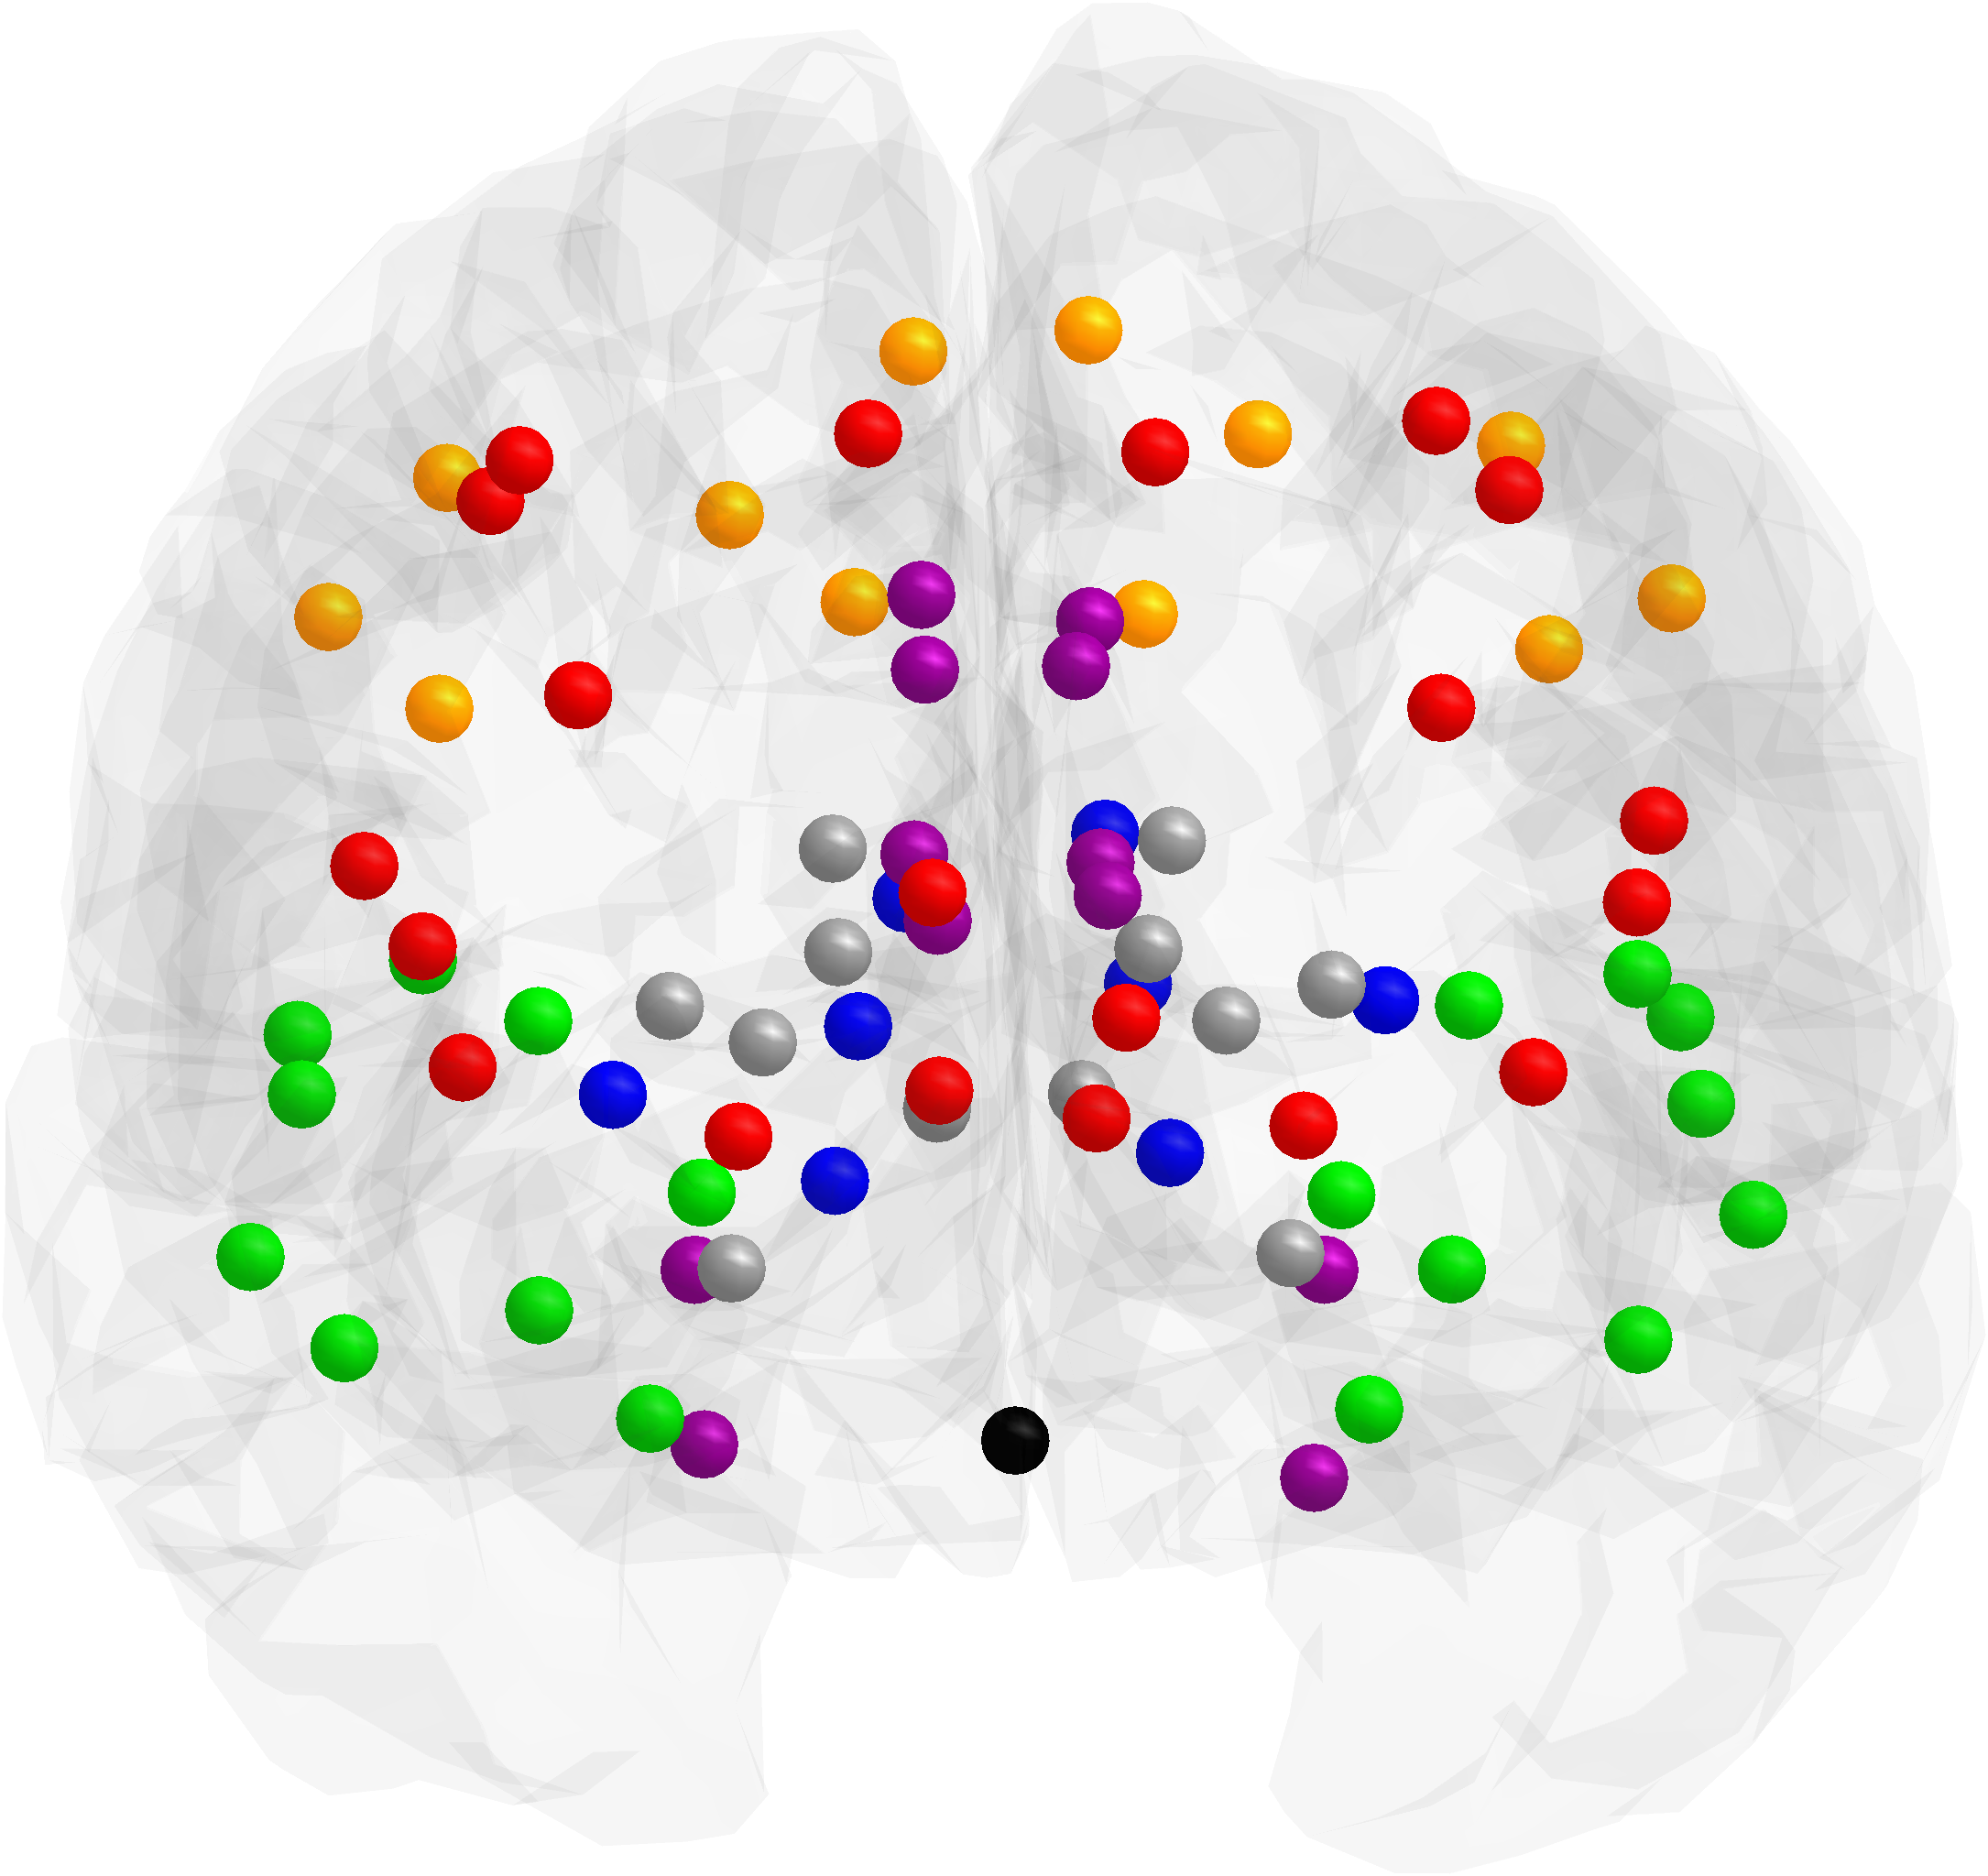
\includegraphics[width=\widthIm cm]
        {../Figure/regioniCervelloFronte [Trasparente].png}};
        % {../Figure/regioniCervelloFronte [Trasparente].png}};
    \node[anchor=north west] at (FKR c1r3.north west)
        {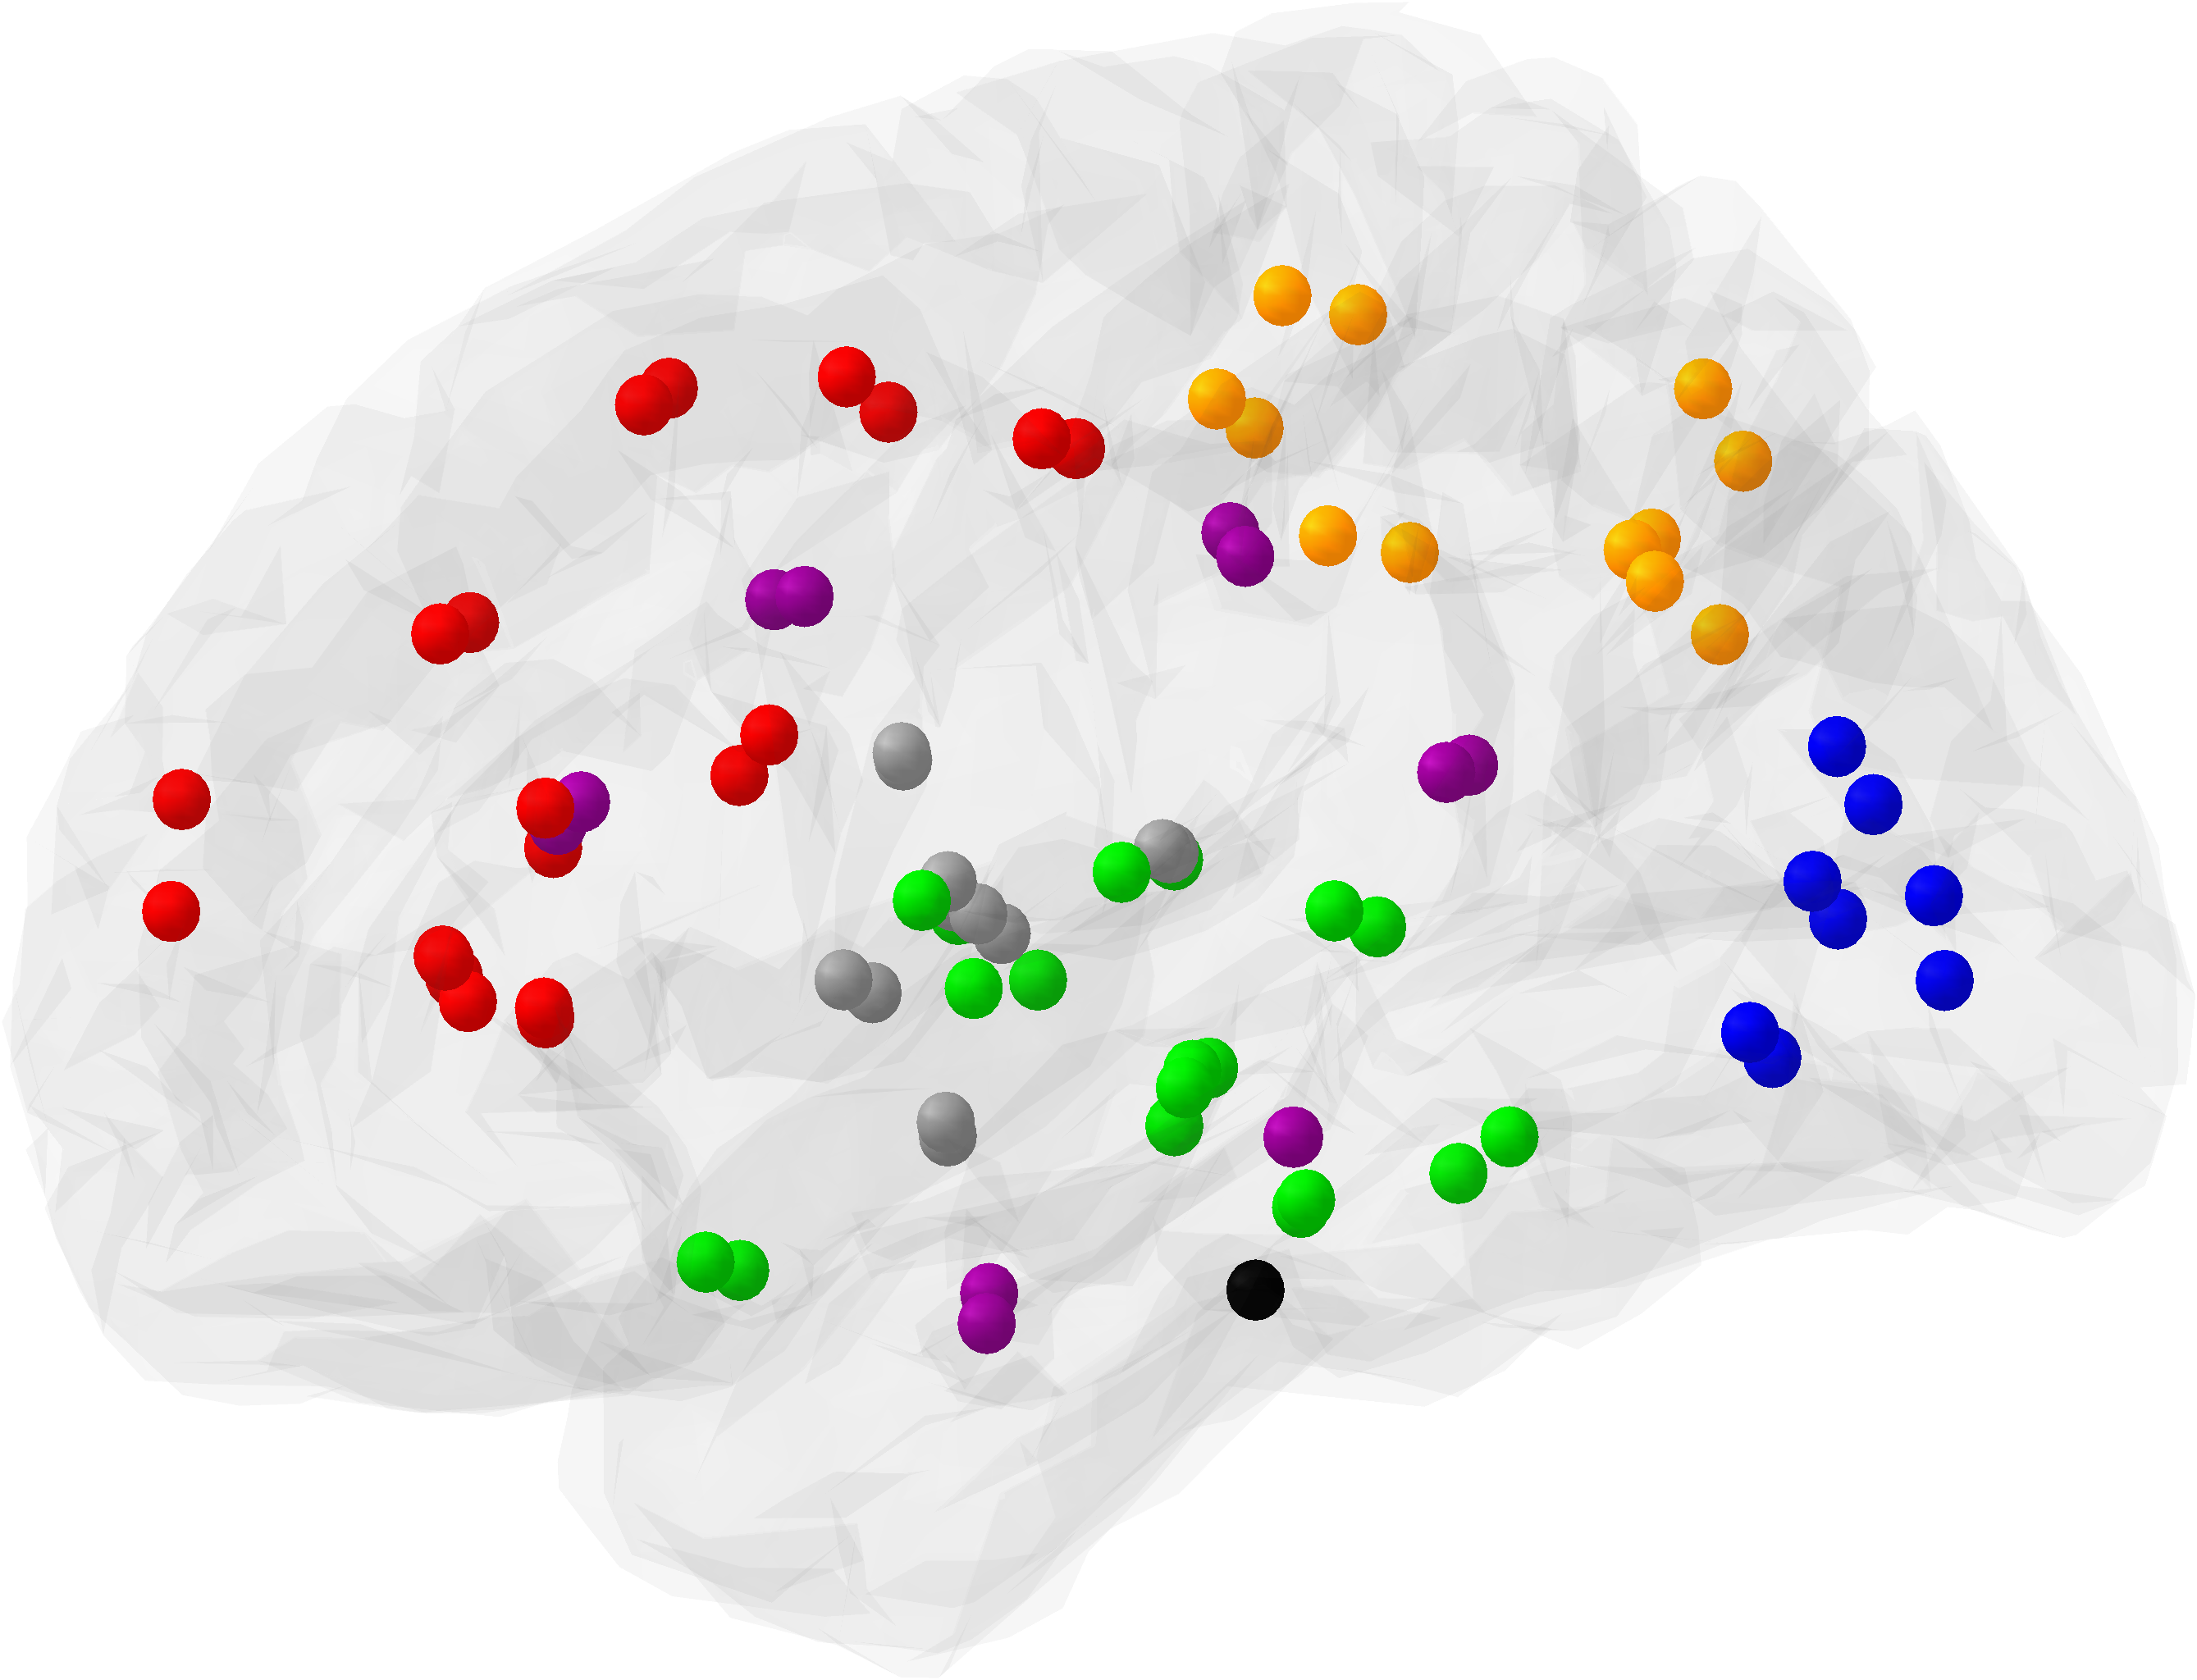
\includegraphics[width=\widthIm cm]
        {../Figure/regioniCervelloLato [Trasparente].png}};
        % {../Figure/regioniCervelloLato [Trasparente].png}};
    \node[anchor=north west] at (FKR c1r4.north west)
        {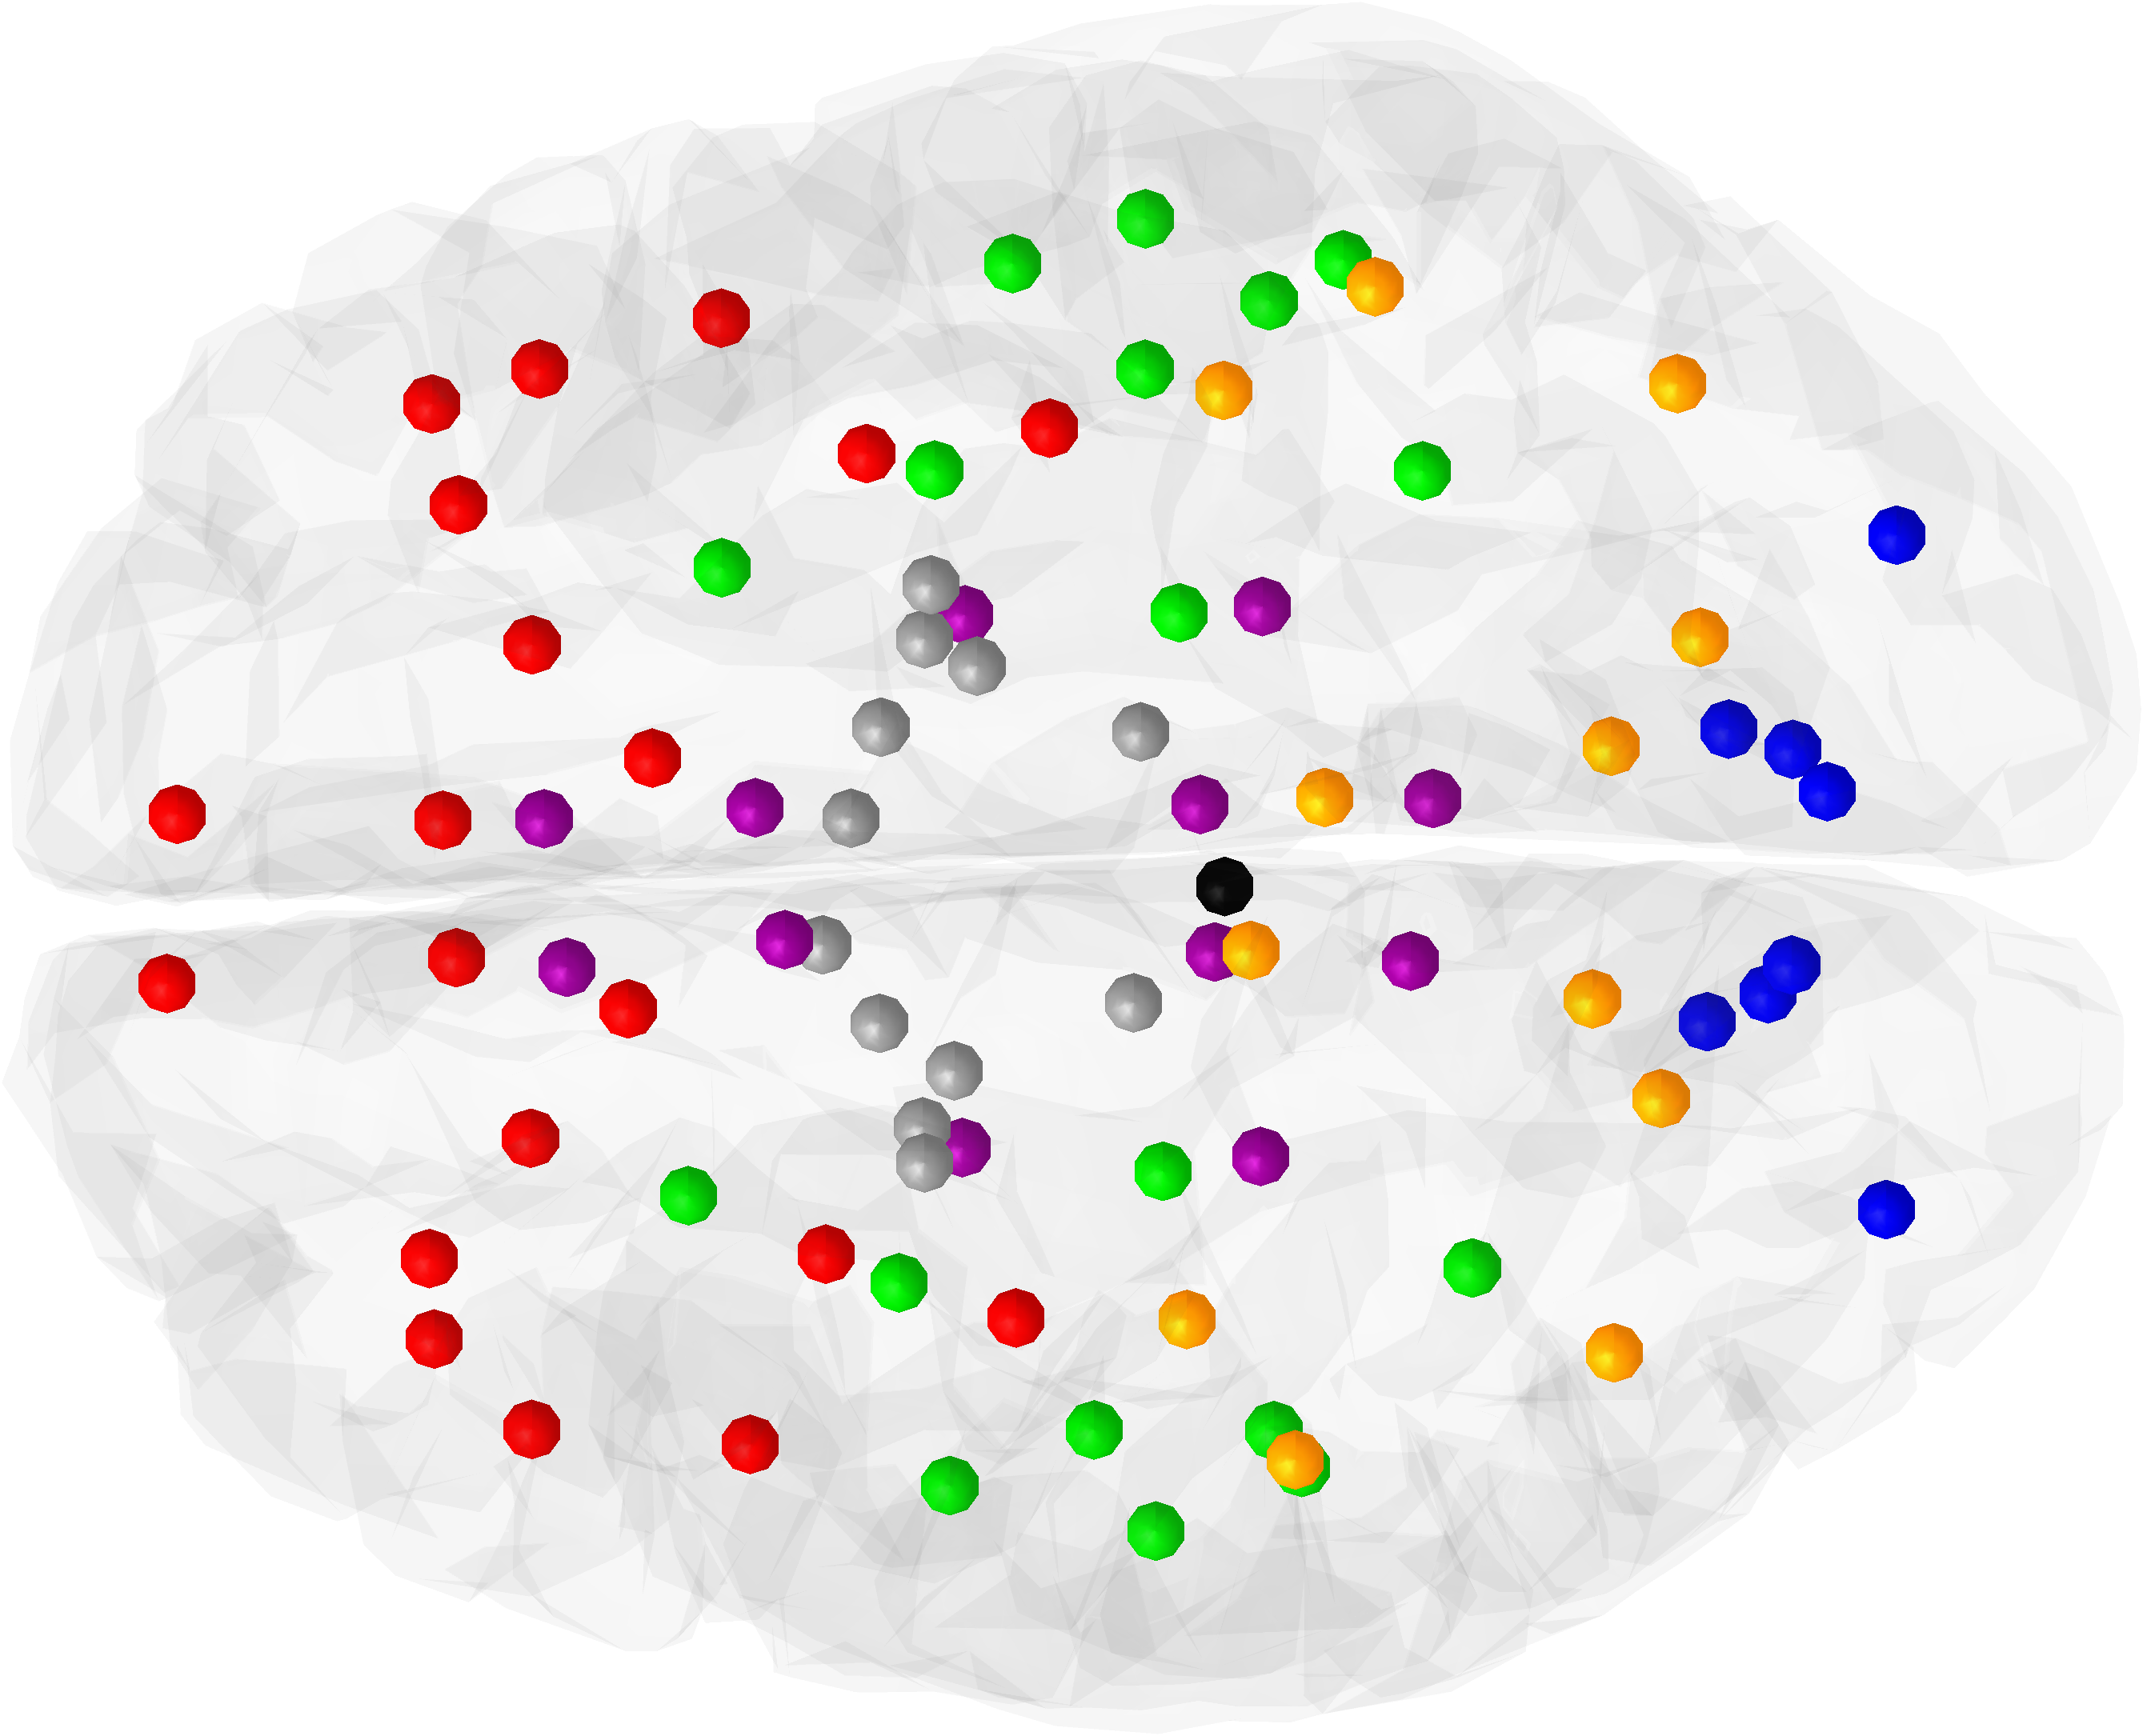
\includegraphics[width=\widthIm cm]
        {../Figure/regioniCervelloAlto [Trasparente].png}};
        % {../Figure/regioniCervelloAlto [Trasparente].png}};

    %
    \tikzset{SubCaption/.style={text width=4cm,anchor=south east,align=right}} %,inner sep=0pt,draw
    \node[SubCaption] at (FKR c1r1.south east)
        {\dimTesto{\captionSize}\sottoDidascalia{\selezionaLingua{$\mathbf L$ statica}{Static $\mathbf L$}\label{figHDStaticL}}};
    \node[SubCaption] at (FKR c1r2.south east)
        {\dimTesto{\captionSize}\sottoDidascalia{\selezionaLingua{$\mathbf L$ dinamica}{Dynamic $\mathbf L$}\label{figHDDynamicL}}};
    \node[SubCaption] at (FKR c1r3.south east)
        {\dimTesto{\captionSize}\sottoDidascalia{$f_d^l\leftrightarrow f_d^h$ variant\label{figHDDynamicLVariant1}}};
    \node[SubCaption] at (FKR c1r4.south east)
        {\dimTesto{\captionSize}\sottoDidascalia{$f_d^l\leftrightarrow f_d^m$ variant\label{figHDDynamicLVariant2}}};

    \node[SubCaption] at (FKN c1r1.south east)
        {\dimTesto{\captionSize}\sottoDidascalia{\selezionaLingua{Rete}{Network}\label{figHDNetwork}}};
    \node[SubCaption] at (FKN c1r2.south east)
        {\dimTesto{\captionSize}\sottoDidascalia{\selezionaLingua{Temporale}{Temporal}\label{figHDTemporal}}};
    \node[SubCaption] at (FKN c1r3.south east)
        {\dimTesto{\captionSize}\sottoDidascalia{\selezionaLingua{Frontale}{Frontal}\label{figHDFrontal}}};
    \node[SubCaption] at (FKN c1r4.south east)
        {\dimTesto{\captionSize}\sottoDidascalia{\selezionaLingua{Parietale}{Parietal}\label{figHDParietal}}};
    \node[SubCaption] at (FKN c1r5.south east)
        {\dimTesto{\captionSize}\sottoDidascalia{\selezionaLingua{Occipitale}{Occipital}\label{figHDOccipital}}};
    \node[SubCaption] at (FKN c1r6.south east)
        {\dimTesto{\captionSize}\sottoDidascalia{\selezionaLingua{Limbico}{Limbic}\label{figHDLimbic}}};
    \node[SubCaption] at (FKN c1r7.south east)
        {\dimTesto{\captionSize}\sottoDidascalia{\selezionaLingua{Ganglia basale}{Basal ganglia}\label{figHDBasalGanglia}}};
    \node[SubCaption] at (FKN c1r8.south east)
        {\dimTesto{\captionSize}\sottoDidascalia{\selezionaLingua{Ceppo enfalico}{Brainstem}\label{figHDBrainstem}}};

    % Un'alternativa a quella di aumentare il contantore delle figure prima di «tikzpicture», usare la funzione «\sottoDidascalia{}» e di decrementare il contatore dopo «tikzpicture» è quella di usare «\subcaptionbox{}»
    % https://tex.stackexchange.com/questions/632045/get-subcaption-for-every-plot-using-groupplot-pgf-tikz-after-2020-update
    % Tuttavia il problema è che a volte LaTeX si lamenta con «nullfont», seppure vi sia testo all'interno della didascalia, e che essa non è rigida: non si possono controllare l'allineamento e la dimensione del nodo perfettamente
    % Un'altra possibilità è di scrivere «\caption» o «\captionof» prima della figure flottante e trattare la didascalia come un titolo della figura
\end{tikzpicture}}
                    {\selezionaLingua
                        {Casi studio di \HDdiscrete{}}
                        {\HDdiscrete{} case studies}.}
                    {\linewidth}
                    {figHDCurves}

                %%%%%%%%%%%%%%%%%%%%%%%%
                %%%%%%%%%%%%%%%%%%%%%%%%
                %%%%%%%%%%%%%%%%%%%%%%%%

                \footnotetext{The authors in \cite[§ 4.2]{Fornari2019} suggests the same conclusion but do not prove it, opting instead to discuss some parametric studies of \FKdiscrete{} and \HDdiscrete{} [unfortunately without normalizing the latter].}

                The static $\mathbf L$ case is shown in Figs. \cref{figFKStaticL,figHDStaticL}; in this the \eqref{eqAntiClockwiseSpreading} spreading manifests, whereas the fact the parietal and occipital lobe have overlapping curves is a clear sign of the degeneracy onset (§ \ref{secCharacteristicTimes}) and, indeed, $\tau_d<\tau_g$.

                Conversely, the dynamic $\mathbf L$ case is illustrated in Figs. \cref{figFKDynamicL,figHDDynamicL} where the parietal and occipital lobes do not have overlapping curves any more. Meanwhile, from Figs. \cref{figFKNetwork,figFKTemporal,figFKFrontal,figFKParietal,figFKOccipital,figFKLimbic,figFKBasalGanglia,figFKBrainstem,figHDNetwork,figHDTemporal,figHDFrontal,figHDParietal,figHDOccipital,figHDLimbic,figHDBasalGanglia,figHDBrainstem} it's clear the presence of a slight global delay, that is to say that at one time the concentration is less than in $\mathbf L$ static case.

                Nevertheless, overall the difference between the sta\-tic and dynamic $\mathbf L$ cases is very minimal considering all \num{5785} low value edges die out in about 1/3 of the dynamic: this implies their influence is small. To test this intuition we have proposed two variants: one where $f_d^l$ is swapped with $f_d^h$ and the other with $f_d^m$, represented with
                %
                \begin{subequations}
                    \begin{align}
                        f_d^l\leftrightarrow f_d^h\tag{V1}\label{eqLDVariantI},\\
                        f_d^l\leftrightarrow f_d^m\tag{V2}\label{eqLDVariantII}.
                    \end{align}
                \end{subequations}
                %
                The goal is to see how the network behaves if the medium and high value edges die out very early in the dynamic.

                The \eqref{eqLDVariantI} case can be seen in Figs. \cref{figFKDynamicLVariant1,figHDDynamicLVariant1} and are very similar to the dynamic $\mathbf L$ case. From Figs. \cref{figFKNetwork,figFKTemporal,figFKFrontal,figFKParietal,figFKOccipital,figFKLimbic,figFKBasalGanglia,figFKBrainstem,figHDNetwork,figHDTemporal,figHDFrontal,figHDParietal,figHDOccipital,figHDLimbic,figHDBasalGanglia,figHDBrainstem} it's evidently a middle way between the static and dynamic $\mathbf L$ cases. Consequently, the few \num{10} high value edges are not really relevant for the diffusion phenomenon.

                On the contrary, the \eqref{eqLDVariantII} case is shown in Figs. \cref{figFKDynamicLVariant2,figHDDynamicLVariant2} and appears to be very different: the basal ganglia outgrow the brainstem concentration, while the Limbic system slows down and is outgrown by the parietal lobe around the end. From Figs. \cref{figFKNetwork,figFKTemporal,figFKFrontal,figFKParietal,figFKOccipital,figFKLimbic,figFKBasalGanglia,figFKBrainstem,figHDNetwork,figHDTemporal,figHDFrontal,figHDParietal,figHDOccipital,figHDLimbic,figHDBasalGanglia,figHDBrainstem}, instead, it's clear this is by far the most delayed dynamic of all, aside from the temporal lobe.

                Therefore, the \eqref{eqLDVariantII} case hints at the importance of the \num{1094} medium value edges for the dynamic of misfolded $\tau$ proteins. One could attribute this behaviour to the bigger increase of the diffusive timescale $\tau_d$, but Fig. \ref{figDynamicDiffusiveTimeScales} proves this may not the case: the \eqref{eqLDVariantII} $\tau_d$ increases more in the first half but is then surpassed in value by the \eqref{eqLDVariantI} $\tau_d$; at any rate, they still remain in the same OOM of $\tau_g$, far from the hiccup evolution described in § \ref{secCharacteristicTimes}.

                \begin{figure}[htb]
                    \centering
                    \resizebox{\linewidth}{!}{% This file was created by matlab2tikz.
%
%The latest updates can be retrieved from
%  http://www.mathworks.com/matlabcentral/fileexchange/22022-matlab2tikz-matlab2tikz
%where you can also make suggestions and rate matlab2tikz.

% This code was later modified by Valerio Taralli

\begin{tikzpicture}%[every node/.style={font=\tSizeLabel}]
    \pgfmathsetmacro\fSizeLabel{10.95}
    \pgfmathsetmacro\baseline{\fSizeLabel*1.2}
    \newcommand\tSizeLabel{\fontsize{\fSizeLabel pt}{\baseline pt}\selectfont}

    \pgfmathsetmacro\fSizeLegend{8}
    \pgfmathsetmacro\baseline{\fSizeLegend*1.2}
    \newcommand\tSizeLegend{\fontsize{\fSizeLegend pt}{\baseline pt}\selectfont}

    \pgfmathsetmacro\lineWidth{.75}
    \pgfmathsetmacro\numMarker{10}
    \pgfmathsetmacro\sizeMarker{1.5}

    \pgfmathsetmacro\yScale{0.75}

    \pgfplotsset{
        markOption/.style={
            mark options={solid,magenta},
            mark repeat=\numMarker,
            mark size=\sizeMarker pt,
            mark phase=\numMarker
        },
        markX/.style={markOption,mark=x},
        markO/.style={markOption,mark=o},
        mark+/.style={markOption,mark=+},
    }

    \begin{axis}[%
                axis lines=middle,
                scale only axis,
                xmin=0,xmax=60,
                xlabel style={font=\color{white!15!black}\tSizeLabel},
                xlabel={$t$ [\unit{\year}]},
                xtick distance=5,
                ymin=1,ymax=10,
                ylabel style={font=\color{white!15!black}\tSizeLabel},
                ylabel={$\tau_D$ [\unit{\year}]},
                ytick distance=1,
                y post scale=\yScale,
                axis background/.style={fill=white},
                axis x line*=bottom,
                axis y line*=left,
                xmajorgrids,
                ymajorgrids,
                grid style={dashed},
                legend style={legend cell align=left,
                            align=left,
                            at={(0,.75)}, % Misure normalizzate
                            anchor=west,
                            xshift=1 cm,
                            draw=white!15!black,
                            font=\tSizeLegend,
                            % fill=none,
                            % draw=none,
                            },
                ]
        \addplot [color=black,line width=\lineWidth pt,markX]
        table[row sep=crcr]{%
        0	1\\
        0.606060606060606	1.04813621355273\\
        1.21212121212121	1.095275238664\\
        1.81818181818182	1.14150405792008\\
        2.42424242424242	1.18690247077015\\
        3.03030303030303	1.23154291697188\\
        3.63636363636364	1.27549067683514\\
        4.24242424242424	1.3188042978915\\
        4.84848484848485	1.36153614165862\\
        5.45454545454545	1.40373297831345\\
        6.06060606060606	1.44543658248232\\
        6.66666666666667	1.48668430159766\\
        7.27272727272727	1.52750958095966\\
        7.87878787878788	1.56794243817587\\
        8.48484848484848	1.60800988517472\\
        9.09090909090909	1.64773629938345\\
        9.6969696969697	1.68714374759315\\
        10.3030303030303	1.72625226698812\\
        10.9090909090909	1.76508010813953\\
        11.5151515151515	1.80364394469639\\
        12.1212121212121	1.84195905421458\\
        12.7272727272727	1.88003947415685\\
        13.3333333333333	1.91789813664443\\
        13.9393939393939	1.95554698508702\\
        14.5454545454545	1.99299707538951\\
        15.1515151515152	2.03025866404242\\
        15.7575757575758	2.06734128505611\\
        16.3636363636364	2.10425381739576\\
        16.969696969697	2.14100454431361\\
        17.5757575757576	2.17760120575271\\
        18.1818181818182	2.21405104480952\\
        18.7878787878788	2.25036084908426\\
        19.3939393939394	2.28653698761708\\
        20	2.32258544399727\\
        20.6060606060606	2.35851184614196\\
        21.2121212121212	2.39432149316417\\
        21.8181818181818	2.43001937968692\\
        22.4242424242424	2.46561021790742\\
        23.030303030303	2.50109845767142\\
        23.6363636363636	2.53648830478107\\
        24.2424242424242	2.57178373772902\\
        24.8484848484848	2.60698852302562\\
        25.4545454545455	2.64210622926443\\
        26.0606060606061	2.6771402400528\\
        26.6666666666667	2.71209376591875\\
        27.2727272727273	2.74696985529209\\
        27.8787878787879	2.7817714046462\\
        28.4848484848485	2.81650116787736\\
        29.0909090909091	2.85116176498975\\
        29.6969696969697	2.88575569014726\\
        30.3030303030303	2.92028531914653\\
        30.9090909090909	2.9547529163603\\
        31.5151515151515	2.98916064119514\\
        32.1212121212121	3.02351055410346\\
        32.7272727272727	3.05780462218547\\
        33.3333333333333	3.09204472441415\\
        33.9393939393939	3.1262326565123\\
        34.5454545454545	3.16037013550905\\
        35.1515151515151	3.19445880399993\\
        35.7575757575758	3.22850023413311\\
        36.3636363636364	3.26249593134214\\
        36.969696969697	3.2964473378438\\
        37.5757575757576	3.3303558359183\\
        38.1818181818182	3.36422275098735\\
        38.7878787878788	3.39804935450465\\
        39.3939393939394	3.43183686667188\\
        40	3.46558645899246\\
        40.6060606060606	3.49929925667426\\
        41.2121212121212	3.53297634089152\\
        41.8181818181818	3.56661875091561\\
        42.4242424242424	3.60022748612334\\
        43.030303030303	3.63380350789097\\
        43.6363636363636	3.66734774138145\\
        44.2424242424242	3.7008610772318\\
        44.8484848484849	3.73434437314716\\
        45.4545454545455	3.76779845540736\\
        46.0606060606061	3.80122412029164\\
        46.6666666666667	3.83462213542661\\
        47.2727272727273	3.86799324106229\\
        47.8787878787879	3.90133815128056\\
        48.4848484848485	3.9346575551403\\
        49.0909090909091	3.96795211776286\\
        49.6969696969697	4.00122248136168\\
        50.3030303030303	4.03446926621916\\
        50.9090909090909	4.06769307161411\\
        51.5151515151515	4.10089447670248\\
        52.1212121212121	4.13407404135423\\
        52.7272727272727	4.16723230694879\\
        53.3333333333333	4.20036979713152\\
        53.9393939393939	4.23348701853335\\
        54.5454545454545	4.2665844614557\\
        55.1515151515151	4.29966260052259\\
        55.7575757575758	4.33272189530177\\
        56.3636363636364	4.36576279089659\\
        56.969696969697	4.39878571851016\\
        57.5757575757576	4.43179109598338\\
        58.1818181818182	4.4647793283081\\
        58.7878787878788	4.49775080811693\\
        59.3939393939394	4.53070591615075\\
        60	4.56364502170521\\
        };
        \addlegendentry{Dynamic L}

        \addplot [color=red,line width=\lineWidth pt,markO]
        table[row sep=crcr]{%
		0	1\\
		0.606060606060606	1.13090547003089\\
		1.21212121212121	1.26026296827647\\
		1.81818181818182	1.38594918487567\\
		2.42424242424242	1.50660352040334\\
		3.03030303030303	1.62162389867056\\
		3.63636363636364	1.73103675406443\\
		4.24242424242424	1.83529377644278\\
		4.84848484848485	1.93506210254601\\
		5.45454545454545	2.03105875301759\\
		6.06060606060606	2.12394558346075\\
		6.66666666666667	2.21427103968054\\
		7.27272727272727	2.3024288875846\\
		7.87878787878788	2.38861128947633\\
		8.48484848484848	2.47288197109407\\
		9.09090909090909	2.5556083898498\\
		9.6969696969697	2.63744285445858\\
		10.3030303030303	2.71881906110576\\
		10.9090909090909	2.79993600232202\\
		11.5151515151515	2.88088646619214\\
		12.1212121212121	2.96171954205808\\
		12.7272727272727	3.04246451695215\\
		13.3333333333333	3.12314052119\\
		13.9393939393939	3.20376087236852\\
		14.5454545454545	3.2843352583854\\
		15.1515151515152	3.36487094614224\\
		15.7575757575758	3.44537350763658\\
		16.3636363636364	3.52584728603434\\
		16.969696969697	3.60629571092102\\
		17.5757575757576	3.68672152031634\\
		18.1818181818182	3.76712692186161\\
		18.7878787878788	3.8475137125192\\
		19.3939393939394	3.92788336894547\\
		20	4.00823711654354\\
		20.6060606060606	4.08857598268079\\
		21.2121212121212	4.16890083795421\\
		21.8181818181818	4.24921242832741\\
		22.4242424242424	4.32951140023729\\
		23.030303030303	4.40979832025353\\
		23.6363636363636	4.49007369050084\\
		24.2424242424242	4.57033796077615\\
		24.8484848484848	4.65059153808358\\
		25.4545454545455	4.73083479414988\\
		26.0606060606061	4.81106807135951\\
		26.6666666666667	4.89129168745276\\
		27.2727272727273	4.97150593925543\\
		27.8787878787879	5.05171110565013\\
		28.4848484848485	5.13190744995379\\
		29.0909090909091	5.21209522182972\\
		29.6969696969697	5.29227465883488\\
		30.3030303030303	5.37244598768069\\
		30.9090909090909	5.45260942526884\\
		31.5151515151515	5.53276517954971\\
		32.1212121212121	5.61291345024097\\
		32.7272727272727	5.69305442943526\\
		33.3333333333333	5.77318830211969\\
		33.9393939393939	5.85331524662499\\
		34.5454545454545	5.93343543501799\\
		35.1515151515151	6.01354903344841\\
		35.7575757575758	6.09365620245823\\
		36.3636363636364	6.17375709726044\\
		36.969696969697	6.25385186799235\\
		37.5757575757576	6.33394065994751\\
		38.1818181818182	6.41402361378959\\
		38.7878787878788	6.49410086575073\\
		39.3939393939394	6.57417254781657\\
		40	6.65423878789947\\
		40.6060606060606	6.73429971000137\\
		41.2121212121212	6.81435543436739\\
		41.8181818181818	6.89440607763109\\
		42.4242424242424	6.97445175295219\\
		43.030303030303	7.05449257014723\\
		43.6363636363636	7.13452863581398\\
		44.2424242424242	7.21456005344989\\
		44.8484848484849	7.29458692356499\\
		45.4545454545455	7.37460934378973\\
		46.0606060606061	7.45462740897794\\
		46.6666666666667	7.53464121130536\\
		47.2727272727273	7.61465084036376\\
		47.8787878787879	7.69465638325117\\
		48.4848484848485	7.7746579246582\\
		49.0909090909091	7.85465554695085\\
		49.6969696969697	7.93464933024976\\
		50.3030303030303	8.01463935250637\\
		50.9090909090909	8.09462568957581\\
		51.5151515151515	8.17460841528702\\
		52.1212121212121	8.25458760150995\\
		52.7272727272727	8.3345633182201\\
		53.3333333333333	8.41453563356061\\
		53.9393939393939	8.49450461390184\\
		54.5454545454545	8.57447032389861\\
		55.1515151515151	8.65443282654535\\
		55.7575757575758	8.73439218322899\\
		56.3636363636364	8.81434845377996\\
		56.969696969697	8.8943016965212\\
		57.5757575757576	8.97425196831533\\
		58.1818181818182	9.05419932461009\\
		58.7878787878788	9.13414381948203\\
		59.3939393939394	9.21408550567869\\
		60	9.29402443465915\\
        };
        \addlegendentry{\selezionaLingua{Variante}{Variant} $f_d^l\leftrightarrow f_d^h$}

        \addplot [color=blue,line width=\lineWidth pt,mark+]
        table[row sep=crcr]{%
		0	1\\
		0.606060606060606	1.23157394286427\\
		1.21212121212121	1.48555432016994\\
		1.81818181818182	1.7530935631925\\
		2.42424242424242	2.02364341513464\\
		3.03030303030303	2.1898147667142\\
		3.63636363636364	2.28863911450774\\
		4.24242424242424	2.37447754371903\\
		4.84848484848485	2.44957005115134\\
		5.45454545454545	2.51594677771319\\
		6.06060606060606	2.57536455902643\\
		6.66666666666667	2.62929222133281\\
		7.27272727272727	2.67892768556717\\
		7.87878787878788	2.72523041296043\\
		8.48484848484848	2.76895869673147\\
		9.09090909090909	2.81070593605534\\
		9.6969696969697	2.85093307005815\\
		10.3030303030303	2.88999616295111\\
		10.9090909090909	2.92816911791309\\
		11.5151515151515	2.96566197242\\
		12.1212121212121	3.00263540803651\\
		12.7272727272727	3.03921213042214\\
		13.3333333333333	3.07548572219495\\
		13.9393939393939	3.1115274883704\\
		14.5454545454545	3.147391725656\\
		15.1515151515152	3.18311976462894\\
		15.7575757575758	3.21874306246103\\
		16.3636363636364	3.25428556443444\\
		16.969696969697	3.28976550430087\\
		17.5757575757576	3.32519677514382\\
		18.1818181818182	3.3605899721953\\
		18.7878787878788	3.39595318550073\\
		19.3939393939394	3.43129260207488\\
		20	3.46661296312014\\
		20.6060606060606	3.50191791106882\\
		21.2121212121212	3.53721025293063\\
		21.8181818181818	3.57249216009718\\
		22.4242424242424	3.60776531992505\\
		23.030303030303	3.64303105073849\\
		23.6363636363636	3.67829038909092\\
		24.2424242424242	3.71354415599347\\
		24.8484848484848	3.74879300719924\\
		25.4545454545455	3.78403747140241\\
		26.0606060606061	3.81927797927729\\
		26.6666666666667	3.85451488557435\\
		27.2727272727273	3.88974848595301\\
		27.8787878787879	3.92497902982366\\
		28.4848484848485	3.9602067301629\\
		29.0909090909091	3.99543177103188\\
		29.6969696969697	4.03065431335084\\
		30.3030303030303	4.06587449934841\\
		30.9090909090909	4.10109245600315\\
		31.5151515151515	4.13630829771746\\
		32.1212121212121	4.1715221284061\\
		32.7272727272727	4.2067340431374\\
		33.3333333333333	4.24194412943195\\
		33.9393939393939	4.27715246829815\\
		34.5454545454545	4.31235913506519\\
		35.1515151515151	4.34756420005932\\
		35.7575757575758	4.3827677291584\\
		36.3636363636364	4.41796978425145\\
		36.969696969697	4.45317042362353\\
		37.5757575757576	4.48836970228175\\
		38.1818181818182	4.52356767223412\\
		38.7878787878788	4.5587643827308\\
		39.3939393939394	4.59395988047473\\
		40	4.62915420980721\\
		40.6060606060606	4.66434741287289\\
		41.2121212121212	4.69953952976744\\
		41.8181818181818	4.73473059867074\\
		42.4242424242424	4.76992065596757\\
		43.030303030303	4.8051097363578\\
		43.6363636363636	4.84029787295715\\
		44.2424242424242	4.87548509738995\\
		44.8484848484849	4.9106714398747\\
		45.4545454545455	4.94585692930322\\
		46.0606060606061	4.98104159331413\\
		46.6666666666667	5.01622545836115\\
		47.2727272727273	5.05140854977678\\
		47.8787878787879	5.08659089183166\\
		48.4848484848485	5.12177250779017\\
		49.0909090909091	5.15695341996231\\
		49.6969696969697	5.19213364975249\\
		50.3030303030303	5.22731321770518\\
		50.9090909090909	5.26249214354782\\
		51.5151515151515	5.29767044623118\\
		52.1212121212121	5.33284814396725\\
		52.7272727272727	5.36802525426502\\
		53.3333333333333	5.40320179396405\\
		53.9393939393939	5.43837777926626\\
		54.5454545454545	5.47355322576584\\
		55.1515151515151	5.50872814847748\\
		55.7575757575758	5.54390256186307\\
		56.3636363636364	5.57907647985694\\
		56.969696969697	5.61424991588968\\
		57.5757575757576	5.6494228829107\\
		58.1818181818182	5.68459539340964\\
		58.7878787878788	5.71976745943654\\
		59.3939393939394	5.75493909262107\\
		60	5.79011030419065\\
        };
        \addlegendentry{\selezionaLingua{Variante}{Variant} $f_d^l\leftrightarrow f_d^m$}
    \end{axis}
\end{tikzpicture}}
                    % \captionsetup{width=0.5\linewidth}
                    \caption{Dynamic diffusive timescale.}
                    \label{figDynamicDiffusiveTimeScales}
                \end{figure}

                Lastly, it's noteworthy that the convergence time increases only slightly in all cases, confirming \ref{rmkDiffusionContributionConvergenceTime}.

            \subsubsection{SMO model}\label{secResultsSMO}

                %%%%%%%%%%%%%%%%%%%%%%
                %%% Infopagina SMO %%%
                %%%%%%%%%%%%%%%%%%%%%%

                \includetikzgroupplotfigure*{tbp}{-1.6cm}{\textwidth}
                    {% This file was created by matlab2tikz.
%
%The latest updates can be retrieved from
%  http://www.mathworks.com/matlabcentral/fileexchange/22022-matlab2tikz-matlab2tikz
%where you can also make suggestions and rate matlab2tikz.

% This code was later modified by Valerio Taralli

\definecolor{mycolor1M}{rgb}{0.00000,0.00000,0.51562}%
\definecolor{mycolor2M}{rgb}{0.00000,0.00000,0.59375}%
\definecolor{mycolor3M}{rgb}{0.00000,0.00000,0.68750}%
\definecolor{mycolor4M}{rgb}{0.00000,0.01562,1.00000}%
\definecolor{mycolor5M}{rgb}{0.00000,0.09375,1.00000}%
\definecolor{mycolor6M}{rgb}{0.00000,0.18750,1.00000}%
\definecolor{mycolor7M}{rgb}{0.00000,0.26562,1.00000}%
\definecolor{mycolor8M}{rgb}{0.00000,0.34375,1.00000}%
\definecolor{mycolor9M}{rgb}{0.00000,0.42188,1.00000}%
\definecolor{mycolor10M}{rgb}{0.00000,0.51562,1.00000}%
\definecolor{mycolor11M}{rgb}{0.00000,0.59375,1.00000}%
\definecolor{mycolor12M}{rgb}{0.00000,0.67188,1.00000}%
\definecolor{mycolor13M}{rgb}{0.00000,0.76562,1.00000}%
\definecolor{mycolor14M}{rgb}{0.00000,0.84375,1.00000}%
\definecolor{mycolor15M}{rgb}{0.00000,0.92188,1.00000}%
\definecolor{mycolor16M}{rgb}{0.01562,1.00000,0.98438}%
\definecolor{mycolor17M}{rgb}{0.09375,1.00000,0.90625}%
\definecolor{mycolor18M}{rgb}{0.17188,1.00000,0.82812}%
\definecolor{mycolor19M}{rgb}{0.26562,1.00000,0.73438}%
\definecolor{mycolor20M}{rgb}{0.34375,1.00000,0.65625}%
\definecolor{mycolor21M}{rgb}{0.42188,1.00000,0.57812}%
\definecolor{mycolor22M}{rgb}{0.51562,1.00000,0.48438}%
\definecolor{mycolor23M}{rgb}{0.59375,1.00000,0.40625}%
\definecolor{mycolor24M}{rgb}{0.67188,1.00000,0.32812}%
\definecolor{mycolor25M}{rgb}{0.75000,1.00000,0.25000}%
\definecolor{mycolor26M}{rgb}{0.84375,1.00000,0.15625}%
\definecolor{mycolor27M}{rgb}{0.92188,1.00000,0.07812}%
\definecolor{mycolor28M}{rgb}{1.00000,1.00000,0.00000}%
\definecolor{mycolor29M}{rgb}{1.00000,0.90625,0.00000}%
\definecolor{mycolor30M}{rgb}{1.00000,0.82812,0.00000}%
\definecolor{mycolor31M}{rgb}{1.00000,0.65625,0.00000}%
\definecolor{mycolor32M}{rgb}{1.00000,0.40625,0.00000}%
\definecolor{mycolor33M}{rgb}{1.00000,0.15625,0.00000}%
\definecolor{mycolor34M}{rgb}{0.92188,0.00000,0.00000}%
\definecolor{mycolor35M}{rgb}{0.82812,0.00000,0.00000}%
\definecolor{mycolor36M}{rgb}{0.67188,0.00000,0.00000}%
\definecolor{mycolor37M}{rgb}{0.57812,0.00000,0.00000}%
%
%
%
\definecolor{mycolor1D}{rgb}{0.00000,0.00000,0.65625}%
\definecolor{mycolor2D}{rgb}{0.00000,0.00000,0.64062}%
\definecolor{mycolor3D}{rgb}{0.00000,0.00000,0.78125}%
\definecolor{mycolor4D}{rgb}{0.00000,0.00000,0.92188}%
\definecolor{mycolor5D}{rgb}{0.00000,0.00000,0.90625}%
\definecolor{mycolor6D}{rgb}{0.00000,0.04688,1.00000}%
\definecolor{mycolor7D}{rgb}{0.00000,0.18750,1.00000}%
\definecolor{mycolor8D}{rgb}{0.00000,0.17188,1.00000}%
\definecolor{mycolor9D}{rgb}{0.00000,0.31250,1.00000}%
\definecolor{mycolor10D}{rgb}{0.00000,0.45312,1.00000}%
\definecolor{mycolor11D}{rgb}{0.00000,0.43750,1.00000}%
\definecolor{mycolor12D}{rgb}{0.00000,0.57812,1.00000}%
\definecolor{mycolor13D}{rgb}{0.00000,0.71875,1.00000}%
\definecolor{mycolor14D}{rgb}{0.00000,0.70312,1.00000}%
\definecolor{mycolor15D}{rgb}{0.00000,0.84375,1.00000}%
\definecolor{mycolor16D}{rgb}{0.00000,0.98438,1.00000}%
\definecolor{mycolor17D}{rgb}{0.00000,0.96875,1.00000}%
\definecolor{mycolor18D}{rgb}{0.10938,1.00000,0.89062}%
\definecolor{mycolor19D}{rgb}{0.25000,1.00000,0.75000}%
\definecolor{mycolor20D}{rgb}{0.23438,1.00000,0.76562}%
\definecolor{mycolor21D}{rgb}{0.37500,1.00000,0.62500}%
\definecolor{mycolor22D}{rgb}{0.51562,1.00000,0.48438}%
\definecolor{mycolor23D}{rgb}{0.64062,1.00000,0.35938}%
\definecolor{mycolor24D}{rgb}{0.78125,1.00000,0.21875}%
\definecolor{mycolor25D}{rgb}{0.76562,1.00000,0.23438}%
\definecolor{mycolor26D}{rgb}{0.90625,1.00000,0.09375}%
\definecolor{mycolor27D}{rgb}{1.00000,0.95312,0.00000}%
\definecolor{mycolor28D}{rgb}{1.00000,0.96875,0.00000}%
\definecolor{mycolor29D}{rgb}{1.00000,0.70312,0.00000}%
\definecolor{mycolor30D}{rgb}{1.00000,0.43750,0.00000}%
\definecolor{mycolor31D}{rgb}{1.00000,0.29688,0.00000}%
\definecolor{mycolor32D}{rgb}{1.00000,0.15625,0.00000}%
\definecolor{mycolor33D}{rgb}{1.00000,0.17188,0.00000}%
\definecolor{mycolor34D}{rgb}{0.89062,0.00000,0.00000}%
\definecolor{mycolor35D}{rgb}{0.90625,0.00000,0.00000}%
\definecolor{mycolor36D}{rgb}{0.76562,0.00000,0.00000}%
\definecolor{mycolor37D}{rgb}{0.62500,0.00000,0.00000}%
\definecolor{mycolor38D}{rgb}{0.64062,0.00000,0.00000}%

%

\definecolor{mycolor1}{rgb}{1.00000,0.54510,0.00000}%
\definecolor{mycolor2}{rgb}{0.50588,0.00000,0.49804}%
\definecolor{mycolor3}{rgb}{0.00000,0.74510,0.00000}%
\definecolor{mycolor4}{rgb}{0.50196,0.50196,0.50196}%

%

\controllaClasse{% Classe «article»
    \begin{tikzpicture}
        \newcommand\titleSize{12} % Dimensione del titolo
        \newcommand\captionSize{12} % Dimensione dell'etichette
        \newcommand\labelSize{12} % Dimensione dell'etichette
        \newcommand\tickSize{12} % Dimensioni delle tacche
        \newcommand\legendSize{9} % Dimensione della legenda

        \pgfmathsetmacro\widthPlot{10}
        \pgfmathsetmacro\heightPlot{.6*\widthPlot}
        \pgfmathsetmacro\lineWidth{.5pt}
        \pgfmathsetmacro\lineMidWidth{.75pt}
        \pgfmathsetmacro\lineThickWidth{1.2pt}
        
        \pgfmathsetmacro\xPlotSep{.5cm}
        \pgfmathsetmacro\yPlotSep{.5cm}
        \pgfmathsetmacro\xLegendSep{.25cm}

        \pgfplotsset{
            /pgfplots/group/plotGroup/.style={
                group name=SMOM,
                group size=1 by 4,
                vertical sep=\yPlotSep,
                x descriptions at=edge bottom,
                y descriptions at=edge left,
            },
            plotColumn/.style={
                width=\widthPlot cm,% 10.45in
                height=\heightPlot cm,% height=6.328in,
                scale only axis, % Fondamentale per avere coerenza tra i due grafici,altrimenti non scalano correttamente
                xmin=0,xmax=60,
                xlabel={$t$ [\unit{\year}]},
                xlabel style={
                    font=\color{white!15!black}\dimTesto{\labelSize},
                    % at={(ticklabel cs:1.0)},
                    % anchor=east,
                    % yshift=-.3cm,
                },
                xtick distance=5,
                ymin=0,
                ylabel={$c$ [\%]},
                ylabel style={
                    font=\color{white!15!black}\dimTesto{\labelSize},
                    % at={(ticklabel cs:1.0)},
                    % anchor=east,
                    % yshift=.3cm,
                },
                xticklabel style={font=\dimTesto{\tickSize}},
                yticklabel style={font=\dimTesto{\tickSize}},
                % axis background/.style={fill=white},
                axis x line*=bottom,
                axis y line*=left,
                xmajorgrids,
                ymajorgrids,
                grid style={dashed},
            },
            plotLegend/.style={
                legend cell align=left,
                align=left,
                % legend pos=north west,
                at={(0,.5)},
                anchor=west,
                xshift=\xLegendSep,
                draw=white!15!black,
                font=\dimTesto{\legendSize},
                % fill=none,
                % draw=none,
            },
        }

        \begin{groupplot}[group style=plotGroup,plotColumn]
            \nextgroupplot[
                            title style={font=\dimTesto{\titleSize}},
                            title={\selezionaLingua{Massa aggregata}{Aggregate mass}},
                            legend style=plotLegend,
                            ymax=1,
                            ytick distance=.1,
                        ]
            %\begingroup SMO Massa Statico
            \addplot [color=mycolor1M,line width=\lineThickWidth]
            table[row sep=crcr]{%
            0	0\\
            5.4	0.000195412568196218\\
            9.8	0.000863996329840688\\
            16.24	0.00219171976370802\\
            17.68	0.00298292717803861\\
            18.92	0.00405481936029162\\
            20	0.0053709496526082\\
            21	0.00697079258258526\\
            21.96	0.00889834839751558\\
            22.88	0.0111339671253887\\
            23.8	0.0137547531237558\\
            24.8	0.0170048069470425\\
            26.08	0.0215996544575745\\
            27.8	0.0277533846182294\\
            28.56	0.0300557409875353\\
            29.2	0.0316019542162991\\
            29.76	0.0325709659017974\\
            30.28	0.0330949460750674\\
            30.8	0.033222516619027\\
            31.32	0.0329380965628729\\
            31.84	0.0322465637173082\\
            32.4	0.0310768007101245\\
            33	0.029399132977062\\
            33.68	0.0270875468818375\\
            34.64	0.0233887817038507\\
            36.32	0.0168831104201814\\
            37.2	0.0139157315916023\\
            38	0.011607843118064\\
            38.8	0.00968459290169221\\
            39.64	0.00805181594939341\\
            40.56	0.00665501901541887\\
            41.64	0.00542711359202741\\
            42.96	0.00435171496423692\\
            44.64	0.00340059695946593\\
            46.8	0.00258271476172212\\
            49.4	0.00200603153957246\\
            52.84	0.00167346932531132\\
            59.2	0.00153154846157122\\
            60	0.00152708306978155\\
            };
            \addlegendentry{M$_{50}$}
            
            \addplot [color=mycolor2M,line width=\lineWidth,forget plot]
            table[row sep=crcr]{%
            0	0\\
            5.32	0.000197207978544611\\
            9.56	0.000856027175636598\\
            16.2	0.0022603046766605\\
            17.64	0.00307245560306058\\
            18.84	0.00413172658200267\\
            19.92	0.00547100278753021\\
            20.92	0.00710244946301231\\
            21.88	0.00907200623984039\\
            22.8	0.0113610050753934\\
            23.72	0.014050421133355\\
            24.68	0.0172536891649244\\
            25.88	0.0216849913757358\\
            27.8	0.0288294083747473\\
            28.56	0.0312103839144982\\
            29.16	0.0327183060032397\\
            29.72	0.0337413022962281\\
            30.24	0.0343025306161735\\
            30.76	0.0344526664269296\\
            31.24	0.0342111682360979\\
            31.76	0.0335408375081983\\
            32.28	0.0324697808075385\\
            32.84	0.0309204815100657\\
            33.48	0.0287464309863168\\
            34.32	0.0254661652875683\\
            36.52	0.0166781422725109\\
            37.36	0.0138430902094839\\
            38.16	0.0115478446340944\\
            38.96	0.00964931154000936\\
            39.8	0.00804672931052153\\
            40.76	0.00662940384658839\\
            41.84	0.00544320698512024\\
            43.16	0.00439888750891981\\
            44.88	0.00344749246567488\\
            47.08	0.00263677725322964\\
            49.68	0.00208527269507641\\
            53.2	0.00176879938135954\\
            59.96	0.00163800169124073\\
            60	0.00163780148286463\\
            };
            \addplot [color=mycolor3M,line width=\lineWidth,forget plot]
            table[row sep=crcr]{%
            0	0\\
            5.2	0.000195461551328435\\
            9.28	0.000842238491216563\\
            16.16	0.00234093844002814\\
            17.56	0.00314769415462735\\
            18.76	0.00422625236272012\\
            19.84	0.00559359778161905\\
            20.84	0.0072630021982647\\
            21.76	0.00918980266937552\\
            22.64	0.0114137444799809\\
            23.52	0.0140207107268751\\
            24.44	0.0171361495010913\\
            25.52	0.0212070066900196\\
            28.04	0.0309069916566642\\
            28.72	0.0330097245070675\\
            29.32	0.0344651195116725\\
            29.84	0.0353479494741364\\
            30.36	0.0358275224663345\\
            30.84	0.0358835552299652\\
            31.32	0.035557172709396\\
            31.8	0.034854280496269\\
            32.32	0.0336947465712285\\
            32.88	0.0320392781309309\\
            33.52	0.0297373271367931\\
            34.36	0.0262916905203596\\
            36.4	0.0177697600884201\\
            37.2	0.0149023700705442\\
            37.96	0.0125569288028728\\
            38.76	0.0104955661071529\\
            39.6	0.00874949367342026\\
            40.52	0.00725901851405553\\
            41.56	0.00599272442949683\\
            42.8	0.00489531947962263\\
            44.4	0.00389528387455584\\
            46.48	0.00301068288212036\\
            48.92	0.00237851222613017\\
            52.04	0.00199536372554121\\
            57.24	0.00181326426292827\\
            60	0.0017899798763068\\
            };
            \addplot [color=blue!25!mycolor3M,line width=\lineWidth,forget plot]
            table[row sep=crcr]{%
            0	0\\
            5.08	0.000194447439419321\\
            9.04	0.000837426558291554\\
            16.08	0.00241732433635633\\
            17.48	0.00323850862866948\\
            18.64	0.00429626037904285\\
            19.68	0.00562184016248324\\
            20.64	0.00722590649148458\\
            21.56	0.00915554239180238\\
            22.44	0.0113949017374821\\
            23.32	0.0140353649181151\\
            24.2	0.0170663866808027\\
            25.2	0.0209191084690872\\
            26.96	0.0282135418189213\\
            27.92	0.0319568409044919\\
            28.6	0.0342339749434402\\
            29.2	0.035845225165076\\
            29.72	0.0368587604539172\\
            30.2	0.0374286120570986\\
            30.68	0.0376151335532171\\
            31.16	0.037401853031831\\
            31.64	0.0367892605174376\\
            32.12	0.0357957221423391\\
            32.64	0.0343310368984149\\
            33.24	0.0322224343339244\\
            33.96	0.029266398548863\\
            35.44	0.0226471422878731\\
            36.4	0.0185901219831379\\
            37.2	0.0156012113318695\\
            37.96	0.0131606374863509\\
            38.72	0.0111161936936099\\
            39.52	0.00936281706709252\\
            40.4	0.0078427558045604\\
            41.4	0.00653063322447878\\
            42.6	0.00537748069074695\\
            44.12	0.00433863490930264\\
            46.08	0.00341182636666559\\
            48.4	0.00271609486429725\\
            51.24	0.00227952931497555\\
            55.6	0.00205146675491363\\
            60	0.00199798894007586\\
            };
            \addplot [color=blue!50!mycolor3M,line width=\lineWidth,forget plot]
            table[row sep=crcr]{%
            0	0\\
            4.96	0.000194106246034664\\
            8.76	0.000825791537195641\\
            16	0.00250786834936179\\
            17.4	0.00334610526068957\\
            18.56	0.00442955353945251\\
            19.6	0.00579133735715942\\
            20.56	0.00744330050353881\\
            21.44	0.00933960052474703\\
            22.32	0.0116375972296368\\
            23.16	0.0142242863746773\\
            24.04	0.0173408707760316\\
            25	0.0211632000694948\\
            26.28	0.0267086664530396\\
            27.68	0.0326958307831546\\
            28.4	0.0353768523833722\\
            29	0.0372229706459493\\
            29.52	0.0384471716730275\\
            30	0.0392101812211862\\
            30.48	0.0395810931395033\\
            30.96	0.0395355742398706\\
            31.44	0.0390663751359526\\
            31.92	0.0381849867661899\\
            32.4	0.0369216158314387\\
            32.96	0.0350284936894525\\
            33.6	0.0324327251236838\\
            34.48	0.0284072267130355\\
            36.2	0.020459142801819\\
            37	0.0172206377546473\\
            37.76	0.0145558121091938\\
            38.48	0.0124187813810792\\
            39.24	0.0105525539333158\\
            40.08	0.00890256714983906\\
            41	0.00750541471898458\\
            42.08	0.00627836822851435\\
            43.4	0.00518934268764326\\
            45.12	0.00418224328885231\\
            47.24	0.00334318207251272\\
            49.72	0.00277000988154441\\
            53.04	0.00243335995305927\\
            59.12	0.00228489858049841\\
            60	0.00227924363692011\\
            };
            \addplot [color=blue!80!mycolor3M,line width=\lineWidth,forget plot]
            table[row sep=crcr]{%
            0	0\\
            4.84	0.000194370619489348\\
            8.52	0.000823112695613304\\
            15.88	0.00259545560260221\\
            17.24	0.00340998416631066\\
            18.4	0.00449358807733802\\
            19.44	0.00586394781262101\\
            20.36	0.00745663290976495\\
            21.24	0.00936525631545493\\
            22.08	0.0115757550958193\\
            22.92	0.0141893977075611\\
            23.76	0.0172094873883353\\
            24.64	0.0207792730318133\\
            25.68	0.0254180474191656\\
            27.88	0.0353893309434596\\
            28.56	0.0379690211079691\\
            29.12	0.0397051870825962\\
            29.64	0.0409164409880702\\
            30.12	0.0416350250359585\\
            30.56	0.0419231672272034\\
            31	0.0418385735882509\\
            31.44	0.0413768598304785\\
            31.92	0.0404549196573285\\
            32.4	0.0391278213343966\\
            32.92	0.0372910106327922\\
            33.52	0.034761363040495\\
            34.32	0.030946854773461\\
            36.28	0.0214062253958858\\
            37.04	0.0181954280389505\\
            37.76	0.0155485206685881\\
            38.48	0.0133007196965949\\
            39.24	0.0113395965107657\\
            40.04	0.00968059436128499\\
            40.92	0.00825407955545643\\
            41.96	0.0069800458525151\\
            43.24	0.00583368153773023\\
            44.88	0.00478313452064327\\
            46.92	0.0038834092886475\\
            49.28	0.00325134746946532\\
            52.28	0.00286951101261934\\
            57.32	0.00268117588326078\\
            60	0.00265590672767502\\
            };
            \addplot [color=mycolor4M,line width=\lineWidth,forget plot]
            table[row sep=crcr]{%
            0	0\\
            4.72	0.000195165411795983\\
            8.24	0.000812252596425367\\
            15.68	0.00266294680292845\\
            17.04	0.00346157505788369\\
            18.2	0.00453249476613848\\
            19.2	0.00583681813571957\\
            20.12	0.00741632424902861\\
            21	0.00932191735587651\\
            21.84	0.0115431815575562\\
            22.64	0.0140514680370529\\
            23.44	0.0169537135812519\\
            24.28	0.0204108573454178\\
            25.2	0.0246139008383324\\
            26.56	0.0312952070721266\\
            27.72	0.0368467085123498\\
            28.4	0.0397110762013781\\
            28.96	0.0416939677275536\\
            29.48	0.0431364276298254\\
            29.96	0.0440626706897618\\
            30.4	0.0445295702504396\\
            30.84	0.0446062107512759\\
            31.28	0.044282099510383\\
            31.72	0.0435615122191138\\
            32.16	0.0424639418512314\\
            32.64	0.0408768626313432\\
            33.16	0.0387678995947951\\
            33.8	0.035752936538735\\
            34.76	0.0307607024871572\\
            36.04	0.0241440616556758\\
            36.8	0.0206134499696162\\
            37.52	0.0176715982979729\\
            38.2	0.0152818059172404\\
            38.92	0.0131539514632877\\
            39.68	0.0113182024306653\\
            40.52	0.00970890627728949\\
            41.44	0.00835005039201775\\
            42.56	0.00711146001005147\\
            43.96	0.0059832133197304\\
            45.76	0.00494845347166262\\
            47.88	0.00413497022075404\\
            50.36	0.00359724244265891\\
            53.8	0.00328488275815175\\
            60	0.00315594087810211\\
            };
            \addplot [color=mycolor5M,line width=\lineWidth,forget plot]
            table[row sep=crcr]{%
            0	0\\
            4.6	0.000196408158672057\\
            8	0.000810266797010684\\
            15.4	0.00271360338138038\\
            16.8	0.00350335773667609\\
            17.96	0.00454800394927446\\
            18.96	0.0058322057396083\\
            19.88	0.00739954694212486\\
            20.72	0.00920765883221009\\
            21.52	0.0113061046911938\\
            22.32	0.0138039247465542\\
            23.08	0.016564347924195\\
            23.88	0.0198773190684989\\
            24.72	0.0237723752947474\\
            25.68	0.0286367522440045\\
            27.96	0.0403805788229761\\
            28.6	0.0431397737308643\\
            29.12	0.045001028417218\\
            29.6	0.046337112471214\\
            30.04	0.0471880268734992\\
            30.48	0.0476443382838454\\
            30.92	0.0476823200398897\\
            31.36	0.0472926588304645\\
            31.8	0.0464819617250356\\
            32.24	0.045273077548174\\
            32.72	0.0435452802029133\\
            33.24	0.0412680187147956\\
            33.88	0.0380346967259229\\
            34.84	0.0327191364865271\\
            36.04	0.0261423923541528\\
            36.8	0.0223879924417076\\
            37.48	0.0194205537785166\\
            38.16	0.0168541847103114\\
            38.84	0.0146824724000254\\
            39.56	0.012779633769064\\
            40.36	0.0110810648375335\\
            41.24	0.00962398623452287\\
            42.28	0.00831847952068188\\
            43.56	0.00713115373290663\\
            45.2	0.00602730263907603\\
            47.16	0.00510854063887933\\
            49.4	0.00446187258728514\\
            52.28	0.00405609659151196\\
            56.96	0.00384923525000858\\
            60	0.00381433133045306\\
            };
            \addplot [color=mycolor6M,line width=\lineWidth,forget plot]
            table[row sep=crcr]{%
            0	0\\
            4.44	0.000192986655015659\\
            7.72	0.000798643348616679\\
            15	0.00273694045161932\\
            16.48	0.00351138885202573\\
            17.64	0.00450169106261455\\
            18.64	0.00573396245903268\\
            19.56	0.00725393658539275\\
            20.4	0.0090233520785219\\
            21.2	0.011093773893009\\
            21.96	0.013443898654586\\
            22.72	0.0161919067970189\\
            23.48	0.0193476747291825\\
            24.24	0.0228995838789601\\
            25.08	0.0272344578036297\\
            26.16	0.0332496972465464\\
            27.68	0.0417279361033209\\
            28.36	0.0450925598933907\\
            28.92	0.0474593088054505\\
            29.4	0.0491023331379026\\
            29.84	0.0502345386816003\\
            30.28	0.0509637705845023\\
            30.68	0.0512493322654564\\
            31.08	0.0511603463740329\\
            31.48	0.050693491571316\\
            31.88	0.0498572872023999\\
            32.32	0.0485355027072387\\
            32.8	0.0466624433853227\\
            33.32	0.0442090033494225\\
            33.92	0.0409712838295491\\
            34.84	0.0355591679201908\\
            36.04	0.0285562628492073\\
            36.76	0.024748878028106\\
            37.44	0.0215540197612043\\
            38.08	0.0189359009023704\\
            38.76	0.0165644170607422\\
            39.44	0.014586993902455\\
            40.2	0.0127876306327082\\
            41.04	0.0112175194374089\\
            42	0.0098379941843163\\
            43.16	0.00858632976826357\\
            44.64	0.00740962123450117\\
            46.48	0.00636188896798018\\
            48.56	0.00558526061556819\\
            51.04	0.00507690337825295\\
            54.6	0.00478320047167102\\
            60	0.00467447207011418\\
            };
            \addplot [color=mycolor7M,line width=\lineWidth,forget plot]
            table[row sep=crcr]{%
            0	0\\
            4.32	0.00019470169371516\\
            7.52	0.000805748690375196\\
            14.48	0.00274271225338651\\
            16.08	0.00349629630510861\\
            17.28	0.00444546317289962\\
            18.32	0.00566487349055933\\
            19.24	0.00713622699339567\\
            20.08	0.0088650503591694\\
            20.88	0.0109048453003382\\
            21.64	0.0132385977860139\\
            22.36	0.0158340852278869\\
            23.08	0.0188207577877222\\
            23.8	0.022200199086079\\
            24.56	0.0261708859908509\\
            25.4	0.0309694027191796\\
            26.64	0.0385116907576304\\
            27.72	0.0449504020174487\\
            28.36	0.0483848889123522\\
            28.88	0.0508088910436371\\
            29.36	0.0526607387943088\\
            29.8	0.0539679508361601\\
            30.2	0.0547895856500347\\
            30.6	0.0552321423598912\\
            31	0.0552768459352748\\
            31.4	0.0549164322818783\\
            31.8	0.0541561778098725\\
            32.2	0.0530141497781642\\
            32.64	0.0513533975641352\\
            33.12	0.0491218747255076\\
            33.64	0.0463095261297966\\
            34.32	0.042214895251405\\
            36.44	0.0291401674031277\\
            37.12	0.0255127747695454\\
            37.76	0.0224998626669617\\
            38.4	0.0198908310104073\\
            39.04	0.0176718503235378\\
            39.72	0.0157051880845742\\
            40.48	0.0139210419213995\\
            41.32	0.0123647083424743\\
            42.28	0.0109921766789611\\
            43.48	0.0096986660389291\\
            44.96	0.00851485369984317\\
            46.76	0.00747606437892756\\
            48.8	0.00670423256795516\\
            51.24	0.00619719944945274\\
            54.76	0.00590056323860466\\
            60	0.00578970716273375\\
            };
            \addplot [color=mycolor8M,line width=\lineThickWidth]
            table[row sep=crcr]{%
            0	0\\
            4.2	0.000196570806110685\\
            7.28	0.000802441901456064\\
            12.92	0.002460456985375\\
            15.4	0.00336392728667079\\
            16.72	0.00424800356149291\\
            17.8	0.00536882769905844\\
            18.72	0.00670302927914435\\
            19.56	0.00829470006894439\\
            20.36	0.0101978833305907\\
            21.12	0.0124023599039234\\
            21.84	0.0148834304761252\\
            22.56	0.0177737617483729\\
            23.24	0.020893290425704\\
            23.92	0.0243903574242736\\
            24.64	0.0284811159742375\\
            25.44	0.0334250649611008\\
            26.6	0.0410464643996349\\
            27.72	0.0483051385499138\\
            28.36	0.052061450382844\\
            28.88	0.0547321617695218\\
            29.36	0.0567926005542319\\
            29.8	0.0582692407225167\\
            30.2	0.0592226639911715\\
            30.6	0.0597724405173707\\
            31	0.0598970234340754\\
            31.4	0.0595870591930918\\
            31.8	0.0588465738531028\\
            32.2	0.0576933369497326\\
            32.6	0.0561583026957351\\
            33.04	0.0540799958707012\\
            33.52	0.0514271631740471\\
            34.12	0.0476983182558044\\
            35.12	0.0409956060857084\\
            36.12	0.0344136244685274\\
            36.8	0.030321196850565\\
            37.44	0.0268682411410666\\
            38.04	0.024017161491237\\
            38.64	0.0215418076738274\\
            39.28	0.0192945591518523\\
            39.96	0.017308819954053\\
            40.68	0.0155948730991611\\
            41.52	0.0140057435164778\\
            42.48	0.0125994441209798\\
            43.64	0.0113043923191682\\
            45.12	0.0100654680426686\\
            46.88	0.00899738127264271\\
            48.84	0.00820908596806902\\
            51.2	0.00767629059086516\\
            54.52	0.00735866531184115\\
            60	0.00722500633711576\\
            };
            \addlegendentry{M$_{40}$}
            
            \addplot [color=mycolor9M,line width=\lineWidth,forget plot]
            table[row sep=crcr]{%
            0	0\\
            4.04	0.000193060299899628\\
            7.04	0.000797935794530247\\
            11.04	0.00206712045669377\\
            15.6	0.00375022635843436\\
            16.84	0.00469143422975549\\
            17.84	0.00582903105161847\\
            18.76	0.00727010625465851\\
            19.6	0.00898818486709985\\
            20.36	0.0109287800215014\\
            21.08	0.0131495913837583\\
            21.76	0.0156225338410252\\
            22.44	0.0184866480778183\\
            23.12	0.0217588875673229\\
            23.8	0.0254426014491358\\
            24.48	0.0295217307445483\\
            25.24	0.0344957039705136\\
            26.16	0.0409462002425158\\
            27.88	0.0530942429130903\\
            28.48	0.0568671902534916\\
            28.96	0.0595201323071279\\
            29.4	0.0615813282590238\\
            29.8	0.0630895260773485\\
            30.2	0.0642038205114019\\
            30.56	0.0648401942054164\\
            30.92	0.0651098941292148\\
            31.28	0.0650027014690053\\
            31.64	0.0645176301734551\\
            32	0.0636633641031068\\
            32.4	0.062303715714954\\
            32.8	0.0605490550329222\\
            33.24	0.0582223151241905\\
            33.76	0.0550420113889842\\
            34.4	0.0506895126147029\\
            36.6	0.035347875135848\\
            37.24	0.0314950082142431\\
            37.84	0.0282828935203341\\
            38.44	0.0254723271353612\\
            39.04	0.0230521415583667\\
            39.68	0.0208689205831547\\
            40.36	0.0189479231159808\\
            41.12	0.0172098822078368\\
            41.96	0.0156876873987031\\
            42.96	0.0142782817648381\\
            44.2	0.0129434035316507\\
            45.72	0.0117130286768372\\
            47.48	0.0106882893476836\\
            49.44	0.00994936450845074\\
            51.88	0.00945034988861693\\
            55.44	0.00915974973089817\\
            60	0.00905873790735257\\
            };
            \addplot [color=mycolor10M,line width=\lineWidth,forget plot]
            table[row sep=crcr]{%
            0	0\\
            3.92	0.000194757474197615\\
            6.8	0.00079187934759517\\
            10.2	0.0019275399089409\\
            15.68	0.00411292460051982\\
            16.84	0.00506799381648904\\
            17.84	0.00628245347857614\\
            18.72	0.0077441010088819\\
            19.52	0.00946094417626853\\
            20.28	0.0114908905115598\\
            21	0.0138198940269305\\
            21.68	0.0164199291643072\\
            22.32	0.0192496493598853\\
            22.96	0.0224687921038864\\
            23.6	0.0260849149210287\\
            24.24	0.0300908265713886\\
            24.92	0.0347434932114723\\
            25.68	0.040347351469471\\
            26.84	0.0493696289289431\\
            27.84	0.0570107518493472\\
            28.44	0.0612040624710204\\
            28.92	0.0641904566117617\\
            29.36	0.0665479832101497\\
            29.76	0.0683120941325726\\
            30.16	0.0696640459094979\\
            30.52	0.0704943269303797\\
            30.88	0.0709351400122316\\
            31.24	0.0709728524444557\\
            31.6	0.0706035408006684\\
            31.96	0.0698335910508732\\
            32.32	0.0686797645365544\\
            32.72	0.0669802037062581\\
            33.12	0.0648889587373844\\
            33.56	0.0622078693332213\\
            34.08	0.0586448438554754\\
            34.8	0.0532826238095438\\
            36.28	0.0421726468312329\\
            36.92	0.037814317669671\\
            37.52	0.0341227898637229\\
            38.08	0.0310559177602627\\
            38.68	0.028180688212629\\
            39.28	0.0257128264596602\\
            39.92	0.0234915029434575\\
            40.6	0.0215388676464912\\
            41.36	0.0197708659062528\\
            42.2	0.018217632411563\\
            43.2	0.0167711081303636\\
            44.44	0.0153907587377091\\
            45.96	0.0141126635851307\\
            47.68	0.0130712382669529\\
            49.6	0.0123157999591612\\
            51.96	0.0118050777352536\\
            55.4	0.0114983361931564\\
            60	0.0113844825420202\\
            };
            \addplot [color=mycolor11M,line width=\lineWidth,forget plot]
            table[row sep=crcr]{%
            0	0\\
            3.8	0.000196292577527402\\
            6.6	0.000795327229290876\\
            9.68	0.00187357431317992\\
            15.56	0.00437849752646002\\
            16.72	0.00535754978005798\\
            17.68	0.00654335850762067\\
            18.56	0.00802614317168349\\
            19.36	0.00977580395960587\\
            20.08	0.0117332688188014\\
            20.76	0.0139597485912333\\
            21.4	0.0164262389147325\\
            22.04	0.0192827754278824\\
            22.68	0.0225534864738819\\
            23.28	0.0260096009337971\\
            23.88	0.0298452390405117\\
            24.52	0.0343411615872213\\
            25.2	0.0395337588431275\\
            25.96	0.0457430689234144\\
            28.32	0.0653541198786627\\
            28.84	0.0690509973154292\\
            29.28	0.0717860468476843\\
            29.68	0.073887379612863\\
            30.04	0.0754171236568482\\
            30.4	0.0765677304873549\\
            30.76	0.0773109262522382\\
            31.12	0.0776270282013911\\
            31.48	0.0775062690231181\\
            31.84	0.076949692145412\\
            32.2	0.0759695123178474\\
            32.56	0.074588875869928\\
            32.96	0.0726258768850485\\
            33.36	0.070267671664304\\
            33.84	0.0670122155759572\\
            34.4	0.0627901430516005\\
            35.32	0.0553815102426327\\
            36.28	0.0477709356574891\\
            36.92	0.0430890200637677\\
            37.52	0.0391076869621969\\
            38.08	0.0357892701925664\\
            38.64	0.032863451861239\\
            39.2	0.0303182266633968\\
            39.8	0.0279837352723078\\
            40.44	0.0258933529149559\\
            41.16	0.023962382518377\\
            41.96	0.0222392777931049\\
            42.88	0.0206740051597123\\
            44	0.0191912854678193\\
            45.36	0.0178085076616128\\
            46.92	0.0166206738923691\\
            48.68	0.0156871376678538\\
            50.68	0.0150347227599497\\
            53.28	0.01460326945692\\
            57.4	0.0143610090198578\\
            60	0.0143128083083326\\
            };
            \addplot [color=mycolor12M,line width=\lineWidth,forget plot]
            table[row sep=crcr]{%
            0	0\\
            3.64	0.000191687448939604\\
            6.36	0.000785532952328083\\
            9.2	0.0018169131961443\\
            15.28	0.00456270803364589\\
            16.48	0.0055530513659221\\
            17.44	0.00671819424370312\\
            18.32	0.00818266082220731\\
            19.12	0.00992164237342053\\
            19.84	0.0118787832020573\\
            20.52	0.0141171667671429\\
            21.16	0.01660984957865\\
            21.8	0.0195118980283837\\
            22.4	0.0226310325695707\\
            23	0.0261548561014635\\
            23.6	0.0300929306939679\\
            24.2	0.0344421428585235\\
            24.8	0.0391824221811774\\
            25.44	0.0446222379691079\\
            26.24	0.0518485258381176\\
            28.16	0.0694329353070984\\
            28.68	0.0736911627057992\\
            29.12	0.0769242427548278\\
            29.52	0.0794892850534126\\
            29.88	0.0814386759766705\\
            30.24	0.0830043219645873\\
            30.6	0.0841507080174679\\
            30.92	0.0847954253628771\\
            31.24	0.0850743767975928\\
            31.56	0.0849816502507608\\
            31.88	0.084518646101813\\
            32.2	0.0836942556552742\\
            32.56	0.0823553416034812\\
            32.92	0.0806132650998208\\
            33.32	0.0782574102563274\\
            33.76	0.0752363928261133\\
            34.28	0.0712239939019312\\
            34.96	0.0655358732879634\\
            36.44	0.0530418482178092\\
            37.04	0.0484208554240979\\
            37.6	0.0444866455268027\\
            38.16	0.0409573850332805\\
            38.72	0.0378424568952909\\
            39.28	0.0351298239647093\\
            39.88	0.0326389316733824\\
            40.52	0.0304056706983431\\
            41.2	0.0284436120592133\\
            41.96	0.0266599393128431\\
            42.84	0.0250106301276602\\
            43.88	0.0234759722293987\\
            45.16	0.0220075670855024\\
            46.64	0.0207163540658257\\
            48.28	0.0196865228683762\\
            50.12	0.0189349804594769\\
            52.4	0.018416427802542\\
            55.72	0.0180958864382106\\
            60	0.017972901298613\\
            };
            \addplot [color=mycolor13M,line width=\lineWidth,forget plot]
            table[row sep=crcr]{%
            0	0\\
            3.52	0.000192418675332817\\
            6.16	0.000785331405346312\\
            8.8	0.0017788325043071\\
            14.68	0.00457186667070886\\
            16.04	0.00558611588276392\\
            17.04	0.00670578033702185\\
            17.92	0.00807416217983814\\
            18.72	0.00971441384218963\\
            19.44	0.0115776076988183\\
            20.12	0.013726791330086\\
            20.76	0.0161393171873172\\
            21.36	0.0187802451832013\\
            21.96	0.0218192712898784\\
            22.52	0.0250381401605324\\
            23.08	0.0286428147612838\\
            23.64	0.0326417834580965\\
            24.2	0.0370331046079571\\
            24.8	0.0421553553916638\\
            25.44	0.0480481702655098\\
            26.16	0.0550999594172623\\
            28.44	0.0778185362869621\\
            28.92	0.0819906405780273\\
            29.32	0.0851045739253635\\
            29.72	0.0878123924684715\\
            30.08	0.0898469707457039\\
            30.44	0.0914555498615641\\
            30.76	0.0924989062805395\\
            31.08	0.0931588280443094\\
            31.4	0.0934234269367238\\
            31.72	0.0932883200153469\\
            32.04	0.0927570433707032\\
            32.36	0.0918411431713722\\
            32.68	0.0905599210677934\\
            33.04	0.0887150666924583\\
            33.4	0.086488519545405\\
            33.8	0.0836338111844199\\
            34.28	0.079792456785718\\
            34.88	0.0745683344101238\\
            36.72	0.0582518705179069\\
            37.32	0.0534939123946785\\
            37.88	0.049468189057599\\
            38.4	0.0461164007345261\\
            38.92	0.0431394685396711\\
            39.48	0.0403374660696656\\
            40.04	0.0379244881842311\\
            40.64	0.0357258912952787\\
            41.32	0.0336506839746704\\
            42.04	0.0318505915477019\\
            42.88	0.030152673438387\\
            43.88	0.0285452963498614\\
            45.08	0.0270294533129274\\
            46.48	0.025664342110197\\
            48.04	0.0245444242699193\\
            49.76	0.0237103330346642\\
            51.84	0.0231132180221465\\
            54.68	0.0227250003097055\\
            59.48	0.0225221872254409\\
            60	0.0225139178721889\\
            };
            \addplot [color=mycolor14M,line width=\lineWidth,forget plot]
            table[row sep=crcr]{%
            0	0\\
            3.4	0.000192691795334099\\
            5.96	0.000783063129262018\\
            8.48	0.00176489989438267\\
            13.32	0.00420265214899018\\
            15.32	0.00543618623891717\\
            16.44	0.00650593637084995\\
            17.36	0.00775875666177939\\
            18.16	0.00921951906705232\\
            18.92	0.0110033493439872\\
            19.6	0.0129855079783852\\
            20.24	0.0152328583951231\\
            20.84	0.0177160640814336\\
            21.44	0.0205999584037357\\
            22	0.0236826816594586\\
            22.56	0.0271674151756045\\
            23.08	0.030779347856523\\
            23.6	0.0347623976065776\\
            24.12	0.0391171195291165\\
            24.68	0.0442108468477969\\
            25.24	0.0496944295373396\\
            25.88	0.0563719130802482\\
            26.68	0.0651554830829681\\
            28.12	0.0810665532566475\\
            28.64	0.0863868091878146\\
            29.08	0.0905165299763908\\
            29.48	0.093881414377897\\
            29.84	0.0965273554814345\\
            30.2	0.0987573227230456\\
            30.52	0.100353354051656\\
            30.84	0.101558165942969\\
            31.16	0.102351611737681\\
            31.48	0.102720859526123\\
            31.8	0.102661122044083\\
            32.12	0.102176085897398\\
            32.44	0.101277994909786\\
            32.76	0.0999873647848091\\
            33.12	0.0981014991219951\\
            33.48	0.0958046086424318\\
            33.88	0.0928415603151009\\
            34.32	0.0891844724178412\\
            34.88	0.0841145033151847\\
            37	0.0644588839775082\\
            37.56	0.0598905546885788\\
            38.08	0.0560337076114976\\
            38.6	0.0525687908636101\\
            39.12	0.0494953512597718\\
            39.64	0.0467975896433686\\
            40.2	0.0442818360659842\\
            40.8	0.0419880074800076\\
            41.44	0.0399363848296659\\
            42.16	0.0380310845803677\\
            43	0.0362303186489896\\
            43.96	0.0345831246488828\\
            45.12	0.0330045228761335\\
            46.48	0.0315651456367263\\
            47.96	0.0303955336983606\\
            49.6	0.0294973312912958\\
            51.56	0.0288376442898723\\
            54.12	0.0283980082366639\\
            58.16	0.0281470695860691\\
            60	0.0281058955332085\\
            };
            \addplot [color=mycolor15M,line width=\lineWidth,forget plot]
            table[row sep=crcr]{%
            0	0\\
            3.28	0.000192419096080698\\
            5.8	0.000791258989053745\\
            8.2	0.00176069824455993\\
            11.52	0.00356267440285052\\
            15.2	0.00581926870700755\\
            16.36	0.00697511806897921\\
            17.28	0.00828062923500283\\
            18.08	0.00980095701496708\\
            18.8	0.0115500840974008\\
            19.48	0.0135941741134289\\
            20.12	0.0159178471762758\\
            20.72	0.0184922677930928\\
            21.28	0.0212765447589405\\
            21.84	0.0244608064788707\\
            22.36	0.0278003817854255\\
            22.88	0.0315279255199883\\
            23.4	0.0356569451937787\\
            23.92	0.0401935364775454\\
            24.44	0.0451339396615182\\
            24.96	0.0504617826178446\\
            25.52	0.0565956867659949\\
            26.16	0.0640266326214984\\
            27	0.0742212518801679\\
            28.16	0.0882753760432848\\
            28.68	0.094170225177109\\
            29.12	0.0987745086721716\\
            29.52	0.102554267171435\\
            29.88	0.105554702843079\\
            30.2	0.107855140136344\\
            30.52	0.109773548144041\\
            30.84	0.111279830414404\\
            31.16	0.112350405288282\\
            31.44	0.11291697103789\\
            31.72	0.113132147047025\\
            32	0.112995735952495\\
            32.32	0.112416194695605\\
            32.64	0.11140055330457\\
            32.96	0.109973593874791\\
            33.28	0.108167850850222\\
            33.64	0.105732538993941\\
            34.04	0.102599834959335\\
            34.48	0.0987442504933469\\
            35.04	0.0934149950169783\\
            37.08	0.0735856722367103\\
            37.64	0.0687681904646738\\
            38.16	0.0646934356261326\\
            38.68	0.0610265931756402\\
            39.2	0.0577688482193253\\
            39.72	0.0549049690506038\\
            40.28	0.0522303239104502\\
            40.88	0.0497879622153832\\
            41.52	0.0476002924504471\\
            42.2	0.0456685965018124\\
            43	0.0438066320408765\\
            43.92	0.0420778688023589\\
            45	0.0404523643022117\\
            46.28	0.0389330488704331\\
            47.68	0.0376658001294317\\
            49.24	0.0366558794016001\\
            51.04	0.0359038917869086\\
            53.28	0.0353831798669688\\
            56.52	0.0350579498532824\\
            60	0.0349400317206943\\
            };
            \addplot [color=mycolor16M,line width=\lineWidth,forget plot]
            table[row sep=crcr]{%
            0	0\\
            3.16	0.000191520261090261\\
            5.6	0.000784428381336966\\
            7.88	0.00172826656523029\\
            10.6	0.00328326622385333\\
            15.12	0.00626565849702132\\
            16.24	0.00743199611640222\\
            17.16	0.00877512036167616\\
            17.96	0.0103364406419786\\
            18.68	0.0121345783174931\\
            19.36	0.0142402425187313\\
            19.96	0.0164768630489576\\
            20.56	0.0191137967085382\\
            21.12	0.0219746666491645\\
            21.64	0.0250079309886075\\
            22.16	0.0284308545269312\\
            22.68	0.0322666351036034\\
            23.16	0.0361899414197779\\
            23.64	0.0404904896081462\\
            24.12	0.045171368327189\\
            24.6	0.0502273119317636\\
            25.12	0.0561093569043862\\
            25.68	0.0628727380635681\\
            26.28	0.0705307921338161\\
            27.08	0.0811752349825667\\
            28.24	0.0966134069896754\\
            28.76	0.103114705815813\\
            29.2	0.108211045512114\\
            29.56	0.112014533548439\\
            29.92	0.115418416564687\\
            30.24	0.118059068166637\\
            30.56	0.120296861163588\\
            30.88	0.12209852980957\\
            31.16	0.12329623901681\\
            31.44	0.124126905400828\\
            31.72	0.12458294058483\\
            32	0.124662268139673\\
            32.28	0.124368503311892\\
            32.56	0.12371095174376\\
            32.88	0.122533244181227\\
            33.2	0.120930141099507\\
            33.52	0.11893954022689\\
            33.88	0.116292108388294\\
            34.28	0.112925999940899\\
            34.72	0.108824705554838\\
            35.32	0.102798366518549\\
            36.96	0.0860611661471893\\
            37.52	0.0808535526442569\\
            38.04	0.0764090660119905\\
            38.56	0.0723795803308178\\
            39.08	0.0687765865177639\\
            39.6	0.0655919263436289\\
            40.12	0.0628030645551405\\
            40.68	0.060205160316066\\
            41.28	0.0578352667959763\\
            41.92	0.0557102389297555\\
            42.64	0.0537267284131531\\
            43.44	0.0519184032335573\\
            44.4	0.0501570701839853\\
            45.52	0.0485093121449154\\
            46.8	0.0470257206831235\\
            48.2	0.0457973586058102\\
            49.76	0.0448313268324227\\
            51.6	0.0441088633667732\\
            53.96	0.0436091294764438\\
            57.44	0.0433087999718609\\
            60	0.0432281159522603\\
            };
            \addplot [color=mycolor17M,line width=\lineWidth,forget plot]
            table[row sep=crcr]{%
            0	0\\
            3.08	0.000196637267777078\\
            5.48	0.000801866732260237\\
            7.68	0.00174812247173151\\
            10.12	0.00321634825947825\\
            14.76	0.00649226133455727\\
            15.96	0.00772229569695781\\
            16.88	0.00903416635222243\\
            17.68	0.0105545142413845\\
            18.4	0.0123096438521628\\
            19.08	0.0143736085241883\\
            19.68	0.0165760372956072\\
            20.28	0.0191847714747766\\
            20.84	0.0220283430834201\\
            21.36	0.0250569910713807\\
            21.88	0.0284904225705276\\
            22.36	0.0320433418260535\\
            22.84	0.0359844684947461\\
            23.32	0.0403292130191062\\
            23.8	0.0450874945667792\\
            24.28	0.0502619352156444\\
            24.76	0.0558458085260227\\
            25.24	0.061820782762176\\
            25.76	0.0686971506859706\\
            26.32	0.0765003998063776\\
            27.04	0.0869580798293228\\
            28.4	0.106819953959501\\
            28.88	0.113394380184786\\
            29.28	0.118508573155111\\
            29.64	0.122741376542471\\
            29.96	0.126150760248265\\
            30.28	0.129179309976458\\
            30.6	0.131784675729271\\
            30.88	0.133688199034587\\
            31.16	0.135219302611489\\
            31.44	0.136362594434367\\
            31.72	0.137108045414301\\
            32	0.13745139805382\\
            32.28	0.137394406112683\\
            32.56	0.136944886130003\\
            32.84	0.136116571168039\\
            33.12	0.134928767918375\\
            33.44	0.133162534751996\\
            33.76	0.13100194981773\\
            34.12	0.128161161120225\\
            34.52	0.124584579178489\\
            35	0.119856556044887\\
            35.64	0.113113718877962\\
            36.92	0.0995339462051206\\
            37.48	0.0940142998294462\\
            38	0.0892713814489454\\
            38.48	0.0852641576628628\\
            38.96	0.0816304151422997\\
            39.44	0.0783702539671154\\
            39.96	0.0752451543825288\\
            40.48	0.0725155024590052\\
            41.04	0.0699763625535894\\
            41.64	0.0676600462863064\\
            42.28	0.065579218136449\\
            43	0.0636291147922208\\
            43.84	0.0617594165152795\\
            44.84	0.0599543937901643\\
            46	0.0582777468854658\\
            47.28	0.0568264860609986\\
            48.68	0.0556348827455579\\
            50.24	0.0547084164049352\\
            52.08	0.0540221508453129\\
            54.48	0.0535447814778394\\
            58.12	0.0532585833821813\\
            60	0.0532008840971514\\
            };
            \addplot [color=mycolor18M,line width=\lineThickWidth]
            table[row sep=crcr]{%
            0	0\\
            2.96	0.000194426489365185\\
            5.28	0.000789867767039709\\
            7.4	0.00171930450092361\\
            9.6	0.0030873033728227\\
            13.72	0.00616008823570269\\
            15.36	0.00767069121286568\\
            16.4	0.0090150784331513\\
            17.24	0.0104817993674189\\
            18	0.0122079571028451\\
            18.68	0.0141519653436006\\
            19.32	0.0163909065926475\\
            19.92	0.0189052081259504\\
            20.48	0.0216609541942958\\
            21	0.0246117225095759\\
            21.52	0.0279747804248629\\
            22	0.0314736137224614\\
            22.48	0.0353759734261132\\
            22.92	0.039325805838331\\
            23.36	0.0436457681405784\\
            23.8	0.0483449085125045\\
            24.24	0.0534268802810018\\
            24.68	0.0588885272831234\\
            25.16	0.0652659108023244\\
            25.64	0.07205259212882\\
            26.16	0.0798135854524915\\
            26.76	0.0891886081845712\\
            27.72	0.104676165689582\\
            28.48	0.116776307734682\\
            28.96	0.124034943192143\\
            29.36	0.129703520461632\\
            29.72	0.134416670444942\\
            30.04	0.13823389531187\\
            30.36	0.141648652882999\\
            30.64	0.144270447735572\\
            30.92	0.146522276767506\\
            31.2	0.14838159478726\\
            31.48	0.149830866517917\\
            31.76	0.150858167924142\\
            32.04	0.151457640618958\\
            32.32	0.151629770507391\\
            32.6	0.151381469656513\\
            32.88	0.150725950251051\\
            33.16	0.149682390733666\\
            33.44	0.148275405991633\\
            33.76	0.146260247014567\\
            34.08	0.143858799878757\\
            34.44	0.140763690896733\\
            34.84	0.136932432834982\\
            35.36	0.131515763050075\\
            36.24	0.121841309647913\\
            37.08	0.112761389717448\\
            37.64	0.107096692986708\\
            38.16	0.102230765485714\\
            38.64	0.0981203896703491\\
            39.12	0.0943933756172655\\
            39.6	0.0910493960796828\\
            40.12	0.0878433808743821\\
            40.64	0.0850420527855178\\
            41.2	0.0824346924994899\\
            41.8	0.0800539419614736\\
            42.44	0.0779123937759465\\
            43.16	0.0759018183392541\\
            44	0.0739699314002067\\
            44.96	0.0721682247130886\\
            46.08	0.07046976944455\\
            47.32	0.0689824073341896\\
            48.68	0.0677449770566483\\
            50.2	0.0667664224645677\\
            51.96	0.0660388955043416\\
            54.24	0.0655177871609851\\
            57.56	0.0651960243029421\\
            60	0.0651050578560515\\
            };
            \addlegendentry{M$_{30}$}
            
            \addplot [color=mycolor19M,line width=\lineWidth,forget plot]
            table[row sep=crcr]{%
            0	0\\
            2.84	0.000191395072590694\\
            5.12	0.000788933778409273\\
            7.2	0.00172574410260751\\
            9.28	0.00307033055124606\\
            12.4	0.00555959047338206\\
            14.92	0.00783276836501301\\
            16.04	0.0092283685120762\\
            16.92	0.0107047277122305\\
            17.68	0.0123656914710892\\
            18.36	0.0142384111479146\\
            19	0.0164026199580363\\
            19.6	0.0188433964781538\\
            20.16	0.0215306277543235\\
            20.68	0.0244209434937588\\
            21.16	0.0274598271449165\\
            21.64	0.0308849032719678\\
            22.12	0.0347245396811644\\
            22.56	0.0386310156777583\\
            23	0.042926139475675\\
            23.44	0.0476247232375826\\
            23.88	0.0527371669689387\\
            24.32	0.0582681065938431\\
            24.76	0.0642148889407892\\
            25.2	0.0705658964877856\\
            25.64	0.0772987676095696\\
            26.12	0.085037833288375\\
            26.64	0.0938117808249785\\
            27.32	0.105709935170523\\
            28.6	0.128216150373511\\
            29.08	0.136191125439829\\
            29.48	0.142430362609922\\
            29.84	0.147630107119483\\
            30.16	0.151854142354459\\
            30.48	0.155648191410855\\
            30.76	0.158577144482443\\
            31.04	0.16111149531288\\
            31.32	0.163227575871183\\
            31.6	0.164907111332489\\
            31.88	0.16613783478207\\
            32.16	0.166913941318271\\
            32.44	0.16723635261863\\
            32.72	0.167112771727219\\
            33	0.166557518515937\\
            33.28	0.165591148224756\\
            33.56	0.164239867778299\\
            33.88	0.162264313093225\\
            34.2	0.159879466073669\\
            34.56	0.156779067001295\\
            34.96	0.152916850794462\\
            35.44	0.147864556845576\\
            36.16	0.139836977160115\\
            37.16	0.128730043404325\\
            37.72	0.122900897223431\\
            38.24	0.117879375583669\\
            38.72	0.113627917415776\\
            39.2	0.109765655409959\\
            39.68	0.10629456070653\\
            40.16	0.103202813746044\\
            40.68	0.100255864208513\\
            41.2	0.097691364957754\\
            41.76	0.0953088303549734\\
            42.4	0.0929985607620907\\
            43.08	0.0909412917584618\\
            43.88	0.0889332607396511\\
            44.8	0.087039989226156\\
            45.88	0.0852362565273523\\
            47.08	0.0836372444439419\\
            48.4	0.0822815181394887\\
            49.84	0.0812065484627951\\
            51.48	0.0803871072367954\\
            53.52	0.0797848668029815\\
            56.32	0.0793876768964097\\
            60	0.0791988419708645\\
            };
            \addplot [color=mycolor20M,line width=\lineWidth,forget plot]
            table[row sep=crcr]{%
            0	0\\
            2.76	0.000194724278024694\\
            5	0.000799869541673104\\
            7	0.00172576936427049\\
            8.96	0.0030335232537908\\
            11.44	0.00512674406852653\\
            14.68	0.0082189516840927\\
            15.84	0.00970142454018941\\
            16.72	0.0111920182249534\\
            17.48	0.0128561071154181\\
            18.16	0.0147287121450645\\
            18.8	0.0168942727603678\\
            19.36	0.0191643558190577\\
            19.92	0.021834561693268\\
            20.44	0.0247155753426469\\
            20.92	0.0277542525372212\\
            21.4	0.0311902248973439\\
            21.84	0.0347161544982626\\
            22.28	0.0386264363316471\\
            22.72	0.0429431262925846\\
            23.16	0.0476857383224853\\
            23.56	0.0523802495347567\\
            23.96	0.0574483698552442\\
            24.36	0.0628942443059017\\
            24.76	0.0687167071321255\\
            25.16	0.0749081654585524\\
            25.6	0.0821265565803841\\
            26.04	0.0897401974641809\\
            26.52	0.0984405669513393\\
            27.08	0.109000164586199\\
            28	0.126832362627432\\
            28.72	0.140609610591028\\
            29.16	0.14865866699671\\
            29.56	0.155571815878865\\
            29.88	0.160741346309088\\
            30.2	0.165524442095496\\
            30.48	0.169347420194555\\
            30.76	0.172795021340882\\
            31.04	0.175835515874482\\
            31.32	0.178441829679002\\
            31.56	0.180313698941184\\
            31.8	0.181840572879196\\
            32.04	0.183015999848251\\
            32.28	0.183837284179241\\
            32.52	0.184305579854545\\
            32.76	0.184425894930527\\
            33.04	0.184138362129687\\
            33.32	0.183409352802173\\
            33.6	0.182264999226454\\
            33.88	0.180736724752578\\
            34.2	0.17856609777715\\
            34.52	0.175999547854509\\
            34.88	0.172716517167181\\
            35.28	0.168683780616306\\
            35.8	0.163029977247213\\
            37.8	0.140844550919859\\
            38.32	0.13570643000488\\
            38.8	0.131345745291377\\
            39.28	0.127376467816603\\
            39.76	0.123803218169421\\
            40.24	0.120615958052987\\
            40.76	0.117574218235433\\
            41.28	0.114924447456175\\
            41.84	0.112460576722533\\
            42.44	0.11020734571342\\
            43.12	0.10805476270756\\
            43.88	0.106050115137478\\
            44.76	0.104132246073824\\
            45.8	0.102280774687245\\
            46.96	0.100619723266441\\
            48.24	0.0991888877060703\\
            49.64	0.0980309958937582\\
            51.2	0.0971446456587302\\
            53.08	0.0964846794435275\\
            55.56	0.0960309873052623\\
            59.4	0.0957646786263879\\
            60	0.0957456805658552\\
            };
            \addplot [color=mycolor21M,line width=\lineWidth,forget plot]
            table[row sep=crcr]{%
            0	0\\
            2.68	0.000197493807007731\\
            4.88	0.000808667179661882\\
            6.84	0.00174239152417499\\
            8.72	0.00304068588881989\\
            10.88	0.00495712646934265\\
            14.2	0.00833115048950361\\
            15.52	0.0100138213887249\\
            16.48	0.0116270095496418\\
            17.24	0.0132767180440538\\
            17.92	0.0151259649236621\\
            18.56	0.0172640129869492\\
            19.12	0.0195085579002239\\
            19.68	0.0221547693103332\\
            20.2	0.0250176834350526\\
            20.68	0.0280458938981241\\
            21.16	0.0314802779437144\\
            21.6	0.0350154056765817\\
            22.04	0.038948220633479\\
            22.48	0.0433043771283366\\
            22.88	0.0476518949351004\\
            23.28	0.0523846569363897\\
            23.68	0.0575156167806483\\
            24.08	0.0630540675861226\\
            24.48	0.0690046445926953\\
            24.88	0.0753662153471595\\
            25.28	0.0821306724836717\\
            25.68	0.089281656985797\\
            26.12	0.0975629363863888\\
            26.56	0.106230645321432\\
            27.08	0.116879285440042\\
            27.8	0.132080135850813\\
            28.76	0.152337980401647\\
            29.2	0.161245368346556\\
            29.6	0.1689426933711\\
            29.92	0.174736709295473\\
            30.24	0.180137088235028\\
            30.52	0.184490792084958\\
            30.8	0.188457210906847\\
            31.08	0.192001657328838\\
            31.32	0.194681058032792\\
            31.56	0.197012751254782\\
            31.8	0.198984523245684\\
            32.04	0.200587835070429\\
            32.28	0.201818036077164\\
            32.52	0.202674492575035\\
            32.76	0.203160624737741\\
            33	0.20328384821574\\
            33.24	0.203055420735261\\
            33.52	0.20236447849453\\
            33.8	0.201244415175225\\
            34.08	0.199729572489147\\
            34.4	0.197564477725805\\
            34.72	0.19499644742681\\
            35.08	0.191707178572031\\
            35.48	0.187665858854814\\
            36	0.182003549301918\\
            37.92	0.160677627224189\\
            38.44	0.155502760287241\\
            38.92	0.15110509633066\\
            39.4	0.1470981018579\\
            39.88	0.143487937585135\\
            40.36	0.140265586802279\\
            40.88	0.137188558238854\\
            41.4	0.134506602518876\\
            41.96	0.13201146813261\\
            42.56	0.129728256444807\\
            43.24	0.1275453698224\\
            44	0.1255105013405\\
            44.88	0.123561378115845\\
            45.88	0.121742754476521\\
            47.04	0.120037088434543\\
            48.32	0.118565531984444\\
            49.68	0.117400875772233\\
            51.24	0.116475128895686\\
            53.08	0.115794284212775\\
            55.48	0.115321483439125\\
            59.12	0.115037399842969\\
            60	0.115006126373515\\
            };
            \addplot [color=mycolor22M,line width=\lineWidth,forget plot]
            table[row sep=crcr]{%
            0	0\\
            2.56	0.000191994403053286\\
            4.72	0.000799825691615297\\
            6.64	0.00172941843442942\\
            8.44	0.00300032371632142\\
            10.36	0.00476486666752152\\
            13.28	0.00790273685389309\\
            15.04	0.0100999873057219\\
            16.08	0.011779670517349\\
            16.92	0.0135313942269946\\
            17.64	0.0154319799676657\\
            18.28	0.017515788652716\\
            18.88	0.0198757516804093\\
            19.44	0.022491978791038\\
            19.96	0.0253287421945672\\
            20.44	0.0283367583183036\\
            20.92	0.0317574329171322\\
            21.36	0.0352883597570184\\
            21.8	0.0392279276034273\\
            22.2	0.0431884278542398\\
            22.6	0.0475315811340238\\
            23	0.0522768072781972\\
            23.4	0.057441337327873\\
            23.8	0.0630393882287095\\
            24.16	0.0684568651600017\\
            24.52	0.0742378794872067\\
            24.88	0.0803824357164089\\
            25.28	0.0876301107552138\\
            25.68	0.0953058905959878\\
            26.08	0.10338518898493\\
            26.52	0.11269532445904\\
            27	0.123281669044808\\
            27.56	0.13605157099699\\
            29.16	0.172817736505039\\
            29.56	0.181452752260128\\
            29.92	0.188812026461477\\
            30.24	0.194942728112508\\
            30.52	0.199934864379728\\
            30.8	0.204535435322235\\
            31.08	0.2087060612971\\
            31.32	0.211912989709575\\
            31.56	0.214761215935738\\
            31.8	0.217236189926595\\
            32.04	0.219327110042407\\
            32.28	0.221027174329159\\
            32.52	0.222333746275339\\
            32.76	0.223248426852372\\
            33	0.223777028111634\\
            33.24	0.223929447472713\\
            33.48	0.22371944587762\\
            33.76	0.223039662317923\\
            34.04	0.221923150979833\\
            34.32	0.220407651005075\\
            34.64	0.2182404673581\\
            34.96	0.215672452302449\\
            35.32	0.212389229282863\\
            35.76	0.207945855055463\\
            36.32	0.201856283831837\\
            37.92	0.184207341867349\\
            38.48	0.178577462582922\\
            38.96	0.1741288743127\\
            39.44	0.170062631717116\\
            39.92	0.166389658696382\\
            40.4	0.163104539400635\\
            40.92	0.159962506024691\\
            41.44	0.157220665695654\\
            42	0.154667986347384\\
            42.6	0.15233147054132\\
            43.28	0.150097970670572\\
            44.04	0.148016947998492\\
            44.92	0.146024677083467\\
            45.92	0.144165815088535\\
            47.08	0.142420389039607\\
            48.32	0.140951873255155\\
            49.68	0.139741429783037\\
            51.2	0.138794442362574\\
            53	0.138083379954907\\
            55.32	0.13758419361556\\
            58.76	0.137277411792581\\
            60	0.1372277557468\\
            };
            \addplot [color=mycolor23M,line width=\lineWidth,forget plot]
            table[row sep=crcr]{%
            0	0\\
            2.48	0.000193282800928785\\
            4.6	0.000803447759615494\\
            6.48	0.00173376436899275\\
            8.2	0.00297705596707942\\
            10	0.0046876997065155\\
            12.36	0.00736583714118666\\
            14.64	0.010289946933618\\
            15.76	0.0120952299856469\\
            16.64	0.0139035953259494\\
            17.36	0.0157649137915854\\
            18	0.0177966986739264\\
            18.6	0.0200957533474906\\
            19.16	0.022646969045681\\
            19.68	0.0254186116091404\\
            20.16	0.0283646197549672\\
            20.64	0.0317238417825578\\
            21.08	0.0352013226391179\\
            21.52	0.0390929156219428\\
            21.92	0.0430172279667431\\
            22.32	0.047334221742922\\
            22.72	0.0520667085935287\\
            23.08	0.0566987678033541\\
            23.44	0.0616984412939203\\
            23.8	0.0670775135867032\\
            24.16	0.072845102570156\\
            24.52	0.0790069908336335\\
            24.88	0.0855648871911114\\
            25.24	0.0925156257189386\\
            25.6	0.0998503156096007\\
            25.96	0.107553462800198\\
            26.36	0.116516437879802\\
            26.76	0.125862122499377\\
            27.24	0.137500105034917\\
            27.8	0.151496536873822\\
            29.2	0.18668354211637\\
            29.6	0.196234795517952\\
            29.96	0.204424360221573\\
            30.28	0.211292396882406\\
            30.56	0.216925389451092\\
            30.84	0.222159476829972\\
            31.12	0.226953091156737\\
            31.36	0.23068323678136\\
            31.6	0.234042690433306\\
            31.84	0.237015042275345\\
            32.08	0.239587733294144\\
            32.32	0.241752331863978\\
            32.56	0.243504722918871\\
            32.8	0.244845200851913\\
            33.04	0.245778460794604\\
            33.28	0.246313486884965\\
            33.52	0.246463340293055\\
            33.76	0.246244853894325\\
            34.04	0.245551550917718\\
            34.32	0.244421600257255\\
            34.6	0.242896381853257\\
            34.92	0.240726472144544\\
            35.24	0.238167893933976\\
            35.6	0.23491257067036\\
            36.04	0.230530134722763\\
            36.64	0.224124307218773\\
            38	0.2094772113701\\
            38.56	0.20391471137679\\
            39.08	0.199154060495893\\
            39.56	0.195146031847152\\
            40.04	0.191522709523376\\
            40.52	0.188280280260109\\
            41.04	0.185178052133459\\
            41.56	0.18247042062859\\
            42.12	0.179949240177912\\
            42.72	0.177641099408063\\
            43.4	0.175433814724975\\
            44.16	0.173375529235038\\
            45.04	0.171402275556424\\
            46.04	0.169557562139076\\
            47.2	0.167821570747954\\
            48.48	0.166316746763414\\
            49.84	0.165119176725661\\
            51.36	0.164181593115551\\
            53.16	0.163476981969573\\
            55.52	0.162976022709522\\
            59	0.162673383695918\\
            60	0.162633170359598\\
            };
            \addplot [color=mycolor24M,line width=\lineWidth,forget plot]
            table[row sep=crcr]{%
            0	0\\
            2.4	0.000193876175003993\\
            4.48	0.000804462009334372\\
            6.32	0.00173196570875689\\
            8	0.00297374394022398\\
            9.68	0.00461844671999501\\
            11.68	0.00699436676394782\\
            14.16	0.0103299621299371\\
            15.44	0.01240803588923\\
            16.36	0.0142868913892613\\
            17.12	0.0162307260284535\\
            17.76	0.0182387144967819\\
            18.36	0.0205047990908156\\
            18.92	0.0230182723401029\\
            19.44	0.025751077882191\\
            19.92	0.0286600737680516\\
            20.4	0.0319834005786674\\
            20.84	0.0354311673693957\\
            21.28	0.0392985528922054\\
            21.68	0.0432080319673531\\
            22.08	0.0475196456018097\\
            22.48	0.0522591956050249\\
            22.84	0.0569111282156101\\
            23.2	0.0619465162737711\\
            23.56	0.0673804879096167\\
            23.92	0.0732259413015157\\
            24.28	0.0794929021001352\\
            24.64	0.0861878032138748\\
            25	0.0933126905277604\\
            25.36	0.100864363020797\\
            25.72	0.108833462331027\\
            26.08	0.117203535155689\\
            26.44	0.125950101810176\\
            26.84	0.136069145216872\\
            27.28	0.14761715056293\\
            27.8	0.161690841701791\\
            29.48	0.207578600132436\\
            29.84	0.216843449919587\\
            30.16	0.224711564224137\\
            30.44	0.231249020118305\\
            30.72	0.23741005507059\\
            31	0.243147648735544\\
            31.24	0.247695879649484\\
            31.48	0.251877325613989\\
            31.72	0.255671202916474\\
            31.96	0.259060419960292\\
            32.2	0.262031931985398\\
            32.44	0.264577014935576\\
            32.68	0.266691446864684\\
            32.92	0.268375588456742\\
            33.16	0.269634357992203\\
            33.4	0.270477100231268\\
            33.64	0.270917352973186\\
            33.88	0.270972519236068\\
            34.12	0.270663456829958\\
            34.4	0.269874478513543\\
            34.68	0.268664267114971\\
            34.96	0.267078126383936\\
            35.28	0.26486592069817\\
            35.64	0.261954000465309\\
            36.04	0.258311782951239\\
            36.56	0.253146670367201\\
            38.6	0.232372208358605\\
            39.12	0.227694822186059\\
            39.64	0.223429090959286\\
            40.12	0.219876748526289\\
            40.6	0.216693907407098\\
            41.12	0.213646242394454\\
            41.64	0.210985106973574\\
            42.2	0.208506957864486\\
            42.8	0.206238452685994\\
            43.48	0.204069429334844\\
            44.24	0.202046737478391\\
            45.12	0.200106360363286\\
            46.16	0.198223821208877\\
            47.32	0.196522293452553\\
            48.6	0.19504300955618\\
            50	0.193833480065756\\
            51.56	0.192897556411509\\
            53.4	0.192204541781422\\
            55.8	0.191720298173223\\
            59.4	0.191429556840973\\
            60	0.19140626352722\\
            };
            \addplot [color=mycolor25M,line width=\lineWidth,forget plot]
            table[row sep=crcr]{%
            0	0\\
            2.32	0.000193741215973375\\
            4.36	0.000802762348236286\\
            6.16	0.00172389012512042\\
            7.8	0.00295773740537442\\
            9.4	0.00456344051483626\\
            11.2	0.00678696445435634\\
            13.52	0.0100677273933556\\
            15.04	0.0125565228491169\\
            16.04	0.0145789405058068\\
            16.84	0.0165913286440258\\
            17.52	0.0186923490983588\\
            18.12	0.0209266917364275\\
            18.68	0.0234007839764629\\
            19.2	0.0260905392644872\\
            19.68	0.0289560986283419\\
            20.16	0.032234430050643\\
            20.6	0.0356415555734984\\
            21	0.0391045007862942\\
            21.4	0.0429448234939045\\
            21.8	0.0471911484860641\\
            22.16	0.0513835943951193\\
            22.52	0.0559485171040279\\
            22.88	0.0609056634312282\\
            23.24	0.0662736271042164\\
            23.6	0.0720693393031482\\
            23.92	0.0775921097036729\\
            24.24	0.08347288942322\\
            24.56	0.089717834378682\\
            24.88	0.0963304032574612\\
            25.2	0.103310864595784\\
            25.52	0.110655773066462\\
            25.84	0.118357423807637\\
            26.2	0.127432406196554\\
            26.56	0.136916908216584\\
            26.92	0.146775428678815\\
            27.32	0.15811190453276\\
            27.8	0.172138115268808\\
            28.48	0.192475064975952\\
            29.28	0.216347611307064\\
            29.72	0.229057098079103\\
            30.08	0.239044483460269\\
            30.4	0.247509311160194\\
            30.68	0.254531251591033\\
            30.96	0.261140308707596\\
            31.2	0.266440446790298\\
            31.44	0.271375115799792\\
            31.68	0.275920316063115\\
            31.92	0.280055648064149\\
            32.16	0.283764717292328\\
            32.4	0.287035462211293\\
            32.64	0.289860392166666\\
            32.88	0.292236725017062\\
            33.12	0.294166417895099\\
            33.36	0.295656088605412\\
            33.6	0.296716829521763\\
            33.84	0.297363920204951\\
            34.08	0.297616449064954\\
            34.32	0.29749685798312\\
            34.6	0.296920874690997\\
            34.88	0.295916880468091\\
            35.16	0.294531831255419\\
            35.48	0.292544799014841\\
            35.84	0.289881832908506\\
            36.24	0.286511991778625\\
            36.76	0.281694711025978\\
            37.84	0.271125054304811\\
            38.56	0.264326423125404\\
            39.12	0.259427471754847\\
            39.64	0.255266383381944\\
            40.16	0.251512428489924\\
            40.68	0.248171850824455\\
            41.2	0.245231184606531\\
            41.76	0.242479799882872\\
            42.36	0.239958923770935\\
            43	0.237686899690118\\
            43.72	0.235551229876137\\
            44.52	0.233584588694896\\
            45.48	0.231642972034059\\
            46.6	0.229797861984224\\
            47.84	0.22815914646965\\
            49.2	0.226769602073006\\
            50.68	0.225670743682727\\
            52.36	0.224837713347881\\
            54.4	0.224238757264608\\
            57.2	0.223840404397912\\
            60	0.223677092826087\\
            };
            \addplot [color=mycolor26M,line width=\lineWidth,forget plot]
            table[row sep=crcr]{%
            0	0\\
            2.24	0.000192853299900264\\
            4.28	0.000814669034625126\\
            6.04	0.00173511085725409\\
            7.64	0.0029649997930008\\
            9.16	0.00452798857358516\\
            10.8	0.00662102596538716\\
            12.84	0.00964201887637017\\
            14.6	0.0125930373586556\\
            15.68	0.0147681450896897\\
            16.52	0.0168409078070795\\
            17.24	0.0190148330487077\\
            17.88	0.0213541797333008\\
            18.44	0.023788812654324\\
            18.96	0.0264328073239568\\
            19.44	0.0292499054811159\\
            19.92	0.0324755302165016\\
            20.36	0.0358323354527812\\
            20.76	0.0392494916360207\\
            21.16	0.0430457293198145\\
            21.56	0.0472516972691963\\
            21.92	0.0514129973066133\\
            22.28	0.05595382403218\\
            22.64	0.0608963481747153\\
            23	0.0662619758486684\\
            23.32	0.0714029676471171\\
            23.64	0.0769072417989562\\
            23.96	0.0827863542164664\\
            24.28	0.089050011819424\\
            24.6	0.0957056368456293\\
            24.92	0.102757888701426\\
            25.24	0.110208146486087\\
            25.56	0.118053957894574\\
            25.88	0.126288463437795\\
            26.2	0.134899808800562\\
            26.56	0.145016074535093\\
            26.92	0.155552900785047\\
            27.32	0.167698800448662\\
            27.76	0.181500964030569\\
            28.28	0.198235106250294\\
            29.6	0.240931008283773\\
            29.96	0.252105302469978\\
            30.28	0.261681251556368\\
            30.56	0.269714120698019\\
            30.84	0.277365316529298\\
            31.12	0.284581803329083\\
            31.36	0.290384154083391\\
            31.6	0.295803354923187\\
            31.84	0.300815043428344\\
            32.08	0.305398704333392\\
            32.32	0.309538063273898\\
            32.56	0.313221396289102\\
            32.8	0.316441742662484\\
            33.04	0.31919701200593\\
            33.28	0.321489980416004\\
            33.52	0.323328174849614\\
            33.76	0.324723649339241\\
            34	0.325692661034033\\
            34.24	0.326255258046899\\
            34.48	0.32643479446407\\
            34.72	0.326257390423116\\
            35	0.325637149969921\\
            35.28	0.32461729783023\\
            35.6	0.323025738728816\\
            35.92	0.321050980773869\\
            36.32	0.31815467423268\\
            36.8	0.314229194067558\\
            37.48	0.308212360302093\\
            38.64	0.297924300450454\\
            39.24	0.293024565718312\\
            39.8	0.288857607531398\\
            40.32	0.28537920802524\\
            40.84	0.28228555375329\\
            41.4	0.279370255117485\\
            41.96	0.276854618586654\\
            42.56	0.274552680722543\\
            43.24	0.272360776257031\\
            44	0.27033205679529\\
            44.88	0.2684028608925\\
            45.92	0.266541045307157\\
            47.12	0.264799069360883\\
            48.44	0.263278454256522\\
            49.88	0.262024646413195\\
            51.44	0.261068819480265\\
            53.28	0.260350346498662\\
            55.64	0.259848200334822\\
            59.12	0.259542439925553\\
            60	0.259505885791832\\
            };
            \addplot [color=mycolor27M,line width=\lineWidth,forget plot]
            table[row sep=crcr]{%
            0	0\\
            2.16	0.000191197306321556\\
            4.16	0.000807515031368666\\
            5.92	0.00174069235102081\\
            7.48	0.00296103055984531\\
            8.96	0.00451658013103895\\
            10.48	0.00651438342111987\\
            12.28	0.00929239604752752\\
            14.16	0.012567663226065\\
            15.36	0.0150171242579447\\
            16.24	0.0171868811059994\\
            16.96	0.0193331503510237\\
            17.6	0.0216210818263818\\
            18.16	0.0239905012329515\\
            18.68	0.0265579477069338\\
            19.16	0.0292917411603284\\
            19.64	0.0324231339362058\\
            20.08	0.0356852331291222\\
            20.52	0.039363271951423\\
            20.92	0.0431030222300777\\
            21.32	0.0472534567624763\\
            21.68	0.0513673389285998\\
            22.04	0.0558650799548772\\
            22.4	0.0607710229283356\\
            22.76	0.0661091197150654\\
            23.08	0.0712356250350368\\
            23.4	0.0767372925476622\\
            23.72	0.0826283877083753\\
            24.04	0.0889216691668864\\
            24.36	0.0956279751638363\\
            24.68	0.102755763692336\\
            25	0.110310607690018\\
            25.32	0.118294648603495\\
            25.64	0.126706014394358\\
            25.96	0.135538211472948\\
            26.28	0.144779504127534\\
            26.6	0.15441229966909\\
            26.92	0.164412562561054\\
            27.28	0.17606320367463\\
            27.68	0.189439766643559\\
            28.12	0.204568878368491\\
            28.76	0.227039619122877\\
            29.56	0.255102243631363\\
            29.96	0.268749668536181\\
            30.32	0.280619680678122\\
            30.64	0.290734558108184\\
            30.92	0.299176089058932\\
            31.2	0.307177370301105\\
            31.44	0.313645984462205\\
            31.68	0.319723832388419\\
            31.92	0.325385028061383\\
            32.16	0.330607623568056\\
            32.4	0.335374014448433\\
            32.64	0.339671258348659\\
            32.84	0.342887953500011\\
            33.04	0.345771148589186\\
            33.24	0.348321239954238\\
            33.48	0.350945722795302\\
            33.72	0.353103810473989\\
            33.96	0.35480915693914\\
            34.2	0.35607953931418\\
            34.44	0.3569364021238\\
            34.68	0.357404336781336\\
            34.92	0.357510515436516\\
            35.2	0.357216158051607\\
            35.48	0.356517775996217\\
            35.8	0.355288981138678\\
            36.12	0.353672381248444\\
            36.48	0.351480806685622\\
            36.92	0.348403817068046\\
            37.52	0.34377618956696\\
            39.12	0.331220356073359\\
            39.72	0.327010157995389\\
            40.28	0.323472209819776\\
            40.84	0.320337781001179\\
            41.4	0.317602215922705\\
            42	0.315084899147202\\
            42.64	0.312818584686958\\
            43.32	0.310809797164026\\
            44.12	0.308864054184447\\
            45.04	0.307040551189772\\
            46.16	0.305238178456626\\
            47.48	0.30353039186371\\
            48.92	0.302076296748794\\
            50.44	0.300944248660649\\
            52.12	0.300093000555137\\
            54.16	0.2994695678779\\
            56.92	0.29905312750406\\
            60	0.29886690309138\\
            };
            \addplot [color=mycolor28M,line width=\lineThickWidth]
            table[row sep=crcr]{%
            0	0\\
            2.12	0.000197289666921563\\
            4.08	0.000814331079183717\\
            5.8	0.00174048211894728\\
            7.32	0.00294579837797215\\
            8.76	0.00448461322869775\\
            10.2	0.00642261198282768\\
            11.84	0.00904461419304425\\
            13.68	0.0123838585106739\\
            15	0.0151286868505025\\
            15.96	0.0175035237436205\\
            16.72	0.0197634573311021\\
            17.36	0.022032444896098\\
            17.96	0.0245488776790594\\
            18.48	0.0270992521573916\\
            19	0.0300532179738369\\
            19.48	0.0331914210411242\\
            19.92	0.036460252316715\\
            20.36	0.0401472009399271\\
            20.76	0.0438985768606841\\
            21.16	0.0480657585291837\\
            21.52	0.0522007323054225\\
            21.88	0.0567270009375562\\
            22.24	0.0616708306541227\\
            22.56	0.0664370417630522\\
            22.88	0.0715718995103032\\
            23.2	0.0770928877137607\\
            23.52	0.0830166224776718\\
            23.84	0.0893585069844107\\
            24.16	0.0961323388784336\\
            24.48	0.103349868994663\\
            24.76	0.110036494873199\\
            25.04	0.117074192109136\\
            25.32	0.124465127768936\\
            25.6	0.132209058003063\\
            25.88	0.14030300152325\\
            26.2	0.149973892068104\\
            26.52	0.160079401331487\\
            26.84	0.170598560712371\\
            27.16	0.181503364528375\\
            27.52	0.194187655873215\\
            27.92	0.208724039635207\\
            28.36	0.225129891566162\\
            29.04	0.250951722588326\\
            29.72	0.276674835921412\\
            30.12	0.291418023979361\\
            30.44	0.302851808532623\\
            30.72	0.312512812597312\\
            31	0.321788810416578\\
            31.24	0.329388847464529\\
            31.48	0.336628688158953\\
            31.72	0.343476867356344\\
            31.96	0.349905358093345\\
            32.2	0.355890071201294\\
            32.44	0.361411284086913\\
            32.64	0.36564725285443\\
            32.84	0.369544763654119\\
            33.04	0.373100195885129\\
            33.24	0.376312396486995\\
            33.44	0.379182660314633\\
            33.64	0.381714672013011\\
            33.88	0.384315166249372\\
            34.12	0.386451719728903\\
            34.36	0.388142829125819\\
            34.6	0.389410587581494\\
            34.84	0.390280143433841\\
            35.08	0.390779119961948\\
            35.36	0.39093231972155\\
            35.64	0.390670282572437\\
            35.96	0.389926614762025\\
            36.28	0.388780620300139\\
            36.64	0.387100750742981\\
            37.08	0.384622762964689\\
            37.64	0.381031090831669\\
            39.76	0.366994154813177\\
            40.36	0.363622089423139\\
            40.96	0.360653197025066\\
            41.56	0.35808884964807\\
            42.2	0.355769874677257\\
            42.88	0.35371891230816\\
            43.64	0.351839726313138\\
            44.52	0.350077945613712\\
            45.6	0.34833880283626\\
            46.92	0.346631988742118\\
            48.4	0.34511557313602\\
            49.96	0.343908488880665\\
            51.68	0.342984397172891\\
            53.68	0.3423216735601\\
            56.32	0.341872524985334\\
            60	0.341633081186785\\
            };
            \addlegendentry{M$_{20}$}
            
            \addplot [color=mycolor29M,line width=\lineWidth,forget plot]
            table[row sep=crcr]{%
            0	0\\
            2.04	0.000194151282649102\\
            4	0.000818610676489584\\
            5.68	0.00173439915562312\\
            7.16	0.00291942563850256\\
            8.56	0.00443264769831586\\
            9.96	0.00635304771052603\\
            11.44	0.00878649133956344\\
            13.16	0.0120207480983723\\
            14.64	0.0151749215032595\\
            15.68	0.0177760654941537\\
            16.48	0.0201602268775574\\
            17.16	0.0225702758718143\\
            17.76	0.0250804102859519\\
            18.32	0.027823845893991\\
            18.84	0.0307832699031891\\
            19.32	0.0339231577567034\\
            19.76	0.0371920858227952\\
            20.2	0.0408792456138585\\
            20.6	0.044632365289246\\
            21	0.0488043498710127\\
            21.36	0.0529477453277281\\
            21.72	0.0574878993670538\\
            22.08	0.0624528450773454\\
            22.4	0.0672455360285795\\
            22.72	0.0724158229605365\\
            23.04	0.0779830303622191\\
            23.36	0.0839658441427815\\
            23.68	0.090381985669886\\
            23.96	0.0963644933289984\\
            24.24	0.102701222532126\\
            24.52	0.109400784167427\\
            24.8	0.116470248751817\\
            25.08	0.123914858680024\\
            25.36	0.131737719714003\\
            25.64	0.139939474297464\\
            25.92	0.148517960547537\\
            26.2	0.157467862257327\\
            26.48	0.166780356915652\\
            26.8	0.177850752159529\\
            27.12	0.189352408417321\\
            27.44	0.201251989757033\\
            27.8	0.215062658434498\\
            28.2	0.230848651874759\\
            28.68	0.250240369392131\\
            30.12	0.308806011801586\\
            30.48	0.322857466389564\\
            30.8	0.334921843049841\\
            31.08	0.345070814342087\\
            31.32	0.353418587467026\\
            31.56	0.361403997344283\\
            31.8	0.368994025161463\\
            32.04	0.376159139778487\\
            32.28	0.382873807784556\\
            32.48	0.388109910087131\\
            32.68	0.393008781933112\\
            32.88	0.397563152312664\\
            33.08	0.401768229613637\\
            33.28	0.405621729561069\\
            33.48	0.409123863820618\\
            33.68	0.412277289575719\\
            33.88	0.415087021465233\\
            34.08	0.417560308303564\\
            34.32	0.420097414422081\\
            34.56	0.422183256280093\\
            34.8	0.423840931560719\\
            35.04	0.425096387427295\\
            35.28	0.42597782803103\\
            35.56	0.426573362818161\\
            35.84	0.426749676340165\\
            36.12	0.426556705935411\\
            36.44	0.425947567885565\\
            36.8	0.424852529003537\\
            37.2	0.423239816987106\\
            37.72	0.42071054530826\\
            38.52	0.416338064442002\\
            39.68	0.410026610690338\\
            40.36	0.406726824737902\\
            41	0.404005393185599\\
            41.64	0.40167428665309\\
            42.32	0.399601606701346\\
            43.04	0.397802542792284\\
            43.88	0.396114639025832\\
            44.88	0.394521108570949\\
            46.16	0.392902334752264\\
            47.76	0.391293034921219\\
            49.48	0.389965106575026\\
            51.24	0.389003567701501\\
            53.24	0.388313153611598\\
            55.8	0.387845124845263\\
            59.68	0.387573306134122\\
            60	0.387562558071679\\
            };
            \addplot [color=mycolor30M,line width=\lineWidth,forget plot]
            table[row sep=crcr]{%
            0	0\\
            1.96	0.000190228459274522\\
            3.88	0.000802959908895673\\
            5.56	0.00172243572255582\\
            7.04	0.00292009167038998\\
            8.4	0.00441118619146152\\
            9.72	0.00625009107724139\\
            11.12	0.00860376978594957\\
            12.68	0.0116299267679665\\
            14.2	0.0149529631262695\\
            15.32	0.0177703023338935\\
            16.16	0.0202510267889622\\
            16.88	0.0227606424058919\\
            17.52	0.0253936180867527\\
            18.08	0.0280892058990645\\
            18.6	0.0309868172269177\\
            19.08	0.0340552635900266\\
            19.52	0.0372471934045251\\
            19.96	0.0408471446348742\\
            20.36	0.0445129990305162\\
            20.76	0.0485911663751395\\
            21.12	0.0526455982553173\\
            21.48	0.0570937281047819\\
            21.84	0.0619650526549762\\
            22.16	0.0666746180136428\\
            22.48	0.0717634193634282\\
            22.8	0.0772525417902301\\
            23.12	0.0831627268349351\\
            23.44	0.0895140795157161\\
            23.72	0.0954484765602643\\
            24	0.101747278789702\\
            24.28	0.108421430121858\\
            24.56	0.115480596874924\\
            24.84	0.122932893346018\\
            25.12	0.130784583889991\\
            25.4	0.1390397630027\\
            25.68	0.14770001598103\\
            25.96	0.156764064026937\\
            26.24	0.166227399178432\\
            26.52	0.176081916162666\\
            26.8	0.186315550133109\\
            27.08	0.196911931211702\\
            27.4	0.209439112034943\\
            27.72	0.222373323234521\\
            28.08	0.237350824173966\\
            28.48	0.25442529515081\\
            28.96	0.275332704764821\\
            30.16	0.327806903794439\\
            30.52	0.343051286446958\\
            30.84	0.356199026293943\\
            31.12	0.367310341641307\\
            31.4	0.377987808412691\\
            31.64	0.386749146349523\\
            31.88	0.395113198516512\\
            32.12	0.403048972205902\\
            32.36	0.410529517543225\\
            32.56	0.416399211898593\\
            32.76	0.421926646300989\\
            32.96	0.427103818387749\\
            33.16	0.431925234837131\\
            33.36	0.436387939914709\\
            33.56	0.440491504420052\\
            33.76	0.444237975440771\\
            33.96	0.447631788397167\\
            34.16	0.450679643888776\\
            34.36	0.453390352791793\\
            34.6	0.456213413896002\\
            34.84	0.458588328204186\\
            35.08	0.46053989989116\\
            35.32	0.462095361278607\\
            35.56	0.463283774893362\\
            35.84	0.464246818956447\\
            36.12	0.464800745533807\\
            36.44	0.46499609001512\\
            36.76	0.464793616567469\\
            37.12	0.464176115414283\\
            37.56	0.462989059680325\\
            38.08	0.461163482390859\\
            38.88	0.457902589931393\\
            40.16	0.452687645211164\\
            40.92	0.450010349980097\\
            41.64	0.447870392505308\\
            42.4	0.446024594299487\\
            43.2	0.444479483495606\\
            44.16	0.443037225201181\\
            45.4	0.441605267652378\\
            47.12	0.440049281994114\\
            49.12	0.438633967717493\\
            51.08	0.437644969510053\\
            53.24	0.436966133867678\\
            56	0.436523275400354\\
            60	0.436288332057877\\
            };
            \addplot [color=red!25!mycolor28M,line width=\lineWidth,forget plot]
            table[row sep=crcr]{%
            0	0\\
            1.92	0.000194311575349104\\
            3.84	0.00081924725419924\\
            5.48	0.00173193085642254\\
            6.92	0.00291073377492523\\
            8.24	0.00437236723794143\\
            9.52	0.0061782994856685\\
            10.84	0.00843888839674634\\
            12.28	0.011306391725455\\
            13.8	0.0147268492979649\\
            15	0.0177985406902437\\
            15.92	0.0205388358128218\\
            16.68	0.0232022453445495\\
            17.32	0.0258354955956719\\
            17.88	0.028514226203356\\
            18.4	0.0313818786276414\\
            18.88	0.0344108134586421\\
            19.32	0.0375570681515214\\
            19.76	0.0411030172883216\\
            20.16	0.0447133382804452\\
            20.56	0.0487307729231716\\
            20.92	0.0527270419175707\\
            21.28	0.0571147559498968\\
            21.64	0.0619246693987705\\
            21.96	0.0665800348058312\\
            22.28	0.0716163182099763\\
            22.6	0.0770560928150701\\
            22.92	0.0829218331333337\\
            23.2	0.0884211779767625\\
            23.48	0.0942779944292695\\
            23.76	0.100506106630021\\
            24.04	0.10711855241717\\
            24.32	0.114127350908021\\
            24.6	0.121543244884471\\
            24.88	0.12937541792374\\
            25.16	0.13763118687708\\
            25.44	0.146315671165205\\
            25.72	0.155431441447774\\
            26	0.16497815154522\\
            26.28	0.174952159037147\\
            26.56	0.18534614170985\\
            26.84	0.196148718933749\\
            27.12	0.20734408905691\\
            27.4	0.218911695921371\\
            27.72	0.232554538354485\\
            28.04	0.246603291059131\\
            28.4	0.262823327312098\\
            28.8	0.281250317197859\\
            29.36	0.307482916780444\\
            30.16	0.344955284770904\\
            30.56	0.363259848849353\\
            30.88	0.377509895255479\\
            31.16	0.389603015780459\\
            31.44	0.401275512043085\\
            31.68	0.410898011363166\\
            31.92	0.420128799467633\\
            32.16	0.428934852848435\\
            32.4	0.437287138958531\\
            32.6	0.443882873720128\\
            32.8	0.450134660214907\\
            33	0.456033263512943\\
            33.2	0.461571966735207\\
            33.4	0.466746607778248\\
            33.6	0.471555576385406\\
            33.8	0.475999771861801\\
            34	0.480082522805176\\
            34.2	0.483809471253949\\
            34.4	0.487188424594954\\
            34.6	0.490229179386994\\
            34.84	0.493448089779321\\
            35.08	0.496219727663529\\
            35.32	0.498569744313691\\
            35.56	0.500525885740608\\
            35.8	0.502117404097959\\
            36.08	0.503553634741721\\
            36.36	0.504583238867596\\
            36.68	0.505323881814924\\
            37	0.505666449606807\\
            37.36	0.505658710219251\\
            37.76	0.505264329845311\\
            38.24	0.504400703925192\\
            38.92	0.502735030084736\\
            41.24	0.496702349170505\\
            42.08	0.495084484300605\\
            43	0.493727128457415\\
            44.08	0.492559382004465\\
            45.56	0.491389842756256\\
            48.12	0.489806879584158\\
            50.56	0.488661013370169\\
            52.92	0.487965233012432\\
            55.8	0.487535239476763\\
            60	0.487312393641844\\
            };
            \addplot [color=mycolor31M,line width=\lineWidth,forget plot]
            table[row sep=crcr]{%
            0	0\\
            1.84	0.000188859690737786\\
            3.72	0.000797952563985405\\
            5.36	0.00170848914042665\\
            6.8	0.00289145031907623\\
            8.12	0.00436762119202427\\
            9.36	0.00614210524570069\\
            10.64	0.00837659915757172\\
            12	0.0111576416846333\\
            13.44	0.0144967708143611\\
            14.68	0.0177397576866198\\
            15.64	0.020623318374021\\
            16.4	0.0232735709110514\\
            17.08	0.0260365291963396\\
            17.68	0.0288759351745895\\
            18.2	0.0317130947895237\\
            18.68	0.0347003536831849\\
            19.16	0.0380973522968802\\
            19.6	0.0416213517307966\\
            20	0.0452072205993659\\
            20.4	0.0491967965678626\\
            20.76	0.0531659503082267\\
            21.12	0.0575255836844306\\
            21.48	0.0623075783119589\\
            21.8	0.0669393457751113\\
            22.12	0.0719543322051237\\
            22.44	0.0773764032016402\\
            22.76	0.0832295276649617\\
            23.04	0.0887233532291347\\
            23.32	0.0945811668421754\\
            23.6	0.100818259840544\\
            23.88	0.10744930907628\\
            24.16	0.114488156958608\\
            24.44	0.121947565721797\\
            24.72	0.129838945426435\\
            25	0.138172055745265\\
            25.28	0.146954682316483\\
            25.56	0.156192289391683\\
            25.84	0.165887651681373\\
            26.12	0.17604046971185\\
            26.4	0.186646974643054\\
            26.68	0.197699530329473\\
            26.96	0.209186242386934\\
            27.24	0.221090586089389\\
            27.52	0.23339106697135\\
            27.8	0.24606092993902\\
            28.12	0.260951462498632\\
            28.44	0.276225026051399\\
            28.8	0.293782120991658\\
            29.28	0.317622910703633\\
            30.44	0.375484942713143\\
            30.8	0.392939942519313\\
            31.12	0.408036940852234\\
            31.4	0.420837427622367\\
            31.64	0.431451786795414\\
            31.88	0.441694524158713\\
            32.12	0.451529485398957\\
            32.36	0.460924262837665\\
            32.56	0.468396540314082\\
            32.76	0.47552966541646\\
            32.96	0.482312194444724\\
            33.16	0.488735170619194\\
            33.36	0.494792184187759\\
            33.56	0.500479393225611\\
            33.76	0.50579550489757\\
            33.96	0.510741718026452\\
            34.16	0.515321628858757\\
            34.36	0.519541102897051\\
            34.56	0.523408116537226\\
            34.76	0.526932572971269\\
            35	0.530726221707532\\
            35.24	0.534066306895006\\
            35.48	0.5369782675346\\
            35.72	0.539489499497051\\
            35.96	0.541628780839325\\
            36.24	0.543694029802943\\
            36.52	0.545340829740148\\
            36.8	0.546616287560958\\
            37.12	0.547677995960342\\
            37.48	0.548445316045438\\
            37.88	0.548868226064499\\
            38.32	0.548933196646814\\
            38.88	0.548594585566832\\
            39.68	0.547657835678073\\
            41.88	0.544879405945991\\
            43	0.543976571875021\\
            44.44	0.543252580688709\\
            49.72	0.541339260787247\\
            52.6	0.54059367448852\\
            55.8	0.54018851687966\\
            60	0.54000568239659\\
            };
            \addplot [color=orange!50!mycolor31M,line width=\lineWidth,forget plot]
            table[row sep=crcr]{%
            0	0\\
            1.8	0.000191524179477653\\
            3.68	0.000809103320229099\\
            5.32	0.00173475013121305\\
            6.76	0.00294080716628997\\
            8.04	0.00439917454911409\\
            9.28	0.0062101542213\\
            10.52	0.00842917051947012\\
            11.8	0.0111201976563464\\
            13.16	0.0143706421971643\\
            14.44	0.0178141960848777\\
            15.44	0.0208842557435176\\
            16.24	0.0237204321213369\\
            16.92	0.026514096759584\\
            17.52	0.029365093908531\\
            18.08	0.0324338255421139\\
            18.56	0.0354396844651887\\
            19.04	0.0388503496290298\\
            19.48	0.0423832893783427\\
            19.88	0.0459750810326653\\
            20.28	0.0499693497070979\\
            20.64	0.0539425217421936\\
            21	0.0583069045488358\\
            21.36	0.063095436045117\\
            21.68	0.0677355125898558\\
            22	0.0727622070861358\\
            22.32	0.0782005427014241\\
            22.64	0.0840758112221849\\
            22.92	0.0895950153491469\\
            23.2	0.0954849954388663\\
            23.48	0.101762307788\\
            23.76	0.10844303328696\\
            24.04	0.11554256744035\\
            24.32	0.123075384249503\\
            24.6	0.131054773157139\\
            24.84	0.138258686385079\\
            25.08	0.145805808714812\\
            25.32	0.153701421541378\\
            25.56	0.161949513901639\\
            25.8	0.170552606393258\\
            26.04	0.179511568097084\\
            26.28	0.188825428491455\\
            26.52	0.198491186882876\\
            26.76	0.20850362245465\\
            27.04	0.220612642078351\\
            27.32	0.233166463955598\\
            27.6	0.246143377999957\\
            27.88	0.259516242851831\\
            28.16	0.273252255805396\\
            28.48	0.28934543531274\\
            28.84	0.307872959145797\\
            29.28	0.330968772911952\\
            30.8	0.41123239323565\\
            31.12	0.427499130156939\\
            31.4	0.441353974174724\\
            31.68	0.454782234499497\\
            31.92	0.465902864742944\\
            32.16	0.476623931629554\\
            32.4	0.486911141477592\\
            32.6	0.495130533842392\\
            32.8	0.503012641734422\\
            33	0.510544833021001\\
            33.2	0.517716946751648\\
            33.4	0.524521360314452\\
            33.6	0.530953017607445\\
            33.8	0.537009417916906\\
            34	0.542690566256574\\
            34.2	0.547998886959157\\
            34.4	0.552939103281311\\
            34.6	0.557518086645587\\
            34.8	0.561744679862379\\
            35	0.565629499222737\\
            35.24	0.569857381341386\\
            35.48	0.573634247951141\\
            35.72	0.576985832165171\\
            35.96	0.579939498015719\\
            36.2	0.582523692380178\\
            36.48	0.58511033307812\\
            36.76	0.587279758499811\\
            37.04	0.589077439852247\\
            37.36	0.590733102675266\\
            37.72	0.592161430970947\\
            38.12	0.593304897483037\\
            38.56	0.594139209107176\\
            39.08	0.594705499553399\\
            39.72	0.594994126929414\\
            40.72	0.595005545383259\\
            43.48	0.594902516922886\\
            47.04	0.594998156822825\\
            49.96	0.594492316909324\\
            54.04	0.593883500800501\\
            58.76	0.593639077623685\\
            60	0.593615134122317\\
            };
            \addplot [color=orange,line width=\lineWidth,forget plot]
            table[row sep=crcr]{%
            0	0\\
            1.76	0.000193489791669776\\
            3.64	0.0008178691359646\\
            5.24	0.00172803872239768\\
            6.64	0.00290242755274761\\
            7.92	0.00436428844974301\\
            9.12	0.0061259575295125\\
            10.32	0.00829020135267911\\
            11.56	0.0109348011152548\\
            12.88	0.0141586164919829\\
            14.16	0.0176802557503564\\
            15.2	0.0209229494471472\\
            16.04	0.0239278115161596\\
            16.76	0.0269048365467484\\
            17.36	0.0297653171226884\\
            17.92	0.0328279648214291\\
            18.44	0.036082665242084\\
            18.92	0.0395004264738148\\
            19.36	0.0430347787027472\\
            19.76	0.0466241852393452\\
            20.16	0.0506132402285644\\
            20.52	0.0545799744632447\\
            20.88	0.0589370214374441\\
            21.24	0.0637181996642369\\
            21.56	0.0683525712712409\\
            21.88	0.0733752437550095\\
            22.2	0.0788122478613502\\
            22.52	0.0846900395590993\\
            22.8	0.09021566182588\\
            23.08	0.0961170528886015\\
            23.36	0.102411912785946\\
            23.64	0.10911760163679\\
            23.92	0.116250940468561\\
            24.2	0.123827985787642\\
            24.44	0.130687183497827\\
            24.68	0.137892164311779\\
            24.92	0.145450810655149\\
            25.16	0.153370009972853\\
            25.4	0.161655491150135\\
            25.64	0.170311651126362\\
            25.88	0.179341372846643\\
            26.12	0.188745836139923\\
            26.36	0.198524323613142\\
            26.6	0.208674024201414\\
            26.84	0.219189837605505\\
            27.08	0.230064183464471\\
            27.32	0.241286819736445\\
            27.6	0.25480249337425\\
            27.88	0.268748421295847\\
            28.16	0.283092941983313\\
            28.48	0.299926245298607\\
            28.8	0.317165128640205\\
            29.16	0.336948887660675\\
            29.64	0.363762348391283\\
            30.68	0.422043025592153\\
            31.04	0.441746820670431\\
            31.36	0.458843343563096\\
            31.64	0.473390275004199\\
            31.88	0.485497244704476\\
            32.12	0.497227154772261\\
            32.36	0.508542702945981\\
            32.6	0.519410510984926\\
            32.8	0.528103945116392\\
            33	0.536451992770424\\
            33.2	0.544442834949074\\
            33.4	0.552067161029839\\
            33.6	0.559318211459633\\
            33.8	0.56619178155006\\
            34	0.57268618684401\\
            34.2	0.578802191554139\\
            34.4	0.584542902546701\\
            34.6	0.589913632218597\\
            34.8	0.594921734356703\\
            35	0.59957641764683\\
            35.2	0.603888541893902\\
            35.44	0.608628312485266\\
            35.68	0.612916075529512\\
            35.92	0.616777297294071\\
            36.16	0.620238856756956\\
            36.4	0.62332852665029\\
            36.68	0.626500719347874\\
            36.96	0.629249756725535\\
            37.24	0.631619456045506\\
            37.56	0.633917354206268\\
            37.88	0.635834764863034\\
            38.24	0.637606021536627\\
            38.64	0.639178702654824\\
            39.12	0.640633734272463\\
            39.68	0.641892558455154\\
            40.36	0.642998796554572\\
            41.32	0.64412290741037\\
            42.92	0.64554499765979\\
            44.76	0.646822549234983\\
            46.28	0.647483358350733\\
            47.88	0.647767124473866\\
            50.16	0.647727620566911\\
            59.12	0.647289124199375\\
            60	0.647278881251403\\
            };
            \addplot [color=mycolor32M,line width=\lineWidth,forget plot]
            table[row sep=crcr]{%
            0	0\\
            1.72	0.000194718028879493\\
            3.56	0.000806158974185678\\
            5.16	0.0017160060396435\\
            6.56	0.00289443194999706\\
            7.84	0.00436724698535329\\
            9.04	0.00615072428295349\\
            10.2	0.00827447706731732\\
            11.4	0.0108792931928576\\
            12.64	0.0139702565568669\\
            13.88	0.0174490023903289\\
            14.96	0.0208638596638053\\
            15.84	0.0240388353874295\\
            16.56	0.0270207646122955\\
            17.2	0.0300661141096512\\
            17.76	0.0331191695510569\\
            18.28	0.0363503841123674\\
            18.76	0.0397335257507834\\
            19.2	0.0432250881738767\\
            19.6	0.0467664756434445\\
            20	0.0506990282989506\\
            20.36	0.0546079470837597\\
            20.72	0.0589009781698024\\
            21.08	0.0636124687697119\\
            21.4	0.0681806944830399\\
            21.72	0.0731339108494922\\
            22.04	0.0784989156519842\\
            22.36	0.0843030984212163\\
            22.64	0.0897638707673565\\
            22.92	0.0956009239958036\\
            23.2	0.1018329857379\\
            23.48	0.108478598526013\\
            23.76	0.115555935625743\\
            24.04	0.123082590911146\\
            24.28	0.129904375191579\\
            24.52	0.137078558550428\\
            24.76	0.1446143662426\\
            25	0.15252015773676\\
            25.24	0.160803268592048\\
            25.48	0.16946984152856\\
            25.72	0.178524647512766\\
            25.96	0.187970898078277\\
            26.2	0.197810050561557\\
            26.44	0.208041608447751\\
            26.68	0.218662919586357\\
            26.92	0.229668975639406\\
            27.16	0.241052216751093\\
            27.4	0.252802346058552\\
            27.64	0.264906159275611\\
            27.92	0.27945242183047\\
            28.2	0.294426518704512\\
            28.48	0.309791074782517\\
            28.8	0.327772568199684\\
            29.16	0.348449737099656\\
            29.56	0.371837273177889\\
            30.28	0.414434068198631\\
            30.8	0.445013320404655\\
            31.16	0.465797241087444\\
            31.48	0.483853652574417\\
            31.76	0.499238951077814\\
            32	0.51206266478313\\
            32.24	0.524507128551278\\
            32.48	0.53653468227899\\
            32.72	0.548111663887703\\
            32.92	0.557393746173418\\
            33.12	0.566328201249227\\
            33.32	0.574903102030184\\
            33.52	0.583109026398958\\
            33.72	0.590939090468396\\
            33.92	0.598388943539447\\
            34.12	0.605456725578442\\
            34.32	0.612142989030588\\
            34.52	0.618450587706775\\
            34.72	0.624384536289391\\
            34.92	0.629951844668675\\
            35.12	0.635161331818189\\
            35.32	0.640023424230243\\
            35.52	0.644549944053054\\
            35.76	0.649557187119612\\
            36	0.654124228784219\\
            36.24	0.65827678531236\\
            36.48	0.662041534932868\\
            36.72	0.665445651743646\\
            37	0.668997661195633\\
            37.28	0.672138601239155\\
            37.56	0.674909968919607\\
            37.88	0.67767558479315\\
            38.2	0.680066118918766\\
            38.56	0.682371108134596\\
            38.96	0.684532238641488\\
            39.4	0.686514888406862\\
            39.92	0.688443499552882\\
            40.52	0.690257250351792\\
            41.24	0.692032541029\\
            42.16	0.693890169711551\\
            43.28	0.695744655427525\\
            44.48	0.697333255607511\\
            45.68	0.698515983600409\\
            46.92	0.699327477074625\\
            48.32	0.699834052728562\\
            50.2	0.700088628276639\\
            54	0.700107060544248\\
            60	0.700050340957397\\
            };
            \addplot [color=red!50!mycolor31M,line width=\lineWidth,forget plot]
            table[row sep=crcr]{%
            0	0\\
            1.68	0.000195177313749184\\
            3.52	0.000809829783321447\\
            5.12	0.00172700097739664\\
            6.52	0.00291766195314125\\
            7.76	0.004356571911174\\
            8.92	0.00608853198885839\\
            10.04	0.00814709870152086\\
            11.2	0.0106820865329524\\
            12.4	0.0137087258152278\\
            13.6	0.0171226260986259\\
            14.68	0.0205683640607006\\
            15.6	0.0238927954130901\\
            16.36	0.0270324976907332\\
            17	0.030056049730554\\
            17.56	0.0330679201255251\\
            18.08	0.0362402913910813\\
            18.56	0.0395501846956989\\
            19	0.0429578150389318\\
            19.44	0.0467736135385977\\
            19.84	0.0506414221081073\\
            20.2	0.0544836905208044\\
            20.56	0.0587023252296817\\
            20.92	0.0633319879630676\\
            21.24	0.0678216097185995\\
            21.56	0.0726911558757806\\
            21.88	0.0779679952658157\\
            22.2	0.083680238250416\\
            22.48	0.0890581647896411\\
            22.76	0.094810885140916\\
            23.04	0.100957977989225\\
            23.32	0.10751898090448\\
            23.6	0.114513221369435\\
            23.88	0.1219596223903\\
            24.12	0.128716026365588\\
            24.36	0.135829108876841\\
            24.6	0.143309292065993\\
            24.84	0.1511662585214\\
            25.08	0.159408799749009\\
            25.32	0.168044653117654\\
            25.56	0.177080327813648\\
            25.8	0.186520920693034\\
            26.04	0.196369923334423\\
            26.28	0.20662902206923\\
            26.52	0.217297893296369\\
            26.76	0.22837399696521\\
            27	0.239852371723977\\
            27.24	0.251725435864152\\
            27.48	0.263982798825666\\
            27.72	0.276611088637651\\
            27.96	0.289593801226339\\
            28.24	0.305161704987263\\
            28.52	0.321147854485254\\
            28.8	0.337508841612589\\
            29.12	0.356602130175872\\
            29.48	0.37848485879632\\
            29.96	0.408099178851685\\
            30.92	0.467467508460579\\
            31.28	0.489277275983049\\
            31.6	0.508243924622491\\
            31.88	0.524423377132777\\
            32.12	0.537925579422129\\
            32.36	0.551046187649689\\
            32.6	0.563747347547768\\
            32.84	0.575995269350265\\
            33.04	0.585834370808158\\
            33.24	0.595323898120519\\
            33.44	0.604451886064297\\
            33.64	0.613208863054403\\
            33.84	0.621587874578601\\
            34.04	0.629584469164634\\
            34.24	0.637196648052182\\
            34.44	0.644424780688141\\
            34.64	0.651271489021397\\
            34.84	0.657741504308511\\
            35.04	0.663841500725987\\
            35.24	0.6695799104968\\
            35.44	0.67496672546784\\
            35.64	0.680013290117842\\
            35.88	0.685637686064503\\
            36.12	0.690813460111897\\
            36.36	0.695565347198809\\
            36.6	0.699919027969962\\
            36.84	0.703900685611082\\
            37.12	0.708110815529672\\
            37.4	0.711891624029398\\
            37.68	0.715283295538931\\
            38	0.71873240071551\\
            38.32	0.721777934704633\\
            38.68	0.724784384215567\\
            39.04	0.727409065500339\\
            39.44	0.729948152083239\\
            39.88	0.732362182862339\\
            40.4	0.734805393975101\\
            41	0.737198319737054\\
            41.68	0.739497178670391\\
            42.48	0.741785113089186\\
            43.36	0.743900013482154\\
            44.32	0.745802021979621\\
            45.32	0.747372313703757\\
            46.36	0.748595467902703\\
            47.48	0.749508317871658\\
            48.8	0.750170802882884\\
            50.52	0.7506071363606\\
            53.24	0.750847371746438\\
            60	0.750931468426664\\
            };
            \addplot [color=red!50!orange,line width=\lineWidth,forget plot]
            table[row sep=crcr]{%
            0	0\\
            1.64	0.000194843869579131\\
            3.48	0.000811027195233294\\
            5.08	0.00173311827902722\\
            6.48	0.00293277013449966\\
            7.72	0.00438607138593738\\
            8.88	0.00614048335901884\\
            10	0.00823318099626391\\
            11.12	0.0107251411629932\\
            12.28	0.0137065489750654\\
            13.44	0.0170728394092805\\
            14.52	0.0205826170290422\\
            15.44	0.0239524402529128\\
            16.2	0.0271125385829336\\
            16.88	0.0303374690226406\\
            17.48	0.0335887534698074\\
            18	0.0367884920386672\\
            18.48	0.0401186083327829\\
            18.92	0.0435405751852684\\
            19.36	0.0473669139595359\\
            19.76	0.0512413343461873\\
            20.16	0.0555373512564543\\
            20.52	0.0598021210580058\\
            20.88	0.0644809000119011\\
            21.2	0.0690173322599463\\
            21.52	0.0739373216628252\\
            21.84	0.0792689576477628\\
            22.16	0.0850411567892309\\
            22.44	0.0904764821945321\\
            22.72	0.0962919052133557\\
            23	0.102507734929979\\
            23.28	0.109144308103147\\
            23.56	0.116221824918412\\
            23.8	0.122654301093533\\
            24.04	0.129437553766685\\
            24.28	0.13658338598983\\
            24.52	0.144103071885802\\
            24.76	0.152007220586057\\
            25	0.16030562812044\\
            25.24	0.169007117373766\\
            25.48	0.178119366492595\\
            25.72	0.187648726453389\\
            25.96	0.197600028892261\\
            26.2	0.207976385746029\\
            26.44	0.218778982762188\\
            26.68	0.230006869494801\\
            26.92	0.241656749004292\\
            27.16	0.253722771108549\\
            27.4	0.266196333672291\\
            27.64	0.279065897049577\\
            27.88	0.292316817382499\\
            28.12	0.3059312049757\\
            28.4	0.322245505604833\\
            28.68	0.338985830442915\\
            28.96	0.356106152376384\\
            29.28	0.376070129550392\\
            29.64	0.398931275480216\\
            30.12	0.429839218191574\\
            31.04	0.489167028516619\\
            31.4	0.511928887746578\\
            31.72	0.531737950188464\\
            32	0.548650798855448\\
            32.24	0.562778589882171\\
            32.48	0.576521876685639\\
            32.72	0.589842791272069\\
            32.96	0.602707591419481\\
            33.16	0.613058620656069\\
            33.36	0.623058190082546\\
            33.56	0.632694381554323\\
            33.76	0.641957752733013\\
            33.96	0.650841350338439\\
            34.16	0.65934068699022\\
            34.36	0.667453683150228\\
            34.56	0.675180576566341\\
            34.76	0.682523802405441\\
            34.96	0.689487847918556\\
            35.16	0.696079085979335\\
            35.36	0.70230559216229\\
            35.56	0.708176950172522\\
            35.76	0.713704050407308\\
            36	0.719899102763222\\
            36.24	0.725638142034924\\
            36.48	0.730944952758776\\
            36.72	0.7358442470033\\
            36.96	0.740361244492576\\
            37.2	0.744521295816789\\
            37.48	0.74895707870607\\
            37.76	0.752980308203618\\
            38.04	0.756628672964574\\
            38.36	0.760385190281781\\
            38.68	0.763749208747285\\
            39.04	0.767122180761817\\
            39.44	0.770428622602623\\
            39.84	0.773340327275442\\
            40.28	0.776161553385919\\
            40.8	0.779071886951819\\
            41.36	0.781791824056896\\
            42	0.784481741658745\\
            42.68	0.786946755830492\\
            43.44	0.789306166873573\\
            44.24	0.791399940657023\\
            45.08	0.793212426742791\\
            45.96	0.794726913371548\\
            46.92	0.795983528709947\\
            48	0.796988537556672\\
            49.28	0.797759791948202\\
            50.88	0.798308241772489\\
            53.2	0.798675904434013\\
            57.36	0.798878835954987\\
            60	0.79891487609553\\
            };
            \addplot [color=mycolor33M,line width=\lineThickWidth]
            table[row sep=crcr]{%
            0	0\\
            1.6	0.000193702523354489\\
            3.44	0.00080977433233187\\
            5.04	0.00173442404161506\\
            6.4	0.00289929823215118\\
            7.64	0.00434957889100218\\
            8.8	0.00610673763359415\\
            9.88	0.00812945900572259\\
            10.96	0.0105375019087646\\
            12.08	0.0134285617405965\\
            13.24	0.0168230824800304\\
            14.32	0.0203663358962132\\
            15.24	0.0237526119398126\\
            16.04	0.0270818228051652\\
            16.72	0.0302985890308065\\
            17.32	0.033523459801053\\
            17.88	0.0369424047847104\\
            18.36	0.0402517444325596\\
            18.8	0.0436450805323858\\
            19.24	0.0474332624804532\\
            19.64	0.0512645550890625\\
            20.04	0.0555093602713939\\
            20.4	0.0597211893621292\\
            20.76	0.064340694239732\\
            21.08	0.0688193301716495\\
            21.4	0.0736769917586599\\
            21.72	0.0789421290590298\\
            22.04	0.084644126999919\\
            22.32	0.0900154517353116\\
            22.6	0.095764977159071\\
            22.88	0.101913592518834\\
            23.16	0.108482319850197\\
            23.44	0.115492161452082\\
            23.68	0.121867468257435\\
            23.92	0.128595027703376\\
            24.16	0.135687394391752\\
            24.4	0.143156682749762\\
            24.64	0.151014437022212\\
            24.88	0.159271489048983\\
            25.12	0.167937803792938\\
            25.36	0.177022312820313\\
            25.6	0.186532736228884\\
            25.84	0.196475393872234\\
            26.08	0.206855007143162\\
            26.32	0.217674493053607\\
            26.56	0.228934752878885\\
            26.8	0.240634458212604\\
            27.04	0.252769837894036\\
            27.28	0.265334469906925\\
            27.52	0.278319082988325\\
            27.76	0.291711373303542\\
            28	0.305495842109657\\
            28.24	0.319653660809593\\
            28.48	0.334162570151719\\
            28.76	0.35149882300329\\
            29.04	0.369230848548156\\
            29.36	0.389912000417006\\
            29.72	0.413601201440017\\
            30.2	0.445644417717247\\
            31.16	0.509878963686752\\
            31.52	0.533499854828236\\
            31.8	0.551521164470167\\
            32.08	0.569152015721663\\
            32.32	0.583898778438275\\
            32.56	0.598263811120383\\
            32.8	0.612208776853961\\
            33.04	0.62569945121799\\
            33.24	0.63657306922488\\
            33.44	0.647095826764861\\
            33.64	0.657255467850746\\
            33.84	0.667042184616903\\
            34.04	0.676448627218726\\
            34.24	0.685469878311501\\
            34.44	0.694103393768508\\
            34.64	0.702348912141346\\
            34.84	0.710208336101033\\
            35.04	0.717685589698348\\
            35.24	0.724786455724569\\
            35.44	0.731518397726703\\
            35.64	0.737890371329733\\
            35.84	0.743912629448637\\
            36.04	0.74959652574789\\
            36.28	0.755987878557058\\
            36.52	0.761932198566335\\
            36.76	0.767453047451269\\
            37	0.772574623036249\\
            37.24	0.777321389844928\\
            37.48	0.781717753397736\\
            37.76	0.786436049687339\\
            38.04	0.790747337375819\\
            38.32	0.794687339297525\\
            38.64	0.798779004535668\\
            38.96	0.802477399076352\\
            39.32	0.806222277305721\\
            39.68	0.809581006783269\\
            40.08	0.812920830832503\\
            40.52	0.816186681628025\\
            41	0.819338350159413\\
            41.52	0.82234857371779\\
            42.08	0.825199236984638\\
            42.72	0.828042585889861\\
            43.4	0.830653099435267\\
            44.12	0.833017251058727\\
            44.88	0.835116141379693\\
            45.68	0.836930665357798\\
            46.52	0.838449279702459\\
            47.44	0.839723009502883\\
            48.48	0.840766050243957\\
            49.72	0.841600585262157\\
            51.28	0.842233211730985\\
            53.44	0.842681404410399\\
            56.88	0.842954370610087\\
            60	0.843033844726598\\
            };
            \addlegendentry{M$_{10}$}
            
            \addplot [color=red!50!mycolor33M,line width=\lineWidth,forget plot]
            table[row sep=crcr]{%
            0	0\\
            1.56	0.000191747411335541\\
            3.4	0.000806130723226772\\
            5	0.00173106160063696\\
            6.36	0.00289848709313389\\
            7.6	0.00435479206575451\\
            8.72	0.00605527271480355\\
            9.8	0.00808225851705657\\
            10.88	0.0105059182132408\\
            11.96	0.0133181218974983\\
            13.08	0.0166253054474126\\
            14.16	0.0202004465122272\\
            15.12	0.0237660106292097\\
            15.92	0.02711914776188\\
            16.6	0.0303433308151355\\
            17.2	0.0335614016466437\\
            17.76	0.036960464200348\\
            18.28	0.040531643579321\\
            18.76	0.0442478951860039\\
            19.2	0.0480645247624736\\
            19.6	0.0519210310782583\\
            20	0.056190805484988\\
            20.36	0.0604252815568742\\
            20.72	0.0650680306297104\\
            21.04	0.0695682311652064\\
            21.36	0.0744487321846279\\
            21.68	0.0797384546115865\\
            22	0.0854673217398343\\
            22.28	0.0908645104912154\\
            22.56	0.0966425785887637\\
            22.84	0.102822929658736\\
            23.12	0.10942715711009\\
            23.4	0.11647689635366\\
            23.64	0.122890429725985\\
            23.88	0.129660441867372\\
            24.12	0.136800010733708\\
            24.36	0.14432181740591\\
            24.6	0.152238018308296\\
            24.84	0.16056010508715\\
            25.08	0.169298752050729\\
            25.32	0.17846365129575\\
            25.56	0.188063335924952\\
            25.8	0.198104992098557\\
            26.04	0.208594261062323\\
            26.28	0.219535032754443\\
            26.52	0.230929233111134\\
            26.76	0.242776607757669\\
            27	0.255074505379575\\
            27.24	0.267817664701901\\
            27.48	0.280998009646211\\
            27.72	0.294604457861098\\
            27.96	0.308622748405178\\
            28.2	0.32303529486807\\
            28.44	0.337821070605145\\
            28.72	0.355509923042483\\
            29	0.373628161133233\\
            29.28	0.392124212060864\\
            29.6	0.413650680555413\\
            30	0.440999366139586\\
            30.6	0.48250797542434\\
            31.2	0.523916170966046\\
            31.56	0.54838030848093\\
            31.88	0.569715772601612\\
            32.16	0.587972808883528\\
            32.4	0.603258153616345\\
            32.64	0.618163190640317\\
            32.88	0.632649320675576\\
            33.12	0.646682051214242\\
            33.32	0.65800785644003\\
            33.52	0.668983034757048\\
            33.72	0.679595121465532\\
            33.92	0.689834071978133\\
            34.12	0.699692267567194\\
            34.32	0.709164486740562\\
            34.52	0.718247844058737\\
            34.72	0.726941699000186\\
            34.92	0.735247538162618\\
            35.12	0.743168834630715\\
            35.32	0.750710888726381\\
            35.52	0.757880654577242\\
            35.72	0.764686556990817\\
            35.92	0.771138303014069\\
            36.12	0.777246692306576\\
            36.36	0.784140062487005\\
            36.6	0.790577463144103\\
            36.84	0.796581541575172\\
            37.08	0.802175628627182\\
            37.32	0.807383383850429\\
            37.56	0.812228482085679\\
            37.84	0.817453957056529\\
            38.12	0.822253998390813\\
            38.4	0.826663636014352\\
            38.72	0.831267967472634\\
            39.04	0.835452907915531\\
            39.36	0.839261960788335\\
            39.72	0.843147387203572\\
            40.12	0.847027864893541\\
            40.52	0.850508384245366\\
            40.96	0.853938567359151\\
            41.44	0.857272492831477\\
            41.96	0.860474847776821\\
            42.52	0.863517870023301\\
            43.12	0.866377617195909\\
            43.76	0.869030700947505\\
            44.44	0.871452730249629\\
            45.16	0.873619382578013\\
            45.92	0.875510166634129\\
            46.72	0.877113711738851\\
            47.6	0.878486932349304\\
            48.6	0.879644195792125\\
            49.76	0.880579823911049\\
            51.2	0.881322892578332\\
            53.08	0.881870201842823\\
            55.84	0.882238261591212\\
            60	0.882418513796459\\
            };
            \addplot [color=red,line width=\lineWidth,forget plot]
            table[row sep=crcr]{%
            0	0\\
            1.52	0.00018898256703892\\
            3.36	0.000800192891773577\\
            4.96	0.00172325243350713\\
            6.32	0.00289037988734009\\
            7.56	0.00434887703283238\\
            8.68	0.00605538287089757\\
            9.76	0.00809443473173843\\
            10.84	0.0105394386795723\\
            11.92	0.0133853028802591\\
            13.04	0.0167421405323509\\
            14.12	0.0203780856391376\\
            15.08	0.0240045958454047\\
            15.88	0.0274098799703566\\
            16.56	0.0306770166895944\\
            17.16	0.0339306229030214\\
            17.72	0.0373601218728794\\
            18.24	0.0409568569538479\\
            18.72	0.0446942942826993\\
            19.16	0.0485283860230368\\
            19.56	0.052399296988149\\
            19.96	0.0566823051965883\\
            20.32	0.0609279458697713\\
            20.68	0.0655814544260167\\
            21	0.0700911690114694\\
            21.32	0.07498145190538\\
            21.64	0.080281580339701\\
            21.92	0.0852792199156056\\
            22.2	0.0906347820166502\\
            22.48	0.096369661707925\\
            22.76	0.102505630766068\\
            23.04	0.109064720128004\\
            23.32	0.116069080072748\\
            23.56	0.122443977720629\\
            23.8	0.1291760499033\\
            24.04	0.136278863126435\\
            24.28	0.143765646686248\\
            24.52	0.15164916925923\\
            24.76	0.159941603118028\\
            25	0.168654375787391\\
            25.24	0.177798009158032\\
            25.48	0.187381946332934\\
            25.72	0.197414366795421\\
            25.96	0.207901990862915\\
            26.2	0.218849874826383\\
            26.44	0.230261198669439\\
            26.68	0.242137048808999\\
            26.92	0.254476198891219\\
            27.16	0.267274892301053\\
            27.4	0.280526630683788\\
            27.64	0.294221973411958\\
            27.88	0.308348353535173\\
            28.12	0.322889916292304\\
            28.36	0.337827386708355\\
            28.6	0.353137973100011\\
            28.88	0.371436532297025\\
            29.16	0.390158911167731\\
            29.48	0.412004683691471\\
            29.84	0.437043552741201\\
            30.28	0.468106451652723\\
            31.44	0.550301249931294\\
            31.76	0.572492039395748\\
            32.04	0.59155597480521\\
            32.32	0.610210791349935\\
            32.56	0.625821059470788\\
            32.8	0.641037379468315\\
            33.04	0.6558224378959\\
            33.24	0.66778988961395\\
            33.44	0.6794180842356\\
            33.64	0.690692603790609\\
            33.84	0.701601398383694\\
            34.04	0.712134814387142\\
            34.24	0.722285588362126\\
            34.44	0.732048808019414\\
            34.64	0.741421842346583\\
            34.84	0.750404243750758\\
            35.04	0.758997625663426\\
            35.24	0.767205519507939\\
            35.44	0.775033215226131\\
            35.64	0.782487589693858\\
            35.84	0.78957692732974\\
            36.04	0.796310737028634\\
            36.24	0.802699569250507\\
            36.48	0.809926917138782\\
            36.72	0.816694968368452\\
            36.96	0.823025749381777\\
            37.2	0.828941941075968\\
            37.44	0.834466544437959\\
            37.68	0.839622585751229\\
            37.96	0.845202536134543\\
            38.24	0.850347251569183\\
            38.52	0.855090939165805\\
            38.8	0.859466309149681\\
            39.12	0.864055403810653\\
            39.44	0.868247106656462\\
            39.8	0.872537289712405\\
            40.16	0.876426458728844\\
            40.56	0.8803332365408\\
            40.96	0.883857008026851\\
            41.4	0.88734739087247\\
            41.88	0.89075453110393\\
            42.4	0.894037256970257\\
            42.96	0.897160725651894\\
            43.56	0.900093764818806\\
            44.2	0.902806920709139\\
            44.88	0.905272188311251\\
            45.6	0.907464948078427\\
            46.36	0.909367761315011\\
            47.16	0.910974647159314\\
            48.04	0.912348470339559\\
            49.04	0.913508810104744\\
            50.2	0.914453644259311\\
            51.64	0.915213432591692\\
            53.52	0.915782569421346\\
            56.2	0.916165385854498\\
            60	0.916355784609387\\
            };
            \addplot [color=mycolor34M,line width=\lineWidth,forget plot]
            table[row sep=crcr]{%
            0	0\\
            1.52	0.000194343461984658\\
            3.36	0.000810165015039388\\
            4.92	0.00171129558844996\\
            6.28	0.00287548295239048\\
            7.52	0.00433259770336747\\
            8.64	0.00604053817244932\\
            9.72	0.00808558607515408\\
            10.76	0.0104453795489974\\
            11.84	0.0132994812631395\\
            12.92	0.016549556931011\\
            14	0.0201995272418216\\
            14.96	0.0238360149458217\\
            15.76	0.0272392439962914\\
            16.48	0.0306950938156731\\
            17.08	0.0339469109739667\\
            17.64	0.0373658791374538\\
            18.16	0.0409439951047972\\
            18.64	0.0446558897910165\\
            19.08	0.0484589985036692\\
            19.48	0.0522951357793318\\
            19.88	0.0565368523963699\\
            20.24	0.0607396322775458\\
            20.6	0.0653448217649952\\
            20.92	0.0698070050130113\\
            21.24	0.0746454945192241\\
            21.56	0.0798896684011368\\
            21.88	0.0855700264129666\\
            22.16	0.090922897591966\\
            22.44	0.096655498667289\\
            22.72	0.10278990877174\\
            23	0.109348509903491\\
            23.28	0.116353851505195\\
            23.52	0.122731101515846\\
            23.76	0.129467255137314\\
            24	0.136576230368028\\
            24.24	0.144071643777735\\
            24.48	0.151966689467741\\
            24.72	0.160274005628033\\
            24.96	0.169005528457596\\
            25.2	0.178172333407112\\
            25.44	0.187784463948411\\
            25.68	0.19785074837619\\
            25.92	0.208378605509054\\
            26.16	0.219373840578484\\
            26.4	0.23084043307577\\
            26.64	0.242780318861968\\
            26.88	0.255193169428502\\
            27.12	0.268076171812936\\
            27.36	0.281423813311903\\
            27.6	0.295227675770057\\
            27.84	0.309476244836645\\
            28.08	0.324154740139335\\
            28.32	0.339244972792955\\
            28.56	0.354725236998078\\
            28.8	0.370570242645449\\
            29.08	0.389478328560863\\
            29.36	0.408791384158114\\
            29.68	0.431284137947898\\
            30.04	0.457008541881834\\
            30.52	0.49174437649652\\
            31.4	0.555492867771534\\
            31.76	0.581117905125154\\
            32.04	0.600697812089578\\
            32.32	0.619886226957163\\
            32.56	0.635966852394205\\
            32.8	0.651664460220658\\
            33.04	0.666940610001404\\
            33.28	0.681760992992686\\
            33.48	0.693741491759702\\
            33.68	0.705369914015641\\
            33.88	0.716633831507281\\
            34.08	0.727523185202699\\
            34.28	0.738030279948532\\
            34.48	0.748149746925485\\
            34.68	0.757878476036645\\
            34.88	0.7672155210536\\
            35.08	0.776161980912399\\
            35.28	0.784720860976414\\
            35.48	0.792896918353378\\
            35.68	0.800696495466866\\
            35.88	0.808127346042149\\
            36.08	0.815198457486183\\
            36.28	0.821919873340015\\
            36.48	0.828302519084076\\
            36.72	0.835530946440912\\
            36.96	0.842309472774637\\
            37.2	0.848660018670934\\
            37.44	0.854604953714592\\
            37.68	0.860166800193014\\
            37.92	0.865367974804265\\
            38.2	0.871009606275528\\
            38.48	0.876224544519808\\
            38.76	0.881045695977683\\
            39.04	0.885504449216711\\
            39.36	0.890194414351797\\
            39.68	0.89449114050192\\
            40.04	0.898902254357239\\
            40.4	0.902913103497092\\
            40.8	0.906953507767767\\
            41.2	0.910606964208341\\
            41.64	0.914233142966566\\
            42.12	0.917777998500952\\
            42.64	0.92119569870529\\
            43.2	0.924446727783021\\
            43.76	0.927305430852812\\
            44.36	0.929981636549904\\
            45	0.932442095308765\\
            45.68	0.934658262687158\\
            46.4	0.93660905386924\\
            47.2	0.938362355457052\\
            48.04	0.939807792708237\\
            49	0.941059047829889\\
            50.12	0.942105910751522\\
            51.44	0.942933856663231\\
            53.12	0.943577031510316\\
            55.44	0.944038873306724\\
            59.04	0.944316736212883\\
            60	0.944349758855161\\
            };
            \addplot [color=mycolor35M,line width=\lineWidth,forget plot]
            table[row sep=crcr]{%
            0	0\\
            1.48	0.000189894288304515\\
            3.32	0.000799943630561017\\
            4.92	0.00172410608703188\\
            6.28	0.00289491631181704\\
            7.48	0.00430692695011459\\
            8.6	0.00601211419586178\\
            9.68	0.0080575745466902\\
            10.72	0.0104227473293363\\
            11.76	0.0131763701599112\\
            12.84	0.0164335583425768\\
            13.88	0.0199542527960119\\
            14.84	0.0235862550484711\\
            15.68	0.0271554181289488\\
            16.4	0.0306072523865737\\
            17.04	0.0340765276188293\\
            17.6	0.0375035826668579\\
            18.12	0.041085330552832\\
            18.6	0.0447969060143265\\
            19.04	0.0485964292756762\\
            19.44	0.0524264846502334\\
            19.84	0.0566594047827209\\
            20.2	0.0608519684731732\\
            20.56	0.0654448244505659\\
            20.88	0.0698943488891004\\
            21.2	0.0747186909341124\\
            21.52	0.0799473670350466\\
            21.84	0.0856110544216477\\
            22.12	0.0909485501125005\\
            22.4	0.0966652275463602\\
            22.68	0.102783379713323\\
            22.96	0.109325639684002\\
            23.24	0.11631484934491\\
            23.48	0.122678693561205\\
            23.72	0.129402085116098\\
            23.96	0.136499213832771\\
            24.2	0.143983999920401\\
            24.44	0.151869975285898\\
            24.68	0.160170152445794\\
            24.92	0.168896880763327\\
            25.16	0.178061689919033\\
            25.4	0.187675120756829\\
            25.64	0.19774654393683\\
            25.88	0.208283967174623\\
            26.08	0.217425824818356\\
            26.28	0.226898593051253\\
            26.48	0.236704121912233\\
            26.68	0.246843228040163\\
            26.88	0.257315605286678\\
            27.08	0.268119735863174\\
            27.32	0.281518544799027\\
            27.56	0.295383438911372\\
            27.8	0.30970384452673\\
            28.04	0.324465948297835\\
            28.28	0.339652546203638\\
            28.52	0.355242924969822\\
            28.76	0.371212782791574\\
            29.04	0.390286449370713\\
            29.32	0.409787946869919\\
            29.64	0.432525826547668\\
            30	0.458566129471571\\
            30.44	0.490843162378127\\
            31.56	0.573237443488026\\
            31.88	0.596299826106161\\
            32.16	0.616126417335217\\
            32.44	0.63554366771897\\
            32.68	0.651807193668056\\
            32.92	0.667676507434784\\
            33.16	0.683114281735008\\
            33.36	0.695625430474884\\
            33.56	0.707797070075905\\
            33.76	0.719614712851346\\
            33.96	0.731066199176951\\
            34.16	0.742141717722291\\
            34.36	0.752833792997727\\
            34.56	0.763137241780832\\
            34.76	0.773049100727974\\
            34.96	0.782568528113835\\
            35.16	0.791696683151393\\
            35.36	0.800436586710326\\
            35.56	0.80879296746506\\
            35.76	0.816772097564055\\
            35.96	0.824381621826859\\
            36.16	0.831630384260635\\
            36.36	0.838528255362725\\
            36.56	0.845085963266882\\
            36.8	0.852522321173986\\
            37.04	0.85950606320035\\
            37.28	0.866058699543004\\
            37.52	0.872202188742918\\
            37.76	0.877958652700755\\
            38	0.883350128014342\\
            38.28	0.889207853272616\\
            38.56	0.894632032168268\\
            38.84	0.899655142983228\\
            39.12	0.90430822255928\\
            39.44	0.909210580618684\\
            39.76	0.913709088356427\\
            40.12	0.918334324891489\\
            40.48	0.922545605453251\\
            40.88	0.926792785752973\\
            41.28	0.930636595303881\\
            41.72	0.934453828684759\\
            42.2	0.938186244544923\\
            42.68	0.941522509119125\\
            43.2	0.944742707134864\\
            43.76	0.9478044381746\\
            44.36	0.950669338239514\\
            45	0.953303034371416\\
            45.64	0.955548043227623\\
            46.36	0.957662563593345\\
            47.12	0.959483131724681\\
            47.96	0.961079272123911\\
            48.88	0.962418306957055\\
            49.92	0.963531281617954\\
            51.16	0.964451479204392\\
            52.68	0.965171614728497\\
            54.68	0.965706039983381\\
            57.6	0.966059596871382\\
            60	0.966178934864388\\
            };
            \addplot [color=black!25!red,line width=\lineWidth,forget plot]
            table[row sep=crcr]{%
            0	0\\
            1.48	0.000193532637254634\\
            3.28	0.000787905297144675\\
            4.88	0.00170484882462318\\
            6.24	0.00286824062305868\\
            7.44	0.00427303665458822\\
            8.56	0.00597178949728772\\
            9.64	0.00801271505823564\\
            10.68	0.0103768200960204\\
            11.72	0.0131343709485705\\
            12.8	0.0164019982146968\\
            13.84	0.0199381239721035\\
            14.8	0.0235864436196849\\
            15.64	0.0271684180485252\\
            16.36	0.0306277194952926\\
            17	0.0340992632627106\\
            17.56	0.037523911263861\\
            18.08	0.0410990829974125\\
            18.56	0.044800432179656\\
            19	0.0485867847448276\\
            19.4	0.0524015336775392\\
            19.8	0.0566158462097235\\
            20.16	0.0607887684746231\\
            20.52	0.0653592037464961\\
            20.84	0.0697864612441208\\
            21.16	0.0745863572474263\\
            21.48	0.0797884550603172\\
            21.8	0.0854235092328608\\
            22.08	0.0907343528833096\\
            22.36	0.0964229919357464\\
            22.64	0.102511848004575\\
            22.92	0.10902371378652\\
            23.2	0.115981625685556\\
            23.44	0.122318099992299\\
            23.68	0.12901380104843\\
            23.92	0.136083116671053\\
            24.16	0.143540192942417\\
            24.4	0.151398817814858\\
            24.64	0.159672292344808\\
            24.88	0.168373289245707\\
            25.12	0.177513698623457\\
            25.36	0.187104460981757\\
            25.6	0.19715538786253\\
            25.84	0.207674970822886\\
            26.04	0.21680437018594\\
            26.24	0.226267220283944\\
            26.44	0.236065722888881\\
            26.64	0.246201068385247\\
            26.84	0.256673346089428\\
            27.04	0.267481454808959\\
            27.24	0.278623014792927\\
            27.48	0.292427670493048\\
            27.72	0.3066977983284\\
            27.96	0.321420986196685\\
            28.2	0.336581477752794\\
            28.44	0.352160039577171\\
            28.68	0.368133864941406\\
            28.92	0.384476521057586\\
            29.2	0.403968809623343\\
            29.48	0.423868183910976\\
            29.8	0.44703126818326\\
            30.16	0.473507035075137\\
            30.64	0.509234680486557\\
            31.48	0.571803065729867\\
            31.84	0.598179612419813\\
            32.16	0.621199243769162\\
            32.44	0.640917737169516\\
            32.68	0.657447074407919\\
            32.92	0.673588617742737\\
            33.16	0.689304397336599\\
            33.4	0.704560603637965\\
            33.6	0.716901739807923\\
            33.8	0.728888772551855\\
            34	0.740509516978285\\
            34.2	0.751754119217836\\
            34.4	0.762615042003638\\
            34.6	0.773087019782103\\
            34.8	0.783166985707872\\
            35	0.79285397348503\\
            35.2	0.802148997495884\\
            35.4	0.811054914995466\\
            35.6	0.819576274336207\\
            35.8	0.827719153224884\\
            36	0.83549099091168\\
            36.2	0.842900417984332\\
            36.4	0.849957087110468\\
            36.6	0.856671507663165\\
            36.84	0.864292863886071\\
            37.08	0.871457927787617\\
            37.32	0.878187866262301\\
            37.56	0.884504319839223\\
            37.8	0.890429122766719\\
            38.04	0.89598405817344\\
            38.28	0.90119064747477\\
            38.56	0.906852824560289\\
            38.84	0.912101982784733\\
            39.12	0.916969230146144\\
            39.44	0.922102014387235\\
            39.76	0.926816006382779\\
            40.08	0.931149639834366\\
            40.44	0.935614188686692\\
            40.8	0.939687533926666\\
            41.2	0.943803953015497\\
            41.6	0.947536477419959\\
            42.04	0.951249136129185\\
            42.52	0.954883679282808\\
            43	0.95813432995633\\
            43.52	0.961271331858455\\
            44.08	0.964250901708013\\
            44.68	0.967033600858819\\
            45.32	0.969584859030341\\
            46	0.971876637146792\\
            46.72	0.973889942861597\\
            47.48	0.975617315423143\\
            48.32	0.977127689246345\\
            49.28	0.978440105513741\\
            50.36	0.979511832621469\\
            51.68	0.980404074060047\\
            53.32	0.981091000157974\\
            55.52	0.981586439281379\\
            58.84	0.981896379524599\\
            60	0.981945963473876\\
            };
            \addplot [color=mycolor36M,line width=\lineWidth,forget plot]
            table[row sep=crcr]{%
            0	0\\
            1.48	0.000196340930081362\\
            3.28	0.000792109828211096\\
            4.88	0.00171114303997655\\
            6.24	0.0028773359973826\\
            7.44	0.00428580969131076\\
            8.56	0.00598948436442726\\
            9.6	0.00795374653153402\\
            10.64	0.0103113030946886\\
            11.68	0.0130655268883899\\
            12.72	0.0162055618402022\\
            13.76	0.0197303779840681\\
            14.72	0.0233656811087712\\
            15.56	0.0269287500300734\\
            16.28	0.0303619613119963\\
            16.92	0.0337996281956379\\
            17.48	0.0371843817418238\\
            18	0.0407124893114101\\
            18.48	0.0443607390655814\\
            18.92	0.0480894441974442\\
            19.32	0.0518437198834363\\
            19.72	0.0559893359351236\\
            20.08	0.0600929808023025\\
            20.44	0.0645867127686586\\
            20.8	0.0695085229991079\\
            21.12	0.074275218348042\\
            21.44	0.0794413434944801\\
            21.76	0.0850376444035845\\
            22.04	0.0903123119078941\\
            22.32	0.0959626924410557\\
            22.6	0.102011262377545\\
            22.88	0.108480894549722\\
            23.16	0.115394734494224\\
            23.4	0.121692076362336\\
            23.64	0.128347509081003\\
            23.88	0.13537555350522\\
            24.12	0.142790512967608\\
            24.36	0.150606359094141\\
            24.6	0.158836605297317\\
            24.84	0.167494167606158\\
            25.08	0.176591212657996\\
            25.32	0.186138992891003\\
            25.56	0.196147669243821\\
            25.8	0.206626121993743\\
            26	0.215722410673507\\
            26.2	0.225153496620379\\
            26.4	0.23492187317143\\
            26.6	0.245029043037277\\
            26.8	0.255475428522097\\
            27	0.266260281725224\\
            27.2	0.277381595840126\\
            27.4	0.288836018815154\\
            27.64	0.303014194893429\\
            27.88	0.317653951282999\\
            28.12	0.332740861778113\\
            28.36	0.348257062801629\\
            28.6	0.364181142343725\\
            28.84	0.38048806982227\\
            29.08	0.397149173659621\\
            29.36	0.416991504884905\\
            29.64	0.437214536666104\\
            29.96	0.460711080556514\\
            30.36	0.490505494157411\\
            31.8	0.598254342132122\\
            32.12	0.621542930405276\\
            32.4	0.641515641118232\\
            32.64	0.658275922503663\\
            32.88	0.674659467614504\\
            33.12	0.690627247857677\\
            33.36	0.70614428915065\\
            33.56	0.718708635684834\\
            33.76	0.730923386053796\\
            33.96	0.742775572631636\\
            34.16	0.754254545165828\\
            34.36	0.765351965507634\\
            34.56	0.776061771673561\\
            34.76	0.786380113399403\\
            34.96	0.796305261974858\\
            35.16	0.805837497651332\\
            35.36	0.81497897828099\\
            35.56	0.823733593063906\\
            35.76	0.832106805350897\\
            35.96	0.840105488380601\\
            36.16	0.847737757633354\\
            36.36	0.855012803182348\\
            36.56	0.861940725038004\\
            36.76	0.868532374040093\\
            37	0.876014628250431\\
            37.24	0.883049791464565\\
            37.48	0.889659117462543\\
            37.72	0.895864192387734\\
            37.96	0.901686677146103\\
            38.2	0.907148083720038\\
            38.48	0.913091581133578\\
            38.76	0.918605147815761\\
            39.04	0.923720318369952\\
            39.32	0.928467204299658\\
            39.64	0.933477773009336\\
            39.96	0.938084378546797\\
            40.28	0.942323855224586\\
            40.64	0.946696344804941\\
            41	0.950690262071177\\
            41.4	0.954730818989624\\
            41.84	0.958745912650357\\
            42.28	0.96236218251839\\
            42.76	0.965904517038865\\
            43.28	0.969321652782142\\
            43.8	0.972350001939667\\
            44.36	0.975223142888353\\
            44.96	0.977901527967482\\
            45.6	0.980351148050836\\
            46.28	0.982545398029117\\
            47	0.984467456258386\\
            47.8	0.986189145131071\\
            48.68	0.987666188696956\\
            49.68	0.988924386408002\\
            50.84	0.989963151446958\\
            52.24	0.990795329374805\\
            54	0.991423695939815\\
            56.44	0.991867036434549\\
            60	0.992115592000694\\
            };
            \addplot [color=mycolor37M,line width=\lineWidth,forget plot]
            table[row sep=crcr]{%
            0	0\\
            1.44	0.000189471945894581\\
            3.28	0.000794826109483893\\
            4.88	0.00171492519322669\\
            6.24	0.00288255055898645\\
            7.44	0.00429291061254133\\
            8.56	0.00599911848495793\\
            9.6	0.00796666866551732\\
            10.64	0.0103287256189404\\
            11.68	0.0130890053379176\\
            12.72	0.016236973656433\\
            13.76	0.0197718036617545\\
            14.72	0.0234181909260656\\
            15.56	0.0269922633513389\\
            16.28	0.0304357285449797\\
            16.92	0.0338830546438871\\
            17.48	0.0372766458846385\\
            18	0.0408132875037737\\
            18.48	0.0444697265389493\\
            18.92	0.0482062482780634\\
            19.32	0.0519679394382564\\
            19.72	0.0561213270470873\\
            20.08	0.0602323309638919\\
            20.44	0.0647338324389324\\
            20.8	0.0696638949473751\\
            21.12	0.0744383970353795\\
            21.44	0.0796128393856321\\
            21.76	0.0852180389397077\\
            22.04	0.090501030826033\\
            22.32	0.0961602973140572\\
            22.6	0.102218376145338\\
            22.88	0.108698206286661\\
            23.16	0.11562300442128\\
            23.4	0.121930401870813\\
            23.64	0.128596556085881\\
            23.88	0.135636042354086\\
            24.12	0.143063221650962\\
            24.36	0.150892126564003\\
            24.6	0.159136334885929\\
            24.84	0.167808830533595\\
            25.08	0.176921851614189\\
            25.32	0.18648672567376\\
            25.56	0.196513692429939\\
            25.8	0.207011714615227\\
            26	0.216125350206546\\
            26.2	0.225574782741901\\
            26.4	0.235362558969385\\
            26.6	0.24549023662712\\
            26.8	0.255958294577596\\
            27	0.26676604289942\\
            27.2	0.277911534049245\\
            27.4	0.28939147635505\\
            27.64	0.303602133814842\\
            27.88	0.31827649994586\\
            28.12	0.333400256390256\\
            28.36	0.34895564727902\\
            28.6	0.364921367195073\\
            28.84	0.381272489909108\\
            29.08	0.39798044467728\\
            29.36	0.417880919390399\\
            29.64	0.438165980337658\\
            29.96	0.461738331925751\\
            30.36	0.491635100859625\\
            31.08	0.545980619788395\\
            31.56	0.582019355511228\\
            31.92	0.608649864491973\\
            32.2	0.629002650045592\\
            32.48	0.648956227486003\\
            32.72	0.665686965116322\\
            32.96	0.68202984821874\\
            33.2	0.697946936397472\\
            33.44	0.71340443922319\\
            33.64	0.725913313908919\\
            33.84	0.738068062709864\\
            34.04	0.749856470088339\\
            34.24	0.761268632946333\\
            34.44	0.772296944454617\\
            34.64	0.782936048092466\\
            34.84	0.793182764290869\\
            35.04	0.803035992650123\\
            35.24	0.812496593151884\\
            35.44	0.821567250093487\\
            35.64	0.83025232263283\\
            35.84	0.838557685848357\\
            36.04	0.846490566100307\\
            36.24	0.8540593742431\\
            36.44	0.861273539905746\\
            36.64	0.868143349652271\\
            36.88	0.875948083084303\\
            37.12	0.883292809257334\\
            37.36	0.890198351210984\\
            37.6	0.896686032919945\\
            37.84	0.902777404167708\\
            38.08	0.908493999219601\\
            38.32	0.913857128492104\\
            38.6	0.919695237508456\\
            38.88	0.925112920520881\\
            39.16	0.930141149729003\\
            39.44	0.934809430168215\\
            39.76	0.9397395586169\\
            40.08	0.944274822318746\\
            40.44	0.948949557747149\\
            40.8	0.953216324241154\\
            41.2	0.957529173442531\\
            41.6	0.96144002358389\\
            42.04	0.965329629095145\\
            42.48	0.96883524192716\\
            42.96	0.972270481089495\\
            43.48	0.975584297262984\\
            44.04	0.978731014070576\\
            44.6	0.981486895628855\\
            45.2	0.984051580203449\\
            45.84	0.986392032612926\\
            46.52	0.988483209008173\\
            47.24	0.990310263552978\\
            48.04	0.991942936234075\\
            48.92	0.993340851550926\\
            49.92	0.994530051155181\\
            51.08	0.995511224268455\\
            52.52	0.99631487725123\\
            54.36	0.996920375733744\\
            56.92	0.997336014518169\\
            60	0.997536555097582\\
            };
            \addplot [color=black!50!red,line width=\lineThickWidth]
            table[row sep=crcr]{%
            0	0\\
            1.6	0.00022727583308324\\
            3.4	0.00085122476284738\\
            4.96	0.00177459629936294\\
            6.32	0.00296690405685496\\
            7.52	0.00440456009813772\\
            8.64	0.00614076836528454\\
            9.68	0.0081391879808308\\
            10.72	0.0105335732191989\\
            11.76	0.0133262380782\\
            12.8	0.0165064228642464\\
            13.84	0.0200756084929807\\
            14.8	0.0237603440422731\\
            15.64	0.0273783331975821\\
            16.36	0.030871118397279\\
            17	0.0343741733477216\\
            17.56	0.0378276552925811\\
            18.08	0.0414306951423384\\
            18.56	0.0451588258274356\\
            19	0.0489707876426522\\
            19.4	0.0528098793690646\\
            19.8	0.057049756041252\\
            20.16	0.061246934651642\\
            20.52	0.0658430284971132\\
            20.84	0.0702944664691074\\
            21.16	0.0751200340351019\\
            21.48	0.080349506819914\\
            21.8	0.0860138733271043\\
            22.08	0.091352155733496\\
            22.36	0.0970701000093896\\
            22.64	0.103190329537291\\
            22.92	0.109735854305086\\
            23.2	0.116729944314073\\
            23.44	0.123099623006077\\
            23.68	0.129830731455357\\
            23.92	0.136937835838111\\
            24.16	0.144435270987515\\
            24.4	0.152337024332191\\
            24.64	0.160656607434277\\
            24.88	0.169406914806856\\
            25.12	0.178600069863364\\
            25.36	0.188247258073162\\
            25.6	0.1983585476736\\
            25.8	0.207145508046551\\
            26	0.216265148679199\\
            26.2	0.225720934712541\\
            26.4	0.235515431747537\\
            26.6	0.245650216967285\\
            26.8	0.256125789243562\\
            27	0.266941479192305\\
            27.2	0.278095360289726\\
            27.4	0.28958416230914\\
            27.64	0.303806102235029\\
            27.88	0.318492496887252\\
            28.12	0.33362906641711\\
            28.36	0.349198093503155\\
            28.6	0.3651783109745\\
            28.84	0.381544830153153\\
            29.08	0.398269116702103\\
            29.36	0.418189873545344\\
            29.64	0.438496588201012\\
            29.96	0.462095424867371\\
            30.36	0.492027988993243\\
            31.08	0.546445670658763\\
            31.56	0.58253805450655\\
            31.92	0.609211625973657\\
            32.2	0.6295995032146\\
            32.48	0.649589491877464\\
            32.72	0.666352420156606\\
            32.96	0.682728327616694\\
            33.2	0.698679195977235\\
            33.44	0.714171148077121\\
            33.64	0.726709173427608\\
            33.84	0.738893413154209\\
            34.04	0.750711590083739\\
            34.24	0.762153737043981\\
            34.44	0.773212181260888\\
            34.64	0.783881499002831\\
            34.84	0.79415844285289\\
            35.04	0.804041844567287\\
            35.24	0.813532496927046\\
            35.44	0.822633018297367\\
            35.64	0.83134770377049\\
            35.84	0.839682366784878\\
            36.04	0.847644174996518\\
            36.24	0.85524148394353\\
            36.44	0.862483671714237\\
            36.64	0.869380977426012\\
            36.88	0.877217951131257\\
            37.12	0.884594032215198\\
            37.36	0.891529987429692\\
            37.6	0.898047094102161\\
            37.84	0.904166864875556\\
            38.08	0.909910806091553\\
            38.32	0.915300209039344\\
            38.6	0.921167601119912\\
            38.88	0.926613088819273\\
            39.16	0.931667652975293\\
            39.44	0.936360818542802\\
            39.76	0.941317650318936\\
            40.08	0.945877820130384\\
            40.44	0.950578512598049\\
            40.8	0.954869159517621\\
            41.2	0.959206253768144\\
            41.6	0.963139107713381\\
            42.04	0.967050540073629\\
            42.48	0.970575715831217\\
            42.96	0.974029979753567\\
            43.48	0.977361989499968\\
            44.04	0.980525847527282\\
            44.6	0.983296675129871\\
            45.2	0.985875285865518\\
            45.84	0.98822856051455\\
            46.52	0.990331403821045\\
            47.24	0.992168939684881\\
            48.04	0.993811335250427\\
            48.92	0.995217964105365\\
            49.92	0.996414964008572\\
            51.08	0.997402923494057\\
            52.52	0.998212430113064\\
            54.36	0.998822548808441\\
            56.92	0.999241478500871\\
            60	0.999443644723819\\
            };
            \addlegendentry{M$_{2}$}
            %\endgroup

            \nextgroupplot[ymax=1,ytick distance=.1]
            %\begingroup SMO Massa Dinamico
            \addplot [color=mycolor1M,line width=\lineThickWidth]
            table[row sep=crcr]{%
            0	0\\
            5.4	0.000194557765262005\\
            18.28	0.00175054020480303\\
            19.92	0.00249865182412634\\
            21.36	0.00354546290566304\\
            22.68	0.00489698208387068\\
            23.92	0.0065583862403642\\
            25.12	0.00855882210021974\\
            26.32	0.0109593509562202\\
            27.52	0.013751897542754\\
            28.88	0.0173251608353482\\
            32	0.0257293200956781\\
            32.8	0.0273693858697186\\
            33.52	0.0284495728702581\\
            34.16	0.0290265968413053\\
            34.8	0.0292029836734073\\
            35.44	0.0289633567717971\\
            36.08	0.0283167196942316\\
            36.76	0.0272201644798429\\
            37.52	0.0255720724377326\\
            38.4	0.0232512570092567\\
            39.84	0.0189841887141426\\
            41.44	0.0143506496935544\\
            42.52	0.0116217364389968\\
            43.52	0.00947952063233259\\
            44.56	0.00765483805211886\\
            45.64	0.0061629467842792\\
            46.84	0.0049182049178782\\
            48.16	0.00395125355289849\\
            49.76	0.00319140766713133\\
            51.92	0.00259227859899624\\
            55.72	0.00198731961528154\\
            59.88	0.0016987056169171\\
            60	0.00169576062144472\\
            };
            %\addlegendentry{M50}
            
            \addplot [color=mycolor2M,line width=\lineWidth,forget plot]
            table[row sep=crcr]{%
            0	0\\
            5.32	0.000196387869820569\\
            10.56	0.000960561581983654\\
            13.96	0.00120985281650832\\
            17.16	0.00150766016679427\\
            18.92	0.00207077572903103\\
            20.44	0.00294186364693161\\
            21.8	0.00410826000410225\\
            23.08	0.00560367316154498\\
            24.28	0.00739906119098066\\
            25.44	0.0095213165368051\\
            26.6	0.012031747124567\\
            27.8	0.0150210874086412\\
            29.2	0.018919101265169\\
            31.72	0.026027167784811\\
            32.56	0.0279406263323096\\
            33.28	0.029193483005443\\
            33.92	0.0299288542094729\\
            34.56	0.030259146615883\\
            35.16	0.0301787620852068\\
            35.76	0.0297204359086152\\
            36.4	0.0288370730692478\\
            37.08	0.0275024762159362\\
            37.88	0.0255118262147533\\
            38.88	0.0225982430348637\\
            41.8	0.013833605011655\\
            42.84	0.0112543037791468\\
            43.84	0.00917580898595105\\
            44.88	0.0074256519882141\\
            45.96	0.00600864918507682\\
            47.16	0.00483702908892525\\
            48.52	0.00391279298546721\\
            50.2	0.00318945391087055\\
            52.6	0.0025933078701641\\
            56.72	0.00200139479655803\\
            60	0.00181054997922558\\
            };
            \addplot [color=mycolor3M,line width=\lineWidth,forget plot]
            table[row sep=crcr]{%
            0	0\\
            5.2	0.000194712858800017\\
            9.92	0.000910135747886898\\
            13.32	0.00123789136645769\\
            17.2	0.0015800140587956\\
            18.92	0.00215991821336559\\
            20.4	0.003040203933935\\
            21.72	0.00420391926208907\\
            22.96	0.00568319506307091\\
            24.16	0.00751517936781454\\
            25.32	0.00968731856701766\\
            26.48	0.0122639604831676\\
            27.68	0.015341622046634\\
            29.04	0.0192538012633321\\
            31.8	0.0273483765931459\\
            32.6	0.0292144941491514\\
            33.28	0.030431482340596\\
            33.92	0.0311912262775635\\
            34.52	0.0315193715868034\\
            35.12	0.0314535987779294\\
            35.72	0.030992869396087\\
            36.36	0.0300883336038567\\
            37.04	0.0287117061504389\\
            37.8	0.0267621182436315\\
            38.76	0.0238771977961321\\
            41.92	0.0140540559267492\\
            42.92	0.0115247630604927\\
            43.88	0.00948472816611456\\
            44.88	0.00775426060511109\\
            45.96	0.00629226700227292\\
            47.12	0.00511889311508895\\
            48.48	0.00415611558880613\\
            50.12	0.00341709010982783\\
            52.44	0.00280824733802376\\
            56.44	0.00219274138815706\\
            60	0.00196738819763453\\
            };
            \addplot [color=blue!25!mycolor3M,line width=\lineWidth,forget plot]
            table[row sep=crcr]{%
            0	0\\
            5.08	0.000193764272751196\\
            9.48	0.00088264550311834\\
            13	0.00128294941962537\\
            17.32	0.00168346029202837\\
            19	0.00230176624351941\\
            20.44	0.00321596403421864\\
            21.76	0.00444765890516408\\
            22.96	0.0059536880907558\\
            24.12	0.00780172305758953\\
            25.24	0.00997749967903871\\
            26.36	0.0125482778561192\\
            27.52	0.0156172898870892\\
            28.8	0.0194199308174134\\
            32	0.0291781268206535\\
            32.76	0.0309409897297002\\
            33.44	0.0321167861398095\\
            34.04	0.0327733115106668\\
            34.64	0.0330326980462274\\
            35.24	0.0328768424427679\\
            35.84	0.0323093297560106\\
            36.44	0.031355019613045\\
            37.12	0.0298614567780859\\
            37.88	0.0277762530927035\\
            38.84	0.0247250642749322\\
            41.72	0.0153082004332248\\
            42.72	0.0125908327525224\\
            43.68	0.0103859857915296\\
            44.64	0.00857428620556533\\
            45.68	0.00701693286405458\\
            46.8	0.00574367025312483\\
            48.08	0.00470131275367436\\
            49.56	0.00390357835582478\\
            51.52	0.00326517941762461\\
            54.92	0.00261251517171956\\
            58.84	0.00222360916880149\\
            60	0.00218068426481466\\
            };
            \addplot [color=blue!50!mycolor3M,line width=\lineWidth,forget plot]
            table[row sep=crcr]{%
            0	0\\
            4.96	0.000193483510464887\\
            9.08	0.000858438984735699\\
            12.76	0.00133848751003285\\
            17.4	0.0017924398552509\\
            19.04	0.00244214312490953\\
            20.44	0.00338201698254181\\
            21.72	0.00463097306331406\\
            22.92	0.00620052543472127\\
            24.04	0.00805558537545181\\
            25.12	0.0102265869113864\\
            26.2	0.0127841126094381\\
            27.32	0.0158386004956768\\
            28.52	0.0195194334972797\\
            30.36	0.0256359759525893\\
            31.6	0.0295748429284686\\
            32.4	0.0317435800073369\\
            33.08	0.0332105520770298\\
            33.72	0.0341866562938904\\
            34.32	0.0346900503660095\\
            34.88	0.0347721460054444\\
            35.44	0.034471807297777\\
            36.04	0.033737325295057\\
            36.64	0.0326088493672927\\
            37.32	0.0309194843313776\\
            38.08	0.0286295468811772\\
            39.12	0.0250733684127766\\
            41.36	0.017308794239753\\
            42.36	0.0143104247052364\\
            43.28	0.0119403860492753\\
            44.2	0.00995574170161717\\
            45.16	0.00827278401290243\\
            46.2	0.00684497968627795\\
            47.36	0.00565735608866191\\
            48.68	0.0047130512614757\\
            50.28	0.0039783367013797\\
            52.6	0.00334629449228885\\
            56.52	0.00270276575175643\\
            60	0.00246784643177733\\
            };
            \addplot [color=blue!80!mycolor3M,line width=\lineWidth,forget plot]
            table[row sep=crcr]{%
            0	0\\
            4.84	0.000193803870750742\\
            8.76	0.000846830144652699\\
            12.64	0.00140942835713531\\
            17.48	0.00191795860730082\\
            19.04	0.00257910930816507\\
            20.4	0.00353550493922228\\
            21.64	0.00479169957255721\\
            22.8	0.00635715350431099\\
            23.92	0.00827046224726047\\
            25	0.0105174534455159\\
            26.04	0.0130672904383218\\
            27.12	0.016113657071422\\
            28.24	0.0196691936667008\\
            29.68	0.0246700221731402\\
            31.48	0.0308841086166609\\
            32.32	0.0333574349274954\\
            33	0.034969004658258\\
            33.6	0.0360133507582816\\
            34.16	0.0366164718734225\\
            34.72	0.0368289708439633\\
            35.28	0.0366373004396294\\
            35.84	0.0360465302788526\\
            36.44	0.034997347715823\\
            37.08	0.0334579686130994\\
            37.8	0.0313050772626937\\
            38.68	0.0282544696914471\\
            41.92	0.0166285776673263\\
            42.84	0.0139422637136164\\
            43.76	0.0116621359639737\\
            44.68	0.00978013229644858\\
            45.68	0.00814561245837098\\
            46.76	0.00679335428874595\\
            47.96	0.00569933605185469\\
            49.36	0.00483388560503073\\
            51.16	0.00414421072672155\\
            54.12	0.00346580273262731\\
            57.96	0.00295606680289495\\
            60	0.0028509940859891\\
            };
            \addplot [color=mycolor4M,line width=\lineWidth,forget plot]
            table[row sep=crcr]{%
            0	0\\
            4.72	0.000194650727983969\\
            8.44	0.000833834603184869\\
            12.56	0.00149345458577699\\
            17.52	0.00204911582852674\\
            19.04	0.00273456917206261\\
            20.36	0.00370937628714074\\
            21.56	0.00497492497716934\\
            22.68	0.00653870150898683\\
            23.76	0.00843950242876446\\
            24.8	0.010663097038929\\
            25.84	0.0132882002685335\\
            26.88	0.0163163359717942\\
            27.96	0.0198651010348527\\
            29.2	0.0243515536929451\\
            31.68	0.0334541320281474\\
            32.44	0.0357655818815417\\
            33.08	0.037334116960011\\
            33.68	0.0384074496699185\\
            34.24	0.0390099356653408\\
            34.8	0.0391950026070518\\
            35.32	0.0389821220971029\\
            35.88	0.0383451093637603\\
            36.44	0.0373104400468875\\
            37.04	0.0358089493568343\\
            37.72	0.033701547076852\\
            38.56	0.0306716790722064\\
            40.12	0.0245292826689862\\
            41.36	0.0198503347001093\\
            42.28	0.0167619912044188\\
            43.16	0.0141950012638219\\
            44.04	0.0120226686683864\\
            44.96	0.0101546774288792\\
            45.92	0.00859981589436387\\
            47	0.00726013645093815\\
            48.2	0.00618214687864338\\
            49.6	0.00533292717770451\\
            51.44	0.00464059748235712\\
            54.52	0.00393339469493981\\
            58.2	0.00345037466735931\\
            60	0.00335799513547386\\
            };
            \addplot [color=mycolor5M,line width=\lineWidth,forget plot]
            table[row sep=crcr]{%
            0	0\\
            4.6	0.000195942028781815\\
            8.16	0.000827856788497172\\
            12.56	0.00159560215020349\\
            17.48	0.00217172601610116\\
            18.96	0.00286092797659876\\
            20.28	0.00386802437618172\\
            21.48	0.00518182663525835\\
            22.6	0.00681111797710088\\
            23.64	0.00871648010377157\\
            24.64	0.010934108846314\\
            25.64	0.0135467818524617\\
            26.64	0.0165592293680277\\
            27.68	0.0201021216247099\\
            28.8	0.024324191749642\\
            32.08	0.037025285436961\\
            32.76	0.039053736024357\\
            33.36	0.0404545763430022\\
            33.92	0.041366783643241\\
            34.44	0.0418324808417907\\
            34.96	0.0419090563803408\\
            35.48	0.0415907642917617\\
            36	0.0408876623733647\\
            36.56	0.0397290935951204\\
            37.16	0.0380795867285855\\
            37.84	0.0357938969813389\\
            38.68	0.0325417079296031\\
            41.96	0.019371777091898\\
            42.84	0.01649365840359\\
            43.68	0.0141355362408859\\
            44.56	0.0120669008977785\\
            45.48	0.0103095331373879\\
            46.48	0.00880970892107769\\
            47.56	0.00758978068483884\\
            48.8	0.00659276175954204\\
            50.32	0.00579090530499826\\
            52.44	0.00510571906347934\\
            56.04	0.00437215275803737\\
            59.56	0.00403964019847081\\
            60	0.00402367059615472\\
            };
            \addplot [color=mycolor6M,line width=\lineWidth,forget plot]
            table[row sep=crcr]{%
            0	0\\
            4.44	0.0001925897157804\\
            7.84	0.00081152367515358\\
            12.64	0.00171857836433276\\
            17.44	0.00231204788784112\\
            18.88	0.00300529665950933\\
            20.16	0.0040090338600578\\
            21.32	0.00530862151468625\\
            22.4	0.00691111606622741\\
            23.4	0.00877606278974952\\
            24.4	0.0110399778547787\\
            25.36	0.0136086328843703\\
            26.32	0.0165732159663818\\
            27.28	0.0199285659167288\\
            28.32	0.0239705109904449\\
            29.56	0.0292084673962734\\
            31.52	0.0375281281210036\\
            32.28	0.0403248275450565\\
            32.92	0.0422910345885157\\
            33.48	0.043631707302616\\
            34	0.0445039536419998\\
            34.52	0.044980340799583\\
            35.04	0.0450397294880389\\
            35.56	0.0446774938143761\\
            36.08	0.0439058865509949\\
            36.6	0.0427529835905816\\
            37.16	0.041133004506932\\
            37.8	0.0388839280262587\\
            38.6	0.0356406289909188\\
            39.92	0.0298038947206365\\
            41.2	0.0242810280034291\\
            42.12	0.0207100144965011\\
            42.96	0.0178450115726889\\
            43.8	0.0153848814143629\\
            44.64	0.0133207130449833\\
            45.52	0.0115492143647558\\
            46.48	0.0100167536453313\\
            47.52	0.00875189779277008\\
            48.72	0.00769935091222607\\
            50.16	0.00685560621472803\\
            52.12	0.00614034918159945\\
            55.48	0.00536154776060016\\
            58.88	0.00494599757409731\\
            60	0.00489115882570701\\
            };
            \addplot [color=mycolor7M,line width=\lineWidth,forget plot]
            table[row sep=crcr]{%
            0	0\\
            4.32	0.000194345233346382\\
            7.6	0.000811970181068489\\
            12.8	0.00186493352094885\\
            17.28	0.00243001898336814\\
            18.72	0.00311825102777163\\
            19.96	0.00409258910571708\\
            21.08	0.00534952107975784\\
            22.12	0.00689448185396202\\
            23.12	0.00876977668295353\\
            24.08	0.0109645845123723\\
            25	0.0134535233245003\\
            25.92	0.0163325756079331\\
            26.84	0.0196036347298403\\
            27.8	0.0234192324562486\\
            28.84	0.0279577239207001\\
            30.48	0.0355899299319233\\
            31.6	0.040615688576267\\
            32.32	0.043472012022491\\
            32.92	0.0454848338006784\\
            33.48	0.0469741984085772\\
            34	0.0479620043129572\\
            34.48	0.0485004788422927\\
            34.96	0.0486603231439133\\
            35.44	0.0484348387544031\\
            35.92	0.0478305181141607\\
            36.44	0.0467708579573838\\
            37	0.0452032121698807\\
            37.6	0.0431057470227287\\
            38.28	0.040323821610869\\
            39.2	0.0361308121828969\\
            41.36	0.0261328998172274\\
            42.24	0.0225463152347061\\
            43.04	0.0196725067633565\\
            43.84	0.0171894389990541\\
            44.68	0.0149927952407936\\
            45.56	0.0131071708370527\\
            46.48	0.0115355480551997\\
            47.48	0.0102184350965118\\
            48.64	0.00910164357535592\\
            50	0.00821037587063955\\
            51.8	0.00746074010473308\\
            54.8	0.00666125239688142\\
            58.12	0.00613679158875868\\
            60	0.00601343083366146\\
            };
            \addplot [color=mycolor8M,line width=\lineThickWidth]
            table[row sep=crcr]{%
            0	0\\
            4.2	0.000196252121220652\\
            7.36	0.000811360993644428\\
            13	0.00203365769743868\\
            17.16	0.00258250798868431\\
            18.56	0.00325124793121034\\
            19.8	0.00423349593245348\\
            20.92	0.00551348106893101\\
            21.96	0.00709806109185962\\
            22.92	0.00894713147706483\\
            23.84	0.011103088419631\\
            24.76	0.0136611586281603\\
            25.64	0.0165000448368033\\
            26.52	0.0197283798974084\\
            27.4	0.0233400312105942\\
            28.36	0.0276851682028081\\
            29.48	0.0331751433666199\\
            31.68	0.0440893787006686\\
            32.4	0.0471737307505578\\
            33	0.0493444829386505\\
            33.52	0.0508493264437959\\
            34.04	0.0519455518916345\\
            34.52	0.0525575260586635\\
            35	0.0527635951165806\\
            35.48	0.0525562742801498\\
            35.96	0.0519422189344425\\
            36.44	0.050941694242205\\
            36.96	0.0494595466290519\\
            37.52	0.0474615398998068\\
            38.16	0.0447695606949239\\
            38.96	0.0409849982425925\\
            41.8	0.0271626930132385\\
            42.6	0.0238559630292343\\
            43.4	0.0209551673861696\\
            44.2	0.0184691202294758\\
            45	0.016379507613145\\
            45.84	0.0145738983442314\\
            46.76	0.0129955277098475\\
            47.76	0.0116779787386605\\
            48.88	0.0105972894697786\\
            50.24	0.00969882251300191\\
            52.04	0.00893491413899739\\
            55.08	0.00809298280249493\\
            58.28	0.00757342202361144\\
            60	0.0074549356741187\\
            };
            %\addlegendentry{M40}
            
            \addplot [color=mycolor9M,line width=\lineWidth,forget plot]
            table[row sep=crcr]{%
            0	0\\
            4.04	0.000192794179362465\\
            7.08	0.000798907622737488\\
            13.36	0.0022374896566788\\
            16.92	0.00271865448073783\\
            18.32	0.00335681566561163\\
            19.52	0.00428060054048274\\
            20.64	0.00553816606660007\\
            21.64	0.00704539305478136\\
            22.6	0.00888484141035661\\
            23.52	0.011049386046956\\
            24.4	0.0135177253312762\\
            25.24	0.016255970058431\\
            26.08	0.0193780351295771\\
            26.92	0.022885422163462\\
            27.8	0.0269599079085623\\
            28.76	0.0318227955056045\\
            29.96	0.03833115154616\\
            31.56	0.0469801117701749\\
            32.28	0.050455051468056\\
            32.88	0.0529585601416258\\
            33.4	0.0547487157979134\\
            33.88	0.0560298562264094\\
            34.36	0.0569123849023683\\
            34.8	0.0573463111370245\\
            35.24	0.057408981362272\\
            35.68	0.0570991165261887\\
            36.16	0.0563475006320644\\
            36.64	0.0551896390724025\\
            37.16	0.0535213713907439\\
            37.72	0.0513126994353073\\
            38.36	0.0483772732444478\\
            39.2	0.0440880868655285\\
            41.6	0.0315640661399215\\
            42.4	0.027910166051349\\
            43.16	0.0248266906804275\\
            43.92	0.0221413287506564\\
            44.68	0.019846303631077\\
            45.48	0.0178235882350748\\
            46.32	0.0160883080916037\\
            47.24	0.0145820324297077\\
            48.28	0.0132912233975446\\
            49.44	0.012256459931919\\
            50.88	0.0113897371377973\\
            52.92	0.010594773039486\\
            56.16	0.00974904618482952\\
            59.2	0.00934036496454382\\
            60	0.00929333919950182\\
            };
            \addplot [color=mycolor10M,line width=\lineWidth,forget plot]
            table[row sep=crcr]{%
            0	0\\
            3.92	0.000194522433311306\\
            6.88	0.000805516194994027\\
            13.68	0.00246297308456889\\
            16.8	0.00291967273784621\\
            18.2	0.00356140256644011\\
            19.4	0.00450316545030915\\
            20.48	0.00574277749771568\\
            21.48	0.00728661441296907\\
            22.4	0.00909480588619971\\
            23.28	0.0112133052356995\\
            24.12	0.0136210571899369\\
            24.96	0.0164282389572392\\
            25.76	0.0194869984345303\\
            26.56	0.022927637511053\\
            27.4	0.026946991714226\\
            28.24	0.0313599898699835\\
            29.2	0.0368125279674913\\
            31	0.0475719651811701\\
            31.88	0.0525628235026971\\
            32.52	0.0558128435064589\\
            33.08	0.0582636513839958\\
            33.6	0.0601244507410215\\
            34.08	0.061428840859989\\
            34.52	0.0622399397572906\\
            34.96	0.062661028124225\\
            35.4	0.0626817269328583\\
            35.84	0.0623031218241081\\
            36.28	0.0615376297707826\\
            36.76	0.06028853200268\\
            37.24	0.0586486852151324\\
            37.76	0.056492322159194\\
            38.36	0.0536108921870451\\
            39.12	0.0495439185939333\\
            41.92	0.0341366986966563\\
            42.68	0.0305575168764705\\
            43.4	0.0275446561646291\\
            44.12	0.0249111933721622\\
            44.88	0.0225311436235458\\
            45.68	0.0204371759154398\\
            46.52	0.0186435553456903\\
            47.44	0.0170890965461155\\
            48.44	0.0158031666163509\\
            49.6	0.0147249924755712\\
            51	0.0138402073414667\\
            53	0.0130088933913086\\
            56.12	0.0121287949395068\\
            59.08	0.0116834997376856\\
            60	0.0116213002068406\\
            };
            \addplot [color=mycolor11M,line width=\lineWidth,forget plot]
            table[row sep=crcr]{%
            0	0\\
            3.8	0.000196086262967299\\
            6.64	0.000799610380120441\\
            14.2	0.00273628454795016\\
            16.72	0.00316121426656935\\
            18.08	0.00379354850285551\\
            19.24	0.00471366669388829\\
            20.28	0.00591758652736019\\
            21.24	0.0074093909820121\\
            22.16	0.00923558074893549\\
            23	0.0112838741417818\\
            23.84	0.0137304744696536\\
            24.64	0.0164564173670954\\
            25.44	0.0195867897674944\\
            26.2	0.0229452426776717\\
            26.96	0.0266806577020589\\
            27.76	0.0310104683895531\\
            28.6	0.0359622759455007\\
            29.56	0.042030995114601\\
            32	0.0576823391458632\\
            32.6	0.0610098951131803\\
            33.12	0.0635263212710413\\
            33.6	0.0654719341576353\\
            34.04	0.0668872124302951\\
            34.48	0.0679134843489066\\
            34.92	0.0685251070489201\\
            35.36	0.0687078494933786\\
            35.8	0.0684596883506785\\
            36.24	0.0677908407998231\\
            36.68	0.0667230744210485\\
            37.16	0.0651411291878077\\
            37.68	0.062996438909785\\
            38.24	0.0602741246924765\\
            38.92	0.0565447103261718\\
            39.92	0.0506024307949318\\
            41.36	0.0420725742655392\\
            42.16	0.0377331463733483\\
            42.88	0.0342000534775124\\
            43.6	0.031060086205791\\
            44.32	0.0283212527128143\\
            45.04	0.0259699004310079\\
            45.8	0.023877608698001\\
            46.6	0.0220627596256691\\
            47.48	0.0204649191241657\\
            48.44	0.0191211779981373\\
            49.52	0.0180068789968146\\
            50.84	0.0170592790877961\\
            52.64	0.0161983285302867\\
            55.52	0.0152553842725496\\
            58.36	0.0146971018537343\\
            60	0.0145482053575776\\
            };
            \addplot [color=mycolor12M,line width=\lineWidth,forget plot]
            table[row sep=crcr]{%
            0	0\\
            3.68	0.000197383457283706\\
            6.44	0.000802926327850173\\
            9.88	0.00200405915331459\\
            12.52	0.00276410490978662\\
            17.76	0.00393461160511777\\
            18.92	0.004800045103174\\
            19.96	0.0059576134408843\\
            20.92	0.00741363876081635\\
            21.8	0.00912911071438316\\
            22.64	0.0111515689182653\\
            23.44	0.013463856538614\\
            24.2	0.0160371974811682\\
            24.96	0.0189987629970361\\
            25.72	0.0223637621433284\\
            26.48	0.0261409532198797\\
            27.24	0.0303306455719934\\
            28	0.0349200776934921\\
            28.8	0.0401450183344707\\
            29.76	0.0468340102013727\\
            31.96	0.0623594281977944\\
            32.56	0.0661036531289056\\
            33.08	0.0689762606253481\\
            33.56	0.071239461022337\\
            34	0.0729305902278483\\
            34.44	0.0742127676309181\\
            34.84	0.0749975276010133\\
            35.24	0.0754043608284007\\
            35.64	0.0754275678018459\\
            36.04	0.0750704713984049\\
            36.44	0.0743451778554842\\
            36.88	0.0731464673585975\\
            37.32	0.0715637452624449\\
            37.8	0.0694526262138169\\
            38.36	0.0665703000449227\\
            39	0.0628644602049064\\
            39.92	0.0571019155616241\\
            41.48	0.0473154913038272\\
            42.28	0.0427295793016143\\
            43	0.0389961828303385\\
            43.68	0.0358512009245828\\
            44.36	0.0330842157036813\\
            45.08	0.03055400237524\\
            45.84	0.0282984670748547\\
            46.64	0.0263385921928787\\
            47.48	0.0246799282433798\\
            48.4	0.0232603516650656\\
            49.44	0.0220602650434927\\
            50.68	0.0210470794431643\\
            52.32	0.0201413528953367\\
            54.88	0.0191697469697445\\
            57.72	0.0184668337351752\\
            60	0.0182017586484946\\
            };
            \addplot [color=mycolor13M,line width=\lineWidth,forget plot]
            table[row sep=crcr]{%
            0	0\\
            3.52	0.000192273670393206\\
            6.2	0.000792330987181344\\
            9.16	0.00187449407646767\\
            12.36	0.00297548566935291\\
            15.04	0.00339274378696075\\
            16.88	0.00385621746593046\\
            18.16	0.00457116405141988\\
            19.24	0.00555759320265281\\
            20.24	0.00686641442031544\\
            21.16	0.00847146926288644\\
            22	0.0103247335486643\\
            22.8	0.0124768724642763\\
            23.56	0.0149055890944751\\
            24.32	0.0177371944152824\\
            25.04	0.0208122765334906\\
            25.76	0.0242841561741756\\
            26.48	0.0281617968023937\\
            27.2	0.0324469084143573\\
            27.92	0.0371302656403785\\
            28.68	0.042476037728072\\
            29.52	0.0487878014051688\\
            30.88	0.0594882356829274\\
            31.84	0.066869200134839\\
            32.48	0.0714037060157509\\
            33	0.0747118730965468\\
            33.48	0.0773746019390487\\
            33.92	0.0794229519100611\\
            34.32	0.0809179878254653\\
            34.72	0.0820339056543276\\
            35.12	0.0827505359443421\\
            35.52	0.0830568442088051\\
            35.92	0.082951393612646\\
            36.32	0.0824423185975007\\
            36.72	0.0815468391063305\\
            37.16	0.0801460762088055\\
            37.6	0.0783522283989129\\
            38.08	0.0760077215971293\\
            38.64	0.0728581982375118\\
            39.32	0.0686051206847296\\
            40.44	0.0611196881086258\\
            41.6	0.0534984169945787\\
            42.36	0.0488919282897271\\
            43.08	0.0449290778641966\\
            43.76	0.0415858744570414\\
            44.44	0.038640514335917\\
            45.12	0.0360825083761469\\
            45.84	0.0337697741063536\\
            46.6	0.031729644571449\\
            47.4	0.0299750693029566\\
            48.28	0.0284442331011761\\
            49.24	0.0271682618394209\\
            50.36	0.0260814499586388\\
            51.76	0.0251362146153511\\
            53.84	0.024169836347923\\
            56.64	0.023259681908435\\
            59.28	0.0227928626507605\\
            60	0.0227292935346242\\
            };
            \addplot [color=mycolor14M,line width=\lineWidth,forget plot]
            table[row sep=crcr]{%
            0	0\\
            3.4	0.000192567518148223\\
            6	0.000791162961064629\\
            8.72	0.00182770287939604\\
            12.48	0.00327152911857809\\
            15.12	0.0037414898159156\\
            16.92	0.00425084609307191\\
            18.16	0.00499657378077956\\
            19.2	0.00600081576376965\\
            20.16	0.0073149738079934\\
            21.04	0.00890860922979897\\
            21.88	0.010831126636262\\
            22.64	0.0129510616996171\\
            23.4	0.0154696700852526\\
            24.12	0.0182530325378067\\
            24.84	0.02144707195081\\
            25.52	0.024857686830785\\
            26.2	0.0286625279865049\\
            26.88	0.0328673262010142\\
            27.56	0.0374702093595829\\
            28.24	0.042457611812722\\
            28.96	0.0481220549247823\\
            29.8	0.0551355261409654\\
            32.32	0.0765038296414815\\
            32.88	0.0806382957160494\\
            33.36	0.0837871553405094\\
            33.8	0.0862808331601101\\
            34.2	0.0881738303729733\\
            34.6	0.0896748024691618\\
            35	0.0907573321844808\\
            35.36	0.0913595083320971\\
            35.72	0.0916032738045729\\
            36.12	0.0914555330984967\\
            36.52	0.0908783611239272\\
            36.92	0.0898925407543416\\
            37.32	0.0885272699980746\\
            37.76	0.0866306755449529\\
            38.24	0.0841540731031145\\
            38.76	0.081081482414973\\
            39.4	0.0768967284430815\\
            40.4	0.0699004408758768\\
            41.68	0.0610219953127284\\
            42.44	0.0561544209139768\\
            43.12	0.0521798093917099\\
            43.8	0.0486091673370765\\
            44.48	0.045455543015926\\
            45.16	0.0427104541898444\\
            45.84	0.0403507975035637\\
            46.56	0.0382371784397577\\
            47.32	0.036389722106307\\
            48.16	0.0347461140667704\\
            49.08	0.0333489510872624\\
            50.12	0.0321725809684708\\
            51.4	0.0311448167759423\\
            53.16	0.0301683712968526\\
            55.8	0.0291297838019489\\
            58.36	0.0285004687961035\\
            60	0.028298647446249\\
            };
            \addplot [color=mycolor15M,line width=\lineWidth,forget plot]
            table[row sep=crcr]{%
            0	0\\
            3.28	0.000192313486110152\\
            5.8	0.000787568865476374\\
            8.36	0.001799507390146\\
            12.76	0.00364193495000364\\
            17.72	0.00513272644546703\\
            18.8	0.00607608676273941\\
            19.76	0.00730167374888424\\
            20.64	0.00881308994387098\\
            21.44	0.0105626092673816\\
            22.2	0.012601003267342\\
            22.92	0.0149081284709851\\
            23.64	0.017614818605729\\
            24.32	0.0205649817823002\\
            25	0.0239197255259143\\
            25.64	0.0274622428956022\\
            26.28	0.0313889517461803\\
            26.92	0.035705639469505\\
            27.56	0.0404116082069663\\
            28.2	0.0454964142451999\\
            28.88	0.0512857034587526\\
            29.64	0.058158113505641\\
            30.68	0.0680054348677359\\
            31.92	0.0796921089412521\\
            32.52	0.084963968830202\\
            33.04	0.0891480992971694\\
            33.48	0.0923194707824209\\
            33.92	0.0950826517883527\\
            34.32	0.0971910538609251\\
            34.72	0.0988771578940089\\
            35.08	0.100010467649589\\
            35.44	0.100765842505034\\
            35.8	0.10113704666125\\
            36.16	0.101125051605422\\
            36.52	0.100737906040521\\
            36.92	0.0998858815856281\\
            37.32	0.0986179749004279\\
            37.72	0.096970996109583\\
            38.16	0.0947730770866784\\
            38.64	0.0919866950599015\\
            39.2	0.0883374033998336\\
            39.92	0.0832306965756189\\
            42.16	0.0670453112462326\\
            42.88	0.0623996232814434\\
            43.56	0.0584237814245085\\
            44.2	0.055075049711192\\
            44.84	0.0521109449502575\\
            45.52	0.0493689391708045\\
            46.2	0.0470196788630872\\
            46.92	0.0449219643249705\\
            47.68	0.0430945009537638\\
            48.52	0.0414746031577238\\
            49.44	0.0401022816566794\\
            50.48	0.0389478146151063\\
            51.76	0.0379317564054489\\
            53.6	0.0369063861649011\\
            56.2	0.0358689166770532\\
            58.68	0.0352646898635669\\
            60	0.0350984113765165\\
            };
            \addplot [color=mycolor16M,line width=\lineWidth,forget plot]
            table[row sep=crcr]{%
            0	0\\
            3.16	0.000191431328580904\\
            5.64	0.000794377991532258\\
            8.04	0.00177724181628491\\
            13.24	0.00410673061117706\\
            17.32	0.00536003928763051\\
            18.44	0.00625172535026763\\
            19.4	0.00740124984413626\\
            20.28	0.00884167820044723\\
            21.08	0.0105295187160763\\
            21.84	0.0125156837694931\\
            22.56	0.0147832293223615\\
            23.24	0.0173044239199172\\
            23.92	0.0202250359437031\\
            24.56	0.0233628997879052\\
            25.2	0.0268977344948738\\
            25.84	0.0308451490366934\\
            26.44	0.0349307507800134\\
            27.04	0.0393941912420104\\
            27.64	0.0442349293432116\\
            28.28	0.049803948639024\\
            28.92	0.0557654076274403\\
            29.64	0.0628788677142751\\
            30.56	0.0724098610762809\\
            32.08	0.0882072486972376\\
            32.68	0.0939915734630645\\
            33.16	0.0982427391336245\\
            33.6	0.101755659528713\\
            34	0.104569310819997\\
            34.4	0.106972302609513\\
            34.76	0.108751021041449\\
            35.12	0.11014257221489\\
            35.48	0.111131508673886\\
            35.84	0.111709837501685\\
            36.2	0.111877224171906\\
            36.56	0.111640891992252\\
            36.92	0.111015240885934\\
            37.28	0.110021224636455\\
            37.68	0.108517360745715\\
            38.08	0.106635242115566\\
            38.52	0.104186559936565\\
            39.04	0.100875047158063\\
            39.64	0.0966403784347776\\
            40.52	0.0899851816221258\\
            41.96	0.0790969839541091\\
            42.68	0.0740639095564148\\
            43.36	0.0697071038276107\\
            44	0.0660035063952762\\
            44.64	0.0626997793295061\\
            45.28	0.059791207740254\\
            45.96	0.0571134476344781\\
            46.64	0.0548294585830433\\
            47.36	0.0527990489418713\\
            48.16	0.0509558528461298\\
            49	0.0494211325024665\\
            49.96	0.0480783342422058\\
            51.08	0.0469314294358583\\
            52.52	0.0458878935163014\\
            54.64	0.0447914542132821\\
            57.16	0.0438705771048973\\
            59.6	0.043381367470225\\
            60	0.0433373440341853\\
            };
            \addplot [color=mycolor17M,line width=\lineWidth,forget plot]
            table[row sep=crcr]{%
            0	0\\
            3.08	0.000196556857162022\\
            5.48	0.000799049335931556\\
            7.76	0.00176383457506546\\
            13.88	0.00466339500927404\\
            16.92	0.00564734805141143\\
            18.08	0.00648544915996752\\
            19.04	0.00755638759108734\\
            19.92	0.00891999365020979\\
            20.72	0.0105381193740186\\
            21.48	0.0124618585349268\\
            22.2	0.0146776054045361\\
            22.88	0.01716067185707\\
            23.52	0.0198759259699983\\
            24.16	0.0229856214761313\\
            24.76	0.026280840479231\\
            25.36	0.0299613947937445\\
            25.96	0.0340415071325992\\
            26.56	0.0385318375207859\\
            27.16	0.0434385177041321\\
            27.76	0.0487613126882351\\
            28.36	0.0544905846048493\\
            28.96	0.0606029977489086\\
            29.64	0.0679392235517895\\
            30.44	0.0769914611564744\\
            32.36	0.0989154114128539\\
            32.88	0.104366769128781\\
            33.36	0.10899980100249\\
            33.76	0.112491155232185\\
            34.16	0.115586976367275\\
            34.52	0.117994040897941\\
            34.88	0.120010367435398\\
            35.24	0.121612339767047\\
            35.6	0.122783773821105\\
            35.96	0.123516426549863\\
            36.32	0.123810180813194\\
            36.68	0.123672912230461\\
            37.04	0.123120064988733\\
            37.4	0.12217397862922\\
            37.8	0.120696238216837\\
            38.2	0.11881422057079\\
            38.64	0.116339011669197\\
            39.12	0.113239591127112\\
            39.68	0.109226052370019\\
            40.44	0.103358078014757\\
            42.24	0.0893149251352412\\
            42.96	0.0841827331631606\\
            43.6	0.0800046915262058\\
            44.24	0.0762274816232633\\
            44.88	0.0728631793317192\\
            45.52	0.0699050464151156\\
            46.16	0.0673333371178941\\
            46.84	0.0649932494105201\\
            47.56	0.0629144793137826\\
            48.32	0.0611139256538067\\
            49.16	0.059527760580302\\
            50.08	0.0581906411028683\\
            51.16	0.0570274314477857\\
            52.52	0.0559758507748214\\
            54.52	0.0548610735233623\\
            57	0.0538695333848622\\
            59.36	0.0533248372558504\\
            60	0.0532427239539786\\
            };
            \addplot [color=mycolor18M,line width=\lineThickWidth]
            table[row sep=crcr]{%
            0	0\\
            2.96	0.00019435993878858\\
            5.32	0.00080135187881325\\
            7.52	0.00176176676848172\\
            10.44	0.00349400355861462\\
            12.76	0.00470482012757856\\
            15.08	0.0054487629788369\\
            16.88	0.00618503398231951\\
            18	0.00703044983251999\\
            18.96	0.0081375267696373\\
            19.84	0.00955022971070463\\
            20.64	0.0112315698114926\\
            21.4	0.0132363836066673\\
            22.08	0.0154120353908311\\
            22.76	0.0179894920271906\\
            23.4	0.0208172753775102\\
            24	0.0238503613302825\\
            24.6	0.0272770629137682\\
            25.2	0.031118132796216\\
            25.76	0.03509265082333\\
            26.32	0.0394552179478964\\
            26.88	0.044214226516857\\
            27.44	0.0493737719302914\\
            28	0.0549318510581713\\
            28.56	0.0608776659936296\\
            29.16	0.0676518526058061\\
            29.8	0.075282403460065\\
            30.56	0.0847548837248411\\
            32.48	0.108913763849671\\
            33	0.114940192703429\\
            33.44	0.119666818469028\\
            33.84	0.123590830443888\\
            34.24	0.127097654900275\\
            34.6	0.129852876123586\\
            34.96	0.1321941275543\\
            35.28	0.133906698159322\\
            35.6	0.135258784493054\\
            35.92	0.136242684613855\\
            36.24	0.136856060019291\\
            36.56	0.13710191342696\\
            36.88	0.13698840993559\\
            37.24	0.136447547347124\\
            37.6	0.13549360231373\\
            37.96	0.134157803769483\\
            38.36	0.132269914497307\\
            38.8	0.129766350995382\\
            39.28	0.126614712837664\\
            39.84	0.122518962627481\\
            40.6	0.116515302525485\\
            42.44	0.101811020021245\\
            43.12	0.0968454127824359\\
            43.76	0.0925539798875619\\
            44.4	0.0886728165793258\\
            45	0.085418520884339\\
            45.64	0.0823514630736497\\
            46.28	0.0796826832495441\\
            46.96	0.0772525507795336\\
            47.68	0.0750927578281377\\
            48.44	0.0732216690550729\\
            49.24	0.071643108702439\\
            50.16	0.0702371774026744\\
            51.2	0.0690532390552363\\
            52.52	0.0679659402745401\\
            54.4	0.0668439065677404\\
            56.8	0.0657994433869149\\
            59.08	0.0651944210364377\\
            60	0.0650574076544714\\
            };
            %\addlegendentry{M30}
            
            \addplot [color=mycolor19M,line width=\lineWidth,forget plot]
            table[row sep=crcr]{%
            0	0\\
            2.84	0.000191340592785139\\
            5.12	0.000786939430845734\\
            7.24	0.00172994423233064\\
            9.64	0.00321969388694043\\
            12.68	0.00507292866649323\\
            14.8	0.00588196531225549\\
            16.8	0.00674592120044082\\
            17.92	0.00762462469914027\\
            18.88	0.00876950805958643\\
            19.72	0.0101557047843883\\
            20.48	0.0117825172919979\\
            21.2	0.0137031804543071\\
            21.88	0.0159022533414088\\
            22.52	0.0183534164335555\\
            23.16	0.0212114813832187\\
            23.76	0.0242917782009613\\
            24.32	0.0275413959526603\\
            24.88	0.0311736151475728\\
            25.44	0.0352065622650528\\
            26	0.0396558186805791\\
            26.52	0.0441711096850526\\
            27.04	0.0490635061037423\\
            27.56	0.0543365571535688\\
            28.08	0.0599886521868456\\
            28.64	0.0664890608855586\\
            29.2	0.0733946029084791\\
            29.8	0.0811951249447915\\
            30.48	0.0904377388981246\\
            31.68	0.107249615340528\\
            32.44	0.117701702692791\\
            32.96	0.124494162360051\\
            33.4	0.129882204181307\\
            33.8	0.134411714122365\\
            34.16	0.138131453691386\\
            34.52	0.141467501682328\\
            34.88	0.144381485242377\\
            35.2	0.146591702369825\\
            35.52	0.148426469709563\\
            35.84	0.149874196869916\\
            36.16	0.150928891508933\\
            36.48	0.151590229616232\\
            36.8	0.151863455835063\\
            37.12	0.151759128039529\\
            37.44	0.151292726201824\\
            37.8	0.150360161916801\\
            38.16	0.149028700521718\\
            38.56	0.147129029759355\\
            38.96	0.144843873158237\\
            39.44	0.141680503951847\\
            40	0.137547641032697\\
            40.72	0.131793554049352\\
            42.68	0.115897136896209\\
            43.36	0.11088343257331\\
            44	0.106558082568966\\
            44.6	0.102883556255996\\
            45.2	0.0995873423456644\\
            45.84	0.096482049375112\\
            46.48	0.0937813008000177\\
            47.16	0.0913236801190465\\
            47.88	0.0891415945227507\\
            48.64	0.0872537716032653\\
            49.44	0.0856636682322076\\
            50.36	0.0842494313374118\\
            51.4	0.0830583182748512\\
            52.72	0.0819598159128105\\
            54.64	0.0807955626252479\\
            57	0.0797526202982439\\
            59.24	0.0791524674820963\\
            60	0.0790353715166106\\
            };
            \addplot [color=mycolor20M,line width=\lineWidth,forget plot]
            table[row sep=crcr]{%
            0	0\\
            2.76	0.00019467610173507\\
            5	0.000798085695308259\\
            7.04	0.00173307026119573\\
            9.2	0.00312906378444211\\
            13	0.00566592917253672\\
            15.4	0.00667616586317621\\
            17	0.00754370812913407\\
            18.08	0.00852567502487744\\
            19	0.00975849813951157\\
            19.8	0.0112100697843118\\
            20.56	0.0129816108367535\\
            21.24	0.0149422847787477\\
            21.92	0.0173058526945695\\
            22.56	0.019941171923044\\
            23.16	0.0228098737459348\\
            23.72	0.0258640000955097\\
            24.28	0.0293073884958446\\
            24.84	0.0331632531331962\\
            25.36	0.037131444983423\\
            25.88	0.0414882918921435\\
            26.4	0.0462464292563638\\
            26.92	0.0514157999266729\\
            27.44	0.0570028220919312\\
            27.96	0.0630090303867661\\
            28.48	0.069429079684646\\
            29	0.0762481164397784\\
            29.56	0.0840060528726454\\
            30.16	0.0927328926887867\\
            30.88	0.103629230782296\\
            32.72	0.131712242564717\\
            33.2	0.138533440633857\\
            33.64	0.144390489903621\\
            34.04	0.149301823445192\\
            34.4	0.153326728926793\\
            34.76	0.156930530602082\\
            35.08	0.159749191382033\\
            35.4	0.162182793892512\\
            35.72	0.164214797381966\\
            36.04	0.165834396533839\\
            36.36	0.167036717942175\\
            36.68	0.167822834526461\\
            37	0.168199607476794\\
            37.32	0.168179372785517\\
            37.64	0.167779494399781\\
            38	0.166903180912087\\
            38.36	0.165610949529253\\
            38.72	0.163944500055742\\
            39.12	0.161709108525557\\
            39.56	0.158858961348756\\
            40.08	0.155079305672729\\
            40.72	0.150014993773958\\
            43.2	0.129963762506392\\
            43.84	0.125392352314819\\
            44.48	0.121226773355232\\
            45.08	0.117712216238743\\
            45.68	0.114577897655032\\
            46.32	0.111641212807172\\
            46.96	0.109100722909211\\
            47.64	0.106801647575892\\
            48.36	0.104772738447458\\
            49.12	0.103028953655752\\
            49.96	0.101505102856258\\
            50.92	0.100179177837994\\
            52.08	0.0990042316605795\\
            53.6	0.0978895044137928\\
            55.8	0.0966943358393024\\
            58.08	0.0958368716457016\\
            60	0.0954355437161283\\
            };
            \addplot [color=mycolor21M,line width=\lineWidth,forget plot]
            table[row sep=crcr]{%
            0	0\\
            2.68	0.000197451498443968\\
            4.88	0.000807080538749005\\
            6.88	0.00175213690049247\\
            8.92	0.00312607756446681\\
            13.52	0.0064228104992381\\
            17.44	0.00864546118940268\\
            18.4	0.00973256392458666\\
            19.24	0.0110588553298641\\
            20	0.0126336670162672\\
            20.72	0.0145146235951188\\
            21.4	0.01669170779806\\
            22.04	0.0191428013480817\\
            22.64	0.0218345141355343\\
            23.2	0.0247233373084654\\
            23.76	0.0280053950798091\\
            24.28	0.0314294585181614\\
            24.8	0.0352375225603083\\
            25.32	0.0394488978460572\\
            25.84	0.0440809740473327\\
            26.32	0.0487432877480742\\
            26.8	0.053786899312513\\
            27.28	0.0592192093498127\\
            27.76	0.0650442823247204\\
            28.24	0.0712616009878957\\
            28.72	0.0778643931969967\\
            29.24	0.0854346788632157\\
            29.76	0.0934061330382079\\
            30.32	0.102379980873685\\
            31	0.113687149868987\\
            32.88	0.145231995003485\\
            33.36	0.152737107722089\\
            33.76	0.158623558511586\\
            34.12	0.163566515675221\\
            34.48	0.168117968465872\\
            34.8	0.171795967178056\\
            35.12	0.175097056751852\\
            35.44	0.177996730270273\\
            35.76	0.180476012160511\\
            36.08	0.182521884539192\\
            36.4	0.184127525392626\\
            36.72	0.185292357223233\\
            37.04	0.186021914791844\\
            37.36	0.186327548471048\\
            37.68	0.186225985102851\\
            38	0.185738771190422\\
            38.36	0.184761843433684\\
            38.72	0.183371246082572\\
            39.12	0.181396948100186\\
            39.52	0.179035645233128\\
            40	0.175788115957545\\
            40.56	0.171577274231304\\
            41.36	0.165106051218196\\
            42.92	0.152411472456556\\
            43.64	0.147013658802948\\
            44.28	0.142610507519777\\
            44.88	0.138860729857598\\
            45.48	0.13549067453809\\
            46.08	0.132497552885397\\
            46.72	0.12970443763497\\
            47.36	0.12729826523114\\
            48.04	0.125130710605809\\
            48.76	0.123227844982807\\
            49.56	0.121525655577834\\
            50.44	0.12007070527163\\
            51.44	0.118828641633577\\
            52.68	0.117703344308566\\
            54.44	0.116537058194162\\
            56.76	0.115398053144538\\
            58.96	0.114704231860863\\
            60	0.114513784224904\\
            };
            \addplot [color=mycolor22M,line width=\lineWidth,forget plot]
            table[row sep=crcr]{%
            0	0\\
            2.56	0.000191960799739377\\
            4.72	0.00079849303057955\\
            6.68	0.00174167446708395\\
            8.6	0.00307166693087879\\
            14.36	0.00742957304141356\\
            16.92	0.00897918070418768\\
            17.96	0.0100348978946414\\
            18.84	0.011308364440616\\
            19.64	0.0128601469434457\\
            20.36	0.0146456172928922\\
            21.04	0.0167271782575469\\
            21.68	0.0190865109989389\\
            22.28	0.0216935591899912\\
            22.84	0.0245076269634836\\
            23.4	0.0277224968440635\\
            23.92	0.0310943746952717\\
            24.44	0.0348636743940602\\
            24.92	0.0387157710161716\\
            25.4	0.0429430797304207\\
            25.88	0.0475610299870297\\
            26.36	0.052583362668841\\
            26.84	0.058021786172155\\
            27.32	0.0638854158350526\\
            27.76	0.0696388310551015\\
            28.2	0.0757551777836198\\
            28.68	0.0828370462401793\\
            29.16	0.0903335927761475\\
            29.64	0.0982213061434791\\
            30.16	0.107164794435\\
            30.76	0.117911597682607\\
            31.52	0.131959907883832\\
            32.76	0.154906907402577\\
            33.28	0.164088447702042\\
            33.72	0.17145179736945\\
            34.12	0.177722974319266\\
            34.48	0.182954501992974\\
            34.8	0.187231932117591\\
            35.12	0.191124078419975\\
            35.44	0.194602986694932\\
            35.76	0.197646313185501\\
            36.04	0.199938992383942\\
            36.32	0.201878803915797\\
            36.6	0.203462726883515\\
            36.88	0.204691546536729\\
            37.16	0.205569750074794\\
            37.48	0.206154515483703\\
            37.8	0.206309084159329\\
            38.12	0.206055648073495\\
            38.44	0.205420739057487\\
            38.8	0.204288115370559\\
            39.16	0.202757973348504\\
            39.56	0.200652617993448\\
            40	0.197926150953215\\
            40.52	0.194274845787632\\
            41.16	0.189352706778564\\
            43.68	0.169506520457517\\
            44.32	0.165076877916192\\
            44.96	0.161049494551371\\
            45.56	0.157658879224407\\
            46.16	0.154641630218876\\
            46.8	0.151821630894837\\
            47.44	0.149389548074396\\
            48.12	0.147197228723684\\
            48.84	0.145272435719662\\
            49.6	0.14362832432046\\
            50.44	0.142200706210282\\
            51.4	0.140963511396343\\
            52.6	0.139829916186443\\
            54.28	0.13867536995123\\
            56.6	0.137490279099964\\
            58.8	0.136748267875028\\
            60	0.136512948836305\\
            };
            \addplot [color=mycolor23M,line width=\lineWidth,forget plot]
            table[row sep=crcr]{%
            0	0\\
            2.48	0.000193253792524217\\
            4.6	0.000802277517664152\\
            6.48	0.00172395175723494\\
            8.28	0.00299610974085596\\
            10.56	0.00504072409089673\\
            13.08	0.00721123068969831\\
            15.24	0.0085919831461041\\
            16.92	0.00980530264163093\\
            17.96	0.0109456330756927\\
            18.84	0.0123043942809957\\
            19.6	0.0138582952071147\\
            20.32	0.0157256762176772\\
            20.96	0.0177625083026953\\
            21.56	0.0200392998255055\\
            22.16	0.0227143206970624\\
            22.72	0.0256083574535779\\
            23.24	0.0286709834674426\\
            23.76	0.0321239704299856\\
            24.28	0.0359948498501055\\
            24.76	0.0399617136913761\\
            25.24	0.0443267139071963\\
            25.72	0.0491080505417898\\
            26.16	0.0538708835050343\\
            26.6	0.0590088890185001\\
            27.04	0.0645317822527076\\
            27.48	0.0704471465204008\\
            27.92	0.0767597305456817\\
            28.36	0.0834704749547015\\
            28.8	0.0905752591169104\\
            29.24	0.0980634019252591\\
            29.72	0.106647029261524\\
            30.2	0.115626060427218\\
            30.72	0.125735721420305\\
            31.36	0.138585716453257\\
            33.12	0.174210745685109\\
            33.56	0.182614461281666\\
            33.96	0.189878647625129\\
            34.32	0.196035400477804\\
            34.64	0.201154335378327\\
            34.96	0.205900035269366\\
            35.28	0.210238381575266\\
            35.6	0.214140547156248\\
            35.88	0.217179003438488\\
            36.16	0.21985461397356\\
            36.44	0.222160017831527\\
            36.72	0.224091841315044\\
            37	0.225650668394579\\
            37.28	0.226840928565387\\
            37.56	0.227670710112783\\
            37.88	0.228192520195655\\
            38.2	0.228280696024818\\
            38.52	0.227961910705019\\
            38.84	0.227266671215766\\
            39.2	0.22607638865491\\
            39.56	0.224503140686586\\
            39.96	0.222370432455179\\
            40.4	0.219641631500885\\
            40.92	0.21602654803587\\
            41.64	0.210584621302282\\
            43.6	0.195535763746655\\
            44.28	0.190812530848397\\
            44.92	0.186751439885057\\
            45.56	0.183096633442503\\
            46.2	0.179856424813437\\
            46.84	0.177021859305256\\
            47.48	0.174572634884605\\
            48.16	0.172362013633339\\
            48.88	0.170419925259914\\
            49.64	0.168761460943692\\
            50.48	0.167323537481316\\
            51.44	0.166081526539536\\
            52.64	0.164949832439596\\
            54.32	0.163803796588255\\
            56.68	0.162607700945621\\
            58.88	0.161871018338061\\
            60	0.161651079358521\\
            };
            \addplot [color=mycolor24M,line width=\lineWidth,forget plot]
            table[row sep=crcr]{%
            0	0\\
            2.4	0.000193851333953887\\
            4.48	0.00080344071326266\\
            6.32	0.00172341513227536\\
            8.08	0.00300099214847194\\
            10.08	0.00487683126564775\\
            13.28	0.00791903377017888\\
            15.72	0.00967132878029986\\
            17.12	0.0108873787745409\\
            18.12	0.0121469849155105\\
            18.96	0.0135982671238892\\
            19.72	0.0153120672566445\\
            20.4	0.0172354104486203\\
            21.04	0.019437920031244\\
            21.64	0.0218962515088492\\
            22.2	0.0245753491133698\\
            22.76	0.0276649740098875\\
            23.28	0.0309354149185666\\
            23.76	0.0343249635478315\\
            24.24	0.0380949717016037\\
            24.72	0.0422686031422472\\
            25.16	0.0464679013261815\\
            25.6	0.0510409920404555\\
            26.04	0.0560028278824447\\
            26.48	0.0613670680009051\\
            26.92	0.067145800118297\\
            27.36	0.0733491134243067\\
            27.8	0.0799844559736584\\
            28.2	0.0863948503540257\\
            28.64	0.0938618190493017\\
            29.08	0.101757700047919\\
            29.52	0.110068255072406\\
            29.96	0.118769672355796\\
            30.44	0.128666252985965\\
            30.96	0.139791130353615\\
            31.6	0.153901856239195\\
            33.2	0.189414142042132\\
            33.64	0.198705309620941\\
            34.04	0.20677386837491\\
            34.4	0.213648079442777\\
            34.72	0.219396401484623\\
            35.04	0.224760919487743\\
            35.36	0.229705036863528\\
            35.64	0.233661643382781\\
            35.92	0.237255408106513\\
            36.2	0.240473173751937\\
            36.48	0.243305831133917\\
            36.76	0.245748400271992\\
            37.04	0.247800020138165\\
            37.32	0.24946385240564\\
            37.6	0.250746906911083\\
            37.88	0.251659798121814\\
            38.16	0.252216442788828\\
            38.48	0.252438147290661\\
            38.8	0.252245899890234\\
            39.12	0.251672490851931\\
            39.48	0.250616079615114\\
            39.84	0.249175516918648\\
            40.24	0.247190925284372\\
            40.68	0.244627648795003\\
            41.24	0.240936976665189\\
            41.96	0.23576140491442\\
            43.84	0.222064166108709\\
            44.56	0.217322042478692\\
            45.2	0.21348642997831\\
            45.84	0.210040405436729\\
            46.48	0.206991165017861\\
            47.12	0.204329742881761\\
            47.8	0.201904934750559\\
            48.52	0.199755455813062\\
            49.28	0.197905260823184\\
            50.08	0.196360393547671\\
            50.96	0.195053909048951\\
            52	0.193910570455593\\
            53.36	0.192835023140908\\
            55.4	0.191653428994556\\
            57.8	0.190639310350065\\
            59.96	0.190113953303822\\
            60	0.190107896709435\\
            };
            \addplot [color=mycolor25M,line width=\lineWidth,forget plot]
            table[row sep=crcr]{%
            0	0\\
            2.32	0.000193720122133811\\
            4.36	0.00080187667266074\\
            6.2	0.00174149856211159\\
            7.88	0.00299224320843194\\
            9.68	0.00473865569968979\\
            13.96	0.00908773609941704\\
            17.28	0.0120201695405484\\
            18.24	0.0133841295113299\\
            19.04	0.0149055090449082\\
            19.76	0.016657749232202\\
            20.44	0.0187136508847559\\
            21.04	0.0209037873167475\\
            21.64	0.0234955351927582\\
            22.2	0.0263202582923441\\
            22.72	0.0293310848957944\\
            23.24	0.0327500948333466\\
            23.72	0.0362977530570561\\
            24.2	0.0402485349499742\\
            24.64	0.0442462275034572\\
            25.08	0.0486234331784061\\
            25.52	0.0533984086791364\\
            25.96	0.0585883633150388\\
            26.36	0.063680071743903\\
            26.76	0.0691388744943637\\
            27.16	0.0749744238454895\\
            27.56	0.0811947458987348\\
            27.96	0.0878057413749502\\
            28.36	0.0948105192995286\\
            28.76	0.102208557395798\\
            29.16	0.10999470381163\\
            29.56	0.118158057552435\\
            30	0.127551903477986\\
            30.44	0.137345298794465\\
            30.92	0.148427129291228\\
            31.48	0.161771011128153\\
            32.32	0.182254824330997\\
            33.16	0.202634158464527\\
            33.64	0.213898539149824\\
            34.04	0.222916204052538\\
            34.4	0.230657297886474\\
            34.72	0.23718219499731\\
            35.04	0.243325143338112\\
            35.36	0.24904573929318\\
            35.64	0.253677110658714\\
            35.92	0.257938567144819\\
            36.2	0.261814386231478\\
            36.48	0.265292972615249\\
            36.76	0.268366976511459\\
            37.04	0.27103331749786\\
            37.32	0.273293118395834\\
            37.6	0.275151556263907\\
            37.88	0.276617639382842\\
            38.16	0.277703920208808\\
            38.44	0.27842615480148\\
            38.76	0.278829737978548\\
            39.08	0.278813699856435\\
            39.4	0.278412811182712\\
            39.76	0.277548103603365\\
            40.12	0.276298436458404\\
            40.52	0.274526475947845\\
            41	0.271970696664617\\
            41.56	0.26855464334043\\
            42.32	0.263477312058967\\
            44.12	0.25130836146414\\
            44.84	0.246906423761473\\
            45.52	0.243139836215384\\
            46.16	0.239972833208412\\
            46.84	0.23701610419257\\
            47.52	0.234468785510842\\
            48.2	0.232307745861746\\
            48.92	0.23040637617494\\
            49.68	0.228784331631509\\
            50.52	0.227384504653173\\
            51.48	0.226187539562439\\
            52.68	0.225115411086485\\
            54.36	0.22404856089635\\
            56.88	0.222861182036858\\
            59.16	0.222161579026192\\
            60	0.22200993434366\\
            };
            \addplot [color=mycolor26M,line width=\lineWidth,forget plot]
            table[row sep=crcr]{%
            0	0\\
            2.24	0.000192835545711034\\
            4.28	0.000813861814748407\\
            6.08	0.00175404132251344\\
            7.72	0.00300528020958524\\
            9.4	0.00468898794729711\\
            14.96	0.0106566995282904\\
            16.92	0.0125777044750635\\
            17.92	0.0139534061673245\\
            18.76	0.0154961510781746\\
            19.48	0.0171929123818231\\
            20.16	0.0191849049624224\\
            20.8	0.0214670147204217\\
            21.4	0.0240193894227758\\
            21.96	0.0268089463006191\\
            22.48	0.0297908668873959\\
            23	0.0331871834604769\\
            23.48	0.0367219722508736\\
            23.96	0.040670371858134\\
            24.4	0.0446776142477461\\
            24.84	0.0490781322669136\\
            25.28	0.0538928063227573\\
            25.68	0.0586459993708459\\
            26.08	0.0637722080867107\\
            26.48	0.0692847589000962\\
            26.88	0.0751958937730706\\
            27.28	0.0815164940394766\\
            27.68	0.088255681873342\\
            28.08	0.0954202669921429\\
            28.48	0.103014017654871\\
            28.88	0.111036752572254\\
            29.28	0.119483272107203\\
            29.68	0.128342170488281\\
            30.08	0.137594593020417\\
            30.52	0.148193649168654\\
            30.96	0.159185045953436\\
            31.48	0.172589537186646\\
            32.16	0.190571227055116\\
            33.36	0.22238394576712\\
            33.84	0.234654058194785\\
            34.24	0.244480834433112\\
            34.6	0.252923866703263\\
            34.92	0.260049870302652\\
            35.24	0.266771245468277\\
            35.52	0.272288097575618\\
            35.8	0.277439711125297\\
            36.08	0.28220596282037\\
            36.36	0.286570809441208\\
            36.64	0.290522486576769\\
            36.92	0.294053609965133\\
            37.2	0.297161181573188\\
            37.48	0.299846505649818\\
            37.76	0.302115022337297\\
            38.04	0.303976068025527\\
            38.32	0.305442572578265\\
            38.6	0.306530704010989\\
            38.88	0.307259471339762\\
            39.2	0.307679883980896\\
            39.52	0.307694033286815\\
            39.84	0.307339441179259\\
            40.2	0.306548469674269\\
            40.6	0.305249222979249\\
            41.04	0.303398025886302\\
            41.56	0.300771325405627\\
            42.2	0.297096891059091\\
            43.32	0.290167992964101\\
            44.4	0.283638942171905\\
            45.16	0.279433918541336\\
            45.88	0.275852214131113\\
            46.56	0.272861903267007\\
            47.24	0.270257742991035\\
            47.96	0.267908111937658\\
            48.68	0.265951544961851\\
            49.44	0.264273362533537\\
            50.28	0.262821800464003\\
            51.2	0.261630226773292\\
            52.32	0.260592150849334\\
            53.84	0.259611738348823\\
            56.36	0.258428059029043\\
            58.84	0.257629009980256\\
            60	0.257414830970312\\
            };
            \addplot [color=mycolor27M,line width=\lineWidth,forget plot]
            table[row sep=crcr]{%
            0	0\\
            2.16	0.000191182501460219\\
            4.16	0.000806823233006071\\
            5.92	0.00173475529205547\\
            7.52	0.00297035705683868\\
            9.12	0.00460875074144695\\
            11.24	0.00722465215010715\\
            13.68	0.0101438191742886\\
            17.56	0.0144872676471479\\
            18.44	0.0160391514394789\\
            19.2	0.0177661789711081\\
            19.88	0.0196950938414631\\
            20.52	0.0219068107336255\\
            21.12	0.024385629086062\\
            21.68	0.0271019900492107\\
            22.2	0.0300140466351664\\
            22.68	0.033069422100553\\
            23.16	0.036509425882862\\
            23.64	0.0403656145969222\\
            24.08	0.0442930493918823\\
            24.52	0.0486208378124431\\
            24.96	0.0533725865262511\\
            25.36	0.0580795454478249\\
            25.76	0.0631723834579816\\
            26.16	0.0686669093182459\\
            26.56	0.0745780251002017\\
            26.96	0.0809195163531271\\
            27.32	0.0870050872128445\\
            27.68	0.0934570587457273\\
            28.04	0.100281632536188\\
            28.4	0.107483015525773\\
            28.76	0.115062879497827\\
            29.12	0.123019727767762\\
            29.48	0.131348186041834\\
            29.84	0.140038244556159\\
            30.24	0.150099011208646\\
            30.64	0.160556920908199\\
            31.08	0.172470585273601\\
            31.56	0.185876657883995\\
            32.16	0.203062800884773\\
            33.64	0.245696691930014\\
            34.08	0.257868302777048\\
            34.44	0.267467799210436\\
            34.8	0.276660279021186\\
            35.12	0.284430411937777\\
            35.44	0.291774171320853\\
            35.72	0.297817361025025\\
            36	0.303478177783127\\
            36.28	0.308736618960992\\
            36.56	0.313576944131526\\
            36.84	0.317987843320992\\
            37.12	0.321962507001658\\
            37.4	0.325498601288665\\
            37.68	0.328598154564524\\
            37.96	0.331267363767665\\
            38.24	0.3335163298946\\
            38.52	0.335358733011184\\
            38.8	0.336811457420694\\
            39.08	0.337894177771403\\
            39.4	0.338706847376969\\
            39.72	0.33910091522332\\
            40.04	0.339114537223828\\
            40.4	0.338724415644705\\
            40.8	0.337854468615724\\
            41.24	0.336456319763123\\
            41.72	0.334516708137173\\
            42.32	0.331660006694278\\
            43.16	0.327213077646668\\
            44.8	0.318461174854164\\
            45.6	0.314626530066406\\
            46.36	0.311389660550319\\
            47.08	0.308718654667928\\
            47.8	0.306433792605567\\
            48.56	0.304423465566146\\
            49.36	0.302718083991174\\
            50.2	0.301327457467856\\
            51.16	0.30015264949774\\
            52.28	0.29919468263563\\
            53.84	0.29829154475231\\
            56.64	0.297128986806285\\
            59.2	0.296420472156264\\
            60	0.296295495198756\\
            };
            \addplot [color=mycolor28M,line width=\lineThickWidth]
            table[row sep=crcr]{%
            0	0\\
            2.12	0.00019727601723929\\
            4.08	0.000813706715739215\\
            5.8	0.00173520317587617\\
            7.36	0.00295901298844825\\
            8.88	0.00454688972124018\\
            10.68	0.00685092897236217\\
            14.04	0.0112268672137503\\
            17.28	0.0151544456068038\\
            18.2	0.0167653869455293\\
            18.96	0.0184673692371291\\
            19.64	0.0203590410406775\\
            20.28	0.022525328390202\\
            20.88	0.0249545375125493\\
            21.44	0.0276204468608725\\
            21.96	0.0304839689292677\\
            22.44	0.0334949217565992\\
            22.92	0.0368928527555141\\
            23.36	0.0403764615395588\\
            23.8	0.0442400283589066\\
            24.24	0.0485099386471077\\
            24.64	0.0527663014497222\\
            25.04	0.0573994160166009\\
            25.44	0.0624281250912873\\
            25.84	0.0678706669998945\\
            26.24	0.0737445344548391\\
            26.6	0.079413522030535\\
            26.96	0.0854566276392674\\
            27.32	0.091884214917421\\
            27.68	0.098705449320569\\
            28.04	0.105927951412511\\
            28.4	0.113557351517528\\
            28.76	0.121596741576965\\
            29.12	0.130046029389675\\
            29.48	0.138901210774904\\
            29.84	0.148153585608341\\
            30.2	0.157788953294514\\
            30.6	0.168918961901632\\
            31	0.18045807965165\\
            31.44	0.193563743808774\\
            31.92	0.208257731700705\\
            32.56	0.228265980542872\\
            33.64	0.262084928176556\\
            34.12	0.2766685031918\\
            34.52	0.288404611422244\\
            34.88	0.298543652023142\\
            35.2	0.307154497716965\\
            35.52	0.315335576140008\\
            35.8	0.322106589180549\\
            36.08	0.328488939790176\\
            36.36	0.334460982710539\\
            36.64	0.340005402406128\\
            36.92	0.345109392414493\\
            37.2	0.349764735509417\\
            37.48	0.353967788028939\\
            37.76	0.357719374449907\\
            38.04	0.361024600284217\\
            38.32	0.36389259269081\\
            38.6	0.36633617897602\\
            38.88	0.368371513565052\\
            39.16	0.370017664237238\\
            39.44	0.371296168553627\\
            39.76	0.37233741477516\\
            40.08	0.372966825156986\\
            40.4	0.373223667592342\\
            40.76	0.373117231832744\\
            41.16	0.372574891231636\\
            41.6	0.371550838303591\\
            42.08	0.370032575221266\\
            42.68	0.36771486998834\\
            43.52	0.36402648378607\\
            45.36	0.355834234319389\\
            46.2	0.35254701551915\\
            47	0.349816878437977\\
            47.76	0.347607535320101\\
            48.56	0.345680772066892\\
            49.4	0.344070285911187\\
            50.28	0.342785961194068\\
            51.28	0.341738353369138\\
            52.48	0.340897146253582\\
            54.28	0.340080592857255\\
            57.8	0.338932349740276\\
            60	0.338525048308405\\
            };
            %\addlegendentry{M20}
            
            \addplot [color=mycolor29M,line width=\lineWidth,forget plot]
            table[row sep=crcr]{%
            0	0\\
            2.04	0.000194140087153016\\
            4	0.00081804968353083\\
            5.72	0.00175649257067789\\
            7.24	0.00297330637169324\\
            8.72	0.00455640045086625\\
            10.36	0.0067281131175605\\
            14.92	0.0130367749466629\\
            16.96	0.0157493040699705\\
            17.96	0.0174956063059994\\
            18.76	0.0192791718299716\\
            19.48	0.0212816410032559\\
            20.12	0.0234525703321822\\
            20.72	0.0258840217971041\\
            21.28	0.0285523472139388\\
            21.8	0.0314204041015813\\
            22.28	0.0344393575369821\\
            22.76	0.0378509140197778\\
            23.2	0.0413538267633839\\
            23.64	0.0452451848018853\\
            24.08	0.0495535056294969\\
            24.48	0.0538559671247398\\
            24.88	0.0585477836193533\\
            25.28	0.0636498124641776\\
            25.68	0.0691824152623752\\
            26.04	0.0745462135647799\\
            26.4	0.0802885879396626\\
            26.76	0.0864227196185823\\
            27.12	0.0929609835806318\\
            27.48	0.0999147285123385\\
            27.84	0.107293978591073\\
            28.2	0.115107041509063\\
            28.56	0.123360012924302\\
            28.92	0.132056175690792\\
            29.28	0.14119530206883\\
            29.64	0.150772877720591\\
            30	0.160779276714372\\
            30.36	0.171198926212675\\
            30.72	0.182009507489397\\
            31.12	0.194443282408663\\
            31.52	0.207270250984585\\
            32	0.223088811891671\\
            32.6	0.243313713913338\\
            33.92	0.287983214495391\\
            34.36	0.302381830256905\\
            34.72	0.313789708927835\\
            35.04	0.323574939294794\\
            35.36	0.332968033609092\\
            35.64	0.34082515863242\\
            35.92	0.348312379890878\\
            36.2	0.355402853214642\\
            36.48	0.362073871098474\\
            36.76	0.368307138273913\\
            37.04	0.37408894748291\\
            37.28	0.378678479359884\\
            37.52	0.382926633807315\\
            37.76	0.386832897796772\\
            38.04	0.390960713823162\\
            38.32	0.394632668285979\\
            38.6	0.397859519731362\\
            38.88	0.400655576537737\\
            39.16	0.403038296493712\\
            39.44	0.405027851962245\\
            39.72	0.406646671744596\\
            40.04	0.408073916430361\\
            40.36	0.409086803636576\\
            40.68	0.409724881340992\\
            41.04	0.410044571713776\\
            41.44	0.409971624919741\\
            41.88	0.409457444774318\\
            42.36	0.408485086641633\\
            42.92	0.406951672831617\\
            43.68	0.404441854797234\\
            46.44	0.394939590996131\\
            47.32	0.392501880532322\\
            48.16	0.390563382863029\\
            49.04	0.388938121994165\\
            49.96	0.38765106380734\\
            50.96	0.386661481457551\\
            52.16	0.385896495460706\\
            53.88	0.385244918489867\\
            58.24	0.384113391623686\\
            60	0.38386362902861\\
            };
            \addplot [color=mycolor30M,line width=\lineWidth,forget plot]
            table[row sep=crcr]{%
            0	0\\
            1.96	0.000190219373990885\\
            3.88	0.000802487515137784\\
            5.56	0.00171831907273656\\
            7.08	0.00293933985717842\\
            8.52	0.00449757277705487\\
            10.04	0.00655431437109399\\
            12.64	0.0105760384342517\\
            14.8	0.0136910773750927\\
            16.96	0.016830597390971\\
            17.92	0.0186226794587299\\
            18.72	0.0204950745903858\\
            19.44	0.0225805646271127\\
            20.08	0.0248310164776697\\
            20.68	0.0273448619846803\\
            21.24	0.030099613682367\\
            21.76	0.0330585857199068\\
            22.24	0.0361727236598952\\
            22.72	0.0396924483167354\\
            23.16	0.0433079046355473\\
            23.6	0.0473266223269846\\
            24	0.0513557060476941\\
            24.4	0.0557664776712343\\
            24.8	0.0605819580076528\\
            25.2	0.0658249203057721\\
            25.56	0.0709275838635719\\
            25.92	0.0764105655054408\\
            26.28	0.0822893358686301\\
            26.64	0.088578792184002\\
            27	0.0952931104986092\\
            27.36	0.102445545596083\\
            27.68	0.109180851128222\\
            28	0.116279331579321\\
            28.32	0.123747222434432\\
            28.64	0.131589230633871\\
            28.96	0.139808174670137\\
            29.28	0.148404576594729\\
            29.6	0.157376214858878\\
            29.92	0.166717651024442\\
            30.24	0.176419747162576\\
            30.6	0.187748958533959\\
            30.96	0.199491696189092\\
            31.32	0.211613947065828\\
            31.72	0.225476159908354\\
            32.16	0.241119523380512\\
            32.72	0.261451374379746\\
            34.16	0.31395865561506\\
            34.56	0.328050992804293\\
            34.92	0.340356717199896\\
            35.24	0.350922542367314\\
            35.56	0.361078746911843\\
            35.84	0.369588796474787\\
            36.12	0.377714968133823\\
            36.4	0.385430455881483\\
            36.68	0.392712746906447\\
            36.96	0.39954386478707\\
            37.2	0.405029804387802\\
            37.44	0.41016881398204\\
            37.68	0.414957816295917\\
            37.92	0.41939621191375\\
            38.16	0.423485792549791\\
            38.4	0.427230625371465\\
            38.68	0.431172258504795\\
            38.96	0.434666385127329\\
            39.24	0.437729470969835\\
            39.52	0.440380804286939\\
            39.8	0.442642040153302\\
            40.08	0.444536731584428\\
            40.4	0.446285355869307\\
            40.72	0.447626670924052\\
            41.04	0.448600255460654\\
            41.4	0.449305255382512\\
            41.8	0.449668638149376\\
            42.24	0.449641444329941\\
            42.72	0.44920404084116\\
            43.28	0.448292060059117\\
            44	0.446702778578612\\
            45.28	0.443395242564577\\
            46.68	0.43991672932173\\
            47.68	0.437829987466543\\
            48.64	0.436222569096778\\
            49.6	0.435008907389737\\
            50.64	0.434098157717315\\
            51.84	0.433460224824337\\
            53.56	0.432992772316297\\
            59.8	0.431960791860234\\
            60	0.431948287313368\\
            };
            \addplot [color=red!25!mycolor28M,line width=\lineWidth,forget plot]
            table[row sep=crcr]{%
            0	0\\
            1.92	0.000194303358426851\\
            3.84	0.000818800287142096\\
            5.52	0.00175552797669809\\
            7	0.00297063363031214\\
            8.4	0.00451772821023155\\
            9.84	0.00651614193510852\\
            11.76	0.00962739825355641\\
            14.52	0.0140652779086068\\
            17.04	0.0180600625618794\\
            18	0.0200160213904681\\
            18.8	0.0220424860404123\\
            19.48	0.0241481265373338\\
            20.12	0.0265297655708778\\
            20.68	0.0289909789483644\\
            21.2	0.0316401000992315\\
            21.72	0.0346856188425448\\
            22.2	0.0378897951397335\\
            22.64	0.0411926842223167\\
            23.08	0.0448775848074945\\
            23.52	0.0489765823365289\\
            23.92	0.0530897618184696\\
            24.32	0.0575969289077989\\
            24.72	0.06252288752993\\
            25.08	0.0673347116806227\\
            25.44	0.0725235261063588\\
            25.8	0.0781068244672909\\
            26.16	0.0841017136576596\\
            26.52	0.0905248033307231\\
            26.84	0.0966066246348873\\
            27.16	0.10305009566796\\
            27.48	0.10986525809971\\
            27.8	0.117061335157601\\
            28.12	0.124646509425673\\
            28.44	0.132627647991754\\
            28.76	0.141009972778562\\
            29.08	0.149796677579339\\
            29.4	0.158988497426613\\
            29.72	0.168583240160473\\
            30.04	0.178575294160332\\
            30.36	0.188955129946898\\
            30.68	0.199708816608307\\
            31.04	0.212230001368823\\
            31.4	0.22516575613075\\
            31.8	0.239971765778641\\
            32.24	0.256699668503082\\
            32.76	0.276908710977686\\
            34.48	0.344176239320632\\
            34.88	0.359187737564227\\
            35.24	0.37226984144727\\
            35.56	0.38348554756579\\
            35.84	0.392934921798961\\
            36.12	0.402009005674167\\
            36.4	0.410678144339883\\
            36.68	0.418916894534568\\
            36.96	0.426704305403767\\
            37.2	0.43300753273617\\
            37.44	0.438959658244229\\
            37.68	0.444555779151607\\
            37.92	0.44979352073679\\
            38.16	0.454672964599034\\
            38.4	0.45919654672246\\
            38.64	0.463368928537086\\
            38.88	0.46719684435876\\
            39.16	0.471238995746774\\
            39.44	0.474840739458223\\
            39.72	0.47802143258756\\
            40	0.480802704802045\\
            40.28	0.48320799063336\\
            40.6	0.485528321209586\\
            40.92	0.487428304384657\\
            41.24	0.488946974809345\\
            41.6	0.490248181616167\\
            41.96	0.491170397008588\\
            42.36	0.491813918276804\\
            42.8	0.492135737358794\\
            43.32	0.492102622215164\\
            43.92	0.491654262214936\\
            44.72	0.490621464859586\\
            46.24	0.488142878058845\\
            47.68	0.485962102774664\\
            48.8	0.484653873473448\\
            49.92	0.483745911778492\\
            51.12	0.483180410275331\\
            52.64	0.482888964447469\\
            60	0.482287281859968\\
            };
            \addplot [color=mycolor31M,line width=\lineWidth,forget plot]
            table[row sep=crcr]{%
            0	0\\
            1.84	0.000188853146461554\\
            3.72	0.000797580214154436\\
            5.36	0.00170518722775626\\
            6.84	0.00291506725752555\\
            8.2	0.00442014348607245\\
            9.56	0.00632143481470848\\
            11.16	0.00897362779102195\\
            15.88	0.0170491660810228\\
            17.24	0.0195467812812424\\
            18.16	0.0216277152650051\\
            18.92	0.0237345667369198\\
            19.6	0.0260154138962676\\
            20.2	0.0284103607920159\\
            20.76	0.0310282434029148\\
            21.28	0.033839911504856\\
            21.76	0.0368029885761771\\
            22.24	0.0401596968550066\\
            22.68	0.0436178445355111\\
            23.12	0.0474747004181424\\
            23.52	0.0513555833337591\\
            23.92	0.055620247356778\\
            24.32	0.0602951087835422\\
            24.68	0.0648751411811403\\
            25.04	0.0698282570102151\\
            25.4	0.0751736470034743\\
            25.76	0.0809302716076203\\
            26.12	0.0871167601300584\\
            26.44	0.092991448284593\\
            26.76	0.0992325521948629\\
            27.08	0.105852005801431\\
            27.4	0.11286115702481\\
            27.72	0.120270603219794\\
            28.04	0.128089980908939\\
            28.36	0.136327703648632\\
            28.68	0.144990644549345\\
            29	0.154083763413226\\
            29.32	0.16360968242752\\
            29.64	0.173568218580506\\
            29.96	0.183955885168622\\
            30.28	0.19476537870586\\
            30.6	0.205985071062337\\
            30.92	0.217598529643972\\
            31.24	0.229584090803186\\
            31.6	0.243478482198505\\
            31.96	0.25776157799433\\
            32.36	0.274017839376647\\
            32.84	0.293935384393599\\
            33.6	0.325948813172708\\
            34.32	0.356146667875642\\
            34.76	0.374202245668847\\
            35.12	0.38859907919182\\
            35.44	0.401031659793787\\
            35.76	0.413057704585732\\
            36.04	0.423203092106959\\
            36.32	0.432960975619153\\
            36.6	0.442301818760193\\
            36.88	0.451200422569578\\
            37.12	0.458460056831527\\
            37.36	0.465369339995227\\
            37.6	0.471920637343359\\
            37.84	0.478108887107624\\
            38.08	0.483931555467358\\
            38.32	0.489388559380629\\
            38.56	0.494482160177839\\
            38.8	0.499216831087267\\
            39.04	0.503599102041484\\
            39.28	0.507637385260843\\
            39.56	0.511927518643731\\
            39.84	0.515781840433469\\
            40.12	0.519221236460616\\
            40.4	0.522268436270153\\
            40.68	0.524947553371064\\
            41	0.527590850925321\\
            41.32	0.529824300358236\\
            41.64	0.531686207746105\\
            42	0.533383737871695\\
            42.4	0.534837671252802\\
            42.8	0.53590197136797\\
            43.24	0.536697441409778\\
            43.76	0.537230574540473\\
            44.36	0.537432267860311\\
            45.12	0.53725749844039\\
            46.2	0.536567937049142\\
            49.04	0.534604311946907\\
            50.4	0.534160148823531\\
            51.92	0.534075070568605\\
            59.68	0.534257768484395\\
            60	0.53426010721067\\
            };
            \addplot [color=orange!50!mycolor31M,line width=\lineWidth,forget plot]
            table[row sep=crcr]{%
            0	0\\
            1.8	0.000191518337103957\\
            3.68	0.000808753201305024\\
            5.32	0.00173159704485215\\
            6.76	0.00292666054592416\\
            8.08	0.00440569312841887\\
            9.4	0.0062794613115571\\
            10.88	0.00879356460318803\\
            16.84	0.0197947567597296\\
            17.84	0.0220279424956047\\
            18.64	0.0241964164066744\\
            19.32	0.0264120072814009\\
            19.96	0.0288924325875115\\
            20.52	0.0314401039138019\\
            21.04	0.0341728902076213\\
            21.56	0.0373088177150152\\
            22.04	0.0406058040448443\\
            22.48	0.0440047253543057\\
            22.92	0.0477992713543216\\
            23.32	0.0516220166716934\\
            23.72	0.055828405965002\\
            24.12	0.060446286889686\\
            24.48	0.0649774752386847\\
            24.84	0.0698854046985673\\
            25.2	0.0751906820220682\\
            25.56	0.0809137925229848\\
            25.88	0.0863681617702809\\
            26.2	0.0921826981865266\\
            26.52	0.0983711398286786\\
            26.84	0.10494686591386\\
            27.16	0.111922791485505\\
            27.48	0.119311231161909\\
            27.8	0.127123723332851\\
            28.12	0.135370807050897\\
            28.44	0.144061745713806\\
            28.72	0.152036481425426\\
            29	0.160360825261847\\
            29.28	0.169037274311663\\
            29.56	0.178066687254258\\
            29.84	0.187448024564077\\
            30.12	0.197178079533749\\
            30.44	0.208717780802601\\
            30.76	0.220692711310569\\
            31.08	0.23308500773112\\
            31.4	0.245871302507176\\
            31.76	0.260690244931133\\
            32.12	0.275919996179397\\
            32.52	0.293249867013131\\
            33	0.314479215967303\\
            33.72	0.346801421302381\\
            34.44	0.379035487563456\\
            34.88	0.398351578449869\\
            35.24	0.413784680125723\\
            35.56	0.427139944959023\\
            35.88	0.4400884110959\\
            36.16	0.45103945656917\\
            36.44	0.461600564326254\\
            36.72	0.471741205953549\\
            37	0.481435211336127\\
            37.24	0.489372393143327\\
            37.48	0.496954692986883\\
            37.72	0.504173881820101\\
            37.96	0.511024305382584\\
            38.2	0.517502838751774\\
            38.44	0.523608809341013\\
            38.68	0.5293438912055\\
            38.92	0.534711973753453\\
            39.16	0.539719008148076\\
            39.4	0.544372834849412\\
            39.64	0.548682995896037\\
            39.92	0.553291970228244\\
            40.2	0.557467999481652\\
            40.48	0.561232764504297\\
            40.76	0.564609437520232\\
            41.04	0.567622241896345\\
            41.36	0.570651794374882\\
            41.68	0.573276025158741\\
            42	0.575532149360868\\
            42.36	0.577675553464132\\
            42.76	0.579625191051363\\
            43.16	0.581182264360365\\
            43.6	0.582512360025731\\
            44.12	0.583661591477757\\
            44.68	0.584498414803882\\
            45.36	0.585106016561966\\
            46.24	0.585458217295546\\
            47.56	0.585534842759991\\
            50.52	0.585634064223136\\
            52.76	0.586230916439433\\
            55.56	0.586898665167418\\
            58.28	0.587065518723968\\
            60	0.587124490630423\\
            };
            \addplot [color=orange,line width=\lineWidth,forget plot]
            table[row sep=crcr]{%
            0	0\\
            1.76	0.000193484604245953\\
            3.64	0.000817540666155026\\
            5.28	0.00175321973230069\\
            6.72	0.00296857400633854\\
            8.04	0.00447869633109832\\
            9.32	0.00633822477938395\\
            10.72	0.00878049184581897\\
            12.92	0.0130937133547562\\
            17.64	0.0226551361886393\\
            18.48	0.0249547815379572\\
            19.2	0.0273211540736398\\
            19.84	0.0298201129038915\\
            20.4	0.0323774798974128\\
            20.92	0.0351149344883055\\
            21.44	0.0382525688618145\\
            21.92	0.041549727779099\\
            22.36	0.0449487867166951\\
            22.8	0.0487446867551924\\
            23.2	0.0525708882904397\\
            23.6	0.0567840855212296\\
            24	0.0614134706899776\\
            24.36	0.0659602610270014\\
            24.72	0.0708899993877523\\
            25.08	0.0762245812072138\\
            25.44	0.0819858719961388\\
            25.76	0.0874828158970189\\
            26.08	0.0933491887707874\\
            26.4	0.0995998746083941\\
            26.72	0.106249459359368\\
            27.04	0.113312133463573\\
            27.36	0.120801567172876\\
            27.68	0.128730749940338\\
            27.96	0.136039058144931\\
            28.24	0.143700736517779\\
            28.52	0.151722362378372\\
            28.8	0.160109503126584\\
            29.08	0.168866507101512\\
            29.36	0.177996271188064\\
            29.64	0.187499988617866\\
            29.92	0.19737688185473\\
            30.2	0.207623926828177\\
            30.48	0.218235576038765\\
            30.76	0.229203489178353\\
            31.08	0.242159735209114\\
            31.4	0.255544079149892\\
            31.72	0.269328343604911\\
            32.08	0.285270656990591\\
            32.44	0.30161707434722\\
            32.84	0.320170328697152\\
            33.36	0.344731185820685\\
            34.88	0.416876926691465\\
            35.28	0.43527760346835\\
            35.6	0.449637761077398\\
            35.92	0.463606909604721\\
            36.2	0.475461786795705\\
            36.48	0.4869346412978\\
            36.76	0.497992838939091\\
            37.04	0.508608028217154\\
            37.28	0.517335989023564\\
            37.52	0.525708660447172\\
            37.76	0.533716375464905\\
            38	0.541352044188862\\
            38.24	0.54861111898424\\
            38.48	0.555491527872782\\
            38.72	0.561993578916528\\
            38.96	0.568119838529476\\
            39.2	0.573874986873818\\
            39.44	0.579265653682143\\
            39.68	0.584300238019289\\
            39.92	0.588988715653606\\
            40.2	0.594036376501975\\
            40.48	0.598648453526195\\
            40.76	0.602846674871195\\
            41.04	0.606654051925055\\
            41.32	0.610094461069394\\
            41.64	0.613608254221468\\
            41.96	0.616711054470301\\
            42.28	0.619438962566804\\
            42.64	0.622103506425283\\
            43	0.624386123202555\\
            43.4	0.626529483108776\\
            43.84	0.628475876464535\\
            44.32	0.630186789745309\\
            44.84	0.631644225977709\\
            45.44	0.632924108363\\
            46.16	0.634038683042235\\
            47.04	0.634979156619181\\
            48.28	0.635864602471386\\
            52.44	0.638141505635062\\
            54.76	0.639209216914331\\
            56.72	0.639692131024098\\
            60	0.640031400034488\\
            };
            \addplot [color=mycolor32M,line width=\lineWidth,forget plot]
            table[row sep=crcr]{%
            0	0\\
            1.72	0.000194713447278616\\
            3.56	0.000805870762988548\\
            5.16	0.00171340103281636\\
            6.6	0.00292225421694781\\
            7.88	0.00438173324725\\
            9.12	0.00618094406041791\\
            10.44	0.00849787923345247\\
            12.16	0.0119558292617086\\
            17.36	0.0229948612248663\\
            18.24	0.0253922138605702\\
            18.96	0.0277224051906444\\
            19.6	0.0301623300837974\\
            20.2	0.0328387007049002\\
            20.76	0.035740540867863\\
            21.28	0.0388402904194933\\
            21.76	0.0420955394288072\\
            22.2	0.0454511216314017\\
            22.64	0.049199604758968\\
            23.04	0.0529801786757957\\
            23.44	0.0571463365409954\\
            23.84	0.0617283922956346\\
            24.2	0.0662333995594011\\
            24.56	0.0711232172506797\\
            24.92	0.0764209057734817\\
            25.28	0.0821496018695385\\
            25.6	0.0876222904742434\\
            25.92	0.0934699228839975\\
            26.24	0.0997084824734316\\
            26.56	0.106353725188008\\
            26.88	0.113421090901191\\
            27.2	0.120925592165825\\
            27.48	0.127861989828141\\
            27.76	0.135153350329809\\
            28.04	0.14280832992668\\
            28.32	0.150834889183869\\
            28.6	0.159240127456485\\
            28.88	0.16803009132213\\
            29.16	0.177209557738927\\
            29.44	0.186781794106942\\
            29.72	0.1967482988603\\
            30	0.20710852764811\\
            30.28	0.217859611521263\\
            30.56	0.228996074791169\\
            30.84	0.240509561337682\\
            31.12	0.25238857909428\\
            31.44	0.266392971395412\\
            31.76	0.280827403515268\\
            32.08	0.295657699408544\\
            32.44	0.312764163294815\\
            32.84	0.332216140368949\\
            33.28	0.354030241257654\\
            33.92	0.386214305000678\\
            34.76	0.428429349268335\\
            35.2	0.450128022374081\\
            35.56	0.467495334053424\\
            35.88	0.482555790562415\\
            36.2	0.497194485697534\\
            36.48	0.509611234089576\\
            36.76	0.52162500873748\\
            37.04	0.53320477208446\\
            37.28	0.542764559183325\\
            37.52	0.551971819493964\\
            37.76	0.560815064733575\\
            38	0.569285377640284\\
            38.24	0.577376392909713\\
            38.48	0.585084246020763\\
            38.72	0.592407492422375\\
            38.96	0.599346999830672\\
            39.2	0.60590581661819\\
            39.44	0.612089019485133\\
            39.68	0.617903543796459\\
            39.92	0.623358000147078\\
            40.16	0.628462480867221\\
            40.44	0.633990614500732\\
            40.72	0.639077809146265\\
            41	0.643745523447649\\
            41.28	0.648016364825168\\
            41.56	0.651913693391784\\
            41.88	0.655940888675538\\
            42.2	0.659546756633013\\
            42.52	0.662766349614273\\
            42.88	0.665969122751825\\
            43.24	0.668772791113817\\
            43.64	0.671473353840852\\
            44.04	0.673791629618499\\
            44.48	0.675961297637151\\
            44.96	0.677943285905698\\
            45.52	0.679838004351303\\
            46.12	0.681470404413446\\
            46.84	0.683016583787598\\
            47.68	0.68441400934578\\
            48.76	0.685801548307602\\
            50.4	0.687468388062371\\
            52.8	0.689506557280474\\
            54.6	0.69066519447599\\
            56.32	0.691364179076402\\
            58.56	0.691838671872411\\
            60	0.692048781497725\\
            };
            \addplot [color=red!50!mycolor31M,line width=\lineWidth,forget plot]
            table[row sep=crcr]{%
            0	0\\
            1.68	0.000195173287700356\\
            3.52	0.000809560548375998\\
            5.12	0.00172452563970182\\
            6.52	0.00290653277253483\\
            7.8	0.00437403312829332\\
            9.04	0.00619347740129683\\
            10.32	0.00847783746193187\\
            11.88	0.011691990336729\\
            16.68	0.0222494380062415\\
            17.72	0.0249280183869303\\
            18.52	0.0273579553598822\\
            19.24	0.0299422332161754\\
            19.88	0.032647512802896\\
            20.44	0.0353991376759097\\
            20.96	0.0383320339361362\\
            21.44	0.0414093981704085\\
            21.92	0.0448879109240679\\
            22.36	0.0484693351076189\\
            22.8	0.0524659234644318\\
            23.2	0.0564930550167659\\
            23.6	0.060927372027507\\
            23.96	0.0652927389159572\\
            24.32	0.0700374442812404\\
            24.68	0.0751855073625194\\
            25.04	0.0807611557371501\\
            25.36	0.0860959127487675\\
            25.68	0.0918048148763191\\
            26	0.0979048702660847\\
            26.32	0.104412946949637\\
            26.64	0.111345694372567\\
            26.96	0.11871944839892\\
            27.24	0.125545761620771\\
            27.52	0.13273219832773\\
            27.8	0.140288612203726\\
            28.08	0.148224297832009\\
            28.36	0.1565478472222\\
            28.64	0.165266980628424\\
            28.92	0.17438835116679\\
            29.2	0.183917324016711\\
            29.48	0.193857732380266\\
            29.76	0.204211613810152\\
            30.04	0.214978931936798\\
            30.32	0.226157289979739\\
            30.6	0.237741643679058\\
            30.88	0.249724022403043\\
            31.16	0.262093268153258\\
            31.44	0.274834802965984\\
            31.76	0.289828914423083\\
            32.08	0.305252225189555\\
            32.4	0.321065016465738\\
            32.76	0.339262122383786\\
            33.16	0.359898384219129\\
            33.64	0.385080877364246\\
            35.24	0.469401920296114\\
            35.6	0.487807088507545\\
            35.92	0.503808883643408\\
            36.24	0.51940420425143\\
            36.52	0.532668560273798\\
            36.8	0.545537907246263\\
            37.08	0.557979301336225\\
            37.32	0.568280946304725\\
            37.56	0.57823176667285\\
            37.8	0.587818958983327\\
            38.04	0.597032274725535\\
            38.28	0.60586401103253\\
            38.52	0.614308969423156\\
            38.76	0.622364384886801\\
            39	0.630029827897509\\
            39.24	0.637307082193402\\
            39.48	0.644200001383638\\
            39.72	0.650714347658123\\
            39.96	0.656857616070624\\
            40.2	0.662638848030966\\
            40.44	0.668068437753988\\
            40.72	0.6739739867133\\
            41	0.679436636391905\\
            41.28	0.6844777153146\\
            41.56	0.689119521162958\\
            41.84	0.693384953066641\\
            42.16	0.697828584500037\\
            42.48	0.701845383958911\\
            42.8	0.705469307736173\\
            43.16	0.709117654945352\\
            43.52	0.712355525451507\\
            43.92	0.715523383549218\\
            44.32	0.718291235479953\\
            44.76	0.720933128780509\\
            45.24	0.723401810017641\\
            45.76	0.725666363837576\\
            46.32	0.72771219251127\\
            46.96	0.729650324936713\\
            47.68	0.731436728028697\\
            48.56	0.733208089038058\\
            49.64	0.734969861735621\\
            51.08	0.736900233526249\\
            52.76	0.738760421323349\\
            54.32	0.740104338597547\\
            55.84	0.741017299027362\\
            57.64	0.741676605312875\\
            60	0.742194296233606\\
            };
            \addplot [color=red!50!orange,line width=\lineWidth,forget plot]
            table[row sep=crcr]{%
            0	0\\
            1.64	0.000194840348648029\\
            3.48	0.000810776034036564\\
            5.08	0.00173076817888784\\
            6.48	0.00292211526122088\\
            7.76	0.00440547872866404\\
            8.96	0.00618561770306769\\
            10.2	0.00842472028534758\\
            11.64	0.0114440315406839\\
            14.84	0.0187190338680523\\
            16.88	0.0235534298075066\\
            17.88	0.026323702588833\\
            18.68	0.0289327755194009\\
            19.36	0.0315381573769926\\
            19.96	0.034213990009647\\
            20.52	0.0370970012311247\\
            21.04	0.0401646725140452\\
            21.52	0.043379165406634\\
            21.96	0.046689313072882\\
            22.4	0.0503861295452381\\
            22.8	0.0541158067569398\\
            23.2	0.0582289556313356\\
            23.6	0.062757735408411\\
            23.96	0.0672163164332318\\
            24.32	0.0720629581329817\\
            24.68	0.077322660485116\\
            25	0.0823651389755042\\
            25.32	0.0877717967303155\\
            25.64	0.0935605166984033\\
            25.96	0.0997491503387309\\
            26.28	0.106355448485225\\
            26.6	0.113396982916825\\
            26.88	0.119928963296076\\
            27.16	0.126818771092772\\
            27.44	0.134077453153829\\
            27.72	0.141715661468446\\
            28	0.149743540263238\\
            28.28	0.15817058974217\\
            28.56	0.167005504529897\\
            28.84	0.176255985875642\\
            29.12	0.185928527870985\\
            29.4	0.196028179270066\\
            29.68	0.206558283908514\\
            29.96	0.217520204136783\\
            30.24	0.228913033060316\\
            30.52	0.240733302672695\\
            30.8	0.252974696148392\\
            31.08	0.265627773604116\\
            31.36	0.278679721511025\\
            31.64	0.292114136601441\\
            31.92	0.305910855493217\\
            32.24	0.32209115738867\\
            32.56	0.33867100047221\\
            32.92	0.357739950087293\\
            33.32	0.379351806890817\\
            33.8	0.40570813659204\\
            35.32	0.489555651732509\\
            35.68	0.508887673053962\\
            36	0.525722181990616\\
            36.32	0.542157007573863\\
            36.6	0.556160288762797\\
            36.88	0.569771495173313\\
            37.16	0.582956552073902\\
            37.4	0.593896166062528\\
            37.64	0.604484647891852\\
            37.88	0.614708404272811\\
            38.12	0.624556377761976\\
            38.36	0.634020041017855\\
            38.6	0.643093359695136\\
            38.84	0.651772726158526\\
            39.08	0.660056866490002\\
            39.32	0.667946723522498\\
            39.56	0.675445318874495\\
            39.8	0.682557597187078\\
            40.04	0.689290255972438\\
            40.28	0.695651564652948\\
            40.52	0.701651176481001\\
            40.76	0.707299937056064\\
            41.04	0.713462572386312\\
            41.32	0.719184003703013\\
            41.6	0.724485535676145\\
            41.88	0.729389228110037\\
            42.16	0.73391756279662\\
            42.48	0.738662174625084\\
            42.8	0.742979541943548\\
            43.12	0.746902500425165\\
            43.48	0.750883962301202\\
            43.84	0.754449834893258\\
            44.2	0.757641040975706\\
            44.6	0.760793841369356\\
            45.04	0.763839815545559\\
            45.48	0.7665000779728\\
            45.96	0.769023458440614\\
            46.48	0.771378280520935\\
            47.08	0.773689189013417\\
            47.76	0.775884959855098\\
            48.52	0.777927760502685\\
            49.4	0.779894119893527\\
            50.48	0.781901448039427\\
            51.8	0.783941739523954\\
            53.2	0.785713059770394\\
            54.6	0.787085040721813\\
            56.04	0.788087052580138\\
            57.72	0.788838937772645\\
            60	0.789476760995633\\
            };
            \addplot [color=mycolor33M,line width=\lineThickWidth]
            table[row sep=crcr]{%
            0	0\\
            1.6	0.000193699457838648\\
            3.44	0.000809540277387555\\
            5.04	0.00173219406858038\\
            6.44	0.00292966525484673\\
            7.72	0.00442455842866707\\
            8.92	0.00622460290290405\\
            10.12	0.0084196371392693\\
            11.48	0.0113160493858118\\
            13.68	0.0164755862898147\\
            16.84	0.024181311020584\\
            17.84	0.0270445622238995\\
            18.64	0.0297205599455239\\
            19.32	0.0323778365617429\\
            19.92	0.0350963561048303\\
            20.48	0.0380174358578103\\
            21	0.041119812828569\\
            21.48	0.0443666565578198\\
            21.92	0.0477075202592303\\
            22.36	0.0514368995567551\\
            22.76	0.0551985558902146\\
            23.16	0.0593467518606303\\
            23.56	0.0639145170372615\\
            23.92	0.0684123474935063\\
            24.28	0.0733029796843141\\
            24.64	0.0786122495752082\\
            24.96	0.083704197067668\\
            25.28	0.0891661169936597\\
            25.6	0.0950166072135943\\
            25.92	0.101274272713994\\
            26.24	0.107957655980016\\
            26.56	0.115085158672727\\
            26.84	0.121700330495372\\
            27.12	0.128681403913411\\
            27.4	0.136040060093286\\
            27.68	0.143787613936063\\
            27.96	0.151934904260706\\
            28.24	0.16049216114083\\
            28.52	0.169468848276836\\
            28.8	0.178873479215753\\
            29.08	0.188713407368823\\
            29.36	0.198994591064626\\
            29.64	0.209721336253025\\
            29.92	0.220896020879437\\
            30.2	0.232518806327931\\
            30.48	0.24458734264222\\
            30.76	0.25709647544484\\
            31.04	0.270037963560348\\
            31.32	0.283400217278668\\
            31.6	0.297168067927984\\
            31.88	0.311322579897777\\
            32.16	0.325840916373352\\
            32.48	0.342844229318956\\
            32.8	0.360241245258948\\
            33.16	0.38021734583711\\
            33.56	0.402815372509039\\
            34.08	0.432618767636811\\
            35.28	0.501592589738529\\
            35.68	0.524114322359104\\
            36.04	0.543977391234925\\
            36.36	0.561226404059568\\
            36.64	0.575951808157626\\
            36.92	0.590292704386833\\
            37.2	0.604213494256186\\
            37.44	0.615787330848818\\
            37.68	0.627012243717679\\
            37.92	0.637873556517796\\
            38.16	0.648359105777459\\
            38.4	0.658459243161538\\
            38.64	0.668166806681896\\
            38.88	0.677477062879532\\
            39.12	0.68638762230453\\
            39.36	0.694898330892762\\
            39.6	0.703011140095242\\
            39.84	0.710729958858387\\
            40.08	0.718060490774398\\
            40.32	0.725010059901479\\
            40.56	0.731587428872345\\
            40.8	0.73780261294111\\
            41.04	0.743666693543886\\
            41.32	0.750080367261582\\
            41.6	0.756052650463523\\
            41.88	0.761604674309027\\
            42.16	0.766758178878924\\
            42.44	0.771535210171116\\
            42.76	0.776562008359875\\
            43.08	0.78115855300554\\
            43.4	0.785356762614065\\
            43.72	0.789187537539782\\
            44.08	0.793094813906023\\
            44.44	0.796614554354164\\
            44.84	0.800116393902563\\
            45.24	0.803233680148438\\
            45.68	0.806270432416497\\
            46.16	0.809174108031939\\
            46.68	0.811906026664829\\
            47.24	0.814442051316874\\
            47.84	0.816772406167487\\
            48.52	0.819023142939749\\
            49.32	0.821258027286774\\
            50.24	0.823416898409917\\
            51.32	0.825544173022259\\
            52.52	0.827514819873564\\
            53.8	0.829217381661614\\
            55.08	0.83052397375247\\
            56.48	0.831544564491679\\
            58.16	0.832349895386571\\
            60	0.832945333591056\\
            };
            %\addlegendentry{M10}
            
            \addplot [color=red!50!mycolor33M,line width=\lineWidth,forget plot]
            table[row sep=crcr]{%
            0	0\\
            1.56	0.000191744753095691\\
            3.4	0.000805912767525285\\
            5	0.00172894614551922\\
            6.4	0.0029294206287247\\
            7.64	0.00437811274355937\\
            8.84	0.00617879296465418\\
            10.04	0.00838688990769754\\
            11.36	0.0112315365879994\\
            13.24	0.0157356539927349\\
            16.68	0.0243794854187911\\
            17.72	0.0274002627164691\\
            18.52	0.0300929011277873\\
            19.2	0.0327471130499148\\
            19.84	0.0356431959750836\\
            20.4	0.0385652704465258\\
            20.92	0.0416626591506528\\
            21.4	0.0449002354407142\\
            21.88	0.0485502193931069\\
            22.32	0.0523017503731751\\
            22.72	0.056084839821807\\
            23.12	0.0602563667941354\\
            23.52	0.0648500856824725\\
            23.88	0.0693741843516733\\
            24.24	0.0742945155441106\\
            24.6	0.0796376263298342\\
            24.92	0.0847637537126218\\
            25.24	0.090264315525225\\
            25.56	0.0961585273544543\\
            25.88	0.102465648090579\\
            26.2	0.109204909989252\\
            26.48	0.115471295964781\\
            26.76	0.122095882085056\\
            27.04	0.129091191491874\\
            27.32	0.136469506642555\\
            27.6	0.144242784422048\\
            27.88	0.152422552269897\\
            28.16	0.16101978237549\\
            28.44	0.17004474157401\\
            28.72	0.179506815408224\\
            29	0.18941430587261\\
            29.28	0.199774203576872\\
            29.56	0.210591936397705\\
            29.8	0.220231457903232\\
            30.04	0.230211058077828\\
            30.28	0.240530490869574\\
            30.56	0.252997032824602\\
            30.84	0.2659184548192\\
            31.12	0.27928625372904\\
            31.4	0.29308850268901\\
            31.68	0.307309624009918\\
            31.96	0.321930206257441\\
            32.24	0.336926876704752\\
            32.56	0.354491117809602\\
            32.88	0.372463366751141\\
            33.24	0.393102461840577\\
            33.64	0.416455123148189\\
            34.16	0.447264600706347\\
            35.44	0.523345683928611\\
            35.84	0.546606814530499\\
            36.2	0.567117080648622\\
            36.52	0.584927077226574\\
            36.8	0.600132646519022\\
            37.08	0.614944136067344\\
            37.36	0.629326408279155\\
            37.6	0.641288926844368\\
            37.84	0.652896515077671\\
            38.08	0.664134812563134\\
            38.32	0.674991956405684\\
            38.56	0.68545857467295\\
            38.8	0.695527750041421\\
            39.04	0.705194955689663\\
            39.28	0.714457965776667\\
            39.52	0.723316743120769\\
            39.76	0.731773306958054\\
            40	0.739831583905215\\
            40.24	0.747497245464459\\
            40.48	0.754777535567612\\
            40.72	0.761681091737749\\
            40.96	0.768217763429455\\
            41.2	0.774398430977236\\
            41.44	0.78023482833251\\
            41.72	0.786625435185783\\
            42	0.792584966738339\\
            42.28	0.798134658872485\\
            42.56	0.803296098168204\\
            42.84	0.808090962405792\\
            43.16	0.813149561682295\\
            43.48	0.817789111075008\\
            43.8	0.822040358928561\\
            44.16	0.82639572138222\\
            44.52	0.830337327418199\\
            44.88	0.833903079638233\\
            45.28	0.837467240086411\\
            45.72	0.840955932581593\\
            46.16	0.844044978760607\\
            46.64	0.847016771991662\\
            47.16	0.849831632085021\\
            47.72	0.852463750687519\\
            48.36	0.855051394072333\\
            49.04	0.857403034968009\\
            49.84	0.859758699894378\\
            50.76	0.862049061349914\\
            51.8	0.864228791193526\\
            52.92	0.866183960218237\\
            54.12	0.867876052753509\\
            55.36	0.869218107442251\\
            56.72	0.870279204551608\\
            58.36	0.871141522756247\\
            60	0.871744760704459\\
            };
            \addplot [color=red,line width=\lineWidth,forget plot]
            table[row sep=crcr]{%
            0	0\\
            1.52	0.000188980270245054\\
            3.36	0.000799990013959473\\
            4.96	0.0017212455744442\\
            6.36	0.00292175703969377\\
            7.6	0.00437350393573155\\
            8.76	0.0061156517575256\\
            9.92	0.00824804576502913\\
            11.2	0.011013557428349\\
            12.84	0.0149860004095856\\
            16.24	0.0236943761226485\\
            17.44	0.0271313759930152\\
            18.32	0.0300433586834288\\
            19.04	0.032809351469119\\
            19.68	0.0356545969459745\\
            20.24	0.0385144857790536\\
            20.76	0.0415387077160219\\
            21.24	0.0446951614385824\\
            21.72	0.048250710542348\\
            22.16	0.0519038553668594\\
            22.56	0.055587686341191\\
            22.96	0.0596507007080262\\
            23.36	0.0641268523111975\\
            23.72	0.0685376586306177\\
            24.08	0.0733379391443094\\
            24.44	0.078554649626696\\
            24.76	0.0835634923112352\\
            25.08	0.0889425572824436\\
            25.4	0.0947115290709561\\
            25.72	0.100890193534546\\
            26.04	0.107498369658543\\
            26.32	0.113648408075555\\
            26.6	0.120155609552924\\
            26.88	0.127033022782527\\
            27.16	0.13429350906123\\
            27.44	0.141949666476577\\
            27.72	0.150013737089722\\
            28	0.158497493976647\\
            28.28	0.167412105395947\\
            28.56	0.176767974017629\\
            28.84	0.186574550051276\\
            29.08	0.195345229349087\\
            29.32	0.204457557307947\\
            29.56	0.213915064185251\\
            29.8	0.223720275746125\\
            30.04	0.233874579751927\\
            30.28	0.244378088561731\\
            30.52	0.255229500282709\\
            30.76	0.266425961244792\\
            31.04	0.279918448482711\\
            31.32	0.293863996598077\\
            31.6	0.308248671942529\\
            31.88	0.323054741253806\\
            32.16	0.338260518732696\\
            32.44	0.353840274931308\\
            32.76	0.372065242020973\\
            33.08	0.390688770576702\\
            33.44	0.4120449755248\\
            33.84	0.436169731359634\\
            34.4	0.470389659948665\\
            35.44	0.534023335890254\\
            35.84	0.558064612907721\\
            36.2	0.579303408091555\\
            36.52	0.59777988166492\\
            36.8	0.613581545190719\\
            37.08	0.628999615935015\\
            37.36	0.643997327452077\\
            37.6	0.656493107771986\\
            37.84	0.668638061140442\\
            38.08	0.680416658131371\\
            38.32	0.691815844130332\\
            38.56	0.702825043319152\\
            38.8	0.713436132889917\\
            39.04	0.723643389362145\\
            39.28	0.733443409184865\\
            39.52	0.742835006095916\\
            39.76	0.751819087988757\\
            40	0.76039851629681\\
            40.24	0.768577951132627\\
            40.48	0.776363685592948\\
            40.72	0.783763472738009\\
            40.96	0.790786348752512\\
            41.2	0.79744245568267\\
            41.44	0.803742866914575\\
            41.72	0.810659611868566\\
            42	0.817128157374647\\
            42.28	0.823169101803728\\
            42.56	0.82880353876687\\
            42.84	0.834052792646318\\
            43.12	0.838938186100293\\
            43.44	0.844103026387636\\
            43.76	0.848851106102906\\
            44.08	0.853212431126565\\
            44.44	0.857692544890618\\
            44.8	0.861758870019415\\
            45.16	0.865448336019476\\
            45.56	0.869147715798334\\
            45.96	0.872468422388977\\
            46.4	0.875731906730103\\
            46.88	0.878882468339818\\
            47.4	0.881877343115029\\
            47.96	0.884687758371562\\
            48.56	0.887299027040996\\
            49.24	0.88984895526589\\
            50	0.892287778502947\\
            50.84	0.894588580507481\\
            51.8	0.896821155261918\\
            52.84	0.898849845285525\\
            53.96	0.900637114172035\\
            55.12	0.902091708955609\\
            56.4	0.903286955262068\\
            57.88	0.904253891452974\\
            59.88	0.905130430755953\\
            60	0.90517426536136\\
            };
            \addplot [color=mycolor34M,line width=\lineWidth,forget plot]
            table[row sep=crcr]{%
            0	0\\
            1.52	0.000194341167279788\\
            3.36	0.000809962726030733\\
            4.96	0.00173798768580724\\
            6.32	0.00290718703979564\\
            7.56	0.00435833764766613\\
            8.72	0.00610369430943791\\
            9.88	0.00824627388627874\\
            11.12	0.0109432736212227\\
            12.68	0.014762522567132\\
            15.84	0.0229956236432258\\
            17.2	0.0268651089968515\\
            18.12	0.0298661647483272\\
            18.88	0.0327348726437293\\
            19.52	0.0355244058968935\\
            20.12	0.0385313487062007\\
            20.68	0.0417507642594686\\
            21.2	0.045159777960663\\
            21.68	0.0487189160987569\\
            22.12	0.0523740602987388\\
            22.56	0.0564477537915664\\
            22.96	0.0605512829752968\\
            23.36	0.0650715402727116\\
            23.72	0.0695255999585598\\
            24.08	0.0743729868595437\\
            24.44	0.0796411559996457\\
            24.76	0.0846998238200953\\
            25.08	0.090132970867046\\
            25.4	0.0959607000677209\\
            25.72	0.102203236468895\\
            26.04	0.108880858454434\\
            26.32	0.115096610358307\\
            26.6	0.121674491791538\\
            26.88	0.128627894555812\\
            27.16	0.135970033233868\\
            27.44	0.143713869097461\\
            27.72	0.151872017129712\\
            28	0.160456633044383\\
            28.28	0.169479277576364\\
            28.56	0.178950755963868\\
            28.8	0.187433907452174\\
            29.04	0.196259625334328\\
            29.28	0.205432723472789\\
            29.52	0.214957165444304\\
            29.76	0.224835938157966\\
            30	0.23507091906459\\
            30.24	0.245662738918767\\
            30.48	0.256610642422721\\
            30.72	0.267912349426211\\
            30.96	0.279563919674011\\
            31.2	0.291559624374671\\
            31.48	0.30597926352781\\
            31.76	0.320841236328086\\
            32.04	0.336126040919083\\
            32.32	0.351810143853022\\
            32.6	0.367865920490019\\
            32.92	0.386629642976253\\
            33.24	0.40578362716996\\
            33.6	0.42772335159799\\
            34.04	0.454967846196531\\
            34.68	0.495069600225115\\
            35.44	0.542642379934556\\
            35.88	0.569767511765662\\
            36.24	0.59155650609744\\
            36.56	0.610529000436152\\
            36.84	0.626769260580609\\
            37.12	0.642629461985372\\
            37.4	0.658072078149793\\
            37.64	0.670950800696083\\
            37.88	0.683479603787539\\
            38.12	0.695642400057245\\
            38.36	0.707425558741178\\
            38.6	0.71881791340914\\
            38.84	0.729810740263851\\
            39.08	0.740397708791377\\
            39.32	0.750574806860548\\
            39.56	0.760340242668796\\
            39.8	0.769694326219614\\
            40.04	0.778639333283749\\
            40.28	0.787179355028385\\
            40.52	0.795320136673134\\
            40.76	0.803068908626535\\
            41	0.810434213551723\\
            41.24	0.817425732692691\\
            41.48	0.82405411456039\\
            41.72	0.83033080874182\\
            42	0.837225285093631\\
            42.28	0.843677583564379\\
            42.56	0.849708350540411\\
            42.84	0.855338581103226\\
            43.12	0.86058938133656\\
            43.4	0.865481761015985\\
            43.72	0.870660750960688\\
            44.04	0.875428928275767\\
            44.36	0.879815593308791\\
            44.72	0.884329574855641\\
            45.08	0.888434453146225\\
            45.44	0.892166172837619\\
            45.84	0.895915737383397\\
            46.24	0.89928896927519\\
            46.68	0.902611821858137\\
            47.16	0.905827916081385\\
            47.68	0.908893581551688\\
            48.24	0.911778967675964\\
            48.84	0.914468115985095\\
            49.52	0.917102014552839\\
            50.28	0.919627442347021\\
            51.12	0.922012300125658\\
            52.08	0.924322324477416\\
            53.12	0.926410191480741\\
            54.2	0.928177021585817\\
            55.36	0.929665209623252\\
            56.6	0.930853496360555\\
            58.08	0.931856751028988\\
            60	0.932746953952361\\
            };
            \addplot [color=mycolor35M,line width=\lineWidth,forget plot]
            table[row sep=crcr]{%
            0	0\\
            1.48	0.000189892309336415\\
            3.32	0.000799755223937382\\
            4.92	0.0017222071676386\\
            6.28	0.00288635635948964\\
            7.52	0.00433359758405061\\
            8.68	0.00607767951814964\\
            9.84	0.00822412327573829\\
            11.04	0.0108418821567895\\
            12.52	0.0144848189858209\\
            15.32	0.0218611327403764\\
            16.92	0.026364711977827\\
            17.92	0.029568522743844\\
            18.72	0.0325299814954292\\
            19.4	0.0354423365495009\\
            20	0.0383992480581128\\
            20.56	0.0415580195468408\\
            21.08	0.0448980489387765\\
            21.56	0.0483822504572444\\
            22	0.0519589338006625\\
            22.44	0.0559446432874111\\
            22.84	0.0599598445406784\\
            23.24	0.0643838286108434\\
            23.6	0.0687445129283191\\
            23.96	0.0734922691243156\\
            24.32	0.0786547299517153\\
            24.64	0.0836145258522194\\
            24.96	0.0889444001877422\\
            25.28	0.0946647086096206\\
            25.6	0.100795970274746\\
            25.92	0.107358800204494\\
            26.2	0.11347152247734\\
            26.48	0.119944258748092\\
            26.76	0.126790718800784\\
            27.04	0.13402447165916\\
            27.32	0.141658875475962\\
            27.6	0.149706992009385\\
            27.88	0.158181482504808\\
            28.16	0.167094482071562\\
            28.44	0.176457450168911\\
            28.68	0.184849058385623\\
            28.92	0.19358514190688\\
            29.16	0.202671104365045\\
            29.4	0.212111564309531\\
            29.64	0.22191023274673\\
            29.88	0.232069783351804\\
            30.12	0.242591717086761\\
            30.36	0.253476223334268\\
            30.6	0.264722040013574\\
            30.84	0.276326315477938\\
            31.08	0.288284475296258\\
            31.32	0.300590097285962\\
            31.6	0.315374512320481\\
            31.88	0.330603502585532\\
            32.16	0.346256227384281\\
            32.44	0.362307765193918\\
            32.72	0.378729078776345\\
            33.04	0.397906426645662\\
            33.36	0.417467667654172\\
            33.72	0.439855538813966\\
            34.16	0.467629888933452\\
            34.88	0.513573275462768\\
            35.52	0.55429776326438\\
            35.92	0.579398115505185\\
            36.28	0.601605505084542\\
            36.6	0.62095352147518\\
            36.88	0.637524659680729\\
            37.16	0.653717422780083\\
            37.44	0.66949381163505\\
            37.68	0.682659206587218\\
            37.92	0.695474863990952\\
            38.16	0.707924343617535\\
            38.4	0.71999364748465\\
            38.64	0.73167122956594\\
            38.88	0.742947976396259\\
            39.12	0.753817160293792\\
            39.36	0.764274367240894\\
            39.6	0.774317401772194\\
            39.84	0.783946171513023\\
            40.08	0.793162554283306\\
            40.32	0.801970250915069\\
            40.56	0.810374627104267\\
            40.8	0.818382547706598\\
            41.04	0.826002206874691\\
            41.28	0.833242957308926\\
            41.52	0.840115141656746\\
            41.76	0.84662992875699\\
            42	0.852799157008647\\
            42.28	0.859576354443789\\
            42.56	0.865920318001045\\
            42.84	0.871851761041732\\
            43.12	0.877391598009446\\
            43.4	0.8825607322187\\
            43.72	0.888040942400963\\
            44.04	0.893094341043799\\
            44.36	0.897750416168385\\
            44.68	0.902037610683166\\
            45.04	0.906453655390578\\
            45.4	0.910474115264051\\
            45.8	0.914519395067032\\
            46.2	0.918163309434732\\
            46.64	0.921756795008548\\
            47.08	0.924964029971733\\
            47.56	0.928075558985213\\
            48.08	0.931050081607687\\
            48.64	0.933859350949739\\
            49.28	0.936650922643139\\
            49.96	0.939214862451344\\
            50.72	0.941685152860664\\
            51.56	0.94402550820211\\
            52.52	0.9462914627386\\
            53.52	0.948256900432803\\
            54.6	0.949977722507711\\
            55.76	0.951413877985793\\
            57.04	0.952586725468777\\
            58.56	0.953568935796831\\
            60	0.954246033334513\\
            };
            \addplot [color=black!25!red,line width=\lineWidth,forget plot]
            table[row sep=crcr]{%
            0	0\\
            1.48	0.000193530654442498\\
            3.28	0.000787729795902692\\
            4.88	0.00170304467846449\\
            6.24	0.00286003729277695\\
            7.48	0.00430047182067028\\
            8.64	0.00603932632884607\\
            9.8	0.00818400563981925\\
            11	0.0108070463745165\\
            12.44	0.0143682577220403\\
            15.04	0.0212788811173681\\
            16.8	0.0262435883298693\\
            17.8	0.0294346946326414\\
            18.6	0.032363394230714\\
            19.28	0.0352295237099582\\
            19.88	0.0381301403278727\\
            20.44	0.0412222014932055\\
            20.96	0.0444872372512179\\
            21.44	0.0478904590027227\\
            21.88	0.0513825663941105\\
            22.32	0.055273464471604\\
            22.72	0.0591933647476424\\
            23.12	0.0635132213470868\\
            23.48	0.0677725757218468\\
            23.84	0.0724117768005925\\
            24.2	0.0774585002477011\\
            24.52	0.0823094667165236\\
            24.84	0.0875250195276607\\
            25.16	0.0931256567359426\\
            25.48	0.099132076633758\\
            25.8	0.105565111142354\\
            26.08	0.111560399606475\\
            26.36	0.117912304230522\\
            26.64	0.124634761944534\\
            26.92	0.131741601170802\\
            27.2	0.139246477117496\\
            27.48	0.147162793092889\\
            27.76	0.155503604640018\\
            28.04	0.164281503451406\\
            28.32	0.173508478431074\\
            28.56	0.181783273443195\\
            28.8	0.190402779178768\\
            29.04	0.199372897873978\\
            29.28	0.208698808344288\\
            29.52	0.218384847845464\\
            29.76	0.228434385844437\\
            30	0.238849691215982\\
            30.24	0.249631794761285\\
            30.48	0.260780349310068\\
            30.72	0.272293490013872\\
            30.96	0.284167697758093\\
            31.2	0.296397668907446\\
            31.44	0.308976194843815\\
            31.72	0.324079258879046\\
            32	0.339625840212811\\
            32.28	0.355593635154825\\
            32.56	0.371956223822906\\
            32.84	0.388683062897933\\
            33.16	0.408200916109841\\
            33.52	0.430600771378387\\
            33.92	0.455930773400105\\
            34.4	0.486750876177354\\
            35.76	0.57437154520202\\
            36.16	0.599585058314155\\
            36.48	0.619385030854723\\
            36.8	0.638778674358264\\
            37.08	0.655363397124212\\
            37.36	0.67154717371443\\
            37.64	0.687294106964195\\
            37.88	0.70041964837376\\
            38.12	0.713183498538278\\
            38.36	0.725570687449441\\
            38.6	0.737568687395225\\
            38.84	0.749167403485664\\
            39.08	0.760359136471664\\
            39.32	0.77113851976506\\
            39.56	0.781502432883869\\
            39.8	0.791449893850597\\
            40.04	0.800981933355189\\
            40.28	0.810101453742021\\
            40.52	0.818813076071109\\
            40.76	0.827122978614902\\
            41	0.835038730164989\\
            41.24	0.842569121425079\\
            41.48	0.849723997556616\\
            41.72	0.856514094630406\\
            41.96	0.862950882342595\\
            42.24	0.87003003177535\\
            42.52	0.876664601760737\\
            42.8	0.882875029913421\\
            43.08	0.888682054557286\\
            43.36	0.89410649495759\\
            43.64	0.899169059678421\\
            43.96	0.904537928650925\\
            44.28	0.909490643497215\\
            44.6	0.91405610472146\\
            44.96	0.918763933516601\\
            45.32	0.923054537729861\\
            45.68	0.92696355797306\\
            46.08	0.930900015768017\\
            46.48	0.934449418555985\\
            46.92	0.93795377244615\\
            47.4	0.941353547276805\\
            47.88	0.944366752097139\\
            48.4	0.947253665104668\\
            49	0.950169518903301\\
            49.64	0.952870626255027\\
            50.36	0.955497069950987\\
            51.16	0.958002307657935\\
            52.04	0.96035215118858\\
            53	0.962512331740193\\
            54	0.964373442019934\\
            55.08	0.965986284162298\\
            56.24	0.967319295868201\\
            57.56	0.968432912551087\\
            59.2	0.969403399202406\\
            60	0.969773715653339\\
            };
            \addplot [color=mycolor36M,line width=\lineWidth,forget plot]
            table[row sep=crcr]{%
            0	0\\
            1.48	0.000196338940320118\\
            3.28	0.000791934402798233\\
            4.88	0.00170934100106024\\
            6.24	0.00286914379133663\\
            7.48	0.0043134297630445\\
            8.64	0.006057538410424\\
            9.76	0.00812879736830041\\
            10.96	0.0107501502595966\\
            12.4	0.0143203940136445\\
            14.88	0.0209497810236243\\
            16.76	0.0262738766655559\\
            17.8	0.02961090459182\\
            18.6	0.0325593516090521\\
            19.28	0.0354420758157801\\
            19.88	0.0383573470064107\\
            20.44	0.0414632995160744\\
            20.96	0.044741635790345\\
            21.44	0.0481576885905923\\
            21.88	0.0516622159291842\\
            22.32	0.0555663597319622\\
            22.72	0.0594991970045626\\
            23.12	0.0638330255288437\\
            23.48	0.0681059989098571\\
            23.84	0.0727599666419891\\
            24.2	0.0778227693304885\\
            24.52	0.0826892734086115\\
            24.84	0.0879216736764263\\
            25.16	0.0935406089734556\\
            25.48	0.0995669262908692\\
            25.8	0.106021614053176\\
            26.08	0.112037418281247\\
            26.36	0.118411423095559\\
            26.64	0.125157684160996\\
            26.92	0.13229015263947\\
            27.2	0.13982261034171\\
            27.48	0.147768590929857\\
            27.76	0.156141283986756\\
            28.04	0.164953418924298\\
            28.32	0.174217126105447\\
            28.56	0.182525502584483\\
            28.8	0.191180624217701\\
            29.04	0.200188489405058\\
            29.28	0.209554375522558\\
            29.52	0.219282720885509\\
            29.76	0.229376998600166\\
            30	0.239839583802635\\
            30.24	0.250671616162727\\
            30.48	0.26187285989532\\
            30.72	0.273441563867443\\
            30.96	0.28537432471007\\
            31.2	0.29766595613183\\
            31.44	0.310309367878006\\
            31.72	0.325492367002667\\
            32	0.341123622364528\\
            32.28	0.357181013858032\\
            32.56	0.373638298759147\\
            32.84	0.39046510117641\\
            33.16	0.410103844460515\\
            33.48	0.430122485332085\\
            33.84	0.453017912379579\\
            34.28	0.481399292828812\\
            35.08	0.533509701119819\\
            35.68	0.572394447044715\\
            36.08	0.597929431870924\\
            36.44	0.620499522306055\\
            36.76	0.64014834251855\\
            37.04	0.656966968739127\\
            37.32	0.673393518986373\\
            37.6	0.689391011947109\\
            37.84	0.702736645720165\\
            38.08	0.715724711850669\\
            38.32	0.728339470113212\\
            38.56	0.740567613485872\\
            38.8	0.752398266851735\\
            39.04	0.763822957715504\\
            39.28	0.774835560734715\\
            39.52	0.785432218187566\\
            39.76	0.795611238810196\\
            40	0.805372977728908\\
            40.24	0.814719700472288\\
            40.48	0.823655434254434\\
            40.72	0.832185809850614\\
            40.96	0.840317897421592\\
            41.2	0.84806003956885\\
            41.44	0.855421684716809\\
            41.68	0.862413223627804\\
            41.92	0.869045831479077\\
            42.16	0.875331317496055\\
            42.44	0.882242094489222\\
            42.72	0.888717299103376\\
            43	0.894777484447552\\
            43.28	0.900443386936388\\
            43.56	0.905735724200568\\
            43.88	0.911352996094394\\
            44.2	0.916539214239172\\
            44.52	0.921323628791882\\
            44.84	0.925734477923555\\
            45.2	0.930283830429076\\
            45.56	0.934431293623604\\
            45.96	0.938610185362435\\
            46.36	0.942379803239625\\
            46.8	0.946102548199555\\
            47.24	0.949429859530404\\
            47.72	0.95266235035362\\
            48.24	0.955756756031626\\
            48.8	0.958683009812773\\
            49.4	0.961424066488249\\
            50.08	0.964122419840251\\
            50.84	0.96672041274806\\
            51.68	0.969177335149354\\
            52.6	0.971458518338075\\
            53.6	0.973524387215619\\
            54.64	0.975269628715019\\
            55.76	0.976744416456846\\
            57	0.977969279344769\\
            58.48	0.979013840248101\\
            60	0.979788517719719\\
            };
            \addplot [color=mycolor37M,line width=\lineWidth,forget plot]
            table[row sep=crcr]{%
            0	0\\
            1.44	0.000189470228569633\\
            3.28	0.000794650637047312\\
            4.88	0.00171312395011114\\
            6.24	0.00287436360235205\\
            7.48	0.00432062543261935\\
            8.64	0.00606744025523653\\
            9.76	0.00814243934719627\\
            10.96	0.0107694945551842\\
            12.36	0.0142457245902676\\
            14.76	0.0206765702935314\\
            16.68	0.026112053351099\\
            17.72	0.0294294961756947\\
            18.52	0.0323479836160132\\
            19.2	0.0351931873243814\\
            19.84	0.0382704670051197\\
            20.4	0.0413548594653292\\
            20.92	0.0446087911318216\\
            21.4	0.047998359430359\\
            21.84	0.0514751208052431\\
            22.28	0.0553480405083633\\
            22.68	0.0592494086178021\\
            23.08	0.0635487733398818\\
            23.44	0.0677881396097604\\
            23.8	0.0724060370456883\\
            24.16	0.0774303143891331\\
            24.48	0.0822605336123985\\
            24.8	0.0874547609955911\\
            25.12	0.0930336787098796\\
            25.44	0.0990181894869551\\
            25.76	0.105429350226828\\
            26.04	0.111405720936787\\
            26.32	0.117739101166229\\
            26.6	0.124443619602282\\
            26.88	0.131533310909262\\
            27.16	0.139022052534656\\
            27.44	0.146923488034673\\
            27.72	0.155250933741442\\
            28	0.16401726571511\\
            28.28	0.173234784287956\\
            28.52	0.181503412097193\\
            28.76	0.190118787879186\\
            29	0.199087070373238\\
            29.24	0.208413717392453\\
            29.48	0.218103369322925\\
            29.72	0.228159724290641\\
            29.96	0.238585406421976\\
            30.2	0.249381829003077\\
            30.44	0.260549054710609\\
            30.68	0.272085655435255\\
            30.92	0.283988574545269\\
            31.16	0.296252994731802\\
            31.4	0.308872214832931\\
            31.64	0.321837539234352\\
            31.92	0.337386681252205\\
            32.2	0.353371288512101\\
            32.48	0.36976639882883\\
            32.76	0.386542907646444\\
            33.08	0.406140304030991\\
            33.4	0.426136471301191\\
            33.76	0.449031135980874\\
            34.2	0.477449502343887\\
            34.84	0.519262974136858\\
            35.6	0.568861134002539\\
            36	0.59459888396384\\
            36.36	0.617381176849491\\
            36.68	0.637240624452886\\
            36.96	0.654259168331222\\
            37.24	0.670898876153075\\
            37.52	0.687121368416882\\
            37.76	0.700668156822758\\
            38	0.713864007588192\\
            38.24	0.726692180503747\\
            38.48	0.739138357391695\\
            38.72	0.751190652310342\\
            38.96	0.762839593265205\\
            39.2	0.774078077085662\\
            39.44	0.78490129945461\\
            39.68	0.795306662396285\\
            39.92	0.805293661829886\\
            40.16	0.814863758071709\\
            40.4	0.824020232397231\\
            40.64	0.832768032934673\\
            40.88	0.841113613232352\\
            41.12	0.849064766807864\\
            41.36	0.856630460840918\\
            41.6	0.863820671917679\\
            41.84	0.870646226387905\\
            42.08	0.877118647481105\\
            42.36	0.884239618695091\\
            42.64	0.890916265881202\\
            42.92	0.897168973851166\\
            43.2	0.903018396923599\\
            43.48	0.908485247654937\\
            43.76	0.913590112697037\\
            44.08	0.919007022455112\\
            44.4	0.924007264300101\\
            44.72	0.928619543156245\\
            45.08	0.933378965317864\\
            45.44	0.937719797890757\\
            45.8	0.941677483825302\\
            46.2	0.945665994932583\\
            46.6	0.949265184211463\\
            47.04	0.952821589475626\\
            47.52	0.956274874815023\\
            48	0.959338217168622\\
            48.52	0.962275739389064\\
            49.08	0.965059886961519\\
            49.72	0.967837399701573\\
            50.44	0.970538053428434\\
            51.2	0.972993115203863\\
            52.04	0.975321099422111\\
            52.96	0.977482128228779\\
            53.96	0.979431379484211\\
            55	0.981066765859936\\
            56.16	0.982481294324813\\
            57.44	0.983636208542926\\
            59	0.984635365031608\\
            60	0.985126788751927\\
            };
            \addplot [color=black!50!red,line width=\lineThickWidth]
            table[row sep=crcr]{%
            0	0\\
            1.6	0.000227272740602302\\
            3.4	0.000851008915340401\\
            4.96	0.00177260945790181\\
            6.32	0.00295803116991777\\
            7.56	0.00443136005454647\\
            8.72	0.00620687149942967\\
            9.84	0.00831039322179095\\
            11.04	0.0109650270315598\\
            12.48	0.0145686792015454\\
            14.96	0.0212438315141981\\
            16.76	0.0263814613695459\\
            17.8	0.0297372252419592\\
            18.6	0.0326998303598813\\
            19.28	0.035594418157693\\
            19.88	0.0385201333410308\\
            20.44	0.0416359549938932\\
            20.96	0.0449237125964217\\
            21.44	0.0483488302431283\\
            21.88	0.0518621126906211\\
            22.32	0.0557755767266102\\
            22.72	0.0597175039955715\\
            23.12	0.0640611393141768\\
            23.48	0.0683436648014819\\
            23.84	0.073007984910916\\
            24.2	0.0780820575678334\\
            24.52	0.0829594515709289\\
            24.84	0.0882036611182784\\
            25.16	0.0938354255445901\\
            25.48	0.0998756981051727\\
            25.8	0.106345579186879\\
            26.08	0.112375785436534\\
            26.36	0.118765312193496\\
            26.64	0.125528300281879\\
            26.92	0.132678788947352\\
            27.2	0.140230650901529\\
            27.48	0.148197513438944\\
            27.76	0.156592662455395\\
            28.04	0.165428926350593\\
            28.32	0.174718537196682\\
            28.56	0.183050608495869\\
            28.8	0.191730873121465\\
            29.04	0.200765398716051\\
            29.28	0.2101595336771\\
            29.52	0.219917789210747\\
            29.76	0.230043713261288\\
            30	0.240539757802836\\
            30.24	0.251407141356914\\
            30.48	0.262645708964165\\
            30.72	0.274253792183913\\
            30.96	0.2862280720163\\
            31.2	0.298563447931016\\
            31.44	0.311252916433816\\
            31.68	0.324287462793052\\
            31.96	0.339915621606039\\
            32.24	0.355976848902145\\
            32.52	0.372445626253864\\
            32.8	0.389292292756998\\
            33.12	0.408964873599928\\
            33.44	0.429030154022449\\
            33.8	0.451994428155828\\
            34.24	0.480484934924519\\
            34.92	0.524999274670463\\
            35.6	0.569426446777982\\
            36.04	0.597763346180258\\
            36.4	0.620539265133047\\
            36.72	0.640384858779704\\
            37	0.657385410816993\\
            37.28	0.674002094922194\\
            37.56	0.690196999913958\\
            37.8	0.7037168872465\\
            38.04	0.716883176434472\\
            38.28	0.729679459923119\\
            38.52	0.742091754157826\\
            38.76	0.754108505596641\\
            39	0.765720568487332\\
            39.24	0.7769211561126\\
            39.48	0.787705767534668\\
            39.72	0.798072092187113\\
            39.96	0.808019894961703\\
            40.2	0.817550884707757\\
            40.44	0.826668569280926\\
            40.68	0.835378100425878\\
            40.92	0.843686111832113\\
            41.16	0.851600553650393\\
            41.4	0.859130526593432\\
            41.64	0.866286118475003\\
            41.88	0.873078245683004\\
            42.12	0.87951850166025\\
            42.4	0.886603610453946\\
            42.68	0.893246237206739\\
            42.96	0.899466793604219\\
            43.24	0.905285937239626\\
            43.52	0.910724363799268\\
            43.8	0.915802626173701\\
            44.12	0.921191301675449\\
            44.44	0.926165537313068\\
            44.76	0.930753935635082\\
            45.12	0.935488893689488\\
            45.48	0.939807644136621\\
            45.84	0.943745460917313\\
            46.24	0.94771428870682\\
            46.64	0.951296103277137\\
            47.08	0.954835818395786\\
            47.56	0.958273502225794\\
            48.04	0.96132366687354\\
            48.56	0.96424931730688\\
            49.16	0.967207882757783\\
            49.8	0.969951749388699\\
            50.52	0.972622073540904\\
            51.32	0.975169658069838\\
            52.2	0.977556971720752\\
            53.16	0.979746547830821\\
            54.16	0.981626930519383\\
            55.24	0.983251584668544\\
            56.4	0.984592520068702\\
            57.72	0.985714641014937\\
            59.4	0.986718674142189\\
            60	0.987004763898113\\
            };
            %\addlegendentry{M2}
            %\endgroup

            \nextgroupplot[ymax=1.3,ytick distance=.1]
            %\begingroup SMO Massa Accumulazione
            \addplot [color=mycolor1M,line width=\lineThickWidth]
            table[row sep=crcr]{%
            0	0\\
            5.2	0.000269981850635759\\
            7.72	0.00101460656292574\\
            10.12	0.00227574593450441\\
            12.84	0.00427641017046909\\
            14.96	0.00632321732366137\\
            16.4	0.00824256472727569\\
            17.52	0.0102755909579173\\
            18.48	0.0125706271782065\\
            19.32	0.0151308399494994\\
            20.08	0.0179991014930465\\
            20.76	0.0210951162893593\\
            21.4	0.0245375163541723\\
            22	0.0282902023547535\\
            22.6	0.0326068066125629\\
            23.16	0.0371901348826782\\
            23.72	0.0423478131923858\\
            24.24	0.0476790102073608\\
            24.76	0.0535506388623901\\
            25.28	0.0599713070895689\\
            25.8	0.0669377553207511\\
            26.32	0.0744323164705989\\
            26.88	0.0830540954333685\\
            27.48	0.0928498238094164\\
            28.2	0.105203098194224\\
            29.32	0.125097204476994\\
            30.32	0.142658206521645\\
            30.96	0.153341752513079\\
            31.52	0.162123444541919\\
            32.04	0.169695398466004\\
            32.52	0.176127097843512\\
            33	0.181991880240979\\
            33.48	0.18728078048801\\
            33.96	0.192004151693517\\
            34.44	0.196188475777134\\
            34.96	0.200158189946244\\
            35.52	0.203844808735397\\
            36.12	0.207206967948544\\
            36.76	0.210231728712174\\
            37.48	0.21307673622438\\
            38.32	0.215823645670838\\
            39.32	0.218514641036471\\
            40.56	0.221261598107041\\
            42.08	0.22404236772261\\
            43.84	0.226687019059753\\
            45.84	0.229112410356656\\
            48.36	0.231576785450642\\
            52.56	0.235047522935822\\
            60	0.240755381827064\\
            };
            %\addlegendentry{M$_{50}$}
            
            \addplot [color=mycolor2M,line width=\lineWidth,forget plot]
            table[row sep=crcr]{%
            0	0\\
            5.16	0.000272108342734612\\
            7.68	0.0010206402099513\\
            10.08	0.0022880952761426\\
            12.8	0.00429607670766075\\
            14.96	0.00639180611595691\\
            16.36	0.00826805180142287\\
            17.48	0.0103052056989128\\
            18.44	0.0126061745777264\\
            19.28	0.0151740061129075\\
            20.04	0.0180515915574375\\
            20.72	0.0211582975569158\\
            21.36	0.0246131336524513\\
            21.96	0.0283798776792068\\
            22.56	0.0327131633524118\\
            23.12	0.037314689998361\\
            23.68	0.0424933404677645\\
            24.2	0.0478466710736853\\
            24.72	0.0537431182068744\\
            25.24	0.0601913485592647\\
            25.76	0.0671880724550675\\
            26.28	0.0747154705119684\\
            26.84	0.083375114530952\\
            27.44	0.0932135611002494\\
            28.16	0.105619338069907\\
            29.28	0.125590903102434\\
            30.28	0.14320617404244\\
            30.92	0.153911750379152\\
            31.48	0.162702400182177\\
            31.96	0.169712909791578\\
            32.44	0.176182358543109\\
            32.92	0.182079244907186\\
            33.4	0.187393750546732\\
            33.88	0.192135933681911\\
            34.36	0.196332504665392\\
            34.88	0.200308839634836\\
            35.44	0.203996200107575\\
            36.04	0.207353679208943\\
            36.68	0.210369412798251\\
            37.4	0.213201775535978\\
            38.24	0.21593333384893\\
            39.24	0.218607967747261\\
            40.48	0.221339790933122\\
            42	0.224110007660066\\
            43.76	0.226749631186202\\
            45.76	0.22917202157857\\
            48.28	0.231632396920716\\
            52.48	0.235099012490309\\
            60	0.240866100240147\\
            };
            \addplot [color=mycolor3M,line width=\lineWidth,forget plot]
            table[row sep=crcr]{%
            0	0\\
            5.12	0.000275356263642834\\
            7.64	0.00102951072848612\\
            10.04	0.00230573635229092\\
            12.76	0.00432411144672784\\
            14.92	0.00642528879705395\\
            16.32	0.00830620385195147\\
            17.44	0.0103501292164907\\
            18.4	0.0126603920603969\\
            19.24	0.0152398623009304\\
            20	0.0181314594747803\\
            20.68	0.0212540362229419\\
            21.32	0.024727147666205\\
            21.92	0.028514367774406\\
            22.52	0.0328717506801155\\
            23.08	0.0374993631167939\\
            23.64	0.042707855841023\\
            24.16	0.0480924636520328\\
            24.68	0.0540237519363558\\
            25.2	0.0605104258600164\\
            25.72	0.067549112817467\\
            26.24	0.0751217478083674\\
            26.8	0.0838332435496127\\
            27.4	0.0937298405322124\\
            28.12	0.106206664313149\\
            29.28	0.127001461983966\\
            30.2	0.1432802503492\\
            30.84	0.154053941036899\\
            31.36	0.162290101392095\\
            31.84	0.169387363428569\\
            32.32	0.175940600761123\\
            32.8	0.181915065903056\\
            33.28	0.187298403884107\\
            33.76	0.192099030887832\\
            34.24	0.196342961084433\\
            34.76	0.200358307897218\\
            35.28	0.203828394122858\\
            35.84	0.207033060058684\\
            36.48	0.210125574334938\\
            37.2	0.213018543985733\\
            38	0.215675142566731\\
            38.96	0.218303551465745\\
            40.16	0.221010036372597\\
            41.64	0.223773977292304\\
            43.36	0.226430586789839\\
            45.32	0.228886326789521\\
            47.72	0.231301954772789\\
            51.52	0.234498114102351\\
            60	0.241018278633582\\
            };
            \addplot [color=blue!25!mycolor3M,line width=\lineWidth,forget plot]
            table[row sep=crcr]{%
            0	0\\
            5.04	0.000272182601108284\\
            7.56	0.00102472462433667\\
            9.96	0.00230349879785052\\
            12.68	0.00432778088653407\\
            14.84	0.00642485837701656\\
            16.24	0.00829576379232577\\
            17.36	0.0103279550335458\\
            18.32	0.0126259827840443\\
            19.16	0.0151933960027932\\
            19.92	0.0180732839288424\\
            20.6	0.0211850645789369\\
            21.24	0.024648131511583\\
            21.84	0.0284264923383688\\
            22.44	0.0327761224446377\\
            23	0.0373981241296804\\
            23.52	0.0422114212133451\\
            24.04	0.0475541145121596\\
            24.56	0.053445824483795\\
            25.08	0.0598969343017259\\
            25.6	0.0669060035849611\\
            26.12	0.0744570992963887\\
            26.68	0.0831569930842946\\
            27.28	0.0930575008852514\\
            27.96	0.104856299732461\\
            28.96	0.122850864813934\\
            30.08	0.142897662582484\\
            30.72	0.153789539893992\\
            31.28	0.162744800836137\\
            31.76	0.169889691324101\\
            32.24	0.176481173904421\\
            32.72	0.182482991081933\\
            33.2	0.187882065091884\\
            33.68	0.192686928922043\\
            34.16	0.196924491230398\\
            34.68	0.200922735293823\\
            35.2	0.204367478556875\\
            35.76	0.20753862270233\\
            36.4	0.210588738940544\\
            37.12	0.213433268136612\\
            37.96	0.216157458454482\\
            38.96	0.218810038827918\\
            40.2	0.221513915461955\\
            41.76	0.224331045226123\\
            43.56	0.227011649340135\\
            45.56	0.229419373933027\\
            48.08	0.231863369657695\\
            52.36	0.235376178075548\\
            60	0.241226287697359\\
            };
            \addplot [color=blue!50!mycolor3M,line width=\lineWidth,forget plot]
            table[row sep=crcr]{%
            0	0\\
            4.96	0.000270179062574982\\
            7.48	0.00102297154512598\\
            9.88	0.00230714597908133\\
            12.6	0.00434153910198631\\
            14.8	0.00648362909880973\\
            16.2	0.00836370175113643\\
            17.32	0.0104082070673428\\
            18.24	0.0126135480179386\\
            19.08	0.0151730955800602\\
            19.84	0.0180462124884571\\
            20.52	0.0211527050417715\\
            21.16	0.0246119893193182\\
            21.76	0.0283884270949315\\
            22.32	0.0324294403890235\\
            22.88	0.0370140607674756\\
            23.4	0.0417933165523863\\
            23.92	0.0471038001735735\\
            24.44	0.0529665489481772\\
            24.96	0.0593936201011473\\
            25.48	0.0663854824077674\\
            26	0.0739282902010743\\
            26.56	0.0826317134368111\\
            27.16	0.0925531979629213\\
            27.84	0.104400478506989\\
            28.76	0.121054859976908\\
            30	0.143471524844955\\
            30.64	0.154460597759282\\
            31.16	0.16286803564406\\
            31.64	0.170112064378785\\
            32.12	0.176794499912823\\
            32.56	0.182392130614311\\
            33	0.187471046691023\\
            33.44	0.192034597405275\\
            33.92	0.196446375508899\\
            34.4	0.200304650610882\\
            34.92	0.203917990574169\\
            35.48	0.207231041200657\\
            36.08	0.210217976994777\\
            36.76	0.213032932649142\\
            37.56	0.215749213737517\\
            38.48	0.218301122230763\\
            39.64	0.220941177217028\\
            41.12	0.22372797214696\\
            42.88	0.226481484714384\\
            44.84	0.228980706020657\\
            47.16	0.231352535865966\\
            50.76	0.234403834689658\\
            60	0.241507542394203\\
            };
            \addplot [color=blue!80!mycolor3M,line width=\lineWidth,forget plot]
            table[row sep=crcr]{%
            0	0\\
            4.88	0.000269321044470416\\
            7.4	0.00102428514910713\\
            9.76	0.00229093796271229\\
            12.48	0.00433213446096659\\
            14.72	0.0065109452202563\\
            16.12	0.00838577188672929\\
            17.24	0.0104240489350929\\
            18.16	0.0126242925311786\\
            19	0.015180126755439\\
            19.76	0.0180514048655809\\
            20.44	0.021158153341915\\
            21.08	0.0246200023326892\\
            21.68	0.0284015944169411\\
            22.24	0.0324505262829859\\
            22.8	0.0370468441632212\\
            23.32	0.0418411153099498\\
            23.84	0.0471714288604517\\
            24.36	0.0530596927109102\\
            24.88	0.0595188850952297\\
            25.4	0.0665504049155956\\
            25.92	0.0741412813404949\\
            26.44	0.0822614400762234\\
            27	0.091540825556244\\
            27.64	0.102710643529726\\
            28.48	0.11798691661464\\
            30	0.145755107356216\\
            30.6	0.156114283412784\\
            31.12	0.164564671817367\\
            31.6	0.171828783486376\\
            32.08	0.17851137102987\\
            32.52	0.184091561213535\\
            32.96	0.189136990196545\\
            33.4	0.193652505847965\\
            33.88	0.197997791550883\\
            34.36	0.201778129459342\\
            34.88	0.20529834866975\\
            35.44	0.208506122574427\\
            36.04	0.211380169406091\\
            36.72	0.214073181650981\\
            37.52	0.216660375954312\\
            38.48	0.219183060546278\\
            39.72	0.221843363708636\\
            41.32	0.224685169062433\\
            43.2	0.227459302334289\\
            45.24	0.229899790977221\\
            47.76	0.232320300247778\\
            52.16	0.235896672974498\\
            60	0.241884205484958\\
            };
            \addplot [color=mycolor4M,line width=\lineWidth,forget plot]
            table[row sep=crcr]{%
            0	0\\
            4.8	0.000269575911538311\\
            7.28	0.00101184435980173\\
            9.64	0.00228063498214937\\
            12.32	0.00429989526188024\\
            14.6	0.00650827046438707\\
            16.04	0.00842629236977643\\
            17.16	0.0104611218625763\\
            18.08	0.0126595134375549\\
            18.92	0.015215721856066\\
            19.68	0.0180900521311287\\
            20.36	0.0212025958465318\\
            21	0.0246733963093106\\
            21.6	0.0284673110978133\\
            22.16	0.0325320106703657\\
            22.72	0.0371491157899939\\
            23.24	0.0419680583226523\\
            23.76	0.0473291237809548\\
            24.28	0.0532551765825744\\
            24.8	0.059760189792982\\
            25.32	0.0668465478579066\\
            25.84	0.0745021839662527\\
            26.36	0.0826977443590309\\
            26.92	0.0920706857406159\\
            27.56	0.103362899017938\\
            28.36	0.118075865224789\\
            29.96	0.147667661659241\\
            30.56	0.158122402931184\\
            31.08	0.166631538311727\\
            31.56	0.173927001714517\\
            32	0.180084096166254\\
            32.44	0.185700434099303\\
            32.88	0.190762814375312\\
            33.32	0.195276082307352\\
            33.76	0.199261071688525\\
            34.24	0.203045780628869\\
            34.76	0.20654739933331\\
            35.32	0.20971318387565\\
            35.92	0.21252421996801\\
            36.6	0.215132920328088\\
            37.4	0.217615778271607\\
            38.36	0.220020434738352\\
            39.64	0.222629419903903\\
            41.32	0.225473852228774\\
            43.28	0.228247969784867\\
            45.36	0.230638332436271\\
            48	0.23308199567601\\
            53.12	0.237149766318993\\
            60	0.242384239635385\\
            };
            \addplot [color=mycolor5M,line width=\lineWidth,forget plot]
            table[row sep=crcr]{%
            0	0\\
            4.72	0.000270902579266874\\
            7.2	0.00101914323541763\\
            9.52	0.00227617939153646\\
            12.2	0.00431299169022026\\
            14.52	0.00656837099726459\\
            15.96	0.00848671876790519\\
            17.08	0.0105208864693651\\
            18	0.012720602705329\\
            18.84	0.0152811840837259\\
            19.6	0.0181633802876604\\
            20.28	0.021287210485184\\
            20.92	0.024773338053599\\
            21.52	0.0285867789083269\\
            22.08	0.0326751829700598\\
            22.64	0.0373223233691959\\
            23.16	0.0421758219026103\\
            23.68	0.0475788891736997\\
            24.2	0.0535554560959923\\
            24.72	0.0601205924551422\\
            25.24	0.067277755974807\\
            25.76	0.0750158496681692\\
            26.28	0.0833062741094466\\
            26.84	0.0927956900879039\\
            27.48	0.104238854298728\\
            28.28	0.119164066675275\\
            29.92	0.149943321964052\\
            30.52	0.160520190241137\\
            31.04	0.169107980218236\\
            31.52	0.176449822066722\\
            31.96	0.182625383956101\\
            32.4	0.188236479855476\\
            32.84	0.193270293186586\\
            33.28	0.197733106528446\\
            33.72	0.201648143542606\\
            34.2	0.205338019897745\\
            34.68	0.208481111549865\\
            35.2	0.211348821636761\\
            35.8	0.214077629215097\\
            36.48	0.216576333944012\\
            37.28	0.218922515011776\\
            38.28	0.221255558522309\\
            39.6	0.2237466960826\\
            41.48	0.226709574455995\\
            43.6	0.229510501360579\\
            45.8	0.231858255576618\\
            48.84	0.234489822040274\\
            56.76	0.240588143930658\\
            60	0.243042630087736\\
            };
            \addplot [color=mycolor6M,line width=\lineWidth,forget plot]
            table[row sep=crcr]{%
            0	0\\
            4.64	0.000273251189774726\\
            7.12	0.00102942855767196\\
            9.4	0.00227744835899557\\
            12.04	0.00430335519408231\\
            14.44	0.00664671424350871\\
            15.88	0.0085685753990461\\
            17	0.0106048986874114\\
            17.92	0.012809046622273\\
            18.76	0.015377890054161\\
            19.52	0.0182726532924349\\
            20.2	0.0214131681033578\\
            20.84	0.0249209331925613\\
            21.44	0.0287610770459636\\
            22	0.0328811430114726\\
            22.56	0.0375676483295777\\
            23.08	0.0424657360654521\\
            23.6	0.0479222946909843\\
            24.12	0.0539624561742187\\
            24.6	0.0600702579045134\\
            25.08	0.0666934388607388\\
            25.6	0.0744424472620722\\
            26.12	0.0827637654484974\\
            26.68	0.0923131033111773\\
            27.28	0.103124990616372\\
            28	0.116686703349188\\
            30.04	0.155536768980269\\
            30.6	0.165405115073817\\
            31.08	0.173312700967251\\
            31.52	0.180030351029238\\
            31.96	0.186185952549344\\
            32.4	0.191747627612735\\
            32.84	0.196704541259379\\
            33.28	0.201066034532644\\
            33.72	0.204859257213698\\
            34.16	0.208125640869497\\
            34.64	0.211148808923234\\
            35.16	0.213872019572499\\
            35.76	0.216424338407379\\
            36.44	0.218722081816423\\
            37.24	0.220844686414914\\
            38.28	0.22300807192898\\
            39.76	0.225483564231482\\
            42.04	0.228703766117434\\
            44.32	0.231397599703229\\
            46.8	0.233744376836263\\
            51.2	0.237232350642444\\
            60	0.243902770827397\\
            };
            \addplot [color=mycolor7M,line width=\lineWidth,forget plot]
            table[row sep=crcr]{%
            0	0\\
            4.52	0.000268831999946428\\
            6.96	0.00100825846705277\\
            9.24	0.00225751854989653\\
            11.84	0.00427004886188342\\
            14.32	0.00669857596624013\\
            15.8	0.00867343505004925\\
            16.92	0.0107147982155666\\
            17.84	0.0129264211168021\\
            18.64	0.0153702276252474\\
            19.4	0.0182504310084397\\
            20.08	0.0213794633921722\\
            20.72	0.0248789373059779\\
            21.32	0.0287147749348691\\
            21.88	0.032835155406346\\
            22.44	0.0375276600966714\\
            22.96	0.0424379588002353\\
            23.48	0.047914839485756\\
            23.96	0.0534968402639322\\
            24.44	0.0595996181371774\\
            24.92	0.0662298945744695\\
            25.4	0.0733841784231331\\
            25.92	0.0817072501964446\\
            26.44	0.0905870388602708\\
            27	0.100700820616872\\
            27.64	0.112819867066136\\
            28.6	0.131645710718857\\
            29.64	0.151929488387403\\
            30.24	0.163067083573523\\
            30.72	0.171464692664486\\
            31.16	0.17865798414757\\
            31.6	0.185297311870627\\
            32	0.190810535614403\\
            32.4	0.195803693988175\\
            32.8	0.200270777201169\\
            33.2	0.204220432277168\\
            33.64	0.207993706144961\\
            34.08	0.211211261721459\\
            34.56	0.214152546213029\\
            35.08	0.216760078537703\\
            35.64	0.219012557529609\\
            36.28	0.221037398210164\\
            37.08	0.222980450926457\\
            38.12	0.224904225919829\\
            39.76	0.227304225685373\\
            42.68	0.230973674353208\\
            45.12	0.23352027380885\\
            48.12	0.23603740813541\\
            60	0.245018005920016\\
            };
            \addplot [color=mycolor8M,line width=\lineThickWidth]
            table[row sep=crcr]{%
            0	0\\
            4.44	0.000272924725635448\\
            6.88	0.0010237187083959\\
            9.12	0.00226919915179735\\
            11.68	0.00428165888094156\\
            14.2	0.0067706522243185\\
            15.68	0.00874011473819536\\
            16.8	0.0107680028989776\\
            17.72	0.0129653735887416\\
            18.52	0.0153964706239833\\
            19.24	0.0180995279793237\\
            19.92	0.0211881686547528\\
            20.56	0.024648445813348\\
            21.16	0.0284477578903619\\
            21.72	0.0325356691752106\\
            22.28	0.0371990233053694\\
            22.8	0.0420871400342264\\
            23.32	0.0475487724727017\\
            23.8	0.0531251104938093\\
            24.28	0.0592327676076607\\
            24.76	0.0658811960115955\\
            25.24	0.0730699236186609\\
            25.72	0.0807863251161223\\
            26.24	0.0897095193187667\\
            26.8	0.0999109746880791\\
            27.4	0.111407065150772\\
            28.2	0.127349281231567\\
            29.64	0.156171904214105\\
            30.2	0.16677766464958\\
            30.68	0.175344068872356\\
            31.12	0.182664513458171\\
            31.56	0.189400329256856\\
            31.96	0.194971997748638\\
            32.36	0.199994225728801\\
            32.76	0.204460598688698\\
            33.16	0.20838043517341\\
            33.56	0.21177719466332\\
            34	0.214951760752307\\
            34.48	0.217811306917937\\
            35	0.220296533035558\\
            35.56	0.222388460582394\\
            36.2	0.224207959816951\\
            37	0.225884461972605\\
            38.08	0.227533872519466\\
            40.12	0.229965122786204\\
            44.36	0.234489828505133\\
            47.2	0.236875950584377\\
            60	0.246453305094391\\
            };
            %\addlegendentry{M$_{40}$}
            
            \addplot [color=mycolor9M,line width=\lineWidth,forget plot]
            table[row sep=crcr]{%
            0	0\\
            4.32	0.00026996855716277\\
            6.76	0.00102426301172898\\
            8.96	0.00225833297849931\\
            11.44	0.00423179984503719\\
            14.04	0.00681763784606915\\
            15.56	0.0088328466423846\\
            16.68	0.0108505485365029\\
            17.6	0.0130364238494636\\
            18.4	0.0154576779748865\\
            19.12	0.0181537898032715\\
            19.8	0.0212391096241973\\
            20.44	0.0247006820693585\\
            21.04	0.028506681496097\\
            21.6	0.0326072093606129\\
            22.12	0.0369361165125426\\
            22.64	0.0418088374342815\\
            23.16	0.0472629932568651\\
            23.64	0.0528418215300448\\
            24.12	0.0589635641048005\\
            24.6	0.0656405334269721\\
            25.08	0.0728754312127506\\
            25.56	0.0806590500897713\\
            26.04	0.0889679271706711\\
            26.56	0.0985151876082924\\
            27.12	0.109346684267145\\
            27.8	0.123080557057065\\
            29.92	0.166416519623141\\
            30.44	0.176195524225776\\
            30.88	0.183933122251482\\
            31.28	0.190461773499329\\
            31.68	0.196456043169349\\
            32.08	0.201880962225047\\
            32.48	0.206718750406743\\
            32.88	0.210968996575232\\
            33.28	0.214647703496354\\
            33.68	0.21778530395116\\
            34.12	0.220662169919294\\
            34.56	0.223002821666327\\
            35.04	0.225031909608902\\
            35.6	0.226834931672755\\
            36.24	0.228331149267234\\
            37.04	0.229631093905489\\
            38.24	0.230957699951489\\
            45.68	0.237716761615886\\
            50.64	0.241326365824229\\
            60	0.248287036664635\\
            };
            \addplot [color=mycolor10M,line width=\lineWidth,forget plot]
            table[row sep=crcr]{%
            0	0\\
            4.24	0.000275419817100442\\
            6.64	0.00102672852338515\\
            8.8	0.00225107567484173\\
            11.2	0.00418846858934074\\
            13.88	0.00688544713340633\\
            15.44	0.00895277193468758\\
            16.56	0.0109638362821869\\
            17.48	0.0131409410077552\\
            18.28	0.0155550012689574\\
            19	0.0182471012720313\\
            19.68	0.0213326084623375\\
            20.32	0.0247996474873986\\
            20.92	0.0286171965564037\\
            21.48	0.0327358754862601\\
            22	0.0370897237425112\\
            22.52	0.041997035161792\\
            23	0.0470525362371603\\
            23.48	0.0526411519351129\\
            23.96	0.0587853068291224\\
            24.44	0.0655003198058921\\
            24.92	0.0727922426258232\\
            25.4	0.0806555009065235\\
            25.88	0.0890704348231495\\
            26.4	0.0987667955613247\\
            26.96	0.109803591149365\\
            27.6	0.123013367494131\\
            28.56	0.143479009865942\\
            29.48	0.162928994938341\\
            30.04	0.174222915432701\\
            30.52	0.183349190284652\\
            30.96	0.191141330931806\\
            31.36	0.197672199659493\\
            31.76	0.203624251403369\\
            32.12	0.208458653312228\\
            32.48	0.212786166046847\\
            32.84	0.216607799813005\\
            33.24	0.220276401582431\\
            33.64	0.223368353083472\\
            34.04	0.22592861992009\\
            34.48	0.228195848270779\\
            34.96	0.230104628306563\\
            35.48	0.23162841730354\\
            36.12	0.232914565464618\\
            36.92	0.233910976775029\\
            38.12	0.234772380219447\\
            41.6	0.237043438901566\\
            47.88	0.241819090634941\\
            55.72	0.24740524954575\\
            60	0.250612781299296\\
            };
            \addplot [color=mycolor11M,line width=\lineWidth,forget plot]
            table[row sep=crcr]{%
            0	0\\
            4.12	0.000273441321567702\\
            6.52	0.00103082822374745\\
            8.64	0.00224679947292117\\
            10.96	0.00414995959869202\\
            13.68	0.00692743042286281\\
            15.32	0.00910086874378635\\
            16.44	0.0111092062606062\\
            17.36	0.0132803110661897\\
            18.16	0.0156896558386563\\
            18.88	0.0183803599537811\\
            19.56	0.0214691284357045\\
            20.2	0.0249452849460425\\
            20.8	0.0287786651746771\\
            21.36	0.032920410728039\\
            21.88	0.0373047124659749\\
            22.4	0.0422531992249446\\
            22.88	0.0473582006595095\\
            23.36	0.053009451511258\\
            23.84	0.0592316645718043\\
            24.32	0.0660426692563689\\
            24.8	0.0734512132207499\\
            25.28	0.0814545360760732\\
            25.76	0.0900358016997771\\
            26.24	0.0991615336970852\\
            26.76	0.109600810682409\\
            27.36	0.122238404891554\\
            28.12	0.138857183874045\\
            29.48	0.168697739918443\\
            30	0.179526627827926\\
            30.48	0.188959950548906\\
            30.88	0.196299137927681\\
            31.28	0.203086557693936\\
            31.64	0.208676400603416\\
            32	0.213744491617888\\
            32.36	0.218274814453437\\
            32.72	0.222264451477322\\
            33.08	0.225723190133365\\
            33.44	0.228672461516169\\
            33.84	0.23139042732317\\
            34.24	0.233572872543746\\
            34.68	0.235429928821553\\
            35.16	0.23690790108396\\
            35.72	0.238059434048964\\
            36.4	0.238861553133205\\
            37.32	0.239330845872097\\
            41.8	0.240846780763611\\
            52.2	0.247793351342274\\
            60	0.253541107065615\\
            };
            \addplot [color=mycolor12M,line width=\lineWidth,forget plot]
            table[row sep=crcr]{%
            0	0\\
            4	0.000271736317529303\\
            6.36	0.00101830673764169\\
            8.48	0.00224483445655466\\
            10.72	0.0041144902190382\\
            13.48	0.00698804685491439\\
            15.16	0.00921573650217056\\
            16.32	0.0112878700339252\\
            17.24	0.0134558801370872\\
            18.04	0.0158628782045795\\
            18.76	0.018554517678453\\
            19.44	0.0216491947867326\\
            20.08	0.0251375830260514\\
            20.68	0.0289904569531743\\
            21.24	0.0331595077682678\\
            21.76	0.0375790627980379\\
            22.28	0.0425745190812066\\
            22.76	0.0477354099677072\\
            23.24	0.0534568546701593\\
            23.72	0.0597660456837019\\
            24.16	0.0660834977893927\\
            24.6	0.0729215641238667\\
            25.04	0.0802817540173635\\
            25.48	0.0881559962568446\\
            25.96	0.0973091928986136\\
            26.44	0.107007758047487\\
            26.96	0.118055376385279\\
            27.56	0.131357764057668\\
            28.48	0.152399588771722\\
            29.4	0.173291434314237\\
            29.92	0.18458183468934\\
            30.36	0.193636010720972\\
            30.76	0.201359533739179\\
            31.16	0.208516072704327\\
            31.52	0.214417694924514\\
            31.88	0.219771633737871\\
            32.24	0.224556076293631\\
            32.6	0.228763167127696\\
            32.96	0.232398892770846\\
            33.32	0.235482230016558\\
            33.68	0.238043630099618\\
            34.08	0.240326239264263\\
            34.52	0.242227339680802\\
            34.96	0.24358169887153\\
            35.48	0.24461063545651\\
            36.08	0.245219695155896\\
            36.84	0.245414068014732\\
            38.2	0.245092222481489\\
            40	0.244813960783162\\
            41.52	0.245178916224752\\
            43.76	0.246358820839113\\
            53.32	0.252284003441403\\
            60	0.257201200055896\\
            };
            \addplot [color=mycolor13M,line width=\lineWidth,forget plot]
            table[row sep=crcr]{%
            0	0\\
            3.88	0.000270162568369869\\
            6.24	0.00102449305722985\\
            8.32	0.00224447898238367\\
            10.48	0.00408025091635267\\
            13.2	0.00697102519931292\\
            15	0.00935961850318989\\
            16.16	0.0114184903252053\\
            17.12	0.0136688839874495\\
            17.92	0.0160758685722584\\
            18.64	0.0187705377366356\\
            19.32	0.0218733669913007\\
            19.92	0.0251394038780788\\
            20.48	0.0286994492223371\\
            21.04	0.0328149697210804\\
            21.56	0.0371875859630961\\
            22.08	0.0421412498418903\\
            22.56	0.0472707647720725\\
            23.04	0.0529707702190478\\
            23.48	0.058723279681459\\
            23.92	0.0650003537534829\\
            24.36	0.071815644841756\\
            24.8	0.0791755546412602\\
            25.24	0.0870774870680151\\
            25.68	0.0955080038094707\\
            26.16	0.105276687429487\\
            26.64	0.115589410050021\\
            27.2	0.128205346369903\\
            27.88	0.144141272399388\\
            29.6	0.184790292123232\\
            30.08	0.1954235348678\\
            30.52	0.204606285120988\\
            30.92	0.212376514954272\\
            31.28	0.218830049387002\\
            31.64	0.224723675160817\\
            32	0.230024068313824\\
            32.36	0.234712377897495\\
            32.72	0.238784704622617\\
            33.08	0.242251784797404\\
            33.44	0.245137899972718\\
            33.8	0.247479105076465\\
            34.2	0.249496977559751\\
            34.6	0.250970652967219\\
            35.04	0.252056285962347\\
            35.56	0.25275619238505\\
            36.16	0.252984400822506\\
            36.96	0.252690342722588\\
            40.64	0.250597617547832\\
            42.08	0.250777540464433\\
            44.32	0.251708797065227\\
            50.28	0.254857298025016\\
            54.84	0.257936421024183\\
            60	0.261742216629472\\
            };
            \addplot [color=mycolor14M,line width=\lineWidth,forget plot]
            table[row sep=crcr]{%
            0	0\\
            3.76	0.000268580710852007\\
            6.08	0.00101307871909739\\
            8.12	0.00221575205884506\\
            10.2	0.00400622146551655\\
            12.84	0.0068694272141343\\
            14.8	0.00947010602504861\\
            16	0.0115844914565812\\
            16.96	0.0138138469471585\\
            17.76	0.016195560825409\\
            18.48	0.018864253826294\\
            19.16	0.0219421467078007\\
            19.76	0.0251878630926612\\
            20.32	0.0287322180851319\\
            20.88	0.0328372546317155\\
            21.4	0.0372069442556082\\
            21.88	0.0417630791800363\\
            22.36	0.0468618059528012\\
            22.84	0.0525409347934058\\
            23.28	0.0582860577294824\\
            23.72	0.0645703128132595\\
            24.16	0.0714110849111051\\
            24.6	0.0788190077244266\\
            25.04	0.0867961981482068\\
            25.48	0.0953343545822705\\
            25.92	0.1044127891263\\
            26.4	0.11489117124745\\
            26.92	0.126842318730574\\
            27.48	0.14027615241416\\
            28.28	0.160093176197563\\
            29.36	0.186807550931036\\
            29.88	0.199091589761053\\
            30.32	0.208939181980305\\
            30.72	0.217330436402783\\
            31.08	0.224345005036355\\
            31.44	0.230790611214395\\
            31.76	0.236006214420151\\
            32.08	0.240715552611199\\
            32.4	0.244906933555036\\
            32.72	0.248578644860196\\
            33.04	0.251738738453099\\
            33.4	0.254704031954752\\
            33.76	0.257080482738353\\
            34.12	0.258915461979981\\
            34.52	0.260386729708983\\
            34.96	0.261411106996732\\
            35.44	0.261948978359015\\
            36	0.261998622256677\\
            36.72	0.261463226840512\\
            38.04	0.259779847972183\\
            39.44	0.258190104998519\\
            40.6	0.257449455443044\\
            41.84	0.257229814107376\\
            43.48	0.257531859100823\\
            46.92	0.258859553050058\\
            50.56	0.260721564088954\\
            54.72	0.263465834402972\\
            60	0.267334194290491\\
            };
            \addplot [color=mycolor15M,line width=\lineWidth,forget plot]
            table[row sep=crcr]{%
            0	0\\
            3.68	0.000275119421146997\\
            6	0.00103848427002617\\
            8	0.00224569981138245\\
            10.04	0.00404866955295091\\
            12.56	0.00686627475513291\\
            14.64	0.00966893273527347\\
            15.88	0.0118669037915211\\
            16.84	0.0141043108188015\\
            17.64	0.0164908841069362\\
            18.36	0.0191661272863044\\
            19.04	0.0222552311863424\\
            19.64	0.0255174390504962\\
            20.2	0.0290850116281476\\
            20.76	0.0332231649598924\\
            21.28	0.0376348051937185\\
            21.76	0.0422414497111774\\
            22.24	0.0474043372032753\\
            22.68	0.0526601960686577\\
            23.12	0.0584463059649423\\
            23.56	0.0647881281590728\\
            24	0.071706348286078\\
            24.44	0.0792152878644501\\
            24.88	0.0873211186285161\\
            25.32	0.0960199103733146\\
            25.76	0.105295570932235\\
            26.2	0.115117772899758\\
            26.68	0.126401106289237\\
            27.2	0.139197027700604\\
            27.84	0.155551993962703\\
            29.64	0.201989988229471\\
            30.08	0.212612011156011\\
            30.48	0.221746745136556\\
            30.84	0.229450216221338\\
            31.2	0.236590796093623\\
            31.52	0.24241851820809\\
            31.84	0.247724614943309\\
            32.16	0.252487821761434\\
            32.48	0.256697334321125\\
            32.8	0.260352975029733\\
            33.12	0.263464913223686\\
            33.44	0.266052954353711\\
            33.8	0.26837386363907\\
            34.16	0.270118801577375\\
            34.56	0.271454679914584\\
            34.96	0.272242276693134\\
            35.44	0.272593559236235\\
            35.96	0.272413669294373\\
            36.64	0.271591243549381\\
            37.8	0.269509940260996\\
            39.24	0.267069627738827\\
            40.28	0.265874642047422\\
            41.36	0.265192346616772\\
            42.64	0.264960892805185\\
            44.52	0.265244788797503\\
            47.96	0.266392147645746\\
            51.08	0.267960411194665\\
            55.08	0.270577830631396\\
            60	0.27416833047797\\
            };
            \addplot [color=mycolor16M,line width=\lineWidth,forget plot]
            table[row sep=crcr]{%
            0	0\\
            3.56	0.000273194540270083\\
            5.84	0.00102680959412993\\
            7.8	0.00221563189264629\\
            9.76	0.00396748426348381\\
            12.12	0.00666380606471506\\
            14.4	0.00976778332149308\\
            15.68	0.0120207765408367\\
            16.68	0.0143282255875548\\
            17.52	0.0168284331956556\\
            18.24	0.0195120562838582\\
            18.88	0.0224141053252112\\
            19.48	0.0256573262964537\\
            20.04	0.0292102322181762\\
            20.56	0.03302345361638\\
            21.08	0.0373885000824927\\
            21.56	0.0419565118937726\\
            22.04	0.047087528161093\\
            22.48	0.0523227174107035\\
            22.92	0.058099242351723\\
            23.36	0.064445906778694\\
            23.8	0.0713872883740194\\
            24.2	0.0782296626913919\\
            24.6	0.0855879213185773\\
            25	0.0934644444325272\\
            25.4	0.101853920619916\\
            25.84	0.111657355039242\\
            26.28	0.122030089548083\\
            26.76	0.133934588810661\\
            27.28	0.14741916428369\\
            27.92	0.164627061792878\\
            29.6	0.210157147288847\\
            30.04	0.2213720652829\\
            30.44	0.231034614340452\\
            30.8	0.239196509951114\\
            31.16	0.246772936592315\\
            31.48	0.252963845295717\\
            31.8	0.258605775859593\\
            32.12	0.263673486368909\\
            32.44	0.268152726588696\\
            32.76	0.272040542529034\\
            33.08	0.27534510969889\\
            33.4	0.278085101758656\\
            33.72	0.280288635391322\\
            34.08	0.282171649585877\\
            34.44	0.283482588926283\\
            34.84	0.284350950472351\\
            35.28	0.284704519029525\\
            35.76	0.284520556899146\\
            36.36	0.283691923798571\\
            37.2	0.281896347015632\\
            39.32	0.277140403891721\\
            40.28	0.275664093008871\\
            41.28	0.27468600577479\\
            42.44	0.274137171325556\\
            43.96	0.274022257663347\\
            46.48	0.274467445289062\\
            49.44	0.2755149695722\\
            52.48	0.277169760743121\\
            56.96	0.280223572946582\\
            60	0.282456414709543\\
            };
            \addplot [color=mycolor17M,line width=\lineWidth,forget plot]
            table[row sep=crcr]{%
            0	0\\
            3.44	0.000270878966404098\\
            5.72	0.00103328125508995\\
            7.64	0.0022140179283312\\
            9.52	0.00392128794047863\\
            11.76	0.00654648502581523\\
            14.16	0.00988557736287277\\
            15.52	0.0122885304132367\\
            16.52	0.0145913613294866\\
            17.36	0.0170745807749881\\
            18.08	0.0197373911199961\\
            18.76	0.0228170875918892\\
            19.36	0.0260780655331132\\
            19.92	0.0296550632834993\\
            20.44	0.0334994078302131\\
            20.96	0.0379063887917184\\
            21.44	0.0425250334975331\\
            21.92	0.0477206480175596\\
            22.36	0.0530297248338414\\
            22.8	0.0588967123328175\\
            23.24	0.0653531908555962\\
            23.64	0.0717576386906629\\
            24.04	0.0786891227596058\\
            24.44	0.0861597259315303\\
            24.84	0.0941754599016065\\
            25.24	0.102734923664826\\
            25.64	0.111827883549573\\
            26.08	0.122421499828121\\
            26.52	0.133591835858212\\
            27	0.146360967162479\\
            27.52	0.16075573853967\\
            28.2	0.180161947388882\\
            29.4	0.214492397250865\\
            29.88	0.227627386065997\\
            30.28	0.238056468159876\\
            30.64	0.246926366861381\\
            31	0.255217263309937\\
            31.32	0.262039435515661\\
            31.64	0.268300176973106\\
            31.96	0.273965603654574\\
            32.28	0.27901301781381\\
            32.6	0.283431546157324\\
            32.92	0.287222294905213\\
            33.24	0.290398005193516\\
            33.56	0.292982228251553\\
            33.88	0.295008074991671\\
            34.2	0.296516625247015\\
            34.56	0.297654391640421\\
            34.96	0.298310390272874\\
            35.4	0.298414210918693\\
            35.88	0.297947926733805\\
            36.48	0.296765152157469\\
            37.32	0.294494898296584\\
            39.16	0.289405877834774\\
            40.08	0.287503901260607\\
            41	0.286159694734522\\
            42	0.285258408768932\\
            43.2	0.284743662226433\\
            44.92	0.284615598885395\\
            47.52	0.285017510965169\\
            50.16	0.285965314387234\\
            53.2	0.287648824167391\\
            57.84	0.290842190046305\\
            60	0.292429182854427\\
            };
            \addplot [color=mycolor18M,line width=\lineThickWidth]
            table[row sep=crcr]{%
            0	0\\
            3.32	0.000268060351828581\\
            5.56	0.00101992648494331\\
            7.48	0.00221046231437327\\
            9.32	0.00391124636190909\\
            11.4	0.0064122795732473\\
            13.84	0.0098898420206055\\
            15.28	0.0124246207801093\\
            16.32	0.0147882666914398\\
            17.16	0.0172315397055414\\
            17.88	0.019845414776043\\
            18.56	0.0228689011512984\\
            19.16	0.0260743318669583\\
            19.72	0.0295963847741376\\
            20.24	0.0333888724456273\\
            20.76	0.0377452841400725\\
            21.24	0.0423205943321108\\
            21.72	0.0474786466411246\\
            22.16	0.0527609797863491\\
            22.6	0.0586115217944538\\
            23	0.0644527723106947\\
            23.4	0.0708165397867404\\
            23.8	0.0777236041965423\\
            24.2	0.085190491486884\\
            24.6	0.093228265311339\\
            25	0.101841189230989\\
            25.4	0.111025280645258\\
            25.8	0.120766793791475\\
            26.2	0.131040689249154\\
            26.64	0.142911352701162\\
            27.12	0.156460502931886\\
            27.64	0.171706497483171\\
            28.36	0.193424293879339\\
            29.4	0.224777060332087\\
            29.88	0.238667578167053\\
            30.28	0.249712435471302\\
            30.64	0.259118123291451\\
            30.96	0.266975069904468\\
            31.28	0.274297217060017\\
            31.6	0.28103515195366\\
            31.88	0.286420578501783\\
            32.16	0.291309605355508\\
            32.44	0.295690457315629\\
            32.72	0.299558787271359\\
            33	0.302917655039202\\
            33.28	0.305777270092662\\
            33.6	0.308456003229452\\
            33.92	0.310539571135884\\
            34.24	0.312071189259832\\
            34.6	0.313196761203436\\
            34.96	0.313764704197347\\
            35.36	0.31384080364964\\
            35.8	0.313378921266484\\
            36.32	0.31228448826765\\
            37.04	0.31015806781889\\
            39.52	0.302313258644681\\
            40.4	0.300350323042984\\
            41.28	0.298944686888596\\
            42.28	0.297925945438777\\
            43.48	0.29729102738316\\
            45.16	0.297013707168595\\
            47.56	0.297206449513077\\
            50.04	0.297955624602849\\
            52.84	0.29938769752853\\
            56.88	0.302065612707636\\
            60	0.304333356613327\\
            };
            %\addlegendentry{M$_{30}$}
            
            \addplot [color=mycolor19M,line width=\lineWidth,forget plot]
            table[row sep=crcr]{%
            0	0\\
            3.24	0.000273324183062584\\
            5.48	0.00104377818569645\\
            7.36	0.00223579901837923\\
            9.16	0.00393899199432468\\
            11.12	0.00636566184390119\\
            13.52	0.00989542131754462\\
            15.08	0.0126665673700543\\
            16.16	0.015124508745501\\
            17	0.0175611780965284\\
            17.76	0.020320532240433\\
            18.44	0.0233593613644416\\
            19.04	0.0265825191812183\\
            19.6	0.0301273206692301\\
            20.12	0.0339486742457069\\
            20.64	0.0383439067893789\\
            21.12	0.0429663193824581\\
            21.56	0.0477259877715781\\
            22	0.0530269657296216\\
            22.44	0.0589089997898284\\
            22.84	0.0647926809063648\\
            23.24	0.0712148377902153\\
            23.64	0.0781993473165343\\
            24.04	0.0857662150517129\\
            24.44	0.0939303754412109\\
            24.84	0.102700348215606\\
            25.24	0.112076766324215\\
            25.64	0.12205080536603\\
            26.04	0.132602563527819\\
            26.44	0.143699463986145\\
            26.88	0.15647946853138\\
            27.36	0.171009668732403\\
            27.92	0.188551481411089\\
            29.84	0.249271607746323\\
            30.24	0.261060738373963\\
            30.6	0.271133296109277\\
            30.92	0.279574103911358\\
            31.24	0.287465733179182\\
            31.56	0.294752928641728\\
            31.84	0.300597843866775\\
            32.12	0.305922787490616\\
            32.4	0.310712565013134\\
            32.68	0.314959768960712\\
            32.96	0.318664844551158\\
            33.24	0.3218359062001\\
            33.52	0.324488312871011\\
            33.8	0.326644023734744\\
            34.12	0.328535292938589\\
            34.44	0.329863135282075\\
            34.8	0.330752178500383\\
            35.16	0.331082012951562\\
            35.56	0.330898032081414\\
            36.04	0.330072086502952\\
            36.6	0.328513244209574\\
            37.4	0.32566730057674\\
            39.16	0.319251285419256\\
            40	0.316817786686606\\
            40.84	0.314944521974901\\
            41.72	0.31354722793985\\
            42.72	0.312531629485996\\
            43.96	0.311857658629322\\
            45.68	0.311517455151083\\
            47.96	0.311627240807617\\
            50.32	0.312297031534008\\
            53.04	0.313655960442553\\
            56.96	0.316227424639813\\
            60	0.31842714072814\\
            };
            \addplot [color=mycolor20M,line width=\lineWidth,forget plot]
            table[row sep=crcr]{%
            0	0\\
            3.12	0.000269266891805842\\
            5.32	0.00102755668288523\\
            7.16	0.00219504660713454\\
            8.88	0.00382763165654154\\
            10.72	0.00613477785977068\\
            13.04	0.00963060081937783\\
            14.8	0.0127665512318416\\
            15.92	0.0152869070415704\\
            16.8	0.0177997936116157\\
            17.56	0.0205154501716436\\
            18.24	0.023501268083983\\
            18.84	0.0266688639543915\\
            19.4	0.0301563199336172\\
            19.92	0.0339215145756455\\
            20.44	0.0382598373240199\\
            20.92	0.0428311889431825\\
            21.36	0.0475474035987347\\
            21.8	0.0528104790462436\\
            22.24	0.058662926835531\\
            22.64	0.064529712156876\\
            23.04	0.070947533984473\\
            23.44	0.0779436973893368\\
            23.84	0.0855421557353111\\
            24.2	0.0929119073241296\\
            24.56	0.100795506120271\\
            24.92	0.109198428340633\\
            25.28	0.118120520416717\\
            25.64	0.127555012352289\\
            26.04	0.138620944494875\\
            26.44	0.150269155123731\\
            26.84	0.162452575767254\\
            27.28	0.17639662229336\\
            27.8	0.193462724775216\\
            28.52	0.21773234052813\\
            29.44	0.248715885499138\\
            29.92	0.264311116537023\\
            30.32	0.27674568171458\\
            30.68	0.287362437868609\\
            31	0.296253426358476\\
            31.32	0.304560394137546\\
            31.6	0.311304214651386\\
            31.88	0.317524630841532\\
            32.16	0.323197051766968\\
            32.44	0.328304720810095\\
            32.72	0.332839058565185\\
            33	0.336799751611316\\
            33.28	0.340194580391575\\
            33.56	0.343038993692581\\
            33.84	0.345355451291788\\
            34.12	0.347172569051814\\
            34.44	0.348681345081971\\
            34.76	0.349638884099605\\
            35.12	0.350133727939941\\
            35.52	0.350066975831801\\
            35.96	0.349387680406259\\
            36.48	0.347976116941766\\
            37.16	0.345503807503633\\
            39.68	0.335756780356235\\
            40.48	0.333498035441401\\
            41.32	0.331702296268197\\
            42.2	0.330381072353056\\
            43.24	0.329391559138386\\
            44.56	0.328720376053113\\
            46.4	0.32837191533816\\
            48.6	0.328498560505388\\
            50.88	0.32918518887832\\
            53.64	0.330605543941033\\
            57.72	0.333321655406408\\
            60	0.334973979323138\\
            };
            \addplot [color=mycolor21M,line width=\lineWidth,forget plot]
            table[row sep=crcr]{%
            0	0\\
            3.04	0.000273379419645892\\
            5.24	0.00104894124649491\\
            7.08	0.00224663495674804\\
            8.76	0.00388609110827787\\
            10.52	0.00616132759400756\\
            12.68	0.00953321641867433\\
            14.56	0.0129571704051017\\
            15.72	0.0155785538209088\\
            16.64	0.018201728156221\\
            17.4	0.0209096245572127\\
            18.08	0.0238795520674486\\
            18.68	0.0270286104484398\\
            19.24	0.0304972206350769\\
            19.76	0.034245672146433\\
            20.24	0.0382155485548523\\
            20.72	0.0427310742054061\\
            21.16	0.0473981593440342\\
            21.6	0.0526163002389453\\
            22	0.057876262741928\\
            22.4	0.0636625954653525\\
            22.8	0.0700079466322165\\
            23.2	0.0769431984229598\\
            23.56	0.08371264596137\\
            23.92	0.0910007127003709\\
            24.28	0.0988220814256664\\
            24.64	0.107187349053305\\
            25	0.116102108230358\\
            25.36	0.125565956679601\\
            25.72	0.135571452747484\\
            26.08	0.146103045195559\\
            26.48	0.158391440085651\\
            26.88	0.171249889827521\\
            27.32	0.185973772484481\\
            27.8	0.202599062760441\\
            28.44	0.225365710828378\\
            29.56	0.265292069797901\\
            30	0.28038753071143\\
            30.36	0.292249430966272\\
            30.72	0.303542370520319\\
            31.04	0.313011836401742\\
            31.32	0.320799622491329\\
            31.6	0.328078510916065\\
            31.88	0.334813199457422\\
            32.16	0.340975832396246\\
            32.44	0.34654665525828\\
            32.72	0.351514431203796\\
            33	0.355876595479657\\
            33.28	0.359639137907159\\
            33.56	0.36281621810852\\
            33.84	0.36542953292804\\
            34.12	0.367507469073807\\
            34.4	0.369084085252709\\
            34.72	0.370321742653417\\
            35.04	0.371017946026257\\
            35.4	0.371236412124361\\
            35.8	0.370890088134487\\
            36.24	0.369941166010172\\
            36.76	0.368264353535153\\
            37.48	0.365357227595545\\
            39.44	0.357180003952479\\
            40.24	0.354538101063106\\
            41.04	0.352460011766468\\
            41.88	0.35084866402962\\
            42.8	0.349640306563863\\
            43.92	0.348737195096525\\
            45.44	0.348112177782355\\
            47.48	0.347861093420164\\
            49.64	0.348144439676943\\
            52	0.349029327923269\\
            55.04	0.35076767430057\\
            60	0.354234425130798\\
            };
            \addplot [color=mycolor22M,line width=\lineWidth,forget plot]
            table[row sep=crcr]{%
            0	0\\
            2.92	0.000267747185901612\\
            5.08	0.00102878530622519\\
            6.88	0.00219735728704507\\
            8.52	0.00380067695635944\\
            10.2	0.00599744967652072\\
            12.2	0.00919595510719518\\
            14.24	0.0129847003221428\\
            15.48	0.0157880848138348\\
            16.4	0.0183788371697133\\
            17.2	0.0211813831021672\\
            17.88	0.0241047724544003\\
            18.48	0.0272003100513416\\
            19.04	0.03061019104058\\
            19.56	0.0342982137370029\\
            20.08	0.0385585527223071\\
            20.56	0.0430614040467603\\
            21	0.0477218363169953\\
            21.44	0.0529402900728542\\
            21.84	0.0582087225371311\\
            22.24	0.0640136377954477\\
            22.64	0.0703902950363116\\
            23	0.0766461834852024\\
            23.36	0.0834158425243459\\
            23.72	0.0907203333458781\\
            24.08	0.0985778832436139\\
            24.44	0.107003071531409\\
            24.8	0.116005923534914\\
            25.16	0.12559091937328\\
            25.52	0.135755930982434\\
            25.88	0.146491109533585\\
            26.24	0.157777755991546\\
            26.6	0.169587219693263\\
            27	0.183273445256567\\
            27.44	0.198931044560439\\
            27.92	0.216591836791594\\
            28.56	0.240742518511567\\
            29.6	0.280035251151475\\
            30.04	0.296078908509202\\
            30.4	0.308705204811602\\
            30.72	0.319440058764052\\
            31.04	0.329627416553073\\
            31.32	0.338031554168111\\
            31.6	0.345911830582111\\
            31.88	0.353229243760644\\
            32.16	0.359952386215177\\
            32.44	0.366058181121026\\
            32.72	0.371532377222657\\
            33	0.376369775375551\\
            33.28	0.380574173249457\\
            33.56	0.384158029819247\\
            33.84	0.387141866632128\\
            34.12	0.389553437220044\\
            34.4	0.39142670822487\\
            34.72	0.392958693590664\\
            35.04	0.393902921489762\\
            35.4	0.394347773651923\\
            35.76	0.394234982250182\\
            36.16	0.393575605102555\\
            36.64	0.392217608492615\\
            37.24	0.389940083330153\\
            38.36	0.384992553603446\\
            39.44	0.380460502368699\\
            40.24	0.377659699878663\\
            41.04	0.375432539323583\\
            41.84	0.373756975124223\\
            42.76	0.372406855489913\\
            43.84	0.371405636963047\\
            45.24	0.370692319259362\\
            47.16	0.370298199189534\\
            49.28	0.370412555183471\\
            51.52	0.371101251701731\\
            54.28	0.372540251439979\\
            58.44	0.375327348606191\\
            60	0.376456054504082\\
            };
            \addplot [color=mycolor23M,line width=\lineWidth,forget plot]
            table[row sep=crcr]{%
            0	0\\
            2.84	0.000270380640976953\\
            5	0.00104656813694959\\
            6.8	0.00224198207255455\\
            8.44	0.0038914972670554\\
            10.08	0.00610946162299797\\
            11.96	0.00923375268122584\\
            14	0.0131647099565839\\
            15.32	0.0162125173501693\\
            16.28	0.0189592135830807\\
            17.08	0.0217961094350443\\
            17.76	0.0247429872146654\\
            18.36	0.0278575463687289\\
            18.92	0.0312862230682569\\
            19.44	0.0349948920390801\\
            19.92	0.0389294525371113\\
            20.4	0.0434150113382827\\
            20.84	0.0480632694059437\\
            21.28	0.053275207512236\\
            21.68	0.0585447018498186\\
            22.08	0.064359586356403\\
            22.48	0.0707576740343896\\
            22.84	0.0770450901524811\\
            23.2	0.0838604316208702\\
            23.56	0.0912275603013555\\
            23.92	0.0991678515076515\\
            24.28	0.107699397877234\\
            24.64	0.116836114557088\\
            25	0.126586749419602\\
            25.36	0.136953807933473\\
            25.72	0.147932410211801\\
            26.08	0.15950910770313\\
            26.44	0.171660698790483\\
            26.8	0.184353095735958\\
            27.2	0.1990336757042\\
            27.64	0.215789598252329\\
            28.12	0.23463677109384\\
            28.84	0.263541155620047\\
            29.64	0.295556099466715\\
            30.08	0.312626100081935\\
            30.44	0.326084999171755\\
            30.76	0.337548621464386\\
            31.08	0.348449065716856\\
            31.36	0.357460563171152\\
            31.64	0.365929514988252\\
            31.92	0.373814046165727\\
            32.2	0.381080108797221\\
            32.44	0.386796387634632\\
            32.68	0.392028770065949\\
            32.92	0.396771659445413\\
            33.16	0.401024555259795\\
            33.4	0.404791952847859\\
            33.68	0.40858626392847\\
            33.96	0.411754926671513\\
            34.24	0.414327661303432\\
            34.52	0.41634046824155\\
            34.8	0.417834416004439\\
            35.12	0.418964111768716\\
            35.44	0.419545587852291\\
            35.8	0.419634918224396\\
            36.2	0.419153098317217\\
            36.64	0.418072179862087\\
            37.2	0.416112645809235\\
            38.04	0.412529984110186\\
            39.52	0.406198100907218\\
            40.32	0.403370968535057\\
            41.12	0.401115176895175\\
            41.92	0.39941365428988\\
            42.84	0.398038903267157\\
            43.92	0.397014810440979\\
            45.32	0.396276922129026\\
            47.24	0.39585155419558\\
            49.36	0.395934280153213\\
            51.56	0.39658091840419\\
            54.24	0.39794582501105\\
            58.24	0.400593711638514\\
            60	0.401861469116881\\
            };
            \addplot [color=mycolor24M,line width=\lineWidth,forget plot]
            table[row sep=crcr]{%
            0	0\\
            2.76	0.000272261662288997\\
            4.88	0.00104198596822158\\
            6.64	0.00221590317625697\\
            8.24	0.00383330018859596\\
            9.8	0.00596353028615226\\
            11.56	0.00894732834547085\\
            13.56	0.0128968999177701\\
            15	0.0162279290497054\\
            16	0.0190482312177949\\
            16.84	0.0219649456667099\\
            17.56	0.025028996070553\\
            18.2	0.0283172028641729\\
            18.76	0.0317254523844639\\
            19.28	0.0354114115779609\\
            19.76	0.0393235277708115\\
            20.24	0.043787079823673\\
            20.68	0.0484173901151195\\
            21.12	0.0536155510232561\\
            21.52	0.0588781263434655\\
            21.92	0.0646935995104627\\
            22.32	0.0711022531842858\\
            22.68	0.0774100832619382\\
            23.04	0.0842586726692502\\
            23.4	0.0916746403063655\\
            23.76	0.0996824802769964\\
            24.12	0.108303789606204\\
            24.44	0.116496697317672\\
            24.76	0.125197874295161\\
            25.08	0.134413165022217\\
            25.4	0.144144216746803\\
            25.72	0.15438780858338\\
            26.04	0.165135160218306\\
            26.4	0.177809097747861\\
            26.76	0.191069443313943\\
            27.12	0.204872053684092\\
            27.52	0.220774153062031\\
            27.96	0.238839374384426\\
            28.52	0.262448123684983\\
            29.92	0.321795785595519\\
            30.32	0.338029544091015\\
            30.68	0.35206698616026\\
            31	0.363973908889633\\
            31.28	0.373877934698051\\
            31.56	0.383244428793297\\
            31.84	0.392025364113223\\
            32.12	0.400180315596344\\
            32.36	0.406647624264934\\
            32.6	0.41261674975452\\
            32.84	0.418078193960859\\
            33.08	0.423027751038248\\
            33.32	0.427466478559175\\
            33.56	0.43140054943045\\
            33.8	0.434840990332987\\
            34.08	0.438251873212558\\
            34.36	0.441043660990374\\
            34.64	0.443254185130961\\
            34.92	0.444926338716058\\
            35.24	0.44623808130757\\
            35.56	0.446980955811057\\
            35.92	0.44723008548312\\
            36.32	0.446902315365733\\
            36.76	0.445966506066839\\
            37.32	0.444161202029719\\
            38.12	0.440931225676579\\
            39.72	0.434356064270709\\
            40.52	0.431671592282889\\
            41.32	0.42954560047805\\
            42.16	0.427888806608657\\
            43.08	0.426638795670385\\
            44.2	0.425691996916875\\
            45.72	0.425008885928044\\
            47.76	0.424675817475688\\
            49.88	0.424871414269838\\
            52.16	0.425648115362144\\
            55.04	0.427220664468784\\
            59.56	0.430314963457327\\
            60	0.430634562284503\\
            };
            \addplot [color=mycolor25M,line width=\lineWidth,forget plot]
            table[row sep=crcr]{%
            0	0\\
            2.68	0.00027332557620241\\
            4.8	0.0010555815472415\\
            6.56	0.00225226971345904\\
            8.12	0.0038610972883717\\
            9.64	0.00598289098270044\\
            11.28	0.00883869895514522\\
            13.2	0.0127523895314425\\
            14.76	0.0164363205858962\\
            15.84	0.019521310837689\\
            16.68	0.0224597137327152\\
            17.4	0.0255236046556249\\
            18.04	0.0287984862758321\\
            18.6	0.032186553766067\\
            19.12	0.0358483062251835\\
            19.6	0.0397349833872838\\
            20.08	0.0441718542639578\\
            20.52	0.0487783369479047\\
            20.96	0.0539551920959482\\
            21.36	0.0592024629649899\\
            21.76	0.0650085617735172\\
            22.12	0.0707470910299222\\
            22.48	0.0770038352260727\\
            22.84	0.0838092989829278\\
            23.2	0.0911929378107885\\
            23.56	0.099182530406317\\
            23.88	0.106813670810283\\
            24.2	0.114959379193479\\
            24.52	0.123632806740936\\
            24.84	0.132843980414677\\
            25.16	0.142599176295356\\
            25.48	0.152900248650518\\
            25.8	0.163743924383049\\
            26.12	0.175121076953019\\
            26.44	0.187015998977209\\
            26.8	0.200987749970217\\
            27.16	0.215540686310035\\
            27.56	0.232320630121777\\
            28	0.251402133387195\\
            28.52	0.274571864407598\\
            30.12	0.346361040577918\\
            30.48	0.361745801054226\\
            30.8	0.374923065901314\\
            31.12	0.387527831081449\\
            31.4	0.398014420899102\\
            31.68	0.407935668409408\\
            31.96	0.417242447071743\\
            32.2	0.424699245232219\\
            32.44	0.43165362605496\\
            32.68	0.438090116033813\\
            32.92	0.443998624763744\\
            33.16	0.449374534070799\\
            33.4	0.454218663425046\\
            33.64	0.458537113069895\\
            33.88	0.462340991169306\\
            34.12	0.465646035855663\\
            34.4	0.468898206623344\\
            34.68	0.471536390452371\\
            34.96	0.473603753796759\\
            35.24	0.475147532382159\\
            35.56	0.476334874342612\\
            35.88	0.476980304023385\\
            36.24	0.477154151331753\\
            36.64	0.476785710621506\\
            37.12	0.475748557379752\\
            37.72	0.473840696411941\\
            38.72	0.469989915921488\\
            39.92	0.46551665626103\\
            40.76	0.462955630473616\\
            41.56	0.46105994634916\\
            42.44	0.459550285837182\\
            43.44	0.458425617105668\\
            44.68	0.457622334187931\\
            46.44	0.457090096501176\\
            48.64	0.456981943020345\\
            50.84	0.457425876882972\\
            53.32	0.458503682172513\\
            56.68	0.460563339767745\\
            60	0.462905391583369\\
            };
            \addplot [color=mycolor26M,line width=\lineWidth,forget plot]
            table[row sep=crcr]{%
            0	0\\
            2.6	0.000273517365322107\\
            4.72	0.00106691182131158\\
            6.44	0.00224979232211808\\
            7.96	0.00383100973986217\\
            9.44	0.00592190735199694\\
            11	0.00869251367263502\\
            12.8	0.0124637219461121\\
            14.44	0.0164110956716144\\
            15.56	0.0196100026432973\\
            16.44	0.022651821349811\\
            17.16	0.0256590025915457\\
            17.8	0.0288534107235918\\
            18.4	0.0324034584594557\\
            18.92	0.0359994365795373\\
            19.44	0.0401568099392335\\
            19.92	0.0445624830988791\\
            20.36	0.0491392872653975\\
            20.8	0.0542872017651206\\
            21.2	0.0595105466556731\\
            21.6	0.0652969159214223\\
            21.96	0.0710231043239062\\
            22.32	0.0772745999501439\\
            22.68	0.0840841087486126\\
            23.04	0.0914836256388796\\
            23.36	0.0985811422135754\\
            23.68	0.106189374141358\\
            24	0.11432688925386\\
            24.32	0.123010064202127\\
            24.64	0.132252526909525\\
            24.96	0.142064543477652\\
            25.28	0.152452353259619\\
            25.6	0.163417459013495\\
            25.92	0.174955883044596\\
            26.24	0.187057405012361\\
            26.56	0.199704802507036\\
            26.88	0.212873121395731\\
            27.24	0.228268270462841\\
            27.6	0.244219156591569\\
            28	0.262500989712926\\
            28.48	0.285040068364019\\
            29.2	0.31951506479524\\
            29.92	0.353832202728618\\
            30.32	0.372389133188697\\
            30.68	0.388555324211083\\
            31	0.40237175931351\\
            31.28	0.413950376078546\\
            31.56	0.42498633211477\\
            31.84	0.435423099790057\\
            32.08	0.443854620084842\\
            32.32	0.4517839174638\\
            32.56	0.459190208883541\\
            32.8	0.466058093310131\\
            33.04	0.472377741929385\\
            33.28	0.478144963839959\\
            33.52	0.48336114496135\\
            33.76	0.488033062878344\\
            34	0.49217258525308\\
            34.24	0.495796263973403\\
            34.48	0.498924841095842\\
            34.76	0.501981778675642\\
            35.04	0.504441914178436\\
            35.32	0.506353247915634\\
            35.64	0.507930905051488\\
            35.96	0.508936315724739\\
            36.32	0.50948084080629\\
            36.72	0.509484440023662\\
            37.16	0.508918329535774\\
            37.72	0.507589649350038\\
            38.52	0.505040521501208\\
            40.28	0.499277398425079\\
            41.16	0.497066325562209\\
            42.04	0.495440931568275\\
            43	0.494256907610385\\
            44.16	0.49342656044135\\
            45.76	0.492897525163045\\
            48.04	0.492726946146583\\
            50.32	0.493086004957959\\
            52.76	0.494043848105633\\
            55.88	0.495862035055858\\
            60	0.498734184549107\\
            };
            \addplot [color=mycolor27M,line width=\lineWidth,forget plot]
            table[row sep=crcr]{%
            0	0\\
            2.52	0.000272792441428749\\
            4.6	0.00105448260723051\\
            6.32	0.00224180386499029\\
            7.84	0.00384008127360147\\
            9.28	0.00590669449331926\\
            10.76	0.00858791693767103\\
            12.44	0.0122011329372498\\
            14.12	0.0163433021874937\\
            15.32	0.0198059333706198\\
            16.24	0.022991752539852\\
            17	0.0261649859998343\\
            17.64	0.0293541164607447\\
            18.24	0.0328856890347566\\
            18.8	0.0367527809318204\\
            19.32	0.0409232402276842\\
            19.8	0.0453417075929039\\
            20.24	0.0499325797684378\\
            20.68	0.0550986532923687\\
            21.08	0.0603438303450474\\
            21.48	0.0661590120617106\\
            21.84	0.0719188705863729\\
            22.2	0.0782132304292347\\
            22.56	0.0850768509523405\\
            22.92	0.0925440595105442\\
            23.24	0.0997152730222695\\
            23.56	0.107412085900435\\
            23.88	0.115655361188402\\
            24.2	0.124464004250463\\
            24.52	0.133854414544352\\
            24.84	0.143839878214322\\
            25.16	0.154429903853895\\
            25.48	0.165629506679252\\
            25.8	0.177438450053565\\
            26.12	0.189850457819929\\
            26.44	0.202852416170835\\
            26.76	0.216423589651384\\
            27.08	0.230534882114434\\
            27.44	0.247007872141971\\
            27.8	0.264047192846022\\
            28.2	0.283540475509319\\
            28.68	0.307518951791984\\
            29.64	0.356252515501723\\
            30.16	0.38229608874871\\
            30.56	0.401768501447208\\
            30.88	0.416830541725965\\
            31.2	0.431315460195826\\
            31.48	0.443435586372814\\
            31.76	0.454972569849581\\
            32	0.464354856963062\\
            32.24	0.473237395648162\\
            32.48	0.481594859966812\\
            32.72	0.489407259136215\\
            32.96	0.496660208988807\\
            33.2	0.503345080028311\\
            33.44	0.509459016918235\\
            33.68	0.515004829221461\\
            33.92	0.519990758275085\\
            34.16	0.524430129935084\\
            34.4	0.528340907270405\\
            34.64	0.531745160863657\\
            34.92	0.535110901377841\\
            35.2	0.537867647828158\\
            35.48	0.540064833245815\\
            35.76	0.541754437762286\\
            36.08	0.543132152105038\\
            36.44	0.544071426258263\\
            36.84	0.544485206629027\\
            37.28	0.544337508865027\\
            37.8	0.543573142822048\\
            38.48	0.541983600286486\\
            41.04	0.535452824100489\\
            41.96	0.5339513029461\\
            42.96	0.532907824784125\\
            44.16	0.532251523118603\\
            45.88	0.53192301551465\\
            48.52	0.531999609283446\\
            50.96	0.53260129550366\\
            53.6	0.533828780625583\\
            57.2	0.536104404145\\
            60	0.538095201848655\\
            };
            \addplot [color=mycolor28M,line width=\lineThickWidth]
            table[row sep=crcr]{%
            0	0\\
            2.44	0.000271117174236224\\
            4.52	0.00106041164242754\\
            6.2	0.00222807803961445\\
            7.68	0.00378926712416927\\
            9.08	0.0058081218927839\\
            10.52	0.00844914337400837\\
            12.08	0.0118744130201165\\
            13.76	0.0161114889587637\\
            15.04	0.0198424901895748\\
            16	0.0231613924646368\\
            16.8	0.0264777365126108\\
            17.48	0.0298479696007306\\
            18.08	0.033362778578919\\
            18.64	0.0372017624005068\\
            19.16	0.04133650846439\\
            19.64	0.0457150568224094\\
            20.08	0.0502647363880158\\
            20.52	0.0553866478645446\\
            20.92	0.0605905426403623\\
            21.32	0.0663649862954401\\
            21.68	0.0720902156245273\\
            22.04	0.078353586693332\\
            22.4	0.0851918108156866\\
            22.72	0.0917824343488931\\
            23.04	0.0988815246814667\\
            23.36	0.10651367609286\\
            23.68	0.114702351893648\\
            24	0.123469425303242\\
            24.32	0.132834659382084\\
            24.64	0.142815124859446\\
            24.92	0.152063606573343\\
            25.2	0.161800394865963\\
            25.48	0.172029432039658\\
            25.76	0.182751502952748\\
            26.04	0.193963815068976\\
            26.36	0.207369262774655\\
            26.68	0.221388724187946\\
            27	0.235996573237024\\
            27.32	0.25115810546508\\
            27.68	0.268820974365575\\
            28.04	0.287049495936202\\
            28.44	0.307850339692131\\
            28.96	0.335501555381086\\
            30.28	0.406059063972286\\
            30.64	0.424636848243189\\
            30.96	0.440652172281951\\
            31.28	0.456080461787835\\
            31.56	0.469014882862695\\
            31.84	0.481353233420521\\
            32.08	0.491410442074553\\
            32.32	0.500955521442641\\
            32.56	0.509962007440116\\
            32.8	0.51840889809327\\
            33.04	0.526280925808592\\
            33.28	0.533568703626678\\
            33.52	0.540268740680546\\
            33.76	0.546383327140894\\
            34	0.551920294041061\\
            34.24	0.556892658231696\\
            34.48	0.56131816702915\\
            34.72	0.565218760634025\\
            34.96	0.568619972903321\\
            35.24	0.571995031982091\\
            35.52	0.57477834642286\\
            35.8	0.577021867674681\\
            36.12	0.578993525159269\\
            36.44	0.580410113435455\\
            36.8	0.581437948547439\\
            37.2	0.582001971482988\\
            37.64	0.582074884997837\\
            38.2	0.581579927406054\\
            38.96	0.580301520002124\\
            41.24	0.576141205623109\\
            42.24	0.575052837485302\\
            43.36	0.574415000863453\\
            44.84	0.574179582163985\\
            47.6	0.574405840680534\\
            50.52	0.575121339135933\\
            53.24	0.576363986144244\\
            56.8	0.578589580019035\\
            60	0.580861379944061\\
            };
            %\addlegendentry{M$_{20}$}
            
            \addplot [color=mycolor29M,line width=\lineWidth,forget plot]
            table[row sep=crcr]{%
            0	0\\
            2.36	0.000268469075152211\\
            4.44	0.00106354432288924\\
            6.12	0.00224362276625101\\
            7.6	0.00382850727800133\\
            9	0.00589008483241571\\
            10.4	0.00852423674735547\\
            11.88	0.0118703706128684\\
            13.48	0.0160307866648139\\
            14.84	0.0200892473869061\\
            15.84	0.0236047309450882\\
            16.64	0.0269502181894836\\
            17.32	0.0303232603477142\\
            17.92	0.0338232114224368\\
            18.48	0.0376340414153091\\
            19	0.0417310876675927\\
            19.48	0.0460659367295975\\
            19.92	0.0505690885225363\\
            20.36	0.0556394939255398\\
            20.76	0.0607934911464838\\
            21.16	0.0665165373799326\\
            21.52	0.0721956241298614\\
            21.88	0.0784145038249306\\
            22.24	0.085211664017578\\
            22.56	0.0917703532009995\\
            22.88	0.098843588155006\\
            23.2	0.106457934105855\\
            23.52	0.114639104754204\\
            23.84	0.123411528190154\\
            24.16	0.132797850929911\\
            24.44	0.141530504196979\\
            24.72	0.150760530684451\\
            25	0.160497608361162\\
            25.28	0.170748948728239\\
            25.56	0.181518894298186\\
            25.84	0.192808495791361\\
            26.12	0.204615074871882\\
            26.4	0.216931780186741\\
            26.68	0.229747146604417\\
            27	0.244982467256293\\
            27.32	0.260813993528714\\
            27.64	0.277198418427282\\
            28	0.296224422483448\\
            28.4	0.317991449774603\\
            28.84	0.342520000373348\\
            29.52	0.381081635494766\\
            30.2	0.419520703305118\\
            30.6	0.441617504324682\\
            30.96	0.460934854028572\\
            31.28	0.477510590471354\\
            31.56	0.491462487850882\\
            31.84	0.504826516745972\\
            32.08	0.515766074672882\\
            32.32	0.526193430062037\\
            32.56	0.536079201191519\\
            32.8	0.545399457694216\\
            33.04	0.554136033298647\\
            33.28	0.562276712985025\\
            33.52	0.569815288561699\\
            33.76	0.576751481718155\\
            34	0.58309073876962\\
            34.24	0.588843906275358\\
            34.48	0.594026801192577\\
            34.72	0.598659692953539\\
            34.96	0.602766717608397\\
            35.2	0.60637524581368\\
            35.48	0.609995219581158\\
            35.76	0.613028296859255\\
            36.04	0.615527429296904\\
            36.36	0.617798844515697\\
            36.68	0.619523041783317\\
            37.04	0.620905039338602\\
            37.44	0.621869943692118\\
            37.88	0.622388261085504\\
            38.44	0.622458169769111\\
            39.2	0.621923709899185\\
            42.12	0.619287919705471\\
            43.36	0.619040948813009\\
            45.16	0.619311257738786\\
            50.44	0.620876062320299\\
            53.44	0.62235429649612\\
            57.36	0.624895931469119\\
            60	0.626790856828961\\
            };
            \addplot [color=mycolor30M,line width=\lineWidth,forget plot]
            table[row sep=crcr]{%
            0	0\\
            2.32	0.00027490534921526\\
            4.36	0.00106375507549217\\
            6.04	0.00225355357669343\\
            7.48	0.00380719924854844\\
            8.84	0.00582188791076277\\
            10.2	0.00840563530214666\\
            11.64	0.0117210732440469\\
            13.2	0.0158825162414971\\
            14.6	0.0201526315158205\\
            15.64	0.0238529528388653\\
            16.48	0.027388055367183\\
            17.2	0.0309839848097866\\
            17.8	0.0345066437482444\\
            18.36	0.0383297308643193\\
            18.88	0.0424313982325941\\
            19.36	0.0467658623204628\\
            19.8	0.0512658892745961\\
            20.24	0.0563318174513512\\
            20.64	0.0614818644553381\\
            21.04	0.067202510979115\\
            21.4	0.07288213068869\\
            21.76	0.0791055664465077\\
            22.12	0.0859129655631676\\
            22.44	0.0924870775482418\\
            22.76	0.0995832944596202\\
            23.08	0.107229939706833\\
            23.4	0.115454712027841\\
            23.72	0.124284270993542\\
            24	0.132526062490328\\
            24.28	0.141265749359015\\
            24.56	0.150517390527902\\
            24.84	0.160293188734556\\
            25.12	0.170603120537223\\
            25.4	0.181454538706653\\
            25.68	0.192851750074659\\
            25.96	0.204795573472289\\
            26.24	0.217282884206192\\
            26.52	0.230306153567327\\
            26.8	0.243852994092265\\
            27.08	0.257905723628909\\
            27.4	0.274555177257689\\
            27.72	0.291790046280497\\
            28.04	0.309554892500564\\
            28.4	0.330090481469426\\
            28.8	0.353458773636582\\
            29.32	0.38441623397452\\
            30.4	0.448880859583895\\
            30.8	0.472085901683194\\
            31.12	0.490125111146803\\
            31.4	0.505423117847656\\
            31.68	0.520186980245406\\
            31.96	0.534346099903054\\
            32.2	0.545952978393764\\
            32.44	0.557034100662754\\
            32.68	0.56755982169355\\
            32.92	0.577506094477876\\
            33.16	0.586854760937833\\
            33.4	0.595593714267658\\
            33.64	0.603716928009725\\
            33.88	0.611224352306941\\
            34.12	0.618121682919252\\
            34.36	0.624420013454774\\
            34.6	0.630135385557402\\
            34.84	0.63528825525988\\
            35.08	0.639902896157906\\
            35.32	0.644006761365816\\
            35.6	0.648189140547018\\
            35.88	0.651767894011094\\
            36.16	0.654795841016167\\
            36.48	0.657650718188393\\
            36.8	0.659935755344861\\
            37.16	0.661921217584492\\
            37.56	0.663522000056048\\
            38	0.664697209417774\\
            38.52	0.665497455833915\\
            39.16	0.665901408296058\\
            40.16	0.665902479389963\\
            42.36	0.665818146504257\\
            44.04	0.666452193113479\\
            56.04	0.672692088508946\\
            60	0.67551663081516\\
            };
            \addplot [color=red!25!mycolor28M,line width=\lineWidth,forget plot]
            table[row sep=crcr]{%
            0	0\\
            2.24	0.000270298259472668\\
            4.28	0.00106095448118282\\
            5.96	0.00225762512658179\\
            7.4	0.00382683502228787\\
            8.72	0.00580385967316488\\
            10.04	0.00834170273701318\\
            11.4	0.0115213400017709\\
            12.88	0.0155463347486133\\
            14.28	0.0198830684123266\\
            15.36	0.0237357041419415\\
            16.24	0.0274124733618706\\
            16.96	0.0309537619311797\\
            17.6	0.034643771886536\\
            18.16	0.0383987525352225\\
            18.68	0.0424154970795172\\
            19.16	0.0466528898413046\\
            19.6	0.0510483227611047\\
            20.04	0.0559951031496624\\
            20.44	0.0610247487010156\\
            20.84	0.0666142434511059\\
            21.2	0.0721674861706845\\
            21.56	0.0782576813416185\\
            21.92	0.0849262697570623\\
            22.24	0.0913736280221187\\
            22.56	0.0983413770218249\\
            22.88	0.105859522696832\\
            23.2	0.113957759963874\\
            23.52	0.122665094553554\\
            23.8	0.130805614298403\\
            24.08	0.139451512102092\\
            24.36	0.148619210129013\\
            24.64	0.15832355903833\\
            24.92	0.168577483672067\\
            25.2	0.17939159839711\\
            25.48	0.190773794052745\\
            25.76	0.202728799810394\\
            26.04	0.215257724878676\\
            26.32	0.22835758687404\\
            26.6	0.242020835793106\\
            26.88	0.256234884813338\\
            27.16	0.270981661536723\\
            27.44	0.286237195672527\\
            27.76	0.30425598862319\\
            28.08	0.322843986092721\\
            28.44	0.344351875845838\\
            28.84	0.36885642678422\\
            29.32	0.398855641807309\\
            30.64	0.481707751358108\\
            31	0.503566221224901\\
            31.32	0.522447215802025\\
            31.6	0.538444158273229\\
            31.88	0.553871972743039\\
            32.12	0.566589803808959\\
            32.36	0.578798938711472\\
            32.6	0.590465064930285\\
            32.84	0.601559273887439\\
            33.08	0.612058430495047\\
            33.32	0.62194541848919\\
            33.56	0.631209254119149\\
            33.8	0.639845065753853\\
            34.04	0.647853942132535\\
            34.28	0.655242657026093\\
            34.52	0.662023282692886\\
            34.76	0.668212708436251\\
            35	0.673832083573913\\
            35.24	0.678906206051913\\
            35.48	0.683462878697718\\
            35.76	0.688165325849226\\
            36.04	0.692255304382215\\
            36.32	0.695785376295959\\
            36.64	0.69920235180134\\
            36.96	0.702036014862315\\
            37.32	0.704621161273671\\
            37.68	0.706666391897095\\
            38.12	0.708569535371531\\
            38.6	0.710065017016127\\
            39.2	0.71132943190468\\
            39.96	0.712339150441601\\
            41.36	0.713529242812491\\
            44.24	0.716034744712005\\
            46.8	0.718108000513212\\
            49.72	0.719800135437758\\
            54.52	0.722652095670853\\
            60	0.726540692399126\\
            };
            \addplot [color=mycolor31M,line width=\lineWidth,forget plot]
            table[row sep=crcr]{%
            0	0\\
            2.2	0.000274923497158852\\
            4.24	0.00107703556125927\\
            5.88	0.00225566828069645\\
            7.32	0.00383647902286555\\
            8.64	0.00583802412468515\\
            9.92	0.00833625316121811\\
            11.24	0.011478702013342\\
            12.64	0.0153699309864663\\
            14.04	0.0198017322186885\\
            15.16	0.0238598912366896\\
            16.04	0.0275593142289736\\
            16.8	0.0312976114441952\\
            17.44	0.0349776794710834\\
            18.04	0.0389918839955143\\
            18.56	0.0430079663131053\\
            19.04	0.0472367596371157\\
            19.48	0.0516182030903849\\
            19.92	0.0565459622294\\
            20.32	0.0615548178002214\\
            20.72	0.0671212054729295\\
            21.08	0.0726526729041481\\
            21.44	0.0787212772185555\\
            21.8	0.0853697450356208\\
            22.12	0.0918016805220319\\
            22.44	0.0987576239088028\\
            22.76	0.106269026966743\\
            23.08	0.114367244673915\\
            23.4	0.123083179473518\\
            23.68	0.131239983518654\\
            23.96	0.139912032466547\\
            24.24	0.149117545892373\\
            24.52	0.158873359125167\\
            24.8	0.169194578420168\\
            25.08	0.180094204124984\\
            25.36	0.191582723123361\\
            25.64	0.203667673065738\\
            25.92	0.21635318239435\\
            26.2	0.229639491942706\\
            26.48	0.24352246591387\\
            26.76	0.257993102278704\\
            27.04	0.273037055018563\\
            27.32	0.288634183078671\\
            27.6	0.304758143281617\\
            27.92	0.323788126712707\\
            28.24	0.343403037148015\\
            28.6	0.366079029031269\\
            29	0.391888879088917\\
            29.48	0.423450706155904\\
            30.68	0.502682307856496\\
            31.04	0.525795355705483\\
            31.36	0.545812285100759\\
            31.64	0.562815948781051\\
            31.92	0.579259456568138\\
            32.16	0.59285278880261\\
            32.4	0.605939932924187\\
            32.64	0.618484620190742\\
            32.88	0.630455961633992\\
            33.12	0.641828833337783\\
            33.36	0.652584138126372\\
            33.6	0.662708936023769\\
            33.84	0.672196440806395\\
            34.08	0.681045885106336\\
            34.32	0.689262261536086\\
            34.56	0.696855951904475\\
            34.8	0.703842260507244\\
            35.04	0.710240870481542\\
            35.28	0.716075244152407\\
            35.52	0.721371989092887\\
            35.76	0.726160211273928\\
            36.04	0.731145138830342\\
            36.32	0.735531334193105\\
            36.6	0.739371098940502\\
            36.92	0.74315732245411\\
            37.24	0.746374462347553\\
            37.6	0.749404511962716\\
            38	0.752153515060009\\
            38.44	0.754566298368815\\
            38.92	0.756629598968523\\
            39.48	0.758486848963997\\
            40.2	0.760299942801474\\
            41.24	0.76230931828313\\
            43.24	0.765507752520421\\
            45.28	0.768304322573265\\
            47	0.770105639437716\\
            49.16	0.771761335971505\\
            60	0.779233981153872\\
            };
            \addplot [color=orange!50!mycolor31M,line width=\lineWidth,forget plot]
            table[row sep=crcr]{%
            0	0\\
            2.12	0.000268290066962606\\
            4.16	0.00106807152778998\\
            5.8	0.0022475947387619\\
            7.24	0.00383589248549754\\
            8.52	0.00578655776170223\\
            9.76	0.00821755703924509\\
            11.04	0.01129002879307\\
            12.4	0.0151262375725665\\
            13.76	0.0195037791554284\\
            14.92	0.0237513449545332\\
            15.84	0.0276344168008293\\
            16.6	0.0313600906193585\\
            17.28	0.0352433942552608\\
            17.88	0.0392267051294795\\
            18.4	0.0431975771403614\\
            18.88	0.0473690238447162\\
            19.36	0.0521025135294266\\
            19.8	0.0570037234121443\\
            20.2	0.0619833110486141\\
            20.6	0.0675163497154401\\
            20.96	0.0730151376651094\\
            21.32	0.0790494738516045\\
            21.68	0.0856631888991544\\
            22	0.0920648968574511\\
            22.32	0.0989923858608179\\
            22.64	0.106478399772307\\
            22.96	0.114555792250627\\
            23.24	0.122134290876822\\
            23.52	0.130212046673222\\
            23.8	0.138809958064058\\
            24.08	0.147948067434172\\
            24.36	0.157645265320113\\
            24.64	0.167918961594367\\
            24.92	0.178784723374733\\
            25.2	0.190255880204461\\
            25.48	0.202343098107242\\
            25.76	0.215053925447151\\
            26.04	0.228392315127778\\
            26.32	0.242358129541451\\
            26.6	0.256946636801239\\
            26.88	0.272148009108406\\
            27.16	0.287946836552763\\
            27.44	0.304321672116671\\
            27.72	0.321244626028317\\
            28	0.338681029731084\\
            28.32	0.359183252661389\\
            28.64	0.380227735073589\\
            29	0.404443619479224\\
            29.44	0.434619348210553\\
            31	0.542274197292599\\
            31.32	0.563554556564497\\
            31.64	0.584256728351086\\
            31.92	0.6017993946895\\
            32.2	0.618728167890403\\
            32.44	0.632697564780202\\
            32.68	0.646127122992354\\
            32.92	0.658984042481727\\
            33.16	0.671241259091765\\
            33.4	0.682877720817345\\
            33.64	0.693878533723257\\
            33.88	0.704234974664537\\
            34.12	0.713944373040476\\
            34.36	0.723009868779435\\
            34.6	0.731440058306994\\
            34.84	0.739248544129453\\
            35.08	0.746453406649429\\
            35.32	0.753076618764517\\
            35.56	0.759143424607842\\
            35.8	0.764681703478566\\
            36.04	0.769721338671779\\
            36.32	0.775012462476077\\
            36.6	0.779718493889575\\
            36.88	0.783890853955263\\
            37.2	0.788070970943537\\
            37.52	0.791694047541078\\
            37.88	0.795191161606716\\
            38.28	0.798466242075158\\
            38.72	0.801458504506265\\
            39.2	0.804145147371067\\
            39.76	0.80670526022309\\
            40.44	0.809230589600276\\
            41.32	0.811901970148746\\
            42.52	0.814945267438596\\
            44	0.81812862418117\\
            45.44	0.820669767685779\\
            46.88	0.822644649535711\\
            48.56	0.824369129166342\\
            51.16	0.826409035981207\\
            60	0.832843432879592\\
            };
            \addplot [color=orange,line width=\lineWidth,forget plot]
            table[row sep=crcr]{%
            0	0\\
            2.08	0.000270967448571469\\
            4.12	0.00107813178377114\\
            5.76	0.0022698517892934\\
            7.16	0.00382498241687301\\
            8.44	0.00578839714859924\\
            9.68	0.00824823989167811\\
            10.92	0.0112703773375102\\
            12.2	0.0149397599352739\\
            13.52	0.0192595252995531\\
            14.72	0.0237164547172668\\
            15.68	0.0278112091684122\\
            16.48	0.0317677195272097\\
            17.16	0.0356753893218453\\
            17.76	0.0396645448101083\\
            18.32	0.043954697527667\\
            18.8	0.0481514580848881\\
            19.28	0.0529065766088763\\
            19.72	0.0578251474630775\\
            20.12	0.0628192708700581\\
            20.52	0.0683665590473979\\
            20.88	0.0738788045578076\\
            21.24	0.07992815637418\\
            21.6	0.0865595359225892\\
            21.92	0.0929801959610685\\
            22.24	0.0999307685626718\\
            22.56	0.10744517668217\\
            22.88	0.115557614222958\\
            23.16	0.123173421616798\\
            23.44	0.131295875836173\\
            23.72	0.139947136559591\\
            24	0.149148639033662\\
            24.28	0.158920806741065\\
            24.56	0.169282730544424\\
            24.84	0.180251813717476\\
            25.12	0.191843383009029\\
            25.4	0.204070266854089\\
            25.64	0.215063688882829\\
            25.88	0.226535421193702\\
            26.12	0.238487617907602\\
            26.36	0.250920114795271\\
            26.6	0.263830189908774\\
            26.88	0.279488022540882\\
            27.16	0.295774255013107\\
            27.44	0.312668802308536\\
            27.72	0.330145070170474\\
            28	0.348169594911397\\
            28.28	0.366701772104797\\
            28.6	0.388441230450297\\
            28.96	0.413511516515889\\
            29.36	0.441967373779811\\
            29.88	0.479558996728585\\
            30.8	0.546163004800256\\
            31.2	0.57448987161159\\
            31.52	0.596612092620632\\
            31.8	0.615463320146716\\
            32.08	0.633755899048779\\
            32.32	0.648932876197179\\
            32.56	0.663600402540332\\
            32.8	0.67772029576404\\
            33.04	0.691259802013441\\
            33.28	0.704191966638056\\
            33.52	0.716495880579664\\
            33.76	0.728156796172243\\
            34	0.739166111063057\\
            34.24	0.749521223973396\\
            34.48	0.759225270808614\\
            34.72	0.768286753920385\\
            34.96	0.776719080872468\\
            35.2	0.784540031670453\\
            35.44	0.791771174960601\\
            35.68	0.798437254137411\\
            35.92	0.804565563661825\\
            36.16	0.810185334298133\\
            36.44	0.816139839447516\\
            36.72	0.821493671034929\\
            37	0.826297087366228\\
            37.32	0.831176469635459\\
            37.64	0.835473924678006\\
            38	0.839698284767159\\
            38.36	0.843364049219126\\
            38.76	0.846882869414024\\
            39.2	0.850196441038769\\
            39.72	0.853513415305855\\
            40.32	0.856728104974998\\
            41	0.859800013129046\\
            41.84	0.863021550002117\\
            42.84	0.86629715093401\\
            44	0.869527406753207\\
            45.16	0.87221294874287\\
            46.4	0.874515881713158\\
            47.76	0.876463825085565\\
            49.44	0.8782867924714\\
            52.08	0.880525400378446\\
            60	0.886507180008678\\
            };
            \addplot [color=mycolor32M,line width=\lineWidth,forget plot]
            table[row sep=crcr]{%
            0	0\\
            2.04	0.000272679200492121\\
            4.08	0.0010851766459794\\
            5.72	0.00228629448152162\\
            7.12	0.00385693186124314\\
            8.4	0.00584538233828624\\
            9.6	0.00825559174578672\\
            10.8	0.0112141160012342\\
            12.04	0.0148183504619652\\
            13.36	0.0192170418545885\\
            14.56	0.0237561925991443\\
            15.52	0.0279009034198765\\
            16.32	0.031873413831029\\
            17	0.0357685433053803\\
            17.6	0.0397225798998733\\
            18.16	0.0439572294590675\\
            18.68	0.0484552439684762\\
            19.16	0.0531746449812829\\
            19.6	0.0580503998345208\\
            20	0.0629974718876127\\
            20.4	0.0684903537282437\\
            20.76	0.0739478064261334\\
            21.12	0.0799374239476975\\
            21.48	0.0865048598797813\\
            21.8	0.0928658951101653\\
            22.12	0.0997550562248293\\
            22.44	0.107207238262475\\
            22.76	0.115257794863915\\
            23.04	0.1228208118822\\
            23.32	0.130892852641637\\
            23.6	0.139497295442673\\
            23.88	0.148656960296961\\
            24.16	0.158393835582558\\
            24.44	0.168728771031297\\
            24.72	0.179681136094423\\
            25	0.191268443362361\\
            25.24	0.201717409494698\\
            25.48	0.212652142037328\\
            25.72	0.224078993765119\\
            25.96	0.236002407523628\\
            26.2	0.248424679329695\\
            26.44	0.261345715913883\\
            26.68	0.274762790070731\\
            26.92	0.288670297894797\\
            27.16	0.303059522715657\\
            27.44	0.320439512995357\\
            27.72	0.338433363141981\\
            28	0.357008872347855\\
            28.28	0.37612660234408\\
            28.6	0.398578922271348\\
            28.92	0.421596088216845\\
            29.28	0.448047531771529\\
            29.72	0.480961536304562\\
            31.16	0.589273938662949\\
            31.52	0.615481216224659\\
            31.8	0.635362648491167\\
            32.08	0.654710810474519\\
            32.36	0.673446457233197\\
            32.6	0.688963620467035\\
            32.84	0.70393826465024\\
            33.08	0.7183359358676\\
            33.32	0.732127921790415\\
            33.56	0.745291508804101\\
            33.8	0.757810110181659\\
            34.04	0.769673263953891\\
            34.28	0.780876504051669\\
            34.52	0.791421112997845\\
            34.76	0.801313768632916\\
            35	0.810566100830115\\
            35.24	0.819194176703938\\
            35.48	0.827217934322185\\
            35.72	0.83466058535447\\
            35.96	0.841548006469864\\
            36.2	0.847908137749172\\
            36.44	0.853770404080485\\
            36.72	0.860021010936386\\
            37	0.865684244328698\\
            37.28	0.870808913710604\\
            37.6	0.876067578211853\\
            37.92	0.880754211689784\\
            38.28	0.885423969987045\\
            38.64	0.88953838427971\\
            39.04	0.893553691493381\\
            39.48	0.897403956351937\\
            39.96	0.901051482009336\\
            40.52	0.904729663087309\\
            41.16	0.908349743191451\\
            41.88	0.911866218963411\\
            42.72	0.91541180899064\\
            43.68	0.918887211876921\\
            44.68	0.92194814187652\\
            45.72	0.924583504827368\\
            46.84	0.926865954362086\\
            48.12	0.928900711047461\\
            49.68	0.930803902528211\\
            51.92	0.932939081061029\\
            56.32	0.936468596886797\\
            60	0.939278639714679\\
            };
            \addplot [color=red!50!mycolor31M,line width=\lineWidth,forget plot]
            table[row sep=crcr]{%
            0	0\\
            2	0.000273392728189492\\
            4	0.00106676886314006\\
            5.64	0.00225981790241292\\
            7.04	0.00382563290785498\\
            8.32	0.00581595825691039\\
            9.52	0.00823967518805091\\
            10.72	0.0112308061279123\\
            11.96	0.0148961734479016\\
            13.24	0.0192472152367316\\
            14.44	0.0238749570553409\\
            15.44	0.0282732017236711\\
            16.24	0.0323123863800276\\
            16.92	0.036254943582648\\
            17.52	0.0402417532531558\\
            18.08	0.0444983823818177\\
            18.6	0.0490090549491029\\
            19.08	0.053733582937376\\
            19.52	0.0586087918405269\\
            19.92	0.0635514020728607\\
            20.32	0.0690365516437623\\
            20.68	0.0744847868611771\\
            21.04	0.0804636710346642\\
            21.4	0.0870196011406748\\
            21.72	0.0933704857853854\\
            22.04	0.100250349505856\\
            22.36	0.1076949684185\\
            22.68	0.115740720644567\\
            22.96	0.123302723890284\\
            23.24	0.131377672022921\\
            23.52	0.13998996176035\\
            23.8	0.149163555044716\\
            24.08	0.158921715534568\\
            24.36	0.169286711338302\\
            24.64	0.180279482789921\\
            24.88	0.190216158524422\\
            25.12	0.20063913999406\\
            25.36	0.211558003461469\\
            25.6	0.222980777373202\\
            25.84	0.234913716417076\\
            26.08	0.247361065660606\\
            26.32	0.260324817081759\\
            26.56	0.273804461444975\\
            26.8	0.287796739166794\\
            27.04	0.302295394543052\\
            27.28	0.317290938452153\\
            27.52	0.332770425382151\\
            27.8	0.351419113866712\\
            28.08	0.370670765314237\\
            28.36	0.390485012446497\\
            28.64	0.410813923778768\\
            28.96	0.434605580411549\\
            29.32	0.461969135844356\\
            29.72	0.492934623866041\\
            30.36	0.543128197640108\\
            31	0.593175687794293\\
            31.4	0.623878090781076\\
            31.72	0.647895613421618\\
            32	0.668398934633842\\
            32.28	0.688336078311345\\
            32.52	0.704915744884936\\
            32.76	0.720978896174408\\
            33	0.736486837498738\\
            33.24	0.751406369179421\\
            33.48	0.765710113498727\\
            33.72	0.779376717089576\\
            33.96	0.792390925010345\\
            34.2	0.804743527594312\\
            34.4	0.814529390890442\\
            34.64	0.825664418622679\\
            34.88	0.836142612530949\\
            35.12	0.845975404914618\\
            35.36	0.855178533258929\\
            35.6	0.863771479610946\\
            35.84	0.871776884824165\\
            36.08	0.879219956518959\\
            36.32	0.886127887835528\\
            36.56	0.892529301635534\\
            36.84	0.899396865821664\\
            37.12	0.905662812689187\\
            37.4	0.911374653868513\\
            37.68	0.916579059009088\\
            38	0.921963502187516\\
            38.32	0.926808453076632\\
            38.68	0.931689029508235\\
            39.08	0.936496180153512\\
            39.48	0.940748862279783\\
            39.92	0.944887777318918\\
            40.4	0.94886878589589\\
            40.96	0.95294224170582\\
            41.6	0.957000096321323\\
            42.32	0.960967721255201\\
            43.12	0.964786160272347\\
            43.96	0.968240448102677\\
            44.88	0.971455155948242\\
            45.84	0.974244251360808\\
            46.88	0.976697195783515\\
            48.04	0.978863022114481\\
            49.44	0.980891736207532\\
            51.28	0.982958193109468\\
            54.08	0.985489575084848\\
            59.92	0.990098496789436\\
            60	0.990159767183947\\
            };
            \addplot [color=red!50!orange,line width=\lineWidth,forget plot]
            table[row sep=crcr]{%
            0	0\\
            1.96	0.000273086654786425\\
            3.96	0.00106761526555488\\
            5.56	0.0022275424018332\\
            6.96	0.00378450231185923\\
            8.2	0.00569993504085886\\
            9.4	0.00811060285063547\\
            10.56	0.0109956714659205\\
            11.76	0.0145435060089198\\
            13	0.0187719813244343\\
            14.2	0.0234137193939219\\
            15.2	0.0277992524002713\\
            16.04	0.0320031774496599\\
            16.76	0.036138428302813\\
            17.4	0.040362568774917\\
            17.96	0.044593020252762\\
            18.48	0.0490634792617115\\
            18.96	0.053736435872807\\
            19.4	0.058551717092385\\
            19.84	0.0639452279431012\\
            20.24	0.0694113056983596\\
            20.6	0.0748388116957344\\
            20.96	0.0807940484871708\\
            21.32	0.087323984104998\\
            21.64	0.0936503670596807\\
            21.96	0.100505050116674\\
            22.28	0.107924539685037\\
            22.6	0.115946077382638\\
            22.88	0.123488435912833\\
            23.16	0.131545996351257\\
            23.44	0.140144046536257\\
            23.72	0.149307557292161\\
            24	0.159060929123726\\
            24.28	0.169427705226987\\
            24.56	0.180430249403443\\
            24.8	0.190382857462822\\
            25.04	0.200829895816895\\
            25.28	0.211782127889236\\
            25.52	0.223248866111867\\
            25.76	0.235237748100175\\
            26	0.247754501805666\\
            26.24	0.260802701693699\\
            26.48	0.274383518611565\\
            26.72	0.288495466685617\\
            26.96	0.303134151302466\\
            27.2	0.318292022970262\\
            27.44	0.333958142599585\\
            27.68	0.350117964460381\\
            27.96	0.369570381953068\\
            28.24	0.389633690977263\\
            28.52	0.410264349105937\\
            28.8	0.431411105346072\\
            29.12	0.456134831893316\\
            29.48	0.484537560684807\\
            29.92	0.519870386178447\\
            31.4	0.639364197181543\\
            31.72	0.664403333520788\\
            32	0.685830067050908\\
            32.28	0.70671552155018\\
            32.52	0.724125662635934\\
            32.76	0.741033448885254\\
            33	0.757398007151636\\
            33.24	0.773183817124199\\
            33.48	0.788361062763101\\
            33.72	0.802905862234617\\
            33.96	0.816800371955971\\
            34.16	0.827873670354109\\
            34.36	0.838483343813202\\
            34.56	0.848628411933589\\
            34.76	0.858310499251594\\
            35	0.869323757893341\\
            35.24	0.879687581168987\\
            35.48	0.88941741191033\\
            35.72	0.898532302894822\\
            35.96	0.907054344818228\\
            36.2	0.915008092684573\\
            36.44	0.922420006413404\\
            36.68	0.929317918960209\\
            36.96	0.936754175938958\\
            37.24	0.94357619484154\\
            37.52	0.949830205154484\\
            37.8	0.955561669825883\\
            38.12	0.961528564014088\\
            38.44	0.966933383961816\\
            38.8	0.972415392968998\\
            39.16	0.977338465419919\\
            39.56	0.982238505739659\\
            40	0.987034159025917\\
            40.48	0.991667514439875\\
            41	0.996102506671562\\
            41.56	1.00032027001473\\
            42.2	1.00456139663876\\
            42.88	1.0085105723602\\
            43.64	1.01235517230245\\
            44.44	1.01584160629785\\
            45.28	1.01895612302167\\
            46.2	1.02180025848079\\
            47.2	1.02431553813926\\
            48.32	1.02655856666571\\
            49.64	1.02863012890329\\
            51.32	1.03069065744804\\
            53.76	1.03307832057098\\
            57.96	1.03655420032241\\
            60	1.03814317485281\\
            };
            \addplot [color=mycolor33M,line width=\lineThickWidth]
            table[row sep=crcr]{%
            0	0\\
            1.92	0.000271751632112682\\
            3.92	0.00106546880377323\\
            5.52	0.00222617418027937\\
            6.92	0.00378709025123669\\
            8.16	0.00571162926613056\\
            9.32	0.00804976556189274\\
            10.48	0.0109462621038929\\
            11.64	0.014397493369195\\
            12.84	0.0185184666786711\\
            14.04	0.0231960505273818\\
            15.08	0.0277926637870394\\
            15.96	0.0322359892860575\\
            16.68	0.0364038843771439\\
            17.32	0.040645862159451\\
            17.88	0.0448815472209816\\
            18.4	0.0493472436196853\\
            18.88	0.054007095891599\\
            19.32	0.0588028290884779\\
            19.76	0.0641695758695988\\
            20.16	0.0696051926788215\\
            20.56	0.0756314503651012\\
            20.92	0.0816113090924588\\
            21.28	0.0881674276873952\\
            21.6	0.0945189998592681\\
            21.92	0.101401307398817\\
            22.24	0.108851551793933\\
            22.56	0.116907764058318\\
            22.84	0.124484377762236\\
            23.12	0.132580546375642\\
            23.4	0.141222299828158\\
            23.68	0.150435429052351\\
            23.96	0.160245238392854\\
            24.24	0.170676264302521\\
            24.48	0.180129394939016\\
            24.72	0.190070126958894\\
            24.96	0.200511450360693\\
            25.2	0.211465207519417\\
            25.44	0.222941885563195\\
            25.68	0.234950395517039\\
            25.92	0.247497839487515\\
            26.16	0.260589267687919\\
            26.4	0.274227427695422\\
            26.64	0.288412508984429\\
            26.88	0.303141886481107\\
            27.12	0.318409867618087\\
            27.36	0.334207448114796\\
            27.6	0.350522082441977\\
            27.84	0.367337475617134\\
            28.12	0.387561131533126\\
            28.4	0.408399545983634\\
            28.68	0.429805839799442\\
            28.96	0.451725322212013\\
            29.28	0.477324146686172\\
            29.64	0.506695047285675\\
            30.08	0.543178106818019\\
            31.4	0.653110994412351\\
            31.76	0.682283068271431\\
            32.08	0.707607931473113\\
            32.36	0.729191777380805\\
            32.6	0.747200312121286\\
            32.84	0.764706017597348\\
            33.08	0.781667781329482\\
            33.32	0.798049836062759\\
            33.56	0.813822093442653\\
            33.8	0.828960357186176\\
            34.04	0.843446412351469\\
            34.24	0.855010884237998\\
            34.44	0.866109798989143\\
            34.64	0.876741841742628\\
            34.84	0.886908263156727\\
            35.08	0.898498654375274\\
            35.32	0.909434433327014\\
            35.56	0.919730200124953\\
            35.8	0.929404114851934\\
            36.04	0.938477341766557\\
            36.28	0.946973493698039\\
            36.52	0.954918091485801\\
            36.76	0.962338050830219\\
            37	0.969261206169314\\
            37.28	0.97674810762588\\
            37.56	0.983642454982217\\
            37.84	0.989988828215296\\
            38.12	0.995830697334291\\
            38.44	1.00194300480729\\
            38.76	1.00751039016522\\
            39.12	1.01319135033172\\
            39.48	1.01832560817542\\
            39.88	1.02346895417823\\
            40.32	1.02853602076075\\
            40.8	1.03346223599651\\
            41.32	1.03820246275043\\
            41.88	1.04272697036982\\
            42.48	1.04701555235739\\
            43.12	1.05105119773045\\
            43.84	1.0550212360292\\
            44.6	1.05864058521785\\
            45.4	1.06189149458686\\
            46.24	1.06476218170423\\
            47.16	1.06735834213978\\
            48.2	1.06972820804695\\
            49.4	1.07189524453151\\
            50.88	1.07399193717223\\
            52.84	1.07618362484698\\
            55.8	1.07888495632614\\
            60	1.08226214348388\\
            };
            %\addlegendentry{M$_{10}$}
            
            \addplot [color=red!50!mycolor33M,line width=\lineWidth,forget plot]
            table[row sep=crcr]{%
            0	0\\
            1.88	0.000269391043865141\\
            3.88	0.00106041018279512\\
            5.48	0.00221930176782337\\
            6.88	0.0037806176592099\\
            8.12	0.0057096204336915\\
            9.28	0.00805882697819982\\
            10.4	0.0108671557337843\\
            11.56	0.014336819411632\\
            12.76	0.018497605847891\\
            13.92	0.0230648263592954\\
            14.96	0.0276929965421289\\
            15.84	0.0321484386407107\\
            16.6	0.0365552219198904\\
            17.24	0.0408046241033801\\
            17.8	0.0450358299107236\\
            18.32	0.0494869947542966\\
            18.8	0.0541238547500242\\
            19.24	0.0588900359423121\\
            19.68	0.0642189047552293\\
            20.08	0.0696128011206767\\
            20.48	0.0755904608801856\\
            20.84	0.081520854596441\\
            21.2	0.0880223295375373\\
            21.52	0.0943212669232736\\
            21.84	0.101147466192593\\
            22.16	0.108538564841659\\
            22.48	0.116533141343695\\
            22.76	0.124054308140899\\
            23.04	0.132094179919463\\
            23.32	0.140679422834161\\
            23.6	0.149836568222156\\
            23.88	0.159591775469174\\
            24.16	0.169970561485471\\
            24.4	0.179381637832684\\
            24.64	0.189283658129419\\
            24.88	0.199690485703108\\
            25.12	0.210614925279415\\
            25.36	0.222068519597187\\
            25.6	0.234061332212313\\
            25.84	0.246601717561767\\
            26.08	0.259696079856646\\
            26.32	0.273348622938656\\
            26.56	0.287561093863708\\
            26.8	0.302332523658947\\
            27.04	0.317658969422034\\
            27.28	0.333533262675317\\
            27.52	0.349944769629623\\
            27.76	0.366879169722743\\
            28	0.384318259442502\\
            28.28	0.405271821244654\\
            28.56	0.426839351283668\\
            28.84	0.448970468163004\\
            29.16	0.474878201862545\\
            29.48	0.501346481250586\\
            29.88	0.535048941112471\\
            30.4	0.579508265802872\\
            31.28	0.65484583067245\\
            31.64	0.685119612367821\\
            31.96	0.711513524868167\\
            32.24	0.734097190143125\\
            32.52	0.756114051627691\\
            32.76	0.774474878736058\\
            33	0.792317092504092\\
            33.24	0.809601302020404\\
            33.48	0.826293574595397\\
            33.72	0.842365710060463\\
            33.96	0.857795394420869\\
            34.2	0.872566232012829\\
            34.4	0.884364185622196\\
            34.6	0.895694060964999\\
            34.8	0.906555352894472\\
            35	0.916950017047242\\
            35.24	0.928813795996327\\
            35.48	0.940023156992581\\
            35.72	0.950593250341299\\
            35.96	0.960542545300626\\
            36.2	0.969892289015306\\
            36.44	0.978665972370145\\
            36.68	0.986888815878054\\
            36.92	0.994587286162783\\
            37.16	1.0017886509085\\
            37.44	1.00959887364033\\
            37.72	1.01681410779842\\
            38	1.02347775260222\\
            38.28	1.02963209847135\\
            38.6	1.03609419454647\\
            38.92	1.04200204333844\\
            39.28	1.04805312818262\\
            39.64	1.05354221206802\\
            40.04	1.05906019501641\\
            40.44	1.06404242408528\\
            40.88	1.06898579682761\\
            41.36	1.07382535141561\\
            41.88	1.07851094957815\\
            42.44	1.08300391864179\\
            43.04	1.08727260419292\\
            43.68	1.09128816646987\\
            44.36	1.09502214164603\\
            45.12	1.09862255903651\\
            45.92	1.10183686028176\\
            46.76	1.1046602945741\\
            47.68	1.10720634496722\\
            48.72	1.10953231883089\\
            49.96	1.11173320664462\\
            51.48	1.11385485453402\\
            53.52	1.11611180349966\\
            56.56	1.11886902286624\\
            60	1.12164681255373\\
            };
            \addplot [color=red,line width=\lineWidth,forget plot]
            table[row sep=crcr]{%
            0	0\\
            1.88	0.000276448562850362\\
            3.88	0.00107483438541323\\
            5.48	0.00224384667480848\\
            6.84	0.00376552599579583\\
            8.08	0.0056945420914829\\
            9.24	0.00804892845765437\\
            10.36	0.010870598070774\\
            11.48	0.0142367697111254\\
            12.64	0.0182733927828735\\
            13.8	0.0228594932902624\\
            14.84	0.0275034995144807\\
            15.72	0.031958293741539\\
            16.48	0.0363444568397284\\
            17.12	0.0405562677251154\\
            17.72	0.0450548974549321\\
            18.24	0.0494815334534593\\
            18.72	0.0540854394946848\\
            19.16	0.0588121342871162\\
            19.6	0.0640922301087414\\
            20	0.0694334888116401\\
            20.4	0.0753504828336915\\
            20.76	0.0812194002812276\\
            21.12	0.0876529615841619\\
            21.44	0.0938862666744313\\
            21.76	0.100642084985672\\
            22.08	0.107958339429786\\
            22.4	0.115873992533729\\
            22.68	0.123323143393236\\
            22.96	0.131288670005169\\
            23.24	0.139797738858562\\
            23.52	0.148877477069476\\
            23.8	0.158554745587345\\
            24.08	0.168855879437118\\
            24.32	0.17820133804954\\
            24.56	0.188039319941524\\
            24.8	0.198384444686724\\
            25.04	0.20925035821508\\
            25.28	0.220649534077275\\
            25.52	0.232593060444756\\
            25.76	0.245090413731774\\
            26	0.258149220195271\\
            26.24	0.271775007407896\\
            26.48	0.285970948103554\\
            26.72	0.300737599557522\\
            26.96	0.316072642370692\\
            27.2	0.331970623264674\\
            27.44	0.348422707239038\\
            27.68	0.365416445168123\\
            27.92	0.382935563588951\\
            28.16	0.400959784015846\\
            28.44	0.422593610498879\\
            28.72	0.444835413701725\\
            29	0.467631146481686\\
            29.32	0.494281910313795\\
            29.68	0.524901169800451\\
            30.08	0.559516686440759\\
            30.72	0.61557886240503\\
            31.36	0.671476725867009\\
            31.72	0.702404979703836\\
            32.04	0.729374350093096\\
            32.32	0.75245664553983\\
            32.6	0.774967718997708\\
            32.84	0.793748839040354\\
            33.08	0.812008505832608\\
            33.32	0.829707557954499\\
            33.56	0.846812286932199\\
            33.8	0.863294689285226\\
            34.04	0.879132599519885\\
            34.24	0.891826594288624\\
            34.44	0.904055213240049\\
            34.64	0.915814771947872\\
            34.84	0.927104170806452\\
            35.04	0.937924754800449\\
            35.24	0.948280149448955\\
            35.48	0.960100767082082\\
            35.72	0.971273315473077\\
            35.96	0.981814681075988\\
            36.2	0.991744649342074\\
            36.44	1.00108538323356\\
            36.68	1.00986091866913\\
            36.92	1.01809668742412\\
            37.16	1.02581907543365\\
            37.4	1.03305502191399\\
            37.68	1.04091834922139\\
            37.96	1.04819935710267\\
            38.24	1.05494011688197\\
            38.56	1.06203461305352\\
            38.88	1.06853507303128\\
            39.2	1.07449653778809\\
            39.56	1.08062274951894\\
            39.92	1.08619899991359\\
            40.32	1.09182364305141\\
            40.76	1.09740151323042\\
            41.2	1.10242388935897\\
            41.68	1.10735435222588\\
            42.2	1.11213742626784\\
            42.76	1.11672798070529\\
            43.36	1.12108767545379\\
            44	1.12518187954898\\
            44.68	1.12897836902627\\
            45.4	1.1324486852918\\
            46.16	1.13557205391268\\
            47	1.13846636629025\\
            47.92	1.14107334752797\\
            48.96	1.14345497029669\\
            50.2	1.14570977852919\\
            51.72	1.14788264991708\\
            53.72	1.15014559499677\\
            56.64	1.15284320881348\\
            60	1.15558408336666\\
            };
            \addplot [color=mycolor34M,line width=\lineWidth,forget plot]
            table[row sep=crcr]{%
            0	0\\
            1.84	0.000272001425692281\\
            3.84	0.00106423484118068\\
            5.44	0.00222669065630754\\
            6.8	0.00374242026305183\\
            8.04	0.00566728734193589\\
            9.2	0.0080212966412887\\
            10.32	0.0108489288941414\\
            11.44	0.0142306911589145\\
            12.6	0.0182962465882284\\
            13.76	0.0229239017407679\\
            14.8	0.0276118782389432\\
            15.68	0.0321039981554847\\
            16.44	0.0365188032877555\\
            17.12	0.0410330168608013\\
            17.72	0.0455840165893306\\
            18.24	0.0500582994201295\\
            18.72	0.0547083895404867\\
            19.16	0.0594796597994218\\
            19.6	0.0648069289859663\\
            20	0.0701937857505186\\
            20.4	0.076159464479602\\
            20.76	0.0820753019956655\\
            21.12	0.088559205721765\\
            21.44	0.0948405522111884\\
            21.76	0.101647929758954\\
            22.08	0.10901970194513\\
            22.4	0.116995311222851\\
            22.68	0.124500973321652\\
            22.96	0.132527184090314\\
            23.24	0.141101512894053\\
            23.52	0.150251517346156\\
            23.8	0.160004517556203\\
            24.08	0.170387337336692\\
            24.32	0.179807944319855\\
            24.56	0.189726175320786\\
            24.8	0.200157012174735\\
            25.04	0.211114480262381\\
            25.28	0.222611449780537\\
            25.52	0.234659422599883\\
            25.76	0.247268305568205\\
            26	0.260446171583425\\
            26.24	0.274199010295753\\
            26.48	0.288530470899602\\
            26.72	0.303441600133809\\
            26.96	0.318930579313964\\
            27.2	0.334992464954674\\
            27.44	0.35161893828348\\
            27.68	0.368798069673815\\
            27.92	0.386514104700851\\
            28.16	0.404747279112179\\
            28.4	0.423473670461206\\
            28.68	0.445906657952939\\
            28.96	0.46892025497543\\
            29.24	0.492454337178636\\
            29.56	0.519900359503758\\
            29.92	0.551342347619574\\
            30.4	0.593895847775563\\
            31.52	0.693485929901861\\
            31.88	0.724805370361288\\
            32.2	0.752074025833309\\
            32.48	0.775382995312206\\
            32.76	0.79809047387117\\
            33	0.817018109998571\\
            33.24	0.835406374196914\\
            33.48	0.853218384108658\\
            33.72	0.870422802559915\\
            33.96	0.886994025880277\\
            34.2	0.902912254726246\\
            34.4	0.915668331649897\\
            34.6	0.927955952346416\\
            34.8	0.939772587052303\\
            35	0.951118188681917\\
            35.2	0.961995041192999\\
            35.4	0.972407587624602\\
            35.64	0.984298918191058\\
            35.88	0.99554539482272\\
            36.12	1.00616460093732\\
            36.36	1.01617677525892\\
            36.6	1.02560431017422\\
            36.84	1.0344712716642\\
            37.08	1.04280294962361\\
            37.32	1.05062544490853\\
            37.6	1.05914355453149\\
            37.88	1.06704702751991\\
            38.16	1.07437774842602\\
            38.44	1.08117668801401\\
            38.76	1.0883465277129\\
            39.08	1.09493003652781\\
            39.4	1.10098045440466\\
            39.76	1.10721163520593\\
            40.12	1.11289581003517\\
            40.52	1.11864127352072\\
            40.92	1.12385552201448\\
            41.36	1.12905213606556\\
            41.84	1.13415798494101\\
            42.36	1.13911277160987\\
            42.92	1.14386663095469\\
            43.52	1.14837705102042\\
            44.16	1.15260629193675\\
            44.84	1.15652049911879\\
            45.56	1.1600912492548\\
            46.32	1.16329930242789\\
            47.16	1.16626822332754\\
            48.08	1.16894057305485\\
            49.12	1.17138144668437\\
            50.32	1.17362529146764\\
            51.8	1.17581013489119\\
            53.72	1.1780535173074\\
            56.48	1.18067209005608\\
            60	1.18357805761244\\
            };
            \addplot [color=mycolor35M,line width=\lineWidth,forget plot]
            table[row sep=crcr]{%
            0	0\\
            1.8	0.000266598574711452\\
            3.8	0.001051207222595\\
            5.4	0.00220505300974594\\
            6.76	0.00371206466926566\\
            8	0.00562900295834368\\
            9.16	0.00797754720166211\\
            10.28	0.0108043200512071\\
            11.4	0.0141925132278331\\
            12.52	0.0181244963325113\\
            13.64	0.0225886555433732\\
            14.68	0.0272607701963423\\
            15.6	0.0319415362266042\\
            16.36	0.0363414047232098\\
            17.04	0.0408280062704591\\
            17.64	0.0453405303122878\\
            18.16	0.0497689467691274\\
            18.64	0.054365150276027\\
            19.12	0.0595307049649847\\
            19.56	0.0648401878793905\\
            19.96	0.0702068731898748\\
            20.36	0.0761485406955416\\
            20.72	0.0820395141158627\\
            21.08	0.0884955495384574\\
            21.4	0.0947497080844215\\
            21.72	0.101527764068365\\
            22.04	0.108868263870121\\
            22.36	0.116810886453926\\
            22.64	0.124286511547176\\
            22.92	0.132281843283316\\
            23.2	0.140824740297539\\
            23.48	0.149943100522265\\
            23.76	0.159664640866573\\
            24.04	0.170016644100585\\
            24.28	0.179411746419873\\
            24.52	0.189305706217063\\
            24.76	0.199713922847238\\
            25	0.210650884553019\\
            25.24	0.222129972283327\\
            25.48	0.234163248892322\\
            25.72	0.246761234485206\\
            25.96	0.259932669128695\\
            26.2	0.273684264665064\\
            26.44	0.288020447955397\\
            26.68	0.302943098524537\\
            26.92	0.318451284274929\\
            27.16	0.334540999665272\\
            27.4	0.351204911491692\\
            27.64	0.368432118139438\\
            27.88	0.386207928860813\\
            28.12	0.404513670243055\\
            28.36	0.423326527515286\\
            28.64	0.445879442194688\\
            28.92	0.469035145763932\\
            29.2	0.492735209161978\\
            29.52	0.520402210277489\\
            29.88	0.552135268694862\\
            30.32	0.591545163985302\\
            31.72	0.717481061728336\\
            32.04	0.745493469292448\\
            32.32	0.769522654650551\\
            32.6	0.793010052951885\\
            32.84	0.812649312045217\\
            33.08	0.831784646980466\\
            33.32	0.850374677129466\\
            33.56	0.868383295303367\\
            33.8	0.885779944318642\\
            34.04	0.9025397784837\\
            34.28	0.918643709557848\\
            34.48	0.931552782425896\\
            34.68	0.94399215324939\\
            34.88	0.955959571201568\\
            35.08	0.967455216716367\\
            35.28	0.978481547580422\\
            35.48	0.98904312633686\\
            35.72	1.00111279636547\\
            35.96	1.01253708041281\\
            36.2	1.02333348293398\\
            36.44	1.03352207881743\\
            36.68	1.04312502554235\\
            36.92	1.05216609798648\\
            37.16	1.06067025387519\\
            37.4	1.06866323549438\\
            37.68	1.07737723312968\\
            37.96	1.08547278863342\\
            38.24	1.09299121811316\\
            38.52	1.09997296216581\\
            38.84	1.10734510441709\\
            39.16	1.11412326789772\\
            39.48	1.12036018462533\\
            39.84	1.12679094142126\\
            40.2	1.13266348143035\\
            40.6	1.13860482395837\\
            41	1.14400075410948\\
            41.44	1.14938097528722\\
            41.92	1.15466820686198\\
            42.44	1.15979818349986\\
            42.96	1.16438518707159\\
            43.52	1.16879246853836\\
            44.12	1.17297368298563\\
            44.76	1.1768877270605\\
            45.44	1.18049957022212\\
            46.16	1.18378284409879\\
            46.96	1.18686475334987\\
            47.84	1.18967378087718\\
            48.8	1.19217451363588\\
            49.92	1.19451922904626\\
            51.24	1.19671184210775\\
            52.92	1.19891658665451\\
            55.2	1.20130697062712\\
            58.68	1.20434286688103\\
            60	1.20540723362167\\
            };
            \addplot [color=black!25!red,line width=\lineWidth,forget plot]
            table[row sep=crcr]{%
            0	0\\
            1.8	0.00027054912842317\\
            3.8	0.00105803123386039\\
            5.4	0.00221584591935198\\
            6.76	0.00372817225820654\\
            8	0.00565234905120349\\
            9.16	0.00801067325995319\\
            10.28	0.0108507219733127\\
            11.4	0.0142571611000761\\
            12.52	0.0182135295869799\\
            13.64	0.0227090026663106\\
            14.68	0.0274164388828169\\
            15.56	0.0319146031106285\\
            16.32	0.0363170681874934\\
            17	0.0407995870452993\\
            17.6	0.0453019585031313\\
            18.16	0.0500775683132488\\
            18.64	0.0546986238252245\\
            19.12	0.0598902578293803\\
            19.56	0.0652249647781531\\
            19.96	0.070615913348\\
            20.36	0.0765833709659063\\
            20.72	0.0824991017530294\\
            21.08	0.088981610825833\\
            21.4	0.0952609623224205\\
            21.72	0.102065994983811\\
            22.04	0.109435488060406\\
            22.36	0.117409374943534\\
            22.64	0.124914436554697\\
            22.92	0.132941356107175\\
            23.2	0.141518207672675\\
            23.48	0.150673120037553\\
            23.76	0.160434057056477\\
            24.04	0.170828565187641\\
            24.28	0.18026278671789\\
            24.52	0.190198542927732\\
            24.76	0.20065143046866\\
            25	0.211636144919979\\
            25.24	0.22316628471745\\
            25.48	0.235254140392087\\
            25.72	0.24791046987081\\
            25.96	0.261144261040023\\
            26.2	0.274962483291546\\
            26.44	0.289369830355007\\
            26.68	0.304368457365008\\
            26.92	0.319957715803689\\
            27.16	0.336133890686177\\
            27.4	0.35288994509645\\
            27.64	0.370215277910638\\
            27.88	0.388095501232499\\
            28.12	0.406512244674879\\
            28.36	0.42544299410909\\
            28.64	0.448142551487834\\
            28.92	0.471455130977297\\
            29.2	0.495322732537026\\
            29.52	0.523194766808246\\
            29.88	0.555176390965997\\
            30.28	0.591282451248389\\
            31.04	0.660608377685016\\
            31.56	0.707758701158113\\
            31.92	0.739873732403694\\
            32.24	0.767866610980789\\
            32.52	0.791821438303238\\
            32.8	0.81518513731946\\
            33.04	0.834682672624808\\
            33.28	0.853646872027539\\
            33.52	0.872039987390792\\
            33.76	0.88982972624229\\
            34	0.906989441197332\\
            34.24	0.923498204885099\\
            34.44	0.936747087629058\\
            34.64	0.949527363985901\\
            34.84	0.961835743807029\\
            35.04	0.973671398704958\\
            35.24	0.985035817261526\\
            35.44	0.995932640477292\\
            35.68	1.00839963422754\\
            35.92	1.02021451949387\\
            36.16	1.03139355300068\\
            36.4	1.04195570406787\\
            36.64	1.0519221702591\\
            36.88	1.06131591252909\\
            37.12	1.07016121824732\\
            37.36	1.07848329815143\\
            37.6	1.08630792109819\\
            37.88	1.09484260566817\\
            38.16	1.10277674705229\\
            38.44	1.11015088805358\\
            38.72	1.11700451848824\\
            39.04	1.12424866419833\\
            39.36	1.13091680735889\\
            39.68	1.13705986598161\\
            40.04	1.14340207041485\\
            40.4	1.14920162889322\\
            40.8	1.15507715387194\\
            41.2	1.16042030170164\\
            41.64	1.16575411416851\\
            42.12	1.17100086151384\\
            42.64	1.17609489130754\\
            43.2	1.18098077924792\\
            43.76	1.18532020426328\\
            44.36	1.18943402507412\\
            45	1.1932803466502\\
            45.68	1.19682446242305\\
            46.44	1.20020559105399\\
            47.24	1.20319524472163\\
            48.12	1.20591969872135\\
            49.12	1.20843890160575\\
            50.28	1.21077636893317\\
            51.68	1.21300600703479\\
            53.44	1.21521987184538\\
            55.84	1.21764899379093\\
            59.68	1.22091794040232\\
            60	1.22117426223115\\
            };
            \addplot [color=mycolor36M,line width=\lineWidth,forget plot]
            table[row sep=crcr]{%
            0	0\\
            1.8	0.000273550052355631\\
            3.8	0.00106280574957651\\
            5.4	0.00222307405651634\\
            6.76	0.00373869405463978\\
            8	0.00566736982922578\\
            9.16	0.00803179317974667\\
            10.28	0.0108801531063278\\
            11.4	0.0142980643112764\\
            12.52	0.0182698358558326\\
            13.64	0.0227851768955105\\
            14.68	0.02751510409216\\
            15.56	0.0320350455067953\\
            16.32	0.0364580352681898\\
            17	0.0409600789004472\\
            17.6	0.0454805307290655\\
            18.16	0.050273773518299\\
            18.64	0.0549106127476477\\
            19.12	0.0601187778606516\\
            19.56	0.0654694428361395\\
            19.96	0.0708757147299863\\
            20.36	0.0768594341355069\\
            20.72	0.0827907539749404\\
            21.08	0.0892899134345697\\
            21.4	0.0955850948380075\\
            21.72	0.102407065561216\\
            22.04	0.109794751930878\\
            22.36	0.117788248215533\\
            22.64	0.125311767261614\\
            22.92	0.133358489746009\\
            23.2	0.141956626408259\\
            23.48	0.15113445264133\\
            23.76	0.160920089302948\\
            24	0.169812570134916\\
            24.24	0.179189038743608\\
            24.48	0.189066033854516\\
            24.72	0.199459409250949\\
            24.96	0.210384155423263\\
            25.2	0.221854206093354\\
            25.44	0.233882229921726\\
            25.68	0.246479408071835\\
            25.92	0.259655198742301\\
            26.16	0.273417090283381\\
            26.4	0.287770345086237\\
            26.64	0.302717737066828\\
            26.88	0.318259286249841\\
            27.12	0.334391994678739\\
            27.36	0.351109588616424\\
            27.6	0.368402272733022\\
            27.84	0.386256502674421\\
            28.08	0.404654783030097\\
            28.32	0.423575498231877\\
            28.56	0.442992784267091\\
            28.84	0.466233373799604\\
            29.12	0.490053155332085\\
            29.4	0.514388755867856\\
            29.72	0.542741023006954\\
            30.08	0.57518475326907\\
            30.56	0.619035266065424\\
            31.56	0.710589286975292\\
            31.92	0.742935221370985\\
            32.24	0.771143305575798\\
            32.52	0.795293624372988\\
            32.8	0.818858985102892\\
            33.04	0.838533826785856\\
            33.28	0.857678989062968\\
            33.52	0.876256248625047\\
            33.76	0.894232799592892\\
            34	0.911581448456566\\
            34.24	0.928280695383485\\
            34.44	0.941689071196421\\
            34.64	0.9546291569145\\
            34.84	0.967097311036419\\
            35.04	0.979092354636819\\
            35.24	0.990615429788704\\
            35.44	1.00166983814261\\
            35.68	1.01432405709228\\
            35.92	1.02632360747123\\
            36.16	1.03768423517453\\
            36.4	1.04842443700663\\
            36.64	1.05856498066386\\
            36.88	1.06812844316247\\
            37.12	1.07713877607379\\
            37.36	1.08562090364563\\
            37.6	1.09360035773935\\
            37.88	1.10230883710528\\
            38.16	1.11040920100333\\
            38.44	1.11794185729875\\
            38.72	1.12494623773368\\
            39.04	1.13235317882527\\
            39.36	1.13917410944318\\
            39.68	1.1454601560706\\
            40.04	1.15195186603265\\
            40.4	1.15788938854351\\
            40.8	1.16390536980781\\
            41.2	1.16937629514204\\
            41.64	1.1748371026925\\
            42.12	1.18020759277426\\
            42.6	1.18503960983367\\
            43.12	1.18973950788306\\
            43.68	1.19425179263116\\
            44.28	1.19852769564039\\
            44.92	1.20252471341585\\
            45.6	1.20620762098905\\
            46.32	1.20955099287401\\
            47.12	1.21268614882371\\
            47.96	1.21542419165955\\
            48.92	1.21798884245239\\
            50	1.22031542651236\\
            51.32	1.22257605670294\\
            52.96	1.22479068236727\\
            55.12	1.22711849880928\\
            58.36	1.23000776281614\\
            60	1.23134389075797\\
            };
            \addplot [color=mycolor37M,line width=\lineWidth,forget plot]
            table[row sep=crcr]{%
            0	0\\
            1.8	0.00027565303113164\\
            3.8	0.00106581253567128\\
            5.4	0.00222733332716274\\
            6.76	0.0037446395366203\\
            8	0.00567562649423792\\
            9.16	0.0080431951771871\\
            10.28	0.0108958595295121\\
            11.4	0.0143197397886254\\
            12.52	0.0182995641920698\\
            13.64	0.0228253390909217\\
            14.68	0.0275671187708824\\
            15.56	0.0320985588280678\\
            16.32	0.0365323918992857\\
            17	0.0410447461000985\\
            17.6	0.0455747354064329\\
            18.16	0.0503772659481925\\
            18.64	0.0550224053647952\\
            19.12	0.0602392492109587\\
            19.56	0.0655982782180402\\
            19.96	0.0710125695663493\\
            20.36	0.0770047882228653\\
            20.72	0.0829442463173535\\
            21.08	0.0894520897454498\\
            21.4	0.0957555208022924\\
            21.72	0.10258631337382\\
            22.04	0.109983470849016\\
            22.36	0.117987171873146\\
            22.64	0.125520294089952\\
            22.92	0.13357731867054\\
            23.2	0.14218652823758\\
            23.48	0.151376275368179\\
            23.76	0.161174763660242\\
            24	0.170079067921122\\
            24.24	0.179468168008675\\
            24.48	0.189358665307395\\
            24.72	0.19976647972431\\
            24.96	0.210706671420375\\
            25.2	0.222193247400668\\
            25.44	0.234238953266612\\
            25.68	0.246855050800114\\
            25.92	0.260051082484608\\
            26.16	0.273834624573063\\
            26.4	0.288211030884192\\
            26.64	0.303183170140244\\
            26.88	0.318751160342828\\
            27.12	0.334912104402477\\
            27.36	0.351659831975709\\
            27.6	0.368984653194573\\
            27.84	0.386873130670473\\
            28.08	0.405307876779332\\
            28.32	0.424267383748202\\
            28.56	0.443725894417049\\
            28.84	0.467017793886441\\
            29.12	0.490892499849849\\
            29.4	0.515286790681898\\
            29.72	0.543710920926088\\
            30.08	0.576241815497234\\
            30.56	0.620219276905452\\
            31.6	0.715711196949805\\
            31.96	0.748117621961001\\
            32.28	0.77636626275234\\
            32.56	0.800542545990389\\
            32.84	0.824125739676539\\
            33.08	0.843810037048129\\
            33.32	0.862959896652853\\
            33.56	0.881537722753826\\
            33.8	0.899511356555251\\
            34.04	0.916854255221082\\
            34.28	0.933545557901887\\
            34.48	0.946946080986201\\
            34.68	0.959877552020075\\
            34.88	0.972336642052255\\
            35.08	0.98432245870579\\
            35.28	0.995836402037355\\
            35.48	1.00688200139859\\
            35.72	1.01952635018997\\
            35.96	1.03151705683663\\
            36.2	1.04287008425878\\
            36.44	1.0536040864483\\
            36.68	1.06373993317332\\
            36.92	1.07330025409831\\
            37.16	1.08230901029167\\
            37.4	1.09079109884569\\
            37.64	1.09877199423751\\
            37.92	1.10748391626616\\
            38.2	1.11558946552597\\
            38.48	1.12312886585612\\
            38.76	1.13014135060182\\
            39.08	1.13755895610236\\
            39.4	1.14439175288236\\
            39.72	1.15069056835777\\
            40.08	1.15719736881357\\
            40.44	1.16315038962865\\
            40.84	1.16918365986716\\
            41.24	1.17467155772461\\
            41.68	1.18015026935647\\
            42.16	1.18553897895691\\
            42.64	1.19038753492053\\
            43.16	1.19510323861329\\
            43.72	1.19963001111804\\
            44.32	1.20391863074691\\
            44.96	1.20792635173714\\
            45.64	1.21161796280398\\
            46.36	1.21496829345986\\
            47.16	1.21810933739524\\
            48	1.2208522847628\\
            48.96	1.22342161683289\\
            50.04	1.22575270702413\\
            51.32	1.22795666352707\\
            52.92	1.23013978064197\\
            55.04	1.23245039066776\\
            58.2	1.23529315410018\\
            60	1.23676485385487\\
            };
            \addplot [color=black!50!red,line width=\lineThickWidth]
            table[row sep=crcr]{%
            0	0\\
            1.96	0.000319930697358473\\
            3.92	0.00113547595057639\\
            5.52	0.00234137852859106\\
            6.88	0.0039094881658599\\
            8.08	0.00582403929195863\\
            9.24	0.00823258033715035\\
            10.36	0.0111275083565019\\
            11.48	0.0145939070793091\\
            12.6	0.018615479837834\\
            13.72	0.0231849198928913\\
            14.76	0.0279757856823153\\
            15.64	0.0325626072628822\\
            16.4	0.0370602751241051\\
            17.08	0.0416464977259636\\
            17.68	0.0462577457407818\\
            18.2	0.0507810590759163\\
            18.68	0.0554735842078955\\
            19.12	0.0602814483290857\\
            19.56	0.0656433766499305\\
            19.96	0.0710604449495804\\
            20.36	0.0770556039611918\\
            20.72	0.0829978752990002\\
            21.08	0.0895087186837316\\
            21.4	0.0958149982297698\\
            21.72	0.102648835728317\\
            22.04	0.110049261332783\\
            22.36	0.11805648301717\\
            22.64	0.12559291808742\\
            22.92	0.13365349662574\\
            23.2	0.142266526301185\\
            23.48	0.15146038660626\\
            23.76	0.161263310016551\\
            24	0.170171695438086\\
            24.24	0.179565156636983\\
            24.48	0.18946031692402\\
            24.72	0.199873119365357\\
            24.96	0.210818648545747\\
            25.2	0.222310937185227\\
            25.44	0.23436275791088\\
            25.68	0.246985400851926\\
            25.92	0.260188438161286\\
            26.16	0.273979477071315\\
            26.4	0.288363903662344\\
            26.64	0.303344620154618\\
            26.88	0.318921779216581\\
            27.12	0.335092519501735\\
            27.36	0.351850707363795\\
            27.6	0.369186690430958\\
            27.84	0.387087069416836\\
            28.08	0.405534495170649\\
            28.32	0.424507498482789\\
            28.56	0.443980360515511\\
            28.84	0.467290134130486\\
            29.12	0.491183987241271\\
            29.4	0.515598753114809\\
            29.72	0.544047974060632\\
            30.08	0.576609329690768\\
            30.56	0.62063120646075\\
            31.6	0.716234563085955\\
            31.96	0.748684312763103\\
            32.28	0.776973388160286\\
            32.56	0.801186443538498\\
            32.84	0.824807607334883\\
            33.08	0.844525317280379\\
            33.32	0.863709302979764\\
            33.56	0.882321877817887\\
            33.8	0.900330784513528\\
            34.04	0.917709375216482\\
            34.28	0.934436678789197\\
            34.48	0.947867356267651\\
            34.68	0.96082904955211\\
            34.88	0.973318361792728\\
            35.08	0.985334332846307\\
            35.28	0.996878295773257\\
            35.48	1.00795371431963\\
            35.72	1.02063349218171\\
            35.96	1.03265914279064\\
            36.2	1.04404653050191\\
            36.44	1.05481421825679\\
            36.68	1.06498299313105\\
            36.92	1.07457541108685\\
            37.16	1.0836153688975\\
            37.4	1.09212770897625\\
            37.64	1.1001378607512\\
            37.92	1.10888261052312\\
            38.2	1.11701954416227\\
            38.48	1.12458886067636\\
            38.76	1.13162978335282\\
            39.08	1.1390780840857\\
            39.4	1.14593967397442\\
            39.72	1.15226542172589\\
            40.08	1.15880036662521\\
            40.44	1.16477934447955\\
            40.84	1.17083902550245\\
            41.24	1.17635093637583\\
            41.68	1.18185350087217\\
            42.16	1.18726544010458\\
            42.64	1.19213460582275\\
            43.16	1.19687001494983\\
            43.72	1.20141534015591\\
            44.32	1.20572119124343\\
            44.96	1.20974472535202\\
            45.64	1.21345068960153\\
            46.36	1.21681390807491\\
            47.12	1.21982240881746\\
            47.96	1.22260053439931\\
            48.92	1.22520198754334\\
            50	1.22756053195909\\
            51.28	1.22978766876689\\
            52.88	1.2319895540349\\
            55	1.23431410767692\\
            58.12	1.23713234970224\\
            60	1.23867194348109\\
            };
            %\addlegendentry{M$_{2}$}
            %\endgroup

            \nextgroupplot[ymax=8,ytick distance=1]
            %\begingroup SMO Massa Dimensione
            \addplot [color=mycolor1M,line width=\lineThickWidth]
            table[row sep=crcr]{%
            0	0\\
            5.8	0.00155237442326239\\
            11.44	0.00862426182958131\\
            12.44	0.0141045782896256\\
            13.32	0.02205866359445\\
            14.2	0.0332429793856406\\
            15.16	0.0487287467766038\\
            16.2	0.0687039117864572\\
            18.6	0.116629846532938\\
            19.28	0.125320960760831\\
            19.96	0.130773664284618\\
            20.8	0.13410649114801\\
            22.08	0.135520761042429\\
            25.08	0.134741198690435\\
            28.44	0.131805536903443\\
            49	0.10733348718378\\
            60	0.096150885772623\\
            };
            %\addlegendentry{M$_{50}$}
            
            \addplot [color=mycolor2M,line width=\lineWidth,forget plot]
            table[row sep=crcr]{%
            0	0\\
            5.76	0.00157718347909963\\
            11.44	0.0088393683413841\\
            12.44	0.0145218129285496\\
            13.32	0.0227366092635464\\
            14.2	0.0342235393968906\\
            15.16	0.0500256937812935\\
            16.2	0.0702987447853261\\
            18.48	0.116448743637847\\
            19.12	0.125010095146429\\
            19.8	0.130815999096832\\
            20.6	0.13422194347644\\
            21.8	0.135688124436122\\
            24.6	0.135013589007251\\
            28.32	0.131972922702843\\
            48.24	0.10815249378075\\
            60	0.096150885772623\\
            };
            \addplot [color=mycolor3M,line width=\lineWidth,forget plot]
            table[row sep=crcr]{%
            0	0\\
            5.68	0.00156877917856946\\
            11.4	0.00891569497716915\\
            12.4	0.0146889324219543\\
            13.24	0.0225984306716924\\
            14.12	0.0341505632813011\\
            15.08	0.0500718224440035\\
            16.12	0.0704800016372644\\
            18.48	0.118476894081311\\
            19.12	0.126737323894744\\
            19.8	0.1321171992807\\
            20.6	0.135037683335135\\
            21.88	0.136046005194565\\
            25.76	0.134589745431803\\
            28.96	0.131158483319389\\
            45.08	0.111625389924576\\
            60	0.096150885772623\\
            };
            \addplot [color=blue!25!mycolor3M,line width=\lineWidth,forget plot]
            table[row sep=crcr]{%
            0	0\\
            5.6	0.00156664765442827\\
            11.36	0.00901393382886795\\
            12.32	0.014593105272354\\
            13.16	0.0225290873984818\\
            14	0.0335957950075212\\
            14.96	0.0495764333514117\\
            16	0.0700823827311154\\
            18.48	0.120897972558417\\
            19.08	0.128427299226118\\
            19.72	0.133301535529597\\
            20.52	0.135933672160739\\
            21.84	0.136478743308047\\
            26.96	0.133700884712823\\
            35.2	0.123219625400708\\
            51.64	0.104536407604357\\
            60	0.096150885772623\\
            };
            \addplot [color=blue!50!mycolor3M,line width=\lineWidth,forget plot]
            table[row sep=crcr]{%
            0	0\\
            5.52	0.00157040239440676\\
            11.36	0.00930908686358123\\
            12.32	0.0151585145014721\\
            13.16	0.0234560539481237\\
            14	0.0349734767358783\\
            14.96	0.0514885858934591\\
            16.04	0.0733835209587212\\
            18.32	0.121318742658588\\
            18.92	0.129351421968799\\
            19.52	0.134278890886478\\
            20.24	0.136893258771792\\
            21.36	0.137288804694208\\
            27.8	0.132752233462107\\
            44.2	0.112612226447474\\
            60	0.096150885772623\\
            };
            \addplot [color=blue!80!mycolor3M,line width=\lineWidth,forget plot]
            table[row sep=crcr]{%
            0	0\\
            5.44	0.00157957275667542\\
            11.32	0.00945637113044029\\
            12.24	0.0151371587524878\\
            13.08	0.0235255429718606\\
            13.92	0.035259682295731\\
            14.84	0.0513712951740786\\
            15.92	0.0735690178259887\\
            18.32	0.12476060952703\\
            18.92	0.132484830665071\\
            19.52	0.136899860327354\\
            20.24	0.138788072768953\\
            21.48	0.1381081893865\\
            25.68	0.13502956788723\\
            28.6	0.131708883131012\\
            40.32	0.117068362031034\\
            57.2	0.0988817098655943\\
            60	0.096150885772623\\
            };
            \addplot [color=mycolor4M,line width=\lineWidth,forget plot]
            table[row sep=crcr]{%
            0	0\\
            5.32	0.0015495945060735\\
            11.28	0.00962717870832819\\
            12.2	0.0154756152645632\\
            13	0.0236533526455744\\
            13.8	0.0350093361568824\\
            14.72	0.051422477267657\\
            15.8	0.0740451734013661\\
            18.28	0.128163546271217\\
            18.84	0.135411748502285\\
            19.4	0.139517275449002\\
            20.08	0.141092761507288\\
            21.16	0.13979663988875\\
            23.88	0.136225315568701\\
            29.64	0.130309308747265\\
            42.44	0.114612149333219\\
            59.52	0.0966136122306835\\
            60	0.096150885772623\\
            };
            \addplot [color=mycolor5M,line width=\lineWidth,forget plot]
            table[row sep=crcr]{%
            0	0\\
            5.24	0.00156661498257193\\
            11.24	0.00982193891474736\\
            12.16	0.0158580079450843\\
            12.96	0.0243373574105163\\
            13.76	0.0361522352835593\\
            14.64	0.0524255183094411\\
            15.72	0.0757277622775447\\
            18.24	0.132231154467696\\
            18.76	0.139042562274092\\
            19.32	0.143062511340517\\
            19.96	0.144170862415194\\
            20.92	0.142154700653776\\
            23.04	0.137497226181331\\
            25.84	0.135318518093868\\
            28.68	0.131687415948271\\
            37.36	0.120586097892975\\
            54	0.102097749988538\\
            60	0.096150885772623\\
            };
            \addplot [color=mycolor6M,line width=\lineWidth,forget plot]
            table[row sep=crcr]{%
            0	0\\
            5.12	0.00154115653618447\\
            11.2	0.010041221799753\\
            12.08	0.0159325620699846\\
            12.84	0.024059228046454\\
            13.6	0.0353741136264105\\
            14.44	0.0511406474862355\\
            15.48	0.073986836886931\\
            16.84	0.107375049104853\\
            17.76	0.128886384898721\\
            18.32	0.138902095619024\\
            18.84	0.144974023888437\\
            19.36	0.14783616792328\\
            19.96	0.147929516103318\\
            20.96	0.144317921181489\\
            22.56	0.139049959212549\\
            24.52	0.136389210383854\\
            28.48	0.132055974558291\\
            35.44	0.122924259128766\\
            51.92	0.104244056671327\\
            60	0.096150885772623\\
            };
            \addplot [color=mycolor7M,line width=\lineWidth,forget plot]
            table[row sep=crcr]{%
            0	0\\
            5.04	0.00156299065638166\\
            11.16	0.0102858191164543\\
            12.04	0.0163872238648963\\
            12.8	0.0248533482366184\\
            13.52	0.0359949581023002\\
            14.32	0.0515515645394942\\
            15.32	0.0742743277456768\\
            16.6	0.106705880212857\\
            17.68	0.133387859445655\\
            18.24	0.143956983685364\\
            18.72	0.149949698757759\\
            19.2	0.152890027592733\\
            19.76	0.153002920767413\\
            20.52	0.149658080660686\\
            22.36	0.140684587488067\\
            23.92	0.137398230630723\\
            47.88	0.108542622599963\\
            60	0.096150885772623\\
            };
            \addplot [color=mycolor8M,line width=\lineThickWidth]
            table[row sep=crcr]{%
            0	0\\
            4.92	0.00153881922675225\\
            11.08	0.0103498319188589\\
            11.92	0.0161496176678639\\
            12.64	0.0240865450148746\\
            13.36	0.0352428030973968\\
            14.12	0.0502896812464328\\
            15.08	0.0727243061141323\\
            16.28	0.104053372505774\\
            17.64	0.139536945430635\\
            18.16	0.149873848570024\\
            18.64	0.156248878749608\\
            19.12	0.159249679316268\\
            19.64	0.159098327705493\\
            20.32	0.155339659134995\\
            22.32	0.142306659776104\\
            23.6	0.138563895416446\\
            25.48	0.136488662131256\\
            28	0.133094824837841\\
            32.8	0.12621807534812\\
            48.6	0.107763767180757\\
            60	0.0961508857726301\\
            };
            %\addlegendentry{M$_{40}$}
            
            \addplot [color=mycolor9M,line width=\lineWidth,forget plot]
            table[row sep=crcr]{%
            0	0\\
            4.84	0.00156239936608671\\
            11.08	0.0108558614169425\\
            11.92	0.0170312900600891\\
            12.64	0.0255006798362132\\
            13.32	0.0366637490323427\\
            14.04	0.0516482902994682\\
            14.96	0.0742172216055863\\
            16.16	0.107028551918731\\
            17.64	0.147519306539991\\
            18.16	0.158110199266645\\
            18.6	0.164015057083823\\
            19.04	0.16678218000677\\
            19.52	0.166496822339148\\
            20.12	0.162604843496169\\
            22.52	0.143163504477336\\
            23.72	0.13916062461243\\
            25.4	0.136990094628018\\
            27.96	0.133362442241292\\
            32.16	0.127038782358717\\
            47.08	0.109414621338168\\
            60	0.0961508857726656\\
            };
            \addplot [color=mycolor10M,line width=\lineWidth,forget plot]
            table[row sep=crcr]{%
            0	0\\
            4.72	0.00153656553593606\\
            10.96	0.0107516593721044\\
            11.76	0.0164408499186806\\
            12.48	0.0247179309037477\\
            13.12	0.0351248034613221\\
            13.8	0.0493384465908946\\
            14.6	0.0693485958887052\\
            15.68	0.0997318699014116\\
            17.76	0.159403712966103\\
            18.24	0.168807569222786\\
            18.68	0.174069048586432\\
            19.12	0.175863160082791\\
            19.6	0.174272995654526\\
            20.2	0.168647038416488\\
            22.12	0.147844767368227\\
            23.04	0.14257014993283\\
            24.24	0.138976832280406\\
            26.76	0.135884179823968\\
            35.96	0.12228683255281\\
            52.44	0.103703286636907\\
            60	0.0961508857728006\\
            };
            \addplot [color=mycolor11M,line width=\lineWidth,forget plot]
            table[row sep=crcr]{%
            0	0\\
            4.64	0.00155902453892764\\
            10.92	0.0111014991330407\\
            11.72	0.0169895439795837\\
            12.4	0.0250547665134846\\
            13.04	0.0358001455615806\\
            13.68	0.049693887442146\\
            14.44	0.0695620348560055\\
            15.44	0.0991302895979871\\
            17.8	0.170684014932057\\
            18.24	0.179480067287997\\
            18.64	0.184400113101013\\
            19.04	0.186139178343772\\
            19.48	0.184634121605228\\
            20	0.179311262275263\\
            20.92	0.165787042378092\\
            21.8	0.154231021633706\\
            22.6	0.147135008002081\\
            23.56	0.142046658730322\\
            24.76	0.138963990092655\\
            40.6	0.116740968288575\\
            57.52	0.0985657310307815\\
            60	0.0961508857733477\\
            };
            \addplot [color=mycolor12M,line width=\lineWidth,forget plot]
            table[row sep=crcr]{%
            0	0\\
            4.52	0.00152906772036943\\
            10.8	0.0110603691519771\\
            11.6	0.0167993354910223\\
            12.28	0.0248193657395035\\
            12.88	0.0349078895280996\\
            13.48	0.0480272373642734\\
            14.16	0.0661596706613281\\
            15.04	0.0931311810404765\\
            16.32	0.13584610303937\\
            17.44	0.172558668786451\\
            17.92	0.185214849338585\\
            18.32	0.192831678551876\\
            18.72	0.197114842121799\\
            19.12	0.197880938691902\\
            19.52	0.19542604933325\\
            20	0.189214105949056\\
            20.84	0.174335175639349\\
            21.72	0.15993987595099\\
            22.44	0.151557672866325\\
            23.24	0.145496092842187\\
            24.24	0.141174135396135\\
            25.68	0.13857726677896\\
            28.12	0.133867046104932\\
            31.16	0.128423577555907\\
            40.76	0.116554298504141\\
            57.68	0.0984081204616487\\
            60	0.0961508857755575\\
            };
            \addplot [color=mycolor13M,line width=\lineWidth,forget plot]
            table[row sep=crcr]{%
            0	0\\
            4.44	0.00154791866290083\\
            6.8	0.00623367448202572\\
            8.28	0.0074378598430016\\
            10.08	0.00883123772381822\\
            11	0.0128875193019624\\
            11.72	0.0190470441653545\\
            12.36	0.0276093385421277\\
            12.96	0.0388537923378607\\
            13.56	0.0533755724694132\\
            14.24	0.073286752532141\\
            15.08	0.101259129363946\\
            16.4	0.148713859558669\\
            17.4	0.183772023749071\\
            17.88	0.197518060469328\\
            18.28	0.20587265632301\\
            18.64	0.210315770715084\\
            19	0.211599986162859\\
            19.36	0.209848293977515\\
            19.76	0.204885750236592\\
            20.28	0.19518689186765\\
            21.88	0.16319257404998\\
            22.56	0.154213218894768\\
            23.32	0.147511820963452\\
            24.24	0.142698731740637\\
            25.48	0.139761273784316\\
            28.32	0.133762202185174\\
            31.08	0.128585813822468\\
            39.16	0.118434609666366\\
            55.96	0.1001157249827\\
            60	0.0961508857842617\\
            };
            \addplot [color=mycolor14M,line width=\lineWidth,forget plot]
            table[row sep=crcr]{%
            0	0\\
            4.36	0.00156477216255269\\
            6.44	0.00593096087570899\\
            7.96	0.00806291693325534\\
            10.28	0.0100243255242844\\
            11.12	0.0145169954129472\\
            11.8	0.0211539515064416\\
            12.4	0.0300376580282844\\
            12.96	0.0413954796190694\\
            13.52	0.055863398477328\\
            14.16	0.0757891712201086\\
            14.96	0.104235285701456\\
            16.16	0.150467551318926\\
            17.36	0.196213987627587\\
            17.84	0.211249963505274\\
            18.24	0.220519197234545\\
            18.6	0.225548933617716\\
            18.96	0.227102841172183\\
            19.32	0.225243968919912\\
            19.72	0.21970267990902\\
            20.2	0.209568874724617\\
            22.04	0.166848411274898\\
            22.68	0.157304227225403\\
            23.4	0.14993416525013\\
            24.24	0.144613896866367\\
            25.32	0.141223493152275\\
            34.16	0.124522298170355\\
            49.48	0.106819418607984\\
            60	0.0961508858177993\\
            };
            \addplot [color=mycolor15M,line width=\lineWidth,forget plot]
            table[row sep=crcr]{%
            0	0\\
            4.28	0.00157910020402596\\
            6.2	0.0057626815798244\\
            7.88	0.00875047768442272\\
            10.36	0.0109933996670577\\
            11.16	0.0157330200283354\\
            11.8	0.0224578090925576\\
            12.4	0.031940751139615\\
            12.96	0.0441104264779426\\
            13.52	0.0596672692786484\\
            14.12	0.0797285868818918\\
            14.84	0.107155015692072\\
            15.92	0.151835468993625\\
            17.36	0.21145128673475\\
            17.8	0.226496206617178\\
            18.16	0.236016641875928\\
            18.52	0.242220639397779\\
            18.84	0.244570293797871\\
            19.16	0.243870160097579\\
            19.52	0.239696798319024\\
            19.92	0.231602652209681\\
            20.44	0.217555268420966\\
            21.72	0.181465295432076\\
            22.28	0.169472594924898\\
            22.88	0.159807309965416\\
            23.56	0.152100875805516\\
            24.36	0.146358389568611\\
            25.36	0.142618977736426\\
            31.8	0.127665035582694\\
            40.2	0.117209077636254\\
            57.08	0.099000463115118\\
            60	0.0961508859440983\\
            };
            \addplot [color=mycolor16M,line width=\lineWidth,forget plot]
            table[row sep=crcr]{%
            0	0\\
            4.16	0.00153562173230171\\
            6	0.00562322970149864\\
            7.84	0.00951485053909806\\
            10.48	0.0122794428679782\\
            11.24	0.0174437987021534\\
            11.88	0.024997753746554\\
            12.44	0.034780228260388\\
            12.96	0.0470000823183767\\
            13.48	0.0624095069627018\\
            14.04	0.0822964060200917\\
            14.72	0.109936388854628\\
            15.68	0.152608644992121\\
            17.44	0.231520755229958\\
            17.88	0.247258863597132\\
            18.24	0.256908360894535\\
            18.56	0.262352744482463\\
            18.88	0.264492935027768\\
            19.2	0.26326853995257\\
            19.52	0.258903206285964\\
            19.88	0.250828307124507\\
            20.32	0.23772588709997\\
            22	0.184257651602387\\
            22.56	0.171640540669998\\
            23.16	0.161522472341254\\
            23.84	0.153463853904867\\
            24.6	0.147759258422298\\
            25.6	0.143729698977396\\
            31.4	0.128351136645023\\
            37.32	0.120636725003948\\
            53.8	0.102302191806544\\
            60	0.0961508864088074\\
            };
            \addplot [color=mycolor17M,line width=\lineWidth,forget plot]
            table[row sep=crcr]{%
            0	0\\
            4.08	0.00154267564877841\\
            5.84	0.00554721303998207\\
            7.88	0.0103956928966014\\
            10.48	0.0131554370397637\\
            11.2	0.0181869784939366\\
            11.8	0.0253629715232222\\
            12.36	0.0352829163697663\\
            12.88	0.0478285115910566\\
            13.36	0.0624922975944244\\
            13.88	0.08159358045517\\
            14.48	0.107063807724373\\
            15.24	0.142775107698732\\
            16.6	0.210559362510033\\
            17.36	0.246910950020585\\
            17.8	0.26482736789837\\
            18.16	0.276263595638568\\
            18.48	0.283179804366846\\
            18.76	0.286335806015352\\
            19.04	0.286642797899773\\
            19.36	0.283576727270386\\
            19.68	0.277211357936302\\
            20.04	0.266849769112461\\
            20.52	0.249567932956374\\
            21.8	0.201657553150234\\
            22.32	0.18632825525394\\
            22.84	0.174156169293262\\
            23.4	0.164153171293172\\
            24.04	0.15594058472076\\
            24.76	0.149950464239495\\
            25.72	0.145436413802393\\
            30.44	0.130259260303319\\
            33.68	0.125186410892759\\
            45.84	0.110780107904965\\
            60	0.0961508880780073\\
            };
            \addplot [color=mycolor18M,line width=\lineThickWidth]
            table[row sep=crcr]{%
            0	0\\
            4	0.00154607009535823\\
            5.68	0.00542884306702263\\
            8	0.0114061451813612\\
            10.4	0.0137555038532398\\
            11.12	0.0186292746078252\\
            11.72	0.0257640658366256\\
            12.24	0.0349408102291804\\
            12.72	0.0463960660576461\\
            13.2	0.061032753868588\\
            13.68	0.078881631627354\\
            14.2	0.10146348760474\\
            14.84	0.132749026526767\\
            15.72	0.179387617338556\\
            17.4	0.269290369221714\\
            17.8	0.287080803387028\\
            18.12	0.298560640039973\\
            18.44	0.30679859592906\\
            18.72	0.310902625792586\\
            19	0.311894112440449\\
            19.28	0.309768734690515\\
            19.56	0.304716812134814\\
            19.88	0.295828001103914\\
            20.28	0.281145192078114\\
            20.88	0.255142454923245\\
            21.68	0.220857526525172\\
            22.2	0.202013977595549\\
            22.68	0.187730130096114\\
            23.2	0.175432324882728\\
            23.76	0.165353482146898\\
            24.4	0.157162558238689\\
            25.12	0.151250002570499\\
            26.2	0.146019542084417\\
            30.4	0.130693660889918\\
            33.2	0.125884120912872\\
            42.48	0.114566595856346\\
            59.56	0.0965749750819143\\
            60	0.0961508939262714\\
            };
            %\addlegendentry{M$_{30}$}
            
            \addplot [color=mycolor19M,line width=\lineWidth,forget plot]
            table[row sep=crcr]{%
            0	0\\
            3.92	0.00154551395068125\\
            5.56	0.00540585812399996\\
            8.12	0.012510204385805\\
            10.36	0.0146626808368566\\
            11.08	0.0195357272622232\\
            11.68	0.0268150705321872\\
            12.2	0.0362826721168048\\
            12.68	0.0482013755298212\\
            13.12	0.0621383964492352\\
            13.56	0.0790488572407213\\
            14.04	0.100671328201102\\
            14.6	0.129328401829568\\
            15.28	0.167482336921005\\
            16.36	0.231663505822802\\
            17.28	0.285404984460342\\
            17.72	0.307920403581335\\
            18.08	0.322983628405694\\
            18.36	0.331798080945923\\
            18.64	0.337564977156475\\
            18.92	0.339984151747885\\
            19.2	0.33895590888639\\
            19.48	0.334593824969623\\
            19.76	0.327209055767838\\
            20.08	0.315678527106293\\
            20.48	0.297923544043861\\
            21.32	0.256156636194781\\
            21.88	0.230210368878183\\
            22.36	0.21113267320726\\
            22.84	0.195314158532661\\
            23.36	0.181604897215593\\
            23.92	0.170294320531269\\
            24.52	0.161529201784688\\
            25.2	0.154892948321717\\
            26.16	0.149036734303628\\
            29.48	0.133888019170747\\
            31.4	0.128944211453494\\
            35	0.123537646820296\\
            47.96	0.108455907378087\\
            60	0.0961509138964445\\
            };
            \addplot [color=mycolor20M,line width=\lineWidth,forget plot]
            table[row sep=crcr]{%
            0	0\\
            3.84	0.00154077911538764\\
            5.44	0.00535479389422733\\
            8.28	0.0137271082254813\\
            10.28	0.0155363319074269\\
            10.96	0.0198225619329406\\
            11.56	0.0267465230951345\\
            12.08	0.0359537589429593\\
            12.56	0.0477385271079882\\
            13	0.0617273390420934\\
            13.44	0.0789581090174849\\
            13.88	0.0993517875323846\\
            14.36	0.124769759302829\\
            14.92	0.157628390833658\\
            15.68	0.205666298385559\\
            17.48	0.321203438340092\\
            17.84	0.340436056955582\\
            18.16	0.354456364010311\\
            18.44	0.363626397722669\\
            18.72	0.369401467434578\\
            18.96	0.371416737411103\\
            19.2	0.370652987347682\\
            19.48	0.366340182415676\\
            19.76	0.3586351023609\\
            20.08	0.34629804363037\\
            20.44	0.329023337418064\\
            21	0.298298913754429\\
            21.8	0.254665703022084\\
            22.28	0.2319130059835\\
            22.72	0.214113713788713\\
            23.2	0.197994871453297\\
            23.68	0.185000445934755\\
            24.2	0.17402413690759\\
            24.76	0.165295384846779\\
            25.44	0.158022647066517\\
            26.44	0.150999097673918\\
            29.16	0.136221868775422\\
            30.84	0.130626475924871\\
            33.36	0.125862660322362\\
            40.24	0.117166875869266\\
            56.92	0.0991591291720013\\
            60	0.0961509803004859\\
            };
            \addplot [color=mycolor21M,line width=\lineWidth,forget plot]
            table[row sep=crcr]{%
            0	0\\
            3.76	0.00153170209640763\\
            5.32	0.00527670299796057\\
            8.48	0.0150568295981373\\
            10.16	0.0164394108423878\\
            10.88	0.0206239109049022\\
            11.44	0.0268101656531243\\
            11.96	0.0356910512094899\\
            12.4	0.0461547529012591\\
            12.84	0.0597878965105991\\
            13.24	0.0751918801645246\\
            13.64	0.0935262283181757\\
            14.08	0.116888059168545\\
            14.56	0.145630558587797\\
            15.12	0.182368716195057\\
            15.88	0.235621189036479\\
            17.44	0.346002887881802\\
            17.8	0.367849758329072\\
            18.12	0.384169679380584\\
            18.4	0.395255046665511\\
            18.64	0.401930917980941\\
            18.88	0.405724758982238\\
            19.12	0.406500207670426\\
            19.36	0.404252269029421\\
            19.6	0.399106649289642\\
            19.88	0.389772734893107\\
            20.16	0.377384267964956\\
            20.52	0.358064008363918\\
            21.04	0.326366651661765\\
            21.88	0.275148322436053\\
            22.36	0.249525202397656\\
            22.8	0.229288299417917\\
            23.24	0.212172612783547\\
            23.72	0.196799705432866\\
            24.2	0.184529079658581\\
            24.72	0.174311051138751\\
            25.32	0.165754394125791\\
            26.12	0.15789480464754\\
            27.68	0.146635172892573\\
            29.4	0.136654023278425\\
            30.96	0.13100506312783\\
            33.24	0.126244179983217\\
            38.56	0.119171531180633\\
            54.32	0.101771895476318\\
            60	0.0961511951160645\\
            };
            \addplot [color=mycolor22M,line width=\lineWidth,forget plot]
            table[row sep=crcr]{%
            0	0\\
            3.72	0.00157570079541358\\
            5.28	0.00546401806922603\\
            8.64	0.0165181585598049\\
            10.16	0.0179697979709914\\
            10.84	0.0219280669052253\\
            11.4	0.0281361123608477\\
            11.88	0.0363424701116912\\
            12.32	0.0468030234390326\\
            12.72	0.0591861380210617\\
            13.12	0.074616745630216\\
            13.52	0.0932438701482781\\
            13.92	0.115004732998493\\
            14.36	0.142209914065241\\
            14.84	0.175079035720771\\
            15.44	0.219511753178764\\
            16.28	0.285295658773762\\
            17.32	0.366642721173363\\
            17.72	0.394721135438289\\
            18.04	0.414112141395528\\
            18.32	0.427925708255579\\
            18.56	0.436891591977933\\
            18.8	0.442849389497404\\
            19.04	0.445580351661519\\
            19.28	0.445000236647985\\
            19.52	0.441165855105019\\
            19.76	0.434268517245641\\
            20.04	0.422767720796308\\
            20.32	0.408167636366827\\
            20.68	0.386058004476595\\
            21.24	0.347841638274559\\
            21.96	0.299318829329295\\
            22.4	0.272817594680355\\
            22.84	0.249568179594625\\
            23.28	0.229655026551477\\
            23.72	0.212909705252052\\
            24.2	0.197970733818472\\
            24.68	0.186159136794842\\
            25.24	0.17571672169943\\
            25.92	0.166564230909408\\
            26.92	0.156761150473471\\
            28.68	0.142968150550651\\
            30.04	0.135453991110481\\
            31.64	0.129991272579716\\
            34.12	0.125093759082574\\
            40.16	0.117278957989214\\
            56.28	0.0997969205674849\\
            60	0.0961518705375113\\
            };
            \addplot [color=mycolor23M,line width=\lineWidth,forget plot]
            table[row sep=crcr]{%
            0	0\\
            3.64	0.00155756041034749\\
            5.16	0.00533828049303509\\
            6.64	0.012425094359017\\
            7.88	0.0173811823001628\\
            9	0.0181427929576188\\
            10.16	0.0196900057999585\\
            10.84	0.0237538726449813\\
            11.4	0.0301946475967085\\
            11.88	0.0387692184505468\\
            12.32	0.0497572507615942\\
            12.72	0.0628229410752752\\
            13.12	0.0791732860053642\\
            13.52	0.0989982584668567\\
            13.92	0.122267867364393\\
            14.32	0.148709601755073\\
            14.76	0.180900524597561\\
            15.28	0.2221630343859\\
            15.96	0.279619103046166\\
            17.56	0.416683988074794\\
            17.92	0.44298060781648\\
            18.2	0.460345798338381\\
            18.44	0.472439693863137\\
            18.68	0.481507836169278\\
            18.92	0.48722470480952\\
            19.16	0.489393786548007\\
            19.4	0.4879646797391\\
            19.64	0.483035658740917\\
            19.88	0.474843424602909\\
            20.12	0.463742852103472\\
            20.4	0.447714356722784\\
            20.76	0.42348170119778\\
            21.28	0.384601748106384\\
            22.04	0.327907654455309\\
            22.48	0.298295995130935\\
            22.88	0.274286431722722\\
            23.28	0.25318306191312\\
            23.72	0.233239274219748\\
            24.16	0.216532820405199\\
            24.64	0.201709475795688\\
            25.16	0.189156763178552\\
            25.72	0.178860555333614\\
            26.48	0.168355465172027\\
            27.68	0.155448881268633\\
            29.04	0.143762429374412\\
            30.28	0.136315522219135\\
            31.8	0.130545673327845\\
            34.04	0.125562809959305\\
            38.72	0.119046795078077\\
            52.8	0.103334672912084\\
            60	0.0961539324745289\\
            };
            \addplot [color=mycolor24M,line width=\lineWidth,forget plot]
            table[row sep=crcr]{%
            0	0\\
            3.56	0.00153479182181115\\
            5.08	0.0053393384856335\\
            6.44	0.0121048663223746\\
            7.88	0.018849609585196\\
            8.92	0.0199542928520984\\
            10.16	0.0216187671794259\\
            10.84	0.0257935770681854\\
            11.4	0.0324627987596955\\
            11.88	0.0413994191181644\\
            12.32	0.0529108146833011\\
            12.72	0.0666601670192435\\
            13.08	0.0820450507901214\\
            13.44	0.100472529367579\\
            13.8	0.121977795431306\\
            14.2	0.149312845507325\\
            14.6	0.179870876400258\\
            15.04	0.216548922921753\\
            15.56	0.263022734257746\\
            16.24	0.327150000563819\\
            17.48	0.444963106111189\\
            17.84	0.475452230083881\\
            18.12	0.496260277483273\\
            18.36	0.511371648943168\\
            18.6	0.523444625534964\\
            18.84	0.532066931160394\\
            19.04	0.536401637229339\\
            19.24	0.538043307327193\\
            19.44	0.536976050965002\\
            19.68	0.532208731291597\\
            19.92	0.5238672679804\\
            20.16	0.51231515315704\\
            20.44	0.495399913207613\\
            20.76	0.472570306554729\\
            21.2	0.437404293493465\\
            22.28	0.349453761638479\\
            22.72	0.317696534542343\\
            23.12	0.29189866332166\\
            23.52	0.269123210050516\\
            23.92	0.249312634657628\\
            24.36	0.230799842885659\\
            24.8	0.215483686265017\\
            25.28	0.201984519592443\\
            25.84	0.189618431686704\\
            26.52	0.177938419121197\\
            27.52	0.16428455233158\\
            28.72	0.151025838654185\\
            29.84	0.14182321810614\\
            31.08	0.134886374722662\\
            32.68	0.129274565517967\\
            35.16	0.124127254157919\\
            40.52	0.116930656665886\\
            55.24	0.100849834950978\\
            60	0.0961600375737603\\
            };
            \addplot [color=mycolor25M,line width=\lineWidth,forget plot]
            table[row sep=crcr]{%
            0	0\\
            3.52	0.00156570755257235\\
            5	0.00532030585922882\\
            6.28	0.0118677382133825\\
            7.96	0.020634736471365\\
            9	0.0219591623942321\\
            10.2	0.0239343292059147\\
            10.84	0.0280723129283729\\
            11.36	0.0343480710443345\\
            11.84	0.0433447125863182\\
            12.24	0.0538196190362683\\
            12.64	0.0675419477307386\\
            13	0.0830491915087777\\
            13.36	0.10180469301644\\
            13.72	0.123915561695384\\
            14.08	0.149314824046044\\
            14.44	0.177761163102147\\
            14.84	0.21248555546061\\
            15.28	0.253781879013566\\
            15.8	0.305749978018845\\
            16.48	0.377055234383363\\
            17.48	0.482052110400517\\
            17.84	0.516388817437573\\
            18.12	0.540145937864047\\
            18.36	0.557701283165116\\
            18.6	0.572089586333327\\
            18.84	0.582845521110308\\
            19.04	0.588780591608774\\
            19.24	0.591829392257694\\
            19.44	0.591949331682187\\
            19.64	0.589177652523986\\
            19.84	0.583627954837496\\
            20.08	0.573562810429756\\
            20.32	0.560188457941074\\
            20.6	0.541092462264579\\
            20.92	0.515774261037393\\
            21.36	0.477285757740745\\
            22.36	0.388423270956473\\
            22.8	0.353122488041009\\
            23.2	0.324115335049491\\
            23.6	0.298218633739431\\
            24	0.275439929354334\\
            24.4	0.25570632659803\\
            24.84	0.237330271449544\\
            25.28	0.222100063582772\\
            25.8	0.207467908973804\\
            26.4	0.193934234160757\\
            27.2	0.179365704861596\\
            28.2	0.16440376083748\\
            29.2	0.152472249676272\\
            30.24	0.143270303595081\\
            31.44	0.135943775561614\\
            32.96	0.129990281555585\\
            35.2	0.124686693636448\\
            39.44	0.118397813716925\\
            50.96	0.105287788973698\\
            60	0.0961775489416041\\
            };
            \addplot [color=mycolor26M,line width=\lineWidth,forget plot]
            table[row sep=crcr]{%
            0	0\\
            3.44	0.00153332015340624\\
            4.92	0.00528134906280542\\
            6.12	0.0115175140860515\\
            8.12	0.022799140709914\\
            9.24	0.0242975206895792\\
            10.28	0.0267045605021181\\
            10.92	0.0314095599678481\\
            11.44	0.0384064973153926\\
            11.88	0.0473839276219792\\
            12.28	0.0586140289621255\\
            12.64	0.0716935043180484\\
            13	0.0879751491086935\\
            13.32	0.105371202594171\\
            13.64	0.125637849558885\\
            13.96	0.148775650953297\\
            14.32	0.178086940508351\\
            14.68	0.210559717149728\\
            15.08	0.249833123623262\\
            15.52	0.296200432357132\\
            16.04	0.354245477680699\\
            16.76	0.438179772839334\\
            17.48	0.521664128088794\\
            17.84	0.560335048596208\\
            18.12	0.587455790112244\\
            18.36	0.60783539837287\\
            18.6	0.624941126358287\\
            18.8	0.636315963660223\\
            19	0.644812898159223\\
            19.2	0.650262435531729\\
            19.4	0.652574978492822\\
            19.6	0.651744350654432\\
            19.8	0.647846372798924\\
            20	0.641033193297709\\
            20.24	0.629322172404017\\
            20.48	0.614213434829914\\
            20.76	0.593042718033679\\
            21.08	0.565346404656751\\
            21.52	0.523638071986561\\
            22.52	0.427648165592188\\
            22.96	0.389224441974008\\
            23.36	0.357390059136165\\
            23.76	0.32872418800121\\
            24.16	0.303290758945934\\
            24.56	0.281057504022222\\
            24.96	0.2618828944642\\
            25.4	0.243998287424496\\
            25.88	0.227727781895879\\
            26.44	0.212021921428025\\
            27.12	0.196198656102545\\
            27.96	0.179835847726281\\
            28.88	0.165116155785661\\
            29.8	0.153641261934276\\
            30.8	0.144408303957576\\
            32	0.136694201699974\\
            33.52	0.130341313024545\\
            35.68	0.124779808958763\\
            39.44	0.11872271315471\\
            48.6	0.10788691195841\\
            60	0.0962261464864937\\
            };
            \addplot [color=mycolor27M,line width=\lineWidth,forget plot]
            table[row sep=crcr]{%
            0	0\\
            3.4	0.00155495249087778\\
            4.84	0.00522291385336615\\
            6	0.0113335536331363\\
            8.32	0.0252545345553514\\
            10.8	0.0330677244971085\\
            11.32	0.0395113059348517\\
            11.76	0.0479319512510443\\
            12.16	0.0586184579818934\\
            12.52	0.0712196520046291\\
            12.88	0.0870913176279089\\
            13.2	0.104243562416066\\
            13.52	0.124451189939613\\
            13.84	0.147789989209393\\
            14.16	0.174213841908568\\
            14.48	0.203558050396985\\
            14.84	0.23973803845081\\
            15.24	0.283349158923244\\
            15.68	0.334741435752505\\
            16.16	0.393981108908406\\
            16.84	0.48148928613918\\
            17.56	0.573729397324037\\
            17.92	0.616463765133417\\
            18.2	0.646450271149753\\
            18.44	0.669021474090208\\
            18.68	0.688037526048447\\
            18.88	0.70077162559771\\
            19.08	0.710406833230408\\
            19.28	0.7167694934423\\
            19.48	0.71976972643855\\
            19.68	0.719404333032493\\
            19.88	0.715754800445012\\
            20.08	0.70898111484091\\
            20.28	0.699312109163643\\
            20.52	0.684292203470243\\
            20.76	0.666085393596767\\
            21.04	0.641639968913772\\
            21.4	0.606657827719054\\
            22	0.544292773510534\\
            22.64	0.478684727811434\\
            23.08	0.436689651458714\\
            23.48	0.401518365642687\\
            23.88	0.369512599339366\\
            24.28	0.340812974935822\\
            24.68	0.315442515037937\\
            25.08	0.293287970771573\\
            25.52	0.272316115969332\\
            26	0.252903731745754\\
            26.52	0.235088206939622\\
            27.16	0.216487411275104\\
            27.92	0.197757223449329\\
            28.72	0.18122089318932\\
            29.52	0.167763495491002\\
            30.4	0.156194770611528\\
            31.4	0.146415620064076\\
            32.56	0.138385366556626\\
            34.04	0.131528843319501\\
            36.08	0.125547062909853\\
            39.32	0.119580752082939\\
            46.04	0.110962854416563\\
            60	0.0963564604795337\\
            };
            \addplot [color=mycolor28M,line width=\lineThickWidth]
            table[row sep=crcr]{%
            0	0\\
            3.36	0.00157212190015343\\
            4.8	0.00530315106113477\\
            5.92	0.011348655855457\\
            8.56	0.0280256249853466\\
            10.64	0.0347729619508073\\
            11.2	0.0410278500503125\\
            11.64	0.0488839077150018\\
            12.04	0.0589872966197476\\
            12.4	0.0710414581696313\\
            12.76	0.086395754902604\\
            13.08	0.103171217127233\\
            13.4	0.123149524057013\\
            13.72	0.146484550899423\\
            14.04	0.173210929069121\\
            14.36	0.203235675005402\\
            14.68	0.236353014785713\\
            15.04	0.276951042121276\\
            15.4	0.320644193736719\\
            15.8	0.372258529904329\\
            16.28	0.437607724617578\\
            16.88	0.52277962617049\\
            17.64	0.630502573670974\\
            17.96	0.672775567175677\\
            18.24	0.706561012686812\\
            18.48	0.7322553633201\\
            18.68	0.750848293457892\\
            18.88	0.766506459639579\\
            19.08	0.778943307527669\\
            19.28	0.787947253020924\\
            19.48	0.793391480171735\\
            19.68	0.795238335805614\\
            19.88	0.793538664774445\\
            20.08	0.78842672995733\\
            20.28	0.780111414662159\\
            20.48	0.768864354923757\\
            20.72	0.751951200122932\\
            20.96	0.731891249902745\\
            21.24	0.705364352771618\\
            21.6	0.667839516407462\\
            22.24	0.596993073970005\\
            22.88	0.527320199759728\\
            23.32	0.482521085734902\\
            23.72	0.444765055848507\\
            24.12	0.410182161089743\\
            24.52	0.378958156866638\\
            24.92	0.3511323788235\\
            25.32	0.326576636537887\\
            25.76	0.302994496069338\\
            26.24	0.280751829731898\\
            26.76	0.259916402977119\\
            27.36	0.239063766516054\\
            28.04	0.218602023731151\\
            28.76	0.200098826516985\\
            29.52	0.183885670131829\\
            30.32	0.170166733017503\\
            31.2	0.158421366502353\\
            32.2	0.148415404588071\\
            33.36	0.140053523600557\\
            34.84	0.132733851919859\\
            36.84	0.126289339384471\\
            39.84	0.120101484468869\\
            45.36	0.112360404031243\\
            57.08	0.0995664670223491\\
            60	0.0966936068028375\\
            };
            %\addlegendentry{M$_{20}$}
            
            \addplot [color=mycolor29M,line width=\lineWidth,forget plot]
            table[row sep=crcr]{%
            0	0\\
            3.28	0.00152501423060869\\
            4.72	0.00520725164349045\\
            5.8	0.0110316805959201\\
            7.16	0.0219970182828533\\
            8.16	0.0287400086360208\\
            9.16	0.0319205740955297\\
            10.36	0.0361149085240555\\
            10.96	0.0414545297277229\\
            11.44	0.0487392129888633\\
            11.88	0.0587023369110824\\
            12.24	0.0698293315756047\\
            12.6	0.0841891786035092\\
            12.92	0.100079033808548\\
            13.24	0.119242431942183\\
            13.56	0.141922511705019\\
            13.84	0.164762366516243\\
            14.12	0.190411444253982\\
            14.44	0.223076613998614\\
            14.76	0.259118829839537\\
            15.08	0.298256671066191\\
            15.44	0.345588896324607\\
            15.84	0.401733538620597\\
            16.28	0.467070031000418\\
            16.8	0.547834461774002\\
            17.8	0.704307177692968\\
            18.12	0.750272112284947\\
            18.36	0.781747181963588\\
            18.6	0.809825691209454\\
            18.8	0.83012574913203\\
            19	0.847232517939943\\
            19.2	0.860863404003759\\
            19.4	0.870816764772499\\
            19.6	0.876979977359085\\
            19.8	0.879332190260172\\
            20	0.877942230283786\\
            20.2	0.872962312186388\\
            20.4	0.864618188998008\\
            20.6	0.85319636132288\\
            20.84	0.835897674721402\\
            21.08	0.815274296149965\\
            21.36	0.78787662957167\\
            21.68	0.753386861001573\\
            22.16	0.69809947674743\\
            23.12	0.586844629597223\\
            23.56	0.539170446762782\\
            23.96	0.498704546880219\\
            24.36	0.46137539476814\\
            24.76	0.427407403216321\\
            25.16	0.396845752958235\\
            25.56	0.369546343114322\\
            26	0.342920630671763\\
            26.48	0.317338844581101\\
            27	0.292927089143056\\
            27.6	0.268131154842855\\
            28.24	0.244964178674444\\
            28.88	0.224863921208311\\
            29.56	0.206679385343371\\
            30.28	0.190681024458222\\
            31.04	0.176948925708579\\
            31.88	0.164893102864525\\
            32.84	0.154280278834399\\
            34	0.144795465265553\\
            35.4	0.136686862957909\\
            37.2	0.129582580212848\\
            39.72	0.123005393388077\\
            43.72	0.116047978363007\\
            51.16	0.106717256814257\\
            60	0.0975338596984088\\
            };
            \addplot [color=mycolor30M,line width=\lineWidth,forget plot]
            table[row sep=crcr]{%
            0	0\\
            3.24	0.00153231327308134\\
            4.68	0.00525289714197186\\
            5.76	0.0112166118009185\\
            6.96	0.0213885492681669\\
            8.16	0.0307999808333292\\
            9.12	0.0346957413918645\\
            10.4	0.0400029925877377\\
            11	0.0458828930268567\\
            11.48	0.0537354723693397\\
            11.88	0.0632606126611535\\
            12.24	0.074778892514793\\
            12.56	0.0878269818519115\\
            12.88	0.103927044520439\\
            13.2	0.123439866021954\\
            13.48	0.143547358872802\\
            13.76	0.166630358086607\\
            14.04	0.192750443118278\\
            14.32	0.221889876031177\\
            14.6	0.253956654301902\\
            14.92	0.293992761179815\\
            15.24	0.337366993352745\\
            15.56	0.383762288181522\\
            15.92	0.439161441769585\\
            16.32	0.504130895895031\\
            16.76	0.578869142093033\\
            18	0.792324622771574\\
            18.28	0.835834606518645\\
            18.52	0.869835454056116\\
            18.72	0.895255132748311\\
            18.92	0.917587621034826\\
            19.12	0.936481952451828\\
            19.32	0.951661288358402\\
            19.48	0.960998524245255\\
            19.64	0.967778688859319\\
            19.8	0.971984753573203\\
            19.96	0.973637403498174\\
            20.16	0.972201888423953\\
            20.36	0.967049806030722\\
            20.56	0.958432667741235\\
            20.76	0.94665715328771\\
            20.96	0.932069327160569\\
            21.2	0.911372090885841\\
            21.48	0.883644877183535\\
            21.8	0.848451185260522\\
            22.24	0.796300533201332\\
            23.6	0.63221071957328\\
            24.04	0.583314986758644\\
            24.44	0.541874655935693\\
            24.84	0.503645839395652\\
            25.24	0.468757290367158\\
            25.64	0.437130871826234\\
            26.04	0.408517899165624\\
            26.48	0.380107289006013\\
            26.96	0.352216488599794\\
            27.48	0.325041722811335\\
            28.04	0.298788683698007\\
            28.64	0.273802890235338\\
            29.24	0.251902465616929\\
            29.88	0.231740994093492\\
            30.56	0.213602676687159\\
            31.28	0.197619533504913\\
            32.08	0.183137870399428\\
            32.96	0.170447997639101\\
            33.96	0.159240324558695\\
            35.16	0.149131847733365\\
            36.6	0.140339710399203\\
            38.44	0.132476235068111\\
            40.92	0.125272934696554\\
            44.6	0.11804595778311\\
            50.68	0.109621063630186\\
            60	0.099547657431863\\
            };
            \addplot [color=red!25!mycolor28M,line width=\lineWidth,forget plot]
            table[row sep=crcr]{%
            0	0\\
            3.2	0.00153484467138298\\
            4.6	0.00512142415021799\\
            5.64	0.0107884544311148\\
            6.68	0.0196884179959582\\
            8.24	0.0334121726911079\\
            9.24	0.038150183029579\\
            10.4	0.0439507285074328\\
            11	0.0502123033423274\\
            11.48	0.0584040975727262\\
            11.88	0.0682785578383047\\
            12.24	0.0802004688236408\\
            12.56	0.0937106177864067\\
            12.88	0.110403731788224\\
            13.16	0.127935831116872\\
            13.44	0.148441085619716\\
            13.72	0.172094637056752\\
            14	0.199000550758115\\
            14.28	0.229183137516813\\
            14.56	0.262588651107762\\
            14.84	0.299097356285692\\
            15.12	0.33854226989714\\
            15.44	0.386966819438285\\
            15.76	0.438659406353707\\
            16.12	0.500313002383059\\
            16.48	0.565182081265263\\
            16.92	0.64790320524726\\
            18.08	0.868642049814213\\
            18.36	0.917120833766184\\
            18.6	0.955217456472276\\
            18.8	0.983907677308885\\
            19	1.00936369777209\\
            19.2	1.03122198181968\\
            19.36	1.04592276969326\\
            19.52	1.05802937250286\\
            19.68	1.06747342976072\\
            19.84	1.07422543625348\\
            20	1.07829419810353\\
            20.16	1.07972517714161\\
            20.36	1.07792853848483\\
            20.56	1.07235774775125\\
            20.76	1.06329470442691\\
            20.96	1.05106692455646\\
            21.2	1.03271988926043\\
            21.44	1.01097066616745\\
            21.72	0.982141840198118\\
            22.04	0.945794398274586\\
            22.44	0.897075388132905\\
            24.16	0.683497457303069\\
            24.6	0.634069116797171\\
            25	0.592252212458796\\
            25.4	0.553593843408358\\
            25.8	0.51805466258098\\
            26.24	0.482314148819938\\
            26.68	0.449698269144427\\
            27.16	0.417197371333124\\
            27.68	0.385122164785258\\
            28.24	0.353834609051134\\
            28.8	0.32572299543353\\
            29.36	0.300668221358407\\
            29.96	0.277037349420418\\
            30.6	0.255199841099092\\
            31.28	0.235396618584367\\
            32	0.217743756060578\\
            32.76	0.202245843497451\\
            33.6	0.188212027022594\\
            34.56	0.175361380576163\\
            35.68	0.163675763048701\\
            37	0.153251712033985\\
            38.6	0.143967169184897\\
            40.6	0.135673783198747\\
            43.28	0.12792212177046\\
            47.08	0.120320303759854\\
            53	0.111926183439053\\
            60	0.104180113599526\\
            };
            \addplot [color=mycolor31M,line width=\lineWidth,forget plot]
            table[row sep=crcr]{%
            0	0\\
            3.16	0.00153256301969407\\
            4.56	0.00513276620768011\\
            5.6	0.0108829479462855\\
            6.6	0.0197058687410632\\
            8.44	0.0370005061189715\\
            9.64	0.043309453717491\\
            10.52	0.0492838293203377\\
            11.08	0.0561363788088443\\
            11.52	0.0644124570545941\\
            11.92	0.0750027233687192\\
            12.28	0.0877193654566213\\
            12.6	0.102090195870893\\
            12.92	0.119822034860697\\
            13.2	0.138435143883704\\
            13.48	0.160205871382914\\
            13.76	0.185332178785053\\
            14.04	0.213940770921361\\
            14.32	0.246078246892893\\
            14.6	0.28171259083625\\
            14.88	0.320744826020722\\
            15.16	0.363027028846133\\
            15.44	0.408380683604214\\
            15.76	0.463722508959243\\
            16.08	0.522506935090242\\
            16.4	0.584388171883319\\
            16.76	0.657183441170666\\
            17.2	0.74954263057753\\
            18.04	0.92700672495581\\
            18.32	0.982611351454885\\
            18.56	1.02716679872911\\
            18.76	1.06144450117414\\
            18.96	1.092628221193\\
            19.16	1.12030217779351\\
            19.36	1.14412109246436\\
            19.52	1.16022179853059\\
            19.68	1.1735943474547\\
            19.84	1.18418585111613\\
            20	1.19198221533126\\
            20.16	1.19700691241897\\
            20.32	1.19931872660054\\
            20.48	1.1990085758892\\
            20.68	1.19511745474525\\
            20.88	1.18760014223503\\
            21.08	1.17678136596781\\
            21.28	1.16301188646013\\
            21.52	1.14310308511236\\
            21.76	1.12008593617968\\
            22.04	1.09008968513902\\
            22.36	1.05270370881109\\
            22.8	0.997804773327289\\
            24.6	0.768922583215272\\
            25.04	0.718175402862862\\
            25.48	0.670812927857625\\
            25.92	0.626916812197763\\
            26.36	0.586315561407162\\
            26.84	0.545424639366118\\
            27.32	0.507681609316336\\
            27.84	0.469971224235351\\
            28.36	0.435339995022048\\
            28.88	0.403692653450584\\
            29.44	0.37287169208679\\
            30	0.345295048215064\\
            30.6	0.319113483057805\\
            31.2	0.296115872386054\\
            31.84	0.274732537982288\\
            32.52	0.25515018260387\\
            33.28	0.236563298670589\\
            34.08	0.220175405150634\\
            34.96	0.205253854303166\\
            35.96	0.191474041894914\\
            37.12	0.178783047453052\\
            38.44	0.16756463906578\\
            40.04	0.157254961940488\\
            42	0.147948429297671\\
            44.48	0.139478930913107\\
            47.8	0.131479998588048\\
            52.52	0.123494923779923\\
            59.88	0.114514592517985\\
            60	0.114386762604141\\
            };
            \addplot [color=orange!50!mycolor31M,line width=\lineWidth,forget plot]
            table[row sep=crcr]{%
            0	0\\
            3.12	0.00152548156025034\\
            4.52	0.00512796176735009\\
            5.52	0.0106488040648216\\
            6.48	0.0191905094238578\\
            8.8	0.0419853387538254\\
            10.68	0.0557215576297239\\
            11.2	0.0634052402850216\\
            11.64	0.0729997273755956\\
            12	0.083711739953543\\
            12.36	0.0976789720286533\\
            12.68	0.113378121913556\\
            12.96	0.130049508790371\\
            13.24	0.149786309356365\\
            13.52	0.172864983239045\\
            13.8	0.19950764561257\\
            14.04	0.225297703239939\\
            14.28	0.253867407092848\\
            14.52	0.285222443266065\\
            14.8	0.325277869696251\\
            15.08	0.368973368071309\\
            15.36	0.416164131501255\\
            15.64	0.466680183460163\\
            15.92	0.520333904756114\\
            16.2	0.576918551569698\\
            16.52	0.644868166373534\\
            16.88	0.724947857715883\\
            17.28	0.817339715353611\\
            18.2	1.0314344873032\\
            18.48	1.09233137796867\\
            18.72	1.14104383962005\\
            18.92	1.17850586854077\\
            19.12	1.21262444463483\\
            19.32	1.24299907706137\\
            19.48	1.26438343860465\\
            19.64	1.28303866775394\\
            19.8	1.29887809347635\\
            19.96	1.31185384686599\\
            20.12	1.3219563398269\\
            20.28	1.32921267545684\\
            20.44	1.33368408432467\\
            20.6	1.3354624897136\\
            20.8	1.33408105107184\\
            21	1.32895632478969\\
            21.2	1.3204040161561\\
            21.4	1.3087624846234\\
            21.64	1.29120353267425\\
            21.88	1.27028814135298\\
            22.16	1.24239485522598\\
            22.48	1.20690728032154\\
            22.84	1.16364323220703\\
            23.32	1.10252121231316\\
            24.92	0.895921924336506\\
            25.4	0.838629309526908\\
            25.84	0.789146815653204\\
            26.32	0.73852049143089\\
            26.8	0.691200769288386\\
            27.32	0.643350720461434\\
            27.84	0.598772972277139\\
            28.36	0.5573280296014\\
            28.88	0.518993431540352\\
            29.4	0.483762253068498\\
            29.92	0.451572420847441\\
            30.48	0.420163737820644\\
            31.04	0.391927171648383\\
            31.64	0.364920940136415\\
            32.28	0.339475855858183\\
            32.96	0.315834108699683\\
            33.68	0.294148120230354\\
            34.44	0.274485697952201\\
            35.28	0.25603110873157\\
            36.2	0.239109917107001\\
            37.2	0.223901364667228\\
            38.32	0.210008956537216\\
            39.6	0.197290174085822\\
            41.12	0.185471138862908\\
            42.92	0.174796679186713\\
            45.08	0.165250986738087\\
            47.8	0.156511760631354\\
            51.36	0.148391369797856\\
            56.32	0.140442878673817\\
            60	0.135875527813155\\
            };
            \addplot [color=orange,line width=\lineWidth,forget plot]
            table[row sep=crcr]{%
            0	0\\
            3.12	0.00157326711811834\\
            4.52	0.00527010365225067\\
            5.52	0.0109585228692382\\
            6.44	0.0194058957428638\\
            9.16	0.0475137077579646\\
            10.52	0.0588804318512572\\
            11.08	0.066904502319872\\
            11.52	0.0761284255562913\\
            11.92	0.0876651076980792\\
            12.28	0.101365904336632\\
            12.6	0.116776303080641\\
            12.88	0.133180454747659\\
            13.16	0.152668484697642\\
            13.44	0.175557635963223\\
            13.68	0.198092002426549\\
            13.92	0.223461391794665\\
            14.16	0.251760411489769\\
            14.4	0.283040618413814\\
            14.64	0.317312114044277\\
            14.88	0.354548843863313\\
            15.12	0.394696132627438\\
            15.36	0.437678428292095\\
            15.64	0.491286372327295\\
            15.92	0.54846616376696\\
            16.2	0.609031083667801\\
            16.48	0.672759559918305\\
            16.8	0.749101375983997\\
            17.16	0.838746742526006\\
            17.64	0.962280369120052\\
            18.2	1.10624811334939\\
            18.48	1.1751378982566\\
            18.72	1.23103955131079\\
            18.92	1.27469865275881\\
            19.12	1.31516837161466\\
            19.32	1.35201143554264\\
            19.48	1.3786273772692\\
            19.64	1.40254011854449\\
            19.8	1.42363917102484\\
            19.96	1.44185222053016\\
            20.12	1.45714502129015\\
            20.28	1.46952021977056\\
            20.44	1.47901519321279\\
            20.6	1.48569899614915\\
            20.76	1.48966853789963\\
            20.96	1.49099871984716\\
            21.16	1.48855195442676\\
            21.36	1.48263361315725\\
            21.56	1.47356577058196\\
            21.76	1.46167498018331\\
            22	1.44413095658071\\
            22.24	1.42351241282798\\
            22.52	1.39622169573382\\
            22.84	1.36161071921833\\
            23.2	1.3193776673343\\
            23.64	1.26453724596076\\
            24.4	1.16601554543505\\
            25.16	1.06846244493229\\
            25.72	0.999821112434894\\
            26.24	0.939306705936275\\
            26.76	0.881978299132662\\
            27.28	0.827712218052959\\
            27.84	0.772560694143941\\
            28.36	0.724392296601998\\
            28.88	0.679241921484426\\
            29.4	0.637194408091148\\
            29.92	0.59826526628509\\
            30.44	0.562393827649451\\
            31	0.527048654784878\\
            31.56	0.494925136189963\\
            32.16	0.463836762210867\\
            32.76	0.435918657169964\\
            33.4	0.409315602875722\\
            34.08	0.384277653936735\\
            34.8	0.360981054185892\\
            35.56	0.339530691353538\\
            36.4	0.319061354753288\\
            37.32	0.299956623901892\\
            38.32	0.282468470983829\\
            39.44	0.266198070310701\\
            40.68	0.251460740722244\\
            42.08	0.238061461659107\\
            43.68	0.225957873943365\\
            45.56	0.214967971606605\\
            47.8	0.205109706735598\\
            50.56	0.196221313105966\\
            54.12	0.1880771272915\\
            59	0.180296412311918\\
            60	0.17899224751465\\
            };
            \addplot [color=mycolor32M,line width=\lineWidth,forget plot]
            table[row sep=crcr]{%
            0	0\\
            3.08	0.00155633969794167\\
            4.48	0.00523339600036365\\
            5.48	0.0109398569171972\\
            6.36	0.0191013191647826\\
            7.56	0.0338883939650572\\
            8.68	0.0464747143733959\\
            10.8	0.0680088272742978\\
            11.28	0.0768952680984825\\
            11.68	0.0870719478798208\\
            12.04	0.0991207041718098\\
            12.36	0.112711209395393\\
            12.68	0.129564783785604\\
            12.96	0.147420005370655\\
            13.24	0.168555548644093\\
            13.48	0.189538166127029\\
            13.72	0.213363369998213\\
            13.96	0.240182942103019\\
            14.2	0.270109197986713\\
            14.44	0.303212483778772\\
            14.68	0.339522705739753\\
            14.92	0.37903436293071\\
            15.16	0.421713596279332\\
            15.4	0.467505282655587\\
            15.64	0.516338395665755\\
            15.88	0.568128507924783\\
            16.12	0.622776880867846\\
            16.4	0.689987103185743\\
            16.68	0.760687341503782\\
            16.96	0.834550425099977\\
            17.28	0.922234991387498\\
            17.72	1.04663724882568\\
            18.32	1.21665024965856\\
            18.6	1.29277303176886\\
            18.84	1.35478132886611\\
            19.04	1.40345602923062\\
            19.24	1.44887677221213\\
            19.44	1.49061321199319\\
            19.6	1.52110876042339\\
            19.76	1.54887566377754\\
            19.92	1.57380845278365\\
            20.08	1.59583903455076\\
            20.24	1.61493616696094\\
            20.4	1.63110393005044\\
            20.56	1.64437927479031\\
            20.72	1.65482875174754\\
            20.88	1.66254456558273\\
            21.04	1.66764015582289\\
            21.24	1.67052424645355\\
            21.44	1.66979734920186\\
            21.64	1.66575479110891\\
            21.84	1.65869692512977\\
            22.08	1.6466637954138\\
            22.32	1.63120514500067\\
            22.56	1.61277765829362\\
            22.84	1.58808098611442\\
            23.16	1.55636049726115\\
            23.52	1.51714777531834\\
            23.92	1.4703529558004\\
            24.48	1.40135902052499\\
            26.04	1.2072108280177\\
            26.68	1.13161807661005\\
            27.32	1.05926993046202\\
            27.92	0.994532921948782\\
            28.52	0.933044801544142\\
            29.08	0.8788949648035\\
            29.6	0.831619797792605\\
            30.12	0.787330964246628\\
            30.64	0.74603138020359\\
            31.2	0.704830755831182\\
            31.76	0.666904333556104\\
            32.32	0.632090832302964\\
            32.92	0.598036479393329\\
            33.52	0.567105133960403\\
            34.16	0.537278733643156\\
            34.84	0.508850547888699\\
            35.56	0.482048350307956\\
            36.32	0.457033855914233\\
            37.12	0.433905704093696\\
            38	0.411767179250177\\
            38.92	0.391805335317294\\
            39.92	0.37324200530864\\
            41.04	0.355696392518169\\
            42.28	0.339559928661735\\
            43.64	0.325067538101074\\
            45.2	0.311701899040393\\
            46.96	0.299837859661828\\
            49.04	0.28908293919789\\
            51.52	0.279550094077983\\
            54.6	0.271037470825789\\
            58.6	0.263326709327345\\
            60	0.261192480423226\\
            };
            \addplot [color=red!50!mycolor31M,line width=\lineWidth,forget plot]
            table[row sep=crcr]{%
            0	0\\
            3.04	0.00153484773701962\\
            4.44	0.00518120643715037\\
            5.44	0.01088469031356\\
            6.32	0.0191513422862073\\
            7.36	0.0324258583245367\\
            8.72	0.0494595467946937\\
            10.72	0.0724233051806209\\
            11.24	0.0824630653935046\\
            11.68	0.0942055123414107\\
            12.04	0.106860995316964\\
            12.36	0.121034098673832\\
            12.68	0.138533066165479\\
            12.96	0.157026097095681\\
            13.24	0.178891679589469\\
            13.48	0.200594334364446\\
            13.72	0.225247870041308\\
            13.96	0.253026782149014\\
            14.2	0.28406825799361\\
            14.44	0.31846916521372\\
            14.68	0.356286918666356\\
            14.92	0.397543787640657\\
            15.16	0.442233268282727\\
            15.4	0.490326639272752\\
            15.64	0.541777956366204\\
            15.88	0.5965263404374\\
            16.12	0.654494969428683\\
            16.36	0.715586259883743\\
            16.6	0.779672380880733\\
            16.88	0.857990102078382\\
            17.16	0.939752924483571\\
            17.48	1.03667416550339\\
            17.92	1.17375582743329\\
            18.48	1.34789118672877\\
            18.76	1.43147925256487\\
            19	1.49969504901643\\
            19.2	1.5534190050121\\
            19.4	1.60379708626762\\
            19.6	1.6504246789606\\
            19.76	1.68480482766631\\
            19.92	1.71644739277092\\
            20.08	1.7452611570464\\
            20.24	1.77119081920035\\
            20.4	1.79421583231627\\
            20.56	1.814348326479\\
            20.72	1.83163020804938\\
            20.88	1.84612956901245\\
            21.04	1.85793659260542\\
            21.24	1.86907499601576\\
            21.44	1.87641512238097\\
            21.64	1.88021596825039\\
            21.84	1.88074567468687\\
            22.04	1.87827260121652\\
            22.28	1.87170897793347\\
            22.52	1.86162734496676\\
            22.76	1.84842662836333\\
            23.04	1.82957019183156\\
            23.32	1.80749453264681\\
            23.64	1.77894257124777\\
            24	1.74338343768645\\
            24.4	1.70064277153515\\
            24.92	1.64173786010747\\
            25.84	1.53359446700274\\
            27.12	1.38381066351239\\
            27.96	1.28871138734938\\
            28.64	1.21471811547711\\
            29.24	1.15238207073203\\
            29.84	1.09329375169366\\
            30.4	1.0413142438493\\
            30.96	0.992495604939755\\
            31.52	0.946849310704273\\
            32.08	0.904325887382619\\
            32.64	0.864832223933355\\
            33.24	0.825738889982169\\
            33.84	0.789804271740415\\
            34.48	0.754738508382147\\
            35.12	0.722805528775808\\
            35.8	0.692038545446607\\
            36.52	0.662704276335532\\
            37.28	0.635011979748761\\
            38.08	0.609113432751577\\
            38.92	0.585105486938637\\
            39.84	0.562099798187191\\
            40.8	0.541281363137557\\
            41.84	0.521885356149731\\
            43	0.503537412327461\\
            44.24	0.487126780799137\\
            45.64	0.471861983073076\\
            47.2	0.458131064131166\\
            48.96	0.445889323344581\\
            51	0.434969533990156\\
            53.4	0.425387301179121\\
            56.36	0.416885060553035\\
            60	0.409572008928066\\
            };
            \addplot [color=red!50!orange,line width=\lineWidth,forget plot]
            table[row sep=crcr]{%
            0	0\\
            3.04	0.00156842507420407\\
            4.44	0.00527903526440099\\
            5.4	0.010794587499781\\
            6.24	0.0186744805976957\\
            7.16	0.0305617409700716\\
            9.04	0.0557658440575111\\
            10.48	0.0740943972448633\\
            11.04	0.0844698884148869\\
            11.48	0.0954850845383817\\
            11.88	0.10864761608736\\
            12.24	0.123864624214448\\
            12.56	0.140726533049111\\
            12.84	0.15854065444649\\
            13.12	0.179636887006851\\
            13.36	0.200634414506162\\
            13.6	0.224572071279759\\
            13.84	0.25166123641845\\
            14.08	0.282081435479967\\
            14.32	0.315975246726772\\
            14.56	0.353446740055752\\
            14.8	0.394563563410905\\
            15.04	0.439361831863927\\
            15.28	0.487852218105509\\
            15.52	0.54002542515061\\
            15.76	0.595855586045992\\
            16	0.655300741858056\\
            16.24	0.718299895330645\\
            16.48	0.784765988111801\\
            16.72	0.854573831321979\\
            16.96	0.927542260185902\\
            17.24	1.01631411069514\\
            17.52	1.10843392817632\\
            17.88	1.2304215539945\\
            18.68	1.50335492863935\\
            18.96	1.59457592515201\\
            19.2	1.6690666560878\\
            19.4	1.727868656264\\
            19.6	1.78323019276372\\
            19.8	1.83479278777097\\
            19.96	1.87311831229074\\
            20.12	1.90872992929282\\
            20.28	1.94155870554999\\
            20.44	1.97156905643428\\
            20.6	1.9987567983719\\
            20.76	2.02314641285913\\
            20.92	2.04478765614355\\
            21.08	2.0637516998344\\
            21.28	2.0838280589845\\
            21.48	2.10006129150941\\
            21.68	2.11267279180963\\
            21.88	2.12189443242491\\
            22.08	2.12796031087652\\
            22.28	2.13110042883937\\
            22.52	2.13131754136921\\
            22.76	2.12800058279634\\
            23	2.1214845630499\\
            23.24	2.11208038780428\\
            23.52	2.09784635331343\\
            23.8	2.08051596576701\\
            24.12	2.05745745562231\\
            24.48	2.02808633098221\\
            24.88	1.99211818850207\\
            25.36	1.94559407453988\\
            25.96	1.88404041474667\\
            26.76	1.79855622441394\\
            29.48	1.50490685229313\\
            30.16	1.43648163522244\\
            30.8	1.3753422576664\\
            31.4	1.32115313362216\\
            32	1.2701116443724\\
            32.6	1.22225054859217\\
            33.2	1.17754046551509\\
            33.8	1.13590602399439\\
            34.44	1.0947634055898\\
            35.08	1.0568369426049\\
            35.76	1.01986498822973\\
            36.44	0.986098175351444\\
            37.16	0.95358485166534\\
            37.92	0.922590323302721\\
            38.68	0.894712637448293\\
            39.48	0.86841900776286\\
            40.36	0.842744078489922\\
            41.28	0.819138951849119\\
            42.28	0.796781362108952\\
            43.32	0.776705432303693\\
            44.44	0.758203525798173\\
            45.68	0.740925074797197\\
            47.04	0.725210828472044\\
            48.56	0.710924838005383\\
            50.24	0.698349272868704\\
            52.16	0.687178645540229\\
            54.4	0.677359630009732\\
            57.12	0.668705098975863\\
            60	0.662129107457446\\
            };
            \addplot [color=mycolor33M,line width=\lineThickWidth]
            table[row sep=crcr]{%
            0	0\\
            3	0.00153763225826253\\
            4.4	0.00519675554917853\\
            5.36	0.010671657222403\\
            6.2	0.0185751020044336\\
            7.08	0.0301448289903803\\
            10.88	0.0871600389462444\\
            11.36	0.0990973979007137\\
            11.76	0.112063457930248\\
            12.12	0.126882695454803\\
            12.44	0.143205986953724\\
            12.72	0.160409116672263\\
            13	0.180777438258652\\
            13.24	0.201076595927127\\
            13.48	0.224271615421117\\
            13.72	0.25060452836729\\
            13.96	0.28029194379004\\
            14.2	0.313518416918207\\
            14.44	0.350432789794347\\
            14.68	0.391148060146222\\
            14.88	0.42803967510477\\
            15.08	0.467658535497165\\
            15.28	0.510025076743965\\
            15.48	0.555150530527158\\
            15.68	0.60303807723416\\
            15.88	0.653683048105172\\
            16.08	0.70707204238321\\
            16.32	0.774725836402126\\
            16.56	0.846225002795919\\
            16.8	0.9214551500163\\
            17.04	1.00023837106655\\
            17.28	1.08230935153192\\
            17.56	1.1817033863471\\
            17.88	1.29906583887715\\
            18.4	1.49406109891361\\
            18.8	1.64271255034699\\
            19.08	1.74337841025827\\
            19.32	1.82613562551625\\
            19.52	1.89197008298276\\
            19.72	1.95451585121927\\
            19.92	2.01343367325688\\
            20.12	2.06846267648308\\
            20.28	2.10956165741125\\
            20.44	2.14799787701313\\
            20.6	2.18374507061805\\
            20.76	2.21680487709261\\
            20.92	2.24720377447701\\
            21.08	2.27498953972619\\
            21.28	2.30614782243681\\
            21.48	2.33348256088136\\
            21.68	2.35717262586451\\
            21.88	2.37740964889817\\
            22.08	2.39439014576114\\
            22.28	2.40830945220306\\
            22.48	2.41935738873995\\
            22.72	2.42907973316926\\
            22.96	2.43522425638923\\
            23.2	2.43806840242702\\
            23.44	2.43787484057842\\
            23.72	2.43414665517266\\
            24	2.42701969972627\\
            24.28	2.41687834583671\\
            24.6	2.4020744355709\\
            24.96	2.38194248258769\\
            25.36	2.35601753829633\\
            25.8	2.32401341631515\\
            26.28	2.28575945669609\\
            26.8	2.24115612998525\\
            27.4	2.18647494940095\\
            28.16	2.11374358079517\\
            30.72	1.86569472170054\\
            31.44	1.80046603683893\\
            32.12	1.74187793915386\\
            32.8	1.68649437861044\\
            33.44	1.63742417681178\\
            34.08	1.59135873327908\\
            34.76	1.54568576467283\\
            35.44	1.50330964126964\\
            36.12	1.46411618475322\\
            36.84	1.42592890234418\\
            37.56	1.39096253020296\\
            38.32	1.35732626608743\\
            39.08	1.32681436905334\\
            39.88	1.29780881152588\\
            40.72	1.27049651221786\\
            41.6	1.24501631599199\\
            42.56	1.22050185120223\\
            43.56	1.19820199719902\\
            44.64	1.1773744072138\\
            45.8	1.15827096475237\\
            47.04	1.14104975677182\\
            48.4	1.12536046662207\\
            49.92	1.11108897709268\\
            51.6	1.09853588283823\\
            53.52	1.08741086385196\\
            55.76	1.07767117357721\\
            58.48	1.06913632686334\\
            60	1.06547593984204\\
            };
            %\addlegendentry{M$_{10}$}
            
            \addplot [color=red!50!mycolor33M,line width=\lineWidth,forget plot]
            table[row sep=crcr]{%
            0	0\\
            3	0.00156215253785774\\
            4.4	0.00526659429624488\\
            5.36	0.0108205711454943\\
            6.2	0.0188713728161432\\
            7.04	0.0301589557103696\\
            10.24	0.0799057153932523\\
            10.88	0.0930078751688015\\
            11.36	0.105934617015279\\
            11.76	0.119762954484045\\
            12.12	0.135395519580236\\
            12.44	0.152481811333175\\
            12.72	0.170394398465341\\
            13	0.191524240205673\\
            13.24	0.212529878963402\\
            13.48	0.236494516349765\\
            13.72	0.263675754594068\\
            13.96	0.294308593766381\\
            14.2	0.328598830863072\\
            14.4	0.360093555283733\\
            14.6	0.394330897584467\\
            14.8	0.431377809317389\\
            15	0.471287777727341\\
            15.2	0.514102881775408\\
            15.4	0.559855680169655\\
            15.6	0.608570528246545\\
            15.8	0.660264051942065\\
            16	0.714944617142912\\
            16.2	0.772610658381787\\
            16.4	0.833247670428271\\
            16.6	0.896823594216805\\
            16.8	0.963282363168254\\
            17.04	1.04671098468188\\
            17.28	1.13392704345097\\
            17.52	1.22458448549009\\
            17.8	1.33405564780925\\
            18.12	1.46280078899117\\
            19.12	1.86828475586882\\
            19.36	1.96100673033904\\
            19.6	2.05012805267265\\
            19.8	2.1211332936471\\
            20	2.18881578506683\\
            20.2	2.25291890358179\\
            20.4	2.31326098173511\\
            20.6	2.3697326300203\\
            20.8	2.42229106227054\\
            21	2.47095190721888\\
            21.2	2.51577924331613\\
            21.4	2.55687481031619\\
            21.6	2.59436739839099\\
            21.8	2.62840324350144\\
            22	2.65913793673197\\
            22.2	2.6867300292631\\
            22.4	2.71133630503403\\
            22.6	2.73310862576413\\
            22.84	2.75569863412411\\
            23.08	2.77465462319294\\
            23.32	2.79020282181646\\
            23.56	2.80256194470024\\
            23.8	2.81194768116273\\
            24.08	2.81942724673097\\
            24.36	2.82349504064712\\
            24.64	2.82448676689121\\
            24.96	2.8222617885158\\
            25.28	2.81686680778988\\
            25.64	2.80746792903759\\
            26	2.794957220898\\
            26.4	2.77782329275782\\
            26.8	2.75765651405566\\
            27.24	2.73237287135949\\
            27.72	2.70158471427009\\
            28.24	2.6651281545598\\
            28.88	2.61697919122506\\
            29.76	2.54728918526153\\
            32.04	2.36533613034906\\
            32.92	2.29909605752817\\
            33.72	2.24204921381453\\
            34.48	2.19099306508681\\
            35.24	2.1431634699461\\
            36	2.09862060025959\\
            36.76	2.0573464171063\\
            37.52	2.01926542175286\\
            38.28	1.98426120503832\\
            39.08	1.95057971533193\\
            39.92	1.9185037531705\\
            40.76	1.88956829395838\\
            41.64	1.86236419606161\\
            42.56	1.83703552723324\\
            43.56	1.81276756772092\\
            44.6	1.79075272629482\\
            45.72	1.77028793218172\\
            46.92	1.75161077217641\\
            48.2	1.73486427251964\\
            49.6	1.71970867924729\\
            51.16	1.70602543100284\\
            52.92	1.69383333850811\\
            54.92	1.68320253594482\\
            57.28	1.67390221562431\\
            60	1.66620011817468\\
            };
            \addplot [color=red,line width=\lineWidth,forget plot]
            table[row sep=crcr]{%
            0	0\\
            2.96	0.00152299640370046\\
            4.36	0.00515743708291438\\
            5.32	0.0106372008307716\\
            6.12	0.0181883946695933\\
            6.92	0.0288323614655823\\
            8.2	0.0496995196246601\\
            10.44	0.0882655578706917\\
            11	0.101697217265894\\
            11.44	0.11514818761399\\
            11.84	0.13054735251373\\
            12.2	0.147811113844\\
            12.52	0.16654692849135\\
            12.8	0.186075656775223\\
            13.08	0.20899836760249\\
            13.32	0.23169177582043\\
            13.56	0.257491962648864\\
            13.8	0.286664105601311\\
            14.04	0.319451073004537\\
            14.24	0.349690802907858\\
            14.44	0.38269860523706\\
            14.64	0.418567640368344\\
            14.84	0.457377247125876\\
            15.04	0.499194618355034\\
            15.24	0.544076679541625\\
            15.44	0.592071721086405\\
            15.64	0.643220418392431\\
            15.84	0.697555998210909\\
            16.04	0.755103399982751\\
            16.24	0.815877287149419\\
            16.44	0.879878698720951\\
            16.64	0.947090077609204\\
            16.84	1.01746848185405\\
            17.04	1.09093705610997\\
            17.24	1.16737530187252\\
            17.48	1.26277188548936\\
            17.72	1.3617713624717\\
            18	1.48106966178992\\
            18.32	1.62102145628886\\
            19.24	2.02627324630969\\
            19.52	2.14475313963106\\
            19.76	2.24270663265869\\
            19.96	2.3213056022995\\
            20.16	2.39683817700721\\
            20.36	2.4690847589108\\
            20.56	2.53789441920174\\
            20.76	2.60318042036564\\
            20.96	2.66491320846563\\
            21.16	2.72311152018269\\
            21.36	2.77783247270239\\
            21.56	2.82916159187639\\
            21.76	2.87720361696386\\
            21.96	2.92207464038279\\
            22.16	2.96389582363936\\
            22.36	3.00278870117858\\
            22.56	3.03887198964197\\
            22.8	3.07862360587297\\
            23.04	3.11468120386301\\
            23.28	3.14722407205306\\
            23.52	3.17642707089052\\
            23.76	3.20246506676907\\
            24	3.22551603886312\\
            24.24	3.24576166719969\\
            24.52	3.26608022479601\\
            24.8	3.28311504996555\\
            25.08	3.29713535046408\\
            25.4	3.30977828375846\\
            25.72	3.31911460997681\\
            26.04	3.32540529062905\\
            26.4	3.32911103110216\\
            26.76	3.32950176474838\\
            27.12	3.32682036154041\\
            27.52	3.3205305251759\\
            27.92	3.31109118247473\\
            28.36	3.29751384116556\\
            28.84	3.27947174953613\\
            29.4	3.25499635156029\\
            30.04	3.22361078603688\\
            30.84	3.18089491271997\\
            32	3.11537574783681\\
            34.04	3.00002794083623\\
            35.08	2.94456449183849\\
            36.04	2.89649382575131\\
            36.96	2.85361111547918\\
            37.84	2.81566059192053\\
            38.76	2.77922443044817\\
            39.68	2.74604282711187\\
            40.6	2.71599442121076\\
            41.56	2.68780192055299\\
            42.56	2.66163748444515\\
            43.6	2.63761284801208\\
            44.68	2.61578164987139\\
            45.84	2.59549460320054\\
            47.08	2.576992999226\\
            48.44	2.55996591810371\\
            49.92	2.54471435727652\\
            51.56	2.5310983343427\\
            53.4	2.51910244626711\\
            55.52	2.50857997489293\\
            58	2.49953391293159\\
            60	2.49406065699341\\
            };
            \addplot [color=mycolor34M,line width=\lineWidth,forget plot]
            table[row sep=crcr]{%
            0	0\\
            2.96	0.00153910311725269\\
            4.36	0.00520167611736611\\
            5.32	0.0107312195972753\\
            6.12	0.018371055093759\\
            6.92	0.0291965320482532\\
            8.04	0.0479775362721071\\
            10.2	0.0871052866663433\\
            10.8	0.10134387772024\\
            11.28	0.115698969230394\\
            11.68	0.130634991461953\\
            12.04	0.147178328391142\\
            12.36	0.164998481732795\\
            12.64	0.183497836280978\\
            12.92	0.205174550608824\\
            13.16	0.226633509302502\\
            13.4	0.251059160687078\\
            13.64	0.278737596390378\\
            13.88	0.309939940286547\\
            14.08	0.338814337681164\\
            14.28	0.370439632508969\\
            14.48	0.40493230587613\\
            14.68	0.44239534315907\\
            14.88	0.482919325198161\\
            15.08	0.526584047092811\\
            15.28	0.573460234459475\\
            15.48	0.623610936381908\\
            15.68	0.677092266059454\\
            15.88	0.733953275355475\\
            16.08	0.794234819092182\\
            16.28	0.857967252971086\\
            16.48	0.925166743321391\\
            16.68	0.995829935438486\\
            16.88	1.06992683468772\\
            17.08	1.1473920598611\\
            17.28	1.22811509882521\\
            17.48	1.31193070562431\\
            17.72	1.41626597240059\\
            17.96	1.52420064679905\\
            18.24	1.65378601071836\\
            18.6	1.82423133677154\\
            19.36	2.18525984329343\\
            19.64	2.31433001546834\\
            19.88	2.42180730557485\\
            20.12	2.52576251318478\\
            20.36	2.62575710479094\\
            20.56	2.70583670794505\\
            20.76	2.78284228786067\\
            20.96	2.85671791412417\\
            21.16	2.92745318520871\\
            21.36	2.995074005638\\
            21.56	3.05963328811053\\
            21.76	3.12120237653621\\
            21.96	3.17986372306666\\
            22.16	3.23570505353202\\
            22.4	3.29911696026969\\
            22.64	3.35874480175732\\
            22.88	3.41473033222834\\
            23.12	3.46720790721764\\
            23.36	3.51630733857289\\
            23.6	3.56215822677053\\
            23.84	3.60489405628505\\
            24.08	3.64465450194326\\
            24.32	3.68158509029857\\
            24.6	3.72129218737651\\
            24.88	3.75758175428538\\
            25.16	3.79067222755288\\
            25.44	3.82075987762361\\
            25.76	3.85168572460784\\
            26.08	3.8791240117538\\
            26.4	3.90325362649492\\
            26.72	3.92423204614396\\
            27.04	3.94220822290027\\
            27.4	3.95903099030846\\
            27.76	3.97247469962741\\
            28.12	3.98279014378678\\
            28.52	3.99091087126047\\
            28.92	3.99588152813055\\
            29.36	3.99814815983787\\
            29.84	3.9973065153549\\
            30.36	3.9930766478785\\
            30.92	3.98531148675377\\
            31.56	3.97315526100547\\
            32.28	3.95626901377783\\
            33.16	3.93238299707962\\
            34.4	3.89523531897975\\
            37.8	3.79176430925025\\
            39.12	3.75561149244118\\
            40.36	3.72477771818243\\
            41.6	3.69714523318715\\
            42.84	3.67268538003266\\
            44.12	3.65060327886786\\
            45.48	3.63039130221023\\
            46.92	3.61226213980763\\
            48.44	3.59631117994654\\
            50.12	3.58190865610256\\
            51.96	3.5693297180761\\
            54.08	3.55810522577071\\
            56.52	3.54844022564788\\
            59.48	3.53999158885186\\
            60	3.53878169418687\\
            };
            \addplot [color=mycolor35M,line width=\lineWidth,forget plot]
            table[row sep=crcr]{%
            0	0\\
            2.96	0.00155159803827587\\
            4.36	0.00523513533535436\\
            5.32	0.010802058879392\\
            6.12	0.0185092275877849\\
            6.92	0.0294750942544368\\
            7.96	0.047275301383948\\
            9.92	0.0840984247479071\\
            10.6	0.100016273613726\\
            11.12	0.115261362825699\\
            11.56	0.131389730461976\\
            11.92	0.147609899776889\\
            12.24	0.164952879277266\\
            12.56	0.185668131065817\\
            12.84	0.207074424217488\\
            13.08	0.228228702750215\\
            13.32	0.252288695925898\\
            13.56	0.279551043805959\\
            13.8	0.310301961855679\\
            14	0.338787029481182\\
            14.2	0.370024983839592\\
            14.4	0.404146814470856\\
            14.6	0.441270965970972\\
            14.8	0.481504069247123\\
            15	0.524942315054915\\
            15.2	0.571673077333941\\
            15.4	0.621776365995203\\
            15.6	0.675325751725097\\
            15.8	0.732388514199513\\
            16	0.79302485299069\\
            16.2	0.85728601731148\\
            16.4	0.925211159758533\\
            16.6	0.996822666642139\\
            16.8	1.0721197638912\\
            17	1.15107042172619\\
            17.2	1.23360198710113\\
            17.4	1.31959146956692\\
            17.6	1.40885683540854\\
            17.84	1.51994659561844\\
            18.08	1.63483922653165\\
            18.36	1.77276604590572\\
            18.72	1.95427043281155\\
            19.6	2.40015444570765\\
            19.88	2.53782399641189\\
            20.12	2.65282977554686\\
            20.36	2.76459065348527\\
            20.6	2.87278345414398\\
            20.84	2.97720159134803\\
            21.08	3.07773973698442\\
            21.32	3.17437384499666\\
            21.56	3.26713943703917\\
            21.8	3.35611105105444\\
            22.04	3.4413849306967\\
            22.28	3.52306587815352\\
            22.52	3.60125833711879\\
            22.76	3.67606144973046\\
            23	3.74756776508656\\
            23.24	3.81586505501698\\
            23.48	3.88104020068505\\
            23.72	3.94318362170262\\
            23.96	4.00239261080844\\
            24.24	4.06790171358827\\
            24.52	4.12973761915405\\
            24.8	4.18808100728693\\
            25.08	4.24310550596763\\
            25.36	4.29496869641825\\
            25.64	4.34380684500221\\
            25.92	4.3897342167526\\
            26.24	4.43878039991868\\
            26.56	4.48427202838062\\
            26.88	4.52632265376833\\
            27.2	4.56504758242074\\
            27.52	4.60057222377622\\
            27.84	4.63303739849628\\
            28.16	4.66260077607466\\
            28.52	4.69260459582423\\
            28.88	4.71940590132195\\
            29.24	4.74325451811285\\
            29.64	4.76657765130741\\
            30.04	4.7868490453673\\
            30.48	4.80595303696973\\
            30.96	4.82336232206315\\
            31.44	4.83758218132627\\
            31.96	4.84981366257752\\
            32.52	4.85976795518267\\
            33.12	4.86725591144771\\
            33.8	4.87240631440052\\
            34.52	4.87469567104981\\
            35.36	4.87412181448895\\
            36.32	4.87025556458479\\
            37.52	4.86212619547739\\
            39.2	4.84727439888886\\
            45.08	4.7928072598429\\
            47.36	4.77616558838596\\
            49.72	4.76218065891387\\
            52.28	4.75027592924895\\
            55.16	4.74012363639411\\
            58.6	4.73126645778971\\
            60	4.72840272062055\\
            };
            \addplot [color=black!25!red,line width=\lineWidth,forget plot]
            table[row sep=crcr]{%
            0	0\\
            2.96	0.00156076790378989\\
            4.36	0.00525883532308313\\
            5.32	0.0108518657538852\\
            6.12	0.0186066066550765\\
            6.92	0.0296734661761988\\
            7.92	0.0470442664956821\\
            9.68	0.0809971449774878\\
            10.4	0.0976754633576107\\
            10.96	0.113719293258832\\
            11.4	0.129334080083879\\
            11.8	0.14676337496995\\
            12.12	0.163584523805135\\
            12.44	0.183580121894352\\
            12.72	0.204181193074383\\
            13	0.228161458568437\\
            13.24	0.251767733039827\\
            13.48	0.278511027179754\\
            13.72	0.308688121460094\\
            13.96	0.342582032813439\\
            14.16	0.373856868448023\\
            14.36	0.408036275961635\\
            14.56	0.445248800958076\\
            14.76	0.485611934862867\\
            14.96	0.529233346385539\\
            15.16	0.576212420424554\\
            15.36	0.626641693725276\\
            15.56	0.680607825214288\\
            15.76	0.738191840835292\\
            15.96	0.799468484075611\\
            16.16	0.864504530653903\\
            16.36	0.933355883046829\\
            16.56	1.00606320364688\\
            16.76	1.08264586987153\\
            16.96	1.16309422378794\\
            17.16	1.24736045999892\\
            17.36	1.33534897455792\\
            17.56	1.42690743824458\\
            17.76	1.52182009639945\\
            18	1.63974082013866\\
            18.24	1.76147191414914\\
            18.52	1.90733380762155\\
            18.88	2.09894131895306\\
            19.8	2.59077065057611\\
            20.12	2.75694014283469\\
            20.4	2.89859076716476\\
            20.64	3.01680322257154\\
            20.88	3.13183985104047\\
            21.12	3.24358911672776\\
            21.36	3.35201225870867\\
            21.6	3.45712266212896\\
            21.84	3.55896679830792\\
            22.08	3.65760852101055\\
            22.32	3.7531174147683\\
            22.56	3.84556117277059\\
            22.8	3.93500175007153\\
            23.04	4.02149496458118\\
            23.32	4.11874810025542\\
            23.6	4.21214476339018\\
            23.88	4.30177917441561\\
            24.16	4.38776075411251\\
            24.44	4.47021316803568\\
            24.72	4.54926767272224\\
            25	4.62505346870561\\
            25.28	4.69768846412875\\
            25.56	4.76727313092645\\
            25.84	4.83388869488122\\
            26.12	4.89759943931141\\
            26.44	4.96692181176632\\
            26.76	5.03258864498608\\
            27.08	5.09467195638757\\
            27.4	5.15325460172536\\
            27.72	5.20843643396302\\
            28.04	5.26033705148393\\
            28.36	5.30909415342084\\
            28.68	5.35485767255017\\
            29.04	5.40295545807076\\
            29.4	5.44767545492402\\
            29.76	5.48922301108566\\
            30.12	5.52779145120627\\
            30.52	5.56737248432909\\
            30.92	5.60373602055705\\
            31.32	5.63710445122227\\
            31.76	5.67060065205089\\
            32.2	5.7009896577631\\
            32.68	5.73088672768782\\
            33.16	5.7576773217511\\
            33.68	5.78351529568075\\
            34.24	5.80799787630614\\
            34.8	5.8293746433551\\
            35.4	5.84921335877232\\
            36.04	5.86729013193705\\
            36.76	5.88431233405387\\
            37.52	5.89901170656797\\
            38.36	5.91196445435543\\
            39.28	5.92286569139186\\
            40.32	5.93185336859132\\
            41.48	5.93861386976474\\
            42.84	5.94326124850447\\
            44.48	5.94556091477157\\
            46.6	5.94515883750982\\
            49.72	5.94106739950699\\
            60	5.92346466367628\\
            };
            \addplot [color=mycolor36M,line width=\lineWidth,forget plot]
            table[row sep=crcr]{%
            0	0\\
            2.96	0.00156699231435908\\
            4.36	0.00527408501786653\\
            5.32	0.0108834594832175\\
            6.12	0.0186683341552722\\
            6.88	0.0291686549950185\\
            7.84	0.0458720645814807\\
            9.48	0.0779608794562492\\
            10.28	0.0964421978179715\\
            10.84	0.112343453768261\\
            11.32	0.129178871824159\\
            11.72	0.146423844152871\\
            12.08	0.165250601969163\\
            12.4	0.185280445509633\\
            12.68	0.205866840488575\\
            12.96	0.229789290281509\\
            13.2	0.253312879909444\\
            13.44	0.279946248007498\\
            13.68	0.309991654555731\\
            13.92	0.343739864397229\\
            14.12	0.374889638623834\\
            14.32	0.408947759786599\\
            14.52	0.44605017533317\\
            14.72	0.486322337068643\\
            14.92	0.529880310721616\\
            15.12	0.576832250013723\\
            15.32	0.627279832763179\\
            15.52	0.681319291571967\\
            15.72	0.739041767133394\\
            15.92	0.800532807038948\\
            16.12	0.865870870184068\\
            16.32	0.93512466184179\\
            16.52	1.00834906376795\\
            16.72	1.08557942838115\\
            16.92	1.1668241636307\\
            17.12	1.25205587496336\\
            17.32	1.34120179369129\\
            17.52	1.43413467167193\\
            17.72	1.53066559887903\\
            17.92	1.63054017948012\\
            18.16	1.75434949386801\\
            18.4	1.8818481162638\\
            18.68	2.03424311851327\\
            19.04	2.23393571701114\\
            19.92	2.72384778850355\\
            20.24	2.89778142965456\\
            20.52	3.04670359937832\\
            20.8	3.19211833773375\\
            21.08	3.33377493874298\\
            21.36	3.47156219600631\\
            21.64	3.6054658487958\\
            21.92	3.73552885145111\\
            22.2	3.86181966695454\\
            22.48	3.98441039990752\\
            22.76	4.10336456891563\\
            23.04	4.21873374944605\\
            23.32	4.33056169723275\\
            23.6	4.43889309050996\\
            23.88	4.54378261534419\\
            24.16	4.64530020520192\\
            24.44	4.7435301960728\\
            24.72	4.83856493867522\\
            25	4.93049554214488\\
            25.28	5.01940306296871\\
            25.56	5.10535272378647\\
            25.84	5.1883923394001\\
            26.16	5.27977301141141\\
            26.48	5.36742912747733\\
            26.8	5.45138949125271\\
            27.12	5.53168873752118\\
            27.44	5.60837573676918\\
            27.76	5.6815192154882\\
            28.08	5.75120988398265\\
            28.4	5.81755814407396\\
            28.72	5.88068784372284\\
            29.04	5.94072853190031\\
            29.36	5.99780911578407\\
            29.72	6.05864167760297\\
            30.08	6.11605551772298\\
            30.44	6.17021289366238\\
            30.8	6.22126951355053\\
            31.16	6.26937533074064\\
            31.56	6.31954114784969\\
            31.96	6.36643337597101\\
            32.36	6.4102352776477\\
            32.8	6.45505744263495\\
            33.24	6.4965758855591\\
            33.68	6.53500285729598\\
            34.16	6.5736338148262\\
            34.64	6.6090723941496\\
            35.16	6.64413107912944\\
            35.68	6.67599284887336\\
            36.24	6.7070260913722\\
            36.8	6.73495024330409\\
            37.4	6.76173251597898\\
            38.04	6.78706756375694\\
            38.72	6.81070778911121\\
            39.44	6.83246535564171\\
            40.2	6.85221199521197\\
            41	6.86987678359657\\
            41.88	6.88611462616121\\
            42.84	6.90058021362517\\
            43.88	6.91305144018757\\
            45.04	6.92374546366969\\
            46.36	6.93262545798055\\
            47.88	6.93951908059887\\
            49.64	6.94424096219859\\
            51.8	6.94677687622647\\
            54.68	6.94678200115842\\
            59.12	6.94325657041317\\
            60	6.94233804695191\\
            };
            \addplot [color=mycolor37M,line width=\lineWidth,forget plot]
            table[row sep=crcr]{%
            0	0\\
            2.96	0.00157074232566146\\
            4.32	0.00511666852076331\\
            5.28	0.0105930255778617\\
            6.08	0.018231550248025\\
            6.84	0.0286068516878473\\
            7.76	0.044539196144008\\
            9.32	0.0751913098652111\\
            10.16	0.094389724195679\\
            10.76	0.11119856115107\\
            11.24	0.127785873811717\\
            11.64	0.144674207488521\\
            12	0.163032250629342\\
            12.32	0.182506677606064\\
            12.6	0.20248734652224\\
            12.88	0.225684726114793\\
            13.12	0.248489430851507\\
            13.36	0.274315041867872\\
            13.6	0.303467952020554\\
            13.84	0.336246019371487\\
            14.04	0.366534909702843\\
            14.24	0.399691435520559\\
            14.44	0.435858623684908\\
            14.64	0.475169194090675\\
            14.84	0.517746425749209\\
            15.04	0.563705521496281\\
            15.24	0.613155083058743\\
            15.44	0.666198310920365\\
            15.64	0.722933622359001\\
            15.84	0.783454482880785\\
            16.04	0.84784830793221\\
            16.24	0.91619427958085\\
            16.44	0.988559861183155\\
            16.64	1.06499576107452\\
            16.84	1.14552918919969\\
            17.04	1.23015552373901\\
            17.24	1.31882893201023\\
            17.44	1.41145296012012\\
            17.64	1.50787246119001\\
            17.84	1.60786832965535\\
            18.04	1.71115627842186\\
            18.28	1.83895639376156\\
            18.52	1.97029916698899\\
            18.8	2.1269723698307\\
            19.2	2.35475433116689\\
            20	2.8112295772458\\
            20.36	3.01221822902372\\
            20.68	3.18697148229469\\
            20.96	3.33643664635597\\
            21.24	3.48249963718807\\
            21.52	3.62509727749806\\
            21.8	3.76423648554953\\
            22.08	3.89995963240721\\
            22.36	4.03231914051187\\
            22.64	4.16136172342479\\
            22.92	4.28712170084231\\
            23.2	4.40962241182512\\
            23.48	4.52888358461946\\
            23.76	4.64493089036787\\
            24.04	4.75780325907266\\
            24.32	4.86755477841048\\
            24.6	4.97425058902814\\
            24.88	5.07795870258083\\
            25.2	5.19290257702047\\
            25.52	5.30409514693631\\
            25.84	5.41157932186514\\
            26.16	5.51537345964707\\
            26.48	5.61548085858847\\
            26.8	5.71190148278217\\
            27.12	5.80464267012264\\
            27.44	5.89372744322094\\
            27.76	5.97920008490291\\
            28.08	6.06112823822119\\
            28.4	6.13960059730311\\
            28.72	6.21472069356654\\
            29.04	6.28659924615012\\
            29.36	6.35534793005925\\
            29.68	6.42107594203539\\
            30	6.48388897531099\\
            30.36	6.55119674087447\\
            30.72	6.61508651921932\\
            31.08	6.67569639820595\\
            31.44	6.7331611848853\\
            31.8	6.78761251592949\\
            32.2	6.84473581288243\\
            32.6	6.89846875756086\\
            33	6.94897769192327\\
            33.4	6.99642369191272\\
            33.84	7.04526225744548\\
            34.28	7.09078251690095\\
            34.72	7.13317594951146\\
            35.2	7.17607243470508\\
            35.68	7.21569285064627\\
            36.16	7.25225289572826\\
            36.68	7.28864300533092\\
            37.2	7.32192681097379\\
            37.76	7.35456151176717\\
            38.32	7.38413119749696\\
            38.92	7.41269737269537\\
            39.56	7.43993128278552\\
            40.24	7.46555758171839\\
            40.96	7.48935762913953\\
            41.72	7.51117073648335\\
            42.52	7.53089343003059\\
            43.36	7.54847688653159\\
            44.28	7.56455960026258\\
            45.28	7.57883198339461\\
            46.36	7.59110162600815\\
            47.56	7.60159224119585\\
            48.92	7.61028750710868\\
            50.48	7.61704275563068\\
            52.32	7.62177249652783\\
            54.6	7.6243289174414\\
            57.6	7.62434767727979\\
            60	7.62287600575429\\
            };
            \addplot [color=black!50!red,line width=\lineThickWidth]
            table[row sep=crcr]{%
            0	0\\
            3	0.00163345194706466\\
            4.36	0.00528587354563825\\
            5.32	0.0109066134311817\\
            6.12	0.0187127928785955\\
            6.88	0.029256946239208\\
            7.8	0.0453416582701678\\
            9.32	0.0754051381841379\\
            10.16	0.094762342987508\\
            10.76	0.111715167484022\\
            11.24	0.128435351428749\\
            11.64	0.145446154406052\\
            12	0.16392348026887\\
            12.32	0.183511231236714\\
            12.6	0.203596891012467\\
            12.88	0.226905040468509\\
            13.12	0.24980968356828\\
            13.36	0.275740349837918\\
            13.6	0.305004104910388\\
            13.84	0.337899708537797\\
            14.04	0.368292497214931\\
            14.24	0.4015592295817\\
            14.44	0.437843952225897\\
            14.64	0.477280585654526\\
            14.84	0.519993794776305\\
            15.04	0.566100351036859\\
            15.24	0.615710598802778\\
            15.44	0.668929642867695\\
            15.64	0.725857953788839\\
            15.84	0.786591189249641\\
            16.04	0.851219089638612\\
            16.24	0.919823291681432\\
            16.44	0.992473840942765\\
            16.64	1.06922415254664\\
            16.84	1.15010426466835\\
            17.04	1.23511250523499\\
            17.24	1.32420612067309\\
            17.44	1.41729188399844\\
            17.64	1.51421805047127\\
            17.84	1.61476912135533\\
            18.04	1.71866464159579\\
            18.28	1.84726869631917\\
            18.52	1.97950404121664\\
            18.8	2.13734073866435\\
            19.2	2.36703567708506\\
            20.08	2.87390948747792\\
            20.44	3.07664994217578\\
            20.76	3.25304642102496\\
            21.04	3.4040742783282\\
            21.32	3.55185161142461\\
            21.6	3.69633460884796\\
            21.88	3.83753751973851\\
            22.16	3.9755008251609\\
            22.44	4.11026886751206\\
            22.72	4.24187691382976\\
            23	4.37034702674999\\
            23.28	4.49569155531459\\
            23.56	4.61792162539481\\
            23.84	4.73705650480366\\
            24.12	4.85312960229852\\
            24.4	4.96618861797042\\
            24.72	5.09178079768812\\
            25.04	5.2135936899768\\
            25.36	5.33169504779163\\
            25.68	5.4461269191629\\
            26	5.55690478814478\\
            26.32	5.66402447975834\\
            26.64	5.76747326487371\\
            26.96	5.86724133023429\\
            27.28	5.96333131972468\\
            27.6	6.0557653117487\\
            27.92	6.14458879681511\\
            28.24	6.22987063545542\\
            28.56	6.31169859478517\\
            28.88	6.39017205820132\\
            29.2	6.46539484294227\\
            29.52	6.53747036334762\\
            29.84	6.60649953574387\\
            30.16	6.67258050407546\\
            30.52	6.74351678332888\\
            30.88	6.81097656739661\\
            31.24	6.87509099233465\\
            31.6	6.93598889123794\\
            31.96	6.99379678411758\\
            32.32	7.0486387765767\\
            32.72	7.10624355298702\\
            33.12	7.1604995576821\\
            33.52	7.21156528966173\\
            33.92	7.2595947171276\\
            34.36	7.30909816943311\\
            34.8	7.35530014489526\\
            35.24	7.39838536826146\\
            35.72	7.44204107693002\\
            36.2	7.48241899735098\\
            36.68	7.51972915211722\\
            37.2	7.55691801699851\\
            37.72	7.59098130947036\\
            38.28	7.62442933789589\\
            38.84	7.65478151259742\\
            39.44	7.68414864147468\\
            40.08	7.71219164753448\\
            40.76	7.73862463862054\\
            41.44	7.76193740795313\\
            42.16	7.78357693058527\\
            42.96	7.80435982589808\\
            43.8	7.82293712345707\\
            44.72	7.83997919129743\\
            45.68	7.85460848726444\\
            46.76	7.86782574173239\\
            47.96	7.87919188266963\\
            49.28	7.88845277659811\\
            50.8	7.89584848039033\\
            52.56	7.90116238191651\\
            54.72	7.90437141725565\\
            57.52	7.90514095639863\\
            60	7.90401505240473\\
            };
            %\addlegendentry{M$_{2}$}
            %\endgroup
        \end{groupplot}

        \pgfplotsset{
            /pgfplots/group/plotGroup/.append style={
                group name=SMOD,
                y descriptions at=edge right,
            },
            plotColumn/.append style={
                xmax=50,
                xlabel={$l$ \selezionaLingua{(dimensione)}{(size)}},
                axis y line*=right,
                y tick scale label style={
                    xshift=.4cm,
                    at={(1,1)},
                    anchor=south west,
                },
                ytick distance=0.01,
            },
            plotLegend/.append style={
                at={(1,.5)},
                anchor=east,
                xshift=-2*\xLegendSep, % Le traslazioni vengono sommate; quindi se prima si aveva \xLegendSep ora si ha «\xLegendSep-2*\xLegendSepcm=-\xLegendSep», come desiderato
            },
        }

        \begin{groupplot}[group style=plotGroup,plotColumn,clip=false]
            \nextgroupplot[
                            at={($(SMOM c1r1.south east)+(\xPlotSep,0)$)},
                            % at={(0,0)},
                            anchor=south west,
                            title style={font=\dimTesto{\titleSize}},
                            title={\selezionaLingua{Distribuzione della dimensione}{Size distribution}},
                            legend style=plotLegend,
                            ymax=0.07,
                        ]
            %\begingroup SMO Distribuzione Statico
            \addplot [color=mycolor1D,line width=\lineWidth,forget plot]
            table[row sep=crcr]{%
            2	8.76590191012383e-06\\
            18	1.00063865673405e-05\\
            50	1.02428288073497e-09\\
            };
            \addplot [color=mycolor2D,line width=\lineMidWidth,forget plot]
            table[row sep=crcr]{%
            15.3417275943098	0\\
            15.3417275943098	1.1290528785679e-05\\
            };
            \addplot [color=mycolor3D,line width=\lineWidth,forget plot]
            table[row sep=crcr]{%
            2	1.08936692981842e-05\\
            12	2.89127790367161e-05\\
            25	2.00731404831345e-05\\
            49	1.45228149506238e-06\\
            50	1.9501039929537e-05\\
            };
            \addplot [color=mycolor3D,line width=\lineMidWidth,forget plot]
            table[row sep=crcr]{%
            19.5882960384431	0\\
            19.5882960384431	2.61328458570631e-05\\
            };
            \addplot [color=mycolor4D,line width=\lineWidth,forget plot]
            table[row sep=crcr]{%
            2	1.48573847624789e-05\\
            9	5.21823970132118e-05\\
            16	6.05001740865418e-05\\
            27	3.9446977012858e-05\\
            45	6.54226485607978e-06\\
            49	3.64648571604675e-06\\
            50	7.08496306671691e-05\\
            };
            \addplot [color=mycolor5D,line width=\lineMidWidth,forget plot]
            table[row sep=crcr]{%
            20.9549841916347	0\\
            20.9549841916347	5.38025843859202e-05\\
            };
            \addplot [color=mycolor6D,line width=\lineWidth,forget plot]
            table[row sep=crcr]{%
            2	2.2343860443641e-05\\
            7	8.34111129748294e-05\\
            12	0.000113191662073575\\
            17	0.000115422152816791\\
            25	8.55463984095195e-05\\
            41	2.035980933357e-05\\
            49	6.67335721971085e-06\\
            50	0.000148472801463129\\
            };
            \addplot [color=mycolor6D,line width=\lineMidWidth,forget plot]
            table[row sep=crcr]{%
            21.1485697696935	0\\
            21.1485697696935	0.000103005121491861\\
            };
            \addplot [color=mycolor7D,line width=\lineThickWidth]
            table[row sep=crcr]{%
            2	3.64671456765109e-05\\
            5	0.00011448210734244\\
            8	0.000170070861102545\\
            11	0.000202780981823025\\
            15	0.000214812451361013\\
            20	0.000192992108893009\\
            30	0.000104274379594926\\
            38	4.70337175144664e-05\\
            47	1.40038662266306e-05\\
            49	1.01577403839315e-05\\
            50	0.000241256989305327\\
            };
            \addlegendentry{t=10 anni}
            
            \addplot [color=mycolor8D,line width=\lineMidWidth,forget plot]
            table[row sep=crcr]{%
            20.6763381115985	0\\
            20.6763381115985	0.000187903998316585\\
            };
            \addplot [color=mycolor9D,line width=\lineWidth,forget plot]
            table[row sep=crcr]{%
            2	6.21841623598129e-05\\
            4	0.000163085664667051\\
            6	0.000244446888984839\\
            8	0.00030535807931642\\
            10	0.000346234918517041\\
            13	0.000373456791677995\\
            16	0.00036710657884953\\
            20	0.00032324400980599\\
            38	6.79477483913615e-05\\
            44	3.00115748999019e-05\\
            49	1.33694873625245e-05\\
            50	0.000330893763461404\\
            };
            \addplot [color=mycolor9D,line width=\lineMidWidth,forget plot]
            table[row sep=crcr]{%
            19.8077341314874	0\\
            19.8077341314874	0.000325871820898271\\
            };
            \addplot [color=mycolor10D,line width=\lineWidth,forget plot]
            table[row sep=crcr]{%
            2	0.000104678115789625\\
            4	0.000280172409347301\\
            6	0.000418062567909772\\
            8	0.000517230535599822\\
            10	0.000579311905198665\\
            12	0.000608031898821082\\
            14	0.000608491313307979\\
            16	0.000586486168359102\\
            19	0.000524188788482149\\
            25	0.000356310717698705\\
            30	0.000226432272185662\\
            34	0.000146461855621283\\
            39	7.81211289861972e-05\\
            44	3.79359330437978e-05\\
            49	1.65522024175857e-05\\
            50	0.000419031050121532\\
            };
            \addplot [color=mycolor11D,line width=\lineMidWidth,forget plot]
            table[row sep=crcr]{%
            18.8721740720762	0\\
            18.8721740720762	0.000527222429052898\\
            };
            \addplot [color=mycolor12D,line width=\lineWidth,forget plot]
            table[row sep=crcr]{%
            2	0.000164582121612966\\
            3	0.000311695474074725\\
            4	0.000443236108679912\\
            5	0.000558477672520041\\
            6	0.00065709719382312\\
            7	0.000739140279534922\\
            8	0.000804979616120249\\
            9	0.000855268961380773\\
            11	0.00091292686111899\\
            13	0.000921123961425963\\
            15	0.000890344709596036\\
            17	0.000831291937778644\\
            20	0.000711146740279389\\
            28	0.000370568347818789\\
            31	0.000270912007856339\\
            35	0.000170177400519833\\
            39	0.000101751436801578\\
            44	4.99199889318902e-05\\
            49	2.24055640885013e-05\\
            50	0.000562517928358375\\
            };
            \addplot [color=mycolor12D,line width=\lineMidWidth,forget plot]
            table[row sep=crcr]{%
            18.2740575448092	0\\
            18.2740575448092	0.000783256640687569\\
            };
            \addplot [color=mycolor13D,line width=\lineWidth,forget plot]
            table[row sep=crcr]{%
            2	0.000237242316977415\\
            3	0.00045077965813789\\
            4	0.000640920771779463\\
            5	0.000806514896694921\\
            6	0.000947081365289648\\
            7	0.00106274846625354\\
            8	0.00115417968711284\\
            9	0.00122249172098776\\
            10	0.00126916838466684\\
            11	0.00129597419500982\\
            12	0.00130487083148267\\
            14	0.00127730855170682\\
            16	0.00120335251146031\\
            18	0.00109891792082095\\
            22	0.000850966579200474\\
            26	0.000610315784228987\\
            29	0.000457448078336142\\
            32	0.000333594494023259\\
            35	0.000237501392255979\\
            38	0.000165335587674065\\
            42	9.8414809421854e-05\\
            47	4.80096006327813e-05\\
            49	3.51465176748889e-05\\
            50	0.000864044082703685\\
            };
            \addplot [color=mycolor14D,line width=\lineMidWidth,forget plot]
            table[row sep=crcr]{%
            18.2671255683095	0\\
            18.2671255683095	0.00108309375486826\\
            };
            \addplot [color=mycolor15D,line width=\lineThickWidth]
            table[row sep=crcr]{%
            2	0.000323075010072671\\
            3	0.000615726441473896\\
            4	0.000876696680919054\\
            5	0.00110428498653192\\
            6	0.00129774429812102\\
            7	0.00145719617506046\\
            8	0.00158352566761977\\
            9	0.00167826295072615\\
            10	0.00174345824282796\\
            11	0.00178155593185636\\
            12	0.00179527301417437\\
            13	0.00178748599802248\\
            14	0.00176112940709316\\
            16	0.00166422392843657\\
            18	0.00152623190150791\\
            21	0.00128169357493135\\
            25	0.000952092799998638\\
            28	0.000733965937200765\\
            31	0.000551389140902359\\
            34	0.000404848964670634\\
            37	0.000290761992154387\\
            40	0.000204044714642748\\
            44	0.000122088934986664\\
            48	6.87977321547351e-05\\
            49	5.91209983369367e-05\\
            50	0.00144116563490826\\
            };
            \addlegendentry{t=20 anni}
            
            \addplot [color=mycolor15D,line width=\lineMidWidth,forget plot]
            table[row sep=crcr]{%
            18.7659045934578	0\\
            18.7659045934578	0.00146613692978903\\
            };
            \addplot [color=mycolor16D,line width=\lineWidth,forget plot]
            table[row sep=crcr]{%
            2	0.000438503670451951\\
            3	0.000838504162501863\\
            4	0.00119712219628809\\
            5	0.00151196694890388\\
            6	0.00178188588857608\\
            7	0.00200686105488757\\
            8	0.00218787776157114\\
            9	0.00232677467106157\\
            10	0.00242608388284538\\
            11	0.00248886894978995\\
            12	0.00251856769311587\\
            13	0.0025188454357874\\
            14	0.00249346292132913\\
            15	0.00244616182607871\\
            16	0.00238056948643361\\
            18	0.00220801437701112\\
            20	0.00200012592259924\\
            27	0.00123289442908003\\
            29	0.0010412263417976\\
            31	0.0008692834020394\\
            33	0.000717735886162529\\
            35	0.000586124919479403\\
            38	0.000423463083677689\\
            41	0.000297692714191555\\
            44	0.000202907745688208\\
            47	0.000133321418509524\\
            49	9.86620681331374e-05\\
            50	0.0024115836334957\\
            };
            \addplot [color=mycolor17D,line width=\lineMidWidth,forget plot]
            table[row sep=crcr]{%
            19.4193431217065	0\\
            19.4193431217065	0.00206226956490241\\
            };
            \addplot [color=mycolor18D,line width=\lineWidth,forget plot]
            table[row sep=crcr]{%
            2	0.000621359363485396\\
            3	0.00119180491375914\\
            4	0.00170639135043871\\
            5	0.00216176388506284\\
            6	0.00255615486072003\\
            7	0.0028892615281606\\
            8	0.00316208847936394\\
            9	0.00337676556630839\\
            10	0.00353635185384604\\
            11	0.00364463535005655\\
            12	0.00370593704872135\\
            13	0.00372492633920274\\
            14	0.00370645321851271\\
            15	0.00365540109611828\\
            16	0.00357656241463644\\
            17	0.00347453789692764\\
            18	0.00335365902676443\\
            20	0.00307100393087012\\
            23	0.002593764558803\\
            26	0.00211094717831628\\
            28	0.00180730295048193\\
            30	0.00152693854960262\\
            32	0.00127373301888412\\
            34	0.0010492867531724\\
            36	0.000853578605791938\\
            38	0.00068547658271001\\
            40	0.000543123086799824\\
            42	0.000424221472023589\\
            44	0.000326248555928998\\
            47	0.000212870997700065\\
            49	0.000156622577641485\\
            50	0.00385676215130815\\
            };
            \addplot [color=mycolor18D,line width=\lineMidWidth,forget plot]
            table[row sep=crcr]{%
            19.8540177028216	0\\
            19.8540177028216	0.00309245288739746\\
            };
            \addplot [color=mycolor19D,line width=\lineWidth,forget plot]
            table[row sep=crcr]{%
            2	0.000937789253434573\\
            3	0.00180198613382032\\
            4	0.00258434589293444\\
            5	0.00327999796433431\\
            6	0.00388623743767624\\
            7	0.00440237045024361\\
            8	0.00482951368616114\\
            9	0.00517036124591641\\
            10	0.00542893188287508\\
            11	0.00561030870174051\\
            12	0.00572038202088976\\
            13	0.00576560437003337\\
            14	0.00575276467827024\\
            15	0.00568878674610573\\
            16	0.00558055520663459\\
            17	0.00543477046111462\\
            18	0.00525783258907353\\
            19	0.0050557530232993\\
            20	0.00483409186065842\\
            22	0.00435178928842106\\
            27	0.00309610229385271\\
            29	0.00262911943273991\\
            31	0.00220082857700277\\
            33	0.00181688568039817\\
            35	0.00147947295992878\\
            37	0.00118821028723204\\
            39	0.000940914192000264\\
            41	0.000734212915332932\\
            43	0.000564034070265507\\
            45	0.000425982848810236\\
            47	0.000315627255453421\\
            49	0.000229646044402898\\
            50	0.00571658255140761\\
            };
            \addplot [color=mycolor20D,line width=\lineMidWidth,forget plot]
            table[row sep=crcr]{%
            19.8603117443216	0\\
            19.8603117443216	0.00486505532182235\\
            };
            \addplot [color=mycolor21D,line width=\lineWidth,forget plot]
            table[row sep=crcr]{%
            2	0.00149124208510187\\
            3	0.00286520941872226\\
            4	0.00410775114269057\\
            5	0.00521151104309325\\
            6	0.00617244095693792\\
            7	0.00698956703554643\\
            8	0.00766469120792834\\
            9	0.0082020460614558\\
            10	0.00860792098495722\\
            11	0.00889027623747296\\
            12	0.00905835979234837\\
            13	0.00912233955372699\\
            14	0.00909296103969126\\
            15	0.00898123804798701\\
            16	0.0087981813163438\\
            17	0.00855456788043085\\
            18	0.00826075180513186\\
            19	0.00792651527421384\\
            20	0.00756095769325782\\
            21	0.00717241949033109\\
            23	0.00635572180081567\\
            26	0.00512014602485777\\
            28	0.00434022115763355\\
            29	0.00397228986273035\\
            30	0.00362160347621199\\
            31	0.00328944995910518\\
            32	0.00297668314897237\\
            33	0.0026837787661762\\
            34	0.00241088749260143\\
            35	0.00215788458967126\\
            36	0.00192441572443869\\
            37	0.0017099388328532\\
            38	0.00151376197393205\\
            39	0.00133507722270565\\
            40	0.00117299071948906\\
            41	0.00102654904302568\\
            43	0.000776622820211514\\
            45	0.000577270772531335\\
            47	0.000420660893190927\\
            49	0.000300799006772934\\
            50	0.00762011747060853\\
            };
            \addplot [color=mycolor21D,line width=\lineMidWidth,forget plot]
            table[row sep=crcr]{%
            19.4034486084207	0\\
            19.4034486084207	0.00777903157687732\\
            };
            \addplot [color=mycolor22D,line width=\lineThickWidth]
            table[row sep=crcr]{%
            2	0.00241853478823373\\
            3	0.00463803203808766\\
            4	0.00663363526175687\\
            5	0.00839402027154534\\
            6	0.00991349358812954\\
            7	0.0111915603142876\\
            8	0.0122323894513698\\
            9	0.0130442068137384\\
            10	0.0136386447871075\\
            11	0.0140300760667316\\
            12	0.0142349554741941\\
            13	0.0142711902765811\\
            14	0.0141575553987963\\
            15	0.0139131657868674\\
            16	0.0135570141686401\\
            17	0.0131075787448509\\
            18	0.0125825020600914\\
            19	0.0119983395314094\\
            20	0.0113703738938398\\
            21	0.0107124901586815\\
            25	0.00800782452647297\\
            26	0.00735714229833206\\
            27	0.00672938200610673\\
            28	0.00612876499683779\\
            29	0.00555845848526104\\
            30	0.00502069008229\\
            31	0.00451686229173021\\
            32	0.00404766417262437\\
            33	0.00361317801237959\\
            34	0.00321297943145282\\
            35	0.00284622983935634\\
            36	0.00251176058394975\\
            37	0.0022081484840939\\
            38	0.00193378271658418\\
            39	0.00168692324710662\\
            40	0.001465751161291\\
            41	0.00126841137147693\\
            42	0.0010930482568412\\
            43	0.00093783484378207\\
            44	0.000800996158069722\\
            45	0.000680827383646943\\
            47	0.000484108710388398\\
            49	0.000337463474707533\\
            50	0.0088172755371545\\
            };
            \addlegendentry{t=30 anni}
            
            \addplot [color=white!50!green,line width=\lineMidWidth,forget plot]
            table[row sep=crcr]{%
            18.5504561025017	0\\
            18.5504561025017	0.0122609462313257\\
            };
            \addplot [color=mycolor23D,line width=\lineWidth,forget plot]
            table[row sep=crcr]{%
            2	0.0038347036996953\\
            3	0.00733115398556095\\
            4	0.0104460507098523\\
            5	0.0131620985722805\\
            6	0.015472081162514\\
            7	0.0173779797285576\\
            8	0.0188899148720125\\
            9	0.0200249693333632\\
            10	0.0208059473515476\\
            11	0.0212601212768462\\
            12	0.0214180097244707\\
            13	0.0213122241244292\\
            14	0.0209764125741003\\
            15	0.020444321901067\\
            16	0.0197489911919959\\
            17	0.0189220830501498\\
            18	0.0179933527330434\\
            19	0.0169902502313093\\
            20	0.0159376463389975\\
            23	0.0126901211322235\\
            24	0.0116329317138906\\
            25	0.0106093705011077\\
            26	0.00962835492805425\\
            27	0.00869663935934994\\
            28	0.00781904080589158\\
            29	0.00699867156370715\\
            30	0.0062371709533906\\
            31	0.0055349299126064\\
            32	0.00489130366665336\\
            33	0.00430480903504105\\
            34	0.00377330410286447\\
            35	0.00329414898455838\\
            36	0.00286434723437168\\
            37	0.00248066812028469\\
            38	0.00213975048860959\\
            39	0.00183818932115543\\
            40	0.00157260634374268\\
            41	0.00133970620191093\\
            42	0.0011363197945613\\
            43	0.000959436365860711\\
            44	0.000806225914978143\\
            45	0.000674053404821962\\
            46	0.000560486146518713\\
            47	0.000463295691901067\\
            48	0.00038044405762605\\
            49	0.000311765735148128\\
            50	0.00857445366467147\\
            };
            \addplot [color=mycolor23D,line width=\lineMidWidth,forget plot]
            table[row sep=crcr]{%
            17.4391596117537	0\\
            17.4391596117537	0.018514222204665\\
            };
            \addplot [color=mycolor24D,line width=\lineWidth,forget plot]
            table[row sep=crcr]{%
            2	0.00569620515940983\\
            3	0.0108541472916102\\
            4	0.0154019388685498\\
            5	0.0193137432286647\\
            6	0.0225812380144035\\
            7	0.0252118995046047\\
            8	0.0272269724025875\\
            9	0.0286592407704731\\
            10	0.0295507089212919\\
            11	0.029950290021219\\
            12	0.0299115860980095\\
            13	0.0294908272722694\\
            14	0.0287450214210168\\
            15	0.0277303491091203\\
            16	0.0265008232729969\\
            17	0.0251072194146857\\
            18	0.0235962703694241\\
            19	0.0220101102731007\\
            22	0.0171471740213178\\
            23	0.0155819849187893\\
            24	0.0140780868846164\\
            25	0.0126490168559101\\
            26	0.0113045330886337\\
            27	0.0100510592985259\\
            28	0.00889213806146927\\
            29	0.00782887736051663\\
            30	0.00686037765342462\\
            31	0.00598413009664256\\
            32	0.00519637950375085\\
            33	0.00449244817925631\\
            34	0.00386701892637831\\
            35	0.00331437727779615\\
            36	0.00282861435960768\\
            37	0.00240379280308645\\
            38	0.00203407880675854\\
            39	0.00171384386877804\\
            40	0.00143773990279072\\
            41	0.00120075146567444\\
            42	0.000998228703956272\\
            43	0.000825904405374445\\
            44	0.000679898256109368\\
            45	0.000556711078417038\\
            46	0.000453211480923699\\
            47	0.000366617093987998\\
            49	0.000235991331472007\\
            50	0.00694777833295745\\
            };
            \addplot [color=mycolor25D,line width=\lineMidWidth,forget plot]
            table[row sep=crcr]{%
            16.2755216010852	0\\
            16.2755216010852	0.0261168553066753\\
            };
            \addplot [color=mycolor26D,line width=\lineWidth,forget plot]
            table[row sep=crcr]{%
            2	0.00769998966787711\\
            3	0.0146346138983233\\
            4	0.0206945944749819\\
            5	0.0258426357406165\\
            6	0.0300690018148657\\
            7	0.0333886443914793\\
            8	0.0358377933483425\\
            9	0.0374702193258472\\
            10	0.0383533641432123\\
            11	0.0385645135282147\\
            12	0.0381871595376353\\
            13	0.0373076696239778\\
            14	0.0360123477606606\\
            15	0.0343849422822728\\
            16	0.0325046266716527\\
            17	0.0304444545703433\\
            18	0.0282702695402293\\
            20	0.0238035295101469\\
            21	0.0216023756317583\\
            22	0.0194703066538509\\
            23	0.0174336512137927\\
            24	0.0155119579087426\\
            25	0.0137187169656414\\
            26	0.0120621334192279\\
            27	0.0105459141488566\\
            28	0.00917003822314655\\
            29	0.00793148696929791\\
            30	0.00682491670947627\\
            31	0.00584326296943516\\
            32	0.00497827003049167\\
            33	0.00422094390216188\\
            34	0.00356193013596595\\
            35	0.00299182042404311\\
            36	0.00250139370252356\\
            37	0.00208179860432267\\
            38	0.00172468468305453\\
            39	0.00142228996538307\\
            40	0.00116749218505419\\
            41	0.000953830601325478\\
            42	0.000775504688142803\\
            43	0.000627355268292717\\
            44	0.000504832912852748\\
            45	0.00040395767504009\\
            46	0.00032127350899458\\
            48	0.000198975764313047\\
            49	0.000155631613537821\\
            50	0.00484567833830596\\
            };
            \addplot [color=mycolor26D,line width=\lineMidWidth,forget plot]
            table[row sep=crcr]{%
            15.2711255006094	0\\
            15.2711255006094	0.0338751407710429\\
            };
            \addplot [color=mycolor27D,line width=\lineWidth,forget plot]
            table[row sep=crcr]{%
            2	0.00944380114948018\\
            3	0.0179213961424836\\
            4	0.025284384531318\\
            5	0.0314823583362198\\
            6	0.0365029543169513\\
            7	0.040367834234317\\
            8	0.0431278409926961\\
            9	0.0448576513883978\\
            10	0.0456502274032076\\
            11	0.0456113353477505\\
            12	0.0448543596925646\\
            13	0.0434955901633742\\
            14	0.041650110387458\\
            15	0.0394283673405269\\
            16	0.0369334557073842\\
            17	0.0342591119774411\\
            18	0.0314883808828199\\
            19	0.0286928922189347\\
            20	0.0259326691547912\\
            21	0.0232563793637652\\
            22	0.0207019368619115\\
            23	0.0182973642840949\\
            24	0.0160618313047038\\
            25	0.0140067938547972\\
            26	0.0121371696020631\\
            27	0.010452496869668\\
            28	0.0089480359564007\\
            29	0.00761578304192767\\
            30	0.00644537705040449\\
            31	0.00542488870130597\\
            32	0.004541488342376\\
            33	0.00378199499899523\\
            34	0.00313331344701595\\
            35	0.00258276914681943\\
            36	0.00211835273582039\\
            37	0.00172888665679238\\
            38	0.00140412659820299\\
            39	0.00113480993023529\\
            40	0.000912662410541998\\
            41	0.000730373257155748\\
            42	0.000581547369101543\\
            43	0.000460642117282362\\
            44	0.00036289480516416\\
            45	0.000284245663920046\\
            47	0.000171053267123966\\
            49	0.000100418638595556\\
            50	0.00311468654133051\\
            };
            \addplot [color=mycolor28D,line width=\lineMidWidth,forget plot]
            table[row sep=crcr]{%
            14.5405393804903	0\\
            14.5405393804903	0.0404491707772578\\
            };
            \addplot [color=orange!30!mycolor28D,line width=\lineThickWidth]
            table[row sep=crcr]{%
            2	0.010712488940591\\
            3	0.0203138116302384\\
            4	0.0286228873962884\\
            5	0.0355773650018563\\
            6	0.0411615426086698\\
            7	0.0454014903789002\\
            8	0.0483590692106048\\
            9	0.0501252650245334\\
            10	0.0508132369540633\\
            11	0.0505514368322437\\
            12	0.0494771020140377\\
            13	0.0477303594561889\\
            14	0.0454491114448388\\
            15	0.0427648071191413\\
            16	0.039799142823405\\
            17	0.0366616811689013\\
            19	0.0302406322163975\\
            20	0.0271056465094617\\
            21	0.024096484419772\\
            22	0.0212531937561309\\
            23	0.0186039797382662\\
            24	0.0161666158024687\\
            25	0.0139499517481454\\
            26	0.0119554371440458\\
            27	0.0101785944115989\\
            28	0.00861039231130434\\
            29	0.00723848580410191\\
            30	0.00604830183248595\\
            31	0.00502396209515155\\
            32	0.00414904321414866\\
            33	0.00340718182215483\\
            34	0.00278253716780341\\
            35	0.00226012707255308\\
            36	0.00182605475131936\\
            37	0.00146764442808234\\
            38	0.00117350313352205\\
            39	0.000933524837563482\\
            40	0.000738851390046591\\
            41	0.000581802819723976\\
            42	0.000455787540339259\\
            43	0.000355201054873078\\
            44	0.000275319923844108\\
            46	0.000162555517896124\\
            48	9.34310120115356e-05\\
            49	7.04304203509309e-05\\
            50	0.00200191326180033\\
            };
            \addlegendentry{t=40 anni}
            
            \addplot [color=orange!30!mycolor28D,line width=\lineMidWidth,forget plot]
            table[row sep=crcr]{%
            14.0757306833419	0\\
            14.0757306833419	0.0452458272439582\\
            };
            \addplot [color=orange!60!mycolor28D,line width=\lineWidth,forget plot]
            table[row sep=crcr]{%
            2	0.0115314707139973\\
            3	0.0218597667242761\\
            4	0.0307808876068378\\
            5	0.038223592667201\\
            6	0.0441692124262119\\
            7	0.0486462352907182\\
            8	0.0517235749946323\\
            9	0.0535030083113099\\
            10	0.0541112515255193\\
            11	0.0536920984191198\\
            12	0.0523989786010119\\
            13	0.0503882197235299\\
            14	0.0478132170312691\\
            15	0.0448196346229039\\
            16	0.0415416895780112\\
            17	0.0380995062996377\\
            18	0.0345974763760566\\
            19	0.0311235200871778\\
            20	0.0277491194233335\\
            21	0.0245299783255248\\
            22	0.0215071623344727\\
            23	0.0187085750767082\\
            24	0.0161506409491778\\
            25	0.0138400799109917\\
            26	0.0117756795101798\\
            27	0.00994998946734427\\
            28	0.00835088391775685\\
            29	0.00696295472226183\\
            30	0.0057687153730015\\
            31	0.0047496085205907\\
            32	0.00388682087636028\\
            33	0.0031619172463877\\
            34	0.00255731093852063\\
            35	0.00205659105795064\\
            36	0.00164472863819043\\
            37	0.00130818352607065\\
            38	0.0010349328268191\\
            39	0.000814439859247784\\
            40	0.000637580266982241\\
            41	0.000496539423615161\\
            42	0.000384692746060011\\
            43	0.000296478130970002\\
            44	0.000227267545604093\\
            46	0.000131279652272553\\
            48	7.38764759944388e-05\\
            49	5.51244880924173e-05\\
            50	0.00136713207099604\\
            };
            \addplot [color=mycolor29D,line width=\lineMidWidth,forget plot]
            table[row sep=crcr]{%
            13.8052769335369	0\\
            13.8052769335369	0.0483146294516548\\
            };
            \addplot [color=red!20!mycolor29D,line width=\lineWidth,forget plot]
            table[row sep=crcr]{%
            2	0.0120323152507922\\
            3	0.0228060260416356\\
            4	0.0321026865428777\\
            5	0.0398452766408184\\
            6	0.0460130288423386\\
            7	0.0506357048545425\\
            8	0.0537864111314121\\
            9	0.0555734866081039\\
            10	0.0561319756081105\\
            11	0.0556151507257852\\
            12	0.054186481519757\\
            13	0.0520123626754909\\
            14	0.0492558272545409\\
            15	0.0460713833338104\\
            16	0.0426010312156038\\
            17	0.0389714475704253\\
            18	0.035292265052334\\
            19	0.0316553324214226\\
            20	0.0281348111262787\\
            21	0.0247879487499247\\
            22	0.0216563660745166\\
            23	0.0187677006669489\\
            24	0.0161374634935001\\
            25	0.0137709837866211\\
            26	0.0116653390180588\\
            27	0.00981118946363324\\
            28	0.00819445891268344\\
            29	0.00679782340072421\\
            30	0.00560198762432407\\
            31	0.00458674348021049\\
            32	0.00373181679636758\\
            33	0.00301751687215557\\
            34	0.00242520916877709\\
            35	0.00193763475801489\\
            36	0.00153910137383662\\
            37	0.00121557056159105\\
            38	0.000954663911358011\\
            39	0.000745609080688325\\
            40	0.000579143589256148\\
            41	0.00044739147163142\\
            42	0.000343725011354934\\
            43	0.00026262109602726\\
            44	0.000199519325811082\\
            46	0.000113093793594032\\
            48	6.23507038781668e-05\\
            49	4.60155170216581e-05\\
            50	0.000998685636034224\\
            };
            \addplot [color=red!20!mycolor29D,line width=\lineMidWidth,forget plot]
            table[row sep=crcr]{%
            13.6524662221692	0\\
            13.6524662221692	0.0502138164231063\\
            };
            \addplot [color=red!40!mycolor29D,line width=\lineWidth,forget plot]
            table[row sep=crcr]{%
            2	0.0123392596268772\\
            3	0.023386043836723\\
            4	0.0329131413783657\\
            5	0.0408400166198106\\
            6	0.0471446116130068\\
            7	0.0518574392065929\\
            8	0.0550541288874058\\
            9	0.0568469846278177\\
            10	0.0573760944191264\\
            11	0.0568004816692991\\
            12	0.0552897167627791\\
            13	0.0530163208382177\\
            14	0.0501492010557811\\
            15	0.0468482643458756\\
            16	0.0432602707232661\\
            17	0.0395159121517707\\
            18	0.0357280415774142\\
            19	0.0319909305664225\\
            20	0.0283804031368788\\
            21	0.0249546769308253\\
            22	0.021755739109679\\
            23	0.0188110910233874\\
            24	0.0161357103070969\\
            25	0.0137340990828037\\
            26	0.0116023100390379\\
            27	0.00972986627844818\\
            28	0.00810151429084272\\
            29	0.00669877096916593\\
            30	0.00550124438915134\\
            31	0.00448772364330097\\
            32	0.00363704519878638\\
            33	0.00292875213393984\\
            34	0.00234356848012851\\
            35	0.00186371415822606\\
            36	0.00147308711631666\\
            37	0.00115733872863899\\
            38	0.000903866765561645\\
            39	0.000701747703359956\\
            40	0.000541627164366787\\
            41	0.000415584145819992\\
            42	0.000316981626284019\\
            43	0.000240313283775606\\
            45	0.000135515778993067\\
            47	7.42879370037031e-05\\
            49	3.95796241150492e-05\\
            50	0.000763051065646891\\
            };
            \addplot [color=mycolor30D,line width=\lineMidWidth,forget plot]
            table[row sep=crcr]{%
            13.5621909947471	0\\
            13.5621909947471	0.0514044519156691\\
            };
            \addplot [color=mycolor31D,line width=\lineWidth,forget plot]
            table[row sep=crcr]{%
            2	0.0125305319086166\\
            3	0.0237473028688768\\
            4	0.0334177003806602\\
            5	0.0414590502636756\\
            6	0.0478485338630179\\
            7	0.0526171647502096\\
            8	0.0558421659332211\\
            9	0.0576383228324104\\
            10	0.0581488680095106\\
            11	0.0575364032877346\\
            12	0.0559742912179075\\
            13	0.0536388591155657\\
            14	0.050702663217578\\
            15	0.0473289652068871\\
            16	0.0436674845386875\\
            17	0.0398514123031859\\
            18	0.0359956088390803\\
            19	0.0321958595036875\\
            20	0.0285290310817601\\
            21	0.025053954327305\\
            22	0.0218128542930103\\
            23	0.0188331570814029\\
            24	0.0161295168572266\\
            25	0.0137059277768543\\
            26	0.0115578094753488\\
            27	0.00967397977281337\\
            28	0.0080384525827597\\
            29	0.00663202132079022\\
            30	0.00543360754203093\\
            31	0.00442137059109626\\
            32	0.00357358657058882\\
            33	0.00286931402999357\\
            34	0.00228886974568354\\
            35	0.00181414122778989\\
            36	0.00142876363955935\\
            37	0.00111818815212672\\
            38	0.000869666862449492\\
            39	0.000672176704874516\\
            40	0.000516301653576079\\
            41	0.000394089237097717\\
            42	0.000298894190223109\\
            43	0.000225219108159536\\
            45	0.000125257121410982\\
            47	6.75418289546315e-05\\
            49	3.52750655778777e-05\\
            50	0.000609034100335748\\
            };
            \addplot [color=mycolor31D,line width=\lineMidWidth,forget plot]
            table[row sep=crcr]{%
            13.5054429343439	0\\
            13.5054429343439	0.0521547796450808\\
            };
            \addplot [color=mycolor32D,line width=\lineThickWidth]
            table[row sep=crcr]{%
            2	0.0126479015842733\\
            3	0.0239689061398067\\
            4	0.0337270227381268\\
            5	0.0418382403089481\\
            6	0.0482792679720987\\
            7	0.0530814376943312\\
            8	0.0563229747352096\\
            9	0.0581202212796299\\
            10	0.0586183795488111\\
            11	0.0579822897606235\\
            12	0.0563876834626882\\
            13	0.0540132624432914\\
            14	0.0510338559174031\\
            15	0.047614811480706\\
            16	0.0439076846839868\\
            17	0.040047212754672\\
            18	0.0361494931288036\\
            19	0.0323112386368081\\
            20	0.0286099485986355\\
            21	0.0251048177623616\\
            22	0.0218382011418043\\
            23	0.0188374599897756\\
            24	0.0161170297310704\\
            25	0.013680571995323\\
            26	0.0115230974337592\\
            27	0.00963297159231757\\
            28	0.00799374096977346\\
            29	0.00658573917809946\\
            30	0.00538745294532816\\
            31	0.00437664406026528\\
            32	0.00353123609531991\\
            33	0.00282998397177181\\
            34	0.00225295046082152\\
            35	0.00178181698049684\\
            36	0.00140005705575419\\
            37	0.00109300007314772\\
            38	0.000847810975116658\\
            39	0.000653408743154671\\
            40	0.000500343287811233\\
            41	0.000380646996710254\\
            42	0.000287673915586595\\
            43	0.000215936509960102\\
            45	0.000119070173205671\\
            47	6.35664410992831e-05\\
            49	3.28076165914126e-05\\
            50	0.000515368151482676\\
            };
            \addlegendentry{t=50 anni}
            
            \addplot [color=mycolor33D,line width=\lineMidWidth,forget plot]
            table[row sep=crcr]{%
            13.4697769955414	0\\
            13.4697769955414	0.0526136057970632\\
            };
            \addplot [color=red!80!mycolor32D,line width=\lineWidth,forget plot]
            table[row sep=crcr]{%
            2	0.01271673997298\\
            3	0.0240989022389186\\
            4	0.0339084387787736\\
            5	0.0420605109217291\\
            6	0.0485315246710485\\
            7	0.0533529895783431\\
            8	0.056603724941013\\
            9	0.0584010049807873\\
            10	0.0588912156831398\\
            11	0.05824054471816\\
            12	0.0566261503022645\\
            13	0.0542281635592232\\
            14	0.0512227802922709\\
            15	0.0477765996886461\\
            16	0.0440422756982741\\
            17	0.0401554664881019\\
            18	0.036233001671782\\
            19	0.0323721375649271\\
            20	0.028650737715175\\
            21	0.025128198429357\\
            22	0.021846935119477\\
            23	0.0188342525993193\\
            24	0.0161044382916486\\
            25	0.0136609389358213\\
            26	0.0114985062797501\\
            27	0.00960522318303703\\
            28	0.00796434674750657\\
            29	0.00655592817411588\\
            30	0.00535818911123442\\
            31	0.0043486508051771\\
            32	0.00350502523222218\\
            33	0.00280588669856741\\
            34	0.00223114845838523\\
            35	0.00176237216494002\\
            36	0.00138293894780617\\
            37	0.00107811012563275\\
            38	0.000835003518801614\\
            39	0.000642508467556979\\
            40	0.000491159368259275\\
            41	0.000372984116182806\\
            42	0.000281340517162221\\
            43	0.000210750661196357\\
            45	0.000115689863598334\\
            47	6.14479920457711e-05\\
            49	3.15294142652078e-05\\
            50	0.000462938770468213\\
            };
            \addplot [color=red!80!mycolor32D,line width=\lineMidWidth,forget plot]
            table[row sep=crcr]{%
            13.4484779016062	0\\
            13.4484779016062	0.0528803155781414\\
            };
            \addplot [color=mycolor34D,line width=\lineWidth,forget plot]
            table[row sep=crcr]{%
            2	0.0127552859297566\\
            3	0.0241717228007943\\
            4	0.0340100716272573\\
            5	0.0421850053245336\\
            6	0.0486727430794787\\
            7	0.053504885090419\\
            8	0.0567605824294972\\
            9	0.0585576373232328\\
            10	0.0590431102731657\\
            11	0.0583839590046225\\
            12	0.0567581582666747\\
            13	0.0543466576365859\\
            14	0.0513264351675957\\
            15	0.0478648056286204\\
            16	0.0441150496283811\\
            17	0.0402133489717826\\
            18	0.0362769473932474\\
            19	0.0324034059848728\\
            20	0.028670789387121\\
            21	0.0251386011587229\\
            22	0.021849282827354\\
            23	0.0188300985086016\\
            24	0.0160952429523959\\
            25	0.0136480326932116\\
            26	0.0114830650833468\\
            27	0.00958825614281267\\
            28	0.00794669354779387\\
            29	0.0065382643366334\\
            30	0.00534103712259792\\
            31	0.00433239525883522\\
            32	0.0034899303455731\\
            33	0.00279211482261843\\
            34	0.00221877847248209\\
            35	0.00175141692141523\\
            36	0.00137336118480391\\
            37	0.00106983648945658\\
            38	0.000827936524494532\\
            39	0.000636536375402841\\
            40	0.000486164065371497\\
            41	0.000368847169617936\\
            42	0.000277947612502771\\
            43	0.000207994663355748\\
            45	0.000113923702414809\\
            47	6.03615788463685e-05\\
            49	3.08873310004287e-05\\
            50	0.00043514138930334\\
            };
            \addplot [color=mycolor35D,line width=\lineMidWidth,forget plot]
            table[row sep=crcr]{%
            13.4364323149628	0\\
            13.4364323149628	0.0530285349527411\\
            };
            \addplot [color=mycolor36D,line width=\lineWidth,forget plot]
            table[row sep=crcr]{%
            2	0.0127761626092635\\
            3	0.0242111770270128\\
            4	0.0340651446326987\\
            5	0.042252463973341\\
            6	0.0487492459284482\\
            7	0.0535871356436104\\
            8	0.0568454626897648\\
            9	0.0586423167541454\\
            10	0.0591251273686737\\
            11	0.058461274661731\\
            12	0.0568291819377222\\
            13	0.054410248705679\\
            14	0.051381883093164\\
            15	0.047911793098713\\
            16	0.0441536032994918\\
            17	0.0402437823439712\\
            18	0.0362998000719585\\
            19	0.0324193830616224\\
            20	0.0286807040111938\\
            21	0.0251433226390461\\
            22	0.0218496918618953\\
            23	0.0188270504383539\\
            24	0.0160895393176972\\
            25	0.0136404008563247\\
            26	0.0114741452857743\\
            27	0.00957859509019698\\
            28	0.00793674345183604\\
            29	0.00652838627940611\\
            30	0.00533150762541368\\
            31	0.00432341501687716\\
            32	0.00348163421148939\\
            33	0.00278458226926404\\
            34	0.00221204392181562\\
            35	0.00174547948148529\\
            36	0.00136819347951445\\
            37	0.00106539239183689\\
            38	0.000824157708656514\\
            39	0.000633357685188685\\
            40	0.000483517758993912\\
            41	0.00036666614147407\\
            42	0.000276167718318732\\
            43	0.000206556286030946\\
            45	0.000113011847673761\\
            47	5.98072055453258e-05\\
            49	3.05638689681587e-05\\
            50	0.000420800805287058\\
            };
            \addplot [color=mycolor36D,line width=\lineMidWidth,forget plot]
            table[row sep=crcr]{%
            13.4298763066474	0\\
            13.4298763066474	0.0531084260809944\\
            };
            \addplot [color=mycolor37D,line width=\lineWidth,forget plot]
            table[row sep=crcr]{%
            2	0.0127872387447709\\
            3	0.0242321147576874\\
            4	0.0340943747587303\\
            5	0.042288268461796\\
            6	0.0487898468339054\\
            7	0.0536307773444946\\
            8	0.0568904836870701\\
            9	0.0586872083569219\\
            10	0.0591685777127964\\
            11	0.0585021975891138\\
            12	0.0568667312297819\\
            13	0.054443818964657\\
            14	0.0514110991651293\\
            15	0.0479364903200903\\
            16	0.0441738010305386\\
            17	0.0402596532477801\\
            18	0.0363116374373149\\
            19	0.0324275681900517\\
            20	0.02868567533163\\
            21	0.0251455478172034\\
            22	0.0218496437685545\\
            23	0.0188251874610046\\
            24	0.0160862901632015\\
            25	0.0136361537134988\\
            26	0.011469241001862\\
            27	0.00957332386606424\\
            28	0.00793134447256705\\
            29	0.00652304966271089\\
            30	0.00532637808074554\\
            31	0.00431859665179246\\
            32	0.00347719598902074\\
            33	0.0027805637007603\\
            34	0.00220846066572733\\
            35	0.00174232860275936\\
            36	0.00136545820245715\\
            37	0.00106304624743814\\
            38	0.000822168034055437\\
            39	0.000631688477561454\\
            40	0.000482131919035567\\
            41	0.000365527163687318\\
            42	0.000275240898552909\\
            43	0.000205809522093148\\
            45	0.000112541383685993\\
            47	5.95230937250335e-05\\
            49	3.03993021475435e-05\\
            50	0.000413482231479634\\
            };
            \addplot [color=mycolor38D,line width=\lineMidWidth,forget plot]
            table[row sep=crcr]{%
            13.4263899481546	0\\
            13.4263899481546	0.0531506977265721\\
            };
            \addplot [color=black!50!red,line width=\lineThickWidth]
            table[row sep=crcr]{%
            2	0.0127930450375615\\
            3	0.0242430924034238\\
            4	0.0341097014973428\\
            5	0.0423070430115686\\
            6	0.0488111357358036\\
            7	0.0536536583404654\\
            8	0.0569140836369328\\
            9	0.0587107342657873\\
            10	0.0591913400340331\\
            11	0.0585236255401185\\
            12	0.0568863803710045\\
            13	0.0544613717178066\\
            14	0.0514263592667206\\
            15	0.0479493724142372\\
            16	0.0441843167033653\\
            17	0.0402678948046571\\
            18	0.036317760640884\\
            19	0.0324317750300196\\
            20	0.0286881977088882\\
            21	0.0251466328144048\\
            22	0.0218495409658246\\
            23	0.018824138553569\\
            24	0.0160845209588985\\
            25	0.0136338684399107\\
            26	0.0114666187387655\\
            27	0.00957051683950283\\
            28	0.00792847790024354\\
            29	0.00652022282252318\\
            30	0.00532366627968628\\
            31	0.004316053796245\\
            32	0.00347485749329479\\
            33	0.00277844951381923\\
            34	0.00220657824184656\\
            35	0.00174067568697467\\
            36	0.00136402534295144\\
            37	0.0010618189834517\\
            38	0.000821128737840127\\
            39	0.000630817852645293\\
            40	0.000481410174110408\\
            41	0.000364934893489988\\
            42	0.000274759709391503\\
            43	0.000205422442839165\\
            45	0.000112298349336015\\
            47	5.9376859290694e-05\\
            49	3.03149316351892e-05\\
            50	0.000409756148201268\\
            };
            \addlegendentry{t=60 anni}
            
            \addplot [color=black!50!red,line width=\lineMidWidth,forget plot]
            table[row sep=crcr]{%
            13.4245603918101	0\\
            13.4245603918101	0.0531728256424255\\
            };
            \addplot [color=black,dashed,line width=\lineThickWidth]
            table[row sep=crcr]{%
            2	0.00831068749906194\\
            3	0.0211500108216072\\
            4	0.0323830774754441\\
            5	0.0418571934505465\\
            6	0.0494940853224435\\
            7	0.0552855501025746\\
            8	0.059286260181544\\
            9	0.0616044144776708\\
            10	0.0623909801870681\\
            11	0.0618282671506805\\
            12	0.0601185254695125\\
            13	0.0574731663774628\\
            14	0.0541030881635081\\
            15	0.0502104554085605\\
            16	0.0459821427571825\\
            17	0.0415849242472461\\
            18	0.0371623741422908\\
            19	0.0328333510512948\\
            20	0.0286918671134302\\
            21	0.0248080989920254\\
            22	0.0212302761158014\\
            23	0.0179871811810699\\
            24	0.0150910144714445\\
            25	0.0125404026025677\\
            26	0.0103233693285318\\
            27	0.00842012683993687\\
            28	0.00680558692175737\\
            29	0.0054515295685249\\
            30	0.00432840015147917\\
            31	0.00340673378372003\\
            32	0.00265822664547954\\
            33	0.00205648881456\\
            34	0.00157752214555984\\
            35	0.00119997079204381\\
            36	0.00090519206040085\\
            37	0.000677192446218555\\
            38	0.000502468903285092\\
            39	0.000369789483883665\\
            40	0.000269941165946364\\
            41	0.000195466482672657\\
            42	0.000140404866805\\
            44	7.07274832478788e-05\\
            46	3.45151052130177e-05\\
            49	1.10923704212951e-05\\
            50	7.48017241392063e-06\\
            };
            \addlegendentry{\selezionaLingua{Stima\\asintotica}{Asymptotic\\estimate}}
            
            \addplot [color=black,line width=\lineMidWidth,forget plot]
            table[row sep=crcr]{%
            13.2200269332576	0\\
            13.2200269332576	0.0567316584032067\\
            };
            \addplot [color=black,dashdotted,line width=\lineMidWidth,forget plot]
            table[row sep=crcr]{%
            10	0\\
            10	0.0623909801870699\\
            };
            \node[below,font=\dimTesto{\labelSize}] at (13.2200269332576,0) {$\lambda$};
            \node[below,font=\dimTesto{\labelSize}] at (10,0) {$n_{\max}$};
            %\endgroup

            \nextgroupplot[ymax=0.07]
            %\begingroup SMO Distribuzione Dinamico
            \addplot [color=mycolor1D,line width=\lineWidth,forget plot]
            table[row sep=crcr]{%
            2	8.7657200182889e-06\\
            18	1.00062319958738e-05\\
            50	1.0238920822303e-09\\
            };
            \addplot [color=mycolor2D,line width=\lineMidWidth,forget plot]
            table[row sep=crcr]{%
            15.3415157398211	0\\
            15.3415157398211	1.12905283558007e-05\\
            };
            \addplot [color=mycolor3D,line width=\lineWidth,forget plot]
            table[row sep=crcr]{%
            2	1.08925063884158e-05\\
            12	2.89147267977796e-05\\
            25	2.00653441879695e-05\\
            49	1.4500289395869e-06\\
            50	1.94716269916739e-05\\
            };
            \addplot [color=mycolor3D,line width=\lineMidWidth,forget plot]
            table[row sep=crcr]{%
            19.5838335408303	0\\
            19.5838335408303	2.61323779611189e-05\\
            };
            \addplot [color=mycolor4D,line width=\lineWidth,forget plot]
            table[row sep=crcr]{%
            2	1.48611560959466e-05\\
            9	5.22264724978072e-05\\
            16	6.04928555247852e-05\\
            27	3.936214297795e-05\\
            45	6.50124479761871e-06\\
            49	3.61957994243767e-06\\
            50	7.03849317744698e-05\\
            };
            \addplot [color=mycolor5D,line width=\lineMidWidth,forget plot]
            table[row sep=crcr]{%
            20.9302774940293	0\\
            20.9302774940293	5.37972273697562e-05\\
            };
            \addplot [color=mycolor6D,line width=\lineWidth,forget plot]
            table[row sep=crcr]{%
            2	2.24004568423197e-05\\
            7	8.36890650077748e-05\\
            12	0.000113347543944542\\
            17	0.000115292166931624\\
            25	8.50462379418104e-05\\
            40	2.25589319242658e-05\\
            49	6.51051675504277e-06\\
            50	0.000145305570526943\\
            };
            \addplot [color=mycolor6D,line width=\lineMidWidth,forget plot]
            table[row sep=crcr]{%
            21.0662889990644	0\\
            21.0662889990644	0.000102990416362303\\
            };
            \addplot [color=mycolor7D,line width=\lineThickWidth]
            table[row sep=crcr]{%
            2	3.67646996437543e-05\\
            5	0.000115470200761081\\
            8	0.000171117152333977\\
            11	0.000203387123526966\\
            15	0.000214402095387811\\
            20	0.000191272853193425\\
            43	2.3819382974466e-05\\
            49	9.48835947411908e-06\\
            50	0.000227471932696233\\
            };
            %\addlegendentry{t=10 anni}
            
            \addplot [color=mycolor8D,line width=\lineMidWidth,forget plot]
            table[row sep=crcr]{%
            20.4690475523126	0\\
            20.4690475523126	0.000187644855358826\\
            };
            \addplot [color=mycolor9D,line width=\lineWidth,forget plot]
            table[row sep=crcr]{%
            2	6.31382723028651e-05\\
            4	0.000165452789481435\\
            6	0.000247207556427043\\
            8	0.000307600911554573\\
            10	0.00034723593553565\\
            13	0.000371746750658986\\
            16	0.000362373791901405\\
            20	0.000315107905130674\\
            36	7.88912734321912e-05\\
            42	3.55052311817872e-05\\
            49	1.13410558526539e-05\\
            50	0.00028758969395426\\
            };
            \addplot [color=mycolor9D,line width=\lineMidWidth,forget plot]
            table[row sep=crcr]{%
            19.380156588737	0\\
            19.380156588737	0.000324033014486247\\
            };
            \addplot [color=mycolor10D,line width=\lineWidth,forget plot]
            table[row sep=crcr]{%
            2	0.000106341538064214\\
            4	0.000283586142039383\\
            6	0.00042064597043634\\
            8	0.000516762087677591\\
            10	0.000574163253837412\\
            12	0.000597277276263242\\
            14	0.000591905917559643\\
            17	0.000544465779590553\\
            21	0.000439765391696767\\
            28	0.000243827642634642\\
            32	0.000157262649992163\\
            36	9.50411606055468e-05\\
            41	4.6386906788598e-05\\
            47	1.70687580336448e-05\\
            49	1.1783243948571e-05\\
            50	0.000313442417223087\\
            };
            \addplot [color=mycolor11D,line width=\lineMidWidth,forget plot]
            table[row sep=crcr]{%
            18.1245419002131	0\\
            18.1245419002131	0.000518125843566253\\
            };
            \addplot [color=mycolor12D,line width=\lineWidth,forget plot]
            table[row sep=crcr]{%
            2	0.000164326649944257\\
            3	0.000310339395468873\\
            4	0.000439670722435892\\
            5	0.000551628594692488\\
            6	0.000645974989879505\\
            7	0.000722881857477375\\
            8	0.000782879681018755\\
            9	0.000826801379560038\\
            11	0.000870911195207213\\
            13	0.000865731278061332\\
            15	0.000823071253577723\\
            17	0.000754623638442808\\
            21	0.000580844343765818\\
            26	0.000367199283644482\\
            29	0.000263470922163833\\
            32	0.000182339732987202\\
            36	0.000106236227445322\\
            40	5.88221746298245e-05\\
            45	2.61857662877674e-05\\
            49	1.28650476654002e-05\\
            50	0.000343616921199441\\
            };
            \addplot [color=mycolor12D,line width=\lineMidWidth,forget plot]
            table[row sep=crcr]{%
            17.1349930815216	0\\
            17.1349930815216	0.000749152222713434\\
            };
            \addplot [color=mycolor13D,line width=\lineWidth,forget plot]
            table[row sep=crcr]{%
            2	0.00022698816000144\\
            3	0.000429532371349239\\
            4	0.000607679475002953\\
            5	0.000760352270987141\\
            6	0.000887221619429113\\
            7	0.000988629931931939\\
            8	0.0010655004763791\\
            9	0.00111923799504865\\
            10	0.00115162577074557\\
            11	0.00116472370590515\\
            12	0.00116077126813252\\
            14	0.00111104637797155\\
            16	0.00102083642193662\\
            19	0.000845401448827943\\
            24	0.000544065607769539\\
            27	0.000394070324539086\\
            30	0.000276067242488409\\
            33	0.000188296349179495\\
            36	0.000125676298360133\\
            40	7.12382543284207e-05\\
            45	3.34308606610989e-05\\
            49	1.73891929904357e-05\\
            50	0.000445948027227416\\
            };
            \addplot [color=mycolor14D,line width=\lineMidWidth,forget plot]
            table[row sep=crcr]{%
            16.7343313118913	0\\
            16.7343313118913	0.000980476023485721\\
            };
            \addplot [color=mycolor15D,line width=\lineThickWidth]
            table[row sep=crcr]{%
            2	0.000287763853208389\\
            3	0.000545543279095284\\
            4	0.000771967916051608\\
            5	0.00096551120981303\\
            6	0.00112567925972229\\
            7	0.00125290672406209\\
            8	0.00134843034880561\\
            9	0.00141414854783051\\
            10	0.00145247499390422\\
            11	0.00146619334368125\\
            12	0.00145831912251282\\
            13	0.00143197354097424\\
            15	0.00133623438559027\\
            17	0.00120229534258698\\
            25	0.000612406042257874\\
            28	0.00044364895489224\\
            31	0.000313999710080282\\
            34	0.000218396794878117\\
            37	0.000149728818286121\\
            41	8.84754986927305e-05\\
            46	4.36096712093104e-05\\
            49	2.74837360407787e-05\\
            50	0.000683264135773243\\
            };
            %\addlegendentry{t=20 anni}
            
            \addplot [color=mycolor15D,line width=\lineMidWidth,forget plot]
            table[row sep=crcr]{%
            16.9747290679116	0\\
            16.9747290679116	0.00120407461924188\\
            };
            \addplot [color=mycolor16D,line width=\lineWidth,forget plot]
            table[row sep=crcr]{%
            2	0.000352557746452931\\
            3	0.000670009760213475\\
            4	0.000949778766120346\\
            5	0.00118987360373524\\
            6	0.00138957256508832\\
            7	0.00154930046179658\\
            8	0.00167047593722458\\
            9	0.00175533976603504\\
            10	0.00180677440233268\\
            11	0.00182812404071342\\
            12	0.00182302308002846\\
            13	0.00179523926981773\\
            14	0.00174853611075321\\
            16	0.00161273519569249\\
            18	0.00144184072732401\\
            24	0.000902125669362874\\
            26	0.000747902202320461\\
            28	0.000613365096782559\\
            30	0.000498544096458886\\
            33	0.000360149334987625\\
            36	0.000256055386508081\\
            39	0.00017895277571256\\
            43	0.000107379886514991\\
            48	5.26209258708832e-05\\
            49	4.51798882039611e-05\\
            50	0.00111356922187156\\
            };
            \addplot [color=mycolor17D,line width=\lineMidWidth,forget plot]
            table[row sep=crcr]{%
            17.6602709693892	0\\
            17.6602709693892	0.00147186616719353\\
            };
            \addplot [color=mycolor18D,line width=\lineWidth,forget plot]
            table[row sep=crcr]{%
            2	0.000439611764313952\\
            3	0.000837949099995683\\
            4	0.0011912464361501\\
            5	0.00149698838073675\\
            6	0.00175414554441744\\
            7	0.00196303804881381\\
            8	0.00212516320490153\\
            9	0.00224299976885334\\
            10	0.00231980072759086\\
            11	0.00235938548489401\\
            12	0.00236594077043861\\
            13	0.00234383774728997\\
            14	0.0022974708102339\\
            15	0.00223112159383732\\
            17	0.00205441136668583\\
            19	0.00184222118706856\\
            24	0.00128794633490514\\
            26	0.00108800394468034\\
            28	0.000908791036792422\\
            30	0.000751547831413291\\
            32	0.000615762932561381\\
            34	0.000499941452865471\\
            37	0.000359334618217133\\
            40	0.000252305314639045\\
            43	0.000172391432066377\\
            47	9.8418440416026e-05\\
            49	7.25398992571513e-05\\
            50	0.00179227976747853\\
            };
            \addplot [color=mycolor18D,line width=\lineMidWidth,forget plot]
            table[row sep=crcr]{%
            18.4429642977215	0\\
            18.4429642977215	0.00190292700041184\\
            };
            \addplot [color=mycolor19D,line width=\lineWidth,forget plot]
            table[row sep=crcr]{%
            2	0.000579569347230802\\
            3	0.0011079355742325\\
            4	0.00157977102382745\\
            5	0.00199184466507774\\
            6	0.00234268850260833\\
            7	0.00263244527174322\\
            8	0.00286267430035991\\
            9	0.00303612942047948\\
            10	0.00315652238164432\\
            11	0.0032282840765987\\
            12	0.00325633421303451\\
            13	0.00324586803898796\\
            14	0.00320216653523886\\
            15	0.00313043428984372\\
            16	0.00303566720464232\\
            17	0.00292255035609656\\
            19	0.002658041041677\\
            23	0.00206844312577914\\
            26	0.00164346005177407\\
            28	0.00138689941244508\\
            30	0.00115658749007963\\
            32	0.000953672044786913\\
            34	0.000777638669070768\\
            36	0.000626967114072841\\
            38	0.000499582118671071\\
            40	0.000393147357840462\\
            43	0.000267508188066756\\
            46	0.000175685401757164\\
            49	0.000110881624976855\\
            50	0.00275840180185583\\
            };
            \addplot [color=mycolor20D,line width=\lineMidWidth,forget plot]
            table[row sep=crcr]{%
            18.9897597518407	0\\
            18.9897597518407	0.00265944747598468\\
            };
            \addplot [color=mycolor21D,line width=\lineWidth,forget plot]
            table[row sep=crcr]{%
            2	0.000817449698274686\\
            3	0.00156566010894466\\
            4	0.00223674946687424\\
            5	0.00282637636715322\\
            6	0.00333244377454633\\
            7	0.00375491444190601\\
            8	0.00409557599241595\\
            9	0.00435777177579411\\
            10	0.00454611314538056\\
            11	0.00466618753899439\\
            12	0.00472427487403593\\
            13	0.0047270824922947\\
            14	0.00468150641409437\\
            15	0.00459442416689626\\
            16	0.0044725220947015\\
            17	0.00432215794982227\\
            18	0.00414925779822539\\
            20	0.00375699705476507\\
            27	0.00229361807748774\\
            29	0.00192585520353816\\
            31	0.00159609883129264\\
            33	0.00130622880436704\\
            35	0.00105575007894032\\
            37	0.000842611857436282\\
            39	0.000663816168469111\\
            41	0.000515857095713557\\
            43	0.00039503165386634\\
            45	0.000297656300901394\\
            48	0.000187936534587152\\
            49	0.000160109714428813\\
            50	0.00401678212850953\\
            };
            \addplot [color=mycolor21D,line width=\lineMidWidth,forget plot]
            table[row sep=crcr]{%
            19.1548744408656	0\\
            19.1548744408656	0.00392792186015356\\
            };
            \addplot [color=mycolor22D,line width=\lineThickWidth]
            table[row sep=crcr]{%
            2	0.00121224770390427\\
            3	0.0023230834414818\\
            4	0.00332017443469823\\
            5	0.00419737886299032\\
            6	0.00495170891330332\\
            7	0.00558307398277691\\
            8	0.00609395810879221\\
            9	0.00648905243821218\\
            10	0.00677486288679319\\
            11	0.00695931151426521\\
            12	0.00705134778280581\\
            13	0.00706058302397139\\
            14	0.0069969583516567\\
            15	0.00687045314415968\\
            16	0.00669083826076644\\
            17	0.00646747549994586\\
            18	0.00620916254510462\\
            19	0.00592402083531596\\
            21	0.00530195128173716\\
            25	0.00400749246880139\\
            27	0.00339802453922999\\
            28	0.00311139923469739\\
            29	0.00283873817927116\\
            30	0.00258093760027123\\
            31	0.00233854520382692\\
            32	0.00211181349682477\\
            33	0.00190074847127875\\
            34	0.00170515343182132\\
            35	0.00152466796969719\\
            36	0.00135880224719642\\
            38	0.00106849863909275\\
            40	0.000828771113916105\\
            42	0.000633596578744289\\
            44	0.000476867475931897\\
            46	0.000352709325142087\\
            48	0.000255678892173705\\
            49	0.000216716837591946\\
            50	0.00549004288053112\\
            };
            %\addlegendentry{t=30 anni}
            
            \addplot [color=white!50!green,line width=\lineMidWidth,forget plot]
            table[row sep=crcr]{%
            18.9735894783589	0\\
            18.9735894783589	0.00593155157661585\\
            };
            \addplot [color=mycolor23D,line width=\lineWidth,forget plot]
            table[row sep=crcr]{%
            2	0.00183687838510593\\
            3	0.00351806008146838\\
            4	0.00502367436216389\\
            5	0.00634471386450031\\
            6	0.0074769693731298\\
            7	0.00842062929562104\\
            8	0.00917978421525589\\
            9	0.00976186702476411\\
            10	0.0101770579984048\\
            11	0.0104376816966152\\
            12	0.0105576191459988\\
            13	0.0105517546371772\\
            14	0.0104354720628095\\
            15	0.0102242112732611\\
            16	0.00993309070684489\\
            17	0.00957659874709549\\
            18	0.00916835300460406\\
            19	0.00872092409113634\\
            20	0.00824571847328315\\
            22	0.00725143806332085\\
            24	0.00625207419689389\\
            25	0.00576608924112065\\
            26	0.00529539232981335\\
            27	0.00484340245530746\\
            28	0.00441269712858627\\
            29	0.00400511203893217\\
            30	0.0036218386446123\\
            31	0.00326351737394504\\
            32	0.00293032480254141\\
            33	0.00262205375593538\\
            34	0.00233818576678146\\
            35	0.00207795569616565\\
            36	0.00184040861840629\\
            37	0.00162444927878624\\
            38	0.00142888457734358\\
            39	0.0012524596201402\\
            40	0.00109388792544962\\
            41	0.000951876385720141\\
            42	0.000825145576058617\\
            44	0.000612570619040298\\
            46	0.000446732508777359\\
            48	0.000319121834017722\\
            49	0.000268493881819154\\
            50	0.00690384649452369\\
            };
            \addplot [color=mycolor23D,line width=\lineMidWidth,forget plot]
            table[row sep=crcr]{%
            18.514730584334	0\\
            18.514730584334	0.00893804765852479\\
            };
            \addplot [color=mycolor24D,line width=\lineWidth,forget plot]
            table[row sep=crcr]{%
            2	0.0027752253571407\\
            3	0.00530738696092214\\
            4	0.0075644702474662\\
            5	0.00953317467955372\\
            6	0.011207813154769\\
            7	0.0125896448184335\\
            8	0.0136860612954806\\
            9	0.0145096751457814\\
            10	0.0150773572226015\\
            11	0.0154092654818925\\
            12	0.0155279021668804\\
            13	0.0154572297073869\\
            14	0.0152218686327501\\
            15	0.0148463937537073\\
            16	0.014354738200538\\
            17	0.0137697089031477\\
            18	0.0131126119648144\\
            19	0.0124029822293394\\
            20	0.011658408205605\\
            24	0.00861115721590267\\
            25	0.00788490575334322\\
            26	0.00718763832179548\\
            27	0.0065239561784054\\
            28	0.00589713700264838\\
            29	0.00530930526630158\\
            30	0.00476159801287679\\
            31	0.00425432217698329\\
            32	0.00378710071865385\\
            33	0.00335900583215931\\
            34	0.0029686783084415\\
            35	0.00261443278792228\\
            36	0.00229434914901105\\
            37	0.00200635065164079\\
            38	0.00174826971455389\\
            39	0.00151790236793659\\
            40	0.00131305250883429\\
            41	0.00113156711230289\\
            42	0.000971363531917291\\
            43	0.000830449972021086\\
            44	0.000706940141675716\\
            45	0.000599063015215506\\
            47	0.000423730035784331\\
            49	0.000294131241169282\\
            50	0.00775966133650741\\
            };
            \addplot [color=mycolor25D,line width=\lineMidWidth,forget plot]
            table[row sep=crcr]{%
            17.8202675120302	0\\
            17.8202675120302	0.0132307136323782\\
            };
            \addplot [color=mycolor26D,line width=\lineWidth,forget plot]
            table[row sep=crcr]{%
            2	0.00408279624578967\\
            3	0.00779147391592971\\
            4	0.0110754634280283\\
            5	0.0139154103617187\\
            6	0.0163041514069135\\
            7	0.0182455741471301\\
            8	0.0197532437319339\\
            9	0.0208488783639282\\
            10	0.0215607514039746\\
            11	0.021922090500432\\
            12	0.0219695343529551\\
            13	0.0217416964198662\\
            14	0.0212778729149576\\
            15	0.0206169205634765\\
            16	0.0197963184184076\\
            17	0.0188514180507653\\
            18	0.0178148779432163\\
            19	0.0167162711116688\\
            21	0.0144344485044101\\
            22	0.0132935018209466\\
            23	0.012175158796893\\
            24	0.0110924687975853\\
            25	0.010055621014196\\
            26	0.00907221882103926\\
            27	0.00814757334784133\\
            28	0.00728500304619928\\
            29	0.00648612856631559\\
            30	0.00575115469225551\\
            31	0.00507913331977505\\
            32	0.00446820344189547\\
            33	0.00391580580088657\\
            34	0.00341887126236173\\
            35	0.00297398307600361\\
            36	0.00257751402807571\\
            37	0.00222574009291776\\
            38	0.00191493258665787\\
            39	0.00164143105179448\\
            40	0.00140169918956445\\
            41	0.00119236613964091\\
            42	0.00101025531206034\\
            43	0.000852402827923981\\
            44	0.000716067443633506\\
            45	0.000598733634028292\\
            46	0.000498109304629679\\
            48	0.0003388870886738\\
            49	0.000278203911605601\\
            50	0.00762553405089506\\
            };
            \addplot [color=mycolor26D,line width=\lineMidWidth,forget plot]
            table[row sep=crcr]{%
            16.9615250868246	0\\
            16.9615250868246	0.0188877730103698\\
            };
            \addplot [color=mycolor27D,line width=\lineWidth,forget plot]
            table[row sep=crcr]{%
            2	0.00570239073896062\\
            3	0.010857812340582\\
            4	0.0153896054390046\\
            5	0.0192702608705346\\
            6	0.0224912140185722\\
            7	0.0250609622094018\\
            8	0.0270028111217897\\
            9	0.0283523878459846\\
            10	0.0291550505009468\\
            11	0.029463311072\\
            12	0.0293343709111866\\
            13	0.0288278487062996\\
            14	0.0280037601340908\\
            15	0.0269207881510241\\
            16	0.0256348639947817\\
            17	0.0241980622607088\\
            18	0.0226577994034756\\
            19	0.0210563139665041\\
            21	0.0178113504277917\\
            22	0.0162250979643517\\
            23	0.0146924740549679\\
            24	0.0132295912840803\\
            25	0.0118482907370634\\
            26	0.0105566329783926\\
            27	0.0093594060979143\\
            28	0.0082586300207339\\
            29	0.0072540407733328\\
            30	0.00634354263406323\\
            31	0.00552361992194506\\
            32	0.00478970350382468\\
            33	0.00413648988128301\\
            34	0.0035582129526972\\
            35	0.00304887025656342\\
            36	0.00260240673610923\\
            37	0.00221285988189379\\
            38	0.00187447057346901\\
            39	0.00158176412031708\\
            40	0.00132960595993126\\
            41	0.00111323626477855\\
            42	0.000928287391694482\\
            43	0.000770787718899157\\
            44	0.000637154992730871\\
            45	0.000524181875213969\\
            46	0.000429015963874235\\
            48	0.000282317753445227\\
            49	0.000227921310944623\\
            50	0.00653370422210742\\
            };
            \addplot [color=mycolor28D,line width=\lineMidWidth,forget plot]
            table[row sep=crcr]{%
            16.0659046440278	0\\
            16.0659046440278	0.0255401720879576\\
            };
            \addplot [color=orange!30!mycolor28D,line width=\lineThickWidth]
            table[row sep=crcr]{%
            2	0.00742843761953793\\
            3	0.0141180314416616\\
            4	0.0199600023249147\\
            5	0.024916629491976\\
            6	0.028977647276065\\
            7	0.0321574156530033\\
            8	0.034491521629505\\
            9	0.0360330287388066\\
            10	0.0368485794390949\\
            11	0.0370145336379508\\
            12	0.0366132984770218\\
            13	0.0357299725217928\\
            14	0.0344493940636639\\
            15	0.0328536504994474\\
            16	0.0310200754521333\\
            17	0.0290197337299674\\
            18	0.0269163722268999\\
            20	0.0226156315836334\\
            21	0.0205053804332849\\
            22	0.0184667661412448\\
            23	0.0165242498473503\\
            24	0.0146956954148436\\
            25	0.0129931194755883\\
            26	0.0114234830694286\\
            27	0.00998948726039828\\
            28	0.00869034279786263\\
            29	0.00752249131414828\\
            30	0.00648026238948773\\
            31	0.00555645685278705\\
            32	0.00474285180067113\\
            33	0.00403062696554457\\
            34	0.00341071526602121\\
            35	0.00287408269740297\\
            36	0.00241194426479296\\
            37	0.00201592354140701\\
            38	0.00167816377306451\\
            39	0.00139139836564084\\
            40	0.00114898819656162\\
            41	0.000944932583131219\\
            42	0.000773860002254878\\
            43	0.00063100385676762\\
            44	0.000512167775333694\\
            45	0.00041368415472931\\
            46	0.000332368932049576\\
            48	0.000210637669489699\\
            49	0.000166866024400747\\
            50	0.00496471490696848\\
            };
            %\addlegendentry{t=40 anni}
            
            \addplot [color=orange!30!mycolor28D,line width=\lineMidWidth,forget plot]
            table[row sep=crcr]{%
            15.2625686030183	0\\
            15.2625686030183	0.0323722112607463\\
            };
            \addplot [color=orange!60!mycolor28D,line width=\lineWidth,forget plot]
            table[row sep=crcr]{%
            2	0.00900190419775271\\
            3	0.017086605586961\\
            4	0.0241117574320526\\
            5	0.0300284015018306\\
            6	0.0348239610901757\\
            7	0.0385184473912972\\
            8	0.0411598567336711\\
            9	0.0428190679210729\\
            10	0.0435845322265038\\
            11	0.0435570180155338\\
            12	0.0428446314349387\\
            13	0.0415582880524852\\
            14	0.0398077615062746\\
            15	0.0376983873944994\\
            16	0.0353284564737706\\
            17	0.0327872927097985\\
            18	0.0301539801043944\\
            19	0.0274966781057557\\
            20	0.0248724488109531\\
            21	0.0223275096299247\\
            22	0.0198978217895558\\
            23	0.0176099269771939\\
            24	0.01548195040575\\
            25	0.0135246974674175\\
            26	0.011742781834954\\
            27	0.0101357343997748\\
            28	0.00869905399471094\\
            29	0.00742517180492541\\
            30	0.00630431126763398\\
            31	0.00532523381221495\\
            32	0.00447586785308118\\
            33	0.00374382399508022\\
            34	0.00311680351457966\\
            35	0.00258290997285116\\
            36	0.00213087547832913\\
            37	0.00175021383574858\\
            38	0.00143131280212572\\
            39	0.00116547710020853\\
            40	0.000944932890213579\\
            41	0.000762803215884844\\
            42	0.000613062642067064\\
            43	0.000490477981387016\\
            44	0.000390540737676304\\
            45	0.000309395720691441\\
            47	0.000190899435594361\\
            49	0.000115276372795847\\
            50	0.00345734611258308\\
            };
            \addplot [color=mycolor29D,line width=\lineMidWidth,forget plot]
            table[row sep=crcr]{%
            14.6275024890343	0\\
            14.6275024890343	0.0384841240008296\\
            };
            \addplot [color=red!20!mycolor29D,line width=\lineWidth,forget plot]
            table[row sep=crcr]{%
            2	0.0102479276346443\\
            3	0.0194368663337841\\
            4	0.0273946687599604\\
            5	0.0340618003912923\\
            6	0.0394229748060582\\
            7	0.0435025560951985\\
            8	0.0463589118033951\\
            9	0.048078112255773\\
            10	0.0487673528952399\\
            11	0.0485484381029835\\
            12	0.0475516130599161\\
            13	0.0459099698456313\\
            14	0.0437545902228891\\
            15	0.0412105248913477\\
            16	0.0383936510724538\\
            17	0.0354083998270269\\
            19	0.0292852805387795\\
            20	0.0262895605794071\\
            21	0.0234101273987832\\
            22	0.0206855709062808\\
            23	0.0181432292430586\\
            24	0.0158005176255216\\
            25	0.0136663511159369\\
            26	0.0117425834521541\\
            27	0.0100253996849133\\
            28	0.00850661581635137\\
            29	0.00717485307610843\\
            30	0.00601656732984424\\
            31	0.00501692503638651\\
            32	0.00416052600131422\\
            33	0.00343197992466315\\
            34	0.00281634853983803\\
            35	0.00229946820339677\\
            36	0.0018681693853253\\
            37	0.00151040990930795\\
            38	0.00121533828340148\\
            39	0.000973302303407309\\
            40	0.000775816533540308\\
            41	0.000615500464633101\\
            42	0.000485997272562599\\
            43	0.000381881264921446\\
            44	0.000298560394320191\\
            46	0.00017952208065708\\
            48	0.000105210351826202\\
            49	8.01116375086508e-05\\
            50	0.00230421377164447\\
            };
            \addplot [color=red!20!mycolor29D,line width=\lineMidWidth,forget plot]
            table[row sep=crcr]{%
            14.1748354827035	0\\
            14.1748354827035	0.043309797332622\\
            };
            \addplot [color=red!40!mycolor29D,line width=\lineWidth,forget plot]
            table[row sep=crcr]{%
            2	0.0111293761620601\\
            3	0.0210999529804639\\
            4	0.0297166142045739\\
            5	0.0369112594151062\\
            6	0.0426660316233054\\
            7	0.0470081453681814\\
            8	0.0500034630544448\\
            9	0.051749284061259\\
            10	0.0523667910973131\\
            11	0.0519935548845609\\
            12	0.0507764376848812\\
            13	0.0488651648814766\\
            14	0.0464067579759302\\
            15	0.0435409474747104\\
            16	0.0403966147539805\\
            17	0.0370892515029766\\
            18	0.0337193759566077\\
            19	0.030371807898419\\
            20	0.0271156794014402\\
            21	0.0240050447086801\\
            22	0.0210799491635854\\
            23	0.0183678219172876\\
            24	0.0158850683127625\\
            25	0.0136387534128986\\
            26	0.0116282862653918\\
            27	0.00984703357601546\\
            28	0.00828381017679192\\
            29	0.00692421102473872\\
            30	0.00575176476116468\\
            31	0.00474890169800091\\
            32	0.00389773932087678\\
            33	0.00318069605064153\\
            34	0.00258094927555419\\
            35	0.00208275684470749\\
            36	0.00167166264110818\\
            37	0.00133460689423259\\
            38	0.00105996089713756\\
            39	0.000837504085986041\\
            40	0.000658359298739697\\
            41	0.000514899685697401\\
            42	0.000400638377392681\\
            43	0.000310109756632926\\
            44	0.000238749121152182\\
            46	0.000139082558227699\\
            48	7.88774868780706e-05\\
            49	5.90612603303953e-05\\
            50	0.001542206605329\\
            };
            \addplot [color=mycolor30D,line width=\lineMidWidth,forget plot]
            table[row sep=crcr]{%
            13.8775117777764	0\\
            13.8775117777764	0.0467078838672954\\
            };
            \addplot [color=mycolor31D,line width=\lineWidth,forget plot]
            table[row sep=crcr]{%
            2	0.0117043637912886\\
            3	0.0221853528222482\\
            4	0.0312319695845957\\
            5	0.0387699717350145\\
            6	0.0447794608040653\\
            7	0.0492893404686683\\
            8	0.0523703747133979\\
            9	0.054127358380228\\
            10	0.0546908926858336\\
            11	0.0542092117128661\\
            12	0.0528404395196702\\
            13	0.0507455786049178\\
            14	0.0480824460242673\\
            15	0.0450006897727988\\
            16	0.0416379403265381\\
            17	0.0381170843961272\\
            18	0.0345445925464674\\
            19	0.031009790632389\\
            20	0.0275849370892161\\
            21	0.0243259531457909\\
            22	0.021273649440424\\
            23	0.0184552983066837\\
            24	0.0158864139283494\\
            25	0.0135726204000193\\
            26	0.0115115083770263\\
            27	0.00969440262698384\\
            28	0.00810798391076872\\
            29	0.00673572809286327\\
            30	0.00555914244120004\\
            31	0.00455879328568898\\
            32	0.00371513040659011\\
            33	0.00300912178956736\\
            34	0.00242271794942184\\
            35	0.00193916823645424\\
            36	0.00154321280228231\\
            37	0.0012211736383847\\
            38	0.000960966717343581\\
            39	0.000752055131634677\\
            40	0.000585360555177772\\
            41	0.000453147605348647\\
            42	0.000348892956822056\\
            43	0.000267148494899061\\
            44	0.0002034054889819\\
            46	0.000115816201834207\\
            48	6.41539219188303e-05\\
            49	4.74659989109227e-05\\
            50	0.00108660828524165\\
            };
            \addplot [color=mycolor31D,line width=\lineMidWidth,forget plot]
            table[row sep=crcr]{%
            13.6942044198832	0\\
            13.6942044198832	0.0488968201966937\\
            };
            \addplot [color=mycolor32D,line width=\lineThickWidth]
            table[row sep=crcr]{%
            2	0.0120606760030526\\
            3	0.0228583363864416\\
            4	0.0321717958664678\\
            5	0.0399227731234788\\
            6	0.0460899373478441\\
            7	0.050703142463469\\
            8	0.0538361625979888\\
            9	0.0555984720874179\\
            10	0.056126593809374\\
            11	0.0555754912648752\\
            12	0.0541104098784544\\
            13	0.0518994892269262\\
            14	0.049107377898693\\
            15	0.0458899932374877\\
            16	0.042390484996865\\
            17	0.0387363892022634\\
            18	0.0350378990974178\\
            19	0.0313871353371979\\
            20	0.0278582677128085\\
            21	0.0245083247561197\\
            22	0.0213785238944126\\
            23	0.0184959612429054\\
            24	0.0158755142190614\\
            25	0.0135218295091093\\
            26	0.0114312912455858\\
            27	0.00959388758386126\\
            28	0.0079949165797899\\
            29	0.00661649315414081\\
            30	0.00543883715835847\\
            31	0.00444133766714572\\
            32	0.00360340046226071\\
            33	0.0029050943269695\\
            34	0.0023276175127549\\
            35	0.0018536089536525\\
            36	0.00146732993805188\\
            37	0.00115474146485894\\
            38	0.000903500855088168\\
            39	0.000702898760643222\\
            40	0.000543754850603761\\
            41	0.000418287436609432\\
            42	0.000319969333837378\\
            43	0.000243379490385109\\
            45	0.000138365603042701\\
            47	7.668831994323e-05\\
            49	4.14858558102082e-05\\
            50	0.00083344105981098\\
            };
            %\addlegendentry{t=50 anni}
            
            \addplot [color=mycolor33D,line width=\lineMidWidth,forget plot]
            table[row sep=crcr]{%
            13.5870454437271	0\\
            13.5870454437271	0.0502603929933088\\
            };
            \addplot [color=red!80!mycolor32D,line width=\lineWidth,forget plot]
            table[row sep=crcr]{%
            2	0.0122769608390385\\
            3	0.0232671323867919\\
            4	0.0327430854567012\\
            5	0.0406240209665611\\
            6	0.0468876746536822\\
            7	0.051564420256959\\
            8	0.0547298123416695\\
            9	0.0564961307917073\\
            10	0.0570034699099722\\
            11	0.0564108657046134\\
            12	0.0548878828664385\\
            13	0.0526069962481586\\
            14	0.0497370082391839\\
            15	0.0464376504247213\\
            16	0.0428554312727982\\
            17	0.03912071581356\\
            18	0.0353459613362901\\
            19	0.0316249865186151\\
            20	0.0280331202807602\\
            21	0.0246280600963615\\
            22	0.0214512657446093\\
            23	0.0185297212865976\\
            24	0.0158779128631181\\
            25	0.0134998901960586\\
            26	0.0113913030502388\\
            27	0.00954132830186438\\
            28	0.00793442697127489\\
            29	0.00655189234002762\\
            30	0.00537316922788023\\
            31	0.00437694017545454\\
            32	0.00354198650896365\\
            33	0.00284784115565628\\
            34	0.00227525592435285\\
            35	0.00180650917395297\\
            36	0.00142558084073841\\
            37	0.0011182211703229\\
            38	0.000871937670225975\\
            39	0.000675922183233979\\
            40	0.000520936936737826\\
            41	0.000399175235308746\\
            42	0.000304109350572901\\
            43	0.000230335275709592\\
            45	0.000129766352984007\\
            47	7.1207756107583e-05\\
            49	3.80927330780878e-05\\
            50	0.000691075643402428\\
            };
            \addplot [color=red!80!mycolor32D,line width=\lineMidWidth,forget plot]
            table[row sep=crcr]{%
            13.526631991276	0\\
            13.526631991276	0.051095568748055\\
            };
            \addplot [color=mycolor34D,line width=\lineWidth,forget plot]
            table[row sep=crcr]{%
            2	0.0124115422897404\\
            3	0.0235216082747698\\
            4	0.0330989937692934\\
            5	0.0410613772588562\\
            6	0.047385925510973\\
            7	0.0521033192546199\\
            8	0.0552901814707809\\
            9	0.0570604814100193\\
            10	0.0575564686654886\\
            11	0.0569396417237655\\
            12	0.055382182116368\\
            13	0.0530591968763972\\
            14	0.0501420165693318\\
            15	0.0467927010442182\\
            16	0.0431598163614808\\
            17	0.0393754687421648\\
            18	0.03555351792415\\
            19	0.0317888445490198\\
            20	0.0281575143200357\\
            21	0.0247176647210381\\
            22	0.0215109362836117\\
            23	0.0185642774046073\\
            24	0.0158919669525375\\
            25	0.0134977197419914\\
            26	0.0113767639540185\\
            27	0.00951780460334106\\
            28	0.0079048114625877\\
            29	0.006518592143955\\
            30	0.00533813043159626\\
            31	0.00434168596530782\\
            32	0.00350766384369905\\
            33	0.00281527175170737\\
            34	0.00224498812654872\\
            35	0.00177886808387484\\
            36	0.00140071482321247\\
            37	0.00109614352331988\\
            38	0.000852562805143009\\
            39	0.000659096114127067\\
            40	0.000506462219576065\\
            41	0.000386830740929156\\
            42	0.000293665409671462\\
            43	0.000221564816435205\\
            45	0.000123708174605497\\
            47	6.71311756761384e-05\\
            49	3.54071121151378e-05\\
            50	0.000595759282909114\\
            };
            \addplot [color=mycolor35D,line width=\lineMidWidth,forget plot]
            table[row sep=crcr]{%
            13.4910627331345	0\\
            13.4910627331345	0.0516266783417656\\
            };
            \addplot [color=mycolor36D,line width=\lineWidth,forget plot]
            table[row sep=crcr]{%
            2	0.0125002528354941\\
            3	0.0236892322952755\\
            4	0.0333333604571351\\
            5	0.0413493856051872\\
            6	0.0477141486692148\\
            7	0.052458557596637\\
            8	0.0556599419922463\\
            9	0.0574333679704608\\
            10	0.0579224745175466\\
            11	0.0572903423976214\\
            12	0.0557108325733537\\
            13	0.0533607416372845\\
            14	0.0504130250853621\\
            15	0.047031242855347\\
            16	0.0433652916223295\\
            17	0.0395484096211973\\
            18	0.0356953753832059\\
            19	0.0319017733116169\\
            20	0.0282441666714632\\
            21	0.0247810013769367\\
            22	0.0215540601168911\\
            23	0.0185902934994004\\
            24	0.0159038703829708\\
            25	0.0134983107354572\\
            26	0.0113685887365023\\
            27	0.00950311924534475\\
            28	0.00788556542909902\\
            29	0.00649642795936245\\
            30	0.00531439584739957\\
            31	0.00431745520516102\\
            32	0.00348376483648849\\
            33	0.00279231669346558\\
            34	0.00222340518678976\\
            35	0.00175893255183013\\
            36	0.00138257844380263\\
            37	0.00107986118077719\\
            38	0.000838116061196104\\
            39	0.000646413392018985\\
            40	0.000495435645454734\\
            41	0.00037732981400751\\
            42	0.000285547779711237\\
            43	0.000214684509074914\\
            45	0.000118878477536555\\
            47	6.38435655631042e-05\\
            49	3.32301480483466e-05\\
            50	0.000524719041585797\\
            };
            \addplot [color=mycolor36D,line width=\lineMidWidth,forget plot]
            table[row sep=crcr]{%
            13.4672679882469	0\\
            13.4672679882469	0.0519833680541435\\
            };
            \addplot [color=mycolor37D,line width=\lineWidth,forget plot]
            table[row sep=crcr]{%
            2	0.0125597081869486\\
            3	0.0238014743115755\\
            4	0.0334901300447896\\
            5	0.0415418138881378\\
            6	0.0479331667606644\\
            7	0.0526952695364145\\
            8	0.0559059463027012\\
            9	0.0576810179299372\\
            10	0.0581650719266662\\
            11	0.0575222640004966\\
            12	0.0559275921375999\\
            13	0.0535589938134322\\
            14	0.0505905194560867\\
            15	0.0471867380207556\\
            16	0.0434984397884151\\
            17	0.0396596220542733\\
            18	0.0357856783908659\\
            19	0.0319726632579176\\
            20	0.0282974710839241\\
            21	0.0248187516022753\\
            22	0.0215783793608466\\
            23	0.0186033025507086\\
            24	0.0159076119525992\\
            25	0.0134946921925589\\
            26	0.0113593421194196\\
            27	0.00948977677454366\\
            28	0.00786944833558323\\
            29	0.00647864624143324\\
            30	0.0052958565452812\\
            31	0.00429887689883657\\
            32	0.00346569628813143\\
            33	0.00277515783562876\\
            34	0.00220742896897974\\
            35	0.00174430647531665\\
            36	0.0013693849169627\\
            37	0.00106811610090318\\
            38	0.000827785264874592\\
            39	0.000637426810548902\\
            40	0.000487699154035681\\
            41	0.000370734876213419\\
            42	0.000279979065716418\\
            43	0.000210025713087703\\
            45	0.000115706715895669\\
            47	6.17654394616807e-05\\
            49	3.19180749315251e-05\\
            50	0.000478055762080487\\
            };
            \addplot [color=mycolor38D,line width=\lineMidWidth,forget plot]
            table[row sep=crcr]{%
            13.4507356824113	0\\
            13.4507356824113	0.052220996498253\\
            };
            \addplot [color=black!50!red,line width=\lineThickWidth]
            table[row sep=crcr]{%
            2	0.0125977407113567\\
            3	0.0238732851700334\\
            4	0.0335904018655597\\
            5	0.0416648145952578\\
            6	0.048073023071197\\
            7	0.0528462161249976\\
            8	0.0560625406347981\\
            9	0.0578383139611915\\
            10	0.058318749080577\\
            11	0.0576687108477856\\
            12	0.0560639468315216\\
            13	0.0536831454623297\\
            14	0.0507010761689841\\
            15	0.0472829683282612\\
            16	0.0435801945472036\\
            17	0.0397272438541378\\
            18	0.0358399049870144\\
            19	0.0320145307507715\\
            20	0.0283282215695095\\
            21	0.0248397489193906\\
            22	0.0215910354550459\\
            23	0.0186090159321992\\
            24	0.0159077187995678\\
            25	0.013490429878388\\
            26	0.0113518243389237\\
            27	0.00947997901402431\\
            28	0.0078582021633693\\
            29	0.00646664077184056\\
            30	0.00528364542515902\\
            31	0.00428688925531873\\
            32	0.00345425023230916\\
            33	0.00276447531448554\\
            34	0.00219765097565272\\
            35	0.00173550784730736\\
            36	0.00136158816015808\\
            37	0.00106130386433279\\
            38	0.000821911251655649\\
            39	0.000632425041366957\\
            40	0.000483491601343644\\
            41	0.000367237561299305\\
            42	0.000277106760393053\\
            43	0.00020769541657728\\
            45	0.000114231657356356\\
            47	6.08860514930143e-05\\
            49	3.14295647498852e-05\\
            50	0.000455016727158863\\
            };
            %\addlegendentry{t=60 anni}
            
            \addplot [color=black!50!red,line width=\lineMidWidth,forget plot]
            table[row sep=crcr]{%
            13.4404893552396	0\\
            13.4404893552396	0.0523695756820253\\
            };
            \addplot [color=black,dashed,line width=\lineThickWidth]
            table[row sep=crcr]{%
            2	0.00831068749906194\\
            3	0.0211500108216072\\
            4	0.0323830774754441\\
            5	0.0418571934505465\\
            6	0.0494940853224435\\
            7	0.0552855501025746\\
            8	0.059286260181544\\
            9	0.0616044144776708\\
            10	0.0623909801870681\\
            11	0.0618282671506805\\
            12	0.0601185254695125\\
            13	0.0574731663774628\\
            14	0.0541030881635081\\
            15	0.0502104554085605\\
            16	0.0459821427571825\\
            17	0.0415849242472461\\
            18	0.0371623741422908\\
            19	0.0328333510512948\\
            20	0.0286918671134302\\
            21	0.0248080989920254\\
            22	0.0212302761158014\\
            23	0.0179871811810699\\
            24	0.0150910144714445\\
            25	0.0125404026025677\\
            26	0.0103233693285318\\
            27	0.00842012683993687\\
            28	0.00680558692175737\\
            29	0.0054515295685249\\
            30	0.00432840015147917\\
            31	0.00340673378372003\\
            32	0.00265822664547954\\
            33	0.00205648881456\\
            34	0.00157752214555984\\
            35	0.00119997079204381\\
            36	0.00090519206040085\\
            37	0.000677192446218555\\
            38	0.000502468903285092\\
            39	0.000369789483883665\\
            40	0.000269941165946364\\
            41	0.000195466482672657\\
            42	0.000140404866805\\
            44	7.07274832478788e-05\\
            46	3.45151052130177e-05\\
            49	1.10923704212951e-05\\
            50	7.48017241392063e-06\\
            };
            %\addlegendentry{Stima asintotica}
            
            \addplot [color=black,line width=\lineMidWidth,forget plot]
            table[row sep=crcr]{%
            13.2200269332576	0\\
            13.2200269332576	0.0567316584032067\\
            };
            \addplot [color=black,dashdotted,line width=\lineMidWidth,forget plot]
            table[row sep=crcr]{%
            10	0\\
            10	0.0623909801870699\\
            };
            %\endgroup
            
            \nextgroupplot[ymax=0.07]
            %\begingroup SMO Distribuzione Accumulazione
            \addplot [color=mycolor1D,line width=\lineWidth,forget plot]
            table[row sep=crcr]{%
            2	8.76590191012383e-06\\
            18	1.00063865673405e-05\\
            50	1.02666319889977e-09\\
            };
            \addplot [color=mycolor2D,line width=\lineMidWidth,forget plot]
            table[row sep=crcr]{%
            15.3417278785699	0\\
            15.3417278785699	1.12905286631104e-05\\
            };
            \addplot [color=mycolor3D,line width=\lineWidth,forget plot]
            table[row sep=crcr]{%
            2	1.08936692981842e-05\\
            12	2.89127790367161e-05\\
            25	2.00731404831345e-05\\
            49	1.45228149506238e-06\\
            50	2.5989357972378e-05\\
            };
            \addplot [color=mycolor3D,line width=\lineMidWidth,forget plot]
            table[row sep=crcr]{%
            19.8350175373743	0\\
            19.8350175373743	2.59039354162383e-05\\
            };
            \addplot [color=mycolor4D,line width=\lineWidth,forget plot]
            table[row sep=crcr]{%
            2	1.48573847624789e-05\\
            9	5.21823970132118e-05\\
            16	6.05001740865418e-05\\
            27	3.9446977012858e-05\\
            45	6.54226485607978e-06\\
            49	3.64648571604675e-06\\
            50	0.000119591214165382\\
            };
            \addplot [color=mycolor5D,line width=\lineMidWidth,forget plot]
            table[row sep=crcr]{%
            21.7666158479344	0\\
            21.7666158479344	5.21037009661995e-05\\
            };
            \addplot [color=mycolor6D,line width=\lineWidth,forget plot]
            table[row sep=crcr]{%
            2	2.2343860443641e-05\\
            7	8.34111129748294e-05\\
            12	0.000113191662073575\\
            17	0.000115422152816791\\
            25	8.55463984095195e-05\\
            41	2.035980933357e-05\\
            49	6.67335721971085e-06\\
            50	0.000304208172622111\\
            };
            \addplot [color=mycolor6D,line width=\lineMidWidth,forget plot]
            table[row sep=crcr]{%
            22.4739243923883	0\\
            22.4739243923883	9.73878225849489e-05\\
            };
            \addplot [color=mycolor7D,line width=\lineThickWidth]
            table[row sep=crcr]{%
            2	3.64671456765109e-05\\
            5	0.00011448210734244\\
            8	0.000170070861102545\\
            11	0.000202780981823025\\
            15	0.000214812451361013\\
            20	0.000192992108893009\\
            30	0.000104274379594926\\
            38	4.70337175144664e-05\\
            47	1.40038662266306e-05\\
            49	1.01577403839315e-05\\
            50	0.000590419762893646\\
            };
            %\addlegendentry{t=10 anni}
            
            \addplot [color=mycolor8D,line width=\lineMidWidth,forget plot]
            table[row sep=crcr]{%
            22.360116741219	0\\
            22.360116741219	0.000174161688278218\\
            };
            \addplot [color=mycolor9D,line width=\lineWidth,forget plot]
            table[row sep=crcr]{%
            2	6.21841623598129e-05\\
            4	0.000163085664667051\\
            6	0.000244446888984839\\
            8	0.00030535807931642\\
            10	0.000346234918517041\\
            13	0.000373456791677995\\
            16	0.00036710657884953\\
            20	0.00032324400980599\\
            38	6.79477483913615e-05\\
            44	3.00115748999019e-05\\
            49	1.33694873625245e-05\\
            50	0.000966075626820384\\
            };
            \addplot [color=mycolor9D,line width=\lineMidWidth,forget plot]
            table[row sep=crcr]{%
            21.6998634549089	0\\
            21.6998634549089	0.000297262250672503\\
            };
            \addplot [color=mycolor10D,line width=\lineWidth,forget plot]
            table[row sep=crcr]{%
            2	0.000104678115789625\\
            4	0.000280172409347301\\
            6	0.000418062567909772\\
            8	0.000517230535599822\\
            10	0.000579311905198665\\
            12	0.000608031898821082\\
            14	0.000608491313307979\\
            16	0.000586486168359102\\
            19	0.000524188788482149\\
            25	0.000356310717698705\\
            30	0.000226432272185662\\
            34	0.000146461855621283\\
            39	7.81211289861972e-05\\
            44	3.79359330437978e-05\\
            49	1.65522024175857e-05\\
            50	0.00142700315730337\\
            };
            \addplot [color=mycolor11D,line width=\lineMidWidth,forget plot]
            table[row sep=crcr]{%
            20.8711065329089	0\\
            20.8711065329089	0.000474529600200668\\
            };
            \addplot [color=mycolor12D,line width=\lineWidth,forget plot]
            table[row sep=crcr]{%
            2	0.000164582121612966\\
            3	0.000311695474074725\\
            4	0.000443236108679912\\
            5	0.000558477672520041\\
            6	0.00065709719382312\\
            7	0.000739140279534922\\
            8	0.000804979616120249\\
            9	0.000855268961380773\\
            11	0.00091292686111899\\
            13	0.000921123961425963\\
            15	0.000890344709596036\\
            17	0.000831291937778644\\
            20	0.000711146740279389\\
            28	0.000370568347818789\\
            31	0.000270912007856339\\
            35	0.000170177400519833\\
            39	0.000101751436801578\\
            44	4.99199889318902e-05\\
            49	2.24055640885013e-05\\
            50	0.00205135802741552\\
            };
            \addplot [color=mycolor12D,line width=\lineMidWidth,forget plot]
            table[row sep=crcr]{%
            20.3427582532417	0\\
            20.3427582532417	0.000695975568199003\\
            };
            \addplot [color=mycolor13D,line width=\lineWidth,forget plot]
            table[row sep=crcr]{%
            2	0.000237242316977415\\
            3	0.00045077965813789\\
            4	0.000640920771779463\\
            5	0.000806514896694921\\
            6	0.000947081365289648\\
            7	0.00106274846625354\\
            8	0.00115417968711284\\
            9	0.00122249172098776\\
            10	0.00126916838466684\\
            11	0.00129597419500982\\
            12	0.00130487083148267\\
            14	0.00127730855170682\\
            16	0.00120335251146031\\
            18	0.00109891792082095\\
            22	0.000850966579200474\\
            26	0.000610315784228987\\
            29	0.000457448078336142\\
            32	0.000333594494023259\\
            35	0.000237501392255979\\
            38	0.000165335587674065\\
            42	9.8414809421854e-05\\
            47	4.80096006327813e-05\\
            49	3.51465176748889e-05\\
            50	0.00304517432046225\\
            };
            \addplot [color=mycolor14D,line width=\lineMidWidth,forget plot]
            table[row sep=crcr]{%
            20.4177863377134	0\\
            20.4177863377134	0.000951344184336733\\
            };
            \addplot [color=mycolor15D,line width=\lineThickWidth]
            table[row sep=crcr]{%
            2	0.000323075010072671\\
            3	0.000615726441473896\\
            4	0.000876696680919054\\
            5	0.00110428498653192\\
            6	0.00129774429812102\\
            7	0.00145719617506046\\
            8	0.00158352566761977\\
            9	0.00167826295072615\\
            10	0.00174345824282796\\
            11	0.00178155593185636\\
            12	0.00179527301417437\\
            13	0.00178748599802248\\
            14	0.00176112940709316\\
            16	0.00166422392843657\\
            18	0.00152623190150791\\
            21	0.00128169357493135\\
            25	0.000952092799998638\\
            28	0.000733965937200765\\
            31	0.000551389140902359\\
            34	0.000404848964670634\\
            37	0.000290761992154387\\
            40	0.000204044714642748\\
            44	0.000122088934986664\\
            48	6.87977321547351e-05\\
            49	5.91209983369367e-05\\
            50	0.0047411582636272\\
            };
            %\addlegendentry{t=20 anni}
            
            \addplot [color=mycolor15D,line width=\lineMidWidth,forget plot]
            table[row sep=crcr]{%
            21.0203301155701	0\\
            21.0203301155701	0.00127997654513123\\
            };
            \addplot [color=mycolor16D,line width=\lineWidth,forget plot]
            table[row sep=crcr]{%
            2	0.000438503670451951\\
            3	0.000838504162501863\\
            4	0.00119712219628809\\
            5	0.00151196694890388\\
            6	0.00178188588857608\\
            7	0.00200686105488757\\
            8	0.00218787776157114\\
            9	0.00232677467106157\\
            10	0.00242608388284538\\
            11	0.00248886894978995\\
            12	0.00251856769311587\\
            13	0.0025188454357874\\
            14	0.00249346292132913\\
            15	0.00244616182607871\\
            16	0.00238056948643361\\
            18	0.00220801437701112\\
            20	0.00200012592259924\\
            27	0.00123289442908003\\
            29	0.0010412263417976\\
            31	0.0008692834020394\\
            33	0.000717735886162529\\
            35	0.000586124919479403\\
            38	0.000423463083677689\\
            41	0.000297692714191555\\
            44	0.000202907745688208\\
            47	0.000133321418509524\\
            49	9.86620681331374e-05\\
            50	0.00759099788217554\\
            };
            \addplot [color=mycolor17D,line width=\lineMidWidth,forget plot]
            table[row sep=crcr]{%
            21.775902930644	0\\
            21.775902930644	0.00180170527551127\\
            };
            \addplot [color=mycolor18D,line width=\lineWidth,forget plot]
            table[row sep=crcr]{%
            2	0.000621359363485396\\
            3	0.00119180491375914\\
            4	0.00170639135043871\\
            5	0.00216176388506284\\
            6	0.00255615486072003\\
            7	0.0028892615281606\\
            8	0.00316208847936394\\
            9	0.00337676556630839\\
            10	0.00353635185384604\\
            11	0.00364463535005655\\
            12	0.00370593704872135\\
            13	0.00372492633920274\\
            14	0.00370645321851271\\
            15	0.00365540109611828\\
            16	0.00357656241463644\\
            17	0.00347453789692764\\
            18	0.00335365902676443\\
            20	0.00307100393087012\\
            23	0.002593764558803\\
            26	0.00211094717831628\\
            28	0.00180730295048193\\
            30	0.00152693854960262\\
            32	0.00127373301888412\\
            34	0.0010492867531724\\
            36	0.000853578605791938\\
            38	0.00068547658271001\\
            40	0.000543123086799824\\
            42	0.000424221472023589\\
            44	0.000326248555928998\\
            47	0.000212870997700065\\
            49	0.000156622577641485\\
            50	0.012115511203632\\
            };
            \addplot [color=mycolor18D,line width=\lineMidWidth,forget plot]
            table[row sep=crcr]{%
            22.2840854314498	0\\
            22.2840854314498	0.0027100720533042\\
            };
            \addplot [color=mycolor19D,line width=\lineWidth,forget plot]
            table[row sep=crcr]{%
            2	0.000937789253434573\\
            3	0.00180198613382032\\
            4	0.00258434589293444\\
            5	0.00327999796433431\\
            6	0.00388623743767624\\
            7	0.00440237045024361\\
            8	0.00482951368616114\\
            9	0.00517036124591641\\
            10	0.00542893188287508\\
            11	0.00561030870174051\\
            12	0.00572038202088976\\
            13	0.00576560437003337\\
            14	0.00575276467827024\\
            15	0.00568878674610573\\
            16	0.00558055520663459\\
            17	0.00543477046111462\\
            18	0.00525783258907353\\
            19	0.0050557530232993\\
            20	0.00483409186065842\\
            22	0.00435178928842106\\
            27	0.00309610229385271\\
            29	0.00262911943273991\\
            31	0.00220082857700277\\
            33	0.00181688568039817\\
            35	0.00147947295992878\\
            37	0.00118821028723204\\
            39	0.000940914192000264\\
            41	0.000734212915332932\\
            43	0.000564034070265507\\
            45	0.000425982848810236\\
            47	0.000315627255453421\\
            49	0.000229646044402898\\
            50	0.0187182280339613\\
            };
            \addplot [color=mycolor20D,line width=\lineMidWidth,forget plot]
            table[row sep=crcr]{%
            22.3233884693772	0\\
            22.3233884693772	0.00427028218626901\\
            };
            \addplot [color=mycolor21D,line width=\lineWidth,forget plot]
            table[row sep=crcr]{%
            2	0.00149124208510187\\
            3	0.00286520941872226\\
            4	0.00410775114269057\\
            5	0.00521151104309325\\
            6	0.00617244095693792\\
            7	0.00698956703554643\\
            8	0.00766469120792834\\
            9	0.0082020460614558\\
            10	0.00860792098495722\\
            11	0.00889027623747296\\
            12	0.00905835979234837\\
            13	0.00912233955372699\\
            14	0.00909296103969126\\
            15	0.00898123804798701\\
            16	0.0087981813163438\\
            17	0.00855456788043085\\
            18	0.00826075180513186\\
            19	0.00792651527421384\\
            20	0.00756095769325782\\
            21	0.00717241949033109\\
            23	0.00635572180081567\\
            26	0.00512014602485777\\
            28	0.00434022115763355\\
            29	0.00397228986273035\\
            30	0.00362160347621199\\
            31	0.00328944995910518\\
            32	0.00297668314897237\\
            33	0.0026837787661762\\
            34	0.00241088749260143\\
            35	0.00215788458967126\\
            36	0.00192441572443869\\
            37	0.0017099388328532\\
            38	0.00151376197393205\\
            39	0.00133507722270565\\
            40	0.00117299071948906\\
            41	0.00102654904302568\\
            43	0.000776622820211514\\
            45	0.000577270772531335\\
            47	0.000420660893190927\\
            49	0.000300799006772934\\
            50	0.0272938560447713\\
            };
            \addplot [color=mycolor21D,line width=\lineMidWidth,forget plot]
            table[row sep=crcr]{%
            21.8595124111338	0\\
            21.8595124111338	0.00682519123785497\\
            };
            \addplot [color=mycolor22D,line width=\lineThickWidth]
            table[row sep=crcr]{%
            2	0.00241853478823373\\
            3	0.00463803203808766\\
            4	0.00663363526175687\\
            5	0.00839402027154534\\
            6	0.00991349358812954\\
            7	0.0111915603142876\\
            8	0.0122323894513698\\
            9	0.0130442068137384\\
            10	0.0136386447871075\\
            11	0.0140300760667316\\
            12	0.0142349554741941\\
            13	0.0142711902765811\\
            14	0.0141575553987963\\
            15	0.0139131657868674\\
            16	0.0135570141686401\\
            17	0.0131075787448509\\
            18	0.0125825020600914\\
            19	0.0119983395314094\\
            20	0.0113703738938398\\
            21	0.0107124901586815\\
            25	0.00800782452647297\\
            26	0.00735714229833206\\
            27	0.00672938200610673\\
            28	0.00612876499683779\\
            29	0.00555845848526104\\
            30	0.00502069008229\\
            31	0.00451686229173021\\
            32	0.00404766417262437\\
            33	0.00361317801237959\\
            34	0.00321297943145282\\
            35	0.00284622983935634\\
            36	0.00251176058394975\\
            37	0.0022081484840939\\
            38	0.00193378271658418\\
            39	0.00168692324710662\\
            40	0.001465751161291\\
            41	0.00126841137147693\\
            42	0.0010930482568412\\
            43	0.00093783484378207\\
            44	0.000800996158069722\\
            45	0.000680827383646943\\
            47	0.000484108710388398\\
            49	0.000337463474707533\\
            50	0.0367933086781136\\
            };
            %\addlegendentry{t=30 anni}
            
            \addplot [color=white!50!green,line width=\lineMidWidth,forget plot]
            table[row sep=crcr]{%
            20.9653924322357	0\\
            20.9653924322357	0.0107352579146287\\
            };
            \addplot [color=mycolor23D,line width=\lineWidth,forget plot]
            table[row sep=crcr]{%
            2	0.0038347036996953\\
            3	0.00733115398556095\\
            4	0.0104460507098523\\
            5	0.0131620985722805\\
            6	0.015472081162514\\
            7	0.0173779797285576\\
            8	0.0188899148720125\\
            9	0.0200249693333632\\
            10	0.0208059473515476\\
            11	0.0212601212768462\\
            12	0.0214180097244707\\
            13	0.0213122241244292\\
            14	0.0209764125741003\\
            15	0.020444321901067\\
            16	0.0197489911919959\\
            17	0.0189220830501498\\
            18	0.0179933527330434\\
            19	0.0169902502313093\\
            20	0.0159376463389975\\
            23	0.0126901211322235\\
            24	0.0116329317138906\\
            25	0.0106093705011077\\
            26	0.00962835492805425\\
            27	0.00869663935934994\\
            28	0.00781904080589158\\
            29	0.00699867156370715\\
            30	0.0062371709533906\\
            31	0.0055349299126064\\
            32	0.00489130366665336\\
            33	0.00430480903504105\\
            34	0.00377330410286447\\
            35	0.00329414898455838\\
            36	0.00286434723437168\\
            37	0.00248066812028469\\
            38	0.00213975048860959\\
            39	0.00183818932115543\\
            40	0.00157260634374268\\
            41	0.00133970620191093\\
            42	0.0011363197945613\\
            43	0.000959436365860711\\
            44	0.000806225914978143\\
            45	0.000674053404821962\\
            46	0.000560486146518713\\
            47	0.000463295691901067\\
            48	0.00038044405762605\\
            49	0.000311765735148128\\
            50	0.0453832230503508\\
            };
            \addplot [color=mycolor23D,line width=\lineMidWidth,forget plot]
            table[row sep=crcr]{%
            19.7892216509804	0\\
            19.7892216509804	0.0161595124495904\\
            };
            \addplot [color=mycolor24D,line width=\lineWidth,forget plot]
            table[row sep=crcr]{%
            2	0.00569620515940983\\
            3	0.0108541472916102\\
            4	0.0154019388685498\\
            5	0.0193137432286647\\
            6	0.0225812380144035\\
            7	0.0252118995046047\\
            8	0.0272269724025875\\
            9	0.0286592407704731\\
            10	0.0295507089212919\\
            11	0.029950290021219\\
            12	0.0299115860980095\\
            13	0.0294908272722694\\
            14	0.0287450214210168\\
            15	0.0277303491091203\\
            16	0.0265008232729969\\
            17	0.0251072194146857\\
            18	0.0235962703694241\\
            19	0.0220101102731007\\
            22	0.0171471740213178\\
            23	0.0155819849187893\\
            24	0.0140780868846164\\
            25	0.0126490168559101\\
            26	0.0113045330886337\\
            27	0.0100510592985259\\
            28	0.00889213806146927\\
            29	0.00782887736051663\\
            30	0.00686037765342462\\
            31	0.00598413009664256\\
            32	0.00519637950375085\\
            33	0.00449244817925631\\
            34	0.00386701892637831\\
            35	0.00331437727779615\\
            36	0.00282861435960768\\
            37	0.00240379280308645\\
            38	0.00203407880675854\\
            39	0.00171384386877804\\
            40	0.00143773990279072\\
            41	0.00120075146567444\\
            42	0.000998228703956272\\
            43	0.000825904405374445\\
            44	0.000679898256109368\\
            45	0.000556711078417038\\
            46	0.000453211480923699\\
            47	0.000366617093987998\\
            49	0.000235991331472007\\
            50	0.051618676629289\\
            };
            \addplot [color=mycolor25D,line width=\lineMidWidth,forget plot]
            table[row sep=crcr]{%
            18.5526619682594	0\\
            18.5526619682594	0.0227196600086188\\
            };
            \addplot [color=mycolor26D,line width=\lineWidth,forget plot]
            table[row sep=crcr]{%
            2	0.00769998966787711\\
            3	0.0146346138983233\\
            4	0.0206945944749819\\
            5	0.0258426357406165\\
            6	0.0300690018148657\\
            7	0.0333886443914793\\
            8	0.0358377933483425\\
            9	0.0374702193258472\\
            10	0.0383533641432123\\
            11	0.0385645135282147\\
            12	0.0381871595376353\\
            13	0.0373076696239778\\
            14	0.0360123477606606\\
            15	0.0343849422822728\\
            16	0.0325046266716527\\
            17	0.0304444545703433\\
            18	0.0282702695402293\\
            20	0.0238035295101469\\
            21	0.0216023756317583\\
            22	0.0194703066538509\\
            23	0.0174336512137927\\
            24	0.0155119579087426\\
            25	0.0137187169656414\\
            26	0.0120621334192279\\
            27	0.0105459141488566\\
            28	0.00917003822314655\\
            29	0.00793148696929791\\
            30	0.00682491670947627\\
            31	0.00584326296943516\\
            32	0.00497827003049167\\
            33	0.00422094390216188\\
            34	0.00356193013596595\\
            35	0.00299182042404311\\
            36	0.00250139370252356\\
            37	0.00208179860432267\\
            38	0.00172468468305453\\
            39	0.00142228996538307\\
            40	0.00116749218505419\\
            41	0.000953830601325478\\
            42	0.000775504688142803\\
            43	0.000627355268292717\\
            44	0.000504832912852748\\
            45	0.00040395767504009\\
            46	0.00032127350899458\\
            48	0.000198975764313047\\
            49	0.000155631613537821\\
            50	0.0554304055884671\\
            };
            \addplot [color=mycolor26D,line width=\lineMidWidth,forget plot]
            table[row sep=crcr]{%
            17.4839327103294	0\\
            17.4839327103294	0.0293922953159651\\
            };
            \addplot [color=mycolor27D,line width=\lineWidth,forget plot]
            table[row sep=crcr]{%
            2	0.00944380114948018\\
            3	0.0179213961424836\\
            4	0.025284384531318\\
            5	0.0314823583362198\\
            6	0.0365029543169513\\
            7	0.040367834234317\\
            8	0.0431278409926961\\
            9	0.0448576513883978\\
            10	0.0456502274032076\\
            11	0.0456113353477505\\
            12	0.0448543596925646\\
            13	0.0434955901633742\\
            14	0.041650110387458\\
            15	0.0394283673405269\\
            16	0.0369334557073842\\
            17	0.0342591119774411\\
            18	0.0314883808828199\\
            19	0.0286928922189347\\
            20	0.0259326691547912\\
            21	0.0232563793637652\\
            22	0.0207019368619115\\
            23	0.0182973642840949\\
            24	0.0160618313047038\\
            25	0.0140067938547972\\
            26	0.0121371696020631\\
            27	0.010452496869668\\
            28	0.0089480359564007\\
            29	0.00761578304192767\\
            30	0.00644537705040449\\
            31	0.00542488870130597\\
            32	0.004541488342376\\
            33	0.00378199499899523\\
            34	0.00313331344701595\\
            35	0.00258276914681943\\
            36	0.00211835273582039\\
            37	0.00172888665679238\\
            38	0.00140412659820299\\
            39	0.00113480993023529\\
            40	0.000912662410541998\\
            41	0.000730373257155748\\
            42	0.000581547369101543\\
            43	0.000460642117282362\\
            44	0.00036289480516416\\
            45	0.000284245663920046\\
            47	0.000171053267123966\\
            49	0.000100418638595556\\
            50	0.0576468825829579\\
            };
            \addplot [color=mycolor28D,line width=\lineMidWidth,forget plot]
            table[row sep=crcr]{%
            16.7074658985906	0\\
            16.7074658985906	0.0350414487173403\\
            };
            \addplot [color=orange!30!mycolor28D,line width=\lineThickWidth]
            table[row sep=crcr]{%
            2	0.010712488940591\\
            3	0.0203138116302384\\
            4	0.0286228873962884\\
            5	0.0355773650018563\\
            6	0.0411615426086698\\
            7	0.0454014903789002\\
            8	0.0483590692106048\\
            9	0.0501252650245334\\
            10	0.0508132369540633\\
            11	0.0505514368322437\\
            12	0.0494771020140377\\
            13	0.0477303594561889\\
            14	0.0454491114448388\\
            15	0.0427648071191413\\
            16	0.039799142823405\\
            17	0.0366616811689013\\
            19	0.0302406322163975\\
            20	0.0271056465094617\\
            21	0.024096484419772\\
            22	0.0212531937561309\\
            23	0.0186039797382662\\
            24	0.0161666158024687\\
            25	0.0139499517481454\\
            26	0.0119554371440458\\
            27	0.0101785944115989\\
            28	0.00861039231130434\\
            29	0.00723848580410191\\
            30	0.00604830183248595\\
            31	0.00502396209515155\\
            32	0.00414904321414866\\
            33	0.00340718182215483\\
            34	0.00278253716780341\\
            35	0.00226012707255308\\
            36	0.00182605475131936\\
            37	0.00146764442808234\\
            38	0.00117350313352205\\
            39	0.000933524837563482\\
            40	0.000738851390046591\\
            41	0.000581802819723976\\
            42	0.000455787540339259\\
            43	0.000355201054873078\\
            44	0.000275319923844108\\
            46	0.000162555517896124\\
            48	9.34310120115356e-05\\
            49	7.04304203509309e-05\\
            50	0.0590548324806619\\
            };
            %\addlegendentry{t=40 anni}
            
            \addplot [color=orange!30!mycolor28D,line width=\lineMidWidth,forget plot]
            table[row sep=crcr]{%
            16.2161445691106	0\\
            16.2161445691106	0.0391209975259947\\
            };
            \addplot [color=orange!60!mycolor28D,line width=\lineWidth,forget plot]
            table[row sep=crcr]{%
            2	0.0115314707139973\\
            3	0.0218597667242761\\
            4	0.0307808876068378\\
            5	0.038223592667201\\
            6	0.0441692124262119\\
            7	0.0486462352907182\\
            8	0.0517235749946323\\
            9	0.0535030083113099\\
            10	0.0541112515255193\\
            11	0.0536920984191198\\
            12	0.0523989786010119\\
            13	0.0503882197235299\\
            14	0.0478132170312691\\
            15	0.0448196346229039\\
            16	0.0415416895780112\\
            17	0.0380995062996377\\
            18	0.0345974763760566\\
            19	0.0311235200871778\\
            20	0.0277491194233335\\
            21	0.0245299783255248\\
            22	0.0215071623344727\\
            23	0.0187085750767082\\
            24	0.0161506409491778\\
            25	0.0138400799109917\\
            26	0.0117756795101798\\
            27	0.00994998946734427\\
            28	0.00835088391775685\\
            29	0.00696295472226183\\
            30	0.0057687153730015\\
            31	0.0047496085205907\\
            32	0.00388682087636028\\
            33	0.0031619172463877\\
            34	0.00255731093852063\\
            35	0.00205659105795064\\
            36	0.00164472863819043\\
            37	0.00130818352607065\\
            38	0.0010349328268191\\
            39	0.000814439859247784\\
            40	0.000637580266982241\\
            41	0.000496539423615161\\
            42	0.000384692746060011\\
            43	0.000296478130970002\\
            44	0.000227267545604093\\
            46	0.000131279652272553\\
            48	7.38764759944388e-05\\
            49	5.51244880924173e-05\\
            50	0.0600805281964583\\
            };
            \addplot [color=mycolor29D,line width=\lineMidWidth,forget plot]
            table[row sep=crcr]{%
            15.9342516567079	0\\
            15.9342516567079	0.041757209034115\\
            };
            \addplot [color=red!20!mycolor29D,line width=\lineWidth,forget plot]
            table[row sep=crcr]{%
            2	0.0120323152507922\\
            3	0.0228060260416356\\
            4	0.0321026865428777\\
            5	0.0398452766408184\\
            6	0.0460130288423386\\
            7	0.0506357048545425\\
            8	0.0537864111314121\\
            9	0.0555734866081039\\
            10	0.0561319756081105\\
            11	0.0556151507257852\\
            12	0.054186481519757\\
            13	0.0520123626754909\\
            14	0.0492558272545409\\
            15	0.0460713833338104\\
            16	0.0426010312156038\\
            17	0.0389714475704253\\
            18	0.035292265052334\\
            19	0.0316553324214226\\
            20	0.0281348111262787\\
            21	0.0247879487499247\\
            22	0.0216563660745166\\
            23	0.0187677006669489\\
            24	0.0161374634935001\\
            25	0.0137709837866211\\
            26	0.0116653390180588\\
            27	0.00981118946363324\\
            28	0.00819445891268344\\
            29	0.00679782340072421\\
            30	0.00560198762432407\\
            31	0.00458674348021049\\
            32	0.00373181679636758\\
            33	0.00301751687215557\\
            34	0.00242520916877709\\
            35	0.00193763475801489\\
            36	0.00153910137383662\\
            37	0.00121557056159105\\
            38	0.000954663911358011\\
            39	0.000745609080688325\\
            40	0.000579143589256148\\
            41	0.00044739147163142\\
            42	0.000343725011354934\\
            43	0.00026262109602726\\
            44	0.000199519325811082\\
            46	0.000113093793594032\\
            48	6.23507038781668e-05\\
            49	4.60155170216581e-05\\
            50	0.060883625786353\\
            };
            \addplot [color=red!20!mycolor29D,line width=\lineMidWidth,forget plot]
            table[row sep=crcr]{%
            15.7796979558131	0\\
            15.7796979558131	0.0433655568812927\\
            };
            \addplot [color=red!40!mycolor29D,line width=\lineWidth,forget plot]
            table[row sep=crcr]{%
            2	0.0123392596268772\\
            3	0.023386043836723\\
            4	0.0329131413783657\\
            5	0.0408400166198106\\
            6	0.0471446116130068\\
            7	0.0518574392065929\\
            8	0.0550541288874058\\
            9	0.0568469846278177\\
            10	0.0573760944191264\\
            11	0.0568004816692991\\
            12	0.0552897167627791\\
            13	0.0530163208382177\\
            14	0.0501492010557811\\
            15	0.0468482643458756\\
            16	0.0432602707232661\\
            17	0.0395159121517707\\
            18	0.0357280415774142\\
            19	0.0319909305664225\\
            20	0.0283804031368788\\
            21	0.0249546769308253\\
            22	0.021755739109679\\
            23	0.0188110910233874\\
            24	0.0161357103070969\\
            25	0.0137340990828037\\
            26	0.0116023100390379\\
            27	0.00972986627844818\\
            28	0.00810151429084272\\
            29	0.00669877096916593\\
            30	0.00550124438915134\\
            31	0.00448772364330097\\
            32	0.00363704519878638\\
            33	0.00292875213393984\\
            34	0.00234356848012851\\
            35	0.00186371415822606\\
            36	0.00147308711631666\\
            37	0.00115733872863899\\
            38	0.000903866765561645\\
            39	0.000701747703359956\\
            40	0.000541627164366787\\
            41	0.000415584145819992\\
            42	0.000316981626284019\\
            43	0.000240313283775606\\
            45	0.000135515778993067\\
            47	7.42879370037031e-05\\
            49	3.95796241150492e-05\\
            50	0.0615231480035163\\
            };
            \addplot [color=mycolor30D,line width=\lineMidWidth,forget plot]
            table[row sep=crcr]{%
            15.69329372021	0\\
            15.69329372021	0.0443607308991663\\
            };
            \addplot [color=mycolor31D,line width=\lineWidth,forget plot]
            table[row sep=crcr]{%
            2	0.0125305319086166\\
            3	0.0237473028688768\\
            4	0.0334177003806602\\
            5	0.0414590502636756\\
            6	0.0478485338630179\\
            7	0.0526171647502096\\
            8	0.0558421659332211\\
            9	0.0576383228324104\\
            10	0.0581488680095106\\
            11	0.0575364032877346\\
            12	0.0559742912179075\\
            13	0.0536388591155657\\
            14	0.050702663217578\\
            15	0.0473289652068871\\
            16	0.0436674845386875\\
            17	0.0398514123031859\\
            18	0.0359956088390803\\
            19	0.0321958595036875\\
            20	0.0285290310817601\\
            21	0.025053954327305\\
            22	0.0218128542930103\\
            23	0.0188331570814029\\
            24	0.0161295168572266\\
            25	0.0137059277768543\\
            26	0.0115578094753488\\
            27	0.00967397977281337\\
            28	0.0080384525827597\\
            29	0.00663202132079022\\
            30	0.00543360754203093\\
            31	0.00442137059109626\\
            32	0.00357358657058882\\
            33	0.00286931402999357\\
            34	0.00228886974568354\\
            35	0.00181414122778989\\
            36	0.00142876363955935\\
            37	0.00111818815212672\\
            38	0.000869666862449492\\
            39	0.000672176704874516\\
            40	0.000516301653576079\\
            41	0.000394089237097717\\
            42	0.000298894190223109\\
            43	0.000225219108159536\\
            45	0.000125257121410982\\
            47	6.75418289546315e-05\\
            49	3.52750655778777e-05\\
            50	0.0620509089735464\\
            };
            \addplot [color=mycolor31D,line width=\lineMidWidth,forget plot]
            table[row sep=crcr]{%
            15.6437695631337	0\\
            15.6437695631337	0.0449718153966998\\
            };
            \addplot [color=mycolor32D,line width=\lineThickWidth]
            table[row sep=crcr]{%
            2	0.0126479015842733\\
            3	0.0239689061398067\\
            4	0.0337270227381268\\
            5	0.0418382403089481\\
            6	0.0482792679720987\\
            7	0.0530814376943312\\
            8	0.0563229747352096\\
            9	0.0581202212796299\\
            10	0.0586183795488111\\
            11	0.0579822897606235\\
            12	0.0563876834626882\\
            13	0.0540132624432914\\
            14	0.0510338559174031\\
            15	0.047614811480706\\
            16	0.0439076846839868\\
            17	0.040047212754672\\
            18	0.0361494931288036\\
            19	0.0323112386368081\\
            20	0.0286099485986355\\
            21	0.0251048177623616\\
            22	0.0218382011418043\\
            23	0.0188374599897756\\
            24	0.0161170297310704\\
            25	0.013680571995323\\
            26	0.0115230974337592\\
            27	0.00963297159231757\\
            28	0.00799374096977346\\
            29	0.00658573917809946\\
            30	0.00538745294532816\\
            31	0.00437664406026528\\
            32	0.00353123609531991\\
            33	0.00282998397177181\\
            34	0.00225295046082152\\
            35	0.00178181698049684\\
            36	0.00140005705575419\\
            37	0.00109300007314772\\
            38	0.000847810975116658\\
            39	0.000653408743154671\\
            40	0.000500343287811233\\
            41	0.000380646996710254\\
            42	0.000287673915586595\\
            43	0.000215936509960102\\
            45	0.000119070173205671\\
            47	6.35664410992831e-05\\
            49	3.28076165914126e-05\\
            50	0.0625161480980552\\
            };
            %\addlegendentry{t=50 anni}
            
            \addplot [color=mycolor33D,line width=\lineMidWidth,forget plot]
            table[row sep=crcr]{%
            15.6175400483958	0\\
            15.6175400483958	0.0453255122192502\\
            };
            \addplot [color=red!80!mycolor32D,line width=\lineWidth,forget plot]
            table[row sep=crcr]{%
            2	0.01271673997298\\
            3	0.0240989022389186\\
            4	0.0339084387787736\\
            5	0.0420605109217291\\
            6	0.0485315246710485\\
            7	0.0533529895783431\\
            8	0.056603724941013\\
            9	0.0584010049807873\\
            10	0.0588912156831398\\
            11	0.05824054471816\\
            12	0.0566261503022645\\
            13	0.0542281635592232\\
            14	0.0512227802922709\\
            15	0.0477765996886461\\
            16	0.0440422756982741\\
            17	0.0401554664881019\\
            18	0.036233001671782\\
            19	0.0323721375649271\\
            20	0.028650737715175\\
            21	0.025128198429357\\
            22	0.021846935119477\\
            23	0.0188342525993193\\
            24	0.0161044382916486\\
            25	0.0136609389358213\\
            26	0.0114985062797501\\
            27	0.00960522318303703\\
            28	0.00796434674750657\\
            29	0.00655592817411588\\
            30	0.00535818911123442\\
            31	0.0043486508051771\\
            32	0.00350502523222218\\
            33	0.00280588669856741\\
            34	0.00223114845838523\\
            35	0.00176237216494002\\
            36	0.00138293894780617\\
            37	0.00107811012563275\\
            38	0.000835003518801614\\
            39	0.000642508467556979\\
            40	0.000491159368259275\\
            41	0.000372984116182806\\
            42	0.000281340517162221\\
            43	0.000210750661196357\\
            45	0.000115689863598334\\
            47	6.14479920457711e-05\\
            49	3.15294142652078e-05\\
            50	0.0629507280116712\\
            };
            \addplot [color=red!80!mycolor32D,line width=\lineMidWidth,forget plot]
            table[row sep=crcr]{%
            15.6071626421639	0\\
            15.6071626421639	0.0455092576679537\\
            };
            \addplot [color=mycolor34D,line width=\lineWidth,forget plot]
            table[row sep=crcr]{%
            2	0.0127552859297566\\
            3	0.0241717228007943\\
            4	0.0340100716272573\\
            5	0.0421850053245336\\
            6	0.0486727430794787\\
            7	0.053504885090419\\
            8	0.0567605824294972\\
            9	0.0585576373232328\\
            10	0.0590431102731657\\
            11	0.0583839590046225\\
            12	0.0567581582666747\\
            13	0.0543466576365859\\
            14	0.0513264351675957\\
            15	0.0478648056286204\\
            16	0.0441150496283811\\
            17	0.0402133489717826\\
            18	0.0362769473932474\\
            19	0.0324034059848728\\
            20	0.028670789387121\\
            21	0.0251386011587229\\
            22	0.021849282827354\\
            23	0.0188300985086016\\
            24	0.0160952429523959\\
            25	0.0136480326932116\\
            26	0.0114830650833468\\
            27	0.00958825614281267\\
            28	0.00794669354779387\\
            29	0.0065382643366334\\
            30	0.00534103712259792\\
            31	0.00433239525883522\\
            32	0.0034899303455731\\
            33	0.00279211482261843\\
            34	0.00221877847248209\\
            35	0.00175141692141523\\
            36	0.00137336118480391\\
            37	0.00106983648945658\\
            38	0.000827936524494532\\
            39	0.000636536375402841\\
            40	0.000486164065371497\\
            41	0.000368847169617936\\
            42	0.000277947612502771\\
            43	0.000207994663355748\\
            45	0.000113923702414809\\
            47	6.03615788463685e-05\\
            49	3.08873310004287e-05\\
            50	0.0633707473927032\\
            };
            \addplot [color=mycolor35D,line width=\lineMidWidth,forget plot]
            table[row sep=crcr]{%
            15.6069817950371	0\\
            15.6069817950371	0.0455887720006452\\
            };
            \addplot [color=mycolor36D,line width=\lineWidth,forget plot]
            table[row sep=crcr]{%
            2	0.0127761626092635\\
            3	0.0242111770270128\\
            4	0.0340651446326987\\
            5	0.042252463973341\\
            6	0.0487492459284482\\
            7	0.0535871356436104\\
            8	0.0568454626897648\\
            9	0.0586423167541454\\
            10	0.0591251273686737\\
            11	0.058461274661731\\
            12	0.0568291819377222\\
            13	0.054410248705679\\
            14	0.051381883093164\\
            15	0.047911793098713\\
            16	0.0441536032994918\\
            17	0.0402437823439712\\
            18	0.0362998000719585\\
            19	0.0324193830616224\\
            20	0.0286807040111938\\
            21	0.0251433226390461\\
            22	0.0218496918618953\\
            23	0.0188270504383539\\
            24	0.0160895393176972\\
            25	0.0136404008563247\\
            26	0.0114741452857743\\
            27	0.00957859509019698\\
            28	0.00793674345183604\\
            29	0.00652838627940611\\
            30	0.00533150762541368\\
            31	0.00432341501687716\\
            32	0.00348163421148939\\
            33	0.00278458226926404\\
            34	0.00221204392181562\\
            35	0.00174547948148529\\
            36	0.00136819347951445\\
            37	0.00106539239183689\\
            38	0.000824157708656514\\
            39	0.000633357685188685\\
            40	0.000483517758993912\\
            41	0.00036666614147407\\
            42	0.000276167718318732\\
            43	0.000206556286030946\\
            45	0.000113011847673761\\
            47	5.98072055453258e-05\\
            49	3.05638689681587e-05\\
            50	0.0637837272020931\\
            };
            \addplot [color=mycolor36D,line width=\lineMidWidth,forget plot]
            table[row sep=crcr]{%
            15.6128518500324	0\\
            15.6128518500324	0.045608579527487\\
            };
            \addplot [color=mycolor37D,line width=\lineWidth,forget plot]
            table[row sep=crcr]{%
            2	0.0127872387447709\\
            3	0.0242321147576874\\
            4	0.0340943747587303\\
            5	0.042288268461796\\
            6	0.0487898468339054\\
            7	0.0536307773444946\\
            8	0.0568904836870701\\
            9	0.0586872083569219\\
            10	0.0591685777127964\\
            11	0.0585021975891138\\
            12	0.0568667312297819\\
            13	0.054443818964657\\
            14	0.0514110991651293\\
            15	0.0479364903200903\\
            16	0.0441738010305386\\
            17	0.0402596532477801\\
            18	0.0363116374373149\\
            19	0.0324275681900517\\
            20	0.02868567533163\\
            21	0.0251455478172034\\
            22	0.0218496437685545\\
            23	0.0188251874610046\\
            24	0.0160862901632015\\
            25	0.0136361537134988\\
            26	0.011469241001862\\
            27	0.00957332386606424\\
            28	0.00793134447256705\\
            29	0.00652304966271089\\
            30	0.00532637808074554\\
            31	0.00431859665179246\\
            32	0.00347719598902074\\
            33	0.0027805637007603\\
            34	0.00220846066572733\\
            35	0.00174232860275936\\
            36	0.00136545820245715\\
            37	0.00106304624743814\\
            38	0.000822168034055437\\
            39	0.000631688477561454\\
            40	0.000482131919035567\\
            41	0.000365527163687318\\
            42	0.000275240898552909\\
            43	0.000205809522093148\\
            45	0.000112541383685993\\
            47	5.95230937250335e-05\\
            49	3.03993021475435e-05\\
            50	0.0641932149635807\\
            };
            \addplot [color=mycolor38D,line width=\lineMidWidth,forget plot]
            table[row sep=crcr]{%
            15.6221084642469	0\\
            15.6221084642469	0.0455956894647294\\
            };
            \addplot [color=black!50!red,line width=\lineThickWidth]
            table[row sep=crcr]{%
            2	0.0127930450375615\\
            3	0.0242430924034238\\
            4	0.0341097014973428\\
            5	0.0423070430115686\\
            6	0.0488111357358036\\
            7	0.0536536583404654\\
            8	0.0569140836369328\\
            9	0.0587107342657873\\
            10	0.0591913400340331\\
            11	0.0585236255401185\\
            12	0.0568863803710045\\
            13	0.0544613717178066\\
            14	0.0514263592667206\\
            15	0.0479493724142372\\
            16	0.0441843167033653\\
            17	0.0402678948046571\\
            18	0.036317760640884\\
            19	0.0324317750300196\\
            20	0.0286881977088882\\
            21	0.0251466328144048\\
            22	0.0218495409658246\\
            23	0.018824138553569\\
            24	0.0160845209588985\\
            25	0.0136338684399107\\
            26	0.0114666187387655\\
            27	0.00957051683950283\\
            28	0.00792847790024354\\
            29	0.00652022282252318\\
            30	0.00532366627968628\\
            31	0.004316053796245\\
            32	0.00347485749329479\\
            33	0.00277844951381923\\
            34	0.00220657824184656\\
            35	0.00174067568697467\\
            36	0.00136402534295144\\
            37	0.0010618189834517\\
            38	0.000821128737840127\\
            39	0.000630817852645293\\
            40	0.000481410174110408\\
            41	0.000364934893489988\\
            42	0.000274759709391503\\
            43	0.000205422442839165\\
            45	0.000112298349336015\\
            47	5.9376859290694e-05\\
            49	3.03149316351892e-05\\
            50	0.0646009374784526\\
            };
            %\addlegendentry{t=60 anni}
            
            \addplot [color=black!50!red,line width=\lineMidWidth,forget plot]
            table[row sep=crcr]{%
            15.6331930664663	0\\
            15.6331930664663	0.0455653652432542\\
            };
            \addplot [color=black,dashed,line width=\lineThickWidth]
            table[row sep=crcr]{%
            2	0.00831068749906194\\
            3	0.0211500108216072\\
            4	0.0323830774754441\\
            5	0.0418571934505465\\
            6	0.0494940853224435\\
            7	0.0552855501025746\\
            8	0.059286260181544\\
            9	0.0616044144776708\\
            10	0.0623909801870681\\
            11	0.0618282671506805\\
            12	0.0601185254695125\\
            13	0.0574731663774628\\
            14	0.0541030881635081\\
            15	0.0502104554085605\\
            16	0.0459821427571825\\
            17	0.0415849242472461\\
            18	0.0371623741422908\\
            19	0.0328333510512948\\
            20	0.0286918671134302\\
            21	0.0248080989920254\\
            22	0.0212302761158014\\
            23	0.0179871811810699\\
            24	0.0150910144714445\\
            25	0.0125404026025677\\
            26	0.0103233693285318\\
            27	0.00842012683993687\\
            28	0.00680558692175737\\
            29	0.0054515295685249\\
            30	0.00432840015147917\\
            31	0.00340673378372003\\
            32	0.00265822664547954\\
            33	0.00205648881456\\
            34	0.00157752214555984\\
            35	0.00119997079204381\\
            36	0.00090519206040085\\
            37	0.000677192446218555\\
            38	0.000502468903285092\\
            39	0.000369789483883665\\
            40	0.000269941165946364\\
            41	0.000195466482672657\\
            42	0.000140404866805\\
            44	7.07274832478788e-05\\
            46	3.45151052130177e-05\\
            49	1.10923704212951e-05\\
            50	7.48017241392063e-06\\
            };
            %\addlegendentry{Stima asintotica}
            
            \addplot [color=black,line width=\lineMidWidth,forget plot]
            table[row sep=crcr]{%
            13.2200269332576	0\\
            13.2200269332576	0.0567316584032067\\
            };
            \addplot [color=black,dashdotted,line width=\lineMidWidth,forget plot]
            table[row sep=crcr]{%
            10	0\\
            10	0.0623909801870699\\
            };
            %\endgroup

            \nextgroupplot[ymax=3.5,ytick distance=0.5]
            %\begingroup SMO Distribuzione Dimensione
            \addplot [color=mycolor1D,line width=\lineWidth,forget plot]
            table[row sep=crcr]{%
            2	9.61588234815736e-06\\
            50	1.09701403516738e-09\\
            };
            \addplot [color=mycolor2D,line width=\lineMidWidth,forget plot]
            table[row sep=crcr]{%
            16.6566882603796	0\\
            16.6566882603796	1.78043484631019e-05\\
            };
            \addplot [color=mycolor3D,line width=\lineWidth,forget plot]
            table[row sep=crcr]{%
            2	1.88400539471445e-05\\
            50	8.2892903058962e-05\\
            };
            \addplot [color=mycolor3D,line width=\lineMidWidth,forget plot]
            table[row sep=crcr]{%
            20.9423813806796	0\\
            20.9423813806796	8.20164630646047e-05\\
            };
            \addplot [color=mycolor4D,line width=\lineWidth,forget plot]
            table[row sep=crcr]{%
            2	7.13809052967918e-05\\
            18	0.000407367291359151\\
            50	0.000470319161209432\\
            };
            \addplot [color=mycolor5D,line width=\lineMidWidth,forget plot]
            table[row sep=crcr]{%
            20.4554212514457	0\\
            20.4554212514457	0.000373640058818125\\
            };
            \addplot [color=mycolor6D,line width=\lineWidth,forget plot]
            table[row sep=crcr]{%
            2	0.000458991279849386\\
            7	0.00174834659593159\\
            14	0.00178583470415106\\
            45	4.1763069120293e-05\\
            49	1.87930792421298e-05\\
            50	0.000945159050075972\\
            };
            \addplot [color=mycolor6D,line width=\lineMidWidth,forget plot]
            table[row sep=crcr]{%
            16.3792439515893	0\\
            16.3792439515893	0.00158460712581387\\
            };
            \addplot [color=mycolor7D,line width=\lineThickWidth]
            table[row sep=crcr]{%
            2	0.00227045778765245\\
            4	0.00514997289213426\\
            6	0.00632980604467548\\
            9	0.00619693226931162\\
            16	0.00329378169859496\\
            23	0.00124712774699276\\
            32	0.000305591302257824\\
            49	2.15864368868779e-05\\
            50	0.00136494910179863\\
            };
            %\addlegendentry{t=10 anni}
            
            \addplot [color=mycolor8D,line width=\lineMidWidth,forget plot]
            table[row sep=crcr]{%
            12.4898571649454	0\\
            12.4898571649454	0.00482534111601218\\
            };
            \addplot [color=mycolor9D,line width=\lineWidth,forget plot]
            table[row sep=crcr]{%
            2	0.00597850292955826\\
            3	0.0101849694948584\\
            4	0.0128054605043388\\
            5	0.0141506296919118\\
            6	0.0145179697129763\\
            8	0.0133702073288333\\
            17	0.00405740044931235\\
            21	0.00226030839768043\\
            27	0.00109809822338036\\
            41	0.000254161934655883\\
            49	8.63599050546782e-05\\
            50	0.00302729292057791\\
            };
            \addplot [color=mycolor9D,line width=\lineMidWidth,forget plot]
            table[row sep=crcr]{%
            11.7392151036666	0\\
            11.7392151036666	0.00889360962361785\\
            };
            \addplot [color=mycolor10D,line width=\lineWidth,forget plot]
            table[row sep=crcr]{%
            2	0.0116475820512534\\
            3	0.0196439484178939\\
            4	0.0243127987765632\\
            5	0.0263607925166909\\
            6	0.0264872920768227\\
            7	0.025328832832173\\
            9	0.0211457483395989\\
            12	0.0145546593749515\\
            14	0.0112681119369569\\
            17	0.00802426825249825\\
            21	0.00559579240408681\\
            28	0.00319399154460598\\
            38	0.00117067717513208\\
            49	0.000249466529446352\\
            50	0.00816493947409214\\
            };
            \addplot [color=mycolor11D,line width=\lineMidWidth,forget plot]
            table[row sep=crcr]{%
            13.1980924337465	0\\
            13.1980924337465	0.0124834827590412\\
            };
            \addplot [color=mycolor12D,line width=\lineWidth,forget plot]
            table[row sep=crcr]{%
            2	0.0222852463572139\\
            3	0.0378047939154484\\
            4	0.0470553786176353\\
            5	0.0513793906898172\\
            6	0.052134249398776\\
            7	0.0505476884335891\\
            9	0.0440594043484879\\
            12	0.0335535079384428\\
            14	0.0280039952494988\\
            17	0.0216950535310616\\
            20	0.0168804442164827\\
            24	0.011808591112775\\
            29	0.00710929586954734\\
            34	0.00397607990953475\\
            40	0.00179132518629643\\
            48	0.000503362539987506\\
            49	0.000422065672182725\\
            50	0.0173441829112804\\
            };
            \addplot [color=mycolor12D,line width=\lineMidWidth,forget plot]
            table[row sep=crcr]{%
            13.817310338166	0\\
            13.817310338166	0.0284816258883893\\
            };
            \addplot [color=mycolor13D,line width=\lineWidth,forget plot]
            table[row sep=crcr]{%
            2	0.0495227076167808\\
            3	0.0844971685738187\\
            4	0.106042390425827\\
            5	0.116941463995211\\
            6	0.119994744182854\\
            7	0.11772919568196\\
            8	0.112192361296287\\
            9	0.104894952606521\\
            13	0.0734183223155966\\
            15	0.0601005217991215\\
            17	0.0488059702051089\\
            19	0.0393159826365235\\
            21	0.0314034975534412\\
            23	0.0248673733653035\\
            25	0.0195237298823585\\
            28	0.0133700425163781\\
            31	0.00898575096825738\\
            34	0.00592308950161424\\
            38	0.00328704231736765\\
            43	0.00147617815703427\\
            49	0.000494854787213228\\
            50	0.0285268867739958\\
            };
            \addplot [color=mycolor14D,line width=\lineMidWidth,forget plot]
            table[row sep=crcr]{%
            12.7700819803146	0\\
            12.7700819803146	0.0751274062916707\\
            };
            \addplot [color=mycolor15D,line width=\lineThickWidth]
            table[row sep=crcr]{%
            2	0.114734696557996\\
            3	0.194842508879319\\
            4	0.243326308220603\\
            5	0.26673540406923\\
            6	0.271572101417867\\
            7	0.263707567000957\\
            8	0.247949494041848\\
            9	0.227916036839474\\
            12	0.163257209817949\\
            13	0.143698515519205\\
            14	0.12582700793223\\
            15	0.109715095201707\\
            16	0.0953295472208495\\
            17	0.0825786987764943\\
            18	0.0713413664857754\\
            19	0.0614841414031417\\
            20	0.0528715675966396\\
            21	0.0453720529492969\\
            22	0.0388612230776815\\
            23	0.0332237189263651\\
            25	0.0241566522833665\\
            27	0.0174456994108922\\
            29	0.0125143544494222\\
            31	0.00891448991110622\\
            34	0.00528449720771107\\
            37	0.00307347422510418\\
            41	0.00143913575457333\\
            47	0.000411820748333014\\
            49	0.000260931178772239\\
            50	0.0351523336912791\\
            };
            %\addlegendentry{t=20 anni}
            
            \addplot [color=mycolor15D,line width=\lineMidWidth,forget plot]
            table[row sep=crcr]{%
            10.9657525639807	0\\
            10.9657525639807	0.185000127256973\\
            };
            \addplot [color=mycolor16D,line width=\lineWidth,forget plot]
            table[row sep=crcr]{%
            2	0.238350994728947\\
            3	0.400402687627107\\
            4	0.492761111884754\\
            5	0.530358494361792\\
            6	0.528088550774584\\
            7	0.499423346831449\\
            8	0.455384534758011\\
            9	0.404220940153614\\
            10	0.351612245747205\\
            11	0.301138705404227\\
            12	0.254815457032755\\
            13	0.213575248418046\\
            14	0.177652288796175\\
            15	0.146862344998617\\
            16	0.120794309898208\\
            17	0.098934326084013\\
            18	0.0807421608008738\\
            19	0.0656954825295912\\
            20	0.053313394763812\\
            21	0.0431670116031313\\
            22	0.0348822190424869\\
            23	0.0281379382764797\\
            24	0.0226619899239111\\
            25	0.0182258635538446\\
            26	0.0146391834415169\\
            28	0.00941147687003507\\
            30	0.00602525947106614\\
            33	0.00306430788705825\\
            37	0.00122747131467094\\
            43	0.00029955411865501\\
            49	6.66026943392239e-05\\
            50	0.0363571471413877\\
            };
            \addplot [color=mycolor17D,line width=\lineMidWidth,forget plot]
            table[row sep=crcr]{%
            9.22096106431373	0\\
            9.22096106431373	0.392596467045419\\
            };
            \addplot [color=mycolor18D,line width=\lineWidth,forget plot]
            table[row sep=crcr]{%
            2	0.41513397101491\\
            3	0.689475883168832\\
            4	0.833922556527966\\
            5	0.877656925668354\\
            6	0.850280556887746\\
            7	0.778541660615247\\
            8	0.68400123654397\\
            9	0.582317557485467\\
            10	0.483717504235024\\
            11	0.394063218440678\\
            12	0.316057280415194\\
            13	0.250321785457992\\
            14	0.196243164361718\\
            15	0.152572275409987\\
            16	0.117816587175447\\
            17	0.0904756117040861\\
            18	0.0691678021123323\\
            19	0.0526874512600841\\
            20	0.040019498193729\\
            21	0.0303310733694744\\
            22	0.0229517674479496\\
            23	0.0173498282644715\\
            24	0.0131083346628174\\
            25	0.00990340745832441\\
            27	0.00566269984507528\\
            29	0.00325525930945503\\
            32	0.00144387764431997\\
            37	0.000399311274527747\\
            49	2.51813820781877e-05\\
            50	0.0362680001455544\\
            };
            \addplot [color=mycolor18D,line width=\lineMidWidth,forget plot]
            table[row sep=crcr]{%
            8.02016297696822	0\\
            8.02016297696822	0.681950990865067\\
            };
            \addplot [color=mycolor19D,line width=\lineWidth,forget plot]
            table[row sep=crcr]{%
            2	0.62364046077812\\
            3	1.02584228909052\\
            4	1.22055858485983\\
            5	1.25660173780733\\
            6	1.18455726580615\\
            7	1.04992797230393\\
            8	0.888529003746726\\
            9	0.725227221250336\\
            10	0.575042613213469\\
            11	0.445367042143936\\
            12	0.338367249509247\\
            13	0.253053139898839\\
            14	0.186821011034837\\
            15	0.13648042064208\\
            16	0.0988638266358493\\
            17	0.0711391641968859\\
            18	0.0509316196320171\\
            19	0.0363349057399063\\
            20	0.0258665339139768\\
            21	0.0184008476705912\\
            22	0.0130988555807576\\
            23	0.00934434139590223\\
            24	0.00669000017145294\\
            26	0.00348744394380418\\
            28	0.00187793559284444\\
            32	0.000622539258706922\\
            41	9.32729427489676e-05\\
            49	1.98864244538299e-05\\
            50	0.0360314494286698\\
            };
            \addplot [color=mycolor20D,line width=\lineMidWidth,forget plot]
            table[row sep=crcr]{%
            7.2411081326966	0\\
            7.2411081326966	1.01101336837595\\
            };
            \addplot [color=mycolor21D,line width=\lineWidth,forget plot]
            table[row sep=crcr]{%
            2	0.840290978852074\\
            3	1.37234809700925\\
            4	1.61022726831877\\
            5	1.62566134623288\\
            6	1.49477381543658\\
            7	1.28571343089915\\
            8	1.05074843146656\\
            9	0.82438894688152\\
            10	0.625613476340604\\
            11	0.461890471637055\\
            12	0.33332254681455\\
            13	0.236039186138385\\
            14	0.164574839713126\\
            15	0.113319259801088\\
            16	0.0772671133830229\\
            17	0.0523069215714287\\
            18	0.0352444769857669\\
            19	0.0236966634533431\\
            20	0.0159393656520876\\
            21	0.0107548615453652\\
            22	0.00729935671519399\\
            23	0.00499703517355243\\
            25	0.00242831362020723\\
            28	0.000925282793581061\\
            34	0.000199407954248443\\
            49	6.10103359122149e-06\\
            50	0.0355139863177669\\
            };
            \addplot [color=mycolor21D,line width=\lineMidWidth,forget plot]
            table[row sep=crcr]{%
            6.71772478928707	0\\
            6.71772478928707	1.34472599499618\\
            };
            \addplot [color=mycolor22D,line width=\lineThickWidth]
            table[row sep=crcr]{%
            2	1.04656233012825\\
            3	1.70076250515257\\
            4	1.97330004529687\\
            5	1.95959498027207\\
            6	1.76336141193973\\
            7	1.47711130393579\\
            8	1.17009978172823\\
            9	0.885831693463778\\
            10	0.645893757904396\\
            11	0.456340729081958\\
            12	0.313984550737253\\
            13	0.211291449041241\\
            14	0.139593859539538\\
            15	0.090862151470148\\
            16	0.0584622974784139\\
            17	0.037304181913548\\
            18	0.0236835326545801\\
            19	0.0150104118620149\\
            20	0.00952982876843578\\
            21	0.00608185018759855\\
            22	0.00391498679429958\\
            24	0.00168518384653993\\
            27	0.000538173973112066\\
            34	5.97029869382482e-05\\
            49	5.42455339314074e-07\\
            50	0.0348274498152321\\
            };
            %\addlegendentry{t=30 anni}
            
            \addplot [color=white!50!green,line width=\lineMidWidth,forget plot]
            table[row sep=crcr]{%
            6.34878142095727	0\\
            6.34878142095727	1.66352269252094\\
            };
            \addplot [color=mycolor23D,line width=\lineWidth,forget plot]
            table[row sep=crcr]{%
            2	1.23044929499614\\
            3	1.99303136736319\\
            4	2.29218901320087\\
            5	2.24566280725318\\
            6	1.98438752554749\\
            7	1.62490960374665\\
            8	1.25266775818136\\
            9	0.918917038313317\\
            10	0.646502478955696\\
            11	0.438955823776858\\
            12	0.289120418599737\\
            13	0.185566127050116\\
            14	0.116531139942936\\
            15	0.0718704536411536\\
            16	0.0436921089780569\\
            17	0.0262761587949996\\
            18	0.0156894000975711\\
            19	0.00933583073160094\\
            20	0.00555717858937044\\
            21	0.00332176328195999\\
            23	0.00121918867148452\\
            26	0.000301395826731721\\
            35	8.71953890424493e-06\\
            49	3.06139398276173e-08\\
            50	0.0341383527454582\\
            };
            \addplot [color=mycolor23D,line width=\lineMidWidth,forget plot]
            table[row sep=crcr]{%
            6.0848711676848	0\\
            6.0848711676848	1.95387821456735\\
            };
            \addplot [color=mycolor24D,line width=\lineWidth,forget plot]
            table[row sep=crcr]{%
            2	1.3863111385114\\
            3	2.24081457415762\\
            4	2.5598874181037\\
            5	2.4808538552139\\
            6	2.15967124989517\\
            7	1.73506473908466\\
            8	1.30699979055478\\
            9	0.933057189090412\\
            10	0.636280690741188\\
            11	0.417079322887751\\
            12	0.264174177251292\\
            13	0.162421429698448\\
            14	0.0973343738001375\\
            15	0.0570728843079209\\
            16	0.0328656964948806\\
            17	0.0186550680044633\\
            18	0.010476124229875\\
            19	0.00584254409238838\\
            20	0.00324855715876282\\
            22	0.00101093495881344\\
            25	0.000187872906856512\\
            36	9.20784671620822e-07\\
            49	1.48384771136989e-09\\
            50	0.0334622583739019\\
            };
            \addplot [color=mycolor25D,line width=\lineMidWidth,forget plot]
            table[row sep=crcr]{%
            5.89402430677368	0\\
            5.89402430677368	2.19370879914606\\
            };
            \addplot [color=mycolor26D,line width=\lineWidth,forget plot]
            table[row sep=crcr]{%
            2	1.51326558892253\\
            3	2.4429728419908\\
            4	2.77676451820535\\
            5	2.66819672009576\\
            6	2.29496195722027\\
            7	1.81519270649977\\
            8	1.34131188286563\\
            9	0.935881300591404\\
            10	0.621462310686873\\
            11	0.395200430104261\\
            12	0.241926269493533\\
            13	0.143208860331612\\
            14	0.0823076800429945\\
            15	0.0461032800224928\\
            16	0.0252586882930927\\
            17	0.0135836529021063\\
            18	0.00719609182957015\\
            19	0.00376906069009664\\
            20	0.0019590949820838\\
            22	0.000525353782279581\\
            26	4.04894730294814e-05\\
            49	6.90931756253121e-11\\
            50	0.0327995309165843\\
            };
            \addplot [color=mycolor26D,line width=\lineMidWidth,forget plot]
            table[row sep=crcr]{%
            5.75485660287519	0\\
            5.75485660287519	2.38645799491664\\
            };
            \addplot [color=mycolor27D,line width=\lineWidth,forget plot]
            table[row sep=crcr]{%
            2	1.61340469108669\\
            3	2.60284778151345\\
            4	2.94748359885612\\
            5	2.81371610739115\\
            6	2.39726468117647\\
            7	1.87252445200869\\
            8	1.36222152800158\\
            9	0.932752039129035\\
            10	0.605853310562914\\
            11	0.37559579871288\\
            12	0.223377778108777\\
            13	0.128007944564963\\
            14	0.0709608643493169\\
            15	0.0381906412802451\\
            16	0.0200233762132811\\
            17	0.0102613090264612\\
            18	0.00515688530173719\\
            19	0.00255003276230781\\
            21	0.000602308278459418\\
            25	3.23820803842523e-05\\
            49	3.28981286656926e-12\\
            50	0.0321499280896589\\
            };
            \addplot [color=mycolor28D,line width=\lineMidWidth,forget plot]
            table[row sep=crcr]{%
            5.65288225325419	0\\
            5.65288225325419	2.54182236187318\\
            };
            \addplot [color=orange!30!mycolor28D,line width=\lineThickWidth]
            table[row sep=crcr]{%
            2	1.69032197017094\\
            3	2.7260492726821\\
            4	3.07868610870944\\
            5	2.92442661215578\\
            6	2.47337963869859\\
            7	1.91308619604922\\
            8	1.37454552249827\\
            9	0.927065937825617\\
            10	0.591466727514941\\
            11	0.359122030348324\\
            12	0.208550096630532\\
            13	0.116329865262657\\
            14	0.0625643677033594\\
            15	0.0325546030055293\\
            16	0.0164415207692556\\
            17	0.00808442298266954\\
            18	0.00388183851179491\\
            19	0.0018256183839469\\
            21	0.000384106909791626\\
            26	6.79769762257365e-06\\
            49	1.70530256582424e-13\\
            50	0.0315131907752146\\
            };
            %\addlegendentry{t=40 anni}
            
            \addplot [color=orange!30!mycolor28D,line width=\lineMidWidth,forget plot]
            table[row sep=crcr]{%
            5.57801490052635	0\\
            5.57801490052635	2.66371474066021\\
            };
            \addplot [color=orange!60!mycolor28D,line width=\lineWidth,forget plot]
            table[row sep=crcr]{%
            2	1.74808521804827\\
            3	2.81891283110602\\
            4	3.17746775056222\\
            5	3.00716935938144\\
            6	2.52924822025154\\
            7	1.94155313464403\\
            8	1.3815628317711\\
            9	0.92078025302196\\
            10	0.579163812653356\\
            11	0.345847059834085\\
            12	0.197023780792144\\
            13	0.107524085602705\\
            14	0.0564189820070595\\
            15	0.0285560992520857\\
            16	0.0139841377936492\\
            17	0.00664457146062603\\
            18	0.00307167424140431\\
            19	0.00138522053627099\\
            21	0.000264340028138577\\
            27	1.35856423355563e-06\\
            49	7.105427357601e-15\\
            50	0.0308890642001387\\
            };
            \addplot [color=mycolor29D,line width=\lineMidWidth,forget plot]
            table[row sep=crcr]{%
            5.52305919822825	0\\
            5.52305919822825	2.75718831153182\\
            };
            \addplot [color=red!20!mycolor29D,line width=\lineWidth,forget plot]
            table[row sep=crcr]{%
            2	1.79061710373691\\
            3	2.88756238856745\\
            4	3.25050018225861\\
            5	3.0680363423046\\
            6	2.56976329913695\\
            7	1.96140307465561\\
            8	1.38540045018026\\
            9	0.914903731278521\\
            10	0.569141437188726\\
            11	0.335461946521043\\
            12	0.188240637181785\\
            13	0.100967522483913\\
            14	0.0519485085259248\\
            15	0.0257185766330466\\
            16	0.0122868382247034\\
            17	0.00567936042906325\\
            18	0.00254628565385673\\
            19	0.00110994885883287\\
            21	0.0001956683188169\\
            28	2.64900158697401e-07\\
            49	0\\
            50	0.0302772986069186\\
            };
            \addplot [color=red!20!mycolor29D,line width=\lineMidWidth,forget plot]
            table[row sep=crcr]{%
            5.48278557969527	0\\
            5.48278557969527	2.82747730231238\\
            };
            \addplot [color=red!40!mycolor29D,line width=\lineWidth,forget plot]
            table[row sep=crcr]{%
            2	1.82138022786863\\
            3	2.93742599393914\\
            4	3.30360613098658\\
            5	3.11215758239305\\
            6	2.59880932070596\\
            7	1.97516004196098\\
            8	1.38738782025001\\
            9	0.909868830276331\\
            10	0.561254330407976\\
            11	0.327518266337904\\
            12	0.181649941838636\\
            13	0.0961319954621231\\
            14	0.0487094125406102\\
            15	0.0237016707157522\\
            16	0.0111057017523137\\
            17	0.00502337019162269\\
            18	0.00219853032248807\\
            19	0.000933056154543976\\
            21	0.000154521709099242\\
            30	1.78988983634554e-08\\
            49	0\\
            50	0.0296776491833199\\
            };
            \addplot [color=mycolor30D,line width=\lineMidWidth,forget plot]
            table[row sep=crcr]{%
            5.45334360836218	0\\
            5.45334360836218	2.87943442909338\\
            };
            \addplot [color=mycolor31D,line width=\lineWidth,forget plot]
            table[row sep=crcr]{%
            2	1.84326144404325\\
            3	2.97305106233659\\
            4	3.34162103094555\\
            5	3.14369084431793\\
            6	2.61939563700329\\
            7	1.98463055203948\\
            8	1.38833100281887\\
            9	0.905784553686061\\
            10	0.555209583181238\\
            11	0.321551942297809\\
            12	0.176767757220894\\
            13	0.0925949041422953\\
            14	0.046370932694046\\
            15	0.0222663241057219\\
            16	0.0102785376066947\\
            17	0.0045722125528016\\
            18	0.00196419208251797\\
            20	0.000329138371590432\\
            25	2.34572557644697e-06\\
            49	0\\
            50	0.0290898759655747\\
            };
            \addplot [color=mycolor31D,line width=\lineMidWidth,forget plot]
            table[row sep=crcr]{%
            5.43187598910787	0\\
            5.43187598910787	2.91726033307441\\
            };
            \addplot [color=mycolor32D,line width=\lineThickWidth]
            table[row sep=crcr]{%
            2	1.85857227559484\\
            3	2.99809714316437\\
            4	3.36841810480323\\
            5	3.16591173681143\\
            6	2.63381287681521\\
            7	1.99109813928676\\
            8	1.38870589809002\\
            9	0.902595687550374\\
            10	0.550675303635387\\
            11	0.317140705400625\\
            12	0.173193096176796\\
            13	0.0900280317935298\\
            14	0.044689659922156\\
            15	0.0212450126816961\\
            16	0.00969685160316658\\
            17	0.00425916459987263\\
            18	0.00180404833238867\\
            20	0.000292476695250343\\
            25	1.85308547884233e-06\\
            49	0\\
            50	0.0285137437424865\\
            };
            %\addlegendentry{t=50 anni}
            
            \addplot [color=mycolor33D,line width=\lineMidWidth,forget plot]
            table[row sep=crcr]{%
            5.4162550287714	0\\
            5.4162550287714	2.94442291053447\\
            };
            \addplot [color=red!80!mycolor32D,line width=\lineWidth,forget plot]
            table[row sep=crcr]{%
            2	1.86910801821441\\
            3	3.01542078192258\\
            4	3.38701464270584\\
            5	3.18134381742846\\
            6	2.64378057420259\\
            7	1.99547139216769\\
            8	1.38878648369208\\
            9	0.900176829861891\\
            10	0.547336057371972\\
            11	0.313925524940771\\
            12	0.170604919640269\\
            13	0.0881805635953654\\
            14	0.0434871829453272\\
            15	0.0205197297942732\\
            16	0.00928714526583718\\
            17	0.00404075624467737\\
            18	0.00169353553588536\\
            20	0.000267847264197485\\
            25	1.55480010732845e-06\\
            49	0\\
            50	0.0279490219612626\\
            };
            \addplot [color=red!80!mycolor32D,line width=\lineMidWidth,forget plot]
            table[row sep=crcr]{%
            5.40489643201067	0\\
            5.40489643201067	2.96368637826622\\
            };
            \addplot [color=mycolor34D,line width=\lineWidth,forget plot]
            table[row sep=crcr]{%
            2	1.87622969190956\\
            3	3.02719812093071\\
            4	3.39970872453959\\
            5	3.19189541506628\\
            6	2.65057428537516\\
            7	1.99839206266363\\
            8	1.38872636138057\\
            9	0.898384219220269\\
            10	0.544917205316118\\
            11	0.311613743619056\\
            12	0.168751925611105\\
            13	0.0868626958732079\\
            14	0.0426327296141267\\
            15	0.0200066736554305\\
            16	0.0089988706584947\\
            17	0.00388805514315038\\
            18	0.0016168463332491\\
            20	0.000251074211654156\\
            25	1.36631044966862e-06\\
            49	0\\
            50	0.0273954846352638\\
            };
            \addplot [color=mycolor35D,line width=\lineMidWidth,forget plot]
            table[row sep=crcr]{%
            5.39662386503906	0\\
            5.39662386503906	2.97719453638088\\
            };
            \addplot [color=mycolor36D,line width=\lineWidth,forget plot]
            table[row sep=crcr]{%
            2	1.88094853261681\\
            3	3.03505368499394\\
            4	3.40821758453315\\
            5	3.19898640732537\\
            6	2.6551298815814\\
            7	2.00031242629702\\
            8	1.38860895496948\\
            9	0.897081762716027\\
            10	0.543192069339391\\
            11	0.309973714751102\\
            12	0.167440636221698\\
            13	0.0859318087705958\\
            14	0.0420303566018703\\
            15	0.0196458504097947\\
            16	0.00879675271086455\\
            17	0.00378140273292615\\
            18	0.00156353592667813\\
            20	0.000239558114081717\\
            26	3.97675130159314e-07\\
            49	0\\
            50	0.0268529102535737\\
            };
            \addplot [color=mycolor36D,line width=\lineMidWidth,forget plot]
            table[row sep=crcr]{%
            5.39056823763467	0\\
            5.39056823763467	2.98657332253943\\
            };
            \addplot [color=mycolor37D,line width=\lineWidth,forget plot]
            table[row sep=crcr]{%
            2	1.8840028468432\\
            3	3.04017901696589\\
            4	3.41380305856495\\
            5	3.20365780783341\\
            6	2.65812668427454\\
            7	2.00155020557414\\
            8	1.38847762522062\\
            9	0.896152119701988\\
            10	0.541980299678649\\
            11	0.308826139533295\\
            12	0.166524100221714\\
            13	0.0852814184944393\\
            14	0.0416096632167893\\
            15	0.0193940384823392\\
            16	0.0086558719114862\\
            17	0.0037072001186047\\
            18	0.00152653907130684\\
            20	0.000231624545818931\\
            26	3.68241728665453e-07\\
            49	0\\
            50	0.0263210816923589\\
            };
            \addplot [color=mycolor38D,line width=\lineMidWidth,forget plot]
            table[row sep=crcr]{%
            5.3860916823663	0\\
            5.3860916823663	2.99303277855538\\
            };
            \addplot [color=black!50!red,line width=\lineThickWidth]
            table[row sep=crcr]{%
            2	1.88592315544411\\
            3	3.04343422458341\\
            4	3.41737821351852\\
            5	3.20666235082042\\
            6	2.66005246239592\\
            7	2.00232754015383\\
            8	1.38835335951919\\
            9	0.895499655933833\\
            10	0.541142285237193\\
            11	0.308034751592338\\
            12	0.16589204519682\\
            13	0.084832548969942\\
            14	0.0413190661553671\\
            15	0.019219984024474\\
            16	0.0085584677433701\\
            17	0.00365590766112689\\
            18	0.00150098434728818\\
            20	0.000226162842004385\\
            26	3.48525304616487e-07\\
            49	0\\
            50	0.0257997861279691\\
            };
            %\addlegendentry{t=60 anni}
            
            \addplot [color=black!50!red,line width=\lineMidWidth,forget plot]
            table[row sep=crcr]{%
            5.38272970730943	0\\
            5.38272970730943	2.99745850821127\\
            };
            \addplot [color=black,dashed,line width=\lineThickWidth]
            table[row sep=crcr]{%
            2	0.00831068749906194\\
            3	0.0211500108216072\\
            4	0.0323830774754441\\
            5	0.0418571934505465\\
            6	0.0494940853224435\\
            7	0.0552855501025746\\
            8	0.059286260181544\\
            9	0.0616044144776708\\
            10	0.0623909801870681\\
            11	0.0618282671506805\\
            12	0.0601185254695125\\
            13	0.0574731663774628\\
            15	0.0502104554085605\\
            22	0.0212302761158014\\
            24	0.0150910144714445\\
            26	0.0103233693285318\\
            28	0.00680558692175737\\
            31	0.00340673378372003\\
            34	0.00157752214555984\\
            39	0.000369789483883665\\
            49	1.10923704212951e-05\\
            50	7.48017241392063e-06\\
            };
            %\addlegendentry{Stima asintotica}
            
            \addplot [color=black,line width=\lineMidWidth,forget plot]
            table[row sep=crcr]{%
            13.2200269332576	0\\
            13.2200269332576	0.0567316584032067\\
            };
            \addplot [color=black,dashdotted,line width=\lineMidWidth,forget plot]
            table[row sep=crcr]{%
            10	0\\
            10	0.0623909801870699\\
            };
            %\endgroup

        \end{groupplot}

        % \tikzset{Title/.style={above,font=\bfseries\dimTesto{\titleSize},xshift={\xPlotSep/2},yshift=.75cm}}
        % \node[Title] at (SMOM c1r1.north east) {\selezionaLingua{Modello \SMOdiscrete{}}{\SMOdiscrete{} model}};

        % \pgfmathsetmacro\labelShift{.3}
        % \tikzset{rightLabel/.style={xshift=\labelShift cm,style={font=\color{white!15!black}\dimTesto{\titleSize}}}}
        % \node[rightLabel] at (SMO c2r1.east)
        %     {\rotatebox{90}{\selezionaLingua{$\mathbf L$ statica}{Static $\mathbf L$}}};
        % \node[rightLabel] at (SMO c2r2.east)
        %     {\rotatebox{90}{\selezionaLingua{$\mathbf L$ dinamic}{Dynamic $\mathbf L$}}};
        % \node[rightLabel] at (SMO c2r3.east)
        %     {\rotatebox{90}{\selezionaLingua{Accumulazione}{Accumulation}}};
        % \node[rightLabel] at (SMO c2r4.east)
        %     {\rotatebox{90}{\selezionaLingua{Dipendente dalla dimensione}{Size dependent}}};

        \tikzset{SubCaption/.style={text width=3.5cm,anchor=north west,align=center}}
        \node[SubCaption] at (SMOM c1r1.north west)
            {\dimTesto{\captionSize}\sottoDidascalia{\selezionaLingua{$\mathbf L$ statica}{Static $\mathbf L$}\label{figSMOAMStaticL}}};
        \node[SubCaption] at (SMOM c1r2.north west)
            {\dimTesto{\captionSize}\sottoDidascalia{\selezionaLingua{$\mathbf L$ dinamic}{Dynamic $\mathbf L$}\label{figSMOAMDynamicL}}};
        \node[SubCaption] at (SMOM c1r3.north west)
            {\dimTesto{\captionSize}\sottoDidascalia{\selezionaLingua{Accumulazione}{Accumulation}\label{figSMOAMAccumulation}}};
        \node[SubCaption] at (SMOM c1r4.north west)
            {\dimTesto{\captionSize}\sottoDidascalia{\selezionaLingua{Dipendente dalla dimensione}{Size dependent}\label{figSMOAMSizeDependent}}};

        \tikzset{SubCaption/.style={text width=3.5cm,anchor=north east,align=center}}
        \node[SubCaption] at (SMOD c1r1.north east)
            {\dimTesto{\captionSize}\sottoDidascalia{\selezionaLingua{$\mathbf L$ statica}{Static $\mathbf L$}\label{figSMOSDStaticL}}};
        \node[SubCaption] at (SMOD c1r2.north east)
            {\dimTesto{\captionSize}\sottoDidascalia{\selezionaLingua{$\mathbf L$ dinamica}{Dynamic $\mathbf L$}\label{figSMOSDDynamicL}}};
        \node[SubCaption] at (SMOD c1r3.north east)
            {\dimTesto{\captionSize}\sottoDidascalia{\selezionaLingua{Accumulazione}{Accumulation}\label{figSMOSDAccumulation}}};
        \node[SubCaption] at (SMOD c1r4.north east)
            {\dimTesto{\captionSize}\sottoDidascalia{\selezionaLingua{Dipendente dalla dimensione}{Size dependent}\label{figSMOSDSizeDependent}}};

        % https://tex.stackexchange.com/questions/632045/get-subcaption-for-every-plot-using-groupplot-pgf-tikz-after-2020-update

        % Alternativa per imporre i titoli alle singole colonne
        % \pgfmathsetmacro\titleShift{0.2}
        % \node[above,yshift=\titleShift cm,style={font=\bfseries\tSizeTitle}]
        %     at (FKHD c1r1.north) {\selezionaLingua{Modello \FKdiscrete{}}{\FKdiscrete{} model}};
        % \node[above,yshift=\titleShift cm,style={font=\bfseries\tSizeTitle}]
        %     at (FKHD c2r1.north) {\selezionaLingua{Modello \HDdiscrete{}}{\HDdiscrete{} model}};
    \end{tikzpicture}%
}{% Classe «beamer»
    \pgfmathsetmacro\titleSize{12} % Dimensione del titolo
    \pgfmathsetmacro\captionSize{12} % Dimensione dell'etichette
    \pgfmathsetmacro\labelSize{12} % Dimensione dell'etichette
    \pgfmathsetmacro\tickSize{12} % Dimensioni delle tacche
    \pgfmathsetmacro\legendSize{9} % Dimensione della legenda

    \pgfmathsetmacro\widthPlot{10}
    \pgfmathsetmacro\heightPlot{.6*\widthPlot}
    \pgfmathsetmacro\lineWidth{.5pt}
    \pgfmathsetmacro\lineMidWidth{.75pt}
    \pgfmathsetmacro\lineThickWidth{1.2pt}
    
    \pgfmathsetmacro\xPlotSep{.5cm}
    \pgfmathsetmacro\yPlotSep{.5cm}
    \pgfmathsetmacro\xLegendSep{.25cm}

    \pgfplotsset{
        /pgfplots/group/plotGroup/.style={
            group name=SMOM,
            group size=2 by 2,
            horizontal sep=\xPlotSep,
            vertical sep=\yPlotSep,
            x descriptions at=edge bottom,
            % y descriptions at=edge left,
        },
        plotColyAxI/.style={
            axis y line*=left,
            ylabel={$c$ [\%]},
            ylabel style={
                font=\color{white!15!black}\dimTesto{\labelSize},
                % at={(ticklabel cs:1.0)},
                % anchor=east,
                % yshift=.3cm,
            },
        },
        plotColyAxII/.style={
            axis y line*=right,
            ylabel={},
        },
        plotColumn/.style={
            width=\widthPlot cm,% 10.45in
            height=\heightPlot cm,% height=6.328in,
            scale only axis, % Fondamentale per avere coerenza tra i due grafici,altrimenti non scalano correttamente
            xmin=0,xmax=60,
            xlabel={$t$ [\unit{\year}]},
            xlabel style={
                font=\color{white!15!black}\dimTesto{\labelSize},
                % at={(ticklabel cs:1.0)},
                % anchor=east,
                % yshift=-.3cm,
            },
            xtick distance=5,
            ymin=0,
            xticklabel style={font=\dimTesto{\tickSize}},
            yticklabel style={font=\dimTesto{\tickSize}},
            % axis background/.style={fill=white},
            axis x line*=bottom,
            xmajorgrids,
            ymajorgrids,
            grid style={dashed},
        },
        plotLegend/.style={
            legend cell align=left,
            align=left,
            % legend pos=north west,
            at={(0,.5)},
            anchor=west,
            xshift=\xLegendSep,
            draw=white!15!black,
            font=\dimTesto{\legendSize},
            % fill=none,
            % draw=none,
        },
    }

    \newcommand\wIm{1.15}
    \newcommand\vGlue{\vColla{-.4}{.2}{cm}}

    \begin{frame}\frametitle{\insertpart{} - \insertsection{}}
        \begin{figure}[h!]
            \centering
            % \fbox{
            \makebox[\textwidth][c]{
            \resizebox{\wIm\textwidth}{!}{
                \begin{tikzpicture}
                    \begin{groupplot}[group style=plotGroup,plotColumn]
                        \nextgroupplot[
                                        % title style={font=\dimTesto{\titleSize}},
                                        % title={\selezionaLingua{Massa aggregata}{Aggregate mass}},
                                        legend style=plotLegend,
                                        ymax=1,
                                        ytick distance=.1,
                                        plotColyAxI,
                                    ]
                        %\begingroup SMO Massa Statico
                        \addplot [color=mycolor1M,line width=\lineThickWidth]
                        table[row sep=crcr]{%
                        0	0\\
                        5.4	0.000195412568196218\\
                        9.8	0.000863996329840688\\
                        16.24	0.00219171976370802\\
                        17.68	0.00298292717803861\\
                        18.92	0.00405481936029162\\
                        20	0.0053709496526082\\
                        21	0.00697079258258526\\
                        21.96	0.00889834839751558\\
                        22.88	0.0111339671253887\\
                        23.8	0.0137547531237558\\
                        24.8	0.0170048069470425\\
                        26.08	0.0215996544575745\\
                        27.8	0.0277533846182294\\
                        28.56	0.0300557409875353\\
                        29.2	0.0316019542162991\\
                        29.76	0.0325709659017974\\
                        30.28	0.0330949460750674\\
                        30.8	0.033222516619027\\
                        31.32	0.0329380965628729\\
                        31.84	0.0322465637173082\\
                        32.4	0.0310768007101245\\
                        33	0.029399132977062\\
                        33.68	0.0270875468818375\\
                        34.64	0.0233887817038507\\
                        36.32	0.0168831104201814\\
                        37.2	0.0139157315916023\\
                        38	0.011607843118064\\
                        38.8	0.00968459290169221\\
                        39.64	0.00805181594939341\\
                        40.56	0.00665501901541887\\
                        41.64	0.00542711359202741\\
                        42.96	0.00435171496423692\\
                        44.64	0.00340059695946593\\
                        46.8	0.00258271476172212\\
                        49.4	0.00200603153957246\\
                        52.84	0.00167346932531132\\
                        59.2	0.00153154846157122\\
                        60	0.00152708306978155\\
                        };
                        \addlegendentry{M$_{50}$}
                        
                        \addplot [color=mycolor2M,line width=\lineWidth,forget plot]
                        table[row sep=crcr]{%
                        0	0\\
                        5.32	0.000197207978544611\\
                        9.56	0.000856027175636598\\
                        16.2	0.0022603046766605\\
                        17.64	0.00307245560306058\\
                        18.84	0.00413172658200267\\
                        19.92	0.00547100278753021\\
                        20.92	0.00710244946301231\\
                        21.88	0.00907200623984039\\
                        22.8	0.0113610050753934\\
                        23.72	0.014050421133355\\
                        24.68	0.0172536891649244\\
                        25.88	0.0216849913757358\\
                        27.8	0.0288294083747473\\
                        28.56	0.0312103839144982\\
                        29.16	0.0327183060032397\\
                        29.72	0.0337413022962281\\
                        30.24	0.0343025306161735\\
                        30.76	0.0344526664269296\\
                        31.24	0.0342111682360979\\
                        31.76	0.0335408375081983\\
                        32.28	0.0324697808075385\\
                        32.84	0.0309204815100657\\
                        33.48	0.0287464309863168\\
                        34.32	0.0254661652875683\\
                        36.52	0.0166781422725109\\
                        37.36	0.0138430902094839\\
                        38.16	0.0115478446340944\\
                        38.96	0.00964931154000936\\
                        39.8	0.00804672931052153\\
                        40.76	0.00662940384658839\\
                        41.84	0.00544320698512024\\
                        43.16	0.00439888750891981\\
                        44.88	0.00344749246567488\\
                        47.08	0.00263677725322964\\
                        49.68	0.00208527269507641\\
                        53.2	0.00176879938135954\\
                        59.96	0.00163800169124073\\
                        60	0.00163780148286463\\
                        };
                        \addplot [color=mycolor3M,line width=\lineWidth,forget plot]
                        table[row sep=crcr]{%
                        0	0\\
                        5.2	0.000195461551328435\\
                        9.28	0.000842238491216563\\
                        16.16	0.00234093844002814\\
                        17.56	0.00314769415462735\\
                        18.76	0.00422625236272012\\
                        19.84	0.00559359778161905\\
                        20.84	0.0072630021982647\\
                        21.76	0.00918980266937552\\
                        22.64	0.0114137444799809\\
                        23.52	0.0140207107268751\\
                        24.44	0.0171361495010913\\
                        25.52	0.0212070066900196\\
                        28.04	0.0309069916566642\\
                        28.72	0.0330097245070675\\
                        29.32	0.0344651195116725\\
                        29.84	0.0353479494741364\\
                        30.36	0.0358275224663345\\
                        30.84	0.0358835552299652\\
                        31.32	0.035557172709396\\
                        31.8	0.034854280496269\\
                        32.32	0.0336947465712285\\
                        32.88	0.0320392781309309\\
                        33.52	0.0297373271367931\\
                        34.36	0.0262916905203596\\
                        36.4	0.0177697600884201\\
                        37.2	0.0149023700705442\\
                        37.96	0.0125569288028728\\
                        38.76	0.0104955661071529\\
                        39.6	0.00874949367342026\\
                        40.52	0.00725901851405553\\
                        41.56	0.00599272442949683\\
                        42.8	0.00489531947962263\\
                        44.4	0.00389528387455584\\
                        46.48	0.00301068288212036\\
                        48.92	0.00237851222613017\\
                        52.04	0.00199536372554121\\
                        57.24	0.00181326426292827\\
                        60	0.0017899798763068\\
                        };
                        \addplot [color=blue!25!mycolor3M,line width=\lineWidth,forget plot]
                        table[row sep=crcr]{%
                        0	0\\
                        5.08	0.000194447439419321\\
                        9.04	0.000837426558291554\\
                        16.08	0.00241732433635633\\
                        17.48	0.00323850862866948\\
                        18.64	0.00429626037904285\\
                        19.68	0.00562184016248324\\
                        20.64	0.00722590649148458\\
                        21.56	0.00915554239180238\\
                        22.44	0.0113949017374821\\
                        23.32	0.0140353649181151\\
                        24.2	0.0170663866808027\\
                        25.2	0.0209191084690872\\
                        26.96	0.0282135418189213\\
                        27.92	0.0319568409044919\\
                        28.6	0.0342339749434402\\
                        29.2	0.035845225165076\\
                        29.72	0.0368587604539172\\
                        30.2	0.0374286120570986\\
                        30.68	0.0376151335532171\\
                        31.16	0.037401853031831\\
                        31.64	0.0367892605174376\\
                        32.12	0.0357957221423391\\
                        32.64	0.0343310368984149\\
                        33.24	0.0322224343339244\\
                        33.96	0.029266398548863\\
                        35.44	0.0226471422878731\\
                        36.4	0.0185901219831379\\
                        37.2	0.0156012113318695\\
                        37.96	0.0131606374863509\\
                        38.72	0.0111161936936099\\
                        39.52	0.00936281706709252\\
                        40.4	0.0078427558045604\\
                        41.4	0.00653063322447878\\
                        42.6	0.00537748069074695\\
                        44.12	0.00433863490930264\\
                        46.08	0.00341182636666559\\
                        48.4	0.00271609486429725\\
                        51.24	0.00227952931497555\\
                        55.6	0.00205146675491363\\
                        60	0.00199798894007586\\
                        };
                        \addplot [color=blue!50!mycolor3M,line width=\lineWidth,forget plot]
                        table[row sep=crcr]{%
                        0	0\\
                        4.96	0.000194106246034664\\
                        8.76	0.000825791537195641\\
                        16	0.00250786834936179\\
                        17.4	0.00334610526068957\\
                        18.56	0.00442955353945251\\
                        19.6	0.00579133735715942\\
                        20.56	0.00744330050353881\\
                        21.44	0.00933960052474703\\
                        22.32	0.0116375972296368\\
                        23.16	0.0142242863746773\\
                        24.04	0.0173408707760316\\
                        25	0.0211632000694948\\
                        26.28	0.0267086664530396\\
                        27.68	0.0326958307831546\\
                        28.4	0.0353768523833722\\
                        29	0.0372229706459493\\
                        29.52	0.0384471716730275\\
                        30	0.0392101812211862\\
                        30.48	0.0395810931395033\\
                        30.96	0.0395355742398706\\
                        31.44	0.0390663751359526\\
                        31.92	0.0381849867661899\\
                        32.4	0.0369216158314387\\
                        32.96	0.0350284936894525\\
                        33.6	0.0324327251236838\\
                        34.48	0.0284072267130355\\
                        36.2	0.020459142801819\\
                        37	0.0172206377546473\\
                        37.76	0.0145558121091938\\
                        38.48	0.0124187813810792\\
                        39.24	0.0105525539333158\\
                        40.08	0.00890256714983906\\
                        41	0.00750541471898458\\
                        42.08	0.00627836822851435\\
                        43.4	0.00518934268764326\\
                        45.12	0.00418224328885231\\
                        47.24	0.00334318207251272\\
                        49.72	0.00277000988154441\\
                        53.04	0.00243335995305927\\
                        59.12	0.00228489858049841\\
                        60	0.00227924363692011\\
                        };
                        \addplot [color=blue!80!mycolor3M,line width=\lineWidth,forget plot]
                        table[row sep=crcr]{%
                        0	0\\
                        4.84	0.000194370619489348\\
                        8.52	0.000823112695613304\\
                        15.88	0.00259545560260221\\
                        17.24	0.00340998416631066\\
                        18.4	0.00449358807733802\\
                        19.44	0.00586394781262101\\
                        20.36	0.00745663290976495\\
                        21.24	0.00936525631545493\\
                        22.08	0.0115757550958193\\
                        22.92	0.0141893977075611\\
                        23.76	0.0172094873883353\\
                        24.64	0.0207792730318133\\
                        25.68	0.0254180474191656\\
                        27.88	0.0353893309434596\\
                        28.56	0.0379690211079691\\
                        29.12	0.0397051870825962\\
                        29.64	0.0409164409880702\\
                        30.12	0.0416350250359585\\
                        30.56	0.0419231672272034\\
                        31	0.0418385735882509\\
                        31.44	0.0413768598304785\\
                        31.92	0.0404549196573285\\
                        32.4	0.0391278213343966\\
                        32.92	0.0372910106327922\\
                        33.52	0.034761363040495\\
                        34.32	0.030946854773461\\
                        36.28	0.0214062253958858\\
                        37.04	0.0181954280389505\\
                        37.76	0.0155485206685881\\
                        38.48	0.0133007196965949\\
                        39.24	0.0113395965107657\\
                        40.04	0.00968059436128499\\
                        40.92	0.00825407955545643\\
                        41.96	0.0069800458525151\\
                        43.24	0.00583368153773023\\
                        44.88	0.00478313452064327\\
                        46.92	0.0038834092886475\\
                        49.28	0.00325134746946532\\
                        52.28	0.00286951101261934\\
                        57.32	0.00268117588326078\\
                        60	0.00265590672767502\\
                        };
                        \addplot [color=mycolor4M,line width=\lineWidth,forget plot]
                        table[row sep=crcr]{%
                        0	0\\
                        4.72	0.000195165411795983\\
                        8.24	0.000812252596425367\\
                        15.68	0.00266294680292845\\
                        17.04	0.00346157505788369\\
                        18.2	0.00453249476613848\\
                        19.2	0.00583681813571957\\
                        20.12	0.00741632424902861\\
                        21	0.00932191735587651\\
                        21.84	0.0115431815575562\\
                        22.64	0.0140514680370529\\
                        23.44	0.0169537135812519\\
                        24.28	0.0204108573454178\\
                        25.2	0.0246139008383324\\
                        26.56	0.0312952070721266\\
                        27.72	0.0368467085123498\\
                        28.4	0.0397110762013781\\
                        28.96	0.0416939677275536\\
                        29.48	0.0431364276298254\\
                        29.96	0.0440626706897618\\
                        30.4	0.0445295702504396\\
                        30.84	0.0446062107512759\\
                        31.28	0.044282099510383\\
                        31.72	0.0435615122191138\\
                        32.16	0.0424639418512314\\
                        32.64	0.0408768626313432\\
                        33.16	0.0387678995947951\\
                        33.8	0.035752936538735\\
                        34.76	0.0307607024871572\\
                        36.04	0.0241440616556758\\
                        36.8	0.0206134499696162\\
                        37.52	0.0176715982979729\\
                        38.2	0.0152818059172404\\
                        38.92	0.0131539514632877\\
                        39.68	0.0113182024306653\\
                        40.52	0.00970890627728949\\
                        41.44	0.00835005039201775\\
                        42.56	0.00711146001005147\\
                        43.96	0.0059832133197304\\
                        45.76	0.00494845347166262\\
                        47.88	0.00413497022075404\\
                        50.36	0.00359724244265891\\
                        53.8	0.00328488275815175\\
                        60	0.00315594087810211\\
                        };
                        \addplot [color=mycolor5M,line width=\lineWidth,forget plot]
                        table[row sep=crcr]{%
                        0	0\\
                        4.6	0.000196408158672057\\
                        8	0.000810266797010684\\
                        15.4	0.00271360338138038\\
                        16.8	0.00350335773667609\\
                        17.96	0.00454800394927446\\
                        18.96	0.0058322057396083\\
                        19.88	0.00739954694212486\\
                        20.72	0.00920765883221009\\
                        21.52	0.0113061046911938\\
                        22.32	0.0138039247465542\\
                        23.08	0.016564347924195\\
                        23.88	0.0198773190684989\\
                        24.72	0.0237723752947474\\
                        25.68	0.0286367522440045\\
                        27.96	0.0403805788229761\\
                        28.6	0.0431397737308643\\
                        29.12	0.045001028417218\\
                        29.6	0.046337112471214\\
                        30.04	0.0471880268734992\\
                        30.48	0.0476443382838454\\
                        30.92	0.0476823200398897\\
                        31.36	0.0472926588304645\\
                        31.8	0.0464819617250356\\
                        32.24	0.045273077548174\\
                        32.72	0.0435452802029133\\
                        33.24	0.0412680187147956\\
                        33.88	0.0380346967259229\\
                        34.84	0.0327191364865271\\
                        36.04	0.0261423923541528\\
                        36.8	0.0223879924417076\\
                        37.48	0.0194205537785166\\
                        38.16	0.0168541847103114\\
                        38.84	0.0146824724000254\\
                        39.56	0.012779633769064\\
                        40.36	0.0110810648375335\\
                        41.24	0.00962398623452287\\
                        42.28	0.00831847952068188\\
                        43.56	0.00713115373290663\\
                        45.2	0.00602730263907603\\
                        47.16	0.00510854063887933\\
                        49.4	0.00446187258728514\\
                        52.28	0.00405609659151196\\
                        56.96	0.00384923525000858\\
                        60	0.00381433133045306\\
                        };
                        \addplot [color=mycolor6M,line width=\lineWidth,forget plot]
                        table[row sep=crcr]{%
                        0	0\\
                        4.44	0.000192986655015659\\
                        7.72	0.000798643348616679\\
                        15	0.00273694045161932\\
                        16.48	0.00351138885202573\\
                        17.64	0.00450169106261455\\
                        18.64	0.00573396245903268\\
                        19.56	0.00725393658539275\\
                        20.4	0.0090233520785219\\
                        21.2	0.011093773893009\\
                        21.96	0.013443898654586\\
                        22.72	0.0161919067970189\\
                        23.48	0.0193476747291825\\
                        24.24	0.0228995838789601\\
                        25.08	0.0272344578036297\\
                        26.16	0.0332496972465464\\
                        27.68	0.0417279361033209\\
                        28.36	0.0450925598933907\\
                        28.92	0.0474593088054505\\
                        29.4	0.0491023331379026\\
                        29.84	0.0502345386816003\\
                        30.28	0.0509637705845023\\
                        30.68	0.0512493322654564\\
                        31.08	0.0511603463740329\\
                        31.48	0.050693491571316\\
                        31.88	0.0498572872023999\\
                        32.32	0.0485355027072387\\
                        32.8	0.0466624433853227\\
                        33.32	0.0442090033494225\\
                        33.92	0.0409712838295491\\
                        34.84	0.0355591679201908\\
                        36.04	0.0285562628492073\\
                        36.76	0.024748878028106\\
                        37.44	0.0215540197612043\\
                        38.08	0.0189359009023704\\
                        38.76	0.0165644170607422\\
                        39.44	0.014586993902455\\
                        40.2	0.0127876306327082\\
                        41.04	0.0112175194374089\\
                        42	0.0098379941843163\\
                        43.16	0.00858632976826357\\
                        44.64	0.00740962123450117\\
                        46.48	0.00636188896798018\\
                        48.56	0.00558526061556819\\
                        51.04	0.00507690337825295\\
                        54.6	0.00478320047167102\\
                        60	0.00467447207011418\\
                        };
                        \addplot [color=mycolor7M,line width=\lineWidth,forget plot]
                        table[row sep=crcr]{%
                        0	0\\
                        4.32	0.00019470169371516\\
                        7.52	0.000805748690375196\\
                        14.48	0.00274271225338651\\
                        16.08	0.00349629630510861\\
                        17.28	0.00444546317289962\\
                        18.32	0.00566487349055933\\
                        19.24	0.00713622699339567\\
                        20.08	0.0088650503591694\\
                        20.88	0.0109048453003382\\
                        21.64	0.0132385977860139\\
                        22.36	0.0158340852278869\\
                        23.08	0.0188207577877222\\
                        23.8	0.022200199086079\\
                        24.56	0.0261708859908509\\
                        25.4	0.0309694027191796\\
                        26.64	0.0385116907576304\\
                        27.72	0.0449504020174487\\
                        28.36	0.0483848889123522\\
                        28.88	0.0508088910436371\\
                        29.36	0.0526607387943088\\
                        29.8	0.0539679508361601\\
                        30.2	0.0547895856500347\\
                        30.6	0.0552321423598912\\
                        31	0.0552768459352748\\
                        31.4	0.0549164322818783\\
                        31.8	0.0541561778098725\\
                        32.2	0.0530141497781642\\
                        32.64	0.0513533975641352\\
                        33.12	0.0491218747255076\\
                        33.64	0.0463095261297966\\
                        34.32	0.042214895251405\\
                        36.44	0.0291401674031277\\
                        37.12	0.0255127747695454\\
                        37.76	0.0224998626669617\\
                        38.4	0.0198908310104073\\
                        39.04	0.0176718503235378\\
                        39.72	0.0157051880845742\\
                        40.48	0.0139210419213995\\
                        41.32	0.0123647083424743\\
                        42.28	0.0109921766789611\\
                        43.48	0.0096986660389291\\
                        44.96	0.00851485369984317\\
                        46.76	0.00747606437892756\\
                        48.8	0.00670423256795516\\
                        51.24	0.00619719944945274\\
                        54.76	0.00590056323860466\\
                        60	0.00578970716273375\\
                        };
                        \addplot [color=mycolor8M,line width=\lineThickWidth]
                        table[row sep=crcr]{%
                        0	0\\
                        4.2	0.000196570806110685\\
                        7.28	0.000802441901456064\\
                        12.92	0.002460456985375\\
                        15.4	0.00336392728667079\\
                        16.72	0.00424800356149291\\
                        17.8	0.00536882769905844\\
                        18.72	0.00670302927914435\\
                        19.56	0.00829470006894439\\
                        20.36	0.0101978833305907\\
                        21.12	0.0124023599039234\\
                        21.84	0.0148834304761252\\
                        22.56	0.0177737617483729\\
                        23.24	0.020893290425704\\
                        23.92	0.0243903574242736\\
                        24.64	0.0284811159742375\\
                        25.44	0.0334250649611008\\
                        26.6	0.0410464643996349\\
                        27.72	0.0483051385499138\\
                        28.36	0.052061450382844\\
                        28.88	0.0547321617695218\\
                        29.36	0.0567926005542319\\
                        29.8	0.0582692407225167\\
                        30.2	0.0592226639911715\\
                        30.6	0.0597724405173707\\
                        31	0.0598970234340754\\
                        31.4	0.0595870591930918\\
                        31.8	0.0588465738531028\\
                        32.2	0.0576933369497326\\
                        32.6	0.0561583026957351\\
                        33.04	0.0540799958707012\\
                        33.52	0.0514271631740471\\
                        34.12	0.0476983182558044\\
                        35.12	0.0409956060857084\\
                        36.12	0.0344136244685274\\
                        36.8	0.030321196850565\\
                        37.44	0.0268682411410666\\
                        38.04	0.024017161491237\\
                        38.64	0.0215418076738274\\
                        39.28	0.0192945591518523\\
                        39.96	0.017308819954053\\
                        40.68	0.0155948730991611\\
                        41.52	0.0140057435164778\\
                        42.48	0.0125994441209798\\
                        43.64	0.0113043923191682\\
                        45.12	0.0100654680426686\\
                        46.88	0.00899738127264271\\
                        48.84	0.00820908596806902\\
                        51.2	0.00767629059086516\\
                        54.52	0.00735866531184115\\
                        60	0.00722500633711576\\
                        };
                        \addlegendentry{M$_{40}$}
                        
                        \addplot [color=mycolor9M,line width=\lineWidth,forget plot]
                        table[row sep=crcr]{%
                        0	0\\
                        4.04	0.000193060299899628\\
                        7.04	0.000797935794530247\\
                        11.04	0.00206712045669377\\
                        15.6	0.00375022635843436\\
                        16.84	0.00469143422975549\\
                        17.84	0.00582903105161847\\
                        18.76	0.00727010625465851\\
                        19.6	0.00898818486709985\\
                        20.36	0.0109287800215014\\
                        21.08	0.0131495913837583\\
                        21.76	0.0156225338410252\\
                        22.44	0.0184866480778183\\
                        23.12	0.0217588875673229\\
                        23.8	0.0254426014491358\\
                        24.48	0.0295217307445483\\
                        25.24	0.0344957039705136\\
                        26.16	0.0409462002425158\\
                        27.88	0.0530942429130903\\
                        28.48	0.0568671902534916\\
                        28.96	0.0595201323071279\\
                        29.4	0.0615813282590238\\
                        29.8	0.0630895260773485\\
                        30.2	0.0642038205114019\\
                        30.56	0.0648401942054164\\
                        30.92	0.0651098941292148\\
                        31.28	0.0650027014690053\\
                        31.64	0.0645176301734551\\
                        32	0.0636633641031068\\
                        32.4	0.062303715714954\\
                        32.8	0.0605490550329222\\
                        33.24	0.0582223151241905\\
                        33.76	0.0550420113889842\\
                        34.4	0.0506895126147029\\
                        36.6	0.035347875135848\\
                        37.24	0.0314950082142431\\
                        37.84	0.0282828935203341\\
                        38.44	0.0254723271353612\\
                        39.04	0.0230521415583667\\
                        39.68	0.0208689205831547\\
                        40.36	0.0189479231159808\\
                        41.12	0.0172098822078368\\
                        41.96	0.0156876873987031\\
                        42.96	0.0142782817648381\\
                        44.2	0.0129434035316507\\
                        45.72	0.0117130286768372\\
                        47.48	0.0106882893476836\\
                        49.44	0.00994936450845074\\
                        51.88	0.00945034988861693\\
                        55.44	0.00915974973089817\\
                        60	0.00905873790735257\\
                        };
                        \addplot [color=mycolor10M,line width=\lineWidth,forget plot]
                        table[row sep=crcr]{%
                        0	0\\
                        3.92	0.000194757474197615\\
                        6.8	0.00079187934759517\\
                        10.2	0.0019275399089409\\
                        15.68	0.00411292460051982\\
                        16.84	0.00506799381648904\\
                        17.84	0.00628245347857614\\
                        18.72	0.0077441010088819\\
                        19.52	0.00946094417626853\\
                        20.28	0.0114908905115598\\
                        21	0.0138198940269305\\
                        21.68	0.0164199291643072\\
                        22.32	0.0192496493598853\\
                        22.96	0.0224687921038864\\
                        23.6	0.0260849149210287\\
                        24.24	0.0300908265713886\\
                        24.92	0.0347434932114723\\
                        25.68	0.040347351469471\\
                        26.84	0.0493696289289431\\
                        27.84	0.0570107518493472\\
                        28.44	0.0612040624710204\\
                        28.92	0.0641904566117617\\
                        29.36	0.0665479832101497\\
                        29.76	0.0683120941325726\\
                        30.16	0.0696640459094979\\
                        30.52	0.0704943269303797\\
                        30.88	0.0709351400122316\\
                        31.24	0.0709728524444557\\
                        31.6	0.0706035408006684\\
                        31.96	0.0698335910508732\\
                        32.32	0.0686797645365544\\
                        32.72	0.0669802037062581\\
                        33.12	0.0648889587373844\\
                        33.56	0.0622078693332213\\
                        34.08	0.0586448438554754\\
                        34.8	0.0532826238095438\\
                        36.28	0.0421726468312329\\
                        36.92	0.037814317669671\\
                        37.52	0.0341227898637229\\
                        38.08	0.0310559177602627\\
                        38.68	0.028180688212629\\
                        39.28	0.0257128264596602\\
                        39.92	0.0234915029434575\\
                        40.6	0.0215388676464912\\
                        41.36	0.0197708659062528\\
                        42.2	0.018217632411563\\
                        43.2	0.0167711081303636\\
                        44.44	0.0153907587377091\\
                        45.96	0.0141126635851307\\
                        47.68	0.0130712382669529\\
                        49.6	0.0123157999591612\\
                        51.96	0.0118050777352536\\
                        55.4	0.0114983361931564\\
                        60	0.0113844825420202\\
                        };
                        \addplot [color=mycolor11M,line width=\lineWidth,forget plot]
                        table[row sep=crcr]{%
                        0	0\\
                        3.8	0.000196292577527402\\
                        6.6	0.000795327229290876\\
                        9.68	0.00187357431317992\\
                        15.56	0.00437849752646002\\
                        16.72	0.00535754978005798\\
                        17.68	0.00654335850762067\\
                        18.56	0.00802614317168349\\
                        19.36	0.00977580395960587\\
                        20.08	0.0117332688188014\\
                        20.76	0.0139597485912333\\
                        21.4	0.0164262389147325\\
                        22.04	0.0192827754278824\\
                        22.68	0.0225534864738819\\
                        23.28	0.0260096009337971\\
                        23.88	0.0298452390405117\\
                        24.52	0.0343411615872213\\
                        25.2	0.0395337588431275\\
                        25.96	0.0457430689234144\\
                        28.32	0.0653541198786627\\
                        28.84	0.0690509973154292\\
                        29.28	0.0717860468476843\\
                        29.68	0.073887379612863\\
                        30.04	0.0754171236568482\\
                        30.4	0.0765677304873549\\
                        30.76	0.0773109262522382\\
                        31.12	0.0776270282013911\\
                        31.48	0.0775062690231181\\
                        31.84	0.076949692145412\\
                        32.2	0.0759695123178474\\
                        32.56	0.074588875869928\\
                        32.96	0.0726258768850485\\
                        33.36	0.070267671664304\\
                        33.84	0.0670122155759572\\
                        34.4	0.0627901430516005\\
                        35.32	0.0553815102426327\\
                        36.28	0.0477709356574891\\
                        36.92	0.0430890200637677\\
                        37.52	0.0391076869621969\\
                        38.08	0.0357892701925664\\
                        38.64	0.032863451861239\\
                        39.2	0.0303182266633968\\
                        39.8	0.0279837352723078\\
                        40.44	0.0258933529149559\\
                        41.16	0.023962382518377\\
                        41.96	0.0222392777931049\\
                        42.88	0.0206740051597123\\
                        44	0.0191912854678193\\
                        45.36	0.0178085076616128\\
                        46.92	0.0166206738923691\\
                        48.68	0.0156871376678538\\
                        50.68	0.0150347227599497\\
                        53.28	0.01460326945692\\
                        57.4	0.0143610090198578\\
                        60	0.0143128083083326\\
                        };
                        \addplot [color=mycolor12M,line width=\lineWidth,forget plot]
                        table[row sep=crcr]{%
                        0	0\\
                        3.64	0.000191687448939604\\
                        6.36	0.000785532952328083\\
                        9.2	0.0018169131961443\\
                        15.28	0.00456270803364589\\
                        16.48	0.0055530513659221\\
                        17.44	0.00671819424370312\\
                        18.32	0.00818266082220731\\
                        19.12	0.00992164237342053\\
                        19.84	0.0118787832020573\\
                        20.52	0.0141171667671429\\
                        21.16	0.01660984957865\\
                        21.8	0.0195118980283837\\
                        22.4	0.0226310325695707\\
                        23	0.0261548561014635\\
                        23.6	0.0300929306939679\\
                        24.2	0.0344421428585235\\
                        24.8	0.0391824221811774\\
                        25.44	0.0446222379691079\\
                        26.24	0.0518485258381176\\
                        28.16	0.0694329353070984\\
                        28.68	0.0736911627057992\\
                        29.12	0.0769242427548278\\
                        29.52	0.0794892850534126\\
                        29.88	0.0814386759766705\\
                        30.24	0.0830043219645873\\
                        30.6	0.0841507080174679\\
                        30.92	0.0847954253628771\\
                        31.24	0.0850743767975928\\
                        31.56	0.0849816502507608\\
                        31.88	0.084518646101813\\
                        32.2	0.0836942556552742\\
                        32.56	0.0823553416034812\\
                        32.92	0.0806132650998208\\
                        33.32	0.0782574102563274\\
                        33.76	0.0752363928261133\\
                        34.28	0.0712239939019312\\
                        34.96	0.0655358732879634\\
                        36.44	0.0530418482178092\\
                        37.04	0.0484208554240979\\
                        37.6	0.0444866455268027\\
                        38.16	0.0409573850332805\\
                        38.72	0.0378424568952909\\
                        39.28	0.0351298239647093\\
                        39.88	0.0326389316733824\\
                        40.52	0.0304056706983431\\
                        41.2	0.0284436120592133\\
                        41.96	0.0266599393128431\\
                        42.84	0.0250106301276602\\
                        43.88	0.0234759722293987\\
                        45.16	0.0220075670855024\\
                        46.64	0.0207163540658257\\
                        48.28	0.0196865228683762\\
                        50.12	0.0189349804594769\\
                        52.4	0.018416427802542\\
                        55.72	0.0180958864382106\\
                        60	0.017972901298613\\
                        };
                        \addplot [color=mycolor13M,line width=\lineWidth,forget plot]
                        table[row sep=crcr]{%
                        0	0\\
                        3.52	0.000192418675332817\\
                        6.16	0.000785331405346312\\
                        8.8	0.0017788325043071\\
                        14.68	0.00457186667070886\\
                        16.04	0.00558611588276392\\
                        17.04	0.00670578033702185\\
                        17.92	0.00807416217983814\\
                        18.72	0.00971441384218963\\
                        19.44	0.0115776076988183\\
                        20.12	0.013726791330086\\
                        20.76	0.0161393171873172\\
                        21.36	0.0187802451832013\\
                        21.96	0.0218192712898784\\
                        22.52	0.0250381401605324\\
                        23.08	0.0286428147612838\\
                        23.64	0.0326417834580965\\
                        24.2	0.0370331046079571\\
                        24.8	0.0421553553916638\\
                        25.44	0.0480481702655098\\
                        26.16	0.0550999594172623\\
                        28.44	0.0778185362869621\\
                        28.92	0.0819906405780273\\
                        29.32	0.0851045739253635\\
                        29.72	0.0878123924684715\\
                        30.08	0.0898469707457039\\
                        30.44	0.0914555498615641\\
                        30.76	0.0924989062805395\\
                        31.08	0.0931588280443094\\
                        31.4	0.0934234269367238\\
                        31.72	0.0932883200153469\\
                        32.04	0.0927570433707032\\
                        32.36	0.0918411431713722\\
                        32.68	0.0905599210677934\\
                        33.04	0.0887150666924583\\
                        33.4	0.086488519545405\\
                        33.8	0.0836338111844199\\
                        34.28	0.079792456785718\\
                        34.88	0.0745683344101238\\
                        36.72	0.0582518705179069\\
                        37.32	0.0534939123946785\\
                        37.88	0.049468189057599\\
                        38.4	0.0461164007345261\\
                        38.92	0.0431394685396711\\
                        39.48	0.0403374660696656\\
                        40.04	0.0379244881842311\\
                        40.64	0.0357258912952787\\
                        41.32	0.0336506839746704\\
                        42.04	0.0318505915477019\\
                        42.88	0.030152673438387\\
                        43.88	0.0285452963498614\\
                        45.08	0.0270294533129274\\
                        46.48	0.025664342110197\\
                        48.04	0.0245444242699193\\
                        49.76	0.0237103330346642\\
                        51.84	0.0231132180221465\\
                        54.68	0.0227250003097055\\
                        59.48	0.0225221872254409\\
                        60	0.0225139178721889\\
                        };
                        \addplot [color=mycolor14M,line width=\lineWidth,forget plot]
                        table[row sep=crcr]{%
                        0	0\\
                        3.4	0.000192691795334099\\
                        5.96	0.000783063129262018\\
                        8.48	0.00176489989438267\\
                        13.32	0.00420265214899018\\
                        15.32	0.00543618623891717\\
                        16.44	0.00650593637084995\\
                        17.36	0.00775875666177939\\
                        18.16	0.00921951906705232\\
                        18.92	0.0110033493439872\\
                        19.6	0.0129855079783852\\
                        20.24	0.0152328583951231\\
                        20.84	0.0177160640814336\\
                        21.44	0.0205999584037357\\
                        22	0.0236826816594586\\
                        22.56	0.0271674151756045\\
                        23.08	0.030779347856523\\
                        23.6	0.0347623976065776\\
                        24.12	0.0391171195291165\\
                        24.68	0.0442108468477969\\
                        25.24	0.0496944295373396\\
                        25.88	0.0563719130802482\\
                        26.68	0.0651554830829681\\
                        28.12	0.0810665532566475\\
                        28.64	0.0863868091878146\\
                        29.08	0.0905165299763908\\
                        29.48	0.093881414377897\\
                        29.84	0.0965273554814345\\
                        30.2	0.0987573227230456\\
                        30.52	0.100353354051656\\
                        30.84	0.101558165942969\\
                        31.16	0.102351611737681\\
                        31.48	0.102720859526123\\
                        31.8	0.102661122044083\\
                        32.12	0.102176085897398\\
                        32.44	0.101277994909786\\
                        32.76	0.0999873647848091\\
                        33.12	0.0981014991219951\\
                        33.48	0.0958046086424318\\
                        33.88	0.0928415603151009\\
                        34.32	0.0891844724178412\\
                        34.88	0.0841145033151847\\
                        37	0.0644588839775082\\
                        37.56	0.0598905546885788\\
                        38.08	0.0560337076114976\\
                        38.6	0.0525687908636101\\
                        39.12	0.0494953512597718\\
                        39.64	0.0467975896433686\\
                        40.2	0.0442818360659842\\
                        40.8	0.0419880074800076\\
                        41.44	0.0399363848296659\\
                        42.16	0.0380310845803677\\
                        43	0.0362303186489896\\
                        43.96	0.0345831246488828\\
                        45.12	0.0330045228761335\\
                        46.48	0.0315651456367263\\
                        47.96	0.0303955336983606\\
                        49.6	0.0294973312912958\\
                        51.56	0.0288376442898723\\
                        54.12	0.0283980082366639\\
                        58.16	0.0281470695860691\\
                        60	0.0281058955332085\\
                        };
                        \addplot [color=mycolor15M,line width=\lineWidth,forget plot]
                        table[row sep=crcr]{%
                        0	0\\
                        3.28	0.000192419096080698\\
                        5.8	0.000791258989053745\\
                        8.2	0.00176069824455993\\
                        11.52	0.00356267440285052\\
                        15.2	0.00581926870700755\\
                        16.36	0.00697511806897921\\
                        17.28	0.00828062923500283\\
                        18.08	0.00980095701496708\\
                        18.8	0.0115500840974008\\
                        19.48	0.0135941741134289\\
                        20.12	0.0159178471762758\\
                        20.72	0.0184922677930928\\
                        21.28	0.0212765447589405\\
                        21.84	0.0244608064788707\\
                        22.36	0.0278003817854255\\
                        22.88	0.0315279255199883\\
                        23.4	0.0356569451937787\\
                        23.92	0.0401935364775454\\
                        24.44	0.0451339396615182\\
                        24.96	0.0504617826178446\\
                        25.52	0.0565956867659949\\
                        26.16	0.0640266326214984\\
                        27	0.0742212518801679\\
                        28.16	0.0882753760432848\\
                        28.68	0.094170225177109\\
                        29.12	0.0987745086721716\\
                        29.52	0.102554267171435\\
                        29.88	0.105554702843079\\
                        30.2	0.107855140136344\\
                        30.52	0.109773548144041\\
                        30.84	0.111279830414404\\
                        31.16	0.112350405288282\\
                        31.44	0.11291697103789\\
                        31.72	0.113132147047025\\
                        32	0.112995735952495\\
                        32.32	0.112416194695605\\
                        32.64	0.11140055330457\\
                        32.96	0.109973593874791\\
                        33.28	0.108167850850222\\
                        33.64	0.105732538993941\\
                        34.04	0.102599834959335\\
                        34.48	0.0987442504933469\\
                        35.04	0.0934149950169783\\
                        37.08	0.0735856722367103\\
                        37.64	0.0687681904646738\\
                        38.16	0.0646934356261326\\
                        38.68	0.0610265931756402\\
                        39.2	0.0577688482193253\\
                        39.72	0.0549049690506038\\
                        40.28	0.0522303239104502\\
                        40.88	0.0497879622153832\\
                        41.52	0.0476002924504471\\
                        42.2	0.0456685965018124\\
                        43	0.0438066320408765\\
                        43.92	0.0420778688023589\\
                        45	0.0404523643022117\\
                        46.28	0.0389330488704331\\
                        47.68	0.0376658001294317\\
                        49.24	0.0366558794016001\\
                        51.04	0.0359038917869086\\
                        53.28	0.0353831798669688\\
                        56.52	0.0350579498532824\\
                        60	0.0349400317206943\\
                        };
                        \addplot [color=mycolor16M,line width=\lineWidth,forget plot]
                        table[row sep=crcr]{%
                        0	0\\
                        3.16	0.000191520261090261\\
                        5.6	0.000784428381336966\\
                        7.88	0.00172826656523029\\
                        10.6	0.00328326622385333\\
                        15.12	0.00626565849702132\\
                        16.24	0.00743199611640222\\
                        17.16	0.00877512036167616\\
                        17.96	0.0103364406419786\\
                        18.68	0.0121345783174931\\
                        19.36	0.0142402425187313\\
                        19.96	0.0164768630489576\\
                        20.56	0.0191137967085382\\
                        21.12	0.0219746666491645\\
                        21.64	0.0250079309886075\\
                        22.16	0.0284308545269312\\
                        22.68	0.0322666351036034\\
                        23.16	0.0361899414197779\\
                        23.64	0.0404904896081462\\
                        24.12	0.045171368327189\\
                        24.6	0.0502273119317636\\
                        25.12	0.0561093569043862\\
                        25.68	0.0628727380635681\\
                        26.28	0.0705307921338161\\
                        27.08	0.0811752349825667\\
                        28.24	0.0966134069896754\\
                        28.76	0.103114705815813\\
                        29.2	0.108211045512114\\
                        29.56	0.112014533548439\\
                        29.92	0.115418416564687\\
                        30.24	0.118059068166637\\
                        30.56	0.120296861163588\\
                        30.88	0.12209852980957\\
                        31.16	0.12329623901681\\
                        31.44	0.124126905400828\\
                        31.72	0.12458294058483\\
                        32	0.124662268139673\\
                        32.28	0.124368503311892\\
                        32.56	0.12371095174376\\
                        32.88	0.122533244181227\\
                        33.2	0.120930141099507\\
                        33.52	0.11893954022689\\
                        33.88	0.116292108388294\\
                        34.28	0.112925999940899\\
                        34.72	0.108824705554838\\
                        35.32	0.102798366518549\\
                        36.96	0.0860611661471893\\
                        37.52	0.0808535526442569\\
                        38.04	0.0764090660119905\\
                        38.56	0.0723795803308178\\
                        39.08	0.0687765865177639\\
                        39.6	0.0655919263436289\\
                        40.12	0.0628030645551405\\
                        40.68	0.060205160316066\\
                        41.28	0.0578352667959763\\
                        41.92	0.0557102389297555\\
                        42.64	0.0537267284131531\\
                        43.44	0.0519184032335573\\
                        44.4	0.0501570701839853\\
                        45.52	0.0485093121449154\\
                        46.8	0.0470257206831235\\
                        48.2	0.0457973586058102\\
                        49.76	0.0448313268324227\\
                        51.6	0.0441088633667732\\
                        53.96	0.0436091294764438\\
                        57.44	0.0433087999718609\\
                        60	0.0432281159522603\\
                        };
                        \addplot [color=mycolor17M,line width=\lineWidth,forget plot]
                        table[row sep=crcr]{%
                        0	0\\
                        3.08	0.000196637267777078\\
                        5.48	0.000801866732260237\\
                        7.68	0.00174812247173151\\
                        10.12	0.00321634825947825\\
                        14.76	0.00649226133455727\\
                        15.96	0.00772229569695781\\
                        16.88	0.00903416635222243\\
                        17.68	0.0105545142413845\\
                        18.4	0.0123096438521628\\
                        19.08	0.0143736085241883\\
                        19.68	0.0165760372956072\\
                        20.28	0.0191847714747766\\
                        20.84	0.0220283430834201\\
                        21.36	0.0250569910713807\\
                        21.88	0.0284904225705276\\
                        22.36	0.0320433418260535\\
                        22.84	0.0359844684947461\\
                        23.32	0.0403292130191062\\
                        23.8	0.0450874945667792\\
                        24.28	0.0502619352156444\\
                        24.76	0.0558458085260227\\
                        25.24	0.061820782762176\\
                        25.76	0.0686971506859706\\
                        26.32	0.0765003998063776\\
                        27.04	0.0869580798293228\\
                        28.4	0.106819953959501\\
                        28.88	0.113394380184786\\
                        29.28	0.118508573155111\\
                        29.64	0.122741376542471\\
                        29.96	0.126150760248265\\
                        30.28	0.129179309976458\\
                        30.6	0.131784675729271\\
                        30.88	0.133688199034587\\
                        31.16	0.135219302611489\\
                        31.44	0.136362594434367\\
                        31.72	0.137108045414301\\
                        32	0.13745139805382\\
                        32.28	0.137394406112683\\
                        32.56	0.136944886130003\\
                        32.84	0.136116571168039\\
                        33.12	0.134928767918375\\
                        33.44	0.133162534751996\\
                        33.76	0.13100194981773\\
                        34.12	0.128161161120225\\
                        34.52	0.124584579178489\\
                        35	0.119856556044887\\
                        35.64	0.113113718877962\\
                        36.92	0.0995339462051206\\
                        37.48	0.0940142998294462\\
                        38	0.0892713814489454\\
                        38.48	0.0852641576628628\\
                        38.96	0.0816304151422997\\
                        39.44	0.0783702539671154\\
                        39.96	0.0752451543825288\\
                        40.48	0.0725155024590052\\
                        41.04	0.0699763625535894\\
                        41.64	0.0676600462863064\\
                        42.28	0.065579218136449\\
                        43	0.0636291147922208\\
                        43.84	0.0617594165152795\\
                        44.84	0.0599543937901643\\
                        46	0.0582777468854658\\
                        47.28	0.0568264860609986\\
                        48.68	0.0556348827455579\\
                        50.24	0.0547084164049352\\
                        52.08	0.0540221508453129\\
                        54.48	0.0535447814778394\\
                        58.12	0.0532585833821813\\
                        60	0.0532008840971514\\
                        };
                        \addplot [color=mycolor18M,line width=\lineThickWidth]
                        table[row sep=crcr]{%
                        0	0\\
                        2.96	0.000194426489365185\\
                        5.28	0.000789867767039709\\
                        7.4	0.00171930450092361\\
                        9.6	0.0030873033728227\\
                        13.72	0.00616008823570269\\
                        15.36	0.00767069121286568\\
                        16.4	0.0090150784331513\\
                        17.24	0.0104817993674189\\
                        18	0.0122079571028451\\
                        18.68	0.0141519653436006\\
                        19.32	0.0163909065926475\\
                        19.92	0.0189052081259504\\
                        20.48	0.0216609541942958\\
                        21	0.0246117225095759\\
                        21.52	0.0279747804248629\\
                        22	0.0314736137224614\\
                        22.48	0.0353759734261132\\
                        22.92	0.039325805838331\\
                        23.36	0.0436457681405784\\
                        23.8	0.0483449085125045\\
                        24.24	0.0534268802810018\\
                        24.68	0.0588885272831234\\
                        25.16	0.0652659108023244\\
                        25.64	0.07205259212882\\
                        26.16	0.0798135854524915\\
                        26.76	0.0891886081845712\\
                        27.72	0.104676165689582\\
                        28.48	0.116776307734682\\
                        28.96	0.124034943192143\\
                        29.36	0.129703520461632\\
                        29.72	0.134416670444942\\
                        30.04	0.13823389531187\\
                        30.36	0.141648652882999\\
                        30.64	0.144270447735572\\
                        30.92	0.146522276767506\\
                        31.2	0.14838159478726\\
                        31.48	0.149830866517917\\
                        31.76	0.150858167924142\\
                        32.04	0.151457640618958\\
                        32.32	0.151629770507391\\
                        32.6	0.151381469656513\\
                        32.88	0.150725950251051\\
                        33.16	0.149682390733666\\
                        33.44	0.148275405991633\\
                        33.76	0.146260247014567\\
                        34.08	0.143858799878757\\
                        34.44	0.140763690896733\\
                        34.84	0.136932432834982\\
                        35.36	0.131515763050075\\
                        36.24	0.121841309647913\\
                        37.08	0.112761389717448\\
                        37.64	0.107096692986708\\
                        38.16	0.102230765485714\\
                        38.64	0.0981203896703491\\
                        39.12	0.0943933756172655\\
                        39.6	0.0910493960796828\\
                        40.12	0.0878433808743821\\
                        40.64	0.0850420527855178\\
                        41.2	0.0824346924994899\\
                        41.8	0.0800539419614736\\
                        42.44	0.0779123937759465\\
                        43.16	0.0759018183392541\\
                        44	0.0739699314002067\\
                        44.96	0.0721682247130886\\
                        46.08	0.07046976944455\\
                        47.32	0.0689824073341896\\
                        48.68	0.0677449770566483\\
                        50.2	0.0667664224645677\\
                        51.96	0.0660388955043416\\
                        54.24	0.0655177871609851\\
                        57.56	0.0651960243029421\\
                        60	0.0651050578560515\\
                        };
                        \addlegendentry{M$_{30}$}
                        
                        \addplot [color=mycolor19M,line width=\lineWidth,forget plot]
                        table[row sep=crcr]{%
                        0	0\\
                        2.84	0.000191395072590694\\
                        5.12	0.000788933778409273\\
                        7.2	0.00172574410260751\\
                        9.28	0.00307033055124606\\
                        12.4	0.00555959047338206\\
                        14.92	0.00783276836501301\\
                        16.04	0.0092283685120762\\
                        16.92	0.0107047277122305\\
                        17.68	0.0123656914710892\\
                        18.36	0.0142384111479146\\
                        19	0.0164026199580363\\
                        19.6	0.0188433964781538\\
                        20.16	0.0215306277543235\\
                        20.68	0.0244209434937588\\
                        21.16	0.0274598271449165\\
                        21.64	0.0308849032719678\\
                        22.12	0.0347245396811644\\
                        22.56	0.0386310156777583\\
                        23	0.042926139475675\\
                        23.44	0.0476247232375826\\
                        23.88	0.0527371669689387\\
                        24.32	0.0582681065938431\\
                        24.76	0.0642148889407892\\
                        25.2	0.0705658964877856\\
                        25.64	0.0772987676095696\\
                        26.12	0.085037833288375\\
                        26.64	0.0938117808249785\\
                        27.32	0.105709935170523\\
                        28.6	0.128216150373511\\
                        29.08	0.136191125439829\\
                        29.48	0.142430362609922\\
                        29.84	0.147630107119483\\
                        30.16	0.151854142354459\\
                        30.48	0.155648191410855\\
                        30.76	0.158577144482443\\
                        31.04	0.16111149531288\\
                        31.32	0.163227575871183\\
                        31.6	0.164907111332489\\
                        31.88	0.16613783478207\\
                        32.16	0.166913941318271\\
                        32.44	0.16723635261863\\
                        32.72	0.167112771727219\\
                        33	0.166557518515937\\
                        33.28	0.165591148224756\\
                        33.56	0.164239867778299\\
                        33.88	0.162264313093225\\
                        34.2	0.159879466073669\\
                        34.56	0.156779067001295\\
                        34.96	0.152916850794462\\
                        35.44	0.147864556845576\\
                        36.16	0.139836977160115\\
                        37.16	0.128730043404325\\
                        37.72	0.122900897223431\\
                        38.24	0.117879375583669\\
                        38.72	0.113627917415776\\
                        39.2	0.109765655409959\\
                        39.68	0.10629456070653\\
                        40.16	0.103202813746044\\
                        40.68	0.100255864208513\\
                        41.2	0.097691364957754\\
                        41.76	0.0953088303549734\\
                        42.4	0.0929985607620907\\
                        43.08	0.0909412917584618\\
                        43.88	0.0889332607396511\\
                        44.8	0.087039989226156\\
                        45.88	0.0852362565273523\\
                        47.08	0.0836372444439419\\
                        48.4	0.0822815181394887\\
                        49.84	0.0812065484627951\\
                        51.48	0.0803871072367954\\
                        53.52	0.0797848668029815\\
                        56.32	0.0793876768964097\\
                        60	0.0791988419708645\\
                        };
                        \addplot [color=mycolor20M,line width=\lineWidth,forget plot]
                        table[row sep=crcr]{%
                        0	0\\
                        2.76	0.000194724278024694\\
                        5	0.000799869541673104\\
                        7	0.00172576936427049\\
                        8.96	0.0030335232537908\\
                        11.44	0.00512674406852653\\
                        14.68	0.0082189516840927\\
                        15.84	0.00970142454018941\\
                        16.72	0.0111920182249534\\
                        17.48	0.0128561071154181\\
                        18.16	0.0147287121450645\\
                        18.8	0.0168942727603678\\
                        19.36	0.0191643558190577\\
                        19.92	0.021834561693268\\
                        20.44	0.0247155753426469\\
                        20.92	0.0277542525372212\\
                        21.4	0.0311902248973439\\
                        21.84	0.0347161544982626\\
                        22.28	0.0386264363316471\\
                        22.72	0.0429431262925846\\
                        23.16	0.0476857383224853\\
                        23.56	0.0523802495347567\\
                        23.96	0.0574483698552442\\
                        24.36	0.0628942443059017\\
                        24.76	0.0687167071321255\\
                        25.16	0.0749081654585524\\
                        25.6	0.0821265565803841\\
                        26.04	0.0897401974641809\\
                        26.52	0.0984405669513393\\
                        27.08	0.109000164586199\\
                        28	0.126832362627432\\
                        28.72	0.140609610591028\\
                        29.16	0.14865866699671\\
                        29.56	0.155571815878865\\
                        29.88	0.160741346309088\\
                        30.2	0.165524442095496\\
                        30.48	0.169347420194555\\
                        30.76	0.172795021340882\\
                        31.04	0.175835515874482\\
                        31.32	0.178441829679002\\
                        31.56	0.180313698941184\\
                        31.8	0.181840572879196\\
                        32.04	0.183015999848251\\
                        32.28	0.183837284179241\\
                        32.52	0.184305579854545\\
                        32.76	0.184425894930527\\
                        33.04	0.184138362129687\\
                        33.32	0.183409352802173\\
                        33.6	0.182264999226454\\
                        33.88	0.180736724752578\\
                        34.2	0.17856609777715\\
                        34.52	0.175999547854509\\
                        34.88	0.172716517167181\\
                        35.28	0.168683780616306\\
                        35.8	0.163029977247213\\
                        37.8	0.140844550919859\\
                        38.32	0.13570643000488\\
                        38.8	0.131345745291377\\
                        39.28	0.127376467816603\\
                        39.76	0.123803218169421\\
                        40.24	0.120615958052987\\
                        40.76	0.117574218235433\\
                        41.28	0.114924447456175\\
                        41.84	0.112460576722533\\
                        42.44	0.11020734571342\\
                        43.12	0.10805476270756\\
                        43.88	0.106050115137478\\
                        44.76	0.104132246073824\\
                        45.8	0.102280774687245\\
                        46.96	0.100619723266441\\
                        48.24	0.0991888877060703\\
                        49.64	0.0980309958937582\\
                        51.2	0.0971446456587302\\
                        53.08	0.0964846794435275\\
                        55.56	0.0960309873052623\\
                        59.4	0.0957646786263879\\
                        60	0.0957456805658552\\
                        };
                        \addplot [color=mycolor21M,line width=\lineWidth,forget plot]
                        table[row sep=crcr]{%
                        0	0\\
                        2.68	0.000197493807007731\\
                        4.88	0.000808667179661882\\
                        6.84	0.00174239152417499\\
                        8.72	0.00304068588881989\\
                        10.88	0.00495712646934265\\
                        14.2	0.00833115048950361\\
                        15.52	0.0100138213887249\\
                        16.48	0.0116270095496418\\
                        17.24	0.0132767180440538\\
                        17.92	0.0151259649236621\\
                        18.56	0.0172640129869492\\
                        19.12	0.0195085579002239\\
                        19.68	0.0221547693103332\\
                        20.2	0.0250176834350526\\
                        20.68	0.0280458938981241\\
                        21.16	0.0314802779437144\\
                        21.6	0.0350154056765817\\
                        22.04	0.038948220633479\\
                        22.48	0.0433043771283366\\
                        22.88	0.0476518949351004\\
                        23.28	0.0523846569363897\\
                        23.68	0.0575156167806483\\
                        24.08	0.0630540675861226\\
                        24.48	0.0690046445926953\\
                        24.88	0.0753662153471595\\
                        25.28	0.0821306724836717\\
                        25.68	0.089281656985797\\
                        26.12	0.0975629363863888\\
                        26.56	0.106230645321432\\
                        27.08	0.116879285440042\\
                        27.8	0.132080135850813\\
                        28.76	0.152337980401647\\
                        29.2	0.161245368346556\\
                        29.6	0.1689426933711\\
                        29.92	0.174736709295473\\
                        30.24	0.180137088235028\\
                        30.52	0.184490792084958\\
                        30.8	0.188457210906847\\
                        31.08	0.192001657328838\\
                        31.32	0.194681058032792\\
                        31.56	0.197012751254782\\
                        31.8	0.198984523245684\\
                        32.04	0.200587835070429\\
                        32.28	0.201818036077164\\
                        32.52	0.202674492575035\\
                        32.76	0.203160624737741\\
                        33	0.20328384821574\\
                        33.24	0.203055420735261\\
                        33.52	0.20236447849453\\
                        33.8	0.201244415175225\\
                        34.08	0.199729572489147\\
                        34.4	0.197564477725805\\
                        34.72	0.19499644742681\\
                        35.08	0.191707178572031\\
                        35.48	0.187665858854814\\
                        36	0.182003549301918\\
                        37.92	0.160677627224189\\
                        38.44	0.155502760287241\\
                        38.92	0.15110509633066\\
                        39.4	0.1470981018579\\
                        39.88	0.143487937585135\\
                        40.36	0.140265586802279\\
                        40.88	0.137188558238854\\
                        41.4	0.134506602518876\\
                        41.96	0.13201146813261\\
                        42.56	0.129728256444807\\
                        43.24	0.1275453698224\\
                        44	0.1255105013405\\
                        44.88	0.123561378115845\\
                        45.88	0.121742754476521\\
                        47.04	0.120037088434543\\
                        48.32	0.118565531984444\\
                        49.68	0.117400875772233\\
                        51.24	0.116475128895686\\
                        53.08	0.115794284212775\\
                        55.48	0.115321483439125\\
                        59.12	0.115037399842969\\
                        60	0.115006126373515\\
                        };
                        \addplot [color=mycolor22M,line width=\lineWidth,forget plot]
                        table[row sep=crcr]{%
                        0	0\\
                        2.56	0.000191994403053286\\
                        4.72	0.000799825691615297\\
                        6.64	0.00172941843442942\\
                        8.44	0.00300032371632142\\
                        10.36	0.00476486666752152\\
                        13.28	0.00790273685389309\\
                        15.04	0.0100999873057219\\
                        16.08	0.011779670517349\\
                        16.92	0.0135313942269946\\
                        17.64	0.0154319799676657\\
                        18.28	0.017515788652716\\
                        18.88	0.0198757516804093\\
                        19.44	0.022491978791038\\
                        19.96	0.0253287421945672\\
                        20.44	0.0283367583183036\\
                        20.92	0.0317574329171322\\
                        21.36	0.0352883597570184\\
                        21.8	0.0392279276034273\\
                        22.2	0.0431884278542398\\
                        22.6	0.0475315811340238\\
                        23	0.0522768072781972\\
                        23.4	0.057441337327873\\
                        23.8	0.0630393882287095\\
                        24.16	0.0684568651600017\\
                        24.52	0.0742378794872067\\
                        24.88	0.0803824357164089\\
                        25.28	0.0876301107552138\\
                        25.68	0.0953058905959878\\
                        26.08	0.10338518898493\\
                        26.52	0.11269532445904\\
                        27	0.123281669044808\\
                        27.56	0.13605157099699\\
                        29.16	0.172817736505039\\
                        29.56	0.181452752260128\\
                        29.92	0.188812026461477\\
                        30.24	0.194942728112508\\
                        30.52	0.199934864379728\\
                        30.8	0.204535435322235\\
                        31.08	0.2087060612971\\
                        31.32	0.211912989709575\\
                        31.56	0.214761215935738\\
                        31.8	0.217236189926595\\
                        32.04	0.219327110042407\\
                        32.28	0.221027174329159\\
                        32.52	0.222333746275339\\
                        32.76	0.223248426852372\\
                        33	0.223777028111634\\
                        33.24	0.223929447472713\\
                        33.48	0.22371944587762\\
                        33.76	0.223039662317923\\
                        34.04	0.221923150979833\\
                        34.32	0.220407651005075\\
                        34.64	0.2182404673581\\
                        34.96	0.215672452302449\\
                        35.32	0.212389229282863\\
                        35.76	0.207945855055463\\
                        36.32	0.201856283831837\\
                        37.92	0.184207341867349\\
                        38.48	0.178577462582922\\
                        38.96	0.1741288743127\\
                        39.44	0.170062631717116\\
                        39.92	0.166389658696382\\
                        40.4	0.163104539400635\\
                        40.92	0.159962506024691\\
                        41.44	0.157220665695654\\
                        42	0.154667986347384\\
                        42.6	0.15233147054132\\
                        43.28	0.150097970670572\\
                        44.04	0.148016947998492\\
                        44.92	0.146024677083467\\
                        45.92	0.144165815088535\\
                        47.08	0.142420389039607\\
                        48.32	0.140951873255155\\
                        49.68	0.139741429783037\\
                        51.2	0.138794442362574\\
                        53	0.138083379954907\\
                        55.32	0.13758419361556\\
                        58.76	0.137277411792581\\
                        60	0.1372277557468\\
                        };
                        \addplot [color=mycolor23M,line width=\lineWidth,forget plot]
                        table[row sep=crcr]{%
                        0	0\\
                        2.48	0.000193282800928785\\
                        4.6	0.000803447759615494\\
                        6.48	0.00173376436899275\\
                        8.2	0.00297705596707942\\
                        10	0.0046876997065155\\
                        12.36	0.00736583714118666\\
                        14.64	0.010289946933618\\
                        15.76	0.0120952299856469\\
                        16.64	0.0139035953259494\\
                        17.36	0.0157649137915854\\
                        18	0.0177966986739264\\
                        18.6	0.0200957533474906\\
                        19.16	0.022646969045681\\
                        19.68	0.0254186116091404\\
                        20.16	0.0283646197549672\\
                        20.64	0.0317238417825578\\
                        21.08	0.0352013226391179\\
                        21.52	0.0390929156219428\\
                        21.92	0.0430172279667431\\
                        22.32	0.047334221742922\\
                        22.72	0.0520667085935287\\
                        23.08	0.0566987678033541\\
                        23.44	0.0616984412939203\\
                        23.8	0.0670775135867032\\
                        24.16	0.072845102570156\\
                        24.52	0.0790069908336335\\
                        24.88	0.0855648871911114\\
                        25.24	0.0925156257189386\\
                        25.6	0.0998503156096007\\
                        25.96	0.107553462800198\\
                        26.36	0.116516437879802\\
                        26.76	0.125862122499377\\
                        27.24	0.137500105034917\\
                        27.8	0.151496536873822\\
                        29.2	0.18668354211637\\
                        29.6	0.196234795517952\\
                        29.96	0.204424360221573\\
                        30.28	0.211292396882406\\
                        30.56	0.216925389451092\\
                        30.84	0.222159476829972\\
                        31.12	0.226953091156737\\
                        31.36	0.23068323678136\\
                        31.6	0.234042690433306\\
                        31.84	0.237015042275345\\
                        32.08	0.239587733294144\\
                        32.32	0.241752331863978\\
                        32.56	0.243504722918871\\
                        32.8	0.244845200851913\\
                        33.04	0.245778460794604\\
                        33.28	0.246313486884965\\
                        33.52	0.246463340293055\\
                        33.76	0.246244853894325\\
                        34.04	0.245551550917718\\
                        34.32	0.244421600257255\\
                        34.6	0.242896381853257\\
                        34.92	0.240726472144544\\
                        35.24	0.238167893933976\\
                        35.6	0.23491257067036\\
                        36.04	0.230530134722763\\
                        36.64	0.224124307218773\\
                        38	0.2094772113701\\
                        38.56	0.20391471137679\\
                        39.08	0.199154060495893\\
                        39.56	0.195146031847152\\
                        40.04	0.191522709523376\\
                        40.52	0.188280280260109\\
                        41.04	0.185178052133459\\
                        41.56	0.18247042062859\\
                        42.12	0.179949240177912\\
                        42.72	0.177641099408063\\
                        43.4	0.175433814724975\\
                        44.16	0.173375529235038\\
                        45.04	0.171402275556424\\
                        46.04	0.169557562139076\\
                        47.2	0.167821570747954\\
                        48.48	0.166316746763414\\
                        49.84	0.165119176725661\\
                        51.36	0.164181593115551\\
                        53.16	0.163476981969573\\
                        55.52	0.162976022709522\\
                        59	0.162673383695918\\
                        60	0.162633170359598\\
                        };
                        \addplot [color=mycolor24M,line width=\lineWidth,forget plot]
                        table[row sep=crcr]{%
                        0	0\\
                        2.4	0.000193876175003993\\
                        4.48	0.000804462009334372\\
                        6.32	0.00173196570875689\\
                        8	0.00297374394022398\\
                        9.68	0.00461844671999501\\
                        11.68	0.00699436676394782\\
                        14.16	0.0103299621299371\\
                        15.44	0.01240803588923\\
                        16.36	0.0142868913892613\\
                        17.12	0.0162307260284535\\
                        17.76	0.0182387144967819\\
                        18.36	0.0205047990908156\\
                        18.92	0.0230182723401029\\
                        19.44	0.025751077882191\\
                        19.92	0.0286600737680516\\
                        20.4	0.0319834005786674\\
                        20.84	0.0354311673693957\\
                        21.28	0.0392985528922054\\
                        21.68	0.0432080319673531\\
                        22.08	0.0475196456018097\\
                        22.48	0.0522591956050249\\
                        22.84	0.0569111282156101\\
                        23.2	0.0619465162737711\\
                        23.56	0.0673804879096167\\
                        23.92	0.0732259413015157\\
                        24.28	0.0794929021001352\\
                        24.64	0.0861878032138748\\
                        25	0.0933126905277604\\
                        25.36	0.100864363020797\\
                        25.72	0.108833462331027\\
                        26.08	0.117203535155689\\
                        26.44	0.125950101810176\\
                        26.84	0.136069145216872\\
                        27.28	0.14761715056293\\
                        27.8	0.161690841701791\\
                        29.48	0.207578600132436\\
                        29.84	0.216843449919587\\
                        30.16	0.224711564224137\\
                        30.44	0.231249020118305\\
                        30.72	0.23741005507059\\
                        31	0.243147648735544\\
                        31.24	0.247695879649484\\
                        31.48	0.251877325613989\\
                        31.72	0.255671202916474\\
                        31.96	0.259060419960292\\
                        32.2	0.262031931985398\\
                        32.44	0.264577014935576\\
                        32.68	0.266691446864684\\
                        32.92	0.268375588456742\\
                        33.16	0.269634357992203\\
                        33.4	0.270477100231268\\
                        33.64	0.270917352973186\\
                        33.88	0.270972519236068\\
                        34.12	0.270663456829958\\
                        34.4	0.269874478513543\\
                        34.68	0.268664267114971\\
                        34.96	0.267078126383936\\
                        35.28	0.26486592069817\\
                        35.64	0.261954000465309\\
                        36.04	0.258311782951239\\
                        36.56	0.253146670367201\\
                        38.6	0.232372208358605\\
                        39.12	0.227694822186059\\
                        39.64	0.223429090959286\\
                        40.12	0.219876748526289\\
                        40.6	0.216693907407098\\
                        41.12	0.213646242394454\\
                        41.64	0.210985106973574\\
                        42.2	0.208506957864486\\
                        42.8	0.206238452685994\\
                        43.48	0.204069429334844\\
                        44.24	0.202046737478391\\
                        45.12	0.200106360363286\\
                        46.16	0.198223821208877\\
                        47.32	0.196522293452553\\
                        48.6	0.19504300955618\\
                        50	0.193833480065756\\
                        51.56	0.192897556411509\\
                        53.4	0.192204541781422\\
                        55.8	0.191720298173223\\
                        59.4	0.191429556840973\\
                        60	0.19140626352722\\
                        };
                        \addplot [color=mycolor25M,line width=\lineWidth,forget plot]
                        table[row sep=crcr]{%
                        0	0\\
                        2.32	0.000193741215973375\\
                        4.36	0.000802762348236286\\
                        6.16	0.00172389012512042\\
                        7.8	0.00295773740537442\\
                        9.4	0.00456344051483626\\
                        11.2	0.00678696445435634\\
                        13.52	0.0100677273933556\\
                        15.04	0.0125565228491169\\
                        16.04	0.0145789405058068\\
                        16.84	0.0165913286440258\\
                        17.52	0.0186923490983588\\
                        18.12	0.0209266917364275\\
                        18.68	0.0234007839764629\\
                        19.2	0.0260905392644872\\
                        19.68	0.0289560986283419\\
                        20.16	0.032234430050643\\
                        20.6	0.0356415555734984\\
                        21	0.0391045007862942\\
                        21.4	0.0429448234939045\\
                        21.8	0.0471911484860641\\
                        22.16	0.0513835943951193\\
                        22.52	0.0559485171040279\\
                        22.88	0.0609056634312282\\
                        23.24	0.0662736271042164\\
                        23.6	0.0720693393031482\\
                        23.92	0.0775921097036729\\
                        24.24	0.08347288942322\\
                        24.56	0.089717834378682\\
                        24.88	0.0963304032574612\\
                        25.2	0.103310864595784\\
                        25.52	0.110655773066462\\
                        25.84	0.118357423807637\\
                        26.2	0.127432406196554\\
                        26.56	0.136916908216584\\
                        26.92	0.146775428678815\\
                        27.32	0.15811190453276\\
                        27.8	0.172138115268808\\
                        28.48	0.192475064975952\\
                        29.28	0.216347611307064\\
                        29.72	0.229057098079103\\
                        30.08	0.239044483460269\\
                        30.4	0.247509311160194\\
                        30.68	0.254531251591033\\
                        30.96	0.261140308707596\\
                        31.2	0.266440446790298\\
                        31.44	0.271375115799792\\
                        31.68	0.275920316063115\\
                        31.92	0.280055648064149\\
                        32.16	0.283764717292328\\
                        32.4	0.287035462211293\\
                        32.64	0.289860392166666\\
                        32.88	0.292236725017062\\
                        33.12	0.294166417895099\\
                        33.36	0.295656088605412\\
                        33.6	0.296716829521763\\
                        33.84	0.297363920204951\\
                        34.08	0.297616449064954\\
                        34.32	0.29749685798312\\
                        34.6	0.296920874690997\\
                        34.88	0.295916880468091\\
                        35.16	0.294531831255419\\
                        35.48	0.292544799014841\\
                        35.84	0.289881832908506\\
                        36.24	0.286511991778625\\
                        36.76	0.281694711025978\\
                        37.84	0.271125054304811\\
                        38.56	0.264326423125404\\
                        39.12	0.259427471754847\\
                        39.64	0.255266383381944\\
                        40.16	0.251512428489924\\
                        40.68	0.248171850824455\\
                        41.2	0.245231184606531\\
                        41.76	0.242479799882872\\
                        42.36	0.239958923770935\\
                        43	0.237686899690118\\
                        43.72	0.235551229876137\\
                        44.52	0.233584588694896\\
                        45.48	0.231642972034059\\
                        46.6	0.229797861984224\\
                        47.84	0.22815914646965\\
                        49.2	0.226769602073006\\
                        50.68	0.225670743682727\\
                        52.36	0.224837713347881\\
                        54.4	0.224238757264608\\
                        57.2	0.223840404397912\\
                        60	0.223677092826087\\
                        };
                        \addplot [color=mycolor26M,line width=\lineWidth,forget plot]
                        table[row sep=crcr]{%
                        0	0\\
                        2.24	0.000192853299900264\\
                        4.28	0.000814669034625126\\
                        6.04	0.00173511085725409\\
                        7.64	0.0029649997930008\\
                        9.16	0.00452798857358516\\
                        10.8	0.00662102596538716\\
                        12.84	0.00964201887637017\\
                        14.6	0.0125930373586556\\
                        15.68	0.0147681450896897\\
                        16.52	0.0168409078070795\\
                        17.24	0.0190148330487077\\
                        17.88	0.0213541797333008\\
                        18.44	0.023788812654324\\
                        18.96	0.0264328073239568\\
                        19.44	0.0292499054811159\\
                        19.92	0.0324755302165016\\
                        20.36	0.0358323354527812\\
                        20.76	0.0392494916360207\\
                        21.16	0.0430457293198145\\
                        21.56	0.0472516972691963\\
                        21.92	0.0514129973066133\\
                        22.28	0.05595382403218\\
                        22.64	0.0608963481747153\\
                        23	0.0662619758486684\\
                        23.32	0.0714029676471171\\
                        23.64	0.0769072417989562\\
                        23.96	0.0827863542164664\\
                        24.28	0.089050011819424\\
                        24.6	0.0957056368456293\\
                        24.92	0.102757888701426\\
                        25.24	0.110208146486087\\
                        25.56	0.118053957894574\\
                        25.88	0.126288463437795\\
                        26.2	0.134899808800562\\
                        26.56	0.145016074535093\\
                        26.92	0.155552900785047\\
                        27.32	0.167698800448662\\
                        27.76	0.181500964030569\\
                        28.28	0.198235106250294\\
                        29.6	0.240931008283773\\
                        29.96	0.252105302469978\\
                        30.28	0.261681251556368\\
                        30.56	0.269714120698019\\
                        30.84	0.277365316529298\\
                        31.12	0.284581803329083\\
                        31.36	0.290384154083391\\
                        31.6	0.295803354923187\\
                        31.84	0.300815043428344\\
                        32.08	0.305398704333392\\
                        32.32	0.309538063273898\\
                        32.56	0.313221396289102\\
                        32.8	0.316441742662484\\
                        33.04	0.31919701200593\\
                        33.28	0.321489980416004\\
                        33.52	0.323328174849614\\
                        33.76	0.324723649339241\\
                        34	0.325692661034033\\
                        34.24	0.326255258046899\\
                        34.48	0.32643479446407\\
                        34.72	0.326257390423116\\
                        35	0.325637149969921\\
                        35.28	0.32461729783023\\
                        35.6	0.323025738728816\\
                        35.92	0.321050980773869\\
                        36.32	0.31815467423268\\
                        36.8	0.314229194067558\\
                        37.48	0.308212360302093\\
                        38.64	0.297924300450454\\
                        39.24	0.293024565718312\\
                        39.8	0.288857607531398\\
                        40.32	0.28537920802524\\
                        40.84	0.28228555375329\\
                        41.4	0.279370255117485\\
                        41.96	0.276854618586654\\
                        42.56	0.274552680722543\\
                        43.24	0.272360776257031\\
                        44	0.27033205679529\\
                        44.88	0.2684028608925\\
                        45.92	0.266541045307157\\
                        47.12	0.264799069360883\\
                        48.44	0.263278454256522\\
                        49.88	0.262024646413195\\
                        51.44	0.261068819480265\\
                        53.28	0.260350346498662\\
                        55.64	0.259848200334822\\
                        59.12	0.259542439925553\\
                        60	0.259505885791832\\
                        };
                        \addplot [color=mycolor27M,line width=\lineWidth,forget plot]
                        table[row sep=crcr]{%
                        0	0\\
                        2.16	0.000191197306321556\\
                        4.16	0.000807515031368666\\
                        5.92	0.00174069235102081\\
                        7.48	0.00296103055984531\\
                        8.96	0.00451658013103895\\
                        10.48	0.00651438342111987\\
                        12.28	0.00929239604752752\\
                        14.16	0.012567663226065\\
                        15.36	0.0150171242579447\\
                        16.24	0.0171868811059994\\
                        16.96	0.0193331503510237\\
                        17.6	0.0216210818263818\\
                        18.16	0.0239905012329515\\
                        18.68	0.0265579477069338\\
                        19.16	0.0292917411603284\\
                        19.64	0.0324231339362058\\
                        20.08	0.0356852331291222\\
                        20.52	0.039363271951423\\
                        20.92	0.0431030222300777\\
                        21.32	0.0472534567624763\\
                        21.68	0.0513673389285998\\
                        22.04	0.0558650799548772\\
                        22.4	0.0607710229283356\\
                        22.76	0.0661091197150654\\
                        23.08	0.0712356250350368\\
                        23.4	0.0767372925476622\\
                        23.72	0.0826283877083753\\
                        24.04	0.0889216691668864\\
                        24.36	0.0956279751638363\\
                        24.68	0.102755763692336\\
                        25	0.110310607690018\\
                        25.32	0.118294648603495\\
                        25.64	0.126706014394358\\
                        25.96	0.135538211472948\\
                        26.28	0.144779504127534\\
                        26.6	0.15441229966909\\
                        26.92	0.164412562561054\\
                        27.28	0.17606320367463\\
                        27.68	0.189439766643559\\
                        28.12	0.204568878368491\\
                        28.76	0.227039619122877\\
                        29.56	0.255102243631363\\
                        29.96	0.268749668536181\\
                        30.32	0.280619680678122\\
                        30.64	0.290734558108184\\
                        30.92	0.299176089058932\\
                        31.2	0.307177370301105\\
                        31.44	0.313645984462205\\
                        31.68	0.319723832388419\\
                        31.92	0.325385028061383\\
                        32.16	0.330607623568056\\
                        32.4	0.335374014448433\\
                        32.64	0.339671258348659\\
                        32.84	0.342887953500011\\
                        33.04	0.345771148589186\\
                        33.24	0.348321239954238\\
                        33.48	0.350945722795302\\
                        33.72	0.353103810473989\\
                        33.96	0.35480915693914\\
                        34.2	0.35607953931418\\
                        34.44	0.3569364021238\\
                        34.68	0.357404336781336\\
                        34.92	0.357510515436516\\
                        35.2	0.357216158051607\\
                        35.48	0.356517775996217\\
                        35.8	0.355288981138678\\
                        36.12	0.353672381248444\\
                        36.48	0.351480806685622\\
                        36.92	0.348403817068046\\
                        37.52	0.34377618956696\\
                        39.12	0.331220356073359\\
                        39.72	0.327010157995389\\
                        40.28	0.323472209819776\\
                        40.84	0.320337781001179\\
                        41.4	0.317602215922705\\
                        42	0.315084899147202\\
                        42.64	0.312818584686958\\
                        43.32	0.310809797164026\\
                        44.12	0.308864054184447\\
                        45.04	0.307040551189772\\
                        46.16	0.305238178456626\\
                        47.48	0.30353039186371\\
                        48.92	0.302076296748794\\
                        50.44	0.300944248660649\\
                        52.12	0.300093000555137\\
                        54.16	0.2994695678779\\
                        56.92	0.29905312750406\\
                        60	0.29886690309138\\
                        };
                        \addplot [color=mycolor28M,line width=\lineThickWidth]
                        table[row sep=crcr]{%
                        0	0\\
                        2.12	0.000197289666921563\\
                        4.08	0.000814331079183717\\
                        5.8	0.00174048211894728\\
                        7.32	0.00294579837797215\\
                        8.76	0.00448461322869775\\
                        10.2	0.00642261198282768\\
                        11.84	0.00904461419304425\\
                        13.68	0.0123838585106739\\
                        15	0.0151286868505025\\
                        15.96	0.0175035237436205\\
                        16.72	0.0197634573311021\\
                        17.36	0.022032444896098\\
                        17.96	0.0245488776790594\\
                        18.48	0.0270992521573916\\
                        19	0.0300532179738369\\
                        19.48	0.0331914210411242\\
                        19.92	0.036460252316715\\
                        20.36	0.0401472009399271\\
                        20.76	0.0438985768606841\\
                        21.16	0.0480657585291837\\
                        21.52	0.0522007323054225\\
                        21.88	0.0567270009375562\\
                        22.24	0.0616708306541227\\
                        22.56	0.0664370417630522\\
                        22.88	0.0715718995103032\\
                        23.2	0.0770928877137607\\
                        23.52	0.0830166224776718\\
                        23.84	0.0893585069844107\\
                        24.16	0.0961323388784336\\
                        24.48	0.103349868994663\\
                        24.76	0.110036494873199\\
                        25.04	0.117074192109136\\
                        25.32	0.124465127768936\\
                        25.6	0.132209058003063\\
                        25.88	0.14030300152325\\
                        26.2	0.149973892068104\\
                        26.52	0.160079401331487\\
                        26.84	0.170598560712371\\
                        27.16	0.181503364528375\\
                        27.52	0.194187655873215\\
                        27.92	0.208724039635207\\
                        28.36	0.225129891566162\\
                        29.04	0.250951722588326\\
                        29.72	0.276674835921412\\
                        30.12	0.291418023979361\\
                        30.44	0.302851808532623\\
                        30.72	0.312512812597312\\
                        31	0.321788810416578\\
                        31.24	0.329388847464529\\
                        31.48	0.336628688158953\\
                        31.72	0.343476867356344\\
                        31.96	0.349905358093345\\
                        32.2	0.355890071201294\\
                        32.44	0.361411284086913\\
                        32.64	0.36564725285443\\
                        32.84	0.369544763654119\\
                        33.04	0.373100195885129\\
                        33.24	0.376312396486995\\
                        33.44	0.379182660314633\\
                        33.64	0.381714672013011\\
                        33.88	0.384315166249372\\
                        34.12	0.386451719728903\\
                        34.36	0.388142829125819\\
                        34.6	0.389410587581494\\
                        34.84	0.390280143433841\\
                        35.08	0.390779119961948\\
                        35.36	0.39093231972155\\
                        35.64	0.390670282572437\\
                        35.96	0.389926614762025\\
                        36.28	0.388780620300139\\
                        36.64	0.387100750742981\\
                        37.08	0.384622762964689\\
                        37.64	0.381031090831669\\
                        39.76	0.366994154813177\\
                        40.36	0.363622089423139\\
                        40.96	0.360653197025066\\
                        41.56	0.35808884964807\\
                        42.2	0.355769874677257\\
                        42.88	0.35371891230816\\
                        43.64	0.351839726313138\\
                        44.52	0.350077945613712\\
                        45.6	0.34833880283626\\
                        46.92	0.346631988742118\\
                        48.4	0.34511557313602\\
                        49.96	0.343908488880665\\
                        51.68	0.342984397172891\\
                        53.68	0.3423216735601\\
                        56.32	0.341872524985334\\
                        60	0.341633081186785\\
                        };
                        \addlegendentry{M$_{20}$}
                        
                        \addplot [color=mycolor29M,line width=\lineWidth,forget plot]
                        table[row sep=crcr]{%
                        0	0\\
                        2.04	0.000194151282649102\\
                        4	0.000818610676489584\\
                        5.68	0.00173439915562312\\
                        7.16	0.00291942563850256\\
                        8.56	0.00443264769831586\\
                        9.96	0.00635304771052603\\
                        11.44	0.00878649133956344\\
                        13.16	0.0120207480983723\\
                        14.64	0.0151749215032595\\
                        15.68	0.0177760654941537\\
                        16.48	0.0201602268775574\\
                        17.16	0.0225702758718143\\
                        17.76	0.0250804102859519\\
                        18.32	0.027823845893991\\
                        18.84	0.0307832699031891\\
                        19.32	0.0339231577567034\\
                        19.76	0.0371920858227952\\
                        20.2	0.0408792456138585\\
                        20.6	0.044632365289246\\
                        21	0.0488043498710127\\
                        21.36	0.0529477453277281\\
                        21.72	0.0574878993670538\\
                        22.08	0.0624528450773454\\
                        22.4	0.0672455360285795\\
                        22.72	0.0724158229605365\\
                        23.04	0.0779830303622191\\
                        23.36	0.0839658441427815\\
                        23.68	0.090381985669886\\
                        23.96	0.0963644933289984\\
                        24.24	0.102701222532126\\
                        24.52	0.109400784167427\\
                        24.8	0.116470248751817\\
                        25.08	0.123914858680024\\
                        25.36	0.131737719714003\\
                        25.64	0.139939474297464\\
                        25.92	0.148517960547537\\
                        26.2	0.157467862257327\\
                        26.48	0.166780356915652\\
                        26.8	0.177850752159529\\
                        27.12	0.189352408417321\\
                        27.44	0.201251989757033\\
                        27.8	0.215062658434498\\
                        28.2	0.230848651874759\\
                        28.68	0.250240369392131\\
                        30.12	0.308806011801586\\
                        30.48	0.322857466389564\\
                        30.8	0.334921843049841\\
                        31.08	0.345070814342087\\
                        31.32	0.353418587467026\\
                        31.56	0.361403997344283\\
                        31.8	0.368994025161463\\
                        32.04	0.376159139778487\\
                        32.28	0.382873807784556\\
                        32.48	0.388109910087131\\
                        32.68	0.393008781933112\\
                        32.88	0.397563152312664\\
                        33.08	0.401768229613637\\
                        33.28	0.405621729561069\\
                        33.48	0.409123863820618\\
                        33.68	0.412277289575719\\
                        33.88	0.415087021465233\\
                        34.08	0.417560308303564\\
                        34.32	0.420097414422081\\
                        34.56	0.422183256280093\\
                        34.8	0.423840931560719\\
                        35.04	0.425096387427295\\
                        35.28	0.42597782803103\\
                        35.56	0.426573362818161\\
                        35.84	0.426749676340165\\
                        36.12	0.426556705935411\\
                        36.44	0.425947567885565\\
                        36.8	0.424852529003537\\
                        37.2	0.423239816987106\\
                        37.72	0.42071054530826\\
                        38.52	0.416338064442002\\
                        39.68	0.410026610690338\\
                        40.36	0.406726824737902\\
                        41	0.404005393185599\\
                        41.64	0.40167428665309\\
                        42.32	0.399601606701346\\
                        43.04	0.397802542792284\\
                        43.88	0.396114639025832\\
                        44.88	0.394521108570949\\
                        46.16	0.392902334752264\\
                        47.76	0.391293034921219\\
                        49.48	0.389965106575026\\
                        51.24	0.389003567701501\\
                        53.24	0.388313153611598\\
                        55.8	0.387845124845263\\
                        59.68	0.387573306134122\\
                        60	0.387562558071679\\
                        };
                        \addplot [color=mycolor30M,line width=\lineWidth,forget plot]
                        table[row sep=crcr]{%
                        0	0\\
                        1.96	0.000190228459274522\\
                        3.88	0.000802959908895673\\
                        5.56	0.00172243572255582\\
                        7.04	0.00292009167038998\\
                        8.4	0.00441118619146152\\
                        9.72	0.00625009107724139\\
                        11.12	0.00860376978594957\\
                        12.68	0.0116299267679665\\
                        14.2	0.0149529631262695\\
                        15.32	0.0177703023338935\\
                        16.16	0.0202510267889622\\
                        16.88	0.0227606424058919\\
                        17.52	0.0253936180867527\\
                        18.08	0.0280892058990645\\
                        18.6	0.0309868172269177\\
                        19.08	0.0340552635900266\\
                        19.52	0.0372471934045251\\
                        19.96	0.0408471446348742\\
                        20.36	0.0445129990305162\\
                        20.76	0.0485911663751395\\
                        21.12	0.0526455982553173\\
                        21.48	0.0570937281047819\\
                        21.84	0.0619650526549762\\
                        22.16	0.0666746180136428\\
                        22.48	0.0717634193634282\\
                        22.8	0.0772525417902301\\
                        23.12	0.0831627268349351\\
                        23.44	0.0895140795157161\\
                        23.72	0.0954484765602643\\
                        24	0.101747278789702\\
                        24.28	0.108421430121858\\
                        24.56	0.115480596874924\\
                        24.84	0.122932893346018\\
                        25.12	0.130784583889991\\
                        25.4	0.1390397630027\\
                        25.68	0.14770001598103\\
                        25.96	0.156764064026937\\
                        26.24	0.166227399178432\\
                        26.52	0.176081916162666\\
                        26.8	0.186315550133109\\
                        27.08	0.196911931211702\\
                        27.4	0.209439112034943\\
                        27.72	0.222373323234521\\
                        28.08	0.237350824173966\\
                        28.48	0.25442529515081\\
                        28.96	0.275332704764821\\
                        30.16	0.327806903794439\\
                        30.52	0.343051286446958\\
                        30.84	0.356199026293943\\
                        31.12	0.367310341641307\\
                        31.4	0.377987808412691\\
                        31.64	0.386749146349523\\
                        31.88	0.395113198516512\\
                        32.12	0.403048972205902\\
                        32.36	0.410529517543225\\
                        32.56	0.416399211898593\\
                        32.76	0.421926646300989\\
                        32.96	0.427103818387749\\
                        33.16	0.431925234837131\\
                        33.36	0.436387939914709\\
                        33.56	0.440491504420052\\
                        33.76	0.444237975440771\\
                        33.96	0.447631788397167\\
                        34.16	0.450679643888776\\
                        34.36	0.453390352791793\\
                        34.6	0.456213413896002\\
                        34.84	0.458588328204186\\
                        35.08	0.46053989989116\\
                        35.32	0.462095361278607\\
                        35.56	0.463283774893362\\
                        35.84	0.464246818956447\\
                        36.12	0.464800745533807\\
                        36.44	0.46499609001512\\
                        36.76	0.464793616567469\\
                        37.12	0.464176115414283\\
                        37.56	0.462989059680325\\
                        38.08	0.461163482390859\\
                        38.88	0.457902589931393\\
                        40.16	0.452687645211164\\
                        40.92	0.450010349980097\\
                        41.64	0.447870392505308\\
                        42.4	0.446024594299487\\
                        43.2	0.444479483495606\\
                        44.16	0.443037225201181\\
                        45.4	0.441605267652378\\
                        47.12	0.440049281994114\\
                        49.12	0.438633967717493\\
                        51.08	0.437644969510053\\
                        53.24	0.436966133867678\\
                        56	0.436523275400354\\
                        60	0.436288332057877\\
                        };
                        \addplot [color=red!25!mycolor28M,line width=\lineWidth,forget plot]
                        table[row sep=crcr]{%
                        0	0\\
                        1.92	0.000194311575349104\\
                        3.84	0.00081924725419924\\
                        5.48	0.00173193085642254\\
                        6.92	0.00291073377492523\\
                        8.24	0.00437236723794143\\
                        9.52	0.0061782994856685\\
                        10.84	0.00843888839674634\\
                        12.28	0.011306391725455\\
                        13.8	0.0147268492979649\\
                        15	0.0177985406902437\\
                        15.92	0.0205388358128218\\
                        16.68	0.0232022453445495\\
                        17.32	0.0258354955956719\\
                        17.88	0.028514226203356\\
                        18.4	0.0313818786276414\\
                        18.88	0.0344108134586421\\
                        19.32	0.0375570681515214\\
                        19.76	0.0411030172883216\\
                        20.16	0.0447133382804452\\
                        20.56	0.0487307729231716\\
                        20.92	0.0527270419175707\\
                        21.28	0.0571147559498968\\
                        21.64	0.0619246693987705\\
                        21.96	0.0665800348058312\\
                        22.28	0.0716163182099763\\
                        22.6	0.0770560928150701\\
                        22.92	0.0829218331333337\\
                        23.2	0.0884211779767625\\
                        23.48	0.0942779944292695\\
                        23.76	0.100506106630021\\
                        24.04	0.10711855241717\\
                        24.32	0.114127350908021\\
                        24.6	0.121543244884471\\
                        24.88	0.12937541792374\\
                        25.16	0.13763118687708\\
                        25.44	0.146315671165205\\
                        25.72	0.155431441447774\\
                        26	0.16497815154522\\
                        26.28	0.174952159037147\\
                        26.56	0.18534614170985\\
                        26.84	0.196148718933749\\
                        27.12	0.20734408905691\\
                        27.4	0.218911695921371\\
                        27.72	0.232554538354485\\
                        28.04	0.246603291059131\\
                        28.4	0.262823327312098\\
                        28.8	0.281250317197859\\
                        29.36	0.307482916780444\\
                        30.16	0.344955284770904\\
                        30.56	0.363259848849353\\
                        30.88	0.377509895255479\\
                        31.16	0.389603015780459\\
                        31.44	0.401275512043085\\
                        31.68	0.410898011363166\\
                        31.92	0.420128799467633\\
                        32.16	0.428934852848435\\
                        32.4	0.437287138958531\\
                        32.6	0.443882873720128\\
                        32.8	0.450134660214907\\
                        33	0.456033263512943\\
                        33.2	0.461571966735207\\
                        33.4	0.466746607778248\\
                        33.6	0.471555576385406\\
                        33.8	0.475999771861801\\
                        34	0.480082522805176\\
                        34.2	0.483809471253949\\
                        34.4	0.487188424594954\\
                        34.6	0.490229179386994\\
                        34.84	0.493448089779321\\
                        35.08	0.496219727663529\\
                        35.32	0.498569744313691\\
                        35.56	0.500525885740608\\
                        35.8	0.502117404097959\\
                        36.08	0.503553634741721\\
                        36.36	0.504583238867596\\
                        36.68	0.505323881814924\\
                        37	0.505666449606807\\
                        37.36	0.505658710219251\\
                        37.76	0.505264329845311\\
                        38.24	0.504400703925192\\
                        38.92	0.502735030084736\\
                        41.24	0.496702349170505\\
                        42.08	0.495084484300605\\
                        43	0.493727128457415\\
                        44.08	0.492559382004465\\
                        45.56	0.491389842756256\\
                        48.12	0.489806879584158\\
                        50.56	0.488661013370169\\
                        52.92	0.487965233012432\\
                        55.8	0.487535239476763\\
                        60	0.487312393641844\\
                        };
                        \addplot [color=mycolor31M,line width=\lineWidth,forget plot]
                        table[row sep=crcr]{%
                        0	0\\
                        1.84	0.000188859690737786\\
                        3.72	0.000797952563985405\\
                        5.36	0.00170848914042665\\
                        6.8	0.00289145031907623\\
                        8.12	0.00436762119202427\\
                        9.36	0.00614210524570069\\
                        10.64	0.00837659915757172\\
                        12	0.0111576416846333\\
                        13.44	0.0144967708143611\\
                        14.68	0.0177397576866198\\
                        15.64	0.020623318374021\\
                        16.4	0.0232735709110514\\
                        17.08	0.0260365291963396\\
                        17.68	0.0288759351745895\\
                        18.2	0.0317130947895237\\
                        18.68	0.0347003536831849\\
                        19.16	0.0380973522968802\\
                        19.6	0.0416213517307966\\
                        20	0.0452072205993659\\
                        20.4	0.0491967965678626\\
                        20.76	0.0531659503082267\\
                        21.12	0.0575255836844306\\
                        21.48	0.0623075783119589\\
                        21.8	0.0669393457751113\\
                        22.12	0.0719543322051237\\
                        22.44	0.0773764032016402\\
                        22.76	0.0832295276649617\\
                        23.04	0.0887233532291347\\
                        23.32	0.0945811668421754\\
                        23.6	0.100818259840544\\
                        23.88	0.10744930907628\\
                        24.16	0.114488156958608\\
                        24.44	0.121947565721797\\
                        24.72	0.129838945426435\\
                        25	0.138172055745265\\
                        25.28	0.146954682316483\\
                        25.56	0.156192289391683\\
                        25.84	0.165887651681373\\
                        26.12	0.17604046971185\\
                        26.4	0.186646974643054\\
                        26.68	0.197699530329473\\
                        26.96	0.209186242386934\\
                        27.24	0.221090586089389\\
                        27.52	0.23339106697135\\
                        27.8	0.24606092993902\\
                        28.12	0.260951462498632\\
                        28.44	0.276225026051399\\
                        28.8	0.293782120991658\\
                        29.28	0.317622910703633\\
                        30.44	0.375484942713143\\
                        30.8	0.392939942519313\\
                        31.12	0.408036940852234\\
                        31.4	0.420837427622367\\
                        31.64	0.431451786795414\\
                        31.88	0.441694524158713\\
                        32.12	0.451529485398957\\
                        32.36	0.460924262837665\\
                        32.56	0.468396540314082\\
                        32.76	0.47552966541646\\
                        32.96	0.482312194444724\\
                        33.16	0.488735170619194\\
                        33.36	0.494792184187759\\
                        33.56	0.500479393225611\\
                        33.76	0.50579550489757\\
                        33.96	0.510741718026452\\
                        34.16	0.515321628858757\\
                        34.36	0.519541102897051\\
                        34.56	0.523408116537226\\
                        34.76	0.526932572971269\\
                        35	0.530726221707532\\
                        35.24	0.534066306895006\\
                        35.48	0.5369782675346\\
                        35.72	0.539489499497051\\
                        35.96	0.541628780839325\\
                        36.24	0.543694029802943\\
                        36.52	0.545340829740148\\
                        36.8	0.546616287560958\\
                        37.12	0.547677995960342\\
                        37.48	0.548445316045438\\
                        37.88	0.548868226064499\\
                        38.32	0.548933196646814\\
                        38.88	0.548594585566832\\
                        39.68	0.547657835678073\\
                        41.88	0.544879405945991\\
                        43	0.543976571875021\\
                        44.44	0.543252580688709\\
                        49.72	0.541339260787247\\
                        52.6	0.54059367448852\\
                        55.8	0.54018851687966\\
                        60	0.54000568239659\\
                        };
                        \addplot [color=orange!50!mycolor31M,line width=\lineWidth,forget plot]
                        table[row sep=crcr]{%
                        0	0\\
                        1.8	0.000191524179477653\\
                        3.68	0.000809103320229099\\
                        5.32	0.00173475013121305\\
                        6.76	0.00294080716628997\\
                        8.04	0.00439917454911409\\
                        9.28	0.0062101542213\\
                        10.52	0.00842917051947012\\
                        11.8	0.0111201976563464\\
                        13.16	0.0143706421971643\\
                        14.44	0.0178141960848777\\
                        15.44	0.0208842557435176\\
                        16.24	0.0237204321213369\\
                        16.92	0.026514096759584\\
                        17.52	0.029365093908531\\
                        18.08	0.0324338255421139\\
                        18.56	0.0354396844651887\\
                        19.04	0.0388503496290298\\
                        19.48	0.0423832893783427\\
                        19.88	0.0459750810326653\\
                        20.28	0.0499693497070979\\
                        20.64	0.0539425217421936\\
                        21	0.0583069045488358\\
                        21.36	0.063095436045117\\
                        21.68	0.0677355125898558\\
                        22	0.0727622070861358\\
                        22.32	0.0782005427014241\\
                        22.64	0.0840758112221849\\
                        22.92	0.0895950153491469\\
                        23.2	0.0954849954388663\\
                        23.48	0.101762307788\\
                        23.76	0.10844303328696\\
                        24.04	0.11554256744035\\
                        24.32	0.123075384249503\\
                        24.6	0.131054773157139\\
                        24.84	0.138258686385079\\
                        25.08	0.145805808714812\\
                        25.32	0.153701421541378\\
                        25.56	0.161949513901639\\
                        25.8	0.170552606393258\\
                        26.04	0.179511568097084\\
                        26.28	0.188825428491455\\
                        26.52	0.198491186882876\\
                        26.76	0.20850362245465\\
                        27.04	0.220612642078351\\
                        27.32	0.233166463955598\\
                        27.6	0.246143377999957\\
                        27.88	0.259516242851831\\
                        28.16	0.273252255805396\\
                        28.48	0.28934543531274\\
                        28.84	0.307872959145797\\
                        29.28	0.330968772911952\\
                        30.8	0.41123239323565\\
                        31.12	0.427499130156939\\
                        31.4	0.441353974174724\\
                        31.68	0.454782234499497\\
                        31.92	0.465902864742944\\
                        32.16	0.476623931629554\\
                        32.4	0.486911141477592\\
                        32.6	0.495130533842392\\
                        32.8	0.503012641734422\\
                        33	0.510544833021001\\
                        33.2	0.517716946751648\\
                        33.4	0.524521360314452\\
                        33.6	0.530953017607445\\
                        33.8	0.537009417916906\\
                        34	0.542690566256574\\
                        34.2	0.547998886959157\\
                        34.4	0.552939103281311\\
                        34.6	0.557518086645587\\
                        34.8	0.561744679862379\\
                        35	0.565629499222737\\
                        35.24	0.569857381341386\\
                        35.48	0.573634247951141\\
                        35.72	0.576985832165171\\
                        35.96	0.579939498015719\\
                        36.2	0.582523692380178\\
                        36.48	0.58511033307812\\
                        36.76	0.587279758499811\\
                        37.04	0.589077439852247\\
                        37.36	0.590733102675266\\
                        37.72	0.592161430970947\\
                        38.12	0.593304897483037\\
                        38.56	0.594139209107176\\
                        39.08	0.594705499553399\\
                        39.72	0.594994126929414\\
                        40.72	0.595005545383259\\
                        43.48	0.594902516922886\\
                        47.04	0.594998156822825\\
                        49.96	0.594492316909324\\
                        54.04	0.593883500800501\\
                        58.76	0.593639077623685\\
                        60	0.593615134122317\\
                        };
                        \addplot [color=orange,line width=\lineWidth,forget plot]
                        table[row sep=crcr]{%
                        0	0\\
                        1.76	0.000193489791669776\\
                        3.64	0.0008178691359646\\
                        5.24	0.00172803872239768\\
                        6.64	0.00290242755274761\\
                        7.92	0.00436428844974301\\
                        9.12	0.0061259575295125\\
                        10.32	0.00829020135267911\\
                        11.56	0.0109348011152548\\
                        12.88	0.0141586164919829\\
                        14.16	0.0176802557503564\\
                        15.2	0.0209229494471472\\
                        16.04	0.0239278115161596\\
                        16.76	0.0269048365467484\\
                        17.36	0.0297653171226884\\
                        17.92	0.0328279648214291\\
                        18.44	0.036082665242084\\
                        18.92	0.0395004264738148\\
                        19.36	0.0430347787027472\\
                        19.76	0.0466241852393452\\
                        20.16	0.0506132402285644\\
                        20.52	0.0545799744632447\\
                        20.88	0.0589370214374441\\
                        21.24	0.0637181996642369\\
                        21.56	0.0683525712712409\\
                        21.88	0.0733752437550095\\
                        22.2	0.0788122478613502\\
                        22.52	0.0846900395590993\\
                        22.8	0.09021566182588\\
                        23.08	0.0961170528886015\\
                        23.36	0.102411912785946\\
                        23.64	0.10911760163679\\
                        23.92	0.116250940468561\\
                        24.2	0.123827985787642\\
                        24.44	0.130687183497827\\
                        24.68	0.137892164311779\\
                        24.92	0.145450810655149\\
                        25.16	0.153370009972853\\
                        25.4	0.161655491150135\\
                        25.64	0.170311651126362\\
                        25.88	0.179341372846643\\
                        26.12	0.188745836139923\\
                        26.36	0.198524323613142\\
                        26.6	0.208674024201414\\
                        26.84	0.219189837605505\\
                        27.08	0.230064183464471\\
                        27.32	0.241286819736445\\
                        27.6	0.25480249337425\\
                        27.88	0.268748421295847\\
                        28.16	0.283092941983313\\
                        28.48	0.299926245298607\\
                        28.8	0.317165128640205\\
                        29.16	0.336948887660675\\
                        29.64	0.363762348391283\\
                        30.68	0.422043025592153\\
                        31.04	0.441746820670431\\
                        31.36	0.458843343563096\\
                        31.64	0.473390275004199\\
                        31.88	0.485497244704476\\
                        32.12	0.497227154772261\\
                        32.36	0.508542702945981\\
                        32.6	0.519410510984926\\
                        32.8	0.528103945116392\\
                        33	0.536451992770424\\
                        33.2	0.544442834949074\\
                        33.4	0.552067161029839\\
                        33.6	0.559318211459633\\
                        33.8	0.56619178155006\\
                        34	0.57268618684401\\
                        34.2	0.578802191554139\\
                        34.4	0.584542902546701\\
                        34.6	0.589913632218597\\
                        34.8	0.594921734356703\\
                        35	0.59957641764683\\
                        35.2	0.603888541893902\\
                        35.44	0.608628312485266\\
                        35.68	0.612916075529512\\
                        35.92	0.616777297294071\\
                        36.16	0.620238856756956\\
                        36.4	0.62332852665029\\
                        36.68	0.626500719347874\\
                        36.96	0.629249756725535\\
                        37.24	0.631619456045506\\
                        37.56	0.633917354206268\\
                        37.88	0.635834764863034\\
                        38.24	0.637606021536627\\
                        38.64	0.639178702654824\\
                        39.12	0.640633734272463\\
                        39.68	0.641892558455154\\
                        40.36	0.642998796554572\\
                        41.32	0.64412290741037\\
                        42.92	0.64554499765979\\
                        44.76	0.646822549234983\\
                        46.28	0.647483358350733\\
                        47.88	0.647767124473866\\
                        50.16	0.647727620566911\\
                        59.12	0.647289124199375\\
                        60	0.647278881251403\\
                        };
                        \addplot [color=mycolor32M,line width=\lineWidth,forget plot]
                        table[row sep=crcr]{%
                        0	0\\
                        1.72	0.000194718028879493\\
                        3.56	0.000806158974185678\\
                        5.16	0.0017160060396435\\
                        6.56	0.00289443194999706\\
                        7.84	0.00436724698535329\\
                        9.04	0.00615072428295349\\
                        10.2	0.00827447706731732\\
                        11.4	0.0108792931928576\\
                        12.64	0.0139702565568669\\
                        13.88	0.0174490023903289\\
                        14.96	0.0208638596638053\\
                        15.84	0.0240388353874295\\
                        16.56	0.0270207646122955\\
                        17.2	0.0300661141096512\\
                        17.76	0.0331191695510569\\
                        18.28	0.0363503841123674\\
                        18.76	0.0397335257507834\\
                        19.2	0.0432250881738767\\
                        19.6	0.0467664756434445\\
                        20	0.0506990282989506\\
                        20.36	0.0546079470837597\\
                        20.72	0.0589009781698024\\
                        21.08	0.0636124687697119\\
                        21.4	0.0681806944830399\\
                        21.72	0.0731339108494922\\
                        22.04	0.0784989156519842\\
                        22.36	0.0843030984212163\\
                        22.64	0.0897638707673565\\
                        22.92	0.0956009239958036\\
                        23.2	0.1018329857379\\
                        23.48	0.108478598526013\\
                        23.76	0.115555935625743\\
                        24.04	0.123082590911146\\
                        24.28	0.129904375191579\\
                        24.52	0.137078558550428\\
                        24.76	0.1446143662426\\
                        25	0.15252015773676\\
                        25.24	0.160803268592048\\
                        25.48	0.16946984152856\\
                        25.72	0.178524647512766\\
                        25.96	0.187970898078277\\
                        26.2	0.197810050561557\\
                        26.44	0.208041608447751\\
                        26.68	0.218662919586357\\
                        26.92	0.229668975639406\\
                        27.16	0.241052216751093\\
                        27.4	0.252802346058552\\
                        27.64	0.264906159275611\\
                        27.92	0.27945242183047\\
                        28.2	0.294426518704512\\
                        28.48	0.309791074782517\\
                        28.8	0.327772568199684\\
                        29.16	0.348449737099656\\
                        29.56	0.371837273177889\\
                        30.28	0.414434068198631\\
                        30.8	0.445013320404655\\
                        31.16	0.465797241087444\\
                        31.48	0.483853652574417\\
                        31.76	0.499238951077814\\
                        32	0.51206266478313\\
                        32.24	0.524507128551278\\
                        32.48	0.53653468227899\\
                        32.72	0.548111663887703\\
                        32.92	0.557393746173418\\
                        33.12	0.566328201249227\\
                        33.32	0.574903102030184\\
                        33.52	0.583109026398958\\
                        33.72	0.590939090468396\\
                        33.92	0.598388943539447\\
                        34.12	0.605456725578442\\
                        34.32	0.612142989030588\\
                        34.52	0.618450587706775\\
                        34.72	0.624384536289391\\
                        34.92	0.629951844668675\\
                        35.12	0.635161331818189\\
                        35.32	0.640023424230243\\
                        35.52	0.644549944053054\\
                        35.76	0.649557187119612\\
                        36	0.654124228784219\\
                        36.24	0.65827678531236\\
                        36.48	0.662041534932868\\
                        36.72	0.665445651743646\\
                        37	0.668997661195633\\
                        37.28	0.672138601239155\\
                        37.56	0.674909968919607\\
                        37.88	0.67767558479315\\
                        38.2	0.680066118918766\\
                        38.56	0.682371108134596\\
                        38.96	0.684532238641488\\
                        39.4	0.686514888406862\\
                        39.92	0.688443499552882\\
                        40.52	0.690257250351792\\
                        41.24	0.692032541029\\
                        42.16	0.693890169711551\\
                        43.28	0.695744655427525\\
                        44.48	0.697333255607511\\
                        45.68	0.698515983600409\\
                        46.92	0.699327477074625\\
                        48.32	0.699834052728562\\
                        50.2	0.700088628276639\\
                        54	0.700107060544248\\
                        60	0.700050340957397\\
                        };
                        \addplot [color=red!50!mycolor31M,line width=\lineWidth,forget plot]
                        table[row sep=crcr]{%
                        0	0\\
                        1.68	0.000195177313749184\\
                        3.52	0.000809829783321447\\
                        5.12	0.00172700097739664\\
                        6.52	0.00291766195314125\\
                        7.76	0.004356571911174\\
                        8.92	0.00608853198885839\\
                        10.04	0.00814709870152086\\
                        11.2	0.0106820865329524\\
                        12.4	0.0137087258152278\\
                        13.6	0.0171226260986259\\
                        14.68	0.0205683640607006\\
                        15.6	0.0238927954130901\\
                        16.36	0.0270324976907332\\
                        17	0.030056049730554\\
                        17.56	0.0330679201255251\\
                        18.08	0.0362402913910813\\
                        18.56	0.0395501846956989\\
                        19	0.0429578150389318\\
                        19.44	0.0467736135385977\\
                        19.84	0.0506414221081073\\
                        20.2	0.0544836905208044\\
                        20.56	0.0587023252296817\\
                        20.92	0.0633319879630676\\
                        21.24	0.0678216097185995\\
                        21.56	0.0726911558757806\\
                        21.88	0.0779679952658157\\
                        22.2	0.083680238250416\\
                        22.48	0.0890581647896411\\
                        22.76	0.094810885140916\\
                        23.04	0.100957977989225\\
                        23.32	0.10751898090448\\
                        23.6	0.114513221369435\\
                        23.88	0.1219596223903\\
                        24.12	0.128716026365588\\
                        24.36	0.135829108876841\\
                        24.6	0.143309292065993\\
                        24.84	0.1511662585214\\
                        25.08	0.159408799749009\\
                        25.32	0.168044653117654\\
                        25.56	0.177080327813648\\
                        25.8	0.186520920693034\\
                        26.04	0.196369923334423\\
                        26.28	0.20662902206923\\
                        26.52	0.217297893296369\\
                        26.76	0.22837399696521\\
                        27	0.239852371723977\\
                        27.24	0.251725435864152\\
                        27.48	0.263982798825666\\
                        27.72	0.276611088637651\\
                        27.96	0.289593801226339\\
                        28.24	0.305161704987263\\
                        28.52	0.321147854485254\\
                        28.8	0.337508841612589\\
                        29.12	0.356602130175872\\
                        29.48	0.37848485879632\\
                        29.96	0.408099178851685\\
                        30.92	0.467467508460579\\
                        31.28	0.489277275983049\\
                        31.6	0.508243924622491\\
                        31.88	0.524423377132777\\
                        32.12	0.537925579422129\\
                        32.36	0.551046187649689\\
                        32.6	0.563747347547768\\
                        32.84	0.575995269350265\\
                        33.04	0.585834370808158\\
                        33.24	0.595323898120519\\
                        33.44	0.604451886064297\\
                        33.64	0.613208863054403\\
                        33.84	0.621587874578601\\
                        34.04	0.629584469164634\\
                        34.24	0.637196648052182\\
                        34.44	0.644424780688141\\
                        34.64	0.651271489021397\\
                        34.84	0.657741504308511\\
                        35.04	0.663841500725987\\
                        35.24	0.6695799104968\\
                        35.44	0.67496672546784\\
                        35.64	0.680013290117842\\
                        35.88	0.685637686064503\\
                        36.12	0.690813460111897\\
                        36.36	0.695565347198809\\
                        36.6	0.699919027969962\\
                        36.84	0.703900685611082\\
                        37.12	0.708110815529672\\
                        37.4	0.711891624029398\\
                        37.68	0.715283295538931\\
                        38	0.71873240071551\\
                        38.32	0.721777934704633\\
                        38.68	0.724784384215567\\
                        39.04	0.727409065500339\\
                        39.44	0.729948152083239\\
                        39.88	0.732362182862339\\
                        40.4	0.734805393975101\\
                        41	0.737198319737054\\
                        41.68	0.739497178670391\\
                        42.48	0.741785113089186\\
                        43.36	0.743900013482154\\
                        44.32	0.745802021979621\\
                        45.32	0.747372313703757\\
                        46.36	0.748595467902703\\
                        47.48	0.749508317871658\\
                        48.8	0.750170802882884\\
                        50.52	0.7506071363606\\
                        53.24	0.750847371746438\\
                        60	0.750931468426664\\
                        };
                        \addplot [color=red!50!orange,line width=\lineWidth,forget plot]
                        table[row sep=crcr]{%
                        0	0\\
                        1.64	0.000194843869579131\\
                        3.48	0.000811027195233294\\
                        5.08	0.00173311827902722\\
                        6.48	0.00293277013449966\\
                        7.72	0.00438607138593738\\
                        8.88	0.00614048335901884\\
                        10	0.00823318099626391\\
                        11.12	0.0107251411629932\\
                        12.28	0.0137065489750654\\
                        13.44	0.0170728394092805\\
                        14.52	0.0205826170290422\\
                        15.44	0.0239524402529128\\
                        16.2	0.0271125385829336\\
                        16.88	0.0303374690226406\\
                        17.48	0.0335887534698074\\
                        18	0.0367884920386672\\
                        18.48	0.0401186083327829\\
                        18.92	0.0435405751852684\\
                        19.36	0.0473669139595359\\
                        19.76	0.0512413343461873\\
                        20.16	0.0555373512564543\\
                        20.52	0.0598021210580058\\
                        20.88	0.0644809000119011\\
                        21.2	0.0690173322599463\\
                        21.52	0.0739373216628252\\
                        21.84	0.0792689576477628\\
                        22.16	0.0850411567892309\\
                        22.44	0.0904764821945321\\
                        22.72	0.0962919052133557\\
                        23	0.102507734929979\\
                        23.28	0.109144308103147\\
                        23.56	0.116221824918412\\
                        23.8	0.122654301093533\\
                        24.04	0.129437553766685\\
                        24.28	0.13658338598983\\
                        24.52	0.144103071885802\\
                        24.76	0.152007220586057\\
                        25	0.16030562812044\\
                        25.24	0.169007117373766\\
                        25.48	0.178119366492595\\
                        25.72	0.187648726453389\\
                        25.96	0.197600028892261\\
                        26.2	0.207976385746029\\
                        26.44	0.218778982762188\\
                        26.68	0.230006869494801\\
                        26.92	0.241656749004292\\
                        27.16	0.253722771108549\\
                        27.4	0.266196333672291\\
                        27.64	0.279065897049577\\
                        27.88	0.292316817382499\\
                        28.12	0.3059312049757\\
                        28.4	0.322245505604833\\
                        28.68	0.338985830442915\\
                        28.96	0.356106152376384\\
                        29.28	0.376070129550392\\
                        29.64	0.398931275480216\\
                        30.12	0.429839218191574\\
                        31.04	0.489167028516619\\
                        31.4	0.511928887746578\\
                        31.72	0.531737950188464\\
                        32	0.548650798855448\\
                        32.24	0.562778589882171\\
                        32.48	0.576521876685639\\
                        32.72	0.589842791272069\\
                        32.96	0.602707591419481\\
                        33.16	0.613058620656069\\
                        33.36	0.623058190082546\\
                        33.56	0.632694381554323\\
                        33.76	0.641957752733013\\
                        33.96	0.650841350338439\\
                        34.16	0.65934068699022\\
                        34.36	0.667453683150228\\
                        34.56	0.675180576566341\\
                        34.76	0.682523802405441\\
                        34.96	0.689487847918556\\
                        35.16	0.696079085979335\\
                        35.36	0.70230559216229\\
                        35.56	0.708176950172522\\
                        35.76	0.713704050407308\\
                        36	0.719899102763222\\
                        36.24	0.725638142034924\\
                        36.48	0.730944952758776\\
                        36.72	0.7358442470033\\
                        36.96	0.740361244492576\\
                        37.2	0.744521295816789\\
                        37.48	0.74895707870607\\
                        37.76	0.752980308203618\\
                        38.04	0.756628672964574\\
                        38.36	0.760385190281781\\
                        38.68	0.763749208747285\\
                        39.04	0.767122180761817\\
                        39.44	0.770428622602623\\
                        39.84	0.773340327275442\\
                        40.28	0.776161553385919\\
                        40.8	0.779071886951819\\
                        41.36	0.781791824056896\\
                        42	0.784481741658745\\
                        42.68	0.786946755830492\\
                        43.44	0.789306166873573\\
                        44.24	0.791399940657023\\
                        45.08	0.793212426742791\\
                        45.96	0.794726913371548\\
                        46.92	0.795983528709947\\
                        48	0.796988537556672\\
                        49.28	0.797759791948202\\
                        50.88	0.798308241772489\\
                        53.2	0.798675904434013\\
                        57.36	0.798878835954987\\
                        60	0.79891487609553\\
                        };
                        \addplot [color=mycolor33M,line width=\lineThickWidth]
                        table[row sep=crcr]{%
                        0	0\\
                        1.6	0.000193702523354489\\
                        3.44	0.00080977433233187\\
                        5.04	0.00173442404161506\\
                        6.4	0.00289929823215118\\
                        7.64	0.00434957889100218\\
                        8.8	0.00610673763359415\\
                        9.88	0.00812945900572259\\
                        10.96	0.0105375019087646\\
                        12.08	0.0134285617405965\\
                        13.24	0.0168230824800304\\
                        14.32	0.0203663358962132\\
                        15.24	0.0237526119398126\\
                        16.04	0.0270818228051652\\
                        16.72	0.0302985890308065\\
                        17.32	0.033523459801053\\
                        17.88	0.0369424047847104\\
                        18.36	0.0402517444325596\\
                        18.8	0.0436450805323858\\
                        19.24	0.0474332624804532\\
                        19.64	0.0512645550890625\\
                        20.04	0.0555093602713939\\
                        20.4	0.0597211893621292\\
                        20.76	0.064340694239732\\
                        21.08	0.0688193301716495\\
                        21.4	0.0736769917586599\\
                        21.72	0.0789421290590298\\
                        22.04	0.084644126999919\\
                        22.32	0.0900154517353116\\
                        22.6	0.095764977159071\\
                        22.88	0.101913592518834\\
                        23.16	0.108482319850197\\
                        23.44	0.115492161452082\\
                        23.68	0.121867468257435\\
                        23.92	0.128595027703376\\
                        24.16	0.135687394391752\\
                        24.4	0.143156682749762\\
                        24.64	0.151014437022212\\
                        24.88	0.159271489048983\\
                        25.12	0.167937803792938\\
                        25.36	0.177022312820313\\
                        25.6	0.186532736228884\\
                        25.84	0.196475393872234\\
                        26.08	0.206855007143162\\
                        26.32	0.217674493053607\\
                        26.56	0.228934752878885\\
                        26.8	0.240634458212604\\
                        27.04	0.252769837894036\\
                        27.28	0.265334469906925\\
                        27.52	0.278319082988325\\
                        27.76	0.291711373303542\\
                        28	0.305495842109657\\
                        28.24	0.319653660809593\\
                        28.48	0.334162570151719\\
                        28.76	0.35149882300329\\
                        29.04	0.369230848548156\\
                        29.36	0.389912000417006\\
                        29.72	0.413601201440017\\
                        30.2	0.445644417717247\\
                        31.16	0.509878963686752\\
                        31.52	0.533499854828236\\
                        31.8	0.551521164470167\\
                        32.08	0.569152015721663\\
                        32.32	0.583898778438275\\
                        32.56	0.598263811120383\\
                        32.8	0.612208776853961\\
                        33.04	0.62569945121799\\
                        33.24	0.63657306922488\\
                        33.44	0.647095826764861\\
                        33.64	0.657255467850746\\
                        33.84	0.667042184616903\\
                        34.04	0.676448627218726\\
                        34.24	0.685469878311501\\
                        34.44	0.694103393768508\\
                        34.64	0.702348912141346\\
                        34.84	0.710208336101033\\
                        35.04	0.717685589698348\\
                        35.24	0.724786455724569\\
                        35.44	0.731518397726703\\
                        35.64	0.737890371329733\\
                        35.84	0.743912629448637\\
                        36.04	0.74959652574789\\
                        36.28	0.755987878557058\\
                        36.52	0.761932198566335\\
                        36.76	0.767453047451269\\
                        37	0.772574623036249\\
                        37.24	0.777321389844928\\
                        37.48	0.781717753397736\\
                        37.76	0.786436049687339\\
                        38.04	0.790747337375819\\
                        38.32	0.794687339297525\\
                        38.64	0.798779004535668\\
                        38.96	0.802477399076352\\
                        39.32	0.806222277305721\\
                        39.68	0.809581006783269\\
                        40.08	0.812920830832503\\
                        40.52	0.816186681628025\\
                        41	0.819338350159413\\
                        41.52	0.82234857371779\\
                        42.08	0.825199236984638\\
                        42.72	0.828042585889861\\
                        43.4	0.830653099435267\\
                        44.12	0.833017251058727\\
                        44.88	0.835116141379693\\
                        45.68	0.836930665357798\\
                        46.52	0.838449279702459\\
                        47.44	0.839723009502883\\
                        48.48	0.840766050243957\\
                        49.72	0.841600585262157\\
                        51.28	0.842233211730985\\
                        53.44	0.842681404410399\\
                        56.88	0.842954370610087\\
                        60	0.843033844726598\\
                        };
                        \addlegendentry{M$_{10}$}
                        
                        \addplot [color=red!50!mycolor33M,line width=\lineWidth,forget plot]
                        table[row sep=crcr]{%
                        0	0\\
                        1.56	0.000191747411335541\\
                        3.4	0.000806130723226772\\
                        5	0.00173106160063696\\
                        6.36	0.00289848709313389\\
                        7.6	0.00435479206575451\\
                        8.72	0.00605527271480355\\
                        9.8	0.00808225851705657\\
                        10.88	0.0105059182132408\\
                        11.96	0.0133181218974983\\
                        13.08	0.0166253054474126\\
                        14.16	0.0202004465122272\\
                        15.12	0.0237660106292097\\
                        15.92	0.02711914776188\\
                        16.6	0.0303433308151355\\
                        17.2	0.0335614016466437\\
                        17.76	0.036960464200348\\
                        18.28	0.040531643579321\\
                        18.76	0.0442478951860039\\
                        19.2	0.0480645247624736\\
                        19.6	0.0519210310782583\\
                        20	0.056190805484988\\
                        20.36	0.0604252815568742\\
                        20.72	0.0650680306297104\\
                        21.04	0.0695682311652064\\
                        21.36	0.0744487321846279\\
                        21.68	0.0797384546115865\\
                        22	0.0854673217398343\\
                        22.28	0.0908645104912154\\
                        22.56	0.0966425785887637\\
                        22.84	0.102822929658736\\
                        23.12	0.10942715711009\\
                        23.4	0.11647689635366\\
                        23.64	0.122890429725985\\
                        23.88	0.129660441867372\\
                        24.12	0.136800010733708\\
                        24.36	0.14432181740591\\
                        24.6	0.152238018308296\\
                        24.84	0.16056010508715\\
                        25.08	0.169298752050729\\
                        25.32	0.17846365129575\\
                        25.56	0.188063335924952\\
                        25.8	0.198104992098557\\
                        26.04	0.208594261062323\\
                        26.28	0.219535032754443\\
                        26.52	0.230929233111134\\
                        26.76	0.242776607757669\\
                        27	0.255074505379575\\
                        27.24	0.267817664701901\\
                        27.48	0.280998009646211\\
                        27.72	0.294604457861098\\
                        27.96	0.308622748405178\\
                        28.2	0.32303529486807\\
                        28.44	0.337821070605145\\
                        28.72	0.355509923042483\\
                        29	0.373628161133233\\
                        29.28	0.392124212060864\\
                        29.6	0.413650680555413\\
                        30	0.440999366139586\\
                        30.6	0.48250797542434\\
                        31.2	0.523916170966046\\
                        31.56	0.54838030848093\\
                        31.88	0.569715772601612\\
                        32.16	0.587972808883528\\
                        32.4	0.603258153616345\\
                        32.64	0.618163190640317\\
                        32.88	0.632649320675576\\
                        33.12	0.646682051214242\\
                        33.32	0.65800785644003\\
                        33.52	0.668983034757048\\
                        33.72	0.679595121465532\\
                        33.92	0.689834071978133\\
                        34.12	0.699692267567194\\
                        34.32	0.709164486740562\\
                        34.52	0.718247844058737\\
                        34.72	0.726941699000186\\
                        34.92	0.735247538162618\\
                        35.12	0.743168834630715\\
                        35.32	0.750710888726381\\
                        35.52	0.757880654577242\\
                        35.72	0.764686556990817\\
                        35.92	0.771138303014069\\
                        36.12	0.777246692306576\\
                        36.36	0.784140062487005\\
                        36.6	0.790577463144103\\
                        36.84	0.796581541575172\\
                        37.08	0.802175628627182\\
                        37.32	0.807383383850429\\
                        37.56	0.812228482085679\\
                        37.84	0.817453957056529\\
                        38.12	0.822253998390813\\
                        38.4	0.826663636014352\\
                        38.72	0.831267967472634\\
                        39.04	0.835452907915531\\
                        39.36	0.839261960788335\\
                        39.72	0.843147387203572\\
                        40.12	0.847027864893541\\
                        40.52	0.850508384245366\\
                        40.96	0.853938567359151\\
                        41.44	0.857272492831477\\
                        41.96	0.860474847776821\\
                        42.52	0.863517870023301\\
                        43.12	0.866377617195909\\
                        43.76	0.869030700947505\\
                        44.44	0.871452730249629\\
                        45.16	0.873619382578013\\
                        45.92	0.875510166634129\\
                        46.72	0.877113711738851\\
                        47.6	0.878486932349304\\
                        48.6	0.879644195792125\\
                        49.76	0.880579823911049\\
                        51.2	0.881322892578332\\
                        53.08	0.881870201842823\\
                        55.84	0.882238261591212\\
                        60	0.882418513796459\\
                        };
                        \addplot [color=red,line width=\lineWidth,forget plot]
                        table[row sep=crcr]{%
                        0	0\\
                        1.52	0.00018898256703892\\
                        3.36	0.000800192891773577\\
                        4.96	0.00172325243350713\\
                        6.32	0.00289037988734009\\
                        7.56	0.00434887703283238\\
                        8.68	0.00605538287089757\\
                        9.76	0.00809443473173843\\
                        10.84	0.0105394386795723\\
                        11.92	0.0133853028802591\\
                        13.04	0.0167421405323509\\
                        14.12	0.0203780856391376\\
                        15.08	0.0240045958454047\\
                        15.88	0.0274098799703566\\
                        16.56	0.0306770166895944\\
                        17.16	0.0339306229030214\\
                        17.72	0.0373601218728794\\
                        18.24	0.0409568569538479\\
                        18.72	0.0446942942826993\\
                        19.16	0.0485283860230368\\
                        19.56	0.052399296988149\\
                        19.96	0.0566823051965883\\
                        20.32	0.0609279458697713\\
                        20.68	0.0655814544260167\\
                        21	0.0700911690114694\\
                        21.32	0.07498145190538\\
                        21.64	0.080281580339701\\
                        21.92	0.0852792199156056\\
                        22.2	0.0906347820166502\\
                        22.48	0.096369661707925\\
                        22.76	0.102505630766068\\
                        23.04	0.109064720128004\\
                        23.32	0.116069080072748\\
                        23.56	0.122443977720629\\
                        23.8	0.1291760499033\\
                        24.04	0.136278863126435\\
                        24.28	0.143765646686248\\
                        24.52	0.15164916925923\\
                        24.76	0.159941603118028\\
                        25	0.168654375787391\\
                        25.24	0.177798009158032\\
                        25.48	0.187381946332934\\
                        25.72	0.197414366795421\\
                        25.96	0.207901990862915\\
                        26.2	0.218849874826383\\
                        26.44	0.230261198669439\\
                        26.68	0.242137048808999\\
                        26.92	0.254476198891219\\
                        27.16	0.267274892301053\\
                        27.4	0.280526630683788\\
                        27.64	0.294221973411958\\
                        27.88	0.308348353535173\\
                        28.12	0.322889916292304\\
                        28.36	0.337827386708355\\
                        28.6	0.353137973100011\\
                        28.88	0.371436532297025\\
                        29.16	0.390158911167731\\
                        29.48	0.412004683691471\\
                        29.84	0.437043552741201\\
                        30.28	0.468106451652723\\
                        31.44	0.550301249931294\\
                        31.76	0.572492039395748\\
                        32.04	0.59155597480521\\
                        32.32	0.610210791349935\\
                        32.56	0.625821059470788\\
                        32.8	0.641037379468315\\
                        33.04	0.6558224378959\\
                        33.24	0.66778988961395\\
                        33.44	0.6794180842356\\
                        33.64	0.690692603790609\\
                        33.84	0.701601398383694\\
                        34.04	0.712134814387142\\
                        34.24	0.722285588362126\\
                        34.44	0.732048808019414\\
                        34.64	0.741421842346583\\
                        34.84	0.750404243750758\\
                        35.04	0.758997625663426\\
                        35.24	0.767205519507939\\
                        35.44	0.775033215226131\\
                        35.64	0.782487589693858\\
                        35.84	0.78957692732974\\
                        36.04	0.796310737028634\\
                        36.24	0.802699569250507\\
                        36.48	0.809926917138782\\
                        36.72	0.816694968368452\\
                        36.96	0.823025749381777\\
                        37.2	0.828941941075968\\
                        37.44	0.834466544437959\\
                        37.68	0.839622585751229\\
                        37.96	0.845202536134543\\
                        38.24	0.850347251569183\\
                        38.52	0.855090939165805\\
                        38.8	0.859466309149681\\
                        39.12	0.864055403810653\\
                        39.44	0.868247106656462\\
                        39.8	0.872537289712405\\
                        40.16	0.876426458728844\\
                        40.56	0.8803332365408\\
                        40.96	0.883857008026851\\
                        41.4	0.88734739087247\\
                        41.88	0.89075453110393\\
                        42.4	0.894037256970257\\
                        42.96	0.897160725651894\\
                        43.56	0.900093764818806\\
                        44.2	0.902806920709139\\
                        44.88	0.905272188311251\\
                        45.6	0.907464948078427\\
                        46.36	0.909367761315011\\
                        47.16	0.910974647159314\\
                        48.04	0.912348470339559\\
                        49.04	0.913508810104744\\
                        50.2	0.914453644259311\\
                        51.64	0.915213432591692\\
                        53.52	0.915782569421346\\
                        56.2	0.916165385854498\\
                        60	0.916355784609387\\
                        };
                        \addplot [color=mycolor34M,line width=\lineWidth,forget plot]
                        table[row sep=crcr]{%
                        0	0\\
                        1.52	0.000194343461984658\\
                        3.36	0.000810165015039388\\
                        4.92	0.00171129558844996\\
                        6.28	0.00287548295239048\\
                        7.52	0.00433259770336747\\
                        8.64	0.00604053817244932\\
                        9.72	0.00808558607515408\\
                        10.76	0.0104453795489974\\
                        11.84	0.0132994812631395\\
                        12.92	0.016549556931011\\
                        14	0.0201995272418216\\
                        14.96	0.0238360149458217\\
                        15.76	0.0272392439962914\\
                        16.48	0.0306950938156731\\
                        17.08	0.0339469109739667\\
                        17.64	0.0373658791374538\\
                        18.16	0.0409439951047972\\
                        18.64	0.0446558897910165\\
                        19.08	0.0484589985036692\\
                        19.48	0.0522951357793318\\
                        19.88	0.0565368523963699\\
                        20.24	0.0607396322775458\\
                        20.6	0.0653448217649952\\
                        20.92	0.0698070050130113\\
                        21.24	0.0746454945192241\\
                        21.56	0.0798896684011368\\
                        21.88	0.0855700264129666\\
                        22.16	0.090922897591966\\
                        22.44	0.096655498667289\\
                        22.72	0.10278990877174\\
                        23	0.109348509903491\\
                        23.28	0.116353851505195\\
                        23.52	0.122731101515846\\
                        23.76	0.129467255137314\\
                        24	0.136576230368028\\
                        24.24	0.144071643777735\\
                        24.48	0.151966689467741\\
                        24.72	0.160274005628033\\
                        24.96	0.169005528457596\\
                        25.2	0.178172333407112\\
                        25.44	0.187784463948411\\
                        25.68	0.19785074837619\\
                        25.92	0.208378605509054\\
                        26.16	0.219373840578484\\
                        26.4	0.23084043307577\\
                        26.64	0.242780318861968\\
                        26.88	0.255193169428502\\
                        27.12	0.268076171812936\\
                        27.36	0.281423813311903\\
                        27.6	0.295227675770057\\
                        27.84	0.309476244836645\\
                        28.08	0.324154740139335\\
                        28.32	0.339244972792955\\
                        28.56	0.354725236998078\\
                        28.8	0.370570242645449\\
                        29.08	0.389478328560863\\
                        29.36	0.408791384158114\\
                        29.68	0.431284137947898\\
                        30.04	0.457008541881834\\
                        30.52	0.49174437649652\\
                        31.4	0.555492867771534\\
                        31.76	0.581117905125154\\
                        32.04	0.600697812089578\\
                        32.32	0.619886226957163\\
                        32.56	0.635966852394205\\
                        32.8	0.651664460220658\\
                        33.04	0.666940610001404\\
                        33.28	0.681760992992686\\
                        33.48	0.693741491759702\\
                        33.68	0.705369914015641\\
                        33.88	0.716633831507281\\
                        34.08	0.727523185202699\\
                        34.28	0.738030279948532\\
                        34.48	0.748149746925485\\
                        34.68	0.757878476036645\\
                        34.88	0.7672155210536\\
                        35.08	0.776161980912399\\
                        35.28	0.784720860976414\\
                        35.48	0.792896918353378\\
                        35.68	0.800696495466866\\
                        35.88	0.808127346042149\\
                        36.08	0.815198457486183\\
                        36.28	0.821919873340015\\
                        36.48	0.828302519084076\\
                        36.72	0.835530946440912\\
                        36.96	0.842309472774637\\
                        37.2	0.848660018670934\\
                        37.44	0.854604953714592\\
                        37.68	0.860166800193014\\
                        37.92	0.865367974804265\\
                        38.2	0.871009606275528\\
                        38.48	0.876224544519808\\
                        38.76	0.881045695977683\\
                        39.04	0.885504449216711\\
                        39.36	0.890194414351797\\
                        39.68	0.89449114050192\\
                        40.04	0.898902254357239\\
                        40.4	0.902913103497092\\
                        40.8	0.906953507767767\\
                        41.2	0.910606964208341\\
                        41.64	0.914233142966566\\
                        42.12	0.917777998500952\\
                        42.64	0.92119569870529\\
                        43.2	0.924446727783021\\
                        43.76	0.927305430852812\\
                        44.36	0.929981636549904\\
                        45	0.932442095308765\\
                        45.68	0.934658262687158\\
                        46.4	0.93660905386924\\
                        47.2	0.938362355457052\\
                        48.04	0.939807792708237\\
                        49	0.941059047829889\\
                        50.12	0.942105910751522\\
                        51.44	0.942933856663231\\
                        53.12	0.943577031510316\\
                        55.44	0.944038873306724\\
                        59.04	0.944316736212883\\
                        60	0.944349758855161\\
                        };
                        \addplot [color=mycolor35M,line width=\lineWidth,forget plot]
                        table[row sep=crcr]{%
                        0	0\\
                        1.48	0.000189894288304515\\
                        3.32	0.000799943630561017\\
                        4.92	0.00172410608703188\\
                        6.28	0.00289491631181704\\
                        7.48	0.00430692695011459\\
                        8.6	0.00601211419586178\\
                        9.68	0.0080575745466902\\
                        10.72	0.0104227473293363\\
                        11.76	0.0131763701599112\\
                        12.84	0.0164335583425768\\
                        13.88	0.0199542527960119\\
                        14.84	0.0235862550484711\\
                        15.68	0.0271554181289488\\
                        16.4	0.0306072523865737\\
                        17.04	0.0340765276188293\\
                        17.6	0.0375035826668579\\
                        18.12	0.041085330552832\\
                        18.6	0.0447969060143265\\
                        19.04	0.0485964292756762\\
                        19.44	0.0524264846502334\\
                        19.84	0.0566594047827209\\
                        20.2	0.0608519684731732\\
                        20.56	0.0654448244505659\\
                        20.88	0.0698943488891004\\
                        21.2	0.0747186909341124\\
                        21.52	0.0799473670350466\\
                        21.84	0.0856110544216477\\
                        22.12	0.0909485501125005\\
                        22.4	0.0966652275463602\\
                        22.68	0.102783379713323\\
                        22.96	0.109325639684002\\
                        23.24	0.11631484934491\\
                        23.48	0.122678693561205\\
                        23.72	0.129402085116098\\
                        23.96	0.136499213832771\\
                        24.2	0.143983999920401\\
                        24.44	0.151869975285898\\
                        24.68	0.160170152445794\\
                        24.92	0.168896880763327\\
                        25.16	0.178061689919033\\
                        25.4	0.187675120756829\\
                        25.64	0.19774654393683\\
                        25.88	0.208283967174623\\
                        26.08	0.217425824818356\\
                        26.28	0.226898593051253\\
                        26.48	0.236704121912233\\
                        26.68	0.246843228040163\\
                        26.88	0.257315605286678\\
                        27.08	0.268119735863174\\
                        27.32	0.281518544799027\\
                        27.56	0.295383438911372\\
                        27.8	0.30970384452673\\
                        28.04	0.324465948297835\\
                        28.28	0.339652546203638\\
                        28.52	0.355242924969822\\
                        28.76	0.371212782791574\\
                        29.04	0.390286449370713\\
                        29.32	0.409787946869919\\
                        29.64	0.432525826547668\\
                        30	0.458566129471571\\
                        30.44	0.490843162378127\\
                        31.56	0.573237443488026\\
                        31.88	0.596299826106161\\
                        32.16	0.616126417335217\\
                        32.44	0.63554366771897\\
                        32.68	0.651807193668056\\
                        32.92	0.667676507434784\\
                        33.16	0.683114281735008\\
                        33.36	0.695625430474884\\
                        33.56	0.707797070075905\\
                        33.76	0.719614712851346\\
                        33.96	0.731066199176951\\
                        34.16	0.742141717722291\\
                        34.36	0.752833792997727\\
                        34.56	0.763137241780832\\
                        34.76	0.773049100727974\\
                        34.96	0.782568528113835\\
                        35.16	0.791696683151393\\
                        35.36	0.800436586710326\\
                        35.56	0.80879296746506\\
                        35.76	0.816772097564055\\
                        35.96	0.824381621826859\\
                        36.16	0.831630384260635\\
                        36.36	0.838528255362725\\
                        36.56	0.845085963266882\\
                        36.8	0.852522321173986\\
                        37.04	0.85950606320035\\
                        37.28	0.866058699543004\\
                        37.52	0.872202188742918\\
                        37.76	0.877958652700755\\
                        38	0.883350128014342\\
                        38.28	0.889207853272616\\
                        38.56	0.894632032168268\\
                        38.84	0.899655142983228\\
                        39.12	0.90430822255928\\
                        39.44	0.909210580618684\\
                        39.76	0.913709088356427\\
                        40.12	0.918334324891489\\
                        40.48	0.922545605453251\\
                        40.88	0.926792785752973\\
                        41.28	0.930636595303881\\
                        41.72	0.934453828684759\\
                        42.2	0.938186244544923\\
                        42.68	0.941522509119125\\
                        43.2	0.944742707134864\\
                        43.76	0.9478044381746\\
                        44.36	0.950669338239514\\
                        45	0.953303034371416\\
                        45.64	0.955548043227623\\
                        46.36	0.957662563593345\\
                        47.12	0.959483131724681\\
                        47.96	0.961079272123911\\
                        48.88	0.962418306957055\\
                        49.92	0.963531281617954\\
                        51.16	0.964451479204392\\
                        52.68	0.965171614728497\\
                        54.68	0.965706039983381\\
                        57.6	0.966059596871382\\
                        60	0.966178934864388\\
                        };
                        \addplot [color=black!25!red,line width=\lineWidth,forget plot]
                        table[row sep=crcr]{%
                        0	0\\
                        1.48	0.000193532637254634\\
                        3.28	0.000787905297144675\\
                        4.88	0.00170484882462318\\
                        6.24	0.00286824062305868\\
                        7.44	0.00427303665458822\\
                        8.56	0.00597178949728772\\
                        9.64	0.00801271505823564\\
                        10.68	0.0103768200960204\\
                        11.72	0.0131343709485705\\
                        12.8	0.0164019982146968\\
                        13.84	0.0199381239721035\\
                        14.8	0.0235864436196849\\
                        15.64	0.0271684180485252\\
                        16.36	0.0306277194952926\\
                        17	0.0340992632627106\\
                        17.56	0.037523911263861\\
                        18.08	0.0410990829974125\\
                        18.56	0.044800432179656\\
                        19	0.0485867847448276\\
                        19.4	0.0524015336775392\\
                        19.8	0.0566158462097235\\
                        20.16	0.0607887684746231\\
                        20.52	0.0653592037464961\\
                        20.84	0.0697864612441208\\
                        21.16	0.0745863572474263\\
                        21.48	0.0797884550603172\\
                        21.8	0.0854235092328608\\
                        22.08	0.0907343528833096\\
                        22.36	0.0964229919357464\\
                        22.64	0.102511848004575\\
                        22.92	0.10902371378652\\
                        23.2	0.115981625685556\\
                        23.44	0.122318099992299\\
                        23.68	0.12901380104843\\
                        23.92	0.136083116671053\\
                        24.16	0.143540192942417\\
                        24.4	0.151398817814858\\
                        24.64	0.159672292344808\\
                        24.88	0.168373289245707\\
                        25.12	0.177513698623457\\
                        25.36	0.187104460981757\\
                        25.6	0.19715538786253\\
                        25.84	0.207674970822886\\
                        26.04	0.21680437018594\\
                        26.24	0.226267220283944\\
                        26.44	0.236065722888881\\
                        26.64	0.246201068385247\\
                        26.84	0.256673346089428\\
                        27.04	0.267481454808959\\
                        27.24	0.278623014792927\\
                        27.48	0.292427670493048\\
                        27.72	0.3066977983284\\
                        27.96	0.321420986196685\\
                        28.2	0.336581477752794\\
                        28.44	0.352160039577171\\
                        28.68	0.368133864941406\\
                        28.92	0.384476521057586\\
                        29.2	0.403968809623343\\
                        29.48	0.423868183910976\\
                        29.8	0.44703126818326\\
                        30.16	0.473507035075137\\
                        30.64	0.509234680486557\\
                        31.48	0.571803065729867\\
                        31.84	0.598179612419813\\
                        32.16	0.621199243769162\\
                        32.44	0.640917737169516\\
                        32.68	0.657447074407919\\
                        32.92	0.673588617742737\\
                        33.16	0.689304397336599\\
                        33.4	0.704560603637965\\
                        33.6	0.716901739807923\\
                        33.8	0.728888772551855\\
                        34	0.740509516978285\\
                        34.2	0.751754119217836\\
                        34.4	0.762615042003638\\
                        34.6	0.773087019782103\\
                        34.8	0.783166985707872\\
                        35	0.79285397348503\\
                        35.2	0.802148997495884\\
                        35.4	0.811054914995466\\
                        35.6	0.819576274336207\\
                        35.8	0.827719153224884\\
                        36	0.83549099091168\\
                        36.2	0.842900417984332\\
                        36.4	0.849957087110468\\
                        36.6	0.856671507663165\\
                        36.84	0.864292863886071\\
                        37.08	0.871457927787617\\
                        37.32	0.878187866262301\\
                        37.56	0.884504319839223\\
                        37.8	0.890429122766719\\
                        38.04	0.89598405817344\\
                        38.28	0.90119064747477\\
                        38.56	0.906852824560289\\
                        38.84	0.912101982784733\\
                        39.12	0.916969230146144\\
                        39.44	0.922102014387235\\
                        39.76	0.926816006382779\\
                        40.08	0.931149639834366\\
                        40.44	0.935614188686692\\
                        40.8	0.939687533926666\\
                        41.2	0.943803953015497\\
                        41.6	0.947536477419959\\
                        42.04	0.951249136129185\\
                        42.52	0.954883679282808\\
                        43	0.95813432995633\\
                        43.52	0.961271331858455\\
                        44.08	0.964250901708013\\
                        44.68	0.967033600858819\\
                        45.32	0.969584859030341\\
                        46	0.971876637146792\\
                        46.72	0.973889942861597\\
                        47.48	0.975617315423143\\
                        48.32	0.977127689246345\\
                        49.28	0.978440105513741\\
                        50.36	0.979511832621469\\
                        51.68	0.980404074060047\\
                        53.32	0.981091000157974\\
                        55.52	0.981586439281379\\
                        58.84	0.981896379524599\\
                        60	0.981945963473876\\
                        };
                        \addplot [color=mycolor36M,line width=\lineWidth,forget plot]
                        table[row sep=crcr]{%
                        0	0\\
                        1.48	0.000196340930081362\\
                        3.28	0.000792109828211096\\
                        4.88	0.00171114303997655\\
                        6.24	0.0028773359973826\\
                        7.44	0.00428580969131076\\
                        8.56	0.00598948436442726\\
                        9.6	0.00795374653153402\\
                        10.64	0.0103113030946886\\
                        11.68	0.0130655268883899\\
                        12.72	0.0162055618402022\\
                        13.76	0.0197303779840681\\
                        14.72	0.0233656811087712\\
                        15.56	0.0269287500300734\\
                        16.28	0.0303619613119963\\
                        16.92	0.0337996281956379\\
                        17.48	0.0371843817418238\\
                        18	0.0407124893114101\\
                        18.48	0.0443607390655814\\
                        18.92	0.0480894441974442\\
                        19.32	0.0518437198834363\\
                        19.72	0.0559893359351236\\
                        20.08	0.0600929808023025\\
                        20.44	0.0645867127686586\\
                        20.8	0.0695085229991079\\
                        21.12	0.074275218348042\\
                        21.44	0.0794413434944801\\
                        21.76	0.0850376444035845\\
                        22.04	0.0903123119078941\\
                        22.32	0.0959626924410557\\
                        22.6	0.102011262377545\\
                        22.88	0.108480894549722\\
                        23.16	0.115394734494224\\
                        23.4	0.121692076362336\\
                        23.64	0.128347509081003\\
                        23.88	0.13537555350522\\
                        24.12	0.142790512967608\\
                        24.36	0.150606359094141\\
                        24.6	0.158836605297317\\
                        24.84	0.167494167606158\\
                        25.08	0.176591212657996\\
                        25.32	0.186138992891003\\
                        25.56	0.196147669243821\\
                        25.8	0.206626121993743\\
                        26	0.215722410673507\\
                        26.2	0.225153496620379\\
                        26.4	0.23492187317143\\
                        26.6	0.245029043037277\\
                        26.8	0.255475428522097\\
                        27	0.266260281725224\\
                        27.2	0.277381595840126\\
                        27.4	0.288836018815154\\
                        27.64	0.303014194893429\\
                        27.88	0.317653951282999\\
                        28.12	0.332740861778113\\
                        28.36	0.348257062801629\\
                        28.6	0.364181142343725\\
                        28.84	0.38048806982227\\
                        29.08	0.397149173659621\\
                        29.36	0.416991504884905\\
                        29.64	0.437214536666104\\
                        29.96	0.460711080556514\\
                        30.36	0.490505494157411\\
                        31.8	0.598254342132122\\
                        32.12	0.621542930405276\\
                        32.4	0.641515641118232\\
                        32.64	0.658275922503663\\
                        32.88	0.674659467614504\\
                        33.12	0.690627247857677\\
                        33.36	0.70614428915065\\
                        33.56	0.718708635684834\\
                        33.76	0.730923386053796\\
                        33.96	0.742775572631636\\
                        34.16	0.754254545165828\\
                        34.36	0.765351965507634\\
                        34.56	0.776061771673561\\
                        34.76	0.786380113399403\\
                        34.96	0.796305261974858\\
                        35.16	0.805837497651332\\
                        35.36	0.81497897828099\\
                        35.56	0.823733593063906\\
                        35.76	0.832106805350897\\
                        35.96	0.840105488380601\\
                        36.16	0.847737757633354\\
                        36.36	0.855012803182348\\
                        36.56	0.861940725038004\\
                        36.76	0.868532374040093\\
                        37	0.876014628250431\\
                        37.24	0.883049791464565\\
                        37.48	0.889659117462543\\
                        37.72	0.895864192387734\\
                        37.96	0.901686677146103\\
                        38.2	0.907148083720038\\
                        38.48	0.913091581133578\\
                        38.76	0.918605147815761\\
                        39.04	0.923720318369952\\
                        39.32	0.928467204299658\\
                        39.64	0.933477773009336\\
                        39.96	0.938084378546797\\
                        40.28	0.942323855224586\\
                        40.64	0.946696344804941\\
                        41	0.950690262071177\\
                        41.4	0.954730818989624\\
                        41.84	0.958745912650357\\
                        42.28	0.96236218251839\\
                        42.76	0.965904517038865\\
                        43.28	0.969321652782142\\
                        43.8	0.972350001939667\\
                        44.36	0.975223142888353\\
                        44.96	0.977901527967482\\
                        45.6	0.980351148050836\\
                        46.28	0.982545398029117\\
                        47	0.984467456258386\\
                        47.8	0.986189145131071\\
                        48.68	0.987666188696956\\
                        49.68	0.988924386408002\\
                        50.84	0.989963151446958\\
                        52.24	0.990795329374805\\
                        54	0.991423695939815\\
                        56.44	0.991867036434549\\
                        60	0.992115592000694\\
                        };
                        \addplot [color=mycolor37M,line width=\lineWidth,forget plot]
                        table[row sep=crcr]{%
                        0	0\\
                        1.44	0.000189471945894581\\
                        3.28	0.000794826109483893\\
                        4.88	0.00171492519322669\\
                        6.24	0.00288255055898645\\
                        7.44	0.00429291061254133\\
                        8.56	0.00599911848495793\\
                        9.6	0.00796666866551732\\
                        10.64	0.0103287256189404\\
                        11.68	0.0130890053379176\\
                        12.72	0.016236973656433\\
                        13.76	0.0197718036617545\\
                        14.72	0.0234181909260656\\
                        15.56	0.0269922633513389\\
                        16.28	0.0304357285449797\\
                        16.92	0.0338830546438871\\
                        17.48	0.0372766458846385\\
                        18	0.0408132875037737\\
                        18.48	0.0444697265389493\\
                        18.92	0.0482062482780634\\
                        19.32	0.0519679394382564\\
                        19.72	0.0561213270470873\\
                        20.08	0.0602323309638919\\
                        20.44	0.0647338324389324\\
                        20.8	0.0696638949473751\\
                        21.12	0.0744383970353795\\
                        21.44	0.0796128393856321\\
                        21.76	0.0852180389397077\\
                        22.04	0.090501030826033\\
                        22.32	0.0961602973140572\\
                        22.6	0.102218376145338\\
                        22.88	0.108698206286661\\
                        23.16	0.11562300442128\\
                        23.4	0.121930401870813\\
                        23.64	0.128596556085881\\
                        23.88	0.135636042354086\\
                        24.12	0.143063221650962\\
                        24.36	0.150892126564003\\
                        24.6	0.159136334885929\\
                        24.84	0.167808830533595\\
                        25.08	0.176921851614189\\
                        25.32	0.18648672567376\\
                        25.56	0.196513692429939\\
                        25.8	0.207011714615227\\
                        26	0.216125350206546\\
                        26.2	0.225574782741901\\
                        26.4	0.235362558969385\\
                        26.6	0.24549023662712\\
                        26.8	0.255958294577596\\
                        27	0.26676604289942\\
                        27.2	0.277911534049245\\
                        27.4	0.28939147635505\\
                        27.64	0.303602133814842\\
                        27.88	0.31827649994586\\
                        28.12	0.333400256390256\\
                        28.36	0.34895564727902\\
                        28.6	0.364921367195073\\
                        28.84	0.381272489909108\\
                        29.08	0.39798044467728\\
                        29.36	0.417880919390399\\
                        29.64	0.438165980337658\\
                        29.96	0.461738331925751\\
                        30.36	0.491635100859625\\
                        31.08	0.545980619788395\\
                        31.56	0.582019355511228\\
                        31.92	0.608649864491973\\
                        32.2	0.629002650045592\\
                        32.48	0.648956227486003\\
                        32.72	0.665686965116322\\
                        32.96	0.68202984821874\\
                        33.2	0.697946936397472\\
                        33.44	0.71340443922319\\
                        33.64	0.725913313908919\\
                        33.84	0.738068062709864\\
                        34.04	0.749856470088339\\
                        34.24	0.761268632946333\\
                        34.44	0.772296944454617\\
                        34.64	0.782936048092466\\
                        34.84	0.793182764290869\\
                        35.04	0.803035992650123\\
                        35.24	0.812496593151884\\
                        35.44	0.821567250093487\\
                        35.64	0.83025232263283\\
                        35.84	0.838557685848357\\
                        36.04	0.846490566100307\\
                        36.24	0.8540593742431\\
                        36.44	0.861273539905746\\
                        36.64	0.868143349652271\\
                        36.88	0.875948083084303\\
                        37.12	0.883292809257334\\
                        37.36	0.890198351210984\\
                        37.6	0.896686032919945\\
                        37.84	0.902777404167708\\
                        38.08	0.908493999219601\\
                        38.32	0.913857128492104\\
                        38.6	0.919695237508456\\
                        38.88	0.925112920520881\\
                        39.16	0.930141149729003\\
                        39.44	0.934809430168215\\
                        39.76	0.9397395586169\\
                        40.08	0.944274822318746\\
                        40.44	0.948949557747149\\
                        40.8	0.953216324241154\\
                        41.2	0.957529173442531\\
                        41.6	0.96144002358389\\
                        42.04	0.965329629095145\\
                        42.48	0.96883524192716\\
                        42.96	0.972270481089495\\
                        43.48	0.975584297262984\\
                        44.04	0.978731014070576\\
                        44.6	0.981486895628855\\
                        45.2	0.984051580203449\\
                        45.84	0.986392032612926\\
                        46.52	0.988483209008173\\
                        47.24	0.990310263552978\\
                        48.04	0.991942936234075\\
                        48.92	0.993340851550926\\
                        49.92	0.994530051155181\\
                        51.08	0.995511224268455\\
                        52.52	0.99631487725123\\
                        54.36	0.996920375733744\\
                        56.92	0.997336014518169\\
                        60	0.997536555097582\\
                        };
                        \addplot [color=black!50!red,line width=\lineThickWidth]
                        table[row sep=crcr]{%
                        0	0\\
                        1.6	0.00022727583308324\\
                        3.4	0.00085122476284738\\
                        4.96	0.00177459629936294\\
                        6.32	0.00296690405685496\\
                        7.52	0.00440456009813772\\
                        8.64	0.00614076836528454\\
                        9.68	0.0081391879808308\\
                        10.72	0.0105335732191989\\
                        11.76	0.0133262380782\\
                        12.8	0.0165064228642464\\
                        13.84	0.0200756084929807\\
                        14.8	0.0237603440422731\\
                        15.64	0.0273783331975821\\
                        16.36	0.030871118397279\\
                        17	0.0343741733477216\\
                        17.56	0.0378276552925811\\
                        18.08	0.0414306951423384\\
                        18.56	0.0451588258274356\\
                        19	0.0489707876426522\\
                        19.4	0.0528098793690646\\
                        19.8	0.057049756041252\\
                        20.16	0.061246934651642\\
                        20.52	0.0658430284971132\\
                        20.84	0.0702944664691074\\
                        21.16	0.0751200340351019\\
                        21.48	0.080349506819914\\
                        21.8	0.0860138733271043\\
                        22.08	0.091352155733496\\
                        22.36	0.0970701000093896\\
                        22.64	0.103190329537291\\
                        22.92	0.109735854305086\\
                        23.2	0.116729944314073\\
                        23.44	0.123099623006077\\
                        23.68	0.129830731455357\\
                        23.92	0.136937835838111\\
                        24.16	0.144435270987515\\
                        24.4	0.152337024332191\\
                        24.64	0.160656607434277\\
                        24.88	0.169406914806856\\
                        25.12	0.178600069863364\\
                        25.36	0.188247258073162\\
                        25.6	0.1983585476736\\
                        25.8	0.207145508046551\\
                        26	0.216265148679199\\
                        26.2	0.225720934712541\\
                        26.4	0.235515431747537\\
                        26.6	0.245650216967285\\
                        26.8	0.256125789243562\\
                        27	0.266941479192305\\
                        27.2	0.278095360289726\\
                        27.4	0.28958416230914\\
                        27.64	0.303806102235029\\
                        27.88	0.318492496887252\\
                        28.12	0.33362906641711\\
                        28.36	0.349198093503155\\
                        28.6	0.3651783109745\\
                        28.84	0.381544830153153\\
                        29.08	0.398269116702103\\
                        29.36	0.418189873545344\\
                        29.64	0.438496588201012\\
                        29.96	0.462095424867371\\
                        30.36	0.492027988993243\\
                        31.08	0.546445670658763\\
                        31.56	0.58253805450655\\
                        31.92	0.609211625973657\\
                        32.2	0.6295995032146\\
                        32.48	0.649589491877464\\
                        32.72	0.666352420156606\\
                        32.96	0.682728327616694\\
                        33.2	0.698679195977235\\
                        33.44	0.714171148077121\\
                        33.64	0.726709173427608\\
                        33.84	0.738893413154209\\
                        34.04	0.750711590083739\\
                        34.24	0.762153737043981\\
                        34.44	0.773212181260888\\
                        34.64	0.783881499002831\\
                        34.84	0.79415844285289\\
                        35.04	0.804041844567287\\
                        35.24	0.813532496927046\\
                        35.44	0.822633018297367\\
                        35.64	0.83134770377049\\
                        35.84	0.839682366784878\\
                        36.04	0.847644174996518\\
                        36.24	0.85524148394353\\
                        36.44	0.862483671714237\\
                        36.64	0.869380977426012\\
                        36.88	0.877217951131257\\
                        37.12	0.884594032215198\\
                        37.36	0.891529987429692\\
                        37.6	0.898047094102161\\
                        37.84	0.904166864875556\\
                        38.08	0.909910806091553\\
                        38.32	0.915300209039344\\
                        38.6	0.921167601119912\\
                        38.88	0.926613088819273\\
                        39.16	0.931667652975293\\
                        39.44	0.936360818542802\\
                        39.76	0.941317650318936\\
                        40.08	0.945877820130384\\
                        40.44	0.950578512598049\\
                        40.8	0.954869159517621\\
                        41.2	0.959206253768144\\
                        41.6	0.963139107713381\\
                        42.04	0.967050540073629\\
                        42.48	0.970575715831217\\
                        42.96	0.974029979753567\\
                        43.48	0.977361989499968\\
                        44.04	0.980525847527282\\
                        44.6	0.983296675129871\\
                        45.2	0.985875285865518\\
                        45.84	0.98822856051455\\
                        46.52	0.990331403821045\\
                        47.24	0.992168939684881\\
                        48.04	0.993811335250427\\
                        48.92	0.995217964105365\\
                        49.92	0.996414964008572\\
                        51.08	0.997402923494057\\
                        52.52	0.998212430113064\\
                        54.36	0.998822548808441\\
                        56.92	0.999241478500871\\
                        60	0.999443644723819\\
                        };
                        \addlegendentry{M$_{2}$}
                        %\endgroup

                        \nextgroupplot[ymax=1,ytick distance=.1,plotColyAxII]
                        %\begingroup SMO Massa Dinamico
                        \addplot [color=mycolor1M,line width=\lineThickWidth]
                        table[row sep=crcr]{%
                        0	0\\
                        5.4	0.000194557765262005\\
                        18.28	0.00175054020480303\\
                        19.92	0.00249865182412634\\
                        21.36	0.00354546290566304\\
                        22.68	0.00489698208387068\\
                        23.92	0.0065583862403642\\
                        25.12	0.00855882210021974\\
                        26.32	0.0109593509562202\\
                        27.52	0.013751897542754\\
                        28.88	0.0173251608353482\\
                        32	0.0257293200956781\\
                        32.8	0.0273693858697186\\
                        33.52	0.0284495728702581\\
                        34.16	0.0290265968413053\\
                        34.8	0.0292029836734073\\
                        35.44	0.0289633567717971\\
                        36.08	0.0283167196942316\\
                        36.76	0.0272201644798429\\
                        37.52	0.0255720724377326\\
                        38.4	0.0232512570092567\\
                        39.84	0.0189841887141426\\
                        41.44	0.0143506496935544\\
                        42.52	0.0116217364389968\\
                        43.52	0.00947952063233259\\
                        44.56	0.00765483805211886\\
                        45.64	0.0061629467842792\\
                        46.84	0.0049182049178782\\
                        48.16	0.00395125355289849\\
                        49.76	0.00319140766713133\\
                        51.92	0.00259227859899624\\
                        55.72	0.00198731961528154\\
                        59.88	0.0016987056169171\\
                        60	0.00169576062144472\\
                        };
                        %\addlegendentry{M50}
                        
                        \addplot [color=mycolor2M,line width=\lineWidth,forget plot]
                        table[row sep=crcr]{%
                        0	0\\
                        5.32	0.000196387869820569\\
                        10.56	0.000960561581983654\\
                        13.96	0.00120985281650832\\
                        17.16	0.00150766016679427\\
                        18.92	0.00207077572903103\\
                        20.44	0.00294186364693161\\
                        21.8	0.00410826000410225\\
                        23.08	0.00560367316154498\\
                        24.28	0.00739906119098066\\
                        25.44	0.0095213165368051\\
                        26.6	0.012031747124567\\
                        27.8	0.0150210874086412\\
                        29.2	0.018919101265169\\
                        31.72	0.026027167784811\\
                        32.56	0.0279406263323096\\
                        33.28	0.029193483005443\\
                        33.92	0.0299288542094729\\
                        34.56	0.030259146615883\\
                        35.16	0.0301787620852068\\
                        35.76	0.0297204359086152\\
                        36.4	0.0288370730692478\\
                        37.08	0.0275024762159362\\
                        37.88	0.0255118262147533\\
                        38.88	0.0225982430348637\\
                        41.8	0.013833605011655\\
                        42.84	0.0112543037791468\\
                        43.84	0.00917580898595105\\
                        44.88	0.0074256519882141\\
                        45.96	0.00600864918507682\\
                        47.16	0.00483702908892525\\
                        48.52	0.00391279298546721\\
                        50.2	0.00318945391087055\\
                        52.6	0.0025933078701641\\
                        56.72	0.00200139479655803\\
                        60	0.00181054997922558\\
                        };
                        \addplot [color=mycolor3M,line width=\lineWidth,forget plot]
                        table[row sep=crcr]{%
                        0	0\\
                        5.2	0.000194712858800017\\
                        9.92	0.000910135747886898\\
                        13.32	0.00123789136645769\\
                        17.2	0.0015800140587956\\
                        18.92	0.00215991821336559\\
                        20.4	0.003040203933935\\
                        21.72	0.00420391926208907\\
                        22.96	0.00568319506307091\\
                        24.16	0.00751517936781454\\
                        25.32	0.00968731856701766\\
                        26.48	0.0122639604831676\\
                        27.68	0.015341622046634\\
                        29.04	0.0192538012633321\\
                        31.8	0.0273483765931459\\
                        32.6	0.0292144941491514\\
                        33.28	0.030431482340596\\
                        33.92	0.0311912262775635\\
                        34.52	0.0315193715868034\\
                        35.12	0.0314535987779294\\
                        35.72	0.030992869396087\\
                        36.36	0.0300883336038567\\
                        37.04	0.0287117061504389\\
                        37.8	0.0267621182436315\\
                        38.76	0.0238771977961321\\
                        41.92	0.0140540559267492\\
                        42.92	0.0115247630604927\\
                        43.88	0.00948472816611456\\
                        44.88	0.00775426060511109\\
                        45.96	0.00629226700227292\\
                        47.12	0.00511889311508895\\
                        48.48	0.00415611558880613\\
                        50.12	0.00341709010982783\\
                        52.44	0.00280824733802376\\
                        56.44	0.00219274138815706\\
                        60	0.00196738819763453\\
                        };
                        \addplot [color=blue!25!mycolor3M,line width=\lineWidth,forget plot]
                        table[row sep=crcr]{%
                        0	0\\
                        5.08	0.000193764272751196\\
                        9.48	0.00088264550311834\\
                        13	0.00128294941962537\\
                        17.32	0.00168346029202837\\
                        19	0.00230176624351941\\
                        20.44	0.00321596403421864\\
                        21.76	0.00444765890516408\\
                        22.96	0.0059536880907558\\
                        24.12	0.00780172305758953\\
                        25.24	0.00997749967903871\\
                        26.36	0.0125482778561192\\
                        27.52	0.0156172898870892\\
                        28.8	0.0194199308174134\\
                        32	0.0291781268206535\\
                        32.76	0.0309409897297002\\
                        33.44	0.0321167861398095\\
                        34.04	0.0327733115106668\\
                        34.64	0.0330326980462274\\
                        35.24	0.0328768424427679\\
                        35.84	0.0323093297560106\\
                        36.44	0.031355019613045\\
                        37.12	0.0298614567780859\\
                        37.88	0.0277762530927035\\
                        38.84	0.0247250642749322\\
                        41.72	0.0153082004332248\\
                        42.72	0.0125908327525224\\
                        43.68	0.0103859857915296\\
                        44.64	0.00857428620556533\\
                        45.68	0.00701693286405458\\
                        46.8	0.00574367025312483\\
                        48.08	0.00470131275367436\\
                        49.56	0.00390357835582478\\
                        51.52	0.00326517941762461\\
                        54.92	0.00261251517171956\\
                        58.84	0.00222360916880149\\
                        60	0.00218068426481466\\
                        };
                        \addplot [color=blue!50!mycolor3M,line width=\lineWidth,forget plot]
                        table[row sep=crcr]{%
                        0	0\\
                        4.96	0.000193483510464887\\
                        9.08	0.000858438984735699\\
                        12.76	0.00133848751003285\\
                        17.4	0.0017924398552509\\
                        19.04	0.00244214312490953\\
                        20.44	0.00338201698254181\\
                        21.72	0.00463097306331406\\
                        22.92	0.00620052543472127\\
                        24.04	0.00805558537545181\\
                        25.12	0.0102265869113864\\
                        26.2	0.0127841126094381\\
                        27.32	0.0158386004956768\\
                        28.52	0.0195194334972797\\
                        30.36	0.0256359759525893\\
                        31.6	0.0295748429284686\\
                        32.4	0.0317435800073369\\
                        33.08	0.0332105520770298\\
                        33.72	0.0341866562938904\\
                        34.32	0.0346900503660095\\
                        34.88	0.0347721460054444\\
                        35.44	0.034471807297777\\
                        36.04	0.033737325295057\\
                        36.64	0.0326088493672927\\
                        37.32	0.0309194843313776\\
                        38.08	0.0286295468811772\\
                        39.12	0.0250733684127766\\
                        41.36	0.017308794239753\\
                        42.36	0.0143104247052364\\
                        43.28	0.0119403860492753\\
                        44.2	0.00995574170161717\\
                        45.16	0.00827278401290243\\
                        46.2	0.00684497968627795\\
                        47.36	0.00565735608866191\\
                        48.68	0.0047130512614757\\
                        50.28	0.0039783367013797\\
                        52.6	0.00334629449228885\\
                        56.52	0.00270276575175643\\
                        60	0.00246784643177733\\
                        };
                        \addplot [color=blue!80!mycolor3M,line width=\lineWidth,forget plot]
                        table[row sep=crcr]{%
                        0	0\\
                        4.84	0.000193803870750742\\
                        8.76	0.000846830144652699\\
                        12.64	0.00140942835713531\\
                        17.48	0.00191795860730082\\
                        19.04	0.00257910930816507\\
                        20.4	0.00353550493922228\\
                        21.64	0.00479169957255721\\
                        22.8	0.00635715350431099\\
                        23.92	0.00827046224726047\\
                        25	0.0105174534455159\\
                        26.04	0.0130672904383218\\
                        27.12	0.016113657071422\\
                        28.24	0.0196691936667008\\
                        29.68	0.0246700221731402\\
                        31.48	0.0308841086166609\\
                        32.32	0.0333574349274954\\
                        33	0.034969004658258\\
                        33.6	0.0360133507582816\\
                        34.16	0.0366164718734225\\
                        34.72	0.0368289708439633\\
                        35.28	0.0366373004396294\\
                        35.84	0.0360465302788526\\
                        36.44	0.034997347715823\\
                        37.08	0.0334579686130994\\
                        37.8	0.0313050772626937\\
                        38.68	0.0282544696914471\\
                        41.92	0.0166285776673263\\
                        42.84	0.0139422637136164\\
                        43.76	0.0116621359639737\\
                        44.68	0.00978013229644858\\
                        45.68	0.00814561245837098\\
                        46.76	0.00679335428874595\\
                        47.96	0.00569933605185469\\
                        49.36	0.00483388560503073\\
                        51.16	0.00414421072672155\\
                        54.12	0.00346580273262731\\
                        57.96	0.00295606680289495\\
                        60	0.0028509940859891\\
                        };
                        \addplot [color=mycolor4M,line width=\lineWidth,forget plot]
                        table[row sep=crcr]{%
                        0	0\\
                        4.72	0.000194650727983969\\
                        8.44	0.000833834603184869\\
                        12.56	0.00149345458577699\\
                        17.52	0.00204911582852674\\
                        19.04	0.00273456917206261\\
                        20.36	0.00370937628714074\\
                        21.56	0.00497492497716934\\
                        22.68	0.00653870150898683\\
                        23.76	0.00843950242876446\\
                        24.8	0.010663097038929\\
                        25.84	0.0132882002685335\\
                        26.88	0.0163163359717942\\
                        27.96	0.0198651010348527\\
                        29.2	0.0243515536929451\\
                        31.68	0.0334541320281474\\
                        32.44	0.0357655818815417\\
                        33.08	0.037334116960011\\
                        33.68	0.0384074496699185\\
                        34.24	0.0390099356653408\\
                        34.8	0.0391950026070518\\
                        35.32	0.0389821220971029\\
                        35.88	0.0383451093637603\\
                        36.44	0.0373104400468875\\
                        37.04	0.0358089493568343\\
                        37.72	0.033701547076852\\
                        38.56	0.0306716790722064\\
                        40.12	0.0245292826689862\\
                        41.36	0.0198503347001093\\
                        42.28	0.0167619912044188\\
                        43.16	0.0141950012638219\\
                        44.04	0.0120226686683864\\
                        44.96	0.0101546774288792\\
                        45.92	0.00859981589436387\\
                        47	0.00726013645093815\\
                        48.2	0.00618214687864338\\
                        49.6	0.00533292717770451\\
                        51.44	0.00464059748235712\\
                        54.52	0.00393339469493981\\
                        58.2	0.00345037466735931\\
                        60	0.00335799513547386\\
                        };
                        \addplot [color=mycolor5M,line width=\lineWidth,forget plot]
                        table[row sep=crcr]{%
                        0	0\\
                        4.6	0.000195942028781815\\
                        8.16	0.000827856788497172\\
                        12.56	0.00159560215020349\\
                        17.48	0.00217172601610116\\
                        18.96	0.00286092797659876\\
                        20.28	0.00386802437618172\\
                        21.48	0.00518182663525835\\
                        22.6	0.00681111797710088\\
                        23.64	0.00871648010377157\\
                        24.64	0.010934108846314\\
                        25.64	0.0135467818524617\\
                        26.64	0.0165592293680277\\
                        27.68	0.0201021216247099\\
                        28.8	0.024324191749642\\
                        32.08	0.037025285436961\\
                        32.76	0.039053736024357\\
                        33.36	0.0404545763430022\\
                        33.92	0.041366783643241\\
                        34.44	0.0418324808417907\\
                        34.96	0.0419090563803408\\
                        35.48	0.0415907642917617\\
                        36	0.0408876623733647\\
                        36.56	0.0397290935951204\\
                        37.16	0.0380795867285855\\
                        37.84	0.0357938969813389\\
                        38.68	0.0325417079296031\\
                        41.96	0.019371777091898\\
                        42.84	0.01649365840359\\
                        43.68	0.0141355362408859\\
                        44.56	0.0120669008977785\\
                        45.48	0.0103095331373879\\
                        46.48	0.00880970892107769\\
                        47.56	0.00758978068483884\\
                        48.8	0.00659276175954204\\
                        50.32	0.00579090530499826\\
                        52.44	0.00510571906347934\\
                        56.04	0.00437215275803737\\
                        59.56	0.00403964019847081\\
                        60	0.00402367059615472\\
                        };
                        \addplot [color=mycolor6M,line width=\lineWidth,forget plot]
                        table[row sep=crcr]{%
                        0	0\\
                        4.44	0.0001925897157804\\
                        7.84	0.00081152367515358\\
                        12.64	0.00171857836433276\\
                        17.44	0.00231204788784112\\
                        18.88	0.00300529665950933\\
                        20.16	0.0040090338600578\\
                        21.32	0.00530862151468625\\
                        22.4	0.00691111606622741\\
                        23.4	0.00877606278974952\\
                        24.4	0.0110399778547787\\
                        25.36	0.0136086328843703\\
                        26.32	0.0165732159663818\\
                        27.28	0.0199285659167288\\
                        28.32	0.0239705109904449\\
                        29.56	0.0292084673962734\\
                        31.52	0.0375281281210036\\
                        32.28	0.0403248275450565\\
                        32.92	0.0422910345885157\\
                        33.48	0.043631707302616\\
                        34	0.0445039536419998\\
                        34.52	0.044980340799583\\
                        35.04	0.0450397294880389\\
                        35.56	0.0446774938143761\\
                        36.08	0.0439058865509949\\
                        36.6	0.0427529835905816\\
                        37.16	0.041133004506932\\
                        37.8	0.0388839280262587\\
                        38.6	0.0356406289909188\\
                        39.92	0.0298038947206365\\
                        41.2	0.0242810280034291\\
                        42.12	0.0207100144965011\\
                        42.96	0.0178450115726889\\
                        43.8	0.0153848814143629\\
                        44.64	0.0133207130449833\\
                        45.52	0.0115492143647558\\
                        46.48	0.0100167536453313\\
                        47.52	0.00875189779277008\\
                        48.72	0.00769935091222607\\
                        50.16	0.00685560621472803\\
                        52.12	0.00614034918159945\\
                        55.48	0.00536154776060016\\
                        58.88	0.00494599757409731\\
                        60	0.00489115882570701\\
                        };
                        \addplot [color=mycolor7M,line width=\lineWidth,forget plot]
                        table[row sep=crcr]{%
                        0	0\\
                        4.32	0.000194345233346382\\
                        7.6	0.000811970181068489\\
                        12.8	0.00186493352094885\\
                        17.28	0.00243001898336814\\
                        18.72	0.00311825102777163\\
                        19.96	0.00409258910571708\\
                        21.08	0.00534952107975784\\
                        22.12	0.00689448185396202\\
                        23.12	0.00876977668295353\\
                        24.08	0.0109645845123723\\
                        25	0.0134535233245003\\
                        25.92	0.0163325756079331\\
                        26.84	0.0196036347298403\\
                        27.8	0.0234192324562486\\
                        28.84	0.0279577239207001\\
                        30.48	0.0355899299319233\\
                        31.6	0.040615688576267\\
                        32.32	0.043472012022491\\
                        32.92	0.0454848338006784\\
                        33.48	0.0469741984085772\\
                        34	0.0479620043129572\\
                        34.48	0.0485004788422927\\
                        34.96	0.0486603231439133\\
                        35.44	0.0484348387544031\\
                        35.92	0.0478305181141607\\
                        36.44	0.0467708579573838\\
                        37	0.0452032121698807\\
                        37.6	0.0431057470227287\\
                        38.28	0.040323821610869\\
                        39.2	0.0361308121828969\\
                        41.36	0.0261328998172274\\
                        42.24	0.0225463152347061\\
                        43.04	0.0196725067633565\\
                        43.84	0.0171894389990541\\
                        44.68	0.0149927952407936\\
                        45.56	0.0131071708370527\\
                        46.48	0.0115355480551997\\
                        47.48	0.0102184350965118\\
                        48.64	0.00910164357535592\\
                        50	0.00821037587063955\\
                        51.8	0.00746074010473308\\
                        54.8	0.00666125239688142\\
                        58.12	0.00613679158875868\\
                        60	0.00601343083366146\\
                        };
                        \addplot [color=mycolor8M,line width=\lineThickWidth]
                        table[row sep=crcr]{%
                        0	0\\
                        4.2	0.000196252121220652\\
                        7.36	0.000811360993644428\\
                        13	0.00203365769743868\\
                        17.16	0.00258250798868431\\
                        18.56	0.00325124793121034\\
                        19.8	0.00423349593245348\\
                        20.92	0.00551348106893101\\
                        21.96	0.00709806109185962\\
                        22.92	0.00894713147706483\\
                        23.84	0.011103088419631\\
                        24.76	0.0136611586281603\\
                        25.64	0.0165000448368033\\
                        26.52	0.0197283798974084\\
                        27.4	0.0233400312105942\\
                        28.36	0.0276851682028081\\
                        29.48	0.0331751433666199\\
                        31.68	0.0440893787006686\\
                        32.4	0.0471737307505578\\
                        33	0.0493444829386505\\
                        33.52	0.0508493264437959\\
                        34.04	0.0519455518916345\\
                        34.52	0.0525575260586635\\
                        35	0.0527635951165806\\
                        35.48	0.0525562742801498\\
                        35.96	0.0519422189344425\\
                        36.44	0.050941694242205\\
                        36.96	0.0494595466290519\\
                        37.52	0.0474615398998068\\
                        38.16	0.0447695606949239\\
                        38.96	0.0409849982425925\\
                        41.8	0.0271626930132385\\
                        42.6	0.0238559630292343\\
                        43.4	0.0209551673861696\\
                        44.2	0.0184691202294758\\
                        45	0.016379507613145\\
                        45.84	0.0145738983442314\\
                        46.76	0.0129955277098475\\
                        47.76	0.0116779787386605\\
                        48.88	0.0105972894697786\\
                        50.24	0.00969882251300191\\
                        52.04	0.00893491413899739\\
                        55.08	0.00809298280249493\\
                        58.28	0.00757342202361144\\
                        60	0.0074549356741187\\
                        };
                        %\addlegendentry{M40}
                        
                        \addplot [color=mycolor9M,line width=\lineWidth,forget plot]
                        table[row sep=crcr]{%
                        0	0\\
                        4.04	0.000192794179362465\\
                        7.08	0.000798907622737488\\
                        13.36	0.0022374896566788\\
                        16.92	0.00271865448073783\\
                        18.32	0.00335681566561163\\
                        19.52	0.00428060054048274\\
                        20.64	0.00553816606660007\\
                        21.64	0.00704539305478136\\
                        22.6	0.00888484141035661\\
                        23.52	0.011049386046956\\
                        24.4	0.0135177253312762\\
                        25.24	0.016255970058431\\
                        26.08	0.0193780351295771\\
                        26.92	0.022885422163462\\
                        27.8	0.0269599079085623\\
                        28.76	0.0318227955056045\\
                        29.96	0.03833115154616\\
                        31.56	0.0469801117701749\\
                        32.28	0.050455051468056\\
                        32.88	0.0529585601416258\\
                        33.4	0.0547487157979134\\
                        33.88	0.0560298562264094\\
                        34.36	0.0569123849023683\\
                        34.8	0.0573463111370245\\
                        35.24	0.057408981362272\\
                        35.68	0.0570991165261887\\
                        36.16	0.0563475006320644\\
                        36.64	0.0551896390724025\\
                        37.16	0.0535213713907439\\
                        37.72	0.0513126994353073\\
                        38.36	0.0483772732444478\\
                        39.2	0.0440880868655285\\
                        41.6	0.0315640661399215\\
                        42.4	0.027910166051349\\
                        43.16	0.0248266906804275\\
                        43.92	0.0221413287506564\\
                        44.68	0.019846303631077\\
                        45.48	0.0178235882350748\\
                        46.32	0.0160883080916037\\
                        47.24	0.0145820324297077\\
                        48.28	0.0132912233975446\\
                        49.44	0.012256459931919\\
                        50.88	0.0113897371377973\\
                        52.92	0.010594773039486\\
                        56.16	0.00974904618482952\\
                        59.2	0.00934036496454382\\
                        60	0.00929333919950182\\
                        };
                        \addplot [color=mycolor10M,line width=\lineWidth,forget plot]
                        table[row sep=crcr]{%
                        0	0\\
                        3.92	0.000194522433311306\\
                        6.88	0.000805516194994027\\
                        13.68	0.00246297308456889\\
                        16.8	0.00291967273784621\\
                        18.2	0.00356140256644011\\
                        19.4	0.00450316545030915\\
                        20.48	0.00574277749771568\\
                        21.48	0.00728661441296907\\
                        22.4	0.00909480588619971\\
                        23.28	0.0112133052356995\\
                        24.12	0.0136210571899369\\
                        24.96	0.0164282389572392\\
                        25.76	0.0194869984345303\\
                        26.56	0.022927637511053\\
                        27.4	0.026946991714226\\
                        28.24	0.0313599898699835\\
                        29.2	0.0368125279674913\\
                        31	0.0475719651811701\\
                        31.88	0.0525628235026971\\
                        32.52	0.0558128435064589\\
                        33.08	0.0582636513839958\\
                        33.6	0.0601244507410215\\
                        34.08	0.061428840859989\\
                        34.52	0.0622399397572906\\
                        34.96	0.062661028124225\\
                        35.4	0.0626817269328583\\
                        35.84	0.0623031218241081\\
                        36.28	0.0615376297707826\\
                        36.76	0.06028853200268\\
                        37.24	0.0586486852151324\\
                        37.76	0.056492322159194\\
                        38.36	0.0536108921870451\\
                        39.12	0.0495439185939333\\
                        41.92	0.0341366986966563\\
                        42.68	0.0305575168764705\\
                        43.4	0.0275446561646291\\
                        44.12	0.0249111933721622\\
                        44.88	0.0225311436235458\\
                        45.68	0.0204371759154398\\
                        46.52	0.0186435553456903\\
                        47.44	0.0170890965461155\\
                        48.44	0.0158031666163509\\
                        49.6	0.0147249924755712\\
                        51	0.0138402073414667\\
                        53	0.0130088933913086\\
                        56.12	0.0121287949395068\\
                        59.08	0.0116834997376856\\
                        60	0.0116213002068406\\
                        };
                        \addplot [color=mycolor11M,line width=\lineWidth,forget plot]
                        table[row sep=crcr]{%
                        0	0\\
                        3.8	0.000196086262967299\\
                        6.64	0.000799610380120441\\
                        14.2	0.00273628454795016\\
                        16.72	0.00316121426656935\\
                        18.08	0.00379354850285551\\
                        19.24	0.00471366669388829\\
                        20.28	0.00591758652736019\\
                        21.24	0.0074093909820121\\
                        22.16	0.00923558074893549\\
                        23	0.0112838741417818\\
                        23.84	0.0137304744696536\\
                        24.64	0.0164564173670954\\
                        25.44	0.0195867897674944\\
                        26.2	0.0229452426776717\\
                        26.96	0.0266806577020589\\
                        27.76	0.0310104683895531\\
                        28.6	0.0359622759455007\\
                        29.56	0.042030995114601\\
                        32	0.0576823391458632\\
                        32.6	0.0610098951131803\\
                        33.12	0.0635263212710413\\
                        33.6	0.0654719341576353\\
                        34.04	0.0668872124302951\\
                        34.48	0.0679134843489066\\
                        34.92	0.0685251070489201\\
                        35.36	0.0687078494933786\\
                        35.8	0.0684596883506785\\
                        36.24	0.0677908407998231\\
                        36.68	0.0667230744210485\\
                        37.16	0.0651411291878077\\
                        37.68	0.062996438909785\\
                        38.24	0.0602741246924765\\
                        38.92	0.0565447103261718\\
                        39.92	0.0506024307949318\\
                        41.36	0.0420725742655392\\
                        42.16	0.0377331463733483\\
                        42.88	0.0342000534775124\\
                        43.6	0.031060086205791\\
                        44.32	0.0283212527128143\\
                        45.04	0.0259699004310079\\
                        45.8	0.023877608698001\\
                        46.6	0.0220627596256691\\
                        47.48	0.0204649191241657\\
                        48.44	0.0191211779981373\\
                        49.52	0.0180068789968146\\
                        50.84	0.0170592790877961\\
                        52.64	0.0161983285302867\\
                        55.52	0.0152553842725496\\
                        58.36	0.0146971018537343\\
                        60	0.0145482053575776\\
                        };
                        \addplot [color=mycolor12M,line width=\lineWidth,forget plot]
                        table[row sep=crcr]{%
                        0	0\\
                        3.68	0.000197383457283706\\
                        6.44	0.000802926327850173\\
                        9.88	0.00200405915331459\\
                        12.52	0.00276410490978662\\
                        17.76	0.00393461160511777\\
                        18.92	0.004800045103174\\
                        19.96	0.0059576134408843\\
                        20.92	0.00741363876081635\\
                        21.8	0.00912911071438316\\
                        22.64	0.0111515689182653\\
                        23.44	0.013463856538614\\
                        24.2	0.0160371974811682\\
                        24.96	0.0189987629970361\\
                        25.72	0.0223637621433284\\
                        26.48	0.0261409532198797\\
                        27.24	0.0303306455719934\\
                        28	0.0349200776934921\\
                        28.8	0.0401450183344707\\
                        29.76	0.0468340102013727\\
                        31.96	0.0623594281977944\\
                        32.56	0.0661036531289056\\
                        33.08	0.0689762606253481\\
                        33.56	0.071239461022337\\
                        34	0.0729305902278483\\
                        34.44	0.0742127676309181\\
                        34.84	0.0749975276010133\\
                        35.24	0.0754043608284007\\
                        35.64	0.0754275678018459\\
                        36.04	0.0750704713984049\\
                        36.44	0.0743451778554842\\
                        36.88	0.0731464673585975\\
                        37.32	0.0715637452624449\\
                        37.8	0.0694526262138169\\
                        38.36	0.0665703000449227\\
                        39	0.0628644602049064\\
                        39.92	0.0571019155616241\\
                        41.48	0.0473154913038272\\
                        42.28	0.0427295793016143\\
                        43	0.0389961828303385\\
                        43.68	0.0358512009245828\\
                        44.36	0.0330842157036813\\
                        45.08	0.03055400237524\\
                        45.84	0.0282984670748547\\
                        46.64	0.0263385921928787\\
                        47.48	0.0246799282433798\\
                        48.4	0.0232603516650656\\
                        49.44	0.0220602650434927\\
                        50.68	0.0210470794431643\\
                        52.32	0.0201413528953367\\
                        54.88	0.0191697469697445\\
                        57.72	0.0184668337351752\\
                        60	0.0182017586484946\\
                        };
                        \addplot [color=mycolor13M,line width=\lineWidth,forget plot]
                        table[row sep=crcr]{%
                        0	0\\
                        3.52	0.000192273670393206\\
                        6.2	0.000792330987181344\\
                        9.16	0.00187449407646767\\
                        12.36	0.00297548566935291\\
                        15.04	0.00339274378696075\\
                        16.88	0.00385621746593046\\
                        18.16	0.00457116405141988\\
                        19.24	0.00555759320265281\\
                        20.24	0.00686641442031544\\
                        21.16	0.00847146926288644\\
                        22	0.0103247335486643\\
                        22.8	0.0124768724642763\\
                        23.56	0.0149055890944751\\
                        24.32	0.0177371944152824\\
                        25.04	0.0208122765334906\\
                        25.76	0.0242841561741756\\
                        26.48	0.0281617968023937\\
                        27.2	0.0324469084143573\\
                        27.92	0.0371302656403785\\
                        28.68	0.042476037728072\\
                        29.52	0.0487878014051688\\
                        30.88	0.0594882356829274\\
                        31.84	0.066869200134839\\
                        32.48	0.0714037060157509\\
                        33	0.0747118730965468\\
                        33.48	0.0773746019390487\\
                        33.92	0.0794229519100611\\
                        34.32	0.0809179878254653\\
                        34.72	0.0820339056543276\\
                        35.12	0.0827505359443421\\
                        35.52	0.0830568442088051\\
                        35.92	0.082951393612646\\
                        36.32	0.0824423185975007\\
                        36.72	0.0815468391063305\\
                        37.16	0.0801460762088055\\
                        37.6	0.0783522283989129\\
                        38.08	0.0760077215971293\\
                        38.64	0.0728581982375118\\
                        39.32	0.0686051206847296\\
                        40.44	0.0611196881086258\\
                        41.6	0.0534984169945787\\
                        42.36	0.0488919282897271\\
                        43.08	0.0449290778641966\\
                        43.76	0.0415858744570414\\
                        44.44	0.038640514335917\\
                        45.12	0.0360825083761469\\
                        45.84	0.0337697741063536\\
                        46.6	0.031729644571449\\
                        47.4	0.0299750693029566\\
                        48.28	0.0284442331011761\\
                        49.24	0.0271682618394209\\
                        50.36	0.0260814499586388\\
                        51.76	0.0251362146153511\\
                        53.84	0.024169836347923\\
                        56.64	0.023259681908435\\
                        59.28	0.0227928626507605\\
                        60	0.0227292935346242\\
                        };
                        \addplot [color=mycolor14M,line width=\lineWidth,forget plot]
                        table[row sep=crcr]{%
                        0	0\\
                        3.4	0.000192567518148223\\
                        6	0.000791162961064629\\
                        8.72	0.00182770287939604\\
                        12.48	0.00327152911857809\\
                        15.12	0.0037414898159156\\
                        16.92	0.00425084609307191\\
                        18.16	0.00499657378077956\\
                        19.2	0.00600081576376965\\
                        20.16	0.0073149738079934\\
                        21.04	0.00890860922979897\\
                        21.88	0.010831126636262\\
                        22.64	0.0129510616996171\\
                        23.4	0.0154696700852526\\
                        24.12	0.0182530325378067\\
                        24.84	0.02144707195081\\
                        25.52	0.024857686830785\\
                        26.2	0.0286625279865049\\
                        26.88	0.0328673262010142\\
                        27.56	0.0374702093595829\\
                        28.24	0.042457611812722\\
                        28.96	0.0481220549247823\\
                        29.8	0.0551355261409654\\
                        32.32	0.0765038296414815\\
                        32.88	0.0806382957160494\\
                        33.36	0.0837871553405094\\
                        33.8	0.0862808331601101\\
                        34.2	0.0881738303729733\\
                        34.6	0.0896748024691618\\
                        35	0.0907573321844808\\
                        35.36	0.0913595083320971\\
                        35.72	0.0916032738045729\\
                        36.12	0.0914555330984967\\
                        36.52	0.0908783611239272\\
                        36.92	0.0898925407543416\\
                        37.32	0.0885272699980746\\
                        37.76	0.0866306755449529\\
                        38.24	0.0841540731031145\\
                        38.76	0.081081482414973\\
                        39.4	0.0768967284430815\\
                        40.4	0.0699004408758768\\
                        41.68	0.0610219953127284\\
                        42.44	0.0561544209139768\\
                        43.12	0.0521798093917099\\
                        43.8	0.0486091673370765\\
                        44.48	0.045455543015926\\
                        45.16	0.0427104541898444\\
                        45.84	0.0403507975035637\\
                        46.56	0.0382371784397577\\
                        47.32	0.036389722106307\\
                        48.16	0.0347461140667704\\
                        49.08	0.0333489510872624\\
                        50.12	0.0321725809684708\\
                        51.4	0.0311448167759423\\
                        53.16	0.0301683712968526\\
                        55.8	0.0291297838019489\\
                        58.36	0.0285004687961035\\
                        60	0.028298647446249\\
                        };
                        \addplot [color=mycolor15M,line width=\lineWidth,forget plot]
                        table[row sep=crcr]{%
                        0	0\\
                        3.28	0.000192313486110152\\
                        5.8	0.000787568865476374\\
                        8.36	0.001799507390146\\
                        12.76	0.00364193495000364\\
                        17.72	0.00513272644546703\\
                        18.8	0.00607608676273941\\
                        19.76	0.00730167374888424\\
                        20.64	0.00881308994387098\\
                        21.44	0.0105626092673816\\
                        22.2	0.012601003267342\\
                        22.92	0.0149081284709851\\
                        23.64	0.017614818605729\\
                        24.32	0.0205649817823002\\
                        25	0.0239197255259143\\
                        25.64	0.0274622428956022\\
                        26.28	0.0313889517461803\\
                        26.92	0.035705639469505\\
                        27.56	0.0404116082069663\\
                        28.2	0.0454964142451999\\
                        28.88	0.0512857034587526\\
                        29.64	0.058158113505641\\
                        30.68	0.0680054348677359\\
                        31.92	0.0796921089412521\\
                        32.52	0.084963968830202\\
                        33.04	0.0891480992971694\\
                        33.48	0.0923194707824209\\
                        33.92	0.0950826517883527\\
                        34.32	0.0971910538609251\\
                        34.72	0.0988771578940089\\
                        35.08	0.100010467649589\\
                        35.44	0.100765842505034\\
                        35.8	0.10113704666125\\
                        36.16	0.101125051605422\\
                        36.52	0.100737906040521\\
                        36.92	0.0998858815856281\\
                        37.32	0.0986179749004279\\
                        37.72	0.096970996109583\\
                        38.16	0.0947730770866784\\
                        38.64	0.0919866950599015\\
                        39.2	0.0883374033998336\\
                        39.92	0.0832306965756189\\
                        42.16	0.0670453112462326\\
                        42.88	0.0623996232814434\\
                        43.56	0.0584237814245085\\
                        44.2	0.055075049711192\\
                        44.84	0.0521109449502575\\
                        45.52	0.0493689391708045\\
                        46.2	0.0470196788630872\\
                        46.92	0.0449219643249705\\
                        47.68	0.0430945009537638\\
                        48.52	0.0414746031577238\\
                        49.44	0.0401022816566794\\
                        50.48	0.0389478146151063\\
                        51.76	0.0379317564054489\\
                        53.6	0.0369063861649011\\
                        56.2	0.0358689166770532\\
                        58.68	0.0352646898635669\\
                        60	0.0350984113765165\\
                        };
                        \addplot [color=mycolor16M,line width=\lineWidth,forget plot]
                        table[row sep=crcr]{%
                        0	0\\
                        3.16	0.000191431328580904\\
                        5.64	0.000794377991532258\\
                        8.04	0.00177724181628491\\
                        13.24	0.00410673061117706\\
                        17.32	0.00536003928763051\\
                        18.44	0.00625172535026763\\
                        19.4	0.00740124984413626\\
                        20.28	0.00884167820044723\\
                        21.08	0.0105295187160763\\
                        21.84	0.0125156837694931\\
                        22.56	0.0147832293223615\\
                        23.24	0.0173044239199172\\
                        23.92	0.0202250359437031\\
                        24.56	0.0233628997879052\\
                        25.2	0.0268977344948738\\
                        25.84	0.0308451490366934\\
                        26.44	0.0349307507800134\\
                        27.04	0.0393941912420104\\
                        27.64	0.0442349293432116\\
                        28.28	0.049803948639024\\
                        28.92	0.0557654076274403\\
                        29.64	0.0628788677142751\\
                        30.56	0.0724098610762809\\
                        32.08	0.0882072486972376\\
                        32.68	0.0939915734630645\\
                        33.16	0.0982427391336245\\
                        33.6	0.101755659528713\\
                        34	0.104569310819997\\
                        34.4	0.106972302609513\\
                        34.76	0.108751021041449\\
                        35.12	0.11014257221489\\
                        35.48	0.111131508673886\\
                        35.84	0.111709837501685\\
                        36.2	0.111877224171906\\
                        36.56	0.111640891992252\\
                        36.92	0.111015240885934\\
                        37.28	0.110021224636455\\
                        37.68	0.108517360745715\\
                        38.08	0.106635242115566\\
                        38.52	0.104186559936565\\
                        39.04	0.100875047158063\\
                        39.64	0.0966403784347776\\
                        40.52	0.0899851816221258\\
                        41.96	0.0790969839541091\\
                        42.68	0.0740639095564148\\
                        43.36	0.0697071038276107\\
                        44	0.0660035063952762\\
                        44.64	0.0626997793295061\\
                        45.28	0.059791207740254\\
                        45.96	0.0571134476344781\\
                        46.64	0.0548294585830433\\
                        47.36	0.0527990489418713\\
                        48.16	0.0509558528461298\\
                        49	0.0494211325024665\\
                        49.96	0.0480783342422058\\
                        51.08	0.0469314294358583\\
                        52.52	0.0458878935163014\\
                        54.64	0.0447914542132821\\
                        57.16	0.0438705771048973\\
                        59.6	0.043381367470225\\
                        60	0.0433373440341853\\
                        };
                        \addplot [color=mycolor17M,line width=\lineWidth,forget plot]
                        table[row sep=crcr]{%
                        0	0\\
                        3.08	0.000196556857162022\\
                        5.48	0.000799049335931556\\
                        7.76	0.00176383457506546\\
                        13.88	0.00466339500927404\\
                        16.92	0.00564734805141143\\
                        18.08	0.00648544915996752\\
                        19.04	0.00755638759108734\\
                        19.92	0.00891999365020979\\
                        20.72	0.0105381193740186\\
                        21.48	0.0124618585349268\\
                        22.2	0.0146776054045361\\
                        22.88	0.01716067185707\\
                        23.52	0.0198759259699983\\
                        24.16	0.0229856214761313\\
                        24.76	0.026280840479231\\
                        25.36	0.0299613947937445\\
                        25.96	0.0340415071325992\\
                        26.56	0.0385318375207859\\
                        27.16	0.0434385177041321\\
                        27.76	0.0487613126882351\\
                        28.36	0.0544905846048493\\
                        28.96	0.0606029977489086\\
                        29.64	0.0679392235517895\\
                        30.44	0.0769914611564744\\
                        32.36	0.0989154114128539\\
                        32.88	0.104366769128781\\
                        33.36	0.10899980100249\\
                        33.76	0.112491155232185\\
                        34.16	0.115586976367275\\
                        34.52	0.117994040897941\\
                        34.88	0.120010367435398\\
                        35.24	0.121612339767047\\
                        35.6	0.122783773821105\\
                        35.96	0.123516426549863\\
                        36.32	0.123810180813194\\
                        36.68	0.123672912230461\\
                        37.04	0.123120064988733\\
                        37.4	0.12217397862922\\
                        37.8	0.120696238216837\\
                        38.2	0.11881422057079\\
                        38.64	0.116339011669197\\
                        39.12	0.113239591127112\\
                        39.68	0.109226052370019\\
                        40.44	0.103358078014757\\
                        42.24	0.0893149251352412\\
                        42.96	0.0841827331631606\\
                        43.6	0.0800046915262058\\
                        44.24	0.0762274816232633\\
                        44.88	0.0728631793317192\\
                        45.52	0.0699050464151156\\
                        46.16	0.0673333371178941\\
                        46.84	0.0649932494105201\\
                        47.56	0.0629144793137826\\
                        48.32	0.0611139256538067\\
                        49.16	0.059527760580302\\
                        50.08	0.0581906411028683\\
                        51.16	0.0570274314477857\\
                        52.52	0.0559758507748214\\
                        54.52	0.0548610735233623\\
                        57	0.0538695333848622\\
                        59.36	0.0533248372558504\\
                        60	0.0532427239539786\\
                        };
                        \addplot [color=mycolor18M,line width=\lineThickWidth]
                        table[row sep=crcr]{%
                        0	0\\
                        2.96	0.00019435993878858\\
                        5.32	0.00080135187881325\\
                        7.52	0.00176176676848172\\
                        10.44	0.00349400355861462\\
                        12.76	0.00470482012757856\\
                        15.08	0.0054487629788369\\
                        16.88	0.00618503398231951\\
                        18	0.00703044983251999\\
                        18.96	0.0081375267696373\\
                        19.84	0.00955022971070463\\
                        20.64	0.0112315698114926\\
                        21.4	0.0132363836066673\\
                        22.08	0.0154120353908311\\
                        22.76	0.0179894920271906\\
                        23.4	0.0208172753775102\\
                        24	0.0238503613302825\\
                        24.6	0.0272770629137682\\
                        25.2	0.031118132796216\\
                        25.76	0.03509265082333\\
                        26.32	0.0394552179478964\\
                        26.88	0.044214226516857\\
                        27.44	0.0493737719302914\\
                        28	0.0549318510581713\\
                        28.56	0.0608776659936296\\
                        29.16	0.0676518526058061\\
                        29.8	0.075282403460065\\
                        30.56	0.0847548837248411\\
                        32.48	0.108913763849671\\
                        33	0.114940192703429\\
                        33.44	0.119666818469028\\
                        33.84	0.123590830443888\\
                        34.24	0.127097654900275\\
                        34.6	0.129852876123586\\
                        34.96	0.1321941275543\\
                        35.28	0.133906698159322\\
                        35.6	0.135258784493054\\
                        35.92	0.136242684613855\\
                        36.24	0.136856060019291\\
                        36.56	0.13710191342696\\
                        36.88	0.13698840993559\\
                        37.24	0.136447547347124\\
                        37.6	0.13549360231373\\
                        37.96	0.134157803769483\\
                        38.36	0.132269914497307\\
                        38.8	0.129766350995382\\
                        39.28	0.126614712837664\\
                        39.84	0.122518962627481\\
                        40.6	0.116515302525485\\
                        42.44	0.101811020021245\\
                        43.12	0.0968454127824359\\
                        43.76	0.0925539798875619\\
                        44.4	0.0886728165793258\\
                        45	0.085418520884339\\
                        45.64	0.0823514630736497\\
                        46.28	0.0796826832495441\\
                        46.96	0.0772525507795336\\
                        47.68	0.0750927578281377\\
                        48.44	0.0732216690550729\\
                        49.24	0.071643108702439\\
                        50.16	0.0702371774026744\\
                        51.2	0.0690532390552363\\
                        52.52	0.0679659402745401\\
                        54.4	0.0668439065677404\\
                        56.8	0.0657994433869149\\
                        59.08	0.0651944210364377\\
                        60	0.0650574076544714\\
                        };
                        %\addlegendentry{M30}
                        
                        \addplot [color=mycolor19M,line width=\lineWidth,forget plot]
                        table[row sep=crcr]{%
                        0	0\\
                        2.84	0.000191340592785139\\
                        5.12	0.000786939430845734\\
                        7.24	0.00172994423233064\\
                        9.64	0.00321969388694043\\
                        12.68	0.00507292866649323\\
                        14.8	0.00588196531225549\\
                        16.8	0.00674592120044082\\
                        17.92	0.00762462469914027\\
                        18.88	0.00876950805958643\\
                        19.72	0.0101557047843883\\
                        20.48	0.0117825172919979\\
                        21.2	0.0137031804543071\\
                        21.88	0.0159022533414088\\
                        22.52	0.0183534164335555\\
                        23.16	0.0212114813832187\\
                        23.76	0.0242917782009613\\
                        24.32	0.0275413959526603\\
                        24.88	0.0311736151475728\\
                        25.44	0.0352065622650528\\
                        26	0.0396558186805791\\
                        26.52	0.0441711096850526\\
                        27.04	0.0490635061037423\\
                        27.56	0.0543365571535688\\
                        28.08	0.0599886521868456\\
                        28.64	0.0664890608855586\\
                        29.2	0.0733946029084791\\
                        29.8	0.0811951249447915\\
                        30.48	0.0904377388981246\\
                        31.68	0.107249615340528\\
                        32.44	0.117701702692791\\
                        32.96	0.124494162360051\\
                        33.4	0.129882204181307\\
                        33.8	0.134411714122365\\
                        34.16	0.138131453691386\\
                        34.52	0.141467501682328\\
                        34.88	0.144381485242377\\
                        35.2	0.146591702369825\\
                        35.52	0.148426469709563\\
                        35.84	0.149874196869916\\
                        36.16	0.150928891508933\\
                        36.48	0.151590229616232\\
                        36.8	0.151863455835063\\
                        37.12	0.151759128039529\\
                        37.44	0.151292726201824\\
                        37.8	0.150360161916801\\
                        38.16	0.149028700521718\\
                        38.56	0.147129029759355\\
                        38.96	0.144843873158237\\
                        39.44	0.141680503951847\\
                        40	0.137547641032697\\
                        40.72	0.131793554049352\\
                        42.68	0.115897136896209\\
                        43.36	0.11088343257331\\
                        44	0.106558082568966\\
                        44.6	0.102883556255996\\
                        45.2	0.0995873423456644\\
                        45.84	0.096482049375112\\
                        46.48	0.0937813008000177\\
                        47.16	0.0913236801190465\\
                        47.88	0.0891415945227507\\
                        48.64	0.0872537716032653\\
                        49.44	0.0856636682322076\\
                        50.36	0.0842494313374118\\
                        51.4	0.0830583182748512\\
                        52.72	0.0819598159128105\\
                        54.64	0.0807955626252479\\
                        57	0.0797526202982439\\
                        59.24	0.0791524674820963\\
                        60	0.0790353715166106\\
                        };
                        \addplot [color=mycolor20M,line width=\lineWidth,forget plot]
                        table[row sep=crcr]{%
                        0	0\\
                        2.76	0.00019467610173507\\
                        5	0.000798085695308259\\
                        7.04	0.00173307026119573\\
                        9.2	0.00312906378444211\\
                        13	0.00566592917253672\\
                        15.4	0.00667616586317621\\
                        17	0.00754370812913407\\
                        18.08	0.00852567502487744\\
                        19	0.00975849813951157\\
                        19.8	0.0112100697843118\\
                        20.56	0.0129816108367535\\
                        21.24	0.0149422847787477\\
                        21.92	0.0173058526945695\\
                        22.56	0.019941171923044\\
                        23.16	0.0228098737459348\\
                        23.72	0.0258640000955097\\
                        24.28	0.0293073884958446\\
                        24.84	0.0331632531331962\\
                        25.36	0.037131444983423\\
                        25.88	0.0414882918921435\\
                        26.4	0.0462464292563638\\
                        26.92	0.0514157999266729\\
                        27.44	0.0570028220919312\\
                        27.96	0.0630090303867661\\
                        28.48	0.069429079684646\\
                        29	0.0762481164397784\\
                        29.56	0.0840060528726454\\
                        30.16	0.0927328926887867\\
                        30.88	0.103629230782296\\
                        32.72	0.131712242564717\\
                        33.2	0.138533440633857\\
                        33.64	0.144390489903621\\
                        34.04	0.149301823445192\\
                        34.4	0.153326728926793\\
                        34.76	0.156930530602082\\
                        35.08	0.159749191382033\\
                        35.4	0.162182793892512\\
                        35.72	0.164214797381966\\
                        36.04	0.165834396533839\\
                        36.36	0.167036717942175\\
                        36.68	0.167822834526461\\
                        37	0.168199607476794\\
                        37.32	0.168179372785517\\
                        37.64	0.167779494399781\\
                        38	0.166903180912087\\
                        38.36	0.165610949529253\\
                        38.72	0.163944500055742\\
                        39.12	0.161709108525557\\
                        39.56	0.158858961348756\\
                        40.08	0.155079305672729\\
                        40.72	0.150014993773958\\
                        43.2	0.129963762506392\\
                        43.84	0.125392352314819\\
                        44.48	0.121226773355232\\
                        45.08	0.117712216238743\\
                        45.68	0.114577897655032\\
                        46.32	0.111641212807172\\
                        46.96	0.109100722909211\\
                        47.64	0.106801647575892\\
                        48.36	0.104772738447458\\
                        49.12	0.103028953655752\\
                        49.96	0.101505102856258\\
                        50.92	0.100179177837994\\
                        52.08	0.0990042316605795\\
                        53.6	0.0978895044137928\\
                        55.8	0.0966943358393024\\
                        58.08	0.0958368716457016\\
                        60	0.0954355437161283\\
                        };
                        \addplot [color=mycolor21M,line width=\lineWidth,forget plot]
                        table[row sep=crcr]{%
                        0	0\\
                        2.68	0.000197451498443968\\
                        4.88	0.000807080538749005\\
                        6.88	0.00175213690049247\\
                        8.92	0.00312607756446681\\
                        13.52	0.0064228104992381\\
                        17.44	0.00864546118940268\\
                        18.4	0.00973256392458666\\
                        19.24	0.0110588553298641\\
                        20	0.0126336670162672\\
                        20.72	0.0145146235951188\\
                        21.4	0.01669170779806\\
                        22.04	0.0191428013480817\\
                        22.64	0.0218345141355343\\
                        23.2	0.0247233373084654\\
                        23.76	0.0280053950798091\\
                        24.28	0.0314294585181614\\
                        24.8	0.0352375225603083\\
                        25.32	0.0394488978460572\\
                        25.84	0.0440809740473327\\
                        26.32	0.0487432877480742\\
                        26.8	0.053786899312513\\
                        27.28	0.0592192093498127\\
                        27.76	0.0650442823247204\\
                        28.24	0.0712616009878957\\
                        28.72	0.0778643931969967\\
                        29.24	0.0854346788632157\\
                        29.76	0.0934061330382079\\
                        30.32	0.102379980873685\\
                        31	0.113687149868987\\
                        32.88	0.145231995003485\\
                        33.36	0.152737107722089\\
                        33.76	0.158623558511586\\
                        34.12	0.163566515675221\\
                        34.48	0.168117968465872\\
                        34.8	0.171795967178056\\
                        35.12	0.175097056751852\\
                        35.44	0.177996730270273\\
                        35.76	0.180476012160511\\
                        36.08	0.182521884539192\\
                        36.4	0.184127525392626\\
                        36.72	0.185292357223233\\
                        37.04	0.186021914791844\\
                        37.36	0.186327548471048\\
                        37.68	0.186225985102851\\
                        38	0.185738771190422\\
                        38.36	0.184761843433684\\
                        38.72	0.183371246082572\\
                        39.12	0.181396948100186\\
                        39.52	0.179035645233128\\
                        40	0.175788115957545\\
                        40.56	0.171577274231304\\
                        41.36	0.165106051218196\\
                        42.92	0.152411472456556\\
                        43.64	0.147013658802948\\
                        44.28	0.142610507519777\\
                        44.88	0.138860729857598\\
                        45.48	0.13549067453809\\
                        46.08	0.132497552885397\\
                        46.72	0.12970443763497\\
                        47.36	0.12729826523114\\
                        48.04	0.125130710605809\\
                        48.76	0.123227844982807\\
                        49.56	0.121525655577834\\
                        50.44	0.12007070527163\\
                        51.44	0.118828641633577\\
                        52.68	0.117703344308566\\
                        54.44	0.116537058194162\\
                        56.76	0.115398053144538\\
                        58.96	0.114704231860863\\
                        60	0.114513784224904\\
                        };
                        \addplot [color=mycolor22M,line width=\lineWidth,forget plot]
                        table[row sep=crcr]{%
                        0	0\\
                        2.56	0.000191960799739377\\
                        4.72	0.00079849303057955\\
                        6.68	0.00174167446708395\\
                        8.6	0.00307166693087879\\
                        14.36	0.00742957304141356\\
                        16.92	0.00897918070418768\\
                        17.96	0.0100348978946414\\
                        18.84	0.011308364440616\\
                        19.64	0.0128601469434457\\
                        20.36	0.0146456172928922\\
                        21.04	0.0167271782575469\\
                        21.68	0.0190865109989389\\
                        22.28	0.0216935591899912\\
                        22.84	0.0245076269634836\\
                        23.4	0.0277224968440635\\
                        23.92	0.0310943746952717\\
                        24.44	0.0348636743940602\\
                        24.92	0.0387157710161716\\
                        25.4	0.0429430797304207\\
                        25.88	0.0475610299870297\\
                        26.36	0.052583362668841\\
                        26.84	0.058021786172155\\
                        27.32	0.0638854158350526\\
                        27.76	0.0696388310551015\\
                        28.2	0.0757551777836198\\
                        28.68	0.0828370462401793\\
                        29.16	0.0903335927761475\\
                        29.64	0.0982213061434791\\
                        30.16	0.107164794435\\
                        30.76	0.117911597682607\\
                        31.52	0.131959907883832\\
                        32.76	0.154906907402577\\
                        33.28	0.164088447702042\\
                        33.72	0.17145179736945\\
                        34.12	0.177722974319266\\
                        34.48	0.182954501992974\\
                        34.8	0.187231932117591\\
                        35.12	0.191124078419975\\
                        35.44	0.194602986694932\\
                        35.76	0.197646313185501\\
                        36.04	0.199938992383942\\
                        36.32	0.201878803915797\\
                        36.6	0.203462726883515\\
                        36.88	0.204691546536729\\
                        37.16	0.205569750074794\\
                        37.48	0.206154515483703\\
                        37.8	0.206309084159329\\
                        38.12	0.206055648073495\\
                        38.44	0.205420739057487\\
                        38.8	0.204288115370559\\
                        39.16	0.202757973348504\\
                        39.56	0.200652617993448\\
                        40	0.197926150953215\\
                        40.52	0.194274845787632\\
                        41.16	0.189352706778564\\
                        43.68	0.169506520457517\\
                        44.32	0.165076877916192\\
                        44.96	0.161049494551371\\
                        45.56	0.157658879224407\\
                        46.16	0.154641630218876\\
                        46.8	0.151821630894837\\
                        47.44	0.149389548074396\\
                        48.12	0.147197228723684\\
                        48.84	0.145272435719662\\
                        49.6	0.14362832432046\\
                        50.44	0.142200706210282\\
                        51.4	0.140963511396343\\
                        52.6	0.139829916186443\\
                        54.28	0.13867536995123\\
                        56.6	0.137490279099964\\
                        58.8	0.136748267875028\\
                        60	0.136512948836305\\
                        };
                        \addplot [color=mycolor23M,line width=\lineWidth,forget plot]
                        table[row sep=crcr]{%
                        0	0\\
                        2.48	0.000193253792524217\\
                        4.6	0.000802277517664152\\
                        6.48	0.00172395175723494\\
                        8.28	0.00299610974085596\\
                        10.56	0.00504072409089673\\
                        13.08	0.00721123068969831\\
                        15.24	0.0085919831461041\\
                        16.92	0.00980530264163093\\
                        17.96	0.0109456330756927\\
                        18.84	0.0123043942809957\\
                        19.6	0.0138582952071147\\
                        20.32	0.0157256762176772\\
                        20.96	0.0177625083026953\\
                        21.56	0.0200392998255055\\
                        22.16	0.0227143206970624\\
                        22.72	0.0256083574535779\\
                        23.24	0.0286709834674426\\
                        23.76	0.0321239704299856\\
                        24.28	0.0359948498501055\\
                        24.76	0.0399617136913761\\
                        25.24	0.0443267139071963\\
                        25.72	0.0491080505417898\\
                        26.16	0.0538708835050343\\
                        26.6	0.0590088890185001\\
                        27.04	0.0645317822527076\\
                        27.48	0.0704471465204008\\
                        27.92	0.0767597305456817\\
                        28.36	0.0834704749547015\\
                        28.8	0.0905752591169104\\
                        29.24	0.0980634019252591\\
                        29.72	0.106647029261524\\
                        30.2	0.115626060427218\\
                        30.72	0.125735721420305\\
                        31.36	0.138585716453257\\
                        33.12	0.174210745685109\\
                        33.56	0.182614461281666\\
                        33.96	0.189878647625129\\
                        34.32	0.196035400477804\\
                        34.64	0.201154335378327\\
                        34.96	0.205900035269366\\
                        35.28	0.210238381575266\\
                        35.6	0.214140547156248\\
                        35.88	0.217179003438488\\
                        36.16	0.21985461397356\\
                        36.44	0.222160017831527\\
                        36.72	0.224091841315044\\
                        37	0.225650668394579\\
                        37.28	0.226840928565387\\
                        37.56	0.227670710112783\\
                        37.88	0.228192520195655\\
                        38.2	0.228280696024818\\
                        38.52	0.227961910705019\\
                        38.84	0.227266671215766\\
                        39.2	0.22607638865491\\
                        39.56	0.224503140686586\\
                        39.96	0.222370432455179\\
                        40.4	0.219641631500885\\
                        40.92	0.21602654803587\\
                        41.64	0.210584621302282\\
                        43.6	0.195535763746655\\
                        44.28	0.190812530848397\\
                        44.92	0.186751439885057\\
                        45.56	0.183096633442503\\
                        46.2	0.179856424813437\\
                        46.84	0.177021859305256\\
                        47.48	0.174572634884605\\
                        48.16	0.172362013633339\\
                        48.88	0.170419925259914\\
                        49.64	0.168761460943692\\
                        50.48	0.167323537481316\\
                        51.44	0.166081526539536\\
                        52.64	0.164949832439596\\
                        54.32	0.163803796588255\\
                        56.68	0.162607700945621\\
                        58.88	0.161871018338061\\
                        60	0.161651079358521\\
                        };
                        \addplot [color=mycolor24M,line width=\lineWidth,forget plot]
                        table[row sep=crcr]{%
                        0	0\\
                        2.4	0.000193851333953887\\
                        4.48	0.00080344071326266\\
                        6.32	0.00172341513227536\\
                        8.08	0.00300099214847194\\
                        10.08	0.00487683126564775\\
                        13.28	0.00791903377017888\\
                        15.72	0.00967132878029986\\
                        17.12	0.0108873787745409\\
                        18.12	0.0121469849155105\\
                        18.96	0.0135982671238892\\
                        19.72	0.0153120672566445\\
                        20.4	0.0172354104486203\\
                        21.04	0.019437920031244\\
                        21.64	0.0218962515088492\\
                        22.2	0.0245753491133698\\
                        22.76	0.0276649740098875\\
                        23.28	0.0309354149185666\\
                        23.76	0.0343249635478315\\
                        24.24	0.0380949717016037\\
                        24.72	0.0422686031422472\\
                        25.16	0.0464679013261815\\
                        25.6	0.0510409920404555\\
                        26.04	0.0560028278824447\\
                        26.48	0.0613670680009051\\
                        26.92	0.067145800118297\\
                        27.36	0.0733491134243067\\
                        27.8	0.0799844559736584\\
                        28.2	0.0863948503540257\\
                        28.64	0.0938618190493017\\
                        29.08	0.101757700047919\\
                        29.52	0.110068255072406\\
                        29.96	0.118769672355796\\
                        30.44	0.128666252985965\\
                        30.96	0.139791130353615\\
                        31.6	0.153901856239195\\
                        33.2	0.189414142042132\\
                        33.64	0.198705309620941\\
                        34.04	0.20677386837491\\
                        34.4	0.213648079442777\\
                        34.72	0.219396401484623\\
                        35.04	0.224760919487743\\
                        35.36	0.229705036863528\\
                        35.64	0.233661643382781\\
                        35.92	0.237255408106513\\
                        36.2	0.240473173751937\\
                        36.48	0.243305831133917\\
                        36.76	0.245748400271992\\
                        37.04	0.247800020138165\\
                        37.32	0.24946385240564\\
                        37.6	0.250746906911083\\
                        37.88	0.251659798121814\\
                        38.16	0.252216442788828\\
                        38.48	0.252438147290661\\
                        38.8	0.252245899890234\\
                        39.12	0.251672490851931\\
                        39.48	0.250616079615114\\
                        39.84	0.249175516918648\\
                        40.24	0.247190925284372\\
                        40.68	0.244627648795003\\
                        41.24	0.240936976665189\\
                        41.96	0.23576140491442\\
                        43.84	0.222064166108709\\
                        44.56	0.217322042478692\\
                        45.2	0.21348642997831\\
                        45.84	0.210040405436729\\
                        46.48	0.206991165017861\\
                        47.12	0.204329742881761\\
                        47.8	0.201904934750559\\
                        48.52	0.199755455813062\\
                        49.28	0.197905260823184\\
                        50.08	0.196360393547671\\
                        50.96	0.195053909048951\\
                        52	0.193910570455593\\
                        53.36	0.192835023140908\\
                        55.4	0.191653428994556\\
                        57.8	0.190639310350065\\
                        59.96	0.190113953303822\\
                        60	0.190107896709435\\
                        };
                        \addplot [color=mycolor25M,line width=\lineWidth,forget plot]
                        table[row sep=crcr]{%
                        0	0\\
                        2.32	0.000193720122133811\\
                        4.36	0.00080187667266074\\
                        6.2	0.00174149856211159\\
                        7.88	0.00299224320843194\\
                        9.68	0.00473865569968979\\
                        13.96	0.00908773609941704\\
                        17.28	0.0120201695405484\\
                        18.24	0.0133841295113299\\
                        19.04	0.0149055090449082\\
                        19.76	0.016657749232202\\
                        20.44	0.0187136508847559\\
                        21.04	0.0209037873167475\\
                        21.64	0.0234955351927582\\
                        22.2	0.0263202582923441\\
                        22.72	0.0293310848957944\\
                        23.24	0.0327500948333466\\
                        23.72	0.0362977530570561\\
                        24.2	0.0402485349499742\\
                        24.64	0.0442462275034572\\
                        25.08	0.0486234331784061\\
                        25.52	0.0533984086791364\\
                        25.96	0.0585883633150388\\
                        26.36	0.063680071743903\\
                        26.76	0.0691388744943637\\
                        27.16	0.0749744238454895\\
                        27.56	0.0811947458987348\\
                        27.96	0.0878057413749502\\
                        28.36	0.0948105192995286\\
                        28.76	0.102208557395798\\
                        29.16	0.10999470381163\\
                        29.56	0.118158057552435\\
                        30	0.127551903477986\\
                        30.44	0.137345298794465\\
                        30.92	0.148427129291228\\
                        31.48	0.161771011128153\\
                        32.32	0.182254824330997\\
                        33.16	0.202634158464527\\
                        33.64	0.213898539149824\\
                        34.04	0.222916204052538\\
                        34.4	0.230657297886474\\
                        34.72	0.23718219499731\\
                        35.04	0.243325143338112\\
                        35.36	0.24904573929318\\
                        35.64	0.253677110658714\\
                        35.92	0.257938567144819\\
                        36.2	0.261814386231478\\
                        36.48	0.265292972615249\\
                        36.76	0.268366976511459\\
                        37.04	0.27103331749786\\
                        37.32	0.273293118395834\\
                        37.6	0.275151556263907\\
                        37.88	0.276617639382842\\
                        38.16	0.277703920208808\\
                        38.44	0.27842615480148\\
                        38.76	0.278829737978548\\
                        39.08	0.278813699856435\\
                        39.4	0.278412811182712\\
                        39.76	0.277548103603365\\
                        40.12	0.276298436458404\\
                        40.52	0.274526475947845\\
                        41	0.271970696664617\\
                        41.56	0.26855464334043\\
                        42.32	0.263477312058967\\
                        44.12	0.25130836146414\\
                        44.84	0.246906423761473\\
                        45.52	0.243139836215384\\
                        46.16	0.239972833208412\\
                        46.84	0.23701610419257\\
                        47.52	0.234468785510842\\
                        48.2	0.232307745861746\\
                        48.92	0.23040637617494\\
                        49.68	0.228784331631509\\
                        50.52	0.227384504653173\\
                        51.48	0.226187539562439\\
                        52.68	0.225115411086485\\
                        54.36	0.22404856089635\\
                        56.88	0.222861182036858\\
                        59.16	0.222161579026192\\
                        60	0.22200993434366\\
                        };
                        \addplot [color=mycolor26M,line width=\lineWidth,forget plot]
                        table[row sep=crcr]{%
                        0	0\\
                        2.24	0.000192835545711034\\
                        4.28	0.000813861814748407\\
                        6.08	0.00175404132251344\\
                        7.72	0.00300528020958524\\
                        9.4	0.00468898794729711\\
                        14.96	0.0106566995282904\\
                        16.92	0.0125777044750635\\
                        17.92	0.0139534061673245\\
                        18.76	0.0154961510781746\\
                        19.48	0.0171929123818231\\
                        20.16	0.0191849049624224\\
                        20.8	0.0214670147204217\\
                        21.4	0.0240193894227758\\
                        21.96	0.0268089463006191\\
                        22.48	0.0297908668873959\\
                        23	0.0331871834604769\\
                        23.48	0.0367219722508736\\
                        23.96	0.040670371858134\\
                        24.4	0.0446776142477461\\
                        24.84	0.0490781322669136\\
                        25.28	0.0538928063227573\\
                        25.68	0.0586459993708459\\
                        26.08	0.0637722080867107\\
                        26.48	0.0692847589000962\\
                        26.88	0.0751958937730706\\
                        27.28	0.0815164940394766\\
                        27.68	0.088255681873342\\
                        28.08	0.0954202669921429\\
                        28.48	0.103014017654871\\
                        28.88	0.111036752572254\\
                        29.28	0.119483272107203\\
                        29.68	0.128342170488281\\
                        30.08	0.137594593020417\\
                        30.52	0.148193649168654\\
                        30.96	0.159185045953436\\
                        31.48	0.172589537186646\\
                        32.16	0.190571227055116\\
                        33.36	0.22238394576712\\
                        33.84	0.234654058194785\\
                        34.24	0.244480834433112\\
                        34.6	0.252923866703263\\
                        34.92	0.260049870302652\\
                        35.24	0.266771245468277\\
                        35.52	0.272288097575618\\
                        35.8	0.277439711125297\\
                        36.08	0.28220596282037\\
                        36.36	0.286570809441208\\
                        36.64	0.290522486576769\\
                        36.92	0.294053609965133\\
                        37.2	0.297161181573188\\
                        37.48	0.299846505649818\\
                        37.76	0.302115022337297\\
                        38.04	0.303976068025527\\
                        38.32	0.305442572578265\\
                        38.6	0.306530704010989\\
                        38.88	0.307259471339762\\
                        39.2	0.307679883980896\\
                        39.52	0.307694033286815\\
                        39.84	0.307339441179259\\
                        40.2	0.306548469674269\\
                        40.6	0.305249222979249\\
                        41.04	0.303398025886302\\
                        41.56	0.300771325405627\\
                        42.2	0.297096891059091\\
                        43.32	0.290167992964101\\
                        44.4	0.283638942171905\\
                        45.16	0.279433918541336\\
                        45.88	0.275852214131113\\
                        46.56	0.272861903267007\\
                        47.24	0.270257742991035\\
                        47.96	0.267908111937658\\
                        48.68	0.265951544961851\\
                        49.44	0.264273362533537\\
                        50.28	0.262821800464003\\
                        51.2	0.261630226773292\\
                        52.32	0.260592150849334\\
                        53.84	0.259611738348823\\
                        56.36	0.258428059029043\\
                        58.84	0.257629009980256\\
                        60	0.257414830970312\\
                        };
                        \addplot [color=mycolor27M,line width=\lineWidth,forget plot]
                        table[row sep=crcr]{%
                        0	0\\
                        2.16	0.000191182501460219\\
                        4.16	0.000806823233006071\\
                        5.92	0.00173475529205547\\
                        7.52	0.00297035705683868\\
                        9.12	0.00460875074144695\\
                        11.24	0.00722465215010715\\
                        13.68	0.0101438191742886\\
                        17.56	0.0144872676471479\\
                        18.44	0.0160391514394789\\
                        19.2	0.0177661789711081\\
                        19.88	0.0196950938414631\\
                        20.52	0.0219068107336255\\
                        21.12	0.024385629086062\\
                        21.68	0.0271019900492107\\
                        22.2	0.0300140466351664\\
                        22.68	0.033069422100553\\
                        23.16	0.036509425882862\\
                        23.64	0.0403656145969222\\
                        24.08	0.0442930493918823\\
                        24.52	0.0486208378124431\\
                        24.96	0.0533725865262511\\
                        25.36	0.0580795454478249\\
                        25.76	0.0631723834579816\\
                        26.16	0.0686669093182459\\
                        26.56	0.0745780251002017\\
                        26.96	0.0809195163531271\\
                        27.32	0.0870050872128445\\
                        27.68	0.0934570587457273\\
                        28.04	0.100281632536188\\
                        28.4	0.107483015525773\\
                        28.76	0.115062879497827\\
                        29.12	0.123019727767762\\
                        29.48	0.131348186041834\\
                        29.84	0.140038244556159\\
                        30.24	0.150099011208646\\
                        30.64	0.160556920908199\\
                        31.08	0.172470585273601\\
                        31.56	0.185876657883995\\
                        32.16	0.203062800884773\\
                        33.64	0.245696691930014\\
                        34.08	0.257868302777048\\
                        34.44	0.267467799210436\\
                        34.8	0.276660279021186\\
                        35.12	0.284430411937777\\
                        35.44	0.291774171320853\\
                        35.72	0.297817361025025\\
                        36	0.303478177783127\\
                        36.28	0.308736618960992\\
                        36.56	0.313576944131526\\
                        36.84	0.317987843320992\\
                        37.12	0.321962507001658\\
                        37.4	0.325498601288665\\
                        37.68	0.328598154564524\\
                        37.96	0.331267363767665\\
                        38.24	0.3335163298946\\
                        38.52	0.335358733011184\\
                        38.8	0.336811457420694\\
                        39.08	0.337894177771403\\
                        39.4	0.338706847376969\\
                        39.72	0.33910091522332\\
                        40.04	0.339114537223828\\
                        40.4	0.338724415644705\\
                        40.8	0.337854468615724\\
                        41.24	0.336456319763123\\
                        41.72	0.334516708137173\\
                        42.32	0.331660006694278\\
                        43.16	0.327213077646668\\
                        44.8	0.318461174854164\\
                        45.6	0.314626530066406\\
                        46.36	0.311389660550319\\
                        47.08	0.308718654667928\\
                        47.8	0.306433792605567\\
                        48.56	0.304423465566146\\
                        49.36	0.302718083991174\\
                        50.2	0.301327457467856\\
                        51.16	0.30015264949774\\
                        52.28	0.29919468263563\\
                        53.84	0.29829154475231\\
                        56.64	0.297128986806285\\
                        59.2	0.296420472156264\\
                        60	0.296295495198756\\
                        };
                        \addplot [color=mycolor28M,line width=\lineThickWidth]
                        table[row sep=crcr]{%
                        0	0\\
                        2.12	0.00019727601723929\\
                        4.08	0.000813706715739215\\
                        5.8	0.00173520317587617\\
                        7.36	0.00295901298844825\\
                        8.88	0.00454688972124018\\
                        10.68	0.00685092897236217\\
                        14.04	0.0112268672137503\\
                        17.28	0.0151544456068038\\
                        18.2	0.0167653869455293\\
                        18.96	0.0184673692371291\\
                        19.64	0.0203590410406775\\
                        20.28	0.022525328390202\\
                        20.88	0.0249545375125493\\
                        21.44	0.0276204468608725\\
                        21.96	0.0304839689292677\\
                        22.44	0.0334949217565992\\
                        22.92	0.0368928527555141\\
                        23.36	0.0403764615395588\\
                        23.8	0.0442400283589066\\
                        24.24	0.0485099386471077\\
                        24.64	0.0527663014497222\\
                        25.04	0.0573994160166009\\
                        25.44	0.0624281250912873\\
                        25.84	0.0678706669998945\\
                        26.24	0.0737445344548391\\
                        26.6	0.079413522030535\\
                        26.96	0.0854566276392674\\
                        27.32	0.091884214917421\\
                        27.68	0.098705449320569\\
                        28.04	0.105927951412511\\
                        28.4	0.113557351517528\\
                        28.76	0.121596741576965\\
                        29.12	0.130046029389675\\
                        29.48	0.138901210774904\\
                        29.84	0.148153585608341\\
                        30.2	0.157788953294514\\
                        30.6	0.168918961901632\\
                        31	0.18045807965165\\
                        31.44	0.193563743808774\\
                        31.92	0.208257731700705\\
                        32.56	0.228265980542872\\
                        33.64	0.262084928176556\\
                        34.12	0.2766685031918\\
                        34.52	0.288404611422244\\
                        34.88	0.298543652023142\\
                        35.2	0.307154497716965\\
                        35.52	0.315335576140008\\
                        35.8	0.322106589180549\\
                        36.08	0.328488939790176\\
                        36.36	0.334460982710539\\
                        36.64	0.340005402406128\\
                        36.92	0.345109392414493\\
                        37.2	0.349764735509417\\
                        37.48	0.353967788028939\\
                        37.76	0.357719374449907\\
                        38.04	0.361024600284217\\
                        38.32	0.36389259269081\\
                        38.6	0.36633617897602\\
                        38.88	0.368371513565052\\
                        39.16	0.370017664237238\\
                        39.44	0.371296168553627\\
                        39.76	0.37233741477516\\
                        40.08	0.372966825156986\\
                        40.4	0.373223667592342\\
                        40.76	0.373117231832744\\
                        41.16	0.372574891231636\\
                        41.6	0.371550838303591\\
                        42.08	0.370032575221266\\
                        42.68	0.36771486998834\\
                        43.52	0.36402648378607\\
                        45.36	0.355834234319389\\
                        46.2	0.35254701551915\\
                        47	0.349816878437977\\
                        47.76	0.347607535320101\\
                        48.56	0.345680772066892\\
                        49.4	0.344070285911187\\
                        50.28	0.342785961194068\\
                        51.28	0.341738353369138\\
                        52.48	0.340897146253582\\
                        54.28	0.340080592857255\\
                        57.8	0.338932349740276\\
                        60	0.338525048308405\\
                        };
                        %\addlegendentry{M20}
                        
                        \addplot [color=mycolor29M,line width=\lineWidth,forget plot]
                        table[row sep=crcr]{%
                        0	0\\
                        2.04	0.000194140087153016\\
                        4	0.00081804968353083\\
                        5.72	0.00175649257067789\\
                        7.24	0.00297330637169324\\
                        8.72	0.00455640045086625\\
                        10.36	0.0067281131175605\\
                        14.92	0.0130367749466629\\
                        16.96	0.0157493040699705\\
                        17.96	0.0174956063059994\\
                        18.76	0.0192791718299716\\
                        19.48	0.0212816410032559\\
                        20.12	0.0234525703321822\\
                        20.72	0.0258840217971041\\
                        21.28	0.0285523472139388\\
                        21.8	0.0314204041015813\\
                        22.28	0.0344393575369821\\
                        22.76	0.0378509140197778\\
                        23.2	0.0413538267633839\\
                        23.64	0.0452451848018853\\
                        24.08	0.0495535056294969\\
                        24.48	0.0538559671247398\\
                        24.88	0.0585477836193533\\
                        25.28	0.0636498124641776\\
                        25.68	0.0691824152623752\\
                        26.04	0.0745462135647799\\
                        26.4	0.0802885879396626\\
                        26.76	0.0864227196185823\\
                        27.12	0.0929609835806318\\
                        27.48	0.0999147285123385\\
                        27.84	0.107293978591073\\
                        28.2	0.115107041509063\\
                        28.56	0.123360012924302\\
                        28.92	0.132056175690792\\
                        29.28	0.14119530206883\\
                        29.64	0.150772877720591\\
                        30	0.160779276714372\\
                        30.36	0.171198926212675\\
                        30.72	0.182009507489397\\
                        31.12	0.194443282408663\\
                        31.52	0.207270250984585\\
                        32	0.223088811891671\\
                        32.6	0.243313713913338\\
                        33.92	0.287983214495391\\
                        34.36	0.302381830256905\\
                        34.72	0.313789708927835\\
                        35.04	0.323574939294794\\
                        35.36	0.332968033609092\\
                        35.64	0.34082515863242\\
                        35.92	0.348312379890878\\
                        36.2	0.355402853214642\\
                        36.48	0.362073871098474\\
                        36.76	0.368307138273913\\
                        37.04	0.37408894748291\\
                        37.28	0.378678479359884\\
                        37.52	0.382926633807315\\
                        37.76	0.386832897796772\\
                        38.04	0.390960713823162\\
                        38.32	0.394632668285979\\
                        38.6	0.397859519731362\\
                        38.88	0.400655576537737\\
                        39.16	0.403038296493712\\
                        39.44	0.405027851962245\\
                        39.72	0.406646671744596\\
                        40.04	0.408073916430361\\
                        40.36	0.409086803636576\\
                        40.68	0.409724881340992\\
                        41.04	0.410044571713776\\
                        41.44	0.409971624919741\\
                        41.88	0.409457444774318\\
                        42.36	0.408485086641633\\
                        42.92	0.406951672831617\\
                        43.68	0.404441854797234\\
                        46.44	0.394939590996131\\
                        47.32	0.392501880532322\\
                        48.16	0.390563382863029\\
                        49.04	0.388938121994165\\
                        49.96	0.38765106380734\\
                        50.96	0.386661481457551\\
                        52.16	0.385896495460706\\
                        53.88	0.385244918489867\\
                        58.24	0.384113391623686\\
                        60	0.38386362902861\\
                        };
                        \addplot [color=mycolor30M,line width=\lineWidth,forget plot]
                        table[row sep=crcr]{%
                        0	0\\
                        1.96	0.000190219373990885\\
                        3.88	0.000802487515137784\\
                        5.56	0.00171831907273656\\
                        7.08	0.00293933985717842\\
                        8.52	0.00449757277705487\\
                        10.04	0.00655431437109399\\
                        12.64	0.0105760384342517\\
                        14.8	0.0136910773750927\\
                        16.96	0.016830597390971\\
                        17.92	0.0186226794587299\\
                        18.72	0.0204950745903858\\
                        19.44	0.0225805646271127\\
                        20.08	0.0248310164776697\\
                        20.68	0.0273448619846803\\
                        21.24	0.030099613682367\\
                        21.76	0.0330585857199068\\
                        22.24	0.0361727236598952\\
                        22.72	0.0396924483167354\\
                        23.16	0.0433079046355473\\
                        23.6	0.0473266223269846\\
                        24	0.0513557060476941\\
                        24.4	0.0557664776712343\\
                        24.8	0.0605819580076528\\
                        25.2	0.0658249203057721\\
                        25.56	0.0709275838635719\\
                        25.92	0.0764105655054408\\
                        26.28	0.0822893358686301\\
                        26.64	0.088578792184002\\
                        27	0.0952931104986092\\
                        27.36	0.102445545596083\\
                        27.68	0.109180851128222\\
                        28	0.116279331579321\\
                        28.32	0.123747222434432\\
                        28.64	0.131589230633871\\
                        28.96	0.139808174670137\\
                        29.28	0.148404576594729\\
                        29.6	0.157376214858878\\
                        29.92	0.166717651024442\\
                        30.24	0.176419747162576\\
                        30.6	0.187748958533959\\
                        30.96	0.199491696189092\\
                        31.32	0.211613947065828\\
                        31.72	0.225476159908354\\
                        32.16	0.241119523380512\\
                        32.72	0.261451374379746\\
                        34.16	0.31395865561506\\
                        34.56	0.328050992804293\\
                        34.92	0.340356717199896\\
                        35.24	0.350922542367314\\
                        35.56	0.361078746911843\\
                        35.84	0.369588796474787\\
                        36.12	0.377714968133823\\
                        36.4	0.385430455881483\\
                        36.68	0.392712746906447\\
                        36.96	0.39954386478707\\
                        37.2	0.405029804387802\\
                        37.44	0.41016881398204\\
                        37.68	0.414957816295917\\
                        37.92	0.41939621191375\\
                        38.16	0.423485792549791\\
                        38.4	0.427230625371465\\
                        38.68	0.431172258504795\\
                        38.96	0.434666385127329\\
                        39.24	0.437729470969835\\
                        39.52	0.440380804286939\\
                        39.8	0.442642040153302\\
                        40.08	0.444536731584428\\
                        40.4	0.446285355869307\\
                        40.72	0.447626670924052\\
                        41.04	0.448600255460654\\
                        41.4	0.449305255382512\\
                        41.8	0.449668638149376\\
                        42.24	0.449641444329941\\
                        42.72	0.44920404084116\\
                        43.28	0.448292060059117\\
                        44	0.446702778578612\\
                        45.28	0.443395242564577\\
                        46.68	0.43991672932173\\
                        47.68	0.437829987466543\\
                        48.64	0.436222569096778\\
                        49.6	0.435008907389737\\
                        50.64	0.434098157717315\\
                        51.84	0.433460224824337\\
                        53.56	0.432992772316297\\
                        59.8	0.431960791860234\\
                        60	0.431948287313368\\
                        };
                        \addplot [color=red!25!mycolor28M,line width=\lineWidth,forget plot]
                        table[row sep=crcr]{%
                        0	0\\
                        1.92	0.000194303358426851\\
                        3.84	0.000818800287142096\\
                        5.52	0.00175552797669809\\
                        7	0.00297063363031214\\
                        8.4	0.00451772821023155\\
                        9.84	0.00651614193510852\\
                        11.76	0.00962739825355641\\
                        14.52	0.0140652779086068\\
                        17.04	0.0180600625618794\\
                        18	0.0200160213904681\\
                        18.8	0.0220424860404123\\
                        19.48	0.0241481265373338\\
                        20.12	0.0265297655708778\\
                        20.68	0.0289909789483644\\
                        21.2	0.0316401000992315\\
                        21.72	0.0346856188425448\\
                        22.2	0.0378897951397335\\
                        22.64	0.0411926842223167\\
                        23.08	0.0448775848074945\\
                        23.52	0.0489765823365289\\
                        23.92	0.0530897618184696\\
                        24.32	0.0575969289077989\\
                        24.72	0.06252288752993\\
                        25.08	0.0673347116806227\\
                        25.44	0.0725235261063588\\
                        25.8	0.0781068244672909\\
                        26.16	0.0841017136576596\\
                        26.52	0.0905248033307231\\
                        26.84	0.0966066246348873\\
                        27.16	0.10305009566796\\
                        27.48	0.10986525809971\\
                        27.8	0.117061335157601\\
                        28.12	0.124646509425673\\
                        28.44	0.132627647991754\\
                        28.76	0.141009972778562\\
                        29.08	0.149796677579339\\
                        29.4	0.158988497426613\\
                        29.72	0.168583240160473\\
                        30.04	0.178575294160332\\
                        30.36	0.188955129946898\\
                        30.68	0.199708816608307\\
                        31.04	0.212230001368823\\
                        31.4	0.22516575613075\\
                        31.8	0.239971765778641\\
                        32.24	0.256699668503082\\
                        32.76	0.276908710977686\\
                        34.48	0.344176239320632\\
                        34.88	0.359187737564227\\
                        35.24	0.37226984144727\\
                        35.56	0.38348554756579\\
                        35.84	0.392934921798961\\
                        36.12	0.402009005674167\\
                        36.4	0.410678144339883\\
                        36.68	0.418916894534568\\
                        36.96	0.426704305403767\\
                        37.2	0.43300753273617\\
                        37.44	0.438959658244229\\
                        37.68	0.444555779151607\\
                        37.92	0.44979352073679\\
                        38.16	0.454672964599034\\
                        38.4	0.45919654672246\\
                        38.64	0.463368928537086\\
                        38.88	0.46719684435876\\
                        39.16	0.471238995746774\\
                        39.44	0.474840739458223\\
                        39.72	0.47802143258756\\
                        40	0.480802704802045\\
                        40.28	0.48320799063336\\
                        40.6	0.485528321209586\\
                        40.92	0.487428304384657\\
                        41.24	0.488946974809345\\
                        41.6	0.490248181616167\\
                        41.96	0.491170397008588\\
                        42.36	0.491813918276804\\
                        42.8	0.492135737358794\\
                        43.32	0.492102622215164\\
                        43.92	0.491654262214936\\
                        44.72	0.490621464859586\\
                        46.24	0.488142878058845\\
                        47.68	0.485962102774664\\
                        48.8	0.484653873473448\\
                        49.92	0.483745911778492\\
                        51.12	0.483180410275331\\
                        52.64	0.482888964447469\\
                        60	0.482287281859968\\
                        };
                        \addplot [color=mycolor31M,line width=\lineWidth,forget plot]
                        table[row sep=crcr]{%
                        0	0\\
                        1.84	0.000188853146461554\\
                        3.72	0.000797580214154436\\
                        5.36	0.00170518722775626\\
                        6.84	0.00291506725752555\\
                        8.2	0.00442014348607245\\
                        9.56	0.00632143481470848\\
                        11.16	0.00897362779102195\\
                        15.88	0.0170491660810228\\
                        17.24	0.0195467812812424\\
                        18.16	0.0216277152650051\\
                        18.92	0.0237345667369198\\
                        19.6	0.0260154138962676\\
                        20.2	0.0284103607920159\\
                        20.76	0.0310282434029148\\
                        21.28	0.033839911504856\\
                        21.76	0.0368029885761771\\
                        22.24	0.0401596968550066\\
                        22.68	0.0436178445355111\\
                        23.12	0.0474747004181424\\
                        23.52	0.0513555833337591\\
                        23.92	0.055620247356778\\
                        24.32	0.0602951087835422\\
                        24.68	0.0648751411811403\\
                        25.04	0.0698282570102151\\
                        25.4	0.0751736470034743\\
                        25.76	0.0809302716076203\\
                        26.12	0.0871167601300584\\
                        26.44	0.092991448284593\\
                        26.76	0.0992325521948629\\
                        27.08	0.105852005801431\\
                        27.4	0.11286115702481\\
                        27.72	0.120270603219794\\
                        28.04	0.128089980908939\\
                        28.36	0.136327703648632\\
                        28.68	0.144990644549345\\
                        29	0.154083763413226\\
                        29.32	0.16360968242752\\
                        29.64	0.173568218580506\\
                        29.96	0.183955885168622\\
                        30.28	0.19476537870586\\
                        30.6	0.205985071062337\\
                        30.92	0.217598529643972\\
                        31.24	0.229584090803186\\
                        31.6	0.243478482198505\\
                        31.96	0.25776157799433\\
                        32.36	0.274017839376647\\
                        32.84	0.293935384393599\\
                        33.6	0.325948813172708\\
                        34.32	0.356146667875642\\
                        34.76	0.374202245668847\\
                        35.12	0.38859907919182\\
                        35.44	0.401031659793787\\
                        35.76	0.413057704585732\\
                        36.04	0.423203092106959\\
                        36.32	0.432960975619153\\
                        36.6	0.442301818760193\\
                        36.88	0.451200422569578\\
                        37.12	0.458460056831527\\
                        37.36	0.465369339995227\\
                        37.6	0.471920637343359\\
                        37.84	0.478108887107624\\
                        38.08	0.483931555467358\\
                        38.32	0.489388559380629\\
                        38.56	0.494482160177839\\
                        38.8	0.499216831087267\\
                        39.04	0.503599102041484\\
                        39.28	0.507637385260843\\
                        39.56	0.511927518643731\\
                        39.84	0.515781840433469\\
                        40.12	0.519221236460616\\
                        40.4	0.522268436270153\\
                        40.68	0.524947553371064\\
                        41	0.527590850925321\\
                        41.32	0.529824300358236\\
                        41.64	0.531686207746105\\
                        42	0.533383737871695\\
                        42.4	0.534837671252802\\
                        42.8	0.53590197136797\\
                        43.24	0.536697441409778\\
                        43.76	0.537230574540473\\
                        44.36	0.537432267860311\\
                        45.12	0.53725749844039\\
                        46.2	0.536567937049142\\
                        49.04	0.534604311946907\\
                        50.4	0.534160148823531\\
                        51.92	0.534075070568605\\
                        59.68	0.534257768484395\\
                        60	0.53426010721067\\
                        };
                        \addplot [color=orange!50!mycolor31M,line width=\lineWidth,forget plot]
                        table[row sep=crcr]{%
                        0	0\\
                        1.8	0.000191518337103957\\
                        3.68	0.000808753201305024\\
                        5.32	0.00173159704485215\\
                        6.76	0.00292666054592416\\
                        8.08	0.00440569312841887\\
                        9.4	0.0062794613115571\\
                        10.88	0.00879356460318803\\
                        16.84	0.0197947567597296\\
                        17.84	0.0220279424956047\\
                        18.64	0.0241964164066744\\
                        19.32	0.0264120072814009\\
                        19.96	0.0288924325875115\\
                        20.52	0.0314401039138019\\
                        21.04	0.0341728902076213\\
                        21.56	0.0373088177150152\\
                        22.04	0.0406058040448443\\
                        22.48	0.0440047253543057\\
                        22.92	0.0477992713543216\\
                        23.32	0.0516220166716934\\
                        23.72	0.055828405965002\\
                        24.12	0.060446286889686\\
                        24.48	0.0649774752386847\\
                        24.84	0.0698854046985673\\
                        25.2	0.0751906820220682\\
                        25.56	0.0809137925229848\\
                        25.88	0.0863681617702809\\
                        26.2	0.0921826981865266\\
                        26.52	0.0983711398286786\\
                        26.84	0.10494686591386\\
                        27.16	0.111922791485505\\
                        27.48	0.119311231161909\\
                        27.8	0.127123723332851\\
                        28.12	0.135370807050897\\
                        28.44	0.144061745713806\\
                        28.72	0.152036481425426\\
                        29	0.160360825261847\\
                        29.28	0.169037274311663\\
                        29.56	0.178066687254258\\
                        29.84	0.187448024564077\\
                        30.12	0.197178079533749\\
                        30.44	0.208717780802601\\
                        30.76	0.220692711310569\\
                        31.08	0.23308500773112\\
                        31.4	0.245871302507176\\
                        31.76	0.260690244931133\\
                        32.12	0.275919996179397\\
                        32.52	0.293249867013131\\
                        33	0.314479215967303\\
                        33.72	0.346801421302381\\
                        34.44	0.379035487563456\\
                        34.88	0.398351578449869\\
                        35.24	0.413784680125723\\
                        35.56	0.427139944959023\\
                        35.88	0.4400884110959\\
                        36.16	0.45103945656917\\
                        36.44	0.461600564326254\\
                        36.72	0.471741205953549\\
                        37	0.481435211336127\\
                        37.24	0.489372393143327\\
                        37.48	0.496954692986883\\
                        37.72	0.504173881820101\\
                        37.96	0.511024305382584\\
                        38.2	0.517502838751774\\
                        38.44	0.523608809341013\\
                        38.68	0.5293438912055\\
                        38.92	0.534711973753453\\
                        39.16	0.539719008148076\\
                        39.4	0.544372834849412\\
                        39.64	0.548682995896037\\
                        39.92	0.553291970228244\\
                        40.2	0.557467999481652\\
                        40.48	0.561232764504297\\
                        40.76	0.564609437520232\\
                        41.04	0.567622241896345\\
                        41.36	0.570651794374882\\
                        41.68	0.573276025158741\\
                        42	0.575532149360868\\
                        42.36	0.577675553464132\\
                        42.76	0.579625191051363\\
                        43.16	0.581182264360365\\
                        43.6	0.582512360025731\\
                        44.12	0.583661591477757\\
                        44.68	0.584498414803882\\
                        45.36	0.585106016561966\\
                        46.24	0.585458217295546\\
                        47.56	0.585534842759991\\
                        50.52	0.585634064223136\\
                        52.76	0.586230916439433\\
                        55.56	0.586898665167418\\
                        58.28	0.587065518723968\\
                        60	0.587124490630423\\
                        };
                        \addplot [color=orange,line width=\lineWidth,forget plot]
                        table[row sep=crcr]{%
                        0	0\\
                        1.76	0.000193484604245953\\
                        3.64	0.000817540666155026\\
                        5.28	0.00175321973230069\\
                        6.72	0.00296857400633854\\
                        8.04	0.00447869633109832\\
                        9.32	0.00633822477938395\\
                        10.72	0.00878049184581897\\
                        12.92	0.0130937133547562\\
                        17.64	0.0226551361886393\\
                        18.48	0.0249547815379572\\
                        19.2	0.0273211540736398\\
                        19.84	0.0298201129038915\\
                        20.4	0.0323774798974128\\
                        20.92	0.0351149344883055\\
                        21.44	0.0382525688618145\\
                        21.92	0.041549727779099\\
                        22.36	0.0449487867166951\\
                        22.8	0.0487446867551924\\
                        23.2	0.0525708882904397\\
                        23.6	0.0567840855212296\\
                        24	0.0614134706899776\\
                        24.36	0.0659602610270014\\
                        24.72	0.0708899993877523\\
                        25.08	0.0762245812072138\\
                        25.44	0.0819858719961388\\
                        25.76	0.0874828158970189\\
                        26.08	0.0933491887707874\\
                        26.4	0.0995998746083941\\
                        26.72	0.106249459359368\\
                        27.04	0.113312133463573\\
                        27.36	0.120801567172876\\
                        27.68	0.128730749940338\\
                        27.96	0.136039058144931\\
                        28.24	0.143700736517779\\
                        28.52	0.151722362378372\\
                        28.8	0.160109503126584\\
                        29.08	0.168866507101512\\
                        29.36	0.177996271188064\\
                        29.64	0.187499988617866\\
                        29.92	0.19737688185473\\
                        30.2	0.207623926828177\\
                        30.48	0.218235576038765\\
                        30.76	0.229203489178353\\
                        31.08	0.242159735209114\\
                        31.4	0.255544079149892\\
                        31.72	0.269328343604911\\
                        32.08	0.285270656990591\\
                        32.44	0.30161707434722\\
                        32.84	0.320170328697152\\
                        33.36	0.344731185820685\\
                        34.88	0.416876926691465\\
                        35.28	0.43527760346835\\
                        35.6	0.449637761077398\\
                        35.92	0.463606909604721\\
                        36.2	0.475461786795705\\
                        36.48	0.4869346412978\\
                        36.76	0.497992838939091\\
                        37.04	0.508608028217154\\
                        37.28	0.517335989023564\\
                        37.52	0.525708660447172\\
                        37.76	0.533716375464905\\
                        38	0.541352044188862\\
                        38.24	0.54861111898424\\
                        38.48	0.555491527872782\\
                        38.72	0.561993578916528\\
                        38.96	0.568119838529476\\
                        39.2	0.573874986873818\\
                        39.44	0.579265653682143\\
                        39.68	0.584300238019289\\
                        39.92	0.588988715653606\\
                        40.2	0.594036376501975\\
                        40.48	0.598648453526195\\
                        40.76	0.602846674871195\\
                        41.04	0.606654051925055\\
                        41.32	0.610094461069394\\
                        41.64	0.613608254221468\\
                        41.96	0.616711054470301\\
                        42.28	0.619438962566804\\
                        42.64	0.622103506425283\\
                        43	0.624386123202555\\
                        43.4	0.626529483108776\\
                        43.84	0.628475876464535\\
                        44.32	0.630186789745309\\
                        44.84	0.631644225977709\\
                        45.44	0.632924108363\\
                        46.16	0.634038683042235\\
                        47.04	0.634979156619181\\
                        48.28	0.635864602471386\\
                        52.44	0.638141505635062\\
                        54.76	0.639209216914331\\
                        56.72	0.639692131024098\\
                        60	0.640031400034488\\
                        };
                        \addplot [color=mycolor32M,line width=\lineWidth,forget plot]
                        table[row sep=crcr]{%
                        0	0\\
                        1.72	0.000194713447278616\\
                        3.56	0.000805870762988548\\
                        5.16	0.00171340103281636\\
                        6.6	0.00292225421694781\\
                        7.88	0.00438173324725\\
                        9.12	0.00618094406041791\\
                        10.44	0.00849787923345247\\
                        12.16	0.0119558292617086\\
                        17.36	0.0229948612248663\\
                        18.24	0.0253922138605702\\
                        18.96	0.0277224051906444\\
                        19.6	0.0301623300837974\\
                        20.2	0.0328387007049002\\
                        20.76	0.035740540867863\\
                        21.28	0.0388402904194933\\
                        21.76	0.0420955394288072\\
                        22.2	0.0454511216314017\\
                        22.64	0.049199604758968\\
                        23.04	0.0529801786757957\\
                        23.44	0.0571463365409954\\
                        23.84	0.0617283922956346\\
                        24.2	0.0662333995594011\\
                        24.56	0.0711232172506797\\
                        24.92	0.0764209057734817\\
                        25.28	0.0821496018695385\\
                        25.6	0.0876222904742434\\
                        25.92	0.0934699228839975\\
                        26.24	0.0997084824734316\\
                        26.56	0.106353725188008\\
                        26.88	0.113421090901191\\
                        27.2	0.120925592165825\\
                        27.48	0.127861989828141\\
                        27.76	0.135153350329809\\
                        28.04	0.14280832992668\\
                        28.32	0.150834889183869\\
                        28.6	0.159240127456485\\
                        28.88	0.16803009132213\\
                        29.16	0.177209557738927\\
                        29.44	0.186781794106942\\
                        29.72	0.1967482988603\\
                        30	0.20710852764811\\
                        30.28	0.217859611521263\\
                        30.56	0.228996074791169\\
                        30.84	0.240509561337682\\
                        31.12	0.25238857909428\\
                        31.44	0.266392971395412\\
                        31.76	0.280827403515268\\
                        32.08	0.295657699408544\\
                        32.44	0.312764163294815\\
                        32.84	0.332216140368949\\
                        33.28	0.354030241257654\\
                        33.92	0.386214305000678\\
                        34.76	0.428429349268335\\
                        35.2	0.450128022374081\\
                        35.56	0.467495334053424\\
                        35.88	0.482555790562415\\
                        36.2	0.497194485697534\\
                        36.48	0.509611234089576\\
                        36.76	0.52162500873748\\
                        37.04	0.53320477208446\\
                        37.28	0.542764559183325\\
                        37.52	0.551971819493964\\
                        37.76	0.560815064733575\\
                        38	0.569285377640284\\
                        38.24	0.577376392909713\\
                        38.48	0.585084246020763\\
                        38.72	0.592407492422375\\
                        38.96	0.599346999830672\\
                        39.2	0.60590581661819\\
                        39.44	0.612089019485133\\
                        39.68	0.617903543796459\\
                        39.92	0.623358000147078\\
                        40.16	0.628462480867221\\
                        40.44	0.633990614500732\\
                        40.72	0.639077809146265\\
                        41	0.643745523447649\\
                        41.28	0.648016364825168\\
                        41.56	0.651913693391784\\
                        41.88	0.655940888675538\\
                        42.2	0.659546756633013\\
                        42.52	0.662766349614273\\
                        42.88	0.665969122751825\\
                        43.24	0.668772791113817\\
                        43.64	0.671473353840852\\
                        44.04	0.673791629618499\\
                        44.48	0.675961297637151\\
                        44.96	0.677943285905698\\
                        45.52	0.679838004351303\\
                        46.12	0.681470404413446\\
                        46.84	0.683016583787598\\
                        47.68	0.68441400934578\\
                        48.76	0.685801548307602\\
                        50.4	0.687468388062371\\
                        52.8	0.689506557280474\\
                        54.6	0.69066519447599\\
                        56.32	0.691364179076402\\
                        58.56	0.691838671872411\\
                        60	0.692048781497725\\
                        };
                        \addplot [color=red!50!mycolor31M,line width=\lineWidth,forget plot]
                        table[row sep=crcr]{%
                        0	0\\
                        1.68	0.000195173287700356\\
                        3.52	0.000809560548375998\\
                        5.12	0.00172452563970182\\
                        6.52	0.00290653277253483\\
                        7.8	0.00437403312829332\\
                        9.04	0.00619347740129683\\
                        10.32	0.00847783746193187\\
                        11.88	0.011691990336729\\
                        16.68	0.0222494380062415\\
                        17.72	0.0249280183869303\\
                        18.52	0.0273579553598822\\
                        19.24	0.0299422332161754\\
                        19.88	0.032647512802896\\
                        20.44	0.0353991376759097\\
                        20.96	0.0383320339361362\\
                        21.44	0.0414093981704085\\
                        21.92	0.0448879109240679\\
                        22.36	0.0484693351076189\\
                        22.8	0.0524659234644318\\
                        23.2	0.0564930550167659\\
                        23.6	0.060927372027507\\
                        23.96	0.0652927389159572\\
                        24.32	0.0700374442812404\\
                        24.68	0.0751855073625194\\
                        25.04	0.0807611557371501\\
                        25.36	0.0860959127487675\\
                        25.68	0.0918048148763191\\
                        26	0.0979048702660847\\
                        26.32	0.104412946949637\\
                        26.64	0.111345694372567\\
                        26.96	0.11871944839892\\
                        27.24	0.125545761620771\\
                        27.52	0.13273219832773\\
                        27.8	0.140288612203726\\
                        28.08	0.148224297832009\\
                        28.36	0.1565478472222\\
                        28.64	0.165266980628424\\
                        28.92	0.17438835116679\\
                        29.2	0.183917324016711\\
                        29.48	0.193857732380266\\
                        29.76	0.204211613810152\\
                        30.04	0.214978931936798\\
                        30.32	0.226157289979739\\
                        30.6	0.237741643679058\\
                        30.88	0.249724022403043\\
                        31.16	0.262093268153258\\
                        31.44	0.274834802965984\\
                        31.76	0.289828914423083\\
                        32.08	0.305252225189555\\
                        32.4	0.321065016465738\\
                        32.76	0.339262122383786\\
                        33.16	0.359898384219129\\
                        33.64	0.385080877364246\\
                        35.24	0.469401920296114\\
                        35.6	0.487807088507545\\
                        35.92	0.503808883643408\\
                        36.24	0.51940420425143\\
                        36.52	0.532668560273798\\
                        36.8	0.545537907246263\\
                        37.08	0.557979301336225\\
                        37.32	0.568280946304725\\
                        37.56	0.57823176667285\\
                        37.8	0.587818958983327\\
                        38.04	0.597032274725535\\
                        38.28	0.60586401103253\\
                        38.52	0.614308969423156\\
                        38.76	0.622364384886801\\
                        39	0.630029827897509\\
                        39.24	0.637307082193402\\
                        39.48	0.644200001383638\\
                        39.72	0.650714347658123\\
                        39.96	0.656857616070624\\
                        40.2	0.662638848030966\\
                        40.44	0.668068437753988\\
                        40.72	0.6739739867133\\
                        41	0.679436636391905\\
                        41.28	0.6844777153146\\
                        41.56	0.689119521162958\\
                        41.84	0.693384953066641\\
                        42.16	0.697828584500037\\
                        42.48	0.701845383958911\\
                        42.8	0.705469307736173\\
                        43.16	0.709117654945352\\
                        43.52	0.712355525451507\\
                        43.92	0.715523383549218\\
                        44.32	0.718291235479953\\
                        44.76	0.720933128780509\\
                        45.24	0.723401810017641\\
                        45.76	0.725666363837576\\
                        46.32	0.72771219251127\\
                        46.96	0.729650324936713\\
                        47.68	0.731436728028697\\
                        48.56	0.733208089038058\\
                        49.64	0.734969861735621\\
                        51.08	0.736900233526249\\
                        52.76	0.738760421323349\\
                        54.32	0.740104338597547\\
                        55.84	0.741017299027362\\
                        57.64	0.741676605312875\\
                        60	0.742194296233606\\
                        };
                        \addplot [color=red!50!orange,line width=\lineWidth,forget plot]
                        table[row sep=crcr]{%
                        0	0\\
                        1.64	0.000194840348648029\\
                        3.48	0.000810776034036564\\
                        5.08	0.00173076817888784\\
                        6.48	0.00292211526122088\\
                        7.76	0.00440547872866404\\
                        8.96	0.00618561770306769\\
                        10.2	0.00842472028534758\\
                        11.64	0.0114440315406839\\
                        14.84	0.0187190338680523\\
                        16.88	0.0235534298075066\\
                        17.88	0.026323702588833\\
                        18.68	0.0289327755194009\\
                        19.36	0.0315381573769926\\
                        19.96	0.034213990009647\\
                        20.52	0.0370970012311247\\
                        21.04	0.0401646725140452\\
                        21.52	0.043379165406634\\
                        21.96	0.046689313072882\\
                        22.4	0.0503861295452381\\
                        22.8	0.0541158067569398\\
                        23.2	0.0582289556313356\\
                        23.6	0.062757735408411\\
                        23.96	0.0672163164332318\\
                        24.32	0.0720629581329817\\
                        24.68	0.077322660485116\\
                        25	0.0823651389755042\\
                        25.32	0.0877717967303155\\
                        25.64	0.0935605166984033\\
                        25.96	0.0997491503387309\\
                        26.28	0.106355448485225\\
                        26.6	0.113396982916825\\
                        26.88	0.119928963296076\\
                        27.16	0.126818771092772\\
                        27.44	0.134077453153829\\
                        27.72	0.141715661468446\\
                        28	0.149743540263238\\
                        28.28	0.15817058974217\\
                        28.56	0.167005504529897\\
                        28.84	0.176255985875642\\
                        29.12	0.185928527870985\\
                        29.4	0.196028179270066\\
                        29.68	0.206558283908514\\
                        29.96	0.217520204136783\\
                        30.24	0.228913033060316\\
                        30.52	0.240733302672695\\
                        30.8	0.252974696148392\\
                        31.08	0.265627773604116\\
                        31.36	0.278679721511025\\
                        31.64	0.292114136601441\\
                        31.92	0.305910855493217\\
                        32.24	0.32209115738867\\
                        32.56	0.33867100047221\\
                        32.92	0.357739950087293\\
                        33.32	0.379351806890817\\
                        33.8	0.40570813659204\\
                        35.32	0.489555651732509\\
                        35.68	0.508887673053962\\
                        36	0.525722181990616\\
                        36.32	0.542157007573863\\
                        36.6	0.556160288762797\\
                        36.88	0.569771495173313\\
                        37.16	0.582956552073902\\
                        37.4	0.593896166062528\\
                        37.64	0.604484647891852\\
                        37.88	0.614708404272811\\
                        38.12	0.624556377761976\\
                        38.36	0.634020041017855\\
                        38.6	0.643093359695136\\
                        38.84	0.651772726158526\\
                        39.08	0.660056866490002\\
                        39.32	0.667946723522498\\
                        39.56	0.675445318874495\\
                        39.8	0.682557597187078\\
                        40.04	0.689290255972438\\
                        40.28	0.695651564652948\\
                        40.52	0.701651176481001\\
                        40.76	0.707299937056064\\
                        41.04	0.713462572386312\\
                        41.32	0.719184003703013\\
                        41.6	0.724485535676145\\
                        41.88	0.729389228110037\\
                        42.16	0.73391756279662\\
                        42.48	0.738662174625084\\
                        42.8	0.742979541943548\\
                        43.12	0.746902500425165\\
                        43.48	0.750883962301202\\
                        43.84	0.754449834893258\\
                        44.2	0.757641040975706\\
                        44.6	0.760793841369356\\
                        45.04	0.763839815545559\\
                        45.48	0.7665000779728\\
                        45.96	0.769023458440614\\
                        46.48	0.771378280520935\\
                        47.08	0.773689189013417\\
                        47.76	0.775884959855098\\
                        48.52	0.777927760502685\\
                        49.4	0.779894119893527\\
                        50.48	0.781901448039427\\
                        51.8	0.783941739523954\\
                        53.2	0.785713059770394\\
                        54.6	0.787085040721813\\
                        56.04	0.788087052580138\\
                        57.72	0.788838937772645\\
                        60	0.789476760995633\\
                        };
                        \addplot [color=mycolor33M,line width=\lineThickWidth]
                        table[row sep=crcr]{%
                        0	0\\
                        1.6	0.000193699457838648\\
                        3.44	0.000809540277387555\\
                        5.04	0.00173219406858038\\
                        6.44	0.00292966525484673\\
                        7.72	0.00442455842866707\\
                        8.92	0.00622460290290405\\
                        10.12	0.0084196371392693\\
                        11.48	0.0113160493858118\\
                        13.68	0.0164755862898147\\
                        16.84	0.024181311020584\\
                        17.84	0.0270445622238995\\
                        18.64	0.0297205599455239\\
                        19.32	0.0323778365617429\\
                        19.92	0.0350963561048303\\
                        20.48	0.0380174358578103\\
                        21	0.041119812828569\\
                        21.48	0.0443666565578198\\
                        21.92	0.0477075202592303\\
                        22.36	0.0514368995567551\\
                        22.76	0.0551985558902146\\
                        23.16	0.0593467518606303\\
                        23.56	0.0639145170372615\\
                        23.92	0.0684123474935063\\
                        24.28	0.0733029796843141\\
                        24.64	0.0786122495752082\\
                        24.96	0.083704197067668\\
                        25.28	0.0891661169936597\\
                        25.6	0.0950166072135943\\
                        25.92	0.101274272713994\\
                        26.24	0.107957655980016\\
                        26.56	0.115085158672727\\
                        26.84	0.121700330495372\\
                        27.12	0.128681403913411\\
                        27.4	0.136040060093286\\
                        27.68	0.143787613936063\\
                        27.96	0.151934904260706\\
                        28.24	0.16049216114083\\
                        28.52	0.169468848276836\\
                        28.8	0.178873479215753\\
                        29.08	0.188713407368823\\
                        29.36	0.198994591064626\\
                        29.64	0.209721336253025\\
                        29.92	0.220896020879437\\
                        30.2	0.232518806327931\\
                        30.48	0.24458734264222\\
                        30.76	0.25709647544484\\
                        31.04	0.270037963560348\\
                        31.32	0.283400217278668\\
                        31.6	0.297168067927984\\
                        31.88	0.311322579897777\\
                        32.16	0.325840916373352\\
                        32.48	0.342844229318956\\
                        32.8	0.360241245258948\\
                        33.16	0.38021734583711\\
                        33.56	0.402815372509039\\
                        34.08	0.432618767636811\\
                        35.28	0.501592589738529\\
                        35.68	0.524114322359104\\
                        36.04	0.543977391234925\\
                        36.36	0.561226404059568\\
                        36.64	0.575951808157626\\
                        36.92	0.590292704386833\\
                        37.2	0.604213494256186\\
                        37.44	0.615787330848818\\
                        37.68	0.627012243717679\\
                        37.92	0.637873556517796\\
                        38.16	0.648359105777459\\
                        38.4	0.658459243161538\\
                        38.64	0.668166806681896\\
                        38.88	0.677477062879532\\
                        39.12	0.68638762230453\\
                        39.36	0.694898330892762\\
                        39.6	0.703011140095242\\
                        39.84	0.710729958858387\\
                        40.08	0.718060490774398\\
                        40.32	0.725010059901479\\
                        40.56	0.731587428872345\\
                        40.8	0.73780261294111\\
                        41.04	0.743666693543886\\
                        41.32	0.750080367261582\\
                        41.6	0.756052650463523\\
                        41.88	0.761604674309027\\
                        42.16	0.766758178878924\\
                        42.44	0.771535210171116\\
                        42.76	0.776562008359875\\
                        43.08	0.78115855300554\\
                        43.4	0.785356762614065\\
                        43.72	0.789187537539782\\
                        44.08	0.793094813906023\\
                        44.44	0.796614554354164\\
                        44.84	0.800116393902563\\
                        45.24	0.803233680148438\\
                        45.68	0.806270432416497\\
                        46.16	0.809174108031939\\
                        46.68	0.811906026664829\\
                        47.24	0.814442051316874\\
                        47.84	0.816772406167487\\
                        48.52	0.819023142939749\\
                        49.32	0.821258027286774\\
                        50.24	0.823416898409917\\
                        51.32	0.825544173022259\\
                        52.52	0.827514819873564\\
                        53.8	0.829217381661614\\
                        55.08	0.83052397375247\\
                        56.48	0.831544564491679\\
                        58.16	0.832349895386571\\
                        60	0.832945333591056\\
                        };
                        %\addlegendentry{M10}
                        
                        \addplot [color=red!50!mycolor33M,line width=\lineWidth,forget plot]
                        table[row sep=crcr]{%
                        0	0\\
                        1.56	0.000191744753095691\\
                        3.4	0.000805912767525285\\
                        5	0.00172894614551922\\
                        6.4	0.0029294206287247\\
                        7.64	0.00437811274355937\\
                        8.84	0.00617879296465418\\
                        10.04	0.00838688990769754\\
                        11.36	0.0112315365879994\\
                        13.24	0.0157356539927349\\
                        16.68	0.0243794854187911\\
                        17.72	0.0274002627164691\\
                        18.52	0.0300929011277873\\
                        19.2	0.0327471130499148\\
                        19.84	0.0356431959750836\\
                        20.4	0.0385652704465258\\
                        20.92	0.0416626591506528\\
                        21.4	0.0449002354407142\\
                        21.88	0.0485502193931069\\
                        22.32	0.0523017503731751\\
                        22.72	0.056084839821807\\
                        23.12	0.0602563667941354\\
                        23.52	0.0648500856824725\\
                        23.88	0.0693741843516733\\
                        24.24	0.0742945155441106\\
                        24.6	0.0796376263298342\\
                        24.92	0.0847637537126218\\
                        25.24	0.090264315525225\\
                        25.56	0.0961585273544543\\
                        25.88	0.102465648090579\\
                        26.2	0.109204909989252\\
                        26.48	0.115471295964781\\
                        26.76	0.122095882085056\\
                        27.04	0.129091191491874\\
                        27.32	0.136469506642555\\
                        27.6	0.144242784422048\\
                        27.88	0.152422552269897\\
                        28.16	0.16101978237549\\
                        28.44	0.17004474157401\\
                        28.72	0.179506815408224\\
                        29	0.18941430587261\\
                        29.28	0.199774203576872\\
                        29.56	0.210591936397705\\
                        29.8	0.220231457903232\\
                        30.04	0.230211058077828\\
                        30.28	0.240530490869574\\
                        30.56	0.252997032824602\\
                        30.84	0.2659184548192\\
                        31.12	0.27928625372904\\
                        31.4	0.29308850268901\\
                        31.68	0.307309624009918\\
                        31.96	0.321930206257441\\
                        32.24	0.336926876704752\\
                        32.56	0.354491117809602\\
                        32.88	0.372463366751141\\
                        33.24	0.393102461840577\\
                        33.64	0.416455123148189\\
                        34.16	0.447264600706347\\
                        35.44	0.523345683928611\\
                        35.84	0.546606814530499\\
                        36.2	0.567117080648622\\
                        36.52	0.584927077226574\\
                        36.8	0.600132646519022\\
                        37.08	0.614944136067344\\
                        37.36	0.629326408279155\\
                        37.6	0.641288926844368\\
                        37.84	0.652896515077671\\
                        38.08	0.664134812563134\\
                        38.32	0.674991956405684\\
                        38.56	0.68545857467295\\
                        38.8	0.695527750041421\\
                        39.04	0.705194955689663\\
                        39.28	0.714457965776667\\
                        39.52	0.723316743120769\\
                        39.76	0.731773306958054\\
                        40	0.739831583905215\\
                        40.24	0.747497245464459\\
                        40.48	0.754777535567612\\
                        40.72	0.761681091737749\\
                        40.96	0.768217763429455\\
                        41.2	0.774398430977236\\
                        41.44	0.78023482833251\\
                        41.72	0.786625435185783\\
                        42	0.792584966738339\\
                        42.28	0.798134658872485\\
                        42.56	0.803296098168204\\
                        42.84	0.808090962405792\\
                        43.16	0.813149561682295\\
                        43.48	0.817789111075008\\
                        43.8	0.822040358928561\\
                        44.16	0.82639572138222\\
                        44.52	0.830337327418199\\
                        44.88	0.833903079638233\\
                        45.28	0.837467240086411\\
                        45.72	0.840955932581593\\
                        46.16	0.844044978760607\\
                        46.64	0.847016771991662\\
                        47.16	0.849831632085021\\
                        47.72	0.852463750687519\\
                        48.36	0.855051394072333\\
                        49.04	0.857403034968009\\
                        49.84	0.859758699894378\\
                        50.76	0.862049061349914\\
                        51.8	0.864228791193526\\
                        52.92	0.866183960218237\\
                        54.12	0.867876052753509\\
                        55.36	0.869218107442251\\
                        56.72	0.870279204551608\\
                        58.36	0.871141522756247\\
                        60	0.871744760704459\\
                        };
                        \addplot [color=red,line width=\lineWidth,forget plot]
                        table[row sep=crcr]{%
                        0	0\\
                        1.52	0.000188980270245054\\
                        3.36	0.000799990013959473\\
                        4.96	0.0017212455744442\\
                        6.36	0.00292175703969377\\
                        7.6	0.00437350393573155\\
                        8.76	0.0061156517575256\\
                        9.92	0.00824804576502913\\
                        11.2	0.011013557428349\\
                        12.84	0.0149860004095856\\
                        16.24	0.0236943761226485\\
                        17.44	0.0271313759930152\\
                        18.32	0.0300433586834288\\
                        19.04	0.032809351469119\\
                        19.68	0.0356545969459745\\
                        20.24	0.0385144857790536\\
                        20.76	0.0415387077160219\\
                        21.24	0.0446951614385824\\
                        21.72	0.048250710542348\\
                        22.16	0.0519038553668594\\
                        22.56	0.055587686341191\\
                        22.96	0.0596507007080262\\
                        23.36	0.0641268523111975\\
                        23.72	0.0685376586306177\\
                        24.08	0.0733379391443094\\
                        24.44	0.078554649626696\\
                        24.76	0.0835634923112352\\
                        25.08	0.0889425572824436\\
                        25.4	0.0947115290709561\\
                        25.72	0.100890193534546\\
                        26.04	0.107498369658543\\
                        26.32	0.113648408075555\\
                        26.6	0.120155609552924\\
                        26.88	0.127033022782527\\
                        27.16	0.13429350906123\\
                        27.44	0.141949666476577\\
                        27.72	0.150013737089722\\
                        28	0.158497493976647\\
                        28.28	0.167412105395947\\
                        28.56	0.176767974017629\\
                        28.84	0.186574550051276\\
                        29.08	0.195345229349087\\
                        29.32	0.204457557307947\\
                        29.56	0.213915064185251\\
                        29.8	0.223720275746125\\
                        30.04	0.233874579751927\\
                        30.28	0.244378088561731\\
                        30.52	0.255229500282709\\
                        30.76	0.266425961244792\\
                        31.04	0.279918448482711\\
                        31.32	0.293863996598077\\
                        31.6	0.308248671942529\\
                        31.88	0.323054741253806\\
                        32.16	0.338260518732696\\
                        32.44	0.353840274931308\\
                        32.76	0.372065242020973\\
                        33.08	0.390688770576702\\
                        33.44	0.4120449755248\\
                        33.84	0.436169731359634\\
                        34.4	0.470389659948665\\
                        35.44	0.534023335890254\\
                        35.84	0.558064612907721\\
                        36.2	0.579303408091555\\
                        36.52	0.59777988166492\\
                        36.8	0.613581545190719\\
                        37.08	0.628999615935015\\
                        37.36	0.643997327452077\\
                        37.6	0.656493107771986\\
                        37.84	0.668638061140442\\
                        38.08	0.680416658131371\\
                        38.32	0.691815844130332\\
                        38.56	0.702825043319152\\
                        38.8	0.713436132889917\\
                        39.04	0.723643389362145\\
                        39.28	0.733443409184865\\
                        39.52	0.742835006095916\\
                        39.76	0.751819087988757\\
                        40	0.76039851629681\\
                        40.24	0.768577951132627\\
                        40.48	0.776363685592948\\
                        40.72	0.783763472738009\\
                        40.96	0.790786348752512\\
                        41.2	0.79744245568267\\
                        41.44	0.803742866914575\\
                        41.72	0.810659611868566\\
                        42	0.817128157374647\\
                        42.28	0.823169101803728\\
                        42.56	0.82880353876687\\
                        42.84	0.834052792646318\\
                        43.12	0.838938186100293\\
                        43.44	0.844103026387636\\
                        43.76	0.848851106102906\\
                        44.08	0.853212431126565\\
                        44.44	0.857692544890618\\
                        44.8	0.861758870019415\\
                        45.16	0.865448336019476\\
                        45.56	0.869147715798334\\
                        45.96	0.872468422388977\\
                        46.4	0.875731906730103\\
                        46.88	0.878882468339818\\
                        47.4	0.881877343115029\\
                        47.96	0.884687758371562\\
                        48.56	0.887299027040996\\
                        49.24	0.88984895526589\\
                        50	0.892287778502947\\
                        50.84	0.894588580507481\\
                        51.8	0.896821155261918\\
                        52.84	0.898849845285525\\
                        53.96	0.900637114172035\\
                        55.12	0.902091708955609\\
                        56.4	0.903286955262068\\
                        57.88	0.904253891452974\\
                        59.88	0.905130430755953\\
                        60	0.90517426536136\\
                        };
                        \addplot [color=mycolor34M,line width=\lineWidth,forget plot]
                        table[row sep=crcr]{%
                        0	0\\
                        1.52	0.000194341167279788\\
                        3.36	0.000809962726030733\\
                        4.96	0.00173798768580724\\
                        6.32	0.00290718703979564\\
                        7.56	0.00435833764766613\\
                        8.72	0.00610369430943791\\
                        9.88	0.00824627388627874\\
                        11.12	0.0109432736212227\\
                        12.68	0.014762522567132\\
                        15.84	0.0229956236432258\\
                        17.2	0.0268651089968515\\
                        18.12	0.0298661647483272\\
                        18.88	0.0327348726437293\\
                        19.52	0.0355244058968935\\
                        20.12	0.0385313487062007\\
                        20.68	0.0417507642594686\\
                        21.2	0.045159777960663\\
                        21.68	0.0487189160987569\\
                        22.12	0.0523740602987388\\
                        22.56	0.0564477537915664\\
                        22.96	0.0605512829752968\\
                        23.36	0.0650715402727116\\
                        23.72	0.0695255999585598\\
                        24.08	0.0743729868595437\\
                        24.44	0.0796411559996457\\
                        24.76	0.0846998238200953\\
                        25.08	0.090132970867046\\
                        25.4	0.0959607000677209\\
                        25.72	0.102203236468895\\
                        26.04	0.108880858454434\\
                        26.32	0.115096610358307\\
                        26.6	0.121674491791538\\
                        26.88	0.128627894555812\\
                        27.16	0.135970033233868\\
                        27.44	0.143713869097461\\
                        27.72	0.151872017129712\\
                        28	0.160456633044383\\
                        28.28	0.169479277576364\\
                        28.56	0.178950755963868\\
                        28.8	0.187433907452174\\
                        29.04	0.196259625334328\\
                        29.28	0.205432723472789\\
                        29.52	0.214957165444304\\
                        29.76	0.224835938157966\\
                        30	0.23507091906459\\
                        30.24	0.245662738918767\\
                        30.48	0.256610642422721\\
                        30.72	0.267912349426211\\
                        30.96	0.279563919674011\\
                        31.2	0.291559624374671\\
                        31.48	0.30597926352781\\
                        31.76	0.320841236328086\\
                        32.04	0.336126040919083\\
                        32.32	0.351810143853022\\
                        32.6	0.367865920490019\\
                        32.92	0.386629642976253\\
                        33.24	0.40578362716996\\
                        33.6	0.42772335159799\\
                        34.04	0.454967846196531\\
                        34.68	0.495069600225115\\
                        35.44	0.542642379934556\\
                        35.88	0.569767511765662\\
                        36.24	0.59155650609744\\
                        36.56	0.610529000436152\\
                        36.84	0.626769260580609\\
                        37.12	0.642629461985372\\
                        37.4	0.658072078149793\\
                        37.64	0.670950800696083\\
                        37.88	0.683479603787539\\
                        38.12	0.695642400057245\\
                        38.36	0.707425558741178\\
                        38.6	0.71881791340914\\
                        38.84	0.729810740263851\\
                        39.08	0.740397708791377\\
                        39.32	0.750574806860548\\
                        39.56	0.760340242668796\\
                        39.8	0.769694326219614\\
                        40.04	0.778639333283749\\
                        40.28	0.787179355028385\\
                        40.52	0.795320136673134\\
                        40.76	0.803068908626535\\
                        41	0.810434213551723\\
                        41.24	0.817425732692691\\
                        41.48	0.82405411456039\\
                        41.72	0.83033080874182\\
                        42	0.837225285093631\\
                        42.28	0.843677583564379\\
                        42.56	0.849708350540411\\
                        42.84	0.855338581103226\\
                        43.12	0.86058938133656\\
                        43.4	0.865481761015985\\
                        43.72	0.870660750960688\\
                        44.04	0.875428928275767\\
                        44.36	0.879815593308791\\
                        44.72	0.884329574855641\\
                        45.08	0.888434453146225\\
                        45.44	0.892166172837619\\
                        45.84	0.895915737383397\\
                        46.24	0.89928896927519\\
                        46.68	0.902611821858137\\
                        47.16	0.905827916081385\\
                        47.68	0.908893581551688\\
                        48.24	0.911778967675964\\
                        48.84	0.914468115985095\\
                        49.52	0.917102014552839\\
                        50.28	0.919627442347021\\
                        51.12	0.922012300125658\\
                        52.08	0.924322324477416\\
                        53.12	0.926410191480741\\
                        54.2	0.928177021585817\\
                        55.36	0.929665209623252\\
                        56.6	0.930853496360555\\
                        58.08	0.931856751028988\\
                        60	0.932746953952361\\
                        };
                        \addplot [color=mycolor35M,line width=\lineWidth,forget plot]
                        table[row sep=crcr]{%
                        0	0\\
                        1.48	0.000189892309336415\\
                        3.32	0.000799755223937382\\
                        4.92	0.0017222071676386\\
                        6.28	0.00288635635948964\\
                        7.52	0.00433359758405061\\
                        8.68	0.00607767951814964\\
                        9.84	0.00822412327573829\\
                        11.04	0.0108418821567895\\
                        12.52	0.0144848189858209\\
                        15.32	0.0218611327403764\\
                        16.92	0.026364711977827\\
                        17.92	0.029568522743844\\
                        18.72	0.0325299814954292\\
                        19.4	0.0354423365495009\\
                        20	0.0383992480581128\\
                        20.56	0.0415580195468408\\
                        21.08	0.0448980489387765\\
                        21.56	0.0483822504572444\\
                        22	0.0519589338006625\\
                        22.44	0.0559446432874111\\
                        22.84	0.0599598445406784\\
                        23.24	0.0643838286108434\\
                        23.6	0.0687445129283191\\
                        23.96	0.0734922691243156\\
                        24.32	0.0786547299517153\\
                        24.64	0.0836145258522194\\
                        24.96	0.0889444001877422\\
                        25.28	0.0946647086096206\\
                        25.6	0.100795970274746\\
                        25.92	0.107358800204494\\
                        26.2	0.11347152247734\\
                        26.48	0.119944258748092\\
                        26.76	0.126790718800784\\
                        27.04	0.13402447165916\\
                        27.32	0.141658875475962\\
                        27.6	0.149706992009385\\
                        27.88	0.158181482504808\\
                        28.16	0.167094482071562\\
                        28.44	0.176457450168911\\
                        28.68	0.184849058385623\\
                        28.92	0.19358514190688\\
                        29.16	0.202671104365045\\
                        29.4	0.212111564309531\\
                        29.64	0.22191023274673\\
                        29.88	0.232069783351804\\
                        30.12	0.242591717086761\\
                        30.36	0.253476223334268\\
                        30.6	0.264722040013574\\
                        30.84	0.276326315477938\\
                        31.08	0.288284475296258\\
                        31.32	0.300590097285962\\
                        31.6	0.315374512320481\\
                        31.88	0.330603502585532\\
                        32.16	0.346256227384281\\
                        32.44	0.362307765193918\\
                        32.72	0.378729078776345\\
                        33.04	0.397906426645662\\
                        33.36	0.417467667654172\\
                        33.72	0.439855538813966\\
                        34.16	0.467629888933452\\
                        34.88	0.513573275462768\\
                        35.52	0.55429776326438\\
                        35.92	0.579398115505185\\
                        36.28	0.601605505084542\\
                        36.6	0.62095352147518\\
                        36.88	0.637524659680729\\
                        37.16	0.653717422780083\\
                        37.44	0.66949381163505\\
                        37.68	0.682659206587218\\
                        37.92	0.695474863990952\\
                        38.16	0.707924343617535\\
                        38.4	0.71999364748465\\
                        38.64	0.73167122956594\\
                        38.88	0.742947976396259\\
                        39.12	0.753817160293792\\
                        39.36	0.764274367240894\\
                        39.6	0.774317401772194\\
                        39.84	0.783946171513023\\
                        40.08	0.793162554283306\\
                        40.32	0.801970250915069\\
                        40.56	0.810374627104267\\
                        40.8	0.818382547706598\\
                        41.04	0.826002206874691\\
                        41.28	0.833242957308926\\
                        41.52	0.840115141656746\\
                        41.76	0.84662992875699\\
                        42	0.852799157008647\\
                        42.28	0.859576354443789\\
                        42.56	0.865920318001045\\
                        42.84	0.871851761041732\\
                        43.12	0.877391598009446\\
                        43.4	0.8825607322187\\
                        43.72	0.888040942400963\\
                        44.04	0.893094341043799\\
                        44.36	0.897750416168385\\
                        44.68	0.902037610683166\\
                        45.04	0.906453655390578\\
                        45.4	0.910474115264051\\
                        45.8	0.914519395067032\\
                        46.2	0.918163309434732\\
                        46.64	0.921756795008548\\
                        47.08	0.924964029971733\\
                        47.56	0.928075558985213\\
                        48.08	0.931050081607687\\
                        48.64	0.933859350949739\\
                        49.28	0.936650922643139\\
                        49.96	0.939214862451344\\
                        50.72	0.941685152860664\\
                        51.56	0.94402550820211\\
                        52.52	0.9462914627386\\
                        53.52	0.948256900432803\\
                        54.6	0.949977722507711\\
                        55.76	0.951413877985793\\
                        57.04	0.952586725468777\\
                        58.56	0.953568935796831\\
                        60	0.954246033334513\\
                        };
                        \addplot [color=black!25!red,line width=\lineWidth,forget plot]
                        table[row sep=crcr]{%
                        0	0\\
                        1.48	0.000193530654442498\\
                        3.28	0.000787729795902692\\
                        4.88	0.00170304467846449\\
                        6.24	0.00286003729277695\\
                        7.48	0.00430047182067028\\
                        8.64	0.00603932632884607\\
                        9.8	0.00818400563981925\\
                        11	0.0108070463745165\\
                        12.44	0.0143682577220403\\
                        15.04	0.0212788811173681\\
                        16.8	0.0262435883298693\\
                        17.8	0.0294346946326414\\
                        18.6	0.032363394230714\\
                        19.28	0.0352295237099582\\
                        19.88	0.0381301403278727\\
                        20.44	0.0412222014932055\\
                        20.96	0.0444872372512179\\
                        21.44	0.0478904590027227\\
                        21.88	0.0513825663941105\\
                        22.32	0.055273464471604\\
                        22.72	0.0591933647476424\\
                        23.12	0.0635132213470868\\
                        23.48	0.0677725757218468\\
                        23.84	0.0724117768005925\\
                        24.2	0.0774585002477011\\
                        24.52	0.0823094667165236\\
                        24.84	0.0875250195276607\\
                        25.16	0.0931256567359426\\
                        25.48	0.099132076633758\\
                        25.8	0.105565111142354\\
                        26.08	0.111560399606475\\
                        26.36	0.117912304230522\\
                        26.64	0.124634761944534\\
                        26.92	0.131741601170802\\
                        27.2	0.139246477117496\\
                        27.48	0.147162793092889\\
                        27.76	0.155503604640018\\
                        28.04	0.164281503451406\\
                        28.32	0.173508478431074\\
                        28.56	0.181783273443195\\
                        28.8	0.190402779178768\\
                        29.04	0.199372897873978\\
                        29.28	0.208698808344288\\
                        29.52	0.218384847845464\\
                        29.76	0.228434385844437\\
                        30	0.238849691215982\\
                        30.24	0.249631794761285\\
                        30.48	0.260780349310068\\
                        30.72	0.272293490013872\\
                        30.96	0.284167697758093\\
                        31.2	0.296397668907446\\
                        31.44	0.308976194843815\\
                        31.72	0.324079258879046\\
                        32	0.339625840212811\\
                        32.28	0.355593635154825\\
                        32.56	0.371956223822906\\
                        32.84	0.388683062897933\\
                        33.16	0.408200916109841\\
                        33.52	0.430600771378387\\
                        33.92	0.455930773400105\\
                        34.4	0.486750876177354\\
                        35.76	0.57437154520202\\
                        36.16	0.599585058314155\\
                        36.48	0.619385030854723\\
                        36.8	0.638778674358264\\
                        37.08	0.655363397124212\\
                        37.36	0.67154717371443\\
                        37.64	0.687294106964195\\
                        37.88	0.70041964837376\\
                        38.12	0.713183498538278\\
                        38.36	0.725570687449441\\
                        38.6	0.737568687395225\\
                        38.84	0.749167403485664\\
                        39.08	0.760359136471664\\
                        39.32	0.77113851976506\\
                        39.56	0.781502432883869\\
                        39.8	0.791449893850597\\
                        40.04	0.800981933355189\\
                        40.28	0.810101453742021\\
                        40.52	0.818813076071109\\
                        40.76	0.827122978614902\\
                        41	0.835038730164989\\
                        41.24	0.842569121425079\\
                        41.48	0.849723997556616\\
                        41.72	0.856514094630406\\
                        41.96	0.862950882342595\\
                        42.24	0.87003003177535\\
                        42.52	0.876664601760737\\
                        42.8	0.882875029913421\\
                        43.08	0.888682054557286\\
                        43.36	0.89410649495759\\
                        43.64	0.899169059678421\\
                        43.96	0.904537928650925\\
                        44.28	0.909490643497215\\
                        44.6	0.91405610472146\\
                        44.96	0.918763933516601\\
                        45.32	0.923054537729861\\
                        45.68	0.92696355797306\\
                        46.08	0.930900015768017\\
                        46.48	0.934449418555985\\
                        46.92	0.93795377244615\\
                        47.4	0.941353547276805\\
                        47.88	0.944366752097139\\
                        48.4	0.947253665104668\\
                        49	0.950169518903301\\
                        49.64	0.952870626255027\\
                        50.36	0.955497069950987\\
                        51.16	0.958002307657935\\
                        52.04	0.96035215118858\\
                        53	0.962512331740193\\
                        54	0.964373442019934\\
                        55.08	0.965986284162298\\
                        56.24	0.967319295868201\\
                        57.56	0.968432912551087\\
                        59.2	0.969403399202406\\
                        60	0.969773715653339\\
                        };
                        \addplot [color=mycolor36M,line width=\lineWidth,forget plot]
                        table[row sep=crcr]{%
                        0	0\\
                        1.48	0.000196338940320118\\
                        3.28	0.000791934402798233\\
                        4.88	0.00170934100106024\\
                        6.24	0.00286914379133663\\
                        7.48	0.0043134297630445\\
                        8.64	0.006057538410424\\
                        9.76	0.00812879736830041\\
                        10.96	0.0107501502595966\\
                        12.4	0.0143203940136445\\
                        14.88	0.0209497810236243\\
                        16.76	0.0262738766655559\\
                        17.8	0.02961090459182\\
                        18.6	0.0325593516090521\\
                        19.28	0.0354420758157801\\
                        19.88	0.0383573470064107\\
                        20.44	0.0414632995160744\\
                        20.96	0.044741635790345\\
                        21.44	0.0481576885905923\\
                        21.88	0.0516622159291842\\
                        22.32	0.0555663597319622\\
                        22.72	0.0594991970045626\\
                        23.12	0.0638330255288437\\
                        23.48	0.0681059989098571\\
                        23.84	0.0727599666419891\\
                        24.2	0.0778227693304885\\
                        24.52	0.0826892734086115\\
                        24.84	0.0879216736764263\\
                        25.16	0.0935406089734556\\
                        25.48	0.0995669262908692\\
                        25.8	0.106021614053176\\
                        26.08	0.112037418281247\\
                        26.36	0.118411423095559\\
                        26.64	0.125157684160996\\
                        26.92	0.13229015263947\\
                        27.2	0.13982261034171\\
                        27.48	0.147768590929857\\
                        27.76	0.156141283986756\\
                        28.04	0.164953418924298\\
                        28.32	0.174217126105447\\
                        28.56	0.182525502584483\\
                        28.8	0.191180624217701\\
                        29.04	0.200188489405058\\
                        29.28	0.209554375522558\\
                        29.52	0.219282720885509\\
                        29.76	0.229376998600166\\
                        30	0.239839583802635\\
                        30.24	0.250671616162727\\
                        30.48	0.26187285989532\\
                        30.72	0.273441563867443\\
                        30.96	0.28537432471007\\
                        31.2	0.29766595613183\\
                        31.44	0.310309367878006\\
                        31.72	0.325492367002667\\
                        32	0.341123622364528\\
                        32.28	0.357181013858032\\
                        32.56	0.373638298759147\\
                        32.84	0.39046510117641\\
                        33.16	0.410103844460515\\
                        33.48	0.430122485332085\\
                        33.84	0.453017912379579\\
                        34.28	0.481399292828812\\
                        35.08	0.533509701119819\\
                        35.68	0.572394447044715\\
                        36.08	0.597929431870924\\
                        36.44	0.620499522306055\\
                        36.76	0.64014834251855\\
                        37.04	0.656966968739127\\
                        37.32	0.673393518986373\\
                        37.6	0.689391011947109\\
                        37.84	0.702736645720165\\
                        38.08	0.715724711850669\\
                        38.32	0.728339470113212\\
                        38.56	0.740567613485872\\
                        38.8	0.752398266851735\\
                        39.04	0.763822957715504\\
                        39.28	0.774835560734715\\
                        39.52	0.785432218187566\\
                        39.76	0.795611238810196\\
                        40	0.805372977728908\\
                        40.24	0.814719700472288\\
                        40.48	0.823655434254434\\
                        40.72	0.832185809850614\\
                        40.96	0.840317897421592\\
                        41.2	0.84806003956885\\
                        41.44	0.855421684716809\\
                        41.68	0.862413223627804\\
                        41.92	0.869045831479077\\
                        42.16	0.875331317496055\\
                        42.44	0.882242094489222\\
                        42.72	0.888717299103376\\
                        43	0.894777484447552\\
                        43.28	0.900443386936388\\
                        43.56	0.905735724200568\\
                        43.88	0.911352996094394\\
                        44.2	0.916539214239172\\
                        44.52	0.921323628791882\\
                        44.84	0.925734477923555\\
                        45.2	0.930283830429076\\
                        45.56	0.934431293623604\\
                        45.96	0.938610185362435\\
                        46.36	0.942379803239625\\
                        46.8	0.946102548199555\\
                        47.24	0.949429859530404\\
                        47.72	0.95266235035362\\
                        48.24	0.955756756031626\\
                        48.8	0.958683009812773\\
                        49.4	0.961424066488249\\
                        50.08	0.964122419840251\\
                        50.84	0.96672041274806\\
                        51.68	0.969177335149354\\
                        52.6	0.971458518338075\\
                        53.6	0.973524387215619\\
                        54.64	0.975269628715019\\
                        55.76	0.976744416456846\\
                        57	0.977969279344769\\
                        58.48	0.979013840248101\\
                        60	0.979788517719719\\
                        };
                        \addplot [color=mycolor37M,line width=\lineWidth,forget plot]
                        table[row sep=crcr]{%
                        0	0\\
                        1.44	0.000189470228569633\\
                        3.28	0.000794650637047312\\
                        4.88	0.00171312395011114\\
                        6.24	0.00287436360235205\\
                        7.48	0.00432062543261935\\
                        8.64	0.00606744025523653\\
                        9.76	0.00814243934719627\\
                        10.96	0.0107694945551842\\
                        12.36	0.0142457245902676\\
                        14.76	0.0206765702935314\\
                        16.68	0.026112053351099\\
                        17.72	0.0294294961756947\\
                        18.52	0.0323479836160132\\
                        19.2	0.0351931873243814\\
                        19.84	0.0382704670051197\\
                        20.4	0.0413548594653292\\
                        20.92	0.0446087911318216\\
                        21.4	0.047998359430359\\
                        21.84	0.0514751208052431\\
                        22.28	0.0553480405083633\\
                        22.68	0.0592494086178021\\
                        23.08	0.0635487733398818\\
                        23.44	0.0677881396097604\\
                        23.8	0.0724060370456883\\
                        24.16	0.0774303143891331\\
                        24.48	0.0822605336123985\\
                        24.8	0.0874547609955911\\
                        25.12	0.0930336787098796\\
                        25.44	0.0990181894869551\\
                        25.76	0.105429350226828\\
                        26.04	0.111405720936787\\
                        26.32	0.117739101166229\\
                        26.6	0.124443619602282\\
                        26.88	0.131533310909262\\
                        27.16	0.139022052534656\\
                        27.44	0.146923488034673\\
                        27.72	0.155250933741442\\
                        28	0.16401726571511\\
                        28.28	0.173234784287956\\
                        28.52	0.181503412097193\\
                        28.76	0.190118787879186\\
                        29	0.199087070373238\\
                        29.24	0.208413717392453\\
                        29.48	0.218103369322925\\
                        29.72	0.228159724290641\\
                        29.96	0.238585406421976\\
                        30.2	0.249381829003077\\
                        30.44	0.260549054710609\\
                        30.68	0.272085655435255\\
                        30.92	0.283988574545269\\
                        31.16	0.296252994731802\\
                        31.4	0.308872214832931\\
                        31.64	0.321837539234352\\
                        31.92	0.337386681252205\\
                        32.2	0.353371288512101\\
                        32.48	0.36976639882883\\
                        32.76	0.386542907646444\\
                        33.08	0.406140304030991\\
                        33.4	0.426136471301191\\
                        33.76	0.449031135980874\\
                        34.2	0.477449502343887\\
                        34.84	0.519262974136858\\
                        35.6	0.568861134002539\\
                        36	0.59459888396384\\
                        36.36	0.617381176849491\\
                        36.68	0.637240624452886\\
                        36.96	0.654259168331222\\
                        37.24	0.670898876153075\\
                        37.52	0.687121368416882\\
                        37.76	0.700668156822758\\
                        38	0.713864007588192\\
                        38.24	0.726692180503747\\
                        38.48	0.739138357391695\\
                        38.72	0.751190652310342\\
                        38.96	0.762839593265205\\
                        39.2	0.774078077085662\\
                        39.44	0.78490129945461\\
                        39.68	0.795306662396285\\
                        39.92	0.805293661829886\\
                        40.16	0.814863758071709\\
                        40.4	0.824020232397231\\
                        40.64	0.832768032934673\\
                        40.88	0.841113613232352\\
                        41.12	0.849064766807864\\
                        41.36	0.856630460840918\\
                        41.6	0.863820671917679\\
                        41.84	0.870646226387905\\
                        42.08	0.877118647481105\\
                        42.36	0.884239618695091\\
                        42.64	0.890916265881202\\
                        42.92	0.897168973851166\\
                        43.2	0.903018396923599\\
                        43.48	0.908485247654937\\
                        43.76	0.913590112697037\\
                        44.08	0.919007022455112\\
                        44.4	0.924007264300101\\
                        44.72	0.928619543156245\\
                        45.08	0.933378965317864\\
                        45.44	0.937719797890757\\
                        45.8	0.941677483825302\\
                        46.2	0.945665994932583\\
                        46.6	0.949265184211463\\
                        47.04	0.952821589475626\\
                        47.52	0.956274874815023\\
                        48	0.959338217168622\\
                        48.52	0.962275739389064\\
                        49.08	0.965059886961519\\
                        49.72	0.967837399701573\\
                        50.44	0.970538053428434\\
                        51.2	0.972993115203863\\
                        52.04	0.975321099422111\\
                        52.96	0.977482128228779\\
                        53.96	0.979431379484211\\
                        55	0.981066765859936\\
                        56.16	0.982481294324813\\
                        57.44	0.983636208542926\\
                        59	0.984635365031608\\
                        60	0.985126788751927\\
                        };
                        \addplot [color=black!50!red,line width=\lineThickWidth]
                        table[row sep=crcr]{%
                        0	0\\
                        1.6	0.000227272740602302\\
                        3.4	0.000851008915340401\\
                        4.96	0.00177260945790181\\
                        6.32	0.00295803116991777\\
                        7.56	0.00443136005454647\\
                        8.72	0.00620687149942967\\
                        9.84	0.00831039322179095\\
                        11.04	0.0109650270315598\\
                        12.48	0.0145686792015454\\
                        14.96	0.0212438315141981\\
                        16.76	0.0263814613695459\\
                        17.8	0.0297372252419592\\
                        18.6	0.0326998303598813\\
                        19.28	0.035594418157693\\
                        19.88	0.0385201333410308\\
                        20.44	0.0416359549938932\\
                        20.96	0.0449237125964217\\
                        21.44	0.0483488302431283\\
                        21.88	0.0518621126906211\\
                        22.32	0.0557755767266102\\
                        22.72	0.0597175039955715\\
                        23.12	0.0640611393141768\\
                        23.48	0.0683436648014819\\
                        23.84	0.073007984910916\\
                        24.2	0.0780820575678334\\
                        24.52	0.0829594515709289\\
                        24.84	0.0882036611182784\\
                        25.16	0.0938354255445901\\
                        25.48	0.0998756981051727\\
                        25.8	0.106345579186879\\
                        26.08	0.112375785436534\\
                        26.36	0.118765312193496\\
                        26.64	0.125528300281879\\
                        26.92	0.132678788947352\\
                        27.2	0.140230650901529\\
                        27.48	0.148197513438944\\
                        27.76	0.156592662455395\\
                        28.04	0.165428926350593\\
                        28.32	0.174718537196682\\
                        28.56	0.183050608495869\\
                        28.8	0.191730873121465\\
                        29.04	0.200765398716051\\
                        29.28	0.2101595336771\\
                        29.52	0.219917789210747\\
                        29.76	0.230043713261288\\
                        30	0.240539757802836\\
                        30.24	0.251407141356914\\
                        30.48	0.262645708964165\\
                        30.72	0.274253792183913\\
                        30.96	0.2862280720163\\
                        31.2	0.298563447931016\\
                        31.44	0.311252916433816\\
                        31.68	0.324287462793052\\
                        31.96	0.339915621606039\\
                        32.24	0.355976848902145\\
                        32.52	0.372445626253864\\
                        32.8	0.389292292756998\\
                        33.12	0.408964873599928\\
                        33.44	0.429030154022449\\
                        33.8	0.451994428155828\\
                        34.24	0.480484934924519\\
                        34.92	0.524999274670463\\
                        35.6	0.569426446777982\\
                        36.04	0.597763346180258\\
                        36.4	0.620539265133047\\
                        36.72	0.640384858779704\\
                        37	0.657385410816993\\
                        37.28	0.674002094922194\\
                        37.56	0.690196999913958\\
                        37.8	0.7037168872465\\
                        38.04	0.716883176434472\\
                        38.28	0.729679459923119\\
                        38.52	0.742091754157826\\
                        38.76	0.754108505596641\\
                        39	0.765720568487332\\
                        39.24	0.7769211561126\\
                        39.48	0.787705767534668\\
                        39.72	0.798072092187113\\
                        39.96	0.808019894961703\\
                        40.2	0.817550884707757\\
                        40.44	0.826668569280926\\
                        40.68	0.835378100425878\\
                        40.92	0.843686111832113\\
                        41.16	0.851600553650393\\
                        41.4	0.859130526593432\\
                        41.64	0.866286118475003\\
                        41.88	0.873078245683004\\
                        42.12	0.87951850166025\\
                        42.4	0.886603610453946\\
                        42.68	0.893246237206739\\
                        42.96	0.899466793604219\\
                        43.24	0.905285937239626\\
                        43.52	0.910724363799268\\
                        43.8	0.915802626173701\\
                        44.12	0.921191301675449\\
                        44.44	0.926165537313068\\
                        44.76	0.930753935635082\\
                        45.12	0.935488893689488\\
                        45.48	0.939807644136621\\
                        45.84	0.943745460917313\\
                        46.24	0.94771428870682\\
                        46.64	0.951296103277137\\
                        47.08	0.954835818395786\\
                        47.56	0.958273502225794\\
                        48.04	0.96132366687354\\
                        48.56	0.96424931730688\\
                        49.16	0.967207882757783\\
                        49.8	0.969951749388699\\
                        50.52	0.972622073540904\\
                        51.32	0.975169658069838\\
                        52.2	0.977556971720752\\
                        53.16	0.979746547830821\\
                        54.16	0.981626930519383\\
                        55.24	0.983251584668544\\
                        56.4	0.984592520068702\\
                        57.72	0.985714641014937\\
                        59.4	0.986718674142189\\
                        60	0.987004763898113\\
                        };
                        %\addlegendentry{M2}
                        %\endgroup

                        \nextgroupplot[ymax=1.3,ytick distance=.1,plotColyAxI]
                        %\begingroup SMO Massa Accumulazione
                        \addplot [color=mycolor1M,line width=\lineThickWidth]
                        table[row sep=crcr]{%
                        0	0\\
                        5.2	0.000269981850635759\\
                        7.72	0.00101460656292574\\
                        10.12	0.00227574593450441\\
                        12.84	0.00427641017046909\\
                        14.96	0.00632321732366137\\
                        16.4	0.00824256472727569\\
                        17.52	0.0102755909579173\\
                        18.48	0.0125706271782065\\
                        19.32	0.0151308399494994\\
                        20.08	0.0179991014930465\\
                        20.76	0.0210951162893593\\
                        21.4	0.0245375163541723\\
                        22	0.0282902023547535\\
                        22.6	0.0326068066125629\\
                        23.16	0.0371901348826782\\
                        23.72	0.0423478131923858\\
                        24.24	0.0476790102073608\\
                        24.76	0.0535506388623901\\
                        25.28	0.0599713070895689\\
                        25.8	0.0669377553207511\\
                        26.32	0.0744323164705989\\
                        26.88	0.0830540954333685\\
                        27.48	0.0928498238094164\\
                        28.2	0.105203098194224\\
                        29.32	0.125097204476994\\
                        30.32	0.142658206521645\\
                        30.96	0.153341752513079\\
                        31.52	0.162123444541919\\
                        32.04	0.169695398466004\\
                        32.52	0.176127097843512\\
                        33	0.181991880240979\\
                        33.48	0.18728078048801\\
                        33.96	0.192004151693517\\
                        34.44	0.196188475777134\\
                        34.96	0.200158189946244\\
                        35.52	0.203844808735397\\
                        36.12	0.207206967948544\\
                        36.76	0.210231728712174\\
                        37.48	0.21307673622438\\
                        38.32	0.215823645670838\\
                        39.32	0.218514641036471\\
                        40.56	0.221261598107041\\
                        42.08	0.22404236772261\\
                        43.84	0.226687019059753\\
                        45.84	0.229112410356656\\
                        48.36	0.231576785450642\\
                        52.56	0.235047522935822\\
                        60	0.240755381827064\\
                        };
                        %\addlegendentry{M$_{50}$}
                        
                        \addplot [color=mycolor2M,line width=\lineWidth,forget plot]
                        table[row sep=crcr]{%
                        0	0\\
                        5.16	0.000272108342734612\\
                        7.68	0.0010206402099513\\
                        10.08	0.0022880952761426\\
                        12.8	0.00429607670766075\\
                        14.96	0.00639180611595691\\
                        16.36	0.00826805180142287\\
                        17.48	0.0103052056989128\\
                        18.44	0.0126061745777264\\
                        19.28	0.0151740061129075\\
                        20.04	0.0180515915574375\\
                        20.72	0.0211582975569158\\
                        21.36	0.0246131336524513\\
                        21.96	0.0283798776792068\\
                        22.56	0.0327131633524118\\
                        23.12	0.037314689998361\\
                        23.68	0.0424933404677645\\
                        24.2	0.0478466710736853\\
                        24.72	0.0537431182068744\\
                        25.24	0.0601913485592647\\
                        25.76	0.0671880724550675\\
                        26.28	0.0747154705119684\\
                        26.84	0.083375114530952\\
                        27.44	0.0932135611002494\\
                        28.16	0.105619338069907\\
                        29.28	0.125590903102434\\
                        30.28	0.14320617404244\\
                        30.92	0.153911750379152\\
                        31.48	0.162702400182177\\
                        31.96	0.169712909791578\\
                        32.44	0.176182358543109\\
                        32.92	0.182079244907186\\
                        33.4	0.187393750546732\\
                        33.88	0.192135933681911\\
                        34.36	0.196332504665392\\
                        34.88	0.200308839634836\\
                        35.44	0.203996200107575\\
                        36.04	0.207353679208943\\
                        36.68	0.210369412798251\\
                        37.4	0.213201775535978\\
                        38.24	0.21593333384893\\
                        39.24	0.218607967747261\\
                        40.48	0.221339790933122\\
                        42	0.224110007660066\\
                        43.76	0.226749631186202\\
                        45.76	0.22917202157857\\
                        48.28	0.231632396920716\\
                        52.48	0.235099012490309\\
                        60	0.240866100240147\\
                        };
                        \addplot [color=mycolor3M,line width=\lineWidth,forget plot]
                        table[row sep=crcr]{%
                        0	0\\
                        5.12	0.000275356263642834\\
                        7.64	0.00102951072848612\\
                        10.04	0.00230573635229092\\
                        12.76	0.00432411144672784\\
                        14.92	0.00642528879705395\\
                        16.32	0.00830620385195147\\
                        17.44	0.0103501292164907\\
                        18.4	0.0126603920603969\\
                        19.24	0.0152398623009304\\
                        20	0.0181314594747803\\
                        20.68	0.0212540362229419\\
                        21.32	0.024727147666205\\
                        21.92	0.028514367774406\\
                        22.52	0.0328717506801155\\
                        23.08	0.0374993631167939\\
                        23.64	0.042707855841023\\
                        24.16	0.0480924636520328\\
                        24.68	0.0540237519363558\\
                        25.2	0.0605104258600164\\
                        25.72	0.067549112817467\\
                        26.24	0.0751217478083674\\
                        26.8	0.0838332435496127\\
                        27.4	0.0937298405322124\\
                        28.12	0.106206664313149\\
                        29.28	0.127001461983966\\
                        30.2	0.1432802503492\\
                        30.84	0.154053941036899\\
                        31.36	0.162290101392095\\
                        31.84	0.169387363428569\\
                        32.32	0.175940600761123\\
                        32.8	0.181915065903056\\
                        33.28	0.187298403884107\\
                        33.76	0.192099030887832\\
                        34.24	0.196342961084433\\
                        34.76	0.200358307897218\\
                        35.28	0.203828394122858\\
                        35.84	0.207033060058684\\
                        36.48	0.210125574334938\\
                        37.2	0.213018543985733\\
                        38	0.215675142566731\\
                        38.96	0.218303551465745\\
                        40.16	0.221010036372597\\
                        41.64	0.223773977292304\\
                        43.36	0.226430586789839\\
                        45.32	0.228886326789521\\
                        47.72	0.231301954772789\\
                        51.52	0.234498114102351\\
                        60	0.241018278633582\\
                        };
                        \addplot [color=blue!25!mycolor3M,line width=\lineWidth,forget plot]
                        table[row sep=crcr]{%
                        0	0\\
                        5.04	0.000272182601108284\\
                        7.56	0.00102472462433667\\
                        9.96	0.00230349879785052\\
                        12.68	0.00432778088653407\\
                        14.84	0.00642485837701656\\
                        16.24	0.00829576379232577\\
                        17.36	0.0103279550335458\\
                        18.32	0.0126259827840443\\
                        19.16	0.0151933960027932\\
                        19.92	0.0180732839288424\\
                        20.6	0.0211850645789369\\
                        21.24	0.024648131511583\\
                        21.84	0.0284264923383688\\
                        22.44	0.0327761224446377\\
                        23	0.0373981241296804\\
                        23.52	0.0422114212133451\\
                        24.04	0.0475541145121596\\
                        24.56	0.053445824483795\\
                        25.08	0.0598969343017259\\
                        25.6	0.0669060035849611\\
                        26.12	0.0744570992963887\\
                        26.68	0.0831569930842946\\
                        27.28	0.0930575008852514\\
                        27.96	0.104856299732461\\
                        28.96	0.122850864813934\\
                        30.08	0.142897662582484\\
                        30.72	0.153789539893992\\
                        31.28	0.162744800836137\\
                        31.76	0.169889691324101\\
                        32.24	0.176481173904421\\
                        32.72	0.182482991081933\\
                        33.2	0.187882065091884\\
                        33.68	0.192686928922043\\
                        34.16	0.196924491230398\\
                        34.68	0.200922735293823\\
                        35.2	0.204367478556875\\
                        35.76	0.20753862270233\\
                        36.4	0.210588738940544\\
                        37.12	0.213433268136612\\
                        37.96	0.216157458454482\\
                        38.96	0.218810038827918\\
                        40.2	0.221513915461955\\
                        41.76	0.224331045226123\\
                        43.56	0.227011649340135\\
                        45.56	0.229419373933027\\
                        48.08	0.231863369657695\\
                        52.36	0.235376178075548\\
                        60	0.241226287697359\\
                        };
                        \addplot [color=blue!50!mycolor3M,line width=\lineWidth,forget plot]
                        table[row sep=crcr]{%
                        0	0\\
                        4.96	0.000270179062574982\\
                        7.48	0.00102297154512598\\
                        9.88	0.00230714597908133\\
                        12.6	0.00434153910198631\\
                        14.8	0.00648362909880973\\
                        16.2	0.00836370175113643\\
                        17.32	0.0104082070673428\\
                        18.24	0.0126135480179386\\
                        19.08	0.0151730955800602\\
                        19.84	0.0180462124884571\\
                        20.52	0.0211527050417715\\
                        21.16	0.0246119893193182\\
                        21.76	0.0283884270949315\\
                        22.32	0.0324294403890235\\
                        22.88	0.0370140607674756\\
                        23.4	0.0417933165523863\\
                        23.92	0.0471038001735735\\
                        24.44	0.0529665489481772\\
                        24.96	0.0593936201011473\\
                        25.48	0.0663854824077674\\
                        26	0.0739282902010743\\
                        26.56	0.0826317134368111\\
                        27.16	0.0925531979629213\\
                        27.84	0.104400478506989\\
                        28.76	0.121054859976908\\
                        30	0.143471524844955\\
                        30.64	0.154460597759282\\
                        31.16	0.16286803564406\\
                        31.64	0.170112064378785\\
                        32.12	0.176794499912823\\
                        32.56	0.182392130614311\\
                        33	0.187471046691023\\
                        33.44	0.192034597405275\\
                        33.92	0.196446375508899\\
                        34.4	0.200304650610882\\
                        34.92	0.203917990574169\\
                        35.48	0.207231041200657\\
                        36.08	0.210217976994777\\
                        36.76	0.213032932649142\\
                        37.56	0.215749213737517\\
                        38.48	0.218301122230763\\
                        39.64	0.220941177217028\\
                        41.12	0.22372797214696\\
                        42.88	0.226481484714384\\
                        44.84	0.228980706020657\\
                        47.16	0.231352535865966\\
                        50.76	0.234403834689658\\
                        60	0.241507542394203\\
                        };
                        \addplot [color=blue!80!mycolor3M,line width=\lineWidth,forget plot]
                        table[row sep=crcr]{%
                        0	0\\
                        4.88	0.000269321044470416\\
                        7.4	0.00102428514910713\\
                        9.76	0.00229093796271229\\
                        12.48	0.00433213446096659\\
                        14.72	0.0065109452202563\\
                        16.12	0.00838577188672929\\
                        17.24	0.0104240489350929\\
                        18.16	0.0126242925311786\\
                        19	0.015180126755439\\
                        19.76	0.0180514048655809\\
                        20.44	0.021158153341915\\
                        21.08	0.0246200023326892\\
                        21.68	0.0284015944169411\\
                        22.24	0.0324505262829859\\
                        22.8	0.0370468441632212\\
                        23.32	0.0418411153099498\\
                        23.84	0.0471714288604517\\
                        24.36	0.0530596927109102\\
                        24.88	0.0595188850952297\\
                        25.4	0.0665504049155956\\
                        25.92	0.0741412813404949\\
                        26.44	0.0822614400762234\\
                        27	0.091540825556244\\
                        27.64	0.102710643529726\\
                        28.48	0.11798691661464\\
                        30	0.145755107356216\\
                        30.6	0.156114283412784\\
                        31.12	0.164564671817367\\
                        31.6	0.171828783486376\\
                        32.08	0.17851137102987\\
                        32.52	0.184091561213535\\
                        32.96	0.189136990196545\\
                        33.4	0.193652505847965\\
                        33.88	0.197997791550883\\
                        34.36	0.201778129459342\\
                        34.88	0.20529834866975\\
                        35.44	0.208506122574427\\
                        36.04	0.211380169406091\\
                        36.72	0.214073181650981\\
                        37.52	0.216660375954312\\
                        38.48	0.219183060546278\\
                        39.72	0.221843363708636\\
                        41.32	0.224685169062433\\
                        43.2	0.227459302334289\\
                        45.24	0.229899790977221\\
                        47.76	0.232320300247778\\
                        52.16	0.235896672974498\\
                        60	0.241884205484958\\
                        };
                        \addplot [color=mycolor4M,line width=\lineWidth,forget plot]
                        table[row sep=crcr]{%
                        0	0\\
                        4.8	0.000269575911538311\\
                        7.28	0.00101184435980173\\
                        9.64	0.00228063498214937\\
                        12.32	0.00429989526188024\\
                        14.6	0.00650827046438707\\
                        16.04	0.00842629236977643\\
                        17.16	0.0104611218625763\\
                        18.08	0.0126595134375549\\
                        18.92	0.015215721856066\\
                        19.68	0.0180900521311287\\
                        20.36	0.0212025958465318\\
                        21	0.0246733963093106\\
                        21.6	0.0284673110978133\\
                        22.16	0.0325320106703657\\
                        22.72	0.0371491157899939\\
                        23.24	0.0419680583226523\\
                        23.76	0.0473291237809548\\
                        24.28	0.0532551765825744\\
                        24.8	0.059760189792982\\
                        25.32	0.0668465478579066\\
                        25.84	0.0745021839662527\\
                        26.36	0.0826977443590309\\
                        26.92	0.0920706857406159\\
                        27.56	0.103362899017938\\
                        28.36	0.118075865224789\\
                        29.96	0.147667661659241\\
                        30.56	0.158122402931184\\
                        31.08	0.166631538311727\\
                        31.56	0.173927001714517\\
                        32	0.180084096166254\\
                        32.44	0.185700434099303\\
                        32.88	0.190762814375312\\
                        33.32	0.195276082307352\\
                        33.76	0.199261071688525\\
                        34.24	0.203045780628869\\
                        34.76	0.20654739933331\\
                        35.32	0.20971318387565\\
                        35.92	0.21252421996801\\
                        36.6	0.215132920328088\\
                        37.4	0.217615778271607\\
                        38.36	0.220020434738352\\
                        39.64	0.222629419903903\\
                        41.32	0.225473852228774\\
                        43.28	0.228247969784867\\
                        45.36	0.230638332436271\\
                        48	0.23308199567601\\
                        53.12	0.237149766318993\\
                        60	0.242384239635385\\
                        };
                        \addplot [color=mycolor5M,line width=\lineWidth,forget plot]
                        table[row sep=crcr]{%
                        0	0\\
                        4.72	0.000270902579266874\\
                        7.2	0.00101914323541763\\
                        9.52	0.00227617939153646\\
                        12.2	0.00431299169022026\\
                        14.52	0.00656837099726459\\
                        15.96	0.00848671876790519\\
                        17.08	0.0105208864693651\\
                        18	0.012720602705329\\
                        18.84	0.0152811840837259\\
                        19.6	0.0181633802876604\\
                        20.28	0.021287210485184\\
                        20.92	0.024773338053599\\
                        21.52	0.0285867789083269\\
                        22.08	0.0326751829700598\\
                        22.64	0.0373223233691959\\
                        23.16	0.0421758219026103\\
                        23.68	0.0475788891736997\\
                        24.2	0.0535554560959923\\
                        24.72	0.0601205924551422\\
                        25.24	0.067277755974807\\
                        25.76	0.0750158496681692\\
                        26.28	0.0833062741094466\\
                        26.84	0.0927956900879039\\
                        27.48	0.104238854298728\\
                        28.28	0.119164066675275\\
                        29.92	0.149943321964052\\
                        30.52	0.160520190241137\\
                        31.04	0.169107980218236\\
                        31.52	0.176449822066722\\
                        31.96	0.182625383956101\\
                        32.4	0.188236479855476\\
                        32.84	0.193270293186586\\
                        33.28	0.197733106528446\\
                        33.72	0.201648143542606\\
                        34.2	0.205338019897745\\
                        34.68	0.208481111549865\\
                        35.2	0.211348821636761\\
                        35.8	0.214077629215097\\
                        36.48	0.216576333944012\\
                        37.28	0.218922515011776\\
                        38.28	0.221255558522309\\
                        39.6	0.2237466960826\\
                        41.48	0.226709574455995\\
                        43.6	0.229510501360579\\
                        45.8	0.231858255576618\\
                        48.84	0.234489822040274\\
                        56.76	0.240588143930658\\
                        60	0.243042630087736\\
                        };
                        \addplot [color=mycolor6M,line width=\lineWidth,forget plot]
                        table[row sep=crcr]{%
                        0	0\\
                        4.64	0.000273251189774726\\
                        7.12	0.00102942855767196\\
                        9.4	0.00227744835899557\\
                        12.04	0.00430335519408231\\
                        14.44	0.00664671424350871\\
                        15.88	0.0085685753990461\\
                        17	0.0106048986874114\\
                        17.92	0.012809046622273\\
                        18.76	0.015377890054161\\
                        19.52	0.0182726532924349\\
                        20.2	0.0214131681033578\\
                        20.84	0.0249209331925613\\
                        21.44	0.0287610770459636\\
                        22	0.0328811430114726\\
                        22.56	0.0375676483295777\\
                        23.08	0.0424657360654521\\
                        23.6	0.0479222946909843\\
                        24.12	0.0539624561742187\\
                        24.6	0.0600702579045134\\
                        25.08	0.0666934388607388\\
                        25.6	0.0744424472620722\\
                        26.12	0.0827637654484974\\
                        26.68	0.0923131033111773\\
                        27.28	0.103124990616372\\
                        28	0.116686703349188\\
                        30.04	0.155536768980269\\
                        30.6	0.165405115073817\\
                        31.08	0.173312700967251\\
                        31.52	0.180030351029238\\
                        31.96	0.186185952549344\\
                        32.4	0.191747627612735\\
                        32.84	0.196704541259379\\
                        33.28	0.201066034532644\\
                        33.72	0.204859257213698\\
                        34.16	0.208125640869497\\
                        34.64	0.211148808923234\\
                        35.16	0.213872019572499\\
                        35.76	0.216424338407379\\
                        36.44	0.218722081816423\\
                        37.24	0.220844686414914\\
                        38.28	0.22300807192898\\
                        39.76	0.225483564231482\\
                        42.04	0.228703766117434\\
                        44.32	0.231397599703229\\
                        46.8	0.233744376836263\\
                        51.2	0.237232350642444\\
                        60	0.243902770827397\\
                        };
                        \addplot [color=mycolor7M,line width=\lineWidth,forget plot]
                        table[row sep=crcr]{%
                        0	0\\
                        4.52	0.000268831999946428\\
                        6.96	0.00100825846705277\\
                        9.24	0.00225751854989653\\
                        11.84	0.00427004886188342\\
                        14.32	0.00669857596624013\\
                        15.8	0.00867343505004925\\
                        16.92	0.0107147982155666\\
                        17.84	0.0129264211168021\\
                        18.64	0.0153702276252474\\
                        19.4	0.0182504310084397\\
                        20.08	0.0213794633921722\\
                        20.72	0.0248789373059779\\
                        21.32	0.0287147749348691\\
                        21.88	0.032835155406346\\
                        22.44	0.0375276600966714\\
                        22.96	0.0424379588002353\\
                        23.48	0.047914839485756\\
                        23.96	0.0534968402639322\\
                        24.44	0.0595996181371774\\
                        24.92	0.0662298945744695\\
                        25.4	0.0733841784231331\\
                        25.92	0.0817072501964446\\
                        26.44	0.0905870388602708\\
                        27	0.100700820616872\\
                        27.64	0.112819867066136\\
                        28.6	0.131645710718857\\
                        29.64	0.151929488387403\\
                        30.24	0.163067083573523\\
                        30.72	0.171464692664486\\
                        31.16	0.17865798414757\\
                        31.6	0.185297311870627\\
                        32	0.190810535614403\\
                        32.4	0.195803693988175\\
                        32.8	0.200270777201169\\
                        33.2	0.204220432277168\\
                        33.64	0.207993706144961\\
                        34.08	0.211211261721459\\
                        34.56	0.214152546213029\\
                        35.08	0.216760078537703\\
                        35.64	0.219012557529609\\
                        36.28	0.221037398210164\\
                        37.08	0.222980450926457\\
                        38.12	0.224904225919829\\
                        39.76	0.227304225685373\\
                        42.68	0.230973674353208\\
                        45.12	0.23352027380885\\
                        48.12	0.23603740813541\\
                        60	0.245018005920016\\
                        };
                        \addplot [color=mycolor8M,line width=\lineThickWidth]
                        table[row sep=crcr]{%
                        0	0\\
                        4.44	0.000272924725635448\\
                        6.88	0.0010237187083959\\
                        9.12	0.00226919915179735\\
                        11.68	0.00428165888094156\\
                        14.2	0.0067706522243185\\
                        15.68	0.00874011473819536\\
                        16.8	0.0107680028989776\\
                        17.72	0.0129653735887416\\
                        18.52	0.0153964706239833\\
                        19.24	0.0180995279793237\\
                        19.92	0.0211881686547528\\
                        20.56	0.024648445813348\\
                        21.16	0.0284477578903619\\
                        21.72	0.0325356691752106\\
                        22.28	0.0371990233053694\\
                        22.8	0.0420871400342264\\
                        23.32	0.0475487724727017\\
                        23.8	0.0531251104938093\\
                        24.28	0.0592327676076607\\
                        24.76	0.0658811960115955\\
                        25.24	0.0730699236186609\\
                        25.72	0.0807863251161223\\
                        26.24	0.0897095193187667\\
                        26.8	0.0999109746880791\\
                        27.4	0.111407065150772\\
                        28.2	0.127349281231567\\
                        29.64	0.156171904214105\\
                        30.2	0.16677766464958\\
                        30.68	0.175344068872356\\
                        31.12	0.182664513458171\\
                        31.56	0.189400329256856\\
                        31.96	0.194971997748638\\
                        32.36	0.199994225728801\\
                        32.76	0.204460598688698\\
                        33.16	0.20838043517341\\
                        33.56	0.21177719466332\\
                        34	0.214951760752307\\
                        34.48	0.217811306917937\\
                        35	0.220296533035558\\
                        35.56	0.222388460582394\\
                        36.2	0.224207959816951\\
                        37	0.225884461972605\\
                        38.08	0.227533872519466\\
                        40.12	0.229965122786204\\
                        44.36	0.234489828505133\\
                        47.2	0.236875950584377\\
                        60	0.246453305094391\\
                        };
                        %\addlegendentry{M$_{40}$}
                        
                        \addplot [color=mycolor9M,line width=\lineWidth,forget plot]
                        table[row sep=crcr]{%
                        0	0\\
                        4.32	0.00026996855716277\\
                        6.76	0.00102426301172898\\
                        8.96	0.00225833297849931\\
                        11.44	0.00423179984503719\\
                        14.04	0.00681763784606915\\
                        15.56	0.0088328466423846\\
                        16.68	0.0108505485365029\\
                        17.6	0.0130364238494636\\
                        18.4	0.0154576779748865\\
                        19.12	0.0181537898032715\\
                        19.8	0.0212391096241973\\
                        20.44	0.0247006820693585\\
                        21.04	0.028506681496097\\
                        21.6	0.0326072093606129\\
                        22.12	0.0369361165125426\\
                        22.64	0.0418088374342815\\
                        23.16	0.0472629932568651\\
                        23.64	0.0528418215300448\\
                        24.12	0.0589635641048005\\
                        24.6	0.0656405334269721\\
                        25.08	0.0728754312127506\\
                        25.56	0.0806590500897713\\
                        26.04	0.0889679271706711\\
                        26.56	0.0985151876082924\\
                        27.12	0.109346684267145\\
                        27.8	0.123080557057065\\
                        29.92	0.166416519623141\\
                        30.44	0.176195524225776\\
                        30.88	0.183933122251482\\
                        31.28	0.190461773499329\\
                        31.68	0.196456043169349\\
                        32.08	0.201880962225047\\
                        32.48	0.206718750406743\\
                        32.88	0.210968996575232\\
                        33.28	0.214647703496354\\
                        33.68	0.21778530395116\\
                        34.12	0.220662169919294\\
                        34.56	0.223002821666327\\
                        35.04	0.225031909608902\\
                        35.6	0.226834931672755\\
                        36.24	0.228331149267234\\
                        37.04	0.229631093905489\\
                        38.24	0.230957699951489\\
                        45.68	0.237716761615886\\
                        50.64	0.241326365824229\\
                        60	0.248287036664635\\
                        };
                        \addplot [color=mycolor10M,line width=\lineWidth,forget plot]
                        table[row sep=crcr]{%
                        0	0\\
                        4.24	0.000275419817100442\\
                        6.64	0.00102672852338515\\
                        8.8	0.00225107567484173\\
                        11.2	0.00418846858934074\\
                        13.88	0.00688544713340633\\
                        15.44	0.00895277193468758\\
                        16.56	0.0109638362821869\\
                        17.48	0.0131409410077552\\
                        18.28	0.0155550012689574\\
                        19	0.0182471012720313\\
                        19.68	0.0213326084623375\\
                        20.32	0.0247996474873986\\
                        20.92	0.0286171965564037\\
                        21.48	0.0327358754862601\\
                        22	0.0370897237425112\\
                        22.52	0.041997035161792\\
                        23	0.0470525362371603\\
                        23.48	0.0526411519351129\\
                        23.96	0.0587853068291224\\
                        24.44	0.0655003198058921\\
                        24.92	0.0727922426258232\\
                        25.4	0.0806555009065235\\
                        25.88	0.0890704348231495\\
                        26.4	0.0987667955613247\\
                        26.96	0.109803591149365\\
                        27.6	0.123013367494131\\
                        28.56	0.143479009865942\\
                        29.48	0.162928994938341\\
                        30.04	0.174222915432701\\
                        30.52	0.183349190284652\\
                        30.96	0.191141330931806\\
                        31.36	0.197672199659493\\
                        31.76	0.203624251403369\\
                        32.12	0.208458653312228\\
                        32.48	0.212786166046847\\
                        32.84	0.216607799813005\\
                        33.24	0.220276401582431\\
                        33.64	0.223368353083472\\
                        34.04	0.22592861992009\\
                        34.48	0.228195848270779\\
                        34.96	0.230104628306563\\
                        35.48	0.23162841730354\\
                        36.12	0.232914565464618\\
                        36.92	0.233910976775029\\
                        38.12	0.234772380219447\\
                        41.6	0.237043438901566\\
                        47.88	0.241819090634941\\
                        55.72	0.24740524954575\\
                        60	0.250612781299296\\
                        };
                        \addplot [color=mycolor11M,line width=\lineWidth,forget plot]
                        table[row sep=crcr]{%
                        0	0\\
                        4.12	0.000273441321567702\\
                        6.52	0.00103082822374745\\
                        8.64	0.00224679947292117\\
                        10.96	0.00414995959869202\\
                        13.68	0.00692743042286281\\
                        15.32	0.00910086874378635\\
                        16.44	0.0111092062606062\\
                        17.36	0.0132803110661897\\
                        18.16	0.0156896558386563\\
                        18.88	0.0183803599537811\\
                        19.56	0.0214691284357045\\
                        20.2	0.0249452849460425\\
                        20.8	0.0287786651746771\\
                        21.36	0.032920410728039\\
                        21.88	0.0373047124659749\\
                        22.4	0.0422531992249446\\
                        22.88	0.0473582006595095\\
                        23.36	0.053009451511258\\
                        23.84	0.0592316645718043\\
                        24.32	0.0660426692563689\\
                        24.8	0.0734512132207499\\
                        25.28	0.0814545360760732\\
                        25.76	0.0900358016997771\\
                        26.24	0.0991615336970852\\
                        26.76	0.109600810682409\\
                        27.36	0.122238404891554\\
                        28.12	0.138857183874045\\
                        29.48	0.168697739918443\\
                        30	0.179526627827926\\
                        30.48	0.188959950548906\\
                        30.88	0.196299137927681\\
                        31.28	0.203086557693936\\
                        31.64	0.208676400603416\\
                        32	0.213744491617888\\
                        32.36	0.218274814453437\\
                        32.72	0.222264451477322\\
                        33.08	0.225723190133365\\
                        33.44	0.228672461516169\\
                        33.84	0.23139042732317\\
                        34.24	0.233572872543746\\
                        34.68	0.235429928821553\\
                        35.16	0.23690790108396\\
                        35.72	0.238059434048964\\
                        36.4	0.238861553133205\\
                        37.32	0.239330845872097\\
                        41.8	0.240846780763611\\
                        52.2	0.247793351342274\\
                        60	0.253541107065615\\
                        };
                        \addplot [color=mycolor12M,line width=\lineWidth,forget plot]
                        table[row sep=crcr]{%
                        0	0\\
                        4	0.000271736317529303\\
                        6.36	0.00101830673764169\\
                        8.48	0.00224483445655466\\
                        10.72	0.0041144902190382\\
                        13.48	0.00698804685491439\\
                        15.16	0.00921573650217056\\
                        16.32	0.0112878700339252\\
                        17.24	0.0134558801370872\\
                        18.04	0.0158628782045795\\
                        18.76	0.018554517678453\\
                        19.44	0.0216491947867326\\
                        20.08	0.0251375830260514\\
                        20.68	0.0289904569531743\\
                        21.24	0.0331595077682678\\
                        21.76	0.0375790627980379\\
                        22.28	0.0425745190812066\\
                        22.76	0.0477354099677072\\
                        23.24	0.0534568546701593\\
                        23.72	0.0597660456837019\\
                        24.16	0.0660834977893927\\
                        24.6	0.0729215641238667\\
                        25.04	0.0802817540173635\\
                        25.48	0.0881559962568446\\
                        25.96	0.0973091928986136\\
                        26.44	0.107007758047487\\
                        26.96	0.118055376385279\\
                        27.56	0.131357764057668\\
                        28.48	0.152399588771722\\
                        29.4	0.173291434314237\\
                        29.92	0.18458183468934\\
                        30.36	0.193636010720972\\
                        30.76	0.201359533739179\\
                        31.16	0.208516072704327\\
                        31.52	0.214417694924514\\
                        31.88	0.219771633737871\\
                        32.24	0.224556076293631\\
                        32.6	0.228763167127696\\
                        32.96	0.232398892770846\\
                        33.32	0.235482230016558\\
                        33.68	0.238043630099618\\
                        34.08	0.240326239264263\\
                        34.52	0.242227339680802\\
                        34.96	0.24358169887153\\
                        35.48	0.24461063545651\\
                        36.08	0.245219695155896\\
                        36.84	0.245414068014732\\
                        38.2	0.245092222481489\\
                        40	0.244813960783162\\
                        41.52	0.245178916224752\\
                        43.76	0.246358820839113\\
                        53.32	0.252284003441403\\
                        60	0.257201200055896\\
                        };
                        \addplot [color=mycolor13M,line width=\lineWidth,forget plot]
                        table[row sep=crcr]{%
                        0	0\\
                        3.88	0.000270162568369869\\
                        6.24	0.00102449305722985\\
                        8.32	0.00224447898238367\\
                        10.48	0.00408025091635267\\
                        13.2	0.00697102519931292\\
                        15	0.00935961850318989\\
                        16.16	0.0114184903252053\\
                        17.12	0.0136688839874495\\
                        17.92	0.0160758685722584\\
                        18.64	0.0187705377366356\\
                        19.32	0.0218733669913007\\
                        19.92	0.0251394038780788\\
                        20.48	0.0286994492223371\\
                        21.04	0.0328149697210804\\
                        21.56	0.0371875859630961\\
                        22.08	0.0421412498418903\\
                        22.56	0.0472707647720725\\
                        23.04	0.0529707702190478\\
                        23.48	0.058723279681459\\
                        23.92	0.0650003537534829\\
                        24.36	0.071815644841756\\
                        24.8	0.0791755546412602\\
                        25.24	0.0870774870680151\\
                        25.68	0.0955080038094707\\
                        26.16	0.105276687429487\\
                        26.64	0.115589410050021\\
                        27.2	0.128205346369903\\
                        27.88	0.144141272399388\\
                        29.6	0.184790292123232\\
                        30.08	0.1954235348678\\
                        30.52	0.204606285120988\\
                        30.92	0.212376514954272\\
                        31.28	0.218830049387002\\
                        31.64	0.224723675160817\\
                        32	0.230024068313824\\
                        32.36	0.234712377897495\\
                        32.72	0.238784704622617\\
                        33.08	0.242251784797404\\
                        33.44	0.245137899972718\\
                        33.8	0.247479105076465\\
                        34.2	0.249496977559751\\
                        34.6	0.250970652967219\\
                        35.04	0.252056285962347\\
                        35.56	0.25275619238505\\
                        36.16	0.252984400822506\\
                        36.96	0.252690342722588\\
                        40.64	0.250597617547832\\
                        42.08	0.250777540464433\\
                        44.32	0.251708797065227\\
                        50.28	0.254857298025016\\
                        54.84	0.257936421024183\\
                        60	0.261742216629472\\
                        };
                        \addplot [color=mycolor14M,line width=\lineWidth,forget plot]
                        table[row sep=crcr]{%
                        0	0\\
                        3.76	0.000268580710852007\\
                        6.08	0.00101307871909739\\
                        8.12	0.00221575205884506\\
                        10.2	0.00400622146551655\\
                        12.84	0.0068694272141343\\
                        14.8	0.00947010602504861\\
                        16	0.0115844914565812\\
                        16.96	0.0138138469471585\\
                        17.76	0.016195560825409\\
                        18.48	0.018864253826294\\
                        19.16	0.0219421467078007\\
                        19.76	0.0251878630926612\\
                        20.32	0.0287322180851319\\
                        20.88	0.0328372546317155\\
                        21.4	0.0372069442556082\\
                        21.88	0.0417630791800363\\
                        22.36	0.0468618059528012\\
                        22.84	0.0525409347934058\\
                        23.28	0.0582860577294824\\
                        23.72	0.0645703128132595\\
                        24.16	0.0714110849111051\\
                        24.6	0.0788190077244266\\
                        25.04	0.0867961981482068\\
                        25.48	0.0953343545822705\\
                        25.92	0.1044127891263\\
                        26.4	0.11489117124745\\
                        26.92	0.126842318730574\\
                        27.48	0.14027615241416\\
                        28.28	0.160093176197563\\
                        29.36	0.186807550931036\\
                        29.88	0.199091589761053\\
                        30.32	0.208939181980305\\
                        30.72	0.217330436402783\\
                        31.08	0.224345005036355\\
                        31.44	0.230790611214395\\
                        31.76	0.236006214420151\\
                        32.08	0.240715552611199\\
                        32.4	0.244906933555036\\
                        32.72	0.248578644860196\\
                        33.04	0.251738738453099\\
                        33.4	0.254704031954752\\
                        33.76	0.257080482738353\\
                        34.12	0.258915461979981\\
                        34.52	0.260386729708983\\
                        34.96	0.261411106996732\\
                        35.44	0.261948978359015\\
                        36	0.261998622256677\\
                        36.72	0.261463226840512\\
                        38.04	0.259779847972183\\
                        39.44	0.258190104998519\\
                        40.6	0.257449455443044\\
                        41.84	0.257229814107376\\
                        43.48	0.257531859100823\\
                        46.92	0.258859553050058\\
                        50.56	0.260721564088954\\
                        54.72	0.263465834402972\\
                        60	0.267334194290491\\
                        };
                        \addplot [color=mycolor15M,line width=\lineWidth,forget plot]
                        table[row sep=crcr]{%
                        0	0\\
                        3.68	0.000275119421146997\\
                        6	0.00103848427002617\\
                        8	0.00224569981138245\\
                        10.04	0.00404866955295091\\
                        12.56	0.00686627475513291\\
                        14.64	0.00966893273527347\\
                        15.88	0.0118669037915211\\
                        16.84	0.0141043108188015\\
                        17.64	0.0164908841069362\\
                        18.36	0.0191661272863044\\
                        19.04	0.0222552311863424\\
                        19.64	0.0255174390504962\\
                        20.2	0.0290850116281476\\
                        20.76	0.0332231649598924\\
                        21.28	0.0376348051937185\\
                        21.76	0.0422414497111774\\
                        22.24	0.0474043372032753\\
                        22.68	0.0526601960686577\\
                        23.12	0.0584463059649423\\
                        23.56	0.0647881281590728\\
                        24	0.071706348286078\\
                        24.44	0.0792152878644501\\
                        24.88	0.0873211186285161\\
                        25.32	0.0960199103733146\\
                        25.76	0.105295570932235\\
                        26.2	0.115117772899758\\
                        26.68	0.126401106289237\\
                        27.2	0.139197027700604\\
                        27.84	0.155551993962703\\
                        29.64	0.201989988229471\\
                        30.08	0.212612011156011\\
                        30.48	0.221746745136556\\
                        30.84	0.229450216221338\\
                        31.2	0.236590796093623\\
                        31.52	0.24241851820809\\
                        31.84	0.247724614943309\\
                        32.16	0.252487821761434\\
                        32.48	0.256697334321125\\
                        32.8	0.260352975029733\\
                        33.12	0.263464913223686\\
                        33.44	0.266052954353711\\
                        33.8	0.26837386363907\\
                        34.16	0.270118801577375\\
                        34.56	0.271454679914584\\
                        34.96	0.272242276693134\\
                        35.44	0.272593559236235\\
                        35.96	0.272413669294373\\
                        36.64	0.271591243549381\\
                        37.8	0.269509940260996\\
                        39.24	0.267069627738827\\
                        40.28	0.265874642047422\\
                        41.36	0.265192346616772\\
                        42.64	0.264960892805185\\
                        44.52	0.265244788797503\\
                        47.96	0.266392147645746\\
                        51.08	0.267960411194665\\
                        55.08	0.270577830631396\\
                        60	0.27416833047797\\
                        };
                        \addplot [color=mycolor16M,line width=\lineWidth,forget plot]
                        table[row sep=crcr]{%
                        0	0\\
                        3.56	0.000273194540270083\\
                        5.84	0.00102680959412993\\
                        7.8	0.00221563189264629\\
                        9.76	0.00396748426348381\\
                        12.12	0.00666380606471506\\
                        14.4	0.00976778332149308\\
                        15.68	0.0120207765408367\\
                        16.68	0.0143282255875548\\
                        17.52	0.0168284331956556\\
                        18.24	0.0195120562838582\\
                        18.88	0.0224141053252112\\
                        19.48	0.0256573262964537\\
                        20.04	0.0292102322181762\\
                        20.56	0.03302345361638\\
                        21.08	0.0373885000824927\\
                        21.56	0.0419565118937726\\
                        22.04	0.047087528161093\\
                        22.48	0.0523227174107035\\
                        22.92	0.058099242351723\\
                        23.36	0.064445906778694\\
                        23.8	0.0713872883740194\\
                        24.2	0.0782296626913919\\
                        24.6	0.0855879213185773\\
                        25	0.0934644444325272\\
                        25.4	0.101853920619916\\
                        25.84	0.111657355039242\\
                        26.28	0.122030089548083\\
                        26.76	0.133934588810661\\
                        27.28	0.14741916428369\\
                        27.92	0.164627061792878\\
                        29.6	0.210157147288847\\
                        30.04	0.2213720652829\\
                        30.44	0.231034614340452\\
                        30.8	0.239196509951114\\
                        31.16	0.246772936592315\\
                        31.48	0.252963845295717\\
                        31.8	0.258605775859593\\
                        32.12	0.263673486368909\\
                        32.44	0.268152726588696\\
                        32.76	0.272040542529034\\
                        33.08	0.27534510969889\\
                        33.4	0.278085101758656\\
                        33.72	0.280288635391322\\
                        34.08	0.282171649585877\\
                        34.44	0.283482588926283\\
                        34.84	0.284350950472351\\
                        35.28	0.284704519029525\\
                        35.76	0.284520556899146\\
                        36.36	0.283691923798571\\
                        37.2	0.281896347015632\\
                        39.32	0.277140403891721\\
                        40.28	0.275664093008871\\
                        41.28	0.27468600577479\\
                        42.44	0.274137171325556\\
                        43.96	0.274022257663347\\
                        46.48	0.274467445289062\\
                        49.44	0.2755149695722\\
                        52.48	0.277169760743121\\
                        56.96	0.280223572946582\\
                        60	0.282456414709543\\
                        };
                        \addplot [color=mycolor17M,line width=\lineWidth,forget plot]
                        table[row sep=crcr]{%
                        0	0\\
                        3.44	0.000270878966404098\\
                        5.72	0.00103328125508995\\
                        7.64	0.0022140179283312\\
                        9.52	0.00392128794047863\\
                        11.76	0.00654648502581523\\
                        14.16	0.00988557736287277\\
                        15.52	0.0122885304132367\\
                        16.52	0.0145913613294866\\
                        17.36	0.0170745807749881\\
                        18.08	0.0197373911199961\\
                        18.76	0.0228170875918892\\
                        19.36	0.0260780655331132\\
                        19.92	0.0296550632834993\\
                        20.44	0.0334994078302131\\
                        20.96	0.0379063887917184\\
                        21.44	0.0425250334975331\\
                        21.92	0.0477206480175596\\
                        22.36	0.0530297248338414\\
                        22.8	0.0588967123328175\\
                        23.24	0.0653531908555962\\
                        23.64	0.0717576386906629\\
                        24.04	0.0786891227596058\\
                        24.44	0.0861597259315303\\
                        24.84	0.0941754599016065\\
                        25.24	0.102734923664826\\
                        25.64	0.111827883549573\\
                        26.08	0.122421499828121\\
                        26.52	0.133591835858212\\
                        27	0.146360967162479\\
                        27.52	0.16075573853967\\
                        28.2	0.180161947388882\\
                        29.4	0.214492397250865\\
                        29.88	0.227627386065997\\
                        30.28	0.238056468159876\\
                        30.64	0.246926366861381\\
                        31	0.255217263309937\\
                        31.32	0.262039435515661\\
                        31.64	0.268300176973106\\
                        31.96	0.273965603654574\\
                        32.28	0.27901301781381\\
                        32.6	0.283431546157324\\
                        32.92	0.287222294905213\\
                        33.24	0.290398005193516\\
                        33.56	0.292982228251553\\
                        33.88	0.295008074991671\\
                        34.2	0.296516625247015\\
                        34.56	0.297654391640421\\
                        34.96	0.298310390272874\\
                        35.4	0.298414210918693\\
                        35.88	0.297947926733805\\
                        36.48	0.296765152157469\\
                        37.32	0.294494898296584\\
                        39.16	0.289405877834774\\
                        40.08	0.287503901260607\\
                        41	0.286159694734522\\
                        42	0.285258408768932\\
                        43.2	0.284743662226433\\
                        44.92	0.284615598885395\\
                        47.52	0.285017510965169\\
                        50.16	0.285965314387234\\
                        53.2	0.287648824167391\\
                        57.84	0.290842190046305\\
                        60	0.292429182854427\\
                        };
                        \addplot [color=mycolor18M,line width=\lineThickWidth]
                        table[row sep=crcr]{%
                        0	0\\
                        3.32	0.000268060351828581\\
                        5.56	0.00101992648494331\\
                        7.48	0.00221046231437327\\
                        9.32	0.00391124636190909\\
                        11.4	0.0064122795732473\\
                        13.84	0.0098898420206055\\
                        15.28	0.0124246207801093\\
                        16.32	0.0147882666914398\\
                        17.16	0.0172315397055414\\
                        17.88	0.019845414776043\\
                        18.56	0.0228689011512984\\
                        19.16	0.0260743318669583\\
                        19.72	0.0295963847741376\\
                        20.24	0.0333888724456273\\
                        20.76	0.0377452841400725\\
                        21.24	0.0423205943321108\\
                        21.72	0.0474786466411246\\
                        22.16	0.0527609797863491\\
                        22.6	0.0586115217944538\\
                        23	0.0644527723106947\\
                        23.4	0.0708165397867404\\
                        23.8	0.0777236041965423\\
                        24.2	0.085190491486884\\
                        24.6	0.093228265311339\\
                        25	0.101841189230989\\
                        25.4	0.111025280645258\\
                        25.8	0.120766793791475\\
                        26.2	0.131040689249154\\
                        26.64	0.142911352701162\\
                        27.12	0.156460502931886\\
                        27.64	0.171706497483171\\
                        28.36	0.193424293879339\\
                        29.4	0.224777060332087\\
                        29.88	0.238667578167053\\
                        30.28	0.249712435471302\\
                        30.64	0.259118123291451\\
                        30.96	0.266975069904468\\
                        31.28	0.274297217060017\\
                        31.6	0.28103515195366\\
                        31.88	0.286420578501783\\
                        32.16	0.291309605355508\\
                        32.44	0.295690457315629\\
                        32.72	0.299558787271359\\
                        33	0.302917655039202\\
                        33.28	0.305777270092662\\
                        33.6	0.308456003229452\\
                        33.92	0.310539571135884\\
                        34.24	0.312071189259832\\
                        34.6	0.313196761203436\\
                        34.96	0.313764704197347\\
                        35.36	0.31384080364964\\
                        35.8	0.313378921266484\\
                        36.32	0.31228448826765\\
                        37.04	0.31015806781889\\
                        39.52	0.302313258644681\\
                        40.4	0.300350323042984\\
                        41.28	0.298944686888596\\
                        42.28	0.297925945438777\\
                        43.48	0.29729102738316\\
                        45.16	0.297013707168595\\
                        47.56	0.297206449513077\\
                        50.04	0.297955624602849\\
                        52.84	0.29938769752853\\
                        56.88	0.302065612707636\\
                        60	0.304333356613327\\
                        };
                        %\addlegendentry{M$_{30}$}
                        
                        \addplot [color=mycolor19M,line width=\lineWidth,forget plot]
                        table[row sep=crcr]{%
                        0	0\\
                        3.24	0.000273324183062584\\
                        5.48	0.00104377818569645\\
                        7.36	0.00223579901837923\\
                        9.16	0.00393899199432468\\
                        11.12	0.00636566184390119\\
                        13.52	0.00989542131754462\\
                        15.08	0.0126665673700543\\
                        16.16	0.015124508745501\\
                        17	0.0175611780965284\\
                        17.76	0.020320532240433\\
                        18.44	0.0233593613644416\\
                        19.04	0.0265825191812183\\
                        19.6	0.0301273206692301\\
                        20.12	0.0339486742457069\\
                        20.64	0.0383439067893789\\
                        21.12	0.0429663193824581\\
                        21.56	0.0477259877715781\\
                        22	0.0530269657296216\\
                        22.44	0.0589089997898284\\
                        22.84	0.0647926809063648\\
                        23.24	0.0712148377902153\\
                        23.64	0.0781993473165343\\
                        24.04	0.0857662150517129\\
                        24.44	0.0939303754412109\\
                        24.84	0.102700348215606\\
                        25.24	0.112076766324215\\
                        25.64	0.12205080536603\\
                        26.04	0.132602563527819\\
                        26.44	0.143699463986145\\
                        26.88	0.15647946853138\\
                        27.36	0.171009668732403\\
                        27.92	0.188551481411089\\
                        29.84	0.249271607746323\\
                        30.24	0.261060738373963\\
                        30.6	0.271133296109277\\
                        30.92	0.279574103911358\\
                        31.24	0.287465733179182\\
                        31.56	0.294752928641728\\
                        31.84	0.300597843866775\\
                        32.12	0.305922787490616\\
                        32.4	0.310712565013134\\
                        32.68	0.314959768960712\\
                        32.96	0.318664844551158\\
                        33.24	0.3218359062001\\
                        33.52	0.324488312871011\\
                        33.8	0.326644023734744\\
                        34.12	0.328535292938589\\
                        34.44	0.329863135282075\\
                        34.8	0.330752178500383\\
                        35.16	0.331082012951562\\
                        35.56	0.330898032081414\\
                        36.04	0.330072086502952\\
                        36.6	0.328513244209574\\
                        37.4	0.32566730057674\\
                        39.16	0.319251285419256\\
                        40	0.316817786686606\\
                        40.84	0.314944521974901\\
                        41.72	0.31354722793985\\
                        42.72	0.312531629485996\\
                        43.96	0.311857658629322\\
                        45.68	0.311517455151083\\
                        47.96	0.311627240807617\\
                        50.32	0.312297031534008\\
                        53.04	0.313655960442553\\
                        56.96	0.316227424639813\\
                        60	0.31842714072814\\
                        };
                        \addplot [color=mycolor20M,line width=\lineWidth,forget plot]
                        table[row sep=crcr]{%
                        0	0\\
                        3.12	0.000269266891805842\\
                        5.32	0.00102755668288523\\
                        7.16	0.00219504660713454\\
                        8.88	0.00382763165654154\\
                        10.72	0.00613477785977068\\
                        13.04	0.00963060081937783\\
                        14.8	0.0127665512318416\\
                        15.92	0.0152869070415704\\
                        16.8	0.0177997936116157\\
                        17.56	0.0205154501716436\\
                        18.24	0.023501268083983\\
                        18.84	0.0266688639543915\\
                        19.4	0.0301563199336172\\
                        19.92	0.0339215145756455\\
                        20.44	0.0382598373240199\\
                        20.92	0.0428311889431825\\
                        21.36	0.0475474035987347\\
                        21.8	0.0528104790462436\\
                        22.24	0.058662926835531\\
                        22.64	0.064529712156876\\
                        23.04	0.070947533984473\\
                        23.44	0.0779436973893368\\
                        23.84	0.0855421557353111\\
                        24.2	0.0929119073241296\\
                        24.56	0.100795506120271\\
                        24.92	0.109198428340633\\
                        25.28	0.118120520416717\\
                        25.64	0.127555012352289\\
                        26.04	0.138620944494875\\
                        26.44	0.150269155123731\\
                        26.84	0.162452575767254\\
                        27.28	0.17639662229336\\
                        27.8	0.193462724775216\\
                        28.52	0.21773234052813\\
                        29.44	0.248715885499138\\
                        29.92	0.264311116537023\\
                        30.32	0.27674568171458\\
                        30.68	0.287362437868609\\
                        31	0.296253426358476\\
                        31.32	0.304560394137546\\
                        31.6	0.311304214651386\\
                        31.88	0.317524630841532\\
                        32.16	0.323197051766968\\
                        32.44	0.328304720810095\\
                        32.72	0.332839058565185\\
                        33	0.336799751611316\\
                        33.28	0.340194580391575\\
                        33.56	0.343038993692581\\
                        33.84	0.345355451291788\\
                        34.12	0.347172569051814\\
                        34.44	0.348681345081971\\
                        34.76	0.349638884099605\\
                        35.12	0.350133727939941\\
                        35.52	0.350066975831801\\
                        35.96	0.349387680406259\\
                        36.48	0.347976116941766\\
                        37.16	0.345503807503633\\
                        39.68	0.335756780356235\\
                        40.48	0.333498035441401\\
                        41.32	0.331702296268197\\
                        42.2	0.330381072353056\\
                        43.24	0.329391559138386\\
                        44.56	0.328720376053113\\
                        46.4	0.32837191533816\\
                        48.6	0.328498560505388\\
                        50.88	0.32918518887832\\
                        53.64	0.330605543941033\\
                        57.72	0.333321655406408\\
                        60	0.334973979323138\\
                        };
                        \addplot [color=mycolor21M,line width=\lineWidth,forget plot]
                        table[row sep=crcr]{%
                        0	0\\
                        3.04	0.000273379419645892\\
                        5.24	0.00104894124649491\\
                        7.08	0.00224663495674804\\
                        8.76	0.00388609110827787\\
                        10.52	0.00616132759400756\\
                        12.68	0.00953321641867433\\
                        14.56	0.0129571704051017\\
                        15.72	0.0155785538209088\\
                        16.64	0.018201728156221\\
                        17.4	0.0209096245572127\\
                        18.08	0.0238795520674486\\
                        18.68	0.0270286104484398\\
                        19.24	0.0304972206350769\\
                        19.76	0.034245672146433\\
                        20.24	0.0382155485548523\\
                        20.72	0.0427310742054061\\
                        21.16	0.0473981593440342\\
                        21.6	0.0526163002389453\\
                        22	0.057876262741928\\
                        22.4	0.0636625954653525\\
                        22.8	0.0700079466322165\\
                        23.2	0.0769431984229598\\
                        23.56	0.08371264596137\\
                        23.92	0.0910007127003709\\
                        24.28	0.0988220814256664\\
                        24.64	0.107187349053305\\
                        25	0.116102108230358\\
                        25.36	0.125565956679601\\
                        25.72	0.135571452747484\\
                        26.08	0.146103045195559\\
                        26.48	0.158391440085651\\
                        26.88	0.171249889827521\\
                        27.32	0.185973772484481\\
                        27.8	0.202599062760441\\
                        28.44	0.225365710828378\\
                        29.56	0.265292069797901\\
                        30	0.28038753071143\\
                        30.36	0.292249430966272\\
                        30.72	0.303542370520319\\
                        31.04	0.313011836401742\\
                        31.32	0.320799622491329\\
                        31.6	0.328078510916065\\
                        31.88	0.334813199457422\\
                        32.16	0.340975832396246\\
                        32.44	0.34654665525828\\
                        32.72	0.351514431203796\\
                        33	0.355876595479657\\
                        33.28	0.359639137907159\\
                        33.56	0.36281621810852\\
                        33.84	0.36542953292804\\
                        34.12	0.367507469073807\\
                        34.4	0.369084085252709\\
                        34.72	0.370321742653417\\
                        35.04	0.371017946026257\\
                        35.4	0.371236412124361\\
                        35.8	0.370890088134487\\
                        36.24	0.369941166010172\\
                        36.76	0.368264353535153\\
                        37.48	0.365357227595545\\
                        39.44	0.357180003952479\\
                        40.24	0.354538101063106\\
                        41.04	0.352460011766468\\
                        41.88	0.35084866402962\\
                        42.8	0.349640306563863\\
                        43.92	0.348737195096525\\
                        45.44	0.348112177782355\\
                        47.48	0.347861093420164\\
                        49.64	0.348144439676943\\
                        52	0.349029327923269\\
                        55.04	0.35076767430057\\
                        60	0.354234425130798\\
                        };
                        \addplot [color=mycolor22M,line width=\lineWidth,forget plot]
                        table[row sep=crcr]{%
                        0	0\\
                        2.92	0.000267747185901612\\
                        5.08	0.00102878530622519\\
                        6.88	0.00219735728704507\\
                        8.52	0.00380067695635944\\
                        10.2	0.00599744967652072\\
                        12.2	0.00919595510719518\\
                        14.24	0.0129847003221428\\
                        15.48	0.0157880848138348\\
                        16.4	0.0183788371697133\\
                        17.2	0.0211813831021672\\
                        17.88	0.0241047724544003\\
                        18.48	0.0272003100513416\\
                        19.04	0.03061019104058\\
                        19.56	0.0342982137370029\\
                        20.08	0.0385585527223071\\
                        20.56	0.0430614040467603\\
                        21	0.0477218363169953\\
                        21.44	0.0529402900728542\\
                        21.84	0.0582087225371311\\
                        22.24	0.0640136377954477\\
                        22.64	0.0703902950363116\\
                        23	0.0766461834852024\\
                        23.36	0.0834158425243459\\
                        23.72	0.0907203333458781\\
                        24.08	0.0985778832436139\\
                        24.44	0.107003071531409\\
                        24.8	0.116005923534914\\
                        25.16	0.12559091937328\\
                        25.52	0.135755930982434\\
                        25.88	0.146491109533585\\
                        26.24	0.157777755991546\\
                        26.6	0.169587219693263\\
                        27	0.183273445256567\\
                        27.44	0.198931044560439\\
                        27.92	0.216591836791594\\
                        28.56	0.240742518511567\\
                        29.6	0.280035251151475\\
                        30.04	0.296078908509202\\
                        30.4	0.308705204811602\\
                        30.72	0.319440058764052\\
                        31.04	0.329627416553073\\
                        31.32	0.338031554168111\\
                        31.6	0.345911830582111\\
                        31.88	0.353229243760644\\
                        32.16	0.359952386215177\\
                        32.44	0.366058181121026\\
                        32.72	0.371532377222657\\
                        33	0.376369775375551\\
                        33.28	0.380574173249457\\
                        33.56	0.384158029819247\\
                        33.84	0.387141866632128\\
                        34.12	0.389553437220044\\
                        34.4	0.39142670822487\\
                        34.72	0.392958693590664\\
                        35.04	0.393902921489762\\
                        35.4	0.394347773651923\\
                        35.76	0.394234982250182\\
                        36.16	0.393575605102555\\
                        36.64	0.392217608492615\\
                        37.24	0.389940083330153\\
                        38.36	0.384992553603446\\
                        39.44	0.380460502368699\\
                        40.24	0.377659699878663\\
                        41.04	0.375432539323583\\
                        41.84	0.373756975124223\\
                        42.76	0.372406855489913\\
                        43.84	0.371405636963047\\
                        45.24	0.370692319259362\\
                        47.16	0.370298199189534\\
                        49.28	0.370412555183471\\
                        51.52	0.371101251701731\\
                        54.28	0.372540251439979\\
                        58.44	0.375327348606191\\
                        60	0.376456054504082\\
                        };
                        \addplot [color=mycolor23M,line width=\lineWidth,forget plot]
                        table[row sep=crcr]{%
                        0	0\\
                        2.84	0.000270380640976953\\
                        5	0.00104656813694959\\
                        6.8	0.00224198207255455\\
                        8.44	0.0038914972670554\\
                        10.08	0.00610946162299797\\
                        11.96	0.00923375268122584\\
                        14	0.0131647099565839\\
                        15.32	0.0162125173501693\\
                        16.28	0.0189592135830807\\
                        17.08	0.0217961094350443\\
                        17.76	0.0247429872146654\\
                        18.36	0.0278575463687289\\
                        18.92	0.0312862230682569\\
                        19.44	0.0349948920390801\\
                        19.92	0.0389294525371113\\
                        20.4	0.0434150113382827\\
                        20.84	0.0480632694059437\\
                        21.28	0.053275207512236\\
                        21.68	0.0585447018498186\\
                        22.08	0.064359586356403\\
                        22.48	0.0707576740343896\\
                        22.84	0.0770450901524811\\
                        23.2	0.0838604316208702\\
                        23.56	0.0912275603013555\\
                        23.92	0.0991678515076515\\
                        24.28	0.107699397877234\\
                        24.64	0.116836114557088\\
                        25	0.126586749419602\\
                        25.36	0.136953807933473\\
                        25.72	0.147932410211801\\
                        26.08	0.15950910770313\\
                        26.44	0.171660698790483\\
                        26.8	0.184353095735958\\
                        27.2	0.1990336757042\\
                        27.64	0.215789598252329\\
                        28.12	0.23463677109384\\
                        28.84	0.263541155620047\\
                        29.64	0.295556099466715\\
                        30.08	0.312626100081935\\
                        30.44	0.326084999171755\\
                        30.76	0.337548621464386\\
                        31.08	0.348449065716856\\
                        31.36	0.357460563171152\\
                        31.64	0.365929514988252\\
                        31.92	0.373814046165727\\
                        32.2	0.381080108797221\\
                        32.44	0.386796387634632\\
                        32.68	0.392028770065949\\
                        32.92	0.396771659445413\\
                        33.16	0.401024555259795\\
                        33.4	0.404791952847859\\
                        33.68	0.40858626392847\\
                        33.96	0.411754926671513\\
                        34.24	0.414327661303432\\
                        34.52	0.41634046824155\\
                        34.8	0.417834416004439\\
                        35.12	0.418964111768716\\
                        35.44	0.419545587852291\\
                        35.8	0.419634918224396\\
                        36.2	0.419153098317217\\
                        36.64	0.418072179862087\\
                        37.2	0.416112645809235\\
                        38.04	0.412529984110186\\
                        39.52	0.406198100907218\\
                        40.32	0.403370968535057\\
                        41.12	0.401115176895175\\
                        41.92	0.39941365428988\\
                        42.84	0.398038903267157\\
                        43.92	0.397014810440979\\
                        45.32	0.396276922129026\\
                        47.24	0.39585155419558\\
                        49.36	0.395934280153213\\
                        51.56	0.39658091840419\\
                        54.24	0.39794582501105\\
                        58.24	0.400593711638514\\
                        60	0.401861469116881\\
                        };
                        \addplot [color=mycolor24M,line width=\lineWidth,forget plot]
                        table[row sep=crcr]{%
                        0	0\\
                        2.76	0.000272261662288997\\
                        4.88	0.00104198596822158\\
                        6.64	0.00221590317625697\\
                        8.24	0.00383330018859596\\
                        9.8	0.00596353028615226\\
                        11.56	0.00894732834547085\\
                        13.56	0.0128968999177701\\
                        15	0.0162279290497054\\
                        16	0.0190482312177949\\
                        16.84	0.0219649456667099\\
                        17.56	0.025028996070553\\
                        18.2	0.0283172028641729\\
                        18.76	0.0317254523844639\\
                        19.28	0.0354114115779609\\
                        19.76	0.0393235277708115\\
                        20.24	0.043787079823673\\
                        20.68	0.0484173901151195\\
                        21.12	0.0536155510232561\\
                        21.52	0.0588781263434655\\
                        21.92	0.0646935995104627\\
                        22.32	0.0711022531842858\\
                        22.68	0.0774100832619382\\
                        23.04	0.0842586726692502\\
                        23.4	0.0916746403063655\\
                        23.76	0.0996824802769964\\
                        24.12	0.108303789606204\\
                        24.44	0.116496697317672\\
                        24.76	0.125197874295161\\
                        25.08	0.134413165022217\\
                        25.4	0.144144216746803\\
                        25.72	0.15438780858338\\
                        26.04	0.165135160218306\\
                        26.4	0.177809097747861\\
                        26.76	0.191069443313943\\
                        27.12	0.204872053684092\\
                        27.52	0.220774153062031\\
                        27.96	0.238839374384426\\
                        28.52	0.262448123684983\\
                        29.92	0.321795785595519\\
                        30.32	0.338029544091015\\
                        30.68	0.35206698616026\\
                        31	0.363973908889633\\
                        31.28	0.373877934698051\\
                        31.56	0.383244428793297\\
                        31.84	0.392025364113223\\
                        32.12	0.400180315596344\\
                        32.36	0.406647624264934\\
                        32.6	0.41261674975452\\
                        32.84	0.418078193960859\\
                        33.08	0.423027751038248\\
                        33.32	0.427466478559175\\
                        33.56	0.43140054943045\\
                        33.8	0.434840990332987\\
                        34.08	0.438251873212558\\
                        34.36	0.441043660990374\\
                        34.64	0.443254185130961\\
                        34.92	0.444926338716058\\
                        35.24	0.44623808130757\\
                        35.56	0.446980955811057\\
                        35.92	0.44723008548312\\
                        36.32	0.446902315365733\\
                        36.76	0.445966506066839\\
                        37.32	0.444161202029719\\
                        38.12	0.440931225676579\\
                        39.72	0.434356064270709\\
                        40.52	0.431671592282889\\
                        41.32	0.42954560047805\\
                        42.16	0.427888806608657\\
                        43.08	0.426638795670385\\
                        44.2	0.425691996916875\\
                        45.72	0.425008885928044\\
                        47.76	0.424675817475688\\
                        49.88	0.424871414269838\\
                        52.16	0.425648115362144\\
                        55.04	0.427220664468784\\
                        59.56	0.430314963457327\\
                        60	0.430634562284503\\
                        };
                        \addplot [color=mycolor25M,line width=\lineWidth,forget plot]
                        table[row sep=crcr]{%
                        0	0\\
                        2.68	0.00027332557620241\\
                        4.8	0.0010555815472415\\
                        6.56	0.00225226971345904\\
                        8.12	0.0038610972883717\\
                        9.64	0.00598289098270044\\
                        11.28	0.00883869895514522\\
                        13.2	0.0127523895314425\\
                        14.76	0.0164363205858962\\
                        15.84	0.019521310837689\\
                        16.68	0.0224597137327152\\
                        17.4	0.0255236046556249\\
                        18.04	0.0287984862758321\\
                        18.6	0.032186553766067\\
                        19.12	0.0358483062251835\\
                        19.6	0.0397349833872838\\
                        20.08	0.0441718542639578\\
                        20.52	0.0487783369479047\\
                        20.96	0.0539551920959482\\
                        21.36	0.0592024629649899\\
                        21.76	0.0650085617735172\\
                        22.12	0.0707470910299222\\
                        22.48	0.0770038352260727\\
                        22.84	0.0838092989829278\\
                        23.2	0.0911929378107885\\
                        23.56	0.099182530406317\\
                        23.88	0.106813670810283\\
                        24.2	0.114959379193479\\
                        24.52	0.123632806740936\\
                        24.84	0.132843980414677\\
                        25.16	0.142599176295356\\
                        25.48	0.152900248650518\\
                        25.8	0.163743924383049\\
                        26.12	0.175121076953019\\
                        26.44	0.187015998977209\\
                        26.8	0.200987749970217\\
                        27.16	0.215540686310035\\
                        27.56	0.232320630121777\\
                        28	0.251402133387195\\
                        28.52	0.274571864407598\\
                        30.12	0.346361040577918\\
                        30.48	0.361745801054226\\
                        30.8	0.374923065901314\\
                        31.12	0.387527831081449\\
                        31.4	0.398014420899102\\
                        31.68	0.407935668409408\\
                        31.96	0.417242447071743\\
                        32.2	0.424699245232219\\
                        32.44	0.43165362605496\\
                        32.68	0.438090116033813\\
                        32.92	0.443998624763744\\
                        33.16	0.449374534070799\\
                        33.4	0.454218663425046\\
                        33.64	0.458537113069895\\
                        33.88	0.462340991169306\\
                        34.12	0.465646035855663\\
                        34.4	0.468898206623344\\
                        34.68	0.471536390452371\\
                        34.96	0.473603753796759\\
                        35.24	0.475147532382159\\
                        35.56	0.476334874342612\\
                        35.88	0.476980304023385\\
                        36.24	0.477154151331753\\
                        36.64	0.476785710621506\\
                        37.12	0.475748557379752\\
                        37.72	0.473840696411941\\
                        38.72	0.469989915921488\\
                        39.92	0.46551665626103\\
                        40.76	0.462955630473616\\
                        41.56	0.46105994634916\\
                        42.44	0.459550285837182\\
                        43.44	0.458425617105668\\
                        44.68	0.457622334187931\\
                        46.44	0.457090096501176\\
                        48.64	0.456981943020345\\
                        50.84	0.457425876882972\\
                        53.32	0.458503682172513\\
                        56.68	0.460563339767745\\
                        60	0.462905391583369\\
                        };
                        \addplot [color=mycolor26M,line width=\lineWidth,forget plot]
                        table[row sep=crcr]{%
                        0	0\\
                        2.6	0.000273517365322107\\
                        4.72	0.00106691182131158\\
                        6.44	0.00224979232211808\\
                        7.96	0.00383100973986217\\
                        9.44	0.00592190735199694\\
                        11	0.00869251367263502\\
                        12.8	0.0124637219461121\\
                        14.44	0.0164110956716144\\
                        15.56	0.0196100026432973\\
                        16.44	0.022651821349811\\
                        17.16	0.0256590025915457\\
                        17.8	0.0288534107235918\\
                        18.4	0.0324034584594557\\
                        18.92	0.0359994365795373\\
                        19.44	0.0401568099392335\\
                        19.92	0.0445624830988791\\
                        20.36	0.0491392872653975\\
                        20.8	0.0542872017651206\\
                        21.2	0.0595105466556731\\
                        21.6	0.0652969159214223\\
                        21.96	0.0710231043239062\\
                        22.32	0.0772745999501439\\
                        22.68	0.0840841087486126\\
                        23.04	0.0914836256388796\\
                        23.36	0.0985811422135754\\
                        23.68	0.106189374141358\\
                        24	0.11432688925386\\
                        24.32	0.123010064202127\\
                        24.64	0.132252526909525\\
                        24.96	0.142064543477652\\
                        25.28	0.152452353259619\\
                        25.6	0.163417459013495\\
                        25.92	0.174955883044596\\
                        26.24	0.187057405012361\\
                        26.56	0.199704802507036\\
                        26.88	0.212873121395731\\
                        27.24	0.228268270462841\\
                        27.6	0.244219156591569\\
                        28	0.262500989712926\\
                        28.48	0.285040068364019\\
                        29.2	0.31951506479524\\
                        29.92	0.353832202728618\\
                        30.32	0.372389133188697\\
                        30.68	0.388555324211083\\
                        31	0.40237175931351\\
                        31.28	0.413950376078546\\
                        31.56	0.42498633211477\\
                        31.84	0.435423099790057\\
                        32.08	0.443854620084842\\
                        32.32	0.4517839174638\\
                        32.56	0.459190208883541\\
                        32.8	0.466058093310131\\
                        33.04	0.472377741929385\\
                        33.28	0.478144963839959\\
                        33.52	0.48336114496135\\
                        33.76	0.488033062878344\\
                        34	0.49217258525308\\
                        34.24	0.495796263973403\\
                        34.48	0.498924841095842\\
                        34.76	0.501981778675642\\
                        35.04	0.504441914178436\\
                        35.32	0.506353247915634\\
                        35.64	0.507930905051488\\
                        35.96	0.508936315724739\\
                        36.32	0.50948084080629\\
                        36.72	0.509484440023662\\
                        37.16	0.508918329535774\\
                        37.72	0.507589649350038\\
                        38.52	0.505040521501208\\
                        40.28	0.499277398425079\\
                        41.16	0.497066325562209\\
                        42.04	0.495440931568275\\
                        43	0.494256907610385\\
                        44.16	0.49342656044135\\
                        45.76	0.492897525163045\\
                        48.04	0.492726946146583\\
                        50.32	0.493086004957959\\
                        52.76	0.494043848105633\\
                        55.88	0.495862035055858\\
                        60	0.498734184549107\\
                        };
                        \addplot [color=mycolor27M,line width=\lineWidth,forget plot]
                        table[row sep=crcr]{%
                        0	0\\
                        2.52	0.000272792441428749\\
                        4.6	0.00105448260723051\\
                        6.32	0.00224180386499029\\
                        7.84	0.00384008127360147\\
                        9.28	0.00590669449331926\\
                        10.76	0.00858791693767103\\
                        12.44	0.0122011329372498\\
                        14.12	0.0163433021874937\\
                        15.32	0.0198059333706198\\
                        16.24	0.022991752539852\\
                        17	0.0261649859998343\\
                        17.64	0.0293541164607447\\
                        18.24	0.0328856890347566\\
                        18.8	0.0367527809318204\\
                        19.32	0.0409232402276842\\
                        19.8	0.0453417075929039\\
                        20.24	0.0499325797684378\\
                        20.68	0.0550986532923687\\
                        21.08	0.0603438303450474\\
                        21.48	0.0661590120617106\\
                        21.84	0.0719188705863729\\
                        22.2	0.0782132304292347\\
                        22.56	0.0850768509523405\\
                        22.92	0.0925440595105442\\
                        23.24	0.0997152730222695\\
                        23.56	0.107412085900435\\
                        23.88	0.115655361188402\\
                        24.2	0.124464004250463\\
                        24.52	0.133854414544352\\
                        24.84	0.143839878214322\\
                        25.16	0.154429903853895\\
                        25.48	0.165629506679252\\
                        25.8	0.177438450053565\\
                        26.12	0.189850457819929\\
                        26.44	0.202852416170835\\
                        26.76	0.216423589651384\\
                        27.08	0.230534882114434\\
                        27.44	0.247007872141971\\
                        27.8	0.264047192846022\\
                        28.2	0.283540475509319\\
                        28.68	0.307518951791984\\
                        29.64	0.356252515501723\\
                        30.16	0.38229608874871\\
                        30.56	0.401768501447208\\
                        30.88	0.416830541725965\\
                        31.2	0.431315460195826\\
                        31.48	0.443435586372814\\
                        31.76	0.454972569849581\\
                        32	0.464354856963062\\
                        32.24	0.473237395648162\\
                        32.48	0.481594859966812\\
                        32.72	0.489407259136215\\
                        32.96	0.496660208988807\\
                        33.2	0.503345080028311\\
                        33.44	0.509459016918235\\
                        33.68	0.515004829221461\\
                        33.92	0.519990758275085\\
                        34.16	0.524430129935084\\
                        34.4	0.528340907270405\\
                        34.64	0.531745160863657\\
                        34.92	0.535110901377841\\
                        35.2	0.537867647828158\\
                        35.48	0.540064833245815\\
                        35.76	0.541754437762286\\
                        36.08	0.543132152105038\\
                        36.44	0.544071426258263\\
                        36.84	0.544485206629027\\
                        37.28	0.544337508865027\\
                        37.8	0.543573142822048\\
                        38.48	0.541983600286486\\
                        41.04	0.535452824100489\\
                        41.96	0.5339513029461\\
                        42.96	0.532907824784125\\
                        44.16	0.532251523118603\\
                        45.88	0.53192301551465\\
                        48.52	0.531999609283446\\
                        50.96	0.53260129550366\\
                        53.6	0.533828780625583\\
                        57.2	0.536104404145\\
                        60	0.538095201848655\\
                        };
                        \addplot [color=mycolor28M,line width=\lineThickWidth]
                        table[row sep=crcr]{%
                        0	0\\
                        2.44	0.000271117174236224\\
                        4.52	0.00106041164242754\\
                        6.2	0.00222807803961445\\
                        7.68	0.00378926712416927\\
                        9.08	0.0058081218927839\\
                        10.52	0.00844914337400837\\
                        12.08	0.0118744130201165\\
                        13.76	0.0161114889587637\\
                        15.04	0.0198424901895748\\
                        16	0.0231613924646368\\
                        16.8	0.0264777365126108\\
                        17.48	0.0298479696007306\\
                        18.08	0.033362778578919\\
                        18.64	0.0372017624005068\\
                        19.16	0.04133650846439\\
                        19.64	0.0457150568224094\\
                        20.08	0.0502647363880158\\
                        20.52	0.0553866478645446\\
                        20.92	0.0605905426403623\\
                        21.32	0.0663649862954401\\
                        21.68	0.0720902156245273\\
                        22.04	0.078353586693332\\
                        22.4	0.0851918108156866\\
                        22.72	0.0917824343488931\\
                        23.04	0.0988815246814667\\
                        23.36	0.10651367609286\\
                        23.68	0.114702351893648\\
                        24	0.123469425303242\\
                        24.32	0.132834659382084\\
                        24.64	0.142815124859446\\
                        24.92	0.152063606573343\\
                        25.2	0.161800394865963\\
                        25.48	0.172029432039658\\
                        25.76	0.182751502952748\\
                        26.04	0.193963815068976\\
                        26.36	0.207369262774655\\
                        26.68	0.221388724187946\\
                        27	0.235996573237024\\
                        27.32	0.25115810546508\\
                        27.68	0.268820974365575\\
                        28.04	0.287049495936202\\
                        28.44	0.307850339692131\\
                        28.96	0.335501555381086\\
                        30.28	0.406059063972286\\
                        30.64	0.424636848243189\\
                        30.96	0.440652172281951\\
                        31.28	0.456080461787835\\
                        31.56	0.469014882862695\\
                        31.84	0.481353233420521\\
                        32.08	0.491410442074553\\
                        32.32	0.500955521442641\\
                        32.56	0.509962007440116\\
                        32.8	0.51840889809327\\
                        33.04	0.526280925808592\\
                        33.28	0.533568703626678\\
                        33.52	0.540268740680546\\
                        33.76	0.546383327140894\\
                        34	0.551920294041061\\
                        34.24	0.556892658231696\\
                        34.48	0.56131816702915\\
                        34.72	0.565218760634025\\
                        34.96	0.568619972903321\\
                        35.24	0.571995031982091\\
                        35.52	0.57477834642286\\
                        35.8	0.577021867674681\\
                        36.12	0.578993525159269\\
                        36.44	0.580410113435455\\
                        36.8	0.581437948547439\\
                        37.2	0.582001971482988\\
                        37.64	0.582074884997837\\
                        38.2	0.581579927406054\\
                        38.96	0.580301520002124\\
                        41.24	0.576141205623109\\
                        42.24	0.575052837485302\\
                        43.36	0.574415000863453\\
                        44.84	0.574179582163985\\
                        47.6	0.574405840680534\\
                        50.52	0.575121339135933\\
                        53.24	0.576363986144244\\
                        56.8	0.578589580019035\\
                        60	0.580861379944061\\
                        };
                        %\addlegendentry{M$_{20}$}
                        
                        \addplot [color=mycolor29M,line width=\lineWidth,forget plot]
                        table[row sep=crcr]{%
                        0	0\\
                        2.36	0.000268469075152211\\
                        4.44	0.00106354432288924\\
                        6.12	0.00224362276625101\\
                        7.6	0.00382850727800133\\
                        9	0.00589008483241571\\
                        10.4	0.00852423674735547\\
                        11.88	0.0118703706128684\\
                        13.48	0.0160307866648139\\
                        14.84	0.0200892473869061\\
                        15.84	0.0236047309450882\\
                        16.64	0.0269502181894836\\
                        17.32	0.0303232603477142\\
                        17.92	0.0338232114224368\\
                        18.48	0.0376340414153091\\
                        19	0.0417310876675927\\
                        19.48	0.0460659367295975\\
                        19.92	0.0505690885225363\\
                        20.36	0.0556394939255398\\
                        20.76	0.0607934911464838\\
                        21.16	0.0665165373799326\\
                        21.52	0.0721956241298614\\
                        21.88	0.0784145038249306\\
                        22.24	0.085211664017578\\
                        22.56	0.0917703532009995\\
                        22.88	0.098843588155006\\
                        23.2	0.106457934105855\\
                        23.52	0.114639104754204\\
                        23.84	0.123411528190154\\
                        24.16	0.132797850929911\\
                        24.44	0.141530504196979\\
                        24.72	0.150760530684451\\
                        25	0.160497608361162\\
                        25.28	0.170748948728239\\
                        25.56	0.181518894298186\\
                        25.84	0.192808495791361\\
                        26.12	0.204615074871882\\
                        26.4	0.216931780186741\\
                        26.68	0.229747146604417\\
                        27	0.244982467256293\\
                        27.32	0.260813993528714\\
                        27.64	0.277198418427282\\
                        28	0.296224422483448\\
                        28.4	0.317991449774603\\
                        28.84	0.342520000373348\\
                        29.52	0.381081635494766\\
                        30.2	0.419520703305118\\
                        30.6	0.441617504324682\\
                        30.96	0.460934854028572\\
                        31.28	0.477510590471354\\
                        31.56	0.491462487850882\\
                        31.84	0.504826516745972\\
                        32.08	0.515766074672882\\
                        32.32	0.526193430062037\\
                        32.56	0.536079201191519\\
                        32.8	0.545399457694216\\
                        33.04	0.554136033298647\\
                        33.28	0.562276712985025\\
                        33.52	0.569815288561699\\
                        33.76	0.576751481718155\\
                        34	0.58309073876962\\
                        34.24	0.588843906275358\\
                        34.48	0.594026801192577\\
                        34.72	0.598659692953539\\
                        34.96	0.602766717608397\\
                        35.2	0.60637524581368\\
                        35.48	0.609995219581158\\
                        35.76	0.613028296859255\\
                        36.04	0.615527429296904\\
                        36.36	0.617798844515697\\
                        36.68	0.619523041783317\\
                        37.04	0.620905039338602\\
                        37.44	0.621869943692118\\
                        37.88	0.622388261085504\\
                        38.44	0.622458169769111\\
                        39.2	0.621923709899185\\
                        42.12	0.619287919705471\\
                        43.36	0.619040948813009\\
                        45.16	0.619311257738786\\
                        50.44	0.620876062320299\\
                        53.44	0.62235429649612\\
                        57.36	0.624895931469119\\
                        60	0.626790856828961\\
                        };
                        \addplot [color=mycolor30M,line width=\lineWidth,forget plot]
                        table[row sep=crcr]{%
                        0	0\\
                        2.32	0.00027490534921526\\
                        4.36	0.00106375507549217\\
                        6.04	0.00225355357669343\\
                        7.48	0.00380719924854844\\
                        8.84	0.00582188791076277\\
                        10.2	0.00840563530214666\\
                        11.64	0.0117210732440469\\
                        13.2	0.0158825162414971\\
                        14.6	0.0201526315158205\\
                        15.64	0.0238529528388653\\
                        16.48	0.027388055367183\\
                        17.2	0.0309839848097866\\
                        17.8	0.0345066437482444\\
                        18.36	0.0383297308643193\\
                        18.88	0.0424313982325941\\
                        19.36	0.0467658623204628\\
                        19.8	0.0512658892745961\\
                        20.24	0.0563318174513512\\
                        20.64	0.0614818644553381\\
                        21.04	0.067202510979115\\
                        21.4	0.07288213068869\\
                        21.76	0.0791055664465077\\
                        22.12	0.0859129655631676\\
                        22.44	0.0924870775482418\\
                        22.76	0.0995832944596202\\
                        23.08	0.107229939706833\\
                        23.4	0.115454712027841\\
                        23.72	0.124284270993542\\
                        24	0.132526062490328\\
                        24.28	0.141265749359015\\
                        24.56	0.150517390527902\\
                        24.84	0.160293188734556\\
                        25.12	0.170603120537223\\
                        25.4	0.181454538706653\\
                        25.68	0.192851750074659\\
                        25.96	0.204795573472289\\
                        26.24	0.217282884206192\\
                        26.52	0.230306153567327\\
                        26.8	0.243852994092265\\
                        27.08	0.257905723628909\\
                        27.4	0.274555177257689\\
                        27.72	0.291790046280497\\
                        28.04	0.309554892500564\\
                        28.4	0.330090481469426\\
                        28.8	0.353458773636582\\
                        29.32	0.38441623397452\\
                        30.4	0.448880859583895\\
                        30.8	0.472085901683194\\
                        31.12	0.490125111146803\\
                        31.4	0.505423117847656\\
                        31.68	0.520186980245406\\
                        31.96	0.534346099903054\\
                        32.2	0.545952978393764\\
                        32.44	0.557034100662754\\
                        32.68	0.56755982169355\\
                        32.92	0.577506094477876\\
                        33.16	0.586854760937833\\
                        33.4	0.595593714267658\\
                        33.64	0.603716928009725\\
                        33.88	0.611224352306941\\
                        34.12	0.618121682919252\\
                        34.36	0.624420013454774\\
                        34.6	0.630135385557402\\
                        34.84	0.63528825525988\\
                        35.08	0.639902896157906\\
                        35.32	0.644006761365816\\
                        35.6	0.648189140547018\\
                        35.88	0.651767894011094\\
                        36.16	0.654795841016167\\
                        36.48	0.657650718188393\\
                        36.8	0.659935755344861\\
                        37.16	0.661921217584492\\
                        37.56	0.663522000056048\\
                        38	0.664697209417774\\
                        38.52	0.665497455833915\\
                        39.16	0.665901408296058\\
                        40.16	0.665902479389963\\
                        42.36	0.665818146504257\\
                        44.04	0.666452193113479\\
                        56.04	0.672692088508946\\
                        60	0.67551663081516\\
                        };
                        \addplot [color=red!25!mycolor28M,line width=\lineWidth,forget plot]
                        table[row sep=crcr]{%
                        0	0\\
                        2.24	0.000270298259472668\\
                        4.28	0.00106095448118282\\
                        5.96	0.00225762512658179\\
                        7.4	0.00382683502228787\\
                        8.72	0.00580385967316488\\
                        10.04	0.00834170273701318\\
                        11.4	0.0115213400017709\\
                        12.88	0.0155463347486133\\
                        14.28	0.0198830684123266\\
                        15.36	0.0237357041419415\\
                        16.24	0.0274124733618706\\
                        16.96	0.0309537619311797\\
                        17.6	0.034643771886536\\
                        18.16	0.0383987525352225\\
                        18.68	0.0424154970795172\\
                        19.16	0.0466528898413046\\
                        19.6	0.0510483227611047\\
                        20.04	0.0559951031496624\\
                        20.44	0.0610247487010156\\
                        20.84	0.0666142434511059\\
                        21.2	0.0721674861706845\\
                        21.56	0.0782576813416185\\
                        21.92	0.0849262697570623\\
                        22.24	0.0913736280221187\\
                        22.56	0.0983413770218249\\
                        22.88	0.105859522696832\\
                        23.2	0.113957759963874\\
                        23.52	0.122665094553554\\
                        23.8	0.130805614298403\\
                        24.08	0.139451512102092\\
                        24.36	0.148619210129013\\
                        24.64	0.15832355903833\\
                        24.92	0.168577483672067\\
                        25.2	0.17939159839711\\
                        25.48	0.190773794052745\\
                        25.76	0.202728799810394\\
                        26.04	0.215257724878676\\
                        26.32	0.22835758687404\\
                        26.6	0.242020835793106\\
                        26.88	0.256234884813338\\
                        27.16	0.270981661536723\\
                        27.44	0.286237195672527\\
                        27.76	0.30425598862319\\
                        28.08	0.322843986092721\\
                        28.44	0.344351875845838\\
                        28.84	0.36885642678422\\
                        29.32	0.398855641807309\\
                        30.64	0.481707751358108\\
                        31	0.503566221224901\\
                        31.32	0.522447215802025\\
                        31.6	0.538444158273229\\
                        31.88	0.553871972743039\\
                        32.12	0.566589803808959\\
                        32.36	0.578798938711472\\
                        32.6	0.590465064930285\\
                        32.84	0.601559273887439\\
                        33.08	0.612058430495047\\
                        33.32	0.62194541848919\\
                        33.56	0.631209254119149\\
                        33.8	0.639845065753853\\
                        34.04	0.647853942132535\\
                        34.28	0.655242657026093\\
                        34.52	0.662023282692886\\
                        34.76	0.668212708436251\\
                        35	0.673832083573913\\
                        35.24	0.678906206051913\\
                        35.48	0.683462878697718\\
                        35.76	0.688165325849226\\
                        36.04	0.692255304382215\\
                        36.32	0.695785376295959\\
                        36.64	0.69920235180134\\
                        36.96	0.702036014862315\\
                        37.32	0.704621161273671\\
                        37.68	0.706666391897095\\
                        38.12	0.708569535371531\\
                        38.6	0.710065017016127\\
                        39.2	0.71132943190468\\
                        39.96	0.712339150441601\\
                        41.36	0.713529242812491\\
                        44.24	0.716034744712005\\
                        46.8	0.718108000513212\\
                        49.72	0.719800135437758\\
                        54.52	0.722652095670853\\
                        60	0.726540692399126\\
                        };
                        \addplot [color=mycolor31M,line width=\lineWidth,forget plot]
                        table[row sep=crcr]{%
                        0	0\\
                        2.2	0.000274923497158852\\
                        4.24	0.00107703556125927\\
                        5.88	0.00225566828069645\\
                        7.32	0.00383647902286555\\
                        8.64	0.00583802412468515\\
                        9.92	0.00833625316121811\\
                        11.24	0.011478702013342\\
                        12.64	0.0153699309864663\\
                        14.04	0.0198017322186885\\
                        15.16	0.0238598912366896\\
                        16.04	0.0275593142289736\\
                        16.8	0.0312976114441952\\
                        17.44	0.0349776794710834\\
                        18.04	0.0389918839955143\\
                        18.56	0.0430079663131053\\
                        19.04	0.0472367596371157\\
                        19.48	0.0516182030903849\\
                        19.92	0.0565459622294\\
                        20.32	0.0615548178002214\\
                        20.72	0.0671212054729295\\
                        21.08	0.0726526729041481\\
                        21.44	0.0787212772185555\\
                        21.8	0.0853697450356208\\
                        22.12	0.0918016805220319\\
                        22.44	0.0987576239088028\\
                        22.76	0.106269026966743\\
                        23.08	0.114367244673915\\
                        23.4	0.123083179473518\\
                        23.68	0.131239983518654\\
                        23.96	0.139912032466547\\
                        24.24	0.149117545892373\\
                        24.52	0.158873359125167\\
                        24.8	0.169194578420168\\
                        25.08	0.180094204124984\\
                        25.36	0.191582723123361\\
                        25.64	0.203667673065738\\
                        25.92	0.21635318239435\\
                        26.2	0.229639491942706\\
                        26.48	0.24352246591387\\
                        26.76	0.257993102278704\\
                        27.04	0.273037055018563\\
                        27.32	0.288634183078671\\
                        27.6	0.304758143281617\\
                        27.92	0.323788126712707\\
                        28.24	0.343403037148015\\
                        28.6	0.366079029031269\\
                        29	0.391888879088917\\
                        29.48	0.423450706155904\\
                        30.68	0.502682307856496\\
                        31.04	0.525795355705483\\
                        31.36	0.545812285100759\\
                        31.64	0.562815948781051\\
                        31.92	0.579259456568138\\
                        32.16	0.59285278880261\\
                        32.4	0.605939932924187\\
                        32.64	0.618484620190742\\
                        32.88	0.630455961633992\\
                        33.12	0.641828833337783\\
                        33.36	0.652584138126372\\
                        33.6	0.662708936023769\\
                        33.84	0.672196440806395\\
                        34.08	0.681045885106336\\
                        34.32	0.689262261536086\\
                        34.56	0.696855951904475\\
                        34.8	0.703842260507244\\
                        35.04	0.710240870481542\\
                        35.28	0.716075244152407\\
                        35.52	0.721371989092887\\
                        35.76	0.726160211273928\\
                        36.04	0.731145138830342\\
                        36.32	0.735531334193105\\
                        36.6	0.739371098940502\\
                        36.92	0.74315732245411\\
                        37.24	0.746374462347553\\
                        37.6	0.749404511962716\\
                        38	0.752153515060009\\
                        38.44	0.754566298368815\\
                        38.92	0.756629598968523\\
                        39.48	0.758486848963997\\
                        40.2	0.760299942801474\\
                        41.24	0.76230931828313\\
                        43.24	0.765507752520421\\
                        45.28	0.768304322573265\\
                        47	0.770105639437716\\
                        49.16	0.771761335971505\\
                        60	0.779233981153872\\
                        };
                        \addplot [color=orange!50!mycolor31M,line width=\lineWidth,forget plot]
                        table[row sep=crcr]{%
                        0	0\\
                        2.12	0.000268290066962606\\
                        4.16	0.00106807152778998\\
                        5.8	0.0022475947387619\\
                        7.24	0.00383589248549754\\
                        8.52	0.00578655776170223\\
                        9.76	0.00821755703924509\\
                        11.04	0.01129002879307\\
                        12.4	0.0151262375725665\\
                        13.76	0.0195037791554284\\
                        14.92	0.0237513449545332\\
                        15.84	0.0276344168008293\\
                        16.6	0.0313600906193585\\
                        17.28	0.0352433942552608\\
                        17.88	0.0392267051294795\\
                        18.4	0.0431975771403614\\
                        18.88	0.0473690238447162\\
                        19.36	0.0521025135294266\\
                        19.8	0.0570037234121443\\
                        20.2	0.0619833110486141\\
                        20.6	0.0675163497154401\\
                        20.96	0.0730151376651094\\
                        21.32	0.0790494738516045\\
                        21.68	0.0856631888991544\\
                        22	0.0920648968574511\\
                        22.32	0.0989923858608179\\
                        22.64	0.106478399772307\\
                        22.96	0.114555792250627\\
                        23.24	0.122134290876822\\
                        23.52	0.130212046673222\\
                        23.8	0.138809958064058\\
                        24.08	0.147948067434172\\
                        24.36	0.157645265320113\\
                        24.64	0.167918961594367\\
                        24.92	0.178784723374733\\
                        25.2	0.190255880204461\\
                        25.48	0.202343098107242\\
                        25.76	0.215053925447151\\
                        26.04	0.228392315127778\\
                        26.32	0.242358129541451\\
                        26.6	0.256946636801239\\
                        26.88	0.272148009108406\\
                        27.16	0.287946836552763\\
                        27.44	0.304321672116671\\
                        27.72	0.321244626028317\\
                        28	0.338681029731084\\
                        28.32	0.359183252661389\\
                        28.64	0.380227735073589\\
                        29	0.404443619479224\\
                        29.44	0.434619348210553\\
                        31	0.542274197292599\\
                        31.32	0.563554556564497\\
                        31.64	0.584256728351086\\
                        31.92	0.6017993946895\\
                        32.2	0.618728167890403\\
                        32.44	0.632697564780202\\
                        32.68	0.646127122992354\\
                        32.92	0.658984042481727\\
                        33.16	0.671241259091765\\
                        33.4	0.682877720817345\\
                        33.64	0.693878533723257\\
                        33.88	0.704234974664537\\
                        34.12	0.713944373040476\\
                        34.36	0.723009868779435\\
                        34.6	0.731440058306994\\
                        34.84	0.739248544129453\\
                        35.08	0.746453406649429\\
                        35.32	0.753076618764517\\
                        35.56	0.759143424607842\\
                        35.8	0.764681703478566\\
                        36.04	0.769721338671779\\
                        36.32	0.775012462476077\\
                        36.6	0.779718493889575\\
                        36.88	0.783890853955263\\
                        37.2	0.788070970943537\\
                        37.52	0.791694047541078\\
                        37.88	0.795191161606716\\
                        38.28	0.798466242075158\\
                        38.72	0.801458504506265\\
                        39.2	0.804145147371067\\
                        39.76	0.80670526022309\\
                        40.44	0.809230589600276\\
                        41.32	0.811901970148746\\
                        42.52	0.814945267438596\\
                        44	0.81812862418117\\
                        45.44	0.820669767685779\\
                        46.88	0.822644649535711\\
                        48.56	0.824369129166342\\
                        51.16	0.826409035981207\\
                        60	0.832843432879592\\
                        };
                        \addplot [color=orange,line width=\lineWidth,forget plot]
                        table[row sep=crcr]{%
                        0	0\\
                        2.08	0.000270967448571469\\
                        4.12	0.00107813178377114\\
                        5.76	0.0022698517892934\\
                        7.16	0.00382498241687301\\
                        8.44	0.00578839714859924\\
                        9.68	0.00824823989167811\\
                        10.92	0.0112703773375102\\
                        12.2	0.0149397599352739\\
                        13.52	0.0192595252995531\\
                        14.72	0.0237164547172668\\
                        15.68	0.0278112091684122\\
                        16.48	0.0317677195272097\\
                        17.16	0.0356753893218453\\
                        17.76	0.0396645448101083\\
                        18.32	0.043954697527667\\
                        18.8	0.0481514580848881\\
                        19.28	0.0529065766088763\\
                        19.72	0.0578251474630775\\
                        20.12	0.0628192708700581\\
                        20.52	0.0683665590473979\\
                        20.88	0.0738788045578076\\
                        21.24	0.07992815637418\\
                        21.6	0.0865595359225892\\
                        21.92	0.0929801959610685\\
                        22.24	0.0999307685626718\\
                        22.56	0.10744517668217\\
                        22.88	0.115557614222958\\
                        23.16	0.123173421616798\\
                        23.44	0.131295875836173\\
                        23.72	0.139947136559591\\
                        24	0.149148639033662\\
                        24.28	0.158920806741065\\
                        24.56	0.169282730544424\\
                        24.84	0.180251813717476\\
                        25.12	0.191843383009029\\
                        25.4	0.204070266854089\\
                        25.64	0.215063688882829\\
                        25.88	0.226535421193702\\
                        26.12	0.238487617907602\\
                        26.36	0.250920114795271\\
                        26.6	0.263830189908774\\
                        26.88	0.279488022540882\\
                        27.16	0.295774255013107\\
                        27.44	0.312668802308536\\
                        27.72	0.330145070170474\\
                        28	0.348169594911397\\
                        28.28	0.366701772104797\\
                        28.6	0.388441230450297\\
                        28.96	0.413511516515889\\
                        29.36	0.441967373779811\\
                        29.88	0.479558996728585\\
                        30.8	0.546163004800256\\
                        31.2	0.57448987161159\\
                        31.52	0.596612092620632\\
                        31.8	0.615463320146716\\
                        32.08	0.633755899048779\\
                        32.32	0.648932876197179\\
                        32.56	0.663600402540332\\
                        32.8	0.67772029576404\\
                        33.04	0.691259802013441\\
                        33.28	0.704191966638056\\
                        33.52	0.716495880579664\\
                        33.76	0.728156796172243\\
                        34	0.739166111063057\\
                        34.24	0.749521223973396\\
                        34.48	0.759225270808614\\
                        34.72	0.768286753920385\\
                        34.96	0.776719080872468\\
                        35.2	0.784540031670453\\
                        35.44	0.791771174960601\\
                        35.68	0.798437254137411\\
                        35.92	0.804565563661825\\
                        36.16	0.810185334298133\\
                        36.44	0.816139839447516\\
                        36.72	0.821493671034929\\
                        37	0.826297087366228\\
                        37.32	0.831176469635459\\
                        37.64	0.835473924678006\\
                        38	0.839698284767159\\
                        38.36	0.843364049219126\\
                        38.76	0.846882869414024\\
                        39.2	0.850196441038769\\
                        39.72	0.853513415305855\\
                        40.32	0.856728104974998\\
                        41	0.859800013129046\\
                        41.84	0.863021550002117\\
                        42.84	0.86629715093401\\
                        44	0.869527406753207\\
                        45.16	0.87221294874287\\
                        46.4	0.874515881713158\\
                        47.76	0.876463825085565\\
                        49.44	0.8782867924714\\
                        52.08	0.880525400378446\\
                        60	0.886507180008678\\
                        };
                        \addplot [color=mycolor32M,line width=\lineWidth,forget plot]
                        table[row sep=crcr]{%
                        0	0\\
                        2.04	0.000272679200492121\\
                        4.08	0.0010851766459794\\
                        5.72	0.00228629448152162\\
                        7.12	0.00385693186124314\\
                        8.4	0.00584538233828624\\
                        9.6	0.00825559174578672\\
                        10.8	0.0112141160012342\\
                        12.04	0.0148183504619652\\
                        13.36	0.0192170418545885\\
                        14.56	0.0237561925991443\\
                        15.52	0.0279009034198765\\
                        16.32	0.031873413831029\\
                        17	0.0357685433053803\\
                        17.6	0.0397225798998733\\
                        18.16	0.0439572294590675\\
                        18.68	0.0484552439684762\\
                        19.16	0.0531746449812829\\
                        19.6	0.0580503998345208\\
                        20	0.0629974718876127\\
                        20.4	0.0684903537282437\\
                        20.76	0.0739478064261334\\
                        21.12	0.0799374239476975\\
                        21.48	0.0865048598797813\\
                        21.8	0.0928658951101653\\
                        22.12	0.0997550562248293\\
                        22.44	0.107207238262475\\
                        22.76	0.115257794863915\\
                        23.04	0.1228208118822\\
                        23.32	0.130892852641637\\
                        23.6	0.139497295442673\\
                        23.88	0.148656960296961\\
                        24.16	0.158393835582558\\
                        24.44	0.168728771031297\\
                        24.72	0.179681136094423\\
                        25	0.191268443362361\\
                        25.24	0.201717409494698\\
                        25.48	0.212652142037328\\
                        25.72	0.224078993765119\\
                        25.96	0.236002407523628\\
                        26.2	0.248424679329695\\
                        26.44	0.261345715913883\\
                        26.68	0.274762790070731\\
                        26.92	0.288670297894797\\
                        27.16	0.303059522715657\\
                        27.44	0.320439512995357\\
                        27.72	0.338433363141981\\
                        28	0.357008872347855\\
                        28.28	0.37612660234408\\
                        28.6	0.398578922271348\\
                        28.92	0.421596088216845\\
                        29.28	0.448047531771529\\
                        29.72	0.480961536304562\\
                        31.16	0.589273938662949\\
                        31.52	0.615481216224659\\
                        31.8	0.635362648491167\\
                        32.08	0.654710810474519\\
                        32.36	0.673446457233197\\
                        32.6	0.688963620467035\\
                        32.84	0.70393826465024\\
                        33.08	0.7183359358676\\
                        33.32	0.732127921790415\\
                        33.56	0.745291508804101\\
                        33.8	0.757810110181659\\
                        34.04	0.769673263953891\\
                        34.28	0.780876504051669\\
                        34.52	0.791421112997845\\
                        34.76	0.801313768632916\\
                        35	0.810566100830115\\
                        35.24	0.819194176703938\\
                        35.48	0.827217934322185\\
                        35.72	0.83466058535447\\
                        35.96	0.841548006469864\\
                        36.2	0.847908137749172\\
                        36.44	0.853770404080485\\
                        36.72	0.860021010936386\\
                        37	0.865684244328698\\
                        37.28	0.870808913710604\\
                        37.6	0.876067578211853\\
                        37.92	0.880754211689784\\
                        38.28	0.885423969987045\\
                        38.64	0.88953838427971\\
                        39.04	0.893553691493381\\
                        39.48	0.897403956351937\\
                        39.96	0.901051482009336\\
                        40.52	0.904729663087309\\
                        41.16	0.908349743191451\\
                        41.88	0.911866218963411\\
                        42.72	0.91541180899064\\
                        43.68	0.918887211876921\\
                        44.68	0.92194814187652\\
                        45.72	0.924583504827368\\
                        46.84	0.926865954362086\\
                        48.12	0.928900711047461\\
                        49.68	0.930803902528211\\
                        51.92	0.932939081061029\\
                        56.32	0.936468596886797\\
                        60	0.939278639714679\\
                        };
                        \addplot [color=red!50!mycolor31M,line width=\lineWidth,forget plot]
                        table[row sep=crcr]{%
                        0	0\\
                        2	0.000273392728189492\\
                        4	0.00106676886314006\\
                        5.64	0.00225981790241292\\
                        7.04	0.00382563290785498\\
                        8.32	0.00581595825691039\\
                        9.52	0.00823967518805091\\
                        10.72	0.0112308061279123\\
                        11.96	0.0148961734479016\\
                        13.24	0.0192472152367316\\
                        14.44	0.0238749570553409\\
                        15.44	0.0282732017236711\\
                        16.24	0.0323123863800276\\
                        16.92	0.036254943582648\\
                        17.52	0.0402417532531558\\
                        18.08	0.0444983823818177\\
                        18.6	0.0490090549491029\\
                        19.08	0.053733582937376\\
                        19.52	0.0586087918405269\\
                        19.92	0.0635514020728607\\
                        20.32	0.0690365516437623\\
                        20.68	0.0744847868611771\\
                        21.04	0.0804636710346642\\
                        21.4	0.0870196011406748\\
                        21.72	0.0933704857853854\\
                        22.04	0.100250349505856\\
                        22.36	0.1076949684185\\
                        22.68	0.115740720644567\\
                        22.96	0.123302723890284\\
                        23.24	0.131377672022921\\
                        23.52	0.13998996176035\\
                        23.8	0.149163555044716\\
                        24.08	0.158921715534568\\
                        24.36	0.169286711338302\\
                        24.64	0.180279482789921\\
                        24.88	0.190216158524422\\
                        25.12	0.20063913999406\\
                        25.36	0.211558003461469\\
                        25.6	0.222980777373202\\
                        25.84	0.234913716417076\\
                        26.08	0.247361065660606\\
                        26.32	0.260324817081759\\
                        26.56	0.273804461444975\\
                        26.8	0.287796739166794\\
                        27.04	0.302295394543052\\
                        27.28	0.317290938452153\\
                        27.52	0.332770425382151\\
                        27.8	0.351419113866712\\
                        28.08	0.370670765314237\\
                        28.36	0.390485012446497\\
                        28.64	0.410813923778768\\
                        28.96	0.434605580411549\\
                        29.32	0.461969135844356\\
                        29.72	0.492934623866041\\
                        30.36	0.543128197640108\\
                        31	0.593175687794293\\
                        31.4	0.623878090781076\\
                        31.72	0.647895613421618\\
                        32	0.668398934633842\\
                        32.28	0.688336078311345\\
                        32.52	0.704915744884936\\
                        32.76	0.720978896174408\\
                        33	0.736486837498738\\
                        33.24	0.751406369179421\\
                        33.48	0.765710113498727\\
                        33.72	0.779376717089576\\
                        33.96	0.792390925010345\\
                        34.2	0.804743527594312\\
                        34.4	0.814529390890442\\
                        34.64	0.825664418622679\\
                        34.88	0.836142612530949\\
                        35.12	0.845975404914618\\
                        35.36	0.855178533258929\\
                        35.6	0.863771479610946\\
                        35.84	0.871776884824165\\
                        36.08	0.879219956518959\\
                        36.32	0.886127887835528\\
                        36.56	0.892529301635534\\
                        36.84	0.899396865821664\\
                        37.12	0.905662812689187\\
                        37.4	0.911374653868513\\
                        37.68	0.916579059009088\\
                        38	0.921963502187516\\
                        38.32	0.926808453076632\\
                        38.68	0.931689029508235\\
                        39.08	0.936496180153512\\
                        39.48	0.940748862279783\\
                        39.92	0.944887777318918\\
                        40.4	0.94886878589589\\
                        40.96	0.95294224170582\\
                        41.6	0.957000096321323\\
                        42.32	0.960967721255201\\
                        43.12	0.964786160272347\\
                        43.96	0.968240448102677\\
                        44.88	0.971455155948242\\
                        45.84	0.974244251360808\\
                        46.88	0.976697195783515\\
                        48.04	0.978863022114481\\
                        49.44	0.980891736207532\\
                        51.28	0.982958193109468\\
                        54.08	0.985489575084848\\
                        59.92	0.990098496789436\\
                        60	0.990159767183947\\
                        };
                        \addplot [color=red!50!orange,line width=\lineWidth,forget plot]
                        table[row sep=crcr]{%
                        0	0\\
                        1.96	0.000273086654786425\\
                        3.96	0.00106761526555488\\
                        5.56	0.0022275424018332\\
                        6.96	0.00378450231185923\\
                        8.2	0.00569993504085886\\
                        9.4	0.00811060285063547\\
                        10.56	0.0109956714659205\\
                        11.76	0.0145435060089198\\
                        13	0.0187719813244343\\
                        14.2	0.0234137193939219\\
                        15.2	0.0277992524002713\\
                        16.04	0.0320031774496599\\
                        16.76	0.036138428302813\\
                        17.4	0.040362568774917\\
                        17.96	0.044593020252762\\
                        18.48	0.0490634792617115\\
                        18.96	0.053736435872807\\
                        19.4	0.058551717092385\\
                        19.84	0.0639452279431012\\
                        20.24	0.0694113056983596\\
                        20.6	0.0748388116957344\\
                        20.96	0.0807940484871708\\
                        21.32	0.087323984104998\\
                        21.64	0.0936503670596807\\
                        21.96	0.100505050116674\\
                        22.28	0.107924539685037\\
                        22.6	0.115946077382638\\
                        22.88	0.123488435912833\\
                        23.16	0.131545996351257\\
                        23.44	0.140144046536257\\
                        23.72	0.149307557292161\\
                        24	0.159060929123726\\
                        24.28	0.169427705226987\\
                        24.56	0.180430249403443\\
                        24.8	0.190382857462822\\
                        25.04	0.200829895816895\\
                        25.28	0.211782127889236\\
                        25.52	0.223248866111867\\
                        25.76	0.235237748100175\\
                        26	0.247754501805666\\
                        26.24	0.260802701693699\\
                        26.48	0.274383518611565\\
                        26.72	0.288495466685617\\
                        26.96	0.303134151302466\\
                        27.2	0.318292022970262\\
                        27.44	0.333958142599585\\
                        27.68	0.350117964460381\\
                        27.96	0.369570381953068\\
                        28.24	0.389633690977263\\
                        28.52	0.410264349105937\\
                        28.8	0.431411105346072\\
                        29.12	0.456134831893316\\
                        29.48	0.484537560684807\\
                        29.92	0.519870386178447\\
                        31.4	0.639364197181543\\
                        31.72	0.664403333520788\\
                        32	0.685830067050908\\
                        32.28	0.70671552155018\\
                        32.52	0.724125662635934\\
                        32.76	0.741033448885254\\
                        33	0.757398007151636\\
                        33.24	0.773183817124199\\
                        33.48	0.788361062763101\\
                        33.72	0.802905862234617\\
                        33.96	0.816800371955971\\
                        34.16	0.827873670354109\\
                        34.36	0.838483343813202\\
                        34.56	0.848628411933589\\
                        34.76	0.858310499251594\\
                        35	0.869323757893341\\
                        35.24	0.879687581168987\\
                        35.48	0.88941741191033\\
                        35.72	0.898532302894822\\
                        35.96	0.907054344818228\\
                        36.2	0.915008092684573\\
                        36.44	0.922420006413404\\
                        36.68	0.929317918960209\\
                        36.96	0.936754175938958\\
                        37.24	0.94357619484154\\
                        37.52	0.949830205154484\\
                        37.8	0.955561669825883\\
                        38.12	0.961528564014088\\
                        38.44	0.966933383961816\\
                        38.8	0.972415392968998\\
                        39.16	0.977338465419919\\
                        39.56	0.982238505739659\\
                        40	0.987034159025917\\
                        40.48	0.991667514439875\\
                        41	0.996102506671562\\
                        41.56	1.00032027001473\\
                        42.2	1.00456139663876\\
                        42.88	1.0085105723602\\
                        43.64	1.01235517230245\\
                        44.44	1.01584160629785\\
                        45.28	1.01895612302167\\
                        46.2	1.02180025848079\\
                        47.2	1.02431553813926\\
                        48.32	1.02655856666571\\
                        49.64	1.02863012890329\\
                        51.32	1.03069065744804\\
                        53.76	1.03307832057098\\
                        57.96	1.03655420032241\\
                        60	1.03814317485281\\
                        };
                        \addplot [color=mycolor33M,line width=\lineThickWidth]
                        table[row sep=crcr]{%
                        0	0\\
                        1.92	0.000271751632112682\\
                        3.92	0.00106546880377323\\
                        5.52	0.00222617418027937\\
                        6.92	0.00378709025123669\\
                        8.16	0.00571162926613056\\
                        9.32	0.00804976556189274\\
                        10.48	0.0109462621038929\\
                        11.64	0.014397493369195\\
                        12.84	0.0185184666786711\\
                        14.04	0.0231960505273818\\
                        15.08	0.0277926637870394\\
                        15.96	0.0322359892860575\\
                        16.68	0.0364038843771439\\
                        17.32	0.040645862159451\\
                        17.88	0.0448815472209816\\
                        18.4	0.0493472436196853\\
                        18.88	0.054007095891599\\
                        19.32	0.0588028290884779\\
                        19.76	0.0641695758695988\\
                        20.16	0.0696051926788215\\
                        20.56	0.0756314503651012\\
                        20.92	0.0816113090924588\\
                        21.28	0.0881674276873952\\
                        21.6	0.0945189998592681\\
                        21.92	0.101401307398817\\
                        22.24	0.108851551793933\\
                        22.56	0.116907764058318\\
                        22.84	0.124484377762236\\
                        23.12	0.132580546375642\\
                        23.4	0.141222299828158\\
                        23.68	0.150435429052351\\
                        23.96	0.160245238392854\\
                        24.24	0.170676264302521\\
                        24.48	0.180129394939016\\
                        24.72	0.190070126958894\\
                        24.96	0.200511450360693\\
                        25.2	0.211465207519417\\
                        25.44	0.222941885563195\\
                        25.68	0.234950395517039\\
                        25.92	0.247497839487515\\
                        26.16	0.260589267687919\\
                        26.4	0.274227427695422\\
                        26.64	0.288412508984429\\
                        26.88	0.303141886481107\\
                        27.12	0.318409867618087\\
                        27.36	0.334207448114796\\
                        27.6	0.350522082441977\\
                        27.84	0.367337475617134\\
                        28.12	0.387561131533126\\
                        28.4	0.408399545983634\\
                        28.68	0.429805839799442\\
                        28.96	0.451725322212013\\
                        29.28	0.477324146686172\\
                        29.64	0.506695047285675\\
                        30.08	0.543178106818019\\
                        31.4	0.653110994412351\\
                        31.76	0.682283068271431\\
                        32.08	0.707607931473113\\
                        32.36	0.729191777380805\\
                        32.6	0.747200312121286\\
                        32.84	0.764706017597348\\
                        33.08	0.781667781329482\\
                        33.32	0.798049836062759\\
                        33.56	0.813822093442653\\
                        33.8	0.828960357186176\\
                        34.04	0.843446412351469\\
                        34.24	0.855010884237998\\
                        34.44	0.866109798989143\\
                        34.64	0.876741841742628\\
                        34.84	0.886908263156727\\
                        35.08	0.898498654375274\\
                        35.32	0.909434433327014\\
                        35.56	0.919730200124953\\
                        35.8	0.929404114851934\\
                        36.04	0.938477341766557\\
                        36.28	0.946973493698039\\
                        36.52	0.954918091485801\\
                        36.76	0.962338050830219\\
                        37	0.969261206169314\\
                        37.28	0.97674810762588\\
                        37.56	0.983642454982217\\
                        37.84	0.989988828215296\\
                        38.12	0.995830697334291\\
                        38.44	1.00194300480729\\
                        38.76	1.00751039016522\\
                        39.12	1.01319135033172\\
                        39.48	1.01832560817542\\
                        39.88	1.02346895417823\\
                        40.32	1.02853602076075\\
                        40.8	1.03346223599651\\
                        41.32	1.03820246275043\\
                        41.88	1.04272697036982\\
                        42.48	1.04701555235739\\
                        43.12	1.05105119773045\\
                        43.84	1.0550212360292\\
                        44.6	1.05864058521785\\
                        45.4	1.06189149458686\\
                        46.24	1.06476218170423\\
                        47.16	1.06735834213978\\
                        48.2	1.06972820804695\\
                        49.4	1.07189524453151\\
                        50.88	1.07399193717223\\
                        52.84	1.07618362484698\\
                        55.8	1.07888495632614\\
                        60	1.08226214348388\\
                        };
                        %\addlegendentry{M$_{10}$}
                        
                        \addplot [color=red!50!mycolor33M,line width=\lineWidth,forget plot]
                        table[row sep=crcr]{%
                        0	0\\
                        1.88	0.000269391043865141\\
                        3.88	0.00106041018279512\\
                        5.48	0.00221930176782337\\
                        6.88	0.0037806176592099\\
                        8.12	0.0057096204336915\\
                        9.28	0.00805882697819982\\
                        10.4	0.0108671557337843\\
                        11.56	0.014336819411632\\
                        12.76	0.018497605847891\\
                        13.92	0.0230648263592954\\
                        14.96	0.0276929965421289\\
                        15.84	0.0321484386407107\\
                        16.6	0.0365552219198904\\
                        17.24	0.0408046241033801\\
                        17.8	0.0450358299107236\\
                        18.32	0.0494869947542966\\
                        18.8	0.0541238547500242\\
                        19.24	0.0588900359423121\\
                        19.68	0.0642189047552293\\
                        20.08	0.0696128011206767\\
                        20.48	0.0755904608801856\\
                        20.84	0.081520854596441\\
                        21.2	0.0880223295375373\\
                        21.52	0.0943212669232736\\
                        21.84	0.101147466192593\\
                        22.16	0.108538564841659\\
                        22.48	0.116533141343695\\
                        22.76	0.124054308140899\\
                        23.04	0.132094179919463\\
                        23.32	0.140679422834161\\
                        23.6	0.149836568222156\\
                        23.88	0.159591775469174\\
                        24.16	0.169970561485471\\
                        24.4	0.179381637832684\\
                        24.64	0.189283658129419\\
                        24.88	0.199690485703108\\
                        25.12	0.210614925279415\\
                        25.36	0.222068519597187\\
                        25.6	0.234061332212313\\
                        25.84	0.246601717561767\\
                        26.08	0.259696079856646\\
                        26.32	0.273348622938656\\
                        26.56	0.287561093863708\\
                        26.8	0.302332523658947\\
                        27.04	0.317658969422034\\
                        27.28	0.333533262675317\\
                        27.52	0.349944769629623\\
                        27.76	0.366879169722743\\
                        28	0.384318259442502\\
                        28.28	0.405271821244654\\
                        28.56	0.426839351283668\\
                        28.84	0.448970468163004\\
                        29.16	0.474878201862545\\
                        29.48	0.501346481250586\\
                        29.88	0.535048941112471\\
                        30.4	0.579508265802872\\
                        31.28	0.65484583067245\\
                        31.64	0.685119612367821\\
                        31.96	0.711513524868167\\
                        32.24	0.734097190143125\\
                        32.52	0.756114051627691\\
                        32.76	0.774474878736058\\
                        33	0.792317092504092\\
                        33.24	0.809601302020404\\
                        33.48	0.826293574595397\\
                        33.72	0.842365710060463\\
                        33.96	0.857795394420869\\
                        34.2	0.872566232012829\\
                        34.4	0.884364185622196\\
                        34.6	0.895694060964999\\
                        34.8	0.906555352894472\\
                        35	0.916950017047242\\
                        35.24	0.928813795996327\\
                        35.48	0.940023156992581\\
                        35.72	0.950593250341299\\
                        35.96	0.960542545300626\\
                        36.2	0.969892289015306\\
                        36.44	0.978665972370145\\
                        36.68	0.986888815878054\\
                        36.92	0.994587286162783\\
                        37.16	1.0017886509085\\
                        37.44	1.00959887364033\\
                        37.72	1.01681410779842\\
                        38	1.02347775260222\\
                        38.28	1.02963209847135\\
                        38.6	1.03609419454647\\
                        38.92	1.04200204333844\\
                        39.28	1.04805312818262\\
                        39.64	1.05354221206802\\
                        40.04	1.05906019501641\\
                        40.44	1.06404242408528\\
                        40.88	1.06898579682761\\
                        41.36	1.07382535141561\\
                        41.88	1.07851094957815\\
                        42.44	1.08300391864179\\
                        43.04	1.08727260419292\\
                        43.68	1.09128816646987\\
                        44.36	1.09502214164603\\
                        45.12	1.09862255903651\\
                        45.92	1.10183686028176\\
                        46.76	1.1046602945741\\
                        47.68	1.10720634496722\\
                        48.72	1.10953231883089\\
                        49.96	1.11173320664462\\
                        51.48	1.11385485453402\\
                        53.52	1.11611180349966\\
                        56.56	1.11886902286624\\
                        60	1.12164681255373\\
                        };
                        \addplot [color=red,line width=\lineWidth,forget plot]
                        table[row sep=crcr]{%
                        0	0\\
                        1.88	0.000276448562850362\\
                        3.88	0.00107483438541323\\
                        5.48	0.00224384667480848\\
                        6.84	0.00376552599579583\\
                        8.08	0.0056945420914829\\
                        9.24	0.00804892845765437\\
                        10.36	0.010870598070774\\
                        11.48	0.0142367697111254\\
                        12.64	0.0182733927828735\\
                        13.8	0.0228594932902624\\
                        14.84	0.0275034995144807\\
                        15.72	0.031958293741539\\
                        16.48	0.0363444568397284\\
                        17.12	0.0405562677251154\\
                        17.72	0.0450548974549321\\
                        18.24	0.0494815334534593\\
                        18.72	0.0540854394946848\\
                        19.16	0.0588121342871162\\
                        19.6	0.0640922301087414\\
                        20	0.0694334888116401\\
                        20.4	0.0753504828336915\\
                        20.76	0.0812194002812276\\
                        21.12	0.0876529615841619\\
                        21.44	0.0938862666744313\\
                        21.76	0.100642084985672\\
                        22.08	0.107958339429786\\
                        22.4	0.115873992533729\\
                        22.68	0.123323143393236\\
                        22.96	0.131288670005169\\
                        23.24	0.139797738858562\\
                        23.52	0.148877477069476\\
                        23.8	0.158554745587345\\
                        24.08	0.168855879437118\\
                        24.32	0.17820133804954\\
                        24.56	0.188039319941524\\
                        24.8	0.198384444686724\\
                        25.04	0.20925035821508\\
                        25.28	0.220649534077275\\
                        25.52	0.232593060444756\\
                        25.76	0.245090413731774\\
                        26	0.258149220195271\\
                        26.24	0.271775007407896\\
                        26.48	0.285970948103554\\
                        26.72	0.300737599557522\\
                        26.96	0.316072642370692\\
                        27.2	0.331970623264674\\
                        27.44	0.348422707239038\\
                        27.68	0.365416445168123\\
                        27.92	0.382935563588951\\
                        28.16	0.400959784015846\\
                        28.44	0.422593610498879\\
                        28.72	0.444835413701725\\
                        29	0.467631146481686\\
                        29.32	0.494281910313795\\
                        29.68	0.524901169800451\\
                        30.08	0.559516686440759\\
                        30.72	0.61557886240503\\
                        31.36	0.671476725867009\\
                        31.72	0.702404979703836\\
                        32.04	0.729374350093096\\
                        32.32	0.75245664553983\\
                        32.6	0.774967718997708\\
                        32.84	0.793748839040354\\
                        33.08	0.812008505832608\\
                        33.32	0.829707557954499\\
                        33.56	0.846812286932199\\
                        33.8	0.863294689285226\\
                        34.04	0.879132599519885\\
                        34.24	0.891826594288624\\
                        34.44	0.904055213240049\\
                        34.64	0.915814771947872\\
                        34.84	0.927104170806452\\
                        35.04	0.937924754800449\\
                        35.24	0.948280149448955\\
                        35.48	0.960100767082082\\
                        35.72	0.971273315473077\\
                        35.96	0.981814681075988\\
                        36.2	0.991744649342074\\
                        36.44	1.00108538323356\\
                        36.68	1.00986091866913\\
                        36.92	1.01809668742412\\
                        37.16	1.02581907543365\\
                        37.4	1.03305502191399\\
                        37.68	1.04091834922139\\
                        37.96	1.04819935710267\\
                        38.24	1.05494011688197\\
                        38.56	1.06203461305352\\
                        38.88	1.06853507303128\\
                        39.2	1.07449653778809\\
                        39.56	1.08062274951894\\
                        39.92	1.08619899991359\\
                        40.32	1.09182364305141\\
                        40.76	1.09740151323042\\
                        41.2	1.10242388935897\\
                        41.68	1.10735435222588\\
                        42.2	1.11213742626784\\
                        42.76	1.11672798070529\\
                        43.36	1.12108767545379\\
                        44	1.12518187954898\\
                        44.68	1.12897836902627\\
                        45.4	1.1324486852918\\
                        46.16	1.13557205391268\\
                        47	1.13846636629025\\
                        47.92	1.14107334752797\\
                        48.96	1.14345497029669\\
                        50.2	1.14570977852919\\
                        51.72	1.14788264991708\\
                        53.72	1.15014559499677\\
                        56.64	1.15284320881348\\
                        60	1.15558408336666\\
                        };
                        \addplot [color=mycolor34M,line width=\lineWidth,forget plot]
                        table[row sep=crcr]{%
                        0	0\\
                        1.84	0.000272001425692281\\
                        3.84	0.00106423484118068\\
                        5.44	0.00222669065630754\\
                        6.8	0.00374242026305183\\
                        8.04	0.00566728734193589\\
                        9.2	0.0080212966412887\\
                        10.32	0.0108489288941414\\
                        11.44	0.0142306911589145\\
                        12.6	0.0182962465882284\\
                        13.76	0.0229239017407679\\
                        14.8	0.0276118782389432\\
                        15.68	0.0321039981554847\\
                        16.44	0.0365188032877555\\
                        17.12	0.0410330168608013\\
                        17.72	0.0455840165893306\\
                        18.24	0.0500582994201295\\
                        18.72	0.0547083895404867\\
                        19.16	0.0594796597994218\\
                        19.6	0.0648069289859663\\
                        20	0.0701937857505186\\
                        20.4	0.076159464479602\\
                        20.76	0.0820753019956655\\
                        21.12	0.088559205721765\\
                        21.44	0.0948405522111884\\
                        21.76	0.101647929758954\\
                        22.08	0.10901970194513\\
                        22.4	0.116995311222851\\
                        22.68	0.124500973321652\\
                        22.96	0.132527184090314\\
                        23.24	0.141101512894053\\
                        23.52	0.150251517346156\\
                        23.8	0.160004517556203\\
                        24.08	0.170387337336692\\
                        24.32	0.179807944319855\\
                        24.56	0.189726175320786\\
                        24.8	0.200157012174735\\
                        25.04	0.211114480262381\\
                        25.28	0.222611449780537\\
                        25.52	0.234659422599883\\
                        25.76	0.247268305568205\\
                        26	0.260446171583425\\
                        26.24	0.274199010295753\\
                        26.48	0.288530470899602\\
                        26.72	0.303441600133809\\
                        26.96	0.318930579313964\\
                        27.2	0.334992464954674\\
                        27.44	0.35161893828348\\
                        27.68	0.368798069673815\\
                        27.92	0.386514104700851\\
                        28.16	0.404747279112179\\
                        28.4	0.423473670461206\\
                        28.68	0.445906657952939\\
                        28.96	0.46892025497543\\
                        29.24	0.492454337178636\\
                        29.56	0.519900359503758\\
                        29.92	0.551342347619574\\
                        30.4	0.593895847775563\\
                        31.52	0.693485929901861\\
                        31.88	0.724805370361288\\
                        32.2	0.752074025833309\\
                        32.48	0.775382995312206\\
                        32.76	0.79809047387117\\
                        33	0.817018109998571\\
                        33.24	0.835406374196914\\
                        33.48	0.853218384108658\\
                        33.72	0.870422802559915\\
                        33.96	0.886994025880277\\
                        34.2	0.902912254726246\\
                        34.4	0.915668331649897\\
                        34.6	0.927955952346416\\
                        34.8	0.939772587052303\\
                        35	0.951118188681917\\
                        35.2	0.961995041192999\\
                        35.4	0.972407587624602\\
                        35.64	0.984298918191058\\
                        35.88	0.99554539482272\\
                        36.12	1.00616460093732\\
                        36.36	1.01617677525892\\
                        36.6	1.02560431017422\\
                        36.84	1.0344712716642\\
                        37.08	1.04280294962361\\
                        37.32	1.05062544490853\\
                        37.6	1.05914355453149\\
                        37.88	1.06704702751991\\
                        38.16	1.07437774842602\\
                        38.44	1.08117668801401\\
                        38.76	1.0883465277129\\
                        39.08	1.09493003652781\\
                        39.4	1.10098045440466\\
                        39.76	1.10721163520593\\
                        40.12	1.11289581003517\\
                        40.52	1.11864127352072\\
                        40.92	1.12385552201448\\
                        41.36	1.12905213606556\\
                        41.84	1.13415798494101\\
                        42.36	1.13911277160987\\
                        42.92	1.14386663095469\\
                        43.52	1.14837705102042\\
                        44.16	1.15260629193675\\
                        44.84	1.15652049911879\\
                        45.56	1.1600912492548\\
                        46.32	1.16329930242789\\
                        47.16	1.16626822332754\\
                        48.08	1.16894057305485\\
                        49.12	1.17138144668437\\
                        50.32	1.17362529146764\\
                        51.8	1.17581013489119\\
                        53.72	1.1780535173074\\
                        56.48	1.18067209005608\\
                        60	1.18357805761244\\
                        };
                        \addplot [color=mycolor35M,line width=\lineWidth,forget plot]
                        table[row sep=crcr]{%
                        0	0\\
                        1.8	0.000266598574711452\\
                        3.8	0.001051207222595\\
                        5.4	0.00220505300974594\\
                        6.76	0.00371206466926566\\
                        8	0.00562900295834368\\
                        9.16	0.00797754720166211\\
                        10.28	0.0108043200512071\\
                        11.4	0.0141925132278331\\
                        12.52	0.0181244963325113\\
                        13.64	0.0225886555433732\\
                        14.68	0.0272607701963423\\
                        15.6	0.0319415362266042\\
                        16.36	0.0363414047232098\\
                        17.04	0.0408280062704591\\
                        17.64	0.0453405303122878\\
                        18.16	0.0497689467691274\\
                        18.64	0.054365150276027\\
                        19.12	0.0595307049649847\\
                        19.56	0.0648401878793905\\
                        19.96	0.0702068731898748\\
                        20.36	0.0761485406955416\\
                        20.72	0.0820395141158627\\
                        21.08	0.0884955495384574\\
                        21.4	0.0947497080844215\\
                        21.72	0.101527764068365\\
                        22.04	0.108868263870121\\
                        22.36	0.116810886453926\\
                        22.64	0.124286511547176\\
                        22.92	0.132281843283316\\
                        23.2	0.140824740297539\\
                        23.48	0.149943100522265\\
                        23.76	0.159664640866573\\
                        24.04	0.170016644100585\\
                        24.28	0.179411746419873\\
                        24.52	0.189305706217063\\
                        24.76	0.199713922847238\\
                        25	0.210650884553019\\
                        25.24	0.222129972283327\\
                        25.48	0.234163248892322\\
                        25.72	0.246761234485206\\
                        25.96	0.259932669128695\\
                        26.2	0.273684264665064\\
                        26.44	0.288020447955397\\
                        26.68	0.302943098524537\\
                        26.92	0.318451284274929\\
                        27.16	0.334540999665272\\
                        27.4	0.351204911491692\\
                        27.64	0.368432118139438\\
                        27.88	0.386207928860813\\
                        28.12	0.404513670243055\\
                        28.36	0.423326527515286\\
                        28.64	0.445879442194688\\
                        28.92	0.469035145763932\\
                        29.2	0.492735209161978\\
                        29.52	0.520402210277489\\
                        29.88	0.552135268694862\\
                        30.32	0.591545163985302\\
                        31.72	0.717481061728336\\
                        32.04	0.745493469292448\\
                        32.32	0.769522654650551\\
                        32.6	0.793010052951885\\
                        32.84	0.812649312045217\\
                        33.08	0.831784646980466\\
                        33.32	0.850374677129466\\
                        33.56	0.868383295303367\\
                        33.8	0.885779944318642\\
                        34.04	0.9025397784837\\
                        34.28	0.918643709557848\\
                        34.48	0.931552782425896\\
                        34.68	0.94399215324939\\
                        34.88	0.955959571201568\\
                        35.08	0.967455216716367\\
                        35.28	0.978481547580422\\
                        35.48	0.98904312633686\\
                        35.72	1.00111279636547\\
                        35.96	1.01253708041281\\
                        36.2	1.02333348293398\\
                        36.44	1.03352207881743\\
                        36.68	1.04312502554235\\
                        36.92	1.05216609798648\\
                        37.16	1.06067025387519\\
                        37.4	1.06866323549438\\
                        37.68	1.07737723312968\\
                        37.96	1.08547278863342\\
                        38.24	1.09299121811316\\
                        38.52	1.09997296216581\\
                        38.84	1.10734510441709\\
                        39.16	1.11412326789772\\
                        39.48	1.12036018462533\\
                        39.84	1.12679094142126\\
                        40.2	1.13266348143035\\
                        40.6	1.13860482395837\\
                        41	1.14400075410948\\
                        41.44	1.14938097528722\\
                        41.92	1.15466820686198\\
                        42.44	1.15979818349986\\
                        42.96	1.16438518707159\\
                        43.52	1.16879246853836\\
                        44.12	1.17297368298563\\
                        44.76	1.1768877270605\\
                        45.44	1.18049957022212\\
                        46.16	1.18378284409879\\
                        46.96	1.18686475334987\\
                        47.84	1.18967378087718\\
                        48.8	1.19217451363588\\
                        49.92	1.19451922904626\\
                        51.24	1.19671184210775\\
                        52.92	1.19891658665451\\
                        55.2	1.20130697062712\\
                        58.68	1.20434286688103\\
                        60	1.20540723362167\\
                        };
                        \addplot [color=black!25!red,line width=\lineWidth,forget plot]
                        table[row sep=crcr]{%
                        0	0\\
                        1.8	0.00027054912842317\\
                        3.8	0.00105803123386039\\
                        5.4	0.00221584591935198\\
                        6.76	0.00372817225820654\\
                        8	0.00565234905120349\\
                        9.16	0.00801067325995319\\
                        10.28	0.0108507219733127\\
                        11.4	0.0142571611000761\\
                        12.52	0.0182135295869799\\
                        13.64	0.0227090026663106\\
                        14.68	0.0274164388828169\\
                        15.56	0.0319146031106285\\
                        16.32	0.0363170681874934\\
                        17	0.0407995870452993\\
                        17.6	0.0453019585031313\\
                        18.16	0.0500775683132488\\
                        18.64	0.0546986238252245\\
                        19.12	0.0598902578293803\\
                        19.56	0.0652249647781531\\
                        19.96	0.070615913348\\
                        20.36	0.0765833709659063\\
                        20.72	0.0824991017530294\\
                        21.08	0.088981610825833\\
                        21.4	0.0952609623224205\\
                        21.72	0.102065994983811\\
                        22.04	0.109435488060406\\
                        22.36	0.117409374943534\\
                        22.64	0.124914436554697\\
                        22.92	0.132941356107175\\
                        23.2	0.141518207672675\\
                        23.48	0.150673120037553\\
                        23.76	0.160434057056477\\
                        24.04	0.170828565187641\\
                        24.28	0.18026278671789\\
                        24.52	0.190198542927732\\
                        24.76	0.20065143046866\\
                        25	0.211636144919979\\
                        25.24	0.22316628471745\\
                        25.48	0.235254140392087\\
                        25.72	0.24791046987081\\
                        25.96	0.261144261040023\\
                        26.2	0.274962483291546\\
                        26.44	0.289369830355007\\
                        26.68	0.304368457365008\\
                        26.92	0.319957715803689\\
                        27.16	0.336133890686177\\
                        27.4	0.35288994509645\\
                        27.64	0.370215277910638\\
                        27.88	0.388095501232499\\
                        28.12	0.406512244674879\\
                        28.36	0.42544299410909\\
                        28.64	0.448142551487834\\
                        28.92	0.471455130977297\\
                        29.2	0.495322732537026\\
                        29.52	0.523194766808246\\
                        29.88	0.555176390965997\\
                        30.28	0.591282451248389\\
                        31.04	0.660608377685016\\
                        31.56	0.707758701158113\\
                        31.92	0.739873732403694\\
                        32.24	0.767866610980789\\
                        32.52	0.791821438303238\\
                        32.8	0.81518513731946\\
                        33.04	0.834682672624808\\
                        33.28	0.853646872027539\\
                        33.52	0.872039987390792\\
                        33.76	0.88982972624229\\
                        34	0.906989441197332\\
                        34.24	0.923498204885099\\
                        34.44	0.936747087629058\\
                        34.64	0.949527363985901\\
                        34.84	0.961835743807029\\
                        35.04	0.973671398704958\\
                        35.24	0.985035817261526\\
                        35.44	0.995932640477292\\
                        35.68	1.00839963422754\\
                        35.92	1.02021451949387\\
                        36.16	1.03139355300068\\
                        36.4	1.04195570406787\\
                        36.64	1.0519221702591\\
                        36.88	1.06131591252909\\
                        37.12	1.07016121824732\\
                        37.36	1.07848329815143\\
                        37.6	1.08630792109819\\
                        37.88	1.09484260566817\\
                        38.16	1.10277674705229\\
                        38.44	1.11015088805358\\
                        38.72	1.11700451848824\\
                        39.04	1.12424866419833\\
                        39.36	1.13091680735889\\
                        39.68	1.13705986598161\\
                        40.04	1.14340207041485\\
                        40.4	1.14920162889322\\
                        40.8	1.15507715387194\\
                        41.2	1.16042030170164\\
                        41.64	1.16575411416851\\
                        42.12	1.17100086151384\\
                        42.64	1.17609489130754\\
                        43.2	1.18098077924792\\
                        43.76	1.18532020426328\\
                        44.36	1.18943402507412\\
                        45	1.1932803466502\\
                        45.68	1.19682446242305\\
                        46.44	1.20020559105399\\
                        47.24	1.20319524472163\\
                        48.12	1.20591969872135\\
                        49.12	1.20843890160575\\
                        50.28	1.21077636893317\\
                        51.68	1.21300600703479\\
                        53.44	1.21521987184538\\
                        55.84	1.21764899379093\\
                        59.68	1.22091794040232\\
                        60	1.22117426223115\\
                        };
                        \addplot [color=mycolor36M,line width=\lineWidth,forget plot]
                        table[row sep=crcr]{%
                        0	0\\
                        1.8	0.000273550052355631\\
                        3.8	0.00106280574957651\\
                        5.4	0.00222307405651634\\
                        6.76	0.00373869405463978\\
                        8	0.00566736982922578\\
                        9.16	0.00803179317974667\\
                        10.28	0.0108801531063278\\
                        11.4	0.0142980643112764\\
                        12.52	0.0182698358558326\\
                        13.64	0.0227851768955105\\
                        14.68	0.02751510409216\\
                        15.56	0.0320350455067953\\
                        16.32	0.0364580352681898\\
                        17	0.0409600789004472\\
                        17.6	0.0454805307290655\\
                        18.16	0.050273773518299\\
                        18.64	0.0549106127476477\\
                        19.12	0.0601187778606516\\
                        19.56	0.0654694428361395\\
                        19.96	0.0708757147299863\\
                        20.36	0.0768594341355069\\
                        20.72	0.0827907539749404\\
                        21.08	0.0892899134345697\\
                        21.4	0.0955850948380075\\
                        21.72	0.102407065561216\\
                        22.04	0.109794751930878\\
                        22.36	0.117788248215533\\
                        22.64	0.125311767261614\\
                        22.92	0.133358489746009\\
                        23.2	0.141956626408259\\
                        23.48	0.15113445264133\\
                        23.76	0.160920089302948\\
                        24	0.169812570134916\\
                        24.24	0.179189038743608\\
                        24.48	0.189066033854516\\
                        24.72	0.199459409250949\\
                        24.96	0.210384155423263\\
                        25.2	0.221854206093354\\
                        25.44	0.233882229921726\\
                        25.68	0.246479408071835\\
                        25.92	0.259655198742301\\
                        26.16	0.273417090283381\\
                        26.4	0.287770345086237\\
                        26.64	0.302717737066828\\
                        26.88	0.318259286249841\\
                        27.12	0.334391994678739\\
                        27.36	0.351109588616424\\
                        27.6	0.368402272733022\\
                        27.84	0.386256502674421\\
                        28.08	0.404654783030097\\
                        28.32	0.423575498231877\\
                        28.56	0.442992784267091\\
                        28.84	0.466233373799604\\
                        29.12	0.490053155332085\\
                        29.4	0.514388755867856\\
                        29.72	0.542741023006954\\
                        30.08	0.57518475326907\\
                        30.56	0.619035266065424\\
                        31.56	0.710589286975292\\
                        31.92	0.742935221370985\\
                        32.24	0.771143305575798\\
                        32.52	0.795293624372988\\
                        32.8	0.818858985102892\\
                        33.04	0.838533826785856\\
                        33.28	0.857678989062968\\
                        33.52	0.876256248625047\\
                        33.76	0.894232799592892\\
                        34	0.911581448456566\\
                        34.24	0.928280695383485\\
                        34.44	0.941689071196421\\
                        34.64	0.9546291569145\\
                        34.84	0.967097311036419\\
                        35.04	0.979092354636819\\
                        35.24	0.990615429788704\\
                        35.44	1.00166983814261\\
                        35.68	1.01432405709228\\
                        35.92	1.02632360747123\\
                        36.16	1.03768423517453\\
                        36.4	1.04842443700663\\
                        36.64	1.05856498066386\\
                        36.88	1.06812844316247\\
                        37.12	1.07713877607379\\
                        37.36	1.08562090364563\\
                        37.6	1.09360035773935\\
                        37.88	1.10230883710528\\
                        38.16	1.11040920100333\\
                        38.44	1.11794185729875\\
                        38.72	1.12494623773368\\
                        39.04	1.13235317882527\\
                        39.36	1.13917410944318\\
                        39.68	1.1454601560706\\
                        40.04	1.15195186603265\\
                        40.4	1.15788938854351\\
                        40.8	1.16390536980781\\
                        41.2	1.16937629514204\\
                        41.64	1.1748371026925\\
                        42.12	1.18020759277426\\
                        42.6	1.18503960983367\\
                        43.12	1.18973950788306\\
                        43.68	1.19425179263116\\
                        44.28	1.19852769564039\\
                        44.92	1.20252471341585\\
                        45.6	1.20620762098905\\
                        46.32	1.20955099287401\\
                        47.12	1.21268614882371\\
                        47.96	1.21542419165955\\
                        48.92	1.21798884245239\\
                        50	1.22031542651236\\
                        51.32	1.22257605670294\\
                        52.96	1.22479068236727\\
                        55.12	1.22711849880928\\
                        58.36	1.23000776281614\\
                        60	1.23134389075797\\
                        };
                        \addplot [color=mycolor37M,line width=\lineWidth,forget plot]
                        table[row sep=crcr]{%
                        0	0\\
                        1.8	0.00027565303113164\\
                        3.8	0.00106581253567128\\
                        5.4	0.00222733332716274\\
                        6.76	0.0037446395366203\\
                        8	0.00567562649423792\\
                        9.16	0.0080431951771871\\
                        10.28	0.0108958595295121\\
                        11.4	0.0143197397886254\\
                        12.52	0.0182995641920698\\
                        13.64	0.0228253390909217\\
                        14.68	0.0275671187708824\\
                        15.56	0.0320985588280678\\
                        16.32	0.0365323918992857\\
                        17	0.0410447461000985\\
                        17.6	0.0455747354064329\\
                        18.16	0.0503772659481925\\
                        18.64	0.0550224053647952\\
                        19.12	0.0602392492109587\\
                        19.56	0.0655982782180402\\
                        19.96	0.0710125695663493\\
                        20.36	0.0770047882228653\\
                        20.72	0.0829442463173535\\
                        21.08	0.0894520897454498\\
                        21.4	0.0957555208022924\\
                        21.72	0.10258631337382\\
                        22.04	0.109983470849016\\
                        22.36	0.117987171873146\\
                        22.64	0.125520294089952\\
                        22.92	0.13357731867054\\
                        23.2	0.14218652823758\\
                        23.48	0.151376275368179\\
                        23.76	0.161174763660242\\
                        24	0.170079067921122\\
                        24.24	0.179468168008675\\
                        24.48	0.189358665307395\\
                        24.72	0.19976647972431\\
                        24.96	0.210706671420375\\
                        25.2	0.222193247400668\\
                        25.44	0.234238953266612\\
                        25.68	0.246855050800114\\
                        25.92	0.260051082484608\\
                        26.16	0.273834624573063\\
                        26.4	0.288211030884192\\
                        26.64	0.303183170140244\\
                        26.88	0.318751160342828\\
                        27.12	0.334912104402477\\
                        27.36	0.351659831975709\\
                        27.6	0.368984653194573\\
                        27.84	0.386873130670473\\
                        28.08	0.405307876779332\\
                        28.32	0.424267383748202\\
                        28.56	0.443725894417049\\
                        28.84	0.467017793886441\\
                        29.12	0.490892499849849\\
                        29.4	0.515286790681898\\
                        29.72	0.543710920926088\\
                        30.08	0.576241815497234\\
                        30.56	0.620219276905452\\
                        31.6	0.715711196949805\\
                        31.96	0.748117621961001\\
                        32.28	0.77636626275234\\
                        32.56	0.800542545990389\\
                        32.84	0.824125739676539\\
                        33.08	0.843810037048129\\
                        33.32	0.862959896652853\\
                        33.56	0.881537722753826\\
                        33.8	0.899511356555251\\
                        34.04	0.916854255221082\\
                        34.28	0.933545557901887\\
                        34.48	0.946946080986201\\
                        34.68	0.959877552020075\\
                        34.88	0.972336642052255\\
                        35.08	0.98432245870579\\
                        35.28	0.995836402037355\\
                        35.48	1.00688200139859\\
                        35.72	1.01952635018997\\
                        35.96	1.03151705683663\\
                        36.2	1.04287008425878\\
                        36.44	1.0536040864483\\
                        36.68	1.06373993317332\\
                        36.92	1.07330025409831\\
                        37.16	1.08230901029167\\
                        37.4	1.09079109884569\\
                        37.64	1.09877199423751\\
                        37.92	1.10748391626616\\
                        38.2	1.11558946552597\\
                        38.48	1.12312886585612\\
                        38.76	1.13014135060182\\
                        39.08	1.13755895610236\\
                        39.4	1.14439175288236\\
                        39.72	1.15069056835777\\
                        40.08	1.15719736881357\\
                        40.44	1.16315038962865\\
                        40.84	1.16918365986716\\
                        41.24	1.17467155772461\\
                        41.68	1.18015026935647\\
                        42.16	1.18553897895691\\
                        42.64	1.19038753492053\\
                        43.16	1.19510323861329\\
                        43.72	1.19963001111804\\
                        44.32	1.20391863074691\\
                        44.96	1.20792635173714\\
                        45.64	1.21161796280398\\
                        46.36	1.21496829345986\\
                        47.16	1.21810933739524\\
                        48	1.2208522847628\\
                        48.96	1.22342161683289\\
                        50.04	1.22575270702413\\
                        51.32	1.22795666352707\\
                        52.92	1.23013978064197\\
                        55.04	1.23245039066776\\
                        58.2	1.23529315410018\\
                        60	1.23676485385487\\
                        };
                        \addplot [color=black!50!red,line width=\lineThickWidth]
                        table[row sep=crcr]{%
                        0	0\\
                        1.96	0.000319930697358473\\
                        3.92	0.00113547595057639\\
                        5.52	0.00234137852859106\\
                        6.88	0.0039094881658599\\
                        8.08	0.00582403929195863\\
                        9.24	0.00823258033715035\\
                        10.36	0.0111275083565019\\
                        11.48	0.0145939070793091\\
                        12.6	0.018615479837834\\
                        13.72	0.0231849198928913\\
                        14.76	0.0279757856823153\\
                        15.64	0.0325626072628822\\
                        16.4	0.0370602751241051\\
                        17.08	0.0416464977259636\\
                        17.68	0.0462577457407818\\
                        18.2	0.0507810590759163\\
                        18.68	0.0554735842078955\\
                        19.12	0.0602814483290857\\
                        19.56	0.0656433766499305\\
                        19.96	0.0710604449495804\\
                        20.36	0.0770556039611918\\
                        20.72	0.0829978752990002\\
                        21.08	0.0895087186837316\\
                        21.4	0.0958149982297698\\
                        21.72	0.102648835728317\\
                        22.04	0.110049261332783\\
                        22.36	0.11805648301717\\
                        22.64	0.12559291808742\\
                        22.92	0.13365349662574\\
                        23.2	0.142266526301185\\
                        23.48	0.15146038660626\\
                        23.76	0.161263310016551\\
                        24	0.170171695438086\\
                        24.24	0.179565156636983\\
                        24.48	0.18946031692402\\
                        24.72	0.199873119365357\\
                        24.96	0.210818648545747\\
                        25.2	0.222310937185227\\
                        25.44	0.23436275791088\\
                        25.68	0.246985400851926\\
                        25.92	0.260188438161286\\
                        26.16	0.273979477071315\\
                        26.4	0.288363903662344\\
                        26.64	0.303344620154618\\
                        26.88	0.318921779216581\\
                        27.12	0.335092519501735\\
                        27.36	0.351850707363795\\
                        27.6	0.369186690430958\\
                        27.84	0.387087069416836\\
                        28.08	0.405534495170649\\
                        28.32	0.424507498482789\\
                        28.56	0.443980360515511\\
                        28.84	0.467290134130486\\
                        29.12	0.491183987241271\\
                        29.4	0.515598753114809\\
                        29.72	0.544047974060632\\
                        30.08	0.576609329690768\\
                        30.56	0.62063120646075\\
                        31.6	0.716234563085955\\
                        31.96	0.748684312763103\\
                        32.28	0.776973388160286\\
                        32.56	0.801186443538498\\
                        32.84	0.824807607334883\\
                        33.08	0.844525317280379\\
                        33.32	0.863709302979764\\
                        33.56	0.882321877817887\\
                        33.8	0.900330784513528\\
                        34.04	0.917709375216482\\
                        34.28	0.934436678789197\\
                        34.48	0.947867356267651\\
                        34.68	0.96082904955211\\
                        34.88	0.973318361792728\\
                        35.08	0.985334332846307\\
                        35.28	0.996878295773257\\
                        35.48	1.00795371431963\\
                        35.72	1.02063349218171\\
                        35.96	1.03265914279064\\
                        36.2	1.04404653050191\\
                        36.44	1.05481421825679\\
                        36.68	1.06498299313105\\
                        36.92	1.07457541108685\\
                        37.16	1.0836153688975\\
                        37.4	1.09212770897625\\
                        37.64	1.1001378607512\\
                        37.92	1.10888261052312\\
                        38.2	1.11701954416227\\
                        38.48	1.12458886067636\\
                        38.76	1.13162978335282\\
                        39.08	1.1390780840857\\
                        39.4	1.14593967397442\\
                        39.72	1.15226542172589\\
                        40.08	1.15880036662521\\
                        40.44	1.16477934447955\\
                        40.84	1.17083902550245\\
                        41.24	1.17635093637583\\
                        41.68	1.18185350087217\\
                        42.16	1.18726544010458\\
                        42.64	1.19213460582275\\
                        43.16	1.19687001494983\\
                        43.72	1.20141534015591\\
                        44.32	1.20572119124343\\
                        44.96	1.20974472535202\\
                        45.64	1.21345068960153\\
                        46.36	1.21681390807491\\
                        47.12	1.21982240881746\\
                        47.96	1.22260053439931\\
                        48.92	1.22520198754334\\
                        50	1.22756053195909\\
                        51.28	1.22978766876689\\
                        52.88	1.2319895540349\\
                        55	1.23431410767692\\
                        58.12	1.23713234970224\\
                        60	1.23867194348109\\
                        };
                        %\addlegendentry{M$_{2}$}
                        %\endgroup

                        \nextgroupplot[ymax=8,ytick distance=1,plotColyAxII]
                        %\begingroup SMO Massa Dimensione
                        \addplot [color=mycolor1M,line width=\lineThickWidth]
                        table[row sep=crcr]{%
                        0	0\\
                        5.8	0.00155237442326239\\
                        11.44	0.00862426182958131\\
                        12.44	0.0141045782896256\\
                        13.32	0.02205866359445\\
                        14.2	0.0332429793856406\\
                        15.16	0.0487287467766038\\
                        16.2	0.0687039117864572\\
                        18.6	0.116629846532938\\
                        19.28	0.125320960760831\\
                        19.96	0.130773664284618\\
                        20.8	0.13410649114801\\
                        22.08	0.135520761042429\\
                        25.08	0.134741198690435\\
                        28.44	0.131805536903443\\
                        49	0.10733348718378\\
                        60	0.096150885772623\\
                        };
                        %\addlegendentry{M$_{50}$}
                        
                        \addplot [color=mycolor2M,line width=\lineWidth,forget plot]
                        table[row sep=crcr]{%
                        0	0\\
                        5.76	0.00157718347909963\\
                        11.44	0.0088393683413841\\
                        12.44	0.0145218129285496\\
                        13.32	0.0227366092635464\\
                        14.2	0.0342235393968906\\
                        15.16	0.0500256937812935\\
                        16.2	0.0702987447853261\\
                        18.48	0.116448743637847\\
                        19.12	0.125010095146429\\
                        19.8	0.130815999096832\\
                        20.6	0.13422194347644\\
                        21.8	0.135688124436122\\
                        24.6	0.135013589007251\\
                        28.32	0.131972922702843\\
                        48.24	0.10815249378075\\
                        60	0.096150885772623\\
                        };
                        \addplot [color=mycolor3M,line width=\lineWidth,forget plot]
                        table[row sep=crcr]{%
                        0	0\\
                        5.68	0.00156877917856946\\
                        11.4	0.00891569497716915\\
                        12.4	0.0146889324219543\\
                        13.24	0.0225984306716924\\
                        14.12	0.0341505632813011\\
                        15.08	0.0500718224440035\\
                        16.12	0.0704800016372644\\
                        18.48	0.118476894081311\\
                        19.12	0.126737323894744\\
                        19.8	0.1321171992807\\
                        20.6	0.135037683335135\\
                        21.88	0.136046005194565\\
                        25.76	0.134589745431803\\
                        28.96	0.131158483319389\\
                        45.08	0.111625389924576\\
                        60	0.096150885772623\\
                        };
                        \addplot [color=blue!25!mycolor3M,line width=\lineWidth,forget plot]
                        table[row sep=crcr]{%
                        0	0\\
                        5.6	0.00156664765442827\\
                        11.36	0.00901393382886795\\
                        12.32	0.014593105272354\\
                        13.16	0.0225290873984818\\
                        14	0.0335957950075212\\
                        14.96	0.0495764333514117\\
                        16	0.0700823827311154\\
                        18.48	0.120897972558417\\
                        19.08	0.128427299226118\\
                        19.72	0.133301535529597\\
                        20.52	0.135933672160739\\
                        21.84	0.136478743308047\\
                        26.96	0.133700884712823\\
                        35.2	0.123219625400708\\
                        51.64	0.104536407604357\\
                        60	0.096150885772623\\
                        };
                        \addplot [color=blue!50!mycolor3M,line width=\lineWidth,forget plot]
                        table[row sep=crcr]{%
                        0	0\\
                        5.52	0.00157040239440676\\
                        11.36	0.00930908686358123\\
                        12.32	0.0151585145014721\\
                        13.16	0.0234560539481237\\
                        14	0.0349734767358783\\
                        14.96	0.0514885858934591\\
                        16.04	0.0733835209587212\\
                        18.32	0.121318742658588\\
                        18.92	0.129351421968799\\
                        19.52	0.134278890886478\\
                        20.24	0.136893258771792\\
                        21.36	0.137288804694208\\
                        27.8	0.132752233462107\\
                        44.2	0.112612226447474\\
                        60	0.096150885772623\\
                        };
                        \addplot [color=blue!80!mycolor3M,line width=\lineWidth,forget plot]
                        table[row sep=crcr]{%
                        0	0\\
                        5.44	0.00157957275667542\\
                        11.32	0.00945637113044029\\
                        12.24	0.0151371587524878\\
                        13.08	0.0235255429718606\\
                        13.92	0.035259682295731\\
                        14.84	0.0513712951740786\\
                        15.92	0.0735690178259887\\
                        18.32	0.12476060952703\\
                        18.92	0.132484830665071\\
                        19.52	0.136899860327354\\
                        20.24	0.138788072768953\\
                        21.48	0.1381081893865\\
                        25.68	0.13502956788723\\
                        28.6	0.131708883131012\\
                        40.32	0.117068362031034\\
                        57.2	0.0988817098655943\\
                        60	0.096150885772623\\
                        };
                        \addplot [color=mycolor4M,line width=\lineWidth,forget plot]
                        table[row sep=crcr]{%
                        0	0\\
                        5.32	0.0015495945060735\\
                        11.28	0.00962717870832819\\
                        12.2	0.0154756152645632\\
                        13	0.0236533526455744\\
                        13.8	0.0350093361568824\\
                        14.72	0.051422477267657\\
                        15.8	0.0740451734013661\\
                        18.28	0.128163546271217\\
                        18.84	0.135411748502285\\
                        19.4	0.139517275449002\\
                        20.08	0.141092761507288\\
                        21.16	0.13979663988875\\
                        23.88	0.136225315568701\\
                        29.64	0.130309308747265\\
                        42.44	0.114612149333219\\
                        59.52	0.0966136122306835\\
                        60	0.096150885772623\\
                        };
                        \addplot [color=mycolor5M,line width=\lineWidth,forget plot]
                        table[row sep=crcr]{%
                        0	0\\
                        5.24	0.00156661498257193\\
                        11.24	0.00982193891474736\\
                        12.16	0.0158580079450843\\
                        12.96	0.0243373574105163\\
                        13.76	0.0361522352835593\\
                        14.64	0.0524255183094411\\
                        15.72	0.0757277622775447\\
                        18.24	0.132231154467696\\
                        18.76	0.139042562274092\\
                        19.32	0.143062511340517\\
                        19.96	0.144170862415194\\
                        20.92	0.142154700653776\\
                        23.04	0.137497226181331\\
                        25.84	0.135318518093868\\
                        28.68	0.131687415948271\\
                        37.36	0.120586097892975\\
                        54	0.102097749988538\\
                        60	0.096150885772623\\
                        };
                        \addplot [color=mycolor6M,line width=\lineWidth,forget plot]
                        table[row sep=crcr]{%
                        0	0\\
                        5.12	0.00154115653618447\\
                        11.2	0.010041221799753\\
                        12.08	0.0159325620699846\\
                        12.84	0.024059228046454\\
                        13.6	0.0353741136264105\\
                        14.44	0.0511406474862355\\
                        15.48	0.073986836886931\\
                        16.84	0.107375049104853\\
                        17.76	0.128886384898721\\
                        18.32	0.138902095619024\\
                        18.84	0.144974023888437\\
                        19.36	0.14783616792328\\
                        19.96	0.147929516103318\\
                        20.96	0.144317921181489\\
                        22.56	0.139049959212549\\
                        24.52	0.136389210383854\\
                        28.48	0.132055974558291\\
                        35.44	0.122924259128766\\
                        51.92	0.104244056671327\\
                        60	0.096150885772623\\
                        };
                        \addplot [color=mycolor7M,line width=\lineWidth,forget plot]
                        table[row sep=crcr]{%
                        0	0\\
                        5.04	0.00156299065638166\\
                        11.16	0.0102858191164543\\
                        12.04	0.0163872238648963\\
                        12.8	0.0248533482366184\\
                        13.52	0.0359949581023002\\
                        14.32	0.0515515645394942\\
                        15.32	0.0742743277456768\\
                        16.6	0.106705880212857\\
                        17.68	0.133387859445655\\
                        18.24	0.143956983685364\\
                        18.72	0.149949698757759\\
                        19.2	0.152890027592733\\
                        19.76	0.153002920767413\\
                        20.52	0.149658080660686\\
                        22.36	0.140684587488067\\
                        23.92	0.137398230630723\\
                        47.88	0.108542622599963\\
                        60	0.096150885772623\\
                        };
                        \addplot [color=mycolor8M,line width=\lineThickWidth]
                        table[row sep=crcr]{%
                        0	0\\
                        4.92	0.00153881922675225\\
                        11.08	0.0103498319188589\\
                        11.92	0.0161496176678639\\
                        12.64	0.0240865450148746\\
                        13.36	0.0352428030973968\\
                        14.12	0.0502896812464328\\
                        15.08	0.0727243061141323\\
                        16.28	0.104053372505774\\
                        17.64	0.139536945430635\\
                        18.16	0.149873848570024\\
                        18.64	0.156248878749608\\
                        19.12	0.159249679316268\\
                        19.64	0.159098327705493\\
                        20.32	0.155339659134995\\
                        22.32	0.142306659776104\\
                        23.6	0.138563895416446\\
                        25.48	0.136488662131256\\
                        28	0.133094824837841\\
                        32.8	0.12621807534812\\
                        48.6	0.107763767180757\\
                        60	0.0961508857726301\\
                        };
                        %\addlegendentry{M$_{40}$}
                        
                        \addplot [color=mycolor9M,line width=\lineWidth,forget plot]
                        table[row sep=crcr]{%
                        0	0\\
                        4.84	0.00156239936608671\\
                        11.08	0.0108558614169425\\
                        11.92	0.0170312900600891\\
                        12.64	0.0255006798362132\\
                        13.32	0.0366637490323427\\
                        14.04	0.0516482902994682\\
                        14.96	0.0742172216055863\\
                        16.16	0.107028551918731\\
                        17.64	0.147519306539991\\
                        18.16	0.158110199266645\\
                        18.6	0.164015057083823\\
                        19.04	0.16678218000677\\
                        19.52	0.166496822339148\\
                        20.12	0.162604843496169\\
                        22.52	0.143163504477336\\
                        23.72	0.13916062461243\\
                        25.4	0.136990094628018\\
                        27.96	0.133362442241292\\
                        32.16	0.127038782358717\\
                        47.08	0.109414621338168\\
                        60	0.0961508857726656\\
                        };
                        \addplot [color=mycolor10M,line width=\lineWidth,forget plot]
                        table[row sep=crcr]{%
                        0	0\\
                        4.72	0.00153656553593606\\
                        10.96	0.0107516593721044\\
                        11.76	0.0164408499186806\\
                        12.48	0.0247179309037477\\
                        13.12	0.0351248034613221\\
                        13.8	0.0493384465908946\\
                        14.6	0.0693485958887052\\
                        15.68	0.0997318699014116\\
                        17.76	0.159403712966103\\
                        18.24	0.168807569222786\\
                        18.68	0.174069048586432\\
                        19.12	0.175863160082791\\
                        19.6	0.174272995654526\\
                        20.2	0.168647038416488\\
                        22.12	0.147844767368227\\
                        23.04	0.14257014993283\\
                        24.24	0.138976832280406\\
                        26.76	0.135884179823968\\
                        35.96	0.12228683255281\\
                        52.44	0.103703286636907\\
                        60	0.0961508857728006\\
                        };
                        \addplot [color=mycolor11M,line width=\lineWidth,forget plot]
                        table[row sep=crcr]{%
                        0	0\\
                        4.64	0.00155902453892764\\
                        10.92	0.0111014991330407\\
                        11.72	0.0169895439795837\\
                        12.4	0.0250547665134846\\
                        13.04	0.0358001455615806\\
                        13.68	0.049693887442146\\
                        14.44	0.0695620348560055\\
                        15.44	0.0991302895979871\\
                        17.8	0.170684014932057\\
                        18.24	0.179480067287997\\
                        18.64	0.184400113101013\\
                        19.04	0.186139178343772\\
                        19.48	0.184634121605228\\
                        20	0.179311262275263\\
                        20.92	0.165787042378092\\
                        21.8	0.154231021633706\\
                        22.6	0.147135008002081\\
                        23.56	0.142046658730322\\
                        24.76	0.138963990092655\\
                        40.6	0.116740968288575\\
                        57.52	0.0985657310307815\\
                        60	0.0961508857733477\\
                        };
                        \addplot [color=mycolor12M,line width=\lineWidth,forget plot]
                        table[row sep=crcr]{%
                        0	0\\
                        4.52	0.00152906772036943\\
                        10.8	0.0110603691519771\\
                        11.6	0.0167993354910223\\
                        12.28	0.0248193657395035\\
                        12.88	0.0349078895280996\\
                        13.48	0.0480272373642734\\
                        14.16	0.0661596706613281\\
                        15.04	0.0931311810404765\\
                        16.32	0.13584610303937\\
                        17.44	0.172558668786451\\
                        17.92	0.185214849338585\\
                        18.32	0.192831678551876\\
                        18.72	0.197114842121799\\
                        19.12	0.197880938691902\\
                        19.52	0.19542604933325\\
                        20	0.189214105949056\\
                        20.84	0.174335175639349\\
                        21.72	0.15993987595099\\
                        22.44	0.151557672866325\\
                        23.24	0.145496092842187\\
                        24.24	0.141174135396135\\
                        25.68	0.13857726677896\\
                        28.12	0.133867046104932\\
                        31.16	0.128423577555907\\
                        40.76	0.116554298504141\\
                        57.68	0.0984081204616487\\
                        60	0.0961508857755575\\
                        };
                        \addplot [color=mycolor13M,line width=\lineWidth,forget plot]
                        table[row sep=crcr]{%
                        0	0\\
                        4.44	0.00154791866290083\\
                        6.8	0.00623367448202572\\
                        8.28	0.0074378598430016\\
                        10.08	0.00883123772381822\\
                        11	0.0128875193019624\\
                        11.72	0.0190470441653545\\
                        12.36	0.0276093385421277\\
                        12.96	0.0388537923378607\\
                        13.56	0.0533755724694132\\
                        14.24	0.073286752532141\\
                        15.08	0.101259129363946\\
                        16.4	0.148713859558669\\
                        17.4	0.183772023749071\\
                        17.88	0.197518060469328\\
                        18.28	0.20587265632301\\
                        18.64	0.210315770715084\\
                        19	0.211599986162859\\
                        19.36	0.209848293977515\\
                        19.76	0.204885750236592\\
                        20.28	0.19518689186765\\
                        21.88	0.16319257404998\\
                        22.56	0.154213218894768\\
                        23.32	0.147511820963452\\
                        24.24	0.142698731740637\\
                        25.48	0.139761273784316\\
                        28.32	0.133762202185174\\
                        31.08	0.128585813822468\\
                        39.16	0.118434609666366\\
                        55.96	0.1001157249827\\
                        60	0.0961508857842617\\
                        };
                        \addplot [color=mycolor14M,line width=\lineWidth,forget plot]
                        table[row sep=crcr]{%
                        0	0\\
                        4.36	0.00156477216255269\\
                        6.44	0.00593096087570899\\
                        7.96	0.00806291693325534\\
                        10.28	0.0100243255242844\\
                        11.12	0.0145169954129472\\
                        11.8	0.0211539515064416\\
                        12.4	0.0300376580282844\\
                        12.96	0.0413954796190694\\
                        13.52	0.055863398477328\\
                        14.16	0.0757891712201086\\
                        14.96	0.104235285701456\\
                        16.16	0.150467551318926\\
                        17.36	0.196213987627587\\
                        17.84	0.211249963505274\\
                        18.24	0.220519197234545\\
                        18.6	0.225548933617716\\
                        18.96	0.227102841172183\\
                        19.32	0.225243968919912\\
                        19.72	0.21970267990902\\
                        20.2	0.209568874724617\\
                        22.04	0.166848411274898\\
                        22.68	0.157304227225403\\
                        23.4	0.14993416525013\\
                        24.24	0.144613896866367\\
                        25.32	0.141223493152275\\
                        34.16	0.124522298170355\\
                        49.48	0.106819418607984\\
                        60	0.0961508858177993\\
                        };
                        \addplot [color=mycolor15M,line width=\lineWidth,forget plot]
                        table[row sep=crcr]{%
                        0	0\\
                        4.28	0.00157910020402596\\
                        6.2	0.0057626815798244\\
                        7.88	0.00875047768442272\\
                        10.36	0.0109933996670577\\
                        11.16	0.0157330200283354\\
                        11.8	0.0224578090925576\\
                        12.4	0.031940751139615\\
                        12.96	0.0441104264779426\\
                        13.52	0.0596672692786484\\
                        14.12	0.0797285868818918\\
                        14.84	0.107155015692072\\
                        15.92	0.151835468993625\\
                        17.36	0.21145128673475\\
                        17.8	0.226496206617178\\
                        18.16	0.236016641875928\\
                        18.52	0.242220639397779\\
                        18.84	0.244570293797871\\
                        19.16	0.243870160097579\\
                        19.52	0.239696798319024\\
                        19.92	0.231602652209681\\
                        20.44	0.217555268420966\\
                        21.72	0.181465295432076\\
                        22.28	0.169472594924898\\
                        22.88	0.159807309965416\\
                        23.56	0.152100875805516\\
                        24.36	0.146358389568611\\
                        25.36	0.142618977736426\\
                        31.8	0.127665035582694\\
                        40.2	0.117209077636254\\
                        57.08	0.099000463115118\\
                        60	0.0961508859440983\\
                        };
                        \addplot [color=mycolor16M,line width=\lineWidth,forget plot]
                        table[row sep=crcr]{%
                        0	0\\
                        4.16	0.00153562173230171\\
                        6	0.00562322970149864\\
                        7.84	0.00951485053909806\\
                        10.48	0.0122794428679782\\
                        11.24	0.0174437987021534\\
                        11.88	0.024997753746554\\
                        12.44	0.034780228260388\\
                        12.96	0.0470000823183767\\
                        13.48	0.0624095069627018\\
                        14.04	0.0822964060200917\\
                        14.72	0.109936388854628\\
                        15.68	0.152608644992121\\
                        17.44	0.231520755229958\\
                        17.88	0.247258863597132\\
                        18.24	0.256908360894535\\
                        18.56	0.262352744482463\\
                        18.88	0.264492935027768\\
                        19.2	0.26326853995257\\
                        19.52	0.258903206285964\\
                        19.88	0.250828307124507\\
                        20.32	0.23772588709997\\
                        22	0.184257651602387\\
                        22.56	0.171640540669998\\
                        23.16	0.161522472341254\\
                        23.84	0.153463853904867\\
                        24.6	0.147759258422298\\
                        25.6	0.143729698977396\\
                        31.4	0.128351136645023\\
                        37.32	0.120636725003948\\
                        53.8	0.102302191806544\\
                        60	0.0961508864088074\\
                        };
                        \addplot [color=mycolor17M,line width=\lineWidth,forget plot]
                        table[row sep=crcr]{%
                        0	0\\
                        4.08	0.00154267564877841\\
                        5.84	0.00554721303998207\\
                        7.88	0.0103956928966014\\
                        10.48	0.0131554370397637\\
                        11.2	0.0181869784939366\\
                        11.8	0.0253629715232222\\
                        12.36	0.0352829163697663\\
                        12.88	0.0478285115910566\\
                        13.36	0.0624922975944244\\
                        13.88	0.08159358045517\\
                        14.48	0.107063807724373\\
                        15.24	0.142775107698732\\
                        16.6	0.210559362510033\\
                        17.36	0.246910950020585\\
                        17.8	0.26482736789837\\
                        18.16	0.276263595638568\\
                        18.48	0.283179804366846\\
                        18.76	0.286335806015352\\
                        19.04	0.286642797899773\\
                        19.36	0.283576727270386\\
                        19.68	0.277211357936302\\
                        20.04	0.266849769112461\\
                        20.52	0.249567932956374\\
                        21.8	0.201657553150234\\
                        22.32	0.18632825525394\\
                        22.84	0.174156169293262\\
                        23.4	0.164153171293172\\
                        24.04	0.15594058472076\\
                        24.76	0.149950464239495\\
                        25.72	0.145436413802393\\
                        30.44	0.130259260303319\\
                        33.68	0.125186410892759\\
                        45.84	0.110780107904965\\
                        60	0.0961508880780073\\
                        };
                        \addplot [color=mycolor18M,line width=\lineThickWidth]
                        table[row sep=crcr]{%
                        0	0\\
                        4	0.00154607009535823\\
                        5.68	0.00542884306702263\\
                        8	0.0114061451813612\\
                        10.4	0.0137555038532398\\
                        11.12	0.0186292746078252\\
                        11.72	0.0257640658366256\\
                        12.24	0.0349408102291804\\
                        12.72	0.0463960660576461\\
                        13.2	0.061032753868588\\
                        13.68	0.078881631627354\\
                        14.2	0.10146348760474\\
                        14.84	0.132749026526767\\
                        15.72	0.179387617338556\\
                        17.4	0.269290369221714\\
                        17.8	0.287080803387028\\
                        18.12	0.298560640039973\\
                        18.44	0.30679859592906\\
                        18.72	0.310902625792586\\
                        19	0.311894112440449\\
                        19.28	0.309768734690515\\
                        19.56	0.304716812134814\\
                        19.88	0.295828001103914\\
                        20.28	0.281145192078114\\
                        20.88	0.255142454923245\\
                        21.68	0.220857526525172\\
                        22.2	0.202013977595549\\
                        22.68	0.187730130096114\\
                        23.2	0.175432324882728\\
                        23.76	0.165353482146898\\
                        24.4	0.157162558238689\\
                        25.12	0.151250002570499\\
                        26.2	0.146019542084417\\
                        30.4	0.130693660889918\\
                        33.2	0.125884120912872\\
                        42.48	0.114566595856346\\
                        59.56	0.0965749750819143\\
                        60	0.0961508939262714\\
                        };
                        %\addlegendentry{M$_{30}$}
                        
                        \addplot [color=mycolor19M,line width=\lineWidth,forget plot]
                        table[row sep=crcr]{%
                        0	0\\
                        3.92	0.00154551395068125\\
                        5.56	0.00540585812399996\\
                        8.12	0.012510204385805\\
                        10.36	0.0146626808368566\\
                        11.08	0.0195357272622232\\
                        11.68	0.0268150705321872\\
                        12.2	0.0362826721168048\\
                        12.68	0.0482013755298212\\
                        13.12	0.0621383964492352\\
                        13.56	0.0790488572407213\\
                        14.04	0.100671328201102\\
                        14.6	0.129328401829568\\
                        15.28	0.167482336921005\\
                        16.36	0.231663505822802\\
                        17.28	0.285404984460342\\
                        17.72	0.307920403581335\\
                        18.08	0.322983628405694\\
                        18.36	0.331798080945923\\
                        18.64	0.337564977156475\\
                        18.92	0.339984151747885\\
                        19.2	0.33895590888639\\
                        19.48	0.334593824969623\\
                        19.76	0.327209055767838\\
                        20.08	0.315678527106293\\
                        20.48	0.297923544043861\\
                        21.32	0.256156636194781\\
                        21.88	0.230210368878183\\
                        22.36	0.21113267320726\\
                        22.84	0.195314158532661\\
                        23.36	0.181604897215593\\
                        23.92	0.170294320531269\\
                        24.52	0.161529201784688\\
                        25.2	0.154892948321717\\
                        26.16	0.149036734303628\\
                        29.48	0.133888019170747\\
                        31.4	0.128944211453494\\
                        35	0.123537646820296\\
                        47.96	0.108455907378087\\
                        60	0.0961509138964445\\
                        };
                        \addplot [color=mycolor20M,line width=\lineWidth,forget plot]
                        table[row sep=crcr]{%
                        0	0\\
                        3.84	0.00154077911538764\\
                        5.44	0.00535479389422733\\
                        8.28	0.0137271082254813\\
                        10.28	0.0155363319074269\\
                        10.96	0.0198225619329406\\
                        11.56	0.0267465230951345\\
                        12.08	0.0359537589429593\\
                        12.56	0.0477385271079882\\
                        13	0.0617273390420934\\
                        13.44	0.0789581090174849\\
                        13.88	0.0993517875323846\\
                        14.36	0.124769759302829\\
                        14.92	0.157628390833658\\
                        15.68	0.205666298385559\\
                        17.48	0.321203438340092\\
                        17.84	0.340436056955582\\
                        18.16	0.354456364010311\\
                        18.44	0.363626397722669\\
                        18.72	0.369401467434578\\
                        18.96	0.371416737411103\\
                        19.2	0.370652987347682\\
                        19.48	0.366340182415676\\
                        19.76	0.3586351023609\\
                        20.08	0.34629804363037\\
                        20.44	0.329023337418064\\
                        21	0.298298913754429\\
                        21.8	0.254665703022084\\
                        22.28	0.2319130059835\\
                        22.72	0.214113713788713\\
                        23.2	0.197994871453297\\
                        23.68	0.185000445934755\\
                        24.2	0.17402413690759\\
                        24.76	0.165295384846779\\
                        25.44	0.158022647066517\\
                        26.44	0.150999097673918\\
                        29.16	0.136221868775422\\
                        30.84	0.130626475924871\\
                        33.36	0.125862660322362\\
                        40.24	0.117166875869266\\
                        56.92	0.0991591291720013\\
                        60	0.0961509803004859\\
                        };
                        \addplot [color=mycolor21M,line width=\lineWidth,forget plot]
                        table[row sep=crcr]{%
                        0	0\\
                        3.76	0.00153170209640763\\
                        5.32	0.00527670299796057\\
                        8.48	0.0150568295981373\\
                        10.16	0.0164394108423878\\
                        10.88	0.0206239109049022\\
                        11.44	0.0268101656531243\\
                        11.96	0.0356910512094899\\
                        12.4	0.0461547529012591\\
                        12.84	0.0597878965105991\\
                        13.24	0.0751918801645246\\
                        13.64	0.0935262283181757\\
                        14.08	0.116888059168545\\
                        14.56	0.145630558587797\\
                        15.12	0.182368716195057\\
                        15.88	0.235621189036479\\
                        17.44	0.346002887881802\\
                        17.8	0.367849758329072\\
                        18.12	0.384169679380584\\
                        18.4	0.395255046665511\\
                        18.64	0.401930917980941\\
                        18.88	0.405724758982238\\
                        19.12	0.406500207670426\\
                        19.36	0.404252269029421\\
                        19.6	0.399106649289642\\
                        19.88	0.389772734893107\\
                        20.16	0.377384267964956\\
                        20.52	0.358064008363918\\
                        21.04	0.326366651661765\\
                        21.88	0.275148322436053\\
                        22.36	0.249525202397656\\
                        22.8	0.229288299417917\\
                        23.24	0.212172612783547\\
                        23.72	0.196799705432866\\
                        24.2	0.184529079658581\\
                        24.72	0.174311051138751\\
                        25.32	0.165754394125791\\
                        26.12	0.15789480464754\\
                        27.68	0.146635172892573\\
                        29.4	0.136654023278425\\
                        30.96	0.13100506312783\\
                        33.24	0.126244179983217\\
                        38.56	0.119171531180633\\
                        54.32	0.101771895476318\\
                        60	0.0961511951160645\\
                        };
                        \addplot [color=mycolor22M,line width=\lineWidth,forget plot]
                        table[row sep=crcr]{%
                        0	0\\
                        3.72	0.00157570079541358\\
                        5.28	0.00546401806922603\\
                        8.64	0.0165181585598049\\
                        10.16	0.0179697979709914\\
                        10.84	0.0219280669052253\\
                        11.4	0.0281361123608477\\
                        11.88	0.0363424701116912\\
                        12.32	0.0468030234390326\\
                        12.72	0.0591861380210617\\
                        13.12	0.074616745630216\\
                        13.52	0.0932438701482781\\
                        13.92	0.115004732998493\\
                        14.36	0.142209914065241\\
                        14.84	0.175079035720771\\
                        15.44	0.219511753178764\\
                        16.28	0.285295658773762\\
                        17.32	0.366642721173363\\
                        17.72	0.394721135438289\\
                        18.04	0.414112141395528\\
                        18.32	0.427925708255579\\
                        18.56	0.436891591977933\\
                        18.8	0.442849389497404\\
                        19.04	0.445580351661519\\
                        19.28	0.445000236647985\\
                        19.52	0.441165855105019\\
                        19.76	0.434268517245641\\
                        20.04	0.422767720796308\\
                        20.32	0.408167636366827\\
                        20.68	0.386058004476595\\
                        21.24	0.347841638274559\\
                        21.96	0.299318829329295\\
                        22.4	0.272817594680355\\
                        22.84	0.249568179594625\\
                        23.28	0.229655026551477\\
                        23.72	0.212909705252052\\
                        24.2	0.197970733818472\\
                        24.68	0.186159136794842\\
                        25.24	0.17571672169943\\
                        25.92	0.166564230909408\\
                        26.92	0.156761150473471\\
                        28.68	0.142968150550651\\
                        30.04	0.135453991110481\\
                        31.64	0.129991272579716\\
                        34.12	0.125093759082574\\
                        40.16	0.117278957989214\\
                        56.28	0.0997969205674849\\
                        60	0.0961518705375113\\
                        };
                        \addplot [color=mycolor23M,line width=\lineWidth,forget plot]
                        table[row sep=crcr]{%
                        0	0\\
                        3.64	0.00155756041034749\\
                        5.16	0.00533828049303509\\
                        6.64	0.012425094359017\\
                        7.88	0.0173811823001628\\
                        9	0.0181427929576188\\
                        10.16	0.0196900057999585\\
                        10.84	0.0237538726449813\\
                        11.4	0.0301946475967085\\
                        11.88	0.0387692184505468\\
                        12.32	0.0497572507615942\\
                        12.72	0.0628229410752752\\
                        13.12	0.0791732860053642\\
                        13.52	0.0989982584668567\\
                        13.92	0.122267867364393\\
                        14.32	0.148709601755073\\
                        14.76	0.180900524597561\\
                        15.28	0.2221630343859\\
                        15.96	0.279619103046166\\
                        17.56	0.416683988074794\\
                        17.92	0.44298060781648\\
                        18.2	0.460345798338381\\
                        18.44	0.472439693863137\\
                        18.68	0.481507836169278\\
                        18.92	0.48722470480952\\
                        19.16	0.489393786548007\\
                        19.4	0.4879646797391\\
                        19.64	0.483035658740917\\
                        19.88	0.474843424602909\\
                        20.12	0.463742852103472\\
                        20.4	0.447714356722784\\
                        20.76	0.42348170119778\\
                        21.28	0.384601748106384\\
                        22.04	0.327907654455309\\
                        22.48	0.298295995130935\\
                        22.88	0.274286431722722\\
                        23.28	0.25318306191312\\
                        23.72	0.233239274219748\\
                        24.16	0.216532820405199\\
                        24.64	0.201709475795688\\
                        25.16	0.189156763178552\\
                        25.72	0.178860555333614\\
                        26.48	0.168355465172027\\
                        27.68	0.155448881268633\\
                        29.04	0.143762429374412\\
                        30.28	0.136315522219135\\
                        31.8	0.130545673327845\\
                        34.04	0.125562809959305\\
                        38.72	0.119046795078077\\
                        52.8	0.103334672912084\\
                        60	0.0961539324745289\\
                        };
                        \addplot [color=mycolor24M,line width=\lineWidth,forget plot]
                        table[row sep=crcr]{%
                        0	0\\
                        3.56	0.00153479182181115\\
                        5.08	0.0053393384856335\\
                        6.44	0.0121048663223746\\
                        7.88	0.018849609585196\\
                        8.92	0.0199542928520984\\
                        10.16	0.0216187671794259\\
                        10.84	0.0257935770681854\\
                        11.4	0.0324627987596955\\
                        11.88	0.0413994191181644\\
                        12.32	0.0529108146833011\\
                        12.72	0.0666601670192435\\
                        13.08	0.0820450507901214\\
                        13.44	0.100472529367579\\
                        13.8	0.121977795431306\\
                        14.2	0.149312845507325\\
                        14.6	0.179870876400258\\
                        15.04	0.216548922921753\\
                        15.56	0.263022734257746\\
                        16.24	0.327150000563819\\
                        17.48	0.444963106111189\\
                        17.84	0.475452230083881\\
                        18.12	0.496260277483273\\
                        18.36	0.511371648943168\\
                        18.6	0.523444625534964\\
                        18.84	0.532066931160394\\
                        19.04	0.536401637229339\\
                        19.24	0.538043307327193\\
                        19.44	0.536976050965002\\
                        19.68	0.532208731291597\\
                        19.92	0.5238672679804\\
                        20.16	0.51231515315704\\
                        20.44	0.495399913207613\\
                        20.76	0.472570306554729\\
                        21.2	0.437404293493465\\
                        22.28	0.349453761638479\\
                        22.72	0.317696534542343\\
                        23.12	0.29189866332166\\
                        23.52	0.269123210050516\\
                        23.92	0.249312634657628\\
                        24.36	0.230799842885659\\
                        24.8	0.215483686265017\\
                        25.28	0.201984519592443\\
                        25.84	0.189618431686704\\
                        26.52	0.177938419121197\\
                        27.52	0.16428455233158\\
                        28.72	0.151025838654185\\
                        29.84	0.14182321810614\\
                        31.08	0.134886374722662\\
                        32.68	0.129274565517967\\
                        35.16	0.124127254157919\\
                        40.52	0.116930656665886\\
                        55.24	0.100849834950978\\
                        60	0.0961600375737603\\
                        };
                        \addplot [color=mycolor25M,line width=\lineWidth,forget plot]
                        table[row sep=crcr]{%
                        0	0\\
                        3.52	0.00156570755257235\\
                        5	0.00532030585922882\\
                        6.28	0.0118677382133825\\
                        7.96	0.020634736471365\\
                        9	0.0219591623942321\\
                        10.2	0.0239343292059147\\
                        10.84	0.0280723129283729\\
                        11.36	0.0343480710443345\\
                        11.84	0.0433447125863182\\
                        12.24	0.0538196190362683\\
                        12.64	0.0675419477307386\\
                        13	0.0830491915087777\\
                        13.36	0.10180469301644\\
                        13.72	0.123915561695384\\
                        14.08	0.149314824046044\\
                        14.44	0.177761163102147\\
                        14.84	0.21248555546061\\
                        15.28	0.253781879013566\\
                        15.8	0.305749978018845\\
                        16.48	0.377055234383363\\
                        17.48	0.482052110400517\\
                        17.84	0.516388817437573\\
                        18.12	0.540145937864047\\
                        18.36	0.557701283165116\\
                        18.6	0.572089586333327\\
                        18.84	0.582845521110308\\
                        19.04	0.588780591608774\\
                        19.24	0.591829392257694\\
                        19.44	0.591949331682187\\
                        19.64	0.589177652523986\\
                        19.84	0.583627954837496\\
                        20.08	0.573562810429756\\
                        20.32	0.560188457941074\\
                        20.6	0.541092462264579\\
                        20.92	0.515774261037393\\
                        21.36	0.477285757740745\\
                        22.36	0.388423270956473\\
                        22.8	0.353122488041009\\
                        23.2	0.324115335049491\\
                        23.6	0.298218633739431\\
                        24	0.275439929354334\\
                        24.4	0.25570632659803\\
                        24.84	0.237330271449544\\
                        25.28	0.222100063582772\\
                        25.8	0.207467908973804\\
                        26.4	0.193934234160757\\
                        27.2	0.179365704861596\\
                        28.2	0.16440376083748\\
                        29.2	0.152472249676272\\
                        30.24	0.143270303595081\\
                        31.44	0.135943775561614\\
                        32.96	0.129990281555585\\
                        35.2	0.124686693636448\\
                        39.44	0.118397813716925\\
                        50.96	0.105287788973698\\
                        60	0.0961775489416041\\
                        };
                        \addplot [color=mycolor26M,line width=\lineWidth,forget plot]
                        table[row sep=crcr]{%
                        0	0\\
                        3.44	0.00153332015340624\\
                        4.92	0.00528134906280542\\
                        6.12	0.0115175140860515\\
                        8.12	0.022799140709914\\
                        9.24	0.0242975206895792\\
                        10.28	0.0267045605021181\\
                        10.92	0.0314095599678481\\
                        11.44	0.0384064973153926\\
                        11.88	0.0473839276219792\\
                        12.28	0.0586140289621255\\
                        12.64	0.0716935043180484\\
                        13	0.0879751491086935\\
                        13.32	0.105371202594171\\
                        13.64	0.125637849558885\\
                        13.96	0.148775650953297\\
                        14.32	0.178086940508351\\
                        14.68	0.210559717149728\\
                        15.08	0.249833123623262\\
                        15.52	0.296200432357132\\
                        16.04	0.354245477680699\\
                        16.76	0.438179772839334\\
                        17.48	0.521664128088794\\
                        17.84	0.560335048596208\\
                        18.12	0.587455790112244\\
                        18.36	0.60783539837287\\
                        18.6	0.624941126358287\\
                        18.8	0.636315963660223\\
                        19	0.644812898159223\\
                        19.2	0.650262435531729\\
                        19.4	0.652574978492822\\
                        19.6	0.651744350654432\\
                        19.8	0.647846372798924\\
                        20	0.641033193297709\\
                        20.24	0.629322172404017\\
                        20.48	0.614213434829914\\
                        20.76	0.593042718033679\\
                        21.08	0.565346404656751\\
                        21.52	0.523638071986561\\
                        22.52	0.427648165592188\\
                        22.96	0.389224441974008\\
                        23.36	0.357390059136165\\
                        23.76	0.32872418800121\\
                        24.16	0.303290758945934\\
                        24.56	0.281057504022222\\
                        24.96	0.2618828944642\\
                        25.4	0.243998287424496\\
                        25.88	0.227727781895879\\
                        26.44	0.212021921428025\\
                        27.12	0.196198656102545\\
                        27.96	0.179835847726281\\
                        28.88	0.165116155785661\\
                        29.8	0.153641261934276\\
                        30.8	0.144408303957576\\
                        32	0.136694201699974\\
                        33.52	0.130341313024545\\
                        35.68	0.124779808958763\\
                        39.44	0.11872271315471\\
                        48.6	0.10788691195841\\
                        60	0.0962261464864937\\
                        };
                        \addplot [color=mycolor27M,line width=\lineWidth,forget plot]
                        table[row sep=crcr]{%
                        0	0\\
                        3.4	0.00155495249087778\\
                        4.84	0.00522291385336615\\
                        6	0.0113335536331363\\
                        8.32	0.0252545345553514\\
                        10.8	0.0330677244971085\\
                        11.32	0.0395113059348517\\
                        11.76	0.0479319512510443\\
                        12.16	0.0586184579818934\\
                        12.52	0.0712196520046291\\
                        12.88	0.0870913176279089\\
                        13.2	0.104243562416066\\
                        13.52	0.124451189939613\\
                        13.84	0.147789989209393\\
                        14.16	0.174213841908568\\
                        14.48	0.203558050396985\\
                        14.84	0.23973803845081\\
                        15.24	0.283349158923244\\
                        15.68	0.334741435752505\\
                        16.16	0.393981108908406\\
                        16.84	0.48148928613918\\
                        17.56	0.573729397324037\\
                        17.92	0.616463765133417\\
                        18.2	0.646450271149753\\
                        18.44	0.669021474090208\\
                        18.68	0.688037526048447\\
                        18.88	0.70077162559771\\
                        19.08	0.710406833230408\\
                        19.28	0.7167694934423\\
                        19.48	0.71976972643855\\
                        19.68	0.719404333032493\\
                        19.88	0.715754800445012\\
                        20.08	0.70898111484091\\
                        20.28	0.699312109163643\\
                        20.52	0.684292203470243\\
                        20.76	0.666085393596767\\
                        21.04	0.641639968913772\\
                        21.4	0.606657827719054\\
                        22	0.544292773510534\\
                        22.64	0.478684727811434\\
                        23.08	0.436689651458714\\
                        23.48	0.401518365642687\\
                        23.88	0.369512599339366\\
                        24.28	0.340812974935822\\
                        24.68	0.315442515037937\\
                        25.08	0.293287970771573\\
                        25.52	0.272316115969332\\
                        26	0.252903731745754\\
                        26.52	0.235088206939622\\
                        27.16	0.216487411275104\\
                        27.92	0.197757223449329\\
                        28.72	0.18122089318932\\
                        29.52	0.167763495491002\\
                        30.4	0.156194770611528\\
                        31.4	0.146415620064076\\
                        32.56	0.138385366556626\\
                        34.04	0.131528843319501\\
                        36.08	0.125547062909853\\
                        39.32	0.119580752082939\\
                        46.04	0.110962854416563\\
                        60	0.0963564604795337\\
                        };
                        \addplot [color=mycolor28M,line width=\lineThickWidth]
                        table[row sep=crcr]{%
                        0	0\\
                        3.36	0.00157212190015343\\
                        4.8	0.00530315106113477\\
                        5.92	0.011348655855457\\
                        8.56	0.0280256249853466\\
                        10.64	0.0347729619508073\\
                        11.2	0.0410278500503125\\
                        11.64	0.0488839077150018\\
                        12.04	0.0589872966197476\\
                        12.4	0.0710414581696313\\
                        12.76	0.086395754902604\\
                        13.08	0.103171217127233\\
                        13.4	0.123149524057013\\
                        13.72	0.146484550899423\\
                        14.04	0.173210929069121\\
                        14.36	0.203235675005402\\
                        14.68	0.236353014785713\\
                        15.04	0.276951042121276\\
                        15.4	0.320644193736719\\
                        15.8	0.372258529904329\\
                        16.28	0.437607724617578\\
                        16.88	0.52277962617049\\
                        17.64	0.630502573670974\\
                        17.96	0.672775567175677\\
                        18.24	0.706561012686812\\
                        18.48	0.7322553633201\\
                        18.68	0.750848293457892\\
                        18.88	0.766506459639579\\
                        19.08	0.778943307527669\\
                        19.28	0.787947253020924\\
                        19.48	0.793391480171735\\
                        19.68	0.795238335805614\\
                        19.88	0.793538664774445\\
                        20.08	0.78842672995733\\
                        20.28	0.780111414662159\\
                        20.48	0.768864354923757\\
                        20.72	0.751951200122932\\
                        20.96	0.731891249902745\\
                        21.24	0.705364352771618\\
                        21.6	0.667839516407462\\
                        22.24	0.596993073970005\\
                        22.88	0.527320199759728\\
                        23.32	0.482521085734902\\
                        23.72	0.444765055848507\\
                        24.12	0.410182161089743\\
                        24.52	0.378958156866638\\
                        24.92	0.3511323788235\\
                        25.32	0.326576636537887\\
                        25.76	0.302994496069338\\
                        26.24	0.280751829731898\\
                        26.76	0.259916402977119\\
                        27.36	0.239063766516054\\
                        28.04	0.218602023731151\\
                        28.76	0.200098826516985\\
                        29.52	0.183885670131829\\
                        30.32	0.170166733017503\\
                        31.2	0.158421366502353\\
                        32.2	0.148415404588071\\
                        33.36	0.140053523600557\\
                        34.84	0.132733851919859\\
                        36.84	0.126289339384471\\
                        39.84	0.120101484468869\\
                        45.36	0.112360404031243\\
                        57.08	0.0995664670223491\\
                        60	0.0966936068028375\\
                        };
                        %\addlegendentry{M$_{20}$}
                        
                        \addplot [color=mycolor29M,line width=\lineWidth,forget plot]
                        table[row sep=crcr]{%
                        0	0\\
                        3.28	0.00152501423060869\\
                        4.72	0.00520725164349045\\
                        5.8	0.0110316805959201\\
                        7.16	0.0219970182828533\\
                        8.16	0.0287400086360208\\
                        9.16	0.0319205740955297\\
                        10.36	0.0361149085240555\\
                        10.96	0.0414545297277229\\
                        11.44	0.0487392129888633\\
                        11.88	0.0587023369110824\\
                        12.24	0.0698293315756047\\
                        12.6	0.0841891786035092\\
                        12.92	0.100079033808548\\
                        13.24	0.119242431942183\\
                        13.56	0.141922511705019\\
                        13.84	0.164762366516243\\
                        14.12	0.190411444253982\\
                        14.44	0.223076613998614\\
                        14.76	0.259118829839537\\
                        15.08	0.298256671066191\\
                        15.44	0.345588896324607\\
                        15.84	0.401733538620597\\
                        16.28	0.467070031000418\\
                        16.8	0.547834461774002\\
                        17.8	0.704307177692968\\
                        18.12	0.750272112284947\\
                        18.36	0.781747181963588\\
                        18.6	0.809825691209454\\
                        18.8	0.83012574913203\\
                        19	0.847232517939943\\
                        19.2	0.860863404003759\\
                        19.4	0.870816764772499\\
                        19.6	0.876979977359085\\
                        19.8	0.879332190260172\\
                        20	0.877942230283786\\
                        20.2	0.872962312186388\\
                        20.4	0.864618188998008\\
                        20.6	0.85319636132288\\
                        20.84	0.835897674721402\\
                        21.08	0.815274296149965\\
                        21.36	0.78787662957167\\
                        21.68	0.753386861001573\\
                        22.16	0.69809947674743\\
                        23.12	0.586844629597223\\
                        23.56	0.539170446762782\\
                        23.96	0.498704546880219\\
                        24.36	0.46137539476814\\
                        24.76	0.427407403216321\\
                        25.16	0.396845752958235\\
                        25.56	0.369546343114322\\
                        26	0.342920630671763\\
                        26.48	0.317338844581101\\
                        27	0.292927089143056\\
                        27.6	0.268131154842855\\
                        28.24	0.244964178674444\\
                        28.88	0.224863921208311\\
                        29.56	0.206679385343371\\
                        30.28	0.190681024458222\\
                        31.04	0.176948925708579\\
                        31.88	0.164893102864525\\
                        32.84	0.154280278834399\\
                        34	0.144795465265553\\
                        35.4	0.136686862957909\\
                        37.2	0.129582580212848\\
                        39.72	0.123005393388077\\
                        43.72	0.116047978363007\\
                        51.16	0.106717256814257\\
                        60	0.0975338596984088\\
                        };
                        \addplot [color=mycolor30M,line width=\lineWidth,forget plot]
                        table[row sep=crcr]{%
                        0	0\\
                        3.24	0.00153231327308134\\
                        4.68	0.00525289714197186\\
                        5.76	0.0112166118009185\\
                        6.96	0.0213885492681669\\
                        8.16	0.0307999808333292\\
                        9.12	0.0346957413918645\\
                        10.4	0.0400029925877377\\
                        11	0.0458828930268567\\
                        11.48	0.0537354723693397\\
                        11.88	0.0632606126611535\\
                        12.24	0.074778892514793\\
                        12.56	0.0878269818519115\\
                        12.88	0.103927044520439\\
                        13.2	0.123439866021954\\
                        13.48	0.143547358872802\\
                        13.76	0.166630358086607\\
                        14.04	0.192750443118278\\
                        14.32	0.221889876031177\\
                        14.6	0.253956654301902\\
                        14.92	0.293992761179815\\
                        15.24	0.337366993352745\\
                        15.56	0.383762288181522\\
                        15.92	0.439161441769585\\
                        16.32	0.504130895895031\\
                        16.76	0.578869142093033\\
                        18	0.792324622771574\\
                        18.28	0.835834606518645\\
                        18.52	0.869835454056116\\
                        18.72	0.895255132748311\\
                        18.92	0.917587621034826\\
                        19.12	0.936481952451828\\
                        19.32	0.951661288358402\\
                        19.48	0.960998524245255\\
                        19.64	0.967778688859319\\
                        19.8	0.971984753573203\\
                        19.96	0.973637403498174\\
                        20.16	0.972201888423953\\
                        20.36	0.967049806030722\\
                        20.56	0.958432667741235\\
                        20.76	0.94665715328771\\
                        20.96	0.932069327160569\\
                        21.2	0.911372090885841\\
                        21.48	0.883644877183535\\
                        21.8	0.848451185260522\\
                        22.24	0.796300533201332\\
                        23.6	0.63221071957328\\
                        24.04	0.583314986758644\\
                        24.44	0.541874655935693\\
                        24.84	0.503645839395652\\
                        25.24	0.468757290367158\\
                        25.64	0.437130871826234\\
                        26.04	0.408517899165624\\
                        26.48	0.380107289006013\\
                        26.96	0.352216488599794\\
                        27.48	0.325041722811335\\
                        28.04	0.298788683698007\\
                        28.64	0.273802890235338\\
                        29.24	0.251902465616929\\
                        29.88	0.231740994093492\\
                        30.56	0.213602676687159\\
                        31.28	0.197619533504913\\
                        32.08	0.183137870399428\\
                        32.96	0.170447997639101\\
                        33.96	0.159240324558695\\
                        35.16	0.149131847733365\\
                        36.6	0.140339710399203\\
                        38.44	0.132476235068111\\
                        40.92	0.125272934696554\\
                        44.6	0.11804595778311\\
                        50.68	0.109621063630186\\
                        60	0.099547657431863\\
                        };
                        \addplot [color=red!25!mycolor28M,line width=\lineWidth,forget plot]
                        table[row sep=crcr]{%
                        0	0\\
                        3.2	0.00153484467138298\\
                        4.6	0.00512142415021799\\
                        5.64	0.0107884544311148\\
                        6.68	0.0196884179959582\\
                        8.24	0.0334121726911079\\
                        9.24	0.038150183029579\\
                        10.4	0.0439507285074328\\
                        11	0.0502123033423274\\
                        11.48	0.0584040975727262\\
                        11.88	0.0682785578383047\\
                        12.24	0.0802004688236408\\
                        12.56	0.0937106177864067\\
                        12.88	0.110403731788224\\
                        13.16	0.127935831116872\\
                        13.44	0.148441085619716\\
                        13.72	0.172094637056752\\
                        14	0.199000550758115\\
                        14.28	0.229183137516813\\
                        14.56	0.262588651107762\\
                        14.84	0.299097356285692\\
                        15.12	0.33854226989714\\
                        15.44	0.386966819438285\\
                        15.76	0.438659406353707\\
                        16.12	0.500313002383059\\
                        16.48	0.565182081265263\\
                        16.92	0.64790320524726\\
                        18.08	0.868642049814213\\
                        18.36	0.917120833766184\\
                        18.6	0.955217456472276\\
                        18.8	0.983907677308885\\
                        19	1.00936369777209\\
                        19.2	1.03122198181968\\
                        19.36	1.04592276969326\\
                        19.52	1.05802937250286\\
                        19.68	1.06747342976072\\
                        19.84	1.07422543625348\\
                        20	1.07829419810353\\
                        20.16	1.07972517714161\\
                        20.36	1.07792853848483\\
                        20.56	1.07235774775125\\
                        20.76	1.06329470442691\\
                        20.96	1.05106692455646\\
                        21.2	1.03271988926043\\
                        21.44	1.01097066616745\\
                        21.72	0.982141840198118\\
                        22.04	0.945794398274586\\
                        22.44	0.897075388132905\\
                        24.16	0.683497457303069\\
                        24.6	0.634069116797171\\
                        25	0.592252212458796\\
                        25.4	0.553593843408358\\
                        25.8	0.51805466258098\\
                        26.24	0.482314148819938\\
                        26.68	0.449698269144427\\
                        27.16	0.417197371333124\\
                        27.68	0.385122164785258\\
                        28.24	0.353834609051134\\
                        28.8	0.32572299543353\\
                        29.36	0.300668221358407\\
                        29.96	0.277037349420418\\
                        30.6	0.255199841099092\\
                        31.28	0.235396618584367\\
                        32	0.217743756060578\\
                        32.76	0.202245843497451\\
                        33.6	0.188212027022594\\
                        34.56	0.175361380576163\\
                        35.68	0.163675763048701\\
                        37	0.153251712033985\\
                        38.6	0.143967169184897\\
                        40.6	0.135673783198747\\
                        43.28	0.12792212177046\\
                        47.08	0.120320303759854\\
                        53	0.111926183439053\\
                        60	0.104180113599526\\
                        };
                        \addplot [color=mycolor31M,line width=\lineWidth,forget plot]
                        table[row sep=crcr]{%
                        0	0\\
                        3.16	0.00153256301969407\\
                        4.56	0.00513276620768011\\
                        5.6	0.0108829479462855\\
                        6.6	0.0197058687410632\\
                        8.44	0.0370005061189715\\
                        9.64	0.043309453717491\\
                        10.52	0.0492838293203377\\
                        11.08	0.0561363788088443\\
                        11.52	0.0644124570545941\\
                        11.92	0.0750027233687192\\
                        12.28	0.0877193654566213\\
                        12.6	0.102090195870893\\
                        12.92	0.119822034860697\\
                        13.2	0.138435143883704\\
                        13.48	0.160205871382914\\
                        13.76	0.185332178785053\\
                        14.04	0.213940770921361\\
                        14.32	0.246078246892893\\
                        14.6	0.28171259083625\\
                        14.88	0.320744826020722\\
                        15.16	0.363027028846133\\
                        15.44	0.408380683604214\\
                        15.76	0.463722508959243\\
                        16.08	0.522506935090242\\
                        16.4	0.584388171883319\\
                        16.76	0.657183441170666\\
                        17.2	0.74954263057753\\
                        18.04	0.92700672495581\\
                        18.32	0.982611351454885\\
                        18.56	1.02716679872911\\
                        18.76	1.06144450117414\\
                        18.96	1.092628221193\\
                        19.16	1.12030217779351\\
                        19.36	1.14412109246436\\
                        19.52	1.16022179853059\\
                        19.68	1.1735943474547\\
                        19.84	1.18418585111613\\
                        20	1.19198221533126\\
                        20.16	1.19700691241897\\
                        20.32	1.19931872660054\\
                        20.48	1.1990085758892\\
                        20.68	1.19511745474525\\
                        20.88	1.18760014223503\\
                        21.08	1.17678136596781\\
                        21.28	1.16301188646013\\
                        21.52	1.14310308511236\\
                        21.76	1.12008593617968\\
                        22.04	1.09008968513902\\
                        22.36	1.05270370881109\\
                        22.8	0.997804773327289\\
                        24.6	0.768922583215272\\
                        25.04	0.718175402862862\\
                        25.48	0.670812927857625\\
                        25.92	0.626916812197763\\
                        26.36	0.586315561407162\\
                        26.84	0.545424639366118\\
                        27.32	0.507681609316336\\
                        27.84	0.469971224235351\\
                        28.36	0.435339995022048\\
                        28.88	0.403692653450584\\
                        29.44	0.37287169208679\\
                        30	0.345295048215064\\
                        30.6	0.319113483057805\\
                        31.2	0.296115872386054\\
                        31.84	0.274732537982288\\
                        32.52	0.25515018260387\\
                        33.28	0.236563298670589\\
                        34.08	0.220175405150634\\
                        34.96	0.205253854303166\\
                        35.96	0.191474041894914\\
                        37.12	0.178783047453052\\
                        38.44	0.16756463906578\\
                        40.04	0.157254961940488\\
                        42	0.147948429297671\\
                        44.48	0.139478930913107\\
                        47.8	0.131479998588048\\
                        52.52	0.123494923779923\\
                        59.88	0.114514592517985\\
                        60	0.114386762604141\\
                        };
                        \addplot [color=orange!50!mycolor31M,line width=\lineWidth,forget plot]
                        table[row sep=crcr]{%
                        0	0\\
                        3.12	0.00152548156025034\\
                        4.52	0.00512796176735009\\
                        5.52	0.0106488040648216\\
                        6.48	0.0191905094238578\\
                        8.8	0.0419853387538254\\
                        10.68	0.0557215576297239\\
                        11.2	0.0634052402850216\\
                        11.64	0.0729997273755956\\
                        12	0.083711739953543\\
                        12.36	0.0976789720286533\\
                        12.68	0.113378121913556\\
                        12.96	0.130049508790371\\
                        13.24	0.149786309356365\\
                        13.52	0.172864983239045\\
                        13.8	0.19950764561257\\
                        14.04	0.225297703239939\\
                        14.28	0.253867407092848\\
                        14.52	0.285222443266065\\
                        14.8	0.325277869696251\\
                        15.08	0.368973368071309\\
                        15.36	0.416164131501255\\
                        15.64	0.466680183460163\\
                        15.92	0.520333904756114\\
                        16.2	0.576918551569698\\
                        16.52	0.644868166373534\\
                        16.88	0.724947857715883\\
                        17.28	0.817339715353611\\
                        18.2	1.0314344873032\\
                        18.48	1.09233137796867\\
                        18.72	1.14104383962005\\
                        18.92	1.17850586854077\\
                        19.12	1.21262444463483\\
                        19.32	1.24299907706137\\
                        19.48	1.26438343860465\\
                        19.64	1.28303866775394\\
                        19.8	1.29887809347635\\
                        19.96	1.31185384686599\\
                        20.12	1.3219563398269\\
                        20.28	1.32921267545684\\
                        20.44	1.33368408432467\\
                        20.6	1.3354624897136\\
                        20.8	1.33408105107184\\
                        21	1.32895632478969\\
                        21.2	1.3204040161561\\
                        21.4	1.3087624846234\\
                        21.64	1.29120353267425\\
                        21.88	1.27028814135298\\
                        22.16	1.24239485522598\\
                        22.48	1.20690728032154\\
                        22.84	1.16364323220703\\
                        23.32	1.10252121231316\\
                        24.92	0.895921924336506\\
                        25.4	0.838629309526908\\
                        25.84	0.789146815653204\\
                        26.32	0.73852049143089\\
                        26.8	0.691200769288386\\
                        27.32	0.643350720461434\\
                        27.84	0.598772972277139\\
                        28.36	0.5573280296014\\
                        28.88	0.518993431540352\\
                        29.4	0.483762253068498\\
                        29.92	0.451572420847441\\
                        30.48	0.420163737820644\\
                        31.04	0.391927171648383\\
                        31.64	0.364920940136415\\
                        32.28	0.339475855858183\\
                        32.96	0.315834108699683\\
                        33.68	0.294148120230354\\
                        34.44	0.274485697952201\\
                        35.28	0.25603110873157\\
                        36.2	0.239109917107001\\
                        37.2	0.223901364667228\\
                        38.32	0.210008956537216\\
                        39.6	0.197290174085822\\
                        41.12	0.185471138862908\\
                        42.92	0.174796679186713\\
                        45.08	0.165250986738087\\
                        47.8	0.156511760631354\\
                        51.36	0.148391369797856\\
                        56.32	0.140442878673817\\
                        60	0.135875527813155\\
                        };
                        \addplot [color=orange,line width=\lineWidth,forget plot]
                        table[row sep=crcr]{%
                        0	0\\
                        3.12	0.00157326711811834\\
                        4.52	0.00527010365225067\\
                        5.52	0.0109585228692382\\
                        6.44	0.0194058957428638\\
                        9.16	0.0475137077579646\\
                        10.52	0.0588804318512572\\
                        11.08	0.066904502319872\\
                        11.52	0.0761284255562913\\
                        11.92	0.0876651076980792\\
                        12.28	0.101365904336632\\
                        12.6	0.116776303080641\\
                        12.88	0.133180454747659\\
                        13.16	0.152668484697642\\
                        13.44	0.175557635963223\\
                        13.68	0.198092002426549\\
                        13.92	0.223461391794665\\
                        14.16	0.251760411489769\\
                        14.4	0.283040618413814\\
                        14.64	0.317312114044277\\
                        14.88	0.354548843863313\\
                        15.12	0.394696132627438\\
                        15.36	0.437678428292095\\
                        15.64	0.491286372327295\\
                        15.92	0.54846616376696\\
                        16.2	0.609031083667801\\
                        16.48	0.672759559918305\\
                        16.8	0.749101375983997\\
                        17.16	0.838746742526006\\
                        17.64	0.962280369120052\\
                        18.2	1.10624811334939\\
                        18.48	1.1751378982566\\
                        18.72	1.23103955131079\\
                        18.92	1.27469865275881\\
                        19.12	1.31516837161466\\
                        19.32	1.35201143554264\\
                        19.48	1.3786273772692\\
                        19.64	1.40254011854449\\
                        19.8	1.42363917102484\\
                        19.96	1.44185222053016\\
                        20.12	1.45714502129015\\
                        20.28	1.46952021977056\\
                        20.44	1.47901519321279\\
                        20.6	1.48569899614915\\
                        20.76	1.48966853789963\\
                        20.96	1.49099871984716\\
                        21.16	1.48855195442676\\
                        21.36	1.48263361315725\\
                        21.56	1.47356577058196\\
                        21.76	1.46167498018331\\
                        22	1.44413095658071\\
                        22.24	1.42351241282798\\
                        22.52	1.39622169573382\\
                        22.84	1.36161071921833\\
                        23.2	1.3193776673343\\
                        23.64	1.26453724596076\\
                        24.4	1.16601554543505\\
                        25.16	1.06846244493229\\
                        25.72	0.999821112434894\\
                        26.24	0.939306705936275\\
                        26.76	0.881978299132662\\
                        27.28	0.827712218052959\\
                        27.84	0.772560694143941\\
                        28.36	0.724392296601998\\
                        28.88	0.679241921484426\\
                        29.4	0.637194408091148\\
                        29.92	0.59826526628509\\
                        30.44	0.562393827649451\\
                        31	0.527048654784878\\
                        31.56	0.494925136189963\\
                        32.16	0.463836762210867\\
                        32.76	0.435918657169964\\
                        33.4	0.409315602875722\\
                        34.08	0.384277653936735\\
                        34.8	0.360981054185892\\
                        35.56	0.339530691353538\\
                        36.4	0.319061354753288\\
                        37.32	0.299956623901892\\
                        38.32	0.282468470983829\\
                        39.44	0.266198070310701\\
                        40.68	0.251460740722244\\
                        42.08	0.238061461659107\\
                        43.68	0.225957873943365\\
                        45.56	0.214967971606605\\
                        47.8	0.205109706735598\\
                        50.56	0.196221313105966\\
                        54.12	0.1880771272915\\
                        59	0.180296412311918\\
                        60	0.17899224751465\\
                        };
                        \addplot [color=mycolor32M,line width=\lineWidth,forget plot]
                        table[row sep=crcr]{%
                        0	0\\
                        3.08	0.00155633969794167\\
                        4.48	0.00523339600036365\\
                        5.48	0.0109398569171972\\
                        6.36	0.0191013191647826\\
                        7.56	0.0338883939650572\\
                        8.68	0.0464747143733959\\
                        10.8	0.0680088272742978\\
                        11.28	0.0768952680984825\\
                        11.68	0.0870719478798208\\
                        12.04	0.0991207041718098\\
                        12.36	0.112711209395393\\
                        12.68	0.129564783785604\\
                        12.96	0.147420005370655\\
                        13.24	0.168555548644093\\
                        13.48	0.189538166127029\\
                        13.72	0.213363369998213\\
                        13.96	0.240182942103019\\
                        14.2	0.270109197986713\\
                        14.44	0.303212483778772\\
                        14.68	0.339522705739753\\
                        14.92	0.37903436293071\\
                        15.16	0.421713596279332\\
                        15.4	0.467505282655587\\
                        15.64	0.516338395665755\\
                        15.88	0.568128507924783\\
                        16.12	0.622776880867846\\
                        16.4	0.689987103185743\\
                        16.68	0.760687341503782\\
                        16.96	0.834550425099977\\
                        17.28	0.922234991387498\\
                        17.72	1.04663724882568\\
                        18.32	1.21665024965856\\
                        18.6	1.29277303176886\\
                        18.84	1.35478132886611\\
                        19.04	1.40345602923062\\
                        19.24	1.44887677221213\\
                        19.44	1.49061321199319\\
                        19.6	1.52110876042339\\
                        19.76	1.54887566377754\\
                        19.92	1.57380845278365\\
                        20.08	1.59583903455076\\
                        20.24	1.61493616696094\\
                        20.4	1.63110393005044\\
                        20.56	1.64437927479031\\
                        20.72	1.65482875174754\\
                        20.88	1.66254456558273\\
                        21.04	1.66764015582289\\
                        21.24	1.67052424645355\\
                        21.44	1.66979734920186\\
                        21.64	1.66575479110891\\
                        21.84	1.65869692512977\\
                        22.08	1.6466637954138\\
                        22.32	1.63120514500067\\
                        22.56	1.61277765829362\\
                        22.84	1.58808098611442\\
                        23.16	1.55636049726115\\
                        23.52	1.51714777531834\\
                        23.92	1.4703529558004\\
                        24.48	1.40135902052499\\
                        26.04	1.2072108280177\\
                        26.68	1.13161807661005\\
                        27.32	1.05926993046202\\
                        27.92	0.994532921948782\\
                        28.52	0.933044801544142\\
                        29.08	0.8788949648035\\
                        29.6	0.831619797792605\\
                        30.12	0.787330964246628\\
                        30.64	0.74603138020359\\
                        31.2	0.704830755831182\\
                        31.76	0.666904333556104\\
                        32.32	0.632090832302964\\
                        32.92	0.598036479393329\\
                        33.52	0.567105133960403\\
                        34.16	0.537278733643156\\
                        34.84	0.508850547888699\\
                        35.56	0.482048350307956\\
                        36.32	0.457033855914233\\
                        37.12	0.433905704093696\\
                        38	0.411767179250177\\
                        38.92	0.391805335317294\\
                        39.92	0.37324200530864\\
                        41.04	0.355696392518169\\
                        42.28	0.339559928661735\\
                        43.64	0.325067538101074\\
                        45.2	0.311701899040393\\
                        46.96	0.299837859661828\\
                        49.04	0.28908293919789\\
                        51.52	0.279550094077983\\
                        54.6	0.271037470825789\\
                        58.6	0.263326709327345\\
                        60	0.261192480423226\\
                        };
                        \addplot [color=red!50!mycolor31M,line width=\lineWidth,forget plot]
                        table[row sep=crcr]{%
                        0	0\\
                        3.04	0.00153484773701962\\
                        4.44	0.00518120643715037\\
                        5.44	0.01088469031356\\
                        6.32	0.0191513422862073\\
                        7.36	0.0324258583245367\\
                        8.72	0.0494595467946937\\
                        10.72	0.0724233051806209\\
                        11.24	0.0824630653935046\\
                        11.68	0.0942055123414107\\
                        12.04	0.106860995316964\\
                        12.36	0.121034098673832\\
                        12.68	0.138533066165479\\
                        12.96	0.157026097095681\\
                        13.24	0.178891679589469\\
                        13.48	0.200594334364446\\
                        13.72	0.225247870041308\\
                        13.96	0.253026782149014\\
                        14.2	0.28406825799361\\
                        14.44	0.31846916521372\\
                        14.68	0.356286918666356\\
                        14.92	0.397543787640657\\
                        15.16	0.442233268282727\\
                        15.4	0.490326639272752\\
                        15.64	0.541777956366204\\
                        15.88	0.5965263404374\\
                        16.12	0.654494969428683\\
                        16.36	0.715586259883743\\
                        16.6	0.779672380880733\\
                        16.88	0.857990102078382\\
                        17.16	0.939752924483571\\
                        17.48	1.03667416550339\\
                        17.92	1.17375582743329\\
                        18.48	1.34789118672877\\
                        18.76	1.43147925256487\\
                        19	1.49969504901643\\
                        19.2	1.5534190050121\\
                        19.4	1.60379708626762\\
                        19.6	1.6504246789606\\
                        19.76	1.68480482766631\\
                        19.92	1.71644739277092\\
                        20.08	1.7452611570464\\
                        20.24	1.77119081920035\\
                        20.4	1.79421583231627\\
                        20.56	1.814348326479\\
                        20.72	1.83163020804938\\
                        20.88	1.84612956901245\\
                        21.04	1.85793659260542\\
                        21.24	1.86907499601576\\
                        21.44	1.87641512238097\\
                        21.64	1.88021596825039\\
                        21.84	1.88074567468687\\
                        22.04	1.87827260121652\\
                        22.28	1.87170897793347\\
                        22.52	1.86162734496676\\
                        22.76	1.84842662836333\\
                        23.04	1.82957019183156\\
                        23.32	1.80749453264681\\
                        23.64	1.77894257124777\\
                        24	1.74338343768645\\
                        24.4	1.70064277153515\\
                        24.92	1.64173786010747\\
                        25.84	1.53359446700274\\
                        27.12	1.38381066351239\\
                        27.96	1.28871138734938\\
                        28.64	1.21471811547711\\
                        29.24	1.15238207073203\\
                        29.84	1.09329375169366\\
                        30.4	1.0413142438493\\
                        30.96	0.992495604939755\\
                        31.52	0.946849310704273\\
                        32.08	0.904325887382619\\
                        32.64	0.864832223933355\\
                        33.24	0.825738889982169\\
                        33.84	0.789804271740415\\
                        34.48	0.754738508382147\\
                        35.12	0.722805528775808\\
                        35.8	0.692038545446607\\
                        36.52	0.662704276335532\\
                        37.28	0.635011979748761\\
                        38.08	0.609113432751577\\
                        38.92	0.585105486938637\\
                        39.84	0.562099798187191\\
                        40.8	0.541281363137557\\
                        41.84	0.521885356149731\\
                        43	0.503537412327461\\
                        44.24	0.487126780799137\\
                        45.64	0.471861983073076\\
                        47.2	0.458131064131166\\
                        48.96	0.445889323344581\\
                        51	0.434969533990156\\
                        53.4	0.425387301179121\\
                        56.36	0.416885060553035\\
                        60	0.409572008928066\\
                        };
                        \addplot [color=red!50!orange,line width=\lineWidth,forget plot]
                        table[row sep=crcr]{%
                        0	0\\
                        3.04	0.00156842507420407\\
                        4.44	0.00527903526440099\\
                        5.4	0.010794587499781\\
                        6.24	0.0186744805976957\\
                        7.16	0.0305617409700716\\
                        9.04	0.0557658440575111\\
                        10.48	0.0740943972448633\\
                        11.04	0.0844698884148869\\
                        11.48	0.0954850845383817\\
                        11.88	0.10864761608736\\
                        12.24	0.123864624214448\\
                        12.56	0.140726533049111\\
                        12.84	0.15854065444649\\
                        13.12	0.179636887006851\\
                        13.36	0.200634414506162\\
                        13.6	0.224572071279759\\
                        13.84	0.25166123641845\\
                        14.08	0.282081435479967\\
                        14.32	0.315975246726772\\
                        14.56	0.353446740055752\\
                        14.8	0.394563563410905\\
                        15.04	0.439361831863927\\
                        15.28	0.487852218105509\\
                        15.52	0.54002542515061\\
                        15.76	0.595855586045992\\
                        16	0.655300741858056\\
                        16.24	0.718299895330645\\
                        16.48	0.784765988111801\\
                        16.72	0.854573831321979\\
                        16.96	0.927542260185902\\
                        17.24	1.01631411069514\\
                        17.52	1.10843392817632\\
                        17.88	1.2304215539945\\
                        18.68	1.50335492863935\\
                        18.96	1.59457592515201\\
                        19.2	1.6690666560878\\
                        19.4	1.727868656264\\
                        19.6	1.78323019276372\\
                        19.8	1.83479278777097\\
                        19.96	1.87311831229074\\
                        20.12	1.90872992929282\\
                        20.28	1.94155870554999\\
                        20.44	1.97156905643428\\
                        20.6	1.9987567983719\\
                        20.76	2.02314641285913\\
                        20.92	2.04478765614355\\
                        21.08	2.0637516998344\\
                        21.28	2.0838280589845\\
                        21.48	2.10006129150941\\
                        21.68	2.11267279180963\\
                        21.88	2.12189443242491\\
                        22.08	2.12796031087652\\
                        22.28	2.13110042883937\\
                        22.52	2.13131754136921\\
                        22.76	2.12800058279634\\
                        23	2.1214845630499\\
                        23.24	2.11208038780428\\
                        23.52	2.09784635331343\\
                        23.8	2.08051596576701\\
                        24.12	2.05745745562231\\
                        24.48	2.02808633098221\\
                        24.88	1.99211818850207\\
                        25.36	1.94559407453988\\
                        25.96	1.88404041474667\\
                        26.76	1.79855622441394\\
                        29.48	1.50490685229313\\
                        30.16	1.43648163522244\\
                        30.8	1.3753422576664\\
                        31.4	1.32115313362216\\
                        32	1.2701116443724\\
                        32.6	1.22225054859217\\
                        33.2	1.17754046551509\\
                        33.8	1.13590602399439\\
                        34.44	1.0947634055898\\
                        35.08	1.0568369426049\\
                        35.76	1.01986498822973\\
                        36.44	0.986098175351444\\
                        37.16	0.95358485166534\\
                        37.92	0.922590323302721\\
                        38.68	0.894712637448293\\
                        39.48	0.86841900776286\\
                        40.36	0.842744078489922\\
                        41.28	0.819138951849119\\
                        42.28	0.796781362108952\\
                        43.32	0.776705432303693\\
                        44.44	0.758203525798173\\
                        45.68	0.740925074797197\\
                        47.04	0.725210828472044\\
                        48.56	0.710924838005383\\
                        50.24	0.698349272868704\\
                        52.16	0.687178645540229\\
                        54.4	0.677359630009732\\
                        57.12	0.668705098975863\\
                        60	0.662129107457446\\
                        };
                        \addplot [color=mycolor33M,line width=\lineThickWidth]
                        table[row sep=crcr]{%
                        0	0\\
                        3	0.00153763225826253\\
                        4.4	0.00519675554917853\\
                        5.36	0.010671657222403\\
                        6.2	0.0185751020044336\\
                        7.08	0.0301448289903803\\
                        10.88	0.0871600389462444\\
                        11.36	0.0990973979007137\\
                        11.76	0.112063457930248\\
                        12.12	0.126882695454803\\
                        12.44	0.143205986953724\\
                        12.72	0.160409116672263\\
                        13	0.180777438258652\\
                        13.24	0.201076595927127\\
                        13.48	0.224271615421117\\
                        13.72	0.25060452836729\\
                        13.96	0.28029194379004\\
                        14.2	0.313518416918207\\
                        14.44	0.350432789794347\\
                        14.68	0.391148060146222\\
                        14.88	0.42803967510477\\
                        15.08	0.467658535497165\\
                        15.28	0.510025076743965\\
                        15.48	0.555150530527158\\
                        15.68	0.60303807723416\\
                        15.88	0.653683048105172\\
                        16.08	0.70707204238321\\
                        16.32	0.774725836402126\\
                        16.56	0.846225002795919\\
                        16.8	0.9214551500163\\
                        17.04	1.00023837106655\\
                        17.28	1.08230935153192\\
                        17.56	1.1817033863471\\
                        17.88	1.29906583887715\\
                        18.4	1.49406109891361\\
                        18.8	1.64271255034699\\
                        19.08	1.74337841025827\\
                        19.32	1.82613562551625\\
                        19.52	1.89197008298276\\
                        19.72	1.95451585121927\\
                        19.92	2.01343367325688\\
                        20.12	2.06846267648308\\
                        20.28	2.10956165741125\\
                        20.44	2.14799787701313\\
                        20.6	2.18374507061805\\
                        20.76	2.21680487709261\\
                        20.92	2.24720377447701\\
                        21.08	2.27498953972619\\
                        21.28	2.30614782243681\\
                        21.48	2.33348256088136\\
                        21.68	2.35717262586451\\
                        21.88	2.37740964889817\\
                        22.08	2.39439014576114\\
                        22.28	2.40830945220306\\
                        22.48	2.41935738873995\\
                        22.72	2.42907973316926\\
                        22.96	2.43522425638923\\
                        23.2	2.43806840242702\\
                        23.44	2.43787484057842\\
                        23.72	2.43414665517266\\
                        24	2.42701969972627\\
                        24.28	2.41687834583671\\
                        24.6	2.4020744355709\\
                        24.96	2.38194248258769\\
                        25.36	2.35601753829633\\
                        25.8	2.32401341631515\\
                        26.28	2.28575945669609\\
                        26.8	2.24115612998525\\
                        27.4	2.18647494940095\\
                        28.16	2.11374358079517\\
                        30.72	1.86569472170054\\
                        31.44	1.80046603683893\\
                        32.12	1.74187793915386\\
                        32.8	1.68649437861044\\
                        33.44	1.63742417681178\\
                        34.08	1.59135873327908\\
                        34.76	1.54568576467283\\
                        35.44	1.50330964126964\\
                        36.12	1.46411618475322\\
                        36.84	1.42592890234418\\
                        37.56	1.39096253020296\\
                        38.32	1.35732626608743\\
                        39.08	1.32681436905334\\
                        39.88	1.29780881152588\\
                        40.72	1.27049651221786\\
                        41.6	1.24501631599199\\
                        42.56	1.22050185120223\\
                        43.56	1.19820199719902\\
                        44.64	1.1773744072138\\
                        45.8	1.15827096475237\\
                        47.04	1.14104975677182\\
                        48.4	1.12536046662207\\
                        49.92	1.11108897709268\\
                        51.6	1.09853588283823\\
                        53.52	1.08741086385196\\
                        55.76	1.07767117357721\\
                        58.48	1.06913632686334\\
                        60	1.06547593984204\\
                        };
                        %\addlegendentry{M$_{10}$}
                        
                        \addplot [color=red!50!mycolor33M,line width=\lineWidth,forget plot]
                        table[row sep=crcr]{%
                        0	0\\
                        3	0.00156215253785774\\
                        4.4	0.00526659429624488\\
                        5.36	0.0108205711454943\\
                        6.2	0.0188713728161432\\
                        7.04	0.0301589557103696\\
                        10.24	0.0799057153932523\\
                        10.88	0.0930078751688015\\
                        11.36	0.105934617015279\\
                        11.76	0.119762954484045\\
                        12.12	0.135395519580236\\
                        12.44	0.152481811333175\\
                        12.72	0.170394398465341\\
                        13	0.191524240205673\\
                        13.24	0.212529878963402\\
                        13.48	0.236494516349765\\
                        13.72	0.263675754594068\\
                        13.96	0.294308593766381\\
                        14.2	0.328598830863072\\
                        14.4	0.360093555283733\\
                        14.6	0.394330897584467\\
                        14.8	0.431377809317389\\
                        15	0.471287777727341\\
                        15.2	0.514102881775408\\
                        15.4	0.559855680169655\\
                        15.6	0.608570528246545\\
                        15.8	0.660264051942065\\
                        16	0.714944617142912\\
                        16.2	0.772610658381787\\
                        16.4	0.833247670428271\\
                        16.6	0.896823594216805\\
                        16.8	0.963282363168254\\
                        17.04	1.04671098468188\\
                        17.28	1.13392704345097\\
                        17.52	1.22458448549009\\
                        17.8	1.33405564780925\\
                        18.12	1.46280078899117\\
                        19.12	1.86828475586882\\
                        19.36	1.96100673033904\\
                        19.6	2.05012805267265\\
                        19.8	2.1211332936471\\
                        20	2.18881578506683\\
                        20.2	2.25291890358179\\
                        20.4	2.31326098173511\\
                        20.6	2.3697326300203\\
                        20.8	2.42229106227054\\
                        21	2.47095190721888\\
                        21.2	2.51577924331613\\
                        21.4	2.55687481031619\\
                        21.6	2.59436739839099\\
                        21.8	2.62840324350144\\
                        22	2.65913793673197\\
                        22.2	2.6867300292631\\
                        22.4	2.71133630503403\\
                        22.6	2.73310862576413\\
                        22.84	2.75569863412411\\
                        23.08	2.77465462319294\\
                        23.32	2.79020282181646\\
                        23.56	2.80256194470024\\
                        23.8	2.81194768116273\\
                        24.08	2.81942724673097\\
                        24.36	2.82349504064712\\
                        24.64	2.82448676689121\\
                        24.96	2.8222617885158\\
                        25.28	2.81686680778988\\
                        25.64	2.80746792903759\\
                        26	2.794957220898\\
                        26.4	2.77782329275782\\
                        26.8	2.75765651405566\\
                        27.24	2.73237287135949\\
                        27.72	2.70158471427009\\
                        28.24	2.6651281545598\\
                        28.88	2.61697919122506\\
                        29.76	2.54728918526153\\
                        32.04	2.36533613034906\\
                        32.92	2.29909605752817\\
                        33.72	2.24204921381453\\
                        34.48	2.19099306508681\\
                        35.24	2.1431634699461\\
                        36	2.09862060025959\\
                        36.76	2.0573464171063\\
                        37.52	2.01926542175286\\
                        38.28	1.98426120503832\\
                        39.08	1.95057971533193\\
                        39.92	1.9185037531705\\
                        40.76	1.88956829395838\\
                        41.64	1.86236419606161\\
                        42.56	1.83703552723324\\
                        43.56	1.81276756772092\\
                        44.6	1.79075272629482\\
                        45.72	1.77028793218172\\
                        46.92	1.75161077217641\\
                        48.2	1.73486427251964\\
                        49.6	1.71970867924729\\
                        51.16	1.70602543100284\\
                        52.92	1.69383333850811\\
                        54.92	1.68320253594482\\
                        57.28	1.67390221562431\\
                        60	1.66620011817468\\
                        };
                        \addplot [color=red,line width=\lineWidth,forget plot]
                        table[row sep=crcr]{%
                        0	0\\
                        2.96	0.00152299640370046\\
                        4.36	0.00515743708291438\\
                        5.32	0.0106372008307716\\
                        6.12	0.0181883946695933\\
                        6.92	0.0288323614655823\\
                        8.2	0.0496995196246601\\
                        10.44	0.0882655578706917\\
                        11	0.101697217265894\\
                        11.44	0.11514818761399\\
                        11.84	0.13054735251373\\
                        12.2	0.147811113844\\
                        12.52	0.16654692849135\\
                        12.8	0.186075656775223\\
                        13.08	0.20899836760249\\
                        13.32	0.23169177582043\\
                        13.56	0.257491962648864\\
                        13.8	0.286664105601311\\
                        14.04	0.319451073004537\\
                        14.24	0.349690802907858\\
                        14.44	0.38269860523706\\
                        14.64	0.418567640368344\\
                        14.84	0.457377247125876\\
                        15.04	0.499194618355034\\
                        15.24	0.544076679541625\\
                        15.44	0.592071721086405\\
                        15.64	0.643220418392431\\
                        15.84	0.697555998210909\\
                        16.04	0.755103399982751\\
                        16.24	0.815877287149419\\
                        16.44	0.879878698720951\\
                        16.64	0.947090077609204\\
                        16.84	1.01746848185405\\
                        17.04	1.09093705610997\\
                        17.24	1.16737530187252\\
                        17.48	1.26277188548936\\
                        17.72	1.3617713624717\\
                        18	1.48106966178992\\
                        18.32	1.62102145628886\\
                        19.24	2.02627324630969\\
                        19.52	2.14475313963106\\
                        19.76	2.24270663265869\\
                        19.96	2.3213056022995\\
                        20.16	2.39683817700721\\
                        20.36	2.4690847589108\\
                        20.56	2.53789441920174\\
                        20.76	2.60318042036564\\
                        20.96	2.66491320846563\\
                        21.16	2.72311152018269\\
                        21.36	2.77783247270239\\
                        21.56	2.82916159187639\\
                        21.76	2.87720361696386\\
                        21.96	2.92207464038279\\
                        22.16	2.96389582363936\\
                        22.36	3.00278870117858\\
                        22.56	3.03887198964197\\
                        22.8	3.07862360587297\\
                        23.04	3.11468120386301\\
                        23.28	3.14722407205306\\
                        23.52	3.17642707089052\\
                        23.76	3.20246506676907\\
                        24	3.22551603886312\\
                        24.24	3.24576166719969\\
                        24.52	3.26608022479601\\
                        24.8	3.28311504996555\\
                        25.08	3.29713535046408\\
                        25.4	3.30977828375846\\
                        25.72	3.31911460997681\\
                        26.04	3.32540529062905\\
                        26.4	3.32911103110216\\
                        26.76	3.32950176474838\\
                        27.12	3.32682036154041\\
                        27.52	3.3205305251759\\
                        27.92	3.31109118247473\\
                        28.36	3.29751384116556\\
                        28.84	3.27947174953613\\
                        29.4	3.25499635156029\\
                        30.04	3.22361078603688\\
                        30.84	3.18089491271997\\
                        32	3.11537574783681\\
                        34.04	3.00002794083623\\
                        35.08	2.94456449183849\\
                        36.04	2.89649382575131\\
                        36.96	2.85361111547918\\
                        37.84	2.81566059192053\\
                        38.76	2.77922443044817\\
                        39.68	2.74604282711187\\
                        40.6	2.71599442121076\\
                        41.56	2.68780192055299\\
                        42.56	2.66163748444515\\
                        43.6	2.63761284801208\\
                        44.68	2.61578164987139\\
                        45.84	2.59549460320054\\
                        47.08	2.576992999226\\
                        48.44	2.55996591810371\\
                        49.92	2.54471435727652\\
                        51.56	2.5310983343427\\
                        53.4	2.51910244626711\\
                        55.52	2.50857997489293\\
                        58	2.49953391293159\\
                        60	2.49406065699341\\
                        };
                        \addplot [color=mycolor34M,line width=\lineWidth,forget plot]
                        table[row sep=crcr]{%
                        0	0\\
                        2.96	0.00153910311725269\\
                        4.36	0.00520167611736611\\
                        5.32	0.0107312195972753\\
                        6.12	0.018371055093759\\
                        6.92	0.0291965320482532\\
                        8.04	0.0479775362721071\\
                        10.2	0.0871052866663433\\
                        10.8	0.10134387772024\\
                        11.28	0.115698969230394\\
                        11.68	0.130634991461953\\
                        12.04	0.147178328391142\\
                        12.36	0.164998481732795\\
                        12.64	0.183497836280978\\
                        12.92	0.205174550608824\\
                        13.16	0.226633509302502\\
                        13.4	0.251059160687078\\
                        13.64	0.278737596390378\\
                        13.88	0.309939940286547\\
                        14.08	0.338814337681164\\
                        14.28	0.370439632508969\\
                        14.48	0.40493230587613\\
                        14.68	0.44239534315907\\
                        14.88	0.482919325198161\\
                        15.08	0.526584047092811\\
                        15.28	0.573460234459475\\
                        15.48	0.623610936381908\\
                        15.68	0.677092266059454\\
                        15.88	0.733953275355475\\
                        16.08	0.794234819092182\\
                        16.28	0.857967252971086\\
                        16.48	0.925166743321391\\
                        16.68	0.995829935438486\\
                        16.88	1.06992683468772\\
                        17.08	1.1473920598611\\
                        17.28	1.22811509882521\\
                        17.48	1.31193070562431\\
                        17.72	1.41626597240059\\
                        17.96	1.52420064679905\\
                        18.24	1.65378601071836\\
                        18.6	1.82423133677154\\
                        19.36	2.18525984329343\\
                        19.64	2.31433001546834\\
                        19.88	2.42180730557485\\
                        20.12	2.52576251318478\\
                        20.36	2.62575710479094\\
                        20.56	2.70583670794505\\
                        20.76	2.78284228786067\\
                        20.96	2.85671791412417\\
                        21.16	2.92745318520871\\
                        21.36	2.995074005638\\
                        21.56	3.05963328811053\\
                        21.76	3.12120237653621\\
                        21.96	3.17986372306666\\
                        22.16	3.23570505353202\\
                        22.4	3.29911696026969\\
                        22.64	3.35874480175732\\
                        22.88	3.41473033222834\\
                        23.12	3.46720790721764\\
                        23.36	3.51630733857289\\
                        23.6	3.56215822677053\\
                        23.84	3.60489405628505\\
                        24.08	3.64465450194326\\
                        24.32	3.68158509029857\\
                        24.6	3.72129218737651\\
                        24.88	3.75758175428538\\
                        25.16	3.79067222755288\\
                        25.44	3.82075987762361\\
                        25.76	3.85168572460784\\
                        26.08	3.8791240117538\\
                        26.4	3.90325362649492\\
                        26.72	3.92423204614396\\
                        27.04	3.94220822290027\\
                        27.4	3.95903099030846\\
                        27.76	3.97247469962741\\
                        28.12	3.98279014378678\\
                        28.52	3.99091087126047\\
                        28.92	3.99588152813055\\
                        29.36	3.99814815983787\\
                        29.84	3.9973065153549\\
                        30.36	3.9930766478785\\
                        30.92	3.98531148675377\\
                        31.56	3.97315526100547\\
                        32.28	3.95626901377783\\
                        33.16	3.93238299707962\\
                        34.4	3.89523531897975\\
                        37.8	3.79176430925025\\
                        39.12	3.75561149244118\\
                        40.36	3.72477771818243\\
                        41.6	3.69714523318715\\
                        42.84	3.67268538003266\\
                        44.12	3.65060327886786\\
                        45.48	3.63039130221023\\
                        46.92	3.61226213980763\\
                        48.44	3.59631117994654\\
                        50.12	3.58190865610256\\
                        51.96	3.5693297180761\\
                        54.08	3.55810522577071\\
                        56.52	3.54844022564788\\
                        59.48	3.53999158885186\\
                        60	3.53878169418687\\
                        };
                        \addplot [color=mycolor35M,line width=\lineWidth,forget plot]
                        table[row sep=crcr]{%
                        0	0\\
                        2.96	0.00155159803827587\\
                        4.36	0.00523513533535436\\
                        5.32	0.010802058879392\\
                        6.12	0.0185092275877849\\
                        6.92	0.0294750942544368\\
                        7.96	0.047275301383948\\
                        9.92	0.0840984247479071\\
                        10.6	0.100016273613726\\
                        11.12	0.115261362825699\\
                        11.56	0.131389730461976\\
                        11.92	0.147609899776889\\
                        12.24	0.164952879277266\\
                        12.56	0.185668131065817\\
                        12.84	0.207074424217488\\
                        13.08	0.228228702750215\\
                        13.32	0.252288695925898\\
                        13.56	0.279551043805959\\
                        13.8	0.310301961855679\\
                        14	0.338787029481182\\
                        14.2	0.370024983839592\\
                        14.4	0.404146814470856\\
                        14.6	0.441270965970972\\
                        14.8	0.481504069247123\\
                        15	0.524942315054915\\
                        15.2	0.571673077333941\\
                        15.4	0.621776365995203\\
                        15.6	0.675325751725097\\
                        15.8	0.732388514199513\\
                        16	0.79302485299069\\
                        16.2	0.85728601731148\\
                        16.4	0.925211159758533\\
                        16.6	0.996822666642139\\
                        16.8	1.0721197638912\\
                        17	1.15107042172619\\
                        17.2	1.23360198710113\\
                        17.4	1.31959146956692\\
                        17.6	1.40885683540854\\
                        17.84	1.51994659561844\\
                        18.08	1.63483922653165\\
                        18.36	1.77276604590572\\
                        18.72	1.95427043281155\\
                        19.6	2.40015444570765\\
                        19.88	2.53782399641189\\
                        20.12	2.65282977554686\\
                        20.36	2.76459065348527\\
                        20.6	2.87278345414398\\
                        20.84	2.97720159134803\\
                        21.08	3.07773973698442\\
                        21.32	3.17437384499666\\
                        21.56	3.26713943703917\\
                        21.8	3.35611105105444\\
                        22.04	3.4413849306967\\
                        22.28	3.52306587815352\\
                        22.52	3.60125833711879\\
                        22.76	3.67606144973046\\
                        23	3.74756776508656\\
                        23.24	3.81586505501698\\
                        23.48	3.88104020068505\\
                        23.72	3.94318362170262\\
                        23.96	4.00239261080844\\
                        24.24	4.06790171358827\\
                        24.52	4.12973761915405\\
                        24.8	4.18808100728693\\
                        25.08	4.24310550596763\\
                        25.36	4.29496869641825\\
                        25.64	4.34380684500221\\
                        25.92	4.3897342167526\\
                        26.24	4.43878039991868\\
                        26.56	4.48427202838062\\
                        26.88	4.52632265376833\\
                        27.2	4.56504758242074\\
                        27.52	4.60057222377622\\
                        27.84	4.63303739849628\\
                        28.16	4.66260077607466\\
                        28.52	4.69260459582423\\
                        28.88	4.71940590132195\\
                        29.24	4.74325451811285\\
                        29.64	4.76657765130741\\
                        30.04	4.7868490453673\\
                        30.48	4.80595303696973\\
                        30.96	4.82336232206315\\
                        31.44	4.83758218132627\\
                        31.96	4.84981366257752\\
                        32.52	4.85976795518267\\
                        33.12	4.86725591144771\\
                        33.8	4.87240631440052\\
                        34.52	4.87469567104981\\
                        35.36	4.87412181448895\\
                        36.32	4.87025556458479\\
                        37.52	4.86212619547739\\
                        39.2	4.84727439888886\\
                        45.08	4.7928072598429\\
                        47.36	4.77616558838596\\
                        49.72	4.76218065891387\\
                        52.28	4.75027592924895\\
                        55.16	4.74012363639411\\
                        58.6	4.73126645778971\\
                        60	4.72840272062055\\
                        };
                        \addplot [color=black!25!red,line width=\lineWidth,forget plot]
                        table[row sep=crcr]{%
                        0	0\\
                        2.96	0.00156076790378989\\
                        4.36	0.00525883532308313\\
                        5.32	0.0108518657538852\\
                        6.12	0.0186066066550765\\
                        6.92	0.0296734661761988\\
                        7.92	0.0470442664956821\\
                        9.68	0.0809971449774878\\
                        10.4	0.0976754633576107\\
                        10.96	0.113719293258832\\
                        11.4	0.129334080083879\\
                        11.8	0.14676337496995\\
                        12.12	0.163584523805135\\
                        12.44	0.183580121894352\\
                        12.72	0.204181193074383\\
                        13	0.228161458568437\\
                        13.24	0.251767733039827\\
                        13.48	0.278511027179754\\
                        13.72	0.308688121460094\\
                        13.96	0.342582032813439\\
                        14.16	0.373856868448023\\
                        14.36	0.408036275961635\\
                        14.56	0.445248800958076\\
                        14.76	0.485611934862867\\
                        14.96	0.529233346385539\\
                        15.16	0.576212420424554\\
                        15.36	0.626641693725276\\
                        15.56	0.680607825214288\\
                        15.76	0.738191840835292\\
                        15.96	0.799468484075611\\
                        16.16	0.864504530653903\\
                        16.36	0.933355883046829\\
                        16.56	1.00606320364688\\
                        16.76	1.08264586987153\\
                        16.96	1.16309422378794\\
                        17.16	1.24736045999892\\
                        17.36	1.33534897455792\\
                        17.56	1.42690743824458\\
                        17.76	1.52182009639945\\
                        18	1.63974082013866\\
                        18.24	1.76147191414914\\
                        18.52	1.90733380762155\\
                        18.88	2.09894131895306\\
                        19.8	2.59077065057611\\
                        20.12	2.75694014283469\\
                        20.4	2.89859076716476\\
                        20.64	3.01680322257154\\
                        20.88	3.13183985104047\\
                        21.12	3.24358911672776\\
                        21.36	3.35201225870867\\
                        21.6	3.45712266212896\\
                        21.84	3.55896679830792\\
                        22.08	3.65760852101055\\
                        22.32	3.7531174147683\\
                        22.56	3.84556117277059\\
                        22.8	3.93500175007153\\
                        23.04	4.02149496458118\\
                        23.32	4.11874810025542\\
                        23.6	4.21214476339018\\
                        23.88	4.30177917441561\\
                        24.16	4.38776075411251\\
                        24.44	4.47021316803568\\
                        24.72	4.54926767272224\\
                        25	4.62505346870561\\
                        25.28	4.69768846412875\\
                        25.56	4.76727313092645\\
                        25.84	4.83388869488122\\
                        26.12	4.89759943931141\\
                        26.44	4.96692181176632\\
                        26.76	5.03258864498608\\
                        27.08	5.09467195638757\\
                        27.4	5.15325460172536\\
                        27.72	5.20843643396302\\
                        28.04	5.26033705148393\\
                        28.36	5.30909415342084\\
                        28.68	5.35485767255017\\
                        29.04	5.40295545807076\\
                        29.4	5.44767545492402\\
                        29.76	5.48922301108566\\
                        30.12	5.52779145120627\\
                        30.52	5.56737248432909\\
                        30.92	5.60373602055705\\
                        31.32	5.63710445122227\\
                        31.76	5.67060065205089\\
                        32.2	5.7009896577631\\
                        32.68	5.73088672768782\\
                        33.16	5.7576773217511\\
                        33.68	5.78351529568075\\
                        34.24	5.80799787630614\\
                        34.8	5.8293746433551\\
                        35.4	5.84921335877232\\
                        36.04	5.86729013193705\\
                        36.76	5.88431233405387\\
                        37.52	5.89901170656797\\
                        38.36	5.91196445435543\\
                        39.28	5.92286569139186\\
                        40.32	5.93185336859132\\
                        41.48	5.93861386976474\\
                        42.84	5.94326124850447\\
                        44.48	5.94556091477157\\
                        46.6	5.94515883750982\\
                        49.72	5.94106739950699\\
                        60	5.92346466367628\\
                        };
                        \addplot [color=mycolor36M,line width=\lineWidth,forget plot]
                        table[row sep=crcr]{%
                        0	0\\
                        2.96	0.00156699231435908\\
                        4.36	0.00527408501786653\\
                        5.32	0.0108834594832175\\
                        6.12	0.0186683341552722\\
                        6.88	0.0291686549950185\\
                        7.84	0.0458720645814807\\
                        9.48	0.0779608794562492\\
                        10.28	0.0964421978179715\\
                        10.84	0.112343453768261\\
                        11.32	0.129178871824159\\
                        11.72	0.146423844152871\\
                        12.08	0.165250601969163\\
                        12.4	0.185280445509633\\
                        12.68	0.205866840488575\\
                        12.96	0.229789290281509\\
                        13.2	0.253312879909444\\
                        13.44	0.279946248007498\\
                        13.68	0.309991654555731\\
                        13.92	0.343739864397229\\
                        14.12	0.374889638623834\\
                        14.32	0.408947759786599\\
                        14.52	0.44605017533317\\
                        14.72	0.486322337068643\\
                        14.92	0.529880310721616\\
                        15.12	0.576832250013723\\
                        15.32	0.627279832763179\\
                        15.52	0.681319291571967\\
                        15.72	0.739041767133394\\
                        15.92	0.800532807038948\\
                        16.12	0.865870870184068\\
                        16.32	0.93512466184179\\
                        16.52	1.00834906376795\\
                        16.72	1.08557942838115\\
                        16.92	1.1668241636307\\
                        17.12	1.25205587496336\\
                        17.32	1.34120179369129\\
                        17.52	1.43413467167193\\
                        17.72	1.53066559887903\\
                        17.92	1.63054017948012\\
                        18.16	1.75434949386801\\
                        18.4	1.8818481162638\\
                        18.68	2.03424311851327\\
                        19.04	2.23393571701114\\
                        19.92	2.72384778850355\\
                        20.24	2.89778142965456\\
                        20.52	3.04670359937832\\
                        20.8	3.19211833773375\\
                        21.08	3.33377493874298\\
                        21.36	3.47156219600631\\
                        21.64	3.6054658487958\\
                        21.92	3.73552885145111\\
                        22.2	3.86181966695454\\
                        22.48	3.98441039990752\\
                        22.76	4.10336456891563\\
                        23.04	4.21873374944605\\
                        23.32	4.33056169723275\\
                        23.6	4.43889309050996\\
                        23.88	4.54378261534419\\
                        24.16	4.64530020520192\\
                        24.44	4.7435301960728\\
                        24.72	4.83856493867522\\
                        25	4.93049554214488\\
                        25.28	5.01940306296871\\
                        25.56	5.10535272378647\\
                        25.84	5.1883923394001\\
                        26.16	5.27977301141141\\
                        26.48	5.36742912747733\\
                        26.8	5.45138949125271\\
                        27.12	5.53168873752118\\
                        27.44	5.60837573676918\\
                        27.76	5.6815192154882\\
                        28.08	5.75120988398265\\
                        28.4	5.81755814407396\\
                        28.72	5.88068784372284\\
                        29.04	5.94072853190031\\
                        29.36	5.99780911578407\\
                        29.72	6.05864167760297\\
                        30.08	6.11605551772298\\
                        30.44	6.17021289366238\\
                        30.8	6.22126951355053\\
                        31.16	6.26937533074064\\
                        31.56	6.31954114784969\\
                        31.96	6.36643337597101\\
                        32.36	6.4102352776477\\
                        32.8	6.45505744263495\\
                        33.24	6.4965758855591\\
                        33.68	6.53500285729598\\
                        34.16	6.5736338148262\\
                        34.64	6.6090723941496\\
                        35.16	6.64413107912944\\
                        35.68	6.67599284887336\\
                        36.24	6.7070260913722\\
                        36.8	6.73495024330409\\
                        37.4	6.76173251597898\\
                        38.04	6.78706756375694\\
                        38.72	6.81070778911121\\
                        39.44	6.83246535564171\\
                        40.2	6.85221199521197\\
                        41	6.86987678359657\\
                        41.88	6.88611462616121\\
                        42.84	6.90058021362517\\
                        43.88	6.91305144018757\\
                        45.04	6.92374546366969\\
                        46.36	6.93262545798055\\
                        47.88	6.93951908059887\\
                        49.64	6.94424096219859\\
                        51.8	6.94677687622647\\
                        54.68	6.94678200115842\\
                        59.12	6.94325657041317\\
                        60	6.94233804695191\\
                        };
                        \addplot [color=mycolor37M,line width=\lineWidth,forget plot]
                        table[row sep=crcr]{%
                        0	0\\
                        2.96	0.00157074232566146\\
                        4.32	0.00511666852076331\\
                        5.28	0.0105930255778617\\
                        6.08	0.018231550248025\\
                        6.84	0.0286068516878473\\
                        7.76	0.044539196144008\\
                        9.32	0.0751913098652111\\
                        10.16	0.094389724195679\\
                        10.76	0.11119856115107\\
                        11.24	0.127785873811717\\
                        11.64	0.144674207488521\\
                        12	0.163032250629342\\
                        12.32	0.182506677606064\\
                        12.6	0.20248734652224\\
                        12.88	0.225684726114793\\
                        13.12	0.248489430851507\\
                        13.36	0.274315041867872\\
                        13.6	0.303467952020554\\
                        13.84	0.336246019371487\\
                        14.04	0.366534909702843\\
                        14.24	0.399691435520559\\
                        14.44	0.435858623684908\\
                        14.64	0.475169194090675\\
                        14.84	0.517746425749209\\
                        15.04	0.563705521496281\\
                        15.24	0.613155083058743\\
                        15.44	0.666198310920365\\
                        15.64	0.722933622359001\\
                        15.84	0.783454482880785\\
                        16.04	0.84784830793221\\
                        16.24	0.91619427958085\\
                        16.44	0.988559861183155\\
                        16.64	1.06499576107452\\
                        16.84	1.14552918919969\\
                        17.04	1.23015552373901\\
                        17.24	1.31882893201023\\
                        17.44	1.41145296012012\\
                        17.64	1.50787246119001\\
                        17.84	1.60786832965535\\
                        18.04	1.71115627842186\\
                        18.28	1.83895639376156\\
                        18.52	1.97029916698899\\
                        18.8	2.1269723698307\\
                        19.2	2.35475433116689\\
                        20	2.8112295772458\\
                        20.36	3.01221822902372\\
                        20.68	3.18697148229469\\
                        20.96	3.33643664635597\\
                        21.24	3.48249963718807\\
                        21.52	3.62509727749806\\
                        21.8	3.76423648554953\\
                        22.08	3.89995963240721\\
                        22.36	4.03231914051187\\
                        22.64	4.16136172342479\\
                        22.92	4.28712170084231\\
                        23.2	4.40962241182512\\
                        23.48	4.52888358461946\\
                        23.76	4.64493089036787\\
                        24.04	4.75780325907266\\
                        24.32	4.86755477841048\\
                        24.6	4.97425058902814\\
                        24.88	5.07795870258083\\
                        25.2	5.19290257702047\\
                        25.52	5.30409514693631\\
                        25.84	5.41157932186514\\
                        26.16	5.51537345964707\\
                        26.48	5.61548085858847\\
                        26.8	5.71190148278217\\
                        27.12	5.80464267012264\\
                        27.44	5.89372744322094\\
                        27.76	5.97920008490291\\
                        28.08	6.06112823822119\\
                        28.4	6.13960059730311\\
                        28.72	6.21472069356654\\
                        29.04	6.28659924615012\\
                        29.36	6.35534793005925\\
                        29.68	6.42107594203539\\
                        30	6.48388897531099\\
                        30.36	6.55119674087447\\
                        30.72	6.61508651921932\\
                        31.08	6.67569639820595\\
                        31.44	6.7331611848853\\
                        31.8	6.78761251592949\\
                        32.2	6.84473581288243\\
                        32.6	6.89846875756086\\
                        33	6.94897769192327\\
                        33.4	6.99642369191272\\
                        33.84	7.04526225744548\\
                        34.28	7.09078251690095\\
                        34.72	7.13317594951146\\
                        35.2	7.17607243470508\\
                        35.68	7.21569285064627\\
                        36.16	7.25225289572826\\
                        36.68	7.28864300533092\\
                        37.2	7.32192681097379\\
                        37.76	7.35456151176717\\
                        38.32	7.38413119749696\\
                        38.92	7.41269737269537\\
                        39.56	7.43993128278552\\
                        40.24	7.46555758171839\\
                        40.96	7.48935762913953\\
                        41.72	7.51117073648335\\
                        42.52	7.53089343003059\\
                        43.36	7.54847688653159\\
                        44.28	7.56455960026258\\
                        45.28	7.57883198339461\\
                        46.36	7.59110162600815\\
                        47.56	7.60159224119585\\
                        48.92	7.61028750710868\\
                        50.48	7.61704275563068\\
                        52.32	7.62177249652783\\
                        54.6	7.6243289174414\\
                        57.6	7.62434767727979\\
                        60	7.62287600575429\\
                        };
                        \addplot [color=black!50!red,line width=\lineThickWidth]
                        table[row sep=crcr]{%
                        0	0\\
                        3	0.00163345194706466\\
                        4.36	0.00528587354563825\\
                        5.32	0.0109066134311817\\
                        6.12	0.0187127928785955\\
                        6.88	0.029256946239208\\
                        7.8	0.0453416582701678\\
                        9.32	0.0754051381841379\\
                        10.16	0.094762342987508\\
                        10.76	0.111715167484022\\
                        11.24	0.128435351428749\\
                        11.64	0.145446154406052\\
                        12	0.16392348026887\\
                        12.32	0.183511231236714\\
                        12.6	0.203596891012467\\
                        12.88	0.226905040468509\\
                        13.12	0.24980968356828\\
                        13.36	0.275740349837918\\
                        13.6	0.305004104910388\\
                        13.84	0.337899708537797\\
                        14.04	0.368292497214931\\
                        14.24	0.4015592295817\\
                        14.44	0.437843952225897\\
                        14.64	0.477280585654526\\
                        14.84	0.519993794776305\\
                        15.04	0.566100351036859\\
                        15.24	0.615710598802778\\
                        15.44	0.668929642867695\\
                        15.64	0.725857953788839\\
                        15.84	0.786591189249641\\
                        16.04	0.851219089638612\\
                        16.24	0.919823291681432\\
                        16.44	0.992473840942765\\
                        16.64	1.06922415254664\\
                        16.84	1.15010426466835\\
                        17.04	1.23511250523499\\
                        17.24	1.32420612067309\\
                        17.44	1.41729188399844\\
                        17.64	1.51421805047127\\
                        17.84	1.61476912135533\\
                        18.04	1.71866464159579\\
                        18.28	1.84726869631917\\
                        18.52	1.97950404121664\\
                        18.8	2.13734073866435\\
                        19.2	2.36703567708506\\
                        20.08	2.87390948747792\\
                        20.44	3.07664994217578\\
                        20.76	3.25304642102496\\
                        21.04	3.4040742783282\\
                        21.32	3.55185161142461\\
                        21.6	3.69633460884796\\
                        21.88	3.83753751973851\\
                        22.16	3.9755008251609\\
                        22.44	4.11026886751206\\
                        22.72	4.24187691382976\\
                        23	4.37034702674999\\
                        23.28	4.49569155531459\\
                        23.56	4.61792162539481\\
                        23.84	4.73705650480366\\
                        24.12	4.85312960229852\\
                        24.4	4.96618861797042\\
                        24.72	5.09178079768812\\
                        25.04	5.2135936899768\\
                        25.36	5.33169504779163\\
                        25.68	5.4461269191629\\
                        26	5.55690478814478\\
                        26.32	5.66402447975834\\
                        26.64	5.76747326487371\\
                        26.96	5.86724133023429\\
                        27.28	5.96333131972468\\
                        27.6	6.0557653117487\\
                        27.92	6.14458879681511\\
                        28.24	6.22987063545542\\
                        28.56	6.31169859478517\\
                        28.88	6.39017205820132\\
                        29.2	6.46539484294227\\
                        29.52	6.53747036334762\\
                        29.84	6.60649953574387\\
                        30.16	6.67258050407546\\
                        30.52	6.74351678332888\\
                        30.88	6.81097656739661\\
                        31.24	6.87509099233465\\
                        31.6	6.93598889123794\\
                        31.96	6.99379678411758\\
                        32.32	7.0486387765767\\
                        32.72	7.10624355298702\\
                        33.12	7.1604995576821\\
                        33.52	7.21156528966173\\
                        33.92	7.2595947171276\\
                        34.36	7.30909816943311\\
                        34.8	7.35530014489526\\
                        35.24	7.39838536826146\\
                        35.72	7.44204107693002\\
                        36.2	7.48241899735098\\
                        36.68	7.51972915211722\\
                        37.2	7.55691801699851\\
                        37.72	7.59098130947036\\
                        38.28	7.62442933789589\\
                        38.84	7.65478151259742\\
                        39.44	7.68414864147468\\
                        40.08	7.71219164753448\\
                        40.76	7.73862463862054\\
                        41.44	7.76193740795313\\
                        42.16	7.78357693058527\\
                        42.96	7.80435982589808\\
                        43.8	7.82293712345707\\
                        44.72	7.83997919129743\\
                        45.68	7.85460848726444\\
                        46.76	7.86782574173239\\
                        47.96	7.87919188266963\\
                        49.28	7.88845277659811\\
                        50.8	7.89584848039033\\
                        52.56	7.90116238191651\\
                        54.72	7.90437141725565\\
                        57.52	7.90514095639863\\
                        60	7.90401505240473\\
                        };
                        %\addlegendentry{M$_{2}$}
                        %\endgroup
                    \end{groupplot}

                    \tikzset{SubCaption/.style={text width=3.5cm,anchor=north west,align=center}}
                    \node[SubCaption] at (SMOM c1r1.north west)
                        {\dimTesto{\captionSize}\sottoDidascalia{\selezionaLingua{$\mathbf L$ statica}{Static $\mathbf L$}\label{figSMOAMStaticL}}};
                    \node[SubCaption] at (SMOM c2r1.north west)
                        {\dimTesto{\captionSize}\sottoDidascalia{\selezionaLingua{$\mathbf L$ dinamica}{Dynamic $\mathbf L$}\label{figSMOAMDynamicL}}};
                    \node[SubCaption] at (SMOM c1r2.north west)
                        {\dimTesto{\captionSize}\sottoDidascalia{\selezionaLingua{Accumulazione}{Accumulation}\label{figSMOAMAccumulation}}};
                    \node[SubCaption] at (SMOM c2r2.north west)
                        {\dimTesto{\captionSize}\sottoDidascalia{\selezionaLingua{Dipendente dalla dimensione}{Size dependent}\label{figSMOAMSizeDependent}}};
                \end{tikzpicture}%
            }}
            % }
            \vGlue%
            \caption{Confronti tra le masse aggregate.}
        \end{figure}
    \end{frame}

    \begin{frame}\frametitle{\insertpart{} - \insertsection{}}
        \begin{figure}[h!]
            \centering
            % \fbox{
            \makebox[\textwidth][c]{
            \resizebox{\wIm\textwidth}{!}{
                \begin{tikzpicture}
                    \pgfplotsset{
                        /pgfplots/group/plotGroup/.append style={
                            group name=SMOD,
                        },
                        plotColyAxI/.append style={
                            y tick scale label style={
                                xshift=-.4cm,
                                at={(0,1)},
                                anchor=south east,
                            },
                        },
                        plotColyAxII/.append style={
                            y tick scale label style={
                                xshift=.4cm,
                                at={(1,1)},
                                anchor=south west,
                            },
                        },
                        plotColumn/.append style={
                            xmax=50,
                            xlabel={$l$ \selezionaLingua{(dimensione)}{(size)}},
                            ytick distance=0.01,
                        },
                        plotLegend/.append style={
                            at={(1,.5)},
                            anchor=east,
                            xshift=-2*\xLegendSep, % Le traslazioni vengono sommate; quindi se prima si aveva \xLegendSep ora si ha «\xLegendSep-2*\xLegendSepcm=-\xLegendSep», come desiderato
                        },
                    }

                    \begin{groupplot}[group style=plotGroup,plotColumn,clip=false]
                        \nextgroupplot[
                                        % title style={font=\dimTesto{\titleSize}},
                                        % title={\selezionaLingua{Distribuzione della dimensione}{Size distribution}},
                                        legend style=plotLegend,
                                        ymax=0.07,
                                        plotColyAxI,
                                    ]
                        %\begingroup SMO Distribuzione Statico
                        \addplot [color=mycolor1D,line width=\lineWidth,forget plot]
                        table[row sep=crcr]{%
                        2	8.76590191012383e-06\\
                        18	1.00063865673405e-05\\
                        50	1.02428288073497e-09\\
                        };
                        \addplot [color=mycolor2D,line width=\lineMidWidth,forget plot]
                        table[row sep=crcr]{%
                        15.3417275943098	0\\
                        15.3417275943098	1.1290528785679e-05\\
                        };
                        \addplot [color=mycolor3D,line width=\lineWidth,forget plot]
                        table[row sep=crcr]{%
                        2	1.08936692981842e-05\\
                        12	2.89127790367161e-05\\
                        25	2.00731404831345e-05\\
                        49	1.45228149506238e-06\\
                        50	1.9501039929537e-05\\
                        };
                        \addplot [color=mycolor3D,line width=\lineMidWidth,forget plot]
                        table[row sep=crcr]{%
                        19.5882960384431	0\\
                        19.5882960384431	2.61328458570631e-05\\
                        };
                        \addplot [color=mycolor4D,line width=\lineWidth,forget plot]
                        table[row sep=crcr]{%
                        2	1.48573847624789e-05\\
                        9	5.21823970132118e-05\\
                        16	6.05001740865418e-05\\
                        27	3.9446977012858e-05\\
                        45	6.54226485607978e-06\\
                        49	3.64648571604675e-06\\
                        50	7.08496306671691e-05\\
                        };
                        \addplot [color=mycolor5D,line width=\lineMidWidth,forget plot]
                        table[row sep=crcr]{%
                        20.9549841916347	0\\
                        20.9549841916347	5.38025843859202e-05\\
                        };
                        \addplot [color=mycolor6D,line width=\lineWidth,forget plot]
                        table[row sep=crcr]{%
                        2	2.2343860443641e-05\\
                        7	8.34111129748294e-05\\
                        12	0.000113191662073575\\
                        17	0.000115422152816791\\
                        25	8.55463984095195e-05\\
                        41	2.035980933357e-05\\
                        49	6.67335721971085e-06\\
                        50	0.000148472801463129\\
                        };
                        \addplot [color=mycolor6D,line width=\lineMidWidth,forget plot]
                        table[row sep=crcr]{%
                        21.1485697696935	0\\
                        21.1485697696935	0.000103005121491861\\
                        };
                        \addplot [color=mycolor7D,line width=\lineThickWidth]
                        table[row sep=crcr]{%
                        2	3.64671456765109e-05\\
                        5	0.00011448210734244\\
                        8	0.000170070861102545\\
                        11	0.000202780981823025\\
                        15	0.000214812451361013\\
                        20	0.000192992108893009\\
                        30	0.000104274379594926\\
                        38	4.70337175144664e-05\\
                        47	1.40038662266306e-05\\
                        49	1.01577403839315e-05\\
                        50	0.000241256989305327\\
                        };
                        \addlegendentry{t=10 anni}
                        
                        \addplot [color=mycolor8D,line width=\lineMidWidth,forget plot]
                        table[row sep=crcr]{%
                        20.6763381115985	0\\
                        20.6763381115985	0.000187903998316585\\
                        };
                        \addplot [color=mycolor9D,line width=\lineWidth,forget plot]
                        table[row sep=crcr]{%
                        2	6.21841623598129e-05\\
                        4	0.000163085664667051\\
                        6	0.000244446888984839\\
                        8	0.00030535807931642\\
                        10	0.000346234918517041\\
                        13	0.000373456791677995\\
                        16	0.00036710657884953\\
                        20	0.00032324400980599\\
                        38	6.79477483913615e-05\\
                        44	3.00115748999019e-05\\
                        49	1.33694873625245e-05\\
                        50	0.000330893763461404\\
                        };
                        \addplot [color=mycolor9D,line width=\lineMidWidth,forget plot]
                        table[row sep=crcr]{%
                        19.8077341314874	0\\
                        19.8077341314874	0.000325871820898271\\
                        };
                        \addplot [color=mycolor10D,line width=\lineWidth,forget plot]
                        table[row sep=crcr]{%
                        2	0.000104678115789625\\
                        4	0.000280172409347301\\
                        6	0.000418062567909772\\
                        8	0.000517230535599822\\
                        10	0.000579311905198665\\
                        12	0.000608031898821082\\
                        14	0.000608491313307979\\
                        16	0.000586486168359102\\
                        19	0.000524188788482149\\
                        25	0.000356310717698705\\
                        30	0.000226432272185662\\
                        34	0.000146461855621283\\
                        39	7.81211289861972e-05\\
                        44	3.79359330437978e-05\\
                        49	1.65522024175857e-05\\
                        50	0.000419031050121532\\
                        };
                        \addplot [color=mycolor11D,line width=\lineMidWidth,forget plot]
                        table[row sep=crcr]{%
                        18.8721740720762	0\\
                        18.8721740720762	0.000527222429052898\\
                        };
                        \addplot [color=mycolor12D,line width=\lineWidth,forget plot]
                        table[row sep=crcr]{%
                        2	0.000164582121612966\\
                        3	0.000311695474074725\\
                        4	0.000443236108679912\\
                        5	0.000558477672520041\\
                        6	0.00065709719382312\\
                        7	0.000739140279534922\\
                        8	0.000804979616120249\\
                        9	0.000855268961380773\\
                        11	0.00091292686111899\\
                        13	0.000921123961425963\\
                        15	0.000890344709596036\\
                        17	0.000831291937778644\\
                        20	0.000711146740279389\\
                        28	0.000370568347818789\\
                        31	0.000270912007856339\\
                        35	0.000170177400519833\\
                        39	0.000101751436801578\\
                        44	4.99199889318902e-05\\
                        49	2.24055640885013e-05\\
                        50	0.000562517928358375\\
                        };
                        \addplot [color=mycolor12D,line width=\lineMidWidth,forget plot]
                        table[row sep=crcr]{%
                        18.2740575448092	0\\
                        18.2740575448092	0.000783256640687569\\
                        };
                        \addplot [color=mycolor13D,line width=\lineWidth,forget plot]
                        table[row sep=crcr]{%
                        2	0.000237242316977415\\
                        3	0.00045077965813789\\
                        4	0.000640920771779463\\
                        5	0.000806514896694921\\
                        6	0.000947081365289648\\
                        7	0.00106274846625354\\
                        8	0.00115417968711284\\
                        9	0.00122249172098776\\
                        10	0.00126916838466684\\
                        11	0.00129597419500982\\
                        12	0.00130487083148267\\
                        14	0.00127730855170682\\
                        16	0.00120335251146031\\
                        18	0.00109891792082095\\
                        22	0.000850966579200474\\
                        26	0.000610315784228987\\
                        29	0.000457448078336142\\
                        32	0.000333594494023259\\
                        35	0.000237501392255979\\
                        38	0.000165335587674065\\
                        42	9.8414809421854e-05\\
                        47	4.80096006327813e-05\\
                        49	3.51465176748889e-05\\
                        50	0.000864044082703685\\
                        };
                        \addplot [color=mycolor14D,line width=\lineMidWidth,forget plot]
                        table[row sep=crcr]{%
                        18.2671255683095	0\\
                        18.2671255683095	0.00108309375486826\\
                        };
                        \addplot [color=mycolor15D,line width=\lineThickWidth]
                        table[row sep=crcr]{%
                        2	0.000323075010072671\\
                        3	0.000615726441473896\\
                        4	0.000876696680919054\\
                        5	0.00110428498653192\\
                        6	0.00129774429812102\\
                        7	0.00145719617506046\\
                        8	0.00158352566761977\\
                        9	0.00167826295072615\\
                        10	0.00174345824282796\\
                        11	0.00178155593185636\\
                        12	0.00179527301417437\\
                        13	0.00178748599802248\\
                        14	0.00176112940709316\\
                        16	0.00166422392843657\\
                        18	0.00152623190150791\\
                        21	0.00128169357493135\\
                        25	0.000952092799998638\\
                        28	0.000733965937200765\\
                        31	0.000551389140902359\\
                        34	0.000404848964670634\\
                        37	0.000290761992154387\\
                        40	0.000204044714642748\\
                        44	0.000122088934986664\\
                        48	6.87977321547351e-05\\
                        49	5.91209983369367e-05\\
                        50	0.00144116563490826\\
                        };
                        \addlegendentry{t=20 anni}
                        
                        \addplot [color=mycolor15D,line width=\lineMidWidth,forget plot]
                        table[row sep=crcr]{%
                        18.7659045934578	0\\
                        18.7659045934578	0.00146613692978903\\
                        };
                        \addplot [color=mycolor16D,line width=\lineWidth,forget plot]
                        table[row sep=crcr]{%
                        2	0.000438503670451951\\
                        3	0.000838504162501863\\
                        4	0.00119712219628809\\
                        5	0.00151196694890388\\
                        6	0.00178188588857608\\
                        7	0.00200686105488757\\
                        8	0.00218787776157114\\
                        9	0.00232677467106157\\
                        10	0.00242608388284538\\
                        11	0.00248886894978995\\
                        12	0.00251856769311587\\
                        13	0.0025188454357874\\
                        14	0.00249346292132913\\
                        15	0.00244616182607871\\
                        16	0.00238056948643361\\
                        18	0.00220801437701112\\
                        20	0.00200012592259924\\
                        27	0.00123289442908003\\
                        29	0.0010412263417976\\
                        31	0.0008692834020394\\
                        33	0.000717735886162529\\
                        35	0.000586124919479403\\
                        38	0.000423463083677689\\
                        41	0.000297692714191555\\
                        44	0.000202907745688208\\
                        47	0.000133321418509524\\
                        49	9.86620681331374e-05\\
                        50	0.0024115836334957\\
                        };
                        \addplot [color=mycolor17D,line width=\lineMidWidth,forget plot]
                        table[row sep=crcr]{%
                        19.4193431217065	0\\
                        19.4193431217065	0.00206226956490241\\
                        };
                        \addplot [color=mycolor18D,line width=\lineWidth,forget plot]
                        table[row sep=crcr]{%
                        2	0.000621359363485396\\
                        3	0.00119180491375914\\
                        4	0.00170639135043871\\
                        5	0.00216176388506284\\
                        6	0.00255615486072003\\
                        7	0.0028892615281606\\
                        8	0.00316208847936394\\
                        9	0.00337676556630839\\
                        10	0.00353635185384604\\
                        11	0.00364463535005655\\
                        12	0.00370593704872135\\
                        13	0.00372492633920274\\
                        14	0.00370645321851271\\
                        15	0.00365540109611828\\
                        16	0.00357656241463644\\
                        17	0.00347453789692764\\
                        18	0.00335365902676443\\
                        20	0.00307100393087012\\
                        23	0.002593764558803\\
                        26	0.00211094717831628\\
                        28	0.00180730295048193\\
                        30	0.00152693854960262\\
                        32	0.00127373301888412\\
                        34	0.0010492867531724\\
                        36	0.000853578605791938\\
                        38	0.00068547658271001\\
                        40	0.000543123086799824\\
                        42	0.000424221472023589\\
                        44	0.000326248555928998\\
                        47	0.000212870997700065\\
                        49	0.000156622577641485\\
                        50	0.00385676215130815\\
                        };
                        \addplot [color=mycolor18D,line width=\lineMidWidth,forget plot]
                        table[row sep=crcr]{%
                        19.8540177028216	0\\
                        19.8540177028216	0.00309245288739746\\
                        };
                        \addplot [color=mycolor19D,line width=\lineWidth,forget plot]
                        table[row sep=crcr]{%
                        2	0.000937789253434573\\
                        3	0.00180198613382032\\
                        4	0.00258434589293444\\
                        5	0.00327999796433431\\
                        6	0.00388623743767624\\
                        7	0.00440237045024361\\
                        8	0.00482951368616114\\
                        9	0.00517036124591641\\
                        10	0.00542893188287508\\
                        11	0.00561030870174051\\
                        12	0.00572038202088976\\
                        13	0.00576560437003337\\
                        14	0.00575276467827024\\
                        15	0.00568878674610573\\
                        16	0.00558055520663459\\
                        17	0.00543477046111462\\
                        18	0.00525783258907353\\
                        19	0.0050557530232993\\
                        20	0.00483409186065842\\
                        22	0.00435178928842106\\
                        27	0.00309610229385271\\
                        29	0.00262911943273991\\
                        31	0.00220082857700277\\
                        33	0.00181688568039817\\
                        35	0.00147947295992878\\
                        37	0.00118821028723204\\
                        39	0.000940914192000264\\
                        41	0.000734212915332932\\
                        43	0.000564034070265507\\
                        45	0.000425982848810236\\
                        47	0.000315627255453421\\
                        49	0.000229646044402898\\
                        50	0.00571658255140761\\
                        };
                        \addplot [color=mycolor20D,line width=\lineMidWidth,forget plot]
                        table[row sep=crcr]{%
                        19.8603117443216	0\\
                        19.8603117443216	0.00486505532182235\\
                        };
                        \addplot [color=mycolor21D,line width=\lineWidth,forget plot]
                        table[row sep=crcr]{%
                        2	0.00149124208510187\\
                        3	0.00286520941872226\\
                        4	0.00410775114269057\\
                        5	0.00521151104309325\\
                        6	0.00617244095693792\\
                        7	0.00698956703554643\\
                        8	0.00766469120792834\\
                        9	0.0082020460614558\\
                        10	0.00860792098495722\\
                        11	0.00889027623747296\\
                        12	0.00905835979234837\\
                        13	0.00912233955372699\\
                        14	0.00909296103969126\\
                        15	0.00898123804798701\\
                        16	0.0087981813163438\\
                        17	0.00855456788043085\\
                        18	0.00826075180513186\\
                        19	0.00792651527421384\\
                        20	0.00756095769325782\\
                        21	0.00717241949033109\\
                        23	0.00635572180081567\\
                        26	0.00512014602485777\\
                        28	0.00434022115763355\\
                        29	0.00397228986273035\\
                        30	0.00362160347621199\\
                        31	0.00328944995910518\\
                        32	0.00297668314897237\\
                        33	0.0026837787661762\\
                        34	0.00241088749260143\\
                        35	0.00215788458967126\\
                        36	0.00192441572443869\\
                        37	0.0017099388328532\\
                        38	0.00151376197393205\\
                        39	0.00133507722270565\\
                        40	0.00117299071948906\\
                        41	0.00102654904302568\\
                        43	0.000776622820211514\\
                        45	0.000577270772531335\\
                        47	0.000420660893190927\\
                        49	0.000300799006772934\\
                        50	0.00762011747060853\\
                        };
                        \addplot [color=mycolor21D,line width=\lineMidWidth,forget plot]
                        table[row sep=crcr]{%
                        19.4034486084207	0\\
                        19.4034486084207	0.00777903157687732\\
                        };
                        \addplot [color=mycolor22D,line width=\lineThickWidth]
                        table[row sep=crcr]{%
                        2	0.00241853478823373\\
                        3	0.00463803203808766\\
                        4	0.00663363526175687\\
                        5	0.00839402027154534\\
                        6	0.00991349358812954\\
                        7	0.0111915603142876\\
                        8	0.0122323894513698\\
                        9	0.0130442068137384\\
                        10	0.0136386447871075\\
                        11	0.0140300760667316\\
                        12	0.0142349554741941\\
                        13	0.0142711902765811\\
                        14	0.0141575553987963\\
                        15	0.0139131657868674\\
                        16	0.0135570141686401\\
                        17	0.0131075787448509\\
                        18	0.0125825020600914\\
                        19	0.0119983395314094\\
                        20	0.0113703738938398\\
                        21	0.0107124901586815\\
                        25	0.00800782452647297\\
                        26	0.00735714229833206\\
                        27	0.00672938200610673\\
                        28	0.00612876499683779\\
                        29	0.00555845848526104\\
                        30	0.00502069008229\\
                        31	0.00451686229173021\\
                        32	0.00404766417262437\\
                        33	0.00361317801237959\\
                        34	0.00321297943145282\\
                        35	0.00284622983935634\\
                        36	0.00251176058394975\\
                        37	0.0022081484840939\\
                        38	0.00193378271658418\\
                        39	0.00168692324710662\\
                        40	0.001465751161291\\
                        41	0.00126841137147693\\
                        42	0.0010930482568412\\
                        43	0.00093783484378207\\
                        44	0.000800996158069722\\
                        45	0.000680827383646943\\
                        47	0.000484108710388398\\
                        49	0.000337463474707533\\
                        50	0.0088172755371545\\
                        };
                        \addlegendentry{t=30 anni}
                        
                        \addplot [color=white!50!green,line width=\lineMidWidth,forget plot]
                        table[row sep=crcr]{%
                        18.5504561025017	0\\
                        18.5504561025017	0.0122609462313257\\
                        };
                        \addplot [color=mycolor23D,line width=\lineWidth,forget plot]
                        table[row sep=crcr]{%
                        2	0.0038347036996953\\
                        3	0.00733115398556095\\
                        4	0.0104460507098523\\
                        5	0.0131620985722805\\
                        6	0.015472081162514\\
                        7	0.0173779797285576\\
                        8	0.0188899148720125\\
                        9	0.0200249693333632\\
                        10	0.0208059473515476\\
                        11	0.0212601212768462\\
                        12	0.0214180097244707\\
                        13	0.0213122241244292\\
                        14	0.0209764125741003\\
                        15	0.020444321901067\\
                        16	0.0197489911919959\\
                        17	0.0189220830501498\\
                        18	0.0179933527330434\\
                        19	0.0169902502313093\\
                        20	0.0159376463389975\\
                        23	0.0126901211322235\\
                        24	0.0116329317138906\\
                        25	0.0106093705011077\\
                        26	0.00962835492805425\\
                        27	0.00869663935934994\\
                        28	0.00781904080589158\\
                        29	0.00699867156370715\\
                        30	0.0062371709533906\\
                        31	0.0055349299126064\\
                        32	0.00489130366665336\\
                        33	0.00430480903504105\\
                        34	0.00377330410286447\\
                        35	0.00329414898455838\\
                        36	0.00286434723437168\\
                        37	0.00248066812028469\\
                        38	0.00213975048860959\\
                        39	0.00183818932115543\\
                        40	0.00157260634374268\\
                        41	0.00133970620191093\\
                        42	0.0011363197945613\\
                        43	0.000959436365860711\\
                        44	0.000806225914978143\\
                        45	0.000674053404821962\\
                        46	0.000560486146518713\\
                        47	0.000463295691901067\\
                        48	0.00038044405762605\\
                        49	0.000311765735148128\\
                        50	0.00857445366467147\\
                        };
                        \addplot [color=mycolor23D,line width=\lineMidWidth,forget plot]
                        table[row sep=crcr]{%
                        17.4391596117537	0\\
                        17.4391596117537	0.018514222204665\\
                        };
                        \addplot [color=mycolor24D,line width=\lineWidth,forget plot]
                        table[row sep=crcr]{%
                        2	0.00569620515940983\\
                        3	0.0108541472916102\\
                        4	0.0154019388685498\\
                        5	0.0193137432286647\\
                        6	0.0225812380144035\\
                        7	0.0252118995046047\\
                        8	0.0272269724025875\\
                        9	0.0286592407704731\\
                        10	0.0295507089212919\\
                        11	0.029950290021219\\
                        12	0.0299115860980095\\
                        13	0.0294908272722694\\
                        14	0.0287450214210168\\
                        15	0.0277303491091203\\
                        16	0.0265008232729969\\
                        17	0.0251072194146857\\
                        18	0.0235962703694241\\
                        19	0.0220101102731007\\
                        22	0.0171471740213178\\
                        23	0.0155819849187893\\
                        24	0.0140780868846164\\
                        25	0.0126490168559101\\
                        26	0.0113045330886337\\
                        27	0.0100510592985259\\
                        28	0.00889213806146927\\
                        29	0.00782887736051663\\
                        30	0.00686037765342462\\
                        31	0.00598413009664256\\
                        32	0.00519637950375085\\
                        33	0.00449244817925631\\
                        34	0.00386701892637831\\
                        35	0.00331437727779615\\
                        36	0.00282861435960768\\
                        37	0.00240379280308645\\
                        38	0.00203407880675854\\
                        39	0.00171384386877804\\
                        40	0.00143773990279072\\
                        41	0.00120075146567444\\
                        42	0.000998228703956272\\
                        43	0.000825904405374445\\
                        44	0.000679898256109368\\
                        45	0.000556711078417038\\
                        46	0.000453211480923699\\
                        47	0.000366617093987998\\
                        49	0.000235991331472007\\
                        50	0.00694777833295745\\
                        };
                        \addplot [color=mycolor25D,line width=\lineMidWidth,forget plot]
                        table[row sep=crcr]{%
                        16.2755216010852	0\\
                        16.2755216010852	0.0261168553066753\\
                        };
                        \addplot [color=mycolor26D,line width=\lineWidth,forget plot]
                        table[row sep=crcr]{%
                        2	0.00769998966787711\\
                        3	0.0146346138983233\\
                        4	0.0206945944749819\\
                        5	0.0258426357406165\\
                        6	0.0300690018148657\\
                        7	0.0333886443914793\\
                        8	0.0358377933483425\\
                        9	0.0374702193258472\\
                        10	0.0383533641432123\\
                        11	0.0385645135282147\\
                        12	0.0381871595376353\\
                        13	0.0373076696239778\\
                        14	0.0360123477606606\\
                        15	0.0343849422822728\\
                        16	0.0325046266716527\\
                        17	0.0304444545703433\\
                        18	0.0282702695402293\\
                        20	0.0238035295101469\\
                        21	0.0216023756317583\\
                        22	0.0194703066538509\\
                        23	0.0174336512137927\\
                        24	0.0155119579087426\\
                        25	0.0137187169656414\\
                        26	0.0120621334192279\\
                        27	0.0105459141488566\\
                        28	0.00917003822314655\\
                        29	0.00793148696929791\\
                        30	0.00682491670947627\\
                        31	0.00584326296943516\\
                        32	0.00497827003049167\\
                        33	0.00422094390216188\\
                        34	0.00356193013596595\\
                        35	0.00299182042404311\\
                        36	0.00250139370252356\\
                        37	0.00208179860432267\\
                        38	0.00172468468305453\\
                        39	0.00142228996538307\\
                        40	0.00116749218505419\\
                        41	0.000953830601325478\\
                        42	0.000775504688142803\\
                        43	0.000627355268292717\\
                        44	0.000504832912852748\\
                        45	0.00040395767504009\\
                        46	0.00032127350899458\\
                        48	0.000198975764313047\\
                        49	0.000155631613537821\\
                        50	0.00484567833830596\\
                        };
                        \addplot [color=mycolor26D,line width=\lineMidWidth,forget plot]
                        table[row sep=crcr]{%
                        15.2711255006094	0\\
                        15.2711255006094	0.0338751407710429\\
                        };
                        \addplot [color=mycolor27D,line width=\lineWidth,forget plot]
                        table[row sep=crcr]{%
                        2	0.00944380114948018\\
                        3	0.0179213961424836\\
                        4	0.025284384531318\\
                        5	0.0314823583362198\\
                        6	0.0365029543169513\\
                        7	0.040367834234317\\
                        8	0.0431278409926961\\
                        9	0.0448576513883978\\
                        10	0.0456502274032076\\
                        11	0.0456113353477505\\
                        12	0.0448543596925646\\
                        13	0.0434955901633742\\
                        14	0.041650110387458\\
                        15	0.0394283673405269\\
                        16	0.0369334557073842\\
                        17	0.0342591119774411\\
                        18	0.0314883808828199\\
                        19	0.0286928922189347\\
                        20	0.0259326691547912\\
                        21	0.0232563793637652\\
                        22	0.0207019368619115\\
                        23	0.0182973642840949\\
                        24	0.0160618313047038\\
                        25	0.0140067938547972\\
                        26	0.0121371696020631\\
                        27	0.010452496869668\\
                        28	0.0089480359564007\\
                        29	0.00761578304192767\\
                        30	0.00644537705040449\\
                        31	0.00542488870130597\\
                        32	0.004541488342376\\
                        33	0.00378199499899523\\
                        34	0.00313331344701595\\
                        35	0.00258276914681943\\
                        36	0.00211835273582039\\
                        37	0.00172888665679238\\
                        38	0.00140412659820299\\
                        39	0.00113480993023529\\
                        40	0.000912662410541998\\
                        41	0.000730373257155748\\
                        42	0.000581547369101543\\
                        43	0.000460642117282362\\
                        44	0.00036289480516416\\
                        45	0.000284245663920046\\
                        47	0.000171053267123966\\
                        49	0.000100418638595556\\
                        50	0.00311468654133051\\
                        };
                        \addplot [color=mycolor28D,line width=\lineMidWidth,forget plot]
                        table[row sep=crcr]{%
                        14.5405393804903	0\\
                        14.5405393804903	0.0404491707772578\\
                        };
                        \addplot [color=orange!30!mycolor28D,line width=\lineThickWidth]
                        table[row sep=crcr]{%
                        2	0.010712488940591\\
                        3	0.0203138116302384\\
                        4	0.0286228873962884\\
                        5	0.0355773650018563\\
                        6	0.0411615426086698\\
                        7	0.0454014903789002\\
                        8	0.0483590692106048\\
                        9	0.0501252650245334\\
                        10	0.0508132369540633\\
                        11	0.0505514368322437\\
                        12	0.0494771020140377\\
                        13	0.0477303594561889\\
                        14	0.0454491114448388\\
                        15	0.0427648071191413\\
                        16	0.039799142823405\\
                        17	0.0366616811689013\\
                        19	0.0302406322163975\\
                        20	0.0271056465094617\\
                        21	0.024096484419772\\
                        22	0.0212531937561309\\
                        23	0.0186039797382662\\
                        24	0.0161666158024687\\
                        25	0.0139499517481454\\
                        26	0.0119554371440458\\
                        27	0.0101785944115989\\
                        28	0.00861039231130434\\
                        29	0.00723848580410191\\
                        30	0.00604830183248595\\
                        31	0.00502396209515155\\
                        32	0.00414904321414866\\
                        33	0.00340718182215483\\
                        34	0.00278253716780341\\
                        35	0.00226012707255308\\
                        36	0.00182605475131936\\
                        37	0.00146764442808234\\
                        38	0.00117350313352205\\
                        39	0.000933524837563482\\
                        40	0.000738851390046591\\
                        41	0.000581802819723976\\
                        42	0.000455787540339259\\
                        43	0.000355201054873078\\
                        44	0.000275319923844108\\
                        46	0.000162555517896124\\
                        48	9.34310120115356e-05\\
                        49	7.04304203509309e-05\\
                        50	0.00200191326180033\\
                        };
                        \addlegendentry{t=40 anni}
                        
                        \addplot [color=orange!30!mycolor28D,line width=\lineMidWidth,forget plot]
                        table[row sep=crcr]{%
                        14.0757306833419	0\\
                        14.0757306833419	0.0452458272439582\\
                        };
                        \addplot [color=orange!60!mycolor28D,line width=\lineWidth,forget plot]
                        table[row sep=crcr]{%
                        2	0.0115314707139973\\
                        3	0.0218597667242761\\
                        4	0.0307808876068378\\
                        5	0.038223592667201\\
                        6	0.0441692124262119\\
                        7	0.0486462352907182\\
                        8	0.0517235749946323\\
                        9	0.0535030083113099\\
                        10	0.0541112515255193\\
                        11	0.0536920984191198\\
                        12	0.0523989786010119\\
                        13	0.0503882197235299\\
                        14	0.0478132170312691\\
                        15	0.0448196346229039\\
                        16	0.0415416895780112\\
                        17	0.0380995062996377\\
                        18	0.0345974763760566\\
                        19	0.0311235200871778\\
                        20	0.0277491194233335\\
                        21	0.0245299783255248\\
                        22	0.0215071623344727\\
                        23	0.0187085750767082\\
                        24	0.0161506409491778\\
                        25	0.0138400799109917\\
                        26	0.0117756795101798\\
                        27	0.00994998946734427\\
                        28	0.00835088391775685\\
                        29	0.00696295472226183\\
                        30	0.0057687153730015\\
                        31	0.0047496085205907\\
                        32	0.00388682087636028\\
                        33	0.0031619172463877\\
                        34	0.00255731093852063\\
                        35	0.00205659105795064\\
                        36	0.00164472863819043\\
                        37	0.00130818352607065\\
                        38	0.0010349328268191\\
                        39	0.000814439859247784\\
                        40	0.000637580266982241\\
                        41	0.000496539423615161\\
                        42	0.000384692746060011\\
                        43	0.000296478130970002\\
                        44	0.000227267545604093\\
                        46	0.000131279652272553\\
                        48	7.38764759944388e-05\\
                        49	5.51244880924173e-05\\
                        50	0.00136713207099604\\
                        };
                        \addplot [color=mycolor29D,line width=\lineMidWidth,forget plot]
                        table[row sep=crcr]{%
                        13.8052769335369	0\\
                        13.8052769335369	0.0483146294516548\\
                        };
                        \addplot [color=red!20!mycolor29D,line width=\lineWidth,forget plot]
                        table[row sep=crcr]{%
                        2	0.0120323152507922\\
                        3	0.0228060260416356\\
                        4	0.0321026865428777\\
                        5	0.0398452766408184\\
                        6	0.0460130288423386\\
                        7	0.0506357048545425\\
                        8	0.0537864111314121\\
                        9	0.0555734866081039\\
                        10	0.0561319756081105\\
                        11	0.0556151507257852\\
                        12	0.054186481519757\\
                        13	0.0520123626754909\\
                        14	0.0492558272545409\\
                        15	0.0460713833338104\\
                        16	0.0426010312156038\\
                        17	0.0389714475704253\\
                        18	0.035292265052334\\
                        19	0.0316553324214226\\
                        20	0.0281348111262787\\
                        21	0.0247879487499247\\
                        22	0.0216563660745166\\
                        23	0.0187677006669489\\
                        24	0.0161374634935001\\
                        25	0.0137709837866211\\
                        26	0.0116653390180588\\
                        27	0.00981118946363324\\
                        28	0.00819445891268344\\
                        29	0.00679782340072421\\
                        30	0.00560198762432407\\
                        31	0.00458674348021049\\
                        32	0.00373181679636758\\
                        33	0.00301751687215557\\
                        34	0.00242520916877709\\
                        35	0.00193763475801489\\
                        36	0.00153910137383662\\
                        37	0.00121557056159105\\
                        38	0.000954663911358011\\
                        39	0.000745609080688325\\
                        40	0.000579143589256148\\
                        41	0.00044739147163142\\
                        42	0.000343725011354934\\
                        43	0.00026262109602726\\
                        44	0.000199519325811082\\
                        46	0.000113093793594032\\
                        48	6.23507038781668e-05\\
                        49	4.60155170216581e-05\\
                        50	0.000998685636034224\\
                        };
                        \addplot [color=red!20!mycolor29D,line width=\lineMidWidth,forget plot]
                        table[row sep=crcr]{%
                        13.6524662221692	0\\
                        13.6524662221692	0.0502138164231063\\
                        };
                        \addplot [color=red!40!mycolor29D,line width=\lineWidth,forget plot]
                        table[row sep=crcr]{%
                        2	0.0123392596268772\\
                        3	0.023386043836723\\
                        4	0.0329131413783657\\
                        5	0.0408400166198106\\
                        6	0.0471446116130068\\
                        7	0.0518574392065929\\
                        8	0.0550541288874058\\
                        9	0.0568469846278177\\
                        10	0.0573760944191264\\
                        11	0.0568004816692991\\
                        12	0.0552897167627791\\
                        13	0.0530163208382177\\
                        14	0.0501492010557811\\
                        15	0.0468482643458756\\
                        16	0.0432602707232661\\
                        17	0.0395159121517707\\
                        18	0.0357280415774142\\
                        19	0.0319909305664225\\
                        20	0.0283804031368788\\
                        21	0.0249546769308253\\
                        22	0.021755739109679\\
                        23	0.0188110910233874\\
                        24	0.0161357103070969\\
                        25	0.0137340990828037\\
                        26	0.0116023100390379\\
                        27	0.00972986627844818\\
                        28	0.00810151429084272\\
                        29	0.00669877096916593\\
                        30	0.00550124438915134\\
                        31	0.00448772364330097\\
                        32	0.00363704519878638\\
                        33	0.00292875213393984\\
                        34	0.00234356848012851\\
                        35	0.00186371415822606\\
                        36	0.00147308711631666\\
                        37	0.00115733872863899\\
                        38	0.000903866765561645\\
                        39	0.000701747703359956\\
                        40	0.000541627164366787\\
                        41	0.000415584145819992\\
                        42	0.000316981626284019\\
                        43	0.000240313283775606\\
                        45	0.000135515778993067\\
                        47	7.42879370037031e-05\\
                        49	3.95796241150492e-05\\
                        50	0.000763051065646891\\
                        };
                        \addplot [color=mycolor30D,line width=\lineMidWidth,forget plot]
                        table[row sep=crcr]{%
                        13.5621909947471	0\\
                        13.5621909947471	0.0514044519156691\\
                        };
                        \addplot [color=mycolor31D,line width=\lineWidth,forget plot]
                        table[row sep=crcr]{%
                        2	0.0125305319086166\\
                        3	0.0237473028688768\\
                        4	0.0334177003806602\\
                        5	0.0414590502636756\\
                        6	0.0478485338630179\\
                        7	0.0526171647502096\\
                        8	0.0558421659332211\\
                        9	0.0576383228324104\\
                        10	0.0581488680095106\\
                        11	0.0575364032877346\\
                        12	0.0559742912179075\\
                        13	0.0536388591155657\\
                        14	0.050702663217578\\
                        15	0.0473289652068871\\
                        16	0.0436674845386875\\
                        17	0.0398514123031859\\
                        18	0.0359956088390803\\
                        19	0.0321958595036875\\
                        20	0.0285290310817601\\
                        21	0.025053954327305\\
                        22	0.0218128542930103\\
                        23	0.0188331570814029\\
                        24	0.0161295168572266\\
                        25	0.0137059277768543\\
                        26	0.0115578094753488\\
                        27	0.00967397977281337\\
                        28	0.0080384525827597\\
                        29	0.00663202132079022\\
                        30	0.00543360754203093\\
                        31	0.00442137059109626\\
                        32	0.00357358657058882\\
                        33	0.00286931402999357\\
                        34	0.00228886974568354\\
                        35	0.00181414122778989\\
                        36	0.00142876363955935\\
                        37	0.00111818815212672\\
                        38	0.000869666862449492\\
                        39	0.000672176704874516\\
                        40	0.000516301653576079\\
                        41	0.000394089237097717\\
                        42	0.000298894190223109\\
                        43	0.000225219108159536\\
                        45	0.000125257121410982\\
                        47	6.75418289546315e-05\\
                        49	3.52750655778777e-05\\
                        50	0.000609034100335748\\
                        };
                        \addplot [color=mycolor31D,line width=\lineMidWidth,forget plot]
                        table[row sep=crcr]{%
                        13.5054429343439	0\\
                        13.5054429343439	0.0521547796450808\\
                        };
                        \addplot [color=mycolor32D,line width=\lineThickWidth]
                        table[row sep=crcr]{%
                        2	0.0126479015842733\\
                        3	0.0239689061398067\\
                        4	0.0337270227381268\\
                        5	0.0418382403089481\\
                        6	0.0482792679720987\\
                        7	0.0530814376943312\\
                        8	0.0563229747352096\\
                        9	0.0581202212796299\\
                        10	0.0586183795488111\\
                        11	0.0579822897606235\\
                        12	0.0563876834626882\\
                        13	0.0540132624432914\\
                        14	0.0510338559174031\\
                        15	0.047614811480706\\
                        16	0.0439076846839868\\
                        17	0.040047212754672\\
                        18	0.0361494931288036\\
                        19	0.0323112386368081\\
                        20	0.0286099485986355\\
                        21	0.0251048177623616\\
                        22	0.0218382011418043\\
                        23	0.0188374599897756\\
                        24	0.0161170297310704\\
                        25	0.013680571995323\\
                        26	0.0115230974337592\\
                        27	0.00963297159231757\\
                        28	0.00799374096977346\\
                        29	0.00658573917809946\\
                        30	0.00538745294532816\\
                        31	0.00437664406026528\\
                        32	0.00353123609531991\\
                        33	0.00282998397177181\\
                        34	0.00225295046082152\\
                        35	0.00178181698049684\\
                        36	0.00140005705575419\\
                        37	0.00109300007314772\\
                        38	0.000847810975116658\\
                        39	0.000653408743154671\\
                        40	0.000500343287811233\\
                        41	0.000380646996710254\\
                        42	0.000287673915586595\\
                        43	0.000215936509960102\\
                        45	0.000119070173205671\\
                        47	6.35664410992831e-05\\
                        49	3.28076165914126e-05\\
                        50	0.000515368151482676\\
                        };
                        \addlegendentry{t=50 anni}
                        
                        \addplot [color=mycolor33D,line width=\lineMidWidth,forget plot]
                        table[row sep=crcr]{%
                        13.4697769955414	0\\
                        13.4697769955414	0.0526136057970632\\
                        };
                        \addplot [color=red!80!mycolor32D,line width=\lineWidth,forget plot]
                        table[row sep=crcr]{%
                        2	0.01271673997298\\
                        3	0.0240989022389186\\
                        4	0.0339084387787736\\
                        5	0.0420605109217291\\
                        6	0.0485315246710485\\
                        7	0.0533529895783431\\
                        8	0.056603724941013\\
                        9	0.0584010049807873\\
                        10	0.0588912156831398\\
                        11	0.05824054471816\\
                        12	0.0566261503022645\\
                        13	0.0542281635592232\\
                        14	0.0512227802922709\\
                        15	0.0477765996886461\\
                        16	0.0440422756982741\\
                        17	0.0401554664881019\\
                        18	0.036233001671782\\
                        19	0.0323721375649271\\
                        20	0.028650737715175\\
                        21	0.025128198429357\\
                        22	0.021846935119477\\
                        23	0.0188342525993193\\
                        24	0.0161044382916486\\
                        25	0.0136609389358213\\
                        26	0.0114985062797501\\
                        27	0.00960522318303703\\
                        28	0.00796434674750657\\
                        29	0.00655592817411588\\
                        30	0.00535818911123442\\
                        31	0.0043486508051771\\
                        32	0.00350502523222218\\
                        33	0.00280588669856741\\
                        34	0.00223114845838523\\
                        35	0.00176237216494002\\
                        36	0.00138293894780617\\
                        37	0.00107811012563275\\
                        38	0.000835003518801614\\
                        39	0.000642508467556979\\
                        40	0.000491159368259275\\
                        41	0.000372984116182806\\
                        42	0.000281340517162221\\
                        43	0.000210750661196357\\
                        45	0.000115689863598334\\
                        47	6.14479920457711e-05\\
                        49	3.15294142652078e-05\\
                        50	0.000462938770468213\\
                        };
                        \addplot [color=red!80!mycolor32D,line width=\lineMidWidth,forget plot]
                        table[row sep=crcr]{%
                        13.4484779016062	0\\
                        13.4484779016062	0.0528803155781414\\
                        };
                        \addplot [color=mycolor34D,line width=\lineWidth,forget plot]
                        table[row sep=crcr]{%
                        2	0.0127552859297566\\
                        3	0.0241717228007943\\
                        4	0.0340100716272573\\
                        5	0.0421850053245336\\
                        6	0.0486727430794787\\
                        7	0.053504885090419\\
                        8	0.0567605824294972\\
                        9	0.0585576373232328\\
                        10	0.0590431102731657\\
                        11	0.0583839590046225\\
                        12	0.0567581582666747\\
                        13	0.0543466576365859\\
                        14	0.0513264351675957\\
                        15	0.0478648056286204\\
                        16	0.0441150496283811\\
                        17	0.0402133489717826\\
                        18	0.0362769473932474\\
                        19	0.0324034059848728\\
                        20	0.028670789387121\\
                        21	0.0251386011587229\\
                        22	0.021849282827354\\
                        23	0.0188300985086016\\
                        24	0.0160952429523959\\
                        25	0.0136480326932116\\
                        26	0.0114830650833468\\
                        27	0.00958825614281267\\
                        28	0.00794669354779387\\
                        29	0.0065382643366334\\
                        30	0.00534103712259792\\
                        31	0.00433239525883522\\
                        32	0.0034899303455731\\
                        33	0.00279211482261843\\
                        34	0.00221877847248209\\
                        35	0.00175141692141523\\
                        36	0.00137336118480391\\
                        37	0.00106983648945658\\
                        38	0.000827936524494532\\
                        39	0.000636536375402841\\
                        40	0.000486164065371497\\
                        41	0.000368847169617936\\
                        42	0.000277947612502771\\
                        43	0.000207994663355748\\
                        45	0.000113923702414809\\
                        47	6.03615788463685e-05\\
                        49	3.08873310004287e-05\\
                        50	0.00043514138930334\\
                        };
                        \addplot [color=mycolor35D,line width=\lineMidWidth,forget plot]
                        table[row sep=crcr]{%
                        13.4364323149628	0\\
                        13.4364323149628	0.0530285349527411\\
                        };
                        \addplot [color=mycolor36D,line width=\lineWidth,forget plot]
                        table[row sep=crcr]{%
                        2	0.0127761626092635\\
                        3	0.0242111770270128\\
                        4	0.0340651446326987\\
                        5	0.042252463973341\\
                        6	0.0487492459284482\\
                        7	0.0535871356436104\\
                        8	0.0568454626897648\\
                        9	0.0586423167541454\\
                        10	0.0591251273686737\\
                        11	0.058461274661731\\
                        12	0.0568291819377222\\
                        13	0.054410248705679\\
                        14	0.051381883093164\\
                        15	0.047911793098713\\
                        16	0.0441536032994918\\
                        17	0.0402437823439712\\
                        18	0.0362998000719585\\
                        19	0.0324193830616224\\
                        20	0.0286807040111938\\
                        21	0.0251433226390461\\
                        22	0.0218496918618953\\
                        23	0.0188270504383539\\
                        24	0.0160895393176972\\
                        25	0.0136404008563247\\
                        26	0.0114741452857743\\
                        27	0.00957859509019698\\
                        28	0.00793674345183604\\
                        29	0.00652838627940611\\
                        30	0.00533150762541368\\
                        31	0.00432341501687716\\
                        32	0.00348163421148939\\
                        33	0.00278458226926404\\
                        34	0.00221204392181562\\
                        35	0.00174547948148529\\
                        36	0.00136819347951445\\
                        37	0.00106539239183689\\
                        38	0.000824157708656514\\
                        39	0.000633357685188685\\
                        40	0.000483517758993912\\
                        41	0.00036666614147407\\
                        42	0.000276167718318732\\
                        43	0.000206556286030946\\
                        45	0.000113011847673761\\
                        47	5.98072055453258e-05\\
                        49	3.05638689681587e-05\\
                        50	0.000420800805287058\\
                        };
                        \addplot [color=mycolor36D,line width=\lineMidWidth,forget plot]
                        table[row sep=crcr]{%
                        13.4298763066474	0\\
                        13.4298763066474	0.0531084260809944\\
                        };
                        \addplot [color=mycolor37D,line width=\lineWidth,forget plot]
                        table[row sep=crcr]{%
                        2	0.0127872387447709\\
                        3	0.0242321147576874\\
                        4	0.0340943747587303\\
                        5	0.042288268461796\\
                        6	0.0487898468339054\\
                        7	0.0536307773444946\\
                        8	0.0568904836870701\\
                        9	0.0586872083569219\\
                        10	0.0591685777127964\\
                        11	0.0585021975891138\\
                        12	0.0568667312297819\\
                        13	0.054443818964657\\
                        14	0.0514110991651293\\
                        15	0.0479364903200903\\
                        16	0.0441738010305386\\
                        17	0.0402596532477801\\
                        18	0.0363116374373149\\
                        19	0.0324275681900517\\
                        20	0.02868567533163\\
                        21	0.0251455478172034\\
                        22	0.0218496437685545\\
                        23	0.0188251874610046\\
                        24	0.0160862901632015\\
                        25	0.0136361537134988\\
                        26	0.011469241001862\\
                        27	0.00957332386606424\\
                        28	0.00793134447256705\\
                        29	0.00652304966271089\\
                        30	0.00532637808074554\\
                        31	0.00431859665179246\\
                        32	0.00347719598902074\\
                        33	0.0027805637007603\\
                        34	0.00220846066572733\\
                        35	0.00174232860275936\\
                        36	0.00136545820245715\\
                        37	0.00106304624743814\\
                        38	0.000822168034055437\\
                        39	0.000631688477561454\\
                        40	0.000482131919035567\\
                        41	0.000365527163687318\\
                        42	0.000275240898552909\\
                        43	0.000205809522093148\\
                        45	0.000112541383685993\\
                        47	5.95230937250335e-05\\
                        49	3.03993021475435e-05\\
                        50	0.000413482231479634\\
                        };
                        \addplot [color=mycolor38D,line width=\lineMidWidth,forget plot]
                        table[row sep=crcr]{%
                        13.4263899481546	0\\
                        13.4263899481546	0.0531506977265721\\
                        };
                        \addplot [color=black!50!red,line width=\lineThickWidth]
                        table[row sep=crcr]{%
                        2	0.0127930450375615\\
                        3	0.0242430924034238\\
                        4	0.0341097014973428\\
                        5	0.0423070430115686\\
                        6	0.0488111357358036\\
                        7	0.0536536583404654\\
                        8	0.0569140836369328\\
                        9	0.0587107342657873\\
                        10	0.0591913400340331\\
                        11	0.0585236255401185\\
                        12	0.0568863803710045\\
                        13	0.0544613717178066\\
                        14	0.0514263592667206\\
                        15	0.0479493724142372\\
                        16	0.0441843167033653\\
                        17	0.0402678948046571\\
                        18	0.036317760640884\\
                        19	0.0324317750300196\\
                        20	0.0286881977088882\\
                        21	0.0251466328144048\\
                        22	0.0218495409658246\\
                        23	0.018824138553569\\
                        24	0.0160845209588985\\
                        25	0.0136338684399107\\
                        26	0.0114666187387655\\
                        27	0.00957051683950283\\
                        28	0.00792847790024354\\
                        29	0.00652022282252318\\
                        30	0.00532366627968628\\
                        31	0.004316053796245\\
                        32	0.00347485749329479\\
                        33	0.00277844951381923\\
                        34	0.00220657824184656\\
                        35	0.00174067568697467\\
                        36	0.00136402534295144\\
                        37	0.0010618189834517\\
                        38	0.000821128737840127\\
                        39	0.000630817852645293\\
                        40	0.000481410174110408\\
                        41	0.000364934893489988\\
                        42	0.000274759709391503\\
                        43	0.000205422442839165\\
                        45	0.000112298349336015\\
                        47	5.9376859290694e-05\\
                        49	3.03149316351892e-05\\
                        50	0.000409756148201268\\
                        };
                        \addlegendentry{t=60 anni}
                        
                        \addplot [color=black!50!red,line width=\lineMidWidth,forget plot]
                        table[row sep=crcr]{%
                        13.4245603918101	0\\
                        13.4245603918101	0.0531728256424255\\
                        };
                        \addplot [color=black,dashed,line width=\lineThickWidth]
                        table[row sep=crcr]{%
                        2	0.00831068749906194\\
                        3	0.0211500108216072\\
                        4	0.0323830774754441\\
                        5	0.0418571934505465\\
                        6	0.0494940853224435\\
                        7	0.0552855501025746\\
                        8	0.059286260181544\\
                        9	0.0616044144776708\\
                        10	0.0623909801870681\\
                        11	0.0618282671506805\\
                        12	0.0601185254695125\\
                        13	0.0574731663774628\\
                        14	0.0541030881635081\\
                        15	0.0502104554085605\\
                        16	0.0459821427571825\\
                        17	0.0415849242472461\\
                        18	0.0371623741422908\\
                        19	0.0328333510512948\\
                        20	0.0286918671134302\\
                        21	0.0248080989920254\\
                        22	0.0212302761158014\\
                        23	0.0179871811810699\\
                        24	0.0150910144714445\\
                        25	0.0125404026025677\\
                        26	0.0103233693285318\\
                        27	0.00842012683993687\\
                        28	0.00680558692175737\\
                        29	0.0054515295685249\\
                        30	0.00432840015147917\\
                        31	0.00340673378372003\\
                        32	0.00265822664547954\\
                        33	0.00205648881456\\
                        34	0.00157752214555984\\
                        35	0.00119997079204381\\
                        36	0.00090519206040085\\
                        37	0.000677192446218555\\
                        38	0.000502468903285092\\
                        39	0.000369789483883665\\
                        40	0.000269941165946364\\
                        41	0.000195466482672657\\
                        42	0.000140404866805\\
                        44	7.07274832478788e-05\\
                        46	3.45151052130177e-05\\
                        49	1.10923704212951e-05\\
                        50	7.48017241392063e-06\\
                        };
                        \addlegendentry{\selezionaLingua{Stima\\asintotica}{Asymptotic\\estimate}}
                        
                        \addplot [color=black,line width=\lineMidWidth,forget plot]
                        table[row sep=crcr]{%
                        13.2200269332576	0\\
                        13.2200269332576	0.0567316584032067\\
                        };
                        \addplot [color=black,dashdotted,line width=\lineMidWidth,forget plot]
                        table[row sep=crcr]{%
                        10	0\\
                        10	0.0623909801870699\\
                        };
                        \node[below,font=\dimTesto{\labelSize}] at (13.2200269332576,0) {$\lambda$};
                        \node[below,font=\dimTesto{\labelSize}] at (10,0) {$n_{\max}$};
                        %\endgroup

                        \nextgroupplot[ymax=0.07,plotColyAxII]
                        %\begingroup SMO Distribuzione Dinamico
                        \addplot [color=mycolor1D,line width=\lineWidth,forget plot]
                        table[row sep=crcr]{%
                        2	8.7657200182889e-06\\
                        18	1.00062319958738e-05\\
                        50	1.0238920822303e-09\\
                        };
                        \addplot [color=mycolor2D,line width=\lineMidWidth,forget plot]
                        table[row sep=crcr]{%
                        15.3415157398211	0\\
                        15.3415157398211	1.12905283558007e-05\\
                        };
                        \addplot [color=mycolor3D,line width=\lineWidth,forget plot]
                        table[row sep=crcr]{%
                        2	1.08925063884158e-05\\
                        12	2.89147267977796e-05\\
                        25	2.00653441879695e-05\\
                        49	1.4500289395869e-06\\
                        50	1.94716269916739e-05\\
                        };
                        \addplot [color=mycolor3D,line width=\lineMidWidth,forget plot]
                        table[row sep=crcr]{%
                        19.5838335408303	0\\
                        19.5838335408303	2.61323779611189e-05\\
                        };
                        \addplot [color=mycolor4D,line width=\lineWidth,forget plot]
                        table[row sep=crcr]{%
                        2	1.48611560959466e-05\\
                        9	5.22264724978072e-05\\
                        16	6.04928555247852e-05\\
                        27	3.936214297795e-05\\
                        45	6.50124479761871e-06\\
                        49	3.61957994243767e-06\\
                        50	7.03849317744698e-05\\
                        };
                        \addplot [color=mycolor5D,line width=\lineMidWidth,forget plot]
                        table[row sep=crcr]{%
                        20.9302774940293	0\\
                        20.9302774940293	5.37972273697562e-05\\
                        };
                        \addplot [color=mycolor6D,line width=\lineWidth,forget plot]
                        table[row sep=crcr]{%
                        2	2.24004568423197e-05\\
                        7	8.36890650077748e-05\\
                        12	0.000113347543944542\\
                        17	0.000115292166931624\\
                        25	8.50462379418104e-05\\
                        40	2.25589319242658e-05\\
                        49	6.51051675504277e-06\\
                        50	0.000145305570526943\\
                        };
                        \addplot [color=mycolor6D,line width=\lineMidWidth,forget plot]
                        table[row sep=crcr]{%
                        21.0662889990644	0\\
                        21.0662889990644	0.000102990416362303\\
                        };
                        \addplot [color=mycolor7D,line width=\lineThickWidth]
                        table[row sep=crcr]{%
                        2	3.67646996437543e-05\\
                        5	0.000115470200761081\\
                        8	0.000171117152333977\\
                        11	0.000203387123526966\\
                        15	0.000214402095387811\\
                        20	0.000191272853193425\\
                        43	2.3819382974466e-05\\
                        49	9.48835947411908e-06\\
                        50	0.000227471932696233\\
                        };
                        %\addlegendentry{t=10 anni}
                        
                        \addplot [color=mycolor8D,line width=\lineMidWidth,forget plot]
                        table[row sep=crcr]{%
                        20.4690475523126	0\\
                        20.4690475523126	0.000187644855358826\\
                        };
                        \addplot [color=mycolor9D,line width=\lineWidth,forget plot]
                        table[row sep=crcr]{%
                        2	6.31382723028651e-05\\
                        4	0.000165452789481435\\
                        6	0.000247207556427043\\
                        8	0.000307600911554573\\
                        10	0.00034723593553565\\
                        13	0.000371746750658986\\
                        16	0.000362373791901405\\
                        20	0.000315107905130674\\
                        36	7.88912734321912e-05\\
                        42	3.55052311817872e-05\\
                        49	1.13410558526539e-05\\
                        50	0.00028758969395426\\
                        };
                        \addplot [color=mycolor9D,line width=\lineMidWidth,forget plot]
                        table[row sep=crcr]{%
                        19.380156588737	0\\
                        19.380156588737	0.000324033014486247\\
                        };
                        \addplot [color=mycolor10D,line width=\lineWidth,forget plot]
                        table[row sep=crcr]{%
                        2	0.000106341538064214\\
                        4	0.000283586142039383\\
                        6	0.00042064597043634\\
                        8	0.000516762087677591\\
                        10	0.000574163253837412\\
                        12	0.000597277276263242\\
                        14	0.000591905917559643\\
                        17	0.000544465779590553\\
                        21	0.000439765391696767\\
                        28	0.000243827642634642\\
                        32	0.000157262649992163\\
                        36	9.50411606055468e-05\\
                        41	4.6386906788598e-05\\
                        47	1.70687580336448e-05\\
                        49	1.1783243948571e-05\\
                        50	0.000313442417223087\\
                        };
                        \addplot [color=mycolor11D,line width=\lineMidWidth,forget plot]
                        table[row sep=crcr]{%
                        18.1245419002131	0\\
                        18.1245419002131	0.000518125843566253\\
                        };
                        \addplot [color=mycolor12D,line width=\lineWidth,forget plot]
                        table[row sep=crcr]{%
                        2	0.000164326649944257\\
                        3	0.000310339395468873\\
                        4	0.000439670722435892\\
                        5	0.000551628594692488\\
                        6	0.000645974989879505\\
                        7	0.000722881857477375\\
                        8	0.000782879681018755\\
                        9	0.000826801379560038\\
                        11	0.000870911195207213\\
                        13	0.000865731278061332\\
                        15	0.000823071253577723\\
                        17	0.000754623638442808\\
                        21	0.000580844343765818\\
                        26	0.000367199283644482\\
                        29	0.000263470922163833\\
                        32	0.000182339732987202\\
                        36	0.000106236227445322\\
                        40	5.88221746298245e-05\\
                        45	2.61857662877674e-05\\
                        49	1.28650476654002e-05\\
                        50	0.000343616921199441\\
                        };
                        \addplot [color=mycolor12D,line width=\lineMidWidth,forget plot]
                        table[row sep=crcr]{%
                        17.1349930815216	0\\
                        17.1349930815216	0.000749152222713434\\
                        };
                        \addplot [color=mycolor13D,line width=\lineWidth,forget plot]
                        table[row sep=crcr]{%
                        2	0.00022698816000144\\
                        3	0.000429532371349239\\
                        4	0.000607679475002953\\
                        5	0.000760352270987141\\
                        6	0.000887221619429113\\
                        7	0.000988629931931939\\
                        8	0.0010655004763791\\
                        9	0.00111923799504865\\
                        10	0.00115162577074557\\
                        11	0.00116472370590515\\
                        12	0.00116077126813252\\
                        14	0.00111104637797155\\
                        16	0.00102083642193662\\
                        19	0.000845401448827943\\
                        24	0.000544065607769539\\
                        27	0.000394070324539086\\
                        30	0.000276067242488409\\
                        33	0.000188296349179495\\
                        36	0.000125676298360133\\
                        40	7.12382543284207e-05\\
                        45	3.34308606610989e-05\\
                        49	1.73891929904357e-05\\
                        50	0.000445948027227416\\
                        };
                        \addplot [color=mycolor14D,line width=\lineMidWidth,forget plot]
                        table[row sep=crcr]{%
                        16.7343313118913	0\\
                        16.7343313118913	0.000980476023485721\\
                        };
                        \addplot [color=mycolor15D,line width=\lineThickWidth]
                        table[row sep=crcr]{%
                        2	0.000287763853208389\\
                        3	0.000545543279095284\\
                        4	0.000771967916051608\\
                        5	0.00096551120981303\\
                        6	0.00112567925972229\\
                        7	0.00125290672406209\\
                        8	0.00134843034880561\\
                        9	0.00141414854783051\\
                        10	0.00145247499390422\\
                        11	0.00146619334368125\\
                        12	0.00145831912251282\\
                        13	0.00143197354097424\\
                        15	0.00133623438559027\\
                        17	0.00120229534258698\\
                        25	0.000612406042257874\\
                        28	0.00044364895489224\\
                        31	0.000313999710080282\\
                        34	0.000218396794878117\\
                        37	0.000149728818286121\\
                        41	8.84754986927305e-05\\
                        46	4.36096712093104e-05\\
                        49	2.74837360407787e-05\\
                        50	0.000683264135773243\\
                        };
                        %\addlegendentry{t=20 anni}
                        
                        \addplot [color=mycolor15D,line width=\lineMidWidth,forget plot]
                        table[row sep=crcr]{%
                        16.9747290679116	0\\
                        16.9747290679116	0.00120407461924188\\
                        };
                        \addplot [color=mycolor16D,line width=\lineWidth,forget plot]
                        table[row sep=crcr]{%
                        2	0.000352557746452931\\
                        3	0.000670009760213475\\
                        4	0.000949778766120346\\
                        5	0.00118987360373524\\
                        6	0.00138957256508832\\
                        7	0.00154930046179658\\
                        8	0.00167047593722458\\
                        9	0.00175533976603504\\
                        10	0.00180677440233268\\
                        11	0.00182812404071342\\
                        12	0.00182302308002846\\
                        13	0.00179523926981773\\
                        14	0.00174853611075321\\
                        16	0.00161273519569249\\
                        18	0.00144184072732401\\
                        24	0.000902125669362874\\
                        26	0.000747902202320461\\
                        28	0.000613365096782559\\
                        30	0.000498544096458886\\
                        33	0.000360149334987625\\
                        36	0.000256055386508081\\
                        39	0.00017895277571256\\
                        43	0.000107379886514991\\
                        48	5.26209258708832e-05\\
                        49	4.51798882039611e-05\\
                        50	0.00111356922187156\\
                        };
                        \addplot [color=mycolor17D,line width=\lineMidWidth,forget plot]
                        table[row sep=crcr]{%
                        17.6602709693892	0\\
                        17.6602709693892	0.00147186616719353\\
                        };
                        \addplot [color=mycolor18D,line width=\lineWidth,forget plot]
                        table[row sep=crcr]{%
                        2	0.000439611764313952\\
                        3	0.000837949099995683\\
                        4	0.0011912464361501\\
                        5	0.00149698838073675\\
                        6	0.00175414554441744\\
                        7	0.00196303804881381\\
                        8	0.00212516320490153\\
                        9	0.00224299976885334\\
                        10	0.00231980072759086\\
                        11	0.00235938548489401\\
                        12	0.00236594077043861\\
                        13	0.00234383774728997\\
                        14	0.0022974708102339\\
                        15	0.00223112159383732\\
                        17	0.00205441136668583\\
                        19	0.00184222118706856\\
                        24	0.00128794633490514\\
                        26	0.00108800394468034\\
                        28	0.000908791036792422\\
                        30	0.000751547831413291\\
                        32	0.000615762932561381\\
                        34	0.000499941452865471\\
                        37	0.000359334618217133\\
                        40	0.000252305314639045\\
                        43	0.000172391432066377\\
                        47	9.8418440416026e-05\\
                        49	7.25398992571513e-05\\
                        50	0.00179227976747853\\
                        };
                        \addplot [color=mycolor18D,line width=\lineMidWidth,forget plot]
                        table[row sep=crcr]{%
                        18.4429642977215	0\\
                        18.4429642977215	0.00190292700041184\\
                        };
                        \addplot [color=mycolor19D,line width=\lineWidth,forget plot]
                        table[row sep=crcr]{%
                        2	0.000579569347230802\\
                        3	0.0011079355742325\\
                        4	0.00157977102382745\\
                        5	0.00199184466507774\\
                        6	0.00234268850260833\\
                        7	0.00263244527174322\\
                        8	0.00286267430035991\\
                        9	0.00303612942047948\\
                        10	0.00315652238164432\\
                        11	0.0032282840765987\\
                        12	0.00325633421303451\\
                        13	0.00324586803898796\\
                        14	0.00320216653523886\\
                        15	0.00313043428984372\\
                        16	0.00303566720464232\\
                        17	0.00292255035609656\\
                        19	0.002658041041677\\
                        23	0.00206844312577914\\
                        26	0.00164346005177407\\
                        28	0.00138689941244508\\
                        30	0.00115658749007963\\
                        32	0.000953672044786913\\
                        34	0.000777638669070768\\
                        36	0.000626967114072841\\
                        38	0.000499582118671071\\
                        40	0.000393147357840462\\
                        43	0.000267508188066756\\
                        46	0.000175685401757164\\
                        49	0.000110881624976855\\
                        50	0.00275840180185583\\
                        };
                        \addplot [color=mycolor20D,line width=\lineMidWidth,forget plot]
                        table[row sep=crcr]{%
                        18.9897597518407	0\\
                        18.9897597518407	0.00265944747598468\\
                        };
                        \addplot [color=mycolor21D,line width=\lineWidth,forget plot]
                        table[row sep=crcr]{%
                        2	0.000817449698274686\\
                        3	0.00156566010894466\\
                        4	0.00223674946687424\\
                        5	0.00282637636715322\\
                        6	0.00333244377454633\\
                        7	0.00375491444190601\\
                        8	0.00409557599241595\\
                        9	0.00435777177579411\\
                        10	0.00454611314538056\\
                        11	0.00466618753899439\\
                        12	0.00472427487403593\\
                        13	0.0047270824922947\\
                        14	0.00468150641409437\\
                        15	0.00459442416689626\\
                        16	0.0044725220947015\\
                        17	0.00432215794982227\\
                        18	0.00414925779822539\\
                        20	0.00375699705476507\\
                        27	0.00229361807748774\\
                        29	0.00192585520353816\\
                        31	0.00159609883129264\\
                        33	0.00130622880436704\\
                        35	0.00105575007894032\\
                        37	0.000842611857436282\\
                        39	0.000663816168469111\\
                        41	0.000515857095713557\\
                        43	0.00039503165386634\\
                        45	0.000297656300901394\\
                        48	0.000187936534587152\\
                        49	0.000160109714428813\\
                        50	0.00401678212850953\\
                        };
                        \addplot [color=mycolor21D,line width=\lineMidWidth,forget plot]
                        table[row sep=crcr]{%
                        19.1548744408656	0\\
                        19.1548744408656	0.00392792186015356\\
                        };
                        \addplot [color=mycolor22D,line width=\lineThickWidth]
                        table[row sep=crcr]{%
                        2	0.00121224770390427\\
                        3	0.0023230834414818\\
                        4	0.00332017443469823\\
                        5	0.00419737886299032\\
                        6	0.00495170891330332\\
                        7	0.00558307398277691\\
                        8	0.00609395810879221\\
                        9	0.00648905243821218\\
                        10	0.00677486288679319\\
                        11	0.00695931151426521\\
                        12	0.00705134778280581\\
                        13	0.00706058302397139\\
                        14	0.0069969583516567\\
                        15	0.00687045314415968\\
                        16	0.00669083826076644\\
                        17	0.00646747549994586\\
                        18	0.00620916254510462\\
                        19	0.00592402083531596\\
                        21	0.00530195128173716\\
                        25	0.00400749246880139\\
                        27	0.00339802453922999\\
                        28	0.00311139923469739\\
                        29	0.00283873817927116\\
                        30	0.00258093760027123\\
                        31	0.00233854520382692\\
                        32	0.00211181349682477\\
                        33	0.00190074847127875\\
                        34	0.00170515343182132\\
                        35	0.00152466796969719\\
                        36	0.00135880224719642\\
                        38	0.00106849863909275\\
                        40	0.000828771113916105\\
                        42	0.000633596578744289\\
                        44	0.000476867475931897\\
                        46	0.000352709325142087\\
                        48	0.000255678892173705\\
                        49	0.000216716837591946\\
                        50	0.00549004288053112\\
                        };
                        %\addlegendentry{t=30 anni}
                        
                        \addplot [color=white!50!green,line width=\lineMidWidth,forget plot]
                        table[row sep=crcr]{%
                        18.9735894783589	0\\
                        18.9735894783589	0.00593155157661585\\
                        };
                        \addplot [color=mycolor23D,line width=\lineWidth,forget plot]
                        table[row sep=crcr]{%
                        2	0.00183687838510593\\
                        3	0.00351806008146838\\
                        4	0.00502367436216389\\
                        5	0.00634471386450031\\
                        6	0.0074769693731298\\
                        7	0.00842062929562104\\
                        8	0.00917978421525589\\
                        9	0.00976186702476411\\
                        10	0.0101770579984048\\
                        11	0.0104376816966152\\
                        12	0.0105576191459988\\
                        13	0.0105517546371772\\
                        14	0.0104354720628095\\
                        15	0.0102242112732611\\
                        16	0.00993309070684489\\
                        17	0.00957659874709549\\
                        18	0.00916835300460406\\
                        19	0.00872092409113634\\
                        20	0.00824571847328315\\
                        22	0.00725143806332085\\
                        24	0.00625207419689389\\
                        25	0.00576608924112065\\
                        26	0.00529539232981335\\
                        27	0.00484340245530746\\
                        28	0.00441269712858627\\
                        29	0.00400511203893217\\
                        30	0.0036218386446123\\
                        31	0.00326351737394504\\
                        32	0.00293032480254141\\
                        33	0.00262205375593538\\
                        34	0.00233818576678146\\
                        35	0.00207795569616565\\
                        36	0.00184040861840629\\
                        37	0.00162444927878624\\
                        38	0.00142888457734358\\
                        39	0.0012524596201402\\
                        40	0.00109388792544962\\
                        41	0.000951876385720141\\
                        42	0.000825145576058617\\
                        44	0.000612570619040298\\
                        46	0.000446732508777359\\
                        48	0.000319121834017722\\
                        49	0.000268493881819154\\
                        50	0.00690384649452369\\
                        };
                        \addplot [color=mycolor23D,line width=\lineMidWidth,forget plot]
                        table[row sep=crcr]{%
                        18.514730584334	0\\
                        18.514730584334	0.00893804765852479\\
                        };
                        \addplot [color=mycolor24D,line width=\lineWidth,forget plot]
                        table[row sep=crcr]{%
                        2	0.0027752253571407\\
                        3	0.00530738696092214\\
                        4	0.0075644702474662\\
                        5	0.00953317467955372\\
                        6	0.011207813154769\\
                        7	0.0125896448184335\\
                        8	0.0136860612954806\\
                        9	0.0145096751457814\\
                        10	0.0150773572226015\\
                        11	0.0154092654818925\\
                        12	0.0155279021668804\\
                        13	0.0154572297073869\\
                        14	0.0152218686327501\\
                        15	0.0148463937537073\\
                        16	0.014354738200538\\
                        17	0.0137697089031477\\
                        18	0.0131126119648144\\
                        19	0.0124029822293394\\
                        20	0.011658408205605\\
                        24	0.00861115721590267\\
                        25	0.00788490575334322\\
                        26	0.00718763832179548\\
                        27	0.0065239561784054\\
                        28	0.00589713700264838\\
                        29	0.00530930526630158\\
                        30	0.00476159801287679\\
                        31	0.00425432217698329\\
                        32	0.00378710071865385\\
                        33	0.00335900583215931\\
                        34	0.0029686783084415\\
                        35	0.00261443278792228\\
                        36	0.00229434914901105\\
                        37	0.00200635065164079\\
                        38	0.00174826971455389\\
                        39	0.00151790236793659\\
                        40	0.00131305250883429\\
                        41	0.00113156711230289\\
                        42	0.000971363531917291\\
                        43	0.000830449972021086\\
                        44	0.000706940141675716\\
                        45	0.000599063015215506\\
                        47	0.000423730035784331\\
                        49	0.000294131241169282\\
                        50	0.00775966133650741\\
                        };
                        \addplot [color=mycolor25D,line width=\lineMidWidth,forget plot]
                        table[row sep=crcr]{%
                        17.8202675120302	0\\
                        17.8202675120302	0.0132307136323782\\
                        };
                        \addplot [color=mycolor26D,line width=\lineWidth,forget plot]
                        table[row sep=crcr]{%
                        2	0.00408279624578967\\
                        3	0.00779147391592971\\
                        4	0.0110754634280283\\
                        5	0.0139154103617187\\
                        6	0.0163041514069135\\
                        7	0.0182455741471301\\
                        8	0.0197532437319339\\
                        9	0.0208488783639282\\
                        10	0.0215607514039746\\
                        11	0.021922090500432\\
                        12	0.0219695343529551\\
                        13	0.0217416964198662\\
                        14	0.0212778729149576\\
                        15	0.0206169205634765\\
                        16	0.0197963184184076\\
                        17	0.0188514180507653\\
                        18	0.0178148779432163\\
                        19	0.0167162711116688\\
                        21	0.0144344485044101\\
                        22	0.0132935018209466\\
                        23	0.012175158796893\\
                        24	0.0110924687975853\\
                        25	0.010055621014196\\
                        26	0.00907221882103926\\
                        27	0.00814757334784133\\
                        28	0.00728500304619928\\
                        29	0.00648612856631559\\
                        30	0.00575115469225551\\
                        31	0.00507913331977505\\
                        32	0.00446820344189547\\
                        33	0.00391580580088657\\
                        34	0.00341887126236173\\
                        35	0.00297398307600361\\
                        36	0.00257751402807571\\
                        37	0.00222574009291776\\
                        38	0.00191493258665787\\
                        39	0.00164143105179448\\
                        40	0.00140169918956445\\
                        41	0.00119236613964091\\
                        42	0.00101025531206034\\
                        43	0.000852402827923981\\
                        44	0.000716067443633506\\
                        45	0.000598733634028292\\
                        46	0.000498109304629679\\
                        48	0.0003388870886738\\
                        49	0.000278203911605601\\
                        50	0.00762553405089506\\
                        };
                        \addplot [color=mycolor26D,line width=\lineMidWidth,forget plot]
                        table[row sep=crcr]{%
                        16.9615250868246	0\\
                        16.9615250868246	0.0188877730103698\\
                        };
                        \addplot [color=mycolor27D,line width=\lineWidth,forget plot]
                        table[row sep=crcr]{%
                        2	0.00570239073896062\\
                        3	0.010857812340582\\
                        4	0.0153896054390046\\
                        5	0.0192702608705346\\
                        6	0.0224912140185722\\
                        7	0.0250609622094018\\
                        8	0.0270028111217897\\
                        9	0.0283523878459846\\
                        10	0.0291550505009468\\
                        11	0.029463311072\\
                        12	0.0293343709111866\\
                        13	0.0288278487062996\\
                        14	0.0280037601340908\\
                        15	0.0269207881510241\\
                        16	0.0256348639947817\\
                        17	0.0241980622607088\\
                        18	0.0226577994034756\\
                        19	0.0210563139665041\\
                        21	0.0178113504277917\\
                        22	0.0162250979643517\\
                        23	0.0146924740549679\\
                        24	0.0132295912840803\\
                        25	0.0118482907370634\\
                        26	0.0105566329783926\\
                        27	0.0093594060979143\\
                        28	0.0082586300207339\\
                        29	0.0072540407733328\\
                        30	0.00634354263406323\\
                        31	0.00552361992194506\\
                        32	0.00478970350382468\\
                        33	0.00413648988128301\\
                        34	0.0035582129526972\\
                        35	0.00304887025656342\\
                        36	0.00260240673610923\\
                        37	0.00221285988189379\\
                        38	0.00187447057346901\\
                        39	0.00158176412031708\\
                        40	0.00132960595993126\\
                        41	0.00111323626477855\\
                        42	0.000928287391694482\\
                        43	0.000770787718899157\\
                        44	0.000637154992730871\\
                        45	0.000524181875213969\\
                        46	0.000429015963874235\\
                        48	0.000282317753445227\\
                        49	0.000227921310944623\\
                        50	0.00653370422210742\\
                        };
                        \addplot [color=mycolor28D,line width=\lineMidWidth,forget plot]
                        table[row sep=crcr]{%
                        16.0659046440278	0\\
                        16.0659046440278	0.0255401720879576\\
                        };
                        \addplot [color=orange!30!mycolor28D,line width=\lineThickWidth]
                        table[row sep=crcr]{%
                        2	0.00742843761953793\\
                        3	0.0141180314416616\\
                        4	0.0199600023249147\\
                        5	0.024916629491976\\
                        6	0.028977647276065\\
                        7	0.0321574156530033\\
                        8	0.034491521629505\\
                        9	0.0360330287388066\\
                        10	0.0368485794390949\\
                        11	0.0370145336379508\\
                        12	0.0366132984770218\\
                        13	0.0357299725217928\\
                        14	0.0344493940636639\\
                        15	0.0328536504994474\\
                        16	0.0310200754521333\\
                        17	0.0290197337299674\\
                        18	0.0269163722268999\\
                        20	0.0226156315836334\\
                        21	0.0205053804332849\\
                        22	0.0184667661412448\\
                        23	0.0165242498473503\\
                        24	0.0146956954148436\\
                        25	0.0129931194755883\\
                        26	0.0114234830694286\\
                        27	0.00998948726039828\\
                        28	0.00869034279786263\\
                        29	0.00752249131414828\\
                        30	0.00648026238948773\\
                        31	0.00555645685278705\\
                        32	0.00474285180067113\\
                        33	0.00403062696554457\\
                        34	0.00341071526602121\\
                        35	0.00287408269740297\\
                        36	0.00241194426479296\\
                        37	0.00201592354140701\\
                        38	0.00167816377306451\\
                        39	0.00139139836564084\\
                        40	0.00114898819656162\\
                        41	0.000944932583131219\\
                        42	0.000773860002254878\\
                        43	0.00063100385676762\\
                        44	0.000512167775333694\\
                        45	0.00041368415472931\\
                        46	0.000332368932049576\\
                        48	0.000210637669489699\\
                        49	0.000166866024400747\\
                        50	0.00496471490696848\\
                        };
                        %\addlegendentry{t=40 anni}
                        
                        \addplot [color=orange!30!mycolor28D,line width=\lineMidWidth,forget plot]
                        table[row sep=crcr]{%
                        15.2625686030183	0\\
                        15.2625686030183	0.0323722112607463\\
                        };
                        \addplot [color=orange!60!mycolor28D,line width=\lineWidth,forget plot]
                        table[row sep=crcr]{%
                        2	0.00900190419775271\\
                        3	0.017086605586961\\
                        4	0.0241117574320526\\
                        5	0.0300284015018306\\
                        6	0.0348239610901757\\
                        7	0.0385184473912972\\
                        8	0.0411598567336711\\
                        9	0.0428190679210729\\
                        10	0.0435845322265038\\
                        11	0.0435570180155338\\
                        12	0.0428446314349387\\
                        13	0.0415582880524852\\
                        14	0.0398077615062746\\
                        15	0.0376983873944994\\
                        16	0.0353284564737706\\
                        17	0.0327872927097985\\
                        18	0.0301539801043944\\
                        19	0.0274966781057557\\
                        20	0.0248724488109531\\
                        21	0.0223275096299247\\
                        22	0.0198978217895558\\
                        23	0.0176099269771939\\
                        24	0.01548195040575\\
                        25	0.0135246974674175\\
                        26	0.011742781834954\\
                        27	0.0101357343997748\\
                        28	0.00869905399471094\\
                        29	0.00742517180492541\\
                        30	0.00630431126763398\\
                        31	0.00532523381221495\\
                        32	0.00447586785308118\\
                        33	0.00374382399508022\\
                        34	0.00311680351457966\\
                        35	0.00258290997285116\\
                        36	0.00213087547832913\\
                        37	0.00175021383574858\\
                        38	0.00143131280212572\\
                        39	0.00116547710020853\\
                        40	0.000944932890213579\\
                        41	0.000762803215884844\\
                        42	0.000613062642067064\\
                        43	0.000490477981387016\\
                        44	0.000390540737676304\\
                        45	0.000309395720691441\\
                        47	0.000190899435594361\\
                        49	0.000115276372795847\\
                        50	0.00345734611258308\\
                        };
                        \addplot [color=mycolor29D,line width=\lineMidWidth,forget plot]
                        table[row sep=crcr]{%
                        14.6275024890343	0\\
                        14.6275024890343	0.0384841240008296\\
                        };
                        \addplot [color=red!20!mycolor29D,line width=\lineWidth,forget plot]
                        table[row sep=crcr]{%
                        2	0.0102479276346443\\
                        3	0.0194368663337841\\
                        4	0.0273946687599604\\
                        5	0.0340618003912923\\
                        6	0.0394229748060582\\
                        7	0.0435025560951985\\
                        8	0.0463589118033951\\
                        9	0.048078112255773\\
                        10	0.0487673528952399\\
                        11	0.0485484381029835\\
                        12	0.0475516130599161\\
                        13	0.0459099698456313\\
                        14	0.0437545902228891\\
                        15	0.0412105248913477\\
                        16	0.0383936510724538\\
                        17	0.0354083998270269\\
                        19	0.0292852805387795\\
                        20	0.0262895605794071\\
                        21	0.0234101273987832\\
                        22	0.0206855709062808\\
                        23	0.0181432292430586\\
                        24	0.0158005176255216\\
                        25	0.0136663511159369\\
                        26	0.0117425834521541\\
                        27	0.0100253996849133\\
                        28	0.00850661581635137\\
                        29	0.00717485307610843\\
                        30	0.00601656732984424\\
                        31	0.00501692503638651\\
                        32	0.00416052600131422\\
                        33	0.00343197992466315\\
                        34	0.00281634853983803\\
                        35	0.00229946820339677\\
                        36	0.0018681693853253\\
                        37	0.00151040990930795\\
                        38	0.00121533828340148\\
                        39	0.000973302303407309\\
                        40	0.000775816533540308\\
                        41	0.000615500464633101\\
                        42	0.000485997272562599\\
                        43	0.000381881264921446\\
                        44	0.000298560394320191\\
                        46	0.00017952208065708\\
                        48	0.000105210351826202\\
                        49	8.01116375086508e-05\\
                        50	0.00230421377164447\\
                        };
                        \addplot [color=red!20!mycolor29D,line width=\lineMidWidth,forget plot]
                        table[row sep=crcr]{%
                        14.1748354827035	0\\
                        14.1748354827035	0.043309797332622\\
                        };
                        \addplot [color=red!40!mycolor29D,line width=\lineWidth,forget plot]
                        table[row sep=crcr]{%
                        2	0.0111293761620601\\
                        3	0.0210999529804639\\
                        4	0.0297166142045739\\
                        5	0.0369112594151062\\
                        6	0.0426660316233054\\
                        7	0.0470081453681814\\
                        8	0.0500034630544448\\
                        9	0.051749284061259\\
                        10	0.0523667910973131\\
                        11	0.0519935548845609\\
                        12	0.0507764376848812\\
                        13	0.0488651648814766\\
                        14	0.0464067579759302\\
                        15	0.0435409474747104\\
                        16	0.0403966147539805\\
                        17	0.0370892515029766\\
                        18	0.0337193759566077\\
                        19	0.030371807898419\\
                        20	0.0271156794014402\\
                        21	0.0240050447086801\\
                        22	0.0210799491635854\\
                        23	0.0183678219172876\\
                        24	0.0158850683127625\\
                        25	0.0136387534128986\\
                        26	0.0116282862653918\\
                        27	0.00984703357601546\\
                        28	0.00828381017679192\\
                        29	0.00692421102473872\\
                        30	0.00575176476116468\\
                        31	0.00474890169800091\\
                        32	0.00389773932087678\\
                        33	0.00318069605064153\\
                        34	0.00258094927555419\\
                        35	0.00208275684470749\\
                        36	0.00167166264110818\\
                        37	0.00133460689423259\\
                        38	0.00105996089713756\\
                        39	0.000837504085986041\\
                        40	0.000658359298739697\\
                        41	0.000514899685697401\\
                        42	0.000400638377392681\\
                        43	0.000310109756632926\\
                        44	0.000238749121152182\\
                        46	0.000139082558227699\\
                        48	7.88774868780706e-05\\
                        49	5.90612603303953e-05\\
                        50	0.001542206605329\\
                        };
                        \addplot [color=mycolor30D,line width=\lineMidWidth,forget plot]
                        table[row sep=crcr]{%
                        13.8775117777764	0\\
                        13.8775117777764	0.0467078838672954\\
                        };
                        \addplot [color=mycolor31D,line width=\lineWidth,forget plot]
                        table[row sep=crcr]{%
                        2	0.0117043637912886\\
                        3	0.0221853528222482\\
                        4	0.0312319695845957\\
                        5	0.0387699717350145\\
                        6	0.0447794608040653\\
                        7	0.0492893404686683\\
                        8	0.0523703747133979\\
                        9	0.054127358380228\\
                        10	0.0546908926858336\\
                        11	0.0542092117128661\\
                        12	0.0528404395196702\\
                        13	0.0507455786049178\\
                        14	0.0480824460242673\\
                        15	0.0450006897727988\\
                        16	0.0416379403265381\\
                        17	0.0381170843961272\\
                        18	0.0345445925464674\\
                        19	0.031009790632389\\
                        20	0.0275849370892161\\
                        21	0.0243259531457909\\
                        22	0.021273649440424\\
                        23	0.0184552983066837\\
                        24	0.0158864139283494\\
                        25	0.0135726204000193\\
                        26	0.0115115083770263\\
                        27	0.00969440262698384\\
                        28	0.00810798391076872\\
                        29	0.00673572809286327\\
                        30	0.00555914244120004\\
                        31	0.00455879328568898\\
                        32	0.00371513040659011\\
                        33	0.00300912178956736\\
                        34	0.00242271794942184\\
                        35	0.00193916823645424\\
                        36	0.00154321280228231\\
                        37	0.0012211736383847\\
                        38	0.000960966717343581\\
                        39	0.000752055131634677\\
                        40	0.000585360555177772\\
                        41	0.000453147605348647\\
                        42	0.000348892956822056\\
                        43	0.000267148494899061\\
                        44	0.0002034054889819\\
                        46	0.000115816201834207\\
                        48	6.41539219188303e-05\\
                        49	4.74659989109227e-05\\
                        50	0.00108660828524165\\
                        };
                        \addplot [color=mycolor31D,line width=\lineMidWidth,forget plot]
                        table[row sep=crcr]{%
                        13.6942044198832	0\\
                        13.6942044198832	0.0488968201966937\\
                        };
                        \addplot [color=mycolor32D,line width=\lineThickWidth]
                        table[row sep=crcr]{%
                        2	0.0120606760030526\\
                        3	0.0228583363864416\\
                        4	0.0321717958664678\\
                        5	0.0399227731234788\\
                        6	0.0460899373478441\\
                        7	0.050703142463469\\
                        8	0.0538361625979888\\
                        9	0.0555984720874179\\
                        10	0.056126593809374\\
                        11	0.0555754912648752\\
                        12	0.0541104098784544\\
                        13	0.0518994892269262\\
                        14	0.049107377898693\\
                        15	0.0458899932374877\\
                        16	0.042390484996865\\
                        17	0.0387363892022634\\
                        18	0.0350378990974178\\
                        19	0.0313871353371979\\
                        20	0.0278582677128085\\
                        21	0.0245083247561197\\
                        22	0.0213785238944126\\
                        23	0.0184959612429054\\
                        24	0.0158755142190614\\
                        25	0.0135218295091093\\
                        26	0.0114312912455858\\
                        27	0.00959388758386126\\
                        28	0.0079949165797899\\
                        29	0.00661649315414081\\
                        30	0.00543883715835847\\
                        31	0.00444133766714572\\
                        32	0.00360340046226071\\
                        33	0.0029050943269695\\
                        34	0.0023276175127549\\
                        35	0.0018536089536525\\
                        36	0.00146732993805188\\
                        37	0.00115474146485894\\
                        38	0.000903500855088168\\
                        39	0.000702898760643222\\
                        40	0.000543754850603761\\
                        41	0.000418287436609432\\
                        42	0.000319969333837378\\
                        43	0.000243379490385109\\
                        45	0.000138365603042701\\
                        47	7.668831994323e-05\\
                        49	4.14858558102082e-05\\
                        50	0.00083344105981098\\
                        };
                        %\addlegendentry{t=50 anni}
                        
                        \addplot [color=mycolor33D,line width=\lineMidWidth,forget plot]
                        table[row sep=crcr]{%
                        13.5870454437271	0\\
                        13.5870454437271	0.0502603929933088\\
                        };
                        \addplot [color=red!80!mycolor32D,line width=\lineWidth,forget plot]
                        table[row sep=crcr]{%
                        2	0.0122769608390385\\
                        3	0.0232671323867919\\
                        4	0.0327430854567012\\
                        5	0.0406240209665611\\
                        6	0.0468876746536822\\
                        7	0.051564420256959\\
                        8	0.0547298123416695\\
                        9	0.0564961307917073\\
                        10	0.0570034699099722\\
                        11	0.0564108657046134\\
                        12	0.0548878828664385\\
                        13	0.0526069962481586\\
                        14	0.0497370082391839\\
                        15	0.0464376504247213\\
                        16	0.0428554312727982\\
                        17	0.03912071581356\\
                        18	0.0353459613362901\\
                        19	0.0316249865186151\\
                        20	0.0280331202807602\\
                        21	0.0246280600963615\\
                        22	0.0214512657446093\\
                        23	0.0185297212865976\\
                        24	0.0158779128631181\\
                        25	0.0134998901960586\\
                        26	0.0113913030502388\\
                        27	0.00954132830186438\\
                        28	0.00793442697127489\\
                        29	0.00655189234002762\\
                        30	0.00537316922788023\\
                        31	0.00437694017545454\\
                        32	0.00354198650896365\\
                        33	0.00284784115565628\\
                        34	0.00227525592435285\\
                        35	0.00180650917395297\\
                        36	0.00142558084073841\\
                        37	0.0011182211703229\\
                        38	0.000871937670225975\\
                        39	0.000675922183233979\\
                        40	0.000520936936737826\\
                        41	0.000399175235308746\\
                        42	0.000304109350572901\\
                        43	0.000230335275709592\\
                        45	0.000129766352984007\\
                        47	7.1207756107583e-05\\
                        49	3.80927330780878e-05\\
                        50	0.000691075643402428\\
                        };
                        \addplot [color=red!80!mycolor32D,line width=\lineMidWidth,forget plot]
                        table[row sep=crcr]{%
                        13.526631991276	0\\
                        13.526631991276	0.051095568748055\\
                        };
                        \addplot [color=mycolor34D,line width=\lineWidth,forget plot]
                        table[row sep=crcr]{%
                        2	0.0124115422897404\\
                        3	0.0235216082747698\\
                        4	0.0330989937692934\\
                        5	0.0410613772588562\\
                        6	0.047385925510973\\
                        7	0.0521033192546199\\
                        8	0.0552901814707809\\
                        9	0.0570604814100193\\
                        10	0.0575564686654886\\
                        11	0.0569396417237655\\
                        12	0.055382182116368\\
                        13	0.0530591968763972\\
                        14	0.0501420165693318\\
                        15	0.0467927010442182\\
                        16	0.0431598163614808\\
                        17	0.0393754687421648\\
                        18	0.03555351792415\\
                        19	0.0317888445490198\\
                        20	0.0281575143200357\\
                        21	0.0247176647210381\\
                        22	0.0215109362836117\\
                        23	0.0185642774046073\\
                        24	0.0158919669525375\\
                        25	0.0134977197419914\\
                        26	0.0113767639540185\\
                        27	0.00951780460334106\\
                        28	0.0079048114625877\\
                        29	0.006518592143955\\
                        30	0.00533813043159626\\
                        31	0.00434168596530782\\
                        32	0.00350766384369905\\
                        33	0.00281527175170737\\
                        34	0.00224498812654872\\
                        35	0.00177886808387484\\
                        36	0.00140071482321247\\
                        37	0.00109614352331988\\
                        38	0.000852562805143009\\
                        39	0.000659096114127067\\
                        40	0.000506462219576065\\
                        41	0.000386830740929156\\
                        42	0.000293665409671462\\
                        43	0.000221564816435205\\
                        45	0.000123708174605497\\
                        47	6.71311756761384e-05\\
                        49	3.54071121151378e-05\\
                        50	0.000595759282909114\\
                        };
                        \addplot [color=mycolor35D,line width=\lineMidWidth,forget plot]
                        table[row sep=crcr]{%
                        13.4910627331345	0\\
                        13.4910627331345	0.0516266783417656\\
                        };
                        \addplot [color=mycolor36D,line width=\lineWidth,forget plot]
                        table[row sep=crcr]{%
                        2	0.0125002528354941\\
                        3	0.0236892322952755\\
                        4	0.0333333604571351\\
                        5	0.0413493856051872\\
                        6	0.0477141486692148\\
                        7	0.052458557596637\\
                        8	0.0556599419922463\\
                        9	0.0574333679704608\\
                        10	0.0579224745175466\\
                        11	0.0572903423976214\\
                        12	0.0557108325733537\\
                        13	0.0533607416372845\\
                        14	0.0504130250853621\\
                        15	0.047031242855347\\
                        16	0.0433652916223295\\
                        17	0.0395484096211973\\
                        18	0.0356953753832059\\
                        19	0.0319017733116169\\
                        20	0.0282441666714632\\
                        21	0.0247810013769367\\
                        22	0.0215540601168911\\
                        23	0.0185902934994004\\
                        24	0.0159038703829708\\
                        25	0.0134983107354572\\
                        26	0.0113685887365023\\
                        27	0.00950311924534475\\
                        28	0.00788556542909902\\
                        29	0.00649642795936245\\
                        30	0.00531439584739957\\
                        31	0.00431745520516102\\
                        32	0.00348376483648849\\
                        33	0.00279231669346558\\
                        34	0.00222340518678976\\
                        35	0.00175893255183013\\
                        36	0.00138257844380263\\
                        37	0.00107986118077719\\
                        38	0.000838116061196104\\
                        39	0.000646413392018985\\
                        40	0.000495435645454734\\
                        41	0.00037732981400751\\
                        42	0.000285547779711237\\
                        43	0.000214684509074914\\
                        45	0.000118878477536555\\
                        47	6.38435655631042e-05\\
                        49	3.32301480483466e-05\\
                        50	0.000524719041585797\\
                        };
                        \addplot [color=mycolor36D,line width=\lineMidWidth,forget plot]
                        table[row sep=crcr]{%
                        13.4672679882469	0\\
                        13.4672679882469	0.0519833680541435\\
                        };
                        \addplot [color=mycolor37D,line width=\lineWidth,forget plot]
                        table[row sep=crcr]{%
                        2	0.0125597081869486\\
                        3	0.0238014743115755\\
                        4	0.0334901300447896\\
                        5	0.0415418138881378\\
                        6	0.0479331667606644\\
                        7	0.0526952695364145\\
                        8	0.0559059463027012\\
                        9	0.0576810179299372\\
                        10	0.0581650719266662\\
                        11	0.0575222640004966\\
                        12	0.0559275921375999\\
                        13	0.0535589938134322\\
                        14	0.0505905194560867\\
                        15	0.0471867380207556\\
                        16	0.0434984397884151\\
                        17	0.0396596220542733\\
                        18	0.0357856783908659\\
                        19	0.0319726632579176\\
                        20	0.0282974710839241\\
                        21	0.0248187516022753\\
                        22	0.0215783793608466\\
                        23	0.0186033025507086\\
                        24	0.0159076119525992\\
                        25	0.0134946921925589\\
                        26	0.0113593421194196\\
                        27	0.00948977677454366\\
                        28	0.00786944833558323\\
                        29	0.00647864624143324\\
                        30	0.0052958565452812\\
                        31	0.00429887689883657\\
                        32	0.00346569628813143\\
                        33	0.00277515783562876\\
                        34	0.00220742896897974\\
                        35	0.00174430647531665\\
                        36	0.0013693849169627\\
                        37	0.00106811610090318\\
                        38	0.000827785264874592\\
                        39	0.000637426810548902\\
                        40	0.000487699154035681\\
                        41	0.000370734876213419\\
                        42	0.000279979065716418\\
                        43	0.000210025713087703\\
                        45	0.000115706715895669\\
                        47	6.17654394616807e-05\\
                        49	3.19180749315251e-05\\
                        50	0.000478055762080487\\
                        };
                        \addplot [color=mycolor38D,line width=\lineMidWidth,forget plot]
                        table[row sep=crcr]{%
                        13.4507356824113	0\\
                        13.4507356824113	0.052220996498253\\
                        };
                        \addplot [color=black!50!red,line width=\lineThickWidth]
                        table[row sep=crcr]{%
                        2	0.0125977407113567\\
                        3	0.0238732851700334\\
                        4	0.0335904018655597\\
                        5	0.0416648145952578\\
                        6	0.048073023071197\\
                        7	0.0528462161249976\\
                        8	0.0560625406347981\\
                        9	0.0578383139611915\\
                        10	0.058318749080577\\
                        11	0.0576687108477856\\
                        12	0.0560639468315216\\
                        13	0.0536831454623297\\
                        14	0.0507010761689841\\
                        15	0.0472829683282612\\
                        16	0.0435801945472036\\
                        17	0.0397272438541378\\
                        18	0.0358399049870144\\
                        19	0.0320145307507715\\
                        20	0.0283282215695095\\
                        21	0.0248397489193906\\
                        22	0.0215910354550459\\
                        23	0.0186090159321992\\
                        24	0.0159077187995678\\
                        25	0.013490429878388\\
                        26	0.0113518243389237\\
                        27	0.00947997901402431\\
                        28	0.0078582021633693\\
                        29	0.00646664077184056\\
                        30	0.00528364542515902\\
                        31	0.00428688925531873\\
                        32	0.00345425023230916\\
                        33	0.00276447531448554\\
                        34	0.00219765097565272\\
                        35	0.00173550784730736\\
                        36	0.00136158816015808\\
                        37	0.00106130386433279\\
                        38	0.000821911251655649\\
                        39	0.000632425041366957\\
                        40	0.000483491601343644\\
                        41	0.000367237561299305\\
                        42	0.000277106760393053\\
                        43	0.00020769541657728\\
                        45	0.000114231657356356\\
                        47	6.08860514930143e-05\\
                        49	3.14295647498852e-05\\
                        50	0.000455016727158863\\
                        };
                        %\addlegendentry{t=60 anni}
                        
                        \addplot [color=black!50!red,line width=\lineMidWidth,forget plot]
                        table[row sep=crcr]{%
                        13.4404893552396	0\\
                        13.4404893552396	0.0523695756820253\\
                        };
                        \addplot [color=black,dashed,line width=\lineThickWidth]
                        table[row sep=crcr]{%
                        2	0.00831068749906194\\
                        3	0.0211500108216072\\
                        4	0.0323830774754441\\
                        5	0.0418571934505465\\
                        6	0.0494940853224435\\
                        7	0.0552855501025746\\
                        8	0.059286260181544\\
                        9	0.0616044144776708\\
                        10	0.0623909801870681\\
                        11	0.0618282671506805\\
                        12	0.0601185254695125\\
                        13	0.0574731663774628\\
                        14	0.0541030881635081\\
                        15	0.0502104554085605\\
                        16	0.0459821427571825\\
                        17	0.0415849242472461\\
                        18	0.0371623741422908\\
                        19	0.0328333510512948\\
                        20	0.0286918671134302\\
                        21	0.0248080989920254\\
                        22	0.0212302761158014\\
                        23	0.0179871811810699\\
                        24	0.0150910144714445\\
                        25	0.0125404026025677\\
                        26	0.0103233693285318\\
                        27	0.00842012683993687\\
                        28	0.00680558692175737\\
                        29	0.0054515295685249\\
                        30	0.00432840015147917\\
                        31	0.00340673378372003\\
                        32	0.00265822664547954\\
                        33	0.00205648881456\\
                        34	0.00157752214555984\\
                        35	0.00119997079204381\\
                        36	0.00090519206040085\\
                        37	0.000677192446218555\\
                        38	0.000502468903285092\\
                        39	0.000369789483883665\\
                        40	0.000269941165946364\\
                        41	0.000195466482672657\\
                        42	0.000140404866805\\
                        44	7.07274832478788e-05\\
                        46	3.45151052130177e-05\\
                        49	1.10923704212951e-05\\
                        50	7.48017241392063e-06\\
                        };
                        %\addlegendentry{Stima asintotica}
                        
                        \addplot [color=black,line width=\lineMidWidth,forget plot]
                        table[row sep=crcr]{%
                        13.2200269332576	0\\
                        13.2200269332576	0.0567316584032067\\
                        };
                        \addplot [color=black,dashdotted,line width=\lineMidWidth,forget plot]
                        table[row sep=crcr]{%
                        10	0\\
                        10	0.0623909801870699\\
                        };
                        %\endgroup
                        
                        \nextgroupplot[ymax=0.07,plotColyAxI]
                        %\begingroup SMO Distribuzione Accumulazione
                        \addplot [color=mycolor1D,line width=\lineWidth,forget plot]
                        table[row sep=crcr]{%
                        2	8.76590191012383e-06\\
                        18	1.00063865673405e-05\\
                        50	1.02666319889977e-09\\
                        };
                        \addplot [color=mycolor2D,line width=\lineMidWidth,forget plot]
                        table[row sep=crcr]{%
                        15.3417278785699	0\\
                        15.3417278785699	1.12905286631104e-05\\
                        };
                        \addplot [color=mycolor3D,line width=\lineWidth,forget plot]
                        table[row sep=crcr]{%
                        2	1.08936692981842e-05\\
                        12	2.89127790367161e-05\\
                        25	2.00731404831345e-05\\
                        49	1.45228149506238e-06\\
                        50	2.5989357972378e-05\\
                        };
                        \addplot [color=mycolor3D,line width=\lineMidWidth,forget plot]
                        table[row sep=crcr]{%
                        19.8350175373743	0\\
                        19.8350175373743	2.59039354162383e-05\\
                        };
                        \addplot [color=mycolor4D,line width=\lineWidth,forget plot]
                        table[row sep=crcr]{%
                        2	1.48573847624789e-05\\
                        9	5.21823970132118e-05\\
                        16	6.05001740865418e-05\\
                        27	3.9446977012858e-05\\
                        45	6.54226485607978e-06\\
                        49	3.64648571604675e-06\\
                        50	0.000119591214165382\\
                        };
                        \addplot [color=mycolor5D,line width=\lineMidWidth,forget plot]
                        table[row sep=crcr]{%
                        21.7666158479344	0\\
                        21.7666158479344	5.21037009661995e-05\\
                        };
                        \addplot [color=mycolor6D,line width=\lineWidth,forget plot]
                        table[row sep=crcr]{%
                        2	2.2343860443641e-05\\
                        7	8.34111129748294e-05\\
                        12	0.000113191662073575\\
                        17	0.000115422152816791\\
                        25	8.55463984095195e-05\\
                        41	2.035980933357e-05\\
                        49	6.67335721971085e-06\\
                        50	0.000304208172622111\\
                        };
                        \addplot [color=mycolor6D,line width=\lineMidWidth,forget plot]
                        table[row sep=crcr]{%
                        22.4739243923883	0\\
                        22.4739243923883	9.73878225849489e-05\\
                        };
                        \addplot [color=mycolor7D,line width=\lineThickWidth]
                        table[row sep=crcr]{%
                        2	3.64671456765109e-05\\
                        5	0.00011448210734244\\
                        8	0.000170070861102545\\
                        11	0.000202780981823025\\
                        15	0.000214812451361013\\
                        20	0.000192992108893009\\
                        30	0.000104274379594926\\
                        38	4.70337175144664e-05\\
                        47	1.40038662266306e-05\\
                        49	1.01577403839315e-05\\
                        50	0.000590419762893646\\
                        };
                        %\addlegendentry{t=10 anni}
                        
                        \addplot [color=mycolor8D,line width=\lineMidWidth,forget plot]
                        table[row sep=crcr]{%
                        22.360116741219	0\\
                        22.360116741219	0.000174161688278218\\
                        };
                        \addplot [color=mycolor9D,line width=\lineWidth,forget plot]
                        table[row sep=crcr]{%
                        2	6.21841623598129e-05\\
                        4	0.000163085664667051\\
                        6	0.000244446888984839\\
                        8	0.00030535807931642\\
                        10	0.000346234918517041\\
                        13	0.000373456791677995\\
                        16	0.00036710657884953\\
                        20	0.00032324400980599\\
                        38	6.79477483913615e-05\\
                        44	3.00115748999019e-05\\
                        49	1.33694873625245e-05\\
                        50	0.000966075626820384\\
                        };
                        \addplot [color=mycolor9D,line width=\lineMidWidth,forget plot]
                        table[row sep=crcr]{%
                        21.6998634549089	0\\
                        21.6998634549089	0.000297262250672503\\
                        };
                        \addplot [color=mycolor10D,line width=\lineWidth,forget plot]
                        table[row sep=crcr]{%
                        2	0.000104678115789625\\
                        4	0.000280172409347301\\
                        6	0.000418062567909772\\
                        8	0.000517230535599822\\
                        10	0.000579311905198665\\
                        12	0.000608031898821082\\
                        14	0.000608491313307979\\
                        16	0.000586486168359102\\
                        19	0.000524188788482149\\
                        25	0.000356310717698705\\
                        30	0.000226432272185662\\
                        34	0.000146461855621283\\
                        39	7.81211289861972e-05\\
                        44	3.79359330437978e-05\\
                        49	1.65522024175857e-05\\
                        50	0.00142700315730337\\
                        };
                        \addplot [color=mycolor11D,line width=\lineMidWidth,forget plot]
                        table[row sep=crcr]{%
                        20.8711065329089	0\\
                        20.8711065329089	0.000474529600200668\\
                        };
                        \addplot [color=mycolor12D,line width=\lineWidth,forget plot]
                        table[row sep=crcr]{%
                        2	0.000164582121612966\\
                        3	0.000311695474074725\\
                        4	0.000443236108679912\\
                        5	0.000558477672520041\\
                        6	0.00065709719382312\\
                        7	0.000739140279534922\\
                        8	0.000804979616120249\\
                        9	0.000855268961380773\\
                        11	0.00091292686111899\\
                        13	0.000921123961425963\\
                        15	0.000890344709596036\\
                        17	0.000831291937778644\\
                        20	0.000711146740279389\\
                        28	0.000370568347818789\\
                        31	0.000270912007856339\\
                        35	0.000170177400519833\\
                        39	0.000101751436801578\\
                        44	4.99199889318902e-05\\
                        49	2.24055640885013e-05\\
                        50	0.00205135802741552\\
                        };
                        \addplot [color=mycolor12D,line width=\lineMidWidth,forget plot]
                        table[row sep=crcr]{%
                        20.3427582532417	0\\
                        20.3427582532417	0.000695975568199003\\
                        };
                        \addplot [color=mycolor13D,line width=\lineWidth,forget plot]
                        table[row sep=crcr]{%
                        2	0.000237242316977415\\
                        3	0.00045077965813789\\
                        4	0.000640920771779463\\
                        5	0.000806514896694921\\
                        6	0.000947081365289648\\
                        7	0.00106274846625354\\
                        8	0.00115417968711284\\
                        9	0.00122249172098776\\
                        10	0.00126916838466684\\
                        11	0.00129597419500982\\
                        12	0.00130487083148267\\
                        14	0.00127730855170682\\
                        16	0.00120335251146031\\
                        18	0.00109891792082095\\
                        22	0.000850966579200474\\
                        26	0.000610315784228987\\
                        29	0.000457448078336142\\
                        32	0.000333594494023259\\
                        35	0.000237501392255979\\
                        38	0.000165335587674065\\
                        42	9.8414809421854e-05\\
                        47	4.80096006327813e-05\\
                        49	3.51465176748889e-05\\
                        50	0.00304517432046225\\
                        };
                        \addplot [color=mycolor14D,line width=\lineMidWidth,forget plot]
                        table[row sep=crcr]{%
                        20.4177863377134	0\\
                        20.4177863377134	0.000951344184336733\\
                        };
                        \addplot [color=mycolor15D,line width=\lineThickWidth]
                        table[row sep=crcr]{%
                        2	0.000323075010072671\\
                        3	0.000615726441473896\\
                        4	0.000876696680919054\\
                        5	0.00110428498653192\\
                        6	0.00129774429812102\\
                        7	0.00145719617506046\\
                        8	0.00158352566761977\\
                        9	0.00167826295072615\\
                        10	0.00174345824282796\\
                        11	0.00178155593185636\\
                        12	0.00179527301417437\\
                        13	0.00178748599802248\\
                        14	0.00176112940709316\\
                        16	0.00166422392843657\\
                        18	0.00152623190150791\\
                        21	0.00128169357493135\\
                        25	0.000952092799998638\\
                        28	0.000733965937200765\\
                        31	0.000551389140902359\\
                        34	0.000404848964670634\\
                        37	0.000290761992154387\\
                        40	0.000204044714642748\\
                        44	0.000122088934986664\\
                        48	6.87977321547351e-05\\
                        49	5.91209983369367e-05\\
                        50	0.0047411582636272\\
                        };
                        %\addlegendentry{t=20 anni}
                        
                        \addplot [color=mycolor15D,line width=\lineMidWidth,forget plot]
                        table[row sep=crcr]{%
                        21.0203301155701	0\\
                        21.0203301155701	0.00127997654513123\\
                        };
                        \addplot [color=mycolor16D,line width=\lineWidth,forget plot]
                        table[row sep=crcr]{%
                        2	0.000438503670451951\\
                        3	0.000838504162501863\\
                        4	0.00119712219628809\\
                        5	0.00151196694890388\\
                        6	0.00178188588857608\\
                        7	0.00200686105488757\\
                        8	0.00218787776157114\\
                        9	0.00232677467106157\\
                        10	0.00242608388284538\\
                        11	0.00248886894978995\\
                        12	0.00251856769311587\\
                        13	0.0025188454357874\\
                        14	0.00249346292132913\\
                        15	0.00244616182607871\\
                        16	0.00238056948643361\\
                        18	0.00220801437701112\\
                        20	0.00200012592259924\\
                        27	0.00123289442908003\\
                        29	0.0010412263417976\\
                        31	0.0008692834020394\\
                        33	0.000717735886162529\\
                        35	0.000586124919479403\\
                        38	0.000423463083677689\\
                        41	0.000297692714191555\\
                        44	0.000202907745688208\\
                        47	0.000133321418509524\\
                        49	9.86620681331374e-05\\
                        50	0.00759099788217554\\
                        };
                        \addplot [color=mycolor17D,line width=\lineMidWidth,forget plot]
                        table[row sep=crcr]{%
                        21.775902930644	0\\
                        21.775902930644	0.00180170527551127\\
                        };
                        \addplot [color=mycolor18D,line width=\lineWidth,forget plot]
                        table[row sep=crcr]{%
                        2	0.000621359363485396\\
                        3	0.00119180491375914\\
                        4	0.00170639135043871\\
                        5	0.00216176388506284\\
                        6	0.00255615486072003\\
                        7	0.0028892615281606\\
                        8	0.00316208847936394\\
                        9	0.00337676556630839\\
                        10	0.00353635185384604\\
                        11	0.00364463535005655\\
                        12	0.00370593704872135\\
                        13	0.00372492633920274\\
                        14	0.00370645321851271\\
                        15	0.00365540109611828\\
                        16	0.00357656241463644\\
                        17	0.00347453789692764\\
                        18	0.00335365902676443\\
                        20	0.00307100393087012\\
                        23	0.002593764558803\\
                        26	0.00211094717831628\\
                        28	0.00180730295048193\\
                        30	0.00152693854960262\\
                        32	0.00127373301888412\\
                        34	0.0010492867531724\\
                        36	0.000853578605791938\\
                        38	0.00068547658271001\\
                        40	0.000543123086799824\\
                        42	0.000424221472023589\\
                        44	0.000326248555928998\\
                        47	0.000212870997700065\\
                        49	0.000156622577641485\\
                        50	0.012115511203632\\
                        };
                        \addplot [color=mycolor18D,line width=\lineMidWidth,forget plot]
                        table[row sep=crcr]{%
                        22.2840854314498	0\\
                        22.2840854314498	0.0027100720533042\\
                        };
                        \addplot [color=mycolor19D,line width=\lineWidth,forget plot]
                        table[row sep=crcr]{%
                        2	0.000937789253434573\\
                        3	0.00180198613382032\\
                        4	0.00258434589293444\\
                        5	0.00327999796433431\\
                        6	0.00388623743767624\\
                        7	0.00440237045024361\\
                        8	0.00482951368616114\\
                        9	0.00517036124591641\\
                        10	0.00542893188287508\\
                        11	0.00561030870174051\\
                        12	0.00572038202088976\\
                        13	0.00576560437003337\\
                        14	0.00575276467827024\\
                        15	0.00568878674610573\\
                        16	0.00558055520663459\\
                        17	0.00543477046111462\\
                        18	0.00525783258907353\\
                        19	0.0050557530232993\\
                        20	0.00483409186065842\\
                        22	0.00435178928842106\\
                        27	0.00309610229385271\\
                        29	0.00262911943273991\\
                        31	0.00220082857700277\\
                        33	0.00181688568039817\\
                        35	0.00147947295992878\\
                        37	0.00118821028723204\\
                        39	0.000940914192000264\\
                        41	0.000734212915332932\\
                        43	0.000564034070265507\\
                        45	0.000425982848810236\\
                        47	0.000315627255453421\\
                        49	0.000229646044402898\\
                        50	0.0187182280339613\\
                        };
                        \addplot [color=mycolor20D,line width=\lineMidWidth,forget plot]
                        table[row sep=crcr]{%
                        22.3233884693772	0\\
                        22.3233884693772	0.00427028218626901\\
                        };
                        \addplot [color=mycolor21D,line width=\lineWidth,forget plot]
                        table[row sep=crcr]{%
                        2	0.00149124208510187\\
                        3	0.00286520941872226\\
                        4	0.00410775114269057\\
                        5	0.00521151104309325\\
                        6	0.00617244095693792\\
                        7	0.00698956703554643\\
                        8	0.00766469120792834\\
                        9	0.0082020460614558\\
                        10	0.00860792098495722\\
                        11	0.00889027623747296\\
                        12	0.00905835979234837\\
                        13	0.00912233955372699\\
                        14	0.00909296103969126\\
                        15	0.00898123804798701\\
                        16	0.0087981813163438\\
                        17	0.00855456788043085\\
                        18	0.00826075180513186\\
                        19	0.00792651527421384\\
                        20	0.00756095769325782\\
                        21	0.00717241949033109\\
                        23	0.00635572180081567\\
                        26	0.00512014602485777\\
                        28	0.00434022115763355\\
                        29	0.00397228986273035\\
                        30	0.00362160347621199\\
                        31	0.00328944995910518\\
                        32	0.00297668314897237\\
                        33	0.0026837787661762\\
                        34	0.00241088749260143\\
                        35	0.00215788458967126\\
                        36	0.00192441572443869\\
                        37	0.0017099388328532\\
                        38	0.00151376197393205\\
                        39	0.00133507722270565\\
                        40	0.00117299071948906\\
                        41	0.00102654904302568\\
                        43	0.000776622820211514\\
                        45	0.000577270772531335\\
                        47	0.000420660893190927\\
                        49	0.000300799006772934\\
                        50	0.0272938560447713\\
                        };
                        \addplot [color=mycolor21D,line width=\lineMidWidth,forget plot]
                        table[row sep=crcr]{%
                        21.8595124111338	0\\
                        21.8595124111338	0.00682519123785497\\
                        };
                        \addplot [color=mycolor22D,line width=\lineThickWidth]
                        table[row sep=crcr]{%
                        2	0.00241853478823373\\
                        3	0.00463803203808766\\
                        4	0.00663363526175687\\
                        5	0.00839402027154534\\
                        6	0.00991349358812954\\
                        7	0.0111915603142876\\
                        8	0.0122323894513698\\
                        9	0.0130442068137384\\
                        10	0.0136386447871075\\
                        11	0.0140300760667316\\
                        12	0.0142349554741941\\
                        13	0.0142711902765811\\
                        14	0.0141575553987963\\
                        15	0.0139131657868674\\
                        16	0.0135570141686401\\
                        17	0.0131075787448509\\
                        18	0.0125825020600914\\
                        19	0.0119983395314094\\
                        20	0.0113703738938398\\
                        21	0.0107124901586815\\
                        25	0.00800782452647297\\
                        26	0.00735714229833206\\
                        27	0.00672938200610673\\
                        28	0.00612876499683779\\
                        29	0.00555845848526104\\
                        30	0.00502069008229\\
                        31	0.00451686229173021\\
                        32	0.00404766417262437\\
                        33	0.00361317801237959\\
                        34	0.00321297943145282\\
                        35	0.00284622983935634\\
                        36	0.00251176058394975\\
                        37	0.0022081484840939\\
                        38	0.00193378271658418\\
                        39	0.00168692324710662\\
                        40	0.001465751161291\\
                        41	0.00126841137147693\\
                        42	0.0010930482568412\\
                        43	0.00093783484378207\\
                        44	0.000800996158069722\\
                        45	0.000680827383646943\\
                        47	0.000484108710388398\\
                        49	0.000337463474707533\\
                        50	0.0367933086781136\\
                        };
                        %\addlegendentry{t=30 anni}
                        
                        \addplot [color=white!50!green,line width=\lineMidWidth,forget plot]
                        table[row sep=crcr]{%
                        20.9653924322357	0\\
                        20.9653924322357	0.0107352579146287\\
                        };
                        \addplot [color=mycolor23D,line width=\lineWidth,forget plot]
                        table[row sep=crcr]{%
                        2	0.0038347036996953\\
                        3	0.00733115398556095\\
                        4	0.0104460507098523\\
                        5	0.0131620985722805\\
                        6	0.015472081162514\\
                        7	0.0173779797285576\\
                        8	0.0188899148720125\\
                        9	0.0200249693333632\\
                        10	0.0208059473515476\\
                        11	0.0212601212768462\\
                        12	0.0214180097244707\\
                        13	0.0213122241244292\\
                        14	0.0209764125741003\\
                        15	0.020444321901067\\
                        16	0.0197489911919959\\
                        17	0.0189220830501498\\
                        18	0.0179933527330434\\
                        19	0.0169902502313093\\
                        20	0.0159376463389975\\
                        23	0.0126901211322235\\
                        24	0.0116329317138906\\
                        25	0.0106093705011077\\
                        26	0.00962835492805425\\
                        27	0.00869663935934994\\
                        28	0.00781904080589158\\
                        29	0.00699867156370715\\
                        30	0.0062371709533906\\
                        31	0.0055349299126064\\
                        32	0.00489130366665336\\
                        33	0.00430480903504105\\
                        34	0.00377330410286447\\
                        35	0.00329414898455838\\
                        36	0.00286434723437168\\
                        37	0.00248066812028469\\
                        38	0.00213975048860959\\
                        39	0.00183818932115543\\
                        40	0.00157260634374268\\
                        41	0.00133970620191093\\
                        42	0.0011363197945613\\
                        43	0.000959436365860711\\
                        44	0.000806225914978143\\
                        45	0.000674053404821962\\
                        46	0.000560486146518713\\
                        47	0.000463295691901067\\
                        48	0.00038044405762605\\
                        49	0.000311765735148128\\
                        50	0.0453832230503508\\
                        };
                        \addplot [color=mycolor23D,line width=\lineMidWidth,forget plot]
                        table[row sep=crcr]{%
                        19.7892216509804	0\\
                        19.7892216509804	0.0161595124495904\\
                        };
                        \addplot [color=mycolor24D,line width=\lineWidth,forget plot]
                        table[row sep=crcr]{%
                        2	0.00569620515940983\\
                        3	0.0108541472916102\\
                        4	0.0154019388685498\\
                        5	0.0193137432286647\\
                        6	0.0225812380144035\\
                        7	0.0252118995046047\\
                        8	0.0272269724025875\\
                        9	0.0286592407704731\\
                        10	0.0295507089212919\\
                        11	0.029950290021219\\
                        12	0.0299115860980095\\
                        13	0.0294908272722694\\
                        14	0.0287450214210168\\
                        15	0.0277303491091203\\
                        16	0.0265008232729969\\
                        17	0.0251072194146857\\
                        18	0.0235962703694241\\
                        19	0.0220101102731007\\
                        22	0.0171471740213178\\
                        23	0.0155819849187893\\
                        24	0.0140780868846164\\
                        25	0.0126490168559101\\
                        26	0.0113045330886337\\
                        27	0.0100510592985259\\
                        28	0.00889213806146927\\
                        29	0.00782887736051663\\
                        30	0.00686037765342462\\
                        31	0.00598413009664256\\
                        32	0.00519637950375085\\
                        33	0.00449244817925631\\
                        34	0.00386701892637831\\
                        35	0.00331437727779615\\
                        36	0.00282861435960768\\
                        37	0.00240379280308645\\
                        38	0.00203407880675854\\
                        39	0.00171384386877804\\
                        40	0.00143773990279072\\
                        41	0.00120075146567444\\
                        42	0.000998228703956272\\
                        43	0.000825904405374445\\
                        44	0.000679898256109368\\
                        45	0.000556711078417038\\
                        46	0.000453211480923699\\
                        47	0.000366617093987998\\
                        49	0.000235991331472007\\
                        50	0.051618676629289\\
                        };
                        \addplot [color=mycolor25D,line width=\lineMidWidth,forget plot]
                        table[row sep=crcr]{%
                        18.5526619682594	0\\
                        18.5526619682594	0.0227196600086188\\
                        };
                        \addplot [color=mycolor26D,line width=\lineWidth,forget plot]
                        table[row sep=crcr]{%
                        2	0.00769998966787711\\
                        3	0.0146346138983233\\
                        4	0.0206945944749819\\
                        5	0.0258426357406165\\
                        6	0.0300690018148657\\
                        7	0.0333886443914793\\
                        8	0.0358377933483425\\
                        9	0.0374702193258472\\
                        10	0.0383533641432123\\
                        11	0.0385645135282147\\
                        12	0.0381871595376353\\
                        13	0.0373076696239778\\
                        14	0.0360123477606606\\
                        15	0.0343849422822728\\
                        16	0.0325046266716527\\
                        17	0.0304444545703433\\
                        18	0.0282702695402293\\
                        20	0.0238035295101469\\
                        21	0.0216023756317583\\
                        22	0.0194703066538509\\
                        23	0.0174336512137927\\
                        24	0.0155119579087426\\
                        25	0.0137187169656414\\
                        26	0.0120621334192279\\
                        27	0.0105459141488566\\
                        28	0.00917003822314655\\
                        29	0.00793148696929791\\
                        30	0.00682491670947627\\
                        31	0.00584326296943516\\
                        32	0.00497827003049167\\
                        33	0.00422094390216188\\
                        34	0.00356193013596595\\
                        35	0.00299182042404311\\
                        36	0.00250139370252356\\
                        37	0.00208179860432267\\
                        38	0.00172468468305453\\
                        39	0.00142228996538307\\
                        40	0.00116749218505419\\
                        41	0.000953830601325478\\
                        42	0.000775504688142803\\
                        43	0.000627355268292717\\
                        44	0.000504832912852748\\
                        45	0.00040395767504009\\
                        46	0.00032127350899458\\
                        48	0.000198975764313047\\
                        49	0.000155631613537821\\
                        50	0.0554304055884671\\
                        };
                        \addplot [color=mycolor26D,line width=\lineMidWidth,forget plot]
                        table[row sep=crcr]{%
                        17.4839327103294	0\\
                        17.4839327103294	0.0293922953159651\\
                        };
                        \addplot [color=mycolor27D,line width=\lineWidth,forget plot]
                        table[row sep=crcr]{%
                        2	0.00944380114948018\\
                        3	0.0179213961424836\\
                        4	0.025284384531318\\
                        5	0.0314823583362198\\
                        6	0.0365029543169513\\
                        7	0.040367834234317\\
                        8	0.0431278409926961\\
                        9	0.0448576513883978\\
                        10	0.0456502274032076\\
                        11	0.0456113353477505\\
                        12	0.0448543596925646\\
                        13	0.0434955901633742\\
                        14	0.041650110387458\\
                        15	0.0394283673405269\\
                        16	0.0369334557073842\\
                        17	0.0342591119774411\\
                        18	0.0314883808828199\\
                        19	0.0286928922189347\\
                        20	0.0259326691547912\\
                        21	0.0232563793637652\\
                        22	0.0207019368619115\\
                        23	0.0182973642840949\\
                        24	0.0160618313047038\\
                        25	0.0140067938547972\\
                        26	0.0121371696020631\\
                        27	0.010452496869668\\
                        28	0.0089480359564007\\
                        29	0.00761578304192767\\
                        30	0.00644537705040449\\
                        31	0.00542488870130597\\
                        32	0.004541488342376\\
                        33	0.00378199499899523\\
                        34	0.00313331344701595\\
                        35	0.00258276914681943\\
                        36	0.00211835273582039\\
                        37	0.00172888665679238\\
                        38	0.00140412659820299\\
                        39	0.00113480993023529\\
                        40	0.000912662410541998\\
                        41	0.000730373257155748\\
                        42	0.000581547369101543\\
                        43	0.000460642117282362\\
                        44	0.00036289480516416\\
                        45	0.000284245663920046\\
                        47	0.000171053267123966\\
                        49	0.000100418638595556\\
                        50	0.0576468825829579\\
                        };
                        \addplot [color=mycolor28D,line width=\lineMidWidth,forget plot]
                        table[row sep=crcr]{%
                        16.7074658985906	0\\
                        16.7074658985906	0.0350414487173403\\
                        };
                        \addplot [color=orange!30!mycolor28D,line width=\lineThickWidth]
                        table[row sep=crcr]{%
                        2	0.010712488940591\\
                        3	0.0203138116302384\\
                        4	0.0286228873962884\\
                        5	0.0355773650018563\\
                        6	0.0411615426086698\\
                        7	0.0454014903789002\\
                        8	0.0483590692106048\\
                        9	0.0501252650245334\\
                        10	0.0508132369540633\\
                        11	0.0505514368322437\\
                        12	0.0494771020140377\\
                        13	0.0477303594561889\\
                        14	0.0454491114448388\\
                        15	0.0427648071191413\\
                        16	0.039799142823405\\
                        17	0.0366616811689013\\
                        19	0.0302406322163975\\
                        20	0.0271056465094617\\
                        21	0.024096484419772\\
                        22	0.0212531937561309\\
                        23	0.0186039797382662\\
                        24	0.0161666158024687\\
                        25	0.0139499517481454\\
                        26	0.0119554371440458\\
                        27	0.0101785944115989\\
                        28	0.00861039231130434\\
                        29	0.00723848580410191\\
                        30	0.00604830183248595\\
                        31	0.00502396209515155\\
                        32	0.00414904321414866\\
                        33	0.00340718182215483\\
                        34	0.00278253716780341\\
                        35	0.00226012707255308\\
                        36	0.00182605475131936\\
                        37	0.00146764442808234\\
                        38	0.00117350313352205\\
                        39	0.000933524837563482\\
                        40	0.000738851390046591\\
                        41	0.000581802819723976\\
                        42	0.000455787540339259\\
                        43	0.000355201054873078\\
                        44	0.000275319923844108\\
                        46	0.000162555517896124\\
                        48	9.34310120115356e-05\\
                        49	7.04304203509309e-05\\
                        50	0.0590548324806619\\
                        };
                        %\addlegendentry{t=40 anni}
                        
                        \addplot [color=orange!30!mycolor28D,line width=\lineMidWidth,forget plot]
                        table[row sep=crcr]{%
                        16.2161445691106	0\\
                        16.2161445691106	0.0391209975259947\\
                        };
                        \addplot [color=orange!60!mycolor28D,line width=\lineWidth,forget plot]
                        table[row sep=crcr]{%
                        2	0.0115314707139973\\
                        3	0.0218597667242761\\
                        4	0.0307808876068378\\
                        5	0.038223592667201\\
                        6	0.0441692124262119\\
                        7	0.0486462352907182\\
                        8	0.0517235749946323\\
                        9	0.0535030083113099\\
                        10	0.0541112515255193\\
                        11	0.0536920984191198\\
                        12	0.0523989786010119\\
                        13	0.0503882197235299\\
                        14	0.0478132170312691\\
                        15	0.0448196346229039\\
                        16	0.0415416895780112\\
                        17	0.0380995062996377\\
                        18	0.0345974763760566\\
                        19	0.0311235200871778\\
                        20	0.0277491194233335\\
                        21	0.0245299783255248\\
                        22	0.0215071623344727\\
                        23	0.0187085750767082\\
                        24	0.0161506409491778\\
                        25	0.0138400799109917\\
                        26	0.0117756795101798\\
                        27	0.00994998946734427\\
                        28	0.00835088391775685\\
                        29	0.00696295472226183\\
                        30	0.0057687153730015\\
                        31	0.0047496085205907\\
                        32	0.00388682087636028\\
                        33	0.0031619172463877\\
                        34	0.00255731093852063\\
                        35	0.00205659105795064\\
                        36	0.00164472863819043\\
                        37	0.00130818352607065\\
                        38	0.0010349328268191\\
                        39	0.000814439859247784\\
                        40	0.000637580266982241\\
                        41	0.000496539423615161\\
                        42	0.000384692746060011\\
                        43	0.000296478130970002\\
                        44	0.000227267545604093\\
                        46	0.000131279652272553\\
                        48	7.38764759944388e-05\\
                        49	5.51244880924173e-05\\
                        50	0.0600805281964583\\
                        };
                        \addplot [color=mycolor29D,line width=\lineMidWidth,forget plot]
                        table[row sep=crcr]{%
                        15.9342516567079	0\\
                        15.9342516567079	0.041757209034115\\
                        };
                        \addplot [color=red!20!mycolor29D,line width=\lineWidth,forget plot]
                        table[row sep=crcr]{%
                        2	0.0120323152507922\\
                        3	0.0228060260416356\\
                        4	0.0321026865428777\\
                        5	0.0398452766408184\\
                        6	0.0460130288423386\\
                        7	0.0506357048545425\\
                        8	0.0537864111314121\\
                        9	0.0555734866081039\\
                        10	0.0561319756081105\\
                        11	0.0556151507257852\\
                        12	0.054186481519757\\
                        13	0.0520123626754909\\
                        14	0.0492558272545409\\
                        15	0.0460713833338104\\
                        16	0.0426010312156038\\
                        17	0.0389714475704253\\
                        18	0.035292265052334\\
                        19	0.0316553324214226\\
                        20	0.0281348111262787\\
                        21	0.0247879487499247\\
                        22	0.0216563660745166\\
                        23	0.0187677006669489\\
                        24	0.0161374634935001\\
                        25	0.0137709837866211\\
                        26	0.0116653390180588\\
                        27	0.00981118946363324\\
                        28	0.00819445891268344\\
                        29	0.00679782340072421\\
                        30	0.00560198762432407\\
                        31	0.00458674348021049\\
                        32	0.00373181679636758\\
                        33	0.00301751687215557\\
                        34	0.00242520916877709\\
                        35	0.00193763475801489\\
                        36	0.00153910137383662\\
                        37	0.00121557056159105\\
                        38	0.000954663911358011\\
                        39	0.000745609080688325\\
                        40	0.000579143589256148\\
                        41	0.00044739147163142\\
                        42	0.000343725011354934\\
                        43	0.00026262109602726\\
                        44	0.000199519325811082\\
                        46	0.000113093793594032\\
                        48	6.23507038781668e-05\\
                        49	4.60155170216581e-05\\
                        50	0.060883625786353\\
                        };
                        \addplot [color=red!20!mycolor29D,line width=\lineMidWidth,forget plot]
                        table[row sep=crcr]{%
                        15.7796979558131	0\\
                        15.7796979558131	0.0433655568812927\\
                        };
                        \addplot [color=red!40!mycolor29D,line width=\lineWidth,forget plot]
                        table[row sep=crcr]{%
                        2	0.0123392596268772\\
                        3	0.023386043836723\\
                        4	0.0329131413783657\\
                        5	0.0408400166198106\\
                        6	0.0471446116130068\\
                        7	0.0518574392065929\\
                        8	0.0550541288874058\\
                        9	0.0568469846278177\\
                        10	0.0573760944191264\\
                        11	0.0568004816692991\\
                        12	0.0552897167627791\\
                        13	0.0530163208382177\\
                        14	0.0501492010557811\\
                        15	0.0468482643458756\\
                        16	0.0432602707232661\\
                        17	0.0395159121517707\\
                        18	0.0357280415774142\\
                        19	0.0319909305664225\\
                        20	0.0283804031368788\\
                        21	0.0249546769308253\\
                        22	0.021755739109679\\
                        23	0.0188110910233874\\
                        24	0.0161357103070969\\
                        25	0.0137340990828037\\
                        26	0.0116023100390379\\
                        27	0.00972986627844818\\
                        28	0.00810151429084272\\
                        29	0.00669877096916593\\
                        30	0.00550124438915134\\
                        31	0.00448772364330097\\
                        32	0.00363704519878638\\
                        33	0.00292875213393984\\
                        34	0.00234356848012851\\
                        35	0.00186371415822606\\
                        36	0.00147308711631666\\
                        37	0.00115733872863899\\
                        38	0.000903866765561645\\
                        39	0.000701747703359956\\
                        40	0.000541627164366787\\
                        41	0.000415584145819992\\
                        42	0.000316981626284019\\
                        43	0.000240313283775606\\
                        45	0.000135515778993067\\
                        47	7.42879370037031e-05\\
                        49	3.95796241150492e-05\\
                        50	0.0615231480035163\\
                        };
                        \addplot [color=mycolor30D,line width=\lineMidWidth,forget plot]
                        table[row sep=crcr]{%
                        15.69329372021	0\\
                        15.69329372021	0.0443607308991663\\
                        };
                        \addplot [color=mycolor31D,line width=\lineWidth,forget plot]
                        table[row sep=crcr]{%
                        2	0.0125305319086166\\
                        3	0.0237473028688768\\
                        4	0.0334177003806602\\
                        5	0.0414590502636756\\
                        6	0.0478485338630179\\
                        7	0.0526171647502096\\
                        8	0.0558421659332211\\
                        9	0.0576383228324104\\
                        10	0.0581488680095106\\
                        11	0.0575364032877346\\
                        12	0.0559742912179075\\
                        13	0.0536388591155657\\
                        14	0.050702663217578\\
                        15	0.0473289652068871\\
                        16	0.0436674845386875\\
                        17	0.0398514123031859\\
                        18	0.0359956088390803\\
                        19	0.0321958595036875\\
                        20	0.0285290310817601\\
                        21	0.025053954327305\\
                        22	0.0218128542930103\\
                        23	0.0188331570814029\\
                        24	0.0161295168572266\\
                        25	0.0137059277768543\\
                        26	0.0115578094753488\\
                        27	0.00967397977281337\\
                        28	0.0080384525827597\\
                        29	0.00663202132079022\\
                        30	0.00543360754203093\\
                        31	0.00442137059109626\\
                        32	0.00357358657058882\\
                        33	0.00286931402999357\\
                        34	0.00228886974568354\\
                        35	0.00181414122778989\\
                        36	0.00142876363955935\\
                        37	0.00111818815212672\\
                        38	0.000869666862449492\\
                        39	0.000672176704874516\\
                        40	0.000516301653576079\\
                        41	0.000394089237097717\\
                        42	0.000298894190223109\\
                        43	0.000225219108159536\\
                        45	0.000125257121410982\\
                        47	6.75418289546315e-05\\
                        49	3.52750655778777e-05\\
                        50	0.0620509089735464\\
                        };
                        \addplot [color=mycolor31D,line width=\lineMidWidth,forget plot]
                        table[row sep=crcr]{%
                        15.6437695631337	0\\
                        15.6437695631337	0.0449718153966998\\
                        };
                        \addplot [color=mycolor32D,line width=\lineThickWidth]
                        table[row sep=crcr]{%
                        2	0.0126479015842733\\
                        3	0.0239689061398067\\
                        4	0.0337270227381268\\
                        5	0.0418382403089481\\
                        6	0.0482792679720987\\
                        7	0.0530814376943312\\
                        8	0.0563229747352096\\
                        9	0.0581202212796299\\
                        10	0.0586183795488111\\
                        11	0.0579822897606235\\
                        12	0.0563876834626882\\
                        13	0.0540132624432914\\
                        14	0.0510338559174031\\
                        15	0.047614811480706\\
                        16	0.0439076846839868\\
                        17	0.040047212754672\\
                        18	0.0361494931288036\\
                        19	0.0323112386368081\\
                        20	0.0286099485986355\\
                        21	0.0251048177623616\\
                        22	0.0218382011418043\\
                        23	0.0188374599897756\\
                        24	0.0161170297310704\\
                        25	0.013680571995323\\
                        26	0.0115230974337592\\
                        27	0.00963297159231757\\
                        28	0.00799374096977346\\
                        29	0.00658573917809946\\
                        30	0.00538745294532816\\
                        31	0.00437664406026528\\
                        32	0.00353123609531991\\
                        33	0.00282998397177181\\
                        34	0.00225295046082152\\
                        35	0.00178181698049684\\
                        36	0.00140005705575419\\
                        37	0.00109300007314772\\
                        38	0.000847810975116658\\
                        39	0.000653408743154671\\
                        40	0.000500343287811233\\
                        41	0.000380646996710254\\
                        42	0.000287673915586595\\
                        43	0.000215936509960102\\
                        45	0.000119070173205671\\
                        47	6.35664410992831e-05\\
                        49	3.28076165914126e-05\\
                        50	0.0625161480980552\\
                        };
                        %\addlegendentry{t=50 anni}
                        
                        \addplot [color=mycolor33D,line width=\lineMidWidth,forget plot]
                        table[row sep=crcr]{%
                        15.6175400483958	0\\
                        15.6175400483958	0.0453255122192502\\
                        };
                        \addplot [color=red!80!mycolor32D,line width=\lineWidth,forget plot]
                        table[row sep=crcr]{%
                        2	0.01271673997298\\
                        3	0.0240989022389186\\
                        4	0.0339084387787736\\
                        5	0.0420605109217291\\
                        6	0.0485315246710485\\
                        7	0.0533529895783431\\
                        8	0.056603724941013\\
                        9	0.0584010049807873\\
                        10	0.0588912156831398\\
                        11	0.05824054471816\\
                        12	0.0566261503022645\\
                        13	0.0542281635592232\\
                        14	0.0512227802922709\\
                        15	0.0477765996886461\\
                        16	0.0440422756982741\\
                        17	0.0401554664881019\\
                        18	0.036233001671782\\
                        19	0.0323721375649271\\
                        20	0.028650737715175\\
                        21	0.025128198429357\\
                        22	0.021846935119477\\
                        23	0.0188342525993193\\
                        24	0.0161044382916486\\
                        25	0.0136609389358213\\
                        26	0.0114985062797501\\
                        27	0.00960522318303703\\
                        28	0.00796434674750657\\
                        29	0.00655592817411588\\
                        30	0.00535818911123442\\
                        31	0.0043486508051771\\
                        32	0.00350502523222218\\
                        33	0.00280588669856741\\
                        34	0.00223114845838523\\
                        35	0.00176237216494002\\
                        36	0.00138293894780617\\
                        37	0.00107811012563275\\
                        38	0.000835003518801614\\
                        39	0.000642508467556979\\
                        40	0.000491159368259275\\
                        41	0.000372984116182806\\
                        42	0.000281340517162221\\
                        43	0.000210750661196357\\
                        45	0.000115689863598334\\
                        47	6.14479920457711e-05\\
                        49	3.15294142652078e-05\\
                        50	0.0629507280116712\\
                        };
                        \addplot [color=red!80!mycolor32D,line width=\lineMidWidth,forget plot]
                        table[row sep=crcr]{%
                        15.6071626421639	0\\
                        15.6071626421639	0.0455092576679537\\
                        };
                        \addplot [color=mycolor34D,line width=\lineWidth,forget plot]
                        table[row sep=crcr]{%
                        2	0.0127552859297566\\
                        3	0.0241717228007943\\
                        4	0.0340100716272573\\
                        5	0.0421850053245336\\
                        6	0.0486727430794787\\
                        7	0.053504885090419\\
                        8	0.0567605824294972\\
                        9	0.0585576373232328\\
                        10	0.0590431102731657\\
                        11	0.0583839590046225\\
                        12	0.0567581582666747\\
                        13	0.0543466576365859\\
                        14	0.0513264351675957\\
                        15	0.0478648056286204\\
                        16	0.0441150496283811\\
                        17	0.0402133489717826\\
                        18	0.0362769473932474\\
                        19	0.0324034059848728\\
                        20	0.028670789387121\\
                        21	0.0251386011587229\\
                        22	0.021849282827354\\
                        23	0.0188300985086016\\
                        24	0.0160952429523959\\
                        25	0.0136480326932116\\
                        26	0.0114830650833468\\
                        27	0.00958825614281267\\
                        28	0.00794669354779387\\
                        29	0.0065382643366334\\
                        30	0.00534103712259792\\
                        31	0.00433239525883522\\
                        32	0.0034899303455731\\
                        33	0.00279211482261843\\
                        34	0.00221877847248209\\
                        35	0.00175141692141523\\
                        36	0.00137336118480391\\
                        37	0.00106983648945658\\
                        38	0.000827936524494532\\
                        39	0.000636536375402841\\
                        40	0.000486164065371497\\
                        41	0.000368847169617936\\
                        42	0.000277947612502771\\
                        43	0.000207994663355748\\
                        45	0.000113923702414809\\
                        47	6.03615788463685e-05\\
                        49	3.08873310004287e-05\\
                        50	0.0633707473927032\\
                        };
                        \addplot [color=mycolor35D,line width=\lineMidWidth,forget plot]
                        table[row sep=crcr]{%
                        15.6069817950371	0\\
                        15.6069817950371	0.0455887720006452\\
                        };
                        \addplot [color=mycolor36D,line width=\lineWidth,forget plot]
                        table[row sep=crcr]{%
                        2	0.0127761626092635\\
                        3	0.0242111770270128\\
                        4	0.0340651446326987\\
                        5	0.042252463973341\\
                        6	0.0487492459284482\\
                        7	0.0535871356436104\\
                        8	0.0568454626897648\\
                        9	0.0586423167541454\\
                        10	0.0591251273686737\\
                        11	0.058461274661731\\
                        12	0.0568291819377222\\
                        13	0.054410248705679\\
                        14	0.051381883093164\\
                        15	0.047911793098713\\
                        16	0.0441536032994918\\
                        17	0.0402437823439712\\
                        18	0.0362998000719585\\
                        19	0.0324193830616224\\
                        20	0.0286807040111938\\
                        21	0.0251433226390461\\
                        22	0.0218496918618953\\
                        23	0.0188270504383539\\
                        24	0.0160895393176972\\
                        25	0.0136404008563247\\
                        26	0.0114741452857743\\
                        27	0.00957859509019698\\
                        28	0.00793674345183604\\
                        29	0.00652838627940611\\
                        30	0.00533150762541368\\
                        31	0.00432341501687716\\
                        32	0.00348163421148939\\
                        33	0.00278458226926404\\
                        34	0.00221204392181562\\
                        35	0.00174547948148529\\
                        36	0.00136819347951445\\
                        37	0.00106539239183689\\
                        38	0.000824157708656514\\
                        39	0.000633357685188685\\
                        40	0.000483517758993912\\
                        41	0.00036666614147407\\
                        42	0.000276167718318732\\
                        43	0.000206556286030946\\
                        45	0.000113011847673761\\
                        47	5.98072055453258e-05\\
                        49	3.05638689681587e-05\\
                        50	0.0637837272020931\\
                        };
                        \addplot [color=mycolor36D,line width=\lineMidWidth,forget plot]
                        table[row sep=crcr]{%
                        15.6128518500324	0\\
                        15.6128518500324	0.045608579527487\\
                        };
                        \addplot [color=mycolor37D,line width=\lineWidth,forget plot]
                        table[row sep=crcr]{%
                        2	0.0127872387447709\\
                        3	0.0242321147576874\\
                        4	0.0340943747587303\\
                        5	0.042288268461796\\
                        6	0.0487898468339054\\
                        7	0.0536307773444946\\
                        8	0.0568904836870701\\
                        9	0.0586872083569219\\
                        10	0.0591685777127964\\
                        11	0.0585021975891138\\
                        12	0.0568667312297819\\
                        13	0.054443818964657\\
                        14	0.0514110991651293\\
                        15	0.0479364903200903\\
                        16	0.0441738010305386\\
                        17	0.0402596532477801\\
                        18	0.0363116374373149\\
                        19	0.0324275681900517\\
                        20	0.02868567533163\\
                        21	0.0251455478172034\\
                        22	0.0218496437685545\\
                        23	0.0188251874610046\\
                        24	0.0160862901632015\\
                        25	0.0136361537134988\\
                        26	0.011469241001862\\
                        27	0.00957332386606424\\
                        28	0.00793134447256705\\
                        29	0.00652304966271089\\
                        30	0.00532637808074554\\
                        31	0.00431859665179246\\
                        32	0.00347719598902074\\
                        33	0.0027805637007603\\
                        34	0.00220846066572733\\
                        35	0.00174232860275936\\
                        36	0.00136545820245715\\
                        37	0.00106304624743814\\
                        38	0.000822168034055437\\
                        39	0.000631688477561454\\
                        40	0.000482131919035567\\
                        41	0.000365527163687318\\
                        42	0.000275240898552909\\
                        43	0.000205809522093148\\
                        45	0.000112541383685993\\
                        47	5.95230937250335e-05\\
                        49	3.03993021475435e-05\\
                        50	0.0641932149635807\\
                        };
                        \addplot [color=mycolor38D,line width=\lineMidWidth,forget plot]
                        table[row sep=crcr]{%
                        15.6221084642469	0\\
                        15.6221084642469	0.0455956894647294\\
                        };
                        \addplot [color=black!50!red,line width=\lineThickWidth]
                        table[row sep=crcr]{%
                        2	0.0127930450375615\\
                        3	0.0242430924034238\\
                        4	0.0341097014973428\\
                        5	0.0423070430115686\\
                        6	0.0488111357358036\\
                        7	0.0536536583404654\\
                        8	0.0569140836369328\\
                        9	0.0587107342657873\\
                        10	0.0591913400340331\\
                        11	0.0585236255401185\\
                        12	0.0568863803710045\\
                        13	0.0544613717178066\\
                        14	0.0514263592667206\\
                        15	0.0479493724142372\\
                        16	0.0441843167033653\\
                        17	0.0402678948046571\\
                        18	0.036317760640884\\
                        19	0.0324317750300196\\
                        20	0.0286881977088882\\
                        21	0.0251466328144048\\
                        22	0.0218495409658246\\
                        23	0.018824138553569\\
                        24	0.0160845209588985\\
                        25	0.0136338684399107\\
                        26	0.0114666187387655\\
                        27	0.00957051683950283\\
                        28	0.00792847790024354\\
                        29	0.00652022282252318\\
                        30	0.00532366627968628\\
                        31	0.004316053796245\\
                        32	0.00347485749329479\\
                        33	0.00277844951381923\\
                        34	0.00220657824184656\\
                        35	0.00174067568697467\\
                        36	0.00136402534295144\\
                        37	0.0010618189834517\\
                        38	0.000821128737840127\\
                        39	0.000630817852645293\\
                        40	0.000481410174110408\\
                        41	0.000364934893489988\\
                        42	0.000274759709391503\\
                        43	0.000205422442839165\\
                        45	0.000112298349336015\\
                        47	5.9376859290694e-05\\
                        49	3.03149316351892e-05\\
                        50	0.0646009374784526\\
                        };
                        %\addlegendentry{t=60 anni}
                        
                        \addplot [color=black!50!red,line width=\lineMidWidth,forget plot]
                        table[row sep=crcr]{%
                        15.6331930664663	0\\
                        15.6331930664663	0.0455653652432542\\
                        };
                        \addplot [color=black,dashed,line width=\lineThickWidth]
                        table[row sep=crcr]{%
                        2	0.00831068749906194\\
                        3	0.0211500108216072\\
                        4	0.0323830774754441\\
                        5	0.0418571934505465\\
                        6	0.0494940853224435\\
                        7	0.0552855501025746\\
                        8	0.059286260181544\\
                        9	0.0616044144776708\\
                        10	0.0623909801870681\\
                        11	0.0618282671506805\\
                        12	0.0601185254695125\\
                        13	0.0574731663774628\\
                        14	0.0541030881635081\\
                        15	0.0502104554085605\\
                        16	0.0459821427571825\\
                        17	0.0415849242472461\\
                        18	0.0371623741422908\\
                        19	0.0328333510512948\\
                        20	0.0286918671134302\\
                        21	0.0248080989920254\\
                        22	0.0212302761158014\\
                        23	0.0179871811810699\\
                        24	0.0150910144714445\\
                        25	0.0125404026025677\\
                        26	0.0103233693285318\\
                        27	0.00842012683993687\\
                        28	0.00680558692175737\\
                        29	0.0054515295685249\\
                        30	0.00432840015147917\\
                        31	0.00340673378372003\\
                        32	0.00265822664547954\\
                        33	0.00205648881456\\
                        34	0.00157752214555984\\
                        35	0.00119997079204381\\
                        36	0.00090519206040085\\
                        37	0.000677192446218555\\
                        38	0.000502468903285092\\
                        39	0.000369789483883665\\
                        40	0.000269941165946364\\
                        41	0.000195466482672657\\
                        42	0.000140404866805\\
                        44	7.07274832478788e-05\\
                        46	3.45151052130177e-05\\
                        49	1.10923704212951e-05\\
                        50	7.48017241392063e-06\\
                        };
                        %\addlegendentry{Stima asintotica}
                        
                        \addplot [color=black,line width=\lineMidWidth,forget plot]
                        table[row sep=crcr]{%
                        13.2200269332576	0\\
                        13.2200269332576	0.0567316584032067\\
                        };
                        \addplot [color=black,dashdotted,line width=\lineMidWidth,forget plot]
                        table[row sep=crcr]{%
                        10	0\\
                        10	0.0623909801870699\\
                        };
                        %\endgroup

                        \nextgroupplot[ymax=3.5,ytick distance=0.5,plotColyAxII]
                        %\begingroup SMO Distribuzione Dimensione
                        \addplot [color=mycolor1D,line width=\lineWidth,forget plot]
                        table[row sep=crcr]{%
                        2	9.61588234815736e-06\\
                        50	1.09701403516738e-09\\
                        };
                        \addplot [color=mycolor2D,line width=\lineMidWidth,forget plot]
                        table[row sep=crcr]{%
                        16.6566882603796	0\\
                        16.6566882603796	1.78043484631019e-05\\
                        };
                        \addplot [color=mycolor3D,line width=\lineWidth,forget plot]
                        table[row sep=crcr]{%
                        2	1.88400539471445e-05\\
                        50	8.2892903058962e-05\\
                        };
                        \addplot [color=mycolor3D,line width=\lineMidWidth,forget plot]
                        table[row sep=crcr]{%
                        20.9423813806796	0\\
                        20.9423813806796	8.20164630646047e-05\\
                        };
                        \addplot [color=mycolor4D,line width=\lineWidth,forget plot]
                        table[row sep=crcr]{%
                        2	7.13809052967918e-05\\
                        18	0.000407367291359151\\
                        50	0.000470319161209432\\
                        };
                        \addplot [color=mycolor5D,line width=\lineMidWidth,forget plot]
                        table[row sep=crcr]{%
                        20.4554212514457	0\\
                        20.4554212514457	0.000373640058818125\\
                        };
                        \addplot [color=mycolor6D,line width=\lineWidth,forget plot]
                        table[row sep=crcr]{%
                        2	0.000458991279849386\\
                        7	0.00174834659593159\\
                        14	0.00178583470415106\\
                        45	4.1763069120293e-05\\
                        49	1.87930792421298e-05\\
                        50	0.000945159050075972\\
                        };
                        \addplot [color=mycolor6D,line width=\lineMidWidth,forget plot]
                        table[row sep=crcr]{%
                        16.3792439515893	0\\
                        16.3792439515893	0.00158460712581387\\
                        };
                        \addplot [color=mycolor7D,line width=\lineThickWidth]
                        table[row sep=crcr]{%
                        2	0.00227045778765245\\
                        4	0.00514997289213426\\
                        6	0.00632980604467548\\
                        9	0.00619693226931162\\
                        16	0.00329378169859496\\
                        23	0.00124712774699276\\
                        32	0.000305591302257824\\
                        49	2.15864368868779e-05\\
                        50	0.00136494910179863\\
                        };
                        %\addlegendentry{t=10 anni}
                        
                        \addplot [color=mycolor8D,line width=\lineMidWidth,forget plot]
                        table[row sep=crcr]{%
                        12.4898571649454	0\\
                        12.4898571649454	0.00482534111601218\\
                        };
                        \addplot [color=mycolor9D,line width=\lineWidth,forget plot]
                        table[row sep=crcr]{%
                        2	0.00597850292955826\\
                        3	0.0101849694948584\\
                        4	0.0128054605043388\\
                        5	0.0141506296919118\\
                        6	0.0145179697129763\\
                        8	0.0133702073288333\\
                        17	0.00405740044931235\\
                        21	0.00226030839768043\\
                        27	0.00109809822338036\\
                        41	0.000254161934655883\\
                        49	8.63599050546782e-05\\
                        50	0.00302729292057791\\
                        };
                        \addplot [color=mycolor9D,line width=\lineMidWidth,forget plot]
                        table[row sep=crcr]{%
                        11.7392151036666	0\\
                        11.7392151036666	0.00889360962361785\\
                        };
                        \addplot [color=mycolor10D,line width=\lineWidth,forget plot]
                        table[row sep=crcr]{%
                        2	0.0116475820512534\\
                        3	0.0196439484178939\\
                        4	0.0243127987765632\\
                        5	0.0263607925166909\\
                        6	0.0264872920768227\\
                        7	0.025328832832173\\
                        9	0.0211457483395989\\
                        12	0.0145546593749515\\
                        14	0.0112681119369569\\
                        17	0.00802426825249825\\
                        21	0.00559579240408681\\
                        28	0.00319399154460598\\
                        38	0.00117067717513208\\
                        49	0.000249466529446352\\
                        50	0.00816493947409214\\
                        };
                        \addplot [color=mycolor11D,line width=\lineMidWidth,forget plot]
                        table[row sep=crcr]{%
                        13.1980924337465	0\\
                        13.1980924337465	0.0124834827590412\\
                        };
                        \addplot [color=mycolor12D,line width=\lineWidth,forget plot]
                        table[row sep=crcr]{%
                        2	0.0222852463572139\\
                        3	0.0378047939154484\\
                        4	0.0470553786176353\\
                        5	0.0513793906898172\\
                        6	0.052134249398776\\
                        7	0.0505476884335891\\
                        9	0.0440594043484879\\
                        12	0.0335535079384428\\
                        14	0.0280039952494988\\
                        17	0.0216950535310616\\
                        20	0.0168804442164827\\
                        24	0.011808591112775\\
                        29	0.00710929586954734\\
                        34	0.00397607990953475\\
                        40	0.00179132518629643\\
                        48	0.000503362539987506\\
                        49	0.000422065672182725\\
                        50	0.0173441829112804\\
                        };
                        \addplot [color=mycolor12D,line width=\lineMidWidth,forget plot]
                        table[row sep=crcr]{%
                        13.817310338166	0\\
                        13.817310338166	0.0284816258883893\\
                        };
                        \addplot [color=mycolor13D,line width=\lineWidth,forget plot]
                        table[row sep=crcr]{%
                        2	0.0495227076167808\\
                        3	0.0844971685738187\\
                        4	0.106042390425827\\
                        5	0.116941463995211\\
                        6	0.119994744182854\\
                        7	0.11772919568196\\
                        8	0.112192361296287\\
                        9	0.104894952606521\\
                        13	0.0734183223155966\\
                        15	0.0601005217991215\\
                        17	0.0488059702051089\\
                        19	0.0393159826365235\\
                        21	0.0314034975534412\\
                        23	0.0248673733653035\\
                        25	0.0195237298823585\\
                        28	0.0133700425163781\\
                        31	0.00898575096825738\\
                        34	0.00592308950161424\\
                        38	0.00328704231736765\\
                        43	0.00147617815703427\\
                        49	0.000494854787213228\\
                        50	0.0285268867739958\\
                        };
                        \addplot [color=mycolor14D,line width=\lineMidWidth,forget plot]
                        table[row sep=crcr]{%
                        12.7700819803146	0\\
                        12.7700819803146	0.0751274062916707\\
                        };
                        \addplot [color=mycolor15D,line width=\lineThickWidth]
                        table[row sep=crcr]{%
                        2	0.114734696557996\\
                        3	0.194842508879319\\
                        4	0.243326308220603\\
                        5	0.26673540406923\\
                        6	0.271572101417867\\
                        7	0.263707567000957\\
                        8	0.247949494041848\\
                        9	0.227916036839474\\
                        12	0.163257209817949\\
                        13	0.143698515519205\\
                        14	0.12582700793223\\
                        15	0.109715095201707\\
                        16	0.0953295472208495\\
                        17	0.0825786987764943\\
                        18	0.0713413664857754\\
                        19	0.0614841414031417\\
                        20	0.0528715675966396\\
                        21	0.0453720529492969\\
                        22	0.0388612230776815\\
                        23	0.0332237189263651\\
                        25	0.0241566522833665\\
                        27	0.0174456994108922\\
                        29	0.0125143544494222\\
                        31	0.00891448991110622\\
                        34	0.00528449720771107\\
                        37	0.00307347422510418\\
                        41	0.00143913575457333\\
                        47	0.000411820748333014\\
                        49	0.000260931178772239\\
                        50	0.0351523336912791\\
                        };
                        %\addlegendentry{t=20 anni}
                        
                        \addplot [color=mycolor15D,line width=\lineMidWidth,forget plot]
                        table[row sep=crcr]{%
                        10.9657525639807	0\\
                        10.9657525639807	0.185000127256973\\
                        };
                        \addplot [color=mycolor16D,line width=\lineWidth,forget plot]
                        table[row sep=crcr]{%
                        2	0.238350994728947\\
                        3	0.400402687627107\\
                        4	0.492761111884754\\
                        5	0.530358494361792\\
                        6	0.528088550774584\\
                        7	0.499423346831449\\
                        8	0.455384534758011\\
                        9	0.404220940153614\\
                        10	0.351612245747205\\
                        11	0.301138705404227\\
                        12	0.254815457032755\\
                        13	0.213575248418046\\
                        14	0.177652288796175\\
                        15	0.146862344998617\\
                        16	0.120794309898208\\
                        17	0.098934326084013\\
                        18	0.0807421608008738\\
                        19	0.0656954825295912\\
                        20	0.053313394763812\\
                        21	0.0431670116031313\\
                        22	0.0348822190424869\\
                        23	0.0281379382764797\\
                        24	0.0226619899239111\\
                        25	0.0182258635538446\\
                        26	0.0146391834415169\\
                        28	0.00941147687003507\\
                        30	0.00602525947106614\\
                        33	0.00306430788705825\\
                        37	0.00122747131467094\\
                        43	0.00029955411865501\\
                        49	6.66026943392239e-05\\
                        50	0.0363571471413877\\
                        };
                        \addplot [color=mycolor17D,line width=\lineMidWidth,forget plot]
                        table[row sep=crcr]{%
                        9.22096106431373	0\\
                        9.22096106431373	0.392596467045419\\
                        };
                        \addplot [color=mycolor18D,line width=\lineWidth,forget plot]
                        table[row sep=crcr]{%
                        2	0.41513397101491\\
                        3	0.689475883168832\\
                        4	0.833922556527966\\
                        5	0.877656925668354\\
                        6	0.850280556887746\\
                        7	0.778541660615247\\
                        8	0.68400123654397\\
                        9	0.582317557485467\\
                        10	0.483717504235024\\
                        11	0.394063218440678\\
                        12	0.316057280415194\\
                        13	0.250321785457992\\
                        14	0.196243164361718\\
                        15	0.152572275409987\\
                        16	0.117816587175447\\
                        17	0.0904756117040861\\
                        18	0.0691678021123323\\
                        19	0.0526874512600841\\
                        20	0.040019498193729\\
                        21	0.0303310733694744\\
                        22	0.0229517674479496\\
                        23	0.0173498282644715\\
                        24	0.0131083346628174\\
                        25	0.00990340745832441\\
                        27	0.00566269984507528\\
                        29	0.00325525930945503\\
                        32	0.00144387764431997\\
                        37	0.000399311274527747\\
                        49	2.51813820781877e-05\\
                        50	0.0362680001455544\\
                        };
                        \addplot [color=mycolor18D,line width=\lineMidWidth,forget plot]
                        table[row sep=crcr]{%
                        8.02016297696822	0\\
                        8.02016297696822	0.681950990865067\\
                        };
                        \addplot [color=mycolor19D,line width=\lineWidth,forget plot]
                        table[row sep=crcr]{%
                        2	0.62364046077812\\
                        3	1.02584228909052\\
                        4	1.22055858485983\\
                        5	1.25660173780733\\
                        6	1.18455726580615\\
                        7	1.04992797230393\\
                        8	0.888529003746726\\
                        9	0.725227221250336\\
                        10	0.575042613213469\\
                        11	0.445367042143936\\
                        12	0.338367249509247\\
                        13	0.253053139898839\\
                        14	0.186821011034837\\
                        15	0.13648042064208\\
                        16	0.0988638266358493\\
                        17	0.0711391641968859\\
                        18	0.0509316196320171\\
                        19	0.0363349057399063\\
                        20	0.0258665339139768\\
                        21	0.0184008476705912\\
                        22	0.0130988555807576\\
                        23	0.00934434139590223\\
                        24	0.00669000017145294\\
                        26	0.00348744394380418\\
                        28	0.00187793559284444\\
                        32	0.000622539258706922\\
                        41	9.32729427489676e-05\\
                        49	1.98864244538299e-05\\
                        50	0.0360314494286698\\
                        };
                        \addplot [color=mycolor20D,line width=\lineMidWidth,forget plot]
                        table[row sep=crcr]{%
                        7.2411081326966	0\\
                        7.2411081326966	1.01101336837595\\
                        };
                        \addplot [color=mycolor21D,line width=\lineWidth,forget plot]
                        table[row sep=crcr]{%
                        2	0.840290978852074\\
                        3	1.37234809700925\\
                        4	1.61022726831877\\
                        5	1.62566134623288\\
                        6	1.49477381543658\\
                        7	1.28571343089915\\
                        8	1.05074843146656\\
                        9	0.82438894688152\\
                        10	0.625613476340604\\
                        11	0.461890471637055\\
                        12	0.33332254681455\\
                        13	0.236039186138385\\
                        14	0.164574839713126\\
                        15	0.113319259801088\\
                        16	0.0772671133830229\\
                        17	0.0523069215714287\\
                        18	0.0352444769857669\\
                        19	0.0236966634533431\\
                        20	0.0159393656520876\\
                        21	0.0107548615453652\\
                        22	0.00729935671519399\\
                        23	0.00499703517355243\\
                        25	0.00242831362020723\\
                        28	0.000925282793581061\\
                        34	0.000199407954248443\\
                        49	6.10103359122149e-06\\
                        50	0.0355139863177669\\
                        };
                        \addplot [color=mycolor21D,line width=\lineMidWidth,forget plot]
                        table[row sep=crcr]{%
                        6.71772478928707	0\\
                        6.71772478928707	1.34472599499618\\
                        };
                        \addplot [color=mycolor22D,line width=\lineThickWidth]
                        table[row sep=crcr]{%
                        2	1.04656233012825\\
                        3	1.70076250515257\\
                        4	1.97330004529687\\
                        5	1.95959498027207\\
                        6	1.76336141193973\\
                        7	1.47711130393579\\
                        8	1.17009978172823\\
                        9	0.885831693463778\\
                        10	0.645893757904396\\
                        11	0.456340729081958\\
                        12	0.313984550737253\\
                        13	0.211291449041241\\
                        14	0.139593859539538\\
                        15	0.090862151470148\\
                        16	0.0584622974784139\\
                        17	0.037304181913548\\
                        18	0.0236835326545801\\
                        19	0.0150104118620149\\
                        20	0.00952982876843578\\
                        21	0.00608185018759855\\
                        22	0.00391498679429958\\
                        24	0.00168518384653993\\
                        27	0.000538173973112066\\
                        34	5.97029869382482e-05\\
                        49	5.42455339314074e-07\\
                        50	0.0348274498152321\\
                        };
                        %\addlegendentry{t=30 anni}
                        
                        \addplot [color=white!50!green,line width=\lineMidWidth,forget plot]
                        table[row sep=crcr]{%
                        6.34878142095727	0\\
                        6.34878142095727	1.66352269252094\\
                        };
                        \addplot [color=mycolor23D,line width=\lineWidth,forget plot]
                        table[row sep=crcr]{%
                        2	1.23044929499614\\
                        3	1.99303136736319\\
                        4	2.29218901320087\\
                        5	2.24566280725318\\
                        6	1.98438752554749\\
                        7	1.62490960374665\\
                        8	1.25266775818136\\
                        9	0.918917038313317\\
                        10	0.646502478955696\\
                        11	0.438955823776858\\
                        12	0.289120418599737\\
                        13	0.185566127050116\\
                        14	0.116531139942936\\
                        15	0.0718704536411536\\
                        16	0.0436921089780569\\
                        17	0.0262761587949996\\
                        18	0.0156894000975711\\
                        19	0.00933583073160094\\
                        20	0.00555717858937044\\
                        21	0.00332176328195999\\
                        23	0.00121918867148452\\
                        26	0.000301395826731721\\
                        35	8.71953890424493e-06\\
                        49	3.06139398276173e-08\\
                        50	0.0341383527454582\\
                        };
                        \addplot [color=mycolor23D,line width=\lineMidWidth,forget plot]
                        table[row sep=crcr]{%
                        6.0848711676848	0\\
                        6.0848711676848	1.95387821456735\\
                        };
                        \addplot [color=mycolor24D,line width=\lineWidth,forget plot]
                        table[row sep=crcr]{%
                        2	1.3863111385114\\
                        3	2.24081457415762\\
                        4	2.5598874181037\\
                        5	2.4808538552139\\
                        6	2.15967124989517\\
                        7	1.73506473908466\\
                        8	1.30699979055478\\
                        9	0.933057189090412\\
                        10	0.636280690741188\\
                        11	0.417079322887751\\
                        12	0.264174177251292\\
                        13	0.162421429698448\\
                        14	0.0973343738001375\\
                        15	0.0570728843079209\\
                        16	0.0328656964948806\\
                        17	0.0186550680044633\\
                        18	0.010476124229875\\
                        19	0.00584254409238838\\
                        20	0.00324855715876282\\
                        22	0.00101093495881344\\
                        25	0.000187872906856512\\
                        36	9.20784671620822e-07\\
                        49	1.48384771136989e-09\\
                        50	0.0334622583739019\\
                        };
                        \addplot [color=mycolor25D,line width=\lineMidWidth,forget plot]
                        table[row sep=crcr]{%
                        5.89402430677368	0\\
                        5.89402430677368	2.19370879914606\\
                        };
                        \addplot [color=mycolor26D,line width=\lineWidth,forget plot]
                        table[row sep=crcr]{%
                        2	1.51326558892253\\
                        3	2.4429728419908\\
                        4	2.77676451820535\\
                        5	2.66819672009576\\
                        6	2.29496195722027\\
                        7	1.81519270649977\\
                        8	1.34131188286563\\
                        9	0.935881300591404\\
                        10	0.621462310686873\\
                        11	0.395200430104261\\
                        12	0.241926269493533\\
                        13	0.143208860331612\\
                        14	0.0823076800429945\\
                        15	0.0461032800224928\\
                        16	0.0252586882930927\\
                        17	0.0135836529021063\\
                        18	0.00719609182957015\\
                        19	0.00376906069009664\\
                        20	0.0019590949820838\\
                        22	0.000525353782279581\\
                        26	4.04894730294814e-05\\
                        49	6.90931756253121e-11\\
                        50	0.0327995309165843\\
                        };
                        \addplot [color=mycolor26D,line width=\lineMidWidth,forget plot]
                        table[row sep=crcr]{%
                        5.75485660287519	0\\
                        5.75485660287519	2.38645799491664\\
                        };
                        \addplot [color=mycolor27D,line width=\lineWidth,forget plot]
                        table[row sep=crcr]{%
                        2	1.61340469108669\\
                        3	2.60284778151345\\
                        4	2.94748359885612\\
                        5	2.81371610739115\\
                        6	2.39726468117647\\
                        7	1.87252445200869\\
                        8	1.36222152800158\\
                        9	0.932752039129035\\
                        10	0.605853310562914\\
                        11	0.37559579871288\\
                        12	0.223377778108777\\
                        13	0.128007944564963\\
                        14	0.0709608643493169\\
                        15	0.0381906412802451\\
                        16	0.0200233762132811\\
                        17	0.0102613090264612\\
                        18	0.00515688530173719\\
                        19	0.00255003276230781\\
                        21	0.000602308278459418\\
                        25	3.23820803842523e-05\\
                        49	3.28981286656926e-12\\
                        50	0.0321499280896589\\
                        };
                        \addplot [color=mycolor28D,line width=\lineMidWidth,forget plot]
                        table[row sep=crcr]{%
                        5.65288225325419	0\\
                        5.65288225325419	2.54182236187318\\
                        };
                        \addplot [color=orange!30!mycolor28D,line width=\lineThickWidth]
                        table[row sep=crcr]{%
                        2	1.69032197017094\\
                        3	2.7260492726821\\
                        4	3.07868610870944\\
                        5	2.92442661215578\\
                        6	2.47337963869859\\
                        7	1.91308619604922\\
                        8	1.37454552249827\\
                        9	0.927065937825617\\
                        10	0.591466727514941\\
                        11	0.359122030348324\\
                        12	0.208550096630532\\
                        13	0.116329865262657\\
                        14	0.0625643677033594\\
                        15	0.0325546030055293\\
                        16	0.0164415207692556\\
                        17	0.00808442298266954\\
                        18	0.00388183851179491\\
                        19	0.0018256183839469\\
                        21	0.000384106909791626\\
                        26	6.79769762257365e-06\\
                        49	1.70530256582424e-13\\
                        50	0.0315131907752146\\
                        };
                        %\addlegendentry{t=40 anni}
                        
                        \addplot [color=orange!30!mycolor28D,line width=\lineMidWidth,forget plot]
                        table[row sep=crcr]{%
                        5.57801490052635	0\\
                        5.57801490052635	2.66371474066021\\
                        };
                        \addplot [color=orange!60!mycolor28D,line width=\lineWidth,forget plot]
                        table[row sep=crcr]{%
                        2	1.74808521804827\\
                        3	2.81891283110602\\
                        4	3.17746775056222\\
                        5	3.00716935938144\\
                        6	2.52924822025154\\
                        7	1.94155313464403\\
                        8	1.3815628317711\\
                        9	0.92078025302196\\
                        10	0.579163812653356\\
                        11	0.345847059834085\\
                        12	0.197023780792144\\
                        13	0.107524085602705\\
                        14	0.0564189820070595\\
                        15	0.0285560992520857\\
                        16	0.0139841377936492\\
                        17	0.00664457146062603\\
                        18	0.00307167424140431\\
                        19	0.00138522053627099\\
                        21	0.000264340028138577\\
                        27	1.35856423355563e-06\\
                        49	7.105427357601e-15\\
                        50	0.0308890642001387\\
                        };
                        \addplot [color=mycolor29D,line width=\lineMidWidth,forget plot]
                        table[row sep=crcr]{%
                        5.52305919822825	0\\
                        5.52305919822825	2.75718831153182\\
                        };
                        \addplot [color=red!20!mycolor29D,line width=\lineWidth,forget plot]
                        table[row sep=crcr]{%
                        2	1.79061710373691\\
                        3	2.88756238856745\\
                        4	3.25050018225861\\
                        5	3.0680363423046\\
                        6	2.56976329913695\\
                        7	1.96140307465561\\
                        8	1.38540045018026\\
                        9	0.914903731278521\\
                        10	0.569141437188726\\
                        11	0.335461946521043\\
                        12	0.188240637181785\\
                        13	0.100967522483913\\
                        14	0.0519485085259248\\
                        15	0.0257185766330466\\
                        16	0.0122868382247034\\
                        17	0.00567936042906325\\
                        18	0.00254628565385673\\
                        19	0.00110994885883287\\
                        21	0.0001956683188169\\
                        28	2.64900158697401e-07\\
                        49	0\\
                        50	0.0302772986069186\\
                        };
                        \addplot [color=red!20!mycolor29D,line width=\lineMidWidth,forget plot]
                        table[row sep=crcr]{%
                        5.48278557969527	0\\
                        5.48278557969527	2.82747730231238\\
                        };
                        \addplot [color=red!40!mycolor29D,line width=\lineWidth,forget plot]
                        table[row sep=crcr]{%
                        2	1.82138022786863\\
                        3	2.93742599393914\\
                        4	3.30360613098658\\
                        5	3.11215758239305\\
                        6	2.59880932070596\\
                        7	1.97516004196098\\
                        8	1.38738782025001\\
                        9	0.909868830276331\\
                        10	0.561254330407976\\
                        11	0.327518266337904\\
                        12	0.181649941838636\\
                        13	0.0961319954621231\\
                        14	0.0487094125406102\\
                        15	0.0237016707157522\\
                        16	0.0111057017523137\\
                        17	0.00502337019162269\\
                        18	0.00219853032248807\\
                        19	0.000933056154543976\\
                        21	0.000154521709099242\\
                        30	1.78988983634554e-08\\
                        49	0\\
                        50	0.0296776491833199\\
                        };
                        \addplot [color=mycolor30D,line width=\lineMidWidth,forget plot]
                        table[row sep=crcr]{%
                        5.45334360836218	0\\
                        5.45334360836218	2.87943442909338\\
                        };
                        \addplot [color=mycolor31D,line width=\lineWidth,forget plot]
                        table[row sep=crcr]{%
                        2	1.84326144404325\\
                        3	2.97305106233659\\
                        4	3.34162103094555\\
                        5	3.14369084431793\\
                        6	2.61939563700329\\
                        7	1.98463055203948\\
                        8	1.38833100281887\\
                        9	0.905784553686061\\
                        10	0.555209583181238\\
                        11	0.321551942297809\\
                        12	0.176767757220894\\
                        13	0.0925949041422953\\
                        14	0.046370932694046\\
                        15	0.0222663241057219\\
                        16	0.0102785376066947\\
                        17	0.0045722125528016\\
                        18	0.00196419208251797\\
                        20	0.000329138371590432\\
                        25	2.34572557644697e-06\\
                        49	0\\
                        50	0.0290898759655747\\
                        };
                        \addplot [color=mycolor31D,line width=\lineMidWidth,forget plot]
                        table[row sep=crcr]{%
                        5.43187598910787	0\\
                        5.43187598910787	2.91726033307441\\
                        };
                        \addplot [color=mycolor32D,line width=\lineThickWidth]
                        table[row sep=crcr]{%
                        2	1.85857227559484\\
                        3	2.99809714316437\\
                        4	3.36841810480323\\
                        5	3.16591173681143\\
                        6	2.63381287681521\\
                        7	1.99109813928676\\
                        8	1.38870589809002\\
                        9	0.902595687550374\\
                        10	0.550675303635387\\
                        11	0.317140705400625\\
                        12	0.173193096176796\\
                        13	0.0900280317935298\\
                        14	0.044689659922156\\
                        15	0.0212450126816961\\
                        16	0.00969685160316658\\
                        17	0.00425916459987263\\
                        18	0.00180404833238867\\
                        20	0.000292476695250343\\
                        25	1.85308547884233e-06\\
                        49	0\\
                        50	0.0285137437424865\\
                        };
                        %\addlegendentry{t=50 anni}
                        
                        \addplot [color=mycolor33D,line width=\lineMidWidth,forget plot]
                        table[row sep=crcr]{%
                        5.4162550287714	0\\
                        5.4162550287714	2.94442291053447\\
                        };
                        \addplot [color=red!80!mycolor32D,line width=\lineWidth,forget plot]
                        table[row sep=crcr]{%
                        2	1.86910801821441\\
                        3	3.01542078192258\\
                        4	3.38701464270584\\
                        5	3.18134381742846\\
                        6	2.64378057420259\\
                        7	1.99547139216769\\
                        8	1.38878648369208\\
                        9	0.900176829861891\\
                        10	0.547336057371972\\
                        11	0.313925524940771\\
                        12	0.170604919640269\\
                        13	0.0881805635953654\\
                        14	0.0434871829453272\\
                        15	0.0205197297942732\\
                        16	0.00928714526583718\\
                        17	0.00404075624467737\\
                        18	0.00169353553588536\\
                        20	0.000267847264197485\\
                        25	1.55480010732845e-06\\
                        49	0\\
                        50	0.0279490219612626\\
                        };
                        \addplot [color=red!80!mycolor32D,line width=\lineMidWidth,forget plot]
                        table[row sep=crcr]{%
                        5.40489643201067	0\\
                        5.40489643201067	2.96368637826622\\
                        };
                        \addplot [color=mycolor34D,line width=\lineWidth,forget plot]
                        table[row sep=crcr]{%
                        2	1.87622969190956\\
                        3	3.02719812093071\\
                        4	3.39970872453959\\
                        5	3.19189541506628\\
                        6	2.65057428537516\\
                        7	1.99839206266363\\
                        8	1.38872636138057\\
                        9	0.898384219220269\\
                        10	0.544917205316118\\
                        11	0.311613743619056\\
                        12	0.168751925611105\\
                        13	0.0868626958732079\\
                        14	0.0426327296141267\\
                        15	0.0200066736554305\\
                        16	0.0089988706584947\\
                        17	0.00388805514315038\\
                        18	0.0016168463332491\\
                        20	0.000251074211654156\\
                        25	1.36631044966862e-06\\
                        49	0\\
                        50	0.0273954846352638\\
                        };
                        \addplot [color=mycolor35D,line width=\lineMidWidth,forget plot]
                        table[row sep=crcr]{%
                        5.39662386503906	0\\
                        5.39662386503906	2.97719453638088\\
                        };
                        \addplot [color=mycolor36D,line width=\lineWidth,forget plot]
                        table[row sep=crcr]{%
                        2	1.88094853261681\\
                        3	3.03505368499394\\
                        4	3.40821758453315\\
                        5	3.19898640732537\\
                        6	2.6551298815814\\
                        7	2.00031242629702\\
                        8	1.38860895496948\\
                        9	0.897081762716027\\
                        10	0.543192069339391\\
                        11	0.309973714751102\\
                        12	0.167440636221698\\
                        13	0.0859318087705958\\
                        14	0.0420303566018703\\
                        15	0.0196458504097947\\
                        16	0.00879675271086455\\
                        17	0.00378140273292615\\
                        18	0.00156353592667813\\
                        20	0.000239558114081717\\
                        26	3.97675130159314e-07\\
                        49	0\\
                        50	0.0268529102535737\\
                        };
                        \addplot [color=mycolor36D,line width=\lineMidWidth,forget plot]
                        table[row sep=crcr]{%
                        5.39056823763467	0\\
                        5.39056823763467	2.98657332253943\\
                        };
                        \addplot [color=mycolor37D,line width=\lineWidth,forget plot]
                        table[row sep=crcr]{%
                        2	1.8840028468432\\
                        3	3.04017901696589\\
                        4	3.41380305856495\\
                        5	3.20365780783341\\
                        6	2.65812668427454\\
                        7	2.00155020557414\\
                        8	1.38847762522062\\
                        9	0.896152119701988\\
                        10	0.541980299678649\\
                        11	0.308826139533295\\
                        12	0.166524100221714\\
                        13	0.0852814184944393\\
                        14	0.0416096632167893\\
                        15	0.0193940384823392\\
                        16	0.0086558719114862\\
                        17	0.0037072001186047\\
                        18	0.00152653907130684\\
                        20	0.000231624545818931\\
                        26	3.68241728665453e-07\\
                        49	0\\
                        50	0.0263210816923589\\
                        };
                        \addplot [color=mycolor38D,line width=\lineMidWidth,forget plot]
                        table[row sep=crcr]{%
                        5.3860916823663	0\\
                        5.3860916823663	2.99303277855538\\
                        };
                        \addplot [color=black!50!red,line width=\lineThickWidth]
                        table[row sep=crcr]{%
                        2	1.88592315544411\\
                        3	3.04343422458341\\
                        4	3.41737821351852\\
                        5	3.20666235082042\\
                        6	2.66005246239592\\
                        7	2.00232754015383\\
                        8	1.38835335951919\\
                        9	0.895499655933833\\
                        10	0.541142285237193\\
                        11	0.308034751592338\\
                        12	0.16589204519682\\
                        13	0.084832548969942\\
                        14	0.0413190661553671\\
                        15	0.019219984024474\\
                        16	0.0085584677433701\\
                        17	0.00365590766112689\\
                        18	0.00150098434728818\\
                        20	0.000226162842004385\\
                        26	3.48525304616487e-07\\
                        49	0\\
                        50	0.0257997861279691\\
                        };
                        %\addlegendentry{t=60 anni}
                        
                        \addplot [color=black!50!red,line width=\lineMidWidth,forget plot]
                        table[row sep=crcr]{%
                        5.38272970730943	0\\
                        5.38272970730943	2.99745850821127\\
                        };
                        \addplot [color=black,dashed,line width=\lineThickWidth]
                        table[row sep=crcr]{%
                        2	0.00831068749906194\\
                        3	0.0211500108216072\\
                        4	0.0323830774754441\\
                        5	0.0418571934505465\\
                        6	0.0494940853224435\\
                        7	0.0552855501025746\\
                        8	0.059286260181544\\
                        9	0.0616044144776708\\
                        10	0.0623909801870681\\
                        11	0.0618282671506805\\
                        12	0.0601185254695125\\
                        13	0.0574731663774628\\
                        15	0.0502104554085605\\
                        22	0.0212302761158014\\
                        24	0.0150910144714445\\
                        26	0.0103233693285318\\
                        28	0.00680558692175737\\
                        31	0.00340673378372003\\
                        34	0.00157752214555984\\
                        39	0.000369789483883665\\
                        49	1.10923704212951e-05\\
                        50	7.48017241392063e-06\\
                        };
                        %\addlegendentry{Stima asintotica}
                        
                        \addplot [color=black,line width=\lineMidWidth,forget plot]
                        table[row sep=crcr]{%
                        13.2200269332576	0\\
                        13.2200269332576	0.0567316584032067\\
                        };
                        \addplot [color=black,dashdotted,line width=\lineMidWidth,forget plot]
                        table[row sep=crcr]{%
                        10	0\\
                        10	0.0623909801870699\\
                        };
                        %\endgroup

                    \end{groupplot}

                    \tikzset{SubCaption/.style={text width=3.5cm,anchor=north east,align=center}}
                    \node[SubCaption] at (SMOD c1r1.north east)
                        {\dimTesto{\captionSize}\sottoDidascalia{\selezionaLingua{$\mathbf L$ statica}{Static $\mathbf L$}\label{figSMOSDStaticL}}};
                    \node[SubCaption] at (SMOD c2r1.north east)
                        {\dimTesto{\captionSize}\sottoDidascalia{\selezionaLingua{$\mathbf L$ dinamica}{Dynamic $\mathbf L$}\label{figSMOSDDynamicL}}};
                    \node[SubCaption] at (SMOD c1r2.north east)
                        {\dimTesto{\captionSize}\sottoDidascalia{\selezionaLingua{Accumulazione}{Accumulation}\label{figSMOSDAccumulation}}};
                    \node[SubCaption] at (SMOD c2r2.north east)
                        {\dimTesto{\captionSize}\sottoDidascalia{\selezionaLingua{Dipendente dalla dimensione}{Size dependent}\label{figSMOSDSizeDependent}}};
                \end{tikzpicture}%
            }}
            % }
            \vGlue%
            \caption{Confronti tra le distribuzioni della dimensione.}
        \end{figure}
    \end{frame}
}%}
                    {\selezionaLingua
                        {Casi studio di \SMOdiscrete{}}
                        {\SMOdiscrete{} case studies}.}
                    {\linewidth}
                    {figSMOCurves}

                %%%%%%%%%%%%%%%%%%%%%%
                %%%%%%%%%%%%%%%%%%%%%%
                %%%%%%%%%%%%%%%%%%%%%%

                Contrary to before, in this case it's better to take a more holistic approach\footnotemark{} where the specific groups are ab\-an\-do\-ned in favour of the normalized aggregate masses, defined as
                %
                \begin{equation}
                    \Mass_n\equiv\frac1{V\MInf}\sum_{v=1}^V\sum_{l=n}^Llc_l^v,\quad2\le n\le L,
                    \label{eqAggregateMass}
                \end{equation}
                %
                and the normalized [w.r.t. $\PInf$] size distribution, \ie{} the concentration against the polymer size. The resulting plots are shown in Fig. \ref{figSMOCurves}.

                \footnotetext{For this reason the variants discussed for the FK and HD models are omitted in this section.}

                The static $\mathbf L$ case is illustrated in Figs. \cref{figSMOAMStaticL,figSMOSDStaticL}. The only thing to note is that the size distribution is pretty close to the asymptotic estimate, and this is true even for the average polymer length defined as the weighted mean of the sizes w.r.t. their concentrations:
                %
                \begin{equation}
                    \bar l\equiv
                    \frac{\sum_{v=1}^V\sum_{l=1}^Llc_l^v}{\sum_{v=1}^V\sum_{l=1}^Lc_l^v}
                    \overset{(*)}{=}
                    \frac{\cancel V\sum_{l=1}^Llc_l}{\cancel V\sum_{l=1}^Lc_l}
                    =\frac\MInf\PInf,
                    \label{eqAverageLength}
                \end{equation}
                %
                where $(*)$ is only valid asymptotically when all nodes have the same concentration. It's noteworthy that the average length of the asymptotic size distribution estimate is \[\lambda\approx\num{13.22}.\]
                
                As expected, in the dynamic $\mathbf L$ case from Fig. \ref{figSMOAMDynamicL} it's clear the delayed nature of the aggregate masses compared to Fig. \ref{figSMOAMStaticL}; this is very slight\-ly reflected in the size distribution in Fig. \ref{figSMOSDDynamicL} as well, since it's smaller than Fig. \ref{figSMOSDStaticL} and it has a greater average length than $\lambda$.
                
                Conversely, the absence of clearance of the last polymer shows its accumulation pretty well with both the presence of a toxic mass base in Fig. \ref{figSMOAMAccumulation}, while in Fig. \ref{figSMOSDAccumulation} the most noticeable difference is the spike in $n=50$ which shifts the average length to a greater value w.r.t. $\lambda$, though overall the distribution remains the same as Fig. \ref{figSMOSDStaticL}. Observe how this spike is present even in Figs. \cref{figSMOSDStaticL,figSMOSDDynamicL}, but only temporarily, due to the absence of aggregation processes for the longest toxic polymer in \SMOdiscrete{}.
                
                Finally, the size dependency has the most drastic effects with an eight-fold increase of $\Mass_2$ in Fig. \ref{figSMOAMSizeDependent} and a five-fold one of the size distribution in Fig. \ref{figSMOSDSizeDependent}; furthermore, the major growth happens around \qty{10}{\year} before the static $\mathbf L$ case, certainly because of the lower clearance rate for all polymers. It's then to no-one's surprise the asymptotic size distribution is completely wrong.  Nevertheless, it was expected from \eqref{eqPTotEquation} as the new EP is now in $\TotP=\gamma/\mu$; indeed, by plotting $\TotP$ in time, as shown in Fig. \ref{figSMOSizeDependentPTot}, one finds $\TotP<\gamma/\mu$, meaning $\dot M_{\text{tot}}>0$, for \qty{60}{\year}.
                
                \includetikzgroupplotfigure{tb}{\linewidth}
                    {% This file was created by matlab2tikz.
%
%The latest updates can be retrieved from
%  http://www.mathworks.com/matlabcentral/fileexchange/22022-matlab2tikz-matlab2tikz
%where you can also make suggestions and rate matlab2tikz.

% This code was later modified by Valerio Taralli

\begin{tikzpicture}
    \definecolor{mycolor1}{rgb}{1.00000,0.53333,0.00000}%

    \newcommand\labelSize{10.95}
    \newcommand\legendSize{8}
    \pgfmathsetmacro\yScale{0.75}

    \pgfmathsetmacro\lineWidth{.75}


    \pgfplotsset{%
        lineOpt/.style={%
            axis lines=middle,
            scale only axis,
            xmin=0,xmax=60,
            % xmin=0,xmax=1000,
            xlabel style={font=\color{white!15!black}\dimTesto\labelSize},
            xlabel={$t$ [\unit{\year}]},
            xtick distance=5,
            ymin=0.6,ymax=2.2,
            ylabel style={font=\color{white!15!black}\dimTesto\labelSize},
            ylabel={$\TotP$ [\unit{\molarity}]},
            % y post scale=\yScale,
            axis x line*=bottom,
            axis y line*=left,
            xmajorgrids,
            ymajorgrids,
            grid style={dashed},
            legend style={%
                legend cell align=left,
                align=left,
                % legend pos=south east,
                at={(.975,.5)}, % Misure normalizzate
                anchor=east,
                draw=white!15!black,
                font=\dimTesto\legendSize,
                % fill=none,
                % draw=none,
            },
        },
    }

    \begin{axis}[lineOpt]
        \addplot [color=black,dashed,line width=\lineWidth pt]
        table[row sep=crcr]{%
        0	2\\
        1000	2\\
        };
        \addlegendentry{$\gamma/\mu$}

        \addplot [color=mycolor1,line width=\lineWidth pt]
        table[row sep=crcr]{%
        0	2\\
        1.60000000000002	1.99966258974928\\
        2.75	1.99886943383387\\
        3.54999999999995	1.99774582057375\\
        4.20000000000005	1.99623862977694\\
        4.75	1.99435508409215\\
        5.25	1.99201098182903\\
        5.70000000000005	1.98929634870558\\
        6.14999999999998	1.98598074270865\\
        6.64999999999998	1.98167852911479\\
        8.10000000000002	1.96867169442976\\
        8.54999999999995	1.96552845853444\\
        9.14999999999998	1.96203889150979\\
        9.89999999999998	1.95764192068748\\
        10.3	1.95460693448013\\
        10.6	1.95172719424625\\
        10.85	1.9487917132293\\
        11.1	1.94524836470396\\
        11.35	1.94097070651526\\
        11.55	1.93692613812698\\
        11.75	1.93224383178381\\
        11.95	1.92683980488084\\
        12.1	1.92225970203026\\
        12.25	1.91718433836502\\
        12.4	1.91157341792052\\
        12.55	1.90538597628279\\
        12.7	1.8985808563059\\
        12.85	1.89111726773888\\
        13	1.88295542145795\\
        13.15	1.8740572215022\\
        13.3	1.86438698978111\\
        13.45	1.85391218996062\\
        13.6	1.84260410975787\\
        13.75	1.83043845611689\\
        13.9	1.81739581700788\\
        14.05	1.80346194825427\\
        14.2	1.78862785462172\\
        14.35	1.77288965120897\\
        14.5	1.75624821254269\\
        14.65	1.73870863993386\\
        14.8	1.72027959893182\\
        14.95	1.70097259416502\\
        15.1	1.68080125537597\\
        15.25	1.65978070471283\\
        15.4	1.63792706252707\\
        15.55	1.61525713072865\\
        15.7	1.59178827446317\\
        15.85	1.56753850984853\\
        16	1.54252680123136\\
        16.15	1.51677357603205\\
        16.3	1.49030147498434\\
        16.45	1.46313636362311\\
        16.6	1.43530862935938\\
        16.75	1.40685477115505\\
        16.9	1.37781925343893\\
        17.05	1.3482565456012\\
        17.25	1.30813656654288\\
        17.5	1.25714273855408\\
        18.1	1.13406127357223\\
        18.25	1.10396805635605\\
        18.4	1.07449107071545\\
        18.55	1.0458137253479\\
        18.65	1.02723001862023\\
        18.75	1.00913574255935\\
        18.85	0.991581974017322\\
        18.95	0.974617450047617\\
        19.05	0.958288027121853\\
        19.15	0.942636195706768\\
        19.25	0.927700658470485\\
        19.35	0.91351597765663\\
        19.45	0.900112294552628\\
        19.55	0.887515121618662\\
        19.65	0.8757452058735\\
        19.75	0.864818460629976\\
        19.85	0.854745961671142\\
        19.95	0.845534003426906\\
        20.05	0.837184210578357\\
        20.15	0.829693700648249\\
        20.25	0.823055293385892\\
        20.35	0.817257762952522\\
        20.45	0.81228612893085\\
        20.55	0.808121981926547\\
        20.65	0.804743838972513\\
        20.75	0.802127523146623\\
        20.85	0.800246560879259\\
        20.95	0.799072589517891\\
        21.05	0.798575767022612\\
        21.15	0.798725175333175\\
        21.25	0.799489209098169\\
        21.35	0.800835942129424\\
        21.45	0.802733465093525\\
        21.55	0.805150189469259\\
        21.65	0.808055114513195\\
        21.75	0.811418055694503\\
        21.9	0.81725773335063\\
        22.05	0.823969102918909\\
        22.2	0.831465360186712\\
        22.35	0.83966683452411\\
        22.5	0.848501143053227\\
        22.65	0.857903061509546\\
        22.8	0.867814143755936\\
        23	0.88173141524544\\
        23.2	0.896352262207643\\
        23.4	0.911580750360372\\
        23.65	0.93134005052309\\
        23.9	0.95175942050389\\
        24.2	0.976930003230564\\
        24.6	1.01124158102209\\
        26.45	1.17109325834133\\
        27.1	1.22616646053314\\
        27.7	1.27641268140258\\
        28.2	1.31767658026934\\
        28.6	1.35010648956052\\
        28.95	1.37793021710468\\
        29.3	1.40514310032052\\
        29.65	1.43167358669757\\
        29.95	1.45383115919719\\
        30.25	1.47542638660582\\
        30.55	1.49644368073996\\
        30.85	1.5168729421099\\
        31.15	1.53670834922298\\
        31.45	1.55594748551027\\
        31.75	1.57459070166976\\
        32.05	1.59264063389901\\
        32.35	1.61010182671168\\
        32.65	1.6269804286984\\
        32.95	1.64328394132019\\
        33.25	1.65902100767573\\
        33.55	1.67420123232807\\
        33.9	1.69122163565135\\
        34.25	1.70751598135064\\
        34.6	1.72310292858356\\
        34.95	1.73800190824488\\
        35.3	1.75223293303975\\
        35.65	1.76581643225825\\
        36	1.7787731077882\\
        36.35	1.79112380857032\\
        36.7	1.80288942119955\\
        37.05	1.81409077475178\\
        37.45	1.82622792280074\\
        37.85	1.83768563197191\\
        38.25	1.84849396110462\\
        38.65	1.85868239156082\\
        39.05	1.8682797454087\\
        39.5	1.87840520013594\\
        39.95	1.88785693171189\\
        40.4	1.89667243954534\\
        40.85	1.90488784804484\\
        41.35	1.91335443258936\\
        41.85	1.9211685201185\\
        42.35	1.92837346212161\\
        42.9	1.93564440286229\\
        43.45	1.94227981986171\\
        44.05	1.94885076292371\\
        44.65	1.95478236405461\\
        45.3	1.96055046771266\\
        45.95	1.96569739508107\\
        46.65	1.97061371825578\\
        47.4	1.97523544479907\\
        48.2	1.9795122906412\\
        49.05	1.98340813133325\\
        49.95	1.98690084184489\\
        50.95	1.99012827523973\\
        52.05	1.99300974968082\\
        53.25	1.99549475724916\\
        54.6	1.99763062937791\\
        56.15	1.99941343592968\\
        57.95	2.00081683092878\\
        60.1	2.00183815356684\\
        62.9	2.00249463414605\\
        66.9	2.0027415162233\\
        75.2	2.00246370306456\\
        96.55	2.00179273042841\\
        149.45	2.00104866262552\\
        238.55	2.00043011411856\\
        390.05	2.00009450679056\\
        823.15	2.00000124183305\\
        1000	2.00000021174901\\
        };
        \addlegendentry{$\TotP$}
    \end{axis}
\end{tikzpicture}

    % Vecchi dati fino a 60
        % 0	2\\
        % 1.6	1.99965985195873\\
        % 2.76	1.99884802420274\\
        % 3.56	1.99770271059409\\
        % 4.2	1.99619435678859\\
        % 4.76	1.99424393196009\\
        % 5.24	1.9919634905659\\
        % 5.72	1.98902390059192\\
        % 6.2	1.98540061884534\\
        % 6.76	1.98045507530006\\
        % 7.96	1.96956435493205\\
        % 8.44	1.96606098705638\\
        % 9	1.96268756575506\\
        % 9.88	1.95749817353071\\
        % 10.24	1.95474689812834\\
        % 10.56	1.95167156565955\\
        % 10.84	1.9483181941103\\
        % 11.08	1.9448229995369\\
        % 11.32	1.94063433076989\\
        % 11.52	1.93652321936311\\
        % 11.72	1.93176335794195\\
        % 11.92	1.92626943075353\\
        % 12.08	1.92128511233047\\
        % 12.24	1.91572484077011\\
        % 12.4	1.90953899344985\\
        % 12.56	1.90267722438623\\
        % 12.72	1.89508916529687\\
        % 12.88	1.88672524785123\\
        % 13.04	1.87753762769265\\
        % 13.16	1.87007907982734\\
        % 13.28	1.86211403169599\\
        % 13.4	1.85362619334687\\
        % 13.52	1.84460091071558\\
        % 13.64	1.8350253588653\\
        % 13.76	1.82488869948716\\
        % 13.88	1.81418219366395\\
        % 14	1.80289926258202\\
        % 14.12	1.79103549140805\\
        % 14.24	1.77858857482093\\
        % 14.36	1.76555820647936\\
        % 14.48	1.75194591867397\\
        % 14.6	1.73775488214619\\
        % 14.72	1.72298967911324\\
        % 14.84	1.70765606452928\\
        % 14.96	1.69176073127088\\
        % 15.08	1.67531109418553\\
        % 15.2	1.65831510593998\\
        % 15.32	1.64078111472935\\
        % 15.44	1.62271777070553\\
        % 15.56	1.60413398506901\\
        % 15.68	1.58503894369291\\
        % 15.8	1.56544217626757\\
        % 15.92	1.54535368232001\\
        % 16.08	1.51782265633369\\
        % 16.24	1.48946439920969\\
        % 16.4	1.46031110131455\\
        % 16.56	1.43040106346484\\
        % 16.72	1.39978095046901\\
        % 16.88	1.36850841782047\\
        % 17.04	1.3366549689277\\
        % 17.24	1.29615741631037\\
        % 17.48	1.24685242087983\\
        % 18	1.13969299264323\\
        % 18.16	1.10738450630858\\
        % 18.32	1.0757584282212\\
        % 18.44	1.05262134209092\\
        % 18.56	1.03008841237152\\
        % 18.68	1.00825208634831\\
        % 18.8	0.987201342793277\\
        % 18.92	0.967020221177073\\
        % 19	0.954087959530469\\
        % 19.08	0.941598156758289\\
        % 19.16	0.929570452260833\\
        % 19.24	0.918022765821398\\
        % 19.32	0.906971203093683\\
        % 19.4	0.896429980381065\\
        % 19.48	0.886411368532613\\
        % 19.56	0.876925655497551\\
        % 19.64	0.867981126862681\\
        % 19.72	0.859584063546919\\
        % 19.8	0.851738755738197\\
        % 19.88	0.84444753212216\\
        % 19.96	0.837710803455131\\
        % 20.04	0.8315271195601\\
        % 20.12	0.825893238856636\\
        % 20.2	0.820804209556989\\
        % 20.28	0.81625346165724\\
        % 20.36	0.812232908814821\\
        % 20.44	0.808733059127235\\
        % 20.52	0.805743133714508\\
        % 20.6	0.803251191867041\\
        % 20.68	0.801244261365547\\
        % 20.76	0.799708472427312\\
        % 20.84	0.798629193602295\\
        % 20.92	0.797991167851968\\
        % 21.04	0.797826927680859\\
        % 21.16	0.798565453037298\\
        % 21.28	0.800151322000197\\
        % 21.4	0.802529087651038\\
        % 21.52	0.805644038629801\\
        % 21.64	0.8094428481918\\
        % 21.76	0.813874107506017\\
        % 21.88	0.818888744903376\\
        % 22	0.824440336980111\\
        % 22.16	0.832602854661872\\
        % 22.32	0.841547849533754\\
        % 22.48	0.851189800700716\\
        % 22.64	0.86145236217164\\
        % 22.8	0.872267694616852\\
        % 23	0.886472968098602\\
        % 23.2	0.901344129043913\\
        % 23.4	0.916788866748675\\
        % 23.64	0.935961670268156\\
        % 23.92	0.959041075085977\\
        % 24.24	0.986109623643081\\
        % 24.68	1.02405287296406\\
        % 26.04	1.14182761122554\\
        % 26.68	1.19641527755159\\
        % 27.36	1.25377238989068\\
        % 27.92	1.30037379268103\\
        % 28.36	1.33637413046051\\
        % 28.76	1.36844902449937\\
        % 29.12	1.39666255914783\\
        % 29.44	1.42115030639144\\
        % 29.76	1.44503611224692\\
        % 30.08	1.46828896281534\\
        % 30.4	1.49088774005274\\
        % 30.72	1.51281887563741\\
        % 31.04	1.53407457650206\\
        % 31.36	1.55465156448133\\
        % 31.68	1.57455017603857\\
        % 32	1.59377369572052\\
        % 32.32	1.61232784246897\\
        % 32.64	1.63022036017724\\
        % 32.96	1.64746068273214\\
        % 33.28	1.66405965447888\\
        % 33.6	1.68002929333206\\
        % 33.92	1.69538258763527\\
        % 34.24	1.71013332037051\\
        % 34.56	1.7242959159844\\
        % 34.88	1.73788530624033\\
        % 35.24	1.75250729915927\\
        % 35.6	1.76644546573635\\
        % 35.96	1.77972233805257\\
        % 36.32	1.79236059992199\\
        % 36.68	1.80438296320096\\
        % 37.04	1.81581206061243\\
        % 37.44	1.82784256284597\\
        % 37.84	1.83919880273773\\
        % 38.24	1.84991072441263\\
        % 38.64	1.86000767949852\\
        % 39.04	1.86951834836437\\
        % 39.48	1.87933625276338\\
        % 39.92	1.88851464082469\\
        % 40.36	1.89708839186848\\
        % 40.84	1.90579145979215\\
        % 41.32	1.91385684184687\\
        % 41.84	1.92192112654717\\
        % 42.36	1.92933242853621\\
        % 42.88	1.93613664741657\\
        % 43.44	1.94283504780098\\
        % 44.04	1.94934425652502\\
        % 44.64	1.95522003538488\\
        % 45.28	1.96085070321681\\
        % 45.96	1.96617994370599\\
        % 46.68	1.97116235262794\\
        % 47.44	1.97576378376264\\
        % 48.24	1.97996130674267\\
        % 49.08	1.98374280099917\\
        % 50	1.98724595015382\\
        % 51	1.99040568587441\\
        % 52.08	1.99318009537559\\
        % 53.28	1.99562167256732\\
        % 54.64	1.99773304649273\\
        % 56.16	1.9994514293949\\
        % 57.96	2.00083542384328\\
        % 60	2.00180372822081\\}
                    {\selezionaLingua
                        {Evoluzione di $\TotP$ nel caso dipendente dalla dimensione}
                        {$\TotP$ evolution in size-dependency case}.}
                    {\linewidth}
                    {figSMOSizeDependentPTot}

% %%%
% %%%
% %%%


    \section{Conclusions}\label{secConclusions}

        All results in § \ref{secResults} are coherent with the theory explained in § \ref{secKineticModels}, except for two:

        \begin{itemize}[%
            topsep=7.5pt,     % Spazio superiore tra testo e lista
            itemsep=-1pt,	  % Spazio tra gli elementi («item») della lista
            leftmargin=20pt,  % Spazio tra la lista e il bordo destro del testo
            rightmargin=0pt,  % Spazio tra la lista e il bordo sinistro del testo
            % \leftmargin + \itemindent = \labelindent + \labelwidth + \labelsep
            %itemindent=!,
            % labelindent=30pt, % Spazio tra il margine sinistro e l'etichetta della lista
            %labelwidth=!,
            %labelsep=!,
        ]
            \item in the $f_d^l\leftrightarrow f_d^m$ variant for \FKdiscrete{} and \HDdiscrete{}, it's not clear why the medium value edges are so impactful on the dynamic, even though they are not the majority; a possible motivation comes from how the graph topology changes: it's reasonable to assume it's basically unaffected in the other cases, whereas in the $f_d^l\leftrightarrow f_d^m$ variant it varies significantly.
            
            \item In the size dependent case for \SMOdiscrete{}, one could expect the toxic mass to increase indefinitely, particularly due to the null-value clearance rate for large enough polymers: indeed, if the toxic polymers keep growing in size, $\TotP$ can remain under $\gamma/\mu$ while $\TotM$ increases; still, a more rigorous proof is needed to verify why this is not the case, maybe akin to the moment analysis discussed in § \ref{secAsymptoticAnalysisSMO}.
        \end{itemize}
        
        Nevertheless, as with most simulations, they have to be taken carefully; this is true especially from a biomedical point of view since the parameters used are purely theoretical and do not come from any study (§ \ref{secDisclaimer}).

        Furthermore, to confirm the results given with a dynamical Laplacian, its evolution in § \ref{secComplicationsDynamicLaplacian} has to be compared with actual measurements in vivo, which is understandably difficult to achieve. It would also be interesting to find some laws about its evolution, either based on ageing or misfolded $\tau$ protein concentrations, and hence their damage done to the brain.

        Another possible improvement can be searched in pa\-ra\-me\-ters varying both in time and space, but once again the problem is to find their appropriate evolution. Indeed, for instance, one could expect in a diseased brain to have a nucleation and a healthy clearance rate respectively increasing/decreasing in time. Moreover, perhaps, their evolution is slow enough to justify their current constant value with an average.

        All considered, this paper is better to be regarded as a formal exploration of more complex models and their overall phenomenology.


%%%
%%% Bibliography
%%%

    \onecolumn
    \printbibliography % Necessario se si usa il pacchetto «biblatex»

        % Si posson solo usare col pacchetto «biblatex»
    % \bibliographystyle{ieeetr}
    % \bibliography{Riferimento/Bibliografia}


%%%
%%% Appendix
%%%

    \twocolumn
        \appendix
    \numberwithin{equation}{section}
    \renewcommand\theequation{\thesection\arabic{equation}}
    \setcounter{equation}{0}

    % \begin{multicols}{2}

    \part*{Appendix}
    \addcontentsline{toc}{part}{Appendix} % Adds "Appendix" to the TOC

        \section{HD model}\label{apxHDModel}

            \subsection{\texorpdfstring{\FKcontinuous{}}{[FK]\_c} derivation from \texorpdfstring{\HDcontinuous{}}{[HD]\_c}}\label{apxFKFromHD}

                Assuming that in \HDcontinuous{} the healthy protein is both stationary, $\derTiL{c_h}t=0$, and homogeneous, $\DeltaD c_h=0$, then one has
                %
                \begin{equation}
                    0=\gamma-\mu_hc_h-\kappa c_hc_m,
                    \label{eqNullReactionch}
                \end{equation}
                %
                which, for instance, might happen if $c_h\gg c_hc_m$, that is $c_m\ll1$, so that the reaction term negligible with respect to the clearance one.

                Isolating $c_h$, one has 
                %
                \begin{equation*} 
                    c_h=
                    \frac\gamma{\mu_h+\kappa c_m}=
                    \frac\gamma{\mu_h}\frac1{1+\frac\kappa{\mu_h}c_m}
                    \overset{(*)}{=}
                    \frac\gamma{\mu_h}\left(1-\frac\kappa{\mu_h}c_m\right),
                    \label{eqchTaylorExpanded}
                \end{equation*}
                %
                where in $(*)$ it was assumed $\kappa/\mu_h=\varepsilon\ll1$ which justifies the use of Taylor expansions. \cite{AnalisiICanutoTabacco2014}

                Now, using \eqref{eqchTaylorExpanded} in the $c_m$ equation, it holds
                %
                \begin{align}
                    \derT{c_m}t&=\DeltaD c_m-\mu_mc_m
                    +\kappa c_m\frac\gamma{\mu_h}
                    \left(1-\frac\kappa{\mu_h}c_m\right)
                    \nonumber\\
                    &=\DeltaD c_m+c_m\left[
                    \frac{\kappa\gamma-\mu_m\mu_h}{\mu_h}
                    -\gamma\frac{\kappa^2}{\mu^2_h}c_m\right]
                    \label{eqcmReformulated}\\
                    &=\DeltaD c_m+
                    \frac{\kappa\gamma-\mu_m\mu_h}{\mu_h}c_m\left[
                    1-\frac{\gamma\kappa^2}
                    {(\kappa\gamma-\mu_m\mu_h)\mu_h}c_m\right].
                    \nonumber
                \end{align}
                %
                Finally, by setting
                %
                \begin{equation}
                    \alpha\equiv\frac{\kappa\gamma-\mu_m\mu_h}{\mu_h}
                    \quad\text{and}\quad
                    c_m^{\max}\equiv\frac{(\kappa\gamma-\mu_m\mu_h)\mu_h}
                    {\gamma\kappa^2},
                    \label{eqFKFromHDParameters}
                \end{equation}
                %
                and making the concentration dimensionless with respect to $c^{\max}_m$, \textit{i.e.} $c_m=c_m^{\max}c$, the FK model is finally obtained:
                %
                \begin{equation}
                    \derT ct=\DeltaD c+\alpha c(1-c).
                    \label{eqFKFromHD}
                \end{equation}

            \subsection{Asymptotic \texorpdfstring{\HDcontinuous{}}{[HD]\_c} calculations}\label{apxAsymptoticHDCalcs}

                The Jacobian of \eqref{eqHDEP} is
                %
                \begin{equation}
                    J(\mathbf c)\equiv J(c_h,c_m)=
                    \begin{pmatrix}
                        -\mu_h-\kappa c_m^\infty&-\kappa c_h^\infty\\
                        \kappa c_m^\infty&-\mu_m+\kappa c_h^\infty
                    \end{pmatrix}.
                    \label{eqHDEPJacobian}
                \end{equation}
                %
                Evaluating it in $\mathbf c_1$ gives, setting $J_1\equiv J(\mathbf c_1)$,
                %
                \begin{equation}
                    J_1=
                    \begin{pmatrix}
                        -\mu_h&-\kappa\frac\gamma{\mu_h}\\
                        0&-\mu_m+\kappa\frac\gamma{\mu_h}
                    \end{pmatrix},
                    \label{eqHDc1Jacobian}
                \end{equation}
                %
                with trace and determinant
                %
                \begin{equation}
                    \left\{
                    \begin{aligned}
                        \trace(J_1)&=-\mu_h-\mu_m+\kappa\frac\gamma{\mu_h},\\[5pt]
                        \det(J_1)&=\mu_h\mu_m-\kappa\gamma.
                    \end{aligned}
                    \right.
                    \label{eqHDc1TraceDet}
                \end{equation}
                %
                From these results, it's clear that if $\det(J_1)<0$ then $\mathbf c_1$ is definitely unstable, while if $\det(J_1)>0$ the trace is negative,
                %
                \begin{equation*}
                    \mu_h\trace(J_1)=-\mu^2_h-\det(J_1)<0
                    \overset{\mu_h>0}{\;\implies\;}\trace(J_1)<0,
                \end{equation*}
                %
                meaning the point is LAS.

                Instead, evaluating \eqref{eqHDEPJacobian} in $\mathbf c_2$ one has, setting $J_2\equiv J(\mathbf c_2)$,
                \begin{equation}
                    J_1=
                    \begin{pmatrix}
                        -\frac{\kappa\gamma}{\mu_h}&-\mu_m\\
                        \frac{\kappa\gamma-\mu_h\mu_m}{\mu_m}&0
                    \end{pmatrix},
                    \label{eqHDc2Jacobian}
                \end{equation}
                %
                with trace and determinant
                %
                \begin{equation}
                    \left\{
                    \begin{aligned}
                        \trace(J_2)&=-\frac{\kappa\gamma}{\mu_h}<0,\\[5pt]
                        \det(J_2)&=\kappa\gamma-\mu_h\mu_m=-\det(J_1).
                    \end{aligned}
                    \right.
                    \label{eqHDc2TraceDet}
                \end{equation}
                %
                Since $\trace(J_2)$, $\mathbf c_2$ stability is determined entirely by its deteriminant: if $\det(J_2)>0$ then [it exists and] it's LAS, otherwise [it doesn't exists and] it's unstable. Moreover, from $\det(J_2)=-\det(J_1)$ we can deduce it's behaviour is opposita that of $\mathbf c_1$: if one is LAS the other is unstable and \textit{vice versa}.

                Lastly if $\kappa\gamma=\mu_h\mu_m$ then $\mathbf c_1=\mathbf c_2$ and $\det(J_i)=0$, $i=1,2$, meaning it's a critical EP \cite{NLDCStrogatz2024} whose nature is more difficult to study; indeed the Jacobian is in this case of no use since one eigenvalue is null. However, as we are interested only in cases in which $c_m^\infty>0$, the study of this very specific case is omitted.

        \section{SMO model}\label{apxSMOModel}

            \subsection{Nondimensionalization}\label{apxContinuousModelsNondimensionalization}

                The FK and HD models are studied without introducing further nondimensionalization; thus the FK one is semidimensional as the parameters are dimensional, but the concentration is not, while the HD one is fully dimensional.

                \cite{Goriely2019} consider a version \SMOcontinuous{} which is dimensionless.

                On the contrary the SMO model is nondimensionalized following the logic in § 3.3 on p. 6 of \cite{Goriely2019}; therefore, given $m_0$ the initial [non-zero] healthy monomer concentration the dimensionless parameters are
                %
                \begin{equation}
                    \newcommand\hspcC{\qquad}
                    \begin{alignedat}{4}
                        \tilde a&=\frac aa=1,&\hspcC
                        \tilde f&=\frac f{am_0},&\hspcC
                        \tilde\gamma&=\frac\gamma{am^2_0},\\
                        \tilde\mu&=\frac\mu{am_0},&\hspcC
                        \tilde\kappa&=\frac\kappa a,&\hspcC
                        \tilde{\mathbf D}&=\frac{\mathbf D}{am_0},
                    \end{alignedat}
                    \label{eqSMOParametersDimensionless}
                \end{equation}
                %
                while the dimensionless concentrations and time are
                %
                \begin{equation}
                    \tilde c_i=\frac{c_i}{m_0}
                    \quad\text{and}\quad
                    \tilde t=(am_0)t.
                    \label{eqSMOVariableDimensionless}
                \end{equation}
                %
                Thanks to \cref{eqSMOParametersDimensionless,eqSMOVariableDimensionless}, \SMOcontinuous{} becomes, dropping the tildes,
                %
                \begin{equation}
                    \hspace{-.16cm plus .1cm minus .1cm}
                    \SpazMate{1}{1}{1}
                    \left\{\begin{alignedat}{2}
                        &\hspace{-.2cm plus .1cm minus .1cm}
                        \left.\begin{aligned}
                            \derT{c_1}t=&\DeltaD c_1
                            % \nabla\cdot(\mathbf D\cdot\nabla c_1)
                            +\gamma-\mu c_1-2\boldsymbol\kappa c_1^2-
                            c_1\!\!\sum_{j=2}^{L-1}c_j,\\[\vspcESMO]
                            \derT{c_2}t=&\DeltaD c_2
                            % \nabla\cdot(\mathbf D\cdot\nabla c_1)
                            -\mu c_2+\boldsymbol\kappa c_1^2-c_1c_2+
                            f\!\!\sum_{j=2}^{L-3}c_{2+j},\\[\vspcESMO]
                            \derT{c_i}t=&\DeltaD c_i
                            % \nabla\cdot(\mathbf D\cdot\nabla c_i)
                            -\mu c_i+c_1c_{i-1}-c_1c_i\\[\vspcRSMO]&
                            -\frac{(i-3)}2fc_i+
                            f\!\!\!\sum_{j=2}^{L-i-1}c_{i+j},
                            \;\;2<i<L\\[\vspcESMO]
                            \derT{c_L}t=&\DeltaD c_L-\mu c_L+c_1c_{L-1}.
                            % \nabla\cdot(\mathbf D\cdot\nabla c_n)
                        \end{aligned}\right\}
                        &&\text{in }\STCyl,\\
                        &\text{BC: }c_i=0,\;\;\; 1\le i\le L,
                        &&\text{on }\partial\STCyl_x,\\
                        &\text{IC: }c_1=c_{1,0},\;\; c_i=0,\;\;\;1<i\le L,
                        &&\text{on }\partial\STCyl_t,
                    \end{alignedat}\right.
                    \label{eqSMOContinuousDinmensionless}
                \end{equation}
                %
                % From this point onward the dimension of the model will be implied, so, for instance, in § \ref{secCharacteristicTimes} it's not necessary to distinguish between dimensional or dimensionless times as it can be understood from the model itself.

            \subsection{Euler contracted methods}\label{apxEulerContractedMethods}

                For \eqref{eqSMOContinuousDinmensionless} usually the dimensionless duration $T$ is much greater than $\Delta t$ leading to an excessive number of time steps $N\gg1$ slowing down the simulation.
                
                One possible way to avoid such a fate, and to process the same results in a much faster way, is to contract the time duration; take $\varepsilon\ll1$ such that 
                %
                \begin{equation*}
                    t^c=t\varepsilon,\quad
                    T^c\equiv\varepsilon T\ll T,
                    \quad\text{and}\quad
                    N^c\equiv T^c/\Delta t\ll N,
                \end{equation*}
                %
                then \eqref{eqGenericSystemODE}, given
                %
                \begin{equation*}
                    \derT{}t=\varepsilon\derT{}{t^c},
                \end{equation*}
                %
                becomes
                %
                \begin{equation}
                    \varepsilon\derT{\mathbf c}{t^c}=
                    \mathbf F\left(\mathbf c(t^c/\varepsilon),
                    t^c/\varepsilon;\mathbf L,\mathcal P\right).
                    \label{eqGenericSystemODEContracted}
                \end{equation}
                %
                Applying the same logic resulting in \eqref{eqUpdateRuleEE}, one has the contracted explicit Euler method with update rule
                %
                \begin{equation}
                    \mathbf c(t^c_{n+1})=\mathbf c(t^c_n)
                    +\frac{\Delta t}\varepsilon
                    \mathbf F\left(\mathbf c(t^c_n/\varepsilon),
                    t^c_n/\varepsilon;\mathbf L,\mathcal P\right),
                    \label{eqUpdateRuleEEContracted}
                \end{equation}
                %
                where $t^c_n=t_n\varepsilon$. The only difference with \eqref{eqUpdateRuleEE} is the expanded time step $\Delta t^c\equiv\Delta t/\varepsilon\gg\Delta t$ which requires, as the explicit Euler method is \textit{not} unconditionally stable, $\Delta t$ sufficiently for the method to be stable.

                Because the number unknowns is small in \FKdiscrete{} and \HDdiscrete{}, $n$ and $2n$ respectively, we have chosen to use \eqref{eqUpdateRuleEI} for a smaller step size. Conversely for \SMOdiscrete{}, due to the large number of $nN$ unknowns, we have opted for \eqref{eqUpdateRuleEEContracted} by choosing $\varepsilon$ in the following manner: fix $N^c\ll N$ then
                %
                \begin{equation*}
                    \varepsilon\equiv\frac {T^c}T=N^c\frac {\Delta t}T.
                \end{equation*}
                %
                Finally, note that another alternative to time contraction is using an adaptive time step size, in which $\Delta t$ is chosen at each iteration based on the estimated error from the previous step[s]. \cite{PPSCWeinzierl2021}

            \subsection{Positivity asymptotic constraints}\label{apxSMOPositivityAsmptoticConstraint}

                The asymptotic values in \eqref{eqPInfValue} and \eqref{eqMInfValue} imply some constraints between the \SMOcontinuous{} parameters by imposing their positivity.

                Consider \eqref{eqMInfValue}, then one has
                %
                \begin{equation}
                    \MInf=\frac\gamma\mu-\mInf>0
                    \;\implies\;
                    \mInf<\frac\gamma\mu,
                    \label{eqMInfPosConstraint}
                \end{equation}
                %
                while \eqref{eqPInfValue} is more involved with
                %
                \begin{equation}
                    \begin{aligned}
                        \PInf&=\frac{\gamma-\mu\mInf-2\kappa v\mInf^2}{a\mInf}>0\\
                        &\overset{a\mInf>0}{\;\implies\;}
                        \gamma-\mu\mInf-2\kappa v\mInf^2>0\\
                        &\overset{\phantom{a\mInf>0}}{\;\implies\;}
                        2\kappa v\mInf^2+\mu\mInf-\gamma<0,
                    \end{aligned}
                    \label{eqPInfPosConstraint}
                \end{equation}
                %
                whose solution is $\mInf^-<\mInf<\mInf^+$, with
                %
                \begin{equation}
                    \mInf^\pm=
                    \frac{-\mu\pm\sqrt{\mu^2+8\gamma\kappa v}}{4\kappa v},
                    \label{eqPInfParabolaSol}
                \end{equation}
                %
                which reduces to $\mInf<\mInf^+$ as $\mInf^-<0$ and $\mInf>0$.

                Both \eqref{eqMInfPosConstraint} and \eqref{eqPInfPosConstraint} could be used to prove the only coherent root in \eqref{eqmInfEstimateEquation} is the smallest real one; however, this is only possible if its analytical solutions are known meaning, due to their complexity (§ \ref{secAsymptoticAnalysisSMO}), this is not a viable strategy. Nonetheless these constraints help weed out potential $\mInf$ which is still useful.


            \subsection{System of Moments}\label{apxSystemOfMoments}

                The only equations that need to be proven in system \eqref{eqContinuousMomentEquations} are \cref{eqPContinuousMomentEquation,eqMContinuousMomentEquation}, since \eqref{eqmContinuousMomentEquation} is already obvious.

                In \eqref{eqPContinuousMomentEquation} the only unclear identity is
                %
                \begin{equation}
                    f\left[\vphantom{\sum_{i,j=2}^\infty}\right.%\ 
                    \underbrace{\sum_{i,j=2}^\infty c_{i+j}}_{(\text{IP})}
                    -\frac12\underbrace{\sum_{i=3}^\infty(i-3)c_i}_{(\text{IIP})}
                    \left.\vphantom{\sum_{i,j=2}^\infty}\right]=\frac f2(M-3P+c_2)
                    \label{eqSysMomDerUnclearIdentityP}
                \end{equation}
                %
                where the sum goes to infinity because, as explained in § \ref{secAsymptoticAnalysisSMO}, assumption \ref{hypSMOModelMaxLength} is disregarded.

                By rearranging the (I) in \eqref{eqSysMomDerUnclearIdentityP} it holds $(\text{IP})=(\text{IIP})$. Indeed, consider $n=i+j$ even, then the $(i,j)$ asymmetric pair are $n/2-1$ while there is one symmetric pair $(n/2,n/2)$; remembering that $i$ and $j$ start at $2$, the total number of pairs for $n\ge4$ are
                $$
                \overbrace{2(n/2-1-2+1)}^{\text{asym. pairs}}
                +\overbrace1^{\text{sym. pair}}
                =n-3.
                $$
                On the contrary, given $n=i+j$ odd, one has only asymmetric pairs which are unique up until $n/2$, but since $n/2$ is rational the real upper limit is $(n-1)/2$; thus, the total number of pairs are
                $$
                \overbrace{2[(n-1)/2-2+1]}^{\text{asym. pairs}}=n-3.
                $$
                Therefore, the total number of pairs is $n-3$ regardless the type of integer considered; this can be even visually proved using the following array:
                %
                \newcommand\lineOverlap[5]{
                    % #1: initial row index
                    % #2: initial column index
                    % #3: final row index
                    % #4: final column index
                    %
                    % Anticlockwise rectangle
                    \pgfmathsetmacro\wBase{.4} % Rectangle base width
                    %
                    % Row indexes
                    \pgfmathsetmacro\riNWC{#1} % North-west corner
                    \pgfmathsetmacro\riSWC{#1+\wBase} % South-west corner
                    \pgfmathsetmacro\riSEC{#3} % South-est corner
                    \pgfmathsetmacro\riNEC{#3-\wBase} % North-est corner
                    %
                    % Column index
                    \pgfmathsetmacro\ciNWC{#2-\wBase} % North-west corner
                    \pgfmathsetmacro\ciSWC{#2} % South-west corner
                    \pgfmathsetmacro\ciSEC{#4+\wBase} % South-est corner
                    \pgfmathsetmacro\ciNEC{#4} % North-est corner        
                    %
                    %
                    \tikz\fill[
                        overlay,
                        remember picture,
                        #5,
                        fill opacity=0.5,
                        rounded corners=7pt,
                    ]
                        (\riNWC-|\ciNWC) -- 
                        (\riSWC-|\ciSWC) -- 
                        (\riSEC-|\ciSEC) -- 
                        (\riNEC-|\ciNEC) -- cycle;
                }
                %
                \begin{equation}
                    \newcommand\halfHeight{.2cm}
                    \newcommand\wCol{.4cm}
                    \newcommand\hRow\halfHeight
                    %
                    \setlength\extrarowheight\halfHeight
                    % \setlength\arraycolsep{0cm} % Separazione tra colonne
                    \newcommand\shortP{10pt}
                    %
                    \begin{NiceArray}{
                        @{\hskip\arraycolsep}
                        wc{\wCol}|wc{\wCol}wc{\wCol}
                        wc{\wCol}wc{\wCol}c
                        @{\hskip\arraycolsep}
                    }
                    \CodeBefore
                        \lineOverlap{2.5}{2.5}{2.5}{2.5}{black!15!white}
                        \lineOverlap{3.5}{2.5}{2.5}{3.5}{blue!15!white}
                        \lineOverlap{4.5}{2.5}{2.5}{4.5}{red!15!white}
                        \lineOverlap{5.5}{2.5}{2.5}{5.5}{green!15!white}
                        % \chessboardcolors{red!15}{blue!15}
                    \Body
                        \diagbox ij&2&3&4&5 &\Cdots[shorten-start=\shortP]\\[\hRow]
                        \hline
                                  2&4&5&6&7 &\Cdots[shorten-start=\shortP]\\[\hRow]
                                  3&5&6&7&8 &\Cdots[shorten-start=\shortP]\\[\hRow]
                                  4&6&7&8&9 &\Cdots[shorten-start=\shortP]\\[\hRow]
                                  5&7&8&9&10&\Cdots[shorten-start=8pt]  \\[\hRow]
                        \Vdots[shorten-start=\shortP]&\Vdots[shorten-start=\shortP]&
                        \Vdots[shorten-start=\shortP]&\Vdots[shorten-start=\shortP]&
                        \Vdots[shorten-start=\shortP]&\phantom{11}
                    \CodeAfter
                        \line[shorten-start=8pt]{5-5}{6-6}
                    \end{NiceArray}.
                    \label{eqSysMomDerRearrangingTableP}
                \end{equation}
                %
                Hence (I) becomes
                %
                \begin{equation*}
                    (\text{IP})=\sum_{n=4}^\infty(n-3)c_n,
                \end{equation*}
                %
                while the sum $(\text{IP})+(\text{IIP})$ reduces to
                %
                \begin{equation}
                    \sum_{i=4}^\infty(i-3)c_i=
                    \sum_{i=4}^\infty ic_i-3\sum_{i=4}^\infty c_i=
                    M-3P+c_2,
                    \label{eqSysMomDer}
                \end{equation}
                %
                where $c_2$ and $c_3$ where summed and subtracted accordingly, proving \eqref{eqSysMomDerUnclearIdentityP}.

                \hfill\blacksquare

                In \eqref{eqMContinuousMomentEquation} the only unclear identity is
                %
                \begin{equation}
                    f\left[\vphantom{\sum_{i,j=2}^\infty}\right.%\ 
                    \underbrace{\sum_{i=2}^\infty i\sum_{j=2}^\infty c_{i+j}}_{(\text{IM})}
                    -\frac12\underbrace{\sum_{i=3}^\infty i(i-3)c_i}_{(\text{IIM})}
                    \left.\vphantom{\sum_{i,j=2}^\infty}\right]=0.
                    \label{eqSysMomDerUnclearIdentityM}
                \end{equation}
                %
                Thanks to distributive property (IM) can be rewritten as
                $$
                    (\text{IM})=\sum_{i=2}^\infty\sum_{j=2}^\infty  ic_{i+j},
                $$
                from which it's clear the counting done in \eqref{eqSysMomDerRearrangingTableP} is still valid with a caveat: not all $c_{i+j}$ with the same $i+j$ are equal, but they are weighted by $i$, \ie{}:
                $$
                (\text{IM})=
                \sum_{n=4}^\infty\sum_{i=2}^{n-2}  ic_n=
                \sum_{n=4}^\infty c_n\sum_{i=2}^{n-2}i=
                \sum_{n=4}^\infty c_n\left(\sum_{i=1}^{n-2}i-1\right),
                $$
                where the upper limit of the second sum w.r.t. $i$ comes from the fact that each pair has to be summed starting with $(i,j)=(2,n-2)$ and ending with $(i,j)=(n-2,2)$; a visual representation of what has been said can be found in the following array:
                %
                \renewcommand\lineOverlap[5]{
                    % #1: initial row index
                    % #2: initial column index
                    % #3: final row index
                    % #4: final column index
                    %
                    % Anticlockwise rectangle
                    \pgfmathsetmacro\wBase{.3} % Rectangle base width
                    %
                    % Row indexes
                    \pgfmathsetmacro\riNWC{#1+\wBase} % North-west corner
                    \pgfmathsetmacro\riSWC{#1+\wBase} % South-west corner
                    \pgfmathsetmacro\riSEC{#3-\wBase} % South-est corner
                    \pgfmathsetmacro\riNEC{#3-\wBase} % North-est corner
                    %
                    % Column index
                    \pgfmathsetmacro\ciNWC{#2-\wBase} % North-west corner
                    \pgfmathsetmacro\ciSWC{#2+\wBase} % South-west corner
                    \pgfmathsetmacro\ciSEC{#4+\wBase} % South-est corner
                    \pgfmathsetmacro\ciNEC{#4-\wBase} % North-est corner        
                    %
                    %
                    \tikz\fill[%
                        overlay,
                        remember picture,
                        #5,
                        fill opacity=0.5,
                        rounded corners=7pt,
                    ]%
                        (\riNWC-|\ciNWC) -- 
                        (\riSWC-|\ciSWC) -- 
                        (\riSEC-|\ciSEC) -- 
                        (\riNEC-|\ciNEC) -- cycle;
                }
                %
                \begin{equation}
                    \newcommand\halfHeight{.2cm}
                    \newcommand\wCol{.4cm}
                    \newcommand\hRow\halfHeight
                    %
                    \setlength\extrarowheight\halfHeight
                    % \setlength\arraycolsep{0cm} % Separazione tra colonne
                    \newcommand\shortP{6pt}
                    %
                    \begin{NiceArray}{
                        @{\hskip\arraycolsep}
                        wc{\wCol}|wc{\wCol}wc{\wCol}
                        wc{\wCol}wc{\wCol}c
                        @{\hskip\arraycolsep}
                    }
                    \CodeBefore
                        \lineOverlap{2.5}{2.5}{2.5}{2.5}{black!15!white}
                        \lineOverlap{3.5}{3.5}{2.5}{3.5}{blue!15!white}
                        \lineOverlap{4.5}{4.5}{2.5}{4.5}{red!15!white}
                        \lineOverlap{5.5}{5.5}{2.5}{5.5}{green!15!white}
                        % \chessboardcolors{red!15}{blue!15}
                    \Body
                        \diagbox jn&4&5&6&7&\Cdots[shorten-start=\shortP]\\[\hRow]
                        \hline
                                2&2&3&4&5&\Cdots[shorten-start=\shortP]\\[\hRow]
                                3& &2&3&4&\Cdots[shorten-start=\shortP]\\[\hRow]
                                4& & &2&3&\Cdots[shorten-start=\shortP]\\[\hRow]
                                5& & & &2&\Cdots[shorten-start=\shortP]\\[\hRow]
                                \Vdots[shorten-start=10pt]
                                &&&&&\phantom{2}\\[\hRow]
                    \CodeAfter
                        \line[shorten-start=\shortP]{5-5}{6-6}
                    \end{NiceArray}.
                    \label{eqSysMomDerRearrangingTableM}
                \end{equation}
                %
                By remembering the identity $\sum_{i=1}^ni=[(n+1)n]/2$, (IM) becomes
                %
                \begin{equation*}
                    \SpazMate{1}{1}{1}
                    \begin{aligned}
                        (\text{IM})&=\sum_{n=4}^\infty c_n\left(\frac{(n-1)(n-2)}2-1\right)
                        =\sum_{n=4}^\infty c_n\left(\frac{n^2-3n+2}2-1\right)\\
                        &=\frac12\sum_{n=4}^\infty n(n-3)c_n
                        =\frac12\sum_{n=3}^\infty n(n-3)c_n=(\text{IIM}),
                    \end{aligned}
                \end{equation*}
                %
                proving \eqref{eqSysMomDerUnclearIdentityM}.

                \hfill\blacksquare


            \subsection{Asymptotic size distribution}\label{apxAsymptoticSizeDistribution}

                Assume to know the asymptotic values of $\PInf$ and $\mInf$ in \cref{eqmInfEstimateEquation,eqPInfValue} and modify the equations $i>2$ in \SMOcontinuous{} to
                %
                \begin{equation}
                    \SpazMate{1}{1}{1}
                    \derT{c_i}t=
                    -\mu c_i+ac_1(c_{i-1}-c_i)
                    -\frac{(i-3)}2fc_i
                    +f\sum_{j=1}^\infty c_{i+j},
                    \label{eqAsymSDDerModifiedithSMO}
                \end{equation}
                %
                where

                \begin{itemize}[%
                    topsep=7.5pt,     % Spazio superiore tra testo e lista
                    itemsep=-2pt,	  % Spazio tra gli elementi («item») della lista
                    leftmargin=20pt,  % Spazio tra la lista e il bordo destro del testo
                    rightmargin=0pt,  % Spazio tra la lista e il bordo sinistro del testo
                    % \leftmargin + \itemindent = \labelindent + \labelwidth + \labelsep
                    %itemindent=!,
                    % labelindent=30pt, 	% Spazio tra il margine sinistro e l'etichetta della lista
                    %labelwidth=!,
                    %labelsep=!
                ] % Per il significato di queste impostazioni si veda p. 3 della documentazione «enumitem»
                    \item the summation starts at $1$ and not $2$, \ie{} \ref{hypSMOModelFragmentation} is modified to allow fragmentation of polymers into monomers,
                    \item \ref{hypSMOModelMaxLength} is ignored to have $L\to\infty$ and
                    \item the system is homogeneous in space.
                \end{itemize}

                By subtracting the $(i+1)$-th and $i$-th \eqref{eqAsymSDDerModifiedithSMO} equations, one finds
                %
                \begin{equation}
                    \SpazMate{1}{1}{1}
                    \begin{aligned}
                        \derT{}t(c_{i+1}-c_i)=
                        &-\left[\mu+\frac f2(i-2)\right](c_{i+1}-c_i)\\
                        &+am(c_{i+1}-2c_i+c_{i-1})\\
                        &-fc_{i+1}-\frac f2c_i,
                    \end{aligned}
                    \label{eqAsymSDDerDifference}
                \end{equation}
                %
                with $c_1\equiv m$, as done in \eqref{eqContinuousMomentEquations}. Define $$c(s,t):\RPlus\times\RPlus\to\RPlus$$ such that $c(i,t)=c_i(t)$ for $i\in\NPlus$, then using its discretization with a unit step, that is
                %
                \begin{equation*}
                    \SpazMate{1}{1}{1}
                    \derP cs\approx c_{i+1}-c_i,\;\;\;
                    \derP{^2c}{s^2}\approx c_{i+1}-2c_i+c_{i-1},\;\;\;
                    c_{i+1}\approx\derP cs+c,
                    % \begin{aligned}
                    %     \derP cs&\approx c_{i+1}-c_i,\\
                    %     \derP{^2c}{s^2}&\approx c_{i+1}-2c_i+c_{i-1},\\
                    %     c_{i+1}&\approx\derP cs+c,
                    % \end{aligned}
                    \label{eqDiscretizationCntSizeDistribution}
                \end{equation*}
                %
                and\footnotemark{} $c\approx c_i$, \eqref{eqAsymSDDerDifference} becomes
                %
                \footnotetext{This last approximation is not contradictory because the discretization considers $c_i$ as the reference point: the previous first two approximations are its forward and central difference formulas, while the last one is the Taylor expansion centered in $s=i$ at a fixed $t$, confirming $c\approx c_i$.}
                %
                \begin{equation}
                    \derP{^2c}{s\partial t}=
                    -\left(\mu+\frac f2s\right)\derP cs
                    -am\derP{^2c}{s^2}-3\frac f2c,
                    \label{eqAsymSDDerDiscretized}
                \end{equation}
                %
                whose steady state form is given by
                %
                \begin{equation}
                    a\mInf\derP{^2c}{s^2}
                    +\left(\mu+\frac f2s\right)\derP cs+3\frac f2c=0.
                    \label{eqAsymSDDerSteadyState}
                \end{equation}
                %
                Setting now
                %
                \begin{equation}
                    \nu_1=\frac\mu{a\mInf}
                    \quad\text{and}\quad
                    \nu_2=\frac1{a\mInf}\frac f2,
                    \label{eqAsymSDDerParameters}
                \end{equation}
                %
                and changing variable \cite[(B13) on p. 3473]{KPGPoschel2003} from $s$ to
                %
                \begin{equation}
                    u=\frac{\nu_1+\nu_2s}{\sqrt{\nu_2}},
                    \label{eqAsymSDDerVariableChange}
                \end{equation}
                %
                one can transform \eqref{eqAsymSDDerSteadyState} into
                %
                \begin{equation}
                    \derP{^2c}{u^2}+u\derP cu+3c=0.
                    \label{eqAsymSDDerSteadyStateVariableChange}
                \end{equation}
                %
                Assume now $c$ has form
                %
                \begin{equation}
                    c^\infty(u)=w(u)\exp\left[-\frac{u^2}4\right],
                    \label{eqAsymSDDerSolAnsatzChangedVariable}
                \end{equation}
                %
                for some function $w(u)$, then substituting this ansatz in \eqref{eqAsymSDDerSteadyStateVariableChange} leads to \cite[(B15) on p. 3473]{KPGPoschel2003}
                %
                \begin{equation}
                    \derP{^2w}{u^2}+\left(2+\frac12-\frac{u^2}4\right)w=0,
                    \label{eqAsymSDDerWParabolicCylinderEquation}
                \end{equation}
                %
                namely the parabolic cylinder equation with index $\nu=2$ \cite[(3.5.11) at p. 96]{AMMOrszag1978} with solution
                %
                \begin{equation}
                    w(u)=N\HeII(u)\exp\left[-\frac{u^2}4\right],
                    \label{eqAsymSDDerWParabolicCylinderEquationSol}
                \end{equation}
                %
                where N is a constant and $\HeII(u)=u^2-1$ is the second Hermite polynomial \cite[p. 99]{AMMOrszag1978}. Expanding \cref{eqAsymSDDerParameters,eqAsymSDDerVariableChange,eqAsymSDDerWParabolicCylinderEquationSol} into \eqref{eqAsymSDDerSolAnsatzChangedVariable} gives \cite[(76) on p. 11]{Goriely2019}
                %
                \begin{equation*}
                    \SpazMate{1}{1}{1}
                    \begin{aligned}
                        c^\infty(s)&=N
                        \left[\frac{(2\mu+sf)^2-2af\mInf}{2af\mInf}\right]
                        \exp\left[-\frac{(2\mu+sf)^2}{4af\mInf}\right],\\
                        &\equiv K
                        \left[(2\mu+sf)^2-2af\mInf\right]
                        \exp\left[-\frac{(2\mu+sf)^2}{4af\mInf}\right],\\
                    \end{aligned}
                    \label{eqAsymSDDerSolAnsatz}
                \end{equation*}
                %
                where $K\equiv N/(2af\mInf)$ and can be found by considering the continuous version of
                %
                \begin{equation}
                    \PInf=\sum_{l=2}^\infty c^\infty_l
                    \;\;\implies\;\;
                    \PInf=\int_2^\infty c^\infty\ \de s.
                    \label{eqAsymSDDerContinuousConditionSumToPInf}
                \end{equation}
                %
                Before integrating it's useful to change integration variable to $z=2\mu+sf$ with
                $$
                    \int_2^\infty c^\infty\ \de s
                    \;\;\implies\;\;
                    \frac1f\int_{2\mu+2f}^\infty c^\infty\ \de z,
                $$
                then
                %
                \begin{align*}
                    \PInf=\frac Kf
                    &\left(\vphantom{\int_{2\mu+2f}^\infty}\right.
                    \overbrace{\int_{2\mu+2f}^\infty z^2
                    \exp\left[-\frac{z^2}{4af\mInf}\right]\ \de z}^{(\text{I})}\\
                    &\quad\underbrace{-2af\mInf\int_{2\mu+2f}^\infty
                    \exp\left[-\frac{z^2}{4af\mInf}\right]}_{(\text{II})}
                    \left.\vphantom{\int_{2\mu+2f}^\infty}\right),
                \end{align*}
                %
                where (I) can be integrated by parts
                %
                \begin{align*}
                    (\text{I})=&-2af\mInf\left[z\exp\left(-\frac{z^2}{4af\mInf}\right)\right]_{2\mu+2f}^\infty\\
                    &+2af\mInf\int_{2\mu+2f}^\infty\exp\left[-\frac{z^2}{4af\mInf}\right],
                \end{align*}
                %
                whose last term cancels out with (II), leaving
                %
                \begin{align*}
                    \PInf&=\frac {K2a\cancel f\mInf}{\cancel f}
                    \left[z\exp\left(-\frac{z^2}{4af\mInf}\right)\right]^{2\mu+2f}_\infty\\
                    &=K4a\mInf(\mu+f)\exp\left[-\frac{(\mu+f)^2}{af\mInf}\right],
                \end{align*}
                %
                which gives \cite[(77) on p. 11]{Goriely2019}
                %
                \begin{equation}
                    K=\frac{\PInf\exp\left[\frac{(f+\mu)^2}{af\mInf}\right]}{4a\mInf(f+\mu)}.
                    \label{eqAsymSDDerNormalizationConstant}
                \end{equation}
                %
                By using \cref{eqAsymSDDerWParabolicCylinderEquationSol,eqAsymSDDerNormalizationConstant} in \eqref{eqAsymSDDerSolAnsatzChangedVariable}, the asymptotic distribution \eqref{eqAsymptoticSizeDistribution} is derived.

                \hfill\blacksquare

                Finally, \eqref{eqAsymptotic} is obtained simply by finding the critical point of \eqref{eqAsymSDDerSolAnsatzChangedVariable} through derivation w.r.t. $s$.



        % \section{Budapest connectome}\label{apxBudapestConnectome}

        %     It's possible to build the Laplacian using the the Budapest Reference Connectome \cite{BRCI,BRCII,BRCIII}, whose website provides parameterizable consensus brain graph, with the possibility of choosing some parameters.
            
        %     The available graph is specified to be obtained by unifying the connectomes of 477 people into the considered reference brain graph, which can be downloaded and visualized using this site. More specifically the connectome allows to choose and modify different parameters, in order to obtain the best model for the current study, in addition to the version of the program. In particular:
            
        %     \begin{enumerate}[label=(\roman*)] % Usa numeri romani
        %         \item Minimum edge confidence: controlled by a parameter $p$ that is the percentage of the edges selected in the graph;
                
        %         \item Minimum edge weight: only those edges are included in the graph, whose mean or median weight is at least the value specified;
                
        %         \item Weight calculation mode: can be chosen either mean or median;
                
        %         \item Weight functions:
                
        %             \begin{enumerate}[label=\alph*)]
        %                 \item Electrical connectivity: for each edge, the number of fibers is divided by the average fiber length, defining the edge;
                        
        %                 \item Fiber count: the number of fibers found between the two nodes, correspondig two ROIs;
                        
        %                 \item Fiber length: The average length of fibers, connecting the two ROIs that correspond to the vertices of the edge;
                        
        %                 \item Fractional anisotropy: The average of the fractional a\-ni\-so\-tro\-pies of the fiber tracts.
        %             \end{enumerate}
                    
        %         \item Number of fibers launched: this number can be chosen between 20 thousand, 200 thousand and one million.
        %     \end{enumerate}
            
        %     However, the graph downloadable from the Budapest Reference Connectome website contains 1015 nodes, so it's necessary to reduced it to 83 nodes. Infact, the connectome data seems to be already organized forseeing this reduction.
            
        %     The data structure is showed below in Table 1.

        %     \begin{table}[htb]
        %         \centering
        %         \begin{tabular}{p{3.5cm}|p{5cm}}
        %             Label & Description\\\hline
        %             id node 1 & The numerical ID of the first vertex of the edge \\
        %             id node 2 & The numerical ID of the second vertex of the edge \\
        %             name node 1 & The anatomical name of node 1 \\
        %             name node 2 & The anatomical name of node 2 \\
        %             parent id node 1 & The ID of the parent region of node 1 on the 83-region atlas \\
        %             parent id node 2 & The ID of the parent region of node 2 on the 83-region atlas \\
        %             parent name node 1 & The name of the parent region of node 1 on the 83-region atlas \\
        %             parent name node2 & The name of the parent region of node 2 on the 83-region atlas \\
        %             minimum edge confidence & The number of the graphs in which the edge is contained \\
        %             median & The median of the weights of the same edge in different graphs \\
        %             average & The average of the weights of the same edge in different graphs \\
        %         \end{tabular}
        %         \caption{Table of the data structure of the downloaded connectome}
        %         \label{tabDataStructure}
        %     \end{table}

\end{document}